% !TeX spellcheck = en_GB
\documentclass[10pt,aspectratio=169,usenames,dvipsnames]{beamer}

\usetheme[block=fill,progressbar=frametitle]{metropolis}
\usepackage{appendixnumberbeamer}
\usepackage{booktabs}
\usepackage{siunitx}
\usepackage{fontspec}
\defaultfontfeatures{Extension = .otf}
\usepackage{fontawesome5}
\usepackage{pgfplots}
\usepackage{animate}
\usepackage{wasysym}

\title{Multipoint observations of ICMEs\\in the inner heliosphere}
\subtitle{Forbush decreases and remote sensing}
\author{Johan L. Freiherr von Forstner\\IEAP, Christian-Albrechts-Universität zu Kiel}
\date{Disputation --- 16.02.2020}
\titlegraphic{\hfill\includegraphics[height=3.6cm]{../images/oldcme3_inverted.png}}

% Color scheme
\definecolor{mOrange}{HTML}{FF9400} % Math-Nat-Fakultät
\definecolor{mBlue}{HTML}{0B5FA5}
\definecolor{mBlueDark}{HTML}{053964}
\definecolor{mGreen}{HTML}{00AE68}
\setbeamercolor{normal text}{fg=black, bg=white}
\setbeamercolor{palette primary}{bg=mBlueDark, fg=white}
\setbeamercolor{frametitle}{bg=mOrange, fg=black}
\setbeamercolor{alerted text}{fg=mOrange}
\setbeamercolor{example text}{fg=mGreen}
\setbeamercolor{progress bar}{fg=mBlue,bg=black!20}

\usepackage[absolute,overlay]{textpos}

\setbeamercolor{framesource}{fg=gray}
\setbeamerfont{framesource}{size=\tiny}

\usetikzlibrary{calc}
\usetikzlibrary{decorations.pathmorphing,decorations.markings,pgfplots.fillbetween}
\definecolor{red}{HTML}{d62728}
\definecolor{orange}{HTML}{ff7f0e}
\definecolor{green}{HTML}{2ca02c}
\definecolor{blue}{HTML}{1f77b4}
\definecolor{purple}{HTML}{9467bd}
\definecolor{light-gray}{gray}{0.9}

% siunitx setup
\sisetup{detect-family=true, mode=text, range-units=single, separate-uncertainty=true}
\DeclareSIUnit\AU{AU}
\DeclareSIUnit\astronomicalunit{AU}
\DeclareSIUnit\solarradius{\ensuremath{R_{\astrosun}}}

\begin{document}
\maketitle

\begin{frame}{Contents}
    \tableofcontents
\end{frame}

\section{Introduction}

\begin{frame}{Coronal mass ejections}
    \begin{columns}
        \begin{column}{0.54\textwidth}
            \begin{itemize}
                \item \textbf{C}oronal \textbf{M}ass \textbf{E}jections: Magnetized plasma ejected from the Sun, propagating into interplanetary space ($\rightarrow$ \textbf{ICMEs})
                \item magnetic ejecta, shock, sheath
                \item One of the main drivers of ``space weather''
            \end{itemize}
        \end{column}
        \begin{column}{0.36\textwidth}
        	\centering
            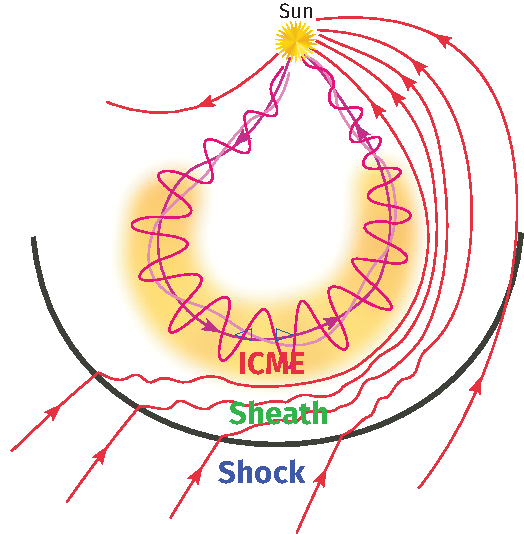
\includegraphics[width=\textwidth]{images/ZurbuchenRichardson-adapted.pdf}\\
            \scriptsize adapted from Zurbuchen and Richardson (2006)
        \end{column}
    \end{columns}
\end{frame}

\begin{frame}{Observation of (I)CMEs}
    \vskip3mm
    \begin{columns}[t]
        \begin{column}{0.45\textwidth}
            \textbf{Remote sensing:} CME
            
            \vskip-5mm\hskip-4mm
            \animategraphics[poster=19]{30}{plots/lightbulb_cme_anim/}{000}{048}
        \end{column}
        \begin{column}{0.45\textwidth}
            \textbf{In situ:} ICME

            %% Creator: Matplotlib, PGF backend
%%
%% To include the figure in your LaTeX document, write
%%   \input{<filename>.pgf}
%%
%% Make sure the required packages are loaded in your preamble
%%   \usepackage{pgf}
%%
%% and, on pdftex
%%   \usepackage[utf8]{inputenc}\DeclareUnicodeCharacter{2212}{-}
%%
%% or, on luatex and xetex
%%   \usepackage{unicode-math}
%%
%% Figures using additional raster images can only be included by \input if
%% they are in the same directory as the main LaTeX file. For loading figures
%% from other directories you can use the `import` package
%%   \usepackage{import}
%%
%% and then include the figures with
%%   \import{<path to file>}{<filename>.pgf}
%%
%% Matplotlib used the following preamble
%%   \usepackage{fontspec}
%%
\begingroup%
\makeatletter%
\begin{pgfpicture}%
\pgfpathrectangle{\pgfpointorigin}{\pgfqpoint{2.500000in}{2.500000in}}%
\pgfusepath{use as bounding box, clip}%
\begin{pgfscope}%
\pgfsetbuttcap%
\pgfsetmiterjoin%
\definecolor{currentfill}{rgb}{1.000000,1.000000,1.000000}%
\pgfsetfillcolor{currentfill}%
\pgfsetlinewidth{0.000000pt}%
\definecolor{currentstroke}{rgb}{1.000000,1.000000,1.000000}%
\pgfsetstrokecolor{currentstroke}%
\pgfsetdash{}{0pt}%
\pgfpathmoveto{\pgfqpoint{0.000000in}{0.000000in}}%
\pgfpathlineto{\pgfqpoint{2.500000in}{0.000000in}}%
\pgfpathlineto{\pgfqpoint{2.500000in}{2.500000in}}%
\pgfpathlineto{\pgfqpoint{0.000000in}{2.500000in}}%
\pgfpathclose%
\pgfusepath{fill}%
\end{pgfscope}%
\begin{pgfscope}%
\pgfsetbuttcap%
\pgfsetmiterjoin%
\definecolor{currentfill}{rgb}{1.000000,1.000000,1.000000}%
\pgfsetfillcolor{currentfill}%
\pgfsetlinewidth{0.000000pt}%
\definecolor{currentstroke}{rgb}{0.000000,0.000000,0.000000}%
\pgfsetstrokecolor{currentstroke}%
\pgfsetstrokeopacity{0.000000}%
\pgfsetdash{}{0pt}%
\pgfpathmoveto{\pgfqpoint{0.588735in}{1.707388in}}%
\pgfpathlineto{\pgfqpoint{1.879401in}{1.707388in}}%
\pgfpathlineto{\pgfqpoint{1.879401in}{2.347404in}}%
\pgfpathlineto{\pgfqpoint{0.588735in}{2.347404in}}%
\pgfpathclose%
\pgfusepath{fill}%
\end{pgfscope}%
\begin{pgfscope}%
\pgfsetbuttcap%
\pgfsetroundjoin%
\definecolor{currentfill}{rgb}{0.000000,0.000000,0.000000}%
\pgfsetfillcolor{currentfill}%
\pgfsetlinewidth{0.803000pt}%
\definecolor{currentstroke}{rgb}{0.000000,0.000000,0.000000}%
\pgfsetstrokecolor{currentstroke}%
\pgfsetdash{}{0pt}%
\pgfsys@defobject{currentmarker}{\pgfqpoint{0.000000in}{-0.048611in}}{\pgfqpoint{0.000000in}{0.000000in}}{%
\pgfpathmoveto{\pgfqpoint{0.000000in}{0.000000in}}%
\pgfpathlineto{\pgfqpoint{0.000000in}{-0.048611in}}%
\pgfusepath{stroke,fill}%
}%
\begin{pgfscope}%
\pgfsys@transformshift{1.134103in}{1.707388in}%
\pgfsys@useobject{currentmarker}{}%
\end{pgfscope}%
\end{pgfscope}%
\begin{pgfscope}%
\pgfsetbuttcap%
\pgfsetroundjoin%
\definecolor{currentfill}{rgb}{0.000000,0.000000,0.000000}%
\pgfsetfillcolor{currentfill}%
\pgfsetlinewidth{0.803000pt}%
\definecolor{currentstroke}{rgb}{0.000000,0.000000,0.000000}%
\pgfsetstrokecolor{currentstroke}%
\pgfsetdash{}{0pt}%
\pgfsys@defobject{currentmarker}{\pgfqpoint{0.000000in}{-0.048611in}}{\pgfqpoint{0.000000in}{0.000000in}}{%
\pgfpathmoveto{\pgfqpoint{0.000000in}{0.000000in}}%
\pgfpathlineto{\pgfqpoint{0.000000in}{-0.048611in}}%
\pgfusepath{stroke,fill}%
}%
\begin{pgfscope}%
\pgfsys@transformshift{1.821211in}{1.707388in}%
\pgfsys@useobject{currentmarker}{}%
\end{pgfscope}%
\end{pgfscope}%
\begin{pgfscope}%
\pgfsetbuttcap%
\pgfsetroundjoin%
\definecolor{currentfill}{rgb}{0.000000,0.000000,0.000000}%
\pgfsetfillcolor{currentfill}%
\pgfsetlinewidth{0.602250pt}%
\definecolor{currentstroke}{rgb}{0.000000,0.000000,0.000000}%
\pgfsetstrokecolor{currentstroke}%
\pgfsetdash{}{0pt}%
\pgfsys@defobject{currentmarker}{\pgfqpoint{0.000000in}{-0.027778in}}{\pgfqpoint{0.000000in}{0.000000in}}{%
\pgfpathmoveto{\pgfqpoint{0.000000in}{0.000000in}}%
\pgfpathlineto{\pgfqpoint{0.000000in}{-0.027778in}}%
\pgfusepath{stroke,fill}%
}%
\begin{pgfscope}%
\pgfsys@transformshift{0.618772in}{1.707388in}%
\pgfsys@useobject{currentmarker}{}%
\end{pgfscope}%
\end{pgfscope}%
\begin{pgfscope}%
\pgfsetbuttcap%
\pgfsetroundjoin%
\definecolor{currentfill}{rgb}{0.000000,0.000000,0.000000}%
\pgfsetfillcolor{currentfill}%
\pgfsetlinewidth{0.602250pt}%
\definecolor{currentstroke}{rgb}{0.000000,0.000000,0.000000}%
\pgfsetstrokecolor{currentstroke}%
\pgfsetdash{}{0pt}%
\pgfsys@defobject{currentmarker}{\pgfqpoint{0.000000in}{-0.027778in}}{\pgfqpoint{0.000000in}{0.000000in}}{%
\pgfpathmoveto{\pgfqpoint{0.000000in}{0.000000in}}%
\pgfpathlineto{\pgfqpoint{0.000000in}{-0.027778in}}%
\pgfusepath{stroke,fill}%
}%
\begin{pgfscope}%
\pgfsys@transformshift{0.790549in}{1.707388in}%
\pgfsys@useobject{currentmarker}{}%
\end{pgfscope}%
\end{pgfscope}%
\begin{pgfscope}%
\pgfsetbuttcap%
\pgfsetroundjoin%
\definecolor{currentfill}{rgb}{0.000000,0.000000,0.000000}%
\pgfsetfillcolor{currentfill}%
\pgfsetlinewidth{0.602250pt}%
\definecolor{currentstroke}{rgb}{0.000000,0.000000,0.000000}%
\pgfsetstrokecolor{currentstroke}%
\pgfsetdash{}{0pt}%
\pgfsys@defobject{currentmarker}{\pgfqpoint{0.000000in}{-0.027778in}}{\pgfqpoint{0.000000in}{0.000000in}}{%
\pgfpathmoveto{\pgfqpoint{0.000000in}{0.000000in}}%
\pgfpathlineto{\pgfqpoint{0.000000in}{-0.027778in}}%
\pgfusepath{stroke,fill}%
}%
\begin{pgfscope}%
\pgfsys@transformshift{0.962326in}{1.707388in}%
\pgfsys@useobject{currentmarker}{}%
\end{pgfscope}%
\end{pgfscope}%
\begin{pgfscope}%
\pgfsetbuttcap%
\pgfsetroundjoin%
\definecolor{currentfill}{rgb}{0.000000,0.000000,0.000000}%
\pgfsetfillcolor{currentfill}%
\pgfsetlinewidth{0.602250pt}%
\definecolor{currentstroke}{rgb}{0.000000,0.000000,0.000000}%
\pgfsetstrokecolor{currentstroke}%
\pgfsetdash{}{0pt}%
\pgfsys@defobject{currentmarker}{\pgfqpoint{0.000000in}{-0.027778in}}{\pgfqpoint{0.000000in}{0.000000in}}{%
\pgfpathmoveto{\pgfqpoint{0.000000in}{0.000000in}}%
\pgfpathlineto{\pgfqpoint{0.000000in}{-0.027778in}}%
\pgfusepath{stroke,fill}%
}%
\begin{pgfscope}%
\pgfsys@transformshift{1.305880in}{1.707388in}%
\pgfsys@useobject{currentmarker}{}%
\end{pgfscope}%
\end{pgfscope}%
\begin{pgfscope}%
\pgfsetbuttcap%
\pgfsetroundjoin%
\definecolor{currentfill}{rgb}{0.000000,0.000000,0.000000}%
\pgfsetfillcolor{currentfill}%
\pgfsetlinewidth{0.602250pt}%
\definecolor{currentstroke}{rgb}{0.000000,0.000000,0.000000}%
\pgfsetstrokecolor{currentstroke}%
\pgfsetdash{}{0pt}%
\pgfsys@defobject{currentmarker}{\pgfqpoint{0.000000in}{-0.027778in}}{\pgfqpoint{0.000000in}{0.000000in}}{%
\pgfpathmoveto{\pgfqpoint{0.000000in}{0.000000in}}%
\pgfpathlineto{\pgfqpoint{0.000000in}{-0.027778in}}%
\pgfusepath{stroke,fill}%
}%
\begin{pgfscope}%
\pgfsys@transformshift{1.477657in}{1.707388in}%
\pgfsys@useobject{currentmarker}{}%
\end{pgfscope}%
\end{pgfscope}%
\begin{pgfscope}%
\pgfsetbuttcap%
\pgfsetroundjoin%
\definecolor{currentfill}{rgb}{0.000000,0.000000,0.000000}%
\pgfsetfillcolor{currentfill}%
\pgfsetlinewidth{0.602250pt}%
\definecolor{currentstroke}{rgb}{0.000000,0.000000,0.000000}%
\pgfsetstrokecolor{currentstroke}%
\pgfsetdash{}{0pt}%
\pgfsys@defobject{currentmarker}{\pgfqpoint{0.000000in}{-0.027778in}}{\pgfqpoint{0.000000in}{0.000000in}}{%
\pgfpathmoveto{\pgfqpoint{0.000000in}{0.000000in}}%
\pgfpathlineto{\pgfqpoint{0.000000in}{-0.027778in}}%
\pgfusepath{stroke,fill}%
}%
\begin{pgfscope}%
\pgfsys@transformshift{1.649434in}{1.707388in}%
\pgfsys@useobject{currentmarker}{}%
\end{pgfscope}%
\end{pgfscope}%
\begin{pgfscope}%
\pgfsetbuttcap%
\pgfsetroundjoin%
\definecolor{currentfill}{rgb}{0.000000,0.000000,0.000000}%
\pgfsetfillcolor{currentfill}%
\pgfsetlinewidth{0.803000pt}%
\definecolor{currentstroke}{rgb}{0.000000,0.000000,0.000000}%
\pgfsetstrokecolor{currentstroke}%
\pgfsetdash{}{0pt}%
\pgfsys@defobject{currentmarker}{\pgfqpoint{-0.048611in}{0.000000in}}{\pgfqpoint{-0.000000in}{0.000000in}}{%
\pgfpathmoveto{\pgfqpoint{-0.000000in}{0.000000in}}%
\pgfpathlineto{\pgfqpoint{-0.048611in}{0.000000in}}%
\pgfusepath{stroke,fill}%
}%
\begin{pgfscope}%
\pgfsys@transformshift{0.588735in}{1.965968in}%
\pgfsys@useobject{currentmarker}{}%
\end{pgfscope}%
\end{pgfscope}%
\begin{pgfscope}%
\definecolor{textcolor}{rgb}{0.000000,0.000000,0.000000}%
\pgfsetstrokecolor{textcolor}%
\pgfsetfillcolor{textcolor}%
\pgftext[x=0.432484in, y=1.927412in, left, base]{\color{textcolor}\rmfamily\fontsize{8.000000}{9.600000}\selectfont \(\displaystyle {0}\)}%
\end{pgfscope}%
\begin{pgfscope}%
\pgfsetbuttcap%
\pgfsetroundjoin%
\definecolor{currentfill}{rgb}{0.000000,0.000000,0.000000}%
\pgfsetfillcolor{currentfill}%
\pgfsetlinewidth{0.803000pt}%
\definecolor{currentstroke}{rgb}{0.000000,0.000000,0.000000}%
\pgfsetstrokecolor{currentstroke}%
\pgfsetdash{}{0pt}%
\pgfsys@defobject{currentmarker}{\pgfqpoint{-0.048611in}{0.000000in}}{\pgfqpoint{-0.000000in}{0.000000in}}{%
\pgfpathmoveto{\pgfqpoint{-0.000000in}{0.000000in}}%
\pgfpathlineto{\pgfqpoint{-0.048611in}{0.000000in}}%
\pgfusepath{stroke,fill}%
}%
\begin{pgfscope}%
\pgfsys@transformshift{0.588735in}{2.320728in}%
\pgfsys@useobject{currentmarker}{}%
\end{pgfscope}%
\end{pgfscope}%
\begin{pgfscope}%
\definecolor{textcolor}{rgb}{0.000000,0.000000,0.000000}%
\pgfsetstrokecolor{textcolor}%
\pgfsetfillcolor{textcolor}%
\pgftext[x=0.373456in, y=2.282173in, left, base]{\color{textcolor}\rmfamily\fontsize{8.000000}{9.600000}\selectfont \(\displaystyle {25}\)}%
\end{pgfscope}%
\begin{pgfscope}%
\definecolor{textcolor}{rgb}{0.000000,0.000000,0.000000}%
\pgfsetstrokecolor{textcolor}%
\pgfsetfillcolor{textcolor}%
\pgftext[x=0.317900in,y=2.027396in,,bottom,rotate=90.000000]{\color{textcolor}\rmfamily\fontsize{9.000000}{10.800000}\selectfont B [nT]}%
\end{pgfscope}%
\begin{pgfscope}%
\pgfpathrectangle{\pgfqpoint{0.588735in}{1.707388in}}{\pgfqpoint{1.290666in}{0.640015in}}%
\pgfusepath{clip}%
\pgfsetrectcap%
\pgfsetroundjoin%
\pgfsetlinewidth{1.003750pt}%
\definecolor{currentstroke}{rgb}{0.121569,0.466667,0.705882}%
\pgfsetstrokecolor{currentstroke}%
\pgfsetdash{}{0pt}%
\pgfpathmoveto{\pgfqpoint{0.647402in}{2.056776in}}%
\pgfpathlineto{\pgfqpoint{0.647879in}{2.055835in}}%
\pgfpathlineto{\pgfqpoint{0.648356in}{2.057670in}}%
\pgfpathlineto{\pgfqpoint{0.648833in}{2.056871in}}%
\pgfpathlineto{\pgfqpoint{0.650742in}{2.056733in}}%
\pgfpathlineto{\pgfqpoint{0.651219in}{2.058613in}}%
\pgfpathlineto{\pgfqpoint{0.651696in}{2.056857in}}%
\pgfpathlineto{\pgfqpoint{0.652173in}{2.054952in}}%
\pgfpathlineto{\pgfqpoint{0.652650in}{2.058010in}}%
\pgfpathlineto{\pgfqpoint{0.653605in}{2.057794in}}%
\pgfpathlineto{\pgfqpoint{0.658853in}{2.061994in}}%
\pgfpathlineto{\pgfqpoint{0.662194in}{2.062093in}}%
\pgfpathlineto{\pgfqpoint{0.663625in}{2.063676in}}%
\pgfpathlineto{\pgfqpoint{0.667920in}{2.061033in}}%
\pgfpathlineto{\pgfqpoint{0.669351in}{2.062218in}}%
\pgfpathlineto{\pgfqpoint{0.670305in}{2.061607in}}%
\pgfpathlineto{\pgfqpoint{0.670782in}{2.059965in}}%
\pgfpathlineto{\pgfqpoint{0.671737in}{2.060454in}}%
\pgfpathlineto{\pgfqpoint{0.679371in}{2.062874in}}%
\pgfpathlineto{\pgfqpoint{0.682711in}{2.061969in}}%
\pgfpathlineto{\pgfqpoint{0.684620in}{2.062239in}}%
\pgfpathlineto{\pgfqpoint{0.685574in}{2.062746in}}%
\pgfpathlineto{\pgfqpoint{0.686052in}{2.061942in}}%
\pgfpathlineto{\pgfqpoint{0.691777in}{2.061852in}}%
\pgfpathlineto{\pgfqpoint{0.693209in}{2.062973in}}%
\pgfpathlineto{\pgfqpoint{0.693686in}{2.062396in}}%
\pgfpathlineto{\pgfqpoint{0.697980in}{2.062115in}}%
\pgfpathlineto{\pgfqpoint{0.698935in}{2.062828in}}%
\pgfpathlineto{\pgfqpoint{0.699412in}{2.062022in}}%
\pgfpathlineto{\pgfqpoint{0.702275in}{2.062320in}}%
\pgfpathlineto{\pgfqpoint{0.703706in}{2.062235in}}%
\pgfpathlineto{\pgfqpoint{0.704184in}{2.062895in}}%
\pgfpathlineto{\pgfqpoint{0.704661in}{2.062093in}}%
\pgfpathlineto{\pgfqpoint{0.705615in}{2.062842in}}%
\pgfpathlineto{\pgfqpoint{0.707047in}{2.063721in}}%
\pgfpathlineto{\pgfqpoint{0.707524in}{2.063158in}}%
\pgfpathlineto{\pgfqpoint{0.710387in}{2.061437in}}%
\pgfpathlineto{\pgfqpoint{0.713250in}{2.062097in}}%
\pgfpathlineto{\pgfqpoint{0.715158in}{2.061377in}}%
\pgfpathlineto{\pgfqpoint{0.716590in}{2.061805in}}%
\pgfpathlineto{\pgfqpoint{0.717544in}{2.061639in}}%
\pgfpathlineto{\pgfqpoint{0.718021in}{2.063080in}}%
\pgfpathlineto{\pgfqpoint{0.718498in}{2.061573in}}%
\pgfpathlineto{\pgfqpoint{0.720407in}{2.063106in}}%
\pgfpathlineto{\pgfqpoint{0.722793in}{2.062441in}}%
\pgfpathlineto{\pgfqpoint{0.727564in}{2.063225in}}%
\pgfpathlineto{\pgfqpoint{0.729950in}{2.063276in}}%
\pgfpathlineto{\pgfqpoint{0.731382in}{2.063211in}}%
\pgfpathlineto{\pgfqpoint{0.737107in}{2.062909in}}%
\pgfpathlineto{\pgfqpoint{0.737585in}{2.063593in}}%
\pgfpathlineto{\pgfqpoint{0.738062in}{2.063168in}}%
\pgfpathlineto{\pgfqpoint{0.740925in}{2.060901in}}%
\pgfpathlineto{\pgfqpoint{0.741402in}{2.061597in}}%
\pgfpathlineto{\pgfqpoint{0.741879in}{2.061107in}}%
\pgfpathlineto{\pgfqpoint{0.742833in}{2.059848in}}%
\pgfpathlineto{\pgfqpoint{0.744265in}{2.061536in}}%
\pgfpathlineto{\pgfqpoint{0.744742in}{2.060948in}}%
\pgfpathlineto{\pgfqpoint{0.745219in}{2.061469in}}%
\pgfpathlineto{\pgfqpoint{0.749514in}{2.062945in}}%
\pgfpathlineto{\pgfqpoint{0.751422in}{2.129824in}}%
\pgfpathlineto{\pgfqpoint{0.752377in}{2.112576in}}%
\pgfpathlineto{\pgfqpoint{0.752854in}{2.117261in}}%
\pgfpathlineto{\pgfqpoint{0.753331in}{2.114183in}}%
\pgfpathlineto{\pgfqpoint{0.753808in}{2.118504in}}%
\pgfpathlineto{\pgfqpoint{0.754762in}{2.117937in}}%
\pgfpathlineto{\pgfqpoint{0.755717in}{2.120955in}}%
\pgfpathlineto{\pgfqpoint{0.757148in}{2.135380in}}%
\pgfpathlineto{\pgfqpoint{0.759057in}{2.120480in}}%
\pgfpathlineto{\pgfqpoint{0.760011in}{2.131524in}}%
\pgfpathlineto{\pgfqpoint{0.760488in}{2.126859in}}%
\pgfpathlineto{\pgfqpoint{0.760965in}{2.125088in}}%
\pgfpathlineto{\pgfqpoint{0.761443in}{2.127721in}}%
\pgfpathlineto{\pgfqpoint{0.762874in}{2.120210in}}%
\pgfpathlineto{\pgfqpoint{0.763828in}{2.128600in}}%
\pgfpathlineto{\pgfqpoint{0.764306in}{2.127081in}}%
\pgfpathlineto{\pgfqpoint{0.764783in}{2.130424in}}%
\pgfpathlineto{\pgfqpoint{0.765260in}{2.126596in}}%
\pgfpathlineto{\pgfqpoint{0.766214in}{2.121717in}}%
\pgfpathlineto{\pgfqpoint{0.766691in}{2.122098in}}%
\pgfpathlineto{\pgfqpoint{0.769077in}{2.115403in}}%
\pgfpathlineto{\pgfqpoint{0.769554in}{2.118071in}}%
\pgfpathlineto{\pgfqpoint{0.770031in}{2.113988in}}%
\pgfpathlineto{\pgfqpoint{0.770509in}{2.115091in}}%
\pgfpathlineto{\pgfqpoint{0.771463in}{2.130474in}}%
\pgfpathlineto{\pgfqpoint{0.772417in}{2.129555in}}%
\pgfpathlineto{\pgfqpoint{0.773372in}{2.132421in}}%
\pgfpathlineto{\pgfqpoint{0.775757in}{2.144677in}}%
\pgfpathlineto{\pgfqpoint{0.778143in}{2.132730in}}%
\pgfpathlineto{\pgfqpoint{0.779097in}{2.135171in}}%
\pgfpathlineto{\pgfqpoint{0.780529in}{2.135678in}}%
\pgfpathlineto{\pgfqpoint{0.782438in}{2.138509in}}%
\pgfpathlineto{\pgfqpoint{0.782915in}{2.137200in}}%
\pgfpathlineto{\pgfqpoint{0.783392in}{2.138471in}}%
\pgfpathlineto{\pgfqpoint{0.785778in}{2.147406in}}%
\pgfpathlineto{\pgfqpoint{0.786255in}{2.144636in}}%
\pgfpathlineto{\pgfqpoint{0.787686in}{2.129810in}}%
\pgfpathlineto{\pgfqpoint{0.788163in}{2.121959in}}%
\pgfpathlineto{\pgfqpoint{0.788641in}{2.138566in}}%
\pgfpathlineto{\pgfqpoint{0.789595in}{2.137817in}}%
\pgfpathlineto{\pgfqpoint{0.790549in}{2.145161in}}%
\pgfpathlineto{\pgfqpoint{0.791026in}{2.141569in}}%
\pgfpathlineto{\pgfqpoint{0.792458in}{2.126592in}}%
\pgfpathlineto{\pgfqpoint{0.792935in}{2.152368in}}%
\pgfpathlineto{\pgfqpoint{0.793889in}{2.149379in}}%
\pgfpathlineto{\pgfqpoint{0.795321in}{2.153629in}}%
\pgfpathlineto{\pgfqpoint{0.796752in}{2.150765in}}%
\pgfpathlineto{\pgfqpoint{0.798661in}{2.147581in}}%
\pgfpathlineto{\pgfqpoint{0.801524in}{2.158205in}}%
\pgfpathlineto{\pgfqpoint{0.802478in}{2.102569in}}%
\pgfpathlineto{\pgfqpoint{0.803433in}{2.049840in}}%
\pgfpathlineto{\pgfqpoint{0.803910in}{2.081169in}}%
\pgfpathlineto{\pgfqpoint{0.804387in}{2.119271in}}%
\pgfpathlineto{\pgfqpoint{0.805341in}{2.115921in}}%
\pgfpathlineto{\pgfqpoint{0.805818in}{2.115396in}}%
\pgfpathlineto{\pgfqpoint{0.807727in}{2.139030in}}%
\pgfpathlineto{\pgfqpoint{0.808204in}{2.156081in}}%
\pgfpathlineto{\pgfqpoint{0.808681in}{2.139002in}}%
\pgfpathlineto{\pgfqpoint{0.810113in}{2.035940in}}%
\pgfpathlineto{\pgfqpoint{0.810590in}{2.048712in}}%
\pgfpathlineto{\pgfqpoint{0.811067in}{2.070852in}}%
\pgfpathlineto{\pgfqpoint{0.811544in}{2.064754in}}%
\pgfpathlineto{\pgfqpoint{0.812499in}{2.025677in}}%
\pgfpathlineto{\pgfqpoint{0.812976in}{2.049084in}}%
\pgfpathlineto{\pgfqpoint{0.813453in}{2.048017in}}%
\pgfpathlineto{\pgfqpoint{0.814407in}{2.021984in}}%
\pgfpathlineto{\pgfqpoint{0.814884in}{2.035054in}}%
\pgfpathlineto{\pgfqpoint{0.816793in}{2.052522in}}%
\pgfpathlineto{\pgfqpoint{0.817747in}{2.001988in}}%
\pgfpathlineto{\pgfqpoint{0.818224in}{2.006779in}}%
\pgfpathlineto{\pgfqpoint{0.820610in}{1.975482in}}%
\pgfpathlineto{\pgfqpoint{0.821087in}{1.982393in}}%
\pgfpathlineto{\pgfqpoint{0.822042in}{1.990907in}}%
\pgfpathlineto{\pgfqpoint{0.822519in}{1.986955in}}%
\pgfpathlineto{\pgfqpoint{0.822996in}{1.990127in}}%
\pgfpathlineto{\pgfqpoint{0.823473in}{1.978072in}}%
\pgfpathlineto{\pgfqpoint{0.823950in}{1.988878in}}%
\pgfpathlineto{\pgfqpoint{0.825382in}{2.015700in}}%
\pgfpathlineto{\pgfqpoint{0.826336in}{1.993866in}}%
\pgfpathlineto{\pgfqpoint{0.829676in}{2.076273in}}%
\pgfpathlineto{\pgfqpoint{0.830153in}{2.075957in}}%
\pgfpathlineto{\pgfqpoint{0.831108in}{2.050069in}}%
\pgfpathlineto{\pgfqpoint{0.832062in}{2.054810in}}%
\pgfpathlineto{\pgfqpoint{0.833493in}{2.093596in}}%
\pgfpathlineto{\pgfqpoint{0.833971in}{2.092599in}}%
\pgfpathlineto{\pgfqpoint{0.834448in}{2.092408in}}%
\pgfpathlineto{\pgfqpoint{0.834925in}{2.093696in}}%
\pgfpathlineto{\pgfqpoint{0.835402in}{2.093405in}}%
\pgfpathlineto{\pgfqpoint{0.835879in}{2.092564in}}%
\pgfpathlineto{\pgfqpoint{0.836356in}{2.093139in}}%
\pgfpathlineto{\pgfqpoint{0.838265in}{2.100794in}}%
\pgfpathlineto{\pgfqpoint{0.838742in}{2.096931in}}%
\pgfpathlineto{\pgfqpoint{0.839697in}{2.107386in}}%
\pgfpathlineto{\pgfqpoint{0.840174in}{2.102373in}}%
\pgfpathlineto{\pgfqpoint{0.841128in}{2.094746in}}%
\pgfpathlineto{\pgfqpoint{0.841605in}{2.086515in}}%
\pgfpathlineto{\pgfqpoint{0.843037in}{2.011409in}}%
\pgfpathlineto{\pgfqpoint{0.843514in}{2.100833in}}%
\pgfpathlineto{\pgfqpoint{0.844468in}{2.077987in}}%
\pgfpathlineto{\pgfqpoint{0.844945in}{2.074471in}}%
\pgfpathlineto{\pgfqpoint{0.845422in}{2.076745in}}%
\pgfpathlineto{\pgfqpoint{0.845900in}{2.088012in}}%
\pgfpathlineto{\pgfqpoint{0.846377in}{2.077168in}}%
\pgfpathlineto{\pgfqpoint{0.847331in}{2.047850in}}%
\pgfpathlineto{\pgfqpoint{0.847808in}{2.061022in}}%
\pgfpathlineto{\pgfqpoint{0.848285in}{2.070825in}}%
\pgfpathlineto{\pgfqpoint{0.848763in}{2.058929in}}%
\pgfpathlineto{\pgfqpoint{0.849240in}{2.068915in}}%
\pgfpathlineto{\pgfqpoint{0.850194in}{2.041730in}}%
\pgfpathlineto{\pgfqpoint{0.850671in}{2.051866in}}%
\pgfpathlineto{\pgfqpoint{0.851148in}{2.061281in}}%
\pgfpathlineto{\pgfqpoint{0.851626in}{2.046523in}}%
\pgfpathlineto{\pgfqpoint{0.852103in}{2.048892in}}%
\pgfpathlineto{\pgfqpoint{0.852580in}{2.052068in}}%
\pgfpathlineto{\pgfqpoint{0.854966in}{2.029789in}}%
\pgfpathlineto{\pgfqpoint{0.857351in}{2.067926in}}%
\pgfpathlineto{\pgfqpoint{0.857829in}{2.068375in}}%
\pgfpathlineto{\pgfqpoint{0.861169in}{2.011913in}}%
\pgfpathlineto{\pgfqpoint{0.862600in}{2.027579in}}%
\pgfpathlineto{\pgfqpoint{0.863077in}{2.024844in}}%
\pgfpathlineto{\pgfqpoint{0.863554in}{2.031177in}}%
\pgfpathlineto{\pgfqpoint{0.864032in}{2.023950in}}%
\pgfpathlineto{\pgfqpoint{0.864509in}{2.030995in}}%
\pgfpathlineto{\pgfqpoint{0.865463in}{2.033249in}}%
\pgfpathlineto{\pgfqpoint{0.865940in}{2.001135in}}%
\pgfpathlineto{\pgfqpoint{0.866895in}{2.002707in}}%
\pgfpathlineto{\pgfqpoint{0.867372in}{1.984145in}}%
\pgfpathlineto{\pgfqpoint{0.867849in}{1.998233in}}%
\pgfpathlineto{\pgfqpoint{0.869280in}{2.020520in}}%
\pgfpathlineto{\pgfqpoint{0.870712in}{2.022658in}}%
\pgfpathlineto{\pgfqpoint{0.871666in}{1.996637in}}%
\pgfpathlineto{\pgfqpoint{0.874052in}{2.062775in}}%
\pgfpathlineto{\pgfqpoint{0.875006in}{2.032998in}}%
\pgfpathlineto{\pgfqpoint{0.875961in}{2.034500in}}%
\pgfpathlineto{\pgfqpoint{0.876438in}{2.034177in}}%
\pgfpathlineto{\pgfqpoint{0.876915in}{2.035278in}}%
\pgfpathlineto{\pgfqpoint{0.878346in}{2.032357in}}%
\pgfpathlineto{\pgfqpoint{0.878824in}{2.031792in}}%
\pgfpathlineto{\pgfqpoint{0.879301in}{2.036629in}}%
\pgfpathlineto{\pgfqpoint{0.879778in}{2.026585in}}%
\pgfpathlineto{\pgfqpoint{0.880255in}{2.030406in}}%
\pgfpathlineto{\pgfqpoint{0.880732in}{2.033074in}}%
\pgfpathlineto{\pgfqpoint{0.883595in}{2.012331in}}%
\pgfpathlineto{\pgfqpoint{0.885027in}{2.016773in}}%
\pgfpathlineto{\pgfqpoint{0.885981in}{1.999050in}}%
\pgfpathlineto{\pgfqpoint{0.887412in}{2.053083in}}%
\pgfpathlineto{\pgfqpoint{0.887890in}{2.053735in}}%
\pgfpathlineto{\pgfqpoint{0.889798in}{2.046356in}}%
\pgfpathlineto{\pgfqpoint{0.890753in}{2.049411in}}%
\pgfpathlineto{\pgfqpoint{0.891230in}{2.048311in}}%
\pgfpathlineto{\pgfqpoint{0.891707in}{2.047577in}}%
\pgfpathlineto{\pgfqpoint{0.892661in}{2.054487in}}%
\pgfpathlineto{\pgfqpoint{0.893138in}{2.052848in}}%
\pgfpathlineto{\pgfqpoint{0.893615in}{2.053746in}}%
\pgfpathlineto{\pgfqpoint{0.895047in}{2.049698in}}%
\pgfpathlineto{\pgfqpoint{0.896001in}{2.055835in}}%
\pgfpathlineto{\pgfqpoint{0.896478in}{2.055300in}}%
\pgfpathlineto{\pgfqpoint{0.897433in}{2.053015in}}%
\pgfpathlineto{\pgfqpoint{0.899341in}{2.062597in}}%
\pgfpathlineto{\pgfqpoint{0.899819in}{2.062992in}}%
\pgfpathlineto{\pgfqpoint{0.902204in}{2.059025in}}%
\pgfpathlineto{\pgfqpoint{0.903159in}{2.060330in}}%
\pgfpathlineto{\pgfqpoint{0.906022in}{2.055953in}}%
\pgfpathlineto{\pgfqpoint{0.906976in}{2.057070in}}%
\pgfpathlineto{\pgfqpoint{0.907453in}{2.055523in}}%
\pgfpathlineto{\pgfqpoint{0.907930in}{2.054810in}}%
\pgfpathlineto{\pgfqpoint{0.908407in}{2.055506in}}%
\pgfpathlineto{\pgfqpoint{0.912702in}{2.057482in}}%
\pgfpathlineto{\pgfqpoint{0.913179in}{2.058234in}}%
\pgfpathlineto{\pgfqpoint{0.913656in}{2.054374in}}%
\pgfpathlineto{\pgfqpoint{0.914133in}{2.056566in}}%
\pgfpathlineto{\pgfqpoint{0.915088in}{2.054998in}}%
\pgfpathlineto{\pgfqpoint{0.916042in}{2.051192in}}%
\pgfpathlineto{\pgfqpoint{0.916519in}{2.054796in}}%
\pgfpathlineto{\pgfqpoint{0.917951in}{2.045828in}}%
\pgfpathlineto{\pgfqpoint{0.918428in}{2.046903in}}%
\pgfpathlineto{\pgfqpoint{0.919859in}{2.041989in}}%
\pgfpathlineto{\pgfqpoint{0.920336in}{2.052596in}}%
\pgfpathlineto{\pgfqpoint{0.921291in}{2.049326in}}%
\pgfpathlineto{\pgfqpoint{0.921768in}{2.048194in}}%
\pgfpathlineto{\pgfqpoint{0.922245in}{2.049201in}}%
\pgfpathlineto{\pgfqpoint{0.923676in}{2.055154in}}%
\pgfpathlineto{\pgfqpoint{0.924154in}{2.055247in}}%
\pgfpathlineto{\pgfqpoint{0.925108in}{2.053182in}}%
\pgfpathlineto{\pgfqpoint{0.925585in}{2.054434in}}%
\pgfpathlineto{\pgfqpoint{0.927494in}{2.060756in}}%
\pgfpathlineto{\pgfqpoint{0.927971in}{2.058642in}}%
\pgfpathlineto{\pgfqpoint{0.928448in}{2.042653in}}%
\pgfpathlineto{\pgfqpoint{0.928925in}{2.054477in}}%
\pgfpathlineto{\pgfqpoint{0.932742in}{2.057471in}}%
\pgfpathlineto{\pgfqpoint{0.934174in}{2.062358in}}%
\pgfpathlineto{\pgfqpoint{0.936560in}{2.057811in}}%
\pgfpathlineto{\pgfqpoint{0.937037in}{2.050546in}}%
\pgfpathlineto{\pgfqpoint{0.937991in}{2.052539in}}%
\pgfpathlineto{\pgfqpoint{0.938468in}{2.051837in}}%
\pgfpathlineto{\pgfqpoint{0.939900in}{2.039086in}}%
\pgfpathlineto{\pgfqpoint{0.940854in}{2.049365in}}%
\pgfpathlineto{\pgfqpoint{0.941331in}{2.049226in}}%
\pgfpathlineto{\pgfqpoint{0.943717in}{2.037856in}}%
\pgfpathlineto{\pgfqpoint{0.944194in}{2.041567in}}%
\pgfpathlineto{\pgfqpoint{0.944671in}{2.043291in}}%
\pgfpathlineto{\pgfqpoint{0.946580in}{2.059447in}}%
\pgfpathlineto{\pgfqpoint{0.947057in}{2.060660in}}%
\pgfpathlineto{\pgfqpoint{0.947534in}{2.059393in}}%
\pgfpathlineto{\pgfqpoint{0.948489in}{2.052753in}}%
\pgfpathlineto{\pgfqpoint{0.948966in}{2.055984in}}%
\pgfpathlineto{\pgfqpoint{0.949920in}{2.060557in}}%
\pgfpathlineto{\pgfqpoint{0.950874in}{2.049702in}}%
\pgfpathlineto{\pgfqpoint{0.951352in}{2.056606in}}%
\pgfpathlineto{\pgfqpoint{0.951829in}{2.053909in}}%
\pgfpathlineto{\pgfqpoint{0.952306in}{2.048162in}}%
\pgfpathlineto{\pgfqpoint{0.953260in}{2.071568in}}%
\pgfpathlineto{\pgfqpoint{0.954692in}{2.044483in}}%
\pgfpathlineto{\pgfqpoint{0.956123in}{2.053274in}}%
\pgfpathlineto{\pgfqpoint{0.956600in}{2.046402in}}%
\pgfpathlineto{\pgfqpoint{0.957078in}{2.056323in}}%
\pgfpathlineto{\pgfqpoint{0.957555in}{2.046491in}}%
\pgfpathlineto{\pgfqpoint{0.959463in}{2.016251in}}%
\pgfpathlineto{\pgfqpoint{0.961372in}{2.058223in}}%
\pgfpathlineto{\pgfqpoint{0.964712in}{2.081676in}}%
\pgfpathlineto{\pgfqpoint{0.966144in}{2.085164in}}%
\pgfpathlineto{\pgfqpoint{0.966621in}{2.082154in}}%
\pgfpathlineto{\pgfqpoint{0.967575in}{2.083056in}}%
\pgfpathlineto{\pgfqpoint{0.968529in}{2.083833in}}%
\pgfpathlineto{\pgfqpoint{0.969006in}{2.083425in}}%
\pgfpathlineto{\pgfqpoint{0.969484in}{2.081761in}}%
\pgfpathlineto{\pgfqpoint{0.969961in}{2.084007in}}%
\pgfpathlineto{\pgfqpoint{0.971392in}{2.083883in}}%
\pgfpathlineto{\pgfqpoint{0.972347in}{2.084817in}}%
\pgfpathlineto{\pgfqpoint{0.972824in}{2.080027in}}%
\pgfpathlineto{\pgfqpoint{0.973301in}{2.084511in}}%
\pgfpathlineto{\pgfqpoint{0.974255in}{2.085276in}}%
\pgfpathlineto{\pgfqpoint{0.974732in}{2.084663in}}%
\pgfpathlineto{\pgfqpoint{0.977595in}{2.098084in}}%
\pgfpathlineto{\pgfqpoint{0.978073in}{2.097442in}}%
\pgfpathlineto{\pgfqpoint{0.978550in}{2.098126in}}%
\pgfpathlineto{\pgfqpoint{0.979981in}{2.099462in}}%
\pgfpathlineto{\pgfqpoint{0.980458in}{2.096427in}}%
\pgfpathlineto{\pgfqpoint{0.980935in}{2.098080in}}%
\pgfpathlineto{\pgfqpoint{0.982367in}{2.103668in}}%
\pgfpathlineto{\pgfqpoint{0.982844in}{2.109429in}}%
\pgfpathlineto{\pgfqpoint{0.983321in}{2.107957in}}%
\pgfpathlineto{\pgfqpoint{0.984753in}{2.102898in}}%
\pgfpathlineto{\pgfqpoint{0.985707in}{2.105242in}}%
\pgfpathlineto{\pgfqpoint{0.988093in}{2.107130in}}%
\pgfpathlineto{\pgfqpoint{0.988570in}{2.106197in}}%
\pgfpathlineto{\pgfqpoint{0.990001in}{2.112164in}}%
\pgfpathlineto{\pgfqpoint{0.991910in}{2.106573in}}%
\pgfpathlineto{\pgfqpoint{0.992387in}{2.107457in}}%
\pgfpathlineto{\pgfqpoint{0.993819in}{2.121835in}}%
\pgfpathlineto{\pgfqpoint{0.994296in}{2.121001in}}%
\pgfpathlineto{\pgfqpoint{0.994773in}{2.124308in}}%
\pgfpathlineto{\pgfqpoint{0.995250in}{2.121949in}}%
\pgfpathlineto{\pgfqpoint{0.995727in}{2.119238in}}%
\pgfpathlineto{\pgfqpoint{0.996205in}{2.121168in}}%
\pgfpathlineto{\pgfqpoint{0.999545in}{2.124773in}}%
\pgfpathlineto{\pgfqpoint{1.000022in}{2.123332in}}%
\pgfpathlineto{\pgfqpoint{1.000499in}{2.124425in}}%
\pgfpathlineto{\pgfqpoint{1.001930in}{2.126465in}}%
\pgfpathlineto{\pgfqpoint{1.003839in}{2.128746in}}%
\pgfpathlineto{\pgfqpoint{1.004793in}{2.125586in}}%
\pgfpathlineto{\pgfqpoint{1.005271in}{2.127391in}}%
\pgfpathlineto{\pgfqpoint{1.007179in}{2.131275in}}%
\pgfpathlineto{\pgfqpoint{1.007656in}{2.129672in}}%
\pgfpathlineto{\pgfqpoint{1.008133in}{2.130442in}}%
\pgfpathlineto{\pgfqpoint{1.010996in}{2.131751in}}%
\pgfpathlineto{\pgfqpoint{1.012428in}{2.135666in}}%
\pgfpathlineto{\pgfqpoint{1.012905in}{2.135351in}}%
\pgfpathlineto{\pgfqpoint{1.014337in}{2.136111in}}%
\pgfpathlineto{\pgfqpoint{1.014814in}{2.134908in}}%
\pgfpathlineto{\pgfqpoint{1.015291in}{2.135969in}}%
\pgfpathlineto{\pgfqpoint{1.016722in}{2.137643in}}%
\pgfpathlineto{\pgfqpoint{1.017677in}{2.138417in}}%
\pgfpathlineto{\pgfqpoint{1.018631in}{2.136841in}}%
\pgfpathlineto{\pgfqpoint{1.019108in}{2.137257in}}%
\pgfpathlineto{\pgfqpoint{1.020062in}{2.138490in}}%
\pgfpathlineto{\pgfqpoint{1.021494in}{2.129345in}}%
\pgfpathlineto{\pgfqpoint{1.023403in}{2.138722in}}%
\pgfpathlineto{\pgfqpoint{1.025311in}{2.140049in}}%
\pgfpathlineto{\pgfqpoint{1.025788in}{2.139791in}}%
\pgfpathlineto{\pgfqpoint{1.026266in}{2.140896in}}%
\pgfpathlineto{\pgfqpoint{1.027220in}{2.137501in}}%
\pgfpathlineto{\pgfqpoint{1.028651in}{2.141088in}}%
\pgfpathlineto{\pgfqpoint{1.030560in}{2.138370in}}%
\pgfpathlineto{\pgfqpoint{1.032946in}{2.142237in}}%
\pgfpathlineto{\pgfqpoint{1.033423in}{2.142425in}}%
\pgfpathlineto{\pgfqpoint{1.034854in}{2.138963in}}%
\pgfpathlineto{\pgfqpoint{1.036286in}{2.139477in}}%
\pgfpathlineto{\pgfqpoint{1.037717in}{2.141162in}}%
\pgfpathlineto{\pgfqpoint{1.039149in}{2.143154in}}%
\pgfpathlineto{\pgfqpoint{1.039626in}{2.143564in}}%
\pgfpathlineto{\pgfqpoint{1.040580in}{2.131772in}}%
\pgfpathlineto{\pgfqpoint{1.042012in}{2.124794in}}%
\pgfpathlineto{\pgfqpoint{1.042489in}{2.122087in}}%
\pgfpathlineto{\pgfqpoint{1.042966in}{2.123543in}}%
\pgfpathlineto{\pgfqpoint{1.043443in}{2.124609in}}%
\pgfpathlineto{\pgfqpoint{1.045352in}{2.116829in}}%
\pgfpathlineto{\pgfqpoint{1.045829in}{2.118014in}}%
\pgfpathlineto{\pgfqpoint{1.047260in}{2.142450in}}%
\pgfpathlineto{\pgfqpoint{1.047738in}{2.138629in}}%
\pgfpathlineto{\pgfqpoint{1.048692in}{2.132383in}}%
\pgfpathlineto{\pgfqpoint{1.050601in}{2.143986in}}%
\pgfpathlineto{\pgfqpoint{1.051555in}{2.144242in}}%
\pgfpathlineto{\pgfqpoint{1.052986in}{2.134858in}}%
\pgfpathlineto{\pgfqpoint{1.053464in}{2.140886in}}%
\pgfpathlineto{\pgfqpoint{1.053941in}{2.140974in}}%
\pgfpathlineto{\pgfqpoint{1.054418in}{2.139904in}}%
\pgfpathlineto{\pgfqpoint{1.054895in}{2.140173in}}%
\pgfpathlineto{\pgfqpoint{1.055849in}{2.140453in}}%
\pgfpathlineto{\pgfqpoint{1.056326in}{2.138944in}}%
\pgfpathlineto{\pgfqpoint{1.057758in}{2.141638in}}%
\pgfpathlineto{\pgfqpoint{1.058712in}{2.139846in}}%
\pgfpathlineto{\pgfqpoint{1.060144in}{2.133258in}}%
\pgfpathlineto{\pgfqpoint{1.060621in}{2.133450in}}%
\pgfpathlineto{\pgfqpoint{1.062052in}{2.137265in}}%
\pgfpathlineto{\pgfqpoint{1.062530in}{2.136050in}}%
\pgfpathlineto{\pgfqpoint{1.063961in}{2.130491in}}%
\pgfpathlineto{\pgfqpoint{1.064438in}{2.130665in}}%
\pgfpathlineto{\pgfqpoint{1.067301in}{2.131548in}}%
\pgfpathlineto{\pgfqpoint{1.068255in}{2.136462in}}%
\pgfpathlineto{\pgfqpoint{1.068733in}{2.135366in}}%
\pgfpathlineto{\pgfqpoint{1.071118in}{2.146321in}}%
\pgfpathlineto{\pgfqpoint{1.071596in}{2.144374in}}%
\pgfpathlineto{\pgfqpoint{1.072073in}{2.142507in}}%
\pgfpathlineto{\pgfqpoint{1.072550in}{2.145835in}}%
\pgfpathlineto{\pgfqpoint{1.073027in}{2.144068in}}%
\pgfpathlineto{\pgfqpoint{1.073981in}{2.140616in}}%
\pgfpathlineto{\pgfqpoint{1.074459in}{2.142972in}}%
\pgfpathlineto{\pgfqpoint{1.074936in}{2.140432in}}%
\pgfpathlineto{\pgfqpoint{1.075890in}{2.146182in}}%
\pgfpathlineto{\pgfqpoint{1.076367in}{2.144685in}}%
\pgfpathlineto{\pgfqpoint{1.077799in}{2.141294in}}%
\pgfpathlineto{\pgfqpoint{1.079230in}{2.164203in}}%
\pgfpathlineto{\pgfqpoint{1.081616in}{2.172009in}}%
\pgfpathlineto{\pgfqpoint{1.083047in}{2.172239in}}%
\pgfpathlineto{\pgfqpoint{1.084479in}{2.173265in}}%
\pgfpathlineto{\pgfqpoint{1.084956in}{2.174983in}}%
\pgfpathlineto{\pgfqpoint{1.085433in}{2.174074in}}%
\pgfpathlineto{\pgfqpoint{1.087819in}{2.168515in}}%
\pgfpathlineto{\pgfqpoint{1.088296in}{2.169909in}}%
\pgfpathlineto{\pgfqpoint{1.088773in}{2.166015in}}%
\pgfpathlineto{\pgfqpoint{1.089250in}{2.167358in}}%
\pgfpathlineto{\pgfqpoint{1.090205in}{2.170746in}}%
\pgfpathlineto{\pgfqpoint{1.090682in}{2.169997in}}%
\pgfpathlineto{\pgfqpoint{1.091159in}{2.169710in}}%
\pgfpathlineto{\pgfqpoint{1.091636in}{2.171512in}}%
\pgfpathlineto{\pgfqpoint{1.092113in}{2.170781in}}%
\pgfpathlineto{\pgfqpoint{1.093545in}{2.169096in}}%
\pgfpathlineto{\pgfqpoint{1.095453in}{2.173928in}}%
\pgfpathlineto{\pgfqpoint{1.097362in}{2.174811in}}%
\pgfpathlineto{\pgfqpoint{1.098316in}{2.175603in}}%
\pgfpathlineto{\pgfqpoint{1.102611in}{2.179916in}}%
\pgfpathlineto{\pgfqpoint{1.104519in}{2.180197in}}%
\pgfpathlineto{\pgfqpoint{1.105951in}{2.181563in}}%
\pgfpathlineto{\pgfqpoint{1.107860in}{2.182684in}}%
\pgfpathlineto{\pgfqpoint{1.110245in}{2.181648in}}%
\pgfpathlineto{\pgfqpoint{1.113108in}{2.185919in}}%
\pgfpathlineto{\pgfqpoint{1.118834in}{2.187721in}}%
\pgfpathlineto{\pgfqpoint{1.120266in}{2.187679in}}%
\pgfpathlineto{\pgfqpoint{1.120743in}{2.189421in}}%
\pgfpathlineto{\pgfqpoint{1.121220in}{2.188663in}}%
\pgfpathlineto{\pgfqpoint{1.121697in}{2.185532in}}%
\pgfpathlineto{\pgfqpoint{1.122174in}{2.187650in}}%
\pgfpathlineto{\pgfqpoint{1.123606in}{2.189701in}}%
\pgfpathlineto{\pgfqpoint{1.127423in}{2.189626in}}%
\pgfpathlineto{\pgfqpoint{1.128377in}{2.190499in}}%
\pgfpathlineto{\pgfqpoint{1.128855in}{2.190219in}}%
\pgfpathlineto{\pgfqpoint{1.129809in}{2.188867in}}%
\pgfpathlineto{\pgfqpoint{1.132195in}{2.194334in}}%
\pgfpathlineto{\pgfqpoint{1.132672in}{2.193478in}}%
\pgfpathlineto{\pgfqpoint{1.133149in}{2.192667in}}%
\pgfpathlineto{\pgfqpoint{1.133626in}{2.193451in}}%
\pgfpathlineto{\pgfqpoint{1.135535in}{2.195806in}}%
\pgfpathlineto{\pgfqpoint{1.137443in}{2.194149in}}%
\pgfpathlineto{\pgfqpoint{1.137921in}{2.193947in}}%
\pgfpathlineto{\pgfqpoint{1.141738in}{2.203299in}}%
\pgfpathlineto{\pgfqpoint{1.142215in}{2.202924in}}%
\pgfpathlineto{\pgfqpoint{1.143169in}{2.201309in}}%
\pgfpathlineto{\pgfqpoint{1.143646in}{2.202348in}}%
\pgfpathlineto{\pgfqpoint{1.145078in}{2.203764in}}%
\pgfpathlineto{\pgfqpoint{1.145555in}{2.203270in}}%
\pgfpathlineto{\pgfqpoint{1.146032in}{2.203307in}}%
\pgfpathlineto{\pgfqpoint{1.147464in}{2.205527in}}%
\pgfpathlineto{\pgfqpoint{1.153190in}{2.208443in}}%
\pgfpathlineto{\pgfqpoint{1.154144in}{2.201287in}}%
\pgfpathlineto{\pgfqpoint{1.155098in}{2.201844in}}%
\pgfpathlineto{\pgfqpoint{1.156053in}{2.203270in}}%
\pgfpathlineto{\pgfqpoint{1.156530in}{2.200755in}}%
\pgfpathlineto{\pgfqpoint{1.157007in}{2.201007in}}%
\pgfpathlineto{\pgfqpoint{1.161779in}{2.213651in}}%
\pgfpathlineto{\pgfqpoint{1.163210in}{2.214683in}}%
\pgfpathlineto{\pgfqpoint{1.164164in}{2.217326in}}%
\pgfpathlineto{\pgfqpoint{1.164641in}{2.217014in}}%
\pgfpathlineto{\pgfqpoint{1.166073in}{2.219604in}}%
\pgfpathlineto{\pgfqpoint{1.168459in}{2.224336in}}%
\pgfpathlineto{\pgfqpoint{1.168936in}{2.224016in}}%
\pgfpathlineto{\pgfqpoint{1.169413in}{2.221721in}}%
\pgfpathlineto{\pgfqpoint{1.169890in}{2.222545in}}%
\pgfpathlineto{\pgfqpoint{1.171799in}{2.226674in}}%
\pgfpathlineto{\pgfqpoint{1.175139in}{2.230268in}}%
\pgfpathlineto{\pgfqpoint{1.176093in}{2.232105in}}%
\pgfpathlineto{\pgfqpoint{1.176570in}{2.231598in}}%
\pgfpathlineto{\pgfqpoint{1.178002in}{2.231456in}}%
\pgfpathlineto{\pgfqpoint{1.179433in}{2.233205in}}%
\pgfpathlineto{\pgfqpoint{1.181342in}{2.231875in}}%
\pgfpathlineto{\pgfqpoint{1.185636in}{2.235557in}}%
\pgfpathlineto{\pgfqpoint{1.186114in}{2.236342in}}%
\pgfpathlineto{\pgfqpoint{1.186591in}{2.234546in}}%
\pgfpathlineto{\pgfqpoint{1.187068in}{2.235195in}}%
\pgfpathlineto{\pgfqpoint{1.188977in}{2.239126in}}%
\pgfpathlineto{\pgfqpoint{1.189454in}{2.238324in}}%
\pgfpathlineto{\pgfqpoint{1.190885in}{2.239009in}}%
\pgfpathlineto{\pgfqpoint{1.192317in}{2.243096in}}%
\pgfpathlineto{\pgfqpoint{1.192794in}{2.242138in}}%
\pgfpathlineto{\pgfqpoint{1.194225in}{2.233876in}}%
\pgfpathlineto{\pgfqpoint{1.195657in}{2.247472in}}%
\pgfpathlineto{\pgfqpoint{1.196134in}{2.246023in}}%
\pgfpathlineto{\pgfqpoint{1.197565in}{2.247572in}}%
\pgfpathlineto{\pgfqpoint{1.198043in}{2.246927in}}%
\pgfpathlineto{\pgfqpoint{1.198520in}{2.248442in}}%
\pgfpathlineto{\pgfqpoint{1.198997in}{2.248027in}}%
\pgfpathlineto{\pgfqpoint{1.200428in}{2.240847in}}%
\pgfpathlineto{\pgfqpoint{1.200905in}{2.242525in}}%
\pgfpathlineto{\pgfqpoint{1.201860in}{2.245749in}}%
\pgfpathlineto{\pgfqpoint{1.202337in}{2.250290in}}%
\pgfpathlineto{\pgfqpoint{1.202814in}{2.248126in}}%
\pgfpathlineto{\pgfqpoint{1.203291in}{2.240155in}}%
\pgfpathlineto{\pgfqpoint{1.203768in}{2.240378in}}%
\pgfpathlineto{\pgfqpoint{1.204246in}{2.245001in}}%
\pgfpathlineto{\pgfqpoint{1.204723in}{2.243610in}}%
\pgfpathlineto{\pgfqpoint{1.205200in}{2.241678in}}%
\pgfpathlineto{\pgfqpoint{1.205677in}{2.243145in}}%
\pgfpathlineto{\pgfqpoint{1.207109in}{2.243499in}}%
\pgfpathlineto{\pgfqpoint{1.207586in}{2.245040in}}%
\pgfpathlineto{\pgfqpoint{1.208063in}{2.243238in}}%
\pgfpathlineto{\pgfqpoint{1.208540in}{2.243692in}}%
\pgfpathlineto{\pgfqpoint{1.209017in}{2.242610in}}%
\pgfpathlineto{\pgfqpoint{1.209494in}{2.243553in}}%
\pgfpathlineto{\pgfqpoint{1.211880in}{2.250737in}}%
\pgfpathlineto{\pgfqpoint{1.212357in}{2.250798in}}%
\pgfpathlineto{\pgfqpoint{1.217606in}{2.261966in}}%
\pgfpathlineto{\pgfqpoint{1.218083in}{2.262338in}}%
\pgfpathlineto{\pgfqpoint{1.218560in}{2.261639in}}%
\pgfpathlineto{\pgfqpoint{1.219038in}{2.260593in}}%
\pgfpathlineto{\pgfqpoint{1.219515in}{2.261412in}}%
\pgfpathlineto{\pgfqpoint{1.221423in}{2.267766in}}%
\pgfpathlineto{\pgfqpoint{1.221900in}{2.267645in}}%
\pgfpathlineto{\pgfqpoint{1.223332in}{2.264158in}}%
\pgfpathlineto{\pgfqpoint{1.225241in}{2.267865in}}%
\pgfpathlineto{\pgfqpoint{1.227149in}{2.265797in}}%
\pgfpathlineto{\pgfqpoint{1.229535in}{2.269575in}}%
\pgfpathlineto{\pgfqpoint{1.232875in}{2.273031in}}%
\pgfpathlineto{\pgfqpoint{1.234784in}{2.275202in}}%
\pgfpathlineto{\pgfqpoint{1.235738in}{2.274652in}}%
\pgfpathlineto{\pgfqpoint{1.236692in}{2.273084in}}%
\pgfpathlineto{\pgfqpoint{1.237170in}{2.272108in}}%
\pgfpathlineto{\pgfqpoint{1.237647in}{2.272916in}}%
\pgfpathlineto{\pgfqpoint{1.238601in}{2.275429in}}%
\pgfpathlineto{\pgfqpoint{1.239078in}{2.274467in}}%
\pgfpathlineto{\pgfqpoint{1.243373in}{2.274467in}}%
\pgfpathlineto{\pgfqpoint{1.244804in}{2.275280in}}%
\pgfpathlineto{\pgfqpoint{1.247667in}{2.273371in}}%
\pgfpathlineto{\pgfqpoint{1.249576in}{2.284003in}}%
\pgfpathlineto{\pgfqpoint{1.250053in}{2.281814in}}%
\pgfpathlineto{\pgfqpoint{1.250530in}{2.282630in}}%
\pgfpathlineto{\pgfqpoint{1.251484in}{2.285202in}}%
\pgfpathlineto{\pgfqpoint{1.252916in}{2.280914in}}%
\pgfpathlineto{\pgfqpoint{1.253393in}{2.282492in}}%
\pgfpathlineto{\pgfqpoint{1.254824in}{2.282792in}}%
\pgfpathlineto{\pgfqpoint{1.256256in}{2.279154in}}%
\pgfpathlineto{\pgfqpoint{1.257687in}{2.281800in}}%
\pgfpathlineto{\pgfqpoint{1.258165in}{2.280413in}}%
\pgfpathlineto{\pgfqpoint{1.260073in}{2.278788in}}%
\pgfpathlineto{\pgfqpoint{1.265322in}{2.283521in}}%
\pgfpathlineto{\pgfqpoint{1.265799in}{2.283386in}}%
\pgfpathlineto{\pgfqpoint{1.266276in}{2.278980in}}%
\pgfpathlineto{\pgfqpoint{1.266753in}{2.283084in}}%
\pgfpathlineto{\pgfqpoint{1.267708in}{2.283773in}}%
\pgfpathlineto{\pgfqpoint{1.269616in}{2.280598in}}%
\pgfpathlineto{\pgfqpoint{1.271048in}{2.283411in}}%
\pgfpathlineto{\pgfqpoint{1.273434in}{2.278469in}}%
\pgfpathlineto{\pgfqpoint{1.274388in}{2.280938in}}%
\pgfpathlineto{\pgfqpoint{1.275819in}{2.284727in}}%
\pgfpathlineto{\pgfqpoint{1.277251in}{2.286660in}}%
\pgfpathlineto{\pgfqpoint{1.278205in}{2.284103in}}%
\pgfpathlineto{\pgfqpoint{1.278682in}{2.291709in}}%
\pgfpathlineto{\pgfqpoint{1.279637in}{2.289490in}}%
\pgfpathlineto{\pgfqpoint{1.280114in}{2.288945in}}%
\pgfpathlineto{\pgfqpoint{1.281545in}{2.293440in}}%
\pgfpathlineto{\pgfqpoint{1.282977in}{2.287001in}}%
\pgfpathlineto{\pgfqpoint{1.283454in}{2.290214in}}%
\pgfpathlineto{\pgfqpoint{1.284885in}{2.293163in}}%
\pgfpathlineto{\pgfqpoint{1.285363in}{2.292726in}}%
\pgfpathlineto{\pgfqpoint{1.285840in}{2.292113in}}%
\pgfpathlineto{\pgfqpoint{1.286317in}{2.288374in}}%
\pgfpathlineto{\pgfqpoint{1.287271in}{2.289334in}}%
\pgfpathlineto{\pgfqpoint{1.287748in}{2.292294in}}%
\pgfpathlineto{\pgfqpoint{1.288225in}{2.287342in}}%
\pgfpathlineto{\pgfqpoint{1.288703in}{2.289527in}}%
\pgfpathlineto{\pgfqpoint{1.289657in}{2.290343in}}%
\pgfpathlineto{\pgfqpoint{1.291088in}{2.296221in}}%
\pgfpathlineto{\pgfqpoint{1.292520in}{2.293096in}}%
\pgfpathlineto{\pgfqpoint{1.294429in}{2.298527in}}%
\pgfpathlineto{\pgfqpoint{1.295860in}{2.294295in}}%
\pgfpathlineto{\pgfqpoint{1.298246in}{2.301135in}}%
\pgfpathlineto{\pgfqpoint{1.300154in}{2.301450in}}%
\pgfpathlineto{\pgfqpoint{1.300632in}{2.302451in}}%
\pgfpathlineto{\pgfqpoint{1.301109in}{2.301816in}}%
\pgfpathlineto{\pgfqpoint{1.302540in}{2.299220in}}%
\pgfpathlineto{\pgfqpoint{1.303017in}{2.299794in}}%
\pgfpathlineto{\pgfqpoint{1.304449in}{2.301959in}}%
\pgfpathlineto{\pgfqpoint{1.307312in}{2.300727in}}%
\pgfpathlineto{\pgfqpoint{1.309220in}{2.300493in}}%
\pgfpathlineto{\pgfqpoint{1.310652in}{2.303536in}}%
\pgfpathlineto{\pgfqpoint{1.311129in}{2.302582in}}%
\pgfpathlineto{\pgfqpoint{1.311606in}{2.302316in}}%
\pgfpathlineto{\pgfqpoint{1.313038in}{2.305576in}}%
\pgfpathlineto{\pgfqpoint{1.313515in}{2.304849in}}%
\pgfpathlineto{\pgfqpoint{1.316378in}{2.305793in}}%
\pgfpathlineto{\pgfqpoint{1.329261in}{2.307328in}}%
\pgfpathlineto{\pgfqpoint{1.330215in}{2.308336in}}%
\pgfpathlineto{\pgfqpoint{1.330693in}{2.308006in}}%
\pgfpathlineto{\pgfqpoint{1.331647in}{2.307974in}}%
\pgfpathlineto{\pgfqpoint{1.332601in}{2.306527in}}%
\pgfpathlineto{\pgfqpoint{1.333078in}{2.306803in}}%
\pgfpathlineto{\pgfqpoint{1.335941in}{2.309358in}}%
\pgfpathlineto{\pgfqpoint{1.338327in}{2.309103in}}%
\pgfpathlineto{\pgfqpoint{1.340236in}{2.309919in}}%
\pgfpathlineto{\pgfqpoint{1.345007in}{2.310710in}}%
\pgfpathlineto{\pgfqpoint{1.345962in}{2.311196in}}%
\pgfpathlineto{\pgfqpoint{1.346439in}{2.310487in}}%
\pgfpathlineto{\pgfqpoint{1.354073in}{2.311604in}}%
\pgfpathlineto{\pgfqpoint{1.355982in}{2.312209in}}%
\pgfpathlineto{\pgfqpoint{1.357413in}{2.311987in}}%
\pgfpathlineto{\pgfqpoint{1.368865in}{2.314332in}}%
\pgfpathlineto{\pgfqpoint{1.370297in}{2.314814in}}%
\pgfpathlineto{\pgfqpoint{1.371728in}{2.314867in}}%
\pgfpathlineto{\pgfqpoint{1.374591in}{2.315612in}}%
\pgfpathlineto{\pgfqpoint{1.377454in}{2.315389in}}%
\pgfpathlineto{\pgfqpoint{1.381271in}{2.315474in}}%
\pgfpathlineto{\pgfqpoint{1.383657in}{2.315052in}}%
\pgfpathlineto{\pgfqpoint{1.386520in}{2.314839in}}%
\pgfpathlineto{\pgfqpoint{1.389860in}{2.316155in}}%
\pgfpathlineto{\pgfqpoint{1.393678in}{2.316315in}}%
\pgfpathlineto{\pgfqpoint{1.395586in}{2.318266in}}%
\pgfpathlineto{\pgfqpoint{1.396063in}{2.317791in}}%
\pgfpathlineto{\pgfqpoint{1.397495in}{2.317198in}}%
\pgfpathlineto{\pgfqpoint{1.398449in}{2.317141in}}%
\pgfpathlineto{\pgfqpoint{1.400358in}{2.315857in}}%
\pgfpathlineto{\pgfqpoint{1.402744in}{2.314882in}}%
\pgfpathlineto{\pgfqpoint{1.406561in}{2.311540in}}%
\pgfpathlineto{\pgfqpoint{1.414195in}{2.303962in}}%
\pgfpathlineto{\pgfqpoint{1.416581in}{2.303409in}}%
\pgfpathlineto{\pgfqpoint{1.417535in}{2.303657in}}%
\pgfpathlineto{\pgfqpoint{1.419921in}{2.296182in}}%
\pgfpathlineto{\pgfqpoint{1.425647in}{2.287877in}}%
\pgfpathlineto{\pgfqpoint{1.427079in}{2.290925in}}%
\pgfpathlineto{\pgfqpoint{1.428987in}{2.290676in}}%
\pgfpathlineto{\pgfqpoint{1.430419in}{2.285630in}}%
\pgfpathlineto{\pgfqpoint{1.432327in}{2.288691in}}%
\pgfpathlineto{\pgfqpoint{1.433282in}{2.287671in}}%
\pgfpathlineto{\pgfqpoint{1.433759in}{2.288562in}}%
\pgfpathlineto{\pgfqpoint{1.436622in}{2.284386in}}%
\pgfpathlineto{\pgfqpoint{1.440439in}{2.277430in}}%
\pgfpathlineto{\pgfqpoint{1.440916in}{2.277717in}}%
\pgfpathlineto{\pgfqpoint{1.442825in}{2.278650in}}%
\pgfpathlineto{\pgfqpoint{1.444733in}{2.276745in}}%
\pgfpathlineto{\pgfqpoint{1.449982in}{2.271906in}}%
\pgfpathlineto{\pgfqpoint{1.453799in}{2.270803in}}%
\pgfpathlineto{\pgfqpoint{1.456185in}{2.266616in}}%
\pgfpathlineto{\pgfqpoint{1.457617in}{2.267489in}}%
\pgfpathlineto{\pgfqpoint{1.460003in}{2.264310in}}%
\pgfpathlineto{\pgfqpoint{1.461434in}{2.264885in}}%
\pgfpathlineto{\pgfqpoint{1.463343in}{2.260628in}}%
\pgfpathlineto{\pgfqpoint{1.465251in}{2.257006in}}%
\pgfpathlineto{\pgfqpoint{1.466206in}{2.255619in}}%
\pgfpathlineto{\pgfqpoint{1.466683in}{2.256876in}}%
\pgfpathlineto{\pgfqpoint{1.467160in}{2.256048in}}%
\pgfpathlineto{\pgfqpoint{1.472409in}{2.251450in}}%
\pgfpathlineto{\pgfqpoint{1.473840in}{2.252763in}}%
\pgfpathlineto{\pgfqpoint{1.474317in}{2.252122in}}%
\pgfpathlineto{\pgfqpoint{1.480043in}{2.245855in}}%
\pgfpathlineto{\pgfqpoint{1.481475in}{2.245884in}}%
\pgfpathlineto{\pgfqpoint{1.482906in}{2.243695in}}%
\pgfpathlineto{\pgfqpoint{1.483383in}{2.243979in}}%
\pgfpathlineto{\pgfqpoint{1.484338in}{2.243564in}}%
\pgfpathlineto{\pgfqpoint{1.487201in}{2.240698in}}%
\pgfpathlineto{\pgfqpoint{1.489586in}{2.232639in}}%
\pgfpathlineto{\pgfqpoint{1.491495in}{2.241531in}}%
\pgfpathlineto{\pgfqpoint{1.494358in}{2.236267in}}%
\pgfpathlineto{\pgfqpoint{1.495312in}{2.236825in}}%
\pgfpathlineto{\pgfqpoint{1.497698in}{2.236072in}}%
\pgfpathlineto{\pgfqpoint{1.498175in}{2.234394in}}%
\pgfpathlineto{\pgfqpoint{1.498652in}{2.234809in}}%
\pgfpathlineto{\pgfqpoint{1.499607in}{2.237278in}}%
\pgfpathlineto{\pgfqpoint{1.500084in}{2.236480in}}%
\pgfpathlineto{\pgfqpoint{1.501515in}{2.235068in}}%
\pgfpathlineto{\pgfqpoint{1.502947in}{2.233509in}}%
\pgfpathlineto{\pgfqpoint{1.509150in}{2.229877in}}%
\pgfpathlineto{\pgfqpoint{1.511058in}{2.223119in}}%
\pgfpathlineto{\pgfqpoint{1.512013in}{2.225482in}}%
\pgfpathlineto{\pgfqpoint{1.513444in}{2.221221in}}%
\pgfpathlineto{\pgfqpoint{1.513921in}{2.222034in}}%
\pgfpathlineto{\pgfqpoint{1.514399in}{2.221565in}}%
\pgfpathlineto{\pgfqpoint{1.519170in}{2.218057in}}%
\pgfpathlineto{\pgfqpoint{1.521079in}{2.219160in}}%
\pgfpathlineto{\pgfqpoint{1.522033in}{2.218533in}}%
\pgfpathlineto{\pgfqpoint{1.522510in}{2.219259in}}%
\pgfpathlineto{\pgfqpoint{1.522987in}{2.218667in}}%
\pgfpathlineto{\pgfqpoint{1.523465in}{2.216521in}}%
\pgfpathlineto{\pgfqpoint{1.523942in}{2.216637in}}%
\pgfpathlineto{\pgfqpoint{1.524896in}{2.217872in}}%
\pgfpathlineto{\pgfqpoint{1.525373in}{2.217425in}}%
\pgfpathlineto{\pgfqpoint{1.526328in}{2.217358in}}%
\pgfpathlineto{\pgfqpoint{1.530145in}{2.213104in}}%
\pgfpathlineto{\pgfqpoint{1.531576in}{2.212398in}}%
\pgfpathlineto{\pgfqpoint{1.532053in}{2.212327in}}%
\pgfpathlineto{\pgfqpoint{1.532531in}{2.209560in}}%
\pgfpathlineto{\pgfqpoint{1.533485in}{2.210227in}}%
\pgfpathlineto{\pgfqpoint{1.536348in}{2.209908in}}%
\pgfpathlineto{\pgfqpoint{1.537779in}{2.208890in}}%
\pgfpathlineto{\pgfqpoint{1.540165in}{2.209500in}}%
\pgfpathlineto{\pgfqpoint{1.542074in}{2.207095in}}%
\pgfpathlineto{\pgfqpoint{1.542551in}{2.207747in}}%
\pgfpathlineto{\pgfqpoint{1.543028in}{2.207091in}}%
\pgfpathlineto{\pgfqpoint{1.544460in}{2.206169in}}%
\pgfpathlineto{\pgfqpoint{1.547800in}{2.201929in}}%
\pgfpathlineto{\pgfqpoint{1.550185in}{2.199485in}}%
\pgfpathlineto{\pgfqpoint{1.551617in}{2.200904in}}%
\pgfpathlineto{\pgfqpoint{1.552094in}{2.199978in}}%
\pgfpathlineto{\pgfqpoint{1.554957in}{2.192730in}}%
\pgfpathlineto{\pgfqpoint{1.555434in}{2.193316in}}%
\pgfpathlineto{\pgfqpoint{1.556866in}{2.194934in}}%
\pgfpathlineto{\pgfqpoint{1.560206in}{2.192764in}}%
\pgfpathlineto{\pgfqpoint{1.560683in}{2.194416in}}%
\pgfpathlineto{\pgfqpoint{1.561637in}{2.193734in}}%
\pgfpathlineto{\pgfqpoint{1.563546in}{2.192330in}}%
\pgfpathlineto{\pgfqpoint{1.564023in}{2.189859in}}%
\pgfpathlineto{\pgfqpoint{1.564500in}{2.191180in}}%
\pgfpathlineto{\pgfqpoint{1.564977in}{2.192723in}}%
\pgfpathlineto{\pgfqpoint{1.565455in}{2.192071in}}%
\pgfpathlineto{\pgfqpoint{1.567840in}{2.186685in}}%
\pgfpathlineto{\pgfqpoint{1.569272in}{2.188551in}}%
\pgfpathlineto{\pgfqpoint{1.572135in}{2.183163in}}%
\pgfpathlineto{\pgfqpoint{1.574521in}{2.178920in}}%
\pgfpathlineto{\pgfqpoint{1.574998in}{2.178891in}}%
\pgfpathlineto{\pgfqpoint{1.576906in}{2.173389in}}%
\pgfpathlineto{\pgfqpoint{1.578338in}{2.173300in}}%
\pgfpathlineto{\pgfqpoint{1.580246in}{2.168883in}}%
\pgfpathlineto{\pgfqpoint{1.580724in}{2.168131in}}%
\pgfpathlineto{\pgfqpoint{1.581201in}{2.169127in}}%
\pgfpathlineto{\pgfqpoint{1.581678in}{2.169111in}}%
\pgfpathlineto{\pgfqpoint{1.583587in}{2.166468in}}%
\pgfpathlineto{\pgfqpoint{1.584064in}{2.166010in}}%
\pgfpathlineto{\pgfqpoint{1.585018in}{2.166918in}}%
\pgfpathlineto{\pgfqpoint{1.592175in}{2.156729in}}%
\pgfpathlineto{\pgfqpoint{1.594561in}{2.155282in}}%
\pgfpathlineto{\pgfqpoint{1.596947in}{2.151160in}}%
\pgfpathlineto{\pgfqpoint{1.597901in}{2.149968in}}%
\pgfpathlineto{\pgfqpoint{1.598378in}{2.150353in}}%
\pgfpathlineto{\pgfqpoint{1.599333in}{2.150219in}}%
\pgfpathlineto{\pgfqpoint{1.600287in}{2.149251in}}%
\pgfpathlineto{\pgfqpoint{1.600764in}{2.149567in}}%
\pgfpathlineto{\pgfqpoint{1.604582in}{2.146016in}}%
\pgfpathlineto{\pgfqpoint{1.608876in}{2.142078in}}%
\pgfpathlineto{\pgfqpoint{1.610785in}{2.141939in}}%
\pgfpathlineto{\pgfqpoint{1.612693in}{2.134624in}}%
\pgfpathlineto{\pgfqpoint{1.613170in}{2.134929in}}%
\pgfpathlineto{\pgfqpoint{1.614602in}{2.137516in}}%
\pgfpathlineto{\pgfqpoint{1.615556in}{2.136749in}}%
\pgfpathlineto{\pgfqpoint{1.616033in}{2.134752in}}%
\pgfpathlineto{\pgfqpoint{1.616511in}{2.134890in}}%
\pgfpathlineto{\pgfqpoint{1.617942in}{2.136575in}}%
\pgfpathlineto{\pgfqpoint{1.618419in}{2.136568in}}%
\pgfpathlineto{\pgfqpoint{1.620328in}{2.146001in}}%
\pgfpathlineto{\pgfqpoint{1.620805in}{2.144710in}}%
\pgfpathlineto{\pgfqpoint{1.621282in}{2.143428in}}%
\pgfpathlineto{\pgfqpoint{1.621759in}{2.143983in}}%
\pgfpathlineto{\pgfqpoint{1.622714in}{2.144781in}}%
\pgfpathlineto{\pgfqpoint{1.623191in}{2.143835in}}%
\pgfpathlineto{\pgfqpoint{1.624622in}{2.142433in}}%
\pgfpathlineto{\pgfqpoint{1.626531in}{2.132283in}}%
\pgfpathlineto{\pgfqpoint{1.628439in}{2.130555in}}%
\pgfpathlineto{\pgfqpoint{1.628917in}{2.131073in}}%
\pgfpathlineto{\pgfqpoint{1.630348in}{2.129874in}}%
\pgfpathlineto{\pgfqpoint{1.631302in}{2.133418in}}%
\pgfpathlineto{\pgfqpoint{1.632257in}{2.133017in}}%
\pgfpathlineto{\pgfqpoint{1.636074in}{2.131474in}}%
\pgfpathlineto{\pgfqpoint{1.636551in}{2.131991in}}%
\pgfpathlineto{\pgfqpoint{1.637028in}{2.131289in}}%
\pgfpathlineto{\pgfqpoint{1.640846in}{2.127501in}}%
\pgfpathlineto{\pgfqpoint{1.642754in}{2.119245in}}%
\pgfpathlineto{\pgfqpoint{1.644663in}{2.120650in}}%
\pgfpathlineto{\pgfqpoint{1.646571in}{2.120345in}}%
\pgfpathlineto{\pgfqpoint{1.648003in}{2.124186in}}%
\pgfpathlineto{\pgfqpoint{1.650389in}{2.121800in}}%
\pgfpathlineto{\pgfqpoint{1.651820in}{2.122024in}}%
\pgfpathlineto{\pgfqpoint{1.653729in}{2.119479in}}%
\pgfpathlineto{\pgfqpoint{1.656115in}{2.117855in}}%
\pgfpathlineto{\pgfqpoint{1.659455in}{2.112659in}}%
\pgfpathlineto{\pgfqpoint{1.660886in}{2.109099in}}%
\pgfpathlineto{\pgfqpoint{1.661363in}{2.109253in}}%
\pgfpathlineto{\pgfqpoint{1.662795in}{2.109383in}}%
\pgfpathlineto{\pgfqpoint{1.664704in}{2.109227in}}%
\pgfpathlineto{\pgfqpoint{1.665181in}{2.108411in}}%
\pgfpathlineto{\pgfqpoint{1.665658in}{2.109131in}}%
\pgfpathlineto{\pgfqpoint{1.668521in}{2.109929in}}%
\pgfpathlineto{\pgfqpoint{1.670907in}{2.108179in}}%
\pgfpathlineto{\pgfqpoint{1.673292in}{2.108028in}}%
\pgfpathlineto{\pgfqpoint{1.676155in}{2.101429in}}%
\pgfpathlineto{\pgfqpoint{1.677110in}{2.105803in}}%
\pgfpathlineto{\pgfqpoint{1.678541in}{2.097338in}}%
\pgfpathlineto{\pgfqpoint{1.679018in}{2.098889in}}%
\pgfpathlineto{\pgfqpoint{1.680450in}{2.092343in}}%
\pgfpathlineto{\pgfqpoint{1.681404in}{2.078611in}}%
\pgfpathlineto{\pgfqpoint{1.682358in}{2.085205in}}%
\pgfpathlineto{\pgfqpoint{1.683313in}{2.093841in}}%
\pgfpathlineto{\pgfqpoint{1.683790in}{2.092649in}}%
\pgfpathlineto{\pgfqpoint{1.685698in}{2.080725in}}%
\pgfpathlineto{\pgfqpoint{1.686653in}{2.083177in}}%
\pgfpathlineto{\pgfqpoint{1.688561in}{2.076827in}}%
\pgfpathlineto{\pgfqpoint{1.689039in}{2.084319in}}%
\pgfpathlineto{\pgfqpoint{1.689516in}{2.083269in}}%
\pgfpathlineto{\pgfqpoint{1.689993in}{2.080844in}}%
\pgfpathlineto{\pgfqpoint{1.690947in}{2.081580in}}%
\pgfpathlineto{\pgfqpoint{1.692856in}{2.088026in}}%
\pgfpathlineto{\pgfqpoint{1.694287in}{2.085983in}}%
\pgfpathlineto{\pgfqpoint{1.694764in}{2.088264in}}%
\pgfpathlineto{\pgfqpoint{1.695242in}{2.085799in}}%
\pgfpathlineto{\pgfqpoint{1.696673in}{2.081556in}}%
\pgfpathlineto{\pgfqpoint{1.698105in}{2.083993in}}%
\pgfpathlineto{\pgfqpoint{1.699059in}{2.081627in}}%
\pgfpathlineto{\pgfqpoint{1.700013in}{2.070026in}}%
\pgfpathlineto{\pgfqpoint{1.700490in}{2.072977in}}%
\pgfpathlineto{\pgfqpoint{1.700968in}{2.071814in}}%
\pgfpathlineto{\pgfqpoint{1.701445in}{2.073578in}}%
\pgfpathlineto{\pgfqpoint{1.702876in}{2.081932in}}%
\pgfpathlineto{\pgfqpoint{1.703353in}{2.079131in}}%
\pgfpathlineto{\pgfqpoint{1.704308in}{2.079537in}}%
\pgfpathlineto{\pgfqpoint{1.706693in}{2.067177in}}%
\pgfpathlineto{\pgfqpoint{1.707171in}{2.064042in}}%
\pgfpathlineto{\pgfqpoint{1.707648in}{2.066329in}}%
\pgfpathlineto{\pgfqpoint{1.708125in}{2.070012in}}%
\pgfpathlineto{\pgfqpoint{1.708602in}{2.069607in}}%
\pgfpathlineto{\pgfqpoint{1.709556in}{2.070189in}}%
\pgfpathlineto{\pgfqpoint{1.712897in}{2.061739in}}%
\pgfpathlineto{\pgfqpoint{1.713374in}{2.062221in}}%
\pgfpathlineto{\pgfqpoint{1.715759in}{2.080250in}}%
\pgfpathlineto{\pgfqpoint{1.717668in}{2.073052in}}%
\pgfpathlineto{\pgfqpoint{1.718622in}{2.068730in}}%
\pgfpathlineto{\pgfqpoint{1.720531in}{2.076274in}}%
\pgfpathlineto{\pgfqpoint{1.721485in}{2.074822in}}%
\pgfpathlineto{\pgfqpoint{1.721963in}{2.075901in}}%
\pgfpathlineto{\pgfqpoint{1.722440in}{2.075461in}}%
\pgfpathlineto{\pgfqpoint{1.723394in}{2.074223in}}%
\pgfpathlineto{\pgfqpoint{1.725303in}{2.060600in}}%
\pgfpathlineto{\pgfqpoint{1.725780in}{2.061072in}}%
\pgfpathlineto{\pgfqpoint{1.726734in}{2.061175in}}%
\pgfpathlineto{\pgfqpoint{1.729120in}{2.051632in}}%
\pgfpathlineto{\pgfqpoint{1.730551in}{2.048935in}}%
\pgfpathlineto{\pgfqpoint{1.731029in}{2.050369in}}%
\pgfpathlineto{\pgfqpoint{1.732460in}{2.058390in}}%
\pgfpathlineto{\pgfqpoint{1.732937in}{2.058280in}}%
\pgfpathlineto{\pgfqpoint{1.734846in}{2.058290in}}%
\pgfpathlineto{\pgfqpoint{1.737232in}{2.057762in}}%
\pgfpathlineto{\pgfqpoint{1.737709in}{2.057718in}}%
\pgfpathlineto{\pgfqpoint{1.739140in}{2.049372in}}%
\pgfpathlineto{\pgfqpoint{1.739617in}{2.050396in}}%
\pgfpathlineto{\pgfqpoint{1.740095in}{2.050954in}}%
\pgfpathlineto{\pgfqpoint{1.742003in}{2.057577in}}%
\pgfpathlineto{\pgfqpoint{1.744389in}{2.065233in}}%
\pgfpathlineto{\pgfqpoint{1.744866in}{2.063399in}}%
\pgfpathlineto{\pgfqpoint{1.745343in}{2.057988in}}%
\pgfpathlineto{\pgfqpoint{1.746298in}{2.058957in}}%
\pgfpathlineto{\pgfqpoint{1.747252in}{2.058882in}}%
\pgfpathlineto{\pgfqpoint{1.748206in}{2.056321in}}%
\pgfpathlineto{\pgfqpoint{1.749638in}{2.064399in}}%
\pgfpathlineto{\pgfqpoint{1.751069in}{2.057169in}}%
\pgfpathlineto{\pgfqpoint{1.751546in}{2.055775in}}%
\pgfpathlineto{\pgfqpoint{1.752024in}{2.056616in}}%
\pgfpathlineto{\pgfqpoint{1.752978in}{2.057335in}}%
\pgfpathlineto{\pgfqpoint{1.753455in}{2.056488in}}%
\pgfpathlineto{\pgfqpoint{1.754409in}{2.062721in}}%
\pgfpathlineto{\pgfqpoint{1.755841in}{2.054509in}}%
\pgfpathlineto{\pgfqpoint{1.756795in}{2.057836in}}%
\pgfpathlineto{\pgfqpoint{1.758704in}{2.071932in}}%
\pgfpathlineto{\pgfqpoint{1.759658in}{2.070363in}}%
\pgfpathlineto{\pgfqpoint{1.760135in}{2.075234in}}%
\pgfpathlineto{\pgfqpoint{1.760612in}{2.067614in}}%
\pgfpathlineto{\pgfqpoint{1.761090in}{2.075766in}}%
\pgfpathlineto{\pgfqpoint{1.761567in}{2.076802in}}%
\pgfpathlineto{\pgfqpoint{1.763952in}{2.042738in}}%
\pgfpathlineto{\pgfqpoint{1.765384in}{2.056949in}}%
\pgfpathlineto{\pgfqpoint{1.766338in}{2.053527in}}%
\pgfpathlineto{\pgfqpoint{1.766815in}{2.051103in}}%
\pgfpathlineto{\pgfqpoint{1.767293in}{2.052745in}}%
\pgfpathlineto{\pgfqpoint{1.767770in}{2.055289in}}%
\pgfpathlineto{\pgfqpoint{1.768247in}{2.050916in}}%
\pgfpathlineto{\pgfqpoint{1.768724in}{2.055059in}}%
\pgfpathlineto{\pgfqpoint{1.769201in}{2.061050in}}%
\pgfpathlineto{\pgfqpoint{1.769678in}{2.058138in}}%
\pgfpathlineto{\pgfqpoint{1.770156in}{2.057666in}}%
\pgfpathlineto{\pgfqpoint{1.771587in}{2.066950in}}%
\pgfpathlineto{\pgfqpoint{1.773018in}{2.061597in}}%
\pgfpathlineto{\pgfqpoint{1.773973in}{2.079188in}}%
\pgfpathlineto{\pgfqpoint{1.774450in}{2.074776in}}%
\pgfpathlineto{\pgfqpoint{1.777313in}{2.086980in}}%
\pgfpathlineto{\pgfqpoint{1.777790in}{2.095346in}}%
\pgfpathlineto{\pgfqpoint{1.778744in}{2.094228in}}%
\pgfpathlineto{\pgfqpoint{1.781607in}{2.088743in}}%
\pgfpathlineto{\pgfqpoint{1.783039in}{2.087140in}}%
\pgfpathlineto{\pgfqpoint{1.784470in}{2.089921in}}%
\pgfpathlineto{\pgfqpoint{1.788288in}{2.087845in}}%
\pgfpathlineto{\pgfqpoint{1.788765in}{2.085628in}}%
\pgfpathlineto{\pgfqpoint{1.789242in}{2.087844in}}%
\pgfpathlineto{\pgfqpoint{1.791151in}{2.096519in}}%
\pgfpathlineto{\pgfqpoint{1.792105in}{2.096335in}}%
\pgfpathlineto{\pgfqpoint{1.794968in}{2.092466in}}%
\pgfpathlineto{\pgfqpoint{1.795922in}{2.092312in}}%
\pgfpathlineto{\pgfqpoint{1.796876in}{2.085678in}}%
\pgfpathlineto{\pgfqpoint{1.797354in}{2.089094in}}%
\pgfpathlineto{\pgfqpoint{1.797831in}{2.090123in}}%
\pgfpathlineto{\pgfqpoint{1.799262in}{2.087313in}}%
\pgfpathlineto{\pgfqpoint{1.799739in}{2.087310in}}%
\pgfpathlineto{\pgfqpoint{1.801171in}{2.084504in}}%
\pgfpathlineto{\pgfqpoint{1.803079in}{2.083269in}}%
\pgfpathlineto{\pgfqpoint{1.804511in}{2.079141in}}%
\pgfpathlineto{\pgfqpoint{1.804988in}{2.079335in}}%
\pgfpathlineto{\pgfqpoint{1.805465in}{2.080144in}}%
\pgfpathlineto{\pgfqpoint{1.805942in}{2.075684in}}%
\pgfpathlineto{\pgfqpoint{1.806420in}{2.076549in}}%
\pgfpathlineto{\pgfqpoint{1.807374in}{2.077643in}}%
\pgfpathlineto{\pgfqpoint{1.807851in}{2.077011in}}%
\pgfpathlineto{\pgfqpoint{1.808328in}{2.072486in}}%
\pgfpathlineto{\pgfqpoint{1.810237in}{2.083649in}}%
\pgfpathlineto{\pgfqpoint{1.811668in}{2.079204in}}%
\pgfpathlineto{\pgfqpoint{1.812623in}{2.078231in}}%
\pgfpathlineto{\pgfqpoint{1.813100in}{2.079122in}}%
\pgfpathlineto{\pgfqpoint{1.813577in}{2.079079in}}%
\pgfpathlineto{\pgfqpoint{1.817871in}{2.061899in}}%
\pgfpathlineto{\pgfqpoint{1.818349in}{2.067390in}}%
\pgfpathlineto{\pgfqpoint{1.818826in}{2.064492in}}%
\pgfpathlineto{\pgfqpoint{1.820257in}{2.063523in}}%
\pgfpathlineto{\pgfqpoint{1.820734in}{2.060426in}}%
\pgfpathlineto{\pgfqpoint{1.820734in}{2.060426in}}%
\pgfusepath{stroke}%
\end{pgfscope}%
\begin{pgfscope}%
\pgfpathrectangle{\pgfqpoint{0.588735in}{1.707388in}}{\pgfqpoint{1.290666in}{0.640015in}}%
\pgfusepath{clip}%
\pgfsetrectcap%
\pgfsetroundjoin%
\pgfsetlinewidth{1.003750pt}%
\definecolor{currentstroke}{rgb}{1.000000,0.498039,0.054902}%
\pgfsetstrokecolor{currentstroke}%
\pgfsetdash{}{0pt}%
\pgfpathmoveto{\pgfqpoint{0.647402in}{1.939360in}}%
\pgfpathlineto{\pgfqpoint{0.647879in}{1.946276in}}%
\pgfpathlineto{\pgfqpoint{0.648356in}{1.939520in}}%
\pgfpathlineto{\pgfqpoint{0.648833in}{1.937413in}}%
\pgfpathlineto{\pgfqpoint{0.649310in}{1.938729in}}%
\pgfpathlineto{\pgfqpoint{0.649787in}{1.941399in}}%
\pgfpathlineto{\pgfqpoint{0.650742in}{1.924070in}}%
\pgfpathlineto{\pgfqpoint{0.652173in}{1.943291in}}%
\pgfpathlineto{\pgfqpoint{0.652650in}{1.941180in}}%
\pgfpathlineto{\pgfqpoint{0.653128in}{1.941386in}}%
\pgfpathlineto{\pgfqpoint{0.653605in}{1.942260in}}%
\pgfpathlineto{\pgfqpoint{0.654559in}{1.928572in}}%
\pgfpathlineto{\pgfqpoint{0.655036in}{1.932404in}}%
\pgfpathlineto{\pgfqpoint{0.656945in}{1.926029in}}%
\pgfpathlineto{\pgfqpoint{0.657422in}{1.929687in}}%
\pgfpathlineto{\pgfqpoint{0.658376in}{1.921225in}}%
\pgfpathlineto{\pgfqpoint{0.658853in}{1.924372in}}%
\pgfpathlineto{\pgfqpoint{0.659808in}{1.930775in}}%
\pgfpathlineto{\pgfqpoint{0.660285in}{1.930396in}}%
\pgfpathlineto{\pgfqpoint{0.661239in}{1.920511in}}%
\pgfpathlineto{\pgfqpoint{0.661716in}{1.920679in}}%
\pgfpathlineto{\pgfqpoint{0.662671in}{1.928664in}}%
\pgfpathlineto{\pgfqpoint{0.663148in}{1.928131in}}%
\pgfpathlineto{\pgfqpoint{0.664579in}{1.929331in}}%
\pgfpathlineto{\pgfqpoint{0.665534in}{1.934291in}}%
\pgfpathlineto{\pgfqpoint{0.666965in}{1.930799in}}%
\pgfpathlineto{\pgfqpoint{0.668874in}{1.940675in}}%
\pgfpathlineto{\pgfqpoint{0.670782in}{1.927450in}}%
\pgfpathlineto{\pgfqpoint{0.671737in}{1.928806in}}%
\pgfpathlineto{\pgfqpoint{0.673645in}{1.942787in}}%
\pgfpathlineto{\pgfqpoint{0.675077in}{1.938438in}}%
\pgfpathlineto{\pgfqpoint{0.676508in}{1.939890in}}%
\pgfpathlineto{\pgfqpoint{0.677463in}{1.931070in}}%
\pgfpathlineto{\pgfqpoint{0.677940in}{1.933280in}}%
\pgfpathlineto{\pgfqpoint{0.678417in}{1.933055in}}%
\pgfpathlineto{\pgfqpoint{0.679371in}{1.939084in}}%
\pgfpathlineto{\pgfqpoint{0.680803in}{1.929942in}}%
\pgfpathlineto{\pgfqpoint{0.682234in}{1.940179in}}%
\pgfpathlineto{\pgfqpoint{0.683189in}{1.928044in}}%
\pgfpathlineto{\pgfqpoint{0.683666in}{1.930410in}}%
\pgfpathlineto{\pgfqpoint{0.684143in}{1.933197in}}%
\pgfpathlineto{\pgfqpoint{0.684620in}{1.931648in}}%
\pgfpathlineto{\pgfqpoint{0.686529in}{1.915325in}}%
\pgfpathlineto{\pgfqpoint{0.687006in}{1.921679in}}%
\pgfpathlineto{\pgfqpoint{0.687960in}{1.920752in}}%
\pgfpathlineto{\pgfqpoint{0.688914in}{1.919270in}}%
\pgfpathlineto{\pgfqpoint{0.690346in}{1.923471in}}%
\pgfpathlineto{\pgfqpoint{0.690823in}{1.922772in}}%
\pgfpathlineto{\pgfqpoint{0.691777in}{1.927843in}}%
\pgfpathlineto{\pgfqpoint{0.694640in}{1.907595in}}%
\pgfpathlineto{\pgfqpoint{0.695595in}{1.916235in}}%
\pgfpathlineto{\pgfqpoint{0.696549in}{1.915343in}}%
\pgfpathlineto{\pgfqpoint{0.697026in}{1.915272in}}%
\pgfpathlineto{\pgfqpoint{0.698458in}{1.906907in}}%
\pgfpathlineto{\pgfqpoint{0.698935in}{1.909458in}}%
\pgfpathlineto{\pgfqpoint{0.699412in}{1.908842in}}%
\pgfpathlineto{\pgfqpoint{0.700366in}{1.900532in}}%
\pgfpathlineto{\pgfqpoint{0.700843in}{1.909759in}}%
\pgfpathlineto{\pgfqpoint{0.701321in}{1.907266in}}%
\pgfpathlineto{\pgfqpoint{0.701798in}{1.900500in}}%
\pgfpathlineto{\pgfqpoint{0.702275in}{1.900553in}}%
\pgfpathlineto{\pgfqpoint{0.704184in}{1.914105in}}%
\pgfpathlineto{\pgfqpoint{0.704661in}{1.911930in}}%
\pgfpathlineto{\pgfqpoint{0.705615in}{1.912111in}}%
\pgfpathlineto{\pgfqpoint{0.707047in}{1.919489in}}%
\pgfpathlineto{\pgfqpoint{0.707524in}{1.916936in}}%
\pgfpathlineto{\pgfqpoint{0.708001in}{1.928459in}}%
\pgfpathlineto{\pgfqpoint{0.708478in}{1.925943in}}%
\pgfpathlineto{\pgfqpoint{0.709432in}{1.916588in}}%
\pgfpathlineto{\pgfqpoint{0.709909in}{1.921019in}}%
\pgfpathlineto{\pgfqpoint{0.710864in}{1.921173in}}%
\pgfpathlineto{\pgfqpoint{0.711818in}{1.914495in}}%
\pgfpathlineto{\pgfqpoint{0.712295in}{1.917653in}}%
\pgfpathlineto{\pgfqpoint{0.712772in}{1.916925in}}%
\pgfpathlineto{\pgfqpoint{0.714204in}{1.927927in}}%
\pgfpathlineto{\pgfqpoint{0.714681in}{1.916538in}}%
\pgfpathlineto{\pgfqpoint{0.715158in}{1.922204in}}%
\pgfpathlineto{\pgfqpoint{0.715635in}{1.922580in}}%
\pgfpathlineto{\pgfqpoint{0.716590in}{1.916845in}}%
\pgfpathlineto{\pgfqpoint{0.717544in}{1.917209in}}%
\pgfpathlineto{\pgfqpoint{0.718021in}{1.918054in}}%
\pgfpathlineto{\pgfqpoint{0.718498in}{1.922294in}}%
\pgfpathlineto{\pgfqpoint{0.718975in}{1.914449in}}%
\pgfpathlineto{\pgfqpoint{0.719453in}{1.920721in}}%
\pgfpathlineto{\pgfqpoint{0.720407in}{1.918628in}}%
\pgfpathlineto{\pgfqpoint{0.720884in}{1.919682in}}%
\pgfpathlineto{\pgfqpoint{0.721838in}{1.929764in}}%
\pgfpathlineto{\pgfqpoint{0.722316in}{1.927355in}}%
\pgfpathlineto{\pgfqpoint{0.723270in}{1.924021in}}%
\pgfpathlineto{\pgfqpoint{0.723747in}{1.926894in}}%
\pgfpathlineto{\pgfqpoint{0.724224in}{1.923448in}}%
\pgfpathlineto{\pgfqpoint{0.724701in}{1.924868in}}%
\pgfpathlineto{\pgfqpoint{0.725179in}{1.920856in}}%
\pgfpathlineto{\pgfqpoint{0.725656in}{1.922751in}}%
\pgfpathlineto{\pgfqpoint{0.727087in}{1.928934in}}%
\pgfpathlineto{\pgfqpoint{0.727564in}{1.925599in}}%
\pgfpathlineto{\pgfqpoint{0.728041in}{1.925832in}}%
\pgfpathlineto{\pgfqpoint{0.728519in}{1.927497in}}%
\pgfpathlineto{\pgfqpoint{0.730427in}{1.922864in}}%
\pgfpathlineto{\pgfqpoint{0.731382in}{1.929484in}}%
\pgfpathlineto{\pgfqpoint{0.731859in}{1.927445in}}%
\pgfpathlineto{\pgfqpoint{0.732336in}{1.921821in}}%
\pgfpathlineto{\pgfqpoint{0.732813in}{1.924915in}}%
\pgfpathlineto{\pgfqpoint{0.734245in}{1.930938in}}%
\pgfpathlineto{\pgfqpoint{0.734722in}{1.924226in}}%
\pgfpathlineto{\pgfqpoint{0.735199in}{1.927103in}}%
\pgfpathlineto{\pgfqpoint{0.735676in}{1.929271in}}%
\pgfpathlineto{\pgfqpoint{0.736630in}{1.923130in}}%
\pgfpathlineto{\pgfqpoint{0.737107in}{1.924226in}}%
\pgfpathlineto{\pgfqpoint{0.738539in}{1.935121in}}%
\pgfpathlineto{\pgfqpoint{0.739970in}{1.923056in}}%
\pgfpathlineto{\pgfqpoint{0.740448in}{1.924358in}}%
\pgfpathlineto{\pgfqpoint{0.740925in}{1.925830in}}%
\pgfpathlineto{\pgfqpoint{0.741879in}{1.912157in}}%
\pgfpathlineto{\pgfqpoint{0.742356in}{1.916446in}}%
\pgfpathlineto{\pgfqpoint{0.742833in}{1.914474in}}%
\pgfpathlineto{\pgfqpoint{0.743311in}{1.917318in}}%
\pgfpathlineto{\pgfqpoint{0.743788in}{1.944231in}}%
\pgfpathlineto{\pgfqpoint{0.744265in}{1.932585in}}%
\pgfpathlineto{\pgfqpoint{0.745219in}{1.906235in}}%
\pgfpathlineto{\pgfqpoint{0.745696in}{1.910969in}}%
\pgfpathlineto{\pgfqpoint{0.747128in}{1.918647in}}%
\pgfpathlineto{\pgfqpoint{0.748082in}{1.902703in}}%
\pgfpathlineto{\pgfqpoint{0.748559in}{1.907116in}}%
\pgfpathlineto{\pgfqpoint{0.749514in}{1.912870in}}%
\pgfpathlineto{\pgfqpoint{0.750468in}{1.981786in}}%
\pgfpathlineto{\pgfqpoint{0.751422in}{1.946399in}}%
\pgfpathlineto{\pgfqpoint{0.751899in}{1.954686in}}%
\pgfpathlineto{\pgfqpoint{0.752377in}{1.946264in}}%
\pgfpathlineto{\pgfqpoint{0.754762in}{1.903057in}}%
\pgfpathlineto{\pgfqpoint{0.755717in}{1.940680in}}%
\pgfpathlineto{\pgfqpoint{0.756194in}{1.904956in}}%
\pgfpathlineto{\pgfqpoint{0.756671in}{1.934943in}}%
\pgfpathlineto{\pgfqpoint{0.757625in}{1.916400in}}%
\pgfpathlineto{\pgfqpoint{0.758102in}{1.927260in}}%
\pgfpathlineto{\pgfqpoint{0.758580in}{1.915667in}}%
\pgfpathlineto{\pgfqpoint{0.759057in}{1.924003in}}%
\pgfpathlineto{\pgfqpoint{0.759534in}{1.933432in}}%
\pgfpathlineto{\pgfqpoint{0.760011in}{1.931265in}}%
\pgfpathlineto{\pgfqpoint{0.760488in}{1.928159in}}%
\pgfpathlineto{\pgfqpoint{0.761920in}{1.874063in}}%
\pgfpathlineto{\pgfqpoint{0.762397in}{1.879614in}}%
\pgfpathlineto{\pgfqpoint{0.763828in}{1.933528in}}%
\pgfpathlineto{\pgfqpoint{0.764783in}{1.945973in}}%
\pgfpathlineto{\pgfqpoint{0.767168in}{1.878980in}}%
\pgfpathlineto{\pgfqpoint{0.767646in}{1.918607in}}%
\pgfpathlineto{\pgfqpoint{0.768600in}{1.917121in}}%
\pgfpathlineto{\pgfqpoint{0.769077in}{1.915230in}}%
\pgfpathlineto{\pgfqpoint{0.770509in}{1.952987in}}%
\pgfpathlineto{\pgfqpoint{0.770986in}{1.916691in}}%
\pgfpathlineto{\pgfqpoint{0.771463in}{1.932726in}}%
\pgfpathlineto{\pgfqpoint{0.773372in}{1.967656in}}%
\pgfpathlineto{\pgfqpoint{0.774326in}{1.969253in}}%
\pgfpathlineto{\pgfqpoint{0.775757in}{1.989443in}}%
\pgfpathlineto{\pgfqpoint{0.776234in}{1.984759in}}%
\pgfpathlineto{\pgfqpoint{0.776712in}{1.975773in}}%
\pgfpathlineto{\pgfqpoint{0.777189in}{1.979885in}}%
\pgfpathlineto{\pgfqpoint{0.777666in}{1.980527in}}%
\pgfpathlineto{\pgfqpoint{0.780052in}{1.859600in}}%
\pgfpathlineto{\pgfqpoint{0.780529in}{1.920352in}}%
\pgfpathlineto{\pgfqpoint{0.781483in}{1.905653in}}%
\pgfpathlineto{\pgfqpoint{0.783392in}{1.966029in}}%
\pgfpathlineto{\pgfqpoint{0.783869in}{1.981410in}}%
\pgfpathlineto{\pgfqpoint{0.784346in}{1.965372in}}%
\pgfpathlineto{\pgfqpoint{0.785300in}{1.962647in}}%
\pgfpathlineto{\pgfqpoint{0.786255in}{1.957095in}}%
\pgfpathlineto{\pgfqpoint{0.786732in}{1.934639in}}%
\pgfpathlineto{\pgfqpoint{0.787209in}{1.952028in}}%
\pgfpathlineto{\pgfqpoint{0.788163in}{1.967365in}}%
\pgfpathlineto{\pgfqpoint{0.788641in}{1.964878in}}%
\pgfpathlineto{\pgfqpoint{0.789118in}{1.960797in}}%
\pgfpathlineto{\pgfqpoint{0.789595in}{1.967674in}}%
\pgfpathlineto{\pgfqpoint{0.790549in}{1.965737in}}%
\pgfpathlineto{\pgfqpoint{0.791026in}{1.962619in}}%
\pgfpathlineto{\pgfqpoint{0.792458in}{1.979289in}}%
\pgfpathlineto{\pgfqpoint{0.793889in}{1.957315in}}%
\pgfpathlineto{\pgfqpoint{0.794844in}{1.964506in}}%
\pgfpathlineto{\pgfqpoint{0.795321in}{1.963796in}}%
\pgfpathlineto{\pgfqpoint{0.798661in}{1.951555in}}%
\pgfpathlineto{\pgfqpoint{0.800570in}{1.959274in}}%
\pgfpathlineto{\pgfqpoint{0.801524in}{1.965095in}}%
\pgfpathlineto{\pgfqpoint{0.802001in}{1.963495in}}%
\pgfpathlineto{\pgfqpoint{0.802955in}{1.964023in}}%
\pgfpathlineto{\pgfqpoint{0.803433in}{1.958134in}}%
\pgfpathlineto{\pgfqpoint{0.803910in}{1.951710in}}%
\pgfpathlineto{\pgfqpoint{0.804387in}{1.976237in}}%
\pgfpathlineto{\pgfqpoint{0.804864in}{1.965630in}}%
\pgfpathlineto{\pgfqpoint{0.806295in}{1.959166in}}%
\pgfpathlineto{\pgfqpoint{0.807250in}{1.965063in}}%
\pgfpathlineto{\pgfqpoint{0.808204in}{1.946607in}}%
\pgfpathlineto{\pgfqpoint{0.809158in}{1.919852in}}%
\pgfpathlineto{\pgfqpoint{0.809636in}{1.935533in}}%
\pgfpathlineto{\pgfqpoint{0.810113in}{1.942785in}}%
\pgfpathlineto{\pgfqpoint{0.810590in}{1.934234in}}%
\pgfpathlineto{\pgfqpoint{0.811544in}{1.929715in}}%
\pgfpathlineto{\pgfqpoint{0.813453in}{1.953661in}}%
\pgfpathlineto{\pgfqpoint{0.813930in}{1.954180in}}%
\pgfpathlineto{\pgfqpoint{0.814407in}{1.948073in}}%
\pgfpathlineto{\pgfqpoint{0.815839in}{1.921135in}}%
\pgfpathlineto{\pgfqpoint{0.816316in}{1.921381in}}%
\pgfpathlineto{\pgfqpoint{0.816793in}{1.956790in}}%
\pgfpathlineto{\pgfqpoint{0.817747in}{1.951337in}}%
\pgfpathlineto{\pgfqpoint{0.818702in}{1.950447in}}%
\pgfpathlineto{\pgfqpoint{0.821565in}{1.965972in}}%
\pgfpathlineto{\pgfqpoint{0.822042in}{1.965865in}}%
\pgfpathlineto{\pgfqpoint{0.823473in}{1.970206in}}%
\pgfpathlineto{\pgfqpoint{0.825382in}{1.951493in}}%
\pgfpathlineto{\pgfqpoint{0.825859in}{1.964946in}}%
\pgfpathlineto{\pgfqpoint{0.826813in}{1.961210in}}%
\pgfpathlineto{\pgfqpoint{0.828245in}{1.976954in}}%
\pgfpathlineto{\pgfqpoint{0.828722in}{1.970927in}}%
\pgfpathlineto{\pgfqpoint{0.830153in}{1.996438in}}%
\pgfpathlineto{\pgfqpoint{0.830631in}{1.995757in}}%
\pgfpathlineto{\pgfqpoint{0.831108in}{1.991662in}}%
\pgfpathlineto{\pgfqpoint{0.831585in}{1.995235in}}%
\pgfpathlineto{\pgfqpoint{0.833971in}{2.029267in}}%
\pgfpathlineto{\pgfqpoint{0.834448in}{2.028838in}}%
\pgfpathlineto{\pgfqpoint{0.834925in}{2.029872in}}%
\pgfpathlineto{\pgfqpoint{0.835879in}{2.016734in}}%
\pgfpathlineto{\pgfqpoint{0.837311in}{1.997637in}}%
\pgfpathlineto{\pgfqpoint{0.838265in}{2.019160in}}%
\pgfpathlineto{\pgfqpoint{0.839219in}{1.993713in}}%
\pgfpathlineto{\pgfqpoint{0.839697in}{1.999063in}}%
\pgfpathlineto{\pgfqpoint{0.841605in}{1.982098in}}%
\pgfpathlineto{\pgfqpoint{0.842560in}{1.897456in}}%
\pgfpathlineto{\pgfqpoint{0.843037in}{1.928994in}}%
\pgfpathlineto{\pgfqpoint{0.843991in}{1.970200in}}%
\pgfpathlineto{\pgfqpoint{0.844468in}{1.969851in}}%
\pgfpathlineto{\pgfqpoint{0.844945in}{1.970707in}}%
\pgfpathlineto{\pgfqpoint{0.846377in}{1.982277in}}%
\pgfpathlineto{\pgfqpoint{0.847808in}{1.969490in}}%
\pgfpathlineto{\pgfqpoint{0.849240in}{2.017021in}}%
\pgfpathlineto{\pgfqpoint{0.849717in}{2.011739in}}%
\pgfpathlineto{\pgfqpoint{0.850194in}{1.991780in}}%
\pgfpathlineto{\pgfqpoint{0.850671in}{2.004431in}}%
\pgfpathlineto{\pgfqpoint{0.851148in}{2.018891in}}%
\pgfpathlineto{\pgfqpoint{0.851626in}{2.006676in}}%
\pgfpathlineto{\pgfqpoint{0.853057in}{1.984021in}}%
\pgfpathlineto{\pgfqpoint{0.853534in}{1.984844in}}%
\pgfpathlineto{\pgfqpoint{0.854966in}{2.001575in}}%
\pgfpathlineto{\pgfqpoint{0.855443in}{2.027107in}}%
\pgfpathlineto{\pgfqpoint{0.855920in}{1.997177in}}%
\pgfpathlineto{\pgfqpoint{0.856397in}{1.973946in}}%
\pgfpathlineto{\pgfqpoint{0.856874in}{1.981449in}}%
\pgfpathlineto{\pgfqpoint{0.858306in}{1.997264in}}%
\pgfpathlineto{\pgfqpoint{0.861646in}{1.929697in}}%
\pgfpathlineto{\pgfqpoint{0.862123in}{1.931187in}}%
\pgfpathlineto{\pgfqpoint{0.862600in}{1.928977in}}%
\pgfpathlineto{\pgfqpoint{0.863077in}{1.917223in}}%
\pgfpathlineto{\pgfqpoint{0.863554in}{1.925629in}}%
\pgfpathlineto{\pgfqpoint{0.864032in}{1.928973in}}%
\pgfpathlineto{\pgfqpoint{0.864509in}{1.923520in}}%
\pgfpathlineto{\pgfqpoint{0.864986in}{1.929888in}}%
\pgfpathlineto{\pgfqpoint{0.865463in}{1.934909in}}%
\pgfpathlineto{\pgfqpoint{0.866895in}{1.960781in}}%
\pgfpathlineto{\pgfqpoint{0.867372in}{1.960419in}}%
\pgfpathlineto{\pgfqpoint{0.868803in}{1.921296in}}%
\pgfpathlineto{\pgfqpoint{0.869280in}{1.924607in}}%
\pgfpathlineto{\pgfqpoint{0.871666in}{1.966603in}}%
\pgfpathlineto{\pgfqpoint{0.874052in}{2.037441in}}%
\pgfpathlineto{\pgfqpoint{0.875483in}{1.955250in}}%
\pgfpathlineto{\pgfqpoint{0.875961in}{1.965059in}}%
\pgfpathlineto{\pgfqpoint{0.877869in}{2.010128in}}%
\pgfpathlineto{\pgfqpoint{0.879301in}{2.023268in}}%
\pgfpathlineto{\pgfqpoint{0.880255in}{2.001947in}}%
\pgfpathlineto{\pgfqpoint{0.880732in}{2.021116in}}%
\pgfpathlineto{\pgfqpoint{0.881209in}{2.017454in}}%
\pgfpathlineto{\pgfqpoint{0.882641in}{2.005426in}}%
\pgfpathlineto{\pgfqpoint{0.883118in}{2.010763in}}%
\pgfpathlineto{\pgfqpoint{0.883595in}{2.003764in}}%
\pgfpathlineto{\pgfqpoint{0.884549in}{2.005374in}}%
\pgfpathlineto{\pgfqpoint{0.885027in}{2.011373in}}%
\pgfpathlineto{\pgfqpoint{0.885981in}{1.979013in}}%
\pgfpathlineto{\pgfqpoint{0.886458in}{2.042865in}}%
\pgfpathlineto{\pgfqpoint{0.887412in}{2.036863in}}%
\pgfpathlineto{\pgfqpoint{0.888844in}{2.039467in}}%
\pgfpathlineto{\pgfqpoint{0.890275in}{2.042468in}}%
\pgfpathlineto{\pgfqpoint{0.890753in}{2.044047in}}%
\pgfpathlineto{\pgfqpoint{0.891230in}{2.042734in}}%
\pgfpathlineto{\pgfqpoint{0.891707in}{2.042582in}}%
\pgfpathlineto{\pgfqpoint{0.893615in}{2.052664in}}%
\pgfpathlineto{\pgfqpoint{0.895047in}{2.048350in}}%
\pgfpathlineto{\pgfqpoint{0.896478in}{2.054118in}}%
\pgfpathlineto{\pgfqpoint{0.896956in}{2.053778in}}%
\pgfpathlineto{\pgfqpoint{0.897433in}{2.052724in}}%
\pgfpathlineto{\pgfqpoint{0.899341in}{2.062008in}}%
\pgfpathlineto{\pgfqpoint{0.900773in}{2.058996in}}%
\pgfpathlineto{\pgfqpoint{0.902204in}{2.057599in}}%
\pgfpathlineto{\pgfqpoint{0.903159in}{2.058769in}}%
\pgfpathlineto{\pgfqpoint{0.905067in}{2.054395in}}%
\pgfpathlineto{\pgfqpoint{0.906022in}{2.053228in}}%
\pgfpathlineto{\pgfqpoint{0.906976in}{2.051589in}}%
\pgfpathlineto{\pgfqpoint{0.907453in}{2.052141in}}%
\pgfpathlineto{\pgfqpoint{0.908407in}{2.053916in}}%
\pgfpathlineto{\pgfqpoint{0.908885in}{2.053647in}}%
\pgfpathlineto{\pgfqpoint{0.909362in}{2.052671in}}%
\pgfpathlineto{\pgfqpoint{0.909839in}{2.053569in}}%
\pgfpathlineto{\pgfqpoint{0.910316in}{2.053764in}}%
\pgfpathlineto{\pgfqpoint{0.911747in}{2.052114in}}%
\pgfpathlineto{\pgfqpoint{0.913179in}{2.056483in}}%
\pgfpathlineto{\pgfqpoint{0.913656in}{2.052788in}}%
\pgfpathlineto{\pgfqpoint{0.914133in}{2.054817in}}%
\pgfpathlineto{\pgfqpoint{0.915088in}{2.052666in}}%
\pgfpathlineto{\pgfqpoint{0.916042in}{2.050184in}}%
\pgfpathlineto{\pgfqpoint{0.916519in}{2.052958in}}%
\pgfpathlineto{\pgfqpoint{0.917951in}{2.044746in}}%
\pgfpathlineto{\pgfqpoint{0.918428in}{2.046044in}}%
\pgfpathlineto{\pgfqpoint{0.919859in}{2.041223in}}%
\pgfpathlineto{\pgfqpoint{0.920336in}{2.051837in}}%
\pgfpathlineto{\pgfqpoint{0.921291in}{2.048875in}}%
\pgfpathlineto{\pgfqpoint{0.921768in}{2.047633in}}%
\pgfpathlineto{\pgfqpoint{0.922245in}{2.048595in}}%
\pgfpathlineto{\pgfqpoint{0.923676in}{2.054707in}}%
\pgfpathlineto{\pgfqpoint{0.924154in}{2.055115in}}%
\pgfpathlineto{\pgfqpoint{0.925108in}{2.053008in}}%
\pgfpathlineto{\pgfqpoint{0.925585in}{2.053955in}}%
\pgfpathlineto{\pgfqpoint{0.927494in}{2.059280in}}%
\pgfpathlineto{\pgfqpoint{0.927971in}{2.057542in}}%
\pgfpathlineto{\pgfqpoint{0.928448in}{2.041725in}}%
\pgfpathlineto{\pgfqpoint{0.928925in}{2.053916in}}%
\pgfpathlineto{\pgfqpoint{0.929879in}{2.055655in}}%
\pgfpathlineto{\pgfqpoint{0.930834in}{2.054129in}}%
\pgfpathlineto{\pgfqpoint{0.931311in}{2.054165in}}%
\pgfpathlineto{\pgfqpoint{0.934174in}{2.061639in}}%
\pgfpathlineto{\pgfqpoint{0.934651in}{2.061043in}}%
\pgfpathlineto{\pgfqpoint{0.936560in}{2.054289in}}%
\pgfpathlineto{\pgfqpoint{0.937514in}{2.047765in}}%
\pgfpathlineto{\pgfqpoint{0.937991in}{2.048140in}}%
\pgfpathlineto{\pgfqpoint{0.939423in}{2.035135in}}%
\pgfpathlineto{\pgfqpoint{0.939900in}{2.035718in}}%
\pgfpathlineto{\pgfqpoint{0.940854in}{2.044025in}}%
\pgfpathlineto{\pgfqpoint{0.941331in}{2.043529in}}%
\pgfpathlineto{\pgfqpoint{0.943717in}{2.031669in}}%
\pgfpathlineto{\pgfqpoint{0.944194in}{2.036277in}}%
\pgfpathlineto{\pgfqpoint{0.945149in}{2.045505in}}%
\pgfpathlineto{\pgfqpoint{0.947057in}{2.055516in}}%
\pgfpathlineto{\pgfqpoint{0.947534in}{2.055670in}}%
\pgfpathlineto{\pgfqpoint{0.948966in}{2.043664in}}%
\pgfpathlineto{\pgfqpoint{0.950397in}{2.044104in}}%
\pgfpathlineto{\pgfqpoint{0.950874in}{2.045090in}}%
\pgfpathlineto{\pgfqpoint{0.951352in}{2.051380in}}%
\pgfpathlineto{\pgfqpoint{0.951829in}{2.048417in}}%
\pgfpathlineto{\pgfqpoint{0.952306in}{2.042798in}}%
\pgfpathlineto{\pgfqpoint{0.953260in}{2.044100in}}%
\pgfpathlineto{\pgfqpoint{0.953737in}{2.011678in}}%
\pgfpathlineto{\pgfqpoint{0.954692in}{2.019309in}}%
\pgfpathlineto{\pgfqpoint{0.955646in}{2.029668in}}%
\pgfpathlineto{\pgfqpoint{0.956123in}{2.028072in}}%
\pgfpathlineto{\pgfqpoint{0.956600in}{2.020313in}}%
\pgfpathlineto{\pgfqpoint{0.957078in}{2.031021in}}%
\pgfpathlineto{\pgfqpoint{0.957555in}{2.022392in}}%
\pgfpathlineto{\pgfqpoint{0.962803in}{1.887703in}}%
\pgfpathlineto{\pgfqpoint{0.966144in}{1.873708in}}%
\pgfpathlineto{\pgfqpoint{0.967098in}{1.878931in}}%
\pgfpathlineto{\pgfqpoint{0.967575in}{1.878076in}}%
\pgfpathlineto{\pgfqpoint{0.968529in}{1.875101in}}%
\pgfpathlineto{\pgfqpoint{0.970438in}{1.880347in}}%
\pgfpathlineto{\pgfqpoint{0.971392in}{1.883074in}}%
\pgfpathlineto{\pgfqpoint{0.972347in}{1.878923in}}%
\pgfpathlineto{\pgfqpoint{0.972824in}{1.883145in}}%
\pgfpathlineto{\pgfqpoint{0.973301in}{1.879569in}}%
\pgfpathlineto{\pgfqpoint{0.974732in}{1.878824in}}%
\pgfpathlineto{\pgfqpoint{0.977118in}{1.865726in}}%
\pgfpathlineto{\pgfqpoint{0.978073in}{1.858276in}}%
\pgfpathlineto{\pgfqpoint{0.978550in}{1.860703in}}%
\pgfpathlineto{\pgfqpoint{0.979027in}{1.865478in}}%
\pgfpathlineto{\pgfqpoint{0.979981in}{1.865173in}}%
\pgfpathlineto{\pgfqpoint{0.980458in}{1.859773in}}%
\pgfpathlineto{\pgfqpoint{0.980935in}{1.860813in}}%
\pgfpathlineto{\pgfqpoint{0.982367in}{1.870097in}}%
\pgfpathlineto{\pgfqpoint{0.983798in}{1.859355in}}%
\pgfpathlineto{\pgfqpoint{0.985707in}{1.864780in}}%
\pgfpathlineto{\pgfqpoint{0.986184in}{1.864942in}}%
\pgfpathlineto{\pgfqpoint{0.986661in}{1.862959in}}%
\pgfpathlineto{\pgfqpoint{0.987139in}{1.865638in}}%
\pgfpathlineto{\pgfqpoint{0.987616in}{1.871748in}}%
\pgfpathlineto{\pgfqpoint{0.988093in}{1.868873in}}%
\pgfpathlineto{\pgfqpoint{0.988570in}{1.867252in}}%
\pgfpathlineto{\pgfqpoint{0.989524in}{1.875139in}}%
\pgfpathlineto{\pgfqpoint{0.990001in}{1.873645in}}%
\pgfpathlineto{\pgfqpoint{0.990479in}{1.870548in}}%
\pgfpathlineto{\pgfqpoint{0.990956in}{1.870973in}}%
\pgfpathlineto{\pgfqpoint{0.991433in}{1.871932in}}%
\pgfpathlineto{\pgfqpoint{0.991910in}{1.882719in}}%
\pgfpathlineto{\pgfqpoint{0.992387in}{1.876788in}}%
\pgfpathlineto{\pgfqpoint{0.993819in}{1.870874in}}%
\pgfpathlineto{\pgfqpoint{0.994296in}{1.869462in}}%
\pgfpathlineto{\pgfqpoint{0.994773in}{1.864112in}}%
\pgfpathlineto{\pgfqpoint{0.995727in}{1.865233in}}%
\pgfpathlineto{\pgfqpoint{0.996205in}{1.878083in}}%
\pgfpathlineto{\pgfqpoint{0.996682in}{1.873733in}}%
\pgfpathlineto{\pgfqpoint{0.997159in}{1.866327in}}%
\pgfpathlineto{\pgfqpoint{0.997636in}{1.870721in}}%
\pgfpathlineto{\pgfqpoint{0.998590in}{1.873943in}}%
\pgfpathlineto{\pgfqpoint{0.999067in}{1.873389in}}%
\pgfpathlineto{\pgfqpoint{1.000022in}{1.866202in}}%
\pgfpathlineto{\pgfqpoint{1.000499in}{1.868589in}}%
\pgfpathlineto{\pgfqpoint{1.001453in}{1.868483in}}%
\pgfpathlineto{\pgfqpoint{1.002408in}{1.875071in}}%
\pgfpathlineto{\pgfqpoint{1.002885in}{1.873332in}}%
\pgfpathlineto{\pgfqpoint{1.004316in}{1.865283in}}%
\pgfpathlineto{\pgfqpoint{1.005748in}{1.867117in}}%
\pgfpathlineto{\pgfqpoint{1.007179in}{1.863669in}}%
\pgfpathlineto{\pgfqpoint{1.007656in}{1.861891in}}%
\pgfpathlineto{\pgfqpoint{1.008133in}{1.865389in}}%
\pgfpathlineto{\pgfqpoint{1.009088in}{1.864243in}}%
\pgfpathlineto{\pgfqpoint{1.010042in}{1.859202in}}%
\pgfpathlineto{\pgfqpoint{1.010519in}{1.860840in}}%
\pgfpathlineto{\pgfqpoint{1.011951in}{1.861625in}}%
\pgfpathlineto{\pgfqpoint{1.012428in}{1.861375in}}%
\pgfpathlineto{\pgfqpoint{1.014814in}{1.868199in}}%
\pgfpathlineto{\pgfqpoint{1.016245in}{1.893024in}}%
\pgfpathlineto{\pgfqpoint{1.016722in}{1.889435in}}%
\pgfpathlineto{\pgfqpoint{1.018154in}{1.882324in}}%
\pgfpathlineto{\pgfqpoint{1.019108in}{1.885050in}}%
\pgfpathlineto{\pgfqpoint{1.020062in}{1.895649in}}%
\pgfpathlineto{\pgfqpoint{1.021494in}{1.875904in}}%
\pgfpathlineto{\pgfqpoint{1.021971in}{1.881520in}}%
\pgfpathlineto{\pgfqpoint{1.022448in}{1.880871in}}%
\pgfpathlineto{\pgfqpoint{1.023403in}{1.874634in}}%
\pgfpathlineto{\pgfqpoint{1.024834in}{1.884635in}}%
\pgfpathlineto{\pgfqpoint{1.026743in}{1.876710in}}%
\pgfpathlineto{\pgfqpoint{1.027697in}{1.873044in}}%
\pgfpathlineto{\pgfqpoint{1.028174in}{1.873992in}}%
\pgfpathlineto{\pgfqpoint{1.029606in}{1.871502in}}%
\pgfpathlineto{\pgfqpoint{1.030083in}{1.872339in}}%
\pgfpathlineto{\pgfqpoint{1.031514in}{1.874818in}}%
\pgfpathlineto{\pgfqpoint{1.031991in}{1.875010in}}%
\pgfpathlineto{\pgfqpoint{1.033900in}{1.885181in}}%
\pgfpathlineto{\pgfqpoint{1.034854in}{1.887218in}}%
\pgfpathlineto{\pgfqpoint{1.035332in}{1.886047in}}%
\pgfpathlineto{\pgfqpoint{1.036286in}{1.888853in}}%
\pgfpathlineto{\pgfqpoint{1.037240in}{1.881823in}}%
\pgfpathlineto{\pgfqpoint{1.037717in}{1.882656in}}%
\pgfpathlineto{\pgfqpoint{1.038194in}{1.883862in}}%
\pgfpathlineto{\pgfqpoint{1.038672in}{1.892787in}}%
\pgfpathlineto{\pgfqpoint{1.039149in}{1.889661in}}%
\pgfpathlineto{\pgfqpoint{1.039626in}{1.879966in}}%
\pgfpathlineto{\pgfqpoint{1.040103in}{1.886760in}}%
\pgfpathlineto{\pgfqpoint{1.042012in}{1.910596in}}%
\pgfpathlineto{\pgfqpoint{1.042489in}{1.909465in}}%
\pgfpathlineto{\pgfqpoint{1.044875in}{1.917758in}}%
\pgfpathlineto{\pgfqpoint{1.045352in}{1.917032in}}%
\pgfpathlineto{\pgfqpoint{1.047260in}{1.870870in}}%
\pgfpathlineto{\pgfqpoint{1.048215in}{1.874205in}}%
\pgfpathlineto{\pgfqpoint{1.048692in}{1.879354in}}%
\pgfpathlineto{\pgfqpoint{1.049169in}{1.878544in}}%
\pgfpathlineto{\pgfqpoint{1.050123in}{1.873577in}}%
\pgfpathlineto{\pgfqpoint{1.051078in}{1.880839in}}%
\pgfpathlineto{\pgfqpoint{1.051555in}{1.877707in}}%
\pgfpathlineto{\pgfqpoint{1.052032in}{1.877845in}}%
\pgfpathlineto{\pgfqpoint{1.052509in}{1.885158in}}%
\pgfpathlineto{\pgfqpoint{1.052986in}{1.883716in}}%
\pgfpathlineto{\pgfqpoint{1.053941in}{1.880215in}}%
\pgfpathlineto{\pgfqpoint{1.055849in}{1.896850in}}%
\pgfpathlineto{\pgfqpoint{1.056326in}{1.892319in}}%
\pgfpathlineto{\pgfqpoint{1.058712in}{1.880357in}}%
\pgfpathlineto{\pgfqpoint{1.061098in}{1.885440in}}%
\pgfpathlineto{\pgfqpoint{1.061575in}{1.885043in}}%
\pgfpathlineto{\pgfqpoint{1.062052in}{1.886179in}}%
\pgfpathlineto{\pgfqpoint{1.063007in}{1.882599in}}%
\pgfpathlineto{\pgfqpoint{1.064438in}{1.906048in}}%
\pgfpathlineto{\pgfqpoint{1.064915in}{1.908652in}}%
\pgfpathlineto{\pgfqpoint{1.067301in}{1.886132in}}%
\pgfpathlineto{\pgfqpoint{1.068733in}{1.923134in}}%
\pgfpathlineto{\pgfqpoint{1.069210in}{2.028856in}}%
\pgfpathlineto{\pgfqpoint{1.069687in}{1.988899in}}%
\pgfpathlineto{\pgfqpoint{1.071596in}{1.939081in}}%
\pgfpathlineto{\pgfqpoint{1.072550in}{1.925631in}}%
\pgfpathlineto{\pgfqpoint{1.073027in}{1.926146in}}%
\pgfpathlineto{\pgfqpoint{1.076367in}{1.910238in}}%
\pgfpathlineto{\pgfqpoint{1.077799in}{1.919207in}}%
\pgfpathlineto{\pgfqpoint{1.078753in}{1.904661in}}%
\pgfpathlineto{\pgfqpoint{1.079230in}{1.907333in}}%
\pgfpathlineto{\pgfqpoint{1.080184in}{1.906329in}}%
\pgfpathlineto{\pgfqpoint{1.084002in}{1.866798in}}%
\pgfpathlineto{\pgfqpoint{1.084479in}{1.868880in}}%
\pgfpathlineto{\pgfqpoint{1.084956in}{1.886350in}}%
\pgfpathlineto{\pgfqpoint{1.085433in}{1.881971in}}%
\pgfpathlineto{\pgfqpoint{1.086865in}{1.867505in}}%
\pgfpathlineto{\pgfqpoint{1.088773in}{1.851754in}}%
\pgfpathlineto{\pgfqpoint{1.089250in}{1.852611in}}%
\pgfpathlineto{\pgfqpoint{1.091159in}{1.839953in}}%
\pgfpathlineto{\pgfqpoint{1.092113in}{1.823496in}}%
\pgfpathlineto{\pgfqpoint{1.092591in}{1.823775in}}%
\pgfpathlineto{\pgfqpoint{1.093545in}{1.826220in}}%
\pgfpathlineto{\pgfqpoint{1.094022in}{1.821119in}}%
\pgfpathlineto{\pgfqpoint{1.094976in}{1.822070in}}%
\pgfpathlineto{\pgfqpoint{1.096408in}{1.826603in}}%
\pgfpathlineto{\pgfqpoint{1.096885in}{1.825763in}}%
\pgfpathlineto{\pgfqpoint{1.098316in}{1.819887in}}%
\pgfpathlineto{\pgfqpoint{1.101179in}{1.831127in}}%
\pgfpathlineto{\pgfqpoint{1.102134in}{1.829248in}}%
\pgfpathlineto{\pgfqpoint{1.103565in}{1.832925in}}%
\pgfpathlineto{\pgfqpoint{1.104042in}{1.832521in}}%
\pgfpathlineto{\pgfqpoint{1.107860in}{1.810242in}}%
\pgfpathlineto{\pgfqpoint{1.108337in}{1.810320in}}%
\pgfpathlineto{\pgfqpoint{1.108814in}{1.807932in}}%
\pgfpathlineto{\pgfqpoint{1.109768in}{1.812172in}}%
\pgfpathlineto{\pgfqpoint{1.110245in}{1.810288in}}%
\pgfpathlineto{\pgfqpoint{1.110723in}{1.804048in}}%
\pgfpathlineto{\pgfqpoint{1.111200in}{1.806080in}}%
\pgfpathlineto{\pgfqpoint{1.112154in}{1.819838in}}%
\pgfpathlineto{\pgfqpoint{1.112631in}{1.818011in}}%
\pgfpathlineto{\pgfqpoint{1.113108in}{1.820441in}}%
\pgfpathlineto{\pgfqpoint{1.114540in}{1.815088in}}%
\pgfpathlineto{\pgfqpoint{1.115017in}{1.815780in}}%
\pgfpathlineto{\pgfqpoint{1.115494in}{1.812801in}}%
\pgfpathlineto{\pgfqpoint{1.115971in}{1.816312in}}%
\pgfpathlineto{\pgfqpoint{1.116926in}{1.820863in}}%
\pgfpathlineto{\pgfqpoint{1.117403in}{1.817796in}}%
\pgfpathlineto{\pgfqpoint{1.117880in}{1.818905in}}%
\pgfpathlineto{\pgfqpoint{1.119311in}{1.821102in}}%
\pgfpathlineto{\pgfqpoint{1.120743in}{1.825206in}}%
\pgfpathlineto{\pgfqpoint{1.124560in}{1.804743in}}%
\pgfpathlineto{\pgfqpoint{1.125992in}{1.834809in}}%
\pgfpathlineto{\pgfqpoint{1.126469in}{1.831978in}}%
\pgfpathlineto{\pgfqpoint{1.126946in}{1.830212in}}%
\pgfpathlineto{\pgfqpoint{1.127900in}{1.845292in}}%
\pgfpathlineto{\pgfqpoint{1.128377in}{1.837416in}}%
\pgfpathlineto{\pgfqpoint{1.129332in}{1.829566in}}%
\pgfpathlineto{\pgfqpoint{1.130286in}{1.844508in}}%
\pgfpathlineto{\pgfqpoint{1.130763in}{1.838495in}}%
\pgfpathlineto{\pgfqpoint{1.132195in}{1.830243in}}%
\pgfpathlineto{\pgfqpoint{1.132672in}{1.834370in}}%
\pgfpathlineto{\pgfqpoint{1.134103in}{1.816269in}}%
\pgfpathlineto{\pgfqpoint{1.134580in}{1.820918in}}%
\pgfpathlineto{\pgfqpoint{1.136489in}{1.833689in}}%
\pgfpathlineto{\pgfqpoint{1.136966in}{1.827128in}}%
\pgfpathlineto{\pgfqpoint{1.138398in}{1.803861in}}%
\pgfpathlineto{\pgfqpoint{1.138875in}{1.806953in}}%
\pgfpathlineto{\pgfqpoint{1.139829in}{1.805594in}}%
\pgfpathlineto{\pgfqpoint{1.140306in}{1.807484in}}%
\pgfpathlineto{\pgfqpoint{1.141738in}{1.792880in}}%
\pgfpathlineto{\pgfqpoint{1.142215in}{1.793346in}}%
\pgfpathlineto{\pgfqpoint{1.142692in}{1.793625in}}%
\pgfpathlineto{\pgfqpoint{1.143169in}{1.786955in}}%
\pgfpathlineto{\pgfqpoint{1.143646in}{1.791989in}}%
\pgfpathlineto{\pgfqpoint{1.144124in}{1.791487in}}%
\pgfpathlineto{\pgfqpoint{1.144601in}{1.792557in}}%
\pgfpathlineto{\pgfqpoint{1.145078in}{1.793376in}}%
\pgfpathlineto{\pgfqpoint{1.145555in}{1.796449in}}%
\pgfpathlineto{\pgfqpoint{1.146032in}{1.795654in}}%
\pgfpathlineto{\pgfqpoint{1.147464in}{1.790652in}}%
\pgfpathlineto{\pgfqpoint{1.147941in}{1.791643in}}%
\pgfpathlineto{\pgfqpoint{1.148418in}{1.791287in}}%
\pgfpathlineto{\pgfqpoint{1.148895in}{1.790028in}}%
\pgfpathlineto{\pgfqpoint{1.149850in}{1.796586in}}%
\pgfpathlineto{\pgfqpoint{1.150327in}{1.793359in}}%
\pgfpathlineto{\pgfqpoint{1.151758in}{1.788431in}}%
\pgfpathlineto{\pgfqpoint{1.152235in}{1.784153in}}%
\pgfpathlineto{\pgfqpoint{1.152712in}{1.784348in}}%
\pgfpathlineto{\pgfqpoint{1.153190in}{1.787321in}}%
\pgfpathlineto{\pgfqpoint{1.155575in}{1.837170in}}%
\pgfpathlineto{\pgfqpoint{1.156053in}{1.839627in}}%
\pgfpathlineto{\pgfqpoint{1.157961in}{1.830382in}}%
\pgfpathlineto{\pgfqpoint{1.158438in}{1.840389in}}%
\pgfpathlineto{\pgfqpoint{1.158916in}{1.836122in}}%
\pgfpathlineto{\pgfqpoint{1.159393in}{1.836882in}}%
\pgfpathlineto{\pgfqpoint{1.161301in}{1.828363in}}%
\pgfpathlineto{\pgfqpoint{1.161779in}{1.827714in}}%
\pgfpathlineto{\pgfqpoint{1.162733in}{1.813520in}}%
\pgfpathlineto{\pgfqpoint{1.163687in}{1.834546in}}%
\pgfpathlineto{\pgfqpoint{1.164164in}{1.825280in}}%
\pgfpathlineto{\pgfqpoint{1.165596in}{1.817727in}}%
\pgfpathlineto{\pgfqpoint{1.166073in}{1.825422in}}%
\pgfpathlineto{\pgfqpoint{1.167027in}{1.824948in}}%
\pgfpathlineto{\pgfqpoint{1.168459in}{1.819302in}}%
\pgfpathlineto{\pgfqpoint{1.168936in}{1.819976in}}%
\pgfpathlineto{\pgfqpoint{1.171322in}{1.798755in}}%
\pgfpathlineto{\pgfqpoint{1.172276in}{1.801245in}}%
\pgfpathlineto{\pgfqpoint{1.174185in}{1.793710in}}%
\pgfpathlineto{\pgfqpoint{1.175139in}{1.796825in}}%
\pgfpathlineto{\pgfqpoint{1.175616in}{1.796339in}}%
\pgfpathlineto{\pgfqpoint{1.176570in}{1.793327in}}%
\pgfpathlineto{\pgfqpoint{1.178479in}{1.800124in}}%
\pgfpathlineto{\pgfqpoint{1.179911in}{1.795367in}}%
\pgfpathlineto{\pgfqpoint{1.180865in}{1.795083in}}%
\pgfpathlineto{\pgfqpoint{1.183251in}{1.786622in}}%
\pgfpathlineto{\pgfqpoint{1.183728in}{1.792202in}}%
\pgfpathlineto{\pgfqpoint{1.184205in}{1.790087in}}%
\pgfpathlineto{\pgfqpoint{1.184682in}{1.785384in}}%
\pgfpathlineto{\pgfqpoint{1.185159in}{1.787597in}}%
\pgfpathlineto{\pgfqpoint{1.186114in}{1.789003in}}%
\pgfpathlineto{\pgfqpoint{1.186591in}{1.793565in}}%
\pgfpathlineto{\pgfqpoint{1.187068in}{1.789169in}}%
\pgfpathlineto{\pgfqpoint{1.188499in}{1.773173in}}%
\pgfpathlineto{\pgfqpoint{1.188977in}{1.776958in}}%
\pgfpathlineto{\pgfqpoint{1.190408in}{1.780602in}}%
\pgfpathlineto{\pgfqpoint{1.190885in}{1.775528in}}%
\pgfpathlineto{\pgfqpoint{1.191362in}{1.780861in}}%
\pgfpathlineto{\pgfqpoint{1.191839in}{1.783815in}}%
\pgfpathlineto{\pgfqpoint{1.192317in}{1.782641in}}%
\pgfpathlineto{\pgfqpoint{1.192794in}{1.780793in}}%
\pgfpathlineto{\pgfqpoint{1.193271in}{1.782542in}}%
\pgfpathlineto{\pgfqpoint{1.194225in}{1.785554in}}%
\pgfpathlineto{\pgfqpoint{1.195657in}{1.774851in}}%
\pgfpathlineto{\pgfqpoint{1.197088in}{1.780804in}}%
\pgfpathlineto{\pgfqpoint{1.198520in}{1.773953in}}%
\pgfpathlineto{\pgfqpoint{1.198997in}{1.775117in}}%
\pgfpathlineto{\pgfqpoint{1.199474in}{1.775324in}}%
\pgfpathlineto{\pgfqpoint{1.200905in}{1.779622in}}%
\pgfpathlineto{\pgfqpoint{1.201383in}{1.778720in}}%
\pgfpathlineto{\pgfqpoint{1.201860in}{1.785802in}}%
\pgfpathlineto{\pgfqpoint{1.202337in}{1.778984in}}%
\pgfpathlineto{\pgfqpoint{1.202814in}{1.776813in}}%
\pgfpathlineto{\pgfqpoint{1.203291in}{1.780428in}}%
\pgfpathlineto{\pgfqpoint{1.203768in}{1.777377in}}%
\pgfpathlineto{\pgfqpoint{1.206154in}{1.760001in}}%
\pgfpathlineto{\pgfqpoint{1.206631in}{1.765861in}}%
\pgfpathlineto{\pgfqpoint{1.207586in}{1.763995in}}%
\pgfpathlineto{\pgfqpoint{1.209017in}{1.766937in}}%
\pgfpathlineto{\pgfqpoint{1.209494in}{1.768550in}}%
\pgfpathlineto{\pgfqpoint{1.209972in}{1.767032in}}%
\pgfpathlineto{\pgfqpoint{1.210926in}{1.759199in}}%
\pgfpathlineto{\pgfqpoint{1.211403in}{1.759437in}}%
\pgfpathlineto{\pgfqpoint{1.211880in}{1.760401in}}%
\pgfpathlineto{\pgfqpoint{1.212357in}{1.759075in}}%
\pgfpathlineto{\pgfqpoint{1.213312in}{1.748201in}}%
\pgfpathlineto{\pgfqpoint{1.213789in}{1.751462in}}%
\pgfpathlineto{\pgfqpoint{1.214266in}{1.753583in}}%
\pgfpathlineto{\pgfqpoint{1.216175in}{1.766120in}}%
\pgfpathlineto{\pgfqpoint{1.216652in}{1.765041in}}%
\pgfpathlineto{\pgfqpoint{1.217129in}{1.769317in}}%
\pgfpathlineto{\pgfqpoint{1.218083in}{1.768692in}}%
\pgfpathlineto{\pgfqpoint{1.218560in}{1.769823in}}%
\pgfpathlineto{\pgfqpoint{1.219992in}{1.764542in}}%
\pgfpathlineto{\pgfqpoint{1.222378in}{1.770769in}}%
\pgfpathlineto{\pgfqpoint{1.223809in}{1.768373in}}%
\pgfpathlineto{\pgfqpoint{1.225241in}{1.776497in}}%
\pgfpathlineto{\pgfqpoint{1.225718in}{1.770505in}}%
\pgfpathlineto{\pgfqpoint{1.226195in}{1.778498in}}%
\pgfpathlineto{\pgfqpoint{1.226672in}{1.781893in}}%
\pgfpathlineto{\pgfqpoint{1.228104in}{1.762463in}}%
\pgfpathlineto{\pgfqpoint{1.229058in}{1.765954in}}%
\pgfpathlineto{\pgfqpoint{1.230012in}{1.769014in}}%
\pgfpathlineto{\pgfqpoint{1.230489in}{1.767738in}}%
\pgfpathlineto{\pgfqpoint{1.231921in}{1.757785in}}%
\pgfpathlineto{\pgfqpoint{1.233829in}{1.781747in}}%
\pgfpathlineto{\pgfqpoint{1.234784in}{1.784362in}}%
\pgfpathlineto{\pgfqpoint{1.235738in}{1.780220in}}%
\pgfpathlineto{\pgfqpoint{1.236215in}{1.782503in}}%
\pgfpathlineto{\pgfqpoint{1.236692in}{1.782333in}}%
\pgfpathlineto{\pgfqpoint{1.241464in}{1.769127in}}%
\pgfpathlineto{\pgfqpoint{1.241941in}{1.769849in}}%
\pgfpathlineto{\pgfqpoint{1.242418in}{1.772201in}}%
\pgfpathlineto{\pgfqpoint{1.242895in}{1.769760in}}%
\pgfpathlineto{\pgfqpoint{1.243850in}{1.758571in}}%
\pgfpathlineto{\pgfqpoint{1.245281in}{1.772528in}}%
\pgfpathlineto{\pgfqpoint{1.245758in}{1.770420in}}%
\pgfpathlineto{\pgfqpoint{1.246236in}{1.770250in}}%
\pgfpathlineto{\pgfqpoint{1.247190in}{1.778484in}}%
\pgfpathlineto{\pgfqpoint{1.247667in}{1.777991in}}%
\pgfpathlineto{\pgfqpoint{1.248144in}{1.779633in}}%
\pgfpathlineto{\pgfqpoint{1.248621in}{1.776266in}}%
\pgfpathlineto{\pgfqpoint{1.249099in}{1.779770in}}%
\pgfpathlineto{\pgfqpoint{1.250530in}{1.779080in}}%
\pgfpathlineto{\pgfqpoint{1.251007in}{1.782722in}}%
\pgfpathlineto{\pgfqpoint{1.251961in}{1.776635in}}%
\pgfpathlineto{\pgfqpoint{1.252916in}{1.791118in}}%
\pgfpathlineto{\pgfqpoint{1.253393in}{1.785040in}}%
\pgfpathlineto{\pgfqpoint{1.254347in}{1.778537in}}%
\pgfpathlineto{\pgfqpoint{1.254824in}{1.786506in}}%
\pgfpathlineto{\pgfqpoint{1.255779in}{1.784635in}}%
\pgfpathlineto{\pgfqpoint{1.256733in}{1.786572in}}%
\pgfpathlineto{\pgfqpoint{1.257210in}{1.785770in}}%
\pgfpathlineto{\pgfqpoint{1.258165in}{1.781804in}}%
\pgfpathlineto{\pgfqpoint{1.258642in}{1.776932in}}%
\pgfpathlineto{\pgfqpoint{1.259596in}{1.778051in}}%
\pgfpathlineto{\pgfqpoint{1.261982in}{1.794334in}}%
\pgfpathlineto{\pgfqpoint{1.262936in}{1.804888in}}%
\pgfpathlineto{\pgfqpoint{1.263890in}{1.782510in}}%
\pgfpathlineto{\pgfqpoint{1.264368in}{1.790527in}}%
\pgfpathlineto{\pgfqpoint{1.267231in}{1.814105in}}%
\pgfpathlineto{\pgfqpoint{1.267708in}{1.815460in}}%
\pgfpathlineto{\pgfqpoint{1.268185in}{1.809088in}}%
\pgfpathlineto{\pgfqpoint{1.268662in}{1.816251in}}%
\pgfpathlineto{\pgfqpoint{1.269139in}{1.815843in}}%
\pgfpathlineto{\pgfqpoint{1.270093in}{1.826461in}}%
\pgfpathlineto{\pgfqpoint{1.271048in}{1.825064in}}%
\pgfpathlineto{\pgfqpoint{1.272956in}{1.812963in}}%
\pgfpathlineto{\pgfqpoint{1.273911in}{1.814863in}}%
\pgfpathlineto{\pgfqpoint{1.276297in}{1.828796in}}%
\pgfpathlineto{\pgfqpoint{1.276774in}{1.824301in}}%
\pgfpathlineto{\pgfqpoint{1.277251in}{1.825617in}}%
\pgfpathlineto{\pgfqpoint{1.277728in}{1.826556in}}%
\pgfpathlineto{\pgfqpoint{1.278205in}{1.831343in}}%
\pgfpathlineto{\pgfqpoint{1.278682in}{1.816918in}}%
\pgfpathlineto{\pgfqpoint{1.279159in}{1.821087in}}%
\pgfpathlineto{\pgfqpoint{1.280114in}{1.829424in}}%
\pgfpathlineto{\pgfqpoint{1.281545in}{1.818151in}}%
\pgfpathlineto{\pgfqpoint{1.282500in}{1.821534in}}%
\pgfpathlineto{\pgfqpoint{1.282977in}{1.820824in}}%
\pgfpathlineto{\pgfqpoint{1.283931in}{1.817990in}}%
\pgfpathlineto{\pgfqpoint{1.285363in}{1.828084in}}%
\pgfpathlineto{\pgfqpoint{1.285840in}{1.825826in}}%
\pgfpathlineto{\pgfqpoint{1.286317in}{1.826515in}}%
\pgfpathlineto{\pgfqpoint{1.286794in}{1.840077in}}%
\pgfpathlineto{\pgfqpoint{1.287748in}{1.835728in}}%
\pgfpathlineto{\pgfqpoint{1.288703in}{1.819785in}}%
\pgfpathlineto{\pgfqpoint{1.289657in}{1.822722in}}%
\pgfpathlineto{\pgfqpoint{1.290134in}{1.824319in}}%
\pgfpathlineto{\pgfqpoint{1.290611in}{1.822772in}}%
\pgfpathlineto{\pgfqpoint{1.291088in}{1.820856in}}%
\pgfpathlineto{\pgfqpoint{1.292043in}{1.842585in}}%
\pgfpathlineto{\pgfqpoint{1.292520in}{1.835756in}}%
\pgfpathlineto{\pgfqpoint{1.294429in}{1.795260in}}%
\pgfpathlineto{\pgfqpoint{1.295383in}{1.784007in}}%
\pgfpathlineto{\pgfqpoint{1.296814in}{1.763489in}}%
\pgfpathlineto{\pgfqpoint{1.297769in}{1.769132in}}%
\pgfpathlineto{\pgfqpoint{1.298723in}{1.770542in}}%
\pgfpathlineto{\pgfqpoint{1.299200in}{1.772165in}}%
\pgfpathlineto{\pgfqpoint{1.300154in}{1.760299in}}%
\pgfpathlineto{\pgfqpoint{1.301109in}{1.761625in}}%
\pgfpathlineto{\pgfqpoint{1.302540in}{1.774865in}}%
\pgfpathlineto{\pgfqpoint{1.303495in}{1.774163in}}%
\pgfpathlineto{\pgfqpoint{1.303972in}{1.772353in}}%
\pgfpathlineto{\pgfqpoint{1.304449in}{1.773578in}}%
\pgfpathlineto{\pgfqpoint{1.304926in}{1.776078in}}%
\pgfpathlineto{\pgfqpoint{1.305403in}{1.772740in}}%
\pgfpathlineto{\pgfqpoint{1.305880in}{1.770427in}}%
\pgfpathlineto{\pgfqpoint{1.306358in}{1.770840in}}%
\pgfpathlineto{\pgfqpoint{1.306835in}{1.771754in}}%
\pgfpathlineto{\pgfqpoint{1.308266in}{1.764577in}}%
\pgfpathlineto{\pgfqpoint{1.309698in}{1.766127in}}%
\pgfpathlineto{\pgfqpoint{1.310175in}{1.754289in}}%
\pgfpathlineto{\pgfqpoint{1.311129in}{1.757109in}}%
\pgfpathlineto{\pgfqpoint{1.311606in}{1.769200in}}%
\pgfpathlineto{\pgfqpoint{1.312561in}{1.766904in}}%
\pgfpathlineto{\pgfqpoint{1.313038in}{1.770363in}}%
\pgfpathlineto{\pgfqpoint{1.313515in}{1.767195in}}%
\pgfpathlineto{\pgfqpoint{1.313992in}{1.768110in}}%
\pgfpathlineto{\pgfqpoint{1.314946in}{1.777185in}}%
\pgfpathlineto{\pgfqpoint{1.315424in}{1.776447in}}%
\pgfpathlineto{\pgfqpoint{1.317332in}{1.774230in}}%
\pgfpathlineto{\pgfqpoint{1.317809in}{1.772543in}}%
\pgfpathlineto{\pgfqpoint{1.318286in}{1.774674in}}%
\pgfpathlineto{\pgfqpoint{1.319241in}{1.779104in}}%
\pgfpathlineto{\pgfqpoint{1.319718in}{1.777112in}}%
\pgfpathlineto{\pgfqpoint{1.320195in}{1.776710in}}%
\pgfpathlineto{\pgfqpoint{1.321149in}{1.779768in}}%
\pgfpathlineto{\pgfqpoint{1.321627in}{1.777320in}}%
\pgfpathlineto{\pgfqpoint{1.322104in}{1.777788in}}%
\pgfpathlineto{\pgfqpoint{1.323058in}{1.780946in}}%
\pgfpathlineto{\pgfqpoint{1.323535in}{1.782291in}}%
\pgfpathlineto{\pgfqpoint{1.324012in}{1.779967in}}%
\pgfpathlineto{\pgfqpoint{1.324490in}{1.782851in}}%
\pgfpathlineto{\pgfqpoint{1.327352in}{1.785394in}}%
\pgfpathlineto{\pgfqpoint{1.328784in}{1.787651in}}%
\pgfpathlineto{\pgfqpoint{1.329261in}{1.787348in}}%
\pgfpathlineto{\pgfqpoint{1.330215in}{1.783429in}}%
\pgfpathlineto{\pgfqpoint{1.331170in}{1.786279in}}%
\pgfpathlineto{\pgfqpoint{1.331647in}{1.784461in}}%
\pgfpathlineto{\pgfqpoint{1.333078in}{1.768820in}}%
\pgfpathlineto{\pgfqpoint{1.334033in}{1.808457in}}%
\pgfpathlineto{\pgfqpoint{1.334510in}{1.797016in}}%
\pgfpathlineto{\pgfqpoint{1.335464in}{1.805360in}}%
\pgfpathlineto{\pgfqpoint{1.336418in}{1.802749in}}%
\pgfpathlineto{\pgfqpoint{1.336896in}{1.802300in}}%
\pgfpathlineto{\pgfqpoint{1.337373in}{1.804033in}}%
\pgfpathlineto{\pgfqpoint{1.338327in}{1.795452in}}%
\pgfpathlineto{\pgfqpoint{1.338804in}{1.787589in}}%
\pgfpathlineto{\pgfqpoint{1.339281in}{1.791560in}}%
\pgfpathlineto{\pgfqpoint{1.339759in}{1.792841in}}%
\pgfpathlineto{\pgfqpoint{1.340713in}{1.792272in}}%
\pgfpathlineto{\pgfqpoint{1.341190in}{1.789442in}}%
\pgfpathlineto{\pgfqpoint{1.341667in}{1.793121in}}%
\pgfpathlineto{\pgfqpoint{1.342622in}{1.795943in}}%
\pgfpathlineto{\pgfqpoint{1.343576in}{1.794916in}}%
\pgfpathlineto{\pgfqpoint{1.344053in}{1.792287in}}%
\pgfpathlineto{\pgfqpoint{1.345007in}{1.801493in}}%
\pgfpathlineto{\pgfqpoint{1.345485in}{1.798684in}}%
\pgfpathlineto{\pgfqpoint{1.346439in}{1.794528in}}%
\pgfpathlineto{\pgfqpoint{1.346916in}{1.797243in}}%
\pgfpathlineto{\pgfqpoint{1.347870in}{1.794022in}}%
\pgfpathlineto{\pgfqpoint{1.349302in}{1.787367in}}%
\pgfpathlineto{\pgfqpoint{1.350256in}{1.789590in}}%
\pgfpathlineto{\pgfqpoint{1.350733in}{1.789091in}}%
\pgfpathlineto{\pgfqpoint{1.351688in}{1.787119in}}%
\pgfpathlineto{\pgfqpoint{1.352165in}{1.789642in}}%
\pgfpathlineto{\pgfqpoint{1.352642in}{1.784525in}}%
\pgfpathlineto{\pgfqpoint{1.353119in}{1.786154in}}%
\pgfpathlineto{\pgfqpoint{1.354073in}{1.789188in}}%
\pgfpathlineto{\pgfqpoint{1.355505in}{1.771630in}}%
\pgfpathlineto{\pgfqpoint{1.355982in}{1.779609in}}%
\pgfpathlineto{\pgfqpoint{1.356459in}{1.775160in}}%
\pgfpathlineto{\pgfqpoint{1.356936in}{1.770271in}}%
\pgfpathlineto{\pgfqpoint{1.357891in}{1.771076in}}%
\pgfpathlineto{\pgfqpoint{1.358368in}{1.770973in}}%
\pgfpathlineto{\pgfqpoint{1.359799in}{1.776128in}}%
\pgfpathlineto{\pgfqpoint{1.360276in}{1.776156in}}%
\pgfpathlineto{\pgfqpoint{1.362185in}{1.755275in}}%
\pgfpathlineto{\pgfqpoint{1.363139in}{1.741269in}}%
\pgfpathlineto{\pgfqpoint{1.364094in}{1.743323in}}%
\pgfpathlineto{\pgfqpoint{1.366479in}{1.760763in}}%
\pgfpathlineto{\pgfqpoint{1.367434in}{1.766668in}}%
\pgfpathlineto{\pgfqpoint{1.367911in}{1.761359in}}%
\pgfpathlineto{\pgfqpoint{1.368388in}{1.777622in}}%
\pgfpathlineto{\pgfqpoint{1.369342in}{1.776119in}}%
\pgfpathlineto{\pgfqpoint{1.369820in}{1.777614in}}%
\pgfpathlineto{\pgfqpoint{1.370297in}{1.773279in}}%
\pgfpathlineto{\pgfqpoint{1.371728in}{1.781886in}}%
\pgfpathlineto{\pgfqpoint{1.372683in}{1.787232in}}%
\pgfpathlineto{\pgfqpoint{1.374114in}{1.766014in}}%
\pgfpathlineto{\pgfqpoint{1.375068in}{1.771559in}}%
\pgfpathlineto{\pgfqpoint{1.375545in}{1.768011in}}%
\pgfpathlineto{\pgfqpoint{1.376023in}{1.763715in}}%
\pgfpathlineto{\pgfqpoint{1.376500in}{1.769129in}}%
\pgfpathlineto{\pgfqpoint{1.376977in}{1.767642in}}%
\pgfpathlineto{\pgfqpoint{1.377454in}{1.757790in}}%
\pgfpathlineto{\pgfqpoint{1.377931in}{1.764854in}}%
\pgfpathlineto{\pgfqpoint{1.378408in}{1.770555in}}%
\pgfpathlineto{\pgfqpoint{1.378886in}{1.770163in}}%
\pgfpathlineto{\pgfqpoint{1.379363in}{1.768153in}}%
\pgfpathlineto{\pgfqpoint{1.380794in}{1.802144in}}%
\pgfpathlineto{\pgfqpoint{1.382226in}{1.795927in}}%
\pgfpathlineto{\pgfqpoint{1.382703in}{1.796278in}}%
\pgfpathlineto{\pgfqpoint{1.384134in}{1.800287in}}%
\pgfpathlineto{\pgfqpoint{1.385566in}{1.802948in}}%
\pgfpathlineto{\pgfqpoint{1.386520in}{1.801486in}}%
\pgfpathlineto{\pgfqpoint{1.387952in}{1.791248in}}%
\pgfpathlineto{\pgfqpoint{1.388429in}{1.796359in}}%
\pgfpathlineto{\pgfqpoint{1.389860in}{1.803565in}}%
\pgfpathlineto{\pgfqpoint{1.393678in}{1.792678in}}%
\pgfpathlineto{\pgfqpoint{1.395109in}{1.794437in}}%
\pgfpathlineto{\pgfqpoint{1.395586in}{1.793412in}}%
\pgfpathlineto{\pgfqpoint{1.396540in}{1.771225in}}%
\pgfpathlineto{\pgfqpoint{1.397018in}{1.775947in}}%
\pgfpathlineto{\pgfqpoint{1.398926in}{1.783784in}}%
\pgfpathlineto{\pgfqpoint{1.400358in}{1.779782in}}%
\pgfpathlineto{\pgfqpoint{1.400835in}{1.781904in}}%
\pgfpathlineto{\pgfqpoint{1.401312in}{1.778381in}}%
\pgfpathlineto{\pgfqpoint{1.401789in}{1.780532in}}%
\pgfpathlineto{\pgfqpoint{1.402266in}{1.785213in}}%
\pgfpathlineto{\pgfqpoint{1.403221in}{1.783837in}}%
\pgfpathlineto{\pgfqpoint{1.404652in}{1.781538in}}%
\pgfpathlineto{\pgfqpoint{1.405129in}{1.782954in}}%
\pgfpathlineto{\pgfqpoint{1.405606in}{1.792532in}}%
\pgfpathlineto{\pgfqpoint{1.406084in}{1.780786in}}%
\pgfpathlineto{\pgfqpoint{1.406561in}{1.780626in}}%
\pgfpathlineto{\pgfqpoint{1.407038in}{1.785891in}}%
\pgfpathlineto{\pgfqpoint{1.407515in}{1.782192in}}%
\pgfpathlineto{\pgfqpoint{1.408469in}{1.781155in}}%
\pgfpathlineto{\pgfqpoint{1.408947in}{1.770090in}}%
\pgfpathlineto{\pgfqpoint{1.409424in}{1.774075in}}%
\pgfpathlineto{\pgfqpoint{1.409901in}{1.782971in}}%
\pgfpathlineto{\pgfqpoint{1.410855in}{1.781393in}}%
\pgfpathlineto{\pgfqpoint{1.411332in}{1.778644in}}%
\pgfpathlineto{\pgfqpoint{1.411810in}{1.781510in}}%
\pgfpathlineto{\pgfqpoint{1.413241in}{1.789188in}}%
\pgfpathlineto{\pgfqpoint{1.413718in}{1.788516in}}%
\pgfpathlineto{\pgfqpoint{1.415627in}{1.796066in}}%
\pgfpathlineto{\pgfqpoint{1.416104in}{1.790705in}}%
\pgfpathlineto{\pgfqpoint{1.416581in}{1.795796in}}%
\pgfpathlineto{\pgfqpoint{1.417058in}{1.798587in}}%
\pgfpathlineto{\pgfqpoint{1.417535in}{1.797921in}}%
\pgfpathlineto{\pgfqpoint{1.418490in}{1.789737in}}%
\pgfpathlineto{\pgfqpoint{1.419444in}{1.791539in}}%
\pgfpathlineto{\pgfqpoint{1.420398in}{1.796346in}}%
\pgfpathlineto{\pgfqpoint{1.420876in}{1.795810in}}%
\pgfpathlineto{\pgfqpoint{1.422307in}{1.791553in}}%
\pgfpathlineto{\pgfqpoint{1.422784in}{1.794982in}}%
\pgfpathlineto{\pgfqpoint{1.423261in}{1.809096in}}%
\pgfpathlineto{\pgfqpoint{1.424216in}{1.804541in}}%
\pgfpathlineto{\pgfqpoint{1.424693in}{1.811632in}}%
\pgfpathlineto{\pgfqpoint{1.425170in}{1.811001in}}%
\pgfpathlineto{\pgfqpoint{1.426601in}{1.791955in}}%
\pgfpathlineto{\pgfqpoint{1.427079in}{1.792000in}}%
\pgfpathlineto{\pgfqpoint{1.427556in}{1.789559in}}%
\pgfpathlineto{\pgfqpoint{1.428033in}{1.790240in}}%
\pgfpathlineto{\pgfqpoint{1.428510in}{1.791123in}}%
\pgfpathlineto{\pgfqpoint{1.428987in}{1.790340in}}%
\pgfpathlineto{\pgfqpoint{1.430419in}{1.804069in}}%
\pgfpathlineto{\pgfqpoint{1.430896in}{1.804051in}}%
\pgfpathlineto{\pgfqpoint{1.431373in}{1.814109in}}%
\pgfpathlineto{\pgfqpoint{1.431850in}{1.805069in}}%
\pgfpathlineto{\pgfqpoint{1.432805in}{1.793469in}}%
\pgfpathlineto{\pgfqpoint{1.434713in}{1.809713in}}%
\pgfpathlineto{\pgfqpoint{1.435667in}{1.825003in}}%
\pgfpathlineto{\pgfqpoint{1.436145in}{1.823467in}}%
\pgfpathlineto{\pgfqpoint{1.437576in}{1.804612in}}%
\pgfpathlineto{\pgfqpoint{1.439962in}{1.785300in}}%
\pgfpathlineto{\pgfqpoint{1.440439in}{1.778831in}}%
\pgfpathlineto{\pgfqpoint{1.440916in}{1.787353in}}%
\pgfpathlineto{\pgfqpoint{1.441393in}{1.801685in}}%
\pgfpathlineto{\pgfqpoint{1.441871in}{1.799443in}}%
\pgfpathlineto{\pgfqpoint{1.442348in}{1.792766in}}%
\pgfpathlineto{\pgfqpoint{1.442825in}{1.770012in}}%
\pgfpathlineto{\pgfqpoint{1.443302in}{1.773872in}}%
\pgfpathlineto{\pgfqpoint{1.445211in}{1.784366in}}%
\pgfpathlineto{\pgfqpoint{1.446165in}{1.785327in}}%
\pgfpathlineto{\pgfqpoint{1.449505in}{1.775338in}}%
\pgfpathlineto{\pgfqpoint{1.449982in}{1.776579in}}%
\pgfpathlineto{\pgfqpoint{1.451891in}{1.786611in}}%
\pgfpathlineto{\pgfqpoint{1.452368in}{1.786583in}}%
\pgfpathlineto{\pgfqpoint{1.453799in}{1.779676in}}%
\pgfpathlineto{\pgfqpoint{1.454277in}{1.782049in}}%
\pgfpathlineto{\pgfqpoint{1.454754in}{1.772850in}}%
\pgfpathlineto{\pgfqpoint{1.455231in}{1.776521in}}%
\pgfpathlineto{\pgfqpoint{1.455708in}{1.776327in}}%
\pgfpathlineto{\pgfqpoint{1.456662in}{1.765670in}}%
\pgfpathlineto{\pgfqpoint{1.457140in}{1.768153in}}%
\pgfpathlineto{\pgfqpoint{1.457617in}{1.771928in}}%
\pgfpathlineto{\pgfqpoint{1.459048in}{1.799869in}}%
\pgfpathlineto{\pgfqpoint{1.460003in}{1.803072in}}%
\pgfpathlineto{\pgfqpoint{1.460480in}{1.777387in}}%
\pgfpathlineto{\pgfqpoint{1.461434in}{1.780644in}}%
\pgfpathlineto{\pgfqpoint{1.461911in}{1.777277in}}%
\pgfpathlineto{\pgfqpoint{1.462388in}{1.780775in}}%
\pgfpathlineto{\pgfqpoint{1.464297in}{1.810841in}}%
\pgfpathlineto{\pgfqpoint{1.465728in}{1.809029in}}%
\pgfpathlineto{\pgfqpoint{1.466683in}{1.811183in}}%
\pgfpathlineto{\pgfqpoint{1.468114in}{1.835192in}}%
\pgfpathlineto{\pgfqpoint{1.469069in}{1.832915in}}%
\pgfpathlineto{\pgfqpoint{1.474317in}{1.818207in}}%
\pgfpathlineto{\pgfqpoint{1.474794in}{1.823538in}}%
\pgfpathlineto{\pgfqpoint{1.477180in}{1.788456in}}%
\pgfpathlineto{\pgfqpoint{1.479566in}{1.822988in}}%
\pgfpathlineto{\pgfqpoint{1.480043in}{1.819134in}}%
\pgfpathlineto{\pgfqpoint{1.480520in}{1.824741in}}%
\pgfpathlineto{\pgfqpoint{1.480998in}{1.824223in}}%
\pgfpathlineto{\pgfqpoint{1.481475in}{1.821864in}}%
\pgfpathlineto{\pgfqpoint{1.481952in}{1.828131in}}%
\pgfpathlineto{\pgfqpoint{1.482429in}{1.821438in}}%
\pgfpathlineto{\pgfqpoint{1.483383in}{1.821630in}}%
\pgfpathlineto{\pgfqpoint{1.483860in}{1.818326in}}%
\pgfpathlineto{\pgfqpoint{1.484338in}{1.817004in}}%
\pgfpathlineto{\pgfqpoint{1.484815in}{1.818941in}}%
\pgfpathlineto{\pgfqpoint{1.485292in}{1.819696in}}%
\pgfpathlineto{\pgfqpoint{1.487201in}{1.809774in}}%
\pgfpathlineto{\pgfqpoint{1.488632in}{1.813357in}}%
\pgfpathlineto{\pgfqpoint{1.489109in}{1.814275in}}%
\pgfpathlineto{\pgfqpoint{1.489586in}{1.813108in}}%
\pgfpathlineto{\pgfqpoint{1.490064in}{1.824744in}}%
\pgfpathlineto{\pgfqpoint{1.490541in}{1.823659in}}%
\pgfpathlineto{\pgfqpoint{1.492449in}{1.802544in}}%
\pgfpathlineto{\pgfqpoint{1.493404in}{1.804849in}}%
\pgfpathlineto{\pgfqpoint{1.493881in}{1.803966in}}%
\pgfpathlineto{\pgfqpoint{1.496267in}{1.789190in}}%
\pgfpathlineto{\pgfqpoint{1.497221in}{1.801964in}}%
\pgfpathlineto{\pgfqpoint{1.497698in}{1.799904in}}%
\pgfpathlineto{\pgfqpoint{1.498175in}{1.802164in}}%
\pgfpathlineto{\pgfqpoint{1.498652in}{1.794302in}}%
\pgfpathlineto{\pgfqpoint{1.499130in}{1.818652in}}%
\pgfpathlineto{\pgfqpoint{1.499607in}{1.808741in}}%
\pgfpathlineto{\pgfqpoint{1.500084in}{1.800348in}}%
\pgfpathlineto{\pgfqpoint{1.500561in}{1.804679in}}%
\pgfpathlineto{\pgfqpoint{1.501038in}{1.807077in}}%
\pgfpathlineto{\pgfqpoint{1.501515in}{1.806921in}}%
\pgfpathlineto{\pgfqpoint{1.501992in}{1.802391in}}%
\pgfpathlineto{\pgfqpoint{1.502470in}{1.809582in}}%
\pgfpathlineto{\pgfqpoint{1.502947in}{1.807915in}}%
\pgfpathlineto{\pgfqpoint{1.503424in}{1.806606in}}%
\pgfpathlineto{\pgfqpoint{1.504855in}{1.821230in}}%
\pgfpathlineto{\pgfqpoint{1.505333in}{1.808660in}}%
\pgfpathlineto{\pgfqpoint{1.505810in}{1.819455in}}%
\pgfpathlineto{\pgfqpoint{1.507718in}{1.801316in}}%
\pgfpathlineto{\pgfqpoint{1.508196in}{1.806886in}}%
\pgfpathlineto{\pgfqpoint{1.508673in}{1.807115in}}%
\pgfpathlineto{\pgfqpoint{1.511058in}{1.813981in}}%
\pgfpathlineto{\pgfqpoint{1.511536in}{1.813282in}}%
\pgfpathlineto{\pgfqpoint{1.512967in}{1.817255in}}%
\pgfpathlineto{\pgfqpoint{1.513444in}{1.817039in}}%
\pgfpathlineto{\pgfqpoint{1.513921in}{1.816276in}}%
\pgfpathlineto{\pgfqpoint{1.514399in}{1.821991in}}%
\pgfpathlineto{\pgfqpoint{1.514876in}{1.819082in}}%
\pgfpathlineto{\pgfqpoint{1.515353in}{1.815436in}}%
\pgfpathlineto{\pgfqpoint{1.517739in}{1.837807in}}%
\pgfpathlineto{\pgfqpoint{1.518216in}{1.826864in}}%
\pgfpathlineto{\pgfqpoint{1.519170in}{1.828196in}}%
\pgfpathlineto{\pgfqpoint{1.520602in}{1.830655in}}%
\pgfpathlineto{\pgfqpoint{1.521079in}{1.827352in}}%
\pgfpathlineto{\pgfqpoint{1.521556in}{1.829303in}}%
\pgfpathlineto{\pgfqpoint{1.522987in}{1.835032in}}%
\pgfpathlineto{\pgfqpoint{1.523465in}{1.842812in}}%
\pgfpathlineto{\pgfqpoint{1.524419in}{1.827927in}}%
\pgfpathlineto{\pgfqpoint{1.525373in}{1.839683in}}%
\pgfpathlineto{\pgfqpoint{1.525850in}{1.837606in}}%
\pgfpathlineto{\pgfqpoint{1.526328in}{1.842018in}}%
\pgfpathlineto{\pgfqpoint{1.526805in}{1.837895in}}%
\pgfpathlineto{\pgfqpoint{1.527282in}{1.836303in}}%
\pgfpathlineto{\pgfqpoint{1.527759in}{1.844095in}}%
\pgfpathlineto{\pgfqpoint{1.528713in}{1.841723in}}%
\pgfpathlineto{\pgfqpoint{1.529668in}{1.841938in}}%
\pgfpathlineto{\pgfqpoint{1.531576in}{1.834574in}}%
\pgfpathlineto{\pgfqpoint{1.533008in}{1.842170in}}%
\pgfpathlineto{\pgfqpoint{1.534439in}{1.831882in}}%
\pgfpathlineto{\pgfqpoint{1.534916in}{1.833454in}}%
\pgfpathlineto{\pgfqpoint{1.535394in}{1.836395in}}%
\pgfpathlineto{\pgfqpoint{1.535871in}{1.834465in}}%
\pgfpathlineto{\pgfqpoint{1.536825in}{1.828285in}}%
\pgfpathlineto{\pgfqpoint{1.537779in}{1.838747in}}%
\pgfpathlineto{\pgfqpoint{1.538257in}{1.837037in}}%
\pgfpathlineto{\pgfqpoint{1.539211in}{1.836324in}}%
\pgfpathlineto{\pgfqpoint{1.540165in}{1.839953in}}%
\pgfpathlineto{\pgfqpoint{1.540642in}{1.838747in}}%
\pgfpathlineto{\pgfqpoint{1.541119in}{1.839517in}}%
\pgfpathlineto{\pgfqpoint{1.542551in}{1.833230in}}%
\pgfpathlineto{\pgfqpoint{1.543505in}{1.834947in}}%
\pgfpathlineto{\pgfqpoint{1.544460in}{1.835767in}}%
\pgfpathlineto{\pgfqpoint{1.546368in}{1.839126in}}%
\pgfpathlineto{\pgfqpoint{1.547323in}{1.838059in}}%
\pgfpathlineto{\pgfqpoint{1.547800in}{1.837722in}}%
\pgfpathlineto{\pgfqpoint{1.549231in}{1.849634in}}%
\pgfpathlineto{\pgfqpoint{1.549708in}{1.848435in}}%
\pgfpathlineto{\pgfqpoint{1.551617in}{1.839134in}}%
\pgfpathlineto{\pgfqpoint{1.552571in}{1.842605in}}%
\pgfpathlineto{\pgfqpoint{1.553526in}{1.830413in}}%
\pgfpathlineto{\pgfqpoint{1.554003in}{1.831634in}}%
\pgfpathlineto{\pgfqpoint{1.555434in}{1.825816in}}%
\pgfpathlineto{\pgfqpoint{1.558774in}{1.836640in}}%
\pgfpathlineto{\pgfqpoint{1.559251in}{1.834852in}}%
\pgfpathlineto{\pgfqpoint{1.559729in}{1.836789in}}%
\pgfpathlineto{\pgfqpoint{1.560206in}{1.837279in}}%
\pgfpathlineto{\pgfqpoint{1.561160in}{1.832123in}}%
\pgfpathlineto{\pgfqpoint{1.561637in}{1.833003in}}%
\pgfpathlineto{\pgfqpoint{1.562592in}{1.833695in}}%
\pgfpathlineto{\pgfqpoint{1.563546in}{1.830864in}}%
\pgfpathlineto{\pgfqpoint{1.564023in}{1.834758in}}%
\pgfpathlineto{\pgfqpoint{1.564500in}{1.833809in}}%
\pgfpathlineto{\pgfqpoint{1.565455in}{1.830587in}}%
\pgfpathlineto{\pgfqpoint{1.566886in}{1.838161in}}%
\pgfpathlineto{\pgfqpoint{1.567363in}{1.836753in}}%
\pgfpathlineto{\pgfqpoint{1.568318in}{1.837289in}}%
\pgfpathlineto{\pgfqpoint{1.568795in}{1.837296in}}%
\pgfpathlineto{\pgfqpoint{1.570703in}{1.839502in}}%
\pgfpathlineto{\pgfqpoint{1.571180in}{1.840017in}}%
\pgfpathlineto{\pgfqpoint{1.574043in}{1.859667in}}%
\pgfpathlineto{\pgfqpoint{1.575952in}{1.843206in}}%
\pgfpathlineto{\pgfqpoint{1.576429in}{1.845246in}}%
\pgfpathlineto{\pgfqpoint{1.579292in}{1.853773in}}%
\pgfpathlineto{\pgfqpoint{1.581201in}{1.859662in}}%
\pgfpathlineto{\pgfqpoint{1.582155in}{1.853750in}}%
\pgfpathlineto{\pgfqpoint{1.582632in}{1.860980in}}%
\pgfpathlineto{\pgfqpoint{1.583587in}{1.859965in}}%
\pgfpathlineto{\pgfqpoint{1.584541in}{1.860167in}}%
\pgfpathlineto{\pgfqpoint{1.586450in}{1.863552in}}%
\pgfpathlineto{\pgfqpoint{1.587404in}{1.859277in}}%
\pgfpathlineto{\pgfqpoint{1.587881in}{1.865272in}}%
\pgfpathlineto{\pgfqpoint{1.588358in}{1.857950in}}%
\pgfpathlineto{\pgfqpoint{1.590267in}{1.873187in}}%
\pgfpathlineto{\pgfqpoint{1.591221in}{1.871793in}}%
\pgfpathlineto{\pgfqpoint{1.591698in}{1.872101in}}%
\pgfpathlineto{\pgfqpoint{1.593130in}{1.868859in}}%
\pgfpathlineto{\pgfqpoint{1.593607in}{1.879949in}}%
\pgfpathlineto{\pgfqpoint{1.594084in}{1.876085in}}%
\pgfpathlineto{\pgfqpoint{1.594561in}{1.875735in}}%
\pgfpathlineto{\pgfqpoint{1.595038in}{1.883887in}}%
\pgfpathlineto{\pgfqpoint{1.595993in}{1.883748in}}%
\pgfpathlineto{\pgfqpoint{1.596470in}{1.884235in}}%
\pgfpathlineto{\pgfqpoint{1.597901in}{1.878303in}}%
\pgfpathlineto{\pgfqpoint{1.598378in}{1.899107in}}%
\pgfpathlineto{\pgfqpoint{1.599333in}{1.894224in}}%
\pgfpathlineto{\pgfqpoint{1.600287in}{1.878053in}}%
\pgfpathlineto{\pgfqpoint{1.602196in}{1.902555in}}%
\pgfpathlineto{\pgfqpoint{1.603150in}{1.914953in}}%
\pgfpathlineto{\pgfqpoint{1.603627in}{1.911114in}}%
\pgfpathlineto{\pgfqpoint{1.605536in}{1.893022in}}%
\pgfpathlineto{\pgfqpoint{1.606013in}{1.895228in}}%
\pgfpathlineto{\pgfqpoint{1.607444in}{1.906265in}}%
\pgfpathlineto{\pgfqpoint{1.607922in}{1.904816in}}%
\pgfpathlineto{\pgfqpoint{1.608399in}{1.907315in}}%
\pgfpathlineto{\pgfqpoint{1.612216in}{1.875355in}}%
\pgfpathlineto{\pgfqpoint{1.615556in}{1.884524in}}%
\pgfpathlineto{\pgfqpoint{1.617465in}{1.893573in}}%
\pgfpathlineto{\pgfqpoint{1.618419in}{1.901415in}}%
\pgfpathlineto{\pgfqpoint{1.618896in}{1.900344in}}%
\pgfpathlineto{\pgfqpoint{1.619373in}{1.899017in}}%
\pgfpathlineto{\pgfqpoint{1.620328in}{1.890198in}}%
\pgfpathlineto{\pgfqpoint{1.620805in}{1.891390in}}%
\pgfpathlineto{\pgfqpoint{1.621282in}{1.891723in}}%
\pgfpathlineto{\pgfqpoint{1.621759in}{1.894959in}}%
\pgfpathlineto{\pgfqpoint{1.622236in}{1.892156in}}%
\pgfpathlineto{\pgfqpoint{1.624145in}{1.888438in}}%
\pgfpathlineto{\pgfqpoint{1.628917in}{1.915767in}}%
\pgfpathlineto{\pgfqpoint{1.629394in}{1.912878in}}%
\pgfpathlineto{\pgfqpoint{1.629871in}{1.917638in}}%
\pgfpathlineto{\pgfqpoint{1.630348in}{1.917170in}}%
\pgfpathlineto{\pgfqpoint{1.630825in}{1.911334in}}%
\pgfpathlineto{\pgfqpoint{1.631780in}{1.911618in}}%
\pgfpathlineto{\pgfqpoint{1.633688in}{1.911224in}}%
\pgfpathlineto{\pgfqpoint{1.634643in}{1.911386in}}%
\pgfpathlineto{\pgfqpoint{1.635120in}{1.909781in}}%
\pgfpathlineto{\pgfqpoint{1.635597in}{1.917986in}}%
\pgfpathlineto{\pgfqpoint{1.636074in}{1.916698in}}%
\pgfpathlineto{\pgfqpoint{1.636551in}{1.914102in}}%
\pgfpathlineto{\pgfqpoint{1.637505in}{1.914311in}}%
\pgfpathlineto{\pgfqpoint{1.638460in}{1.913378in}}%
\pgfpathlineto{\pgfqpoint{1.638937in}{1.914375in}}%
\pgfpathlineto{\pgfqpoint{1.640846in}{1.920707in}}%
\pgfpathlineto{\pgfqpoint{1.641800in}{1.923779in}}%
\pgfpathlineto{\pgfqpoint{1.642277in}{1.921769in}}%
\pgfpathlineto{\pgfqpoint{1.642754in}{1.923485in}}%
\pgfpathlineto{\pgfqpoint{1.643231in}{1.923286in}}%
\pgfpathlineto{\pgfqpoint{1.643709in}{1.925156in}}%
\pgfpathlineto{\pgfqpoint{1.644186in}{1.921897in}}%
\pgfpathlineto{\pgfqpoint{1.644663in}{1.923297in}}%
\pgfpathlineto{\pgfqpoint{1.646094in}{1.932043in}}%
\pgfpathlineto{\pgfqpoint{1.646571in}{1.929392in}}%
\pgfpathlineto{\pgfqpoint{1.647049in}{1.929920in}}%
\pgfpathlineto{\pgfqpoint{1.647526in}{1.931836in}}%
\pgfpathlineto{\pgfqpoint{1.648003in}{1.928741in}}%
\pgfpathlineto{\pgfqpoint{1.648957in}{1.929633in}}%
\pgfpathlineto{\pgfqpoint{1.649434in}{1.930651in}}%
\pgfpathlineto{\pgfqpoint{1.649912in}{1.929981in}}%
\pgfpathlineto{\pgfqpoint{1.650866in}{1.926344in}}%
\pgfpathlineto{\pgfqpoint{1.651343in}{1.930130in}}%
\pgfpathlineto{\pgfqpoint{1.651820in}{1.928453in}}%
\pgfpathlineto{\pgfqpoint{1.652297in}{1.928409in}}%
\pgfpathlineto{\pgfqpoint{1.653252in}{1.924659in}}%
\pgfpathlineto{\pgfqpoint{1.653729in}{1.926102in}}%
\pgfpathlineto{\pgfqpoint{1.655638in}{1.920681in}}%
\pgfpathlineto{\pgfqpoint{1.656592in}{1.921183in}}%
\pgfpathlineto{\pgfqpoint{1.659455in}{1.941480in}}%
\pgfpathlineto{\pgfqpoint{1.659932in}{1.946814in}}%
\pgfpathlineto{\pgfqpoint{1.660886in}{1.973513in}}%
\pgfpathlineto{\pgfqpoint{1.661363in}{1.971653in}}%
\pgfpathlineto{\pgfqpoint{1.661841in}{1.971527in}}%
\pgfpathlineto{\pgfqpoint{1.662795in}{1.941716in}}%
\pgfpathlineto{\pgfqpoint{1.663272in}{1.943556in}}%
\pgfpathlineto{\pgfqpoint{1.664704in}{1.960781in}}%
\pgfpathlineto{\pgfqpoint{1.665181in}{1.959104in}}%
\pgfpathlineto{\pgfqpoint{1.665658in}{1.959241in}}%
\pgfpathlineto{\pgfqpoint{1.669475in}{1.941801in}}%
\pgfpathlineto{\pgfqpoint{1.672815in}{1.968947in}}%
\pgfpathlineto{\pgfqpoint{1.673770in}{1.968178in}}%
\pgfpathlineto{\pgfqpoint{1.676155in}{1.946473in}}%
\pgfpathlineto{\pgfqpoint{1.677110in}{1.968281in}}%
\pgfpathlineto{\pgfqpoint{1.677587in}{1.966539in}}%
\pgfpathlineto{\pgfqpoint{1.679018in}{1.911806in}}%
\pgfpathlineto{\pgfqpoint{1.679495in}{1.917110in}}%
\pgfpathlineto{\pgfqpoint{1.680927in}{1.906283in}}%
\pgfpathlineto{\pgfqpoint{1.681881in}{1.906503in}}%
\pgfpathlineto{\pgfqpoint{1.682358in}{1.906122in}}%
\pgfpathlineto{\pgfqpoint{1.684267in}{1.925586in}}%
\pgfpathlineto{\pgfqpoint{1.684744in}{1.915861in}}%
\pgfpathlineto{\pgfqpoint{1.685221in}{1.927192in}}%
\pgfpathlineto{\pgfqpoint{1.687130in}{1.946129in}}%
\pgfpathlineto{\pgfqpoint{1.688084in}{1.930614in}}%
\pgfpathlineto{\pgfqpoint{1.689039in}{1.933298in}}%
\pgfpathlineto{\pgfqpoint{1.689516in}{1.932478in}}%
\pgfpathlineto{\pgfqpoint{1.690470in}{1.913676in}}%
\pgfpathlineto{\pgfqpoint{1.690947in}{1.916305in}}%
\pgfpathlineto{\pgfqpoint{1.693333in}{1.938537in}}%
\pgfpathlineto{\pgfqpoint{1.693810in}{1.938315in}}%
\pgfpathlineto{\pgfqpoint{1.694764in}{1.919316in}}%
\pgfpathlineto{\pgfqpoint{1.695242in}{1.925464in}}%
\pgfpathlineto{\pgfqpoint{1.697627in}{1.959946in}}%
\pgfpathlineto{\pgfqpoint{1.700490in}{1.976784in}}%
\pgfpathlineto{\pgfqpoint{1.700968in}{1.963264in}}%
\pgfpathlineto{\pgfqpoint{1.701445in}{1.968829in}}%
\pgfpathlineto{\pgfqpoint{1.703353in}{2.011136in}}%
\pgfpathlineto{\pgfqpoint{1.704308in}{2.020927in}}%
\pgfpathlineto{\pgfqpoint{1.705739in}{1.992195in}}%
\pgfpathlineto{\pgfqpoint{1.706216in}{2.001266in}}%
\pgfpathlineto{\pgfqpoint{1.708125in}{2.034841in}}%
\pgfpathlineto{\pgfqpoint{1.708602in}{2.036540in}}%
\pgfpathlineto{\pgfqpoint{1.709556in}{2.049322in}}%
\pgfpathlineto{\pgfqpoint{1.710511in}{2.040212in}}%
\pgfpathlineto{\pgfqpoint{1.710988in}{2.040671in}}%
\pgfpathlineto{\pgfqpoint{1.712419in}{2.039321in}}%
\pgfpathlineto{\pgfqpoint{1.712897in}{2.044313in}}%
\pgfpathlineto{\pgfqpoint{1.713851in}{2.042997in}}%
\pgfpathlineto{\pgfqpoint{1.714805in}{2.040973in}}%
\pgfpathlineto{\pgfqpoint{1.716237in}{2.047878in}}%
\pgfpathlineto{\pgfqpoint{1.716714in}{2.046219in}}%
\pgfpathlineto{\pgfqpoint{1.717191in}{2.041844in}}%
\pgfpathlineto{\pgfqpoint{1.717668in}{2.047268in}}%
\pgfpathlineto{\pgfqpoint{1.718622in}{2.044597in}}%
\pgfpathlineto{\pgfqpoint{1.721008in}{2.056598in}}%
\pgfpathlineto{\pgfqpoint{1.722440in}{2.056531in}}%
\pgfpathlineto{\pgfqpoint{1.723871in}{2.045533in}}%
\pgfpathlineto{\pgfqpoint{1.724348in}{2.033869in}}%
\pgfpathlineto{\pgfqpoint{1.725303in}{2.037186in}}%
\pgfpathlineto{\pgfqpoint{1.726734in}{2.038999in}}%
\pgfpathlineto{\pgfqpoint{1.728166in}{2.029739in}}%
\pgfpathlineto{\pgfqpoint{1.729120in}{2.030484in}}%
\pgfpathlineto{\pgfqpoint{1.730074in}{2.029351in}}%
\pgfpathlineto{\pgfqpoint{1.730551in}{2.030357in}}%
\pgfpathlineto{\pgfqpoint{1.731029in}{2.033007in}}%
\pgfpathlineto{\pgfqpoint{1.732937in}{2.016769in}}%
\pgfpathlineto{\pgfqpoint{1.733891in}{2.014135in}}%
\pgfpathlineto{\pgfqpoint{1.734369in}{2.015318in}}%
\pgfpathlineto{\pgfqpoint{1.734846in}{2.016840in}}%
\pgfpathlineto{\pgfqpoint{1.735323in}{2.011902in}}%
\pgfpathlineto{\pgfqpoint{1.735800in}{2.015899in}}%
\pgfpathlineto{\pgfqpoint{1.736754in}{2.021658in}}%
\pgfpathlineto{\pgfqpoint{1.737232in}{2.020625in}}%
\pgfpathlineto{\pgfqpoint{1.737709in}{2.021466in}}%
\pgfpathlineto{\pgfqpoint{1.739140in}{2.014343in}}%
\pgfpathlineto{\pgfqpoint{1.739617in}{2.017342in}}%
\pgfpathlineto{\pgfqpoint{1.740095in}{2.016510in}}%
\pgfpathlineto{\pgfqpoint{1.740572in}{2.012448in}}%
\pgfpathlineto{\pgfqpoint{1.742480in}{2.029789in}}%
\pgfpathlineto{\pgfqpoint{1.742957in}{2.029076in}}%
\pgfpathlineto{\pgfqpoint{1.743435in}{2.033311in}}%
\pgfpathlineto{\pgfqpoint{1.743912in}{2.032787in}}%
\pgfpathlineto{\pgfqpoint{1.744866in}{2.029512in}}%
\pgfpathlineto{\pgfqpoint{1.746298in}{2.013651in}}%
\pgfpathlineto{\pgfqpoint{1.747252in}{2.018439in}}%
\pgfpathlineto{\pgfqpoint{1.748206in}{2.013899in}}%
\pgfpathlineto{\pgfqpoint{1.748683in}{2.016482in}}%
\pgfpathlineto{\pgfqpoint{1.749638in}{2.026280in}}%
\pgfpathlineto{\pgfqpoint{1.750115in}{2.022860in}}%
\pgfpathlineto{\pgfqpoint{1.751546in}{2.017766in}}%
\pgfpathlineto{\pgfqpoint{1.753455in}{2.030835in}}%
\pgfpathlineto{\pgfqpoint{1.753932in}{2.031300in}}%
\pgfpathlineto{\pgfqpoint{1.754409in}{2.034954in}}%
\pgfpathlineto{\pgfqpoint{1.754886in}{2.028424in}}%
\pgfpathlineto{\pgfqpoint{1.755364in}{2.033759in}}%
\pgfpathlineto{\pgfqpoint{1.755841in}{2.031162in}}%
\pgfpathlineto{\pgfqpoint{1.756318in}{2.032716in}}%
\pgfpathlineto{\pgfqpoint{1.757272in}{2.038427in}}%
\pgfpathlineto{\pgfqpoint{1.758704in}{2.045893in}}%
\pgfpathlineto{\pgfqpoint{1.760612in}{2.033405in}}%
\pgfpathlineto{\pgfqpoint{1.761567in}{2.041908in}}%
\pgfpathlineto{\pgfqpoint{1.763952in}{2.009309in}}%
\pgfpathlineto{\pgfqpoint{1.765384in}{2.018298in}}%
\pgfpathlineto{\pgfqpoint{1.765861in}{2.017663in}}%
\pgfpathlineto{\pgfqpoint{1.767770in}{2.008713in}}%
\pgfpathlineto{\pgfqpoint{1.768247in}{2.009324in}}%
\pgfpathlineto{\pgfqpoint{1.769678in}{2.017277in}}%
\pgfpathlineto{\pgfqpoint{1.771110in}{2.014513in}}%
\pgfpathlineto{\pgfqpoint{1.772064in}{2.011192in}}%
\pgfpathlineto{\pgfqpoint{1.773018in}{2.002838in}}%
\pgfpathlineto{\pgfqpoint{1.773973in}{2.011699in}}%
\pgfpathlineto{\pgfqpoint{1.774450in}{1.997123in}}%
\pgfpathlineto{\pgfqpoint{1.774927in}{2.000035in}}%
\pgfpathlineto{\pgfqpoint{1.775881in}{2.007754in}}%
\pgfpathlineto{\pgfqpoint{1.776359in}{1.983251in}}%
\pgfpathlineto{\pgfqpoint{1.777313in}{1.989247in}}%
\pgfpathlineto{\pgfqpoint{1.777790in}{2.012559in}}%
\pgfpathlineto{\pgfqpoint{1.778744in}{2.008447in}}%
\pgfpathlineto{\pgfqpoint{1.779699in}{2.007167in}}%
\pgfpathlineto{\pgfqpoint{1.780176in}{2.011050in}}%
\pgfpathlineto{\pgfqpoint{1.780653in}{2.001277in}}%
\pgfpathlineto{\pgfqpoint{1.781607in}{2.003520in}}%
\pgfpathlineto{\pgfqpoint{1.782562in}{2.008557in}}%
\pgfpathlineto{\pgfqpoint{1.783516in}{2.007574in}}%
\pgfpathlineto{\pgfqpoint{1.783993in}{2.008642in}}%
\pgfpathlineto{\pgfqpoint{1.784947in}{1.998056in}}%
\pgfpathlineto{\pgfqpoint{1.785425in}{2.005351in}}%
\pgfpathlineto{\pgfqpoint{1.785902in}{2.012913in}}%
\pgfpathlineto{\pgfqpoint{1.786379in}{2.008564in}}%
\pgfpathlineto{\pgfqpoint{1.787333in}{2.005318in}}%
\pgfpathlineto{\pgfqpoint{1.787810in}{2.000205in}}%
\pgfpathlineto{\pgfqpoint{1.788288in}{2.005644in}}%
\pgfpathlineto{\pgfqpoint{1.789719in}{2.014541in}}%
\pgfpathlineto{\pgfqpoint{1.791628in}{2.014641in}}%
\pgfpathlineto{\pgfqpoint{1.792105in}{2.010589in}}%
\pgfpathlineto{\pgfqpoint{1.792582in}{2.014772in}}%
\pgfpathlineto{\pgfqpoint{1.793059in}{2.016840in}}%
\pgfpathlineto{\pgfqpoint{1.794491in}{1.993667in}}%
\pgfpathlineto{\pgfqpoint{1.795922in}{1.989552in}}%
\pgfpathlineto{\pgfqpoint{1.796876in}{1.994433in}}%
\pgfpathlineto{\pgfqpoint{1.798308in}{1.986749in}}%
\pgfpathlineto{\pgfqpoint{1.799739in}{1.998382in}}%
\pgfpathlineto{\pgfqpoint{1.800217in}{1.990634in}}%
\pgfpathlineto{\pgfqpoint{1.800694in}{2.005824in}}%
\pgfpathlineto{\pgfqpoint{1.801171in}{1.995327in}}%
\pgfpathlineto{\pgfqpoint{1.802125in}{1.984674in}}%
\pgfpathlineto{\pgfqpoint{1.804034in}{2.005523in}}%
\pgfpathlineto{\pgfqpoint{1.805465in}{2.003491in}}%
\pgfpathlineto{\pgfqpoint{1.807374in}{1.983748in}}%
\pgfpathlineto{\pgfqpoint{1.809283in}{1.992983in}}%
\pgfpathlineto{\pgfqpoint{1.809760in}{1.992227in}}%
\pgfpathlineto{\pgfqpoint{1.812145in}{1.981534in}}%
\pgfpathlineto{\pgfqpoint{1.812623in}{1.981541in}}%
\pgfpathlineto{\pgfqpoint{1.813100in}{1.984717in}}%
\pgfpathlineto{\pgfqpoint{1.813577in}{1.984607in}}%
\pgfpathlineto{\pgfqpoint{1.814531in}{1.973066in}}%
\pgfpathlineto{\pgfqpoint{1.815008in}{1.974315in}}%
\pgfpathlineto{\pgfqpoint{1.816917in}{1.953299in}}%
\pgfpathlineto{\pgfqpoint{1.817871in}{1.950642in}}%
\pgfpathlineto{\pgfqpoint{1.819303in}{1.962076in}}%
\pgfpathlineto{\pgfqpoint{1.820257in}{1.964034in}}%
\pgfpathlineto{\pgfqpoint{1.820734in}{1.959582in}}%
\pgfpathlineto{\pgfqpoint{1.820734in}{1.959582in}}%
\pgfusepath{stroke}%
\end{pgfscope}%
\begin{pgfscope}%
\pgfpathrectangle{\pgfqpoint{0.588735in}{1.707388in}}{\pgfqpoint{1.290666in}{0.640015in}}%
\pgfusepath{clip}%
\pgfsetrectcap%
\pgfsetroundjoin%
\pgfsetlinewidth{1.003750pt}%
\definecolor{currentstroke}{rgb}{0.172549,0.627451,0.172549}%
\pgfsetstrokecolor{currentstroke}%
\pgfsetdash{}{0pt}%
\pgfpathmoveto{\pgfqpoint{0.647402in}{2.027164in}}%
\pgfpathlineto{\pgfqpoint{0.649787in}{2.007214in}}%
\pgfpathlineto{\pgfqpoint{0.651219in}{2.019934in}}%
\pgfpathlineto{\pgfqpoint{0.651696in}{2.016438in}}%
\pgfpathlineto{\pgfqpoint{0.652173in}{2.016847in}}%
\pgfpathlineto{\pgfqpoint{0.654082in}{2.027132in}}%
\pgfpathlineto{\pgfqpoint{0.654559in}{2.031300in}}%
\pgfpathlineto{\pgfqpoint{0.655036in}{2.030413in}}%
\pgfpathlineto{\pgfqpoint{0.655991in}{2.027192in}}%
\pgfpathlineto{\pgfqpoint{0.656468in}{2.028036in}}%
\pgfpathlineto{\pgfqpoint{0.656945in}{2.030555in}}%
\pgfpathlineto{\pgfqpoint{0.657422in}{2.025208in}}%
\pgfpathlineto{\pgfqpoint{0.658376in}{2.034497in}}%
\pgfpathlineto{\pgfqpoint{0.658853in}{2.030509in}}%
\pgfpathlineto{\pgfqpoint{0.659331in}{2.031012in}}%
\pgfpathlineto{\pgfqpoint{0.659808in}{2.027579in}}%
\pgfpathlineto{\pgfqpoint{0.660285in}{2.029878in}}%
\pgfpathlineto{\pgfqpoint{0.661716in}{2.042553in}}%
\pgfpathlineto{\pgfqpoint{0.662671in}{2.029250in}}%
\pgfpathlineto{\pgfqpoint{0.663148in}{2.035912in}}%
\pgfpathlineto{\pgfqpoint{0.663625in}{2.035213in}}%
\pgfpathlineto{\pgfqpoint{0.664102in}{2.038012in}}%
\pgfpathlineto{\pgfqpoint{0.665057in}{2.009688in}}%
\pgfpathlineto{\pgfqpoint{0.666011in}{2.020547in}}%
\pgfpathlineto{\pgfqpoint{0.666488in}{2.020466in}}%
\pgfpathlineto{\pgfqpoint{0.667442in}{2.026816in}}%
\pgfpathlineto{\pgfqpoint{0.667920in}{2.019274in}}%
\pgfpathlineto{\pgfqpoint{0.668874in}{2.019778in}}%
\pgfpathlineto{\pgfqpoint{0.669351in}{2.025727in}}%
\pgfpathlineto{\pgfqpoint{0.669828in}{2.019178in}}%
\pgfpathlineto{\pgfqpoint{0.670305in}{2.018674in}}%
\pgfpathlineto{\pgfqpoint{0.670782in}{2.002276in}}%
\pgfpathlineto{\pgfqpoint{0.671260in}{2.008940in}}%
\pgfpathlineto{\pgfqpoint{0.672691in}{2.031461in}}%
\pgfpathlineto{\pgfqpoint{0.673645in}{1.980009in}}%
\pgfpathlineto{\pgfqpoint{0.674123in}{1.985355in}}%
\pgfpathlineto{\pgfqpoint{0.675554in}{2.004335in}}%
\pgfpathlineto{\pgfqpoint{0.676031in}{2.003491in}}%
\pgfpathlineto{\pgfqpoint{0.676508in}{1.999703in}}%
\pgfpathlineto{\pgfqpoint{0.678894in}{2.022683in}}%
\pgfpathlineto{\pgfqpoint{0.679371in}{2.022946in}}%
\pgfpathlineto{\pgfqpoint{0.680803in}{2.008610in}}%
\pgfpathlineto{\pgfqpoint{0.682234in}{2.029304in}}%
\pgfpathlineto{\pgfqpoint{0.683189in}{1.998215in}}%
\pgfpathlineto{\pgfqpoint{0.683666in}{2.008947in}}%
\pgfpathlineto{\pgfqpoint{0.684620in}{2.017677in}}%
\pgfpathlineto{\pgfqpoint{0.685097in}{2.015222in}}%
\pgfpathlineto{\pgfqpoint{0.686052in}{2.017275in}}%
\pgfpathlineto{\pgfqpoint{0.686529in}{2.024074in}}%
\pgfpathlineto{\pgfqpoint{0.687006in}{2.022186in}}%
\pgfpathlineto{\pgfqpoint{0.687483in}{2.014421in}}%
\pgfpathlineto{\pgfqpoint{0.687960in}{2.021627in}}%
\pgfpathlineto{\pgfqpoint{0.688914in}{2.027838in}}%
\pgfpathlineto{\pgfqpoint{0.689392in}{2.026092in}}%
\pgfpathlineto{\pgfqpoint{0.689869in}{2.015260in}}%
\pgfpathlineto{\pgfqpoint{0.691777in}{2.041617in}}%
\pgfpathlineto{\pgfqpoint{0.692255in}{2.045306in}}%
\pgfpathlineto{\pgfqpoint{0.693686in}{2.038272in}}%
\pgfpathlineto{\pgfqpoint{0.697503in}{2.031901in}}%
\pgfpathlineto{\pgfqpoint{0.697980in}{2.033745in}}%
\pgfpathlineto{\pgfqpoint{0.699412in}{2.026892in}}%
\pgfpathlineto{\pgfqpoint{0.699889in}{2.026827in}}%
\pgfpathlineto{\pgfqpoint{0.700366in}{2.021938in}}%
\pgfpathlineto{\pgfqpoint{0.700843in}{2.032194in}}%
\pgfpathlineto{\pgfqpoint{0.701321in}{2.030898in}}%
\pgfpathlineto{\pgfqpoint{0.701798in}{2.023535in}}%
\pgfpathlineto{\pgfqpoint{0.702275in}{2.024695in}}%
\pgfpathlineto{\pgfqpoint{0.703706in}{2.032443in}}%
\pgfpathlineto{\pgfqpoint{0.704184in}{2.030566in}}%
\pgfpathlineto{\pgfqpoint{0.704661in}{2.030555in}}%
\pgfpathlineto{\pgfqpoint{0.707047in}{2.046054in}}%
\pgfpathlineto{\pgfqpoint{0.707524in}{2.041258in}}%
\pgfpathlineto{\pgfqpoint{0.708001in}{2.053984in}}%
\pgfpathlineto{\pgfqpoint{0.708955in}{2.050060in}}%
\pgfpathlineto{\pgfqpoint{0.709432in}{2.047924in}}%
\pgfpathlineto{\pgfqpoint{0.710387in}{2.048737in}}%
\pgfpathlineto{\pgfqpoint{0.711818in}{2.046569in}}%
\pgfpathlineto{\pgfqpoint{0.712295in}{2.047633in}}%
\pgfpathlineto{\pgfqpoint{0.712772in}{2.048674in}}%
\pgfpathlineto{\pgfqpoint{0.713727in}{2.045441in}}%
\pgfpathlineto{\pgfqpoint{0.714204in}{2.036121in}}%
\pgfpathlineto{\pgfqpoint{0.714681in}{2.041962in}}%
\pgfpathlineto{\pgfqpoint{0.716113in}{2.046456in}}%
\pgfpathlineto{\pgfqpoint{0.716590in}{2.045524in}}%
\pgfpathlineto{\pgfqpoint{0.717067in}{2.046448in}}%
\pgfpathlineto{\pgfqpoint{0.717544in}{2.047211in}}%
\pgfpathlineto{\pgfqpoint{0.718021in}{2.050223in}}%
\pgfpathlineto{\pgfqpoint{0.718975in}{2.043674in}}%
\pgfpathlineto{\pgfqpoint{0.719453in}{2.049244in}}%
\pgfpathlineto{\pgfqpoint{0.720407in}{2.048991in}}%
\pgfpathlineto{\pgfqpoint{0.720884in}{2.048772in}}%
\pgfpathlineto{\pgfqpoint{0.721838in}{2.052745in}}%
\pgfpathlineto{\pgfqpoint{0.722316in}{2.051815in}}%
\pgfpathlineto{\pgfqpoint{0.724224in}{2.049861in}}%
\pgfpathlineto{\pgfqpoint{0.724701in}{2.051809in}}%
\pgfpathlineto{\pgfqpoint{0.725179in}{2.049400in}}%
\pgfpathlineto{\pgfqpoint{0.727087in}{2.055360in}}%
\pgfpathlineto{\pgfqpoint{0.728041in}{2.053664in}}%
\pgfpathlineto{\pgfqpoint{0.729473in}{2.050961in}}%
\pgfpathlineto{\pgfqpoint{0.730427in}{2.052469in}}%
\pgfpathlineto{\pgfqpoint{0.731382in}{2.055864in}}%
\pgfpathlineto{\pgfqpoint{0.731859in}{2.054639in}}%
\pgfpathlineto{\pgfqpoint{0.732336in}{2.051908in}}%
\pgfpathlineto{\pgfqpoint{0.732813in}{2.053934in}}%
\pgfpathlineto{\pgfqpoint{0.734245in}{2.054973in}}%
\pgfpathlineto{\pgfqpoint{0.734722in}{2.053831in}}%
\pgfpathlineto{\pgfqpoint{0.735199in}{2.054729in}}%
\pgfpathlineto{\pgfqpoint{0.735676in}{2.055126in}}%
\pgfpathlineto{\pgfqpoint{0.737585in}{2.051891in}}%
\pgfpathlineto{\pgfqpoint{0.739016in}{2.054104in}}%
\pgfpathlineto{\pgfqpoint{0.742833in}{2.040166in}}%
\pgfpathlineto{\pgfqpoint{0.743788in}{2.058276in}}%
\pgfpathlineto{\pgfqpoint{0.744265in}{2.051071in}}%
\pgfpathlineto{\pgfqpoint{0.745219in}{2.037710in}}%
\pgfpathlineto{\pgfqpoint{0.745696in}{2.043398in}}%
\pgfpathlineto{\pgfqpoint{0.747128in}{2.048887in}}%
\pgfpathlineto{\pgfqpoint{0.748082in}{2.034145in}}%
\pgfpathlineto{\pgfqpoint{0.748559in}{2.035575in}}%
\pgfpathlineto{\pgfqpoint{0.749514in}{2.039740in}}%
\pgfpathlineto{\pgfqpoint{0.751899in}{2.110742in}}%
\pgfpathlineto{\pgfqpoint{0.752377in}{2.108407in}}%
\pgfpathlineto{\pgfqpoint{0.752854in}{2.112848in}}%
\pgfpathlineto{\pgfqpoint{0.754285in}{2.100308in}}%
\pgfpathlineto{\pgfqpoint{0.754762in}{2.102664in}}%
\pgfpathlineto{\pgfqpoint{0.755240in}{2.113321in}}%
\pgfpathlineto{\pgfqpoint{0.755717in}{2.111817in}}%
\pgfpathlineto{\pgfqpoint{0.756194in}{2.106360in}}%
\pgfpathlineto{\pgfqpoint{0.757148in}{2.122797in}}%
\pgfpathlineto{\pgfqpoint{0.757625in}{2.116716in}}%
\pgfpathlineto{\pgfqpoint{0.758102in}{2.123187in}}%
\pgfpathlineto{\pgfqpoint{0.759057in}{2.103739in}}%
\pgfpathlineto{\pgfqpoint{0.759534in}{2.113771in}}%
\pgfpathlineto{\pgfqpoint{0.760011in}{2.119951in}}%
\pgfpathlineto{\pgfqpoint{0.760488in}{2.116589in}}%
\pgfpathlineto{\pgfqpoint{0.762874in}{2.081215in}}%
\pgfpathlineto{\pgfqpoint{0.763351in}{2.103508in}}%
\pgfpathlineto{\pgfqpoint{0.763828in}{2.093546in}}%
\pgfpathlineto{\pgfqpoint{0.764783in}{2.068827in}}%
\pgfpathlineto{\pgfqpoint{0.765737in}{2.097566in}}%
\pgfpathlineto{\pgfqpoint{0.766691in}{2.051880in}}%
\pgfpathlineto{\pgfqpoint{0.767168in}{2.058514in}}%
\pgfpathlineto{\pgfqpoint{0.768123in}{2.094679in}}%
\pgfpathlineto{\pgfqpoint{0.769077in}{2.037466in}}%
\pgfpathlineto{\pgfqpoint{0.769554in}{2.055860in}}%
\pgfpathlineto{\pgfqpoint{0.770986in}{2.108737in}}%
\pgfpathlineto{\pgfqpoint{0.771463in}{2.121189in}}%
\pgfpathlineto{\pgfqpoint{0.771940in}{2.111230in}}%
\pgfpathlineto{\pgfqpoint{0.772417in}{2.096693in}}%
\pgfpathlineto{\pgfqpoint{0.772894in}{2.113899in}}%
\pgfpathlineto{\pgfqpoint{0.773372in}{2.105701in}}%
\pgfpathlineto{\pgfqpoint{0.773849in}{2.125080in}}%
\pgfpathlineto{\pgfqpoint{0.774326in}{2.096296in}}%
\pgfpathlineto{\pgfqpoint{0.774803in}{2.133961in}}%
\pgfpathlineto{\pgfqpoint{0.775280in}{2.131527in}}%
\pgfpathlineto{\pgfqpoint{0.775757in}{2.120052in}}%
\pgfpathlineto{\pgfqpoint{0.776234in}{2.126720in}}%
\pgfpathlineto{\pgfqpoint{0.776712in}{2.133351in}}%
\pgfpathlineto{\pgfqpoint{0.777189in}{2.129243in}}%
\pgfpathlineto{\pgfqpoint{0.777666in}{2.126854in}}%
\pgfpathlineto{\pgfqpoint{0.778143in}{2.129260in}}%
\pgfpathlineto{\pgfqpoint{0.780052in}{2.092262in}}%
\pgfpathlineto{\pgfqpoint{0.780529in}{2.126951in}}%
\pgfpathlineto{\pgfqpoint{0.781483in}{2.125747in}}%
\pgfpathlineto{\pgfqpoint{0.781960in}{2.129874in}}%
\pgfpathlineto{\pgfqpoint{0.782438in}{2.127731in}}%
\pgfpathlineto{\pgfqpoint{0.783392in}{2.107602in}}%
\pgfpathlineto{\pgfqpoint{0.783869in}{2.109436in}}%
\pgfpathlineto{\pgfqpoint{0.785300in}{2.141829in}}%
\pgfpathlineto{\pgfqpoint{0.785778in}{2.131602in}}%
\pgfpathlineto{\pgfqpoint{0.786732in}{2.076067in}}%
\pgfpathlineto{\pgfqpoint{0.787209in}{2.124720in}}%
\pgfpathlineto{\pgfqpoint{0.788641in}{1.884458in}}%
\pgfpathlineto{\pgfqpoint{0.789118in}{1.886312in}}%
\pgfpathlineto{\pgfqpoint{0.789595in}{1.866329in}}%
\pgfpathlineto{\pgfqpoint{0.790072in}{1.872900in}}%
\pgfpathlineto{\pgfqpoint{0.791504in}{1.940130in}}%
\pgfpathlineto{\pgfqpoint{0.791981in}{1.966014in}}%
\pgfpathlineto{\pgfqpoint{0.792458in}{1.959798in}}%
\pgfpathlineto{\pgfqpoint{0.793889in}{1.869781in}}%
\pgfpathlineto{\pgfqpoint{0.795321in}{1.860600in}}%
\pgfpathlineto{\pgfqpoint{0.795798in}{1.859646in}}%
\pgfpathlineto{\pgfqpoint{0.796275in}{1.852994in}}%
\pgfpathlineto{\pgfqpoint{0.796752in}{1.859218in}}%
\pgfpathlineto{\pgfqpoint{0.798184in}{1.869632in}}%
\pgfpathlineto{\pgfqpoint{0.798661in}{1.868522in}}%
\pgfpathlineto{\pgfqpoint{0.799138in}{1.869490in}}%
\pgfpathlineto{\pgfqpoint{0.800570in}{1.873280in}}%
\pgfpathlineto{\pgfqpoint{0.801047in}{1.873169in}}%
\pgfpathlineto{\pgfqpoint{0.802001in}{1.906144in}}%
\pgfpathlineto{\pgfqpoint{0.802478in}{1.899850in}}%
\pgfpathlineto{\pgfqpoint{0.802955in}{1.867866in}}%
\pgfpathlineto{\pgfqpoint{0.803910in}{1.872924in}}%
\pgfpathlineto{\pgfqpoint{0.804387in}{1.924896in}}%
\pgfpathlineto{\pgfqpoint{0.804864in}{1.905254in}}%
\pgfpathlineto{\pgfqpoint{0.806295in}{1.881657in}}%
\pgfpathlineto{\pgfqpoint{0.807250in}{1.899897in}}%
\pgfpathlineto{\pgfqpoint{0.807727in}{1.891177in}}%
\pgfpathlineto{\pgfqpoint{0.809158in}{1.841847in}}%
\pgfpathlineto{\pgfqpoint{0.810113in}{1.900630in}}%
\pgfpathlineto{\pgfqpoint{0.810590in}{1.890854in}}%
\pgfpathlineto{\pgfqpoint{0.811067in}{1.867397in}}%
\pgfpathlineto{\pgfqpoint{0.811544in}{1.893816in}}%
\pgfpathlineto{\pgfqpoint{0.812499in}{1.925170in}}%
\pgfpathlineto{\pgfqpoint{0.812976in}{1.898730in}}%
\pgfpathlineto{\pgfqpoint{0.813930in}{1.907006in}}%
\pgfpathlineto{\pgfqpoint{0.814407in}{1.943366in}}%
\pgfpathlineto{\pgfqpoint{0.814884in}{1.941766in}}%
\pgfpathlineto{\pgfqpoint{0.816793in}{1.882567in}}%
\pgfpathlineto{\pgfqpoint{0.817747in}{1.933188in}}%
\pgfpathlineto{\pgfqpoint{0.818224in}{1.928466in}}%
\pgfpathlineto{\pgfqpoint{0.820610in}{1.961572in}}%
\pgfpathlineto{\pgfqpoint{0.822042in}{1.941918in}}%
\pgfpathlineto{\pgfqpoint{0.822519in}{1.946410in}}%
\pgfpathlineto{\pgfqpoint{0.822996in}{1.942862in}}%
\pgfpathlineto{\pgfqpoint{0.823473in}{1.956730in}}%
\pgfpathlineto{\pgfqpoint{0.823950in}{1.947853in}}%
\pgfpathlineto{\pgfqpoint{0.824427in}{1.944700in}}%
\pgfpathlineto{\pgfqpoint{0.825382in}{1.978039in}}%
\pgfpathlineto{\pgfqpoint{0.826336in}{1.974326in}}%
\pgfpathlineto{\pgfqpoint{0.826813in}{1.975741in}}%
\pgfpathlineto{\pgfqpoint{0.828722in}{2.066198in}}%
\pgfpathlineto{\pgfqpoint{0.832062in}{1.989336in}}%
\pgfpathlineto{\pgfqpoint{0.835402in}{2.067958in}}%
\pgfpathlineto{\pgfqpoint{0.839697in}{2.100149in}}%
\pgfpathlineto{\pgfqpoint{0.840174in}{2.093965in}}%
\pgfpathlineto{\pgfqpoint{0.841128in}{2.085430in}}%
\pgfpathlineto{\pgfqpoint{0.841605in}{2.069313in}}%
\pgfpathlineto{\pgfqpoint{0.843514in}{1.906879in}}%
\pgfpathlineto{\pgfqpoint{0.843991in}{1.972988in}}%
\pgfpathlineto{\pgfqpoint{0.844945in}{1.972307in}}%
\pgfpathlineto{\pgfqpoint{0.845422in}{1.972857in}}%
\pgfpathlineto{\pgfqpoint{0.845900in}{1.948684in}}%
\pgfpathlineto{\pgfqpoint{0.846377in}{1.978711in}}%
\pgfpathlineto{\pgfqpoint{0.847808in}{1.947226in}}%
\pgfpathlineto{\pgfqpoint{0.849240in}{2.048102in}}%
\pgfpathlineto{\pgfqpoint{0.849717in}{2.040485in}}%
\pgfpathlineto{\pgfqpoint{0.850671in}{1.952838in}}%
\pgfpathlineto{\pgfqpoint{0.851148in}{1.957893in}}%
\pgfpathlineto{\pgfqpoint{0.852580in}{1.926607in}}%
\pgfpathlineto{\pgfqpoint{0.853057in}{1.940655in}}%
\pgfpathlineto{\pgfqpoint{0.853534in}{1.952497in}}%
\pgfpathlineto{\pgfqpoint{0.854011in}{1.948617in}}%
\pgfpathlineto{\pgfqpoint{0.854488in}{1.934731in}}%
\pgfpathlineto{\pgfqpoint{0.855443in}{1.986540in}}%
\pgfpathlineto{\pgfqpoint{0.855920in}{1.953040in}}%
\pgfpathlineto{\pgfqpoint{0.857351in}{1.930555in}}%
\pgfpathlineto{\pgfqpoint{0.858306in}{1.925812in}}%
\pgfpathlineto{\pgfqpoint{0.859737in}{2.027048in}}%
\pgfpathlineto{\pgfqpoint{0.860692in}{1.924911in}}%
\pgfpathlineto{\pgfqpoint{0.861169in}{1.961249in}}%
\pgfpathlineto{\pgfqpoint{0.861646in}{1.977452in}}%
\pgfpathlineto{\pgfqpoint{0.862600in}{1.973297in}}%
\pgfpathlineto{\pgfqpoint{0.864986in}{2.014811in}}%
\pgfpathlineto{\pgfqpoint{0.865463in}{2.008733in}}%
\pgfpathlineto{\pgfqpoint{0.866895in}{1.957457in}}%
\pgfpathlineto{\pgfqpoint{0.868803in}{1.993348in}}%
\pgfpathlineto{\pgfqpoint{0.870235in}{2.008021in}}%
\pgfpathlineto{\pgfqpoint{0.870712in}{2.007187in}}%
\pgfpathlineto{\pgfqpoint{0.871666in}{1.990506in}}%
\pgfpathlineto{\pgfqpoint{0.872143in}{1.993210in}}%
\pgfpathlineto{\pgfqpoint{0.872620in}{1.986629in}}%
\pgfpathlineto{\pgfqpoint{0.874052in}{1.901415in}}%
\pgfpathlineto{\pgfqpoint{0.874529in}{1.905988in}}%
\pgfpathlineto{\pgfqpoint{0.875483in}{1.949602in}}%
\pgfpathlineto{\pgfqpoint{0.875961in}{1.928249in}}%
\pgfpathlineto{\pgfqpoint{0.876915in}{1.916670in}}%
\pgfpathlineto{\pgfqpoint{0.878346in}{1.944391in}}%
\pgfpathlineto{\pgfqpoint{0.880255in}{2.006623in}}%
\pgfpathlineto{\pgfqpoint{0.880732in}{1.997262in}}%
\pgfpathlineto{\pgfqpoint{0.881686in}{1.960433in}}%
\pgfpathlineto{\pgfqpoint{0.882164in}{1.965173in}}%
\pgfpathlineto{\pgfqpoint{0.883118in}{1.962658in}}%
\pgfpathlineto{\pgfqpoint{0.885504in}{1.972939in}}%
\pgfpathlineto{\pgfqpoint{0.885981in}{1.966682in}}%
\pgfpathlineto{\pgfqpoint{0.886458in}{1.976151in}}%
\pgfpathlineto{\pgfqpoint{0.886935in}{1.968007in}}%
\pgfpathlineto{\pgfqpoint{0.887412in}{1.961568in}}%
\pgfpathlineto{\pgfqpoint{0.887890in}{1.966901in}}%
\pgfpathlineto{\pgfqpoint{0.889798in}{1.985788in}}%
\pgfpathlineto{\pgfqpoint{0.890753in}{1.978040in}}%
\pgfpathlineto{\pgfqpoint{0.891707in}{1.991195in}}%
\pgfpathlineto{\pgfqpoint{0.892184in}{1.988748in}}%
\pgfpathlineto{\pgfqpoint{0.893615in}{1.979108in}}%
\pgfpathlineto{\pgfqpoint{0.895524in}{1.973400in}}%
\pgfpathlineto{\pgfqpoint{0.897433in}{1.969277in}}%
\pgfpathlineto{\pgfqpoint{0.897910in}{1.967774in}}%
\pgfpathlineto{\pgfqpoint{0.898387in}{1.970083in}}%
\pgfpathlineto{\pgfqpoint{0.899819in}{1.964269in}}%
\pgfpathlineto{\pgfqpoint{0.901250in}{1.961093in}}%
\pgfpathlineto{\pgfqpoint{0.903159in}{1.969249in}}%
\pgfpathlineto{\pgfqpoint{0.904590in}{1.964949in}}%
\pgfpathlineto{\pgfqpoint{0.905067in}{1.965528in}}%
\pgfpathlineto{\pgfqpoint{0.906022in}{1.965489in}}%
\pgfpathlineto{\pgfqpoint{0.906499in}{1.967181in}}%
\pgfpathlineto{\pgfqpoint{0.906976in}{1.966404in}}%
\pgfpathlineto{\pgfqpoint{0.908407in}{1.964861in}}%
\pgfpathlineto{\pgfqpoint{0.908885in}{1.966056in}}%
\pgfpathlineto{\pgfqpoint{0.910793in}{1.959564in}}%
\pgfpathlineto{\pgfqpoint{0.911270in}{1.958820in}}%
\pgfpathlineto{\pgfqpoint{0.911747in}{1.959642in}}%
\pgfpathlineto{\pgfqpoint{0.912225in}{1.954683in}}%
\pgfpathlineto{\pgfqpoint{0.912702in}{1.958212in}}%
\pgfpathlineto{\pgfqpoint{0.915088in}{1.945992in}}%
\pgfpathlineto{\pgfqpoint{0.915565in}{1.957897in}}%
\pgfpathlineto{\pgfqpoint{0.916042in}{1.957350in}}%
\pgfpathlineto{\pgfqpoint{0.916996in}{1.948428in}}%
\pgfpathlineto{\pgfqpoint{0.918905in}{1.964113in}}%
\pgfpathlineto{\pgfqpoint{0.919382in}{1.964478in}}%
\pgfpathlineto{\pgfqpoint{0.919859in}{1.963626in}}%
\pgfpathlineto{\pgfqpoint{0.920336in}{1.963353in}}%
\pgfpathlineto{\pgfqpoint{0.921768in}{1.967883in}}%
\pgfpathlineto{\pgfqpoint{0.923676in}{1.960043in}}%
\pgfpathlineto{\pgfqpoint{0.925108in}{1.963392in}}%
\pgfpathlineto{\pgfqpoint{0.925585in}{1.963885in}}%
\pgfpathlineto{\pgfqpoint{0.926062in}{1.961519in}}%
\pgfpathlineto{\pgfqpoint{0.927017in}{1.972736in}}%
\pgfpathlineto{\pgfqpoint{0.927494in}{1.965091in}}%
\pgfpathlineto{\pgfqpoint{0.927971in}{1.954544in}}%
\pgfpathlineto{\pgfqpoint{0.928448in}{1.956706in}}%
\pgfpathlineto{\pgfqpoint{0.931311in}{1.970696in}}%
\pgfpathlineto{\pgfqpoint{0.931788in}{1.964009in}}%
\pgfpathlineto{\pgfqpoint{0.932265in}{1.970206in}}%
\pgfpathlineto{\pgfqpoint{0.933697in}{1.978615in}}%
\pgfpathlineto{\pgfqpoint{0.935605in}{1.969279in}}%
\pgfpathlineto{\pgfqpoint{0.936560in}{1.989949in}}%
\pgfpathlineto{\pgfqpoint{0.937037in}{1.984426in}}%
\pgfpathlineto{\pgfqpoint{0.938468in}{1.996778in}}%
\pgfpathlineto{\pgfqpoint{0.938946in}{1.993550in}}%
\pgfpathlineto{\pgfqpoint{0.940377in}{1.987817in}}%
\pgfpathlineto{\pgfqpoint{0.941331in}{1.995774in}}%
\pgfpathlineto{\pgfqpoint{0.941808in}{1.995696in}}%
\pgfpathlineto{\pgfqpoint{0.942286in}{1.995388in}}%
\pgfpathlineto{\pgfqpoint{0.942763in}{1.993664in}}%
\pgfpathlineto{\pgfqpoint{0.943240in}{1.996867in}}%
\pgfpathlineto{\pgfqpoint{0.943717in}{1.994287in}}%
\pgfpathlineto{\pgfqpoint{0.944671in}{1.985174in}}%
\pgfpathlineto{\pgfqpoint{0.945149in}{1.987626in}}%
\pgfpathlineto{\pgfqpoint{0.945626in}{1.986955in}}%
\pgfpathlineto{\pgfqpoint{0.946103in}{1.995760in}}%
\pgfpathlineto{\pgfqpoint{0.946580in}{1.994721in}}%
\pgfpathlineto{\pgfqpoint{0.947057in}{1.980484in}}%
\pgfpathlineto{\pgfqpoint{0.947534in}{1.987168in}}%
\pgfpathlineto{\pgfqpoint{0.949443in}{2.012030in}}%
\pgfpathlineto{\pgfqpoint{0.949920in}{2.009926in}}%
\pgfpathlineto{\pgfqpoint{0.952306in}{1.982095in}}%
\pgfpathlineto{\pgfqpoint{0.953260in}{2.016457in}}%
\pgfpathlineto{\pgfqpoint{0.953737in}{1.966833in}}%
\pgfpathlineto{\pgfqpoint{0.954215in}{2.002969in}}%
\pgfpathlineto{\pgfqpoint{0.954692in}{2.000816in}}%
\pgfpathlineto{\pgfqpoint{0.955169in}{2.007900in}}%
\pgfpathlineto{\pgfqpoint{0.956123in}{2.006577in}}%
\pgfpathlineto{\pgfqpoint{0.956600in}{1.999421in}}%
\pgfpathlineto{\pgfqpoint{0.957078in}{2.016178in}}%
\pgfpathlineto{\pgfqpoint{0.957555in}{2.006971in}}%
\pgfpathlineto{\pgfqpoint{0.959463in}{1.965127in}}%
\pgfpathlineto{\pgfqpoint{0.960895in}{1.916670in}}%
\pgfpathlineto{\pgfqpoint{0.961849in}{1.896395in}}%
\pgfpathlineto{\pgfqpoint{0.962326in}{1.907570in}}%
\pgfpathlineto{\pgfqpoint{0.962803in}{1.914376in}}%
\pgfpathlineto{\pgfqpoint{0.963281in}{1.900131in}}%
\pgfpathlineto{\pgfqpoint{0.963758in}{1.906123in}}%
\pgfpathlineto{\pgfqpoint{0.964235in}{1.909500in}}%
\pgfpathlineto{\pgfqpoint{0.965189in}{1.930527in}}%
\pgfpathlineto{\pgfqpoint{0.966144in}{1.914009in}}%
\pgfpathlineto{\pgfqpoint{0.966621in}{1.914338in}}%
\pgfpathlineto{\pgfqpoint{0.968052in}{1.910621in}}%
\pgfpathlineto{\pgfqpoint{0.968529in}{1.912332in}}%
\pgfpathlineto{\pgfqpoint{0.970438in}{1.900540in}}%
\pgfpathlineto{\pgfqpoint{0.971392in}{1.895799in}}%
\pgfpathlineto{\pgfqpoint{0.972347in}{1.900365in}}%
\pgfpathlineto{\pgfqpoint{0.972824in}{1.898904in}}%
\pgfpathlineto{\pgfqpoint{0.973778in}{1.894859in}}%
\pgfpathlineto{\pgfqpoint{0.974255in}{1.900644in}}%
\pgfpathlineto{\pgfqpoint{0.975210in}{1.899468in}}%
\pgfpathlineto{\pgfqpoint{0.976641in}{1.882769in}}%
\pgfpathlineto{\pgfqpoint{0.977118in}{1.882826in}}%
\pgfpathlineto{\pgfqpoint{0.977595in}{1.884756in}}%
\pgfpathlineto{\pgfqpoint{0.978073in}{1.891501in}}%
\pgfpathlineto{\pgfqpoint{0.978550in}{1.888545in}}%
\pgfpathlineto{\pgfqpoint{0.979981in}{1.879628in}}%
\pgfpathlineto{\pgfqpoint{0.980458in}{1.890333in}}%
\pgfpathlineto{\pgfqpoint{0.980935in}{1.886398in}}%
\pgfpathlineto{\pgfqpoint{0.982367in}{1.867301in}}%
\pgfpathlineto{\pgfqpoint{0.982844in}{1.869501in}}%
\pgfpathlineto{\pgfqpoint{0.984753in}{1.874315in}}%
\pgfpathlineto{\pgfqpoint{0.985230in}{1.874436in}}%
\pgfpathlineto{\pgfqpoint{0.987616in}{1.863607in}}%
\pgfpathlineto{\pgfqpoint{0.988093in}{1.863825in}}%
\pgfpathlineto{\pgfqpoint{0.988570in}{1.867089in}}%
\pgfpathlineto{\pgfqpoint{0.989524in}{1.852316in}}%
\pgfpathlineto{\pgfqpoint{0.990001in}{1.852653in}}%
\pgfpathlineto{\pgfqpoint{0.991433in}{1.860329in}}%
\pgfpathlineto{\pgfqpoint{0.993342in}{1.842866in}}%
\pgfpathlineto{\pgfqpoint{0.993819in}{1.843117in}}%
\pgfpathlineto{\pgfqpoint{0.995727in}{1.850819in}}%
\pgfpathlineto{\pgfqpoint{0.996205in}{1.838371in}}%
\pgfpathlineto{\pgfqpoint{0.996682in}{1.840691in}}%
\pgfpathlineto{\pgfqpoint{0.997159in}{1.844677in}}%
\pgfpathlineto{\pgfqpoint{0.997636in}{1.843100in}}%
\pgfpathlineto{\pgfqpoint{0.999067in}{1.838608in}}%
\pgfpathlineto{\pgfqpoint{1.000022in}{1.844359in}}%
\pgfpathlineto{\pgfqpoint{1.000499in}{1.841074in}}%
\pgfpathlineto{\pgfqpoint{1.001453in}{1.841975in}}%
\pgfpathlineto{\pgfqpoint{1.002408in}{1.832308in}}%
\pgfpathlineto{\pgfqpoint{1.002885in}{1.833159in}}%
\pgfpathlineto{\pgfqpoint{1.004793in}{1.840964in}}%
\pgfpathlineto{\pgfqpoint{1.005271in}{1.840198in}}%
\pgfpathlineto{\pgfqpoint{1.006225in}{1.835646in}}%
\pgfpathlineto{\pgfqpoint{1.006702in}{1.836622in}}%
\pgfpathlineto{\pgfqpoint{1.007179in}{1.836593in}}%
\pgfpathlineto{\pgfqpoint{1.007656in}{1.840443in}}%
\pgfpathlineto{\pgfqpoint{1.008133in}{1.835866in}}%
\pgfpathlineto{\pgfqpoint{1.009088in}{1.836196in}}%
\pgfpathlineto{\pgfqpoint{1.009565in}{1.840180in}}%
\pgfpathlineto{\pgfqpoint{1.010042in}{1.839861in}}%
\pgfpathlineto{\pgfqpoint{1.013859in}{1.827856in}}%
\pgfpathlineto{\pgfqpoint{1.014337in}{1.828183in}}%
\pgfpathlineto{\pgfqpoint{1.014814in}{1.828877in}}%
\pgfpathlineto{\pgfqpoint{1.016245in}{1.811046in}}%
\pgfpathlineto{\pgfqpoint{1.018154in}{1.816765in}}%
\pgfpathlineto{\pgfqpoint{1.018631in}{1.816564in}}%
\pgfpathlineto{\pgfqpoint{1.019108in}{1.815386in}}%
\pgfpathlineto{\pgfqpoint{1.020062in}{1.808482in}}%
\pgfpathlineto{\pgfqpoint{1.021494in}{1.831432in}}%
\pgfpathlineto{\pgfqpoint{1.022448in}{1.819473in}}%
\pgfpathlineto{\pgfqpoint{1.023403in}{1.820310in}}%
\pgfpathlineto{\pgfqpoint{1.024834in}{1.811984in}}%
\pgfpathlineto{\pgfqpoint{1.026266in}{1.814346in}}%
\pgfpathlineto{\pgfqpoint{1.027220in}{1.822190in}}%
\pgfpathlineto{\pgfqpoint{1.027697in}{1.819220in}}%
\pgfpathlineto{\pgfqpoint{1.028174in}{1.817937in}}%
\pgfpathlineto{\pgfqpoint{1.028651in}{1.819146in}}%
\pgfpathlineto{\pgfqpoint{1.030560in}{1.827164in}}%
\pgfpathlineto{\pgfqpoint{1.031037in}{1.823332in}}%
\pgfpathlineto{\pgfqpoint{1.031514in}{1.828883in}}%
\pgfpathlineto{\pgfqpoint{1.031991in}{1.828707in}}%
\pgfpathlineto{\pgfqpoint{1.033423in}{1.815634in}}%
\pgfpathlineto{\pgfqpoint{1.033900in}{1.815829in}}%
\pgfpathlineto{\pgfqpoint{1.034377in}{1.814400in}}%
\pgfpathlineto{\pgfqpoint{1.035332in}{1.817408in}}%
\pgfpathlineto{\pgfqpoint{1.036286in}{1.814630in}}%
\pgfpathlineto{\pgfqpoint{1.037240in}{1.816817in}}%
\pgfpathlineto{\pgfqpoint{1.038672in}{1.808922in}}%
\pgfpathlineto{\pgfqpoint{1.039149in}{1.809617in}}%
\pgfpathlineto{\pgfqpoint{1.040103in}{1.815826in}}%
\pgfpathlineto{\pgfqpoint{1.042012in}{1.831009in}}%
\pgfpathlineto{\pgfqpoint{1.042489in}{1.833301in}}%
\pgfpathlineto{\pgfqpoint{1.042966in}{1.831135in}}%
\pgfpathlineto{\pgfqpoint{1.043443in}{1.830357in}}%
\pgfpathlineto{\pgfqpoint{1.044875in}{1.844431in}}%
\pgfpathlineto{\pgfqpoint{1.045829in}{1.843164in}}%
\pgfpathlineto{\pgfqpoint{1.047260in}{1.823393in}}%
\pgfpathlineto{\pgfqpoint{1.048215in}{1.828178in}}%
\pgfpathlineto{\pgfqpoint{1.048692in}{1.825960in}}%
\pgfpathlineto{\pgfqpoint{1.050601in}{1.813529in}}%
\pgfpathlineto{\pgfqpoint{1.051078in}{1.813073in}}%
\pgfpathlineto{\pgfqpoint{1.052986in}{1.821356in}}%
\pgfpathlineto{\pgfqpoint{1.053464in}{1.818664in}}%
\pgfpathlineto{\pgfqpoint{1.055372in}{1.810274in}}%
\pgfpathlineto{\pgfqpoint{1.056326in}{1.814310in}}%
\pgfpathlineto{\pgfqpoint{1.057281in}{1.810103in}}%
\pgfpathlineto{\pgfqpoint{1.057758in}{1.810508in}}%
\pgfpathlineto{\pgfqpoint{1.058235in}{1.810833in}}%
\pgfpathlineto{\pgfqpoint{1.060144in}{1.820227in}}%
\pgfpathlineto{\pgfqpoint{1.061575in}{1.816195in}}%
\pgfpathlineto{\pgfqpoint{1.062052in}{1.814759in}}%
\pgfpathlineto{\pgfqpoint{1.064438in}{1.828732in}}%
\pgfpathlineto{\pgfqpoint{1.064915in}{1.826327in}}%
\pgfpathlineto{\pgfqpoint{1.065870in}{1.825851in}}%
\pgfpathlineto{\pgfqpoint{1.068255in}{1.840709in}}%
\pgfpathlineto{\pgfqpoint{1.069210in}{1.905534in}}%
\pgfpathlineto{\pgfqpoint{1.069687in}{1.870542in}}%
\pgfpathlineto{\pgfqpoint{1.071596in}{1.829593in}}%
\pgfpathlineto{\pgfqpoint{1.072073in}{1.838108in}}%
\pgfpathlineto{\pgfqpoint{1.072550in}{1.835196in}}%
\pgfpathlineto{\pgfqpoint{1.073027in}{1.836856in}}%
\pgfpathlineto{\pgfqpoint{1.073504in}{1.837322in}}%
\pgfpathlineto{\pgfqpoint{1.074459in}{1.827944in}}%
\pgfpathlineto{\pgfqpoint{1.075413in}{1.834394in}}%
\pgfpathlineto{\pgfqpoint{1.078276in}{1.810299in}}%
\pgfpathlineto{\pgfqpoint{1.079230in}{1.828079in}}%
\pgfpathlineto{\pgfqpoint{1.081139in}{1.798563in}}%
\pgfpathlineto{\pgfqpoint{1.082093in}{1.817653in}}%
\pgfpathlineto{\pgfqpoint{1.083047in}{1.811841in}}%
\pgfpathlineto{\pgfqpoint{1.083525in}{1.813481in}}%
\pgfpathlineto{\pgfqpoint{1.084002in}{1.812644in}}%
\pgfpathlineto{\pgfqpoint{1.084956in}{1.804892in}}%
\pgfpathlineto{\pgfqpoint{1.085910in}{1.805896in}}%
\pgfpathlineto{\pgfqpoint{1.086387in}{1.807191in}}%
\pgfpathlineto{\pgfqpoint{1.086865in}{1.805483in}}%
\pgfpathlineto{\pgfqpoint{1.087342in}{1.804566in}}%
\pgfpathlineto{\pgfqpoint{1.088773in}{1.812966in}}%
\pgfpathlineto{\pgfqpoint{1.090205in}{1.806421in}}%
\pgfpathlineto{\pgfqpoint{1.092591in}{1.821987in}}%
\pgfpathlineto{\pgfqpoint{1.093068in}{1.819405in}}%
\pgfpathlineto{\pgfqpoint{1.093545in}{1.821246in}}%
\pgfpathlineto{\pgfqpoint{1.094022in}{1.820899in}}%
\pgfpathlineto{\pgfqpoint{1.094499in}{1.817110in}}%
\pgfpathlineto{\pgfqpoint{1.095453in}{1.817717in}}%
\pgfpathlineto{\pgfqpoint{1.095931in}{1.820352in}}%
\pgfpathlineto{\pgfqpoint{1.096408in}{1.817441in}}%
\pgfpathlineto{\pgfqpoint{1.098316in}{1.825123in}}%
\pgfpathlineto{\pgfqpoint{1.098794in}{1.832159in}}%
\pgfpathlineto{\pgfqpoint{1.099271in}{1.828143in}}%
\pgfpathlineto{\pgfqpoint{1.100702in}{1.810987in}}%
\pgfpathlineto{\pgfqpoint{1.101179in}{1.813218in}}%
\pgfpathlineto{\pgfqpoint{1.101657in}{1.814538in}}%
\pgfpathlineto{\pgfqpoint{1.102134in}{1.813695in}}%
\pgfpathlineto{\pgfqpoint{1.102611in}{1.811608in}}%
\pgfpathlineto{\pgfqpoint{1.103088in}{1.814045in}}%
\pgfpathlineto{\pgfqpoint{1.104042in}{1.823354in}}%
\pgfpathlineto{\pgfqpoint{1.104519in}{1.822509in}}%
\pgfpathlineto{\pgfqpoint{1.104997in}{1.822407in}}%
\pgfpathlineto{\pgfqpoint{1.105951in}{1.835652in}}%
\pgfpathlineto{\pgfqpoint{1.106428in}{1.835150in}}%
\pgfpathlineto{\pgfqpoint{1.107860in}{1.820918in}}%
\pgfpathlineto{\pgfqpoint{1.108337in}{1.823698in}}%
\pgfpathlineto{\pgfqpoint{1.110723in}{1.836430in}}%
\pgfpathlineto{\pgfqpoint{1.111200in}{1.835962in}}%
\pgfpathlineto{\pgfqpoint{1.112154in}{1.816322in}}%
\pgfpathlineto{\pgfqpoint{1.112631in}{1.817525in}}%
\pgfpathlineto{\pgfqpoint{1.114063in}{1.822577in}}%
\pgfpathlineto{\pgfqpoint{1.114540in}{1.820768in}}%
\pgfpathlineto{\pgfqpoint{1.116448in}{1.809695in}}%
\pgfpathlineto{\pgfqpoint{1.117403in}{1.823354in}}%
\pgfpathlineto{\pgfqpoint{1.118834in}{1.821555in}}%
\pgfpathlineto{\pgfqpoint{1.120743in}{1.809852in}}%
\pgfpathlineto{\pgfqpoint{1.121697in}{1.838821in}}%
\pgfpathlineto{\pgfqpoint{1.122652in}{1.824482in}}%
\pgfpathlineto{\pgfqpoint{1.124560in}{1.838360in}}%
\pgfpathlineto{\pgfqpoint{1.125992in}{1.799603in}}%
\pgfpathlineto{\pgfqpoint{1.126469in}{1.802050in}}%
\pgfpathlineto{\pgfqpoint{1.126946in}{1.804561in}}%
\pgfpathlineto{\pgfqpoint{1.127900in}{1.788733in}}%
\pgfpathlineto{\pgfqpoint{1.128377in}{1.795427in}}%
\pgfpathlineto{\pgfqpoint{1.129332in}{1.805133in}}%
\pgfpathlineto{\pgfqpoint{1.129809in}{1.799418in}}%
\pgfpathlineto{\pgfqpoint{1.130286in}{1.792802in}}%
\pgfpathlineto{\pgfqpoint{1.130763in}{1.798317in}}%
\pgfpathlineto{\pgfqpoint{1.131240in}{1.800791in}}%
\pgfpathlineto{\pgfqpoint{1.131718in}{1.793494in}}%
\pgfpathlineto{\pgfqpoint{1.132195in}{1.796037in}}%
\pgfpathlineto{\pgfqpoint{1.133149in}{1.819458in}}%
\pgfpathlineto{\pgfqpoint{1.134103in}{1.813059in}}%
\pgfpathlineto{\pgfqpoint{1.136489in}{1.798634in}}%
\pgfpathlineto{\pgfqpoint{1.137921in}{1.821296in}}%
\pgfpathlineto{\pgfqpoint{1.138398in}{1.845117in}}%
\pgfpathlineto{\pgfqpoint{1.139352in}{1.841759in}}%
\pgfpathlineto{\pgfqpoint{1.140306in}{1.832781in}}%
\pgfpathlineto{\pgfqpoint{1.142215in}{1.858574in}}%
\pgfpathlineto{\pgfqpoint{1.142692in}{1.856758in}}%
\pgfpathlineto{\pgfqpoint{1.143169in}{1.862832in}}%
\pgfpathlineto{\pgfqpoint{1.143646in}{1.855797in}}%
\pgfpathlineto{\pgfqpoint{1.145078in}{1.851245in}}%
\pgfpathlineto{\pgfqpoint{1.145555in}{1.851731in}}%
\pgfpathlineto{\pgfqpoint{1.146032in}{1.852908in}}%
\pgfpathlineto{\pgfqpoint{1.147464in}{1.859947in}}%
\pgfpathlineto{\pgfqpoint{1.148418in}{1.860018in}}%
\pgfpathlineto{\pgfqpoint{1.148895in}{1.861569in}}%
\pgfpathlineto{\pgfqpoint{1.149850in}{1.859000in}}%
\pgfpathlineto{\pgfqpoint{1.150804in}{1.862072in}}%
\pgfpathlineto{\pgfqpoint{1.151281in}{1.860501in}}%
\pgfpathlineto{\pgfqpoint{1.151758in}{1.859572in}}%
\pgfpathlineto{\pgfqpoint{1.153190in}{1.868295in}}%
\pgfpathlineto{\pgfqpoint{1.156053in}{1.802973in}}%
\pgfpathlineto{\pgfqpoint{1.156530in}{1.805751in}}%
\pgfpathlineto{\pgfqpoint{1.157007in}{1.804179in}}%
\pgfpathlineto{\pgfqpoint{1.157961in}{1.804725in}}%
\pgfpathlineto{\pgfqpoint{1.158438in}{1.803498in}}%
\pgfpathlineto{\pgfqpoint{1.158916in}{1.807982in}}%
\pgfpathlineto{\pgfqpoint{1.159393in}{1.807484in}}%
\pgfpathlineto{\pgfqpoint{1.159870in}{1.804236in}}%
\pgfpathlineto{\pgfqpoint{1.160824in}{1.814588in}}%
\pgfpathlineto{\pgfqpoint{1.161301in}{1.808416in}}%
\pgfpathlineto{\pgfqpoint{1.161779in}{1.804495in}}%
\pgfpathlineto{\pgfqpoint{1.162733in}{1.826100in}}%
\pgfpathlineto{\pgfqpoint{1.163687in}{1.788839in}}%
\pgfpathlineto{\pgfqpoint{1.164164in}{1.799081in}}%
\pgfpathlineto{\pgfqpoint{1.164641in}{1.799755in}}%
\pgfpathlineto{\pgfqpoint{1.165119in}{1.804395in}}%
\pgfpathlineto{\pgfqpoint{1.165596in}{1.800592in}}%
\pgfpathlineto{\pgfqpoint{1.167027in}{1.791203in}}%
\pgfpathlineto{\pgfqpoint{1.167982in}{1.798921in}}%
\pgfpathlineto{\pgfqpoint{1.168459in}{1.795104in}}%
\pgfpathlineto{\pgfqpoint{1.168936in}{1.795559in}}%
\pgfpathlineto{\pgfqpoint{1.170367in}{1.853455in}}%
\pgfpathlineto{\pgfqpoint{1.170845in}{1.848617in}}%
\pgfpathlineto{\pgfqpoint{1.171799in}{1.857280in}}%
\pgfpathlineto{\pgfqpoint{1.172753in}{1.842123in}}%
\pgfpathlineto{\pgfqpoint{1.173230in}{1.846034in}}%
\pgfpathlineto{\pgfqpoint{1.173707in}{1.848634in}}%
\pgfpathlineto{\pgfqpoint{1.174185in}{1.863537in}}%
\pgfpathlineto{\pgfqpoint{1.174662in}{1.845032in}}%
\pgfpathlineto{\pgfqpoint{1.175616in}{1.839719in}}%
\pgfpathlineto{\pgfqpoint{1.177525in}{1.854903in}}%
\pgfpathlineto{\pgfqpoint{1.178002in}{1.849610in}}%
\pgfpathlineto{\pgfqpoint{1.178479in}{1.849516in}}%
\pgfpathlineto{\pgfqpoint{1.179433in}{1.861381in}}%
\pgfpathlineto{\pgfqpoint{1.179911in}{1.858120in}}%
\pgfpathlineto{\pgfqpoint{1.180388in}{1.841773in}}%
\pgfpathlineto{\pgfqpoint{1.180865in}{1.850426in}}%
\pgfpathlineto{\pgfqpoint{1.183251in}{1.868462in}}%
\pgfpathlineto{\pgfqpoint{1.184205in}{1.865088in}}%
\pgfpathlineto{\pgfqpoint{1.186591in}{1.899489in}}%
\pgfpathlineto{\pgfqpoint{1.187545in}{1.893745in}}%
\pgfpathlineto{\pgfqpoint{1.188022in}{1.891416in}}%
\pgfpathlineto{\pgfqpoint{1.190408in}{1.913704in}}%
\pgfpathlineto{\pgfqpoint{1.190885in}{1.905974in}}%
\pgfpathlineto{\pgfqpoint{1.191362in}{1.914949in}}%
\pgfpathlineto{\pgfqpoint{1.193271in}{1.943930in}}%
\pgfpathlineto{\pgfqpoint{1.193748in}{1.944015in}}%
\pgfpathlineto{\pgfqpoint{1.194225in}{1.956424in}}%
\pgfpathlineto{\pgfqpoint{1.194702in}{1.948481in}}%
\pgfpathlineto{\pgfqpoint{1.195657in}{1.935274in}}%
\pgfpathlineto{\pgfqpoint{1.196134in}{1.939130in}}%
\pgfpathlineto{\pgfqpoint{1.197088in}{1.955428in}}%
\pgfpathlineto{\pgfqpoint{1.197565in}{1.951928in}}%
\pgfpathlineto{\pgfqpoint{1.198043in}{1.954055in}}%
\pgfpathlineto{\pgfqpoint{1.198520in}{1.950337in}}%
\pgfpathlineto{\pgfqpoint{1.198997in}{1.953895in}}%
\pgfpathlineto{\pgfqpoint{1.200428in}{1.974897in}}%
\pgfpathlineto{\pgfqpoint{1.200905in}{1.976617in}}%
\pgfpathlineto{\pgfqpoint{1.201383in}{1.974964in}}%
\pgfpathlineto{\pgfqpoint{1.202814in}{1.953125in}}%
\pgfpathlineto{\pgfqpoint{1.203768in}{1.955538in}}%
\pgfpathlineto{\pgfqpoint{1.207586in}{1.970696in}}%
\pgfpathlineto{\pgfqpoint{1.208063in}{1.966003in}}%
\pgfpathlineto{\pgfqpoint{1.208540in}{1.971062in}}%
\pgfpathlineto{\pgfqpoint{1.209017in}{1.968039in}}%
\pgfpathlineto{\pgfqpoint{1.211880in}{1.989353in}}%
\pgfpathlineto{\pgfqpoint{1.212357in}{1.986923in}}%
\pgfpathlineto{\pgfqpoint{1.213312in}{1.969380in}}%
\pgfpathlineto{\pgfqpoint{1.215220in}{1.993142in}}%
\pgfpathlineto{\pgfqpoint{1.218560in}{2.010998in}}%
\pgfpathlineto{\pgfqpoint{1.219515in}{2.009890in}}%
\pgfpathlineto{\pgfqpoint{1.219992in}{2.009713in}}%
\pgfpathlineto{\pgfqpoint{1.222855in}{2.038956in}}%
\pgfpathlineto{\pgfqpoint{1.223809in}{2.031988in}}%
\pgfpathlineto{\pgfqpoint{1.224286in}{2.039843in}}%
\pgfpathlineto{\pgfqpoint{1.225241in}{2.039048in}}%
\pgfpathlineto{\pgfqpoint{1.225718in}{2.033067in}}%
\pgfpathlineto{\pgfqpoint{1.226195in}{2.038528in}}%
\pgfpathlineto{\pgfqpoint{1.226672in}{2.044849in}}%
\pgfpathlineto{\pgfqpoint{1.227626in}{2.027004in}}%
\pgfpathlineto{\pgfqpoint{1.228104in}{2.037544in}}%
\pgfpathlineto{\pgfqpoint{1.228581in}{2.037647in}}%
\pgfpathlineto{\pgfqpoint{1.230012in}{2.051233in}}%
\pgfpathlineto{\pgfqpoint{1.230489in}{2.051997in}}%
\pgfpathlineto{\pgfqpoint{1.231444in}{2.045129in}}%
\pgfpathlineto{\pgfqpoint{1.233352in}{2.066883in}}%
\pgfpathlineto{\pgfqpoint{1.233829in}{2.063844in}}%
\pgfpathlineto{\pgfqpoint{1.234307in}{2.063697in}}%
\pgfpathlineto{\pgfqpoint{1.236215in}{2.068454in}}%
\pgfpathlineto{\pgfqpoint{1.237170in}{2.071370in}}%
\pgfpathlineto{\pgfqpoint{1.239555in}{2.079619in}}%
\pgfpathlineto{\pgfqpoint{1.240032in}{2.074567in}}%
\pgfpathlineto{\pgfqpoint{1.240987in}{2.074868in}}%
\pgfpathlineto{\pgfqpoint{1.241941in}{2.073641in}}%
\pgfpathlineto{\pgfqpoint{1.242418in}{2.074428in}}%
\pgfpathlineto{\pgfqpoint{1.242895in}{2.075603in}}%
\pgfpathlineto{\pgfqpoint{1.243850in}{2.065002in}}%
\pgfpathlineto{\pgfqpoint{1.245281in}{2.086075in}}%
\pgfpathlineto{\pgfqpoint{1.246236in}{2.078668in}}%
\pgfpathlineto{\pgfqpoint{1.248144in}{2.097413in}}%
\pgfpathlineto{\pgfqpoint{1.248621in}{2.097502in}}%
\pgfpathlineto{\pgfqpoint{1.251007in}{2.111386in}}%
\pgfpathlineto{\pgfqpoint{1.251961in}{2.106843in}}%
\pgfpathlineto{\pgfqpoint{1.252916in}{2.117890in}}%
\pgfpathlineto{\pgfqpoint{1.253393in}{2.115825in}}%
\pgfpathlineto{\pgfqpoint{1.254347in}{2.115627in}}%
\pgfpathlineto{\pgfqpoint{1.254824in}{2.121826in}}%
\pgfpathlineto{\pgfqpoint{1.255779in}{2.119813in}}%
\pgfpathlineto{\pgfqpoint{1.257687in}{2.122569in}}%
\pgfpathlineto{\pgfqpoint{1.258165in}{2.122211in}}%
\pgfpathlineto{\pgfqpoint{1.258642in}{2.119820in}}%
\pgfpathlineto{\pgfqpoint{1.259119in}{2.121228in}}%
\pgfpathlineto{\pgfqpoint{1.267708in}{2.158528in}}%
\pgfpathlineto{\pgfqpoint{1.269139in}{2.155757in}}%
\pgfpathlineto{\pgfqpoint{1.269616in}{2.156158in}}%
\pgfpathlineto{\pgfqpoint{1.270093in}{2.155022in}}%
\pgfpathlineto{\pgfqpoint{1.272002in}{2.164227in}}%
\pgfpathlineto{\pgfqpoint{1.273434in}{2.159003in}}%
\pgfpathlineto{\pgfqpoint{1.275819in}{2.170882in}}%
\pgfpathlineto{\pgfqpoint{1.276297in}{2.162721in}}%
\pgfpathlineto{\pgfqpoint{1.276774in}{2.169334in}}%
\pgfpathlineto{\pgfqpoint{1.278205in}{2.178824in}}%
\pgfpathlineto{\pgfqpoint{1.279637in}{2.162216in}}%
\pgfpathlineto{\pgfqpoint{1.285363in}{2.208572in}}%
\pgfpathlineto{\pgfqpoint{1.285840in}{2.208184in}}%
\pgfpathlineto{\pgfqpoint{1.286317in}{2.200443in}}%
\pgfpathlineto{\pgfqpoint{1.286794in}{2.211990in}}%
\pgfpathlineto{\pgfqpoint{1.287748in}{2.210415in}}%
\pgfpathlineto{\pgfqpoint{1.288703in}{2.197984in}}%
\pgfpathlineto{\pgfqpoint{1.289180in}{2.199811in}}%
\pgfpathlineto{\pgfqpoint{1.291566in}{2.213182in}}%
\pgfpathlineto{\pgfqpoint{1.292043in}{2.229704in}}%
\pgfpathlineto{\pgfqpoint{1.292520in}{2.222832in}}%
\pgfpathlineto{\pgfqpoint{1.295860in}{2.145015in}}%
\pgfpathlineto{\pgfqpoint{1.296337in}{2.146973in}}%
\pgfpathlineto{\pgfqpoint{1.296814in}{2.151219in}}%
\pgfpathlineto{\pgfqpoint{1.297292in}{2.150943in}}%
\pgfpathlineto{\pgfqpoint{1.298723in}{2.134441in}}%
\pgfpathlineto{\pgfqpoint{1.299677in}{2.140329in}}%
\pgfpathlineto{\pgfqpoint{1.301586in}{2.178132in}}%
\pgfpathlineto{\pgfqpoint{1.302540in}{2.169127in}}%
\pgfpathlineto{\pgfqpoint{1.303017in}{2.172640in}}%
\pgfpathlineto{\pgfqpoint{1.304926in}{2.184507in}}%
\pgfpathlineto{\pgfqpoint{1.306835in}{2.190456in}}%
\pgfpathlineto{\pgfqpoint{1.308266in}{2.186789in}}%
\pgfpathlineto{\pgfqpoint{1.309220in}{2.189406in}}%
\pgfpathlineto{\pgfqpoint{1.310175in}{2.187967in}}%
\pgfpathlineto{\pgfqpoint{1.313038in}{2.205466in}}%
\pgfpathlineto{\pgfqpoint{1.313515in}{2.200915in}}%
\pgfpathlineto{\pgfqpoint{1.313992in}{2.198435in}}%
\pgfpathlineto{\pgfqpoint{1.314946in}{2.208929in}}%
\pgfpathlineto{\pgfqpoint{1.315424in}{2.208507in}}%
\pgfpathlineto{\pgfqpoint{1.316855in}{2.211139in}}%
\pgfpathlineto{\pgfqpoint{1.317809in}{2.207200in}}%
\pgfpathlineto{\pgfqpoint{1.319718in}{2.213226in}}%
\pgfpathlineto{\pgfqpoint{1.320195in}{2.213111in}}%
\pgfpathlineto{\pgfqpoint{1.321627in}{2.214962in}}%
\pgfpathlineto{\pgfqpoint{1.322581in}{2.211586in}}%
\pgfpathlineto{\pgfqpoint{1.323535in}{2.216055in}}%
\pgfpathlineto{\pgfqpoint{1.324012in}{2.214204in}}%
\pgfpathlineto{\pgfqpoint{1.324967in}{2.218248in}}%
\pgfpathlineto{\pgfqpoint{1.325444in}{2.217143in}}%
\pgfpathlineto{\pgfqpoint{1.325921in}{2.215886in}}%
\pgfpathlineto{\pgfqpoint{1.326875in}{2.222956in}}%
\pgfpathlineto{\pgfqpoint{1.327352in}{2.222729in}}%
\pgfpathlineto{\pgfqpoint{1.329261in}{2.225856in}}%
\pgfpathlineto{\pgfqpoint{1.329738in}{2.225422in}}%
\pgfpathlineto{\pgfqpoint{1.331170in}{2.230217in}}%
\pgfpathlineto{\pgfqpoint{1.331647in}{2.229647in}}%
\pgfpathlineto{\pgfqpoint{1.333078in}{2.198544in}}%
\pgfpathlineto{\pgfqpoint{1.334033in}{2.252174in}}%
\pgfpathlineto{\pgfqpoint{1.334510in}{2.244235in}}%
\pgfpathlineto{\pgfqpoint{1.337373in}{2.248807in}}%
\pgfpathlineto{\pgfqpoint{1.338327in}{2.240463in}}%
\pgfpathlineto{\pgfqpoint{1.338804in}{2.230888in}}%
\pgfpathlineto{\pgfqpoint{1.339759in}{2.233216in}}%
\pgfpathlineto{\pgfqpoint{1.340713in}{2.234710in}}%
\pgfpathlineto{\pgfqpoint{1.342622in}{2.232085in}}%
\pgfpathlineto{\pgfqpoint{1.344053in}{2.229005in}}%
\pgfpathlineto{\pgfqpoint{1.345007in}{2.235238in}}%
\pgfpathlineto{\pgfqpoint{1.346439in}{2.227048in}}%
\pgfpathlineto{\pgfqpoint{1.346916in}{2.227607in}}%
\pgfpathlineto{\pgfqpoint{1.347393in}{2.228050in}}%
\pgfpathlineto{\pgfqpoint{1.347870in}{2.227213in}}%
\pgfpathlineto{\pgfqpoint{1.349302in}{2.222424in}}%
\pgfpathlineto{\pgfqpoint{1.350733in}{2.225035in}}%
\pgfpathlineto{\pgfqpoint{1.352165in}{2.221286in}}%
\pgfpathlineto{\pgfqpoint{1.352642in}{2.224013in}}%
\pgfpathlineto{\pgfqpoint{1.353119in}{2.222935in}}%
\pgfpathlineto{\pgfqpoint{1.354073in}{2.221707in}}%
\pgfpathlineto{\pgfqpoint{1.354551in}{2.222754in}}%
\pgfpathlineto{\pgfqpoint{1.355982in}{2.231863in}}%
\pgfpathlineto{\pgfqpoint{1.356459in}{2.228189in}}%
\pgfpathlineto{\pgfqpoint{1.356936in}{2.223282in}}%
\pgfpathlineto{\pgfqpoint{1.357413in}{2.226330in}}%
\pgfpathlineto{\pgfqpoint{1.359799in}{2.222232in}}%
\pgfpathlineto{\pgfqpoint{1.360754in}{2.221977in}}%
\pgfpathlineto{\pgfqpoint{1.361231in}{2.225862in}}%
\pgfpathlineto{\pgfqpoint{1.361708in}{2.223585in}}%
\pgfpathlineto{\pgfqpoint{1.362662in}{2.216861in}}%
\pgfpathlineto{\pgfqpoint{1.363139in}{2.209127in}}%
\pgfpathlineto{\pgfqpoint{1.363617in}{2.211400in}}%
\pgfpathlineto{\pgfqpoint{1.366957in}{2.225163in}}%
\pgfpathlineto{\pgfqpoint{1.367434in}{2.225108in}}%
\pgfpathlineto{\pgfqpoint{1.367911in}{2.223123in}}%
\pgfpathlineto{\pgfqpoint{1.368388in}{2.229118in}}%
\pgfpathlineto{\pgfqpoint{1.369342in}{2.228320in}}%
\pgfpathlineto{\pgfqpoint{1.371251in}{2.231111in}}%
\pgfpathlineto{\pgfqpoint{1.372683in}{2.240542in}}%
\pgfpathlineto{\pgfqpoint{1.374591in}{2.224187in}}%
\pgfpathlineto{\pgfqpoint{1.376023in}{2.223648in}}%
\pgfpathlineto{\pgfqpoint{1.376500in}{2.226351in}}%
\pgfpathlineto{\pgfqpoint{1.376977in}{2.225870in}}%
\pgfpathlineto{\pgfqpoint{1.377454in}{2.221001in}}%
\pgfpathlineto{\pgfqpoint{1.377931in}{2.225556in}}%
\pgfpathlineto{\pgfqpoint{1.378886in}{2.227582in}}%
\pgfpathlineto{\pgfqpoint{1.379363in}{2.226458in}}%
\pgfpathlineto{\pgfqpoint{1.379840in}{2.227671in}}%
\pgfpathlineto{\pgfqpoint{1.380794in}{2.228486in}}%
\pgfpathlineto{\pgfqpoint{1.382226in}{2.219199in}}%
\pgfpathlineto{\pgfqpoint{1.382703in}{2.222029in}}%
\pgfpathlineto{\pgfqpoint{1.383180in}{2.231116in}}%
\pgfpathlineto{\pgfqpoint{1.383657in}{2.228150in}}%
\pgfpathlineto{\pgfqpoint{1.385089in}{2.223996in}}%
\pgfpathlineto{\pgfqpoint{1.385566in}{2.217117in}}%
\pgfpathlineto{\pgfqpoint{1.386043in}{2.220678in}}%
\pgfpathlineto{\pgfqpoint{1.387474in}{2.221956in}}%
\pgfpathlineto{\pgfqpoint{1.388906in}{2.220764in}}%
\pgfpathlineto{\pgfqpoint{1.391292in}{2.232503in}}%
\pgfpathlineto{\pgfqpoint{1.392246in}{2.235950in}}%
\pgfpathlineto{\pgfqpoint{1.393678in}{2.229125in}}%
\pgfpathlineto{\pgfqpoint{1.397972in}{2.252132in}}%
\pgfpathlineto{\pgfqpoint{1.398449in}{2.251213in}}%
\pgfpathlineto{\pgfqpoint{1.398926in}{2.256087in}}%
\pgfpathlineto{\pgfqpoint{1.399403in}{2.252809in}}%
\pgfpathlineto{\pgfqpoint{1.400358in}{2.251951in}}%
\pgfpathlineto{\pgfqpoint{1.402266in}{2.260131in}}%
\pgfpathlineto{\pgfqpoint{1.402744in}{2.258858in}}%
\pgfpathlineto{\pgfqpoint{1.404175in}{2.258936in}}%
\pgfpathlineto{\pgfqpoint{1.404652in}{2.258439in}}%
\pgfpathlineto{\pgfqpoint{1.405606in}{2.260797in}}%
\pgfpathlineto{\pgfqpoint{1.406084in}{2.257038in}}%
\pgfpathlineto{\pgfqpoint{1.406561in}{2.257251in}}%
\pgfpathlineto{\pgfqpoint{1.407038in}{2.259369in}}%
\pgfpathlineto{\pgfqpoint{1.407515in}{2.256639in}}%
\pgfpathlineto{\pgfqpoint{1.408469in}{2.254047in}}%
\pgfpathlineto{\pgfqpoint{1.408947in}{2.243756in}}%
\pgfpathlineto{\pgfqpoint{1.409424in}{2.246489in}}%
\pgfpathlineto{\pgfqpoint{1.409901in}{2.251905in}}%
\pgfpathlineto{\pgfqpoint{1.410855in}{2.250294in}}%
\pgfpathlineto{\pgfqpoint{1.411332in}{2.249714in}}%
\pgfpathlineto{\pgfqpoint{1.411810in}{2.250510in}}%
\pgfpathlineto{\pgfqpoint{1.412287in}{2.253597in}}%
\pgfpathlineto{\pgfqpoint{1.412764in}{2.249616in}}%
\pgfpathlineto{\pgfqpoint{1.413718in}{2.247747in}}%
\pgfpathlineto{\pgfqpoint{1.414195in}{2.249155in}}%
\pgfpathlineto{\pgfqpoint{1.414672in}{2.248488in}}%
\pgfpathlineto{\pgfqpoint{1.417058in}{2.241711in}}%
\pgfpathlineto{\pgfqpoint{1.417535in}{2.223158in}}%
\pgfpathlineto{\pgfqpoint{1.418013in}{2.239648in}}%
\pgfpathlineto{\pgfqpoint{1.418967in}{2.248338in}}%
\pgfpathlineto{\pgfqpoint{1.419444in}{2.246991in}}%
\pgfpathlineto{\pgfqpoint{1.420398in}{2.248456in}}%
\pgfpathlineto{\pgfqpoint{1.420876in}{2.247856in}}%
\pgfpathlineto{\pgfqpoint{1.422307in}{2.242844in}}%
\pgfpathlineto{\pgfqpoint{1.422784in}{2.244781in}}%
\pgfpathlineto{\pgfqpoint{1.423261in}{2.250783in}}%
\pgfpathlineto{\pgfqpoint{1.423738in}{2.242961in}}%
\pgfpathlineto{\pgfqpoint{1.424693in}{2.246867in}}%
\pgfpathlineto{\pgfqpoint{1.425170in}{2.245884in}}%
\pgfpathlineto{\pgfqpoint{1.426124in}{2.239981in}}%
\pgfpathlineto{\pgfqpoint{1.426601in}{2.240212in}}%
\pgfpathlineto{\pgfqpoint{1.427079in}{2.240378in}}%
\pgfpathlineto{\pgfqpoint{1.428033in}{2.238676in}}%
\pgfpathlineto{\pgfqpoint{1.428510in}{2.238968in}}%
\pgfpathlineto{\pgfqpoint{1.428987in}{2.238048in}}%
\pgfpathlineto{\pgfqpoint{1.429464in}{2.239197in}}%
\pgfpathlineto{\pgfqpoint{1.430896in}{2.243153in}}%
\pgfpathlineto{\pgfqpoint{1.431373in}{2.248925in}}%
\pgfpathlineto{\pgfqpoint{1.431850in}{2.244525in}}%
\pgfpathlineto{\pgfqpoint{1.432805in}{2.237803in}}%
\pgfpathlineto{\pgfqpoint{1.433759in}{2.246253in}}%
\pgfpathlineto{\pgfqpoint{1.434713in}{2.245874in}}%
\pgfpathlineto{\pgfqpoint{1.435667in}{2.250968in}}%
\pgfpathlineto{\pgfqpoint{1.436145in}{2.249757in}}%
\pgfpathlineto{\pgfqpoint{1.438053in}{2.235013in}}%
\pgfpathlineto{\pgfqpoint{1.439008in}{2.231108in}}%
\pgfpathlineto{\pgfqpoint{1.440439in}{2.214410in}}%
\pgfpathlineto{\pgfqpoint{1.441393in}{2.231119in}}%
\pgfpathlineto{\pgfqpoint{1.441871in}{2.229555in}}%
\pgfpathlineto{\pgfqpoint{1.442348in}{2.224836in}}%
\pgfpathlineto{\pgfqpoint{1.442825in}{2.207932in}}%
\pgfpathlineto{\pgfqpoint{1.443302in}{2.209894in}}%
\pgfpathlineto{\pgfqpoint{1.444256in}{2.218124in}}%
\pgfpathlineto{\pgfqpoint{1.444733in}{2.217067in}}%
\pgfpathlineto{\pgfqpoint{1.446165in}{2.216982in}}%
\pgfpathlineto{\pgfqpoint{1.448074in}{2.211710in}}%
\pgfpathlineto{\pgfqpoint{1.449505in}{2.205398in}}%
\pgfpathlineto{\pgfqpoint{1.449982in}{2.206126in}}%
\pgfpathlineto{\pgfqpoint{1.451891in}{2.213913in}}%
\pgfpathlineto{\pgfqpoint{1.452368in}{2.213115in}}%
\pgfpathlineto{\pgfqpoint{1.453799in}{2.207109in}}%
\pgfpathlineto{\pgfqpoint{1.454277in}{2.207449in}}%
\pgfpathlineto{\pgfqpoint{1.456185in}{2.192422in}}%
\pgfpathlineto{\pgfqpoint{1.456662in}{2.190524in}}%
\pgfpathlineto{\pgfqpoint{1.457617in}{2.196690in}}%
\pgfpathlineto{\pgfqpoint{1.459048in}{2.212800in}}%
\pgfpathlineto{\pgfqpoint{1.460003in}{2.213605in}}%
\pgfpathlineto{\pgfqpoint{1.460480in}{2.198187in}}%
\pgfpathlineto{\pgfqpoint{1.461434in}{2.200454in}}%
\pgfpathlineto{\pgfqpoint{1.461911in}{2.196775in}}%
\pgfpathlineto{\pgfqpoint{1.462388in}{2.198410in}}%
\pgfpathlineto{\pgfqpoint{1.464297in}{2.210848in}}%
\pgfpathlineto{\pgfqpoint{1.465251in}{2.208461in}}%
\pgfpathlineto{\pgfqpoint{1.466683in}{2.210104in}}%
\pgfpathlineto{\pgfqpoint{1.469069in}{2.220483in}}%
\pgfpathlineto{\pgfqpoint{1.470023in}{2.218507in}}%
\pgfpathlineto{\pgfqpoint{1.471454in}{2.214598in}}%
\pgfpathlineto{\pgfqpoint{1.471931in}{2.214612in}}%
\pgfpathlineto{\pgfqpoint{1.473363in}{2.210866in}}%
\pgfpathlineto{\pgfqpoint{1.473840in}{2.211696in}}%
\pgfpathlineto{\pgfqpoint{1.474317in}{2.210757in}}%
\pgfpathlineto{\pgfqpoint{1.474794in}{2.213197in}}%
\pgfpathlineto{\pgfqpoint{1.477180in}{2.184833in}}%
\pgfpathlineto{\pgfqpoint{1.478612in}{2.206375in}}%
\pgfpathlineto{\pgfqpoint{1.480043in}{2.203875in}}%
\pgfpathlineto{\pgfqpoint{1.480520in}{2.207563in}}%
\pgfpathlineto{\pgfqpoint{1.480998in}{2.207063in}}%
\pgfpathlineto{\pgfqpoint{1.481475in}{2.205849in}}%
\pgfpathlineto{\pgfqpoint{1.481952in}{2.207782in}}%
\pgfpathlineto{\pgfqpoint{1.482906in}{2.200830in}}%
\pgfpathlineto{\pgfqpoint{1.483383in}{2.203107in}}%
\pgfpathlineto{\pgfqpoint{1.489586in}{2.184103in}}%
\pgfpathlineto{\pgfqpoint{1.491018in}{2.194593in}}%
\pgfpathlineto{\pgfqpoint{1.491495in}{2.195531in}}%
\pgfpathlineto{\pgfqpoint{1.496267in}{2.169760in}}%
\pgfpathlineto{\pgfqpoint{1.497221in}{2.181785in}}%
\pgfpathlineto{\pgfqpoint{1.497698in}{2.178423in}}%
\pgfpathlineto{\pgfqpoint{1.498175in}{2.177036in}}%
\pgfpathlineto{\pgfqpoint{1.498652in}{2.170671in}}%
\pgfpathlineto{\pgfqpoint{1.499130in}{2.193558in}}%
\pgfpathlineto{\pgfqpoint{1.499607in}{2.186845in}}%
\pgfpathlineto{\pgfqpoint{1.500084in}{2.179281in}}%
\pgfpathlineto{\pgfqpoint{1.500561in}{2.182315in}}%
\pgfpathlineto{\pgfqpoint{1.501038in}{2.183095in}}%
\pgfpathlineto{\pgfqpoint{1.501515in}{2.182049in}}%
\pgfpathlineto{\pgfqpoint{1.501992in}{2.176319in}}%
\pgfpathlineto{\pgfqpoint{1.502470in}{2.182787in}}%
\pgfpathlineto{\pgfqpoint{1.503424in}{2.179090in}}%
\pgfpathlineto{\pgfqpoint{1.503901in}{2.181318in}}%
\pgfpathlineto{\pgfqpoint{1.504855in}{2.186666in}}%
\pgfpathlineto{\pgfqpoint{1.505333in}{2.178121in}}%
\pgfpathlineto{\pgfqpoint{1.505810in}{2.186817in}}%
\pgfpathlineto{\pgfqpoint{1.507718in}{2.172665in}}%
\pgfpathlineto{\pgfqpoint{1.508196in}{2.176319in}}%
\pgfpathlineto{\pgfqpoint{1.509627in}{2.174780in}}%
\pgfpathlineto{\pgfqpoint{1.510581in}{2.171052in}}%
\pgfpathlineto{\pgfqpoint{1.511058in}{2.171800in}}%
\pgfpathlineto{\pgfqpoint{1.512013in}{2.174914in}}%
\pgfpathlineto{\pgfqpoint{1.513921in}{2.167624in}}%
\pgfpathlineto{\pgfqpoint{1.514399in}{2.171994in}}%
\pgfpathlineto{\pgfqpoint{1.514876in}{2.170104in}}%
\pgfpathlineto{\pgfqpoint{1.515353in}{2.167291in}}%
\pgfpathlineto{\pgfqpoint{1.517262in}{2.180491in}}%
\pgfpathlineto{\pgfqpoint{1.517739in}{2.181066in}}%
\pgfpathlineto{\pgfqpoint{1.518216in}{2.172495in}}%
\pgfpathlineto{\pgfqpoint{1.519170in}{2.175312in}}%
\pgfpathlineto{\pgfqpoint{1.519647in}{2.178437in}}%
\pgfpathlineto{\pgfqpoint{1.520602in}{2.177632in}}%
\pgfpathlineto{\pgfqpoint{1.521079in}{2.176358in}}%
\pgfpathlineto{\pgfqpoint{1.521556in}{2.177061in}}%
\pgfpathlineto{\pgfqpoint{1.522033in}{2.177665in}}%
\pgfpathlineto{\pgfqpoint{1.523465in}{2.182740in}}%
\pgfpathlineto{\pgfqpoint{1.524419in}{2.175858in}}%
\pgfpathlineto{\pgfqpoint{1.525373in}{2.182024in}}%
\pgfpathlineto{\pgfqpoint{1.525850in}{2.180758in}}%
\pgfpathlineto{\pgfqpoint{1.526328in}{2.183141in}}%
\pgfpathlineto{\pgfqpoint{1.526805in}{2.180353in}}%
\pgfpathlineto{\pgfqpoint{1.527282in}{2.179239in}}%
\pgfpathlineto{\pgfqpoint{1.527759in}{2.184822in}}%
\pgfpathlineto{\pgfqpoint{1.528236in}{2.183223in}}%
\pgfpathlineto{\pgfqpoint{1.531576in}{2.174013in}}%
\pgfpathlineto{\pgfqpoint{1.532053in}{2.176883in}}%
\pgfpathlineto{\pgfqpoint{1.532531in}{2.171736in}}%
\pgfpathlineto{\pgfqpoint{1.533485in}{2.173063in}}%
\pgfpathlineto{\pgfqpoint{1.534439in}{2.166836in}}%
\pgfpathlineto{\pgfqpoint{1.534916in}{2.169213in}}%
\pgfpathlineto{\pgfqpoint{1.535394in}{2.173077in}}%
\pgfpathlineto{\pgfqpoint{1.535871in}{2.171402in}}%
\pgfpathlineto{\pgfqpoint{1.536825in}{2.161341in}}%
\pgfpathlineto{\pgfqpoint{1.537302in}{2.167207in}}%
\pgfpathlineto{\pgfqpoint{1.537779in}{2.171044in}}%
\pgfpathlineto{\pgfqpoint{1.538734in}{2.170593in}}%
\pgfpathlineto{\pgfqpoint{1.539688in}{2.172484in}}%
\pgfpathlineto{\pgfqpoint{1.540165in}{2.171615in}}%
\pgfpathlineto{\pgfqpoint{1.542074in}{2.166283in}}%
\pgfpathlineto{\pgfqpoint{1.543982in}{2.167202in}}%
\pgfpathlineto{\pgfqpoint{1.545414in}{2.164740in}}%
\pgfpathlineto{\pgfqpoint{1.546368in}{2.166123in}}%
\pgfpathlineto{\pgfqpoint{1.548277in}{2.160018in}}%
\pgfpathlineto{\pgfqpoint{1.549231in}{2.165538in}}%
\pgfpathlineto{\pgfqpoint{1.549708in}{2.165013in}}%
\pgfpathlineto{\pgfqpoint{1.551140in}{2.161182in}}%
\pgfpathlineto{\pgfqpoint{1.552571in}{2.159955in}}%
\pgfpathlineto{\pgfqpoint{1.554480in}{2.141683in}}%
\pgfpathlineto{\pgfqpoint{1.554957in}{2.144075in}}%
\pgfpathlineto{\pgfqpoint{1.555434in}{2.140034in}}%
\pgfpathlineto{\pgfqpoint{1.555911in}{2.143217in}}%
\pgfpathlineto{\pgfqpoint{1.557820in}{2.146906in}}%
\pgfpathlineto{\pgfqpoint{1.559729in}{2.146565in}}%
\pgfpathlineto{\pgfqpoint{1.560206in}{2.146914in}}%
\pgfpathlineto{\pgfqpoint{1.562114in}{2.144795in}}%
\pgfpathlineto{\pgfqpoint{1.565932in}{2.140070in}}%
\pgfpathlineto{\pgfqpoint{1.566409in}{2.140868in}}%
\pgfpathlineto{\pgfqpoint{1.566886in}{2.139736in}}%
\pgfpathlineto{\pgfqpoint{1.567840in}{2.138036in}}%
\pgfpathlineto{\pgfqpoint{1.569272in}{2.140549in}}%
\pgfpathlineto{\pgfqpoint{1.571180in}{2.136717in}}%
\pgfpathlineto{\pgfqpoint{1.571658in}{2.138462in}}%
\pgfpathlineto{\pgfqpoint{1.572135in}{2.136249in}}%
\pgfpathlineto{\pgfqpoint{1.572612in}{2.135859in}}%
\pgfpathlineto{\pgfqpoint{1.574043in}{2.140247in}}%
\pgfpathlineto{\pgfqpoint{1.575475in}{2.129280in}}%
\pgfpathlineto{\pgfqpoint{1.576429in}{2.121647in}}%
\pgfpathlineto{\pgfqpoint{1.576906in}{2.122864in}}%
\pgfpathlineto{\pgfqpoint{1.577384in}{2.122748in}}%
\pgfpathlineto{\pgfqpoint{1.578338in}{2.125117in}}%
\pgfpathlineto{\pgfqpoint{1.578815in}{2.121126in}}%
\pgfpathlineto{\pgfqpoint{1.579292in}{2.121192in}}%
\pgfpathlineto{\pgfqpoint{1.580246in}{2.125787in}}%
\pgfpathlineto{\pgfqpoint{1.580724in}{2.122559in}}%
\pgfpathlineto{\pgfqpoint{1.581201in}{2.129384in}}%
\pgfpathlineto{\pgfqpoint{1.581678in}{2.128363in}}%
\pgfpathlineto{\pgfqpoint{1.582155in}{2.117305in}}%
\pgfpathlineto{\pgfqpoint{1.582632in}{2.127330in}}%
\pgfpathlineto{\pgfqpoint{1.583587in}{2.120590in}}%
\pgfpathlineto{\pgfqpoint{1.584064in}{2.121580in}}%
\pgfpathlineto{\pgfqpoint{1.585495in}{2.126106in}}%
\pgfpathlineto{\pgfqpoint{1.586450in}{2.124584in}}%
\pgfpathlineto{\pgfqpoint{1.587404in}{2.118823in}}%
\pgfpathlineto{\pgfqpoint{1.587881in}{2.120349in}}%
\pgfpathlineto{\pgfqpoint{1.588358in}{2.121495in}}%
\pgfpathlineto{\pgfqpoint{1.589790in}{2.117007in}}%
\pgfpathlineto{\pgfqpoint{1.590267in}{2.118131in}}%
\pgfpathlineto{\pgfqpoint{1.590744in}{2.116769in}}%
\pgfpathlineto{\pgfqpoint{1.591698in}{2.117727in}}%
\pgfpathlineto{\pgfqpoint{1.593130in}{2.113030in}}%
\pgfpathlineto{\pgfqpoint{1.593607in}{2.121505in}}%
\pgfpathlineto{\pgfqpoint{1.594084in}{2.117411in}}%
\pgfpathlineto{\pgfqpoint{1.594561in}{2.115416in}}%
\pgfpathlineto{\pgfqpoint{1.595038in}{2.120948in}}%
\pgfpathlineto{\pgfqpoint{1.595516in}{2.115091in}}%
\pgfpathlineto{\pgfqpoint{1.595993in}{2.116340in}}%
\pgfpathlineto{\pgfqpoint{1.597901in}{2.103487in}}%
\pgfpathlineto{\pgfqpoint{1.598856in}{2.119192in}}%
\pgfpathlineto{\pgfqpoint{1.599333in}{2.117894in}}%
\pgfpathlineto{\pgfqpoint{1.599810in}{2.116290in}}%
\pgfpathlineto{\pgfqpoint{1.600287in}{2.107612in}}%
\pgfpathlineto{\pgfqpoint{1.601719in}{2.121161in}}%
\pgfpathlineto{\pgfqpoint{1.603150in}{2.131399in}}%
\pgfpathlineto{\pgfqpoint{1.604104in}{2.128244in}}%
\pgfpathlineto{\pgfqpoint{1.605536in}{2.121874in}}%
\pgfpathlineto{\pgfqpoint{1.606013in}{2.123495in}}%
\pgfpathlineto{\pgfqpoint{1.608399in}{2.130910in}}%
\pgfpathlineto{\pgfqpoint{1.610785in}{2.119593in}}%
\pgfpathlineto{\pgfqpoint{1.612216in}{2.090666in}}%
\pgfpathlineto{\pgfqpoint{1.617465in}{2.111329in}}%
\pgfpathlineto{\pgfqpoint{1.617942in}{2.108485in}}%
\pgfpathlineto{\pgfqpoint{1.618419in}{2.101578in}}%
\pgfpathlineto{\pgfqpoint{1.618896in}{2.104931in}}%
\pgfpathlineto{\pgfqpoint{1.619373in}{2.106079in}}%
\pgfpathlineto{\pgfqpoint{1.619851in}{2.117095in}}%
\pgfpathlineto{\pgfqpoint{1.620805in}{2.114059in}}%
\pgfpathlineto{\pgfqpoint{1.621282in}{2.112834in}}%
\pgfpathlineto{\pgfqpoint{1.622714in}{2.115673in}}%
\pgfpathlineto{\pgfqpoint{1.624145in}{2.112384in}}%
\pgfpathlineto{\pgfqpoint{1.625577in}{2.116801in}}%
\pgfpathlineto{\pgfqpoint{1.627008in}{2.106647in}}%
\pgfpathlineto{\pgfqpoint{1.628917in}{2.113141in}}%
\pgfpathlineto{\pgfqpoint{1.630825in}{2.101628in}}%
\pgfpathlineto{\pgfqpoint{1.631302in}{2.112994in}}%
\pgfpathlineto{\pgfqpoint{1.632257in}{2.111671in}}%
\pgfpathlineto{\pgfqpoint{1.633211in}{2.111689in}}%
\pgfpathlineto{\pgfqpoint{1.634165in}{2.109663in}}%
\pgfpathlineto{\pgfqpoint{1.634643in}{2.110204in}}%
\pgfpathlineto{\pgfqpoint{1.637505in}{2.108145in}}%
\pgfpathlineto{\pgfqpoint{1.638460in}{2.105388in}}%
\pgfpathlineto{\pgfqpoint{1.638937in}{2.105963in}}%
\pgfpathlineto{\pgfqpoint{1.640368in}{2.105365in}}%
\pgfpathlineto{\pgfqpoint{1.642277in}{2.094490in}}%
\pgfpathlineto{\pgfqpoint{1.642754in}{2.094958in}}%
\pgfpathlineto{\pgfqpoint{1.644663in}{2.097215in}}%
\pgfpathlineto{\pgfqpoint{1.645617in}{2.092809in}}%
\pgfpathlineto{\pgfqpoint{1.646094in}{2.093662in}}%
\pgfpathlineto{\pgfqpoint{1.646571in}{2.093146in}}%
\pgfpathlineto{\pgfqpoint{1.648003in}{2.096884in}}%
\pgfpathlineto{\pgfqpoint{1.650866in}{2.086969in}}%
\pgfpathlineto{\pgfqpoint{1.651343in}{2.091308in}}%
\pgfpathlineto{\pgfqpoint{1.651820in}{2.087414in}}%
\pgfpathlineto{\pgfqpoint{1.652297in}{2.089034in}}%
\pgfpathlineto{\pgfqpoint{1.652775in}{2.087434in}}%
\pgfpathlineto{\pgfqpoint{1.653252in}{2.087604in}}%
\pgfpathlineto{\pgfqpoint{1.655638in}{2.099107in}}%
\pgfpathlineto{\pgfqpoint{1.657546in}{2.096245in}}%
\pgfpathlineto{\pgfqpoint{1.658500in}{2.088427in}}%
\pgfpathlineto{\pgfqpoint{1.658978in}{2.089378in}}%
\pgfpathlineto{\pgfqpoint{1.659455in}{2.087371in}}%
\pgfpathlineto{\pgfqpoint{1.660886in}{2.049116in}}%
\pgfpathlineto{\pgfqpoint{1.661841in}{2.056708in}}%
\pgfpathlineto{\pgfqpoint{1.663272in}{2.079552in}}%
\pgfpathlineto{\pgfqpoint{1.663749in}{2.076816in}}%
\pgfpathlineto{\pgfqpoint{1.666135in}{2.061093in}}%
\pgfpathlineto{\pgfqpoint{1.667089in}{2.083261in}}%
\pgfpathlineto{\pgfqpoint{1.668044in}{2.079601in}}%
\pgfpathlineto{\pgfqpoint{1.668521in}{2.080215in}}%
\pgfpathlineto{\pgfqpoint{1.670907in}{2.064984in}}%
\pgfpathlineto{\pgfqpoint{1.672815in}{2.050561in}}%
\pgfpathlineto{\pgfqpoint{1.673770in}{2.051099in}}%
\pgfpathlineto{\pgfqpoint{1.674247in}{2.054207in}}%
\pgfpathlineto{\pgfqpoint{1.674724in}{2.066067in}}%
\pgfpathlineto{\pgfqpoint{1.675678in}{2.063860in}}%
\pgfpathlineto{\pgfqpoint{1.676155in}{2.065155in}}%
\pgfpathlineto{\pgfqpoint{1.677587in}{2.043160in}}%
\pgfpathlineto{\pgfqpoint{1.678541in}{2.081619in}}%
\pgfpathlineto{\pgfqpoint{1.679018in}{2.048378in}}%
\pgfpathlineto{\pgfqpoint{1.679495in}{2.070647in}}%
\pgfpathlineto{\pgfqpoint{1.680450in}{2.079212in}}%
\pgfpathlineto{\pgfqpoint{1.681404in}{2.061636in}}%
\pgfpathlineto{\pgfqpoint{1.682358in}{2.066521in}}%
\pgfpathlineto{\pgfqpoint{1.683313in}{2.073886in}}%
\pgfpathlineto{\pgfqpoint{1.683790in}{2.069018in}}%
\pgfpathlineto{\pgfqpoint{1.684744in}{2.063665in}}%
\pgfpathlineto{\pgfqpoint{1.685221in}{2.065269in}}%
\pgfpathlineto{\pgfqpoint{1.685698in}{2.065137in}}%
\pgfpathlineto{\pgfqpoint{1.686653in}{2.071409in}}%
\pgfpathlineto{\pgfqpoint{1.687130in}{2.071023in}}%
\pgfpathlineto{\pgfqpoint{1.688084in}{2.061303in}}%
\pgfpathlineto{\pgfqpoint{1.688561in}{2.062771in}}%
\pgfpathlineto{\pgfqpoint{1.689039in}{2.071271in}}%
\pgfpathlineto{\pgfqpoint{1.689516in}{2.070491in}}%
\pgfpathlineto{\pgfqpoint{1.690470in}{2.064822in}}%
\pgfpathlineto{\pgfqpoint{1.690947in}{2.067103in}}%
\pgfpathlineto{\pgfqpoint{1.691902in}{2.075674in}}%
\pgfpathlineto{\pgfqpoint{1.692379in}{2.073478in}}%
\pgfpathlineto{\pgfqpoint{1.692856in}{2.075670in}}%
\pgfpathlineto{\pgfqpoint{1.693333in}{2.074496in}}%
\pgfpathlineto{\pgfqpoint{1.694287in}{2.072445in}}%
\pgfpathlineto{\pgfqpoint{1.695242in}{2.069118in}}%
\pgfpathlineto{\pgfqpoint{1.696196in}{2.071612in}}%
\pgfpathlineto{\pgfqpoint{1.698582in}{2.066035in}}%
\pgfpathlineto{\pgfqpoint{1.699059in}{2.066056in}}%
\pgfpathlineto{\pgfqpoint{1.700490in}{2.050401in}}%
\pgfpathlineto{\pgfqpoint{1.701445in}{2.057959in}}%
\pgfpathlineto{\pgfqpoint{1.702876in}{2.039314in}}%
\pgfpathlineto{\pgfqpoint{1.704308in}{2.025688in}}%
\pgfpathlineto{\pgfqpoint{1.704785in}{2.032641in}}%
\pgfpathlineto{\pgfqpoint{1.705739in}{2.055963in}}%
\pgfpathlineto{\pgfqpoint{1.706216in}{2.043025in}}%
\pgfpathlineto{\pgfqpoint{1.709079in}{1.941243in}}%
\pgfpathlineto{\pgfqpoint{1.709556in}{1.951468in}}%
\pgfpathlineto{\pgfqpoint{1.710034in}{1.945611in}}%
\pgfpathlineto{\pgfqpoint{1.710511in}{1.946498in}}%
\pgfpathlineto{\pgfqpoint{1.712419in}{1.952565in}}%
\pgfpathlineto{\pgfqpoint{1.712897in}{1.958428in}}%
\pgfpathlineto{\pgfqpoint{1.713374in}{1.957042in}}%
\pgfpathlineto{\pgfqpoint{1.714328in}{1.934592in}}%
\pgfpathlineto{\pgfqpoint{1.714805in}{1.938012in}}%
\pgfpathlineto{\pgfqpoint{1.715282in}{1.942546in}}%
\pgfpathlineto{\pgfqpoint{1.715759in}{1.961639in}}%
\pgfpathlineto{\pgfqpoint{1.716237in}{1.949074in}}%
\pgfpathlineto{\pgfqpoint{1.716714in}{1.951366in}}%
\pgfpathlineto{\pgfqpoint{1.717191in}{1.947868in}}%
\pgfpathlineto{\pgfqpoint{1.718145in}{1.954431in}}%
\pgfpathlineto{\pgfqpoint{1.718622in}{1.951271in}}%
\pgfpathlineto{\pgfqpoint{1.719100in}{1.955424in}}%
\pgfpathlineto{\pgfqpoint{1.720531in}{1.969832in}}%
\pgfpathlineto{\pgfqpoint{1.721008in}{1.966610in}}%
\pgfpathlineto{\pgfqpoint{1.721485in}{1.967394in}}%
\pgfpathlineto{\pgfqpoint{1.721963in}{1.966592in}}%
\pgfpathlineto{\pgfqpoint{1.722440in}{1.963437in}}%
\pgfpathlineto{\pgfqpoint{1.724348in}{1.904372in}}%
\pgfpathlineto{\pgfqpoint{1.724825in}{1.909720in}}%
\pgfpathlineto{\pgfqpoint{1.727211in}{1.926873in}}%
\pgfpathlineto{\pgfqpoint{1.728166in}{1.904830in}}%
\pgfpathlineto{\pgfqpoint{1.729120in}{1.913431in}}%
\pgfpathlineto{\pgfqpoint{1.729597in}{1.915549in}}%
\pgfpathlineto{\pgfqpoint{1.731029in}{1.924574in}}%
\pgfpathlineto{\pgfqpoint{1.732937in}{1.893547in}}%
\pgfpathlineto{\pgfqpoint{1.734369in}{1.894022in}}%
\pgfpathlineto{\pgfqpoint{1.734846in}{1.895462in}}%
\pgfpathlineto{\pgfqpoint{1.735323in}{1.892954in}}%
\pgfpathlineto{\pgfqpoint{1.735800in}{1.895380in}}%
\pgfpathlineto{\pgfqpoint{1.736754in}{1.900135in}}%
\pgfpathlineto{\pgfqpoint{1.737232in}{1.899297in}}%
\pgfpathlineto{\pgfqpoint{1.739617in}{1.905062in}}%
\pgfpathlineto{\pgfqpoint{1.740095in}{1.904001in}}%
\pgfpathlineto{\pgfqpoint{1.740572in}{1.897651in}}%
\pgfpathlineto{\pgfqpoint{1.741049in}{1.904417in}}%
\pgfpathlineto{\pgfqpoint{1.741526in}{1.904381in}}%
\pgfpathlineto{\pgfqpoint{1.742480in}{1.915166in}}%
\pgfpathlineto{\pgfqpoint{1.743435in}{1.914068in}}%
\pgfpathlineto{\pgfqpoint{1.744389in}{1.904814in}}%
\pgfpathlineto{\pgfqpoint{1.744866in}{1.904981in}}%
\pgfpathlineto{\pgfqpoint{1.745343in}{1.911055in}}%
\pgfpathlineto{\pgfqpoint{1.746298in}{1.899209in}}%
\pgfpathlineto{\pgfqpoint{1.747729in}{1.910458in}}%
\pgfpathlineto{\pgfqpoint{1.750115in}{1.914254in}}%
\pgfpathlineto{\pgfqpoint{1.751069in}{1.911604in}}%
\pgfpathlineto{\pgfqpoint{1.752501in}{1.920849in}}%
\pgfpathlineto{\pgfqpoint{1.752978in}{1.921301in}}%
\pgfpathlineto{\pgfqpoint{1.753455in}{1.920452in}}%
\pgfpathlineto{\pgfqpoint{1.754886in}{1.913037in}}%
\pgfpathlineto{\pgfqpoint{1.755841in}{1.917649in}}%
\pgfpathlineto{\pgfqpoint{1.756318in}{1.914605in}}%
\pgfpathlineto{\pgfqpoint{1.756795in}{1.921003in}}%
\pgfpathlineto{\pgfqpoint{1.757272in}{1.917596in}}%
\pgfpathlineto{\pgfqpoint{1.758227in}{1.915666in}}%
\pgfpathlineto{\pgfqpoint{1.759181in}{1.918731in}}%
\pgfpathlineto{\pgfqpoint{1.759658in}{1.910369in}}%
\pgfpathlineto{\pgfqpoint{1.760135in}{1.912438in}}%
\pgfpathlineto{\pgfqpoint{1.760612in}{1.917711in}}%
\pgfpathlineto{\pgfqpoint{1.761090in}{1.911161in}}%
\pgfpathlineto{\pgfqpoint{1.762044in}{1.904566in}}%
\pgfpathlineto{\pgfqpoint{1.762521in}{1.892688in}}%
\pgfpathlineto{\pgfqpoint{1.762998in}{1.893550in}}%
\pgfpathlineto{\pgfqpoint{1.763475in}{1.906322in}}%
\pgfpathlineto{\pgfqpoint{1.763952in}{1.904743in}}%
\pgfpathlineto{\pgfqpoint{1.765384in}{1.892543in}}%
\pgfpathlineto{\pgfqpoint{1.766338in}{1.893738in}}%
\pgfpathlineto{\pgfqpoint{1.766815in}{1.893809in}}%
\pgfpathlineto{\pgfqpoint{1.767770in}{1.888530in}}%
\pgfpathlineto{\pgfqpoint{1.768247in}{1.894944in}}%
\pgfpathlineto{\pgfqpoint{1.768724in}{1.892709in}}%
\pgfpathlineto{\pgfqpoint{1.769201in}{1.887118in}}%
\pgfpathlineto{\pgfqpoint{1.769678in}{1.890964in}}%
\pgfpathlineto{\pgfqpoint{1.770633in}{1.883291in}}%
\pgfpathlineto{\pgfqpoint{1.771587in}{1.877458in}}%
\pgfpathlineto{\pgfqpoint{1.772064in}{1.877840in}}%
\pgfpathlineto{\pgfqpoint{1.772541in}{1.881318in}}%
\pgfpathlineto{\pgfqpoint{1.773018in}{1.880882in}}%
\pgfpathlineto{\pgfqpoint{1.773973in}{1.869865in}}%
\pgfpathlineto{\pgfqpoint{1.774450in}{1.894118in}}%
\pgfpathlineto{\pgfqpoint{1.775404in}{1.889868in}}%
\pgfpathlineto{\pgfqpoint{1.775881in}{1.885063in}}%
\pgfpathlineto{\pgfqpoint{1.776359in}{1.921055in}}%
\pgfpathlineto{\pgfqpoint{1.776836in}{1.917301in}}%
\pgfpathlineto{\pgfqpoint{1.777313in}{1.908844in}}%
\pgfpathlineto{\pgfqpoint{1.778744in}{1.861274in}}%
\pgfpathlineto{\pgfqpoint{1.779222in}{1.863562in}}%
\pgfpathlineto{\pgfqpoint{1.779699in}{1.862675in}}%
\pgfpathlineto{\pgfqpoint{1.780176in}{1.861838in}}%
\pgfpathlineto{\pgfqpoint{1.782084in}{1.870587in}}%
\pgfpathlineto{\pgfqpoint{1.782562in}{1.869756in}}%
\pgfpathlineto{\pgfqpoint{1.783039in}{1.871473in}}%
\pgfpathlineto{\pgfqpoint{1.783516in}{1.870296in}}%
\pgfpathlineto{\pgfqpoint{1.784470in}{1.866610in}}%
\pgfpathlineto{\pgfqpoint{1.784947in}{1.864942in}}%
\pgfpathlineto{\pgfqpoint{1.785425in}{1.865660in}}%
\pgfpathlineto{\pgfqpoint{1.785902in}{1.868433in}}%
\pgfpathlineto{\pgfqpoint{1.786379in}{1.865801in}}%
\pgfpathlineto{\pgfqpoint{1.786856in}{1.865258in}}%
\pgfpathlineto{\pgfqpoint{1.787810in}{1.861462in}}%
\pgfpathlineto{\pgfqpoint{1.790196in}{1.891972in}}%
\pgfpathlineto{\pgfqpoint{1.792105in}{1.879548in}}%
\pgfpathlineto{\pgfqpoint{1.793059in}{1.882637in}}%
\pgfpathlineto{\pgfqpoint{1.794968in}{1.863924in}}%
\pgfpathlineto{\pgfqpoint{1.796876in}{1.858243in}}%
\pgfpathlineto{\pgfqpoint{1.797354in}{1.864893in}}%
\pgfpathlineto{\pgfqpoint{1.798308in}{1.849265in}}%
\pgfpathlineto{\pgfqpoint{1.798785in}{1.851536in}}%
\pgfpathlineto{\pgfqpoint{1.799262in}{1.852192in}}%
\pgfpathlineto{\pgfqpoint{1.799739in}{1.851522in}}%
\pgfpathlineto{\pgfqpoint{1.800217in}{1.851302in}}%
\pgfpathlineto{\pgfqpoint{1.800694in}{1.854979in}}%
\pgfpathlineto{\pgfqpoint{1.801171in}{1.852380in}}%
\pgfpathlineto{\pgfqpoint{1.802125in}{1.849794in}}%
\pgfpathlineto{\pgfqpoint{1.802602in}{1.851011in}}%
\pgfpathlineto{\pgfqpoint{1.803079in}{1.851930in}}%
\pgfpathlineto{\pgfqpoint{1.804511in}{1.861658in}}%
\pgfpathlineto{\pgfqpoint{1.804988in}{1.861487in}}%
\pgfpathlineto{\pgfqpoint{1.806897in}{1.891411in}}%
\pgfpathlineto{\pgfqpoint{1.809283in}{1.875812in}}%
\pgfpathlineto{\pgfqpoint{1.809760in}{1.875365in}}%
\pgfpathlineto{\pgfqpoint{1.810237in}{1.876464in}}%
\pgfpathlineto{\pgfqpoint{1.810714in}{1.882042in}}%
\pgfpathlineto{\pgfqpoint{1.811668in}{1.881662in}}%
\pgfpathlineto{\pgfqpoint{1.815486in}{1.890460in}}%
\pgfpathlineto{\pgfqpoint{1.817871in}{1.909296in}}%
\pgfpathlineto{\pgfqpoint{1.818826in}{1.899915in}}%
\pgfpathlineto{\pgfqpoint{1.819303in}{1.901050in}}%
\pgfpathlineto{\pgfqpoint{1.819780in}{1.902021in}}%
\pgfpathlineto{\pgfqpoint{1.820257in}{1.899680in}}%
\pgfpathlineto{\pgfqpoint{1.820734in}{1.910153in}}%
\pgfpathlineto{\pgfqpoint{1.820734in}{1.910153in}}%
\pgfusepath{stroke}%
\end{pgfscope}%
\begin{pgfscope}%
\pgfpathrectangle{\pgfqpoint{0.588735in}{1.707388in}}{\pgfqpoint{1.290666in}{0.640015in}}%
\pgfusepath{clip}%
\pgfsetrectcap%
\pgfsetroundjoin%
\pgfsetlinewidth{1.003750pt}%
\definecolor{currentstroke}{rgb}{0.839216,0.152941,0.156863}%
\pgfsetstrokecolor{currentstroke}%
\pgfsetdash{}{0pt}%
\pgfpathmoveto{\pgfqpoint{0.647402in}{2.025968in}}%
\pgfpathlineto{\pgfqpoint{0.648833in}{2.034660in}}%
\pgfpathlineto{\pgfqpoint{0.649787in}{2.042142in}}%
\pgfpathlineto{\pgfqpoint{0.650742in}{2.026096in}}%
\pgfpathlineto{\pgfqpoint{0.651696in}{2.037478in}}%
\pgfpathlineto{\pgfqpoint{0.652173in}{2.035288in}}%
\pgfpathlineto{\pgfqpoint{0.653128in}{2.030630in}}%
\pgfpathlineto{\pgfqpoint{0.653605in}{2.034186in}}%
\pgfpathlineto{\pgfqpoint{0.654559in}{2.021704in}}%
\pgfpathlineto{\pgfqpoint{0.655036in}{2.026507in}}%
\pgfpathlineto{\pgfqpoint{0.655991in}{2.030772in}}%
\pgfpathlineto{\pgfqpoint{0.656468in}{2.030193in}}%
\pgfpathlineto{\pgfqpoint{0.656945in}{2.024116in}}%
\pgfpathlineto{\pgfqpoint{0.657422in}{2.032284in}}%
\pgfpathlineto{\pgfqpoint{0.658376in}{2.016709in}}%
\pgfpathlineto{\pgfqpoint{0.658853in}{2.023325in}}%
\pgfpathlineto{\pgfqpoint{0.659808in}{2.030225in}}%
\pgfpathlineto{\pgfqpoint{0.661716in}{1.999606in}}%
\pgfpathlineto{\pgfqpoint{0.662671in}{2.029771in}}%
\pgfpathlineto{\pgfqpoint{0.663148in}{2.021991in}}%
\pgfpathlineto{\pgfqpoint{0.663625in}{2.023549in}}%
\pgfpathlineto{\pgfqpoint{0.664102in}{2.018362in}}%
\pgfpathlineto{\pgfqpoint{0.665534in}{2.044331in}}%
\pgfpathlineto{\pgfqpoint{0.666965in}{2.030870in}}%
\pgfpathlineto{\pgfqpoint{0.667442in}{2.032020in}}%
\pgfpathlineto{\pgfqpoint{0.668397in}{2.040102in}}%
\pgfpathlineto{\pgfqpoint{0.668874in}{2.039942in}}%
\pgfpathlineto{\pgfqpoint{0.669351in}{2.035110in}}%
\pgfpathlineto{\pgfqpoint{0.669828in}{2.039520in}}%
\pgfpathlineto{\pgfqpoint{0.670305in}{2.038041in}}%
\pgfpathlineto{\pgfqpoint{0.670782in}{2.042861in}}%
\pgfpathlineto{\pgfqpoint{0.671260in}{2.042213in}}%
\pgfpathlineto{\pgfqpoint{0.672691in}{2.024512in}}%
\pgfpathlineto{\pgfqpoint{0.673645in}{2.058131in}}%
\pgfpathlineto{\pgfqpoint{0.674123in}{2.056917in}}%
\pgfpathlineto{\pgfqpoint{0.675554in}{2.050567in}}%
\pgfpathlineto{\pgfqpoint{0.676031in}{2.051188in}}%
\pgfpathlineto{\pgfqpoint{0.676508in}{2.052756in}}%
\pgfpathlineto{\pgfqpoint{0.678894in}{2.039726in}}%
\pgfpathlineto{\pgfqpoint{0.679371in}{2.039155in}}%
\pgfpathlineto{\pgfqpoint{0.680326in}{2.045585in}}%
\pgfpathlineto{\pgfqpoint{0.680803in}{2.043976in}}%
\pgfpathlineto{\pgfqpoint{0.681757in}{2.040244in}}%
\pgfpathlineto{\pgfqpoint{0.682234in}{2.033968in}}%
\pgfpathlineto{\pgfqpoint{0.682711in}{2.040407in}}%
\pgfpathlineto{\pgfqpoint{0.683189in}{2.047154in}}%
\pgfpathlineto{\pgfqpoint{0.683666in}{2.044270in}}%
\pgfpathlineto{\pgfqpoint{0.684620in}{2.038988in}}%
\pgfpathlineto{\pgfqpoint{0.685097in}{2.039435in}}%
\pgfpathlineto{\pgfqpoint{0.685574in}{2.039233in}}%
\pgfpathlineto{\pgfqpoint{0.686052in}{2.036574in}}%
\pgfpathlineto{\pgfqpoint{0.686529in}{2.022389in}}%
\pgfpathlineto{\pgfqpoint{0.687006in}{2.028473in}}%
\pgfpathlineto{\pgfqpoint{0.687483in}{2.033308in}}%
\pgfpathlineto{\pgfqpoint{0.687960in}{2.027554in}}%
\pgfpathlineto{\pgfqpoint{0.688914in}{2.021292in}}%
\pgfpathlineto{\pgfqpoint{0.689392in}{2.023673in}}%
\pgfpathlineto{\pgfqpoint{0.689869in}{2.029630in}}%
\pgfpathlineto{\pgfqpoint{0.690346in}{2.022633in}}%
\pgfpathlineto{\pgfqpoint{0.691300in}{2.015311in}}%
\pgfpathlineto{\pgfqpoint{0.692255in}{1.999499in}}%
\pgfpathlineto{\pgfqpoint{0.692732in}{2.006747in}}%
\pgfpathlineto{\pgfqpoint{0.693686in}{2.010261in}}%
\pgfpathlineto{\pgfqpoint{0.694640in}{1.994710in}}%
\pgfpathlineto{\pgfqpoint{0.695118in}{1.996441in}}%
\pgfpathlineto{\pgfqpoint{0.696549in}{2.008894in}}%
\pgfpathlineto{\pgfqpoint{0.699412in}{2.013066in}}%
\pgfpathlineto{\pgfqpoint{0.700843in}{2.005786in}}%
\pgfpathlineto{\pgfqpoint{0.701321in}{2.007872in}}%
\pgfpathlineto{\pgfqpoint{0.701798in}{2.007510in}}%
\pgfpathlineto{\pgfqpoint{0.702275in}{2.005119in}}%
\pgfpathlineto{\pgfqpoint{0.702752in}{2.005349in}}%
\pgfpathlineto{\pgfqpoint{0.704184in}{2.015641in}}%
\pgfpathlineto{\pgfqpoint{0.704661in}{2.011157in}}%
\pgfpathlineto{\pgfqpoint{0.705138in}{2.003690in}}%
\pgfpathlineto{\pgfqpoint{0.706092in}{2.005506in}}%
\pgfpathlineto{\pgfqpoint{0.709432in}{1.963037in}}%
\pgfpathlineto{\pgfqpoint{0.710864in}{1.983214in}}%
\pgfpathlineto{\pgfqpoint{0.712772in}{1.971128in}}%
\pgfpathlineto{\pgfqpoint{0.714204in}{2.015967in}}%
\pgfpathlineto{\pgfqpoint{0.714681in}{1.996013in}}%
\pgfpathlineto{\pgfqpoint{0.715635in}{1.999592in}}%
\pgfpathlineto{\pgfqpoint{0.718021in}{1.964073in}}%
\pgfpathlineto{\pgfqpoint{0.718975in}{1.988108in}}%
\pgfpathlineto{\pgfqpoint{0.719453in}{1.978083in}}%
\pgfpathlineto{\pgfqpoint{0.721361in}{1.986817in}}%
\pgfpathlineto{\pgfqpoint{0.722316in}{1.987854in}}%
\pgfpathlineto{\pgfqpoint{0.722793in}{1.983851in}}%
\pgfpathlineto{\pgfqpoint{0.723270in}{1.985157in}}%
\pgfpathlineto{\pgfqpoint{0.723747in}{1.990265in}}%
\pgfpathlineto{\pgfqpoint{0.724224in}{1.988360in}}%
\pgfpathlineto{\pgfqpoint{0.725656in}{1.983447in}}%
\pgfpathlineto{\pgfqpoint{0.726133in}{1.984273in}}%
\pgfpathlineto{\pgfqpoint{0.727087in}{1.977174in}}%
\pgfpathlineto{\pgfqpoint{0.728041in}{1.975650in}}%
\pgfpathlineto{\pgfqpoint{0.728996in}{1.987225in}}%
\pgfpathlineto{\pgfqpoint{0.731382in}{1.968678in}}%
\pgfpathlineto{\pgfqpoint{0.731859in}{1.970007in}}%
\pgfpathlineto{\pgfqpoint{0.732813in}{1.966429in}}%
\pgfpathlineto{\pgfqpoint{0.733290in}{1.967983in}}%
\pgfpathlineto{\pgfqpoint{0.733767in}{1.972263in}}%
\pgfpathlineto{\pgfqpoint{0.734245in}{1.971484in}}%
\pgfpathlineto{\pgfqpoint{0.734722in}{1.960178in}}%
\pgfpathlineto{\pgfqpoint{0.735199in}{1.965006in}}%
\pgfpathlineto{\pgfqpoint{0.735676in}{1.964109in}}%
\pgfpathlineto{\pgfqpoint{0.736153in}{1.968557in}}%
\pgfpathlineto{\pgfqpoint{0.736630in}{1.961717in}}%
\pgfpathlineto{\pgfqpoint{0.737107in}{1.970611in}}%
\pgfpathlineto{\pgfqpoint{0.737585in}{1.993374in}}%
\pgfpathlineto{\pgfqpoint{0.738539in}{1.990716in}}%
\pgfpathlineto{\pgfqpoint{0.739970in}{1.953452in}}%
\pgfpathlineto{\pgfqpoint{0.740448in}{1.955115in}}%
\pgfpathlineto{\pgfqpoint{0.740925in}{1.947924in}}%
\pgfpathlineto{\pgfqpoint{0.741402in}{1.961848in}}%
\pgfpathlineto{\pgfqpoint{0.741879in}{1.957194in}}%
\pgfpathlineto{\pgfqpoint{0.742356in}{1.941681in}}%
\pgfpathlineto{\pgfqpoint{0.742833in}{1.955786in}}%
\pgfpathlineto{\pgfqpoint{0.743311in}{1.973436in}}%
\pgfpathlineto{\pgfqpoint{0.743788in}{1.957953in}}%
\pgfpathlineto{\pgfqpoint{0.744265in}{1.962707in}}%
\pgfpathlineto{\pgfqpoint{0.745219in}{1.948736in}}%
\pgfpathlineto{\pgfqpoint{0.746651in}{1.970441in}}%
\pgfpathlineto{\pgfqpoint{0.747128in}{1.962652in}}%
\pgfpathlineto{\pgfqpoint{0.747605in}{1.966670in}}%
\pgfpathlineto{\pgfqpoint{0.750468in}{2.050301in}}%
\pgfpathlineto{\pgfqpoint{0.751422in}{1.898538in}}%
\pgfpathlineto{\pgfqpoint{0.751899in}{1.921775in}}%
\pgfpathlineto{\pgfqpoint{0.752854in}{1.956947in}}%
\pgfpathlineto{\pgfqpoint{0.753331in}{1.948527in}}%
\pgfpathlineto{\pgfqpoint{0.753808in}{1.971917in}}%
\pgfpathlineto{\pgfqpoint{0.754762in}{1.968181in}}%
\pgfpathlineto{\pgfqpoint{0.756194in}{1.900738in}}%
\pgfpathlineto{\pgfqpoint{0.757148in}{1.923985in}}%
\pgfpathlineto{\pgfqpoint{0.759057in}{2.020331in}}%
\pgfpathlineto{\pgfqpoint{0.760011in}{1.986607in}}%
\pgfpathlineto{\pgfqpoint{0.760965in}{2.016294in}}%
\pgfpathlineto{\pgfqpoint{0.762397in}{1.938850in}}%
\pgfpathlineto{\pgfqpoint{0.764783in}{2.090581in}}%
\pgfpathlineto{\pgfqpoint{0.765737in}{2.030768in}}%
\pgfpathlineto{\pgfqpoint{0.766214in}{2.075475in}}%
\pgfpathlineto{\pgfqpoint{0.766691in}{2.074404in}}%
\pgfpathlineto{\pgfqpoint{0.768123in}{2.025416in}}%
\pgfpathlineto{\pgfqpoint{0.769077in}{2.082992in}}%
\pgfpathlineto{\pgfqpoint{0.769554in}{2.079682in}}%
\pgfpathlineto{\pgfqpoint{0.770509in}{1.936561in}}%
\pgfpathlineto{\pgfqpoint{0.770986in}{1.952568in}}%
\pgfpathlineto{\pgfqpoint{0.771463in}{1.943554in}}%
\pgfpathlineto{\pgfqpoint{0.772417in}{1.872641in}}%
\pgfpathlineto{\pgfqpoint{0.773372in}{1.876685in}}%
\pgfpathlineto{\pgfqpoint{0.773849in}{1.906689in}}%
\pgfpathlineto{\pgfqpoint{0.774326in}{1.853139in}}%
\pgfpathlineto{\pgfqpoint{0.774803in}{1.911664in}}%
\pgfpathlineto{\pgfqpoint{0.775757in}{1.879983in}}%
\pgfpathlineto{\pgfqpoint{0.776234in}{1.899496in}}%
\pgfpathlineto{\pgfqpoint{0.776712in}{1.910192in}}%
\pgfpathlineto{\pgfqpoint{0.777189in}{1.900408in}}%
\pgfpathlineto{\pgfqpoint{0.777666in}{1.903331in}}%
\pgfpathlineto{\pgfqpoint{0.778143in}{1.950968in}}%
\pgfpathlineto{\pgfqpoint{0.778620in}{1.921136in}}%
\pgfpathlineto{\pgfqpoint{0.779097in}{1.926845in}}%
\pgfpathlineto{\pgfqpoint{0.781006in}{1.976543in}}%
\pgfpathlineto{\pgfqpoint{0.781960in}{1.942567in}}%
\pgfpathlineto{\pgfqpoint{0.783392in}{1.870040in}}%
\pgfpathlineto{\pgfqpoint{0.783869in}{1.882049in}}%
\pgfpathlineto{\pgfqpoint{0.785778in}{2.033773in}}%
\pgfpathlineto{\pgfqpoint{0.786732in}{2.089105in}}%
\pgfpathlineto{\pgfqpoint{0.787209in}{2.026873in}}%
\pgfpathlineto{\pgfqpoint{0.788641in}{2.118014in}}%
\pgfpathlineto{\pgfqpoint{0.789118in}{2.118737in}}%
\pgfpathlineto{\pgfqpoint{0.789595in}{2.104895in}}%
\pgfpathlineto{\pgfqpoint{0.790072in}{2.114286in}}%
\pgfpathlineto{\pgfqpoint{0.791981in}{2.136008in}}%
\pgfpathlineto{\pgfqpoint{0.792458in}{2.125014in}}%
\pgfpathlineto{\pgfqpoint{0.792935in}{2.126863in}}%
\pgfpathlineto{\pgfqpoint{0.793412in}{2.130811in}}%
\pgfpathlineto{\pgfqpoint{0.794366in}{2.119792in}}%
\pgfpathlineto{\pgfqpoint{0.794844in}{2.121130in}}%
\pgfpathlineto{\pgfqpoint{0.795321in}{2.121182in}}%
\pgfpathlineto{\pgfqpoint{0.796275in}{2.113172in}}%
\pgfpathlineto{\pgfqpoint{0.796752in}{2.115998in}}%
\pgfpathlineto{\pgfqpoint{0.797229in}{2.121172in}}%
\pgfpathlineto{\pgfqpoint{0.798184in}{2.119969in}}%
\pgfpathlineto{\pgfqpoint{0.798661in}{2.118500in}}%
\pgfpathlineto{\pgfqpoint{0.801047in}{2.132368in}}%
\pgfpathlineto{\pgfqpoint{0.801524in}{2.139701in}}%
\pgfpathlineto{\pgfqpoint{0.802001in}{2.133954in}}%
\pgfpathlineto{\pgfqpoint{0.803433in}{1.989712in}}%
\pgfpathlineto{\pgfqpoint{0.803910in}{2.009972in}}%
\pgfpathlineto{\pgfqpoint{0.804387in}{2.112219in}}%
\pgfpathlineto{\pgfqpoint{0.805341in}{2.094632in}}%
\pgfpathlineto{\pgfqpoint{0.805818in}{2.091329in}}%
\pgfpathlineto{\pgfqpoint{0.806295in}{2.093785in}}%
\pgfpathlineto{\pgfqpoint{0.808204in}{2.122989in}}%
\pgfpathlineto{\pgfqpoint{0.810590in}{1.953849in}}%
\pgfpathlineto{\pgfqpoint{0.811067in}{1.958340in}}%
\pgfpathlineto{\pgfqpoint{0.811544in}{2.005910in}}%
\pgfpathlineto{\pgfqpoint{0.812499in}{2.002252in}}%
\pgfpathlineto{\pgfqpoint{0.814407in}{1.981403in}}%
\pgfpathlineto{\pgfqpoint{0.814884in}{2.013576in}}%
\pgfpathlineto{\pgfqpoint{0.815361in}{2.006279in}}%
\pgfpathlineto{\pgfqpoint{0.815839in}{1.999514in}}%
\pgfpathlineto{\pgfqpoint{0.816316in}{2.005931in}}%
\pgfpathlineto{\pgfqpoint{0.816793in}{1.961803in}}%
\pgfpathlineto{\pgfqpoint{0.817747in}{1.966923in}}%
\pgfpathlineto{\pgfqpoint{0.819179in}{1.964846in}}%
\pgfpathlineto{\pgfqpoint{0.819656in}{1.964355in}}%
\pgfpathlineto{\pgfqpoint{0.820133in}{1.959284in}}%
\pgfpathlineto{\pgfqpoint{0.820610in}{1.965659in}}%
\pgfpathlineto{\pgfqpoint{0.821565in}{1.959459in}}%
\pgfpathlineto{\pgfqpoint{0.822042in}{1.962143in}}%
\pgfpathlineto{\pgfqpoint{0.822996in}{1.959983in}}%
\pgfpathlineto{\pgfqpoint{0.823473in}{1.962529in}}%
\pgfpathlineto{\pgfqpoint{0.824427in}{1.954097in}}%
\pgfpathlineto{\pgfqpoint{0.825382in}{1.922081in}}%
\pgfpathlineto{\pgfqpoint{0.826336in}{1.941361in}}%
\pgfpathlineto{\pgfqpoint{0.826813in}{1.926500in}}%
\pgfpathlineto{\pgfqpoint{0.828245in}{1.998985in}}%
\pgfpathlineto{\pgfqpoint{0.828722in}{1.981868in}}%
\pgfpathlineto{\pgfqpoint{0.830153in}{2.045076in}}%
\pgfpathlineto{\pgfqpoint{0.831108in}{2.028226in}}%
\pgfpathlineto{\pgfqpoint{0.831585in}{2.033709in}}%
\pgfpathlineto{\pgfqpoint{0.833016in}{2.058248in}}%
\pgfpathlineto{\pgfqpoint{0.833493in}{2.056215in}}%
\pgfpathlineto{\pgfqpoint{0.835879in}{2.009458in}}%
\pgfpathlineto{\pgfqpoint{0.836356in}{2.014999in}}%
\pgfpathlineto{\pgfqpoint{0.836834in}{2.010369in}}%
\pgfpathlineto{\pgfqpoint{0.837311in}{2.011607in}}%
\pgfpathlineto{\pgfqpoint{0.840651in}{1.920132in}}%
\pgfpathlineto{\pgfqpoint{0.841128in}{1.924581in}}%
\pgfpathlineto{\pgfqpoint{0.841605in}{1.908589in}}%
\pgfpathlineto{\pgfqpoint{0.843037in}{1.972201in}}%
\pgfpathlineto{\pgfqpoint{0.843991in}{2.082538in}}%
\pgfpathlineto{\pgfqpoint{0.844468in}{2.077509in}}%
\pgfpathlineto{\pgfqpoint{0.844945in}{2.073737in}}%
\pgfpathlineto{\pgfqpoint{0.845422in}{2.075904in}}%
\pgfpathlineto{\pgfqpoint{0.845900in}{2.085994in}}%
\pgfpathlineto{\pgfqpoint{0.846377in}{2.073484in}}%
\pgfpathlineto{\pgfqpoint{0.847331in}{2.043738in}}%
\pgfpathlineto{\pgfqpoint{0.847808in}{2.049744in}}%
\pgfpathlineto{\pgfqpoint{0.848285in}{2.044687in}}%
\pgfpathlineto{\pgfqpoint{0.849717in}{1.991507in}}%
\pgfpathlineto{\pgfqpoint{0.851148in}{2.043195in}}%
\pgfpathlineto{\pgfqpoint{0.851626in}{2.032978in}}%
\pgfpathlineto{\pgfqpoint{0.853057in}{2.037817in}}%
\pgfpathlineto{\pgfqpoint{0.853534in}{2.038179in}}%
\pgfpathlineto{\pgfqpoint{0.855443in}{1.999748in}}%
\pgfpathlineto{\pgfqpoint{0.857351in}{2.058741in}}%
\pgfpathlineto{\pgfqpoint{0.857829in}{2.056001in}}%
\pgfpathlineto{\pgfqpoint{0.858306in}{2.041170in}}%
\pgfpathlineto{\pgfqpoint{0.859260in}{1.943827in}}%
\pgfpathlineto{\pgfqpoint{0.859737in}{1.945472in}}%
\pgfpathlineto{\pgfqpoint{0.860214in}{1.944838in}}%
\pgfpathlineto{\pgfqpoint{0.860692in}{1.948552in}}%
\pgfpathlineto{\pgfqpoint{0.862123in}{1.918107in}}%
\pgfpathlineto{\pgfqpoint{0.862600in}{1.918164in}}%
\pgfpathlineto{\pgfqpoint{0.863077in}{1.942202in}}%
\pgfpathlineto{\pgfqpoint{0.864032in}{1.940074in}}%
\pgfpathlineto{\pgfqpoint{0.864509in}{1.954044in}}%
\pgfpathlineto{\pgfqpoint{0.864986in}{1.951699in}}%
\pgfpathlineto{\pgfqpoint{0.865463in}{1.939044in}}%
\pgfpathlineto{\pgfqpoint{0.865940in}{1.986874in}}%
\pgfpathlineto{\pgfqpoint{0.866895in}{1.985639in}}%
\pgfpathlineto{\pgfqpoint{0.868326in}{1.946243in}}%
\pgfpathlineto{\pgfqpoint{0.870712in}{1.973794in}}%
\pgfpathlineto{\pgfqpoint{0.872143in}{1.935139in}}%
\pgfpathlineto{\pgfqpoint{0.873098in}{1.960594in}}%
\pgfpathlineto{\pgfqpoint{0.873575in}{1.936817in}}%
\pgfpathlineto{\pgfqpoint{0.874052in}{1.960962in}}%
\pgfpathlineto{\pgfqpoint{0.875006in}{2.000190in}}%
\pgfpathlineto{\pgfqpoint{0.875483in}{2.027852in}}%
\pgfpathlineto{\pgfqpoint{0.875961in}{2.022208in}}%
\pgfpathlineto{\pgfqpoint{0.877869in}{1.992685in}}%
\pgfpathlineto{\pgfqpoint{0.879301in}{2.005885in}}%
\pgfpathlineto{\pgfqpoint{0.880255in}{1.970913in}}%
\pgfpathlineto{\pgfqpoint{0.880732in}{1.981147in}}%
\pgfpathlineto{\pgfqpoint{0.881686in}{2.014854in}}%
\pgfpathlineto{\pgfqpoint{0.882164in}{1.994614in}}%
\pgfpathlineto{\pgfqpoint{0.883595in}{1.983007in}}%
\pgfpathlineto{\pgfqpoint{0.884072in}{1.993376in}}%
\pgfpathlineto{\pgfqpoint{0.884549in}{1.987485in}}%
\pgfpathlineto{\pgfqpoint{0.885027in}{1.986881in}}%
\pgfpathlineto{\pgfqpoint{0.885504in}{1.990723in}}%
\pgfpathlineto{\pgfqpoint{0.885981in}{1.985645in}}%
\pgfpathlineto{\pgfqpoint{0.886458in}{1.983043in}}%
\pgfpathlineto{\pgfqpoint{0.887412in}{2.016070in}}%
\pgfpathlineto{\pgfqpoint{0.887890in}{2.013960in}}%
\pgfpathlineto{\pgfqpoint{0.889798in}{1.985891in}}%
\pgfpathlineto{\pgfqpoint{0.890275in}{1.991789in}}%
\pgfpathlineto{\pgfqpoint{0.890753in}{1.991496in}}%
\pgfpathlineto{\pgfqpoint{0.892661in}{1.949975in}}%
\pgfpathlineto{\pgfqpoint{0.894093in}{1.964293in}}%
\pgfpathlineto{\pgfqpoint{0.896001in}{1.940013in}}%
\pgfpathlineto{\pgfqpoint{0.897433in}{1.960313in}}%
\pgfpathlineto{\pgfqpoint{0.897910in}{1.953764in}}%
\pgfpathlineto{\pgfqpoint{0.898864in}{1.955193in}}%
\pgfpathlineto{\pgfqpoint{0.899341in}{1.956730in}}%
\pgfpathlineto{\pgfqpoint{0.900296in}{1.946136in}}%
\pgfpathlineto{\pgfqpoint{0.900773in}{1.948364in}}%
\pgfpathlineto{\pgfqpoint{0.901250in}{1.948386in}}%
\pgfpathlineto{\pgfqpoint{0.902204in}{1.949968in}}%
\pgfpathlineto{\pgfqpoint{0.903636in}{1.945056in}}%
\pgfpathlineto{\pgfqpoint{0.904113in}{1.945331in}}%
\pgfpathlineto{\pgfqpoint{0.904590in}{1.948027in}}%
\pgfpathlineto{\pgfqpoint{0.905067in}{1.947360in}}%
\pgfpathlineto{\pgfqpoint{0.906976in}{1.934937in}}%
\pgfpathlineto{\pgfqpoint{0.908407in}{1.949283in}}%
\pgfpathlineto{\pgfqpoint{0.908885in}{1.947694in}}%
\pgfpathlineto{\pgfqpoint{0.909362in}{1.945756in}}%
\pgfpathlineto{\pgfqpoint{0.909839in}{1.948052in}}%
\pgfpathlineto{\pgfqpoint{0.910316in}{1.950628in}}%
\pgfpathlineto{\pgfqpoint{0.911270in}{1.943249in}}%
\pgfpathlineto{\pgfqpoint{0.911747in}{1.943430in}}%
\pgfpathlineto{\pgfqpoint{0.912225in}{1.953586in}}%
\pgfpathlineto{\pgfqpoint{0.913179in}{1.951072in}}%
\pgfpathlineto{\pgfqpoint{0.915088in}{1.963867in}}%
\pgfpathlineto{\pgfqpoint{0.915565in}{1.954945in}}%
\pgfpathlineto{\pgfqpoint{0.916519in}{1.955268in}}%
\pgfpathlineto{\pgfqpoint{0.916996in}{1.958981in}}%
\pgfpathlineto{\pgfqpoint{0.917473in}{1.956662in}}%
\pgfpathlineto{\pgfqpoint{0.918905in}{1.955164in}}%
\pgfpathlineto{\pgfqpoint{0.919859in}{1.955924in}}%
\pgfpathlineto{\pgfqpoint{0.920336in}{1.955112in}}%
\pgfpathlineto{\pgfqpoint{0.920813in}{1.958787in}}%
\pgfpathlineto{\pgfqpoint{0.921291in}{1.958078in}}%
\pgfpathlineto{\pgfqpoint{0.922722in}{1.955538in}}%
\pgfpathlineto{\pgfqpoint{0.923199in}{1.956531in}}%
\pgfpathlineto{\pgfqpoint{0.924154in}{1.962665in}}%
\pgfpathlineto{\pgfqpoint{0.924631in}{1.960410in}}%
\pgfpathlineto{\pgfqpoint{0.925108in}{1.961540in}}%
\pgfpathlineto{\pgfqpoint{0.927017in}{1.953867in}}%
\pgfpathlineto{\pgfqpoint{0.927494in}{1.953469in}}%
\pgfpathlineto{\pgfqpoint{0.928448in}{1.959464in}}%
\pgfpathlineto{\pgfqpoint{0.928925in}{1.958365in}}%
\pgfpathlineto{\pgfqpoint{0.929402in}{1.958205in}}%
\pgfpathlineto{\pgfqpoint{0.930834in}{1.962509in}}%
\pgfpathlineto{\pgfqpoint{0.931311in}{1.962321in}}%
\pgfpathlineto{\pgfqpoint{0.931788in}{1.961476in}}%
\pgfpathlineto{\pgfqpoint{0.935128in}{1.974127in}}%
\pgfpathlineto{\pgfqpoint{0.935605in}{1.970631in}}%
\pgfpathlineto{\pgfqpoint{0.936083in}{1.973602in}}%
\pgfpathlineto{\pgfqpoint{0.937037in}{1.972218in}}%
\pgfpathlineto{\pgfqpoint{0.938468in}{1.956513in}}%
\pgfpathlineto{\pgfqpoint{0.939423in}{1.958975in}}%
\pgfpathlineto{\pgfqpoint{0.940377in}{1.969522in}}%
\pgfpathlineto{\pgfqpoint{0.940854in}{1.961444in}}%
\pgfpathlineto{\pgfqpoint{0.941331in}{1.961888in}}%
\pgfpathlineto{\pgfqpoint{0.945626in}{1.987527in}}%
\pgfpathlineto{\pgfqpoint{0.946580in}{1.972204in}}%
\pgfpathlineto{\pgfqpoint{0.947057in}{1.992798in}}%
\pgfpathlineto{\pgfqpoint{0.947534in}{1.979467in}}%
\pgfpathlineto{\pgfqpoint{0.949443in}{1.953821in}}%
\pgfpathlineto{\pgfqpoint{0.949920in}{1.955704in}}%
\pgfpathlineto{\pgfqpoint{0.950874in}{1.972463in}}%
\pgfpathlineto{\pgfqpoint{0.951352in}{1.956625in}}%
\pgfpathlineto{\pgfqpoint{0.951829in}{1.968877in}}%
\pgfpathlineto{\pgfqpoint{0.952306in}{1.987345in}}%
\pgfpathlineto{\pgfqpoint{0.953737in}{1.896537in}}%
\pgfpathlineto{\pgfqpoint{0.954215in}{1.948464in}}%
\pgfpathlineto{\pgfqpoint{0.954692in}{1.924138in}}%
\pgfpathlineto{\pgfqpoint{0.955646in}{1.930467in}}%
\pgfpathlineto{\pgfqpoint{0.956600in}{1.919228in}}%
\pgfpathlineto{\pgfqpoint{0.957078in}{1.930345in}}%
\pgfpathlineto{\pgfqpoint{0.957555in}{1.926114in}}%
\pgfpathlineto{\pgfqpoint{0.958509in}{1.912526in}}%
\pgfpathlineto{\pgfqpoint{0.958986in}{1.914508in}}%
\pgfpathlineto{\pgfqpoint{0.959463in}{1.926032in}}%
\pgfpathlineto{\pgfqpoint{0.959940in}{1.989350in}}%
\pgfpathlineto{\pgfqpoint{0.960895in}{1.986331in}}%
\pgfpathlineto{\pgfqpoint{0.962803in}{1.927932in}}%
\pgfpathlineto{\pgfqpoint{0.963281in}{1.944235in}}%
\pgfpathlineto{\pgfqpoint{0.963758in}{1.932709in}}%
\pgfpathlineto{\pgfqpoint{0.965189in}{1.896427in}}%
\pgfpathlineto{\pgfqpoint{0.965666in}{1.907265in}}%
\pgfpathlineto{\pgfqpoint{0.966621in}{1.911448in}}%
\pgfpathlineto{\pgfqpoint{0.967098in}{1.910565in}}%
\pgfpathlineto{\pgfqpoint{0.971392in}{1.920260in}}%
\pgfpathlineto{\pgfqpoint{0.971869in}{1.918057in}}%
\pgfpathlineto{\pgfqpoint{0.972347in}{1.918799in}}%
\pgfpathlineto{\pgfqpoint{0.972824in}{1.925943in}}%
\pgfpathlineto{\pgfqpoint{0.973778in}{1.925748in}}%
\pgfpathlineto{\pgfqpoint{0.974255in}{1.917025in}}%
\pgfpathlineto{\pgfqpoint{0.974732in}{1.921083in}}%
\pgfpathlineto{\pgfqpoint{0.975210in}{1.920232in}}%
\pgfpathlineto{\pgfqpoint{0.976641in}{1.948371in}}%
\pgfpathlineto{\pgfqpoint{0.977118in}{1.946938in}}%
\pgfpathlineto{\pgfqpoint{0.977595in}{1.947910in}}%
\pgfpathlineto{\pgfqpoint{0.978073in}{1.958659in}}%
\pgfpathlineto{\pgfqpoint{0.978550in}{1.946917in}}%
\pgfpathlineto{\pgfqpoint{0.979027in}{1.944249in}}%
\pgfpathlineto{\pgfqpoint{0.980458in}{1.962668in}}%
\pgfpathlineto{\pgfqpoint{0.980935in}{1.960210in}}%
\pgfpathlineto{\pgfqpoint{0.981413in}{1.955616in}}%
\pgfpathlineto{\pgfqpoint{0.982844in}{1.970750in}}%
\pgfpathlineto{\pgfqpoint{0.983798in}{1.968839in}}%
\pgfpathlineto{\pgfqpoint{0.985230in}{1.973307in}}%
\pgfpathlineto{\pgfqpoint{0.988570in}{1.955523in}}%
\pgfpathlineto{\pgfqpoint{0.989047in}{1.968717in}}%
\pgfpathlineto{\pgfqpoint{0.990001in}{1.965155in}}%
\pgfpathlineto{\pgfqpoint{0.990479in}{1.965400in}}%
\pgfpathlineto{\pgfqpoint{0.992387in}{1.957467in}}%
\pgfpathlineto{\pgfqpoint{0.992864in}{1.957506in}}%
\pgfpathlineto{\pgfqpoint{0.993342in}{1.962514in}}%
\pgfpathlineto{\pgfqpoint{0.993819in}{1.954594in}}%
\pgfpathlineto{\pgfqpoint{0.994296in}{1.960976in}}%
\pgfpathlineto{\pgfqpoint{0.994773in}{1.962271in}}%
\pgfpathlineto{\pgfqpoint{0.995727in}{1.974425in}}%
\pgfpathlineto{\pgfqpoint{0.996682in}{1.960635in}}%
\pgfpathlineto{\pgfqpoint{0.997159in}{1.967486in}}%
\pgfpathlineto{\pgfqpoint{0.997636in}{1.965801in}}%
\pgfpathlineto{\pgfqpoint{0.999067in}{1.960656in}}%
\pgfpathlineto{\pgfqpoint{0.999545in}{1.961444in}}%
\pgfpathlineto{\pgfqpoint{1.000022in}{1.963633in}}%
\pgfpathlineto{\pgfqpoint{1.000499in}{1.962690in}}%
\pgfpathlineto{\pgfqpoint{1.001453in}{1.961735in}}%
\pgfpathlineto{\pgfqpoint{1.001930in}{1.963740in}}%
\pgfpathlineto{\pgfqpoint{1.002408in}{1.961515in}}%
\pgfpathlineto{\pgfqpoint{1.002885in}{1.959435in}}%
\pgfpathlineto{\pgfqpoint{1.003839in}{1.968586in}}%
\pgfpathlineto{\pgfqpoint{1.004316in}{1.968252in}}%
\pgfpathlineto{\pgfqpoint{1.004793in}{1.966138in}}%
\pgfpathlineto{\pgfqpoint{1.005271in}{1.971441in}}%
\pgfpathlineto{\pgfqpoint{1.005748in}{1.969622in}}%
\pgfpathlineto{\pgfqpoint{1.006225in}{1.967826in}}%
\pgfpathlineto{\pgfqpoint{1.007656in}{1.971796in}}%
\pgfpathlineto{\pgfqpoint{1.008133in}{1.967993in}}%
\pgfpathlineto{\pgfqpoint{1.008611in}{1.968754in}}%
\pgfpathlineto{\pgfqpoint{1.010996in}{1.977898in}}%
\pgfpathlineto{\pgfqpoint{1.011951in}{1.981339in}}%
\pgfpathlineto{\pgfqpoint{1.012428in}{1.979666in}}%
\pgfpathlineto{\pgfqpoint{1.012905in}{1.979927in}}%
\pgfpathlineto{\pgfqpoint{1.013859in}{1.976429in}}%
\pgfpathlineto{\pgfqpoint{1.014337in}{1.977689in}}%
\pgfpathlineto{\pgfqpoint{1.014814in}{1.978902in}}%
\pgfpathlineto{\pgfqpoint{1.016245in}{1.958849in}}%
\pgfpathlineto{\pgfqpoint{1.016722in}{1.959610in}}%
\pgfpathlineto{\pgfqpoint{1.017199in}{1.958954in}}%
\pgfpathlineto{\pgfqpoint{1.018154in}{1.978786in}}%
\pgfpathlineto{\pgfqpoint{1.018631in}{1.977057in}}%
\pgfpathlineto{\pgfqpoint{1.019585in}{1.970530in}}%
\pgfpathlineto{\pgfqpoint{1.020062in}{1.965584in}}%
\pgfpathlineto{\pgfqpoint{1.021971in}{2.003061in}}%
\pgfpathlineto{\pgfqpoint{1.024357in}{1.975972in}}%
\pgfpathlineto{\pgfqpoint{1.025788in}{1.969175in}}%
\pgfpathlineto{\pgfqpoint{1.026743in}{1.990439in}}%
\pgfpathlineto{\pgfqpoint{1.027220in}{1.982247in}}%
\pgfpathlineto{\pgfqpoint{1.027697in}{1.980943in}}%
\pgfpathlineto{\pgfqpoint{1.028174in}{1.982290in}}%
\pgfpathlineto{\pgfqpoint{1.030560in}{2.011487in}}%
\pgfpathlineto{\pgfqpoint{1.031037in}{2.004491in}}%
\pgfpathlineto{\pgfqpoint{1.031991in}{2.024638in}}%
\pgfpathlineto{\pgfqpoint{1.032946in}{2.001752in}}%
\pgfpathlineto{\pgfqpoint{1.033423in}{2.004040in}}%
\pgfpathlineto{\pgfqpoint{1.034377in}{1.997378in}}%
\pgfpathlineto{\pgfqpoint{1.035332in}{2.003998in}}%
\pgfpathlineto{\pgfqpoint{1.038194in}{1.981818in}}%
\pgfpathlineto{\pgfqpoint{1.039149in}{1.999320in}}%
\pgfpathlineto{\pgfqpoint{1.039626in}{1.986923in}}%
\pgfpathlineto{\pgfqpoint{1.040103in}{2.001951in}}%
\pgfpathlineto{\pgfqpoint{1.042012in}{2.028391in}}%
\pgfpathlineto{\pgfqpoint{1.042489in}{2.025684in}}%
\pgfpathlineto{\pgfqpoint{1.042966in}{2.026830in}}%
\pgfpathlineto{\pgfqpoint{1.043443in}{2.027625in}}%
\pgfpathlineto{\pgfqpoint{1.044875in}{2.042780in}}%
\pgfpathlineto{\pgfqpoint{1.049169in}{1.984145in}}%
\pgfpathlineto{\pgfqpoint{1.049646in}{2.012633in}}%
\pgfpathlineto{\pgfqpoint{1.050123in}{2.004136in}}%
\pgfpathlineto{\pgfqpoint{1.050601in}{1.998312in}}%
\pgfpathlineto{\pgfqpoint{1.051555in}{1.999251in}}%
\pgfpathlineto{\pgfqpoint{1.052509in}{2.004343in}}%
\pgfpathlineto{\pgfqpoint{1.052986in}{1.994558in}}%
\pgfpathlineto{\pgfqpoint{1.053464in}{2.008645in}}%
\pgfpathlineto{\pgfqpoint{1.053941in}{1.996108in}}%
\pgfpathlineto{\pgfqpoint{1.055849in}{1.916063in}}%
\pgfpathlineto{\pgfqpoint{1.059189in}{1.995072in}}%
\pgfpathlineto{\pgfqpoint{1.060621in}{1.973754in}}%
\pgfpathlineto{\pgfqpoint{1.061575in}{1.964243in}}%
\pgfpathlineto{\pgfqpoint{1.063007in}{1.947247in}}%
\pgfpathlineto{\pgfqpoint{1.064438in}{1.899911in}}%
\pgfpathlineto{\pgfqpoint{1.064915in}{1.899546in}}%
\pgfpathlineto{\pgfqpoint{1.065870in}{1.915677in}}%
\pgfpathlineto{\pgfqpoint{1.066347in}{1.906173in}}%
\pgfpathlineto{\pgfqpoint{1.066824in}{1.901217in}}%
\pgfpathlineto{\pgfqpoint{1.067301in}{1.910490in}}%
\pgfpathlineto{\pgfqpoint{1.069210in}{1.818760in}}%
\pgfpathlineto{\pgfqpoint{1.069687in}{1.820071in}}%
\pgfpathlineto{\pgfqpoint{1.070164in}{1.827040in}}%
\pgfpathlineto{\pgfqpoint{1.070641in}{1.854956in}}%
\pgfpathlineto{\pgfqpoint{1.071596in}{1.854885in}}%
\pgfpathlineto{\pgfqpoint{1.072550in}{1.849265in}}%
\pgfpathlineto{\pgfqpoint{1.073027in}{1.849982in}}%
\pgfpathlineto{\pgfqpoint{1.074459in}{1.865961in}}%
\pgfpathlineto{\pgfqpoint{1.074936in}{1.862672in}}%
\pgfpathlineto{\pgfqpoint{1.075413in}{1.859790in}}%
\pgfpathlineto{\pgfqpoint{1.075890in}{1.860426in}}%
\pgfpathlineto{\pgfqpoint{1.077799in}{1.889424in}}%
\pgfpathlineto{\pgfqpoint{1.078276in}{1.882950in}}%
\pgfpathlineto{\pgfqpoint{1.079230in}{1.836220in}}%
\pgfpathlineto{\pgfqpoint{1.079707in}{1.846921in}}%
\pgfpathlineto{\pgfqpoint{1.080184in}{1.849141in}}%
\pgfpathlineto{\pgfqpoint{1.081139in}{1.863342in}}%
\pgfpathlineto{\pgfqpoint{1.081616in}{1.858276in}}%
\pgfpathlineto{\pgfqpoint{1.082093in}{1.853083in}}%
\pgfpathlineto{\pgfqpoint{1.082570in}{1.855502in}}%
\pgfpathlineto{\pgfqpoint{1.084479in}{1.869891in}}%
\pgfpathlineto{\pgfqpoint{1.084956in}{1.859445in}}%
\pgfpathlineto{\pgfqpoint{1.085433in}{1.864112in}}%
\pgfpathlineto{\pgfqpoint{1.086865in}{1.886714in}}%
\pgfpathlineto{\pgfqpoint{1.087342in}{1.900216in}}%
\pgfpathlineto{\pgfqpoint{1.088296in}{1.897889in}}%
\pgfpathlineto{\pgfqpoint{1.090205in}{1.914258in}}%
\pgfpathlineto{\pgfqpoint{1.092591in}{1.939682in}}%
\pgfpathlineto{\pgfqpoint{1.093068in}{1.939541in}}%
\pgfpathlineto{\pgfqpoint{1.093545in}{1.938183in}}%
\pgfpathlineto{\pgfqpoint{1.094022in}{1.947421in}}%
\pgfpathlineto{\pgfqpoint{1.094499in}{1.946205in}}%
\pgfpathlineto{\pgfqpoint{1.095453in}{1.930076in}}%
\pgfpathlineto{\pgfqpoint{1.096885in}{1.921548in}}%
\pgfpathlineto{\pgfqpoint{1.097362in}{1.921743in}}%
\pgfpathlineto{\pgfqpoint{1.097839in}{1.926685in}}%
\pgfpathlineto{\pgfqpoint{1.098794in}{1.890751in}}%
\pgfpathlineto{\pgfqpoint{1.099271in}{1.896896in}}%
\pgfpathlineto{\pgfqpoint{1.100225in}{1.918765in}}%
\pgfpathlineto{\pgfqpoint{1.100702in}{1.912271in}}%
\pgfpathlineto{\pgfqpoint{1.104042in}{1.877580in}}%
\pgfpathlineto{\pgfqpoint{1.104997in}{1.888999in}}%
\pgfpathlineto{\pgfqpoint{1.105951in}{1.881416in}}%
\pgfpathlineto{\pgfqpoint{1.107860in}{1.925194in}}%
\pgfpathlineto{\pgfqpoint{1.108814in}{1.914158in}}%
\pgfpathlineto{\pgfqpoint{1.109291in}{1.905275in}}%
\pgfpathlineto{\pgfqpoint{1.110245in}{1.906339in}}%
\pgfpathlineto{\pgfqpoint{1.111677in}{1.900266in}}%
\pgfpathlineto{\pgfqpoint{1.112631in}{1.903157in}}%
\pgfpathlineto{\pgfqpoint{1.114063in}{1.891507in}}%
\pgfpathlineto{\pgfqpoint{1.114540in}{1.893823in}}%
\pgfpathlineto{\pgfqpoint{1.116448in}{1.912516in}}%
\pgfpathlineto{\pgfqpoint{1.118357in}{1.883134in}}%
\pgfpathlineto{\pgfqpoint{1.120266in}{1.892851in}}%
\pgfpathlineto{\pgfqpoint{1.120743in}{1.890262in}}%
\pgfpathlineto{\pgfqpoint{1.121697in}{1.869384in}}%
\pgfpathlineto{\pgfqpoint{1.122174in}{1.883816in}}%
\pgfpathlineto{\pgfqpoint{1.122652in}{1.885277in}}%
\pgfpathlineto{\pgfqpoint{1.124083in}{1.878998in}}%
\pgfpathlineto{\pgfqpoint{1.125514in}{1.887413in}}%
\pgfpathlineto{\pgfqpoint{1.125992in}{1.894189in}}%
\pgfpathlineto{\pgfqpoint{1.126946in}{1.892811in}}%
\pgfpathlineto{\pgfqpoint{1.127900in}{1.899993in}}%
\pgfpathlineto{\pgfqpoint{1.128377in}{1.896881in}}%
\pgfpathlineto{\pgfqpoint{1.128855in}{1.898341in}}%
\pgfpathlineto{\pgfqpoint{1.130286in}{1.892011in}}%
\pgfpathlineto{\pgfqpoint{1.130763in}{1.890640in}}%
\pgfpathlineto{\pgfqpoint{1.131240in}{1.885824in}}%
\pgfpathlineto{\pgfqpoint{1.131718in}{1.901479in}}%
\pgfpathlineto{\pgfqpoint{1.132195in}{1.896431in}}%
\pgfpathlineto{\pgfqpoint{1.133149in}{1.862629in}}%
\pgfpathlineto{\pgfqpoint{1.133626in}{1.867213in}}%
\pgfpathlineto{\pgfqpoint{1.134103in}{1.886569in}}%
\pgfpathlineto{\pgfqpoint{1.135058in}{1.882766in}}%
\pgfpathlineto{\pgfqpoint{1.135535in}{1.891415in}}%
\pgfpathlineto{\pgfqpoint{1.136012in}{1.888545in}}%
\pgfpathlineto{\pgfqpoint{1.141738in}{1.845122in}}%
\pgfpathlineto{\pgfqpoint{1.142215in}{1.844280in}}%
\pgfpathlineto{\pgfqpoint{1.143169in}{1.853427in}}%
\pgfpathlineto{\pgfqpoint{1.144124in}{1.851087in}}%
\pgfpathlineto{\pgfqpoint{1.147941in}{1.839767in}}%
\pgfpathlineto{\pgfqpoint{1.148418in}{1.840297in}}%
\pgfpathlineto{\pgfqpoint{1.148895in}{1.839573in}}%
\pgfpathlineto{\pgfqpoint{1.149850in}{1.832956in}}%
\pgfpathlineto{\pgfqpoint{1.150804in}{1.833454in}}%
\pgfpathlineto{\pgfqpoint{1.152235in}{1.842635in}}%
\pgfpathlineto{\pgfqpoint{1.152712in}{1.840152in}}%
\pgfpathlineto{\pgfqpoint{1.153667in}{1.834228in}}%
\pgfpathlineto{\pgfqpoint{1.154144in}{1.841184in}}%
\pgfpathlineto{\pgfqpoint{1.155098in}{1.840169in}}%
\pgfpathlineto{\pgfqpoint{1.156530in}{1.855694in}}%
\pgfpathlineto{\pgfqpoint{1.157484in}{1.854847in}}%
\pgfpathlineto{\pgfqpoint{1.157961in}{1.852806in}}%
\pgfpathlineto{\pgfqpoint{1.159393in}{1.830681in}}%
\pgfpathlineto{\pgfqpoint{1.159870in}{1.837541in}}%
\pgfpathlineto{\pgfqpoint{1.160347in}{1.833269in}}%
\pgfpathlineto{\pgfqpoint{1.160824in}{1.827426in}}%
\pgfpathlineto{\pgfqpoint{1.161301in}{1.834720in}}%
\pgfpathlineto{\pgfqpoint{1.161779in}{1.838988in}}%
\pgfpathlineto{\pgfqpoint{1.162256in}{1.835540in}}%
\pgfpathlineto{\pgfqpoint{1.162733in}{1.829200in}}%
\pgfpathlineto{\pgfqpoint{1.163687in}{1.848474in}}%
\pgfpathlineto{\pgfqpoint{1.164164in}{1.841730in}}%
\pgfpathlineto{\pgfqpoint{1.164641in}{1.843100in}}%
\pgfpathlineto{\pgfqpoint{1.165119in}{1.839162in}}%
\pgfpathlineto{\pgfqpoint{1.165596in}{1.846970in}}%
\pgfpathlineto{\pgfqpoint{1.166073in}{1.846087in}}%
\pgfpathlineto{\pgfqpoint{1.167982in}{1.834475in}}%
\pgfpathlineto{\pgfqpoint{1.168459in}{1.839510in}}%
\pgfpathlineto{\pgfqpoint{1.168936in}{1.839006in}}%
\pgfpathlineto{\pgfqpoint{1.170367in}{1.802664in}}%
\pgfpathlineto{\pgfqpoint{1.170845in}{1.805781in}}%
\pgfpathlineto{\pgfqpoint{1.171799in}{1.797495in}}%
\pgfpathlineto{\pgfqpoint{1.172753in}{1.808482in}}%
\pgfpathlineto{\pgfqpoint{1.173230in}{1.805683in}}%
\pgfpathlineto{\pgfqpoint{1.173707in}{1.804480in}}%
\pgfpathlineto{\pgfqpoint{1.174185in}{1.795551in}}%
\pgfpathlineto{\pgfqpoint{1.174662in}{1.805507in}}%
\pgfpathlineto{\pgfqpoint{1.175139in}{1.806002in}}%
\pgfpathlineto{\pgfqpoint{1.175616in}{1.805165in}}%
\pgfpathlineto{\pgfqpoint{1.176570in}{1.804523in}}%
\pgfpathlineto{\pgfqpoint{1.178479in}{1.793048in}}%
\pgfpathlineto{\pgfqpoint{1.179433in}{1.788683in}}%
\pgfpathlineto{\pgfqpoint{1.179911in}{1.791943in}}%
\pgfpathlineto{\pgfqpoint{1.180388in}{1.804651in}}%
\pgfpathlineto{\pgfqpoint{1.180865in}{1.797978in}}%
\pgfpathlineto{\pgfqpoint{1.182773in}{1.797272in}}%
\pgfpathlineto{\pgfqpoint{1.183728in}{1.789559in}}%
\pgfpathlineto{\pgfqpoint{1.184205in}{1.790919in}}%
\pgfpathlineto{\pgfqpoint{1.184682in}{1.791784in}}%
\pgfpathlineto{\pgfqpoint{1.185636in}{1.780992in}}%
\pgfpathlineto{\pgfqpoint{1.186591in}{1.771090in}}%
\pgfpathlineto{\pgfqpoint{1.187068in}{1.775294in}}%
\pgfpathlineto{\pgfqpoint{1.188022in}{1.789458in}}%
\pgfpathlineto{\pgfqpoint{1.188499in}{1.785863in}}%
\pgfpathlineto{\pgfqpoint{1.190408in}{1.773584in}}%
\pgfpathlineto{\pgfqpoint{1.190885in}{1.780013in}}%
\pgfpathlineto{\pgfqpoint{1.192317in}{1.761175in}}%
\pgfpathlineto{\pgfqpoint{1.192794in}{1.763516in}}%
\pgfpathlineto{\pgfqpoint{1.193748in}{1.768877in}}%
\pgfpathlineto{\pgfqpoint{1.194225in}{1.768213in}}%
\pgfpathlineto{\pgfqpoint{1.196611in}{1.756403in}}%
\pgfpathlineto{\pgfqpoint{1.197088in}{1.754754in}}%
\pgfpathlineto{\pgfqpoint{1.197565in}{1.756578in}}%
\pgfpathlineto{\pgfqpoint{1.199474in}{1.760992in}}%
\pgfpathlineto{\pgfqpoint{1.199951in}{1.764967in}}%
\pgfpathlineto{\pgfqpoint{1.200428in}{1.764559in}}%
\pgfpathlineto{\pgfqpoint{1.202337in}{1.751916in}}%
\pgfpathlineto{\pgfqpoint{1.202814in}{1.757102in}}%
\pgfpathlineto{\pgfqpoint{1.204723in}{1.775834in}}%
\pgfpathlineto{\pgfqpoint{1.205677in}{1.773116in}}%
\pgfpathlineto{\pgfqpoint{1.206154in}{1.780836in}}%
\pgfpathlineto{\pgfqpoint{1.206631in}{1.774446in}}%
\pgfpathlineto{\pgfqpoint{1.207109in}{1.774789in}}%
\pgfpathlineto{\pgfqpoint{1.208063in}{1.772903in}}%
\pgfpathlineto{\pgfqpoint{1.208540in}{1.775589in}}%
\pgfpathlineto{\pgfqpoint{1.209017in}{1.773872in}}%
\pgfpathlineto{\pgfqpoint{1.209972in}{1.769600in}}%
\pgfpathlineto{\pgfqpoint{1.210449in}{1.773655in}}%
\pgfpathlineto{\pgfqpoint{1.210926in}{1.772112in}}%
\pgfpathlineto{\pgfqpoint{1.211880in}{1.770331in}}%
\pgfpathlineto{\pgfqpoint{1.212357in}{1.771349in}}%
\pgfpathlineto{\pgfqpoint{1.213312in}{1.779512in}}%
\pgfpathlineto{\pgfqpoint{1.215220in}{1.758848in}}%
\pgfpathlineto{\pgfqpoint{1.215697in}{1.757776in}}%
\pgfpathlineto{\pgfqpoint{1.217606in}{1.748985in}}%
\pgfpathlineto{\pgfqpoint{1.218560in}{1.749370in}}%
\pgfpathlineto{\pgfqpoint{1.219038in}{1.753551in}}%
\pgfpathlineto{\pgfqpoint{1.219515in}{1.753136in}}%
\pgfpathlineto{\pgfqpoint{1.221423in}{1.745157in}}%
\pgfpathlineto{\pgfqpoint{1.221900in}{1.746200in}}%
\pgfpathlineto{\pgfqpoint{1.222378in}{1.748088in}}%
\pgfpathlineto{\pgfqpoint{1.222855in}{1.754800in}}%
\pgfpathlineto{\pgfqpoint{1.223332in}{1.752473in}}%
\pgfpathlineto{\pgfqpoint{1.225241in}{1.742607in}}%
\pgfpathlineto{\pgfqpoint{1.225718in}{1.746637in}}%
\pgfpathlineto{\pgfqpoint{1.226195in}{1.741149in}}%
\pgfpathlineto{\pgfqpoint{1.226672in}{1.742252in}}%
\pgfpathlineto{\pgfqpoint{1.227149in}{1.744079in}}%
\pgfpathlineto{\pgfqpoint{1.228104in}{1.754909in}}%
\pgfpathlineto{\pgfqpoint{1.228581in}{1.749560in}}%
\pgfpathlineto{\pgfqpoint{1.229535in}{1.750717in}}%
\pgfpathlineto{\pgfqpoint{1.230012in}{1.750704in}}%
\pgfpathlineto{\pgfqpoint{1.231444in}{1.755641in}}%
\pgfpathlineto{\pgfqpoint{1.231921in}{1.759081in}}%
\pgfpathlineto{\pgfqpoint{1.234307in}{1.737551in}}%
\pgfpathlineto{\pgfqpoint{1.234784in}{1.736480in}}%
\pgfpathlineto{\pgfqpoint{1.237170in}{1.745927in}}%
\pgfpathlineto{\pgfqpoint{1.237647in}{1.745775in}}%
\pgfpathlineto{\pgfqpoint{1.241464in}{1.754194in}}%
\pgfpathlineto{\pgfqpoint{1.241941in}{1.753274in}}%
\pgfpathlineto{\pgfqpoint{1.242418in}{1.752419in}}%
\pgfpathlineto{\pgfqpoint{1.243373in}{1.760509in}}%
\pgfpathlineto{\pgfqpoint{1.243850in}{1.759288in}}%
\pgfpathlineto{\pgfqpoint{1.244327in}{1.756826in}}%
\pgfpathlineto{\pgfqpoint{1.245281in}{1.757288in}}%
\pgfpathlineto{\pgfqpoint{1.246713in}{1.755822in}}%
\pgfpathlineto{\pgfqpoint{1.247190in}{1.759700in}}%
\pgfpathlineto{\pgfqpoint{1.247667in}{1.758326in}}%
\pgfpathlineto{\pgfqpoint{1.249576in}{1.750057in}}%
\pgfpathlineto{\pgfqpoint{1.250053in}{1.753913in}}%
\pgfpathlineto{\pgfqpoint{1.250530in}{1.753253in}}%
\pgfpathlineto{\pgfqpoint{1.251007in}{1.749128in}}%
\pgfpathlineto{\pgfqpoint{1.251484in}{1.752072in}}%
\pgfpathlineto{\pgfqpoint{1.252439in}{1.753281in}}%
\pgfpathlineto{\pgfqpoint{1.252916in}{1.752596in}}%
\pgfpathlineto{\pgfqpoint{1.256256in}{1.762580in}}%
\pgfpathlineto{\pgfqpoint{1.256733in}{1.761365in}}%
\pgfpathlineto{\pgfqpoint{1.257687in}{1.760515in}}%
\pgfpathlineto{\pgfqpoint{1.259119in}{1.770608in}}%
\pgfpathlineto{\pgfqpoint{1.259596in}{1.769696in}}%
\pgfpathlineto{\pgfqpoint{1.260073in}{1.768923in}}%
\pgfpathlineto{\pgfqpoint{1.260550in}{1.770504in}}%
\pgfpathlineto{\pgfqpoint{1.262459in}{1.759175in}}%
\pgfpathlineto{\pgfqpoint{1.262936in}{1.755917in}}%
\pgfpathlineto{\pgfqpoint{1.263890in}{1.770949in}}%
\pgfpathlineto{\pgfqpoint{1.264368in}{1.767864in}}%
\pgfpathlineto{\pgfqpoint{1.265799in}{1.764825in}}%
\pgfpathlineto{\pgfqpoint{1.266276in}{1.763333in}}%
\pgfpathlineto{\pgfqpoint{1.266753in}{1.765858in}}%
\pgfpathlineto{\pgfqpoint{1.267231in}{1.761650in}}%
\pgfpathlineto{\pgfqpoint{1.267708in}{1.762910in}}%
\pgfpathlineto{\pgfqpoint{1.268185in}{1.770509in}}%
\pgfpathlineto{\pgfqpoint{1.268662in}{1.764116in}}%
\pgfpathlineto{\pgfqpoint{1.269616in}{1.761583in}}%
\pgfpathlineto{\pgfqpoint{1.270093in}{1.754691in}}%
\pgfpathlineto{\pgfqpoint{1.270571in}{1.759685in}}%
\pgfpathlineto{\pgfqpoint{1.271048in}{1.759398in}}%
\pgfpathlineto{\pgfqpoint{1.272956in}{1.773865in}}%
\pgfpathlineto{\pgfqpoint{1.273911in}{1.773616in}}%
\pgfpathlineto{\pgfqpoint{1.274865in}{1.760072in}}%
\pgfpathlineto{\pgfqpoint{1.275342in}{1.765446in}}%
\pgfpathlineto{\pgfqpoint{1.275819in}{1.768877in}}%
\pgfpathlineto{\pgfqpoint{1.276297in}{1.754158in}}%
\pgfpathlineto{\pgfqpoint{1.276774in}{1.763463in}}%
\pgfpathlineto{\pgfqpoint{1.278205in}{1.771892in}}%
\pgfpathlineto{\pgfqpoint{1.279637in}{1.751952in}}%
\pgfpathlineto{\pgfqpoint{1.280114in}{1.753239in}}%
\pgfpathlineto{\pgfqpoint{1.282500in}{1.787803in}}%
\pgfpathlineto{\pgfqpoint{1.283931in}{1.796183in}}%
\pgfpathlineto{\pgfqpoint{1.284408in}{1.794842in}}%
\pgfpathlineto{\pgfqpoint{1.284885in}{1.795253in}}%
\pgfpathlineto{\pgfqpoint{1.285840in}{1.798744in}}%
\pgfpathlineto{\pgfqpoint{1.286317in}{1.794565in}}%
\pgfpathlineto{\pgfqpoint{1.287271in}{1.795138in}}%
\pgfpathlineto{\pgfqpoint{1.288225in}{1.791734in}}%
\pgfpathlineto{\pgfqpoint{1.290134in}{1.796665in}}%
\pgfpathlineto{\pgfqpoint{1.291566in}{1.801188in}}%
\pgfpathlineto{\pgfqpoint{1.292043in}{1.813314in}}%
\pgfpathlineto{\pgfqpoint{1.292520in}{1.811015in}}%
\pgfpathlineto{\pgfqpoint{1.293474in}{1.803019in}}%
\pgfpathlineto{\pgfqpoint{1.293951in}{1.767773in}}%
\pgfpathlineto{\pgfqpoint{1.294906in}{1.774969in}}%
\pgfpathlineto{\pgfqpoint{1.295860in}{1.764126in}}%
\pgfpathlineto{\pgfqpoint{1.296814in}{1.777400in}}%
\pgfpathlineto{\pgfqpoint{1.297292in}{1.772960in}}%
\pgfpathlineto{\pgfqpoint{1.298723in}{1.752189in}}%
\pgfpathlineto{\pgfqpoint{1.299200in}{1.753757in}}%
\pgfpathlineto{\pgfqpoint{1.301586in}{1.800454in}}%
\pgfpathlineto{\pgfqpoint{1.302063in}{1.788605in}}%
\pgfpathlineto{\pgfqpoint{1.302540in}{1.783644in}}%
\pgfpathlineto{\pgfqpoint{1.303017in}{1.789279in}}%
\pgfpathlineto{\pgfqpoint{1.306835in}{1.810476in}}%
\pgfpathlineto{\pgfqpoint{1.307312in}{1.810004in}}%
\pgfpathlineto{\pgfqpoint{1.309220in}{1.818029in}}%
\pgfpathlineto{\pgfqpoint{1.309698in}{1.814013in}}%
\pgfpathlineto{\pgfqpoint{1.311129in}{1.829459in}}%
\pgfpathlineto{\pgfqpoint{1.311606in}{1.815088in}}%
\pgfpathlineto{\pgfqpoint{1.312083in}{1.828231in}}%
\pgfpathlineto{\pgfqpoint{1.313992in}{1.817990in}}%
\pgfpathlineto{\pgfqpoint{1.315901in}{1.824494in}}%
\pgfpathlineto{\pgfqpoint{1.316378in}{1.824088in}}%
\pgfpathlineto{\pgfqpoint{1.316855in}{1.828654in}}%
\pgfpathlineto{\pgfqpoint{1.317332in}{1.823350in}}%
\pgfpathlineto{\pgfqpoint{1.318286in}{1.825716in}}%
\pgfpathlineto{\pgfqpoint{1.318764in}{1.823361in}}%
\pgfpathlineto{\pgfqpoint{1.319241in}{1.825010in}}%
\pgfpathlineto{\pgfqpoint{1.320195in}{1.830169in}}%
\pgfpathlineto{\pgfqpoint{1.320672in}{1.829658in}}%
\pgfpathlineto{\pgfqpoint{1.321149in}{1.827309in}}%
\pgfpathlineto{\pgfqpoint{1.321627in}{1.830794in}}%
\pgfpathlineto{\pgfqpoint{1.322104in}{1.826830in}}%
\pgfpathlineto{\pgfqpoint{1.322581in}{1.823907in}}%
\pgfpathlineto{\pgfqpoint{1.323535in}{1.824300in}}%
\pgfpathlineto{\pgfqpoint{1.324012in}{1.824113in}}%
\pgfpathlineto{\pgfqpoint{1.324967in}{1.826554in}}%
\pgfpathlineto{\pgfqpoint{1.325444in}{1.825463in}}%
\pgfpathlineto{\pgfqpoint{1.325921in}{1.822634in}}%
\pgfpathlineto{\pgfqpoint{1.327830in}{1.833826in}}%
\pgfpathlineto{\pgfqpoint{1.328307in}{1.836512in}}%
\pgfpathlineto{\pgfqpoint{1.328784in}{1.834653in}}%
\pgfpathlineto{\pgfqpoint{1.329738in}{1.837608in}}%
\pgfpathlineto{\pgfqpoint{1.331647in}{1.845913in}}%
\pgfpathlineto{\pgfqpoint{1.333078in}{1.813969in}}%
\pgfpathlineto{\pgfqpoint{1.334033in}{1.863222in}}%
\pgfpathlineto{\pgfqpoint{1.334510in}{1.858117in}}%
\pgfpathlineto{\pgfqpoint{1.336418in}{1.856790in}}%
\pgfpathlineto{\pgfqpoint{1.337373in}{1.858269in}}%
\pgfpathlineto{\pgfqpoint{1.338327in}{1.851178in}}%
\pgfpathlineto{\pgfqpoint{1.339281in}{1.838346in}}%
\pgfpathlineto{\pgfqpoint{1.339759in}{1.839190in}}%
\pgfpathlineto{\pgfqpoint{1.340713in}{1.840009in}}%
\pgfpathlineto{\pgfqpoint{1.341190in}{1.840230in}}%
\pgfpathlineto{\pgfqpoint{1.343099in}{1.828005in}}%
\pgfpathlineto{\pgfqpoint{1.345007in}{1.827171in}}%
\pgfpathlineto{\pgfqpoint{1.346916in}{1.818760in}}%
\pgfpathlineto{\pgfqpoint{1.347870in}{1.820927in}}%
\pgfpathlineto{\pgfqpoint{1.348825in}{1.817610in}}%
\pgfpathlineto{\pgfqpoint{1.349302in}{1.819309in}}%
\pgfpathlineto{\pgfqpoint{1.349779in}{1.822403in}}%
\pgfpathlineto{\pgfqpoint{1.350733in}{1.821569in}}%
\pgfpathlineto{\pgfqpoint{1.351688in}{1.822059in}}%
\pgfpathlineto{\pgfqpoint{1.352165in}{1.814844in}}%
\pgfpathlineto{\pgfqpoint{1.352642in}{1.826096in}}%
\pgfpathlineto{\pgfqpoint{1.353119in}{1.821974in}}%
\pgfpathlineto{\pgfqpoint{1.353596in}{1.820505in}}%
\pgfpathlineto{\pgfqpoint{1.354073in}{1.815190in}}%
\pgfpathlineto{\pgfqpoint{1.356459in}{1.846016in}}%
\pgfpathlineto{\pgfqpoint{1.356936in}{1.841904in}}%
\pgfpathlineto{\pgfqpoint{1.357413in}{1.844618in}}%
\pgfpathlineto{\pgfqpoint{1.357891in}{1.844947in}}%
\pgfpathlineto{\pgfqpoint{1.359799in}{1.830719in}}%
\pgfpathlineto{\pgfqpoint{1.360276in}{1.829502in}}%
\pgfpathlineto{\pgfqpoint{1.361231in}{1.868415in}}%
\pgfpathlineto{\pgfqpoint{1.361708in}{1.862108in}}%
\pgfpathlineto{\pgfqpoint{1.362185in}{1.866542in}}%
\pgfpathlineto{\pgfqpoint{1.362662in}{1.865684in}}%
\pgfpathlineto{\pgfqpoint{1.363617in}{1.862902in}}%
\pgfpathlineto{\pgfqpoint{1.364094in}{1.872839in}}%
\pgfpathlineto{\pgfqpoint{1.364571in}{1.868511in}}%
\pgfpathlineto{\pgfqpoint{1.365048in}{1.855587in}}%
\pgfpathlineto{\pgfqpoint{1.366002in}{1.858688in}}%
\pgfpathlineto{\pgfqpoint{1.366479in}{1.859128in}}%
\pgfpathlineto{\pgfqpoint{1.366957in}{1.857450in}}%
\pgfpathlineto{\pgfqpoint{1.369342in}{1.836295in}}%
\pgfpathlineto{\pgfqpoint{1.369820in}{1.834500in}}%
\pgfpathlineto{\pgfqpoint{1.370774in}{1.831886in}}%
\pgfpathlineto{\pgfqpoint{1.371251in}{1.845784in}}%
\pgfpathlineto{\pgfqpoint{1.371728in}{1.839091in}}%
\pgfpathlineto{\pgfqpoint{1.372205in}{1.840333in}}%
\pgfpathlineto{\pgfqpoint{1.372683in}{1.845853in}}%
\pgfpathlineto{\pgfqpoint{1.373160in}{1.844687in}}%
\pgfpathlineto{\pgfqpoint{1.375068in}{1.831953in}}%
\pgfpathlineto{\pgfqpoint{1.376023in}{1.844749in}}%
\pgfpathlineto{\pgfqpoint{1.376500in}{1.841078in}}%
\pgfpathlineto{\pgfqpoint{1.376977in}{1.842180in}}%
\pgfpathlineto{\pgfqpoint{1.377454in}{1.848999in}}%
\pgfpathlineto{\pgfqpoint{1.377931in}{1.846115in}}%
\pgfpathlineto{\pgfqpoint{1.378408in}{1.841216in}}%
\pgfpathlineto{\pgfqpoint{1.378886in}{1.842411in}}%
\pgfpathlineto{\pgfqpoint{1.379363in}{1.843231in}}%
\pgfpathlineto{\pgfqpoint{1.380794in}{1.802527in}}%
\pgfpathlineto{\pgfqpoint{1.381271in}{1.804463in}}%
\pgfpathlineto{\pgfqpoint{1.382226in}{1.793863in}}%
\pgfpathlineto{\pgfqpoint{1.382703in}{1.798766in}}%
\pgfpathlineto{\pgfqpoint{1.383180in}{1.809947in}}%
\pgfpathlineto{\pgfqpoint{1.383657in}{1.806847in}}%
\pgfpathlineto{\pgfqpoint{1.385089in}{1.799007in}}%
\pgfpathlineto{\pgfqpoint{1.385566in}{1.788261in}}%
\pgfpathlineto{\pgfqpoint{1.386043in}{1.794058in}}%
\pgfpathlineto{\pgfqpoint{1.386997in}{1.795888in}}%
\pgfpathlineto{\pgfqpoint{1.387952in}{1.803899in}}%
\pgfpathlineto{\pgfqpoint{1.388429in}{1.800242in}}%
\pgfpathlineto{\pgfqpoint{1.388906in}{1.792106in}}%
\pgfpathlineto{\pgfqpoint{1.389383in}{1.797619in}}%
\pgfpathlineto{\pgfqpoint{1.389860in}{1.797385in}}%
\pgfpathlineto{\pgfqpoint{1.391769in}{1.815744in}}%
\pgfpathlineto{\pgfqpoint{1.392246in}{1.819172in}}%
\pgfpathlineto{\pgfqpoint{1.393678in}{1.812871in}}%
\pgfpathlineto{\pgfqpoint{1.394632in}{1.822155in}}%
\pgfpathlineto{\pgfqpoint{1.398926in}{1.892947in}}%
\pgfpathlineto{\pgfqpoint{1.399403in}{1.889651in}}%
\pgfpathlineto{\pgfqpoint{1.399881in}{1.885934in}}%
\pgfpathlineto{\pgfqpoint{1.400358in}{1.888892in}}%
\pgfpathlineto{\pgfqpoint{1.405129in}{1.931098in}}%
\pgfpathlineto{\pgfqpoint{1.405606in}{1.909613in}}%
\pgfpathlineto{\pgfqpoint{1.406084in}{1.952802in}}%
\pgfpathlineto{\pgfqpoint{1.407038in}{1.945140in}}%
\pgfpathlineto{\pgfqpoint{1.407515in}{1.948584in}}%
\pgfpathlineto{\pgfqpoint{1.408947in}{1.930005in}}%
\pgfpathlineto{\pgfqpoint{1.409424in}{1.939767in}}%
\pgfpathlineto{\pgfqpoint{1.409901in}{1.935050in}}%
\pgfpathlineto{\pgfqpoint{1.410378in}{1.935529in}}%
\pgfpathlineto{\pgfqpoint{1.411332in}{1.953135in}}%
\pgfpathlineto{\pgfqpoint{1.412287in}{1.948772in}}%
\pgfpathlineto{\pgfqpoint{1.414672in}{1.900330in}}%
\pgfpathlineto{\pgfqpoint{1.415627in}{1.892546in}}%
\pgfpathlineto{\pgfqpoint{1.416104in}{1.899237in}}%
\pgfpathlineto{\pgfqpoint{1.417058in}{1.869302in}}%
\pgfpathlineto{\pgfqpoint{1.417535in}{1.826664in}}%
\pgfpathlineto{\pgfqpoint{1.418013in}{1.883049in}}%
\pgfpathlineto{\pgfqpoint{1.418967in}{1.965400in}}%
\pgfpathlineto{\pgfqpoint{1.419444in}{1.964673in}}%
\pgfpathlineto{\pgfqpoint{1.419921in}{1.957787in}}%
\pgfpathlineto{\pgfqpoint{1.420398in}{1.961203in}}%
\pgfpathlineto{\pgfqpoint{1.420876in}{1.965849in}}%
\pgfpathlineto{\pgfqpoint{1.421353in}{1.964109in}}%
\pgfpathlineto{\pgfqpoint{1.421830in}{1.962853in}}%
\pgfpathlineto{\pgfqpoint{1.422307in}{1.946083in}}%
\pgfpathlineto{\pgfqpoint{1.422784in}{1.957600in}}%
\pgfpathlineto{\pgfqpoint{1.423261in}{1.994217in}}%
\pgfpathlineto{\pgfqpoint{1.424216in}{1.988364in}}%
\pgfpathlineto{\pgfqpoint{1.425170in}{2.005924in}}%
\pgfpathlineto{\pgfqpoint{1.427079in}{1.970022in}}%
\pgfpathlineto{\pgfqpoint{1.427556in}{1.970175in}}%
\pgfpathlineto{\pgfqpoint{1.428987in}{1.942727in}}%
\pgfpathlineto{\pgfqpoint{1.429464in}{2.009915in}}%
\pgfpathlineto{\pgfqpoint{1.430419in}{1.992470in}}%
\pgfpathlineto{\pgfqpoint{1.431373in}{1.973552in}}%
\pgfpathlineto{\pgfqpoint{1.431850in}{1.974042in}}%
\pgfpathlineto{\pgfqpoint{1.432327in}{1.977935in}}%
\pgfpathlineto{\pgfqpoint{1.433282in}{1.960263in}}%
\pgfpathlineto{\pgfqpoint{1.435667in}{2.001018in}}%
\pgfpathlineto{\pgfqpoint{1.436145in}{2.001122in}}%
\pgfpathlineto{\pgfqpoint{1.438530in}{1.979644in}}%
\pgfpathlineto{\pgfqpoint{1.439485in}{1.965155in}}%
\pgfpathlineto{\pgfqpoint{1.440439in}{1.950798in}}%
\pgfpathlineto{\pgfqpoint{1.441393in}{1.972218in}}%
\pgfpathlineto{\pgfqpoint{1.441871in}{1.969846in}}%
\pgfpathlineto{\pgfqpoint{1.442348in}{1.962363in}}%
\pgfpathlineto{\pgfqpoint{1.442825in}{1.937367in}}%
\pgfpathlineto{\pgfqpoint{1.443302in}{1.941074in}}%
\pgfpathlineto{\pgfqpoint{1.444733in}{1.955225in}}%
\pgfpathlineto{\pgfqpoint{1.445211in}{1.956761in}}%
\pgfpathlineto{\pgfqpoint{1.445688in}{1.948821in}}%
\pgfpathlineto{\pgfqpoint{1.446165in}{1.953214in}}%
\pgfpathlineto{\pgfqpoint{1.448074in}{1.964673in}}%
\pgfpathlineto{\pgfqpoint{1.449505in}{1.974132in}}%
\pgfpathlineto{\pgfqpoint{1.449982in}{1.972978in}}%
\pgfpathlineto{\pgfqpoint{1.451414in}{1.965182in}}%
\pgfpathlineto{\pgfqpoint{1.451891in}{1.949262in}}%
\pgfpathlineto{\pgfqpoint{1.452368in}{1.954640in}}%
\pgfpathlineto{\pgfqpoint{1.453799in}{1.973762in}}%
\pgfpathlineto{\pgfqpoint{1.454277in}{1.971087in}}%
\pgfpathlineto{\pgfqpoint{1.455708in}{1.979888in}}%
\pgfpathlineto{\pgfqpoint{1.456185in}{1.983432in}}%
\pgfpathlineto{\pgfqpoint{1.457617in}{1.969483in}}%
\pgfpathlineto{\pgfqpoint{1.459525in}{2.000879in}}%
\pgfpathlineto{\pgfqpoint{1.460003in}{1.999120in}}%
\pgfpathlineto{\pgfqpoint{1.461434in}{1.969969in}}%
\pgfpathlineto{\pgfqpoint{1.461911in}{1.967000in}}%
\pgfpathlineto{\pgfqpoint{1.462388in}{1.970799in}}%
\pgfpathlineto{\pgfqpoint{1.463343in}{1.980218in}}%
\pgfpathlineto{\pgfqpoint{1.464297in}{1.998676in}}%
\pgfpathlineto{\pgfqpoint{1.464774in}{1.993346in}}%
\pgfpathlineto{\pgfqpoint{1.465728in}{1.989424in}}%
\pgfpathlineto{\pgfqpoint{1.466206in}{1.989783in}}%
\pgfpathlineto{\pgfqpoint{1.467637in}{2.009997in}}%
\pgfpathlineto{\pgfqpoint{1.468114in}{2.005981in}}%
\pgfpathlineto{\pgfqpoint{1.469546in}{1.984011in}}%
\pgfpathlineto{\pgfqpoint{1.470023in}{1.984561in}}%
\pgfpathlineto{\pgfqpoint{1.471454in}{1.985660in}}%
\pgfpathlineto{\pgfqpoint{1.472886in}{1.981055in}}%
\pgfpathlineto{\pgfqpoint{1.473363in}{1.981417in}}%
\pgfpathlineto{\pgfqpoint{1.473840in}{1.972765in}}%
\pgfpathlineto{\pgfqpoint{1.474794in}{1.972832in}}%
\pgfpathlineto{\pgfqpoint{1.476703in}{1.986842in}}%
\pgfpathlineto{\pgfqpoint{1.477657in}{1.970072in}}%
\pgfpathlineto{\pgfqpoint{1.478135in}{1.973049in}}%
\pgfpathlineto{\pgfqpoint{1.479089in}{1.982808in}}%
\pgfpathlineto{\pgfqpoint{1.479566in}{1.981754in}}%
\pgfpathlineto{\pgfqpoint{1.481475in}{1.967865in}}%
\pgfpathlineto{\pgfqpoint{1.482429in}{1.979846in}}%
\pgfpathlineto{\pgfqpoint{1.482906in}{1.978774in}}%
\pgfpathlineto{\pgfqpoint{1.483383in}{1.980428in}}%
\pgfpathlineto{\pgfqpoint{1.484338in}{1.975319in}}%
\pgfpathlineto{\pgfqpoint{1.484815in}{1.980942in}}%
\pgfpathlineto{\pgfqpoint{1.485292in}{1.977401in}}%
\pgfpathlineto{\pgfqpoint{1.486723in}{1.963012in}}%
\pgfpathlineto{\pgfqpoint{1.487678in}{1.977192in}}%
\pgfpathlineto{\pgfqpoint{1.488155in}{1.965599in}}%
\pgfpathlineto{\pgfqpoint{1.489109in}{1.967883in}}%
\pgfpathlineto{\pgfqpoint{1.490541in}{2.005683in}}%
\pgfpathlineto{\pgfqpoint{1.491018in}{1.985068in}}%
\pgfpathlineto{\pgfqpoint{1.491495in}{1.981260in}}%
\pgfpathlineto{\pgfqpoint{1.492449in}{1.946090in}}%
\pgfpathlineto{\pgfqpoint{1.492926in}{1.962019in}}%
\pgfpathlineto{\pgfqpoint{1.493404in}{1.961999in}}%
\pgfpathlineto{\pgfqpoint{1.493881in}{1.959859in}}%
\pgfpathlineto{\pgfqpoint{1.494358in}{1.963137in}}%
\pgfpathlineto{\pgfqpoint{1.496267in}{1.996523in}}%
\pgfpathlineto{\pgfqpoint{1.497221in}{1.973451in}}%
\pgfpathlineto{\pgfqpoint{1.497698in}{1.975869in}}%
\pgfpathlineto{\pgfqpoint{1.498652in}{1.991319in}}%
\pgfpathlineto{\pgfqpoint{1.499130in}{1.962373in}}%
\pgfpathlineto{\pgfqpoint{1.499607in}{1.973347in}}%
\pgfpathlineto{\pgfqpoint{1.501038in}{1.981336in}}%
\pgfpathlineto{\pgfqpoint{1.501992in}{1.990237in}}%
\pgfpathlineto{\pgfqpoint{1.502470in}{1.986678in}}%
\pgfpathlineto{\pgfqpoint{1.504378in}{1.993642in}}%
\pgfpathlineto{\pgfqpoint{1.504855in}{1.993696in}}%
\pgfpathlineto{\pgfqpoint{1.505333in}{1.988718in}}%
\pgfpathlineto{\pgfqpoint{1.505810in}{1.998315in}}%
\pgfpathlineto{\pgfqpoint{1.506287in}{1.996427in}}%
\pgfpathlineto{\pgfqpoint{1.508673in}{1.987532in}}%
\pgfpathlineto{\pgfqpoint{1.509150in}{1.988814in}}%
\pgfpathlineto{\pgfqpoint{1.510104in}{1.993504in}}%
\pgfpathlineto{\pgfqpoint{1.510581in}{1.992225in}}%
\pgfpathlineto{\pgfqpoint{1.511058in}{1.991524in}}%
\pgfpathlineto{\pgfqpoint{1.511536in}{1.992000in}}%
\pgfpathlineto{\pgfqpoint{1.512967in}{1.999141in}}%
\pgfpathlineto{\pgfqpoint{1.513444in}{1.997978in}}%
\pgfpathlineto{\pgfqpoint{1.513921in}{2.015222in}}%
\pgfpathlineto{\pgfqpoint{1.514399in}{2.011623in}}%
\pgfpathlineto{\pgfqpoint{1.516307in}{2.003331in}}%
\pgfpathlineto{\pgfqpoint{1.516784in}{2.004154in}}%
\pgfpathlineto{\pgfqpoint{1.519170in}{1.992614in}}%
\pgfpathlineto{\pgfqpoint{1.520125in}{1.983133in}}%
\pgfpathlineto{\pgfqpoint{1.520602in}{1.992174in}}%
\pgfpathlineto{\pgfqpoint{1.521556in}{1.990425in}}%
\pgfpathlineto{\pgfqpoint{1.522510in}{1.994292in}}%
\pgfpathlineto{\pgfqpoint{1.522987in}{1.992936in}}%
\pgfpathlineto{\pgfqpoint{1.524419in}{1.979126in}}%
\pgfpathlineto{\pgfqpoint{1.524896in}{1.994675in}}%
\pgfpathlineto{\pgfqpoint{1.525850in}{1.991728in}}%
\pgfpathlineto{\pgfqpoint{1.526328in}{1.990705in}}%
\pgfpathlineto{\pgfqpoint{1.529191in}{1.968522in}}%
\pgfpathlineto{\pgfqpoint{1.529668in}{1.969340in}}%
\pgfpathlineto{\pgfqpoint{1.530145in}{1.968674in}}%
\pgfpathlineto{\pgfqpoint{1.531576in}{1.961200in}}%
\pgfpathlineto{\pgfqpoint{1.532053in}{1.964800in}}%
\pgfpathlineto{\pgfqpoint{1.532531in}{1.941574in}}%
\pgfpathlineto{\pgfqpoint{1.534439in}{1.999255in}}%
\pgfpathlineto{\pgfqpoint{1.535394in}{1.980664in}}%
\pgfpathlineto{\pgfqpoint{1.535871in}{1.990833in}}%
\pgfpathlineto{\pgfqpoint{1.536825in}{2.008262in}}%
\pgfpathlineto{\pgfqpoint{1.537302in}{1.998998in}}%
\pgfpathlineto{\pgfqpoint{1.538734in}{1.989786in}}%
\pgfpathlineto{\pgfqpoint{1.539211in}{1.991439in}}%
\pgfpathlineto{\pgfqpoint{1.539688in}{1.991106in}}%
\pgfpathlineto{\pgfqpoint{1.540642in}{2.002958in}}%
\pgfpathlineto{\pgfqpoint{1.541119in}{2.002650in}}%
\pgfpathlineto{\pgfqpoint{1.541597in}{2.003051in}}%
\pgfpathlineto{\pgfqpoint{1.542551in}{1.990038in}}%
\pgfpathlineto{\pgfqpoint{1.543505in}{1.990510in}}%
\pgfpathlineto{\pgfqpoint{1.543982in}{1.990911in}}%
\pgfpathlineto{\pgfqpoint{1.544460in}{1.995150in}}%
\pgfpathlineto{\pgfqpoint{1.544937in}{1.991837in}}%
\pgfpathlineto{\pgfqpoint{1.546368in}{1.991773in}}%
\pgfpathlineto{\pgfqpoint{1.546845in}{1.992215in}}%
\pgfpathlineto{\pgfqpoint{1.547323in}{1.990932in}}%
\pgfpathlineto{\pgfqpoint{1.548277in}{2.009440in}}%
\pgfpathlineto{\pgfqpoint{1.549231in}{2.007425in}}%
\pgfpathlineto{\pgfqpoint{1.550663in}{2.002820in}}%
\pgfpathlineto{\pgfqpoint{1.551617in}{2.001103in}}%
\pgfpathlineto{\pgfqpoint{1.552094in}{2.000546in}}%
\pgfpathlineto{\pgfqpoint{1.552571in}{2.001127in}}%
\pgfpathlineto{\pgfqpoint{1.554480in}{2.007205in}}%
\pgfpathlineto{\pgfqpoint{1.554957in}{2.005587in}}%
\pgfpathlineto{\pgfqpoint{1.555434in}{2.007602in}}%
\pgfpathlineto{\pgfqpoint{1.555911in}{2.006268in}}%
\pgfpathlineto{\pgfqpoint{1.556389in}{2.005346in}}%
\pgfpathlineto{\pgfqpoint{1.558297in}{2.012574in}}%
\pgfpathlineto{\pgfqpoint{1.559251in}{2.011302in}}%
\pgfpathlineto{\pgfqpoint{1.559729in}{2.012739in}}%
\pgfpathlineto{\pgfqpoint{1.560206in}{2.012082in}}%
\pgfpathlineto{\pgfqpoint{1.560683in}{2.011214in}}%
\pgfpathlineto{\pgfqpoint{1.561160in}{2.011632in}}%
\pgfpathlineto{\pgfqpoint{1.562114in}{2.013453in}}%
\pgfpathlineto{\pgfqpoint{1.562592in}{2.013051in}}%
\pgfpathlineto{\pgfqpoint{1.563546in}{2.013729in}}%
\pgfpathlineto{\pgfqpoint{1.564023in}{2.016802in}}%
\pgfpathlineto{\pgfqpoint{1.564500in}{2.015680in}}%
\pgfpathlineto{\pgfqpoint{1.566886in}{2.012682in}}%
\pgfpathlineto{\pgfqpoint{1.569749in}{2.020733in}}%
\pgfpathlineto{\pgfqpoint{1.570703in}{2.019675in}}%
\pgfpathlineto{\pgfqpoint{1.572135in}{2.021512in}}%
\pgfpathlineto{\pgfqpoint{1.573089in}{2.021668in}}%
\pgfpathlineto{\pgfqpoint{1.574043in}{2.027001in}}%
\pgfpathlineto{\pgfqpoint{1.574521in}{2.026642in}}%
\pgfpathlineto{\pgfqpoint{1.574998in}{2.024173in}}%
\pgfpathlineto{\pgfqpoint{1.575952in}{2.032929in}}%
\pgfpathlineto{\pgfqpoint{1.576429in}{2.032265in}}%
\pgfpathlineto{\pgfqpoint{1.576906in}{2.029839in}}%
\pgfpathlineto{\pgfqpoint{1.577384in}{2.030922in}}%
\pgfpathlineto{\pgfqpoint{1.578338in}{2.030601in}}%
\pgfpathlineto{\pgfqpoint{1.579292in}{2.036976in}}%
\pgfpathlineto{\pgfqpoint{1.579769in}{2.033819in}}%
\pgfpathlineto{\pgfqpoint{1.580724in}{2.034138in}}%
\pgfpathlineto{\pgfqpoint{1.581678in}{2.020721in}}%
\pgfpathlineto{\pgfqpoint{1.582155in}{2.036781in}}%
\pgfpathlineto{\pgfqpoint{1.582632in}{2.022726in}}%
\pgfpathlineto{\pgfqpoint{1.583587in}{2.036980in}}%
\pgfpathlineto{\pgfqpoint{1.584064in}{2.033081in}}%
\pgfpathlineto{\pgfqpoint{1.585495in}{2.026759in}}%
\pgfpathlineto{\pgfqpoint{1.585972in}{2.027706in}}%
\pgfpathlineto{\pgfqpoint{1.586450in}{2.028065in}}%
\pgfpathlineto{\pgfqpoint{1.586927in}{2.024442in}}%
\pgfpathlineto{\pgfqpoint{1.587404in}{2.029324in}}%
\pgfpathlineto{\pgfqpoint{1.587881in}{2.031172in}}%
\pgfpathlineto{\pgfqpoint{1.588358in}{2.021158in}}%
\pgfpathlineto{\pgfqpoint{1.588835in}{2.033249in}}%
\pgfpathlineto{\pgfqpoint{1.589312in}{2.031641in}}%
\pgfpathlineto{\pgfqpoint{1.589790in}{2.041092in}}%
\pgfpathlineto{\pgfqpoint{1.590744in}{2.039587in}}%
\pgfpathlineto{\pgfqpoint{1.592175in}{2.032152in}}%
\pgfpathlineto{\pgfqpoint{1.592653in}{2.035165in}}%
\pgfpathlineto{\pgfqpoint{1.593607in}{2.034809in}}%
\pgfpathlineto{\pgfqpoint{1.594561in}{2.039133in}}%
\pgfpathlineto{\pgfqpoint{1.595038in}{2.032968in}}%
\pgfpathlineto{\pgfqpoint{1.595516in}{2.039775in}}%
\pgfpathlineto{\pgfqpoint{1.595993in}{2.037945in}}%
\pgfpathlineto{\pgfqpoint{1.596947in}{2.051014in}}%
\pgfpathlineto{\pgfqpoint{1.597424in}{2.048410in}}%
\pgfpathlineto{\pgfqpoint{1.597901in}{2.050723in}}%
\pgfpathlineto{\pgfqpoint{1.599810in}{2.035036in}}%
\pgfpathlineto{\pgfqpoint{1.600287in}{2.041967in}}%
\pgfpathlineto{\pgfqpoint{1.601719in}{2.029690in}}%
\pgfpathlineto{\pgfqpoint{1.602196in}{2.032010in}}%
\pgfpathlineto{\pgfqpoint{1.604582in}{2.017564in}}%
\pgfpathlineto{\pgfqpoint{1.605059in}{2.017234in}}%
\pgfpathlineto{\pgfqpoint{1.606967in}{2.010831in}}%
\pgfpathlineto{\pgfqpoint{1.608876in}{1.986199in}}%
\pgfpathlineto{\pgfqpoint{1.609353in}{1.999578in}}%
\pgfpathlineto{\pgfqpoint{1.609830in}{1.989301in}}%
\pgfpathlineto{\pgfqpoint{1.610307in}{1.982262in}}%
\pgfpathlineto{\pgfqpoint{1.612216in}{2.037140in}}%
\pgfpathlineto{\pgfqpoint{1.613170in}{2.033677in}}%
\pgfpathlineto{\pgfqpoint{1.614125in}{2.027997in}}%
\pgfpathlineto{\pgfqpoint{1.614602in}{2.028331in}}%
\pgfpathlineto{\pgfqpoint{1.615079in}{2.028820in}}%
\pgfpathlineto{\pgfqpoint{1.615556in}{2.031371in}}%
\pgfpathlineto{\pgfqpoint{1.617465in}{2.017148in}}%
\pgfpathlineto{\pgfqpoint{1.618419in}{2.046129in}}%
\pgfpathlineto{\pgfqpoint{1.619373in}{2.041607in}}%
\pgfpathlineto{\pgfqpoint{1.620328in}{2.027987in}}%
\pgfpathlineto{\pgfqpoint{1.620805in}{2.032620in}}%
\pgfpathlineto{\pgfqpoint{1.621759in}{2.031524in}}%
\pgfpathlineto{\pgfqpoint{1.622714in}{2.028466in}}%
\pgfpathlineto{\pgfqpoint{1.623191in}{2.028959in}}%
\pgfpathlineto{\pgfqpoint{1.623668in}{2.030300in}}%
\pgfpathlineto{\pgfqpoint{1.624145in}{2.029111in}}%
\pgfpathlineto{\pgfqpoint{1.624622in}{2.027167in}}%
\pgfpathlineto{\pgfqpoint{1.625577in}{2.002565in}}%
\pgfpathlineto{\pgfqpoint{1.627008in}{2.024517in}}%
\pgfpathlineto{\pgfqpoint{1.627962in}{2.025344in}}%
\pgfpathlineto{\pgfqpoint{1.628439in}{2.020452in}}%
\pgfpathlineto{\pgfqpoint{1.628917in}{2.021395in}}%
\pgfpathlineto{\pgfqpoint{1.629871in}{2.020515in}}%
\pgfpathlineto{\pgfqpoint{1.630348in}{2.034596in}}%
\pgfpathlineto{\pgfqpoint{1.630825in}{2.042681in}}%
\pgfpathlineto{\pgfqpoint{1.631302in}{2.024868in}}%
\pgfpathlineto{\pgfqpoint{1.632257in}{2.026653in}}%
\pgfpathlineto{\pgfqpoint{1.633211in}{2.024340in}}%
\pgfpathlineto{\pgfqpoint{1.633688in}{2.027994in}}%
\pgfpathlineto{\pgfqpoint{1.634165in}{2.027533in}}%
\pgfpathlineto{\pgfqpoint{1.635120in}{2.024929in}}%
\pgfpathlineto{\pgfqpoint{1.635597in}{2.032066in}}%
\pgfpathlineto{\pgfqpoint{1.636551in}{2.031059in}}%
\pgfpathlineto{\pgfqpoint{1.637028in}{2.030381in}}%
\pgfpathlineto{\pgfqpoint{1.638460in}{2.033542in}}%
\pgfpathlineto{\pgfqpoint{1.638937in}{2.032609in}}%
\pgfpathlineto{\pgfqpoint{1.640368in}{2.032246in}}%
\pgfpathlineto{\pgfqpoint{1.640846in}{2.039098in}}%
\pgfpathlineto{\pgfqpoint{1.641800in}{2.037200in}}%
\pgfpathlineto{\pgfqpoint{1.643231in}{2.037235in}}%
\pgfpathlineto{\pgfqpoint{1.643709in}{2.036888in}}%
\pgfpathlineto{\pgfqpoint{1.644186in}{2.034748in}}%
\pgfpathlineto{\pgfqpoint{1.644663in}{2.035756in}}%
\pgfpathlineto{\pgfqpoint{1.646094in}{2.046011in}}%
\pgfpathlineto{\pgfqpoint{1.646571in}{2.045409in}}%
\pgfpathlineto{\pgfqpoint{1.647526in}{2.049801in}}%
\pgfpathlineto{\pgfqpoint{1.648003in}{2.046631in}}%
\pgfpathlineto{\pgfqpoint{1.648480in}{2.048432in}}%
\pgfpathlineto{\pgfqpoint{1.649912in}{2.051758in}}%
\pgfpathlineto{\pgfqpoint{1.650866in}{2.055839in}}%
\pgfpathlineto{\pgfqpoint{1.651820in}{2.056450in}}%
\pgfpathlineto{\pgfqpoint{1.652297in}{2.052043in}}%
\pgfpathlineto{\pgfqpoint{1.652775in}{2.053093in}}%
\pgfpathlineto{\pgfqpoint{1.653252in}{2.051770in}}%
\pgfpathlineto{\pgfqpoint{1.655638in}{2.024697in}}%
\pgfpathlineto{\pgfqpoint{1.657069in}{2.026919in}}%
\pgfpathlineto{\pgfqpoint{1.657546in}{2.028457in}}%
\pgfpathlineto{\pgfqpoint{1.658500in}{2.045182in}}%
\pgfpathlineto{\pgfqpoint{1.658978in}{2.042230in}}%
\pgfpathlineto{\pgfqpoint{1.659455in}{2.044540in}}%
\pgfpathlineto{\pgfqpoint{1.660886in}{2.082056in}}%
\pgfpathlineto{\pgfqpoint{1.661841in}{2.075698in}}%
\pgfpathlineto{\pgfqpoint{1.663272in}{2.050821in}}%
\pgfpathlineto{\pgfqpoint{1.663749in}{2.054814in}}%
\pgfpathlineto{\pgfqpoint{1.666135in}{2.072793in}}%
\pgfpathlineto{\pgfqpoint{1.667089in}{2.047004in}}%
\pgfpathlineto{\pgfqpoint{1.668044in}{2.052217in}}%
\pgfpathlineto{\pgfqpoint{1.668521in}{2.051174in}}%
\pgfpathlineto{\pgfqpoint{1.668998in}{2.052477in}}%
\pgfpathlineto{\pgfqpoint{1.670429in}{2.060763in}}%
\pgfpathlineto{\pgfqpoint{1.672815in}{2.080825in}}%
\pgfpathlineto{\pgfqpoint{1.673770in}{2.078235in}}%
\pgfpathlineto{\pgfqpoint{1.676155in}{2.055889in}}%
\pgfpathlineto{\pgfqpoint{1.677110in}{2.081903in}}%
\pgfpathlineto{\pgfqpoint{1.677587in}{2.074886in}}%
\pgfpathlineto{\pgfqpoint{1.678064in}{2.055821in}}%
\pgfpathlineto{\pgfqpoint{1.678541in}{1.981657in}}%
\pgfpathlineto{\pgfqpoint{1.679495in}{1.998538in}}%
\pgfpathlineto{\pgfqpoint{1.680450in}{1.991231in}}%
\pgfpathlineto{\pgfqpoint{1.680927in}{1.972062in}}%
\pgfpathlineto{\pgfqpoint{1.681404in}{1.984138in}}%
\pgfpathlineto{\pgfqpoint{1.682358in}{1.988492in}}%
\pgfpathlineto{\pgfqpoint{1.684267in}{2.025988in}}%
\pgfpathlineto{\pgfqpoint{1.686653in}{2.010352in}}%
\pgfpathlineto{\pgfqpoint{1.687607in}{2.005945in}}%
\pgfpathlineto{\pgfqpoint{1.688084in}{2.011746in}}%
\pgfpathlineto{\pgfqpoint{1.688561in}{2.010533in}}%
\pgfpathlineto{\pgfqpoint{1.689516in}{2.007159in}}%
\pgfpathlineto{\pgfqpoint{1.690947in}{1.991180in}}%
\pgfpathlineto{\pgfqpoint{1.691424in}{1.994238in}}%
\pgfpathlineto{\pgfqpoint{1.693810in}{2.011065in}}%
\pgfpathlineto{\pgfqpoint{1.694287in}{2.008482in}}%
\pgfpathlineto{\pgfqpoint{1.694764in}{2.011473in}}%
\pgfpathlineto{\pgfqpoint{1.695719in}{2.007389in}}%
\pgfpathlineto{\pgfqpoint{1.696196in}{2.009749in}}%
\pgfpathlineto{\pgfqpoint{1.698105in}{2.027515in}}%
\pgfpathlineto{\pgfqpoint{1.698582in}{2.025773in}}%
\pgfpathlineto{\pgfqpoint{1.700013in}{2.023875in}}%
\pgfpathlineto{\pgfqpoint{1.700490in}{2.030325in}}%
\pgfpathlineto{\pgfqpoint{1.700968in}{2.019132in}}%
\pgfpathlineto{\pgfqpoint{1.701445in}{2.019702in}}%
\pgfpathlineto{\pgfqpoint{1.702876in}{2.044334in}}%
\pgfpathlineto{\pgfqpoint{1.703831in}{2.041720in}}%
\pgfpathlineto{\pgfqpoint{1.704308in}{2.045232in}}%
\pgfpathlineto{\pgfqpoint{1.704785in}{2.042486in}}%
\pgfpathlineto{\pgfqpoint{1.705739in}{2.017731in}}%
\pgfpathlineto{\pgfqpoint{1.706216in}{2.020370in}}%
\pgfpathlineto{\pgfqpoint{1.707648in}{2.034028in}}%
\pgfpathlineto{\pgfqpoint{1.708125in}{2.034592in}}%
\pgfpathlineto{\pgfqpoint{1.709079in}{2.022464in}}%
\pgfpathlineto{\pgfqpoint{1.709556in}{2.026695in}}%
\pgfpathlineto{\pgfqpoint{1.710034in}{2.024716in}}%
\pgfpathlineto{\pgfqpoint{1.710511in}{2.027394in}}%
\pgfpathlineto{\pgfqpoint{1.711465in}{2.025376in}}%
\pgfpathlineto{\pgfqpoint{1.711942in}{2.025972in}}%
\pgfpathlineto{\pgfqpoint{1.712419in}{2.026468in}}%
\pgfpathlineto{\pgfqpoint{1.712897in}{2.020165in}}%
\pgfpathlineto{\pgfqpoint{1.713374in}{2.023907in}}%
\pgfpathlineto{\pgfqpoint{1.715759in}{2.046246in}}%
\pgfpathlineto{\pgfqpoint{1.716237in}{2.041627in}}%
\pgfpathlineto{\pgfqpoint{1.717191in}{2.040290in}}%
\pgfpathlineto{\pgfqpoint{1.718622in}{2.030364in}}%
\pgfpathlineto{\pgfqpoint{1.720054in}{2.034912in}}%
\pgfpathlineto{\pgfqpoint{1.721485in}{2.025911in}}%
\pgfpathlineto{\pgfqpoint{1.721963in}{2.026394in}}%
\pgfpathlineto{\pgfqpoint{1.722440in}{2.027346in}}%
\pgfpathlineto{\pgfqpoint{1.722917in}{2.025603in}}%
\pgfpathlineto{\pgfqpoint{1.724348in}{1.989159in}}%
\pgfpathlineto{\pgfqpoint{1.725303in}{1.998825in}}%
\pgfpathlineto{\pgfqpoint{1.726257in}{2.002191in}}%
\pgfpathlineto{\pgfqpoint{1.727211in}{2.009539in}}%
\pgfpathlineto{\pgfqpoint{1.727688in}{2.003359in}}%
\pgfpathlineto{\pgfqpoint{1.728166in}{1.975182in}}%
\pgfpathlineto{\pgfqpoint{1.728643in}{1.976170in}}%
\pgfpathlineto{\pgfqpoint{1.730074in}{2.000512in}}%
\pgfpathlineto{\pgfqpoint{1.730551in}{1.995441in}}%
\pgfpathlineto{\pgfqpoint{1.731029in}{1.995952in}}%
\pgfpathlineto{\pgfqpoint{1.731983in}{1.988876in}}%
\pgfpathlineto{\pgfqpoint{1.732460in}{1.990971in}}%
\pgfpathlineto{\pgfqpoint{1.736277in}{1.998265in}}%
\pgfpathlineto{\pgfqpoint{1.739140in}{1.993852in}}%
\pgfpathlineto{\pgfqpoint{1.740095in}{1.993302in}}%
\pgfpathlineto{\pgfqpoint{1.743435in}{2.011320in}}%
\pgfpathlineto{\pgfqpoint{1.744866in}{2.007368in}}%
\pgfpathlineto{\pgfqpoint{1.749161in}{2.022531in}}%
\pgfpathlineto{\pgfqpoint{1.749638in}{2.021910in}}%
\pgfpathlineto{\pgfqpoint{1.751069in}{2.014565in}}%
\pgfpathlineto{\pgfqpoint{1.751546in}{2.020945in}}%
\pgfpathlineto{\pgfqpoint{1.752024in}{2.014314in}}%
\pgfpathlineto{\pgfqpoint{1.753455in}{2.009376in}}%
\pgfpathlineto{\pgfqpoint{1.753932in}{2.009486in}}%
\pgfpathlineto{\pgfqpoint{1.754409in}{2.010529in}}%
\pgfpathlineto{\pgfqpoint{1.756318in}{1.998733in}}%
\pgfpathlineto{\pgfqpoint{1.757272in}{2.014790in}}%
\pgfpathlineto{\pgfqpoint{1.758227in}{2.013999in}}%
\pgfpathlineto{\pgfqpoint{1.758704in}{2.015005in}}%
\pgfpathlineto{\pgfqpoint{1.759181in}{2.019302in}}%
\pgfpathlineto{\pgfqpoint{1.759658in}{2.010550in}}%
\pgfpathlineto{\pgfqpoint{1.760135in}{2.023882in}}%
\pgfpathlineto{\pgfqpoint{1.761090in}{2.022995in}}%
\pgfpathlineto{\pgfqpoint{1.761567in}{2.022804in}}%
\pgfpathlineto{\pgfqpoint{1.763952in}{1.952632in}}%
\pgfpathlineto{\pgfqpoint{1.764430in}{1.953593in}}%
\pgfpathlineto{\pgfqpoint{1.764907in}{1.958379in}}%
\pgfpathlineto{\pgfqpoint{1.765384in}{1.954228in}}%
\pgfpathlineto{\pgfqpoint{1.765861in}{1.953214in}}%
\pgfpathlineto{\pgfqpoint{1.767293in}{1.955775in}}%
\pgfpathlineto{\pgfqpoint{1.768247in}{1.950415in}}%
\pgfpathlineto{\pgfqpoint{1.768724in}{1.946619in}}%
\pgfpathlineto{\pgfqpoint{1.769201in}{1.948740in}}%
\pgfpathlineto{\pgfqpoint{1.770633in}{1.955119in}}%
\pgfpathlineto{\pgfqpoint{1.771110in}{1.950872in}}%
\pgfpathlineto{\pgfqpoint{1.771587in}{1.955999in}}%
\pgfpathlineto{\pgfqpoint{1.772064in}{1.957321in}}%
\pgfpathlineto{\pgfqpoint{1.772541in}{1.937076in}}%
\pgfpathlineto{\pgfqpoint{1.774450in}{2.039722in}}%
\pgfpathlineto{\pgfqpoint{1.774927in}{2.042174in}}%
\pgfpathlineto{\pgfqpoint{1.775404in}{2.038846in}}%
\pgfpathlineto{\pgfqpoint{1.775881in}{2.028405in}}%
\pgfpathlineto{\pgfqpoint{1.776836in}{2.072949in}}%
\pgfpathlineto{\pgfqpoint{1.777313in}{2.069380in}}%
\pgfpathlineto{\pgfqpoint{1.778744in}{2.026557in}}%
\pgfpathlineto{\pgfqpoint{1.779222in}{2.028260in}}%
\pgfpathlineto{\pgfqpoint{1.779699in}{2.026282in}}%
\pgfpathlineto{\pgfqpoint{1.780176in}{2.019082in}}%
\pgfpathlineto{\pgfqpoint{1.780653in}{2.028767in}}%
\pgfpathlineto{\pgfqpoint{1.781607in}{2.027890in}}%
\pgfpathlineto{\pgfqpoint{1.782084in}{2.031655in}}%
\pgfpathlineto{\pgfqpoint{1.782562in}{2.026497in}}%
\pgfpathlineto{\pgfqpoint{1.783039in}{2.029214in}}%
\pgfpathlineto{\pgfqpoint{1.783516in}{2.031442in}}%
\pgfpathlineto{\pgfqpoint{1.783993in}{2.030935in}}%
\pgfpathlineto{\pgfqpoint{1.786379in}{2.024134in}}%
\pgfpathlineto{\pgfqpoint{1.787810in}{2.020100in}}%
\pgfpathlineto{\pgfqpoint{1.790196in}{2.057890in}}%
\pgfpathlineto{\pgfqpoint{1.791151in}{2.054653in}}%
\pgfpathlineto{\pgfqpoint{1.793536in}{2.047491in}}%
\pgfpathlineto{\pgfqpoint{1.796876in}{2.009168in}}%
\pgfpathlineto{\pgfqpoint{1.797354in}{2.029622in}}%
\pgfpathlineto{\pgfqpoint{1.797831in}{2.014690in}}%
\pgfpathlineto{\pgfqpoint{1.798308in}{1.994934in}}%
\pgfpathlineto{\pgfqpoint{1.799262in}{1.996690in}}%
\pgfpathlineto{\pgfqpoint{1.800694in}{1.979458in}}%
\pgfpathlineto{\pgfqpoint{1.801171in}{1.982592in}}%
\pgfpathlineto{\pgfqpoint{1.801648in}{1.982421in}}%
\pgfpathlineto{\pgfqpoint{1.802125in}{1.979959in}}%
\pgfpathlineto{\pgfqpoint{1.804034in}{1.943653in}}%
\pgfpathlineto{\pgfqpoint{1.804988in}{1.946449in}}%
\pgfpathlineto{\pgfqpoint{1.806897in}{2.044646in}}%
\pgfpathlineto{\pgfqpoint{1.809283in}{2.029207in}}%
\pgfpathlineto{\pgfqpoint{1.809760in}{2.032890in}}%
\pgfpathlineto{\pgfqpoint{1.810714in}{2.040478in}}%
\pgfpathlineto{\pgfqpoint{1.811191in}{2.038108in}}%
\pgfpathlineto{\pgfqpoint{1.813100in}{2.041407in}}%
\pgfpathlineto{\pgfqpoint{1.814054in}{2.040240in}}%
\pgfpathlineto{\pgfqpoint{1.814531in}{2.041131in}}%
\pgfpathlineto{\pgfqpoint{1.815008in}{2.041574in}}%
\pgfpathlineto{\pgfqpoint{1.815963in}{2.045902in}}%
\pgfpathlineto{\pgfqpoint{1.816440in}{2.045664in}}%
\pgfpathlineto{\pgfqpoint{1.818826in}{2.038768in}}%
\pgfpathlineto{\pgfqpoint{1.819303in}{2.039924in}}%
\pgfpathlineto{\pgfqpoint{1.819780in}{2.040179in}}%
\pgfpathlineto{\pgfqpoint{1.820257in}{2.037360in}}%
\pgfpathlineto{\pgfqpoint{1.820734in}{2.041769in}}%
\pgfpathlineto{\pgfqpoint{1.820734in}{2.041769in}}%
\pgfusepath{stroke}%
\end{pgfscope}%
\begin{pgfscope}%
\pgfpathrectangle{\pgfqpoint{0.588735in}{1.707388in}}{\pgfqpoint{1.290666in}{0.640015in}}%
\pgfusepath{clip}%
\pgfsetrectcap%
\pgfsetroundjoin%
\pgfsetlinewidth{1.003750pt}%
\definecolor{currentstroke}{rgb}{0.000000,0.000000,0.000000}%
\pgfsetstrokecolor{currentstroke}%
\pgfsetdash{}{0pt}%
\pgfpathmoveto{\pgfqpoint{0.747605in}{1.707388in}}%
\pgfpathlineto{\pgfqpoint{0.747605in}{2.347404in}}%
\pgfusepath{stroke}%
\end{pgfscope}%
\begin{pgfscope}%
\pgfpathrectangle{\pgfqpoint{0.588735in}{1.707388in}}{\pgfqpoint{1.290666in}{0.640015in}}%
\pgfusepath{clip}%
\pgfsetrectcap%
\pgfsetroundjoin%
\pgfsetlinewidth{1.003750pt}%
\definecolor{currentstroke}{rgb}{0.000000,0.000000,0.000000}%
\pgfsetstrokecolor{currentstroke}%
\pgfsetdash{}{0pt}%
\pgfpathmoveto{\pgfqpoint{0.962326in}{1.707388in}}%
\pgfpathlineto{\pgfqpoint{0.962326in}{2.347404in}}%
\pgfusepath{stroke}%
\end{pgfscope}%
\begin{pgfscope}%
\pgfpathrectangle{\pgfqpoint{0.588735in}{1.707388in}}{\pgfqpoint{1.290666in}{0.640015in}}%
\pgfusepath{clip}%
\pgfsetrectcap%
\pgfsetroundjoin%
\pgfsetlinewidth{1.003750pt}%
\definecolor{currentstroke}{rgb}{0.000000,0.000000,0.000000}%
\pgfsetstrokecolor{currentstroke}%
\pgfsetdash{}{0pt}%
\pgfpathmoveto{\pgfqpoint{1.678064in}{1.707388in}}%
\pgfpathlineto{\pgfqpoint{1.678064in}{2.347404in}}%
\pgfusepath{stroke}%
\end{pgfscope}%
\begin{pgfscope}%
\pgfsetrectcap%
\pgfsetmiterjoin%
\pgfsetlinewidth{0.803000pt}%
\definecolor{currentstroke}{rgb}{0.000000,0.000000,0.000000}%
\pgfsetstrokecolor{currentstroke}%
\pgfsetdash{}{0pt}%
\pgfpathmoveto{\pgfqpoint{0.588735in}{1.707388in}}%
\pgfpathlineto{\pgfqpoint{0.588735in}{2.347404in}}%
\pgfusepath{stroke}%
\end{pgfscope}%
\begin{pgfscope}%
\pgfsetrectcap%
\pgfsetmiterjoin%
\pgfsetlinewidth{0.803000pt}%
\definecolor{currentstroke}{rgb}{0.000000,0.000000,0.000000}%
\pgfsetstrokecolor{currentstroke}%
\pgfsetdash{}{0pt}%
\pgfpathmoveto{\pgfqpoint{1.879401in}{1.707388in}}%
\pgfpathlineto{\pgfqpoint{1.879401in}{2.347404in}}%
\pgfusepath{stroke}%
\end{pgfscope}%
\begin{pgfscope}%
\pgfsetrectcap%
\pgfsetmiterjoin%
\pgfsetlinewidth{0.803000pt}%
\definecolor{currentstroke}{rgb}{0.000000,0.000000,0.000000}%
\pgfsetstrokecolor{currentstroke}%
\pgfsetdash{}{0pt}%
\pgfpathmoveto{\pgfqpoint{0.588735in}{1.707388in}}%
\pgfpathlineto{\pgfqpoint{1.879401in}{1.707388in}}%
\pgfusepath{stroke}%
\end{pgfscope}%
\begin{pgfscope}%
\pgfsetrectcap%
\pgfsetmiterjoin%
\pgfsetlinewidth{0.803000pt}%
\definecolor{currentstroke}{rgb}{0.000000,0.000000,0.000000}%
\pgfsetstrokecolor{currentstroke}%
\pgfsetdash{}{0pt}%
\pgfpathmoveto{\pgfqpoint{0.588735in}{2.347404in}}%
\pgfpathlineto{\pgfqpoint{1.879401in}{2.347404in}}%
\pgfusepath{stroke}%
\end{pgfscope}%
\begin{pgfscope}%
\pgfsetbuttcap%
\pgfsetmiterjoin%
\definecolor{currentfill}{rgb}{1.000000,1.000000,1.000000}%
\pgfsetfillcolor{currentfill}%
\pgfsetfillopacity{0.800000}%
\pgfsetlinewidth{1.003750pt}%
\definecolor{currentstroke}{rgb}{0.800000,0.800000,0.800000}%
\pgfsetstrokecolor{currentstroke}%
\pgfsetstrokeopacity{0.800000}%
\pgfsetdash{}{0pt}%
\pgfpathmoveto{\pgfqpoint{1.937734in}{1.807200in}}%
\pgfpathlineto{\pgfqpoint{2.348873in}{1.807200in}}%
\pgfpathquadraticcurveto{\pgfqpoint{2.365540in}{1.807200in}}{\pgfqpoint{2.365540in}{1.823867in}}%
\pgfpathlineto{\pgfqpoint{2.365540in}{2.289070in}}%
\pgfpathquadraticcurveto{\pgfqpoint{2.365540in}{2.305737in}}{\pgfqpoint{2.348873in}{2.305737in}}%
\pgfpathlineto{\pgfqpoint{1.937734in}{2.305737in}}%
\pgfpathquadraticcurveto{\pgfqpoint{1.921068in}{2.305737in}}{\pgfqpoint{1.921068in}{2.289070in}}%
\pgfpathlineto{\pgfqpoint{1.921068in}{1.823867in}}%
\pgfpathquadraticcurveto{\pgfqpoint{1.921068in}{1.807200in}}{\pgfqpoint{1.937734in}{1.807200in}}%
\pgfpathclose%
\pgfusepath{stroke,fill}%
\end{pgfscope}%
\begin{pgfscope}%
\pgfsetrectcap%
\pgfsetroundjoin%
\pgfsetlinewidth{1.003750pt}%
\definecolor{currentstroke}{rgb}{0.121569,0.466667,0.705882}%
\pgfsetstrokecolor{currentstroke}%
\pgfsetdash{}{0pt}%
\pgfpathmoveto{\pgfqpoint{1.954401in}{2.239070in}}%
\pgfpathlineto{\pgfqpoint{2.121068in}{2.239070in}}%
\pgfusepath{stroke}%
\end{pgfscope}%
\begin{pgfscope}%
\definecolor{textcolor}{rgb}{0.000000,0.000000,0.000000}%
\pgfsetstrokecolor{textcolor}%
\pgfsetfillcolor{textcolor}%
\pgftext[x=2.187734in,y=2.209904in,left,base]{\color{textcolor}\rmfamily\fontsize{6.000000}{7.200000}\selectfont \(\displaystyle |B|\)}%
\end{pgfscope}%
\begin{pgfscope}%
\pgfsetrectcap%
\pgfsetroundjoin%
\pgfsetlinewidth{1.003750pt}%
\definecolor{currentstroke}{rgb}{1.000000,0.498039,0.054902}%
\pgfsetstrokecolor{currentstroke}%
\pgfsetdash{}{0pt}%
\pgfpathmoveto{\pgfqpoint{1.954401in}{2.118237in}}%
\pgfpathlineto{\pgfqpoint{2.121068in}{2.118237in}}%
\pgfusepath{stroke}%
\end{pgfscope}%
\begin{pgfscope}%
\definecolor{textcolor}{rgb}{0.000000,0.000000,0.000000}%
\pgfsetstrokecolor{textcolor}%
\pgfsetfillcolor{textcolor}%
\pgftext[x=2.187734in,y=2.089070in,left,base]{\color{textcolor}\rmfamily\fontsize{6.000000}{7.200000}\selectfont \(\displaystyle x\)}%
\end{pgfscope}%
\begin{pgfscope}%
\pgfsetrectcap%
\pgfsetroundjoin%
\pgfsetlinewidth{1.003750pt}%
\definecolor{currentstroke}{rgb}{0.172549,0.627451,0.172549}%
\pgfsetstrokecolor{currentstroke}%
\pgfsetdash{}{0pt}%
\pgfpathmoveto{\pgfqpoint{1.954401in}{2.002071in}}%
\pgfpathlineto{\pgfqpoint{2.121068in}{2.002071in}}%
\pgfusepath{stroke}%
\end{pgfscope}%
\begin{pgfscope}%
\definecolor{textcolor}{rgb}{0.000000,0.000000,0.000000}%
\pgfsetstrokecolor{textcolor}%
\pgfsetfillcolor{textcolor}%
\pgftext[x=2.187734in,y=1.972904in,left,base]{\color{textcolor}\rmfamily\fontsize{6.000000}{7.200000}\selectfont \(\displaystyle y\)}%
\end{pgfscope}%
\begin{pgfscope}%
\pgfsetrectcap%
\pgfsetroundjoin%
\pgfsetlinewidth{1.003750pt}%
\definecolor{currentstroke}{rgb}{0.839216,0.152941,0.156863}%
\pgfsetstrokecolor{currentstroke}%
\pgfsetdash{}{0pt}%
\pgfpathmoveto{\pgfqpoint{1.954401in}{1.885867in}}%
\pgfpathlineto{\pgfqpoint{2.121068in}{1.885867in}}%
\pgfusepath{stroke}%
\end{pgfscope}%
\begin{pgfscope}%
\definecolor{textcolor}{rgb}{0.000000,0.000000,0.000000}%
\pgfsetstrokecolor{textcolor}%
\pgfsetfillcolor{textcolor}%
\pgftext[x=2.187734in,y=1.856700in,left,base]{\color{textcolor}\rmfamily\fontsize{6.000000}{7.200000}\selectfont \(\displaystyle z\)}%
\end{pgfscope}%
\begin{pgfscope}%
\pgfsetbuttcap%
\pgfsetmiterjoin%
\definecolor{currentfill}{rgb}{1.000000,1.000000,1.000000}%
\pgfsetfillcolor{currentfill}%
\pgfsetlinewidth{0.000000pt}%
\definecolor{currentstroke}{rgb}{0.000000,0.000000,0.000000}%
\pgfsetstrokecolor{currentstroke}%
\pgfsetstrokeopacity{0.000000}%
\pgfsetdash{}{0pt}%
\pgfpathmoveto{\pgfqpoint{0.588735in}{1.067373in}}%
\pgfpathlineto{\pgfqpoint{1.879401in}{1.067373in}}%
\pgfpathlineto{\pgfqpoint{1.879401in}{1.707388in}}%
\pgfpathlineto{\pgfqpoint{0.588735in}{1.707388in}}%
\pgfpathclose%
\pgfusepath{fill}%
\end{pgfscope}%
\begin{pgfscope}%
\pgfsetbuttcap%
\pgfsetroundjoin%
\definecolor{currentfill}{rgb}{0.000000,0.000000,0.000000}%
\pgfsetfillcolor{currentfill}%
\pgfsetlinewidth{0.803000pt}%
\definecolor{currentstroke}{rgb}{0.000000,0.000000,0.000000}%
\pgfsetstrokecolor{currentstroke}%
\pgfsetdash{}{0pt}%
\pgfsys@defobject{currentmarker}{\pgfqpoint{0.000000in}{-0.048611in}}{\pgfqpoint{0.000000in}{0.000000in}}{%
\pgfpathmoveto{\pgfqpoint{0.000000in}{0.000000in}}%
\pgfpathlineto{\pgfqpoint{0.000000in}{-0.048611in}}%
\pgfusepath{stroke,fill}%
}%
\begin{pgfscope}%
\pgfsys@transformshift{1.134103in}{1.067373in}%
\pgfsys@useobject{currentmarker}{}%
\end{pgfscope}%
\end{pgfscope}%
\begin{pgfscope}%
\pgfsetbuttcap%
\pgfsetroundjoin%
\definecolor{currentfill}{rgb}{0.000000,0.000000,0.000000}%
\pgfsetfillcolor{currentfill}%
\pgfsetlinewidth{0.803000pt}%
\definecolor{currentstroke}{rgb}{0.000000,0.000000,0.000000}%
\pgfsetstrokecolor{currentstroke}%
\pgfsetdash{}{0pt}%
\pgfsys@defobject{currentmarker}{\pgfqpoint{0.000000in}{-0.048611in}}{\pgfqpoint{0.000000in}{0.000000in}}{%
\pgfpathmoveto{\pgfqpoint{0.000000in}{0.000000in}}%
\pgfpathlineto{\pgfqpoint{0.000000in}{-0.048611in}}%
\pgfusepath{stroke,fill}%
}%
\begin{pgfscope}%
\pgfsys@transformshift{1.821211in}{1.067373in}%
\pgfsys@useobject{currentmarker}{}%
\end{pgfscope}%
\end{pgfscope}%
\begin{pgfscope}%
\pgfsetbuttcap%
\pgfsetroundjoin%
\definecolor{currentfill}{rgb}{0.000000,0.000000,0.000000}%
\pgfsetfillcolor{currentfill}%
\pgfsetlinewidth{0.602250pt}%
\definecolor{currentstroke}{rgb}{0.000000,0.000000,0.000000}%
\pgfsetstrokecolor{currentstroke}%
\pgfsetdash{}{0pt}%
\pgfsys@defobject{currentmarker}{\pgfqpoint{0.000000in}{-0.027778in}}{\pgfqpoint{0.000000in}{0.000000in}}{%
\pgfpathmoveto{\pgfqpoint{0.000000in}{0.000000in}}%
\pgfpathlineto{\pgfqpoint{0.000000in}{-0.027778in}}%
\pgfusepath{stroke,fill}%
}%
\begin{pgfscope}%
\pgfsys@transformshift{0.618772in}{1.067373in}%
\pgfsys@useobject{currentmarker}{}%
\end{pgfscope}%
\end{pgfscope}%
\begin{pgfscope}%
\pgfsetbuttcap%
\pgfsetroundjoin%
\definecolor{currentfill}{rgb}{0.000000,0.000000,0.000000}%
\pgfsetfillcolor{currentfill}%
\pgfsetlinewidth{0.602250pt}%
\definecolor{currentstroke}{rgb}{0.000000,0.000000,0.000000}%
\pgfsetstrokecolor{currentstroke}%
\pgfsetdash{}{0pt}%
\pgfsys@defobject{currentmarker}{\pgfqpoint{0.000000in}{-0.027778in}}{\pgfqpoint{0.000000in}{0.000000in}}{%
\pgfpathmoveto{\pgfqpoint{0.000000in}{0.000000in}}%
\pgfpathlineto{\pgfqpoint{0.000000in}{-0.027778in}}%
\pgfusepath{stroke,fill}%
}%
\begin{pgfscope}%
\pgfsys@transformshift{0.790549in}{1.067373in}%
\pgfsys@useobject{currentmarker}{}%
\end{pgfscope}%
\end{pgfscope}%
\begin{pgfscope}%
\pgfsetbuttcap%
\pgfsetroundjoin%
\definecolor{currentfill}{rgb}{0.000000,0.000000,0.000000}%
\pgfsetfillcolor{currentfill}%
\pgfsetlinewidth{0.602250pt}%
\definecolor{currentstroke}{rgb}{0.000000,0.000000,0.000000}%
\pgfsetstrokecolor{currentstroke}%
\pgfsetdash{}{0pt}%
\pgfsys@defobject{currentmarker}{\pgfqpoint{0.000000in}{-0.027778in}}{\pgfqpoint{0.000000in}{0.000000in}}{%
\pgfpathmoveto{\pgfqpoint{0.000000in}{0.000000in}}%
\pgfpathlineto{\pgfqpoint{0.000000in}{-0.027778in}}%
\pgfusepath{stroke,fill}%
}%
\begin{pgfscope}%
\pgfsys@transformshift{0.962326in}{1.067373in}%
\pgfsys@useobject{currentmarker}{}%
\end{pgfscope}%
\end{pgfscope}%
\begin{pgfscope}%
\pgfsetbuttcap%
\pgfsetroundjoin%
\definecolor{currentfill}{rgb}{0.000000,0.000000,0.000000}%
\pgfsetfillcolor{currentfill}%
\pgfsetlinewidth{0.602250pt}%
\definecolor{currentstroke}{rgb}{0.000000,0.000000,0.000000}%
\pgfsetstrokecolor{currentstroke}%
\pgfsetdash{}{0pt}%
\pgfsys@defobject{currentmarker}{\pgfqpoint{0.000000in}{-0.027778in}}{\pgfqpoint{0.000000in}{0.000000in}}{%
\pgfpathmoveto{\pgfqpoint{0.000000in}{0.000000in}}%
\pgfpathlineto{\pgfqpoint{0.000000in}{-0.027778in}}%
\pgfusepath{stroke,fill}%
}%
\begin{pgfscope}%
\pgfsys@transformshift{1.305880in}{1.067373in}%
\pgfsys@useobject{currentmarker}{}%
\end{pgfscope}%
\end{pgfscope}%
\begin{pgfscope}%
\pgfsetbuttcap%
\pgfsetroundjoin%
\definecolor{currentfill}{rgb}{0.000000,0.000000,0.000000}%
\pgfsetfillcolor{currentfill}%
\pgfsetlinewidth{0.602250pt}%
\definecolor{currentstroke}{rgb}{0.000000,0.000000,0.000000}%
\pgfsetstrokecolor{currentstroke}%
\pgfsetdash{}{0pt}%
\pgfsys@defobject{currentmarker}{\pgfqpoint{0.000000in}{-0.027778in}}{\pgfqpoint{0.000000in}{0.000000in}}{%
\pgfpathmoveto{\pgfqpoint{0.000000in}{0.000000in}}%
\pgfpathlineto{\pgfqpoint{0.000000in}{-0.027778in}}%
\pgfusepath{stroke,fill}%
}%
\begin{pgfscope}%
\pgfsys@transformshift{1.477657in}{1.067373in}%
\pgfsys@useobject{currentmarker}{}%
\end{pgfscope}%
\end{pgfscope}%
\begin{pgfscope}%
\pgfsetbuttcap%
\pgfsetroundjoin%
\definecolor{currentfill}{rgb}{0.000000,0.000000,0.000000}%
\pgfsetfillcolor{currentfill}%
\pgfsetlinewidth{0.602250pt}%
\definecolor{currentstroke}{rgb}{0.000000,0.000000,0.000000}%
\pgfsetstrokecolor{currentstroke}%
\pgfsetdash{}{0pt}%
\pgfsys@defobject{currentmarker}{\pgfqpoint{0.000000in}{-0.027778in}}{\pgfqpoint{0.000000in}{0.000000in}}{%
\pgfpathmoveto{\pgfqpoint{0.000000in}{0.000000in}}%
\pgfpathlineto{\pgfqpoint{0.000000in}{-0.027778in}}%
\pgfusepath{stroke,fill}%
}%
\begin{pgfscope}%
\pgfsys@transformshift{1.649434in}{1.067373in}%
\pgfsys@useobject{currentmarker}{}%
\end{pgfscope}%
\end{pgfscope}%
\begin{pgfscope}%
\pgfsetbuttcap%
\pgfsetroundjoin%
\definecolor{currentfill}{rgb}{0.000000,0.000000,0.000000}%
\pgfsetfillcolor{currentfill}%
\pgfsetlinewidth{0.803000pt}%
\definecolor{currentstroke}{rgb}{0.000000,0.000000,0.000000}%
\pgfsetstrokecolor{currentstroke}%
\pgfsetdash{}{0pt}%
\pgfsys@defobject{currentmarker}{\pgfqpoint{-0.048611in}{0.000000in}}{\pgfqpoint{-0.000000in}{0.000000in}}{%
\pgfpathmoveto{\pgfqpoint{-0.000000in}{0.000000in}}%
\pgfpathlineto{\pgfqpoint{-0.048611in}{0.000000in}}%
\pgfusepath{stroke,fill}%
}%
\begin{pgfscope}%
\pgfsys@transformshift{0.588735in}{1.286897in}%
\pgfsys@useobject{currentmarker}{}%
\end{pgfscope}%
\end{pgfscope}%
\begin{pgfscope}%
\definecolor{textcolor}{rgb}{0.000000,0.000000,0.000000}%
\pgfsetstrokecolor{textcolor}%
\pgfsetfillcolor{textcolor}%
\pgftext[x=0.314427in, y=1.248341in, left, base]{\color{textcolor}\rmfamily\fontsize{8.000000}{9.600000}\selectfont \(\displaystyle {400}\)}%
\end{pgfscope}%
\begin{pgfscope}%
\pgfsetbuttcap%
\pgfsetroundjoin%
\definecolor{currentfill}{rgb}{0.000000,0.000000,0.000000}%
\pgfsetfillcolor{currentfill}%
\pgfsetlinewidth{0.803000pt}%
\definecolor{currentstroke}{rgb}{0.000000,0.000000,0.000000}%
\pgfsetstrokecolor{currentstroke}%
\pgfsetdash{}{0pt}%
\pgfsys@defobject{currentmarker}{\pgfqpoint{-0.048611in}{0.000000in}}{\pgfqpoint{-0.000000in}{0.000000in}}{%
\pgfpathmoveto{\pgfqpoint{-0.000000in}{0.000000in}}%
\pgfpathlineto{\pgfqpoint{-0.048611in}{0.000000in}}%
\pgfusepath{stroke,fill}%
}%
\begin{pgfscope}%
\pgfsys@transformshift{0.588735in}{1.538925in}%
\pgfsys@useobject{currentmarker}{}%
\end{pgfscope}%
\end{pgfscope}%
\begin{pgfscope}%
\definecolor{textcolor}{rgb}{0.000000,0.000000,0.000000}%
\pgfsetstrokecolor{textcolor}%
\pgfsetfillcolor{textcolor}%
\pgftext[x=0.314427in, y=1.500370in, left, base]{\color{textcolor}\rmfamily\fontsize{8.000000}{9.600000}\selectfont \(\displaystyle {450}\)}%
\end{pgfscope}%
\begin{pgfscope}%
\definecolor{textcolor}{rgb}{0.000000,0.000000,0.000000}%
\pgfsetstrokecolor{textcolor}%
\pgfsetfillcolor{textcolor}%
\pgftext[x=0.258871in,y=1.387381in,,bottom,rotate=90.000000]{\color{textcolor}\rmfamily\fontsize{9.000000}{10.800000}\selectfont v [km/s]}%
\end{pgfscope}%
\begin{pgfscope}%
\pgfpathrectangle{\pgfqpoint{0.588735in}{1.067373in}}{\pgfqpoint{1.290666in}{0.640015in}}%
\pgfusepath{clip}%
\pgfsetrectcap%
\pgfsetroundjoin%
\pgfsetlinewidth{1.003750pt}%
\definecolor{currentstroke}{rgb}{0.121569,0.466667,0.705882}%
\pgfsetstrokecolor{currentstroke}%
\pgfsetdash{}{0pt}%
\pgfpathmoveto{\pgfqpoint{0.648356in}{1.199947in}}%
\pgfpathlineto{\pgfqpoint{0.648833in}{1.180491in}}%
\pgfpathlineto{\pgfqpoint{0.649787in}{1.220664in}}%
\pgfpathlineto{\pgfqpoint{0.650265in}{1.179281in}}%
\pgfpathlineto{\pgfqpoint{0.650742in}{1.211440in}}%
\pgfpathlineto{\pgfqpoint{0.652173in}{1.245262in}}%
\pgfpathlineto{\pgfqpoint{0.654082in}{1.173132in}}%
\pgfpathlineto{\pgfqpoint{0.654559in}{1.184271in}}%
\pgfpathlineto{\pgfqpoint{0.655036in}{1.202064in}}%
\pgfpathmoveto{\pgfqpoint{0.655991in}{1.194000in}}%
\pgfpathlineto{\pgfqpoint{0.656945in}{1.171518in}}%
\pgfpathlineto{\pgfqpoint{0.657422in}{1.205391in}}%
\pgfpathlineto{\pgfqpoint{0.657899in}{1.172980in}}%
\pgfpathlineto{\pgfqpoint{0.658376in}{1.158463in}}%
\pgfpathlineto{\pgfqpoint{0.658853in}{1.167637in}}%
\pgfpathlineto{\pgfqpoint{0.659808in}{1.201207in}}%
\pgfpathmoveto{\pgfqpoint{0.660762in}{1.168444in}}%
\pgfpathlineto{\pgfqpoint{0.661239in}{1.155389in}}%
\pgfpathlineto{\pgfqpoint{0.661716in}{1.170359in}}%
\pgfpathlineto{\pgfqpoint{0.662671in}{1.194705in}}%
\pgfpathmoveto{\pgfqpoint{0.663625in}{1.198838in}}%
\pgfpathlineto{\pgfqpoint{0.664102in}{1.198435in}}%
\pgfpathlineto{\pgfqpoint{0.664579in}{1.200451in}}%
\pgfpathlineto{\pgfqpoint{0.665057in}{1.185279in}}%
\pgfpathlineto{\pgfqpoint{0.665534in}{1.203526in}}%
\pgfpathlineto{\pgfqpoint{0.666011in}{1.212599in}}%
\pgfpathlineto{\pgfqpoint{0.666488in}{1.188858in}}%
\pgfpathlineto{\pgfqpoint{0.666965in}{1.204131in}}%
\pgfpathlineto{\pgfqpoint{0.668397in}{1.260283in}}%
\pgfpathlineto{\pgfqpoint{0.668874in}{1.255696in}}%
\pgfpathlineto{\pgfqpoint{0.670305in}{1.218396in}}%
\pgfpathmoveto{\pgfqpoint{0.671260in}{1.202468in}}%
\pgfpathlineto{\pgfqpoint{0.671737in}{1.231904in}}%
\pgfpathlineto{\pgfqpoint{0.672691in}{1.227771in}}%
\pgfpathlineto{\pgfqpoint{0.673168in}{1.226259in}}%
\pgfpathlineto{\pgfqpoint{0.674123in}{1.259224in}}%
\pgfpathlineto{\pgfqpoint{0.675554in}{1.219202in}}%
\pgfpathmoveto{\pgfqpoint{0.676508in}{1.237197in}}%
\pgfpathlineto{\pgfqpoint{0.677463in}{1.212902in}}%
\pgfpathlineto{\pgfqpoint{0.677940in}{1.235433in}}%
\pgfpathmoveto{\pgfqpoint{0.678894in}{1.242994in}}%
\pgfpathlineto{\pgfqpoint{0.680326in}{1.202921in}}%
\pgfpathlineto{\pgfqpoint{0.680803in}{1.200754in}}%
\pgfpathlineto{\pgfqpoint{0.681757in}{1.222126in}}%
\pgfpathlineto{\pgfqpoint{0.682234in}{1.248236in}}%
\pgfpathlineto{\pgfqpoint{0.682711in}{1.184019in}}%
\pgfpathlineto{\pgfqpoint{0.683666in}{1.194403in}}%
\pgfpathlineto{\pgfqpoint{0.684143in}{1.218345in}}%
\pgfpathlineto{\pgfqpoint{0.685097in}{1.180995in}}%
\pgfpathlineto{\pgfqpoint{0.685574in}{1.196268in}}%
\pgfpathmoveto{\pgfqpoint{0.686529in}{1.185279in}}%
\pgfpathlineto{\pgfqpoint{0.687006in}{1.215019in}}%
\pgfpathlineto{\pgfqpoint{0.687483in}{1.177265in}}%
\pgfpathlineto{\pgfqpoint{0.687960in}{1.161034in}}%
\pgfpathlineto{\pgfqpoint{0.688437in}{1.184221in}}%
\pgfpathlineto{\pgfqpoint{0.688914in}{1.181650in}}%
\pgfpathlineto{\pgfqpoint{0.689392in}{1.154683in}}%
\pgfpathlineto{\pgfqpoint{0.689869in}{1.176206in}}%
\pgfpathlineto{\pgfqpoint{0.690823in}{1.188657in}}%
\pgfpathlineto{\pgfqpoint{0.691300in}{1.204383in}}%
\pgfpathmoveto{\pgfqpoint{0.692255in}{1.182759in}}%
\pgfpathlineto{\pgfqpoint{0.692732in}{1.173081in}}%
\pgfpathlineto{\pgfqpoint{0.693209in}{1.177315in}}%
\pgfpathmoveto{\pgfqpoint{0.694163in}{1.167486in}}%
\pgfpathlineto{\pgfqpoint{0.694640in}{1.170914in}}%
\pgfpathlineto{\pgfqpoint{0.695595in}{1.172678in}}%
\pgfpathlineto{\pgfqpoint{0.696072in}{1.124339in}}%
\pgfpathlineto{\pgfqpoint{0.696549in}{1.164865in}}%
\pgfpathlineto{\pgfqpoint{0.697503in}{1.163857in}}%
\pgfpathlineto{\pgfqpoint{0.698458in}{1.147576in}}%
\pgfpathlineto{\pgfqpoint{0.698935in}{1.168746in}}%
\pgfpathlineto{\pgfqpoint{0.699412in}{1.142334in}}%
\pgfpathlineto{\pgfqpoint{0.700366in}{1.108713in}}%
\pgfpathlineto{\pgfqpoint{0.700843in}{1.150096in}}%
\pgfpathmoveto{\pgfqpoint{0.701798in}{1.157455in}}%
\pgfpathlineto{\pgfqpoint{0.702275in}{1.099892in}}%
\pgfpathlineto{\pgfqpoint{0.702752in}{1.114308in}}%
\pgfpathlineto{\pgfqpoint{0.703706in}{1.151508in}}%
\pgfpathlineto{\pgfqpoint{0.704661in}{1.141074in}}%
\pgfpathlineto{\pgfqpoint{0.705138in}{1.131093in}}%
\pgfpathlineto{\pgfqpoint{0.705615in}{1.157002in}}%
\pgfpathlineto{\pgfqpoint{0.706569in}{1.156094in}}%
\pgfpathlineto{\pgfqpoint{0.707047in}{1.163655in}}%
\pgfpathmoveto{\pgfqpoint{0.708001in}{1.203577in}}%
\pgfpathlineto{\pgfqpoint{0.708478in}{1.165167in}}%
\pgfpathmoveto{\pgfqpoint{0.709432in}{1.169351in}}%
\pgfpathlineto{\pgfqpoint{0.709909in}{1.154229in}}%
\pgfpathlineto{\pgfqpoint{0.710387in}{1.164109in}}%
\pgfpathlineto{\pgfqpoint{0.710864in}{1.173283in}}%
\pgfpathlineto{\pgfqpoint{0.712295in}{1.134773in}}%
\pgfpathlineto{\pgfqpoint{0.713250in}{1.188455in}}%
\pgfpathmoveto{\pgfqpoint{0.714204in}{1.217287in}}%
\pgfpathlineto{\pgfqpoint{0.714681in}{1.153776in}}%
\pgfpathlineto{\pgfqpoint{0.715635in}{1.160530in}}%
\pgfpathlineto{\pgfqpoint{0.716113in}{1.161085in}}%
\pgfpathmoveto{\pgfqpoint{0.717067in}{1.151810in}}%
\pgfpathlineto{\pgfqpoint{0.717544in}{1.150903in}}%
\pgfpathlineto{\pgfqpoint{0.718021in}{1.137142in}}%
\pgfpathlineto{\pgfqpoint{0.718498in}{1.164512in}}%
\pgfpathlineto{\pgfqpoint{0.718975in}{1.149794in}}%
\pgfpathmoveto{\pgfqpoint{0.719930in}{1.170662in}}%
\pgfpathlineto{\pgfqpoint{0.720407in}{1.170561in}}%
\pgfpathlineto{\pgfqpoint{0.720884in}{1.153020in}}%
\pgfpathlineto{\pgfqpoint{0.721838in}{1.209272in}}%
\pgfpathlineto{\pgfqpoint{0.722316in}{1.198435in}}%
\pgfpathlineto{\pgfqpoint{0.722793in}{1.191731in}}%
\pgfpathmoveto{\pgfqpoint{0.724701in}{1.185531in}}%
\pgfpathlineto{\pgfqpoint{0.725656in}{1.175299in}}%
\pgfpathlineto{\pgfqpoint{0.726610in}{1.202064in}}%
\pgfpathlineto{\pgfqpoint{0.727087in}{1.189362in}}%
\pgfpathlineto{\pgfqpoint{0.727564in}{1.178777in}}%
\pgfpathlineto{\pgfqpoint{0.728519in}{1.180944in}}%
\pgfpathlineto{\pgfqpoint{0.728996in}{1.179281in}}%
\pgfpathlineto{\pgfqpoint{0.730427in}{1.150600in}}%
\pgfpathlineto{\pgfqpoint{0.731382in}{1.188203in}}%
\pgfpathmoveto{\pgfqpoint{0.732336in}{1.162798in}}%
\pgfpathlineto{\pgfqpoint{0.733767in}{1.189160in}}%
\pgfpathlineto{\pgfqpoint{0.734722in}{1.160278in}}%
\pgfpathlineto{\pgfqpoint{0.735199in}{1.170359in}}%
\pgfpathlineto{\pgfqpoint{0.735676in}{1.186388in}}%
\pgfpathlineto{\pgfqpoint{0.736153in}{1.165319in}}%
\pgfpathlineto{\pgfqpoint{0.736630in}{1.144350in}}%
\pgfpathlineto{\pgfqpoint{0.738539in}{1.211944in}}%
\pgfpathmoveto{\pgfqpoint{0.739970in}{1.171267in}}%
\pgfpathlineto{\pgfqpoint{0.740925in}{1.193294in}}%
\pgfpathlineto{\pgfqpoint{0.741402in}{1.192336in}}%
\pgfpathlineto{\pgfqpoint{0.742356in}{1.200653in}}%
\pgfpathlineto{\pgfqpoint{0.743311in}{1.105034in}}%
\pgfpathlineto{\pgfqpoint{0.743788in}{1.271675in}}%
\pgfpathlineto{\pgfqpoint{0.744265in}{1.245816in}}%
\pgfpathlineto{\pgfqpoint{0.744742in}{1.134974in}}%
\pgfpathlineto{\pgfqpoint{0.745696in}{1.159724in}}%
\pgfpathlineto{\pgfqpoint{0.746173in}{1.134571in}}%
\pgfpathlineto{\pgfqpoint{0.746651in}{1.175853in}}%
\pgfpathmoveto{\pgfqpoint{0.747605in}{1.194756in}}%
\pgfpathlineto{\pgfqpoint{0.748559in}{1.147223in}}%
\pgfpathlineto{\pgfqpoint{0.749991in}{1.236139in}}%
\pgfpathlineto{\pgfqpoint{0.750468in}{1.579703in}}%
\pgfpathlineto{\pgfqpoint{0.751422in}{1.488923in}}%
\pgfpathlineto{\pgfqpoint{0.751899in}{1.488268in}}%
\pgfpathlineto{\pgfqpoint{0.752377in}{1.480152in}}%
\pgfpathlineto{\pgfqpoint{0.754285in}{1.396832in}}%
\pgfpathmoveto{\pgfqpoint{0.755717in}{1.483630in}}%
\pgfpathlineto{\pgfqpoint{0.756194in}{1.407820in}}%
\pgfpathlineto{\pgfqpoint{0.756671in}{1.429948in}}%
\pgfpathlineto{\pgfqpoint{0.757148in}{1.455756in}}%
\pgfpathlineto{\pgfqpoint{0.757625in}{1.428940in}}%
\pgfpathlineto{\pgfqpoint{0.758102in}{1.444717in}}%
\pgfpathlineto{\pgfqpoint{0.758580in}{1.414927in}}%
\pgfpathlineto{\pgfqpoint{0.759057in}{1.452026in}}%
\pgfpathlineto{\pgfqpoint{0.759534in}{1.462208in}}%
\pgfpathlineto{\pgfqpoint{0.761920in}{1.342041in}}%
\pgfpathmoveto{\pgfqpoint{0.762874in}{1.379946in}}%
\pgfpathlineto{\pgfqpoint{0.764306in}{1.454143in}}%
\pgfpathlineto{\pgfqpoint{0.764783in}{1.451724in}}%
\pgfpathlineto{\pgfqpoint{0.765260in}{1.422085in}}%
\pgfpathlineto{\pgfqpoint{0.765737in}{1.489578in}}%
\pgfpathlineto{\pgfqpoint{0.767168in}{1.318703in}}%
\pgfpathlineto{\pgfqpoint{0.767646in}{1.417750in}}%
\pgfpathlineto{\pgfqpoint{0.768123in}{1.402830in}}%
\pgfpathlineto{\pgfqpoint{0.768600in}{1.384886in}}%
\pgfpathlineto{\pgfqpoint{0.769077in}{1.434686in}}%
\pgfpathlineto{\pgfqpoint{0.769554in}{1.431460in}}%
\pgfpathmoveto{\pgfqpoint{0.771463in}{1.430301in}}%
\pgfpathlineto{\pgfqpoint{0.772417in}{1.507875in}}%
\pgfpathlineto{\pgfqpoint{0.772894in}{1.484840in}}%
\pgfpathlineto{\pgfqpoint{0.773372in}{1.531465in}}%
\pgfpathlineto{\pgfqpoint{0.774326in}{1.522241in}}%
\pgfpathlineto{\pgfqpoint{0.775757in}{1.589734in}}%
\pgfpathlineto{\pgfqpoint{0.776234in}{1.546284in}}%
\pgfpathlineto{\pgfqpoint{0.776712in}{1.555458in}}%
\pgfpathlineto{\pgfqpoint{0.777189in}{1.561860in}}%
\pgfpathmoveto{\pgfqpoint{0.778143in}{1.549813in}}%
\pgfpathlineto{\pgfqpoint{0.780052in}{1.321627in}}%
\pgfpathlineto{\pgfqpoint{0.781960in}{1.492451in}}%
\pgfpathlineto{\pgfqpoint{0.782915in}{1.506363in}}%
\pgfpathlineto{\pgfqpoint{0.783392in}{1.550468in}}%
\pgfpathlineto{\pgfqpoint{0.783869in}{1.518461in}}%
\pgfpathlineto{\pgfqpoint{0.784346in}{1.512966in}}%
\pgfpathlineto{\pgfqpoint{0.784823in}{1.557575in}}%
\pgfpathmoveto{\pgfqpoint{0.785778in}{1.512765in}}%
\pgfpathlineto{\pgfqpoint{0.786255in}{1.520124in}}%
\pgfpathmoveto{\pgfqpoint{0.787209in}{1.473700in}}%
\pgfpathlineto{\pgfqpoint{0.788163in}{1.523703in}}%
\pgfpathlineto{\pgfqpoint{0.788641in}{1.520880in}}%
\pgfpathlineto{\pgfqpoint{0.789118in}{1.519771in}}%
\pgfpathlineto{\pgfqpoint{0.789595in}{1.532977in}}%
\pgfpathlineto{\pgfqpoint{0.790072in}{1.526929in}}%
\pgfpathlineto{\pgfqpoint{0.791504in}{1.525669in}}%
\pgfpathlineto{\pgfqpoint{0.792458in}{1.536808in}}%
\pgfpathmoveto{\pgfqpoint{0.793412in}{1.523400in}}%
\pgfpathlineto{\pgfqpoint{0.794366in}{1.518410in}}%
\pgfpathlineto{\pgfqpoint{0.795321in}{1.533985in}}%
\pgfpathlineto{\pgfqpoint{0.795798in}{1.531868in}}%
\pgfpathlineto{\pgfqpoint{0.797707in}{1.540387in}}%
\pgfpathlineto{\pgfqpoint{0.798184in}{1.540236in}}%
\pgfpathlineto{\pgfqpoint{0.798661in}{1.546537in}}%
\pgfpathlineto{\pgfqpoint{0.799138in}{1.538169in}}%
\pgfpathlineto{\pgfqpoint{0.799615in}{1.545327in}}%
\pgfpathlineto{\pgfqpoint{0.800092in}{1.547141in}}%
\pgfpathmoveto{\pgfqpoint{0.801047in}{1.548401in}}%
\pgfpathlineto{\pgfqpoint{0.801524in}{1.549006in}}%
\pgfpathlineto{\pgfqpoint{0.802001in}{1.544470in}}%
\pgfpathmoveto{\pgfqpoint{0.802955in}{1.549158in}}%
\pgfpathlineto{\pgfqpoint{0.803433in}{1.549914in}}%
\pgfpathlineto{\pgfqpoint{0.803910in}{1.559944in}}%
\pgfpathlineto{\pgfqpoint{0.804387in}{1.538875in}}%
\pgfpathlineto{\pgfqpoint{0.804864in}{1.553089in}}%
\pgfpathlineto{\pgfqpoint{0.805341in}{1.552988in}}%
\pgfpathlineto{\pgfqpoint{0.806295in}{1.560247in}}%
\pgfpathlineto{\pgfqpoint{0.807727in}{1.534792in}}%
\pgfpathmoveto{\pgfqpoint{0.808681in}{1.554803in}}%
\pgfpathlineto{\pgfqpoint{0.809158in}{1.559188in}}%
\pgfpathlineto{\pgfqpoint{0.810590in}{1.603898in}}%
\pgfpathlineto{\pgfqpoint{0.812021in}{1.595077in}}%
\pgfpathlineto{\pgfqpoint{0.812499in}{1.601731in}}%
\pgfpathlineto{\pgfqpoint{0.812976in}{1.595732in}}%
\pgfpathlineto{\pgfqpoint{0.813453in}{1.586710in}}%
\pgfpathlineto{\pgfqpoint{0.813930in}{1.592809in}}%
\pgfpathlineto{\pgfqpoint{0.815361in}{1.619373in}}%
\pgfpathmoveto{\pgfqpoint{0.816316in}{1.610501in}}%
\pgfpathlineto{\pgfqpoint{0.817270in}{1.575923in}}%
\pgfpathlineto{\pgfqpoint{0.817747in}{1.583181in}}%
\pgfpathmoveto{\pgfqpoint{0.818702in}{1.583232in}}%
\pgfpathlineto{\pgfqpoint{0.819656in}{1.605763in}}%
\pgfpathlineto{\pgfqpoint{0.820133in}{1.599059in}}%
\pgfpathlineto{\pgfqpoint{0.820610in}{1.599160in}}%
\pgfpathlineto{\pgfqpoint{0.822996in}{1.571991in}}%
\pgfpathmoveto{\pgfqpoint{0.823950in}{1.569421in}}%
\pgfpathlineto{\pgfqpoint{0.824427in}{1.560448in}}%
\pgfpathlineto{\pgfqpoint{0.825382in}{1.585198in}}%
\pgfpathlineto{\pgfqpoint{0.825859in}{1.582728in}}%
\pgfpathlineto{\pgfqpoint{0.827768in}{1.596186in}}%
\pgfpathlineto{\pgfqpoint{0.828245in}{1.597446in}}%
\pgfpathlineto{\pgfqpoint{0.828722in}{1.614332in}}%
\pgfpathlineto{\pgfqpoint{0.829199in}{1.598958in}}%
\pgfpathlineto{\pgfqpoint{0.829676in}{1.588776in}}%
\pgfpathlineto{\pgfqpoint{0.830153in}{1.592809in}}%
\pgfpathlineto{\pgfqpoint{0.830631in}{1.594422in}}%
\pgfpathmoveto{\pgfqpoint{0.831585in}{1.591145in}}%
\pgfpathlineto{\pgfqpoint{0.832062in}{1.592103in}}%
\pgfpathlineto{\pgfqpoint{0.832539in}{1.584744in}}%
\pgfpathlineto{\pgfqpoint{0.833016in}{1.594271in}}%
\pgfpathlineto{\pgfqpoint{0.833493in}{1.595430in}}%
\pgfpathmoveto{\pgfqpoint{0.834448in}{1.589784in}}%
\pgfpathlineto{\pgfqpoint{0.835402in}{1.596841in}}%
\pgfpathlineto{\pgfqpoint{0.836834in}{1.580863in}}%
\pgfpathlineto{\pgfqpoint{0.837311in}{1.586659in}}%
\pgfpathlineto{\pgfqpoint{0.837788in}{1.588827in}}%
\pgfpathlineto{\pgfqpoint{0.838265in}{1.599210in}}%
\pgfpathmoveto{\pgfqpoint{0.839219in}{1.595027in}}%
\pgfpathlineto{\pgfqpoint{0.840174in}{1.605057in}}%
\pgfpathlineto{\pgfqpoint{0.841605in}{1.572546in}}%
\pgfpathlineto{\pgfqpoint{0.842560in}{1.589583in}}%
\pgfpathlineto{\pgfqpoint{0.843037in}{1.566598in}}%
\pgfpathlineto{\pgfqpoint{0.843514in}{1.582274in}}%
\pgfpathlineto{\pgfqpoint{0.844468in}{1.575772in}}%
\pgfpathlineto{\pgfqpoint{0.844945in}{1.586306in}}%
\pgfpathlineto{\pgfqpoint{0.845422in}{1.584240in}}%
\pgfpathlineto{\pgfqpoint{0.845900in}{1.582274in}}%
\pgfpathmoveto{\pgfqpoint{0.846854in}{1.587516in}}%
\pgfpathlineto{\pgfqpoint{0.847808in}{1.581367in}}%
\pgfpathlineto{\pgfqpoint{0.848285in}{1.586710in}}%
\pgfpathlineto{\pgfqpoint{0.848763in}{1.619221in}}%
\pgfpathlineto{\pgfqpoint{0.849240in}{1.614030in}}%
\pgfpathmoveto{\pgfqpoint{0.850194in}{1.601983in}}%
\pgfpathlineto{\pgfqpoint{0.851626in}{1.609796in}}%
\pgfpathlineto{\pgfqpoint{0.852103in}{1.600823in}}%
\pgfpathlineto{\pgfqpoint{0.853057in}{1.602436in}}%
\pgfpathlineto{\pgfqpoint{0.853534in}{1.611106in}}%
\pgfpathmoveto{\pgfqpoint{0.854488in}{1.619625in}}%
\pgfpathlineto{\pgfqpoint{0.854966in}{1.608384in}}%
\pgfpathlineto{\pgfqpoint{0.856397in}{1.678297in}}%
\pgfpathlineto{\pgfqpoint{0.856874in}{1.668115in}}%
\pgfpathlineto{\pgfqpoint{0.857829in}{1.642005in}}%
\pgfpathlineto{\pgfqpoint{0.859260in}{1.607779in}}%
\pgfpathlineto{\pgfqpoint{0.860214in}{1.599462in}}%
\pgfpathlineto{\pgfqpoint{0.860692in}{1.600672in}}%
\pgfpathlineto{\pgfqpoint{0.861169in}{1.605057in}}%
\pgfpathmoveto{\pgfqpoint{0.862123in}{1.593817in}}%
\pgfpathlineto{\pgfqpoint{0.863077in}{1.584341in}}%
\pgfpathlineto{\pgfqpoint{0.863554in}{1.590742in}}%
\pgfpathlineto{\pgfqpoint{0.864032in}{1.593414in}}%
\pgfpathlineto{\pgfqpoint{0.864509in}{1.588373in}}%
\pgfpathlineto{\pgfqpoint{0.864986in}{1.594976in}}%
\pgfpathmoveto{\pgfqpoint{0.865940in}{1.591498in}}%
\pgfpathlineto{\pgfqpoint{0.866417in}{1.580913in}}%
\pgfpathlineto{\pgfqpoint{0.866895in}{1.592053in}}%
\pgfpathlineto{\pgfqpoint{0.867849in}{1.604705in}}%
\pgfpathlineto{\pgfqpoint{0.868803in}{1.593767in}}%
\pgfpathmoveto{\pgfqpoint{0.869758in}{1.596136in}}%
\pgfpathlineto{\pgfqpoint{0.871666in}{1.574007in}}%
\pgfpathlineto{\pgfqpoint{0.872620in}{1.601983in}}%
\pgfpathlineto{\pgfqpoint{0.873098in}{1.598404in}}%
\pgfpathlineto{\pgfqpoint{0.873575in}{1.590742in}}%
\pgfpathlineto{\pgfqpoint{0.874529in}{1.591448in}}%
\pgfpathlineto{\pgfqpoint{0.875961in}{1.578393in}}%
\pgfpathlineto{\pgfqpoint{0.876438in}{1.585500in}}%
\pgfpathmoveto{\pgfqpoint{0.877392in}{1.581669in}}%
\pgfpathlineto{\pgfqpoint{0.879301in}{1.605259in}}%
\pgfpathlineto{\pgfqpoint{0.879778in}{1.601075in}}%
\pgfpathlineto{\pgfqpoint{0.880255in}{1.603696in}}%
\pgfpathlineto{\pgfqpoint{0.880732in}{1.614433in}}%
\pgfpathmoveto{\pgfqpoint{0.881686in}{1.600470in}}%
\pgfpathlineto{\pgfqpoint{0.884072in}{1.633789in}}%
\pgfpathmoveto{\pgfqpoint{0.890753in}{1.565237in}}%
\pgfpathlineto{\pgfqpoint{0.891707in}{1.561305in}}%
\pgfpathmoveto{\pgfqpoint{0.892661in}{1.561860in}}%
\pgfpathlineto{\pgfqpoint{0.893138in}{1.560801in}}%
\pgfpathlineto{\pgfqpoint{0.893615in}{1.568110in}}%
\pgfpathlineto{\pgfqpoint{0.894093in}{1.565136in}}%
\pgfpathlineto{\pgfqpoint{0.894570in}{1.563523in}}%
\pgfpathlineto{\pgfqpoint{0.895047in}{1.567253in}}%
\pgfpathlineto{\pgfqpoint{0.895524in}{1.558936in}}%
\pgfpathlineto{\pgfqpoint{0.896001in}{1.561154in}}%
\pgfpathlineto{\pgfqpoint{0.896478in}{1.563523in}}%
\pgfpathmoveto{\pgfqpoint{0.897433in}{1.559743in}}%
\pgfpathlineto{\pgfqpoint{0.897910in}{1.554450in}}%
\pgfpathlineto{\pgfqpoint{0.898387in}{1.564380in}}%
\pgfpathlineto{\pgfqpoint{0.898864in}{1.552283in}}%
\pgfpathlineto{\pgfqpoint{0.899341in}{1.561205in}}%
\pgfpathmoveto{\pgfqpoint{0.900296in}{1.559793in}}%
\pgfpathlineto{\pgfqpoint{0.901250in}{1.555660in}}%
\pgfpathlineto{\pgfqpoint{0.901727in}{1.557827in}}%
\pgfpathlineto{\pgfqpoint{0.902204in}{1.554702in}}%
\pgfpathlineto{\pgfqpoint{0.902681in}{1.557676in}}%
\pgfpathlineto{\pgfqpoint{0.903636in}{1.558684in}}%
\pgfpathlineto{\pgfqpoint{0.904113in}{1.562465in}}%
\pgfpathlineto{\pgfqpoint{0.904590in}{1.560398in}}%
\pgfpathlineto{\pgfqpoint{0.905067in}{1.560045in}}%
\pgfpathlineto{\pgfqpoint{0.906499in}{1.568211in}}%
\pgfpathlineto{\pgfqpoint{0.906976in}{1.564330in}}%
\pgfpathmoveto{\pgfqpoint{0.907930in}{1.567102in}}%
\pgfpathlineto{\pgfqpoint{0.908407in}{1.570681in}}%
\pgfpathlineto{\pgfqpoint{0.908885in}{1.567102in}}%
\pgfpathlineto{\pgfqpoint{0.911747in}{1.577536in}}%
\pgfpathlineto{\pgfqpoint{0.912225in}{1.574461in}}%
\pgfpathmoveto{\pgfqpoint{0.914133in}{1.583333in}}%
\pgfpathlineto{\pgfqpoint{0.914610in}{1.583635in}}%
\pgfpathmoveto{\pgfqpoint{0.915565in}{1.581619in}}%
\pgfpathlineto{\pgfqpoint{0.916519in}{1.576528in}}%
\pgfpathlineto{\pgfqpoint{0.917951in}{1.586559in}}%
\pgfpathlineto{\pgfqpoint{0.918905in}{1.586811in}}%
\pgfpathlineto{\pgfqpoint{0.919382in}{1.582879in}}%
\pgfpathlineto{\pgfqpoint{0.919859in}{1.588222in}}%
\pgfpathlineto{\pgfqpoint{0.920813in}{1.573957in}}%
\pgfpathlineto{\pgfqpoint{0.921291in}{1.588726in}}%
\pgfpathlineto{\pgfqpoint{0.922245in}{1.584744in}}%
\pgfpathmoveto{\pgfqpoint{0.923199in}{1.586962in}}%
\pgfpathlineto{\pgfqpoint{0.924154in}{1.577788in}}%
\pgfpathlineto{\pgfqpoint{0.924631in}{1.578645in}}%
\pgfpathlineto{\pgfqpoint{0.925108in}{1.576981in}}%
\pgfpathlineto{\pgfqpoint{0.925585in}{1.577990in}}%
\pgfpathlineto{\pgfqpoint{0.926062in}{1.578947in}}%
\pgfpathlineto{\pgfqpoint{0.926539in}{1.586861in}}%
\pgfpathlineto{\pgfqpoint{0.927017in}{1.584996in}}%
\pgfpathlineto{\pgfqpoint{0.927494in}{1.573907in}}%
\pgfpathlineto{\pgfqpoint{0.927971in}{1.582526in}}%
\pgfpathlineto{\pgfqpoint{0.928448in}{1.580157in}}%
\pgfpathlineto{\pgfqpoint{0.928925in}{1.580661in}}%
\pgfpathmoveto{\pgfqpoint{0.930834in}{1.581619in}}%
\pgfpathlineto{\pgfqpoint{0.931311in}{1.570681in}}%
\pgfpathlineto{\pgfqpoint{0.932265in}{1.573655in}}%
\pgfpathlineto{\pgfqpoint{0.932742in}{1.579250in}}%
\pgfpathlineto{\pgfqpoint{0.933220in}{1.573554in}}%
\pgfpathlineto{\pgfqpoint{0.933697in}{1.575469in}}%
\pgfpathlineto{\pgfqpoint{0.934174in}{1.571235in}}%
\pgfpathlineto{\pgfqpoint{0.934651in}{1.573655in}}%
\pgfpathlineto{\pgfqpoint{0.935128in}{1.573604in}}%
\pgfpathmoveto{\pgfqpoint{0.936083in}{1.569622in}}%
\pgfpathlineto{\pgfqpoint{0.937037in}{1.573453in}}%
\pgfpathlineto{\pgfqpoint{0.937514in}{1.584693in}}%
\pgfpathmoveto{\pgfqpoint{0.938468in}{1.577385in}}%
\pgfpathlineto{\pgfqpoint{0.938946in}{1.586055in}}%
\pgfpathlineto{\pgfqpoint{0.939900in}{1.583484in}}%
\pgfpathlineto{\pgfqpoint{0.941331in}{1.576427in}}%
\pgfpathlineto{\pgfqpoint{0.941808in}{1.577788in}}%
\pgfpathlineto{\pgfqpoint{0.944194in}{1.565993in}}%
\pgfpathlineto{\pgfqpoint{0.944671in}{1.574159in}}%
\pgfpathmoveto{\pgfqpoint{0.946103in}{1.551224in}}%
\pgfpathlineto{\pgfqpoint{0.946580in}{1.557626in}}%
\pgfpathlineto{\pgfqpoint{0.949443in}{1.494014in}}%
\pgfpathlineto{\pgfqpoint{0.949920in}{1.489024in}}%
\pgfpathlineto{\pgfqpoint{0.951352in}{1.524912in}}%
\pgfpathlineto{\pgfqpoint{0.951829in}{1.517755in}}%
\pgfpathlineto{\pgfqpoint{0.952306in}{1.528038in}}%
\pgfpathlineto{\pgfqpoint{0.952783in}{1.512714in}}%
\pgfpathmoveto{\pgfqpoint{0.953737in}{1.524257in}}%
\pgfpathlineto{\pgfqpoint{0.955169in}{1.557172in}}%
\pgfpathlineto{\pgfqpoint{0.956123in}{1.544167in}}%
\pgfpathlineto{\pgfqpoint{0.958032in}{1.578847in}}%
\pgfpathlineto{\pgfqpoint{0.958509in}{1.574108in}}%
\pgfpathlineto{\pgfqpoint{0.959463in}{1.595430in}}%
\pgfpathlineto{\pgfqpoint{0.959940in}{1.557222in}}%
\pgfpathlineto{\pgfqpoint{0.960418in}{1.562666in}}%
\pgfpathmoveto{\pgfqpoint{0.961849in}{1.525669in}}%
\pgfpathlineto{\pgfqpoint{0.962326in}{1.539228in}}%
\pgfpathlineto{\pgfqpoint{0.962803in}{1.526525in}}%
\pgfpathlineto{\pgfqpoint{0.964235in}{1.519368in}}%
\pgfpathlineto{\pgfqpoint{0.965189in}{1.527886in}}%
\pgfpathlineto{\pgfqpoint{0.967098in}{1.509740in}}%
\pgfpathlineto{\pgfqpoint{0.967575in}{1.513672in}}%
\pgfpathlineto{\pgfqpoint{0.968052in}{1.511303in}}%
\pgfpathmoveto{\pgfqpoint{0.969006in}{1.511757in}}%
\pgfpathlineto{\pgfqpoint{0.969961in}{1.518713in}}%
\pgfpathlineto{\pgfqpoint{0.970438in}{1.512109in}}%
\pgfpathlineto{\pgfqpoint{0.970915in}{1.522241in}}%
\pgfpathlineto{\pgfqpoint{0.971392in}{1.520628in}}%
\pgfpathlineto{\pgfqpoint{0.971869in}{1.515285in}}%
\pgfpathlineto{\pgfqpoint{0.972347in}{1.516142in}}%
\pgfpathlineto{\pgfqpoint{0.974255in}{1.537766in}}%
\pgfpathlineto{\pgfqpoint{0.975210in}{1.531566in}}%
\pgfpathlineto{\pgfqpoint{0.975687in}{1.535044in}}%
\pgfpathmoveto{\pgfqpoint{0.977595in}{1.524711in}}%
\pgfpathlineto{\pgfqpoint{0.978550in}{1.515940in}}%
\pgfpathlineto{\pgfqpoint{0.979981in}{1.524308in}}%
\pgfpathlineto{\pgfqpoint{0.980935in}{1.514378in}}%
\pgfpathlineto{\pgfqpoint{0.982844in}{1.545680in}}%
\pgfpathlineto{\pgfqpoint{0.983321in}{1.541697in}}%
\pgfpathmoveto{\pgfqpoint{0.984276in}{1.534842in}}%
\pgfpathlineto{\pgfqpoint{0.985230in}{1.520124in}}%
\pgfpathlineto{\pgfqpoint{0.985707in}{1.525366in}}%
\pgfpathlineto{\pgfqpoint{0.987139in}{1.546688in}}%
\pgfpathlineto{\pgfqpoint{0.987616in}{1.523451in}}%
\pgfpathlineto{\pgfqpoint{0.988093in}{1.526324in}}%
\pgfpathlineto{\pgfqpoint{0.989524in}{1.532221in}}%
\pgfpathlineto{\pgfqpoint{0.990001in}{1.525013in}}%
\pgfpathlineto{\pgfqpoint{0.990479in}{1.531768in}}%
\pgfpathlineto{\pgfqpoint{0.990956in}{1.530860in}}%
\pgfpathmoveto{\pgfqpoint{0.991910in}{1.520930in}}%
\pgfpathlineto{\pgfqpoint{0.992387in}{1.522644in}}%
\pgfpathmoveto{\pgfqpoint{0.993342in}{1.547948in}}%
\pgfpathlineto{\pgfqpoint{0.994773in}{1.587819in}}%
\pgfpathlineto{\pgfqpoint{0.995250in}{1.584290in}}%
\pgfpathlineto{\pgfqpoint{0.996682in}{1.598353in}}%
\pgfpathlineto{\pgfqpoint{0.997159in}{1.596136in}}%
\pgfpathlineto{\pgfqpoint{0.997636in}{1.585198in}}%
\pgfpathlineto{\pgfqpoint{0.998590in}{1.588323in}}%
\pgfpathmoveto{\pgfqpoint{0.999545in}{1.596136in}}%
\pgfpathlineto{\pgfqpoint{1.000499in}{1.583887in}}%
\pgfpathlineto{\pgfqpoint{1.000976in}{1.590389in}}%
\pgfpathlineto{\pgfqpoint{1.001930in}{1.589079in}}%
\pgfpathlineto{\pgfqpoint{1.002408in}{1.572445in}}%
\pgfpathlineto{\pgfqpoint{1.002885in}{1.578947in}}%
\pgfpathlineto{\pgfqpoint{1.003362in}{1.588625in}}%
\pgfpathlineto{\pgfqpoint{1.003839in}{1.586407in}}%
\pgfpathlineto{\pgfqpoint{1.005271in}{1.567556in}}%
\pgfpathlineto{\pgfqpoint{1.005748in}{1.585802in}}%
\pgfpathlineto{\pgfqpoint{1.006225in}{1.585752in}}%
\pgfpathmoveto{\pgfqpoint{1.007179in}{1.592809in}}%
\pgfpathlineto{\pgfqpoint{1.007656in}{1.584240in}}%
\pgfpathlineto{\pgfqpoint{1.008133in}{1.603243in}}%
\pgfpathmoveto{\pgfqpoint{1.009088in}{1.585198in}}%
\pgfpathlineto{\pgfqpoint{1.009565in}{1.571084in}}%
\pgfpathlineto{\pgfqpoint{1.010519in}{1.575268in}}%
\pgfpathlineto{\pgfqpoint{1.010996in}{1.567808in}}%
\pgfpathlineto{\pgfqpoint{1.012428in}{1.594019in}}%
\pgfpathlineto{\pgfqpoint{1.012905in}{1.588827in}}%
\pgfpathlineto{\pgfqpoint{1.013859in}{1.581518in}}%
\pgfpathmoveto{\pgfqpoint{1.014814in}{1.587668in}}%
\pgfpathlineto{\pgfqpoint{1.016722in}{1.558432in}}%
\pgfpathlineto{\pgfqpoint{1.017199in}{1.562918in}}%
\pgfpathlineto{\pgfqpoint{1.017677in}{1.570882in}}%
\pgfpathlineto{\pgfqpoint{1.018154in}{1.560448in}}%
\pgfpathlineto{\pgfqpoint{1.020062in}{1.550216in}}%
\pgfpathlineto{\pgfqpoint{1.021017in}{1.521787in}}%
\pgfpathlineto{\pgfqpoint{1.021494in}{1.530760in}}%
\pgfpathmoveto{\pgfqpoint{1.022448in}{1.552434in}}%
\pgfpathlineto{\pgfqpoint{1.023880in}{1.577838in}}%
\pgfpathmoveto{\pgfqpoint{1.024834in}{1.567656in}}%
\pgfpathlineto{\pgfqpoint{1.025311in}{1.568261in}}%
\pgfpathlineto{\pgfqpoint{1.025788in}{1.573806in}}%
\pgfpathlineto{\pgfqpoint{1.026743in}{1.534590in}}%
\pgfpathlineto{\pgfqpoint{1.027220in}{1.548653in}}%
\pgfpathlineto{\pgfqpoint{1.027697in}{1.561053in}}%
\pgfpathlineto{\pgfqpoint{1.028174in}{1.560348in}}%
\pgfpathlineto{\pgfqpoint{1.029128in}{1.550670in}}%
\pgfpathmoveto{\pgfqpoint{1.030083in}{1.559592in}}%
\pgfpathlineto{\pgfqpoint{1.031037in}{1.552938in}}%
\pgfpathlineto{\pgfqpoint{1.031514in}{1.558533in}}%
\pgfpathlineto{\pgfqpoint{1.031991in}{1.544419in}}%
\pgfpathlineto{\pgfqpoint{1.032469in}{1.557323in}}%
\pgfpathlineto{\pgfqpoint{1.032946in}{1.557071in}}%
\pgfpathlineto{\pgfqpoint{1.035809in}{1.536304in}}%
\pgfpathlineto{\pgfqpoint{1.036286in}{1.537211in}}%
\pgfpathlineto{\pgfqpoint{1.036763in}{1.548351in}}%
\pgfpathmoveto{\pgfqpoint{1.037717in}{1.547645in}}%
\pgfpathlineto{\pgfqpoint{1.038194in}{1.534338in}}%
\pgfpathlineto{\pgfqpoint{1.038672in}{1.538724in}}%
\pgfpathlineto{\pgfqpoint{1.039626in}{1.558684in}}%
\pgfpathmoveto{\pgfqpoint{1.040580in}{1.530457in}}%
\pgfpathlineto{\pgfqpoint{1.041057in}{1.546940in}}%
\pgfpathlineto{\pgfqpoint{1.042012in}{1.545024in}}%
\pgfpathlineto{\pgfqpoint{1.043443in}{1.560348in}}%
\pgfpathlineto{\pgfqpoint{1.043920in}{1.557172in}}%
\pgfpathlineto{\pgfqpoint{1.044398in}{1.558936in}}%
\pgfpathmoveto{\pgfqpoint{1.045352in}{1.543462in}}%
\pgfpathlineto{\pgfqpoint{1.045829in}{1.550266in}}%
\pgfpathlineto{\pgfqpoint{1.046783in}{1.531667in}}%
\pgfpathlineto{\pgfqpoint{1.048215in}{1.548906in}}%
\pgfpathlineto{\pgfqpoint{1.049169in}{1.537161in}}%
\pgfpathlineto{\pgfqpoint{1.049646in}{1.528995in}}%
\pgfpathlineto{\pgfqpoint{1.050123in}{1.538824in}}%
\pgfpathmoveto{\pgfqpoint{1.051078in}{1.533935in}}%
\pgfpathlineto{\pgfqpoint{1.052032in}{1.549611in}}%
\pgfpathmoveto{\pgfqpoint{1.052986in}{1.542000in}}%
\pgfpathlineto{\pgfqpoint{1.053941in}{1.549158in}}%
\pgfpathlineto{\pgfqpoint{1.054418in}{1.542706in}}%
\pgfpathlineto{\pgfqpoint{1.054895in}{1.556063in}}%
\pgfpathlineto{\pgfqpoint{1.055372in}{1.555609in}}%
\pgfpathmoveto{\pgfqpoint{1.056326in}{1.546587in}}%
\pgfpathlineto{\pgfqpoint{1.057758in}{1.551678in}}%
\pgfpathlineto{\pgfqpoint{1.059667in}{1.520174in}}%
\pgfpathmoveto{\pgfqpoint{1.060621in}{1.521031in}}%
\pgfpathlineto{\pgfqpoint{1.062052in}{1.515134in}}%
\pgfpathlineto{\pgfqpoint{1.063484in}{1.540639in}}%
\pgfpathlineto{\pgfqpoint{1.063961in}{1.528189in}}%
\pgfpathlineto{\pgfqpoint{1.064915in}{1.509186in}}%
\pgfpathlineto{\pgfqpoint{1.065392in}{1.513773in}}%
\pgfpathlineto{\pgfqpoint{1.065870in}{1.514831in}}%
\pgfpathlineto{\pgfqpoint{1.066347in}{1.522039in}}%
\pgfpathlineto{\pgfqpoint{1.066824in}{1.515940in}}%
\pgfpathlineto{\pgfqpoint{1.067301in}{1.517402in}}%
\pgfpathmoveto{\pgfqpoint{1.068255in}{1.505053in}}%
\pgfpathlineto{\pgfqpoint{1.068733in}{1.534994in}}%
\pgfpathlineto{\pgfqpoint{1.070164in}{1.374603in}}%
\pgfpathlineto{\pgfqpoint{1.070641in}{1.375712in}}%
\pgfpathlineto{\pgfqpoint{1.071118in}{1.370570in}}%
\pgfpathmoveto{\pgfqpoint{1.072073in}{1.419665in}}%
\pgfpathlineto{\pgfqpoint{1.072550in}{1.424454in}}%
\pgfpathlineto{\pgfqpoint{1.073027in}{1.418708in}}%
\pgfpathlineto{\pgfqpoint{1.073504in}{1.417296in}}%
\pgfpathlineto{\pgfqpoint{1.074936in}{1.394160in}}%
\pgfpathmoveto{\pgfqpoint{1.075890in}{1.412407in}}%
\pgfpathlineto{\pgfqpoint{1.076367in}{1.431813in}}%
\pgfpathlineto{\pgfqpoint{1.076844in}{1.422337in}}%
\pgfpathlineto{\pgfqpoint{1.077321in}{1.416792in}}%
\pgfpathlineto{\pgfqpoint{1.080184in}{1.472037in}}%
\pgfpathlineto{\pgfqpoint{1.080662in}{1.470122in}}%
\pgfpathlineto{\pgfqpoint{1.081139in}{1.466190in}}%
\pgfpathlineto{\pgfqpoint{1.081616in}{1.467500in}}%
\pgfpathlineto{\pgfqpoint{1.082093in}{1.435543in}}%
\pgfpathlineto{\pgfqpoint{1.082570in}{1.444011in}}%
\pgfpathmoveto{\pgfqpoint{1.083525in}{1.426067in}}%
\pgfpathlineto{\pgfqpoint{1.084002in}{1.422992in}}%
\pgfpathlineto{\pgfqpoint{1.084479in}{1.402175in}}%
\pgfpathlineto{\pgfqpoint{1.086387in}{1.484941in}}%
\pgfpathlineto{\pgfqpoint{1.086865in}{1.488419in}}%
\pgfpathmoveto{\pgfqpoint{1.087819in}{1.516495in}}%
\pgfpathlineto{\pgfqpoint{1.088296in}{1.516848in}}%
\pgfpathlineto{\pgfqpoint{1.088773in}{1.536455in}}%
\pgfpathlineto{\pgfqpoint{1.089250in}{1.515386in}}%
\pgfpathlineto{\pgfqpoint{1.090205in}{1.487764in}}%
\pgfpathmoveto{\pgfqpoint{1.091159in}{1.527987in}}%
\pgfpathlineto{\pgfqpoint{1.091636in}{1.503288in}}%
\pgfpathlineto{\pgfqpoint{1.092113in}{1.519317in}}%
\pgfpathlineto{\pgfqpoint{1.092591in}{1.521132in}}%
\pgfpathlineto{\pgfqpoint{1.093068in}{1.516747in}}%
\pgfpathlineto{\pgfqpoint{1.093545in}{1.536354in}}%
\pgfpathlineto{\pgfqpoint{1.094022in}{1.522947in}}%
\pgfpathlineto{\pgfqpoint{1.095453in}{1.476977in}}%
\pgfpathlineto{\pgfqpoint{1.095931in}{1.490233in}}%
\pgfpathlineto{\pgfqpoint{1.096885in}{1.490133in}}%
\pgfpathlineto{\pgfqpoint{1.097362in}{1.475465in}}%
\pgfpathlineto{\pgfqpoint{1.097839in}{1.489276in}}%
\pgfpathmoveto{\pgfqpoint{1.098794in}{1.489477in}}%
\pgfpathlineto{\pgfqpoint{1.100225in}{1.509388in}}%
\pgfpathmoveto{\pgfqpoint{1.101179in}{1.500667in}}%
\pgfpathlineto{\pgfqpoint{1.101657in}{1.500163in}}%
\pgfpathlineto{\pgfqpoint{1.102134in}{1.506615in}}%
\pgfpathlineto{\pgfqpoint{1.102611in}{1.499710in}}%
\pgfpathmoveto{\pgfqpoint{1.103565in}{1.499155in}}%
\pgfpathlineto{\pgfqpoint{1.104997in}{1.490838in}}%
\pgfpathlineto{\pgfqpoint{1.105474in}{1.493963in}}%
\pgfpathmoveto{\pgfqpoint{1.106428in}{1.467047in}}%
\pgfpathlineto{\pgfqpoint{1.107860in}{1.491242in}}%
\pgfpathlineto{\pgfqpoint{1.108814in}{1.493056in}}%
\pgfpathlineto{\pgfqpoint{1.109291in}{1.470878in}}%
\pgfpathlineto{\pgfqpoint{1.110723in}{1.484286in}}%
\pgfpathlineto{\pgfqpoint{1.111200in}{1.470122in}}%
\pgfpathlineto{\pgfqpoint{1.111677in}{1.488015in}}%
\pgfpathlineto{\pgfqpoint{1.112154in}{1.474557in}}%
\pgfpathlineto{\pgfqpoint{1.112631in}{1.489024in}}%
\pgfpathlineto{\pgfqpoint{1.113108in}{1.480757in}}%
\pgfpathmoveto{\pgfqpoint{1.114063in}{1.492250in}}%
\pgfpathlineto{\pgfqpoint{1.116448in}{1.471130in}}%
\pgfpathlineto{\pgfqpoint{1.116926in}{1.501625in}}%
\pgfpathlineto{\pgfqpoint{1.117403in}{1.480858in}}%
\pgfpathlineto{\pgfqpoint{1.117880in}{1.488923in}}%
\pgfpathlineto{\pgfqpoint{1.118357in}{1.482622in}}%
\pgfpathmoveto{\pgfqpoint{1.119311in}{1.500063in}}%
\pgfpathlineto{\pgfqpoint{1.119789in}{1.490838in}}%
\pgfpathlineto{\pgfqpoint{1.120266in}{1.495223in}}%
\pgfpathlineto{\pgfqpoint{1.120743in}{1.494064in}}%
\pgfpathmoveto{\pgfqpoint{1.121697in}{1.472239in}}%
\pgfpathlineto{\pgfqpoint{1.122174in}{1.467551in}}%
\pgfpathlineto{\pgfqpoint{1.122652in}{1.491342in}}%
\pgfpathlineto{\pgfqpoint{1.123129in}{1.481916in}}%
\pgfpathlineto{\pgfqpoint{1.123606in}{1.483277in}}%
\pgfpathlineto{\pgfqpoint{1.124083in}{1.475817in}}%
\pgfpathlineto{\pgfqpoint{1.124560in}{1.477330in}}%
\pgfpathlineto{\pgfqpoint{1.125514in}{1.511253in}}%
\pgfpathlineto{\pgfqpoint{1.126469in}{1.504297in}}%
\pgfpathlineto{\pgfqpoint{1.127423in}{1.460292in}}%
\pgfpathlineto{\pgfqpoint{1.127900in}{1.462258in}}%
\pgfpathlineto{\pgfqpoint{1.128377in}{1.473448in}}%
\pgfpathmoveto{\pgfqpoint{1.129332in}{1.467148in}}%
\pgfpathlineto{\pgfqpoint{1.131240in}{1.442096in}}%
\pgfpathlineto{\pgfqpoint{1.133149in}{1.460292in}}%
\pgfpathmoveto{\pgfqpoint{1.135058in}{1.462107in}}%
\pgfpathlineto{\pgfqpoint{1.135535in}{1.472995in}}%
\pgfpathlineto{\pgfqpoint{1.136012in}{1.453084in}}%
\pgfpathmoveto{\pgfqpoint{1.136966in}{1.446229in}}%
\pgfpathlineto{\pgfqpoint{1.138398in}{1.467803in}}%
\pgfpathlineto{\pgfqpoint{1.139352in}{1.480404in}}%
\pgfpathlineto{\pgfqpoint{1.140306in}{1.453891in}}%
\pgfpathlineto{\pgfqpoint{1.140784in}{1.455907in}}%
\pgfpathlineto{\pgfqpoint{1.141261in}{1.443306in}}%
\pgfpathlineto{\pgfqpoint{1.141738in}{1.443507in}}%
\pgfpathlineto{\pgfqpoint{1.143646in}{1.465686in}}%
\pgfpathmoveto{\pgfqpoint{1.144601in}{1.468257in}}%
\pgfpathlineto{\pgfqpoint{1.145078in}{1.471936in}}%
\pgfpathlineto{\pgfqpoint{1.145555in}{1.470424in}}%
\pgfpathlineto{\pgfqpoint{1.146032in}{1.462914in}}%
\pgfpathlineto{\pgfqpoint{1.146509in}{1.471533in}}%
\pgfpathlineto{\pgfqpoint{1.146987in}{1.467702in}}%
\pgfpathlineto{\pgfqpoint{1.147464in}{1.474003in}}%
\pgfpathlineto{\pgfqpoint{1.148895in}{1.458932in}}%
\pgfpathlineto{\pgfqpoint{1.149372in}{1.462964in}}%
\pgfpathlineto{\pgfqpoint{1.149850in}{1.437912in}}%
\pgfpathmoveto{\pgfqpoint{1.150804in}{1.455806in}}%
\pgfpathlineto{\pgfqpoint{1.151281in}{1.452177in}}%
\pgfpathmoveto{\pgfqpoint{1.152235in}{1.456462in}}%
\pgfpathlineto{\pgfqpoint{1.153190in}{1.460998in}}%
\pgfpathlineto{\pgfqpoint{1.153667in}{1.474406in}}%
\pgfpathlineto{\pgfqpoint{1.154144in}{1.467349in}}%
\pgfpathlineto{\pgfqpoint{1.154621in}{1.448800in}}%
\pgfpathlineto{\pgfqpoint{1.155575in}{1.453740in}}%
\pgfpathlineto{\pgfqpoint{1.156053in}{1.458327in}}%
\pgfpathlineto{\pgfqpoint{1.157961in}{1.431259in}}%
\pgfpathlineto{\pgfqpoint{1.158438in}{1.447086in}}%
\pgfpathlineto{\pgfqpoint{1.158916in}{1.445826in}}%
\pgfpathmoveto{\pgfqpoint{1.159870in}{1.435291in}}%
\pgfpathlineto{\pgfqpoint{1.160347in}{1.435190in}}%
\pgfpathlineto{\pgfqpoint{1.162733in}{1.407064in}}%
\pgfpathlineto{\pgfqpoint{1.163687in}{1.431259in}}%
\pgfpathlineto{\pgfqpoint{1.164164in}{1.406560in}}%
\pgfpathlineto{\pgfqpoint{1.164641in}{1.428234in}}%
\pgfpathlineto{\pgfqpoint{1.165119in}{1.442247in}}%
\pgfpathlineto{\pgfqpoint{1.165596in}{1.436904in}}%
\pgfpathmoveto{\pgfqpoint{1.167504in}{1.445624in}}%
\pgfpathlineto{\pgfqpoint{1.168936in}{1.428335in}}%
\pgfpathlineto{\pgfqpoint{1.169413in}{1.433225in}}%
\pgfpathlineto{\pgfqpoint{1.169890in}{1.427428in}}%
\pgfpathlineto{\pgfqpoint{1.170367in}{1.455806in}}%
\pgfpathlineto{\pgfqpoint{1.171322in}{1.449758in}}%
\pgfpathlineto{\pgfqpoint{1.171799in}{1.458478in}}%
\pgfpathlineto{\pgfqpoint{1.172276in}{1.455000in}}%
\pgfpathlineto{\pgfqpoint{1.173707in}{1.438618in}}%
\pgfpathlineto{\pgfqpoint{1.174185in}{1.463468in}}%
\pgfpathmoveto{\pgfqpoint{1.175139in}{1.446330in}}%
\pgfpathlineto{\pgfqpoint{1.175616in}{1.451320in}}%
\pgfpathlineto{\pgfqpoint{1.176093in}{1.441441in}}%
\pgfpathlineto{\pgfqpoint{1.177048in}{1.443457in}}%
\pgfpathlineto{\pgfqpoint{1.177525in}{1.446179in}}%
\pgfpathlineto{\pgfqpoint{1.178002in}{1.438467in}}%
\pgfpathlineto{\pgfqpoint{1.178479in}{1.453689in}}%
\pgfpathlineto{\pgfqpoint{1.178956in}{1.451320in}}%
\pgfpathlineto{\pgfqpoint{1.180865in}{1.434888in}}%
\pgfpathlineto{\pgfqpoint{1.181342in}{1.441541in}}%
\pgfpathmoveto{\pgfqpoint{1.182773in}{1.421077in}}%
\pgfpathlineto{\pgfqpoint{1.183251in}{1.414423in}}%
\pgfpathlineto{\pgfqpoint{1.184205in}{1.433628in}}%
\pgfpathlineto{\pgfqpoint{1.184682in}{1.414020in}}%
\pgfpathlineto{\pgfqpoint{1.185636in}{1.420069in}}%
\pgfpathlineto{\pgfqpoint{1.186114in}{1.432166in}}%
\pgfpathlineto{\pgfqpoint{1.186591in}{1.426521in}}%
\pgfpathlineto{\pgfqpoint{1.187068in}{1.427932in}}%
\pgfpathlineto{\pgfqpoint{1.187545in}{1.421530in}}%
\pgfpathlineto{\pgfqpoint{1.188499in}{1.421631in}}%
\pgfpathlineto{\pgfqpoint{1.188977in}{1.431309in}}%
\pgfpathlineto{\pgfqpoint{1.189454in}{1.426722in}}%
\pgfpathmoveto{\pgfqpoint{1.190408in}{1.428184in}}%
\pgfpathlineto{\pgfqpoint{1.190885in}{1.423547in}}%
\pgfpathlineto{\pgfqpoint{1.191362in}{1.427378in}}%
\pgfpathlineto{\pgfqpoint{1.191839in}{1.430452in}}%
\pgfpathlineto{\pgfqpoint{1.192317in}{1.442600in}}%
\pgfpathlineto{\pgfqpoint{1.193271in}{1.441794in}}%
\pgfpathlineto{\pgfqpoint{1.194225in}{1.441894in}}%
\pgfpathlineto{\pgfqpoint{1.194702in}{1.430604in}}%
\pgfpathlineto{\pgfqpoint{1.195657in}{1.445070in}}%
\pgfpathlineto{\pgfqpoint{1.196611in}{1.424958in}}%
\pgfpathlineto{\pgfqpoint{1.197088in}{1.436803in}}%
\pgfpathmoveto{\pgfqpoint{1.198520in}{1.429847in}}%
\pgfpathlineto{\pgfqpoint{1.199951in}{1.441239in}}%
\pgfpathlineto{\pgfqpoint{1.200428in}{1.433073in}}%
\pgfpathlineto{\pgfqpoint{1.201383in}{1.434636in}}%
\pgfpathlineto{\pgfqpoint{1.202337in}{1.432015in}}%
\pgfpathlineto{\pgfqpoint{1.202814in}{1.434888in}}%
\pgfpathlineto{\pgfqpoint{1.204246in}{1.422135in}}%
\pgfpathlineto{\pgfqpoint{1.204723in}{1.433073in}}%
\pgfpathmoveto{\pgfqpoint{1.205677in}{1.436199in}}%
\pgfpathlineto{\pgfqpoint{1.206631in}{1.421732in}}%
\pgfpathlineto{\pgfqpoint{1.207109in}{1.430654in}}%
\pgfpathlineto{\pgfqpoint{1.208063in}{1.428285in}}%
\pgfpathlineto{\pgfqpoint{1.208540in}{1.428789in}}%
\pgfpathmoveto{\pgfqpoint{1.209494in}{1.429696in}}%
\pgfpathlineto{\pgfqpoint{1.209972in}{1.432519in}}%
\pgfpathlineto{\pgfqpoint{1.210449in}{1.420724in}}%
\pgfpathlineto{\pgfqpoint{1.210926in}{1.424404in}}%
\pgfpathlineto{\pgfqpoint{1.211880in}{1.429091in}}%
\pgfpathlineto{\pgfqpoint{1.212357in}{1.425361in}}%
\pgfpathmoveto{\pgfqpoint{1.214266in}{1.434082in}}%
\pgfpathlineto{\pgfqpoint{1.214743in}{1.433729in}}%
\pgfpathlineto{\pgfqpoint{1.216652in}{1.447540in}}%
\pgfpathlineto{\pgfqpoint{1.218083in}{1.434031in}}%
\pgfpathlineto{\pgfqpoint{1.218560in}{1.440735in}}%
\pgfpathlineto{\pgfqpoint{1.219038in}{1.431914in}}%
\pgfpathlineto{\pgfqpoint{1.219992in}{1.442650in}}%
\pgfpathmoveto{\pgfqpoint{1.220946in}{1.447893in}}%
\pgfpathlineto{\pgfqpoint{1.221423in}{1.446280in}}%
\pgfpathlineto{\pgfqpoint{1.222855in}{1.456865in}}%
\pgfpathlineto{\pgfqpoint{1.223332in}{1.451673in}}%
\pgfpathlineto{\pgfqpoint{1.223809in}{1.454748in}}%
\pgfpathlineto{\pgfqpoint{1.224286in}{1.456361in}}%
\pgfpathlineto{\pgfqpoint{1.225241in}{1.453236in}}%
\pgfpathlineto{\pgfqpoint{1.225718in}{1.454395in}}%
\pgfpathlineto{\pgfqpoint{1.226195in}{1.460141in}}%
\pgfpathlineto{\pgfqpoint{1.226672in}{1.457823in}}%
\pgfpathlineto{\pgfqpoint{1.227626in}{1.436501in}}%
\pgfpathmoveto{\pgfqpoint{1.228581in}{1.439777in}}%
\pgfpathlineto{\pgfqpoint{1.229058in}{1.455050in}}%
\pgfpathmoveto{\pgfqpoint{1.230012in}{1.460192in}}%
\pgfpathlineto{\pgfqpoint{1.233829in}{1.431057in}}%
\pgfpathlineto{\pgfqpoint{1.234307in}{1.440130in}}%
\pgfpathlineto{\pgfqpoint{1.234784in}{1.434384in}}%
\pgfpathlineto{\pgfqpoint{1.235261in}{1.435846in}}%
\pgfpathmoveto{\pgfqpoint{1.236215in}{1.420825in}}%
\pgfpathlineto{\pgfqpoint{1.236692in}{1.428486in}}%
\pgfpathlineto{\pgfqpoint{1.237170in}{1.423748in}}%
\pgfpathlineto{\pgfqpoint{1.237647in}{1.423547in}}%
\pgfpathlineto{\pgfqpoint{1.239078in}{1.406913in}}%
\pgfpathlineto{\pgfqpoint{1.239555in}{1.409836in}}%
\pgfpathlineto{\pgfqpoint{1.240032in}{1.406510in}}%
\pgfpathlineto{\pgfqpoint{1.240510in}{1.407115in}}%
\pgfpathlineto{\pgfqpoint{1.240987in}{1.404997in}}%
\pgfpathlineto{\pgfqpoint{1.242418in}{1.414121in}}%
\pgfpathlineto{\pgfqpoint{1.242895in}{1.405401in}}%
\pgfpathmoveto{\pgfqpoint{1.243850in}{1.400562in}}%
\pgfpathlineto{\pgfqpoint{1.244327in}{1.402931in}}%
\pgfpathlineto{\pgfqpoint{1.244804in}{1.412861in}}%
\pgfpathmoveto{\pgfqpoint{1.245758in}{1.410189in}}%
\pgfpathlineto{\pgfqpoint{1.247190in}{1.422236in}}%
\pgfpathlineto{\pgfqpoint{1.247667in}{1.422841in}}%
\pgfpathlineto{\pgfqpoint{1.248144in}{1.426370in}}%
\pgfpathlineto{\pgfqpoint{1.249576in}{1.413818in}}%
\pgfpathlineto{\pgfqpoint{1.250053in}{1.418909in}}%
\pgfpathlineto{\pgfqpoint{1.250530in}{1.410290in}}%
\pgfpathmoveto{\pgfqpoint{1.251484in}{1.413869in}}%
\pgfpathlineto{\pgfqpoint{1.251961in}{1.407115in}}%
\pgfpathlineto{\pgfqpoint{1.252439in}{1.373091in}}%
\pgfpathlineto{\pgfqpoint{1.252916in}{1.397033in}}%
\pgfpathlineto{\pgfqpoint{1.253393in}{1.384936in}}%
\pgfpathlineto{\pgfqpoint{1.253870in}{1.386196in}}%
\pgfpathlineto{\pgfqpoint{1.254824in}{1.385944in}}%
\pgfpathlineto{\pgfqpoint{1.255779in}{1.399503in}}%
\pgfpathlineto{\pgfqpoint{1.256256in}{1.398949in}}%
\pgfpathlineto{\pgfqpoint{1.256733in}{1.388968in}}%
\pgfpathlineto{\pgfqpoint{1.257687in}{1.392194in}}%
\pgfpathlineto{\pgfqpoint{1.258165in}{1.401872in}}%
\pgfpathmoveto{\pgfqpoint{1.259119in}{1.390481in}}%
\pgfpathlineto{\pgfqpoint{1.259596in}{1.402124in}}%
\pgfpathlineto{\pgfqpoint{1.260073in}{1.389725in}}%
\pgfpathlineto{\pgfqpoint{1.260550in}{1.389624in}}%
\pgfpathmoveto{\pgfqpoint{1.261505in}{1.389977in}}%
\pgfpathlineto{\pgfqpoint{1.262936in}{1.361649in}}%
\pgfpathlineto{\pgfqpoint{1.263413in}{1.368605in}}%
\pgfpathlineto{\pgfqpoint{1.263890in}{1.382214in}}%
\pgfpathlineto{\pgfqpoint{1.264368in}{1.379089in}}%
\pgfpathlineto{\pgfqpoint{1.265799in}{1.371982in}}%
\pgfpathmoveto{\pgfqpoint{1.266753in}{1.367395in}}%
\pgfpathlineto{\pgfqpoint{1.267231in}{1.374300in}}%
\pgfpathlineto{\pgfqpoint{1.267708in}{1.360590in}}%
\pgfpathlineto{\pgfqpoint{1.268185in}{1.375661in}}%
\pgfpathlineto{\pgfqpoint{1.268662in}{1.370268in}}%
\pgfpathlineto{\pgfqpoint{1.270093in}{1.401267in}}%
\pgfpathlineto{\pgfqpoint{1.270571in}{1.384734in}}%
\pgfpathlineto{\pgfqpoint{1.271525in}{1.387305in}}%
\pgfpathlineto{\pgfqpoint{1.272956in}{1.401167in}}%
\pgfpathlineto{\pgfqpoint{1.273434in}{1.388515in}}%
\pgfpathmoveto{\pgfqpoint{1.274388in}{1.384281in}}%
\pgfpathlineto{\pgfqpoint{1.274865in}{1.403183in}}%
\pgfpathlineto{\pgfqpoint{1.275342in}{1.397033in}}%
\pgfpathlineto{\pgfqpoint{1.275819in}{1.385440in}}%
\pgfpathlineto{\pgfqpoint{1.276297in}{1.396882in}}%
\pgfpathmoveto{\pgfqpoint{1.277251in}{1.394866in}}%
\pgfpathlineto{\pgfqpoint{1.278205in}{1.404645in}}%
\pgfpathlineto{\pgfqpoint{1.278682in}{1.399907in}}%
\pgfpathlineto{\pgfqpoint{1.279159in}{1.397386in}}%
\pgfpathlineto{\pgfqpoint{1.280114in}{1.408425in}}%
\pgfpathlineto{\pgfqpoint{1.281068in}{1.395471in}}%
\pgfpathmoveto{\pgfqpoint{1.282022in}{1.404292in}}%
\pgfpathlineto{\pgfqpoint{1.283454in}{1.381206in}}%
\pgfpathlineto{\pgfqpoint{1.285363in}{1.409484in}}%
\pgfpathlineto{\pgfqpoint{1.286317in}{1.384533in}}%
\pgfpathlineto{\pgfqpoint{1.286794in}{1.416137in}}%
\pgfpathlineto{\pgfqpoint{1.287271in}{1.392295in}}%
\pgfpathlineto{\pgfqpoint{1.287748in}{1.404292in}}%
\pgfpathlineto{\pgfqpoint{1.288225in}{1.370772in}}%
\pgfpathlineto{\pgfqpoint{1.288703in}{1.378282in}}%
\pgfpathmoveto{\pgfqpoint{1.289657in}{1.373746in}}%
\pgfpathlineto{\pgfqpoint{1.290134in}{1.376821in}}%
\pgfpathlineto{\pgfqpoint{1.292043in}{1.414474in}}%
\pgfpathmoveto{\pgfqpoint{1.292997in}{1.381559in}}%
\pgfpathlineto{\pgfqpoint{1.293474in}{1.386146in}}%
\pgfpathlineto{\pgfqpoint{1.294429in}{1.420674in}}%
\pgfpathlineto{\pgfqpoint{1.294906in}{1.402981in}}%
\pgfpathlineto{\pgfqpoint{1.295383in}{1.408828in}}%
\pgfpathlineto{\pgfqpoint{1.295860in}{1.412609in}}%
\pgfpathlineto{\pgfqpoint{1.296337in}{1.411802in}}%
\pgfpathmoveto{\pgfqpoint{1.297292in}{1.403032in}}%
\pgfpathlineto{\pgfqpoint{1.297769in}{1.417397in}}%
\pgfpathlineto{\pgfqpoint{1.298246in}{1.399755in}}%
\pgfpathlineto{\pgfqpoint{1.298723in}{1.412458in}}%
\pgfpathlineto{\pgfqpoint{1.299200in}{1.403888in}}%
\pgfpathlineto{\pgfqpoint{1.300632in}{1.389321in}}%
\pgfpathlineto{\pgfqpoint{1.301109in}{1.390985in}}%
\pgfpathlineto{\pgfqpoint{1.301586in}{1.395320in}}%
\pgfpathlineto{\pgfqpoint{1.302540in}{1.350005in}}%
\pgfpathlineto{\pgfqpoint{1.303017in}{1.353433in}}%
\pgfpathlineto{\pgfqpoint{1.303972in}{1.365127in}}%
\pgfpathmoveto{\pgfqpoint{1.304926in}{1.377728in}}%
\pgfpathlineto{\pgfqpoint{1.305880in}{1.369915in}}%
\pgfpathlineto{\pgfqpoint{1.306835in}{1.380853in}}%
\pgfpathlineto{\pgfqpoint{1.307789in}{1.369966in}}%
\pgfpathmoveto{\pgfqpoint{1.308743in}{1.371931in}}%
\pgfpathlineto{\pgfqpoint{1.309220in}{1.365883in}}%
\pgfpathlineto{\pgfqpoint{1.309698in}{1.374452in}}%
\pgfpathlineto{\pgfqpoint{1.310175in}{1.348291in}}%
\pgfpathlineto{\pgfqpoint{1.310652in}{1.352979in}}%
\pgfpathlineto{\pgfqpoint{1.311129in}{1.366790in}}%
\pgfpathlineto{\pgfqpoint{1.311606in}{1.361245in}}%
\pgfpathmoveto{\pgfqpoint{1.312561in}{1.350963in}}%
\pgfpathlineto{\pgfqpoint{1.313515in}{1.375107in}}%
\pgfpathlineto{\pgfqpoint{1.313992in}{1.372284in}}%
\pgfpathlineto{\pgfqpoint{1.315424in}{1.357465in}}%
\pgfpathlineto{\pgfqpoint{1.316855in}{1.369310in}}%
\pgfpathlineto{\pgfqpoint{1.317332in}{1.367748in}}%
\pgfpathlineto{\pgfqpoint{1.317809in}{1.375561in}}%
\pgfpathlineto{\pgfqpoint{1.318286in}{1.370873in}}%
\pgfpathlineto{\pgfqpoint{1.318764in}{1.371528in}}%
\pgfpathlineto{\pgfqpoint{1.319241in}{1.363866in}}%
\pgfpathmoveto{\pgfqpoint{1.320195in}{1.371780in}}%
\pgfpathlineto{\pgfqpoint{1.320672in}{1.361447in}}%
\pgfpathlineto{\pgfqpoint{1.321627in}{1.364270in}}%
\pgfpathlineto{\pgfqpoint{1.322104in}{1.370016in}}%
\pgfpathlineto{\pgfqpoint{1.323535in}{1.358574in}}%
\pgfpathmoveto{\pgfqpoint{1.324490in}{1.365832in}}%
\pgfpathlineto{\pgfqpoint{1.326398in}{1.351366in}}%
\pgfpathlineto{\pgfqpoint{1.326875in}{1.356457in}}%
\pgfpathmoveto{\pgfqpoint{1.327830in}{1.362203in}}%
\pgfpathlineto{\pgfqpoint{1.328307in}{1.361850in}}%
\pgfpathlineto{\pgfqpoint{1.328784in}{1.354743in}}%
\pgfpathlineto{\pgfqpoint{1.329261in}{1.357414in}}%
\pgfpathlineto{\pgfqpoint{1.330215in}{1.370419in}}%
\pgfpathlineto{\pgfqpoint{1.330693in}{1.358977in}}%
\pgfpathlineto{\pgfqpoint{1.331647in}{1.361245in}}%
\pgfpathlineto{\pgfqpoint{1.333078in}{1.371679in}}%
\pgfpathlineto{\pgfqpoint{1.333556in}{1.351265in}}%
\pgfpathlineto{\pgfqpoint{1.334033in}{1.356911in}}%
\pgfpathlineto{\pgfqpoint{1.334510in}{1.374048in}}%
\pgfpathmoveto{\pgfqpoint{1.335464in}{1.381357in}}%
\pgfpathlineto{\pgfqpoint{1.335941in}{1.365479in}}%
\pgfpathlineto{\pgfqpoint{1.336896in}{1.370621in}}%
\pgfpathlineto{\pgfqpoint{1.337373in}{1.369663in}}%
\pgfpathlineto{\pgfqpoint{1.337850in}{1.370369in}}%
\pgfpathlineto{\pgfqpoint{1.338327in}{1.386549in}}%
\pgfpathlineto{\pgfqpoint{1.338804in}{1.368806in}}%
\pgfpathlineto{\pgfqpoint{1.339281in}{1.367143in}}%
\pgfpathmoveto{\pgfqpoint{1.340236in}{1.382265in}}%
\pgfpathlineto{\pgfqpoint{1.341667in}{1.377022in}}%
\pgfpathlineto{\pgfqpoint{1.342144in}{1.381660in}}%
\pgfpathmoveto{\pgfqpoint{1.343099in}{1.371831in}}%
\pgfpathlineto{\pgfqpoint{1.343576in}{1.373242in}}%
\pgfpathlineto{\pgfqpoint{1.344053in}{1.369411in}}%
\pgfpathlineto{\pgfqpoint{1.344530in}{1.371276in}}%
\pgfpathlineto{\pgfqpoint{1.345007in}{1.351063in}}%
\pgfpathlineto{\pgfqpoint{1.345485in}{1.364471in}}%
\pgfpathlineto{\pgfqpoint{1.346916in}{1.348896in}}%
\pgfpathlineto{\pgfqpoint{1.347393in}{1.356104in}}%
\pgfpathlineto{\pgfqpoint{1.348347in}{1.358322in}}%
\pgfpathlineto{\pgfqpoint{1.348825in}{1.357163in}}%
\pgfpathlineto{\pgfqpoint{1.349302in}{1.364824in}}%
\pgfpathlineto{\pgfqpoint{1.349779in}{1.352525in}}%
\pgfpathmoveto{\pgfqpoint{1.350733in}{1.355096in}}%
\pgfpathlineto{\pgfqpoint{1.351210in}{1.356810in}}%
\pgfpathlineto{\pgfqpoint{1.352642in}{1.375611in}}%
\pgfpathlineto{\pgfqpoint{1.353119in}{1.364320in}}%
\pgfpathlineto{\pgfqpoint{1.354073in}{1.365379in}}%
\pgfpathlineto{\pgfqpoint{1.354551in}{1.363564in}}%
\pgfpathlineto{\pgfqpoint{1.355028in}{1.363766in}}%
\pgfpathmoveto{\pgfqpoint{1.355982in}{1.357919in}}%
\pgfpathlineto{\pgfqpoint{1.356459in}{1.351416in}}%
\pgfpathlineto{\pgfqpoint{1.356936in}{1.355096in}}%
\pgfpathlineto{\pgfqpoint{1.357413in}{1.362001in}}%
\pgfpathmoveto{\pgfqpoint{1.358368in}{1.346124in}}%
\pgfpathlineto{\pgfqpoint{1.358845in}{1.354138in}}%
\pgfpathlineto{\pgfqpoint{1.359322in}{1.352122in}}%
\pgfpathlineto{\pgfqpoint{1.359799in}{1.348543in}}%
\pgfpathlineto{\pgfqpoint{1.360276in}{1.355398in}}%
\pgfpathlineto{\pgfqpoint{1.360754in}{1.354491in}}%
\pgfpathlineto{\pgfqpoint{1.361231in}{1.343150in}}%
\pgfpathlineto{\pgfqpoint{1.362662in}{1.384382in}}%
\pgfpathlineto{\pgfqpoint{1.363139in}{1.350963in}}%
\pgfpathlineto{\pgfqpoint{1.363617in}{1.351366in}}%
\pgfpathlineto{\pgfqpoint{1.364094in}{1.362052in}}%
\pgfpathlineto{\pgfqpoint{1.364571in}{1.348946in}}%
\pgfpathlineto{\pgfqpoint{1.365048in}{1.344259in}}%
\pgfpathmoveto{\pgfqpoint{1.366002in}{1.357163in}}%
\pgfpathlineto{\pgfqpoint{1.366479in}{1.345620in}}%
\pgfpathlineto{\pgfqpoint{1.366957in}{1.357868in}}%
\pgfpathlineto{\pgfqpoint{1.367434in}{1.357717in}}%
\pgfpathlineto{\pgfqpoint{1.367911in}{1.377073in}}%
\pgfpathlineto{\pgfqpoint{1.368865in}{1.372183in}}%
\pgfpathlineto{\pgfqpoint{1.369820in}{1.357364in}}%
\pgfpathlineto{\pgfqpoint{1.370297in}{1.363463in}}%
\pgfpathlineto{\pgfqpoint{1.370774in}{1.361649in}}%
\pgfpathmoveto{\pgfqpoint{1.371728in}{1.371730in}}%
\pgfpathlineto{\pgfqpoint{1.372205in}{1.365933in}}%
\pgfpathlineto{\pgfqpoint{1.372683in}{1.366336in}}%
\pgfpathmoveto{\pgfqpoint{1.373637in}{1.353936in}}%
\pgfpathlineto{\pgfqpoint{1.375068in}{1.346829in}}%
\pgfpathlineto{\pgfqpoint{1.376023in}{1.351971in}}%
\pgfpathlineto{\pgfqpoint{1.376977in}{1.336395in}}%
\pgfpathlineto{\pgfqpoint{1.377454in}{1.371831in}}%
\pgfpathlineto{\pgfqpoint{1.377931in}{1.350358in}}%
\pgfpathlineto{\pgfqpoint{1.378886in}{1.335942in}}%
\pgfpathlineto{\pgfqpoint{1.379363in}{1.340982in}}%
\pgfpathlineto{\pgfqpoint{1.379840in}{1.357062in}}%
\pgfpathlineto{\pgfqpoint{1.380317in}{1.353836in}}%
\pgfpathmoveto{\pgfqpoint{1.381271in}{1.358624in}}%
\pgfpathlineto{\pgfqpoint{1.381749in}{1.346628in}}%
\pgfpathlineto{\pgfqpoint{1.382226in}{1.357465in}}%
\pgfpathlineto{\pgfqpoint{1.382703in}{1.361901in}}%
\pgfpathlineto{\pgfqpoint{1.383657in}{1.351517in}}%
\pgfpathlineto{\pgfqpoint{1.384134in}{1.359028in}}%
\pgfpathlineto{\pgfqpoint{1.384612in}{1.350408in}}%
\pgfpathlineto{\pgfqpoint{1.385089in}{1.351315in}}%
\pgfpathlineto{\pgfqpoint{1.385566in}{1.350711in}}%
\pgfpathlineto{\pgfqpoint{1.386043in}{1.359683in}}%
\pgfpathlineto{\pgfqpoint{1.386520in}{1.348392in}}%
\pgfpathmoveto{\pgfqpoint{1.387474in}{1.345519in}}%
\pgfpathlineto{\pgfqpoint{1.387952in}{1.351719in}}%
\pgfpathmoveto{\pgfqpoint{1.388906in}{1.344158in}}%
\pgfpathlineto{\pgfqpoint{1.389383in}{1.353634in}}%
\pgfpathlineto{\pgfqpoint{1.389860in}{1.349098in}}%
\pgfpathlineto{\pgfqpoint{1.390337in}{1.347535in}}%
\pgfpathlineto{\pgfqpoint{1.390815in}{1.351971in}}%
\pgfpathlineto{\pgfqpoint{1.391292in}{1.351416in}}%
\pgfpathlineto{\pgfqpoint{1.391769in}{1.349148in}}%
\pgfpathlineto{\pgfqpoint{1.392246in}{1.350963in}}%
\pgfpathlineto{\pgfqpoint{1.392723in}{1.357919in}}%
\pgfpathlineto{\pgfqpoint{1.393200in}{1.351719in}}%
\pgfpathlineto{\pgfqpoint{1.393678in}{1.340881in}}%
\pgfpathlineto{\pgfqpoint{1.394155in}{1.341537in}}%
\pgfpathlineto{\pgfqpoint{1.394632in}{1.345065in}}%
\pgfpathlineto{\pgfqpoint{1.395109in}{1.335085in}}%
\pgfpathlineto{\pgfqpoint{1.395586in}{1.344813in}}%
\pgfpathmoveto{\pgfqpoint{1.396540in}{1.331758in}}%
\pgfpathlineto{\pgfqpoint{1.397018in}{1.350711in}}%
\pgfpathlineto{\pgfqpoint{1.397495in}{1.338210in}}%
\pgfpathlineto{\pgfqpoint{1.397972in}{1.336547in}}%
\pgfpathlineto{\pgfqpoint{1.398449in}{1.340478in}}%
\pgfpathlineto{\pgfqpoint{1.398926in}{1.339117in}}%
\pgfpathlineto{\pgfqpoint{1.399403in}{1.329036in}}%
\pgfpathlineto{\pgfqpoint{1.399881in}{1.342142in}}%
\pgfpathlineto{\pgfqpoint{1.400358in}{1.342948in}}%
\pgfpathlineto{\pgfqpoint{1.400835in}{1.336799in}}%
\pgfpathlineto{\pgfqpoint{1.401312in}{1.337202in}}%
\pgfpathlineto{\pgfqpoint{1.401789in}{1.345519in}}%
\pgfpathlineto{\pgfqpoint{1.402266in}{1.335589in}}%
\pgfpathmoveto{\pgfqpoint{1.404175in}{1.338613in}}%
\pgfpathlineto{\pgfqpoint{1.407038in}{1.310537in}}%
\pgfpathlineto{\pgfqpoint{1.407992in}{1.319106in}}%
\pgfpathlineto{\pgfqpoint{1.408469in}{1.296928in}}%
\pgfpathlineto{\pgfqpoint{1.408947in}{1.319711in}}%
\pgfpathlineto{\pgfqpoint{1.409424in}{1.308219in}}%
\pgfpathlineto{\pgfqpoint{1.409901in}{1.320064in}}%
\pgfpathlineto{\pgfqpoint{1.410378in}{1.312453in}}%
\pgfpathlineto{\pgfqpoint{1.410855in}{1.324348in}}%
\pgfpathmoveto{\pgfqpoint{1.411810in}{1.303632in}}%
\pgfpathlineto{\pgfqpoint{1.413241in}{1.319610in}}%
\pgfpathlineto{\pgfqpoint{1.413718in}{1.308118in}}%
\pgfpathlineto{\pgfqpoint{1.414195in}{1.319661in}}%
\pgfpathlineto{\pgfqpoint{1.414672in}{1.311243in}}%
\pgfpathlineto{\pgfqpoint{1.417535in}{1.332111in}}%
\pgfpathlineto{\pgfqpoint{1.418013in}{1.325659in}}%
\pgfpathmoveto{\pgfqpoint{1.419444in}{1.293097in}}%
\pgfpathlineto{\pgfqpoint{1.419921in}{1.295315in}}%
\pgfpathlineto{\pgfqpoint{1.420398in}{1.290829in}}%
\pgfpathlineto{\pgfqpoint{1.421830in}{1.300053in}}%
\pgfpathlineto{\pgfqpoint{1.422307in}{1.294105in}}%
\pgfpathlineto{\pgfqpoint{1.422784in}{1.303430in}}%
\pgfpathlineto{\pgfqpoint{1.423261in}{1.278580in}}%
\pgfpathlineto{\pgfqpoint{1.423738in}{1.299700in}}%
\pgfpathlineto{\pgfqpoint{1.424693in}{1.272985in}}%
\pgfpathlineto{\pgfqpoint{1.425170in}{1.284478in}}%
\pgfpathlineto{\pgfqpoint{1.425647in}{1.301011in}}%
\pgfpathlineto{\pgfqpoint{1.426124in}{1.293299in}}%
\pgfpathmoveto{\pgfqpoint{1.427079in}{1.299599in}}%
\pgfpathlineto{\pgfqpoint{1.427556in}{1.294710in}}%
\pgfpathlineto{\pgfqpoint{1.428987in}{1.309781in}}%
\pgfpathlineto{\pgfqpoint{1.429464in}{1.309076in}}%
\pgfpathlineto{\pgfqpoint{1.430419in}{1.286998in}}%
\pgfpathlineto{\pgfqpoint{1.430896in}{1.299398in}}%
\pgfpathlineto{\pgfqpoint{1.431373in}{1.299650in}}%
\pgfpathlineto{\pgfqpoint{1.431850in}{1.318249in}}%
\pgfpathlineto{\pgfqpoint{1.432805in}{1.316536in}}%
\pgfpathlineto{\pgfqpoint{1.433282in}{1.314167in}}%
\pgfpathlineto{\pgfqpoint{1.433759in}{1.320770in}}%
\pgfpathmoveto{\pgfqpoint{1.435190in}{1.313713in}}%
\pgfpathlineto{\pgfqpoint{1.436622in}{1.326516in}}%
\pgfpathlineto{\pgfqpoint{1.438053in}{1.316283in}}%
\pgfpathlineto{\pgfqpoint{1.438530in}{1.315578in}}%
\pgfpathlineto{\pgfqpoint{1.440439in}{1.290980in}}%
\pgfpathlineto{\pgfqpoint{1.440916in}{1.281655in}}%
\pgfpathlineto{\pgfqpoint{1.441393in}{1.286948in}}%
\pgfpathmoveto{\pgfqpoint{1.442348in}{1.280899in}}%
\pgfpathlineto{\pgfqpoint{1.443779in}{1.309932in}}%
\pgfpathlineto{\pgfqpoint{1.445211in}{1.297432in}}%
\pgfpathlineto{\pgfqpoint{1.445688in}{1.307664in}}%
\pgfpathlineto{\pgfqpoint{1.446642in}{1.306152in}}%
\pgfpathlineto{\pgfqpoint{1.447119in}{1.294760in}}%
\pgfpathlineto{\pgfqpoint{1.447596in}{1.307009in}}%
\pgfpathlineto{\pgfqpoint{1.448074in}{1.296978in}}%
\pgfpathlineto{\pgfqpoint{1.448551in}{1.308824in}}%
\pgfpathlineto{\pgfqpoint{1.449028in}{1.300255in}}%
\pgfpathmoveto{\pgfqpoint{1.450937in}{1.295970in}}%
\pgfpathlineto{\pgfqpoint{1.451891in}{1.282108in}}%
\pgfpathlineto{\pgfqpoint{1.452368in}{1.284578in}}%
\pgfpathlineto{\pgfqpoint{1.454277in}{1.304841in}}%
\pgfpathlineto{\pgfqpoint{1.456185in}{1.280697in}}%
\pgfpathlineto{\pgfqpoint{1.456662in}{1.279941in}}%
\pgfpathmoveto{\pgfqpoint{1.457617in}{1.283974in}}%
\pgfpathlineto{\pgfqpoint{1.458571in}{1.302876in}}%
\pgfpathlineto{\pgfqpoint{1.459048in}{1.296625in}}%
\pgfpathlineto{\pgfqpoint{1.459525in}{1.297936in}}%
\pgfpathlineto{\pgfqpoint{1.460003in}{1.295264in}}%
\pgfpathlineto{\pgfqpoint{1.461911in}{1.276413in}}%
\pgfpathlineto{\pgfqpoint{1.464297in}{1.295264in}}%
\pgfpathmoveto{\pgfqpoint{1.465251in}{1.285687in}}%
\pgfpathlineto{\pgfqpoint{1.465728in}{1.279840in}}%
\pgfpathmoveto{\pgfqpoint{1.466683in}{1.281605in}}%
\pgfpathlineto{\pgfqpoint{1.468114in}{1.267793in}}%
\pgfpathlineto{\pgfqpoint{1.470500in}{1.279840in}}%
\pgfpathlineto{\pgfqpoint{1.471931in}{1.264114in}}%
\pgfpathmoveto{\pgfqpoint{1.472886in}{1.264618in}}%
\pgfpathlineto{\pgfqpoint{1.474317in}{1.276967in}}%
\pgfpathlineto{\pgfqpoint{1.474794in}{1.267088in}}%
\pgfpathlineto{\pgfqpoint{1.475272in}{1.276312in}}%
\pgfpathlineto{\pgfqpoint{1.475749in}{1.278832in}}%
\pgfpathlineto{\pgfqpoint{1.477180in}{1.315427in}}%
\pgfpathlineto{\pgfqpoint{1.477657in}{1.301767in}}%
\pgfpathlineto{\pgfqpoint{1.478135in}{1.270616in}}%
\pgfpathlineto{\pgfqpoint{1.478612in}{1.272733in}}%
\pgfpathlineto{\pgfqpoint{1.479089in}{1.283117in}}%
\pgfpathlineto{\pgfqpoint{1.479566in}{1.280243in}}%
\pgfpathmoveto{\pgfqpoint{1.480520in}{1.283470in}}%
\pgfpathlineto{\pgfqpoint{1.480998in}{1.271876in}}%
\pgfpathlineto{\pgfqpoint{1.481475in}{1.275052in}}%
\pgfpathmoveto{\pgfqpoint{1.482429in}{1.255494in}}%
\pgfpathlineto{\pgfqpoint{1.482906in}{1.250202in}}%
\pgfpathlineto{\pgfqpoint{1.483860in}{1.273388in}}%
\pgfpathlineto{\pgfqpoint{1.484338in}{1.268045in}}%
\pgfpathlineto{\pgfqpoint{1.485292in}{1.252672in}}%
\pgfpathlineto{\pgfqpoint{1.485769in}{1.258922in}}%
\pgfpathlineto{\pgfqpoint{1.486723in}{1.262450in}}%
\pgfpathlineto{\pgfqpoint{1.487201in}{1.259476in}}%
\pgfpathmoveto{\pgfqpoint{1.488155in}{1.258670in}}%
\pgfpathlineto{\pgfqpoint{1.488632in}{1.253226in}}%
\pgfpathlineto{\pgfqpoint{1.489109in}{1.256049in}}%
\pgfpathlineto{\pgfqpoint{1.489586in}{1.258418in}}%
\pgfpathlineto{\pgfqpoint{1.490541in}{1.238558in}}%
\pgfpathlineto{\pgfqpoint{1.491018in}{1.240373in}}%
\pgfpathlineto{\pgfqpoint{1.491495in}{1.242086in}}%
\pgfpathlineto{\pgfqpoint{1.492449in}{1.251411in}}%
\pgfpathlineto{\pgfqpoint{1.492926in}{1.249849in}}%
\pgfpathlineto{\pgfqpoint{1.493404in}{1.248438in}}%
\pgfpathlineto{\pgfqpoint{1.494835in}{1.257007in}}%
\pgfpathmoveto{\pgfqpoint{1.495789in}{1.262904in}}%
\pgfpathlineto{\pgfqpoint{1.496267in}{1.262450in}}%
\pgfpathlineto{\pgfqpoint{1.497221in}{1.275253in}}%
\pgfpathmoveto{\pgfqpoint{1.498175in}{1.264063in}}%
\pgfpathlineto{\pgfqpoint{1.498652in}{1.272784in}}%
\pgfpathlineto{\pgfqpoint{1.499130in}{1.246068in}}%
\pgfpathlineto{\pgfqpoint{1.499607in}{1.258065in}}%
\pgfpathlineto{\pgfqpoint{1.500084in}{1.271775in}}%
\pgfpathlineto{\pgfqpoint{1.500561in}{1.264315in}}%
\pgfpathlineto{\pgfqpoint{1.501038in}{1.260182in}}%
\pgfpathlineto{\pgfqpoint{1.501992in}{1.281352in}}%
\pgfpathlineto{\pgfqpoint{1.502470in}{1.258166in}}%
\pgfpathmoveto{\pgfqpoint{1.503424in}{1.260132in}}%
\pgfpathlineto{\pgfqpoint{1.504378in}{1.244002in}}%
\pgfpathlineto{\pgfqpoint{1.505333in}{1.282562in}}%
\pgfpathlineto{\pgfqpoint{1.506287in}{1.273590in}}%
\pgfpathlineto{\pgfqpoint{1.506764in}{1.272632in}}%
\pgfpathlineto{\pgfqpoint{1.507718in}{1.275808in}}%
\pgfpathlineto{\pgfqpoint{1.508196in}{1.258620in}}%
\pgfpathlineto{\pgfqpoint{1.508673in}{1.270969in}}%
\pgfpathlineto{\pgfqpoint{1.509150in}{1.255948in}}%
\pgfpathlineto{\pgfqpoint{1.510104in}{1.263408in}}%
\pgfpathmoveto{\pgfqpoint{1.511058in}{1.259527in}}%
\pgfpathlineto{\pgfqpoint{1.511536in}{1.246875in}}%
\pgfpathlineto{\pgfqpoint{1.512013in}{1.257460in}}%
\pgfpathlineto{\pgfqpoint{1.512490in}{1.256200in}}%
\pgfpathlineto{\pgfqpoint{1.512967in}{1.249950in}}%
\pgfpathmoveto{\pgfqpoint{1.513921in}{1.238054in}}%
\pgfpathlineto{\pgfqpoint{1.514876in}{1.247530in}}%
\pgfpathlineto{\pgfqpoint{1.515353in}{1.246068in}}%
\pgfpathlineto{\pgfqpoint{1.517739in}{1.205845in}}%
\pgfpathmoveto{\pgfqpoint{1.518693in}{1.225150in}}%
\pgfpathlineto{\pgfqpoint{1.519170in}{1.216732in}}%
\pgfpathlineto{\pgfqpoint{1.519647in}{1.221168in}}%
\pgfpathlineto{\pgfqpoint{1.521079in}{1.230191in}}%
\pgfpathlineto{\pgfqpoint{1.521556in}{1.228376in}}%
\pgfpathlineto{\pgfqpoint{1.522987in}{1.240423in}}%
\pgfpathlineto{\pgfqpoint{1.523465in}{1.214767in}}%
\pgfpathlineto{\pgfqpoint{1.523942in}{1.237852in}}%
\pgfpathlineto{\pgfqpoint{1.525373in}{1.224041in}}%
\pgfpathmoveto{\pgfqpoint{1.526328in}{1.249294in}}%
\pgfpathlineto{\pgfqpoint{1.526805in}{1.245665in}}%
\pgfpathlineto{\pgfqpoint{1.527282in}{1.257561in}}%
\pgfpathlineto{\pgfqpoint{1.528236in}{1.234374in}}%
\pgfpathlineto{\pgfqpoint{1.528713in}{1.238810in}}%
\pgfpathmoveto{\pgfqpoint{1.529668in}{1.235080in}}%
\pgfpathlineto{\pgfqpoint{1.530145in}{1.232056in}}%
\pgfpathlineto{\pgfqpoint{1.531576in}{1.245161in}}%
\pgfpathlineto{\pgfqpoint{1.532053in}{1.229535in}}%
\pgfpathlineto{\pgfqpoint{1.532531in}{1.242893in}}%
\pgfpathlineto{\pgfqpoint{1.533008in}{1.235433in}}%
\pgfpathmoveto{\pgfqpoint{1.533962in}{1.234828in}}%
\pgfpathlineto{\pgfqpoint{1.535394in}{1.215019in}}%
\pgfpathlineto{\pgfqpoint{1.536825in}{1.228527in}}%
\pgfpathlineto{\pgfqpoint{1.538257in}{1.210230in}}%
\pgfpathlineto{\pgfqpoint{1.539688in}{1.234173in}}%
\pgfpathlineto{\pgfqpoint{1.540165in}{1.220311in}}%
\pgfpathlineto{\pgfqpoint{1.540642in}{1.223134in}}%
\pgfpathmoveto{\pgfqpoint{1.541597in}{1.212347in}}%
\pgfpathlineto{\pgfqpoint{1.542074in}{1.214464in}}%
\pgfpathlineto{\pgfqpoint{1.542551in}{1.213758in}}%
\pgfpathlineto{\pgfqpoint{1.543505in}{1.209373in}}%
\pgfpathlineto{\pgfqpoint{1.543982in}{1.228175in}}%
\pgfpathlineto{\pgfqpoint{1.544460in}{1.216934in}}%
\pgfpathmoveto{\pgfqpoint{1.545414in}{1.220967in}}%
\pgfpathlineto{\pgfqpoint{1.545891in}{1.221420in}}%
\pgfpathlineto{\pgfqpoint{1.546845in}{1.217438in}}%
\pgfpathlineto{\pgfqpoint{1.548277in}{1.235836in}}%
\pgfpathmoveto{\pgfqpoint{1.549231in}{1.236491in}}%
\pgfpathlineto{\pgfqpoint{1.549708in}{1.244355in}}%
\pgfpathlineto{\pgfqpoint{1.550185in}{1.240877in}}%
\pgfpathlineto{\pgfqpoint{1.552094in}{1.223688in}}%
\pgfpathlineto{\pgfqpoint{1.552571in}{1.236391in}}%
\pgfpathlineto{\pgfqpoint{1.554003in}{1.212801in}}%
\pgfpathlineto{\pgfqpoint{1.554480in}{1.233114in}}%
\pgfpathlineto{\pgfqpoint{1.554957in}{1.216279in}}%
\pgfpathlineto{\pgfqpoint{1.555434in}{1.223134in}}%
\pgfpathlineto{\pgfqpoint{1.555911in}{1.210835in}}%
\pgfpathmoveto{\pgfqpoint{1.556866in}{1.221168in}}%
\pgfpathlineto{\pgfqpoint{1.557343in}{1.207861in}}%
\pgfpathlineto{\pgfqpoint{1.558297in}{1.209071in}}%
\pgfpathlineto{\pgfqpoint{1.559729in}{1.222781in}}%
\pgfpathlineto{\pgfqpoint{1.560206in}{1.205290in}}%
\pgfpathmoveto{\pgfqpoint{1.561160in}{1.217438in}}%
\pgfpathlineto{\pgfqpoint{1.561637in}{1.208768in}}%
\pgfpathlineto{\pgfqpoint{1.562114in}{1.224697in}}%
\pgfpathlineto{\pgfqpoint{1.562592in}{1.202316in}}%
\pgfpathlineto{\pgfqpoint{1.563546in}{1.204736in}}%
\pgfpathmoveto{\pgfqpoint{1.564500in}{1.202921in}}%
\pgfpathlineto{\pgfqpoint{1.564977in}{1.202820in}}%
\pgfpathlineto{\pgfqpoint{1.565455in}{1.215472in}}%
\pgfpathlineto{\pgfqpoint{1.565932in}{1.205442in}}%
\pgfpathlineto{\pgfqpoint{1.566409in}{1.204988in}}%
\pgfpathlineto{\pgfqpoint{1.566886in}{1.191479in}}%
\pgfpathlineto{\pgfqpoint{1.567840in}{1.192689in}}%
\pgfpathlineto{\pgfqpoint{1.569272in}{1.213708in}}%
\pgfpathlineto{\pgfqpoint{1.570703in}{1.194756in}}%
\pgfpathlineto{\pgfqpoint{1.571180in}{1.201207in}}%
\pgfpathmoveto{\pgfqpoint{1.572135in}{1.202871in}}%
\pgfpathlineto{\pgfqpoint{1.572612in}{1.212952in}}%
\pgfpathlineto{\pgfqpoint{1.573089in}{1.200451in}}%
\pgfpathlineto{\pgfqpoint{1.574521in}{1.209676in}}%
\pgfpathlineto{\pgfqpoint{1.575952in}{1.191076in}}%
\pgfpathmoveto{\pgfqpoint{1.576906in}{1.191983in}}%
\pgfpathlineto{\pgfqpoint{1.577384in}{1.208668in}}%
\pgfpathlineto{\pgfqpoint{1.578338in}{1.207811in}}%
\pgfpathlineto{\pgfqpoint{1.578815in}{1.203980in}}%
\pgfpathmoveto{\pgfqpoint{1.579769in}{1.211037in}}%
\pgfpathlineto{\pgfqpoint{1.581201in}{1.199443in}}%
\pgfpathlineto{\pgfqpoint{1.581678in}{1.211994in}}%
\pgfpathlineto{\pgfqpoint{1.582155in}{1.196419in}}%
\pgfpathlineto{\pgfqpoint{1.583109in}{1.193042in}}%
\pgfpathlineto{\pgfqpoint{1.584541in}{1.207962in}}%
\pgfpathlineto{\pgfqpoint{1.585972in}{1.195965in}}%
\pgfpathlineto{\pgfqpoint{1.586450in}{1.207609in}}%
\pgfpathmoveto{\pgfqpoint{1.587404in}{1.194302in}}%
\pgfpathlineto{\pgfqpoint{1.588835in}{1.207559in}}%
\pgfpathlineto{\pgfqpoint{1.589790in}{1.209424in}}%
\pgfpathlineto{\pgfqpoint{1.590267in}{1.199494in}}%
\pgfpathlineto{\pgfqpoint{1.591221in}{1.197225in}}%
\pgfpathlineto{\pgfqpoint{1.591698in}{1.209373in}}%
\pgfpathmoveto{\pgfqpoint{1.592653in}{1.204887in}}%
\pgfpathlineto{\pgfqpoint{1.593607in}{1.206046in}}%
\pgfpathlineto{\pgfqpoint{1.594084in}{1.210785in}}%
\pgfpathmoveto{\pgfqpoint{1.595038in}{1.212549in}}%
\pgfpathlineto{\pgfqpoint{1.596470in}{1.233114in}}%
\pgfpathlineto{\pgfqpoint{1.596947in}{1.213103in}}%
\pgfpathlineto{\pgfqpoint{1.597901in}{1.213758in}}%
\pgfpathlineto{\pgfqpoint{1.598856in}{1.246321in}}%
\pgfpathlineto{\pgfqpoint{1.599333in}{1.235282in}}%
\pgfpathlineto{\pgfqpoint{1.600287in}{1.220362in}}%
\pgfpathlineto{\pgfqpoint{1.601241in}{1.238760in}}%
\pgfpathlineto{\pgfqpoint{1.601719in}{1.235080in}}%
\pgfpathmoveto{\pgfqpoint{1.602673in}{1.253629in}}%
\pgfpathlineto{\pgfqpoint{1.604104in}{1.218043in}}%
\pgfpathlineto{\pgfqpoint{1.605059in}{1.221219in}}%
\pgfpathlineto{\pgfqpoint{1.606013in}{1.208567in}}%
\pgfpathlineto{\pgfqpoint{1.607444in}{1.236895in}}%
\pgfpathmoveto{\pgfqpoint{1.608399in}{1.217640in}}%
\pgfpathlineto{\pgfqpoint{1.608876in}{1.233114in}}%
\pgfpathlineto{\pgfqpoint{1.609353in}{1.206097in}}%
\pgfpathmoveto{\pgfqpoint{1.610307in}{1.209172in}}%
\pgfpathlineto{\pgfqpoint{1.611739in}{1.188556in}}%
\pgfpathlineto{\pgfqpoint{1.613170in}{1.200552in}}%
\pgfpathlineto{\pgfqpoint{1.613648in}{1.194907in}}%
\pgfpathlineto{\pgfqpoint{1.614125in}{1.203677in}}%
\pgfpathlineto{\pgfqpoint{1.614602in}{1.189463in}}%
\pgfpathlineto{\pgfqpoint{1.615556in}{1.190370in}}%
\pgfpathlineto{\pgfqpoint{1.616033in}{1.198183in}}%
\pgfpathlineto{\pgfqpoint{1.616511in}{1.183162in}}%
\pgfpathlineto{\pgfqpoint{1.616988in}{1.194705in}}%
\pgfpathmoveto{\pgfqpoint{1.617942in}{1.191731in}}%
\pgfpathlineto{\pgfqpoint{1.618419in}{1.198435in}}%
\pgfpathlineto{\pgfqpoint{1.618896in}{1.189110in}}%
\pgfpathlineto{\pgfqpoint{1.619373in}{1.191933in}}%
\pgfpathlineto{\pgfqpoint{1.620328in}{1.217942in}}%
\pgfpathlineto{\pgfqpoint{1.620805in}{1.214363in}}%
\pgfpathlineto{\pgfqpoint{1.621282in}{1.215926in}}%
\pgfpathlineto{\pgfqpoint{1.621759in}{1.193899in}}%
\pgfpathlineto{\pgfqpoint{1.622236in}{1.222731in}}%
\pgfpathlineto{\pgfqpoint{1.622714in}{1.215775in}}%
\pgfpathlineto{\pgfqpoint{1.623191in}{1.229132in}}%
\pgfpathmoveto{\pgfqpoint{1.624145in}{1.234122in}}%
\pgfpathlineto{\pgfqpoint{1.624622in}{1.215019in}}%
\pgfpathmoveto{\pgfqpoint{1.625577in}{1.208617in}}%
\pgfpathlineto{\pgfqpoint{1.626531in}{1.220362in}}%
\pgfpathlineto{\pgfqpoint{1.627008in}{1.213910in}}%
\pgfpathlineto{\pgfqpoint{1.628917in}{1.185582in}}%
\pgfpathlineto{\pgfqpoint{1.629394in}{1.196268in}}%
\pgfpathlineto{\pgfqpoint{1.629871in}{1.179281in}}%
\pgfpathlineto{\pgfqpoint{1.630348in}{1.184926in}}%
\pgfpathlineto{\pgfqpoint{1.631302in}{1.200149in}}%
\pgfpathlineto{\pgfqpoint{1.631780in}{1.193344in}}%
\pgfpathlineto{\pgfqpoint{1.632257in}{1.197074in}}%
\pgfpathmoveto{\pgfqpoint{1.633211in}{1.189413in}}%
\pgfpathlineto{\pgfqpoint{1.635597in}{1.209121in}}%
\pgfpathlineto{\pgfqpoint{1.637505in}{1.186439in}}%
\pgfpathlineto{\pgfqpoint{1.637983in}{1.182104in}}%
\pgfpathlineto{\pgfqpoint{1.638460in}{1.189816in}}%
\pgfpathlineto{\pgfqpoint{1.638937in}{1.188102in}}%
\pgfpathmoveto{\pgfqpoint{1.640846in}{1.191983in}}%
\pgfpathlineto{\pgfqpoint{1.642277in}{1.180995in}}%
\pgfpathlineto{\pgfqpoint{1.642754in}{1.181398in}}%
\pgfpathlineto{\pgfqpoint{1.644663in}{1.162597in}}%
\pgfpathlineto{\pgfqpoint{1.645140in}{1.175702in}}%
\pgfpathlineto{\pgfqpoint{1.646094in}{1.174140in}}%
\pgfpathlineto{\pgfqpoint{1.647049in}{1.156296in}}%
\pgfpathlineto{\pgfqpoint{1.647526in}{1.164059in}}%
\pgfpathmoveto{\pgfqpoint{1.648480in}{1.164109in}}%
\pgfpathlineto{\pgfqpoint{1.649434in}{1.163806in}}%
\pgfpathlineto{\pgfqpoint{1.652775in}{1.183566in}}%
\pgfpathlineto{\pgfqpoint{1.653252in}{1.184574in}}%
\pgfpathlineto{\pgfqpoint{1.653729in}{1.178374in}}%
\pgfpathlineto{\pgfqpoint{1.654206in}{1.178928in}}%
\pgfpathlineto{\pgfqpoint{1.654683in}{1.193697in}}%
\pgfpathmoveto{\pgfqpoint{1.656115in}{1.186136in}}%
\pgfpathlineto{\pgfqpoint{1.656592in}{1.189765in}}%
\pgfpathlineto{\pgfqpoint{1.657069in}{1.185330in}}%
\pgfpathlineto{\pgfqpoint{1.657546in}{1.178878in}}%
\pgfpathlineto{\pgfqpoint{1.658500in}{1.198334in}}%
\pgfpathlineto{\pgfqpoint{1.658978in}{1.181852in}}%
\pgfpathlineto{\pgfqpoint{1.659455in}{1.182154in}}%
\pgfpathlineto{\pgfqpoint{1.659932in}{1.189211in}}%
\pgfpathlineto{\pgfqpoint{1.660409in}{1.157052in}}%
\pgfpathlineto{\pgfqpoint{1.661363in}{1.160480in}}%
\pgfpathlineto{\pgfqpoint{1.662795in}{1.126406in}}%
\pgfpathmoveto{\pgfqpoint{1.663749in}{1.146013in}}%
\pgfpathlineto{\pgfqpoint{1.665181in}{1.195663in}}%
\pgfpathlineto{\pgfqpoint{1.666135in}{1.169654in}}%
\pgfpathlineto{\pgfqpoint{1.668044in}{1.200199in}}%
\pgfpathlineto{\pgfqpoint{1.669475in}{1.217539in}}%
\pgfpathlineto{\pgfqpoint{1.669952in}{1.194352in}}%
\pgfpathlineto{\pgfqpoint{1.670429in}{1.194957in}}%
\pgfpathmoveto{\pgfqpoint{1.671861in}{1.160833in}}%
\pgfpathlineto{\pgfqpoint{1.673292in}{1.185027in}}%
\pgfpathlineto{\pgfqpoint{1.674247in}{1.182406in}}%
\pgfpathlineto{\pgfqpoint{1.674724in}{1.215220in}}%
\pgfpathlineto{\pgfqpoint{1.675201in}{1.187699in}}%
\pgfpathlineto{\pgfqpoint{1.676155in}{1.206601in}}%
\pgfpathlineto{\pgfqpoint{1.676632in}{1.157002in}}%
\pgfpathlineto{\pgfqpoint{1.677587in}{1.169654in}}%
\pgfpathlineto{\pgfqpoint{1.678064in}{1.223033in}}%
\pgfpathmoveto{\pgfqpoint{1.679018in}{1.297432in}}%
\pgfpathlineto{\pgfqpoint{1.680927in}{1.368100in}}%
\pgfpathlineto{\pgfqpoint{1.681881in}{1.360892in}}%
\pgfpathlineto{\pgfqpoint{1.682836in}{1.343200in}}%
\pgfpathlineto{\pgfqpoint{1.683790in}{1.365883in}}%
\pgfpathlineto{\pgfqpoint{1.685698in}{1.284931in}}%
\pgfpathmoveto{\pgfqpoint{1.687607in}{1.317544in}}%
\pgfpathlineto{\pgfqpoint{1.688561in}{1.303985in}}%
\pgfpathlineto{\pgfqpoint{1.690947in}{1.342444in}}%
\pgfpathlineto{\pgfqpoint{1.691424in}{1.331304in}}%
\pgfpathlineto{\pgfqpoint{1.691902in}{1.337504in}}%
\pgfpathlineto{\pgfqpoint{1.692379in}{1.347283in}}%
\pgfpathlineto{\pgfqpoint{1.692856in}{1.345015in}}%
\pgfpathlineto{\pgfqpoint{1.693333in}{1.307160in}}%
\pgfpathmoveto{\pgfqpoint{1.694287in}{1.306454in}}%
\pgfpathlineto{\pgfqpoint{1.695242in}{1.335186in}}%
\pgfpathlineto{\pgfqpoint{1.695719in}{1.335085in}}%
\pgfpathlineto{\pgfqpoint{1.696196in}{1.332313in}}%
\pgfpathlineto{\pgfqpoint{1.697150in}{1.308067in}}%
\pgfpathlineto{\pgfqpoint{1.698582in}{1.332665in}}%
\pgfpathlineto{\pgfqpoint{1.699059in}{1.337353in}}%
\pgfpathlineto{\pgfqpoint{1.699536in}{1.335085in}}%
\pgfpathlineto{\pgfqpoint{1.700490in}{1.311142in}}%
\pgfpathlineto{\pgfqpoint{1.700968in}{1.328582in}}%
\pgfpathmoveto{\pgfqpoint{1.701922in}{1.313612in}}%
\pgfpathlineto{\pgfqpoint{1.702399in}{1.274598in}}%
\pgfpathmoveto{\pgfqpoint{1.703353in}{1.284730in}}%
\pgfpathlineto{\pgfqpoint{1.703831in}{1.299902in}}%
\pgfpathlineto{\pgfqpoint{1.704785in}{1.299196in}}%
\pgfpathlineto{\pgfqpoint{1.706216in}{1.270213in}}%
\pgfpathlineto{\pgfqpoint{1.707171in}{1.200048in}}%
\pgfpathlineto{\pgfqpoint{1.707648in}{1.207256in}}%
\pgfpathlineto{\pgfqpoint{1.708125in}{1.216279in}}%
\pgfpathlineto{\pgfqpoint{1.708602in}{1.210633in}}%
\pgfpathmoveto{\pgfqpoint{1.709556in}{1.201611in}}%
\pgfpathlineto{\pgfqpoint{1.710511in}{1.235584in}}%
\pgfpathlineto{\pgfqpoint{1.710988in}{1.234576in}}%
\pgfpathlineto{\pgfqpoint{1.711465in}{1.224697in}}%
\pgfpathlineto{\pgfqpoint{1.711942in}{1.241078in}}%
\pgfpathlineto{\pgfqpoint{1.712897in}{1.238860in}}%
\pgfpathlineto{\pgfqpoint{1.713374in}{1.235887in}}%
\pgfpathlineto{\pgfqpoint{1.714805in}{1.255797in}}%
\pgfpathlineto{\pgfqpoint{1.715282in}{1.255394in}}%
\pgfpathlineto{\pgfqpoint{1.716237in}{1.246673in}}%
\pgfpathmoveto{\pgfqpoint{1.717191in}{1.257763in}}%
\pgfpathlineto{\pgfqpoint{1.718145in}{1.250303in}}%
\pgfpathmoveto{\pgfqpoint{1.719100in}{1.241633in}}%
\pgfpathlineto{\pgfqpoint{1.720531in}{1.260535in}}%
\pgfpathlineto{\pgfqpoint{1.721485in}{1.247077in}}%
\pgfpathlineto{\pgfqpoint{1.721963in}{1.250706in}}%
\pgfpathlineto{\pgfqpoint{1.722917in}{1.226108in}}%
\pgfpathlineto{\pgfqpoint{1.723871in}{1.182356in}}%
\pgfpathmoveto{\pgfqpoint{1.724825in}{1.179029in}}%
\pgfpathlineto{\pgfqpoint{1.726257in}{1.164815in}}%
\pgfpathlineto{\pgfqpoint{1.726734in}{1.165167in}}%
\pgfpathlineto{\pgfqpoint{1.727211in}{1.153524in}}%
\pgfpathlineto{\pgfqpoint{1.727688in}{1.165268in}}%
\pgfpathlineto{\pgfqpoint{1.728643in}{1.170863in}}%
\pgfpathlineto{\pgfqpoint{1.729597in}{1.170057in}}%
\pgfpathlineto{\pgfqpoint{1.730551in}{1.169250in}}%
\pgfpathlineto{\pgfqpoint{1.731506in}{1.198385in}}%
\pgfpathmoveto{\pgfqpoint{1.732460in}{1.196469in}}%
\pgfpathlineto{\pgfqpoint{1.732937in}{1.194907in}}%
\pgfpathlineto{\pgfqpoint{1.733414in}{1.197427in}}%
\pgfpathlineto{\pgfqpoint{1.733891in}{1.195360in}}%
\pgfpathmoveto{\pgfqpoint{1.734846in}{1.189765in}}%
\pgfpathlineto{\pgfqpoint{1.735800in}{1.191630in}}%
\pgfpathlineto{\pgfqpoint{1.736754in}{1.180894in}}%
\pgfpathlineto{\pgfqpoint{1.737232in}{1.187195in}}%
\pgfpathlineto{\pgfqpoint{1.738663in}{1.171367in}}%
\pgfpathlineto{\pgfqpoint{1.739140in}{1.170006in}}%
\pgfpathmoveto{\pgfqpoint{1.740095in}{1.168293in}}%
\pgfpathlineto{\pgfqpoint{1.741049in}{1.190572in}}%
\pgfpathlineto{\pgfqpoint{1.741526in}{1.178071in}}%
\pgfpathlineto{\pgfqpoint{1.742003in}{1.186993in}}%
\pgfpathlineto{\pgfqpoint{1.743435in}{1.168797in}}%
\pgfpathlineto{\pgfqpoint{1.743912in}{1.166125in}}%
\pgfpathlineto{\pgfqpoint{1.744389in}{1.166579in}}%
\pgfpathlineto{\pgfqpoint{1.744866in}{1.170964in}}%
\pgfpathlineto{\pgfqpoint{1.745343in}{1.200401in}}%
\pgfpathlineto{\pgfqpoint{1.745820in}{1.199695in}}%
\pgfpathlineto{\pgfqpoint{1.746775in}{1.159824in}}%
\pgfpathmoveto{\pgfqpoint{1.747729in}{1.153574in}}%
\pgfpathlineto{\pgfqpoint{1.748683in}{1.142586in}}%
\pgfpathlineto{\pgfqpoint{1.749161in}{1.146568in}}%
\pgfpathlineto{\pgfqpoint{1.749638in}{1.155641in}}%
\pgfpathmoveto{\pgfqpoint{1.750592in}{1.149139in}}%
\pgfpathlineto{\pgfqpoint{1.751069in}{1.153473in}}%
\pgfpathlineto{\pgfqpoint{1.751546in}{1.141880in}}%
\pgfpathlineto{\pgfqpoint{1.752024in}{1.147173in}}%
\pgfpathlineto{\pgfqpoint{1.753455in}{1.161286in}}%
\pgfpathlineto{\pgfqpoint{1.753932in}{1.160933in}}%
\pgfpathlineto{\pgfqpoint{1.754409in}{1.167738in}}%
\pgfpathmoveto{\pgfqpoint{1.755364in}{1.164563in}}%
\pgfpathlineto{\pgfqpoint{1.757272in}{1.131849in}}%
\pgfpathlineto{\pgfqpoint{1.757749in}{1.146467in}}%
\pgfpathlineto{\pgfqpoint{1.758704in}{1.143493in}}%
\pgfpathlineto{\pgfqpoint{1.759658in}{1.129531in}}%
\pgfpathlineto{\pgfqpoint{1.761567in}{1.167537in}}%
\pgfpathlineto{\pgfqpoint{1.762044in}{1.154129in}}%
\pgfpathmoveto{\pgfqpoint{1.762998in}{1.140469in}}%
\pgfpathlineto{\pgfqpoint{1.765384in}{1.098078in}}%
\pgfpathmoveto{\pgfqpoint{1.766338in}{1.120357in}}%
\pgfpathlineto{\pgfqpoint{1.767770in}{1.108965in}}%
\pgfpathlineto{\pgfqpoint{1.769201in}{1.121315in}}%
\pgfpathlineto{\pgfqpoint{1.769678in}{1.109469in}}%
\pgfpathmoveto{\pgfqpoint{1.770633in}{1.123079in}}%
\pgfpathlineto{\pgfqpoint{1.771110in}{1.116526in}}%
\pgfpathlineto{\pgfqpoint{1.771587in}{1.131648in}}%
\pgfpathlineto{\pgfqpoint{1.772064in}{1.115871in}}%
\pgfpathlineto{\pgfqpoint{1.773018in}{1.096465in}}%
\pgfpathlineto{\pgfqpoint{1.773496in}{1.100144in}}%
\pgfpathlineto{\pgfqpoint{1.773973in}{1.127061in}}%
\pgfpathlineto{\pgfqpoint{1.774450in}{1.117232in}}%
\pgfpathlineto{\pgfqpoint{1.774927in}{1.114409in}}%
\pgfpathlineto{\pgfqpoint{1.775404in}{1.117484in}}%
\pgfpathlineto{\pgfqpoint{1.776836in}{1.137243in}}%
\pgfpathlineto{\pgfqpoint{1.777313in}{1.131950in}}%
\pgfpathmoveto{\pgfqpoint{1.778267in}{1.133412in}}%
\pgfpathlineto{\pgfqpoint{1.780176in}{1.165722in}}%
\pgfpathlineto{\pgfqpoint{1.780653in}{1.174644in}}%
\pgfpathlineto{\pgfqpoint{1.781130in}{1.165722in}}%
\pgfpathmoveto{\pgfqpoint{1.782084in}{1.162546in}}%
\pgfpathlineto{\pgfqpoint{1.783039in}{1.160631in}}%
\pgfpathlineto{\pgfqpoint{1.784470in}{1.179483in}}%
\pgfpathlineto{\pgfqpoint{1.784947in}{1.161185in}}%
\pgfpathmoveto{\pgfqpoint{1.785902in}{1.177718in}}%
\pgfpathlineto{\pgfqpoint{1.787333in}{1.155036in}}%
\pgfpathlineto{\pgfqpoint{1.787810in}{1.158766in}}%
\pgfpathlineto{\pgfqpoint{1.788288in}{1.163000in}}%
\pgfpathlineto{\pgfqpoint{1.788765in}{1.178525in}}%
\pgfpathlineto{\pgfqpoint{1.789719in}{1.175652in}}%
\pgfpathlineto{\pgfqpoint{1.790196in}{1.173283in}}%
\pgfpathlineto{\pgfqpoint{1.792105in}{1.154935in}}%
\pgfpathlineto{\pgfqpoint{1.792582in}{1.179281in}}%
\pgfpathmoveto{\pgfqpoint{1.793536in}{1.163907in}}%
\pgfpathlineto{\pgfqpoint{1.794013in}{1.170057in}}%
\pgfpathlineto{\pgfqpoint{1.796876in}{1.135579in}}%
\pgfpathmoveto{\pgfqpoint{1.797831in}{1.128674in}}%
\pgfpathlineto{\pgfqpoint{1.798308in}{1.122978in}}%
\pgfpathlineto{\pgfqpoint{1.799739in}{1.152919in}}%
\pgfpathlineto{\pgfqpoint{1.800217in}{1.130085in}}%
\pgfpathmoveto{\pgfqpoint{1.801171in}{1.138553in}}%
\pgfpathlineto{\pgfqpoint{1.802125in}{1.118593in}}%
\pgfpathlineto{\pgfqpoint{1.803079in}{1.137444in}}%
\pgfpathlineto{\pgfqpoint{1.803557in}{1.131547in}}%
\pgfpathlineto{\pgfqpoint{1.804034in}{1.125700in}}%
\pgfpathlineto{\pgfqpoint{1.804511in}{1.130892in}}%
\pgfpathlineto{\pgfqpoint{1.805465in}{1.156851in}}%
\pgfpathlineto{\pgfqpoint{1.805942in}{1.129984in}}%
\pgfpathlineto{\pgfqpoint{1.806420in}{1.137646in}}%
\pgfpathlineto{\pgfqpoint{1.806897in}{1.143795in}}%
\pgfpathlineto{\pgfqpoint{1.807374in}{1.142082in}}%
\pgfpathlineto{\pgfqpoint{1.807851in}{1.141578in}}%
\pgfpathmoveto{\pgfqpoint{1.808805in}{1.121063in}}%
\pgfpathlineto{\pgfqpoint{1.809283in}{1.123936in}}%
\pgfpathlineto{\pgfqpoint{1.809760in}{1.100749in}}%
\pgfpathlineto{\pgfqpoint{1.810237in}{1.133563in}}%
\pgfpathlineto{\pgfqpoint{1.811191in}{1.132757in}}%
\pgfpathlineto{\pgfqpoint{1.811668in}{1.113350in}}%
\pgfpathlineto{\pgfqpoint{1.812145in}{1.133563in}}%
\pgfpathlineto{\pgfqpoint{1.812623in}{1.135731in}}%
\pgfpathmoveto{\pgfqpoint{1.813577in}{1.141326in}}%
\pgfpathlineto{\pgfqpoint{1.814054in}{1.147072in}}%
\pgfpathlineto{\pgfqpoint{1.815486in}{1.121113in}}%
\pgfpathmoveto{\pgfqpoint{1.816440in}{1.118441in}}%
\pgfpathlineto{\pgfqpoint{1.816917in}{1.122776in}}%
\pgfpathlineto{\pgfqpoint{1.817871in}{1.121970in}}%
\pgfpathlineto{\pgfqpoint{1.819303in}{1.113602in}}%
\pgfpathlineto{\pgfqpoint{1.819780in}{1.123785in}}%
\pgfpathlineto{\pgfqpoint{1.820257in}{1.123230in}}%
\pgfusepath{stroke}%
\end{pgfscope}%
\begin{pgfscope}%
\pgfpathrectangle{\pgfqpoint{0.588735in}{1.067373in}}{\pgfqpoint{1.290666in}{0.640015in}}%
\pgfusepath{clip}%
\pgfsetrectcap%
\pgfsetroundjoin%
\pgfsetlinewidth{1.003750pt}%
\definecolor{currentstroke}{rgb}{0.000000,0.000000,0.000000}%
\pgfsetstrokecolor{currentstroke}%
\pgfsetdash{}{0pt}%
\pgfpathmoveto{\pgfqpoint{0.747605in}{1.067373in}}%
\pgfpathlineto{\pgfqpoint{0.747605in}{1.707388in}}%
\pgfusepath{stroke}%
\end{pgfscope}%
\begin{pgfscope}%
\pgfpathrectangle{\pgfqpoint{0.588735in}{1.067373in}}{\pgfqpoint{1.290666in}{0.640015in}}%
\pgfusepath{clip}%
\pgfsetrectcap%
\pgfsetroundjoin%
\pgfsetlinewidth{1.003750pt}%
\definecolor{currentstroke}{rgb}{0.000000,0.000000,0.000000}%
\pgfsetstrokecolor{currentstroke}%
\pgfsetdash{}{0pt}%
\pgfpathmoveto{\pgfqpoint{0.962326in}{1.067373in}}%
\pgfpathlineto{\pgfqpoint{0.962326in}{1.707388in}}%
\pgfusepath{stroke}%
\end{pgfscope}%
\begin{pgfscope}%
\pgfpathrectangle{\pgfqpoint{0.588735in}{1.067373in}}{\pgfqpoint{1.290666in}{0.640015in}}%
\pgfusepath{clip}%
\pgfsetrectcap%
\pgfsetroundjoin%
\pgfsetlinewidth{1.003750pt}%
\definecolor{currentstroke}{rgb}{0.000000,0.000000,0.000000}%
\pgfsetstrokecolor{currentstroke}%
\pgfsetdash{}{0pt}%
\pgfpathmoveto{\pgfqpoint{1.678064in}{1.067373in}}%
\pgfpathlineto{\pgfqpoint{1.678064in}{1.707388in}}%
\pgfusepath{stroke}%
\end{pgfscope}%
\begin{pgfscope}%
\pgfsetrectcap%
\pgfsetmiterjoin%
\pgfsetlinewidth{0.803000pt}%
\definecolor{currentstroke}{rgb}{0.000000,0.000000,0.000000}%
\pgfsetstrokecolor{currentstroke}%
\pgfsetdash{}{0pt}%
\pgfpathmoveto{\pgfqpoint{0.588735in}{1.067373in}}%
\pgfpathlineto{\pgfqpoint{0.588735in}{1.707388in}}%
\pgfusepath{stroke}%
\end{pgfscope}%
\begin{pgfscope}%
\pgfsetrectcap%
\pgfsetmiterjoin%
\pgfsetlinewidth{0.803000pt}%
\definecolor{currentstroke}{rgb}{0.000000,0.000000,0.000000}%
\pgfsetstrokecolor{currentstroke}%
\pgfsetdash{}{0pt}%
\pgfpathmoveto{\pgfqpoint{1.879401in}{1.067373in}}%
\pgfpathlineto{\pgfqpoint{1.879401in}{1.707388in}}%
\pgfusepath{stroke}%
\end{pgfscope}%
\begin{pgfscope}%
\pgfsetrectcap%
\pgfsetmiterjoin%
\pgfsetlinewidth{0.803000pt}%
\definecolor{currentstroke}{rgb}{0.000000,0.000000,0.000000}%
\pgfsetstrokecolor{currentstroke}%
\pgfsetdash{}{0pt}%
\pgfpathmoveto{\pgfqpoint{0.588735in}{1.067373in}}%
\pgfpathlineto{\pgfqpoint{1.879401in}{1.067373in}}%
\pgfusepath{stroke}%
\end{pgfscope}%
\begin{pgfscope}%
\pgfsetrectcap%
\pgfsetmiterjoin%
\pgfsetlinewidth{0.803000pt}%
\definecolor{currentstroke}{rgb}{0.000000,0.000000,0.000000}%
\pgfsetstrokecolor{currentstroke}%
\pgfsetdash{}{0pt}%
\pgfpathmoveto{\pgfqpoint{0.588735in}{1.707388in}}%
\pgfpathlineto{\pgfqpoint{1.879401in}{1.707388in}}%
\pgfusepath{stroke}%
\end{pgfscope}%
\begin{pgfscope}%
\pgfsetbuttcap%
\pgfsetmiterjoin%
\definecolor{currentfill}{rgb}{1.000000,1.000000,1.000000}%
\pgfsetfillcolor{currentfill}%
\pgfsetlinewidth{0.000000pt}%
\definecolor{currentstroke}{rgb}{0.000000,0.000000,0.000000}%
\pgfsetstrokecolor{currentstroke}%
\pgfsetstrokeopacity{0.000000}%
\pgfsetdash{}{0pt}%
\pgfpathmoveto{\pgfqpoint{0.588735in}{0.427358in}}%
\pgfpathlineto{\pgfqpoint{1.879401in}{0.427358in}}%
\pgfpathlineto{\pgfqpoint{1.879401in}{1.067373in}}%
\pgfpathlineto{\pgfqpoint{0.588735in}{1.067373in}}%
\pgfpathclose%
\pgfusepath{fill}%
\end{pgfscope}%
\begin{pgfscope}%
\pgfsetbuttcap%
\pgfsetroundjoin%
\definecolor{currentfill}{rgb}{0.000000,0.000000,0.000000}%
\pgfsetfillcolor{currentfill}%
\pgfsetlinewidth{0.803000pt}%
\definecolor{currentstroke}{rgb}{0.000000,0.000000,0.000000}%
\pgfsetstrokecolor{currentstroke}%
\pgfsetdash{}{0pt}%
\pgfsys@defobject{currentmarker}{\pgfqpoint{0.000000in}{-0.048611in}}{\pgfqpoint{0.000000in}{0.000000in}}{%
\pgfpathmoveto{\pgfqpoint{0.000000in}{0.000000in}}%
\pgfpathlineto{\pgfqpoint{0.000000in}{-0.048611in}}%
\pgfusepath{stroke,fill}%
}%
\begin{pgfscope}%
\pgfsys@transformshift{1.134103in}{0.427358in}%
\pgfsys@useobject{currentmarker}{}%
\end{pgfscope}%
\end{pgfscope}%
\begin{pgfscope}%
\definecolor{textcolor}{rgb}{0.000000,0.000000,0.000000}%
\pgfsetstrokecolor{textcolor}%
\pgfsetfillcolor{textcolor}%
\pgftext[x=1.134103in,y=0.156524in,,base]{\color{textcolor}\rmfamily\fontsize{8.000000}{9.600000}\selectfont 04-17}%
\end{pgfscope}%
\begin{pgfscope}%
\pgfsetbuttcap%
\pgfsetroundjoin%
\definecolor{currentfill}{rgb}{0.000000,0.000000,0.000000}%
\pgfsetfillcolor{currentfill}%
\pgfsetlinewidth{0.803000pt}%
\definecolor{currentstroke}{rgb}{0.000000,0.000000,0.000000}%
\pgfsetstrokecolor{currentstroke}%
\pgfsetdash{}{0pt}%
\pgfsys@defobject{currentmarker}{\pgfqpoint{0.000000in}{-0.048611in}}{\pgfqpoint{0.000000in}{0.000000in}}{%
\pgfpathmoveto{\pgfqpoint{0.000000in}{0.000000in}}%
\pgfpathlineto{\pgfqpoint{0.000000in}{-0.048611in}}%
\pgfusepath{stroke,fill}%
}%
\begin{pgfscope}%
\pgfsys@transformshift{1.821211in}{0.427358in}%
\pgfsys@useobject{currentmarker}{}%
\end{pgfscope}%
\end{pgfscope}%
\begin{pgfscope}%
\definecolor{textcolor}{rgb}{0.000000,0.000000,0.000000}%
\pgfsetstrokecolor{textcolor}%
\pgfsetfillcolor{textcolor}%
\pgftext[x=1.821211in,y=0.156524in,,base]{\color{textcolor}\rmfamily\fontsize{8.000000}{9.600000}\selectfont 04-18}%
\end{pgfscope}%
\begin{pgfscope}%
\pgfsetbuttcap%
\pgfsetroundjoin%
\definecolor{currentfill}{rgb}{0.000000,0.000000,0.000000}%
\pgfsetfillcolor{currentfill}%
\pgfsetlinewidth{0.602250pt}%
\definecolor{currentstroke}{rgb}{0.000000,0.000000,0.000000}%
\pgfsetstrokecolor{currentstroke}%
\pgfsetdash{}{0pt}%
\pgfsys@defobject{currentmarker}{\pgfqpoint{0.000000in}{-0.027778in}}{\pgfqpoint{0.000000in}{0.000000in}}{%
\pgfpathmoveto{\pgfqpoint{0.000000in}{0.000000in}}%
\pgfpathlineto{\pgfqpoint{0.000000in}{-0.027778in}}%
\pgfusepath{stroke,fill}%
}%
\begin{pgfscope}%
\pgfsys@transformshift{0.618772in}{0.427358in}%
\pgfsys@useobject{currentmarker}{}%
\end{pgfscope}%
\end{pgfscope}%
\begin{pgfscope}%
\definecolor{textcolor}{rgb}{0.000000,0.000000,0.000000}%
\pgfsetstrokecolor{textcolor}%
\pgfsetfillcolor{textcolor}%
\pgftext[x=0.618772in,y=0.352358in,,top]{\color{textcolor}\rmfamily\fontsize{8.000000}{9.600000}\selectfont 06}%
\end{pgfscope}%
\begin{pgfscope}%
\pgfsetbuttcap%
\pgfsetroundjoin%
\definecolor{currentfill}{rgb}{0.000000,0.000000,0.000000}%
\pgfsetfillcolor{currentfill}%
\pgfsetlinewidth{0.602250pt}%
\definecolor{currentstroke}{rgb}{0.000000,0.000000,0.000000}%
\pgfsetstrokecolor{currentstroke}%
\pgfsetdash{}{0pt}%
\pgfsys@defobject{currentmarker}{\pgfqpoint{0.000000in}{-0.027778in}}{\pgfqpoint{0.000000in}{0.000000in}}{%
\pgfpathmoveto{\pgfqpoint{0.000000in}{0.000000in}}%
\pgfpathlineto{\pgfqpoint{0.000000in}{-0.027778in}}%
\pgfusepath{stroke,fill}%
}%
\begin{pgfscope}%
\pgfsys@transformshift{0.790549in}{0.427358in}%
\pgfsys@useobject{currentmarker}{}%
\end{pgfscope}%
\end{pgfscope}%
\begin{pgfscope}%
\definecolor{textcolor}{rgb}{0.000000,0.000000,0.000000}%
\pgfsetstrokecolor{textcolor}%
\pgfsetfillcolor{textcolor}%
\pgftext[x=0.790549in,y=0.352358in,,top]{\color{textcolor}\rmfamily\fontsize{8.000000}{9.600000}\selectfont 12}%
\end{pgfscope}%
\begin{pgfscope}%
\pgfsetbuttcap%
\pgfsetroundjoin%
\definecolor{currentfill}{rgb}{0.000000,0.000000,0.000000}%
\pgfsetfillcolor{currentfill}%
\pgfsetlinewidth{0.602250pt}%
\definecolor{currentstroke}{rgb}{0.000000,0.000000,0.000000}%
\pgfsetstrokecolor{currentstroke}%
\pgfsetdash{}{0pt}%
\pgfsys@defobject{currentmarker}{\pgfqpoint{0.000000in}{-0.027778in}}{\pgfqpoint{0.000000in}{0.000000in}}{%
\pgfpathmoveto{\pgfqpoint{0.000000in}{0.000000in}}%
\pgfpathlineto{\pgfqpoint{0.000000in}{-0.027778in}}%
\pgfusepath{stroke,fill}%
}%
\begin{pgfscope}%
\pgfsys@transformshift{0.962326in}{0.427358in}%
\pgfsys@useobject{currentmarker}{}%
\end{pgfscope}%
\end{pgfscope}%
\begin{pgfscope}%
\definecolor{textcolor}{rgb}{0.000000,0.000000,0.000000}%
\pgfsetstrokecolor{textcolor}%
\pgfsetfillcolor{textcolor}%
\pgftext[x=0.962326in,y=0.352358in,,top]{\color{textcolor}\rmfamily\fontsize{8.000000}{9.600000}\selectfont 18}%
\end{pgfscope}%
\begin{pgfscope}%
\pgfsetbuttcap%
\pgfsetroundjoin%
\definecolor{currentfill}{rgb}{0.000000,0.000000,0.000000}%
\pgfsetfillcolor{currentfill}%
\pgfsetlinewidth{0.602250pt}%
\definecolor{currentstroke}{rgb}{0.000000,0.000000,0.000000}%
\pgfsetstrokecolor{currentstroke}%
\pgfsetdash{}{0pt}%
\pgfsys@defobject{currentmarker}{\pgfqpoint{0.000000in}{-0.027778in}}{\pgfqpoint{0.000000in}{0.000000in}}{%
\pgfpathmoveto{\pgfqpoint{0.000000in}{0.000000in}}%
\pgfpathlineto{\pgfqpoint{0.000000in}{-0.027778in}}%
\pgfusepath{stroke,fill}%
}%
\begin{pgfscope}%
\pgfsys@transformshift{1.305880in}{0.427358in}%
\pgfsys@useobject{currentmarker}{}%
\end{pgfscope}%
\end{pgfscope}%
\begin{pgfscope}%
\definecolor{textcolor}{rgb}{0.000000,0.000000,0.000000}%
\pgfsetstrokecolor{textcolor}%
\pgfsetfillcolor{textcolor}%
\pgftext[x=1.305880in,y=0.352358in,,top]{\color{textcolor}\rmfamily\fontsize{8.000000}{9.600000}\selectfont 06}%
\end{pgfscope}%
\begin{pgfscope}%
\pgfsetbuttcap%
\pgfsetroundjoin%
\definecolor{currentfill}{rgb}{0.000000,0.000000,0.000000}%
\pgfsetfillcolor{currentfill}%
\pgfsetlinewidth{0.602250pt}%
\definecolor{currentstroke}{rgb}{0.000000,0.000000,0.000000}%
\pgfsetstrokecolor{currentstroke}%
\pgfsetdash{}{0pt}%
\pgfsys@defobject{currentmarker}{\pgfqpoint{0.000000in}{-0.027778in}}{\pgfqpoint{0.000000in}{0.000000in}}{%
\pgfpathmoveto{\pgfqpoint{0.000000in}{0.000000in}}%
\pgfpathlineto{\pgfqpoint{0.000000in}{-0.027778in}}%
\pgfusepath{stroke,fill}%
}%
\begin{pgfscope}%
\pgfsys@transformshift{1.477657in}{0.427358in}%
\pgfsys@useobject{currentmarker}{}%
\end{pgfscope}%
\end{pgfscope}%
\begin{pgfscope}%
\definecolor{textcolor}{rgb}{0.000000,0.000000,0.000000}%
\pgfsetstrokecolor{textcolor}%
\pgfsetfillcolor{textcolor}%
\pgftext[x=1.477657in,y=0.352358in,,top]{\color{textcolor}\rmfamily\fontsize{8.000000}{9.600000}\selectfont 12}%
\end{pgfscope}%
\begin{pgfscope}%
\pgfsetbuttcap%
\pgfsetroundjoin%
\definecolor{currentfill}{rgb}{0.000000,0.000000,0.000000}%
\pgfsetfillcolor{currentfill}%
\pgfsetlinewidth{0.602250pt}%
\definecolor{currentstroke}{rgb}{0.000000,0.000000,0.000000}%
\pgfsetstrokecolor{currentstroke}%
\pgfsetdash{}{0pt}%
\pgfsys@defobject{currentmarker}{\pgfqpoint{0.000000in}{-0.027778in}}{\pgfqpoint{0.000000in}{0.000000in}}{%
\pgfpathmoveto{\pgfqpoint{0.000000in}{0.000000in}}%
\pgfpathlineto{\pgfqpoint{0.000000in}{-0.027778in}}%
\pgfusepath{stroke,fill}%
}%
\begin{pgfscope}%
\pgfsys@transformshift{1.649434in}{0.427358in}%
\pgfsys@useobject{currentmarker}{}%
\end{pgfscope}%
\end{pgfscope}%
\begin{pgfscope}%
\definecolor{textcolor}{rgb}{0.000000,0.000000,0.000000}%
\pgfsetstrokecolor{textcolor}%
\pgfsetfillcolor{textcolor}%
\pgftext[x=1.649434in,y=0.352358in,,top]{\color{textcolor}\rmfamily\fontsize{8.000000}{9.600000}\selectfont 18}%
\end{pgfscope}%
\begin{pgfscope}%
\pgfsetbuttcap%
\pgfsetroundjoin%
\definecolor{currentfill}{rgb}{0.000000,0.000000,0.000000}%
\pgfsetfillcolor{currentfill}%
\pgfsetlinewidth{0.803000pt}%
\definecolor{currentstroke}{rgb}{0.000000,0.000000,0.000000}%
\pgfsetstrokecolor{currentstroke}%
\pgfsetdash{}{0pt}%
\pgfsys@defobject{currentmarker}{\pgfqpoint{-0.048611in}{0.000000in}}{\pgfqpoint{-0.000000in}{0.000000in}}{%
\pgfpathmoveto{\pgfqpoint{-0.000000in}{0.000000in}}%
\pgfpathlineto{\pgfqpoint{-0.048611in}{0.000000in}}%
\pgfusepath{stroke,fill}%
}%
\begin{pgfscope}%
\pgfsys@transformshift{0.588735in}{0.435945in}%
\pgfsys@useobject{currentmarker}{}%
\end{pgfscope}%
\end{pgfscope}%
\begin{pgfscope}%
\definecolor{textcolor}{rgb}{0.000000,0.000000,0.000000}%
\pgfsetstrokecolor{textcolor}%
\pgfsetfillcolor{textcolor}%
\pgftext[x=0.432484in, y=0.397390in, left, base]{\color{textcolor}\rmfamily\fontsize{8.000000}{9.600000}\selectfont \(\displaystyle {0}\)}%
\end{pgfscope}%
\begin{pgfscope}%
\pgfsetbuttcap%
\pgfsetroundjoin%
\definecolor{currentfill}{rgb}{0.000000,0.000000,0.000000}%
\pgfsetfillcolor{currentfill}%
\pgfsetlinewidth{0.803000pt}%
\definecolor{currentstroke}{rgb}{0.000000,0.000000,0.000000}%
\pgfsetstrokecolor{currentstroke}%
\pgfsetdash{}{0pt}%
\pgfsys@defobject{currentmarker}{\pgfqpoint{-0.048611in}{0.000000in}}{\pgfqpoint{-0.000000in}{0.000000in}}{%
\pgfpathmoveto{\pgfqpoint{-0.000000in}{0.000000in}}%
\pgfpathlineto{\pgfqpoint{-0.048611in}{0.000000in}}%
\pgfusepath{stroke,fill}%
}%
\begin{pgfscope}%
\pgfsys@transformshift{0.588735in}{0.857057in}%
\pgfsys@useobject{currentmarker}{}%
\end{pgfscope}%
\end{pgfscope}%
\begin{pgfscope}%
\definecolor{textcolor}{rgb}{0.000000,0.000000,0.000000}%
\pgfsetstrokecolor{textcolor}%
\pgfsetfillcolor{textcolor}%
\pgftext[x=0.373456in, y=0.818502in, left, base]{\color{textcolor}\rmfamily\fontsize{8.000000}{9.600000}\selectfont \(\displaystyle {50}\)}%
\end{pgfscope}%
\begin{pgfscope}%
\definecolor{textcolor}{rgb}{0.000000,0.000000,0.000000}%
\pgfsetstrokecolor{textcolor}%
\pgfsetfillcolor{textcolor}%
\pgftext[x=0.317900in,y=0.747365in,,bottom,rotate=90.000000]{\color{textcolor}\rmfamily\fontsize{9.000000}{10.800000}\selectfont n [cm\(\displaystyle ^{-3}\)]}%
\end{pgfscope}%
\begin{pgfscope}%
\pgfpathrectangle{\pgfqpoint{0.588735in}{0.427358in}}{\pgfqpoint{1.290666in}{0.640015in}}%
\pgfusepath{clip}%
\pgfsetrectcap%
\pgfsetroundjoin%
\pgfsetlinewidth{1.003750pt}%
\definecolor{currentstroke}{rgb}{0.121569,0.466667,0.705882}%
\pgfsetstrokecolor{currentstroke}%
\pgfsetdash{}{0pt}%
\pgfpathmoveto{\pgfqpoint{0.648356in}{0.468912in}}%
\pgfpathlineto{\pgfqpoint{0.648833in}{0.469910in}}%
\pgfpathlineto{\pgfqpoint{0.649310in}{0.467478in}}%
\pgfpathlineto{\pgfqpoint{0.649787in}{0.468374in}}%
\pgfpathlineto{\pgfqpoint{0.650265in}{0.470368in}}%
\pgfpathlineto{\pgfqpoint{0.650742in}{0.465191in}}%
\pgfpathlineto{\pgfqpoint{0.651219in}{0.466312in}}%
\pgfpathlineto{\pgfqpoint{0.651696in}{0.467116in}}%
\pgfpathlineto{\pgfqpoint{0.652173in}{0.460863in}}%
\pgfpathlineto{\pgfqpoint{0.652650in}{0.467640in}}%
\pgfpathlineto{\pgfqpoint{0.653605in}{0.463777in}}%
\pgfpathlineto{\pgfqpoint{0.654082in}{0.465880in}}%
\pgfpathlineto{\pgfqpoint{0.654559in}{0.466950in}}%
\pgfpathlineto{\pgfqpoint{0.655036in}{0.464353in}}%
\pgfpathmoveto{\pgfqpoint{0.655991in}{0.466888in}}%
\pgfpathlineto{\pgfqpoint{0.656945in}{0.464588in}}%
\pgfpathlineto{\pgfqpoint{0.657422in}{0.468484in}}%
\pgfpathlineto{\pgfqpoint{0.657899in}{0.463366in}}%
\pgfpathlineto{\pgfqpoint{0.659808in}{0.468925in}}%
\pgfpathmoveto{\pgfqpoint{0.660762in}{0.467930in}}%
\pgfpathlineto{\pgfqpoint{0.661716in}{0.470324in}}%
\pgfpathlineto{\pgfqpoint{0.662194in}{0.468684in}}%
\pgfpathlineto{\pgfqpoint{0.662671in}{0.466083in}}%
\pgfpathmoveto{\pgfqpoint{0.663625in}{0.463330in}}%
\pgfpathlineto{\pgfqpoint{0.665534in}{0.477530in}}%
\pgfpathlineto{\pgfqpoint{0.666011in}{0.464289in}}%
\pgfpathlineto{\pgfqpoint{0.666965in}{0.467182in}}%
\pgfpathlineto{\pgfqpoint{0.667442in}{0.474483in}}%
\pgfpathlineto{\pgfqpoint{0.667920in}{0.466185in}}%
\pgfpathlineto{\pgfqpoint{0.668397in}{0.469457in}}%
\pgfpathlineto{\pgfqpoint{0.668874in}{0.463790in}}%
\pgfpathlineto{\pgfqpoint{0.669351in}{0.468579in}}%
\pgfpathlineto{\pgfqpoint{0.670305in}{0.478119in}}%
\pgfpathmoveto{\pgfqpoint{0.671260in}{0.482051in}}%
\pgfpathlineto{\pgfqpoint{0.671737in}{0.469264in}}%
\pgfpathlineto{\pgfqpoint{0.672691in}{0.470208in}}%
\pgfpathlineto{\pgfqpoint{0.673168in}{0.481416in}}%
\pgfpathlineto{\pgfqpoint{0.673645in}{0.470236in}}%
\pgfpathlineto{\pgfqpoint{0.674123in}{0.462743in}}%
\pgfpathlineto{\pgfqpoint{0.675077in}{0.464668in}}%
\pgfpathlineto{\pgfqpoint{0.675554in}{0.466515in}}%
\pgfpathmoveto{\pgfqpoint{0.676508in}{0.468832in}}%
\pgfpathlineto{\pgfqpoint{0.676986in}{0.461808in}}%
\pgfpathlineto{\pgfqpoint{0.677463in}{0.467262in}}%
\pgfpathlineto{\pgfqpoint{0.677940in}{0.468262in}}%
\pgfpathmoveto{\pgfqpoint{0.678894in}{0.473461in}}%
\pgfpathlineto{\pgfqpoint{0.679371in}{0.472504in}}%
\pgfpathlineto{\pgfqpoint{0.680326in}{0.475482in}}%
\pgfpathlineto{\pgfqpoint{0.681757in}{0.465548in}}%
\pgfpathlineto{\pgfqpoint{0.682234in}{0.466782in}}%
\pgfpathlineto{\pgfqpoint{0.682711in}{0.466829in}}%
\pgfpathlineto{\pgfqpoint{0.683189in}{0.471060in}}%
\pgfpathlineto{\pgfqpoint{0.683666in}{0.463444in}}%
\pgfpathlineto{\pgfqpoint{0.684143in}{0.471453in}}%
\pgfpathlineto{\pgfqpoint{0.684620in}{0.466382in}}%
\pgfpathlineto{\pgfqpoint{0.685097in}{0.470649in}}%
\pgfpathlineto{\pgfqpoint{0.685574in}{0.477958in}}%
\pgfpathmoveto{\pgfqpoint{0.686529in}{0.465438in}}%
\pgfpathlineto{\pgfqpoint{0.687006in}{0.477223in}}%
\pgfpathlineto{\pgfqpoint{0.687483in}{0.466928in}}%
\pgfpathlineto{\pgfqpoint{0.687960in}{0.472657in}}%
\pgfpathlineto{\pgfqpoint{0.688437in}{0.467480in}}%
\pgfpathlineto{\pgfqpoint{0.689392in}{0.471750in}}%
\pgfpathlineto{\pgfqpoint{0.689869in}{0.467493in}}%
\pgfpathlineto{\pgfqpoint{0.690346in}{0.475261in}}%
\pgfpathlineto{\pgfqpoint{0.690823in}{0.472552in}}%
\pgfpathlineto{\pgfqpoint{0.691300in}{0.462271in}}%
\pgfpathmoveto{\pgfqpoint{0.692255in}{0.467807in}}%
\pgfpathlineto{\pgfqpoint{0.692732in}{0.466064in}}%
\pgfpathlineto{\pgfqpoint{0.693209in}{0.469142in}}%
\pgfpathmoveto{\pgfqpoint{0.694163in}{0.470359in}}%
\pgfpathlineto{\pgfqpoint{0.694640in}{0.468494in}}%
\pgfpathlineto{\pgfqpoint{0.695118in}{0.468955in}}%
\pgfpathlineto{\pgfqpoint{0.695595in}{0.473199in}}%
\pgfpathlineto{\pgfqpoint{0.696072in}{0.473045in}}%
\pgfpathlineto{\pgfqpoint{0.697026in}{0.469474in}}%
\pgfpathlineto{\pgfqpoint{0.697503in}{0.473398in}}%
\pgfpathlineto{\pgfqpoint{0.698458in}{0.474768in}}%
\pgfpathlineto{\pgfqpoint{0.698935in}{0.466800in}}%
\pgfpathlineto{\pgfqpoint{0.700843in}{0.476703in}}%
\pgfpathmoveto{\pgfqpoint{0.701798in}{0.469753in}}%
\pgfpathlineto{\pgfqpoint{0.702752in}{0.475338in}}%
\pgfpathlineto{\pgfqpoint{0.704184in}{0.468967in}}%
\pgfpathlineto{\pgfqpoint{0.706092in}{0.474503in}}%
\pgfpathlineto{\pgfqpoint{0.707047in}{0.468193in}}%
\pgfpathmoveto{\pgfqpoint{0.708001in}{0.469980in}}%
\pgfpathlineto{\pgfqpoint{0.708478in}{0.469979in}}%
\pgfpathmoveto{\pgfqpoint{0.709432in}{0.469493in}}%
\pgfpathlineto{\pgfqpoint{0.709909in}{0.473556in}}%
\pgfpathlineto{\pgfqpoint{0.710387in}{0.471938in}}%
\pgfpathlineto{\pgfqpoint{0.711341in}{0.469133in}}%
\pgfpathlineto{\pgfqpoint{0.711818in}{0.470267in}}%
\pgfpathlineto{\pgfqpoint{0.712295in}{0.470686in}}%
\pgfpathlineto{\pgfqpoint{0.713250in}{0.477774in}}%
\pgfpathmoveto{\pgfqpoint{0.714204in}{0.470883in}}%
\pgfpathlineto{\pgfqpoint{0.714681in}{0.467102in}}%
\pgfpathlineto{\pgfqpoint{0.715158in}{0.467956in}}%
\pgfpathlineto{\pgfqpoint{0.715635in}{0.479047in}}%
\pgfpathlineto{\pgfqpoint{0.716113in}{0.466469in}}%
\pgfpathmoveto{\pgfqpoint{0.717067in}{0.472205in}}%
\pgfpathlineto{\pgfqpoint{0.718021in}{0.471604in}}%
\pgfpathlineto{\pgfqpoint{0.718975in}{0.466558in}}%
\pgfpathmoveto{\pgfqpoint{0.719930in}{0.464092in}}%
\pgfpathlineto{\pgfqpoint{0.720407in}{0.472203in}}%
\pgfpathlineto{\pgfqpoint{0.720884in}{0.466744in}}%
\pgfpathlineto{\pgfqpoint{0.721361in}{0.466887in}}%
\pgfpathlineto{\pgfqpoint{0.721838in}{0.470438in}}%
\pgfpathlineto{\pgfqpoint{0.722316in}{0.465893in}}%
\pgfpathlineto{\pgfqpoint{0.722793in}{0.462373in}}%
\pgfpathmoveto{\pgfqpoint{0.724701in}{0.469825in}}%
\pgfpathlineto{\pgfqpoint{0.725179in}{0.473940in}}%
\pgfpathlineto{\pgfqpoint{0.725656in}{0.470941in}}%
\pgfpathlineto{\pgfqpoint{0.726133in}{0.471582in}}%
\pgfpathlineto{\pgfqpoint{0.726610in}{0.466270in}}%
\pgfpathlineto{\pgfqpoint{0.727087in}{0.470231in}}%
\pgfpathlineto{\pgfqpoint{0.728041in}{0.467232in}}%
\pgfpathlineto{\pgfqpoint{0.728519in}{0.471720in}}%
\pgfpathlineto{\pgfqpoint{0.729473in}{0.471192in}}%
\pgfpathlineto{\pgfqpoint{0.729950in}{0.470563in}}%
\pgfpathlineto{\pgfqpoint{0.731382in}{0.475776in}}%
\pgfpathmoveto{\pgfqpoint{0.732336in}{0.475330in}}%
\pgfpathlineto{\pgfqpoint{0.732813in}{0.465880in}}%
\pgfpathlineto{\pgfqpoint{0.733290in}{0.466072in}}%
\pgfpathlineto{\pgfqpoint{0.734245in}{0.473740in}}%
\pgfpathlineto{\pgfqpoint{0.735199in}{0.471529in}}%
\pgfpathlineto{\pgfqpoint{0.736153in}{0.477227in}}%
\pgfpathlineto{\pgfqpoint{0.738062in}{0.469799in}}%
\pgfpathlineto{\pgfqpoint{0.738539in}{0.470652in}}%
\pgfpathmoveto{\pgfqpoint{0.739970in}{0.466312in}}%
\pgfpathlineto{\pgfqpoint{0.740448in}{0.473356in}}%
\pgfpathlineto{\pgfqpoint{0.740925in}{0.467396in}}%
\pgfpathlineto{\pgfqpoint{0.741402in}{0.461945in}}%
\pgfpathlineto{\pgfqpoint{0.742833in}{0.485336in}}%
\pgfpathlineto{\pgfqpoint{0.744265in}{0.456449in}}%
\pgfpathlineto{\pgfqpoint{0.744742in}{0.472051in}}%
\pgfpathlineto{\pgfqpoint{0.745219in}{0.487770in}}%
\pgfpathlineto{\pgfqpoint{0.745696in}{0.485993in}}%
\pgfpathlineto{\pgfqpoint{0.746173in}{0.479327in}}%
\pgfpathlineto{\pgfqpoint{0.746651in}{0.489483in}}%
\pgfpathmoveto{\pgfqpoint{0.747605in}{0.465335in}}%
\pgfpathlineto{\pgfqpoint{0.751422in}{0.530925in}}%
\pgfpathlineto{\pgfqpoint{0.751899in}{0.514387in}}%
\pgfpathlineto{\pgfqpoint{0.752854in}{0.514561in}}%
\pgfpathlineto{\pgfqpoint{0.753331in}{0.511236in}}%
\pgfpathlineto{\pgfqpoint{0.753808in}{0.520734in}}%
\pgfpathlineto{\pgfqpoint{0.754285in}{0.511186in}}%
\pgfpathmoveto{\pgfqpoint{0.755717in}{0.509455in}}%
\pgfpathlineto{\pgfqpoint{0.756194in}{0.507183in}}%
\pgfpathlineto{\pgfqpoint{0.756671in}{0.531803in}}%
\pgfpathlineto{\pgfqpoint{0.757148in}{0.514895in}}%
\pgfpathlineto{\pgfqpoint{0.757625in}{0.518643in}}%
\pgfpathlineto{\pgfqpoint{0.758102in}{0.513746in}}%
\pgfpathlineto{\pgfqpoint{0.758580in}{0.512919in}}%
\pgfpathlineto{\pgfqpoint{0.759534in}{0.512451in}}%
\pgfpathlineto{\pgfqpoint{0.760488in}{0.523447in}}%
\pgfpathlineto{\pgfqpoint{0.760965in}{0.512738in}}%
\pgfpathlineto{\pgfqpoint{0.761920in}{0.515914in}}%
\pgfpathmoveto{\pgfqpoint{0.762874in}{0.521877in}}%
\pgfpathlineto{\pgfqpoint{0.763351in}{0.506801in}}%
\pgfpathlineto{\pgfqpoint{0.763828in}{0.512948in}}%
\pgfpathlineto{\pgfqpoint{0.764783in}{0.512699in}}%
\pgfpathlineto{\pgfqpoint{0.765737in}{0.500164in}}%
\pgfpathlineto{\pgfqpoint{0.766214in}{0.523944in}}%
\pgfpathlineto{\pgfqpoint{0.766691in}{0.511264in}}%
\pgfpathlineto{\pgfqpoint{0.767168in}{0.511722in}}%
\pgfpathlineto{\pgfqpoint{0.767646in}{0.499841in}}%
\pgfpathlineto{\pgfqpoint{0.768123in}{0.504485in}}%
\pgfpathlineto{\pgfqpoint{0.769077in}{0.529854in}}%
\pgfpathlineto{\pgfqpoint{0.769554in}{0.510144in}}%
\pgfpathmoveto{\pgfqpoint{0.771463in}{0.540560in}}%
\pgfpathlineto{\pgfqpoint{0.771940in}{0.578440in}}%
\pgfpathlineto{\pgfqpoint{0.772894in}{0.570229in}}%
\pgfpathlineto{\pgfqpoint{0.773372in}{0.568923in}}%
\pgfpathlineto{\pgfqpoint{0.773849in}{0.598041in}}%
\pgfpathlineto{\pgfqpoint{0.774803in}{0.535324in}}%
\pgfpathlineto{\pgfqpoint{0.775280in}{0.544597in}}%
\pgfpathlineto{\pgfqpoint{0.775757in}{0.551279in}}%
\pgfpathlineto{\pgfqpoint{0.776234in}{0.543058in}}%
\pgfpathlineto{\pgfqpoint{0.776712in}{0.543154in}}%
\pgfpathlineto{\pgfqpoint{0.777189in}{0.534128in}}%
\pgfpathmoveto{\pgfqpoint{0.778143in}{0.538164in}}%
\pgfpathlineto{\pgfqpoint{0.779097in}{0.569398in}}%
\pgfpathlineto{\pgfqpoint{0.779575in}{0.539712in}}%
\pgfpathlineto{\pgfqpoint{0.780052in}{0.556060in}}%
\pgfpathlineto{\pgfqpoint{0.780529in}{0.561176in}}%
\pgfpathlineto{\pgfqpoint{0.781006in}{0.553827in}}%
\pgfpathlineto{\pgfqpoint{0.781483in}{0.564854in}}%
\pgfpathlineto{\pgfqpoint{0.781960in}{0.561369in}}%
\pgfpathlineto{\pgfqpoint{0.782438in}{0.545855in}}%
\pgfpathlineto{\pgfqpoint{0.782915in}{0.563697in}}%
\pgfpathlineto{\pgfqpoint{0.783392in}{0.567419in}}%
\pgfpathlineto{\pgfqpoint{0.784346in}{0.531826in}}%
\pgfpathlineto{\pgfqpoint{0.784823in}{0.555222in}}%
\pgfpathmoveto{\pgfqpoint{0.785778in}{0.559827in}}%
\pgfpathlineto{\pgfqpoint{0.786255in}{0.557907in}}%
\pgfpathmoveto{\pgfqpoint{0.787209in}{0.580911in}}%
\pgfpathlineto{\pgfqpoint{0.788163in}{0.679800in}}%
\pgfpathlineto{\pgfqpoint{0.788641in}{0.629520in}}%
\pgfpathlineto{\pgfqpoint{0.790072in}{0.644593in}}%
\pgfpathlineto{\pgfqpoint{0.790549in}{0.624529in}}%
\pgfpathlineto{\pgfqpoint{0.791026in}{0.632755in}}%
\pgfpathlineto{\pgfqpoint{0.792458in}{0.678013in}}%
\pgfpathmoveto{\pgfqpoint{0.793412in}{0.629861in}}%
\pgfpathlineto{\pgfqpoint{0.795321in}{0.610740in}}%
\pgfpathlineto{\pgfqpoint{0.798184in}{0.640209in}}%
\pgfpathlineto{\pgfqpoint{0.798661in}{0.639625in}}%
\pgfpathlineto{\pgfqpoint{0.799138in}{0.640644in}}%
\pgfpathlineto{\pgfqpoint{0.799615in}{0.636603in}}%
\pgfpathlineto{\pgfqpoint{0.800092in}{0.643623in}}%
\pgfpathmoveto{\pgfqpoint{0.801047in}{0.626887in}}%
\pgfpathlineto{\pgfqpoint{0.802001in}{0.630759in}}%
\pgfpathmoveto{\pgfqpoint{0.802955in}{0.738859in}}%
\pgfpathlineto{\pgfqpoint{0.803433in}{0.775491in}}%
\pgfpathlineto{\pgfqpoint{0.804387in}{0.672774in}}%
\pgfpathlineto{\pgfqpoint{0.804864in}{0.689691in}}%
\pgfpathlineto{\pgfqpoint{0.807727in}{0.645429in}}%
\pgfpathmoveto{\pgfqpoint{0.808681in}{0.646655in}}%
\pgfpathlineto{\pgfqpoint{0.809158in}{0.651219in}}%
\pgfpathlineto{\pgfqpoint{0.810590in}{0.786397in}}%
\pgfpathlineto{\pgfqpoint{0.812021in}{0.780209in}}%
\pgfpathlineto{\pgfqpoint{0.812499in}{0.803162in}}%
\pgfpathlineto{\pgfqpoint{0.812976in}{0.774380in}}%
\pgfpathlineto{\pgfqpoint{0.813930in}{0.784261in}}%
\pgfpathlineto{\pgfqpoint{0.814407in}{0.751757in}}%
\pgfpathlineto{\pgfqpoint{0.815361in}{0.762199in}}%
\pgfpathmoveto{\pgfqpoint{0.816316in}{0.783065in}}%
\pgfpathlineto{\pgfqpoint{0.816793in}{0.769613in}}%
\pgfpathlineto{\pgfqpoint{0.817747in}{0.797063in}}%
\pgfpathmoveto{\pgfqpoint{0.818702in}{0.815729in}}%
\pgfpathlineto{\pgfqpoint{0.819179in}{0.808464in}}%
\pgfpathlineto{\pgfqpoint{0.819656in}{0.808763in}}%
\pgfpathlineto{\pgfqpoint{0.820133in}{0.819040in}}%
\pgfpathlineto{\pgfqpoint{0.820610in}{0.816361in}}%
\pgfpathlineto{\pgfqpoint{0.821087in}{0.805587in}}%
\pgfpathlineto{\pgfqpoint{0.821565in}{0.825124in}}%
\pgfpathlineto{\pgfqpoint{0.822042in}{0.817825in}}%
\pgfpathlineto{\pgfqpoint{0.822519in}{0.816269in}}%
\pgfpathlineto{\pgfqpoint{0.822996in}{0.828650in}}%
\pgfpathmoveto{\pgfqpoint{0.823950in}{0.832256in}}%
\pgfpathlineto{\pgfqpoint{0.825382in}{0.853977in}}%
\pgfpathlineto{\pgfqpoint{0.825859in}{0.854930in}}%
\pgfpathlineto{\pgfqpoint{0.826336in}{0.851073in}}%
\pgfpathlineto{\pgfqpoint{0.826813in}{0.865086in}}%
\pgfpathlineto{\pgfqpoint{0.829199in}{0.743010in}}%
\pgfpathlineto{\pgfqpoint{0.829676in}{0.760900in}}%
\pgfpathlineto{\pgfqpoint{0.830153in}{0.730366in}}%
\pgfpathlineto{\pgfqpoint{0.830631in}{0.760038in}}%
\pgfpathmoveto{\pgfqpoint{0.831585in}{0.799635in}}%
\pgfpathlineto{\pgfqpoint{0.833016in}{0.735629in}}%
\pgfpathlineto{\pgfqpoint{0.833493in}{0.790911in}}%
\pgfpathmoveto{\pgfqpoint{0.834448in}{0.792279in}}%
\pgfpathlineto{\pgfqpoint{0.835879in}{0.801053in}}%
\pgfpathlineto{\pgfqpoint{0.836356in}{0.793616in}}%
\pgfpathlineto{\pgfqpoint{0.836834in}{0.807071in}}%
\pgfpathlineto{\pgfqpoint{0.837311in}{0.785425in}}%
\pgfpathlineto{\pgfqpoint{0.838265in}{0.830428in}}%
\pgfpathmoveto{\pgfqpoint{0.839219in}{0.835011in}}%
\pgfpathlineto{\pgfqpoint{0.839697in}{0.812789in}}%
\pgfpathlineto{\pgfqpoint{0.840174in}{0.820053in}}%
\pgfpathlineto{\pgfqpoint{0.840651in}{0.832659in}}%
\pgfpathlineto{\pgfqpoint{0.841128in}{0.791329in}}%
\pgfpathlineto{\pgfqpoint{0.841605in}{0.828577in}}%
\pgfpathlineto{\pgfqpoint{0.842082in}{0.906232in}}%
\pgfpathlineto{\pgfqpoint{0.843037in}{0.889029in}}%
\pgfpathlineto{\pgfqpoint{0.843991in}{0.853594in}}%
\pgfpathlineto{\pgfqpoint{0.844468in}{0.871148in}}%
\pgfpathlineto{\pgfqpoint{0.844945in}{0.873238in}}%
\pgfpathlineto{\pgfqpoint{0.845422in}{0.867661in}}%
\pgfpathlineto{\pgfqpoint{0.845900in}{0.870898in}}%
\pgfpathmoveto{\pgfqpoint{0.846854in}{0.850399in}}%
\pgfpathlineto{\pgfqpoint{0.848763in}{0.901684in}}%
\pgfpathlineto{\pgfqpoint{0.849240in}{0.876051in}}%
\pgfpathmoveto{\pgfqpoint{0.850194in}{1.011797in}}%
\pgfpathlineto{\pgfqpoint{0.851148in}{0.873441in}}%
\pgfpathlineto{\pgfqpoint{0.851626in}{0.880636in}}%
\pgfpathlineto{\pgfqpoint{0.852103in}{0.890165in}}%
\pgfpathlineto{\pgfqpoint{0.852580in}{0.849340in}}%
\pgfpathlineto{\pgfqpoint{0.853534in}{0.860633in}}%
\pgfpathmoveto{\pgfqpoint{0.854488in}{0.831418in}}%
\pgfpathlineto{\pgfqpoint{0.855920in}{0.953051in}}%
\pgfpathlineto{\pgfqpoint{0.856874in}{0.938470in}}%
\pgfpathlineto{\pgfqpoint{0.857351in}{0.922633in}}%
\pgfpathlineto{\pgfqpoint{0.857829in}{0.923655in}}%
\pgfpathlineto{\pgfqpoint{0.858306in}{0.958069in}}%
\pgfpathlineto{\pgfqpoint{0.858783in}{0.846076in}}%
\pgfpathlineto{\pgfqpoint{0.859260in}{0.855840in}}%
\pgfpathlineto{\pgfqpoint{0.859737in}{0.904074in}}%
\pgfpathlineto{\pgfqpoint{0.860214in}{0.865434in}}%
\pgfpathlineto{\pgfqpoint{0.861169in}{0.891211in}}%
\pgfpathmoveto{\pgfqpoint{0.862123in}{0.870619in}}%
\pgfpathlineto{\pgfqpoint{0.862600in}{0.869815in}}%
\pgfpathlineto{\pgfqpoint{0.863554in}{0.885524in}}%
\pgfpathlineto{\pgfqpoint{0.864032in}{0.845189in}}%
\pgfpathlineto{\pgfqpoint{0.864509in}{0.970164in}}%
\pgfpathlineto{\pgfqpoint{0.864986in}{0.865115in}}%
\pgfpathmoveto{\pgfqpoint{0.865940in}{0.986755in}}%
\pgfpathlineto{\pgfqpoint{0.866417in}{1.025281in}}%
\pgfpathlineto{\pgfqpoint{0.866895in}{0.870285in}}%
\pgfpathlineto{\pgfqpoint{0.867372in}{1.014550in}}%
\pgfpathlineto{\pgfqpoint{0.867849in}{1.015299in}}%
\pgfpathlineto{\pgfqpoint{0.868803in}{0.892374in}}%
\pgfpathmoveto{\pgfqpoint{0.869758in}{0.994808in}}%
\pgfpathlineto{\pgfqpoint{0.870235in}{0.868741in}}%
\pgfpathlineto{\pgfqpoint{0.870712in}{1.013699in}}%
\pgfpathlineto{\pgfqpoint{0.871189in}{1.005964in}}%
\pgfpathlineto{\pgfqpoint{0.871666in}{1.015330in}}%
\pgfpathlineto{\pgfqpoint{0.872143in}{1.030012in}}%
\pgfpathlineto{\pgfqpoint{0.873575in}{0.883061in}}%
\pgfpathlineto{\pgfqpoint{0.874529in}{1.038281in}}%
\pgfpathlineto{\pgfqpoint{0.875006in}{1.013912in}}%
\pgfpathlineto{\pgfqpoint{0.875483in}{0.890095in}}%
\pgfpathlineto{\pgfqpoint{0.876438in}{0.911837in}}%
\pgfpathmoveto{\pgfqpoint{0.877392in}{0.902546in}}%
\pgfpathlineto{\pgfqpoint{0.878346in}{0.883096in}}%
\pgfpathlineto{\pgfqpoint{0.878824in}{1.003094in}}%
\pgfpathlineto{\pgfqpoint{0.879778in}{0.990577in}}%
\pgfpathlineto{\pgfqpoint{0.880732in}{0.970384in}}%
\pgfpathmoveto{\pgfqpoint{0.881686in}{0.964803in}}%
\pgfpathlineto{\pgfqpoint{0.882641in}{0.955505in}}%
\pgfpathlineto{\pgfqpoint{0.883595in}{0.955719in}}%
\pgfpathlineto{\pgfqpoint{0.884072in}{0.927522in}}%
\pgfpathmoveto{\pgfqpoint{0.890753in}{0.793909in}}%
\pgfpathlineto{\pgfqpoint{0.891230in}{0.796790in}}%
\pgfpathlineto{\pgfqpoint{0.891707in}{0.789273in}}%
\pgfpathmoveto{\pgfqpoint{0.892661in}{0.794041in}}%
\pgfpathlineto{\pgfqpoint{0.893138in}{0.780023in}}%
\pgfpathlineto{\pgfqpoint{0.893615in}{0.780586in}}%
\pgfpathlineto{\pgfqpoint{0.894093in}{0.808816in}}%
\pgfpathlineto{\pgfqpoint{0.895047in}{0.800330in}}%
\pgfpathlineto{\pgfqpoint{0.895524in}{0.814076in}}%
\pgfpathlineto{\pgfqpoint{0.896001in}{0.789597in}}%
\pgfpathlineto{\pgfqpoint{0.896478in}{0.801800in}}%
\pgfpathmoveto{\pgfqpoint{0.897433in}{0.788533in}}%
\pgfpathlineto{\pgfqpoint{0.898387in}{0.788384in}}%
\pgfpathlineto{\pgfqpoint{0.898864in}{0.803246in}}%
\pgfpathlineto{\pgfqpoint{0.899341in}{0.786815in}}%
\pgfpathmoveto{\pgfqpoint{0.900296in}{0.779050in}}%
\pgfpathlineto{\pgfqpoint{0.900773in}{0.793877in}}%
\pgfpathlineto{\pgfqpoint{0.901250in}{0.781103in}}%
\pgfpathlineto{\pgfqpoint{0.901727in}{0.763852in}}%
\pgfpathlineto{\pgfqpoint{0.902204in}{0.786155in}}%
\pgfpathlineto{\pgfqpoint{0.902681in}{0.765363in}}%
\pgfpathlineto{\pgfqpoint{0.903159in}{0.778166in}}%
\pgfpathlineto{\pgfqpoint{0.903636in}{0.768115in}}%
\pgfpathlineto{\pgfqpoint{0.904590in}{0.772593in}}%
\pgfpathlineto{\pgfqpoint{0.905067in}{0.761260in}}%
\pgfpathlineto{\pgfqpoint{0.905544in}{0.768738in}}%
\pgfpathlineto{\pgfqpoint{0.906499in}{0.768435in}}%
\pgfpathlineto{\pgfqpoint{0.906976in}{0.776945in}}%
\pgfpathmoveto{\pgfqpoint{0.907930in}{0.766004in}}%
\pgfpathlineto{\pgfqpoint{0.908407in}{0.757592in}}%
\pgfpathlineto{\pgfqpoint{0.908885in}{0.765104in}}%
\pgfpathlineto{\pgfqpoint{0.910793in}{0.750476in}}%
\pgfpathlineto{\pgfqpoint{0.911270in}{0.766377in}}%
\pgfpathlineto{\pgfqpoint{0.911747in}{0.754661in}}%
\pgfpathlineto{\pgfqpoint{0.912225in}{0.752997in}}%
\pgfpathmoveto{\pgfqpoint{0.914133in}{0.727613in}}%
\pgfpathlineto{\pgfqpoint{0.914610in}{0.736928in}}%
\pgfpathmoveto{\pgfqpoint{0.915565in}{0.744223in}}%
\pgfpathlineto{\pgfqpoint{0.916042in}{0.754684in}}%
\pgfpathlineto{\pgfqpoint{0.916519in}{0.742629in}}%
\pgfpathlineto{\pgfqpoint{0.917951in}{0.754428in}}%
\pgfpathlineto{\pgfqpoint{0.918428in}{0.741383in}}%
\pgfpathlineto{\pgfqpoint{0.918905in}{0.758943in}}%
\pgfpathlineto{\pgfqpoint{0.919382in}{0.750419in}}%
\pgfpathlineto{\pgfqpoint{0.920813in}{0.737948in}}%
\pgfpathlineto{\pgfqpoint{0.921768in}{0.755066in}}%
\pgfpathlineto{\pgfqpoint{0.922245in}{0.742920in}}%
\pgfpathmoveto{\pgfqpoint{0.923199in}{0.740369in}}%
\pgfpathlineto{\pgfqpoint{0.923676in}{0.743683in}}%
\pgfpathlineto{\pgfqpoint{0.924154in}{0.738707in}}%
\pgfpathlineto{\pgfqpoint{0.926062in}{0.754409in}}%
\pgfpathlineto{\pgfqpoint{0.927017in}{0.756279in}}%
\pgfpathlineto{\pgfqpoint{0.927494in}{0.740958in}}%
\pgfpathlineto{\pgfqpoint{0.927971in}{0.696123in}}%
\pgfpathlineto{\pgfqpoint{0.928448in}{0.762236in}}%
\pgfpathlineto{\pgfqpoint{0.928925in}{0.754990in}}%
\pgfpathmoveto{\pgfqpoint{0.930834in}{0.699634in}}%
\pgfpathlineto{\pgfqpoint{0.931311in}{0.744283in}}%
\pgfpathlineto{\pgfqpoint{0.931788in}{0.693941in}}%
\pgfpathlineto{\pgfqpoint{0.932265in}{0.699125in}}%
\pgfpathlineto{\pgfqpoint{0.933220in}{0.688902in}}%
\pgfpathlineto{\pgfqpoint{0.933697in}{0.701348in}}%
\pgfpathlineto{\pgfqpoint{0.934174in}{0.697303in}}%
\pgfpathlineto{\pgfqpoint{0.934651in}{0.691752in}}%
\pgfpathlineto{\pgfqpoint{0.935128in}{0.700341in}}%
\pgfpathlineto{\pgfqpoint{0.935605in}{0.696575in}}%
\pgfpathlineto{\pgfqpoint{0.936083in}{0.696622in}}%
\pgfpathlineto{\pgfqpoint{0.936560in}{0.698387in}}%
\pgfpathlineto{\pgfqpoint{0.937037in}{0.704588in}}%
\pgfpathlineto{\pgfqpoint{0.937514in}{0.699470in}}%
\pgfpathmoveto{\pgfqpoint{0.938468in}{0.706887in}}%
\pgfpathlineto{\pgfqpoint{0.939900in}{0.720812in}}%
\pgfpathlineto{\pgfqpoint{0.940377in}{0.718335in}}%
\pgfpathlineto{\pgfqpoint{0.941331in}{0.694063in}}%
\pgfpathlineto{\pgfqpoint{0.941808in}{0.706735in}}%
\pgfpathlineto{\pgfqpoint{0.942763in}{0.706004in}}%
\pgfpathlineto{\pgfqpoint{0.943240in}{0.713126in}}%
\pgfpathlineto{\pgfqpoint{0.944671in}{0.694486in}}%
\pgfpathmoveto{\pgfqpoint{0.946103in}{0.689782in}}%
\pgfpathlineto{\pgfqpoint{0.946580in}{0.691353in}}%
\pgfpathlineto{\pgfqpoint{0.948012in}{0.740782in}}%
\pgfpathlineto{\pgfqpoint{0.948489in}{0.757879in}}%
\pgfpathlineto{\pgfqpoint{0.948966in}{0.745519in}}%
\pgfpathlineto{\pgfqpoint{0.949920in}{0.735134in}}%
\pgfpathlineto{\pgfqpoint{0.950874in}{0.761827in}}%
\pgfpathlineto{\pgfqpoint{0.951352in}{0.750022in}}%
\pgfpathlineto{\pgfqpoint{0.951829in}{0.770705in}}%
\pgfpathlineto{\pgfqpoint{0.952306in}{0.753510in}}%
\pgfpathlineto{\pgfqpoint{0.952783in}{0.676702in}}%
\pgfpathmoveto{\pgfqpoint{0.953737in}{0.689072in}}%
\pgfpathlineto{\pgfqpoint{0.954215in}{0.718906in}}%
\pgfpathlineto{\pgfqpoint{0.955169in}{0.715843in}}%
\pgfpathlineto{\pgfqpoint{0.955646in}{0.712746in}}%
\pgfpathlineto{\pgfqpoint{0.956600in}{0.733848in}}%
\pgfpathlineto{\pgfqpoint{0.957078in}{0.714613in}}%
\pgfpathlineto{\pgfqpoint{0.958032in}{0.717257in}}%
\pgfpathlineto{\pgfqpoint{0.958509in}{0.714701in}}%
\pgfpathlineto{\pgfqpoint{0.958986in}{0.727032in}}%
\pgfpathlineto{\pgfqpoint{0.959463in}{0.722805in}}%
\pgfpathlineto{\pgfqpoint{0.959940in}{0.710306in}}%
\pgfpathlineto{\pgfqpoint{0.960418in}{0.714836in}}%
\pgfpathmoveto{\pgfqpoint{0.961849in}{0.734096in}}%
\pgfpathlineto{\pgfqpoint{0.962326in}{0.733183in}}%
\pgfpathlineto{\pgfqpoint{0.963758in}{0.714812in}}%
\pgfpathlineto{\pgfqpoint{0.964235in}{0.717283in}}%
\pgfpathlineto{\pgfqpoint{0.965666in}{0.681892in}}%
\pgfpathlineto{\pgfqpoint{0.966144in}{0.682656in}}%
\pgfpathlineto{\pgfqpoint{0.968052in}{0.704760in}}%
\pgfpathmoveto{\pgfqpoint{0.969006in}{0.693935in}}%
\pgfpathlineto{\pgfqpoint{0.969484in}{0.695707in}}%
\pgfpathlineto{\pgfqpoint{0.969961in}{0.685367in}}%
\pgfpathlineto{\pgfqpoint{0.970438in}{0.699187in}}%
\pgfpathlineto{\pgfqpoint{0.970915in}{0.693264in}}%
\pgfpathlineto{\pgfqpoint{0.971869in}{0.693199in}}%
\pgfpathlineto{\pgfqpoint{0.972347in}{0.687009in}}%
\pgfpathlineto{\pgfqpoint{0.973778in}{0.713093in}}%
\pgfpathlineto{\pgfqpoint{0.975687in}{0.683816in}}%
\pgfpathmoveto{\pgfqpoint{0.977595in}{0.681712in}}%
\pgfpathlineto{\pgfqpoint{0.978550in}{0.694712in}}%
\pgfpathlineto{\pgfqpoint{0.979027in}{0.677439in}}%
\pgfpathlineto{\pgfqpoint{0.979504in}{0.685618in}}%
\pgfpathlineto{\pgfqpoint{0.979981in}{0.687014in}}%
\pgfpathlineto{\pgfqpoint{0.980458in}{0.685944in}}%
\pgfpathlineto{\pgfqpoint{0.980935in}{0.680382in}}%
\pgfpathlineto{\pgfqpoint{0.981413in}{0.635428in}}%
\pgfpathlineto{\pgfqpoint{0.981890in}{0.670340in}}%
\pgfpathlineto{\pgfqpoint{0.982367in}{0.662357in}}%
\pgfpathlineto{\pgfqpoint{0.982844in}{0.604170in}}%
\pgfpathlineto{\pgfqpoint{0.983321in}{0.610924in}}%
\pgfpathmoveto{\pgfqpoint{0.984276in}{0.615990in}}%
\pgfpathlineto{\pgfqpoint{0.984753in}{0.625353in}}%
\pgfpathlineto{\pgfqpoint{0.985230in}{0.624300in}}%
\pgfpathlineto{\pgfqpoint{0.986184in}{0.608853in}}%
\pgfpathlineto{\pgfqpoint{0.986661in}{0.616736in}}%
\pgfpathlineto{\pgfqpoint{0.987139in}{0.594612in}}%
\pgfpathlineto{\pgfqpoint{0.987616in}{0.624154in}}%
\pgfpathlineto{\pgfqpoint{0.988570in}{0.619660in}}%
\pgfpathlineto{\pgfqpoint{0.990001in}{0.606966in}}%
\pgfpathlineto{\pgfqpoint{0.990479in}{0.624180in}}%
\pgfpathlineto{\pgfqpoint{0.990956in}{0.615296in}}%
\pgfpathmoveto{\pgfqpoint{0.991910in}{0.629450in}}%
\pgfpathlineto{\pgfqpoint{0.992387in}{0.622023in}}%
\pgfpathmoveto{\pgfqpoint{0.993342in}{0.583649in}}%
\pgfpathlineto{\pgfqpoint{0.994773in}{0.549882in}}%
\pgfpathlineto{\pgfqpoint{0.995727in}{0.569126in}}%
\pgfpathlineto{\pgfqpoint{0.996205in}{0.565980in}}%
\pgfpathlineto{\pgfqpoint{0.997159in}{0.561714in}}%
\pgfpathlineto{\pgfqpoint{0.997636in}{0.561884in}}%
\pgfpathlineto{\pgfqpoint{0.998113in}{0.569989in}}%
\pgfpathlineto{\pgfqpoint{0.998590in}{0.558827in}}%
\pgfpathmoveto{\pgfqpoint{0.999545in}{0.561544in}}%
\pgfpathlineto{\pgfqpoint{1.000976in}{0.557937in}}%
\pgfpathlineto{\pgfqpoint{1.001453in}{0.568148in}}%
\pgfpathlineto{\pgfqpoint{1.001930in}{0.551988in}}%
\pgfpathlineto{\pgfqpoint{1.002408in}{0.560331in}}%
\pgfpathlineto{\pgfqpoint{1.002885in}{0.560594in}}%
\pgfpathlineto{\pgfqpoint{1.003839in}{0.556732in}}%
\pgfpathlineto{\pgfqpoint{1.004793in}{0.574916in}}%
\pgfpathlineto{\pgfqpoint{1.005748in}{0.553578in}}%
\pgfpathlineto{\pgfqpoint{1.006225in}{0.558475in}}%
\pgfpathmoveto{\pgfqpoint{1.007179in}{0.547679in}}%
\pgfpathlineto{\pgfqpoint{1.008133in}{0.559222in}}%
\pgfpathmoveto{\pgfqpoint{1.009088in}{0.561036in}}%
\pgfpathlineto{\pgfqpoint{1.010042in}{0.562405in}}%
\pgfpathlineto{\pgfqpoint{1.010519in}{0.560079in}}%
\pgfpathlineto{\pgfqpoint{1.010996in}{0.564783in}}%
\pgfpathlineto{\pgfqpoint{1.011474in}{0.562300in}}%
\pgfpathlineto{\pgfqpoint{1.013382in}{0.548178in}}%
\pgfpathlineto{\pgfqpoint{1.013859in}{0.551321in}}%
\pgfpathmoveto{\pgfqpoint{1.014814in}{0.551661in}}%
\pgfpathlineto{\pgfqpoint{1.015291in}{0.556686in}}%
\pgfpathlineto{\pgfqpoint{1.015768in}{0.551221in}}%
\pgfpathlineto{\pgfqpoint{1.016245in}{0.553440in}}%
\pgfpathlineto{\pgfqpoint{1.016722in}{0.550811in}}%
\pgfpathlineto{\pgfqpoint{1.017199in}{0.550063in}}%
\pgfpathlineto{\pgfqpoint{1.017677in}{0.550917in}}%
\pgfpathlineto{\pgfqpoint{1.019585in}{0.563105in}}%
\pgfpathlineto{\pgfqpoint{1.020062in}{0.561363in}}%
\pgfpathlineto{\pgfqpoint{1.021017in}{0.612469in}}%
\pgfpathlineto{\pgfqpoint{1.021494in}{0.608164in}}%
\pgfpathmoveto{\pgfqpoint{1.022448in}{0.566229in}}%
\pgfpathlineto{\pgfqpoint{1.022925in}{0.553159in}}%
\pgfpathlineto{\pgfqpoint{1.023880in}{0.555122in}}%
\pgfpathmoveto{\pgfqpoint{1.024834in}{0.550462in}}%
\pgfpathlineto{\pgfqpoint{1.026266in}{0.570042in}}%
\pgfpathlineto{\pgfqpoint{1.027220in}{0.580345in}}%
\pgfpathlineto{\pgfqpoint{1.028174in}{0.553607in}}%
\pgfpathlineto{\pgfqpoint{1.028651in}{0.564778in}}%
\pgfpathlineto{\pgfqpoint{1.029128in}{0.571326in}}%
\pgfpathmoveto{\pgfqpoint{1.030083in}{0.573914in}}%
\pgfpathlineto{\pgfqpoint{1.030560in}{0.602920in}}%
\pgfpathlineto{\pgfqpoint{1.031037in}{0.567337in}}%
\pgfpathlineto{\pgfqpoint{1.031991in}{0.591050in}}%
\pgfpathlineto{\pgfqpoint{1.033423in}{0.548626in}}%
\pgfpathlineto{\pgfqpoint{1.034854in}{0.601395in}}%
\pgfpathlineto{\pgfqpoint{1.035332in}{0.579651in}}%
\pgfpathlineto{\pgfqpoint{1.036286in}{0.582693in}}%
\pgfpathlineto{\pgfqpoint{1.036763in}{0.575331in}}%
\pgfpathmoveto{\pgfqpoint{1.037717in}{0.577521in}}%
\pgfpathlineto{\pgfqpoint{1.038672in}{0.557434in}}%
\pgfpathlineto{\pgfqpoint{1.039626in}{0.560793in}}%
\pgfpathmoveto{\pgfqpoint{1.040580in}{0.620655in}}%
\pgfpathlineto{\pgfqpoint{1.041057in}{0.591021in}}%
\pgfpathlineto{\pgfqpoint{1.041535in}{0.598228in}}%
\pgfpathlineto{\pgfqpoint{1.042012in}{0.619869in}}%
\pgfpathlineto{\pgfqpoint{1.042489in}{0.615366in}}%
\pgfpathlineto{\pgfqpoint{1.043443in}{0.600657in}}%
\pgfpathlineto{\pgfqpoint{1.044398in}{0.612363in}}%
\pgfpathmoveto{\pgfqpoint{1.045352in}{0.615182in}}%
\pgfpathlineto{\pgfqpoint{1.045829in}{0.610575in}}%
\pgfpathlineto{\pgfqpoint{1.046306in}{0.623026in}}%
\pgfpathlineto{\pgfqpoint{1.046783in}{0.606682in}}%
\pgfpathlineto{\pgfqpoint{1.047260in}{0.570706in}}%
\pgfpathlineto{\pgfqpoint{1.047738in}{0.587148in}}%
\pgfpathlineto{\pgfqpoint{1.048215in}{0.594021in}}%
\pgfpathlineto{\pgfqpoint{1.048692in}{0.584866in}}%
\pgfpathlineto{\pgfqpoint{1.050123in}{0.570710in}}%
\pgfpathlineto{\pgfqpoint{1.050601in}{0.610118in}}%
\pgfpathlineto{\pgfqpoint{1.051078in}{0.546880in}}%
\pgfpathlineto{\pgfqpoint{1.052032in}{0.548250in}}%
\pgfpathmoveto{\pgfqpoint{1.052986in}{0.578141in}}%
\pgfpathlineto{\pgfqpoint{1.053941in}{0.552391in}}%
\pgfpathlineto{\pgfqpoint{1.054895in}{0.581269in}}%
\pgfpathlineto{\pgfqpoint{1.055372in}{0.546081in}}%
\pgfpathmoveto{\pgfqpoint{1.056326in}{0.568254in}}%
\pgfpathlineto{\pgfqpoint{1.056804in}{0.557398in}}%
\pgfpathlineto{\pgfqpoint{1.057281in}{0.562874in}}%
\pgfpathlineto{\pgfqpoint{1.059667in}{0.625817in}}%
\pgfpathmoveto{\pgfqpoint{1.060621in}{0.627890in}}%
\pgfpathlineto{\pgfqpoint{1.061098in}{0.634123in}}%
\pgfpathlineto{\pgfqpoint{1.061575in}{0.614454in}}%
\pgfpathlineto{\pgfqpoint{1.062052in}{0.623675in}}%
\pgfpathlineto{\pgfqpoint{1.062530in}{0.628899in}}%
\pgfpathlineto{\pgfqpoint{1.063007in}{0.626614in}}%
\pgfpathlineto{\pgfqpoint{1.063484in}{0.594326in}}%
\pgfpathlineto{\pgfqpoint{1.063961in}{0.615650in}}%
\pgfpathlineto{\pgfqpoint{1.065392in}{0.626806in}}%
\pgfpathlineto{\pgfqpoint{1.065870in}{0.626594in}}%
\pgfpathlineto{\pgfqpoint{1.066347in}{0.619079in}}%
\pgfpathlineto{\pgfqpoint{1.066824in}{0.626851in}}%
\pgfpathlineto{\pgfqpoint{1.067301in}{0.626530in}}%
\pgfpathmoveto{\pgfqpoint{1.068255in}{0.601568in}}%
\pgfpathlineto{\pgfqpoint{1.068733in}{0.610406in}}%
\pgfpathlineto{\pgfqpoint{1.070164in}{0.573368in}}%
\pgfpathlineto{\pgfqpoint{1.070641in}{0.577258in}}%
\pgfpathlineto{\pgfqpoint{1.071118in}{0.553998in}}%
\pgfpathmoveto{\pgfqpoint{1.072073in}{0.609438in}}%
\pgfpathlineto{\pgfqpoint{1.072550in}{0.595585in}}%
\pgfpathlineto{\pgfqpoint{1.073027in}{0.597601in}}%
\pgfpathlineto{\pgfqpoint{1.074459in}{0.615841in}}%
\pgfpathlineto{\pgfqpoint{1.074936in}{0.605881in}}%
\pgfpathmoveto{\pgfqpoint{1.075890in}{0.635605in}}%
\pgfpathlineto{\pgfqpoint{1.076367in}{0.620005in}}%
\pgfpathlineto{\pgfqpoint{1.076844in}{0.648071in}}%
\pgfpathlineto{\pgfqpoint{1.077799in}{0.646012in}}%
\pgfpathlineto{\pgfqpoint{1.078276in}{0.629443in}}%
\pgfpathlineto{\pgfqpoint{1.079707in}{0.517280in}}%
\pgfpathlineto{\pgfqpoint{1.080184in}{0.523895in}}%
\pgfpathlineto{\pgfqpoint{1.081616in}{0.469708in}}%
\pgfpathlineto{\pgfqpoint{1.082570in}{0.485809in}}%
\pgfpathmoveto{\pgfqpoint{1.083525in}{0.476060in}}%
\pgfpathlineto{\pgfqpoint{1.084002in}{0.483142in}}%
\pgfpathlineto{\pgfqpoint{1.084479in}{0.476503in}}%
\pgfpathlineto{\pgfqpoint{1.085433in}{0.470284in}}%
\pgfpathlineto{\pgfqpoint{1.086387in}{0.513939in}}%
\pgfpathlineto{\pgfqpoint{1.086865in}{0.499969in}}%
\pgfpathmoveto{\pgfqpoint{1.087819in}{0.540449in}}%
\pgfpathlineto{\pgfqpoint{1.088296in}{0.506543in}}%
\pgfpathlineto{\pgfqpoint{1.088773in}{0.545050in}}%
\pgfpathlineto{\pgfqpoint{1.089250in}{0.543471in}}%
\pgfpathlineto{\pgfqpoint{1.089728in}{0.527306in}}%
\pgfpathlineto{\pgfqpoint{1.090205in}{0.530018in}}%
\pgfpathmoveto{\pgfqpoint{1.091159in}{0.551589in}}%
\pgfpathlineto{\pgfqpoint{1.091636in}{0.520445in}}%
\pgfpathlineto{\pgfqpoint{1.092591in}{0.525064in}}%
\pgfpathlineto{\pgfqpoint{1.093068in}{0.537476in}}%
\pgfpathlineto{\pgfqpoint{1.093545in}{0.536439in}}%
\pgfpathlineto{\pgfqpoint{1.094022in}{0.506076in}}%
\pgfpathlineto{\pgfqpoint{1.094499in}{0.516563in}}%
\pgfpathlineto{\pgfqpoint{1.094976in}{0.519916in}}%
\pgfpathlineto{\pgfqpoint{1.095453in}{0.505592in}}%
\pgfpathlineto{\pgfqpoint{1.095931in}{0.522567in}}%
\pgfpathlineto{\pgfqpoint{1.096408in}{0.524487in}}%
\pgfpathlineto{\pgfqpoint{1.096885in}{0.522087in}}%
\pgfpathlineto{\pgfqpoint{1.097362in}{0.503109in}}%
\pgfpathlineto{\pgfqpoint{1.097839in}{0.532206in}}%
\pgfpathmoveto{\pgfqpoint{1.098794in}{0.516061in}}%
\pgfpathlineto{\pgfqpoint{1.099271in}{0.518583in}}%
\pgfpathlineto{\pgfqpoint{1.099748in}{0.527707in}}%
\pgfpathlineto{\pgfqpoint{1.100225in}{0.513790in}}%
\pgfpathmoveto{\pgfqpoint{1.101179in}{0.523244in}}%
\pgfpathlineto{\pgfqpoint{1.102134in}{0.510469in}}%
\pgfpathlineto{\pgfqpoint{1.102611in}{0.516885in}}%
\pgfpathmoveto{\pgfqpoint{1.103565in}{0.511111in}}%
\pgfpathlineto{\pgfqpoint{1.104042in}{0.518137in}}%
\pgfpathlineto{\pgfqpoint{1.104519in}{0.512777in}}%
\pgfpathlineto{\pgfqpoint{1.104997in}{0.493159in}}%
\pgfpathlineto{\pgfqpoint{1.105474in}{0.521228in}}%
\pgfpathmoveto{\pgfqpoint{1.106428in}{0.524786in}}%
\pgfpathlineto{\pgfqpoint{1.106905in}{0.518579in}}%
\pgfpathlineto{\pgfqpoint{1.107382in}{0.534678in}}%
\pgfpathlineto{\pgfqpoint{1.107860in}{0.519832in}}%
\pgfpathlineto{\pgfqpoint{1.108337in}{0.516016in}}%
\pgfpathlineto{\pgfqpoint{1.108814in}{0.518765in}}%
\pgfpathlineto{\pgfqpoint{1.109291in}{0.530877in}}%
\pgfpathlineto{\pgfqpoint{1.110245in}{0.530049in}}%
\pgfpathlineto{\pgfqpoint{1.113108in}{0.507796in}}%
\pgfpathmoveto{\pgfqpoint{1.114063in}{0.499613in}}%
\pgfpathlineto{\pgfqpoint{1.115494in}{0.534016in}}%
\pgfpathlineto{\pgfqpoint{1.115971in}{0.518489in}}%
\pgfpathlineto{\pgfqpoint{1.116448in}{0.522819in}}%
\pgfpathlineto{\pgfqpoint{1.116926in}{0.529972in}}%
\pgfpathlineto{\pgfqpoint{1.117403in}{0.524594in}}%
\pgfpathlineto{\pgfqpoint{1.117880in}{0.506108in}}%
\pgfpathlineto{\pgfqpoint{1.118357in}{0.520059in}}%
\pgfpathmoveto{\pgfqpoint{1.119311in}{0.520607in}}%
\pgfpathlineto{\pgfqpoint{1.119789in}{0.525619in}}%
\pgfpathlineto{\pgfqpoint{1.120266in}{0.520930in}}%
\pgfpathlineto{\pgfqpoint{1.120743in}{0.520138in}}%
\pgfpathmoveto{\pgfqpoint{1.121697in}{0.551520in}}%
\pgfpathlineto{\pgfqpoint{1.122174in}{0.564081in}}%
\pgfpathlineto{\pgfqpoint{1.123129in}{0.529689in}}%
\pgfpathlineto{\pgfqpoint{1.123606in}{0.532055in}}%
\pgfpathlineto{\pgfqpoint{1.124083in}{0.538405in}}%
\pgfpathlineto{\pgfqpoint{1.124560in}{0.528494in}}%
\pgfpathlineto{\pgfqpoint{1.125992in}{0.561749in}}%
\pgfpathlineto{\pgfqpoint{1.126469in}{0.557304in}}%
\pgfpathlineto{\pgfqpoint{1.127423in}{0.578109in}}%
\pgfpathlineto{\pgfqpoint{1.127900in}{0.577035in}}%
\pgfpathlineto{\pgfqpoint{1.128377in}{0.572445in}}%
\pgfpathmoveto{\pgfqpoint{1.129332in}{0.594805in}}%
\pgfpathlineto{\pgfqpoint{1.129809in}{0.588550in}}%
\pgfpathlineto{\pgfqpoint{1.130286in}{0.607249in}}%
\pgfpathlineto{\pgfqpoint{1.130763in}{0.592571in}}%
\pgfpathlineto{\pgfqpoint{1.131240in}{0.577329in}}%
\pgfpathlineto{\pgfqpoint{1.131718in}{0.583390in}}%
\pgfpathlineto{\pgfqpoint{1.132195in}{0.582794in}}%
\pgfpathlineto{\pgfqpoint{1.132672in}{0.608623in}}%
\pgfpathlineto{\pgfqpoint{1.133149in}{0.583601in}}%
\pgfpathlineto{\pgfqpoint{1.133626in}{0.592629in}}%
\pgfpathlineto{\pgfqpoint{1.134103in}{0.591589in}}%
\pgfpathmoveto{\pgfqpoint{1.135058in}{0.586630in}}%
\pgfpathlineto{\pgfqpoint{1.135535in}{0.578043in}}%
\pgfpathlineto{\pgfqpoint{1.136012in}{0.592293in}}%
\pgfpathmoveto{\pgfqpoint{1.136966in}{0.595603in}}%
\pgfpathlineto{\pgfqpoint{1.137443in}{0.588945in}}%
\pgfpathlineto{\pgfqpoint{1.138398in}{0.590925in}}%
\pgfpathlineto{\pgfqpoint{1.138875in}{0.603766in}}%
\pgfpathlineto{\pgfqpoint{1.140306in}{0.531571in}}%
\pgfpathlineto{\pgfqpoint{1.140784in}{0.529958in}}%
\pgfpathlineto{\pgfqpoint{1.141261in}{0.499620in}}%
\pgfpathlineto{\pgfqpoint{1.141738in}{0.516454in}}%
\pgfpathlineto{\pgfqpoint{1.142215in}{0.510400in}}%
\pgfpathlineto{\pgfqpoint{1.143169in}{0.532861in}}%
\pgfpathlineto{\pgfqpoint{1.143646in}{0.529353in}}%
\pgfpathmoveto{\pgfqpoint{1.144601in}{0.523727in}}%
\pgfpathlineto{\pgfqpoint{1.146032in}{0.533391in}}%
\pgfpathlineto{\pgfqpoint{1.146509in}{0.508930in}}%
\pgfpathlineto{\pgfqpoint{1.147464in}{0.511897in}}%
\pgfpathlineto{\pgfqpoint{1.147941in}{0.518790in}}%
\pgfpathlineto{\pgfqpoint{1.148418in}{0.511300in}}%
\pgfpathlineto{\pgfqpoint{1.148895in}{0.512856in}}%
\pgfpathlineto{\pgfqpoint{1.149372in}{0.510739in}}%
\pgfpathlineto{\pgfqpoint{1.149850in}{0.507736in}}%
\pgfpathmoveto{\pgfqpoint{1.150804in}{0.505568in}}%
\pgfpathlineto{\pgfqpoint{1.151281in}{0.495588in}}%
\pgfpathmoveto{\pgfqpoint{1.152235in}{0.513998in}}%
\pgfpathlineto{\pgfqpoint{1.152712in}{0.504178in}}%
\pgfpathlineto{\pgfqpoint{1.153667in}{0.504995in}}%
\pgfpathlineto{\pgfqpoint{1.155098in}{0.611960in}}%
\pgfpathlineto{\pgfqpoint{1.155575in}{0.611173in}}%
\pgfpathlineto{\pgfqpoint{1.156053in}{0.589675in}}%
\pgfpathlineto{\pgfqpoint{1.156530in}{0.613865in}}%
\pgfpathlineto{\pgfqpoint{1.157007in}{0.629240in}}%
\pgfpathlineto{\pgfqpoint{1.158438in}{0.568619in}}%
\pgfpathlineto{\pgfqpoint{1.158916in}{0.572051in}}%
\pgfpathmoveto{\pgfqpoint{1.159870in}{0.560589in}}%
\pgfpathlineto{\pgfqpoint{1.161301in}{0.589399in}}%
\pgfpathlineto{\pgfqpoint{1.161779in}{0.573377in}}%
\pgfpathlineto{\pgfqpoint{1.162256in}{0.593474in}}%
\pgfpathlineto{\pgfqpoint{1.162733in}{0.576849in}}%
\pgfpathlineto{\pgfqpoint{1.163210in}{0.584607in}}%
\pgfpathlineto{\pgfqpoint{1.163687in}{0.567897in}}%
\pgfpathlineto{\pgfqpoint{1.164164in}{0.606096in}}%
\pgfpathlineto{\pgfqpoint{1.164641in}{0.576899in}}%
\pgfpathlineto{\pgfqpoint{1.165119in}{0.571140in}}%
\pgfpathlineto{\pgfqpoint{1.165596in}{0.574489in}}%
\pgfpathmoveto{\pgfqpoint{1.167504in}{0.567797in}}%
\pgfpathlineto{\pgfqpoint{1.167982in}{0.551362in}}%
\pgfpathlineto{\pgfqpoint{1.168459in}{0.563435in}}%
\pgfpathlineto{\pgfqpoint{1.168936in}{0.564605in}}%
\pgfpathlineto{\pgfqpoint{1.169413in}{0.596865in}}%
\pgfpathlineto{\pgfqpoint{1.169890in}{0.586833in}}%
\pgfpathlineto{\pgfqpoint{1.170367in}{0.546897in}}%
\pgfpathlineto{\pgfqpoint{1.171322in}{0.559633in}}%
\pgfpathlineto{\pgfqpoint{1.172753in}{0.550728in}}%
\pgfpathlineto{\pgfqpoint{1.173707in}{0.574009in}}%
\pgfpathlineto{\pgfqpoint{1.174185in}{0.549563in}}%
\pgfpathmoveto{\pgfqpoint{1.175139in}{0.555267in}}%
\pgfpathlineto{\pgfqpoint{1.176093in}{0.541066in}}%
\pgfpathlineto{\pgfqpoint{1.177525in}{0.570487in}}%
\pgfpathlineto{\pgfqpoint{1.178956in}{0.554791in}}%
\pgfpathlineto{\pgfqpoint{1.179911in}{0.553945in}}%
\pgfpathlineto{\pgfqpoint{1.180388in}{0.582606in}}%
\pgfpathlineto{\pgfqpoint{1.180865in}{0.570897in}}%
\pgfpathlineto{\pgfqpoint{1.181342in}{0.579925in}}%
\pgfpathmoveto{\pgfqpoint{1.182773in}{0.583083in}}%
\pgfpathlineto{\pgfqpoint{1.183251in}{0.584471in}}%
\pgfpathlineto{\pgfqpoint{1.183728in}{0.571901in}}%
\pgfpathlineto{\pgfqpoint{1.184205in}{0.595245in}}%
\pgfpathlineto{\pgfqpoint{1.185159in}{0.587990in}}%
\pgfpathlineto{\pgfqpoint{1.185636in}{0.588642in}}%
\pgfpathlineto{\pgfqpoint{1.186114in}{0.578850in}}%
\pgfpathlineto{\pgfqpoint{1.186591in}{0.592724in}}%
\pgfpathlineto{\pgfqpoint{1.187545in}{0.592036in}}%
\pgfpathlineto{\pgfqpoint{1.189454in}{0.584509in}}%
\pgfpathmoveto{\pgfqpoint{1.190408in}{0.580377in}}%
\pgfpathlineto{\pgfqpoint{1.190885in}{0.576820in}}%
\pgfpathlineto{\pgfqpoint{1.191362in}{0.591321in}}%
\pgfpathlineto{\pgfqpoint{1.191839in}{0.588134in}}%
\pgfpathlineto{\pgfqpoint{1.192317in}{0.553356in}}%
\pgfpathlineto{\pgfqpoint{1.192794in}{0.570780in}}%
\pgfpathlineto{\pgfqpoint{1.194225in}{0.627006in}}%
\pgfpathlineto{\pgfqpoint{1.195657in}{0.557214in}}%
\pgfpathlineto{\pgfqpoint{1.196134in}{0.581225in}}%
\pgfpathlineto{\pgfqpoint{1.196611in}{0.567977in}}%
\pgfpathlineto{\pgfqpoint{1.197088in}{0.573250in}}%
\pgfpathmoveto{\pgfqpoint{1.198520in}{0.571051in}}%
\pgfpathlineto{\pgfqpoint{1.198997in}{0.574779in}}%
\pgfpathlineto{\pgfqpoint{1.199474in}{0.562605in}}%
\pgfpathlineto{\pgfqpoint{1.199951in}{0.618937in}}%
\pgfpathlineto{\pgfqpoint{1.200905in}{0.604220in}}%
\pgfpathlineto{\pgfqpoint{1.201383in}{0.613580in}}%
\pgfpathlineto{\pgfqpoint{1.202337in}{0.589869in}}%
\pgfpathlineto{\pgfqpoint{1.204246in}{0.629115in}}%
\pgfpathlineto{\pgfqpoint{1.204723in}{0.628014in}}%
\pgfpathmoveto{\pgfqpoint{1.205677in}{0.624943in}}%
\pgfpathlineto{\pgfqpoint{1.206154in}{0.629371in}}%
\pgfpathlineto{\pgfqpoint{1.207109in}{0.610901in}}%
\pgfpathlineto{\pgfqpoint{1.207586in}{0.615995in}}%
\pgfpathlineto{\pgfqpoint{1.208063in}{0.624709in}}%
\pgfpathlineto{\pgfqpoint{1.208540in}{0.619810in}}%
\pgfpathmoveto{\pgfqpoint{1.209494in}{0.632695in}}%
\pgfpathlineto{\pgfqpoint{1.211403in}{0.596103in}}%
\pgfpathlineto{\pgfqpoint{1.211880in}{0.613156in}}%
\pgfpathlineto{\pgfqpoint{1.212357in}{0.609678in}}%
\pgfpathmoveto{\pgfqpoint{1.214266in}{0.598061in}}%
\pgfpathlineto{\pgfqpoint{1.215220in}{0.582000in}}%
\pgfpathlineto{\pgfqpoint{1.215697in}{0.597918in}}%
\pgfpathlineto{\pgfqpoint{1.216175in}{0.589683in}}%
\pgfpathlineto{\pgfqpoint{1.217129in}{0.575568in}}%
\pgfpathlineto{\pgfqpoint{1.218083in}{0.572368in}}%
\pgfpathlineto{\pgfqpoint{1.219515in}{0.611758in}}%
\pgfpathlineto{\pgfqpoint{1.219992in}{0.572409in}}%
\pgfpathmoveto{\pgfqpoint{1.220946in}{0.571799in}}%
\pgfpathlineto{\pgfqpoint{1.222378in}{0.554870in}}%
\pgfpathlineto{\pgfqpoint{1.222855in}{0.590108in}}%
\pgfpathlineto{\pgfqpoint{1.223332in}{0.573435in}}%
\pgfpathlineto{\pgfqpoint{1.223809in}{0.574868in}}%
\pgfpathlineto{\pgfqpoint{1.225241in}{0.558693in}}%
\pgfpathlineto{\pgfqpoint{1.225718in}{0.584290in}}%
\pgfpathlineto{\pgfqpoint{1.226672in}{0.583754in}}%
\pgfpathlineto{\pgfqpoint{1.227149in}{0.582049in}}%
\pgfpathlineto{\pgfqpoint{1.227626in}{0.583944in}}%
\pgfpathmoveto{\pgfqpoint{1.228581in}{0.570445in}}%
\pgfpathlineto{\pgfqpoint{1.229058in}{0.585372in}}%
\pgfpathmoveto{\pgfqpoint{1.230012in}{0.563091in}}%
\pgfpathlineto{\pgfqpoint{1.231444in}{0.580625in}}%
\pgfpathlineto{\pgfqpoint{1.231921in}{0.579614in}}%
\pgfpathlineto{\pgfqpoint{1.232398in}{0.588611in}}%
\pgfpathlineto{\pgfqpoint{1.232875in}{0.567931in}}%
\pgfpathlineto{\pgfqpoint{1.233352in}{0.585661in}}%
\pgfpathlineto{\pgfqpoint{1.234784in}{0.577430in}}%
\pgfpathlineto{\pgfqpoint{1.235261in}{0.579850in}}%
\pgfpathmoveto{\pgfqpoint{1.236215in}{0.603422in}}%
\pgfpathlineto{\pgfqpoint{1.237170in}{0.596665in}}%
\pgfpathlineto{\pgfqpoint{1.238124in}{0.595633in}}%
\pgfpathlineto{\pgfqpoint{1.238601in}{0.605951in}}%
\pgfpathlineto{\pgfqpoint{1.239078in}{0.599849in}}%
\pgfpathlineto{\pgfqpoint{1.239555in}{0.611262in}}%
\pgfpathlineto{\pgfqpoint{1.240032in}{0.594199in}}%
\pgfpathlineto{\pgfqpoint{1.240510in}{0.611719in}}%
\pgfpathlineto{\pgfqpoint{1.240987in}{0.595430in}}%
\pgfpathlineto{\pgfqpoint{1.242418in}{0.618794in}}%
\pgfpathlineto{\pgfqpoint{1.242895in}{0.597547in}}%
\pgfpathmoveto{\pgfqpoint{1.243850in}{0.607141in}}%
\pgfpathlineto{\pgfqpoint{1.244804in}{0.597512in}}%
\pgfpathmoveto{\pgfqpoint{1.245758in}{0.604391in}}%
\pgfpathlineto{\pgfqpoint{1.246713in}{0.603956in}}%
\pgfpathlineto{\pgfqpoint{1.247190in}{0.611023in}}%
\pgfpathlineto{\pgfqpoint{1.249576in}{0.584686in}}%
\pgfpathlineto{\pgfqpoint{1.250053in}{0.591758in}}%
\pgfpathlineto{\pgfqpoint{1.250530in}{0.584708in}}%
\pgfpathmoveto{\pgfqpoint{1.251484in}{0.583994in}}%
\pgfpathlineto{\pgfqpoint{1.252439in}{0.606408in}}%
\pgfpathlineto{\pgfqpoint{1.252916in}{0.590878in}}%
\pgfpathlineto{\pgfqpoint{1.253393in}{0.611683in}}%
\pgfpathlineto{\pgfqpoint{1.253870in}{0.607866in}}%
\pgfpathlineto{\pgfqpoint{1.254347in}{0.600374in}}%
\pgfpathlineto{\pgfqpoint{1.254824in}{0.618070in}}%
\pgfpathlineto{\pgfqpoint{1.255302in}{0.609460in}}%
\pgfpathlineto{\pgfqpoint{1.256256in}{0.604450in}}%
\pgfpathlineto{\pgfqpoint{1.256733in}{0.610900in}}%
\pgfpathlineto{\pgfqpoint{1.257210in}{0.598532in}}%
\pgfpathlineto{\pgfqpoint{1.257687in}{0.602243in}}%
\pgfpathlineto{\pgfqpoint{1.258165in}{0.608591in}}%
\pgfpathmoveto{\pgfqpoint{1.259119in}{0.620669in}}%
\pgfpathlineto{\pgfqpoint{1.259596in}{0.609545in}}%
\pgfpathlineto{\pgfqpoint{1.260073in}{0.620127in}}%
\pgfpathlineto{\pgfqpoint{1.260550in}{0.619810in}}%
\pgfpathmoveto{\pgfqpoint{1.261505in}{0.619886in}}%
\pgfpathlineto{\pgfqpoint{1.261982in}{0.602357in}}%
\pgfpathlineto{\pgfqpoint{1.262459in}{0.625270in}}%
\pgfpathlineto{\pgfqpoint{1.262936in}{0.606896in}}%
\pgfpathlineto{\pgfqpoint{1.263413in}{0.605130in}}%
\pgfpathlineto{\pgfqpoint{1.263890in}{0.595546in}}%
\pgfpathlineto{\pgfqpoint{1.264368in}{0.615627in}}%
\pgfpathlineto{\pgfqpoint{1.265322in}{0.613838in}}%
\pgfpathlineto{\pgfqpoint{1.265799in}{0.615203in}}%
\pgfpathmoveto{\pgfqpoint{1.266753in}{0.633582in}}%
\pgfpathlineto{\pgfqpoint{1.267231in}{0.606920in}}%
\pgfpathlineto{\pgfqpoint{1.267708in}{0.627260in}}%
\pgfpathlineto{\pgfqpoint{1.268185in}{0.622010in}}%
\pgfpathlineto{\pgfqpoint{1.269139in}{0.649708in}}%
\pgfpathlineto{\pgfqpoint{1.269616in}{0.641538in}}%
\pgfpathlineto{\pgfqpoint{1.270571in}{0.640389in}}%
\pgfpathlineto{\pgfqpoint{1.271048in}{0.649411in}}%
\pgfpathlineto{\pgfqpoint{1.272002in}{0.643190in}}%
\pgfpathlineto{\pgfqpoint{1.272479in}{0.652387in}}%
\pgfpathlineto{\pgfqpoint{1.272956in}{0.642761in}}%
\pgfpathlineto{\pgfqpoint{1.273434in}{0.635429in}}%
\pgfpathmoveto{\pgfqpoint{1.274388in}{0.655140in}}%
\pgfpathlineto{\pgfqpoint{1.274865in}{0.656910in}}%
\pgfpathlineto{\pgfqpoint{1.275819in}{0.637136in}}%
\pgfpathlineto{\pgfqpoint{1.276297in}{0.646454in}}%
\pgfpathmoveto{\pgfqpoint{1.277251in}{0.640596in}}%
\pgfpathlineto{\pgfqpoint{1.277728in}{0.659796in}}%
\pgfpathlineto{\pgfqpoint{1.278205in}{0.648216in}}%
\pgfpathlineto{\pgfqpoint{1.278682in}{0.603736in}}%
\pgfpathlineto{\pgfqpoint{1.279637in}{0.615743in}}%
\pgfpathlineto{\pgfqpoint{1.281068in}{0.639830in}}%
\pgfpathmoveto{\pgfqpoint{1.282022in}{0.613084in}}%
\pgfpathlineto{\pgfqpoint{1.283454in}{0.649672in}}%
\pgfpathlineto{\pgfqpoint{1.285840in}{0.588256in}}%
\pgfpathlineto{\pgfqpoint{1.286317in}{0.680735in}}%
\pgfpathlineto{\pgfqpoint{1.286794in}{0.635184in}}%
\pgfpathlineto{\pgfqpoint{1.287271in}{0.627854in}}%
\pgfpathlineto{\pgfqpoint{1.287748in}{0.596027in}}%
\pgfpathlineto{\pgfqpoint{1.288225in}{0.651801in}}%
\pgfpathlineto{\pgfqpoint{1.288703in}{0.618114in}}%
\pgfpathmoveto{\pgfqpoint{1.289657in}{0.642302in}}%
\pgfpathlineto{\pgfqpoint{1.291088in}{0.529429in}}%
\pgfpathlineto{\pgfqpoint{1.291566in}{0.583011in}}%
\pgfpathlineto{\pgfqpoint{1.292043in}{0.569600in}}%
\pgfpathmoveto{\pgfqpoint{1.292997in}{0.604959in}}%
\pgfpathlineto{\pgfqpoint{1.293474in}{0.615144in}}%
\pgfpathlineto{\pgfqpoint{1.294429in}{0.564341in}}%
\pgfpathlineto{\pgfqpoint{1.294906in}{0.590333in}}%
\pgfpathlineto{\pgfqpoint{1.295383in}{0.602931in}}%
\pgfpathlineto{\pgfqpoint{1.296337in}{0.569754in}}%
\pgfpathmoveto{\pgfqpoint{1.297292in}{0.565580in}}%
\pgfpathlineto{\pgfqpoint{1.297769in}{0.564846in}}%
\pgfpathlineto{\pgfqpoint{1.299200in}{0.544859in}}%
\pgfpathlineto{\pgfqpoint{1.299677in}{0.551250in}}%
\pgfpathlineto{\pgfqpoint{1.300632in}{0.520561in}}%
\pgfpathlineto{\pgfqpoint{1.301109in}{0.564313in}}%
\pgfpathlineto{\pgfqpoint{1.302063in}{0.557455in}}%
\pgfpathlineto{\pgfqpoint{1.303017in}{0.566331in}}%
\pgfpathlineto{\pgfqpoint{1.303495in}{0.557476in}}%
\pgfpathlineto{\pgfqpoint{1.303972in}{0.564865in}}%
\pgfpathmoveto{\pgfqpoint{1.304926in}{0.565227in}}%
\pgfpathlineto{\pgfqpoint{1.305880in}{0.569636in}}%
\pgfpathlineto{\pgfqpoint{1.307789in}{0.589174in}}%
\pgfpathmoveto{\pgfqpoint{1.308743in}{0.586143in}}%
\pgfpathlineto{\pgfqpoint{1.309698in}{0.574680in}}%
\pgfpathlineto{\pgfqpoint{1.310175in}{0.549635in}}%
\pgfpathlineto{\pgfqpoint{1.310652in}{0.553508in}}%
\pgfpathlineto{\pgfqpoint{1.311129in}{0.561236in}}%
\pgfpathlineto{\pgfqpoint{1.311606in}{0.540051in}}%
\pgfpathmoveto{\pgfqpoint{1.312561in}{0.536318in}}%
\pgfpathlineto{\pgfqpoint{1.313038in}{0.538165in}}%
\pgfpathlineto{\pgfqpoint{1.314946in}{0.556265in}}%
\pgfpathlineto{\pgfqpoint{1.315424in}{0.544429in}}%
\pgfpathlineto{\pgfqpoint{1.315901in}{0.545774in}}%
\pgfpathlineto{\pgfqpoint{1.316855in}{0.559564in}}%
\pgfpathlineto{\pgfqpoint{1.317332in}{0.551364in}}%
\pgfpathlineto{\pgfqpoint{1.317809in}{0.547221in}}%
\pgfpathlineto{\pgfqpoint{1.318286in}{0.547967in}}%
\pgfpathlineto{\pgfqpoint{1.318764in}{0.553983in}}%
\pgfpathlineto{\pgfqpoint{1.319241in}{0.550448in}}%
\pgfpathmoveto{\pgfqpoint{1.320195in}{0.551971in}}%
\pgfpathlineto{\pgfqpoint{1.322104in}{0.547137in}}%
\pgfpathlineto{\pgfqpoint{1.322581in}{0.559699in}}%
\pgfpathlineto{\pgfqpoint{1.323058in}{0.547390in}}%
\pgfpathlineto{\pgfqpoint{1.323535in}{0.532644in}}%
\pgfpathmoveto{\pgfqpoint{1.324490in}{0.512745in}}%
\pgfpathlineto{\pgfqpoint{1.324967in}{0.538555in}}%
\pgfpathlineto{\pgfqpoint{1.325921in}{0.538227in}}%
\pgfpathlineto{\pgfqpoint{1.326398in}{0.537800in}}%
\pgfpathlineto{\pgfqpoint{1.326875in}{0.539690in}}%
\pgfpathmoveto{\pgfqpoint{1.327830in}{0.541247in}}%
\pgfpathlineto{\pgfqpoint{1.328307in}{0.537233in}}%
\pgfpathlineto{\pgfqpoint{1.328784in}{0.539752in}}%
\pgfpathlineto{\pgfqpoint{1.329261in}{0.543702in}}%
\pgfpathlineto{\pgfqpoint{1.330215in}{0.517945in}}%
\pgfpathlineto{\pgfqpoint{1.330693in}{0.520211in}}%
\pgfpathlineto{\pgfqpoint{1.331170in}{0.524573in}}%
\pgfpathlineto{\pgfqpoint{1.331647in}{0.522020in}}%
\pgfpathlineto{\pgfqpoint{1.332124in}{0.557392in}}%
\pgfpathlineto{\pgfqpoint{1.332601in}{0.548327in}}%
\pgfpathlineto{\pgfqpoint{1.334510in}{0.507577in}}%
\pgfpathmoveto{\pgfqpoint{1.335464in}{0.505491in}}%
\pgfpathlineto{\pgfqpoint{1.336896in}{0.515103in}}%
\pgfpathlineto{\pgfqpoint{1.337373in}{0.511195in}}%
\pgfpathlineto{\pgfqpoint{1.337850in}{0.515790in}}%
\pgfpathlineto{\pgfqpoint{1.338327in}{0.493446in}}%
\pgfpathlineto{\pgfqpoint{1.338804in}{0.519686in}}%
\pgfpathlineto{\pgfqpoint{1.339281in}{0.528503in}}%
\pgfpathmoveto{\pgfqpoint{1.340236in}{0.519723in}}%
\pgfpathlineto{\pgfqpoint{1.341190in}{0.523355in}}%
\pgfpathlineto{\pgfqpoint{1.341667in}{0.520449in}}%
\pgfpathlineto{\pgfqpoint{1.342144in}{0.520926in}}%
\pgfpathmoveto{\pgfqpoint{1.343099in}{0.523025in}}%
\pgfpathlineto{\pgfqpoint{1.343576in}{0.517443in}}%
\pgfpathlineto{\pgfqpoint{1.344053in}{0.519607in}}%
\pgfpathlineto{\pgfqpoint{1.344530in}{0.519355in}}%
\pgfpathlineto{\pgfqpoint{1.345007in}{0.527264in}}%
\pgfpathlineto{\pgfqpoint{1.345485in}{0.518420in}}%
\pgfpathlineto{\pgfqpoint{1.346916in}{0.520756in}}%
\pgfpathlineto{\pgfqpoint{1.347393in}{0.518371in}}%
\pgfpathlineto{\pgfqpoint{1.347870in}{0.522741in}}%
\pgfpathlineto{\pgfqpoint{1.348347in}{0.513572in}}%
\pgfpathlineto{\pgfqpoint{1.348825in}{0.518373in}}%
\pgfpathlineto{\pgfqpoint{1.349302in}{0.516943in}}%
\pgfpathlineto{\pgfqpoint{1.349779in}{0.519056in}}%
\pgfpathmoveto{\pgfqpoint{1.350733in}{0.518151in}}%
\pgfpathlineto{\pgfqpoint{1.351210in}{0.515014in}}%
\pgfpathlineto{\pgfqpoint{1.351688in}{0.519065in}}%
\pgfpathlineto{\pgfqpoint{1.353119in}{0.528702in}}%
\pgfpathlineto{\pgfqpoint{1.354551in}{0.509893in}}%
\pgfpathlineto{\pgfqpoint{1.355028in}{0.515149in}}%
\pgfpathmoveto{\pgfqpoint{1.355982in}{0.518145in}}%
\pgfpathlineto{\pgfqpoint{1.357413in}{0.505987in}}%
\pgfpathmoveto{\pgfqpoint{1.358368in}{0.510943in}}%
\pgfpathlineto{\pgfqpoint{1.358845in}{0.507369in}}%
\pgfpathlineto{\pgfqpoint{1.359322in}{0.514131in}}%
\pgfpathlineto{\pgfqpoint{1.360276in}{0.512687in}}%
\pgfpathlineto{\pgfqpoint{1.360754in}{0.508788in}}%
\pgfpathlineto{\pgfqpoint{1.361231in}{0.523247in}}%
\pgfpathlineto{\pgfqpoint{1.361708in}{0.514108in}}%
\pgfpathlineto{\pgfqpoint{1.364094in}{0.527547in}}%
\pgfpathlineto{\pgfqpoint{1.364571in}{0.521396in}}%
\pgfpathlineto{\pgfqpoint{1.365048in}{0.523006in}}%
\pgfpathmoveto{\pgfqpoint{1.366002in}{0.521801in}}%
\pgfpathlineto{\pgfqpoint{1.366479in}{0.522291in}}%
\pgfpathlineto{\pgfqpoint{1.366957in}{0.518141in}}%
\pgfpathlineto{\pgfqpoint{1.367434in}{0.521998in}}%
\pgfpathlineto{\pgfqpoint{1.367911in}{0.520242in}}%
\pgfpathlineto{\pgfqpoint{1.369342in}{0.506585in}}%
\pgfpathlineto{\pgfqpoint{1.369820in}{0.504203in}}%
\pgfpathlineto{\pgfqpoint{1.370774in}{0.511489in}}%
\pgfpathmoveto{\pgfqpoint{1.371728in}{0.499446in}}%
\pgfpathlineto{\pgfqpoint{1.372205in}{0.501982in}}%
\pgfpathlineto{\pgfqpoint{1.372683in}{0.496245in}}%
\pgfpathmoveto{\pgfqpoint{1.373637in}{0.502777in}}%
\pgfpathlineto{\pgfqpoint{1.374114in}{0.497943in}}%
\pgfpathlineto{\pgfqpoint{1.375068in}{0.496821in}}%
\pgfpathlineto{\pgfqpoint{1.375545in}{0.508590in}}%
\pgfpathlineto{\pgfqpoint{1.376977in}{0.497314in}}%
\pgfpathlineto{\pgfqpoint{1.377931in}{0.496883in}}%
\pgfpathlineto{\pgfqpoint{1.378408in}{0.503778in}}%
\pgfpathlineto{\pgfqpoint{1.378886in}{0.501531in}}%
\pgfpathlineto{\pgfqpoint{1.380317in}{0.513561in}}%
\pgfpathmoveto{\pgfqpoint{1.381271in}{0.507564in}}%
\pgfpathlineto{\pgfqpoint{1.381749in}{0.511871in}}%
\pgfpathlineto{\pgfqpoint{1.382226in}{0.507840in}}%
\pgfpathlineto{\pgfqpoint{1.382703in}{0.505686in}}%
\pgfpathlineto{\pgfqpoint{1.383657in}{0.518455in}}%
\pgfpathlineto{\pgfqpoint{1.384134in}{0.511360in}}%
\pgfpathlineto{\pgfqpoint{1.384612in}{0.518685in}}%
\pgfpathlineto{\pgfqpoint{1.386520in}{0.503977in}}%
\pgfpathmoveto{\pgfqpoint{1.387474in}{0.508206in}}%
\pgfpathlineto{\pgfqpoint{1.387952in}{0.497144in}}%
\pgfpathmoveto{\pgfqpoint{1.388906in}{0.504430in}}%
\pgfpathlineto{\pgfqpoint{1.389383in}{0.502505in}}%
\pgfpathlineto{\pgfqpoint{1.389860in}{0.510448in}}%
\pgfpathlineto{\pgfqpoint{1.390815in}{0.508765in}}%
\pgfpathlineto{\pgfqpoint{1.391292in}{0.501240in}}%
\pgfpathlineto{\pgfqpoint{1.392246in}{0.502317in}}%
\pgfpathlineto{\pgfqpoint{1.392723in}{0.501468in}}%
\pgfpathlineto{\pgfqpoint{1.393678in}{0.502399in}}%
\pgfpathlineto{\pgfqpoint{1.394155in}{0.494262in}}%
\pgfpathlineto{\pgfqpoint{1.394632in}{0.500978in}}%
\pgfpathlineto{\pgfqpoint{1.395109in}{0.498949in}}%
\pgfpathlineto{\pgfqpoint{1.395586in}{0.495598in}}%
\pgfpathmoveto{\pgfqpoint{1.396540in}{0.491675in}}%
\pgfpathlineto{\pgfqpoint{1.397972in}{0.507558in}}%
\pgfpathlineto{\pgfqpoint{1.398449in}{0.493414in}}%
\pgfpathlineto{\pgfqpoint{1.398926in}{0.509798in}}%
\pgfpathlineto{\pgfqpoint{1.399403in}{0.512395in}}%
\pgfpathlineto{\pgfqpoint{1.400358in}{0.499019in}}%
\pgfpathlineto{\pgfqpoint{1.401789in}{0.515958in}}%
\pgfpathlineto{\pgfqpoint{1.402266in}{0.505504in}}%
\pgfpathmoveto{\pgfqpoint{1.404175in}{0.518612in}}%
\pgfpathlineto{\pgfqpoint{1.404652in}{0.503640in}}%
\pgfpathlineto{\pgfqpoint{1.405606in}{0.506599in}}%
\pgfpathlineto{\pgfqpoint{1.406561in}{0.505469in}}%
\pgfpathlineto{\pgfqpoint{1.407038in}{0.519377in}}%
\pgfpathlineto{\pgfqpoint{1.407992in}{0.510069in}}%
\pgfpathlineto{\pgfqpoint{1.409901in}{0.539025in}}%
\pgfpathlineto{\pgfqpoint{1.410855in}{0.536733in}}%
\pgfpathmoveto{\pgfqpoint{1.411810in}{0.545487in}}%
\pgfpathlineto{\pgfqpoint{1.413718in}{0.523138in}}%
\pgfpathlineto{\pgfqpoint{1.415150in}{0.535985in}}%
\pgfpathlineto{\pgfqpoint{1.416581in}{0.529938in}}%
\pgfpathlineto{\pgfqpoint{1.417058in}{0.550034in}}%
\pgfpathlineto{\pgfqpoint{1.417535in}{0.509478in}}%
\pgfpathlineto{\pgfqpoint{1.418013in}{0.588143in}}%
\pgfpathmoveto{\pgfqpoint{1.419444in}{0.590600in}}%
\pgfpathlineto{\pgfqpoint{1.419921in}{0.588908in}}%
\pgfpathlineto{\pgfqpoint{1.420398in}{0.602358in}}%
\pgfpathlineto{\pgfqpoint{1.421353in}{0.600333in}}%
\pgfpathlineto{\pgfqpoint{1.421830in}{0.599949in}}%
\pgfpathlineto{\pgfqpoint{1.423261in}{0.610615in}}%
\pgfpathlineto{\pgfqpoint{1.424693in}{0.648321in}}%
\pgfpathlineto{\pgfqpoint{1.425170in}{0.638803in}}%
\pgfpathlineto{\pgfqpoint{1.425647in}{0.626766in}}%
\pgfpathlineto{\pgfqpoint{1.426124in}{0.583532in}}%
\pgfpathmoveto{\pgfqpoint{1.427079in}{0.592365in}}%
\pgfpathlineto{\pgfqpoint{1.428033in}{0.578511in}}%
\pgfpathlineto{\pgfqpoint{1.428510in}{0.592868in}}%
\pgfpathlineto{\pgfqpoint{1.428987in}{0.570235in}}%
\pgfpathlineto{\pgfqpoint{1.429464in}{0.585359in}}%
\pgfpathlineto{\pgfqpoint{1.430419in}{0.602327in}}%
\pgfpathlineto{\pgfqpoint{1.430896in}{0.590438in}}%
\pgfpathlineto{\pgfqpoint{1.431373in}{0.562010in}}%
\pgfpathlineto{\pgfqpoint{1.432327in}{0.566635in}}%
\pgfpathlineto{\pgfqpoint{1.433759in}{0.545801in}}%
\pgfpathmoveto{\pgfqpoint{1.435190in}{0.571527in}}%
\pgfpathlineto{\pgfqpoint{1.436145in}{0.529607in}}%
\pgfpathlineto{\pgfqpoint{1.437576in}{0.562412in}}%
\pgfpathlineto{\pgfqpoint{1.439485in}{0.586927in}}%
\pgfpathlineto{\pgfqpoint{1.440439in}{0.599161in}}%
\pgfpathlineto{\pgfqpoint{1.440916in}{0.589136in}}%
\pgfpathlineto{\pgfqpoint{1.441393in}{0.595545in}}%
\pgfpathmoveto{\pgfqpoint{1.442348in}{0.585631in}}%
\pgfpathlineto{\pgfqpoint{1.443302in}{0.563032in}}%
\pgfpathlineto{\pgfqpoint{1.443779in}{0.589630in}}%
\pgfpathlineto{\pgfqpoint{1.444256in}{0.580084in}}%
\pgfpathlineto{\pgfqpoint{1.444733in}{0.570720in}}%
\pgfpathlineto{\pgfqpoint{1.445211in}{0.576739in}}%
\pgfpathlineto{\pgfqpoint{1.446165in}{0.575005in}}%
\pgfpathlineto{\pgfqpoint{1.447119in}{0.596427in}}%
\pgfpathlineto{\pgfqpoint{1.447596in}{0.573002in}}%
\pgfpathlineto{\pgfqpoint{1.448551in}{0.578920in}}%
\pgfpathlineto{\pgfqpoint{1.449028in}{0.581958in}}%
\pgfpathmoveto{\pgfqpoint{1.450937in}{0.590097in}}%
\pgfpathlineto{\pgfqpoint{1.452368in}{0.553030in}}%
\pgfpathlineto{\pgfqpoint{1.454754in}{0.590765in}}%
\pgfpathlineto{\pgfqpoint{1.455231in}{0.588800in}}%
\pgfpathlineto{\pgfqpoint{1.455708in}{0.576302in}}%
\pgfpathlineto{\pgfqpoint{1.456185in}{0.579400in}}%
\pgfpathlineto{\pgfqpoint{1.456662in}{0.580940in}}%
\pgfpathmoveto{\pgfqpoint{1.457617in}{0.581006in}}%
\pgfpathlineto{\pgfqpoint{1.458094in}{0.591486in}}%
\pgfpathlineto{\pgfqpoint{1.458571in}{0.574948in}}%
\pgfpathlineto{\pgfqpoint{1.459048in}{0.578596in}}%
\pgfpathlineto{\pgfqpoint{1.460003in}{0.584484in}}%
\pgfpathlineto{\pgfqpoint{1.461434in}{0.539692in}}%
\pgfpathlineto{\pgfqpoint{1.462865in}{0.579401in}}%
\pgfpathlineto{\pgfqpoint{1.463343in}{0.571872in}}%
\pgfpathlineto{\pgfqpoint{1.463820in}{0.600241in}}%
\pgfpathlineto{\pgfqpoint{1.464297in}{0.596626in}}%
\pgfpathmoveto{\pgfqpoint{1.465251in}{0.605568in}}%
\pgfpathlineto{\pgfqpoint{1.465728in}{0.604182in}}%
\pgfpathmoveto{\pgfqpoint{1.466683in}{0.600966in}}%
\pgfpathlineto{\pgfqpoint{1.467637in}{0.590472in}}%
\pgfpathlineto{\pgfqpoint{1.469069in}{0.600194in}}%
\pgfpathlineto{\pgfqpoint{1.469546in}{0.596632in}}%
\pgfpathlineto{\pgfqpoint{1.470023in}{0.596765in}}%
\pgfpathlineto{\pgfqpoint{1.470500in}{0.600761in}}%
\pgfpathlineto{\pgfqpoint{1.471931in}{0.583029in}}%
\pgfpathmoveto{\pgfqpoint{1.472886in}{0.600018in}}%
\pgfpathlineto{\pgfqpoint{1.474317in}{0.567045in}}%
\pgfpathlineto{\pgfqpoint{1.475272in}{0.577358in}}%
\pgfpathlineto{\pgfqpoint{1.475749in}{0.575137in}}%
\pgfpathlineto{\pgfqpoint{1.476226in}{0.578352in}}%
\pgfpathlineto{\pgfqpoint{1.477180in}{0.595697in}}%
\pgfpathlineto{\pgfqpoint{1.477657in}{0.561578in}}%
\pgfpathlineto{\pgfqpoint{1.478135in}{0.582689in}}%
\pgfpathlineto{\pgfqpoint{1.479089in}{0.579666in}}%
\pgfpathlineto{\pgfqpoint{1.479566in}{0.598212in}}%
\pgfpathmoveto{\pgfqpoint{1.480520in}{0.590541in}}%
\pgfpathlineto{\pgfqpoint{1.480998in}{0.595712in}}%
\pgfpathlineto{\pgfqpoint{1.481475in}{0.573779in}}%
\pgfpathmoveto{\pgfqpoint{1.482429in}{0.598488in}}%
\pgfpathlineto{\pgfqpoint{1.482906in}{0.596182in}}%
\pgfpathlineto{\pgfqpoint{1.483383in}{0.604498in}}%
\pgfpathlineto{\pgfqpoint{1.483860in}{0.584573in}}%
\pgfpathlineto{\pgfqpoint{1.484338in}{0.588484in}}%
\pgfpathlineto{\pgfqpoint{1.485292in}{0.602383in}}%
\pgfpathlineto{\pgfqpoint{1.486723in}{0.599787in}}%
\pgfpathlineto{\pgfqpoint{1.487201in}{0.601569in}}%
\pgfpathmoveto{\pgfqpoint{1.488155in}{0.608418in}}%
\pgfpathlineto{\pgfqpoint{1.489586in}{0.644118in}}%
\pgfpathlineto{\pgfqpoint{1.491495in}{0.567944in}}%
\pgfpathlineto{\pgfqpoint{1.491972in}{0.568986in}}%
\pgfpathlineto{\pgfqpoint{1.492449in}{0.565546in}}%
\pgfpathlineto{\pgfqpoint{1.492926in}{0.572561in}}%
\pgfpathlineto{\pgfqpoint{1.493404in}{0.569648in}}%
\pgfpathlineto{\pgfqpoint{1.493881in}{0.569501in}}%
\pgfpathlineto{\pgfqpoint{1.494358in}{0.573619in}}%
\pgfpathlineto{\pgfqpoint{1.494835in}{0.568704in}}%
\pgfpathmoveto{\pgfqpoint{1.495789in}{0.574954in}}%
\pgfpathlineto{\pgfqpoint{1.497221in}{0.561328in}}%
\pgfpathmoveto{\pgfqpoint{1.498175in}{0.570396in}}%
\pgfpathlineto{\pgfqpoint{1.498652in}{0.582596in}}%
\pgfpathlineto{\pgfqpoint{1.500084in}{0.540549in}}%
\pgfpathlineto{\pgfqpoint{1.500561in}{0.539940in}}%
\pgfpathlineto{\pgfqpoint{1.501038in}{0.536259in}}%
\pgfpathlineto{\pgfqpoint{1.502470in}{0.549022in}}%
\pgfpathmoveto{\pgfqpoint{1.503424in}{0.540456in}}%
\pgfpathlineto{\pgfqpoint{1.503901in}{0.555783in}}%
\pgfpathlineto{\pgfqpoint{1.504378in}{0.537003in}}%
\pgfpathlineto{\pgfqpoint{1.504855in}{0.555720in}}%
\pgfpathlineto{\pgfqpoint{1.505333in}{0.555849in}}%
\pgfpathlineto{\pgfqpoint{1.507241in}{0.518871in}}%
\pgfpathlineto{\pgfqpoint{1.507718in}{0.544218in}}%
\pgfpathlineto{\pgfqpoint{1.508196in}{0.536018in}}%
\pgfpathlineto{\pgfqpoint{1.509150in}{0.528930in}}%
\pgfpathlineto{\pgfqpoint{1.510104in}{0.561437in}}%
\pgfpathmoveto{\pgfqpoint{1.511058in}{0.573569in}}%
\pgfpathlineto{\pgfqpoint{1.512490in}{0.550991in}}%
\pgfpathlineto{\pgfqpoint{1.512967in}{0.591784in}}%
\pgfpathmoveto{\pgfqpoint{1.513921in}{0.602165in}}%
\pgfpathlineto{\pgfqpoint{1.515830in}{0.547491in}}%
\pgfpathlineto{\pgfqpoint{1.516784in}{0.591707in}}%
\pgfpathlineto{\pgfqpoint{1.517262in}{0.575390in}}%
\pgfpathlineto{\pgfqpoint{1.517739in}{0.592895in}}%
\pgfpathmoveto{\pgfqpoint{1.518693in}{0.570099in}}%
\pgfpathlineto{\pgfqpoint{1.519647in}{0.579160in}}%
\pgfpathlineto{\pgfqpoint{1.521079in}{0.541456in}}%
\pgfpathlineto{\pgfqpoint{1.522033in}{0.569879in}}%
\pgfpathlineto{\pgfqpoint{1.522510in}{0.530009in}}%
\pgfpathlineto{\pgfqpoint{1.522987in}{0.553492in}}%
\pgfpathlineto{\pgfqpoint{1.523465in}{0.560589in}}%
\pgfpathlineto{\pgfqpoint{1.523942in}{0.551146in}}%
\pgfpathlineto{\pgfqpoint{1.524896in}{0.518883in}}%
\pgfpathlineto{\pgfqpoint{1.525373in}{0.531912in}}%
\pgfpathmoveto{\pgfqpoint{1.526328in}{0.520771in}}%
\pgfpathlineto{\pgfqpoint{1.527282in}{0.555199in}}%
\pgfpathlineto{\pgfqpoint{1.527759in}{0.505436in}}%
\pgfpathlineto{\pgfqpoint{1.528236in}{0.549822in}}%
\pgfpathlineto{\pgfqpoint{1.528713in}{0.544649in}}%
\pgfpathmoveto{\pgfqpoint{1.529668in}{0.562394in}}%
\pgfpathlineto{\pgfqpoint{1.530622in}{0.572081in}}%
\pgfpathlineto{\pgfqpoint{1.531576in}{0.572493in}}%
\pgfpathlineto{\pgfqpoint{1.532053in}{0.560750in}}%
\pgfpathlineto{\pgfqpoint{1.532531in}{0.594548in}}%
\pgfpathlineto{\pgfqpoint{1.533008in}{0.567210in}}%
\pgfpathmoveto{\pgfqpoint{1.533962in}{0.539888in}}%
\pgfpathlineto{\pgfqpoint{1.534916in}{0.548462in}}%
\pgfpathlineto{\pgfqpoint{1.535394in}{0.566432in}}%
\pgfpathlineto{\pgfqpoint{1.535871in}{0.556110in}}%
\pgfpathlineto{\pgfqpoint{1.536348in}{0.542502in}}%
\pgfpathlineto{\pgfqpoint{1.536825in}{0.554174in}}%
\pgfpathlineto{\pgfqpoint{1.537779in}{0.548123in}}%
\pgfpathlineto{\pgfqpoint{1.538734in}{0.548798in}}%
\pgfpathlineto{\pgfqpoint{1.539211in}{0.513460in}}%
\pgfpathlineto{\pgfqpoint{1.540642in}{0.536533in}}%
\pgfpathmoveto{\pgfqpoint{1.541597in}{0.534942in}}%
\pgfpathlineto{\pgfqpoint{1.543028in}{0.499114in}}%
\pgfpathlineto{\pgfqpoint{1.543505in}{0.531679in}}%
\pgfpathlineto{\pgfqpoint{1.543982in}{0.494975in}}%
\pgfpathlineto{\pgfqpoint{1.544460in}{0.517557in}}%
\pgfpathmoveto{\pgfqpoint{1.545414in}{0.545518in}}%
\pgfpathlineto{\pgfqpoint{1.545891in}{0.510425in}}%
\pgfpathlineto{\pgfqpoint{1.546845in}{0.515306in}}%
\pgfpathlineto{\pgfqpoint{1.547323in}{0.549541in}}%
\pgfpathlineto{\pgfqpoint{1.548277in}{0.548899in}}%
\pgfpathmoveto{\pgfqpoint{1.549231in}{0.522760in}}%
\pgfpathlineto{\pgfqpoint{1.549708in}{0.543835in}}%
\pgfpathlineto{\pgfqpoint{1.550185in}{0.505211in}}%
\pgfpathlineto{\pgfqpoint{1.551140in}{0.514895in}}%
\pgfpathlineto{\pgfqpoint{1.551617in}{0.519544in}}%
\pgfpathlineto{\pgfqpoint{1.552094in}{0.519176in}}%
\pgfpathlineto{\pgfqpoint{1.552571in}{0.509066in}}%
\pgfpathlineto{\pgfqpoint{1.554480in}{0.577879in}}%
\pgfpathlineto{\pgfqpoint{1.555911in}{0.557553in}}%
\pgfpathmoveto{\pgfqpoint{1.556866in}{0.529052in}}%
\pgfpathlineto{\pgfqpoint{1.557343in}{0.559045in}}%
\pgfpathlineto{\pgfqpoint{1.558297in}{0.550619in}}%
\pgfpathlineto{\pgfqpoint{1.558774in}{0.565498in}}%
\pgfpathlineto{\pgfqpoint{1.559251in}{0.545805in}}%
\pgfpathlineto{\pgfqpoint{1.560206in}{0.566770in}}%
\pgfpathmoveto{\pgfqpoint{1.561160in}{0.529311in}}%
\pgfpathlineto{\pgfqpoint{1.561637in}{0.548674in}}%
\pgfpathlineto{\pgfqpoint{1.562592in}{0.554141in}}%
\pgfpathlineto{\pgfqpoint{1.563069in}{0.513428in}}%
\pgfpathlineto{\pgfqpoint{1.563546in}{0.513178in}}%
\pgfpathmoveto{\pgfqpoint{1.564500in}{0.551307in}}%
\pgfpathlineto{\pgfqpoint{1.565932in}{0.510396in}}%
\pgfpathlineto{\pgfqpoint{1.566886in}{0.573240in}}%
\pgfpathlineto{\pgfqpoint{1.567840in}{0.569796in}}%
\pgfpathlineto{\pgfqpoint{1.569272in}{0.522501in}}%
\pgfpathlineto{\pgfqpoint{1.570226in}{0.521637in}}%
\pgfpathlineto{\pgfqpoint{1.570703in}{0.551060in}}%
\pgfpathlineto{\pgfqpoint{1.571180in}{0.548284in}}%
\pgfpathmoveto{\pgfqpoint{1.572135in}{0.555605in}}%
\pgfpathlineto{\pgfqpoint{1.572612in}{0.557606in}}%
\pgfpathlineto{\pgfqpoint{1.573089in}{0.573664in}}%
\pgfpathlineto{\pgfqpoint{1.573566in}{0.560400in}}%
\pgfpathlineto{\pgfqpoint{1.574521in}{0.570460in}}%
\pgfpathlineto{\pgfqpoint{1.574998in}{0.561480in}}%
\pgfpathlineto{\pgfqpoint{1.575952in}{0.584403in}}%
\pgfpathmoveto{\pgfqpoint{1.576906in}{0.591467in}}%
\pgfpathlineto{\pgfqpoint{1.577861in}{0.592888in}}%
\pgfpathlineto{\pgfqpoint{1.578338in}{0.579158in}}%
\pgfpathlineto{\pgfqpoint{1.578815in}{0.587672in}}%
\pgfpathmoveto{\pgfqpoint{1.579769in}{0.591781in}}%
\pgfpathlineto{\pgfqpoint{1.580246in}{0.595631in}}%
\pgfpathlineto{\pgfqpoint{1.580724in}{0.572105in}}%
\pgfpathlineto{\pgfqpoint{1.581201in}{0.596284in}}%
\pgfpathlineto{\pgfqpoint{1.581678in}{0.576766in}}%
\pgfpathlineto{\pgfqpoint{1.583109in}{0.588993in}}%
\pgfpathlineto{\pgfqpoint{1.584541in}{0.573346in}}%
\pgfpathlineto{\pgfqpoint{1.585495in}{0.571247in}}%
\pgfpathlineto{\pgfqpoint{1.585972in}{0.593669in}}%
\pgfpathlineto{\pgfqpoint{1.586450in}{0.576774in}}%
\pgfpathmoveto{\pgfqpoint{1.587404in}{0.577886in}}%
\pgfpathlineto{\pgfqpoint{1.587881in}{0.588507in}}%
\pgfpathlineto{\pgfqpoint{1.588358in}{0.573411in}}%
\pgfpathlineto{\pgfqpoint{1.588835in}{0.578616in}}%
\pgfpathlineto{\pgfqpoint{1.589312in}{0.590243in}}%
\pgfpathlineto{\pgfqpoint{1.589790in}{0.575853in}}%
\pgfpathlineto{\pgfqpoint{1.590267in}{0.589629in}}%
\pgfpathlineto{\pgfqpoint{1.590744in}{0.580368in}}%
\pgfpathlineto{\pgfqpoint{1.591221in}{0.585566in}}%
\pgfpathlineto{\pgfqpoint{1.591698in}{0.585843in}}%
\pgfpathmoveto{\pgfqpoint{1.592653in}{0.581818in}}%
\pgfpathlineto{\pgfqpoint{1.593130in}{0.576127in}}%
\pgfpathlineto{\pgfqpoint{1.593607in}{0.576650in}}%
\pgfpathlineto{\pgfqpoint{1.594084in}{0.584379in}}%
\pgfpathmoveto{\pgfqpoint{1.595038in}{0.587304in}}%
\pgfpathlineto{\pgfqpoint{1.595516in}{0.583943in}}%
\pgfpathlineto{\pgfqpoint{1.595993in}{0.589061in}}%
\pgfpathlineto{\pgfqpoint{1.596470in}{0.588898in}}%
\pgfpathlineto{\pgfqpoint{1.596947in}{0.617833in}}%
\pgfpathlineto{\pgfqpoint{1.597424in}{0.608575in}}%
\pgfpathlineto{\pgfqpoint{1.597901in}{0.600961in}}%
\pgfpathlineto{\pgfqpoint{1.598378in}{0.615760in}}%
\pgfpathlineto{\pgfqpoint{1.598856in}{0.585725in}}%
\pgfpathlineto{\pgfqpoint{1.599810in}{0.591928in}}%
\pgfpathlineto{\pgfqpoint{1.601241in}{0.602963in}}%
\pgfpathlineto{\pgfqpoint{1.601719in}{0.599472in}}%
\pgfpathmoveto{\pgfqpoint{1.602673in}{0.625551in}}%
\pgfpathlineto{\pgfqpoint{1.603150in}{0.587471in}}%
\pgfpathlineto{\pgfqpoint{1.604104in}{0.595781in}}%
\pgfpathlineto{\pgfqpoint{1.604582in}{0.603860in}}%
\pgfpathlineto{\pgfqpoint{1.605059in}{0.597665in}}%
\pgfpathlineto{\pgfqpoint{1.605536in}{0.584455in}}%
\pgfpathlineto{\pgfqpoint{1.606013in}{0.593555in}}%
\pgfpathlineto{\pgfqpoint{1.606490in}{0.596067in}}%
\pgfpathlineto{\pgfqpoint{1.606967in}{0.588324in}}%
\pgfpathlineto{\pgfqpoint{1.607444in}{0.600565in}}%
\pgfpathmoveto{\pgfqpoint{1.608399in}{0.591085in}}%
\pgfpathlineto{\pgfqpoint{1.608876in}{0.568438in}}%
\pgfpathlineto{\pgfqpoint{1.609353in}{0.588603in}}%
\pgfpathmoveto{\pgfqpoint{1.610307in}{0.583690in}}%
\pgfpathlineto{\pgfqpoint{1.610785in}{0.589241in}}%
\pgfpathlineto{\pgfqpoint{1.611262in}{0.585269in}}%
\pgfpathlineto{\pgfqpoint{1.612693in}{0.634045in}}%
\pgfpathlineto{\pgfqpoint{1.613648in}{0.601467in}}%
\pgfpathlineto{\pgfqpoint{1.615079in}{0.583420in}}%
\pgfpathlineto{\pgfqpoint{1.616033in}{0.603824in}}%
\pgfpathlineto{\pgfqpoint{1.616511in}{0.595815in}}%
\pgfpathlineto{\pgfqpoint{1.616988in}{0.592874in}}%
\pgfpathmoveto{\pgfqpoint{1.617942in}{0.585667in}}%
\pgfpathlineto{\pgfqpoint{1.618419in}{0.591141in}}%
\pgfpathlineto{\pgfqpoint{1.618896in}{0.588590in}}%
\pgfpathlineto{\pgfqpoint{1.620328in}{0.500370in}}%
\pgfpathlineto{\pgfqpoint{1.621282in}{0.514784in}}%
\pgfpathlineto{\pgfqpoint{1.621759in}{0.522844in}}%
\pgfpathlineto{\pgfqpoint{1.622236in}{0.505581in}}%
\pgfpathlineto{\pgfqpoint{1.623191in}{0.509835in}}%
\pgfpathmoveto{\pgfqpoint{1.624145in}{0.499611in}}%
\pgfpathlineto{\pgfqpoint{1.624622in}{0.505319in}}%
\pgfpathmoveto{\pgfqpoint{1.625577in}{0.541892in}}%
\pgfpathlineto{\pgfqpoint{1.626054in}{0.557215in}}%
\pgfpathlineto{\pgfqpoint{1.627008in}{0.552929in}}%
\pgfpathlineto{\pgfqpoint{1.627485in}{0.553238in}}%
\pgfpathlineto{\pgfqpoint{1.627962in}{0.539978in}}%
\pgfpathlineto{\pgfqpoint{1.628439in}{0.544303in}}%
\pgfpathlineto{\pgfqpoint{1.628917in}{0.549283in}}%
\pgfpathlineto{\pgfqpoint{1.629394in}{0.541457in}}%
\pgfpathlineto{\pgfqpoint{1.629871in}{0.565806in}}%
\pgfpathlineto{\pgfqpoint{1.631302in}{0.491247in}}%
\pgfpathlineto{\pgfqpoint{1.631780in}{0.493035in}}%
\pgfpathlineto{\pgfqpoint{1.632257in}{0.494854in}}%
\pgfpathmoveto{\pgfqpoint{1.633211in}{0.493697in}}%
\pgfpathlineto{\pgfqpoint{1.633688in}{0.490053in}}%
\pgfpathlineto{\pgfqpoint{1.634165in}{0.495970in}}%
\pgfpathlineto{\pgfqpoint{1.634643in}{0.490141in}}%
\pgfpathlineto{\pgfqpoint{1.635597in}{0.495025in}}%
\pgfpathlineto{\pgfqpoint{1.636074in}{0.498005in}}%
\pgfpathlineto{\pgfqpoint{1.636551in}{0.486988in}}%
\pgfpathlineto{\pgfqpoint{1.637505in}{0.488933in}}%
\pgfpathlineto{\pgfqpoint{1.638937in}{0.495860in}}%
\pgfpathmoveto{\pgfqpoint{1.640846in}{0.489581in}}%
\pgfpathlineto{\pgfqpoint{1.641323in}{0.510061in}}%
\pgfpathlineto{\pgfqpoint{1.641800in}{0.493441in}}%
\pgfpathlineto{\pgfqpoint{1.642754in}{0.490709in}}%
\pgfpathlineto{\pgfqpoint{1.643231in}{0.497466in}}%
\pgfpathlineto{\pgfqpoint{1.643709in}{0.493797in}}%
\pgfpathlineto{\pgfqpoint{1.644186in}{0.489982in}}%
\pgfpathlineto{\pgfqpoint{1.644663in}{0.499130in}}%
\pgfpathlineto{\pgfqpoint{1.645617in}{0.496162in}}%
\pgfpathlineto{\pgfqpoint{1.646094in}{0.497766in}}%
\pgfpathlineto{\pgfqpoint{1.647526in}{0.480683in}}%
\pgfpathmoveto{\pgfqpoint{1.648480in}{0.482184in}}%
\pgfpathlineto{\pgfqpoint{1.648957in}{0.479167in}}%
\pgfpathlineto{\pgfqpoint{1.649434in}{0.482374in}}%
\pgfpathlineto{\pgfqpoint{1.649912in}{0.479746in}}%
\pgfpathlineto{\pgfqpoint{1.650389in}{0.480878in}}%
\pgfpathlineto{\pgfqpoint{1.651820in}{0.475619in}}%
\pgfpathlineto{\pgfqpoint{1.652297in}{0.481881in}}%
\pgfpathlineto{\pgfqpoint{1.652775in}{0.477625in}}%
\pgfpathlineto{\pgfqpoint{1.654683in}{0.479320in}}%
\pgfpathmoveto{\pgfqpoint{1.656115in}{0.478870in}}%
\pgfpathlineto{\pgfqpoint{1.656592in}{0.478021in}}%
\pgfpathlineto{\pgfqpoint{1.657069in}{0.479464in}}%
\pgfpathlineto{\pgfqpoint{1.657546in}{0.478163in}}%
\pgfpathlineto{\pgfqpoint{1.658023in}{0.476355in}}%
\pgfpathlineto{\pgfqpoint{1.660886in}{0.488463in}}%
\pgfpathlineto{\pgfqpoint{1.661363in}{0.486860in}}%
\pgfpathlineto{\pgfqpoint{1.662318in}{0.491983in}}%
\pgfpathlineto{\pgfqpoint{1.662795in}{0.489742in}}%
\pgfpathmoveto{\pgfqpoint{1.663749in}{0.491193in}}%
\pgfpathlineto{\pgfqpoint{1.665181in}{0.467655in}}%
\pgfpathlineto{\pgfqpoint{1.665658in}{0.481094in}}%
\pgfpathlineto{\pgfqpoint{1.666135in}{0.471747in}}%
\pgfpathlineto{\pgfqpoint{1.666612in}{0.471390in}}%
\pgfpathlineto{\pgfqpoint{1.668998in}{0.490118in}}%
\pgfpathlineto{\pgfqpoint{1.669475in}{0.479614in}}%
\pgfpathlineto{\pgfqpoint{1.669952in}{0.486395in}}%
\pgfpathlineto{\pgfqpoint{1.670429in}{0.488661in}}%
\pgfpathmoveto{\pgfqpoint{1.671861in}{0.481690in}}%
\pgfpathlineto{\pgfqpoint{1.672338in}{0.486494in}}%
\pgfpathlineto{\pgfqpoint{1.672815in}{0.486176in}}%
\pgfpathlineto{\pgfqpoint{1.673292in}{0.481472in}}%
\pgfpathlineto{\pgfqpoint{1.673770in}{0.482647in}}%
\pgfpathlineto{\pgfqpoint{1.675201in}{0.490457in}}%
\pgfpathlineto{\pgfqpoint{1.675678in}{0.488476in}}%
\pgfpathlineto{\pgfqpoint{1.676155in}{0.493195in}}%
\pgfpathlineto{\pgfqpoint{1.676632in}{0.487667in}}%
\pgfpathlineto{\pgfqpoint{1.677110in}{0.482377in}}%
\pgfpathlineto{\pgfqpoint{1.678064in}{0.505283in}}%
\pgfpathmoveto{\pgfqpoint{1.679018in}{0.490814in}}%
\pgfpathlineto{\pgfqpoint{1.680450in}{0.505271in}}%
\pgfpathlineto{\pgfqpoint{1.680927in}{0.507847in}}%
\pgfpathlineto{\pgfqpoint{1.681404in}{0.537306in}}%
\pgfpathlineto{\pgfqpoint{1.681881in}{0.516297in}}%
\pgfpathlineto{\pgfqpoint{1.682358in}{0.518036in}}%
\pgfpathlineto{\pgfqpoint{1.682836in}{0.501286in}}%
\pgfpathlineto{\pgfqpoint{1.683790in}{0.501508in}}%
\pgfpathlineto{\pgfqpoint{1.684267in}{0.506631in}}%
\pgfpathlineto{\pgfqpoint{1.684744in}{0.491295in}}%
\pgfpathlineto{\pgfqpoint{1.685221in}{0.496462in}}%
\pgfpathlineto{\pgfqpoint{1.685698in}{0.496736in}}%
\pgfpathmoveto{\pgfqpoint{1.687607in}{0.512636in}}%
\pgfpathlineto{\pgfqpoint{1.688084in}{0.512367in}}%
\pgfpathlineto{\pgfqpoint{1.688561in}{0.515074in}}%
\pgfpathlineto{\pgfqpoint{1.689039in}{0.494321in}}%
\pgfpathlineto{\pgfqpoint{1.689516in}{0.495993in}}%
\pgfpathlineto{\pgfqpoint{1.690947in}{0.519622in}}%
\pgfpathlineto{\pgfqpoint{1.692856in}{0.503101in}}%
\pgfpathlineto{\pgfqpoint{1.693333in}{0.503753in}}%
\pgfpathmoveto{\pgfqpoint{1.694287in}{0.507323in}}%
\pgfpathlineto{\pgfqpoint{1.694764in}{0.505345in}}%
\pgfpathlineto{\pgfqpoint{1.695242in}{0.497944in}}%
\pgfpathlineto{\pgfqpoint{1.696673in}{0.520744in}}%
\pgfpathlineto{\pgfqpoint{1.697627in}{0.504306in}}%
\pgfpathlineto{\pgfqpoint{1.698105in}{0.508224in}}%
\pgfpathlineto{\pgfqpoint{1.698582in}{0.509263in}}%
\pgfpathlineto{\pgfqpoint{1.700968in}{0.540811in}}%
\pgfpathmoveto{\pgfqpoint{1.701922in}{0.532462in}}%
\pgfpathlineto{\pgfqpoint{1.702399in}{0.515895in}}%
\pgfpathmoveto{\pgfqpoint{1.703353in}{0.513018in}}%
\pgfpathlineto{\pgfqpoint{1.703831in}{0.515690in}}%
\pgfpathlineto{\pgfqpoint{1.704308in}{0.512770in}}%
\pgfpathlineto{\pgfqpoint{1.704785in}{0.510934in}}%
\pgfpathlineto{\pgfqpoint{1.707171in}{0.558331in}}%
\pgfpathlineto{\pgfqpoint{1.707648in}{0.553994in}}%
\pgfpathlineto{\pgfqpoint{1.708125in}{0.551826in}}%
\pgfpathlineto{\pgfqpoint{1.708602in}{0.563051in}}%
\pgfpathmoveto{\pgfqpoint{1.709556in}{0.567388in}}%
\pgfpathlineto{\pgfqpoint{1.710511in}{0.586522in}}%
\pgfpathlineto{\pgfqpoint{1.710988in}{0.578018in}}%
\pgfpathlineto{\pgfqpoint{1.712419in}{0.586916in}}%
\pgfpathlineto{\pgfqpoint{1.714805in}{0.557699in}}%
\pgfpathlineto{\pgfqpoint{1.715282in}{0.561075in}}%
\pgfpathlineto{\pgfqpoint{1.715759in}{0.528607in}}%
\pgfpathlineto{\pgfqpoint{1.716237in}{0.543157in}}%
\pgfpathmoveto{\pgfqpoint{1.717191in}{0.544612in}}%
\pgfpathlineto{\pgfqpoint{1.717668in}{0.559401in}}%
\pgfpathlineto{\pgfqpoint{1.718145in}{0.557466in}}%
\pgfpathmoveto{\pgfqpoint{1.719100in}{0.570761in}}%
\pgfpathlineto{\pgfqpoint{1.720054in}{0.544001in}}%
\pgfpathlineto{\pgfqpoint{1.720531in}{0.547475in}}%
\pgfpathlineto{\pgfqpoint{1.721008in}{0.549682in}}%
\pgfpathlineto{\pgfqpoint{1.721963in}{0.544551in}}%
\pgfpathlineto{\pgfqpoint{1.723394in}{0.556761in}}%
\pgfpathlineto{\pgfqpoint{1.723871in}{0.579583in}}%
\pgfpathmoveto{\pgfqpoint{1.724825in}{0.579378in}}%
\pgfpathlineto{\pgfqpoint{1.725303in}{0.588594in}}%
\pgfpathlineto{\pgfqpoint{1.725780in}{0.582517in}}%
\pgfpathlineto{\pgfqpoint{1.726257in}{0.583720in}}%
\pgfpathlineto{\pgfqpoint{1.726734in}{0.577335in}}%
\pgfpathlineto{\pgfqpoint{1.727211in}{0.593741in}}%
\pgfpathlineto{\pgfqpoint{1.727688in}{0.579222in}}%
\pgfpathlineto{\pgfqpoint{1.728166in}{0.572364in}}%
\pgfpathlineto{\pgfqpoint{1.728643in}{0.575052in}}%
\pgfpathlineto{\pgfqpoint{1.730074in}{0.589712in}}%
\pgfpathlineto{\pgfqpoint{1.731506in}{0.556117in}}%
\pgfpathmoveto{\pgfqpoint{1.732460in}{0.560244in}}%
\pgfpathlineto{\pgfqpoint{1.732937in}{0.561365in}}%
\pgfpathlineto{\pgfqpoint{1.733414in}{0.558940in}}%
\pgfpathlineto{\pgfqpoint{1.733891in}{0.560909in}}%
\pgfpathmoveto{\pgfqpoint{1.734846in}{0.561277in}}%
\pgfpathlineto{\pgfqpoint{1.735323in}{0.568679in}}%
\pgfpathlineto{\pgfqpoint{1.735800in}{0.563978in}}%
\pgfpathlineto{\pgfqpoint{1.736277in}{0.559542in}}%
\pgfpathlineto{\pgfqpoint{1.736754in}{0.561960in}}%
\pgfpathlineto{\pgfqpoint{1.737232in}{0.562360in}}%
\pgfpathlineto{\pgfqpoint{1.737709in}{0.557991in}}%
\pgfpathlineto{\pgfqpoint{1.738663in}{0.567738in}}%
\pgfpathlineto{\pgfqpoint{1.739140in}{0.563735in}}%
\pgfpathmoveto{\pgfqpoint{1.740095in}{0.568449in}}%
\pgfpathlineto{\pgfqpoint{1.740572in}{0.566147in}}%
\pgfpathlineto{\pgfqpoint{1.742480in}{0.578552in}}%
\pgfpathlineto{\pgfqpoint{1.742957in}{0.571518in}}%
\pgfpathlineto{\pgfqpoint{1.743435in}{0.579149in}}%
\pgfpathlineto{\pgfqpoint{1.743912in}{0.575792in}}%
\pgfpathlineto{\pgfqpoint{1.744389in}{0.562545in}}%
\pgfpathlineto{\pgfqpoint{1.744866in}{0.566488in}}%
\pgfpathlineto{\pgfqpoint{1.745820in}{0.595331in}}%
\pgfpathlineto{\pgfqpoint{1.746298in}{0.574710in}}%
\pgfpathlineto{\pgfqpoint{1.746775in}{0.578986in}}%
\pgfpathmoveto{\pgfqpoint{1.747729in}{0.571986in}}%
\pgfpathlineto{\pgfqpoint{1.748683in}{0.579769in}}%
\pgfpathlineto{\pgfqpoint{1.749161in}{0.578479in}}%
\pgfpathlineto{\pgfqpoint{1.749638in}{0.562396in}}%
\pgfpathmoveto{\pgfqpoint{1.750592in}{0.584863in}}%
\pgfpathlineto{\pgfqpoint{1.751069in}{0.566843in}}%
\pgfpathlineto{\pgfqpoint{1.751546in}{0.572638in}}%
\pgfpathlineto{\pgfqpoint{1.752024in}{0.587673in}}%
\pgfpathlineto{\pgfqpoint{1.752978in}{0.585111in}}%
\pgfpathlineto{\pgfqpoint{1.754409in}{0.571062in}}%
\pgfpathmoveto{\pgfqpoint{1.755364in}{0.570984in}}%
\pgfpathlineto{\pgfqpoint{1.755841in}{0.583397in}}%
\pgfpathlineto{\pgfqpoint{1.756795in}{0.581673in}}%
\pgfpathlineto{\pgfqpoint{1.757749in}{0.535024in}}%
\pgfpathlineto{\pgfqpoint{1.758227in}{0.540279in}}%
\pgfpathlineto{\pgfqpoint{1.758704in}{0.539722in}}%
\pgfpathlineto{\pgfqpoint{1.759181in}{0.540281in}}%
\pgfpathlineto{\pgfqpoint{1.759658in}{0.543745in}}%
\pgfpathlineto{\pgfqpoint{1.760612in}{0.549909in}}%
\pgfpathlineto{\pgfqpoint{1.761090in}{0.514889in}}%
\pgfpathlineto{\pgfqpoint{1.762044in}{0.540324in}}%
\pgfpathmoveto{\pgfqpoint{1.762998in}{0.549173in}}%
\pgfpathlineto{\pgfqpoint{1.763952in}{0.587970in}}%
\pgfpathlineto{\pgfqpoint{1.764907in}{0.579955in}}%
\pgfpathlineto{\pgfqpoint{1.765384in}{0.570299in}}%
\pgfpathmoveto{\pgfqpoint{1.766338in}{0.566064in}}%
\pgfpathlineto{\pgfqpoint{1.766815in}{0.580596in}}%
\pgfpathlineto{\pgfqpoint{1.767293in}{0.575312in}}%
\pgfpathlineto{\pgfqpoint{1.767770in}{0.571412in}}%
\pgfpathlineto{\pgfqpoint{1.768247in}{0.581245in}}%
\pgfpathlineto{\pgfqpoint{1.769201in}{0.561613in}}%
\pgfpathlineto{\pgfqpoint{1.769678in}{0.580623in}}%
\pgfpathmoveto{\pgfqpoint{1.770633in}{0.572073in}}%
\pgfpathlineto{\pgfqpoint{1.771110in}{0.550645in}}%
\pgfpathlineto{\pgfqpoint{1.771587in}{0.560631in}}%
\pgfpathlineto{\pgfqpoint{1.772064in}{0.561425in}}%
\pgfpathlineto{\pgfqpoint{1.772541in}{0.565950in}}%
\pgfpathlineto{\pgfqpoint{1.773018in}{0.565285in}}%
\pgfpathlineto{\pgfqpoint{1.773973in}{0.530663in}}%
\pgfpathlineto{\pgfqpoint{1.774450in}{0.532144in}}%
\pgfpathlineto{\pgfqpoint{1.775881in}{0.555762in}}%
\pgfpathlineto{\pgfqpoint{1.777313in}{0.523380in}}%
\pgfpathmoveto{\pgfqpoint{1.778267in}{0.521516in}}%
\pgfpathlineto{\pgfqpoint{1.779222in}{0.528775in}}%
\pgfpathlineto{\pgfqpoint{1.779699in}{0.520484in}}%
\pgfpathlineto{\pgfqpoint{1.780176in}{0.529743in}}%
\pgfpathlineto{\pgfqpoint{1.781130in}{0.530376in}}%
\pgfpathmoveto{\pgfqpoint{1.782084in}{0.529699in}}%
\pgfpathlineto{\pgfqpoint{1.782562in}{0.532162in}}%
\pgfpathlineto{\pgfqpoint{1.784947in}{0.519982in}}%
\pgfpathmoveto{\pgfqpoint{1.785902in}{0.521721in}}%
\pgfpathlineto{\pgfqpoint{1.786379in}{0.512275in}}%
\pgfpathlineto{\pgfqpoint{1.786856in}{0.526880in}}%
\pgfpathlineto{\pgfqpoint{1.787333in}{0.520363in}}%
\pgfpathlineto{\pgfqpoint{1.787810in}{0.513894in}}%
\pgfpathlineto{\pgfqpoint{1.788765in}{0.536170in}}%
\pgfpathlineto{\pgfqpoint{1.789242in}{0.528764in}}%
\pgfpathlineto{\pgfqpoint{1.790196in}{0.512235in}}%
\pgfpathlineto{\pgfqpoint{1.791151in}{0.494879in}}%
\pgfpathlineto{\pgfqpoint{1.791628in}{0.496140in}}%
\pgfpathlineto{\pgfqpoint{1.792105in}{0.496232in}}%
\pgfpathlineto{\pgfqpoint{1.792582in}{0.501298in}}%
\pgfpathmoveto{\pgfqpoint{1.793536in}{0.502382in}}%
\pgfpathlineto{\pgfqpoint{1.794013in}{0.515659in}}%
\pgfpathlineto{\pgfqpoint{1.794968in}{0.513568in}}%
\pgfpathlineto{\pgfqpoint{1.796399in}{0.529815in}}%
\pgfpathlineto{\pgfqpoint{1.796876in}{0.541240in}}%
\pgfpathmoveto{\pgfqpoint{1.797831in}{0.524649in}}%
\pgfpathlineto{\pgfqpoint{1.798308in}{0.533454in}}%
\pgfpathlineto{\pgfqpoint{1.798785in}{0.532051in}}%
\pgfpathlineto{\pgfqpoint{1.799262in}{0.519136in}}%
\pgfpathlineto{\pgfqpoint{1.799739in}{0.534146in}}%
\pgfpathlineto{\pgfqpoint{1.800217in}{0.527284in}}%
\pgfpathmoveto{\pgfqpoint{1.801171in}{0.530020in}}%
\pgfpathlineto{\pgfqpoint{1.801648in}{0.534085in}}%
\pgfpathlineto{\pgfqpoint{1.802602in}{0.519395in}}%
\pgfpathlineto{\pgfqpoint{1.803079in}{0.525020in}}%
\pgfpathlineto{\pgfqpoint{1.804988in}{0.564168in}}%
\pgfpathlineto{\pgfqpoint{1.805465in}{0.527775in}}%
\pgfpathlineto{\pgfqpoint{1.805942in}{0.547948in}}%
\pgfpathlineto{\pgfqpoint{1.806420in}{0.545759in}}%
\pgfpathlineto{\pgfqpoint{1.806897in}{0.527770in}}%
\pgfpathlineto{\pgfqpoint{1.807851in}{0.530882in}}%
\pgfpathmoveto{\pgfqpoint{1.808805in}{0.547864in}}%
\pgfpathlineto{\pgfqpoint{1.810237in}{0.517083in}}%
\pgfpathlineto{\pgfqpoint{1.811668in}{0.528355in}}%
\pgfpathlineto{\pgfqpoint{1.812145in}{0.525193in}}%
\pgfpathlineto{\pgfqpoint{1.812623in}{0.525581in}}%
\pgfpathmoveto{\pgfqpoint{1.813577in}{0.529142in}}%
\pgfpathlineto{\pgfqpoint{1.815008in}{0.523848in}}%
\pgfpathlineto{\pgfqpoint{1.815486in}{0.526447in}}%
\pgfpathmoveto{\pgfqpoint{1.816440in}{0.538121in}}%
\pgfpathlineto{\pgfqpoint{1.817394in}{0.550098in}}%
\pgfpathlineto{\pgfqpoint{1.818349in}{0.549276in}}%
\pgfpathlineto{\pgfqpoint{1.818826in}{0.539848in}}%
\pgfpathlineto{\pgfqpoint{1.819303in}{0.542593in}}%
\pgfpathlineto{\pgfqpoint{1.819780in}{0.550331in}}%
\pgfpathlineto{\pgfqpoint{1.820257in}{0.544982in}}%
\pgfpathlineto{\pgfqpoint{1.820734in}{0.546215in}}%
\pgfpathlineto{\pgfqpoint{1.820734in}{0.546215in}}%
\pgfusepath{stroke}%
\end{pgfscope}%
\begin{pgfscope}%
\pgfpathrectangle{\pgfqpoint{0.588735in}{0.427358in}}{\pgfqpoint{1.290666in}{0.640015in}}%
\pgfusepath{clip}%
\pgfsetrectcap%
\pgfsetroundjoin%
\pgfsetlinewidth{1.003750pt}%
\definecolor{currentstroke}{rgb}{0.000000,0.000000,0.000000}%
\pgfsetstrokecolor{currentstroke}%
\pgfsetdash{}{0pt}%
\pgfpathmoveto{\pgfqpoint{0.747605in}{0.427358in}}%
\pgfpathlineto{\pgfqpoint{0.747605in}{1.067373in}}%
\pgfusepath{stroke}%
\end{pgfscope}%
\begin{pgfscope}%
\pgfpathrectangle{\pgfqpoint{0.588735in}{0.427358in}}{\pgfqpoint{1.290666in}{0.640015in}}%
\pgfusepath{clip}%
\pgfsetrectcap%
\pgfsetroundjoin%
\pgfsetlinewidth{1.003750pt}%
\definecolor{currentstroke}{rgb}{0.000000,0.000000,0.000000}%
\pgfsetstrokecolor{currentstroke}%
\pgfsetdash{}{0pt}%
\pgfpathmoveto{\pgfqpoint{0.962326in}{0.427358in}}%
\pgfpathlineto{\pgfqpoint{0.962326in}{1.067373in}}%
\pgfusepath{stroke}%
\end{pgfscope}%
\begin{pgfscope}%
\pgfpathrectangle{\pgfqpoint{0.588735in}{0.427358in}}{\pgfqpoint{1.290666in}{0.640015in}}%
\pgfusepath{clip}%
\pgfsetrectcap%
\pgfsetroundjoin%
\pgfsetlinewidth{1.003750pt}%
\definecolor{currentstroke}{rgb}{0.000000,0.000000,0.000000}%
\pgfsetstrokecolor{currentstroke}%
\pgfsetdash{}{0pt}%
\pgfpathmoveto{\pgfqpoint{1.678064in}{0.427358in}}%
\pgfpathlineto{\pgfqpoint{1.678064in}{1.067373in}}%
\pgfusepath{stroke}%
\end{pgfscope}%
\begin{pgfscope}%
\pgfsetrectcap%
\pgfsetmiterjoin%
\pgfsetlinewidth{0.803000pt}%
\definecolor{currentstroke}{rgb}{0.000000,0.000000,0.000000}%
\pgfsetstrokecolor{currentstroke}%
\pgfsetdash{}{0pt}%
\pgfpathmoveto{\pgfqpoint{0.588735in}{0.427358in}}%
\pgfpathlineto{\pgfqpoint{0.588735in}{1.067373in}}%
\pgfusepath{stroke}%
\end{pgfscope}%
\begin{pgfscope}%
\pgfsetrectcap%
\pgfsetmiterjoin%
\pgfsetlinewidth{0.803000pt}%
\definecolor{currentstroke}{rgb}{0.000000,0.000000,0.000000}%
\pgfsetstrokecolor{currentstroke}%
\pgfsetdash{}{0pt}%
\pgfpathmoveto{\pgfqpoint{1.879401in}{0.427358in}}%
\pgfpathlineto{\pgfqpoint{1.879401in}{1.067373in}}%
\pgfusepath{stroke}%
\end{pgfscope}%
\begin{pgfscope}%
\pgfsetrectcap%
\pgfsetmiterjoin%
\pgfsetlinewidth{0.803000pt}%
\definecolor{currentstroke}{rgb}{0.000000,0.000000,0.000000}%
\pgfsetstrokecolor{currentstroke}%
\pgfsetdash{}{0pt}%
\pgfpathmoveto{\pgfqpoint{0.588735in}{0.427358in}}%
\pgfpathlineto{\pgfqpoint{1.879401in}{0.427358in}}%
\pgfusepath{stroke}%
\end{pgfscope}%
\begin{pgfscope}%
\pgfsetrectcap%
\pgfsetmiterjoin%
\pgfsetlinewidth{0.803000pt}%
\definecolor{currentstroke}{rgb}{0.000000,0.000000,0.000000}%
\pgfsetstrokecolor{currentstroke}%
\pgfsetdash{}{0pt}%
\pgfpathmoveto{\pgfqpoint{0.588735in}{1.067373in}}%
\pgfpathlineto{\pgfqpoint{1.879401in}{1.067373in}}%
\pgfusepath{stroke}%
\end{pgfscope}%
\begin{pgfscope}%
\pgfsetbuttcap%
\pgfsetroundjoin%
\definecolor{currentfill}{rgb}{0.000000,0.000000,0.000000}%
\pgfsetfillcolor{currentfill}%
\pgfsetlinewidth{0.803000pt}%
\definecolor{currentstroke}{rgb}{0.000000,0.000000,0.000000}%
\pgfsetstrokecolor{currentstroke}%
\pgfsetdash{}{0pt}%
\pgfsys@defobject{currentmarker}{\pgfqpoint{0.000000in}{0.000000in}}{\pgfqpoint{0.048611in}{0.000000in}}{%
\pgfpathmoveto{\pgfqpoint{0.000000in}{0.000000in}}%
\pgfpathlineto{\pgfqpoint{0.048611in}{0.000000in}}%
\pgfusepath{stroke,fill}%
}%
\begin{pgfscope}%
\pgfsys@transformshift{1.879401in}{1.071912in}%
\pgfsys@useobject{currentmarker}{}%
\end{pgfscope}%
\end{pgfscope}%
\begin{pgfscope}%
\definecolor{textcolor}{rgb}{0.000000,0.000000,0.000000}%
\pgfsetstrokecolor{textcolor}%
\pgfsetfillcolor{textcolor}%
\pgftext[x=1.976623in, y=1.033356in, left, base]{\color{textcolor}\rmfamily\fontsize{8.000000}{9.600000}\selectfont \(\displaystyle {0.0}\)}%
\end{pgfscope}%
\begin{pgfscope}%
\pgfsetbuttcap%
\pgfsetroundjoin%
\definecolor{currentfill}{rgb}{0.000000,0.000000,0.000000}%
\pgfsetfillcolor{currentfill}%
\pgfsetlinewidth{0.803000pt}%
\definecolor{currentstroke}{rgb}{0.000000,0.000000,0.000000}%
\pgfsetstrokecolor{currentstroke}%
\pgfsetdash{}{0pt}%
\pgfsys@defobject{currentmarker}{\pgfqpoint{0.000000in}{0.000000in}}{\pgfqpoint{0.048611in}{0.000000in}}{%
\pgfpathmoveto{\pgfqpoint{0.000000in}{0.000000in}}%
\pgfpathlineto{\pgfqpoint{0.048611in}{0.000000in}}%
\pgfusepath{stroke,fill}%
}%
\begin{pgfscope}%
\pgfsys@transformshift{1.879401in}{1.401562in}%
\pgfsys@useobject{currentmarker}{}%
\end{pgfscope}%
\end{pgfscope}%
\begin{pgfscope}%
\definecolor{textcolor}{rgb}{0.000000,0.000000,0.000000}%
\pgfsetstrokecolor{textcolor}%
\pgfsetfillcolor{textcolor}%
\pgftext[x=1.976623in, y=1.363006in, left, base]{\color{textcolor}\rmfamily\fontsize{8.000000}{9.600000}\selectfont \(\displaystyle {0.1}\)}%
\end{pgfscope}%
\begin{pgfscope}%
\definecolor{textcolor}{rgb}{0.000000,0.000000,0.000000}%
\pgfsetstrokecolor{textcolor}%
\pgfsetfillcolor{textcolor}%
\pgftext[x=2.183030in,y=1.387381in,,top,rotate=90.000000]{\color{textcolor}\rmfamily\fontsize{9.000000}{10.800000}\selectfont T [MK]}%
\end{pgfscope}%
\begin{pgfscope}%
\pgfpathrectangle{\pgfqpoint{0.588735in}{1.067373in}}{\pgfqpoint{1.290666in}{0.640015in}}%
\pgfusepath{clip}%
\pgfsetrectcap%
\pgfsetroundjoin%
\pgfsetlinewidth{1.003750pt}%
\definecolor{currentstroke}{rgb}{1.000000,0.498039,0.054902}%
\pgfsetstrokecolor{currentstroke}%
\pgfsetdash{}{0pt}%
\pgfpathmoveto{\pgfqpoint{0.648356in}{1.192775in}}%
\pgfpathlineto{\pgfqpoint{0.648833in}{1.201746in}}%
\pgfpathlineto{\pgfqpoint{0.649310in}{1.200229in}}%
\pgfpathlineto{\pgfqpoint{0.649787in}{1.182432in}}%
\pgfpathlineto{\pgfqpoint{0.650265in}{1.219945in}}%
\pgfpathlineto{\pgfqpoint{0.650742in}{1.204260in}}%
\pgfpathlineto{\pgfqpoint{0.651696in}{1.147020in}}%
\pgfpathlineto{\pgfqpoint{0.652173in}{1.210057in}}%
\pgfpathlineto{\pgfqpoint{0.653128in}{1.195422in}}%
\pgfpathlineto{\pgfqpoint{0.654559in}{1.125567in}}%
\pgfpathlineto{\pgfqpoint{0.655036in}{1.132087in}}%
\pgfpathmoveto{\pgfqpoint{0.655991in}{1.118980in}}%
\pgfpathlineto{\pgfqpoint{0.656945in}{1.118212in}}%
\pgfpathlineto{\pgfqpoint{0.657422in}{1.155841in}}%
\pgfpathlineto{\pgfqpoint{0.657899in}{1.119102in}}%
\pgfpathlineto{\pgfqpoint{0.658376in}{1.142773in}}%
\pgfpathlineto{\pgfqpoint{0.658853in}{1.132368in}}%
\pgfpathlineto{\pgfqpoint{0.659331in}{1.146194in}}%
\pgfpathlineto{\pgfqpoint{0.659808in}{1.141499in}}%
\pgfpathmoveto{\pgfqpoint{0.660762in}{1.165247in}}%
\pgfpathlineto{\pgfqpoint{0.661239in}{1.147639in}}%
\pgfpathlineto{\pgfqpoint{0.661716in}{1.149482in}}%
\pgfpathlineto{\pgfqpoint{0.662194in}{1.163101in}}%
\pgfpathlineto{\pgfqpoint{0.662671in}{1.149951in}}%
\pgfpathmoveto{\pgfqpoint{0.663625in}{1.181384in}}%
\pgfpathlineto{\pgfqpoint{0.664579in}{1.142653in}}%
\pgfpathlineto{\pgfqpoint{0.665057in}{1.150566in}}%
\pgfpathlineto{\pgfqpoint{0.666488in}{1.197222in}}%
\pgfpathlineto{\pgfqpoint{0.667442in}{1.198111in}}%
\pgfpathlineto{\pgfqpoint{0.668397in}{1.134970in}}%
\pgfpathlineto{\pgfqpoint{0.670305in}{1.174087in}}%
\pgfpathmoveto{\pgfqpoint{0.671260in}{1.185680in}}%
\pgfpathlineto{\pgfqpoint{0.672214in}{1.171349in}}%
\pgfpathlineto{\pgfqpoint{0.673168in}{1.202603in}}%
\pgfpathlineto{\pgfqpoint{0.674600in}{1.152984in}}%
\pgfpathlineto{\pgfqpoint{0.675077in}{1.176701in}}%
\pgfpathlineto{\pgfqpoint{0.675554in}{1.163972in}}%
\pgfpathmoveto{\pgfqpoint{0.676508in}{1.180864in}}%
\pgfpathlineto{\pgfqpoint{0.677463in}{1.159506in}}%
\pgfpathlineto{\pgfqpoint{0.677940in}{1.161491in}}%
\pgfpathmoveto{\pgfqpoint{0.678894in}{1.177907in}}%
\pgfpathlineto{\pgfqpoint{0.679848in}{1.166449in}}%
\pgfpathlineto{\pgfqpoint{0.680326in}{1.207343in}}%
\pgfpathlineto{\pgfqpoint{0.680803in}{1.160664in}}%
\pgfpathlineto{\pgfqpoint{0.681280in}{1.175100in}}%
\pgfpathlineto{\pgfqpoint{0.681757in}{1.174931in}}%
\pgfpathlineto{\pgfqpoint{0.682234in}{1.156097in}}%
\pgfpathlineto{\pgfqpoint{0.682711in}{1.158954in}}%
\pgfpathlineto{\pgfqpoint{0.683189in}{1.188167in}}%
\pgfpathlineto{\pgfqpoint{0.684143in}{1.182255in}}%
\pgfpathlineto{\pgfqpoint{0.684620in}{1.167892in}}%
\pgfpathlineto{\pgfqpoint{0.685574in}{1.170491in}}%
\pgfpathmoveto{\pgfqpoint{0.686529in}{1.186613in}}%
\pgfpathlineto{\pgfqpoint{0.687006in}{1.186856in}}%
\pgfpathlineto{\pgfqpoint{0.688437in}{1.216411in}}%
\pgfpathlineto{\pgfqpoint{0.689869in}{1.184931in}}%
\pgfpathlineto{\pgfqpoint{0.690346in}{1.185504in}}%
\pgfpathlineto{\pgfqpoint{0.690823in}{1.173365in}}%
\pgfpathlineto{\pgfqpoint{0.691300in}{1.190063in}}%
\pgfpathmoveto{\pgfqpoint{0.692255in}{1.176574in}}%
\pgfpathlineto{\pgfqpoint{0.692732in}{1.190351in}}%
\pgfpathlineto{\pgfqpoint{0.693209in}{1.180229in}}%
\pgfpathmoveto{\pgfqpoint{0.694163in}{1.198519in}}%
\pgfpathlineto{\pgfqpoint{0.695595in}{1.178765in}}%
\pgfpathlineto{\pgfqpoint{0.697026in}{1.198802in}}%
\pgfpathlineto{\pgfqpoint{0.697503in}{1.179663in}}%
\pgfpathlineto{\pgfqpoint{0.698458in}{1.184710in}}%
\pgfpathlineto{\pgfqpoint{0.698935in}{1.192949in}}%
\pgfpathlineto{\pgfqpoint{0.699412in}{1.179463in}}%
\pgfpathlineto{\pgfqpoint{0.699889in}{1.195912in}}%
\pgfpathlineto{\pgfqpoint{0.700366in}{1.207575in}}%
\pgfpathlineto{\pgfqpoint{0.700843in}{1.195858in}}%
\pgfpathmoveto{\pgfqpoint{0.701798in}{1.184797in}}%
\pgfpathlineto{\pgfqpoint{0.702275in}{1.186457in}}%
\pgfpathlineto{\pgfqpoint{0.702752in}{1.199123in}}%
\pgfpathlineto{\pgfqpoint{0.703229in}{1.191154in}}%
\pgfpathlineto{\pgfqpoint{0.703706in}{1.188642in}}%
\pgfpathlineto{\pgfqpoint{0.704184in}{1.193348in}}%
\pgfpathlineto{\pgfqpoint{0.705138in}{1.192797in}}%
\pgfpathlineto{\pgfqpoint{0.705615in}{1.189996in}}%
\pgfpathlineto{\pgfqpoint{0.706092in}{1.203325in}}%
\pgfpathlineto{\pgfqpoint{0.706569in}{1.189145in}}%
\pgfpathlineto{\pgfqpoint{0.707047in}{1.187117in}}%
\pgfpathmoveto{\pgfqpoint{0.708001in}{1.186129in}}%
\pgfpathlineto{\pgfqpoint{0.708478in}{1.198793in}}%
\pgfpathmoveto{\pgfqpoint{0.709432in}{1.175494in}}%
\pgfpathlineto{\pgfqpoint{0.709909in}{1.193623in}}%
\pgfpathlineto{\pgfqpoint{0.710864in}{1.189214in}}%
\pgfpathlineto{\pgfqpoint{0.711341in}{1.176771in}}%
\pgfpathlineto{\pgfqpoint{0.711818in}{1.196122in}}%
\pgfpathlineto{\pgfqpoint{0.712772in}{1.189765in}}%
\pgfpathlineto{\pgfqpoint{0.713250in}{1.200049in}}%
\pgfpathmoveto{\pgfqpoint{0.714204in}{1.180688in}}%
\pgfpathlineto{\pgfqpoint{0.714681in}{1.184126in}}%
\pgfpathlineto{\pgfqpoint{0.715158in}{1.167759in}}%
\pgfpathlineto{\pgfqpoint{0.715635in}{1.196498in}}%
\pgfpathlineto{\pgfqpoint{0.716113in}{1.177472in}}%
\pgfpathmoveto{\pgfqpoint{0.717067in}{1.188422in}}%
\pgfpathlineto{\pgfqpoint{0.717544in}{1.188629in}}%
\pgfpathlineto{\pgfqpoint{0.718021in}{1.179752in}}%
\pgfpathlineto{\pgfqpoint{0.718498in}{1.188702in}}%
\pgfpathlineto{\pgfqpoint{0.718975in}{1.197447in}}%
\pgfpathmoveto{\pgfqpoint{0.719930in}{1.218865in}}%
\pgfpathlineto{\pgfqpoint{0.721361in}{1.192938in}}%
\pgfpathlineto{\pgfqpoint{0.721838in}{1.191553in}}%
\pgfpathlineto{\pgfqpoint{0.722316in}{1.181221in}}%
\pgfpathlineto{\pgfqpoint{0.722793in}{1.211389in}}%
\pgfpathmoveto{\pgfqpoint{0.724701in}{1.190445in}}%
\pgfpathlineto{\pgfqpoint{0.726133in}{1.169002in}}%
\pgfpathlineto{\pgfqpoint{0.727087in}{1.187911in}}%
\pgfpathlineto{\pgfqpoint{0.727564in}{1.184272in}}%
\pgfpathlineto{\pgfqpoint{0.728041in}{1.178849in}}%
\pgfpathlineto{\pgfqpoint{0.729473in}{1.199368in}}%
\pgfpathlineto{\pgfqpoint{0.729950in}{1.176623in}}%
\pgfpathlineto{\pgfqpoint{0.730427in}{1.199778in}}%
\pgfpathlineto{\pgfqpoint{0.730904in}{1.182788in}}%
\pgfpathlineto{\pgfqpoint{0.731382in}{1.190128in}}%
\pgfpathmoveto{\pgfqpoint{0.732336in}{1.189629in}}%
\pgfpathlineto{\pgfqpoint{0.732813in}{1.187513in}}%
\pgfpathlineto{\pgfqpoint{0.733290in}{1.173940in}}%
\pgfpathlineto{\pgfqpoint{0.733767in}{1.183587in}}%
\pgfpathlineto{\pgfqpoint{0.734245in}{1.183045in}}%
\pgfpathlineto{\pgfqpoint{0.734722in}{1.185956in}}%
\pgfpathlineto{\pgfqpoint{0.735199in}{1.180735in}}%
\pgfpathlineto{\pgfqpoint{0.735676in}{1.186132in}}%
\pgfpathlineto{\pgfqpoint{0.736630in}{1.186871in}}%
\pgfpathlineto{\pgfqpoint{0.737107in}{1.180206in}}%
\pgfpathlineto{\pgfqpoint{0.738539in}{1.215121in}}%
\pgfpathmoveto{\pgfqpoint{0.739970in}{1.219224in}}%
\pgfpathlineto{\pgfqpoint{0.740448in}{1.191591in}}%
\pgfpathlineto{\pgfqpoint{0.740925in}{1.199989in}}%
\pgfpathlineto{\pgfqpoint{0.741879in}{1.240147in}}%
\pgfpathlineto{\pgfqpoint{0.742356in}{1.195831in}}%
\pgfpathlineto{\pgfqpoint{0.742833in}{1.234212in}}%
\pgfpathlineto{\pgfqpoint{0.743311in}{1.243376in}}%
\pgfpathlineto{\pgfqpoint{0.743788in}{1.185937in}}%
\pgfpathlineto{\pgfqpoint{0.744265in}{1.205639in}}%
\pgfpathlineto{\pgfqpoint{0.744742in}{1.242739in}}%
\pgfpathlineto{\pgfqpoint{0.745219in}{1.217264in}}%
\pgfpathlineto{\pgfqpoint{0.745696in}{1.207791in}}%
\pgfpathlineto{\pgfqpoint{0.746173in}{1.227634in}}%
\pgfpathlineto{\pgfqpoint{0.746651in}{1.224250in}}%
\pgfpathmoveto{\pgfqpoint{0.747605in}{1.242996in}}%
\pgfpathlineto{\pgfqpoint{0.748082in}{1.207933in}}%
\pgfpathlineto{\pgfqpoint{0.748559in}{1.226861in}}%
\pgfpathlineto{\pgfqpoint{0.749991in}{1.272189in}}%
\pgfpathlineto{\pgfqpoint{0.750945in}{1.505659in}}%
\pgfpathlineto{\pgfqpoint{0.751422in}{1.323661in}}%
\pgfpathlineto{\pgfqpoint{0.751899in}{1.556603in}}%
\pgfpathlineto{\pgfqpoint{0.753331in}{1.654982in}}%
\pgfpathlineto{\pgfqpoint{0.753808in}{1.539696in}}%
\pgfpathlineto{\pgfqpoint{0.754285in}{1.622687in}}%
\pgfpathmoveto{\pgfqpoint{0.755717in}{1.535810in}}%
\pgfpathlineto{\pgfqpoint{0.757148in}{1.314900in}}%
\pgfpathlineto{\pgfqpoint{0.758580in}{1.546868in}}%
\pgfpathlineto{\pgfqpoint{0.759057in}{1.602773in}}%
\pgfpathlineto{\pgfqpoint{0.759534in}{1.558719in}}%
\pgfpathlineto{\pgfqpoint{0.760965in}{1.494937in}}%
\pgfpathlineto{\pgfqpoint{0.761920in}{1.533412in}}%
\pgfpathmoveto{\pgfqpoint{0.762874in}{1.597589in}}%
\pgfpathlineto{\pgfqpoint{0.765737in}{1.423279in}}%
\pgfpathlineto{\pgfqpoint{0.767168in}{1.543628in}}%
\pgfpathlineto{\pgfqpoint{0.767646in}{1.438729in}}%
\pgfpathlineto{\pgfqpoint{0.768123in}{1.541834in}}%
\pgfpathlineto{\pgfqpoint{0.768600in}{1.566931in}}%
\pgfpathlineto{\pgfqpoint{0.769077in}{1.678297in}}%
\pgfpathlineto{\pgfqpoint{0.769554in}{1.612499in}}%
\pgfpathmoveto{\pgfqpoint{0.771463in}{1.657227in}}%
\pgfpathlineto{\pgfqpoint{0.772417in}{1.187441in}}%
\pgfpathlineto{\pgfqpoint{0.772894in}{1.241168in}}%
\pgfpathlineto{\pgfqpoint{0.773372in}{1.204248in}}%
\pgfpathlineto{\pgfqpoint{0.773849in}{1.213809in}}%
\pgfpathlineto{\pgfqpoint{0.774803in}{1.240700in}}%
\pgfpathlineto{\pgfqpoint{0.775280in}{1.202856in}}%
\pgfpathlineto{\pgfqpoint{0.775757in}{1.222948in}}%
\pgfpathlineto{\pgfqpoint{0.777189in}{1.207822in}}%
\pgfpathmoveto{\pgfqpoint{0.778143in}{1.273665in}}%
\pgfpathlineto{\pgfqpoint{0.778620in}{1.401674in}}%
\pgfpathlineto{\pgfqpoint{0.779097in}{1.311439in}}%
\pgfpathlineto{\pgfqpoint{0.780052in}{1.324309in}}%
\pgfpathlineto{\pgfqpoint{0.781006in}{1.269920in}}%
\pgfpathlineto{\pgfqpoint{0.781483in}{1.276110in}}%
\pgfpathlineto{\pgfqpoint{0.784823in}{1.206349in}}%
\pgfpathmoveto{\pgfqpoint{0.785778in}{1.208336in}}%
\pgfpathlineto{\pgfqpoint{0.786255in}{1.209895in}}%
\pgfpathmoveto{\pgfqpoint{0.787209in}{1.256252in}}%
\pgfpathlineto{\pgfqpoint{0.789118in}{1.161645in}}%
\pgfpathlineto{\pgfqpoint{0.789595in}{1.175386in}}%
\pgfpathlineto{\pgfqpoint{0.790072in}{1.153345in}}%
\pgfpathlineto{\pgfqpoint{0.791026in}{1.154832in}}%
\pgfpathlineto{\pgfqpoint{0.792458in}{1.208456in}}%
\pgfpathmoveto{\pgfqpoint{0.793412in}{1.165278in}}%
\pgfpathlineto{\pgfqpoint{0.793889in}{1.179813in}}%
\pgfpathlineto{\pgfqpoint{0.794844in}{1.176326in}}%
\pgfpathlineto{\pgfqpoint{0.796275in}{1.165822in}}%
\pgfpathlineto{\pgfqpoint{0.797707in}{1.186288in}}%
\pgfpathlineto{\pgfqpoint{0.798184in}{1.170535in}}%
\pgfpathlineto{\pgfqpoint{0.798661in}{1.189257in}}%
\pgfpathlineto{\pgfqpoint{0.799138in}{1.172593in}}%
\pgfpathlineto{\pgfqpoint{0.799615in}{1.186257in}}%
\pgfpathlineto{\pgfqpoint{0.800092in}{1.171562in}}%
\pgfpathmoveto{\pgfqpoint{0.801047in}{1.186259in}}%
\pgfpathlineto{\pgfqpoint{0.801524in}{1.173177in}}%
\pgfpathlineto{\pgfqpoint{0.802001in}{1.190008in}}%
\pgfpathmoveto{\pgfqpoint{0.802955in}{1.266110in}}%
\pgfpathlineto{\pgfqpoint{0.804387in}{1.236464in}}%
\pgfpathlineto{\pgfqpoint{0.806295in}{1.269820in}}%
\pgfpathlineto{\pgfqpoint{0.807727in}{1.165476in}}%
\pgfpathmoveto{\pgfqpoint{0.808681in}{1.189188in}}%
\pgfpathlineto{\pgfqpoint{0.809158in}{1.195451in}}%
\pgfpathlineto{\pgfqpoint{0.810113in}{1.379232in}}%
\pgfpathlineto{\pgfqpoint{0.810590in}{1.349102in}}%
\pgfpathlineto{\pgfqpoint{0.811067in}{1.294143in}}%
\pgfpathlineto{\pgfqpoint{0.811544in}{1.315337in}}%
\pgfpathlineto{\pgfqpoint{0.812499in}{1.355142in}}%
\pgfpathlineto{\pgfqpoint{0.812976in}{1.350241in}}%
\pgfpathlineto{\pgfqpoint{0.813453in}{1.338750in}}%
\pgfpathlineto{\pgfqpoint{0.814407in}{1.378997in}}%
\pgfpathlineto{\pgfqpoint{0.814884in}{1.356278in}}%
\pgfpathlineto{\pgfqpoint{0.815361in}{1.337269in}}%
\pgfpathmoveto{\pgfqpoint{0.816316in}{1.340704in}}%
\pgfpathlineto{\pgfqpoint{0.817270in}{1.375497in}}%
\pgfpathlineto{\pgfqpoint{0.817747in}{1.332501in}}%
\pgfpathmoveto{\pgfqpoint{0.818702in}{1.329268in}}%
\pgfpathlineto{\pgfqpoint{0.820133in}{1.323448in}}%
\pgfpathlineto{\pgfqpoint{0.821087in}{1.325871in}}%
\pgfpathlineto{\pgfqpoint{0.821565in}{1.319910in}}%
\pgfpathlineto{\pgfqpoint{0.822042in}{1.323072in}}%
\pgfpathlineto{\pgfqpoint{0.822519in}{1.335866in}}%
\pgfpathlineto{\pgfqpoint{0.822996in}{1.332815in}}%
\pgfpathmoveto{\pgfqpoint{0.823950in}{1.320304in}}%
\pgfpathlineto{\pgfqpoint{0.824427in}{1.321377in}}%
\pgfpathlineto{\pgfqpoint{0.824905in}{1.320634in}}%
\pgfpathlineto{\pgfqpoint{0.825382in}{1.300043in}}%
\pgfpathlineto{\pgfqpoint{0.825859in}{1.321555in}}%
\pgfpathlineto{\pgfqpoint{0.826336in}{1.336221in}}%
\pgfpathlineto{\pgfqpoint{0.826813in}{1.327745in}}%
\pgfpathlineto{\pgfqpoint{0.827290in}{1.319640in}}%
\pgfpathlineto{\pgfqpoint{0.827768in}{1.322102in}}%
\pgfpathlineto{\pgfqpoint{0.828722in}{1.352529in}}%
\pgfpathlineto{\pgfqpoint{0.829199in}{1.335595in}}%
\pgfpathlineto{\pgfqpoint{0.830153in}{1.382833in}}%
\pgfpathlineto{\pgfqpoint{0.830631in}{1.367834in}}%
\pgfpathmoveto{\pgfqpoint{0.831585in}{1.351929in}}%
\pgfpathlineto{\pgfqpoint{0.833016in}{1.375572in}}%
\pgfpathlineto{\pgfqpoint{0.833493in}{1.274006in}}%
\pgfpathmoveto{\pgfqpoint{0.834448in}{1.280663in}}%
\pgfpathlineto{\pgfqpoint{0.836356in}{1.302580in}}%
\pgfpathlineto{\pgfqpoint{0.836834in}{1.296279in}}%
\pgfpathlineto{\pgfqpoint{0.837311in}{1.299321in}}%
\pgfpathlineto{\pgfqpoint{0.837788in}{1.299385in}}%
\pgfpathlineto{\pgfqpoint{0.838265in}{1.301162in}}%
\pgfpathmoveto{\pgfqpoint{0.839219in}{1.271405in}}%
\pgfpathlineto{\pgfqpoint{0.839697in}{1.283586in}}%
\pgfpathlineto{\pgfqpoint{0.840174in}{1.279708in}}%
\pgfpathlineto{\pgfqpoint{0.840651in}{1.272192in}}%
\pgfpathlineto{\pgfqpoint{0.841128in}{1.274723in}}%
\pgfpathlineto{\pgfqpoint{0.842560in}{1.360377in}}%
\pgfpathlineto{\pgfqpoint{0.843037in}{1.336001in}}%
\pgfpathlineto{\pgfqpoint{0.843514in}{1.244355in}}%
\pgfpathlineto{\pgfqpoint{0.844468in}{1.254260in}}%
\pgfpathlineto{\pgfqpoint{0.844945in}{1.259793in}}%
\pgfpathlineto{\pgfqpoint{0.845900in}{1.244509in}}%
\pgfpathmoveto{\pgfqpoint{0.846854in}{1.259978in}}%
\pgfpathlineto{\pgfqpoint{0.847808in}{1.283281in}}%
\pgfpathlineto{\pgfqpoint{0.848285in}{1.274707in}}%
\pgfpathlineto{\pgfqpoint{0.848763in}{1.275806in}}%
\pgfpathlineto{\pgfqpoint{0.849240in}{1.260174in}}%
\pgfpathmoveto{\pgfqpoint{0.850194in}{1.272138in}}%
\pgfpathlineto{\pgfqpoint{0.851626in}{1.294885in}}%
\pgfpathlineto{\pgfqpoint{0.852580in}{1.273052in}}%
\pgfpathlineto{\pgfqpoint{0.853057in}{1.274597in}}%
\pgfpathlineto{\pgfqpoint{0.853534in}{1.278616in}}%
\pgfpathmoveto{\pgfqpoint{0.854488in}{1.267030in}}%
\pgfpathlineto{\pgfqpoint{0.854966in}{1.276727in}}%
\pgfpathlineto{\pgfqpoint{0.855443in}{1.265937in}}%
\pgfpathlineto{\pgfqpoint{0.855920in}{1.266298in}}%
\pgfpathlineto{\pgfqpoint{0.856397in}{1.273265in}}%
\pgfpathlineto{\pgfqpoint{0.857829in}{1.254721in}}%
\pgfpathlineto{\pgfqpoint{0.859260in}{1.266910in}}%
\pgfpathlineto{\pgfqpoint{0.859737in}{1.258802in}}%
\pgfpathlineto{\pgfqpoint{0.860214in}{1.264017in}}%
\pgfpathlineto{\pgfqpoint{0.860692in}{1.266114in}}%
\pgfpathlineto{\pgfqpoint{0.861169in}{1.274844in}}%
\pgfpathmoveto{\pgfqpoint{0.862123in}{1.262492in}}%
\pgfpathlineto{\pgfqpoint{0.862600in}{1.259039in}}%
\pgfpathlineto{\pgfqpoint{0.863077in}{1.259370in}}%
\pgfpathlineto{\pgfqpoint{0.864032in}{1.270242in}}%
\pgfpathlineto{\pgfqpoint{0.864509in}{1.249156in}}%
\pgfpathlineto{\pgfqpoint{0.864986in}{1.250360in}}%
\pgfpathmoveto{\pgfqpoint{0.865940in}{1.246457in}}%
\pgfpathlineto{\pgfqpoint{0.866895in}{1.269469in}}%
\pgfpathlineto{\pgfqpoint{0.867372in}{1.255561in}}%
\pgfpathlineto{\pgfqpoint{0.868326in}{1.244484in}}%
\pgfpathlineto{\pgfqpoint{0.868803in}{1.251114in}}%
\pgfpathmoveto{\pgfqpoint{0.869758in}{1.249007in}}%
\pgfpathlineto{\pgfqpoint{0.870235in}{1.253017in}}%
\pgfpathlineto{\pgfqpoint{0.870712in}{1.250406in}}%
\pgfpathlineto{\pgfqpoint{0.871189in}{1.249306in}}%
\pgfpathlineto{\pgfqpoint{0.872620in}{1.261207in}}%
\pgfpathlineto{\pgfqpoint{0.874052in}{1.243850in}}%
\pgfpathlineto{\pgfqpoint{0.875483in}{1.261373in}}%
\pgfpathlineto{\pgfqpoint{0.875961in}{1.248950in}}%
\pgfpathlineto{\pgfqpoint{0.876438in}{1.265468in}}%
\pgfpathmoveto{\pgfqpoint{0.877392in}{1.253216in}}%
\pgfpathlineto{\pgfqpoint{0.877869in}{1.257120in}}%
\pgfpathlineto{\pgfqpoint{0.878346in}{1.249376in}}%
\pgfpathlineto{\pgfqpoint{0.878824in}{1.256663in}}%
\pgfpathlineto{\pgfqpoint{0.879301in}{1.253730in}}%
\pgfpathlineto{\pgfqpoint{0.879778in}{1.256466in}}%
\pgfpathlineto{\pgfqpoint{0.880255in}{1.265228in}}%
\pgfpathlineto{\pgfqpoint{0.880732in}{1.254049in}}%
\pgfpathmoveto{\pgfqpoint{0.881686in}{1.256505in}}%
\pgfpathlineto{\pgfqpoint{0.882164in}{1.256819in}}%
\pgfpathlineto{\pgfqpoint{0.883595in}{1.266556in}}%
\pgfpathlineto{\pgfqpoint{0.884072in}{1.253903in}}%
\pgfpathmoveto{\pgfqpoint{0.890753in}{1.302742in}}%
\pgfpathlineto{\pgfqpoint{0.891230in}{1.300248in}}%
\pgfpathlineto{\pgfqpoint{0.891707in}{1.301712in}}%
\pgfpathmoveto{\pgfqpoint{0.892661in}{1.300783in}}%
\pgfpathlineto{\pgfqpoint{0.893615in}{1.313614in}}%
\pgfpathlineto{\pgfqpoint{0.894093in}{1.302626in}}%
\pgfpathlineto{\pgfqpoint{0.894570in}{1.302924in}}%
\pgfpathlineto{\pgfqpoint{0.895047in}{1.315278in}}%
\pgfpathlineto{\pgfqpoint{0.896001in}{1.288790in}}%
\pgfpathlineto{\pgfqpoint{0.896478in}{1.300556in}}%
\pgfpathmoveto{\pgfqpoint{0.897433in}{1.298312in}}%
\pgfpathlineto{\pgfqpoint{0.897910in}{1.301842in}}%
\pgfpathlineto{\pgfqpoint{0.898387in}{1.325875in}}%
\pgfpathlineto{\pgfqpoint{0.898864in}{1.301024in}}%
\pgfpathlineto{\pgfqpoint{0.899341in}{1.307796in}}%
\pgfpathmoveto{\pgfqpoint{0.900296in}{1.315599in}}%
\pgfpathlineto{\pgfqpoint{0.901250in}{1.292178in}}%
\pgfpathlineto{\pgfqpoint{0.902204in}{1.295285in}}%
\pgfpathlineto{\pgfqpoint{0.903636in}{1.306572in}}%
\pgfpathlineto{\pgfqpoint{0.904113in}{1.308150in}}%
\pgfpathlineto{\pgfqpoint{0.906022in}{1.285313in}}%
\pgfpathlineto{\pgfqpoint{0.906499in}{1.298814in}}%
\pgfpathlineto{\pgfqpoint{0.906976in}{1.276494in}}%
\pgfpathmoveto{\pgfqpoint{0.907930in}{1.290857in}}%
\pgfpathlineto{\pgfqpoint{0.908407in}{1.292749in}}%
\pgfpathlineto{\pgfqpoint{0.908885in}{1.292105in}}%
\pgfpathlineto{\pgfqpoint{0.910316in}{1.282136in}}%
\pgfpathlineto{\pgfqpoint{0.910793in}{1.282942in}}%
\pgfpathlineto{\pgfqpoint{0.911270in}{1.277653in}}%
\pgfpathlineto{\pgfqpoint{0.911747in}{1.289677in}}%
\pgfpathlineto{\pgfqpoint{0.912225in}{1.282621in}}%
\pgfpathmoveto{\pgfqpoint{0.914133in}{1.264787in}}%
\pgfpathlineto{\pgfqpoint{0.914610in}{1.269822in}}%
\pgfpathmoveto{\pgfqpoint{0.915565in}{1.262328in}}%
\pgfpathlineto{\pgfqpoint{0.916042in}{1.248350in}}%
\pgfpathlineto{\pgfqpoint{0.916519in}{1.261345in}}%
\pgfpathlineto{\pgfqpoint{0.916996in}{1.257957in}}%
\pgfpathlineto{\pgfqpoint{0.917473in}{1.245102in}}%
\pgfpathlineto{\pgfqpoint{0.918428in}{1.248622in}}%
\pgfpathlineto{\pgfqpoint{0.918905in}{1.247385in}}%
\pgfpathlineto{\pgfqpoint{0.919382in}{1.235331in}}%
\pgfpathlineto{\pgfqpoint{0.919859in}{1.244871in}}%
\pgfpathlineto{\pgfqpoint{0.920336in}{1.243689in}}%
\pgfpathlineto{\pgfqpoint{0.921768in}{1.235793in}}%
\pgfpathlineto{\pgfqpoint{0.922245in}{1.239621in}}%
\pgfpathmoveto{\pgfqpoint{0.923199in}{1.238513in}}%
\pgfpathlineto{\pgfqpoint{0.923676in}{1.240989in}}%
\pgfpathlineto{\pgfqpoint{0.924154in}{1.238059in}}%
\pgfpathlineto{\pgfqpoint{0.925108in}{1.237467in}}%
\pgfpathlineto{\pgfqpoint{0.925585in}{1.230284in}}%
\pgfpathlineto{\pgfqpoint{0.926062in}{1.231042in}}%
\pgfpathlineto{\pgfqpoint{0.926539in}{1.234363in}}%
\pgfpathlineto{\pgfqpoint{0.927017in}{1.230028in}}%
\pgfpathlineto{\pgfqpoint{0.927494in}{1.216247in}}%
\pgfpathlineto{\pgfqpoint{0.927971in}{1.231277in}}%
\pgfpathlineto{\pgfqpoint{0.928448in}{1.216662in}}%
\pgfpathlineto{\pgfqpoint{0.928925in}{1.223563in}}%
\pgfpathmoveto{\pgfqpoint{0.930834in}{1.231648in}}%
\pgfpathlineto{\pgfqpoint{0.931311in}{1.209735in}}%
\pgfpathlineto{\pgfqpoint{0.931788in}{1.227920in}}%
\pgfpathlineto{\pgfqpoint{0.932265in}{1.220125in}}%
\pgfpathlineto{\pgfqpoint{0.932742in}{1.235107in}}%
\pgfpathlineto{\pgfqpoint{0.933220in}{1.219530in}}%
\pgfpathlineto{\pgfqpoint{0.933697in}{1.233015in}}%
\pgfpathlineto{\pgfqpoint{0.934174in}{1.215067in}}%
\pgfpathlineto{\pgfqpoint{0.935128in}{1.215866in}}%
\pgfpathlineto{\pgfqpoint{0.935605in}{1.222668in}}%
\pgfpathlineto{\pgfqpoint{0.936083in}{1.215542in}}%
\pgfpathlineto{\pgfqpoint{0.936560in}{1.222518in}}%
\pgfpathlineto{\pgfqpoint{0.937514in}{1.215209in}}%
\pgfpathmoveto{\pgfqpoint{0.938468in}{1.215227in}}%
\pgfpathlineto{\pgfqpoint{0.938946in}{1.223592in}}%
\pgfpathlineto{\pgfqpoint{0.940377in}{1.209082in}}%
\pgfpathlineto{\pgfqpoint{0.940854in}{1.222502in}}%
\pgfpathlineto{\pgfqpoint{0.941331in}{1.210511in}}%
\pgfpathlineto{\pgfqpoint{0.941808in}{1.212284in}}%
\pgfpathlineto{\pgfqpoint{0.943240in}{1.195675in}}%
\pgfpathlineto{\pgfqpoint{0.944671in}{1.210156in}}%
\pgfpathmoveto{\pgfqpoint{0.946103in}{1.225648in}}%
\pgfpathlineto{\pgfqpoint{0.946580in}{1.231423in}}%
\pgfpathlineto{\pgfqpoint{0.947057in}{1.211822in}}%
\pgfpathlineto{\pgfqpoint{0.947534in}{1.217568in}}%
\pgfpathlineto{\pgfqpoint{0.948489in}{1.246510in}}%
\pgfpathlineto{\pgfqpoint{0.948966in}{1.228468in}}%
\pgfpathlineto{\pgfqpoint{0.949920in}{1.210393in}}%
\pgfpathlineto{\pgfqpoint{0.951352in}{1.260236in}}%
\pgfpathlineto{\pgfqpoint{0.952783in}{1.204469in}}%
\pgfpathmoveto{\pgfqpoint{0.953737in}{1.213559in}}%
\pgfpathlineto{\pgfqpoint{0.954215in}{1.208921in}}%
\pgfpathlineto{\pgfqpoint{0.954692in}{1.258738in}}%
\pgfpathlineto{\pgfqpoint{0.955646in}{1.242931in}}%
\pgfpathlineto{\pgfqpoint{0.957078in}{1.225660in}}%
\pgfpathlineto{\pgfqpoint{0.957555in}{1.230912in}}%
\pgfpathlineto{\pgfqpoint{0.958032in}{1.212234in}}%
\pgfpathlineto{\pgfqpoint{0.958509in}{1.215601in}}%
\pgfpathlineto{\pgfqpoint{0.959463in}{1.228150in}}%
\pgfpathlineto{\pgfqpoint{0.959940in}{1.204690in}}%
\pgfpathlineto{\pgfqpoint{0.960418in}{1.221494in}}%
\pgfpathmoveto{\pgfqpoint{0.961849in}{1.206225in}}%
\pgfpathlineto{\pgfqpoint{0.963281in}{1.240293in}}%
\pgfpathlineto{\pgfqpoint{0.964235in}{1.232311in}}%
\pgfpathlineto{\pgfqpoint{0.965666in}{1.205080in}}%
\pgfpathlineto{\pgfqpoint{0.968052in}{1.232204in}}%
\pgfpathmoveto{\pgfqpoint{0.969006in}{1.221492in}}%
\pgfpathlineto{\pgfqpoint{0.969961in}{1.207187in}}%
\pgfpathlineto{\pgfqpoint{0.970438in}{1.221706in}}%
\pgfpathlineto{\pgfqpoint{0.970915in}{1.203410in}}%
\pgfpathlineto{\pgfqpoint{0.971392in}{1.205868in}}%
\pgfpathlineto{\pgfqpoint{0.971869in}{1.199431in}}%
\pgfpathlineto{\pgfqpoint{0.973301in}{1.233198in}}%
\pgfpathlineto{\pgfqpoint{0.974732in}{1.216781in}}%
\pgfpathlineto{\pgfqpoint{0.975687in}{1.224794in}}%
\pgfpathmoveto{\pgfqpoint{0.977595in}{1.232105in}}%
\pgfpathlineto{\pgfqpoint{0.978550in}{1.236737in}}%
\pgfpathlineto{\pgfqpoint{0.979504in}{1.204841in}}%
\pgfpathlineto{\pgfqpoint{0.979981in}{1.208699in}}%
\pgfpathlineto{\pgfqpoint{0.980458in}{1.205486in}}%
\pgfpathlineto{\pgfqpoint{0.980935in}{1.210257in}}%
\pgfpathlineto{\pgfqpoint{0.981413in}{1.204997in}}%
\pgfpathlineto{\pgfqpoint{0.981890in}{1.205181in}}%
\pgfpathlineto{\pgfqpoint{0.982367in}{1.200981in}}%
\pgfpathlineto{\pgfqpoint{0.982844in}{1.224440in}}%
\pgfpathlineto{\pgfqpoint{0.983321in}{1.213090in}}%
\pgfpathmoveto{\pgfqpoint{0.984276in}{1.217195in}}%
\pgfpathlineto{\pgfqpoint{0.984753in}{1.210587in}}%
\pgfpathlineto{\pgfqpoint{0.985230in}{1.236660in}}%
\pgfpathlineto{\pgfqpoint{0.986184in}{1.233442in}}%
\pgfpathlineto{\pgfqpoint{0.988570in}{1.223316in}}%
\pgfpathlineto{\pgfqpoint{0.989047in}{1.229251in}}%
\pgfpathlineto{\pgfqpoint{0.989524in}{1.189354in}}%
\pgfpathlineto{\pgfqpoint{0.990001in}{1.201877in}}%
\pgfpathlineto{\pgfqpoint{0.990956in}{1.220707in}}%
\pgfpathmoveto{\pgfqpoint{0.991910in}{1.193788in}}%
\pgfpathlineto{\pgfqpoint{0.992387in}{1.209763in}}%
\pgfpathmoveto{\pgfqpoint{0.993342in}{1.201026in}}%
\pgfpathlineto{\pgfqpoint{0.995250in}{1.159982in}}%
\pgfpathlineto{\pgfqpoint{0.995727in}{1.197274in}}%
\pgfpathlineto{\pgfqpoint{0.996682in}{1.191190in}}%
\pgfpathlineto{\pgfqpoint{0.998113in}{1.171646in}}%
\pgfpathlineto{\pgfqpoint{0.998590in}{1.185181in}}%
\pgfpathmoveto{\pgfqpoint{0.999545in}{1.177316in}}%
\pgfpathlineto{\pgfqpoint{1.000976in}{1.191372in}}%
\pgfpathlineto{\pgfqpoint{1.002408in}{1.162117in}}%
\pgfpathlineto{\pgfqpoint{1.004316in}{1.197225in}}%
\pgfpathlineto{\pgfqpoint{1.004793in}{1.208838in}}%
\pgfpathlineto{\pgfqpoint{1.006225in}{1.168621in}}%
\pgfpathmoveto{\pgfqpoint{1.007179in}{1.178447in}}%
\pgfpathlineto{\pgfqpoint{1.007656in}{1.182931in}}%
\pgfpathlineto{\pgfqpoint{1.008133in}{1.180975in}}%
\pgfpathmoveto{\pgfqpoint{1.009088in}{1.177702in}}%
\pgfpathlineto{\pgfqpoint{1.010519in}{1.191709in}}%
\pgfpathlineto{\pgfqpoint{1.011474in}{1.194735in}}%
\pgfpathlineto{\pgfqpoint{1.011951in}{1.176450in}}%
\pgfpathlineto{\pgfqpoint{1.012428in}{1.180585in}}%
\pgfpathlineto{\pgfqpoint{1.013859in}{1.165040in}}%
\pgfpathmoveto{\pgfqpoint{1.014814in}{1.181533in}}%
\pgfpathlineto{\pgfqpoint{1.015291in}{1.159266in}}%
\pgfpathlineto{\pgfqpoint{1.016245in}{1.159673in}}%
\pgfpathlineto{\pgfqpoint{1.016722in}{1.179475in}}%
\pgfpathlineto{\pgfqpoint{1.017199in}{1.155272in}}%
\pgfpathlineto{\pgfqpoint{1.017677in}{1.175964in}}%
\pgfpathlineto{\pgfqpoint{1.018154in}{1.157634in}}%
\pgfpathlineto{\pgfqpoint{1.018631in}{1.183542in}}%
\pgfpathlineto{\pgfqpoint{1.019108in}{1.162418in}}%
\pgfpathlineto{\pgfqpoint{1.021494in}{1.203083in}}%
\pgfpathmoveto{\pgfqpoint{1.022448in}{1.179378in}}%
\pgfpathlineto{\pgfqpoint{1.022925in}{1.179404in}}%
\pgfpathlineto{\pgfqpoint{1.023403in}{1.169604in}}%
\pgfpathlineto{\pgfqpoint{1.023880in}{1.180307in}}%
\pgfpathmoveto{\pgfqpoint{1.024834in}{1.177751in}}%
\pgfpathlineto{\pgfqpoint{1.025311in}{1.165113in}}%
\pgfpathlineto{\pgfqpoint{1.025788in}{1.176273in}}%
\pgfpathlineto{\pgfqpoint{1.026743in}{1.197528in}}%
\pgfpathlineto{\pgfqpoint{1.027220in}{1.189517in}}%
\pgfpathlineto{\pgfqpoint{1.028174in}{1.162035in}}%
\pgfpathlineto{\pgfqpoint{1.028651in}{1.189188in}}%
\pgfpathlineto{\pgfqpoint{1.029128in}{1.179678in}}%
\pgfpathmoveto{\pgfqpoint{1.030083in}{1.195074in}}%
\pgfpathlineto{\pgfqpoint{1.031514in}{1.175596in}}%
\pgfpathlineto{\pgfqpoint{1.031991in}{1.192198in}}%
\pgfpathlineto{\pgfqpoint{1.032469in}{1.174763in}}%
\pgfpathlineto{\pgfqpoint{1.033423in}{1.174411in}}%
\pgfpathlineto{\pgfqpoint{1.033900in}{1.188739in}}%
\pgfpathlineto{\pgfqpoint{1.034377in}{1.174497in}}%
\pgfpathlineto{\pgfqpoint{1.035332in}{1.176495in}}%
\pgfpathlineto{\pgfqpoint{1.036286in}{1.174876in}}%
\pgfpathlineto{\pgfqpoint{1.036763in}{1.190698in}}%
\pgfpathmoveto{\pgfqpoint{1.037717in}{1.173253in}}%
\pgfpathlineto{\pgfqpoint{1.038672in}{1.172656in}}%
\pgfpathlineto{\pgfqpoint{1.039149in}{1.178325in}}%
\pgfpathlineto{\pgfqpoint{1.039626in}{1.166299in}}%
\pgfpathmoveto{\pgfqpoint{1.040580in}{1.188834in}}%
\pgfpathlineto{\pgfqpoint{1.041057in}{1.236206in}}%
\pgfpathlineto{\pgfqpoint{1.042012in}{1.235393in}}%
\pgfpathlineto{\pgfqpoint{1.042489in}{1.236544in}}%
\pgfpathlineto{\pgfqpoint{1.043920in}{1.249669in}}%
\pgfpathlineto{\pgfqpoint{1.044398in}{1.246111in}}%
\pgfpathmoveto{\pgfqpoint{1.045352in}{1.245637in}}%
\pgfpathlineto{\pgfqpoint{1.045829in}{1.245078in}}%
\pgfpathlineto{\pgfqpoint{1.046306in}{1.239282in}}%
\pgfpathlineto{\pgfqpoint{1.047738in}{1.167637in}}%
\pgfpathlineto{\pgfqpoint{1.048692in}{1.210412in}}%
\pgfpathlineto{\pgfqpoint{1.049169in}{1.195802in}}%
\pgfpathlineto{\pgfqpoint{1.050123in}{1.170265in}}%
\pgfpathlineto{\pgfqpoint{1.050601in}{1.179892in}}%
\pgfpathlineto{\pgfqpoint{1.051555in}{1.153170in}}%
\pgfpathlineto{\pgfqpoint{1.052032in}{1.183596in}}%
\pgfpathmoveto{\pgfqpoint{1.052986in}{1.179352in}}%
\pgfpathlineto{\pgfqpoint{1.053464in}{1.193007in}}%
\pgfpathlineto{\pgfqpoint{1.054895in}{1.168006in}}%
\pgfpathlineto{\pgfqpoint{1.055372in}{1.186247in}}%
\pgfpathmoveto{\pgfqpoint{1.056326in}{1.169069in}}%
\pgfpathlineto{\pgfqpoint{1.056804in}{1.186658in}}%
\pgfpathlineto{\pgfqpoint{1.057281in}{1.171198in}}%
\pgfpathlineto{\pgfqpoint{1.057758in}{1.178256in}}%
\pgfpathlineto{\pgfqpoint{1.058235in}{1.164166in}}%
\pgfpathlineto{\pgfqpoint{1.058712in}{1.179747in}}%
\pgfpathlineto{\pgfqpoint{1.059189in}{1.175280in}}%
\pgfpathlineto{\pgfqpoint{1.059667in}{1.183953in}}%
\pgfpathmoveto{\pgfqpoint{1.060621in}{1.174490in}}%
\pgfpathlineto{\pgfqpoint{1.061098in}{1.182942in}}%
\pgfpathlineto{\pgfqpoint{1.061575in}{1.167929in}}%
\pgfpathlineto{\pgfqpoint{1.062052in}{1.175799in}}%
\pgfpathlineto{\pgfqpoint{1.062530in}{1.174633in}}%
\pgfpathlineto{\pgfqpoint{1.063007in}{1.185334in}}%
\pgfpathlineto{\pgfqpoint{1.063484in}{1.166105in}}%
\pgfpathlineto{\pgfqpoint{1.063961in}{1.187759in}}%
\pgfpathlineto{\pgfqpoint{1.064915in}{1.172663in}}%
\pgfpathlineto{\pgfqpoint{1.065392in}{1.174810in}}%
\pgfpathlineto{\pgfqpoint{1.065870in}{1.181375in}}%
\pgfpathlineto{\pgfqpoint{1.066824in}{1.181723in}}%
\pgfpathlineto{\pgfqpoint{1.067301in}{1.172246in}}%
\pgfpathmoveto{\pgfqpoint{1.068255in}{1.180033in}}%
\pgfpathlineto{\pgfqpoint{1.069210in}{1.183065in}}%
\pgfpathlineto{\pgfqpoint{1.070641in}{1.139021in}}%
\pgfpathlineto{\pgfqpoint{1.071118in}{1.138107in}}%
\pgfpathmoveto{\pgfqpoint{1.072073in}{1.156924in}}%
\pgfpathlineto{\pgfqpoint{1.072550in}{1.141643in}}%
\pgfpathlineto{\pgfqpoint{1.073027in}{1.150771in}}%
\pgfpathlineto{\pgfqpoint{1.074936in}{1.163280in}}%
\pgfpathmoveto{\pgfqpoint{1.075890in}{1.160511in}}%
\pgfpathlineto{\pgfqpoint{1.076844in}{1.157720in}}%
\pgfpathlineto{\pgfqpoint{1.077321in}{1.175195in}}%
\pgfpathlineto{\pgfqpoint{1.078753in}{1.147967in}}%
\pgfpathlineto{\pgfqpoint{1.079230in}{1.160886in}}%
\pgfpathlineto{\pgfqpoint{1.080662in}{1.132212in}}%
\pgfpathlineto{\pgfqpoint{1.081139in}{1.142298in}}%
\pgfpathlineto{\pgfqpoint{1.081616in}{1.114673in}}%
\pgfpathlineto{\pgfqpoint{1.082093in}{1.147744in}}%
\pgfpathlineto{\pgfqpoint{1.082570in}{1.134379in}}%
\pgfpathmoveto{\pgfqpoint{1.083525in}{1.143850in}}%
\pgfpathlineto{\pgfqpoint{1.084002in}{1.142868in}}%
\pgfpathlineto{\pgfqpoint{1.084479in}{1.153556in}}%
\pgfpathlineto{\pgfqpoint{1.084956in}{1.123270in}}%
\pgfpathlineto{\pgfqpoint{1.085433in}{1.137023in}}%
\pgfpathlineto{\pgfqpoint{1.086865in}{1.154047in}}%
\pgfpathmoveto{\pgfqpoint{1.087819in}{1.155074in}}%
\pgfpathlineto{\pgfqpoint{1.088296in}{1.154763in}}%
\pgfpathlineto{\pgfqpoint{1.090205in}{1.136410in}}%
\pgfpathmoveto{\pgfqpoint{1.091159in}{1.143623in}}%
\pgfpathlineto{\pgfqpoint{1.091636in}{1.123949in}}%
\pgfpathlineto{\pgfqpoint{1.092113in}{1.135659in}}%
\pgfpathlineto{\pgfqpoint{1.093068in}{1.134379in}}%
\pgfpathlineto{\pgfqpoint{1.093545in}{1.163865in}}%
\pgfpathlineto{\pgfqpoint{1.094022in}{1.140226in}}%
\pgfpathlineto{\pgfqpoint{1.095453in}{1.172389in}}%
\pgfpathlineto{\pgfqpoint{1.096408in}{1.139586in}}%
\pgfpathlineto{\pgfqpoint{1.096885in}{1.145984in}}%
\pgfpathlineto{\pgfqpoint{1.097362in}{1.164650in}}%
\pgfpathlineto{\pgfqpoint{1.097839in}{1.148253in}}%
\pgfpathmoveto{\pgfqpoint{1.098794in}{1.117032in}}%
\pgfpathlineto{\pgfqpoint{1.099748in}{1.121603in}}%
\pgfpathlineto{\pgfqpoint{1.100225in}{1.120722in}}%
\pgfpathmoveto{\pgfqpoint{1.101179in}{1.112296in}}%
\pgfpathlineto{\pgfqpoint{1.101657in}{1.109990in}}%
\pgfpathlineto{\pgfqpoint{1.102134in}{1.110649in}}%
\pgfpathlineto{\pgfqpoint{1.102611in}{1.113546in}}%
\pgfpathmoveto{\pgfqpoint{1.103565in}{1.113429in}}%
\pgfpathlineto{\pgfqpoint{1.104519in}{1.119670in}}%
\pgfpathlineto{\pgfqpoint{1.105474in}{1.118539in}}%
\pgfpathmoveto{\pgfqpoint{1.106428in}{1.106373in}}%
\pgfpathlineto{\pgfqpoint{1.107860in}{1.127385in}}%
\pgfpathlineto{\pgfqpoint{1.108337in}{1.156599in}}%
\pgfpathlineto{\pgfqpoint{1.108814in}{1.121021in}}%
\pgfpathlineto{\pgfqpoint{1.109768in}{1.169300in}}%
\pgfpathlineto{\pgfqpoint{1.110723in}{1.150171in}}%
\pgfpathlineto{\pgfqpoint{1.111200in}{1.151474in}}%
\pgfpathlineto{\pgfqpoint{1.113108in}{1.104861in}}%
\pgfpathmoveto{\pgfqpoint{1.114063in}{1.105037in}}%
\pgfpathlineto{\pgfqpoint{1.114540in}{1.105475in}}%
\pgfpathlineto{\pgfqpoint{1.115017in}{1.104638in}}%
\pgfpathlineto{\pgfqpoint{1.115494in}{1.101508in}}%
\pgfpathlineto{\pgfqpoint{1.115971in}{1.104431in}}%
\pgfpathlineto{\pgfqpoint{1.116448in}{1.115936in}}%
\pgfpathlineto{\pgfqpoint{1.117403in}{1.113078in}}%
\pgfpathlineto{\pgfqpoint{1.117880in}{1.118898in}}%
\pgfpathlineto{\pgfqpoint{1.118357in}{1.110168in}}%
\pgfpathmoveto{\pgfqpoint{1.119311in}{1.119321in}}%
\pgfpathlineto{\pgfqpoint{1.120743in}{1.112691in}}%
\pgfpathmoveto{\pgfqpoint{1.121697in}{1.152489in}}%
\pgfpathlineto{\pgfqpoint{1.123129in}{1.120213in}}%
\pgfpathlineto{\pgfqpoint{1.124083in}{1.122511in}}%
\pgfpathlineto{\pgfqpoint{1.125514in}{1.133449in}}%
\pgfpathlineto{\pgfqpoint{1.125992in}{1.130222in}}%
\pgfpathlineto{\pgfqpoint{1.127423in}{1.150624in}}%
\pgfpathlineto{\pgfqpoint{1.127900in}{1.132789in}}%
\pgfpathlineto{\pgfqpoint{1.128377in}{1.150556in}}%
\pgfpathmoveto{\pgfqpoint{1.129332in}{1.144405in}}%
\pgfpathlineto{\pgfqpoint{1.129809in}{1.155377in}}%
\pgfpathlineto{\pgfqpoint{1.130763in}{1.153596in}}%
\pgfpathlineto{\pgfqpoint{1.131718in}{1.155207in}}%
\pgfpathlineto{\pgfqpoint{1.132195in}{1.139044in}}%
\pgfpathlineto{\pgfqpoint{1.133626in}{1.158389in}}%
\pgfpathlineto{\pgfqpoint{1.134103in}{1.142142in}}%
\pgfpathmoveto{\pgfqpoint{1.135058in}{1.152520in}}%
\pgfpathlineto{\pgfqpoint{1.135535in}{1.134830in}}%
\pgfpathlineto{\pgfqpoint{1.136012in}{1.157075in}}%
\pgfpathmoveto{\pgfqpoint{1.136966in}{1.142777in}}%
\pgfpathlineto{\pgfqpoint{1.137921in}{1.141138in}}%
\pgfpathlineto{\pgfqpoint{1.138398in}{1.158299in}}%
\pgfpathlineto{\pgfqpoint{1.139829in}{1.130683in}}%
\pgfpathlineto{\pgfqpoint{1.140306in}{1.138724in}}%
\pgfpathlineto{\pgfqpoint{1.140784in}{1.114972in}}%
\pgfpathlineto{\pgfqpoint{1.141261in}{1.130803in}}%
\pgfpathlineto{\pgfqpoint{1.141738in}{1.132510in}}%
\pgfpathlineto{\pgfqpoint{1.142692in}{1.115301in}}%
\pgfpathlineto{\pgfqpoint{1.143169in}{1.138379in}}%
\pgfpathlineto{\pgfqpoint{1.143646in}{1.114940in}}%
\pgfpathmoveto{\pgfqpoint{1.144601in}{1.126537in}}%
\pgfpathlineto{\pgfqpoint{1.145078in}{1.113924in}}%
\pgfpathlineto{\pgfqpoint{1.145555in}{1.132160in}}%
\pgfpathlineto{\pgfqpoint{1.146032in}{1.117317in}}%
\pgfpathlineto{\pgfqpoint{1.146509in}{1.120344in}}%
\pgfpathlineto{\pgfqpoint{1.146987in}{1.109371in}}%
\pgfpathlineto{\pgfqpoint{1.147941in}{1.111004in}}%
\pgfpathlineto{\pgfqpoint{1.148418in}{1.118926in}}%
\pgfpathlineto{\pgfqpoint{1.149850in}{1.105018in}}%
\pgfpathmoveto{\pgfqpoint{1.150804in}{1.099635in}}%
\pgfpathlineto{\pgfqpoint{1.151281in}{1.112103in}}%
\pgfpathmoveto{\pgfqpoint{1.152235in}{1.106975in}}%
\pgfpathlineto{\pgfqpoint{1.152712in}{1.115271in}}%
\pgfpathlineto{\pgfqpoint{1.153190in}{1.110202in}}%
\pgfpathlineto{\pgfqpoint{1.153667in}{1.110559in}}%
\pgfpathlineto{\pgfqpoint{1.154621in}{1.159770in}}%
\pgfpathlineto{\pgfqpoint{1.155098in}{1.159336in}}%
\pgfpathlineto{\pgfqpoint{1.155575in}{1.163687in}}%
\pgfpathlineto{\pgfqpoint{1.156053in}{1.146805in}}%
\pgfpathlineto{\pgfqpoint{1.157484in}{1.172084in}}%
\pgfpathlineto{\pgfqpoint{1.158916in}{1.130821in}}%
\pgfpathmoveto{\pgfqpoint{1.159870in}{1.139978in}}%
\pgfpathlineto{\pgfqpoint{1.160347in}{1.137720in}}%
\pgfpathlineto{\pgfqpoint{1.161779in}{1.146455in}}%
\pgfpathlineto{\pgfqpoint{1.162256in}{1.138767in}}%
\pgfpathlineto{\pgfqpoint{1.162733in}{1.146907in}}%
\pgfpathlineto{\pgfqpoint{1.163687in}{1.147472in}}%
\pgfpathlineto{\pgfqpoint{1.164164in}{1.125271in}}%
\pgfpathlineto{\pgfqpoint{1.164641in}{1.147498in}}%
\pgfpathlineto{\pgfqpoint{1.165119in}{1.134609in}}%
\pgfpathlineto{\pgfqpoint{1.165596in}{1.151544in}}%
\pgfpathmoveto{\pgfqpoint{1.167504in}{1.132609in}}%
\pgfpathlineto{\pgfqpoint{1.168459in}{1.132091in}}%
\pgfpathlineto{\pgfqpoint{1.168936in}{1.142885in}}%
\pgfpathlineto{\pgfqpoint{1.169413in}{1.142542in}}%
\pgfpathlineto{\pgfqpoint{1.169890in}{1.147438in}}%
\pgfpathlineto{\pgfqpoint{1.170367in}{1.124140in}}%
\pgfpathlineto{\pgfqpoint{1.171322in}{1.125866in}}%
\pgfpathlineto{\pgfqpoint{1.172276in}{1.124419in}}%
\pgfpathlineto{\pgfqpoint{1.172753in}{1.139449in}}%
\pgfpathlineto{\pgfqpoint{1.173707in}{1.140176in}}%
\pgfpathlineto{\pgfqpoint{1.174185in}{1.119330in}}%
\pgfpathmoveto{\pgfqpoint{1.175139in}{1.134461in}}%
\pgfpathlineto{\pgfqpoint{1.175616in}{1.124373in}}%
\pgfpathlineto{\pgfqpoint{1.177048in}{1.140996in}}%
\pgfpathlineto{\pgfqpoint{1.178479in}{1.129932in}}%
\pgfpathlineto{\pgfqpoint{1.178956in}{1.142393in}}%
\pgfpathlineto{\pgfqpoint{1.179911in}{1.139169in}}%
\pgfpathlineto{\pgfqpoint{1.180865in}{1.142035in}}%
\pgfpathlineto{\pgfqpoint{1.181342in}{1.128530in}}%
\pgfpathmoveto{\pgfqpoint{1.182773in}{1.146299in}}%
\pgfpathlineto{\pgfqpoint{1.184205in}{1.133340in}}%
\pgfpathlineto{\pgfqpoint{1.185636in}{1.143016in}}%
\pgfpathlineto{\pgfqpoint{1.186114in}{1.134722in}}%
\pgfpathlineto{\pgfqpoint{1.186591in}{1.148003in}}%
\pgfpathlineto{\pgfqpoint{1.187545in}{1.145557in}}%
\pgfpathlineto{\pgfqpoint{1.188022in}{1.134142in}}%
\pgfpathlineto{\pgfqpoint{1.188977in}{1.134713in}}%
\pgfpathlineto{\pgfqpoint{1.189454in}{1.143432in}}%
\pgfpathmoveto{\pgfqpoint{1.190408in}{1.141064in}}%
\pgfpathlineto{\pgfqpoint{1.190885in}{1.141834in}}%
\pgfpathlineto{\pgfqpoint{1.191362in}{1.131770in}}%
\pgfpathlineto{\pgfqpoint{1.191839in}{1.154012in}}%
\pgfpathlineto{\pgfqpoint{1.192317in}{1.128602in}}%
\pgfpathlineto{\pgfqpoint{1.193748in}{1.161967in}}%
\pgfpathlineto{\pgfqpoint{1.195180in}{1.137922in}}%
\pgfpathlineto{\pgfqpoint{1.195657in}{1.139238in}}%
\pgfpathlineto{\pgfqpoint{1.196134in}{1.129150in}}%
\pgfpathlineto{\pgfqpoint{1.196611in}{1.140213in}}%
\pgfpathlineto{\pgfqpoint{1.197088in}{1.130384in}}%
\pgfpathmoveto{\pgfqpoint{1.198520in}{1.141480in}}%
\pgfpathlineto{\pgfqpoint{1.198997in}{1.127843in}}%
\pgfpathlineto{\pgfqpoint{1.199474in}{1.141494in}}%
\pgfpathlineto{\pgfqpoint{1.199951in}{1.146259in}}%
\pgfpathlineto{\pgfqpoint{1.200428in}{1.167669in}}%
\pgfpathlineto{\pgfqpoint{1.200905in}{1.146182in}}%
\pgfpathlineto{\pgfqpoint{1.201383in}{1.161303in}}%
\pgfpathlineto{\pgfqpoint{1.202814in}{1.144829in}}%
\pgfpathlineto{\pgfqpoint{1.203291in}{1.169670in}}%
\pgfpathlineto{\pgfqpoint{1.204246in}{1.164567in}}%
\pgfpathlineto{\pgfqpoint{1.204723in}{1.159643in}}%
\pgfpathmoveto{\pgfqpoint{1.205677in}{1.166421in}}%
\pgfpathlineto{\pgfqpoint{1.206154in}{1.154635in}}%
\pgfpathlineto{\pgfqpoint{1.206631in}{1.167371in}}%
\pgfpathlineto{\pgfqpoint{1.207109in}{1.157548in}}%
\pgfpathlineto{\pgfqpoint{1.208540in}{1.169962in}}%
\pgfpathmoveto{\pgfqpoint{1.209494in}{1.166377in}}%
\pgfpathlineto{\pgfqpoint{1.210926in}{1.152235in}}%
\pgfpathlineto{\pgfqpoint{1.212357in}{1.161238in}}%
\pgfpathmoveto{\pgfqpoint{1.214266in}{1.153768in}}%
\pgfpathlineto{\pgfqpoint{1.214743in}{1.141307in}}%
\pgfpathlineto{\pgfqpoint{1.215697in}{1.141444in}}%
\pgfpathlineto{\pgfqpoint{1.216175in}{1.153956in}}%
\pgfpathlineto{\pgfqpoint{1.216652in}{1.137880in}}%
\pgfpathlineto{\pgfqpoint{1.217129in}{1.151179in}}%
\pgfpathlineto{\pgfqpoint{1.217606in}{1.137592in}}%
\pgfpathlineto{\pgfqpoint{1.218083in}{1.152966in}}%
\pgfpathlineto{\pgfqpoint{1.218560in}{1.141954in}}%
\pgfpathlineto{\pgfqpoint{1.219038in}{1.156166in}}%
\pgfpathlineto{\pgfqpoint{1.219992in}{1.151613in}}%
\pgfpathmoveto{\pgfqpoint{1.220946in}{1.136692in}}%
\pgfpathlineto{\pgfqpoint{1.221423in}{1.142214in}}%
\pgfpathlineto{\pgfqpoint{1.221900in}{1.132603in}}%
\pgfpathlineto{\pgfqpoint{1.222855in}{1.134586in}}%
\pgfpathlineto{\pgfqpoint{1.223332in}{1.150110in}}%
\pgfpathlineto{\pgfqpoint{1.223809in}{1.129420in}}%
\pgfpathlineto{\pgfqpoint{1.224763in}{1.131976in}}%
\pgfpathlineto{\pgfqpoint{1.226195in}{1.150387in}}%
\pgfpathlineto{\pgfqpoint{1.226672in}{1.145694in}}%
\pgfpathlineto{\pgfqpoint{1.227149in}{1.153228in}}%
\pgfpathlineto{\pgfqpoint{1.227626in}{1.135558in}}%
\pgfpathmoveto{\pgfqpoint{1.228581in}{1.142353in}}%
\pgfpathlineto{\pgfqpoint{1.229058in}{1.138136in}}%
\pgfpathmoveto{\pgfqpoint{1.230012in}{1.146244in}}%
\pgfpathlineto{\pgfqpoint{1.230489in}{1.131582in}}%
\pgfpathlineto{\pgfqpoint{1.230966in}{1.145700in}}%
\pgfpathlineto{\pgfqpoint{1.231444in}{1.138759in}}%
\pgfpathlineto{\pgfqpoint{1.231921in}{1.147268in}}%
\pgfpathlineto{\pgfqpoint{1.232398in}{1.141854in}}%
\pgfpathlineto{\pgfqpoint{1.232875in}{1.142465in}}%
\pgfpathlineto{\pgfqpoint{1.233352in}{1.144733in}}%
\pgfpathlineto{\pgfqpoint{1.233829in}{1.154210in}}%
\pgfpathlineto{\pgfqpoint{1.235261in}{1.138917in}}%
\pgfpathmoveto{\pgfqpoint{1.236215in}{1.154276in}}%
\pgfpathlineto{\pgfqpoint{1.236692in}{1.151765in}}%
\pgfpathlineto{\pgfqpoint{1.237170in}{1.159036in}}%
\pgfpathlineto{\pgfqpoint{1.237647in}{1.155269in}}%
\pgfpathlineto{\pgfqpoint{1.238124in}{1.155106in}}%
\pgfpathlineto{\pgfqpoint{1.240032in}{1.151304in}}%
\pgfpathlineto{\pgfqpoint{1.240510in}{1.155239in}}%
\pgfpathlineto{\pgfqpoint{1.240987in}{1.152837in}}%
\pgfpathlineto{\pgfqpoint{1.241464in}{1.151504in}}%
\pgfpathlineto{\pgfqpoint{1.241941in}{1.157300in}}%
\pgfpathlineto{\pgfqpoint{1.242418in}{1.156262in}}%
\pgfpathlineto{\pgfqpoint{1.242895in}{1.151949in}}%
\pgfpathmoveto{\pgfqpoint{1.243850in}{1.154081in}}%
\pgfpathlineto{\pgfqpoint{1.244804in}{1.152788in}}%
\pgfpathmoveto{\pgfqpoint{1.245758in}{1.156468in}}%
\pgfpathlineto{\pgfqpoint{1.246236in}{1.150937in}}%
\pgfpathlineto{\pgfqpoint{1.246713in}{1.161175in}}%
\pgfpathlineto{\pgfqpoint{1.247667in}{1.160973in}}%
\pgfpathlineto{\pgfqpoint{1.249576in}{1.148292in}}%
\pgfpathlineto{\pgfqpoint{1.250053in}{1.153803in}}%
\pgfpathlineto{\pgfqpoint{1.250530in}{1.151793in}}%
\pgfpathmoveto{\pgfqpoint{1.251484in}{1.151342in}}%
\pgfpathlineto{\pgfqpoint{1.251961in}{1.153282in}}%
\pgfpathlineto{\pgfqpoint{1.252439in}{1.147301in}}%
\pgfpathlineto{\pgfqpoint{1.252916in}{1.147625in}}%
\pgfpathlineto{\pgfqpoint{1.253393in}{1.157870in}}%
\pgfpathlineto{\pgfqpoint{1.254347in}{1.156692in}}%
\pgfpathlineto{\pgfqpoint{1.254824in}{1.155592in}}%
\pgfpathlineto{\pgfqpoint{1.255302in}{1.159086in}}%
\pgfpathlineto{\pgfqpoint{1.255779in}{1.154101in}}%
\pgfpathlineto{\pgfqpoint{1.256256in}{1.156228in}}%
\pgfpathlineto{\pgfqpoint{1.256733in}{1.156817in}}%
\pgfpathlineto{\pgfqpoint{1.257687in}{1.151951in}}%
\pgfpathlineto{\pgfqpoint{1.258165in}{1.156417in}}%
\pgfpathmoveto{\pgfqpoint{1.259119in}{1.160038in}}%
\pgfpathlineto{\pgfqpoint{1.260073in}{1.153675in}}%
\pgfpathlineto{\pgfqpoint{1.260550in}{1.160855in}}%
\pgfpathmoveto{\pgfqpoint{1.261505in}{1.148570in}}%
\pgfpathlineto{\pgfqpoint{1.262936in}{1.161321in}}%
\pgfpathlineto{\pgfqpoint{1.263413in}{1.148585in}}%
\pgfpathlineto{\pgfqpoint{1.264368in}{1.151068in}}%
\pgfpathlineto{\pgfqpoint{1.265799in}{1.162983in}}%
\pgfpathmoveto{\pgfqpoint{1.266753in}{1.160524in}}%
\pgfpathlineto{\pgfqpoint{1.267231in}{1.158552in}}%
\pgfpathlineto{\pgfqpoint{1.267708in}{1.159258in}}%
\pgfpathlineto{\pgfqpoint{1.269139in}{1.168856in}}%
\pgfpathlineto{\pgfqpoint{1.269616in}{1.158836in}}%
\pgfpathlineto{\pgfqpoint{1.271048in}{1.176355in}}%
\pgfpathlineto{\pgfqpoint{1.271525in}{1.169333in}}%
\pgfpathlineto{\pgfqpoint{1.272002in}{1.174988in}}%
\pgfpathlineto{\pgfqpoint{1.272479in}{1.176772in}}%
\pgfpathlineto{\pgfqpoint{1.273434in}{1.167191in}}%
\pgfpathmoveto{\pgfqpoint{1.274388in}{1.184426in}}%
\pgfpathlineto{\pgfqpoint{1.274865in}{1.188727in}}%
\pgfpathlineto{\pgfqpoint{1.275819in}{1.170375in}}%
\pgfpathlineto{\pgfqpoint{1.276297in}{1.177162in}}%
\pgfpathmoveto{\pgfqpoint{1.277251in}{1.173283in}}%
\pgfpathlineto{\pgfqpoint{1.278205in}{1.180037in}}%
\pgfpathlineto{\pgfqpoint{1.279159in}{1.172414in}}%
\pgfpathlineto{\pgfqpoint{1.279637in}{1.175009in}}%
\pgfpathlineto{\pgfqpoint{1.281068in}{1.181970in}}%
\pgfpathmoveto{\pgfqpoint{1.282022in}{1.171778in}}%
\pgfpathlineto{\pgfqpoint{1.283931in}{1.182976in}}%
\pgfpathlineto{\pgfqpoint{1.285363in}{1.166935in}}%
\pgfpathlineto{\pgfqpoint{1.285840in}{1.168811in}}%
\pgfpathlineto{\pgfqpoint{1.286317in}{1.187217in}}%
\pgfpathlineto{\pgfqpoint{1.286794in}{1.168234in}}%
\pgfpathlineto{\pgfqpoint{1.288703in}{1.187914in}}%
\pgfpathmoveto{\pgfqpoint{1.289657in}{1.181492in}}%
\pgfpathlineto{\pgfqpoint{1.291088in}{1.196463in}}%
\pgfpathlineto{\pgfqpoint{1.292043in}{1.173264in}}%
\pgfpathmoveto{\pgfqpoint{1.292997in}{1.182835in}}%
\pgfpathlineto{\pgfqpoint{1.293951in}{1.195258in}}%
\pgfpathlineto{\pgfqpoint{1.294429in}{1.156166in}}%
\pgfpathlineto{\pgfqpoint{1.294906in}{1.183189in}}%
\pgfpathlineto{\pgfqpoint{1.295860in}{1.185383in}}%
\pgfpathlineto{\pgfqpoint{1.296337in}{1.155645in}}%
\pgfpathmoveto{\pgfqpoint{1.297292in}{1.171333in}}%
\pgfpathlineto{\pgfqpoint{1.297769in}{1.152237in}}%
\pgfpathlineto{\pgfqpoint{1.298723in}{1.156500in}}%
\pgfpathlineto{\pgfqpoint{1.299200in}{1.151266in}}%
\pgfpathlineto{\pgfqpoint{1.300632in}{1.190059in}}%
\pgfpathlineto{\pgfqpoint{1.301109in}{1.177415in}}%
\pgfpathlineto{\pgfqpoint{1.302540in}{1.226424in}}%
\pgfpathlineto{\pgfqpoint{1.303495in}{1.209936in}}%
\pgfpathlineto{\pgfqpoint{1.303972in}{1.199371in}}%
\pgfpathmoveto{\pgfqpoint{1.304926in}{1.196274in}}%
\pgfpathlineto{\pgfqpoint{1.305880in}{1.193655in}}%
\pgfpathlineto{\pgfqpoint{1.306358in}{1.197318in}}%
\pgfpathlineto{\pgfqpoint{1.306835in}{1.195467in}}%
\pgfpathlineto{\pgfqpoint{1.307312in}{1.193671in}}%
\pgfpathlineto{\pgfqpoint{1.307789in}{1.195643in}}%
\pgfpathmoveto{\pgfqpoint{1.308743in}{1.187754in}}%
\pgfpathlineto{\pgfqpoint{1.309220in}{1.185569in}}%
\pgfpathlineto{\pgfqpoint{1.310652in}{1.211969in}}%
\pgfpathlineto{\pgfqpoint{1.311129in}{1.183671in}}%
\pgfpathlineto{\pgfqpoint{1.311606in}{1.198025in}}%
\pgfpathmoveto{\pgfqpoint{1.312561in}{1.190954in}}%
\pgfpathlineto{\pgfqpoint{1.313515in}{1.151691in}}%
\pgfpathlineto{\pgfqpoint{1.313992in}{1.163200in}}%
\pgfpathlineto{\pgfqpoint{1.314469in}{1.164848in}}%
\pgfpathlineto{\pgfqpoint{1.315901in}{1.179524in}}%
\pgfpathlineto{\pgfqpoint{1.317332in}{1.153021in}}%
\pgfpathlineto{\pgfqpoint{1.317809in}{1.154456in}}%
\pgfpathlineto{\pgfqpoint{1.318286in}{1.146280in}}%
\pgfpathlineto{\pgfqpoint{1.318764in}{1.160278in}}%
\pgfpathlineto{\pgfqpoint{1.319241in}{1.150642in}}%
\pgfpathmoveto{\pgfqpoint{1.320195in}{1.159348in}}%
\pgfpathlineto{\pgfqpoint{1.320672in}{1.143455in}}%
\pgfpathlineto{\pgfqpoint{1.321627in}{1.146919in}}%
\pgfpathlineto{\pgfqpoint{1.322581in}{1.144948in}}%
\pgfpathlineto{\pgfqpoint{1.323058in}{1.158127in}}%
\pgfpathlineto{\pgfqpoint{1.323535in}{1.147034in}}%
\pgfpathmoveto{\pgfqpoint{1.324490in}{1.147716in}}%
\pgfpathlineto{\pgfqpoint{1.324967in}{1.156278in}}%
\pgfpathlineto{\pgfqpoint{1.325921in}{1.154956in}}%
\pgfpathlineto{\pgfqpoint{1.326398in}{1.142773in}}%
\pgfpathlineto{\pgfqpoint{1.326875in}{1.154171in}}%
\pgfpathmoveto{\pgfqpoint{1.327830in}{1.142165in}}%
\pgfpathlineto{\pgfqpoint{1.328784in}{1.139874in}}%
\pgfpathlineto{\pgfqpoint{1.329261in}{1.160892in}}%
\pgfpathlineto{\pgfqpoint{1.330693in}{1.139646in}}%
\pgfpathlineto{\pgfqpoint{1.332124in}{1.167960in}}%
\pgfpathlineto{\pgfqpoint{1.333556in}{1.148768in}}%
\pgfpathlineto{\pgfqpoint{1.334033in}{1.153131in}}%
\pgfpathlineto{\pgfqpoint{1.334510in}{1.149452in}}%
\pgfpathmoveto{\pgfqpoint{1.335464in}{1.155773in}}%
\pgfpathlineto{\pgfqpoint{1.336418in}{1.156420in}}%
\pgfpathlineto{\pgfqpoint{1.336896in}{1.142444in}}%
\pgfpathlineto{\pgfqpoint{1.338327in}{1.170421in}}%
\pgfpathlineto{\pgfqpoint{1.338804in}{1.163790in}}%
\pgfpathlineto{\pgfqpoint{1.339281in}{1.187166in}}%
\pgfpathmoveto{\pgfqpoint{1.340236in}{1.144481in}}%
\pgfpathlineto{\pgfqpoint{1.340713in}{1.138445in}}%
\pgfpathlineto{\pgfqpoint{1.341190in}{1.147809in}}%
\pgfpathlineto{\pgfqpoint{1.341667in}{1.129064in}}%
\pgfpathlineto{\pgfqpoint{1.342144in}{1.135659in}}%
\pgfpathmoveto{\pgfqpoint{1.343099in}{1.133297in}}%
\pgfpathlineto{\pgfqpoint{1.344053in}{1.132041in}}%
\pgfpathlineto{\pgfqpoint{1.345007in}{1.145441in}}%
\pgfpathlineto{\pgfqpoint{1.345962in}{1.130322in}}%
\pgfpathlineto{\pgfqpoint{1.346916in}{1.145380in}}%
\pgfpathlineto{\pgfqpoint{1.347393in}{1.142601in}}%
\pgfpathlineto{\pgfqpoint{1.347870in}{1.141450in}}%
\pgfpathlineto{\pgfqpoint{1.348347in}{1.154769in}}%
\pgfpathlineto{\pgfqpoint{1.349302in}{1.154253in}}%
\pgfpathlineto{\pgfqpoint{1.349779in}{1.146904in}}%
\pgfpathmoveto{\pgfqpoint{1.350733in}{1.159313in}}%
\pgfpathlineto{\pgfqpoint{1.351210in}{1.133080in}}%
\pgfpathlineto{\pgfqpoint{1.352165in}{1.136641in}}%
\pgfpathlineto{\pgfqpoint{1.353119in}{1.135707in}}%
\pgfpathlineto{\pgfqpoint{1.353596in}{1.138187in}}%
\pgfpathlineto{\pgfqpoint{1.354073in}{1.130549in}}%
\pgfpathlineto{\pgfqpoint{1.355028in}{1.132222in}}%
\pgfpathmoveto{\pgfqpoint{1.355982in}{1.137592in}}%
\pgfpathlineto{\pgfqpoint{1.356459in}{1.141320in}}%
\pgfpathlineto{\pgfqpoint{1.356936in}{1.126252in}}%
\pgfpathlineto{\pgfqpoint{1.357413in}{1.153119in}}%
\pgfpathmoveto{\pgfqpoint{1.358368in}{1.150261in}}%
\pgfpathlineto{\pgfqpoint{1.358845in}{1.153933in}}%
\pgfpathlineto{\pgfqpoint{1.359322in}{1.141009in}}%
\pgfpathlineto{\pgfqpoint{1.359799in}{1.164710in}}%
\pgfpathlineto{\pgfqpoint{1.360276in}{1.140543in}}%
\pgfpathlineto{\pgfqpoint{1.360754in}{1.149958in}}%
\pgfpathlineto{\pgfqpoint{1.361231in}{1.184997in}}%
\pgfpathlineto{\pgfqpoint{1.361708in}{1.168985in}}%
\pgfpathlineto{\pgfqpoint{1.362185in}{1.159985in}}%
\pgfpathlineto{\pgfqpoint{1.362662in}{1.188256in}}%
\pgfpathlineto{\pgfqpoint{1.363617in}{1.183000in}}%
\pgfpathlineto{\pgfqpoint{1.364094in}{1.164990in}}%
\pgfpathlineto{\pgfqpoint{1.364571in}{1.178669in}}%
\pgfpathlineto{\pgfqpoint{1.365048in}{1.171791in}}%
\pgfpathmoveto{\pgfqpoint{1.366002in}{1.189426in}}%
\pgfpathlineto{\pgfqpoint{1.367434in}{1.155107in}}%
\pgfpathlineto{\pgfqpoint{1.367911in}{1.165983in}}%
\pgfpathlineto{\pgfqpoint{1.369342in}{1.127817in}}%
\pgfpathlineto{\pgfqpoint{1.370774in}{1.168641in}}%
\pgfpathmoveto{\pgfqpoint{1.371728in}{1.127018in}}%
\pgfpathlineto{\pgfqpoint{1.372205in}{1.120851in}}%
\pgfpathlineto{\pgfqpoint{1.372683in}{1.125782in}}%
\pgfpathmoveto{\pgfqpoint{1.373637in}{1.116274in}}%
\pgfpathlineto{\pgfqpoint{1.374114in}{1.114915in}}%
\pgfpathlineto{\pgfqpoint{1.375545in}{1.106778in}}%
\pgfpathlineto{\pgfqpoint{1.376977in}{1.114056in}}%
\pgfpathlineto{\pgfqpoint{1.377454in}{1.100851in}}%
\pgfpathlineto{\pgfqpoint{1.377931in}{1.106340in}}%
\pgfpathlineto{\pgfqpoint{1.379840in}{1.118470in}}%
\pgfpathlineto{\pgfqpoint{1.380317in}{1.114116in}}%
\pgfpathmoveto{\pgfqpoint{1.381271in}{1.119583in}}%
\pgfpathlineto{\pgfqpoint{1.381749in}{1.113093in}}%
\pgfpathlineto{\pgfqpoint{1.382703in}{1.110121in}}%
\pgfpathlineto{\pgfqpoint{1.383180in}{1.139564in}}%
\pgfpathlineto{\pgfqpoint{1.384612in}{1.115422in}}%
\pgfpathlineto{\pgfqpoint{1.385089in}{1.124985in}}%
\pgfpathlineto{\pgfqpoint{1.385566in}{1.112463in}}%
\pgfpathlineto{\pgfqpoint{1.386043in}{1.118212in}}%
\pgfpathlineto{\pgfqpoint{1.386520in}{1.107140in}}%
\pgfpathmoveto{\pgfqpoint{1.387474in}{1.105294in}}%
\pgfpathlineto{\pgfqpoint{1.387952in}{1.111581in}}%
\pgfpathmoveto{\pgfqpoint{1.388906in}{1.103556in}}%
\pgfpathlineto{\pgfqpoint{1.389383in}{1.109355in}}%
\pgfpathlineto{\pgfqpoint{1.389860in}{1.100947in}}%
\pgfpathlineto{\pgfqpoint{1.390815in}{1.102308in}}%
\pgfpathlineto{\pgfqpoint{1.392246in}{1.111451in}}%
\pgfpathlineto{\pgfqpoint{1.392723in}{1.098576in}}%
\pgfpathlineto{\pgfqpoint{1.393200in}{1.108836in}}%
\pgfpathlineto{\pgfqpoint{1.394632in}{1.100956in}}%
\pgfpathlineto{\pgfqpoint{1.395109in}{1.102762in}}%
\pgfpathlineto{\pgfqpoint{1.395586in}{1.098348in}}%
\pgfpathmoveto{\pgfqpoint{1.396540in}{1.099992in}}%
\pgfpathlineto{\pgfqpoint{1.398926in}{1.098886in}}%
\pgfpathlineto{\pgfqpoint{1.400358in}{1.102896in}}%
\pgfpathlineto{\pgfqpoint{1.400835in}{1.098496in}}%
\pgfpathlineto{\pgfqpoint{1.401789in}{1.098601in}}%
\pgfpathlineto{\pgfqpoint{1.402266in}{1.096927in}}%
\pgfpathmoveto{\pgfqpoint{1.404175in}{1.098143in}}%
\pgfpathlineto{\pgfqpoint{1.405129in}{1.098529in}}%
\pgfpathlineto{\pgfqpoint{1.405606in}{1.096465in}}%
\pgfpathlineto{\pgfqpoint{1.406084in}{1.106120in}}%
\pgfpathlineto{\pgfqpoint{1.406561in}{1.105835in}}%
\pgfpathlineto{\pgfqpoint{1.407038in}{1.102313in}}%
\pgfpathlineto{\pgfqpoint{1.409424in}{1.123330in}}%
\pgfpathlineto{\pgfqpoint{1.410855in}{1.117803in}}%
\pgfpathmoveto{\pgfqpoint{1.411810in}{1.126767in}}%
\pgfpathlineto{\pgfqpoint{1.412287in}{1.136696in}}%
\pgfpathlineto{\pgfqpoint{1.412764in}{1.124926in}}%
\pgfpathlineto{\pgfqpoint{1.413718in}{1.132586in}}%
\pgfpathlineto{\pgfqpoint{1.414672in}{1.126679in}}%
\pgfpathlineto{\pgfqpoint{1.415150in}{1.128623in}}%
\pgfpathlineto{\pgfqpoint{1.415627in}{1.129993in}}%
\pgfpathlineto{\pgfqpoint{1.416581in}{1.125528in}}%
\pgfpathlineto{\pgfqpoint{1.418013in}{1.143887in}}%
\pgfpathmoveto{\pgfqpoint{1.419444in}{1.147319in}}%
\pgfpathlineto{\pgfqpoint{1.419921in}{1.157323in}}%
\pgfpathlineto{\pgfqpoint{1.420876in}{1.155262in}}%
\pgfpathlineto{\pgfqpoint{1.421353in}{1.153543in}}%
\pgfpathlineto{\pgfqpoint{1.421830in}{1.158579in}}%
\pgfpathlineto{\pgfqpoint{1.422307in}{1.151935in}}%
\pgfpathlineto{\pgfqpoint{1.422784in}{1.155252in}}%
\pgfpathlineto{\pgfqpoint{1.423261in}{1.144190in}}%
\pgfpathlineto{\pgfqpoint{1.423738in}{1.172178in}}%
\pgfpathlineto{\pgfqpoint{1.424216in}{1.147043in}}%
\pgfpathlineto{\pgfqpoint{1.425647in}{1.164830in}}%
\pgfpathlineto{\pgfqpoint{1.426124in}{1.159261in}}%
\pgfpathmoveto{\pgfqpoint{1.427079in}{1.158445in}}%
\pgfpathlineto{\pgfqpoint{1.427556in}{1.152426in}}%
\pgfpathlineto{\pgfqpoint{1.428510in}{1.153074in}}%
\pgfpathlineto{\pgfqpoint{1.430896in}{1.171428in}}%
\pgfpathlineto{\pgfqpoint{1.432805in}{1.139158in}}%
\pgfpathlineto{\pgfqpoint{1.433282in}{1.149067in}}%
\pgfpathlineto{\pgfqpoint{1.433759in}{1.133292in}}%
\pgfpathmoveto{\pgfqpoint{1.435190in}{1.148727in}}%
\pgfpathlineto{\pgfqpoint{1.435667in}{1.142889in}}%
\pgfpathlineto{\pgfqpoint{1.436145in}{1.153819in}}%
\pgfpathlineto{\pgfqpoint{1.436622in}{1.141145in}}%
\pgfpathlineto{\pgfqpoint{1.438530in}{1.157004in}}%
\pgfpathlineto{\pgfqpoint{1.439485in}{1.159968in}}%
\pgfpathlineto{\pgfqpoint{1.439962in}{1.157876in}}%
\pgfpathlineto{\pgfqpoint{1.440439in}{1.168950in}}%
\pgfpathlineto{\pgfqpoint{1.440916in}{1.145847in}}%
\pgfpathlineto{\pgfqpoint{1.441393in}{1.149976in}}%
\pgfpathmoveto{\pgfqpoint{1.442348in}{1.136821in}}%
\pgfpathlineto{\pgfqpoint{1.442825in}{1.160178in}}%
\pgfpathlineto{\pgfqpoint{1.443302in}{1.136254in}}%
\pgfpathlineto{\pgfqpoint{1.444256in}{1.129454in}}%
\pgfpathlineto{\pgfqpoint{1.445688in}{1.136980in}}%
\pgfpathlineto{\pgfqpoint{1.446165in}{1.131079in}}%
\pgfpathlineto{\pgfqpoint{1.447119in}{1.131978in}}%
\pgfpathlineto{\pgfqpoint{1.447596in}{1.131854in}}%
\pgfpathlineto{\pgfqpoint{1.448074in}{1.128949in}}%
\pgfpathlineto{\pgfqpoint{1.448551in}{1.133299in}}%
\pgfpathlineto{\pgfqpoint{1.449028in}{1.131083in}}%
\pgfpathmoveto{\pgfqpoint{1.450937in}{1.129262in}}%
\pgfpathlineto{\pgfqpoint{1.452368in}{1.138056in}}%
\pgfpathlineto{\pgfqpoint{1.453322in}{1.139019in}}%
\pgfpathlineto{\pgfqpoint{1.453799in}{1.130305in}}%
\pgfpathlineto{\pgfqpoint{1.455231in}{1.141865in}}%
\pgfpathlineto{\pgfqpoint{1.455708in}{1.131284in}}%
\pgfpathlineto{\pgfqpoint{1.456185in}{1.145779in}}%
\pgfpathlineto{\pgfqpoint{1.456662in}{1.136292in}}%
\pgfpathmoveto{\pgfqpoint{1.457617in}{1.141089in}}%
\pgfpathlineto{\pgfqpoint{1.458571in}{1.139796in}}%
\pgfpathlineto{\pgfqpoint{1.460003in}{1.131227in}}%
\pgfpathlineto{\pgfqpoint{1.460480in}{1.131514in}}%
\pgfpathlineto{\pgfqpoint{1.460957in}{1.126778in}}%
\pgfpathlineto{\pgfqpoint{1.461434in}{1.135877in}}%
\pgfpathlineto{\pgfqpoint{1.461911in}{1.120732in}}%
\pgfpathlineto{\pgfqpoint{1.462388in}{1.136437in}}%
\pgfpathlineto{\pgfqpoint{1.462865in}{1.131253in}}%
\pgfpathlineto{\pgfqpoint{1.464297in}{1.145065in}}%
\pgfpathmoveto{\pgfqpoint{1.465251in}{1.137631in}}%
\pgfpathlineto{\pgfqpoint{1.465728in}{1.150015in}}%
\pgfpathmoveto{\pgfqpoint{1.466683in}{1.137113in}}%
\pgfpathlineto{\pgfqpoint{1.467160in}{1.150784in}}%
\pgfpathlineto{\pgfqpoint{1.467637in}{1.133710in}}%
\pgfpathlineto{\pgfqpoint{1.468114in}{1.146652in}}%
\pgfpathlineto{\pgfqpoint{1.468591in}{1.135891in}}%
\pgfpathlineto{\pgfqpoint{1.470023in}{1.156335in}}%
\pgfpathlineto{\pgfqpoint{1.471454in}{1.141784in}}%
\pgfpathlineto{\pgfqpoint{1.471931in}{1.145795in}}%
\pgfpathmoveto{\pgfqpoint{1.472886in}{1.139917in}}%
\pgfpathlineto{\pgfqpoint{1.473363in}{1.143955in}}%
\pgfpathlineto{\pgfqpoint{1.474794in}{1.131545in}}%
\pgfpathlineto{\pgfqpoint{1.475272in}{1.150985in}}%
\pgfpathlineto{\pgfqpoint{1.476226in}{1.150570in}}%
\pgfpathlineto{\pgfqpoint{1.477657in}{1.131520in}}%
\pgfpathlineto{\pgfqpoint{1.478135in}{1.151560in}}%
\pgfpathlineto{\pgfqpoint{1.479089in}{1.146341in}}%
\pgfpathlineto{\pgfqpoint{1.479566in}{1.141211in}}%
\pgfpathmoveto{\pgfqpoint{1.480520in}{1.148789in}}%
\pgfpathlineto{\pgfqpoint{1.480998in}{1.137774in}}%
\pgfpathlineto{\pgfqpoint{1.481475in}{1.144460in}}%
\pgfpathmoveto{\pgfqpoint{1.482429in}{1.133020in}}%
\pgfpathlineto{\pgfqpoint{1.482906in}{1.147042in}}%
\pgfpathlineto{\pgfqpoint{1.483383in}{1.134667in}}%
\pgfpathlineto{\pgfqpoint{1.483860in}{1.142093in}}%
\pgfpathlineto{\pgfqpoint{1.484338in}{1.130301in}}%
\pgfpathlineto{\pgfqpoint{1.485769in}{1.150572in}}%
\pgfpathlineto{\pgfqpoint{1.486246in}{1.133928in}}%
\pgfpathlineto{\pgfqpoint{1.486723in}{1.149451in}}%
\pgfpathlineto{\pgfqpoint{1.487201in}{1.140472in}}%
\pgfpathmoveto{\pgfqpoint{1.488155in}{1.151226in}}%
\pgfpathlineto{\pgfqpoint{1.488632in}{1.145982in}}%
\pgfpathlineto{\pgfqpoint{1.489109in}{1.160234in}}%
\pgfpathlineto{\pgfqpoint{1.489586in}{1.149080in}}%
\pgfpathlineto{\pgfqpoint{1.490064in}{1.151376in}}%
\pgfpathlineto{\pgfqpoint{1.492449in}{1.126358in}}%
\pgfpathlineto{\pgfqpoint{1.492926in}{1.142314in}}%
\pgfpathlineto{\pgfqpoint{1.493881in}{1.140940in}}%
\pgfpathlineto{\pgfqpoint{1.494358in}{1.128964in}}%
\pgfpathlineto{\pgfqpoint{1.494835in}{1.142040in}}%
\pgfpathmoveto{\pgfqpoint{1.495789in}{1.128243in}}%
\pgfpathlineto{\pgfqpoint{1.496267in}{1.139192in}}%
\pgfpathlineto{\pgfqpoint{1.496744in}{1.124815in}}%
\pgfpathlineto{\pgfqpoint{1.497221in}{1.137522in}}%
\pgfpathmoveto{\pgfqpoint{1.498175in}{1.139025in}}%
\pgfpathlineto{\pgfqpoint{1.499607in}{1.107241in}}%
\pgfpathlineto{\pgfqpoint{1.500084in}{1.122896in}}%
\pgfpathlineto{\pgfqpoint{1.500561in}{1.106084in}}%
\pgfpathlineto{\pgfqpoint{1.501992in}{1.118663in}}%
\pgfpathlineto{\pgfqpoint{1.502470in}{1.103187in}}%
\pgfpathmoveto{\pgfqpoint{1.503424in}{1.120537in}}%
\pgfpathlineto{\pgfqpoint{1.503901in}{1.105919in}}%
\pgfpathlineto{\pgfqpoint{1.504855in}{1.109948in}}%
\pgfpathlineto{\pgfqpoint{1.505333in}{1.119178in}}%
\pgfpathlineto{\pgfqpoint{1.506764in}{1.102240in}}%
\pgfpathlineto{\pgfqpoint{1.507241in}{1.121979in}}%
\pgfpathlineto{\pgfqpoint{1.507718in}{1.104606in}}%
\pgfpathlineto{\pgfqpoint{1.509150in}{1.114674in}}%
\pgfpathlineto{\pgfqpoint{1.509627in}{1.108375in}}%
\pgfpathlineto{\pgfqpoint{1.510104in}{1.118985in}}%
\pgfpathmoveto{\pgfqpoint{1.511058in}{1.113686in}}%
\pgfpathlineto{\pgfqpoint{1.511536in}{1.119737in}}%
\pgfpathlineto{\pgfqpoint{1.512013in}{1.108662in}}%
\pgfpathlineto{\pgfqpoint{1.512490in}{1.121086in}}%
\pgfpathlineto{\pgfqpoint{1.512967in}{1.124600in}}%
\pgfpathmoveto{\pgfqpoint{1.513921in}{1.127892in}}%
\pgfpathlineto{\pgfqpoint{1.515353in}{1.139136in}}%
\pgfpathlineto{\pgfqpoint{1.515830in}{1.113759in}}%
\pgfpathlineto{\pgfqpoint{1.516307in}{1.131421in}}%
\pgfpathlineto{\pgfqpoint{1.517739in}{1.125182in}}%
\pgfpathmoveto{\pgfqpoint{1.518693in}{1.125948in}}%
\pgfpathlineto{\pgfqpoint{1.519170in}{1.129769in}}%
\pgfpathlineto{\pgfqpoint{1.521079in}{1.117471in}}%
\pgfpathlineto{\pgfqpoint{1.521556in}{1.118413in}}%
\pgfpathlineto{\pgfqpoint{1.522987in}{1.109189in}}%
\pgfpathlineto{\pgfqpoint{1.524419in}{1.119274in}}%
\pgfpathlineto{\pgfqpoint{1.524896in}{1.111393in}}%
\pgfpathlineto{\pgfqpoint{1.525373in}{1.115155in}}%
\pgfpathmoveto{\pgfqpoint{1.526328in}{1.110463in}}%
\pgfpathlineto{\pgfqpoint{1.527759in}{1.114018in}}%
\pgfpathlineto{\pgfqpoint{1.528236in}{1.108803in}}%
\pgfpathlineto{\pgfqpoint{1.528713in}{1.116294in}}%
\pgfpathmoveto{\pgfqpoint{1.529668in}{1.113519in}}%
\pgfpathlineto{\pgfqpoint{1.530622in}{1.112826in}}%
\pgfpathlineto{\pgfqpoint{1.531099in}{1.120772in}}%
\pgfpathlineto{\pgfqpoint{1.531576in}{1.106523in}}%
\pgfpathlineto{\pgfqpoint{1.532531in}{1.107877in}}%
\pgfpathlineto{\pgfqpoint{1.533008in}{1.119439in}}%
\pgfpathmoveto{\pgfqpoint{1.533962in}{1.112799in}}%
\pgfpathlineto{\pgfqpoint{1.535871in}{1.097836in}}%
\pgfpathlineto{\pgfqpoint{1.536825in}{1.100825in}}%
\pgfpathlineto{\pgfqpoint{1.537302in}{1.104716in}}%
\pgfpathlineto{\pgfqpoint{1.537779in}{1.101238in}}%
\pgfpathlineto{\pgfqpoint{1.538257in}{1.101329in}}%
\pgfpathlineto{\pgfqpoint{1.538734in}{1.099602in}}%
\pgfpathlineto{\pgfqpoint{1.539211in}{1.102655in}}%
\pgfpathlineto{\pgfqpoint{1.539688in}{1.098212in}}%
\pgfpathlineto{\pgfqpoint{1.540642in}{1.099146in}}%
\pgfpathmoveto{\pgfqpoint{1.541597in}{1.099642in}}%
\pgfpathlineto{\pgfqpoint{1.542074in}{1.103290in}}%
\pgfpathlineto{\pgfqpoint{1.542551in}{1.102449in}}%
\pgfpathlineto{\pgfqpoint{1.543028in}{1.098834in}}%
\pgfpathlineto{\pgfqpoint{1.543982in}{1.099517in}}%
\pgfpathlineto{\pgfqpoint{1.544460in}{1.102257in}}%
\pgfpathmoveto{\pgfqpoint{1.545414in}{1.101550in}}%
\pgfpathlineto{\pgfqpoint{1.545891in}{1.105004in}}%
\pgfpathlineto{\pgfqpoint{1.546368in}{1.101019in}}%
\pgfpathlineto{\pgfqpoint{1.546845in}{1.104345in}}%
\pgfpathlineto{\pgfqpoint{1.547800in}{1.105212in}}%
\pgfpathlineto{\pgfqpoint{1.548277in}{1.098650in}}%
\pgfpathmoveto{\pgfqpoint{1.549231in}{1.107796in}}%
\pgfpathlineto{\pgfqpoint{1.549708in}{1.100650in}}%
\pgfpathlineto{\pgfqpoint{1.550185in}{1.112512in}}%
\pgfpathlineto{\pgfqpoint{1.550663in}{1.102253in}}%
\pgfpathlineto{\pgfqpoint{1.551140in}{1.106965in}}%
\pgfpathlineto{\pgfqpoint{1.551617in}{1.100183in}}%
\pgfpathlineto{\pgfqpoint{1.552571in}{1.101616in}}%
\pgfpathlineto{\pgfqpoint{1.554003in}{1.107569in}}%
\pgfpathlineto{\pgfqpoint{1.554480in}{1.104094in}}%
\pgfpathlineto{\pgfqpoint{1.554957in}{1.106740in}}%
\pgfpathlineto{\pgfqpoint{1.555911in}{1.105630in}}%
\pgfpathmoveto{\pgfqpoint{1.556866in}{1.105623in}}%
\pgfpathlineto{\pgfqpoint{1.558297in}{1.103416in}}%
\pgfpathlineto{\pgfqpoint{1.558774in}{1.105900in}}%
\pgfpathlineto{\pgfqpoint{1.559251in}{1.103842in}}%
\pgfpathlineto{\pgfqpoint{1.559729in}{1.102508in}}%
\pgfpathlineto{\pgfqpoint{1.560206in}{1.103617in}}%
\pgfpathmoveto{\pgfqpoint{1.561160in}{1.106757in}}%
\pgfpathlineto{\pgfqpoint{1.563546in}{1.099366in}}%
\pgfpathmoveto{\pgfqpoint{1.564500in}{1.105114in}}%
\pgfpathlineto{\pgfqpoint{1.564977in}{1.099836in}}%
\pgfpathlineto{\pgfqpoint{1.565932in}{1.100418in}}%
\pgfpathlineto{\pgfqpoint{1.566886in}{1.099191in}}%
\pgfpathlineto{\pgfqpoint{1.567363in}{1.104926in}}%
\pgfpathlineto{\pgfqpoint{1.567840in}{1.098205in}}%
\pgfpathlineto{\pgfqpoint{1.568795in}{1.100283in}}%
\pgfpathlineto{\pgfqpoint{1.569272in}{1.101937in}}%
\pgfpathlineto{\pgfqpoint{1.569749in}{1.099403in}}%
\pgfpathlineto{\pgfqpoint{1.570226in}{1.102721in}}%
\pgfpathlineto{\pgfqpoint{1.570703in}{1.099933in}}%
\pgfpathlineto{\pgfqpoint{1.571180in}{1.105720in}}%
\pgfpathmoveto{\pgfqpoint{1.572135in}{1.101274in}}%
\pgfpathlineto{\pgfqpoint{1.573566in}{1.106626in}}%
\pgfpathlineto{\pgfqpoint{1.574043in}{1.105795in}}%
\pgfpathlineto{\pgfqpoint{1.574521in}{1.108697in}}%
\pgfpathlineto{\pgfqpoint{1.574998in}{1.103652in}}%
\pgfpathlineto{\pgfqpoint{1.575952in}{1.104728in}}%
\pgfpathmoveto{\pgfqpoint{1.576906in}{1.105822in}}%
\pgfpathlineto{\pgfqpoint{1.577861in}{1.105320in}}%
\pgfpathlineto{\pgfqpoint{1.578338in}{1.108574in}}%
\pgfpathlineto{\pgfqpoint{1.578815in}{1.107062in}}%
\pgfpathmoveto{\pgfqpoint{1.579769in}{1.110852in}}%
\pgfpathlineto{\pgfqpoint{1.580246in}{1.105234in}}%
\pgfpathlineto{\pgfqpoint{1.581201in}{1.106228in}}%
\pgfpathlineto{\pgfqpoint{1.581678in}{1.110642in}}%
\pgfpathlineto{\pgfqpoint{1.582155in}{1.102356in}}%
\pgfpathlineto{\pgfqpoint{1.582632in}{1.110444in}}%
\pgfpathlineto{\pgfqpoint{1.584064in}{1.102400in}}%
\pgfpathlineto{\pgfqpoint{1.584541in}{1.108392in}}%
\pgfpathlineto{\pgfqpoint{1.585495in}{1.108249in}}%
\pgfpathlineto{\pgfqpoint{1.585972in}{1.103408in}}%
\pgfpathlineto{\pgfqpoint{1.586450in}{1.108108in}}%
\pgfpathmoveto{\pgfqpoint{1.587404in}{1.105475in}}%
\pgfpathlineto{\pgfqpoint{1.587881in}{1.108996in}}%
\pgfpathlineto{\pgfqpoint{1.588358in}{1.102381in}}%
\pgfpathlineto{\pgfqpoint{1.588835in}{1.106550in}}%
\pgfpathlineto{\pgfqpoint{1.590267in}{1.104281in}}%
\pgfpathlineto{\pgfqpoint{1.590744in}{1.106874in}}%
\pgfpathlineto{\pgfqpoint{1.591221in}{1.102893in}}%
\pgfpathlineto{\pgfqpoint{1.591698in}{1.106744in}}%
\pgfpathmoveto{\pgfqpoint{1.592653in}{1.105719in}}%
\pgfpathlineto{\pgfqpoint{1.594084in}{1.107835in}}%
\pgfpathmoveto{\pgfqpoint{1.595038in}{1.108167in}}%
\pgfpathlineto{\pgfqpoint{1.595516in}{1.106794in}}%
\pgfpathlineto{\pgfqpoint{1.595993in}{1.110444in}}%
\pgfpathlineto{\pgfqpoint{1.596470in}{1.105478in}}%
\pgfpathlineto{\pgfqpoint{1.596947in}{1.112294in}}%
\pgfpathlineto{\pgfqpoint{1.597424in}{1.108113in}}%
\pgfpathlineto{\pgfqpoint{1.598378in}{1.107630in}}%
\pgfpathlineto{\pgfqpoint{1.598856in}{1.113045in}}%
\pgfpathlineto{\pgfqpoint{1.599333in}{1.105240in}}%
\pgfpathlineto{\pgfqpoint{1.599810in}{1.110945in}}%
\pgfpathlineto{\pgfqpoint{1.600287in}{1.110001in}}%
\pgfpathlineto{\pgfqpoint{1.600764in}{1.112312in}}%
\pgfpathlineto{\pgfqpoint{1.601241in}{1.103300in}}%
\pgfpathlineto{\pgfqpoint{1.601719in}{1.115812in}}%
\pgfpathmoveto{\pgfqpoint{1.602673in}{1.108390in}}%
\pgfpathlineto{\pgfqpoint{1.603150in}{1.113557in}}%
\pgfpathlineto{\pgfqpoint{1.603627in}{1.103768in}}%
\pgfpathlineto{\pgfqpoint{1.604104in}{1.114348in}}%
\pgfpathlineto{\pgfqpoint{1.605536in}{1.107362in}}%
\pgfpathlineto{\pgfqpoint{1.606490in}{1.107106in}}%
\pgfpathlineto{\pgfqpoint{1.606967in}{1.113537in}}%
\pgfpathlineto{\pgfqpoint{1.607444in}{1.107003in}}%
\pgfpathmoveto{\pgfqpoint{1.608399in}{1.115030in}}%
\pgfpathlineto{\pgfqpoint{1.608876in}{1.102592in}}%
\pgfpathlineto{\pgfqpoint{1.609353in}{1.108753in}}%
\pgfpathmoveto{\pgfqpoint{1.610307in}{1.112104in}}%
\pgfpathlineto{\pgfqpoint{1.610785in}{1.107140in}}%
\pgfpathlineto{\pgfqpoint{1.612216in}{1.116399in}}%
\pgfpathlineto{\pgfqpoint{1.613170in}{1.116856in}}%
\pgfpathlineto{\pgfqpoint{1.613648in}{1.110505in}}%
\pgfpathlineto{\pgfqpoint{1.615079in}{1.116016in}}%
\pgfpathlineto{\pgfqpoint{1.615556in}{1.107802in}}%
\pgfpathlineto{\pgfqpoint{1.616988in}{1.132132in}}%
\pgfpathmoveto{\pgfqpoint{1.617942in}{1.123321in}}%
\pgfpathlineto{\pgfqpoint{1.618419in}{1.124535in}}%
\pgfpathlineto{\pgfqpoint{1.618896in}{1.115999in}}%
\pgfpathlineto{\pgfqpoint{1.619373in}{1.135830in}}%
\pgfpathlineto{\pgfqpoint{1.620328in}{1.129849in}}%
\pgfpathlineto{\pgfqpoint{1.620805in}{1.120362in}}%
\pgfpathlineto{\pgfqpoint{1.621759in}{1.150045in}}%
\pgfpathlineto{\pgfqpoint{1.623191in}{1.106084in}}%
\pgfpathmoveto{\pgfqpoint{1.624145in}{1.106557in}}%
\pgfpathlineto{\pgfqpoint{1.624622in}{1.110924in}}%
\pgfpathmoveto{\pgfqpoint{1.625577in}{1.124150in}}%
\pgfpathlineto{\pgfqpoint{1.626531in}{1.123878in}}%
\pgfpathlineto{\pgfqpoint{1.627008in}{1.140034in}}%
\pgfpathlineto{\pgfqpoint{1.627962in}{1.121860in}}%
\pgfpathlineto{\pgfqpoint{1.629394in}{1.131733in}}%
\pgfpathlineto{\pgfqpoint{1.629871in}{1.128268in}}%
\pgfpathlineto{\pgfqpoint{1.631302in}{1.170207in}}%
\pgfpathlineto{\pgfqpoint{1.631780in}{1.169569in}}%
\pgfpathlineto{\pgfqpoint{1.632257in}{1.166719in}}%
\pgfpathmoveto{\pgfqpoint{1.633211in}{1.166379in}}%
\pgfpathlineto{\pgfqpoint{1.634165in}{1.174445in}}%
\pgfpathlineto{\pgfqpoint{1.635597in}{1.163778in}}%
\pgfpathlineto{\pgfqpoint{1.636551in}{1.169674in}}%
\pgfpathlineto{\pgfqpoint{1.637028in}{1.163696in}}%
\pgfpathlineto{\pgfqpoint{1.637505in}{1.167578in}}%
\pgfpathlineto{\pgfqpoint{1.637983in}{1.173705in}}%
\pgfpathlineto{\pgfqpoint{1.638460in}{1.167388in}}%
\pgfpathlineto{\pgfqpoint{1.638937in}{1.163776in}}%
\pgfpathmoveto{\pgfqpoint{1.640846in}{1.164707in}}%
\pgfpathlineto{\pgfqpoint{1.641323in}{1.150981in}}%
\pgfpathlineto{\pgfqpoint{1.642277in}{1.182702in}}%
\pgfpathlineto{\pgfqpoint{1.642754in}{1.182564in}}%
\pgfpathlineto{\pgfqpoint{1.643231in}{1.174993in}}%
\pgfpathlineto{\pgfqpoint{1.643709in}{1.186778in}}%
\pgfpathlineto{\pgfqpoint{1.644186in}{1.186382in}}%
\pgfpathlineto{\pgfqpoint{1.644663in}{1.167149in}}%
\pgfpathlineto{\pgfqpoint{1.645140in}{1.169541in}}%
\pgfpathlineto{\pgfqpoint{1.645617in}{1.185841in}}%
\pgfpathlineto{\pgfqpoint{1.646094in}{1.159320in}}%
\pgfpathlineto{\pgfqpoint{1.647049in}{1.161675in}}%
\pgfpathlineto{\pgfqpoint{1.647526in}{1.165254in}}%
\pgfpathmoveto{\pgfqpoint{1.648480in}{1.156494in}}%
\pgfpathlineto{\pgfqpoint{1.649912in}{1.183958in}}%
\pgfpathlineto{\pgfqpoint{1.651343in}{1.173461in}}%
\pgfpathlineto{\pgfqpoint{1.651820in}{1.181896in}}%
\pgfpathlineto{\pgfqpoint{1.652297in}{1.176726in}}%
\pgfpathlineto{\pgfqpoint{1.653729in}{1.178903in}}%
\pgfpathlineto{\pgfqpoint{1.654206in}{1.160803in}}%
\pgfpathlineto{\pgfqpoint{1.654683in}{1.177017in}}%
\pgfpathmoveto{\pgfqpoint{1.656115in}{1.170802in}}%
\pgfpathlineto{\pgfqpoint{1.656592in}{1.180494in}}%
\pgfpathlineto{\pgfqpoint{1.657069in}{1.160541in}}%
\pgfpathlineto{\pgfqpoint{1.657546in}{1.178038in}}%
\pgfpathlineto{\pgfqpoint{1.658023in}{1.197983in}}%
\pgfpathlineto{\pgfqpoint{1.658500in}{1.179333in}}%
\pgfpathlineto{\pgfqpoint{1.658978in}{1.189101in}}%
\pgfpathlineto{\pgfqpoint{1.659455in}{1.182464in}}%
\pgfpathlineto{\pgfqpoint{1.659932in}{1.182592in}}%
\pgfpathlineto{\pgfqpoint{1.660886in}{1.159422in}}%
\pgfpathlineto{\pgfqpoint{1.661363in}{1.167183in}}%
\pgfpathlineto{\pgfqpoint{1.661841in}{1.163477in}}%
\pgfpathlineto{\pgfqpoint{1.662795in}{1.182905in}}%
\pgfpathmoveto{\pgfqpoint{1.663749in}{1.185615in}}%
\pgfpathlineto{\pgfqpoint{1.664226in}{1.199673in}}%
\pgfpathlineto{\pgfqpoint{1.665658in}{1.164959in}}%
\pgfpathlineto{\pgfqpoint{1.666612in}{1.199080in}}%
\pgfpathlineto{\pgfqpoint{1.667089in}{1.175013in}}%
\pgfpathlineto{\pgfqpoint{1.668044in}{1.161695in}}%
\pgfpathlineto{\pgfqpoint{1.668521in}{1.171917in}}%
\pgfpathlineto{\pgfqpoint{1.668998in}{1.168215in}}%
\pgfpathlineto{\pgfqpoint{1.669475in}{1.160889in}}%
\pgfpathlineto{\pgfqpoint{1.669952in}{1.165104in}}%
\pgfpathlineto{\pgfqpoint{1.670429in}{1.171422in}}%
\pgfpathmoveto{\pgfqpoint{1.671861in}{1.150158in}}%
\pgfpathlineto{\pgfqpoint{1.672338in}{1.170813in}}%
\pgfpathlineto{\pgfqpoint{1.672815in}{1.156220in}}%
\pgfpathlineto{\pgfqpoint{1.673292in}{1.162354in}}%
\pgfpathlineto{\pgfqpoint{1.673770in}{1.151915in}}%
\pgfpathlineto{\pgfqpoint{1.675201in}{1.184394in}}%
\pgfpathlineto{\pgfqpoint{1.675678in}{1.167397in}}%
\pgfpathlineto{\pgfqpoint{1.676155in}{1.196844in}}%
\pgfpathlineto{\pgfqpoint{1.676632in}{1.158264in}}%
\pgfpathlineto{\pgfqpoint{1.677110in}{1.154255in}}%
\pgfpathlineto{\pgfqpoint{1.677587in}{1.221429in}}%
\pgfpathlineto{\pgfqpoint{1.678064in}{1.205705in}}%
\pgfpathmoveto{\pgfqpoint{1.679018in}{1.250095in}}%
\pgfpathlineto{\pgfqpoint{1.679495in}{1.235548in}}%
\pgfpathlineto{\pgfqpoint{1.679973in}{1.323803in}}%
\pgfpathlineto{\pgfqpoint{1.680450in}{1.257291in}}%
\pgfpathlineto{\pgfqpoint{1.680927in}{1.223902in}}%
\pgfpathlineto{\pgfqpoint{1.681404in}{1.320663in}}%
\pgfpathlineto{\pgfqpoint{1.682358in}{1.293025in}}%
\pgfpathlineto{\pgfqpoint{1.683790in}{1.225607in}}%
\pgfpathlineto{\pgfqpoint{1.684744in}{1.228936in}}%
\pgfpathlineto{\pgfqpoint{1.685698in}{1.319738in}}%
\pgfpathmoveto{\pgfqpoint{1.687607in}{1.265540in}}%
\pgfpathlineto{\pgfqpoint{1.689039in}{1.295627in}}%
\pgfpathlineto{\pgfqpoint{1.689516in}{1.291039in}}%
\pgfpathlineto{\pgfqpoint{1.689993in}{1.298180in}}%
\pgfpathlineto{\pgfqpoint{1.690470in}{1.298055in}}%
\pgfpathlineto{\pgfqpoint{1.691424in}{1.303259in}}%
\pgfpathlineto{\pgfqpoint{1.691902in}{1.263967in}}%
\pgfpathlineto{\pgfqpoint{1.693333in}{1.297092in}}%
\pgfpathmoveto{\pgfqpoint{1.694287in}{1.262086in}}%
\pgfpathlineto{\pgfqpoint{1.695242in}{1.329975in}}%
\pgfpathlineto{\pgfqpoint{1.696673in}{1.260457in}}%
\pgfpathlineto{\pgfqpoint{1.697627in}{1.306634in}}%
\pgfpathlineto{\pgfqpoint{1.698582in}{1.251152in}}%
\pgfpathlineto{\pgfqpoint{1.699059in}{1.255835in}}%
\pgfpathlineto{\pgfqpoint{1.700013in}{1.302484in}}%
\pgfpathlineto{\pgfqpoint{1.700968in}{1.295272in}}%
\pgfpathmoveto{\pgfqpoint{1.701922in}{1.277427in}}%
\pgfpathlineto{\pgfqpoint{1.702399in}{1.282428in}}%
\pgfpathmoveto{\pgfqpoint{1.703353in}{1.296610in}}%
\pgfpathlineto{\pgfqpoint{1.704308in}{1.324043in}}%
\pgfpathlineto{\pgfqpoint{1.705739in}{1.254012in}}%
\pgfpathlineto{\pgfqpoint{1.706216in}{1.254973in}}%
\pgfpathlineto{\pgfqpoint{1.706693in}{1.245979in}}%
\pgfpathlineto{\pgfqpoint{1.707171in}{1.253146in}}%
\pgfpathlineto{\pgfqpoint{1.707648in}{1.288946in}}%
\pgfpathlineto{\pgfqpoint{1.708125in}{1.229584in}}%
\pgfpathlineto{\pgfqpoint{1.708602in}{1.287664in}}%
\pgfpathmoveto{\pgfqpoint{1.709556in}{1.315159in}}%
\pgfpathlineto{\pgfqpoint{1.710988in}{1.281844in}}%
\pgfpathlineto{\pgfqpoint{1.711942in}{1.289296in}}%
\pgfpathlineto{\pgfqpoint{1.712419in}{1.283624in}}%
\pgfpathlineto{\pgfqpoint{1.714805in}{1.336035in}}%
\pgfpathlineto{\pgfqpoint{1.715282in}{1.329027in}}%
\pgfpathlineto{\pgfqpoint{1.716237in}{1.287920in}}%
\pgfpathmoveto{\pgfqpoint{1.717191in}{1.282021in}}%
\pgfpathlineto{\pgfqpoint{1.717668in}{1.283577in}}%
\pgfpathlineto{\pgfqpoint{1.718145in}{1.277501in}}%
\pgfpathmoveto{\pgfqpoint{1.719100in}{1.307088in}}%
\pgfpathlineto{\pgfqpoint{1.721485in}{1.393092in}}%
\pgfpathlineto{\pgfqpoint{1.721963in}{1.348116in}}%
\pgfpathlineto{\pgfqpoint{1.722440in}{1.367166in}}%
\pgfpathlineto{\pgfqpoint{1.722917in}{1.365168in}}%
\pgfpathlineto{\pgfqpoint{1.723394in}{1.339105in}}%
\pgfpathlineto{\pgfqpoint{1.723871in}{1.245060in}}%
\pgfpathmoveto{\pgfqpoint{1.724825in}{1.234455in}}%
\pgfpathlineto{\pgfqpoint{1.725303in}{1.235826in}}%
\pgfpathlineto{\pgfqpoint{1.725780in}{1.243952in}}%
\pgfpathlineto{\pgfqpoint{1.726257in}{1.226049in}}%
\pgfpathlineto{\pgfqpoint{1.726734in}{1.242710in}}%
\pgfpathlineto{\pgfqpoint{1.727211in}{1.235609in}}%
\pgfpathlineto{\pgfqpoint{1.727688in}{1.242571in}}%
\pgfpathlineto{\pgfqpoint{1.728643in}{1.272804in}}%
\pgfpathlineto{\pgfqpoint{1.729120in}{1.262393in}}%
\pgfpathlineto{\pgfqpoint{1.730074in}{1.260358in}}%
\pgfpathlineto{\pgfqpoint{1.730551in}{1.274656in}}%
\pgfpathlineto{\pgfqpoint{1.731029in}{1.271870in}}%
\pgfpathlineto{\pgfqpoint{1.731506in}{1.259375in}}%
\pgfpathmoveto{\pgfqpoint{1.732460in}{1.276076in}}%
\pgfpathlineto{\pgfqpoint{1.732937in}{1.269831in}}%
\pgfpathlineto{\pgfqpoint{1.733414in}{1.270045in}}%
\pgfpathlineto{\pgfqpoint{1.733891in}{1.276625in}}%
\pgfpathmoveto{\pgfqpoint{1.734846in}{1.249499in}}%
\pgfpathlineto{\pgfqpoint{1.735323in}{1.279274in}}%
\pgfpathlineto{\pgfqpoint{1.736277in}{1.270296in}}%
\pgfpathlineto{\pgfqpoint{1.737232in}{1.278004in}}%
\pgfpathlineto{\pgfqpoint{1.737709in}{1.292932in}}%
\pgfpathlineto{\pgfqpoint{1.738186in}{1.268105in}}%
\pgfpathlineto{\pgfqpoint{1.738663in}{1.271906in}}%
\pgfpathlineto{\pgfqpoint{1.739140in}{1.285564in}}%
\pgfpathmoveto{\pgfqpoint{1.740095in}{1.255325in}}%
\pgfpathlineto{\pgfqpoint{1.740572in}{1.318358in}}%
\pgfpathlineto{\pgfqpoint{1.741049in}{1.255950in}}%
\pgfpathlineto{\pgfqpoint{1.741526in}{1.274859in}}%
\pgfpathlineto{\pgfqpoint{1.742957in}{1.211699in}}%
\pgfpathlineto{\pgfqpoint{1.744389in}{1.238290in}}%
\pgfpathlineto{\pgfqpoint{1.744866in}{1.219800in}}%
\pgfpathlineto{\pgfqpoint{1.745343in}{1.230927in}}%
\pgfpathlineto{\pgfqpoint{1.745820in}{1.229017in}}%
\pgfpathlineto{\pgfqpoint{1.746298in}{1.219959in}}%
\pgfpathlineto{\pgfqpoint{1.746775in}{1.233318in}}%
\pgfpathmoveto{\pgfqpoint{1.747729in}{1.238506in}}%
\pgfpathlineto{\pgfqpoint{1.748206in}{1.236565in}}%
\pgfpathlineto{\pgfqpoint{1.748683in}{1.246895in}}%
\pgfpathlineto{\pgfqpoint{1.749161in}{1.234352in}}%
\pgfpathlineto{\pgfqpoint{1.749638in}{1.227382in}}%
\pgfpathmoveto{\pgfqpoint{1.750592in}{1.236321in}}%
\pgfpathlineto{\pgfqpoint{1.751069in}{1.222753in}}%
\pgfpathlineto{\pgfqpoint{1.751546in}{1.227695in}}%
\pgfpathlineto{\pgfqpoint{1.752024in}{1.248092in}}%
\pgfpathlineto{\pgfqpoint{1.752501in}{1.245225in}}%
\pgfpathlineto{\pgfqpoint{1.752978in}{1.239257in}}%
\pgfpathlineto{\pgfqpoint{1.753455in}{1.214773in}}%
\pgfpathlineto{\pgfqpoint{1.753932in}{1.245794in}}%
\pgfpathlineto{\pgfqpoint{1.754409in}{1.224782in}}%
\pgfpathmoveto{\pgfqpoint{1.755364in}{1.228949in}}%
\pgfpathlineto{\pgfqpoint{1.755841in}{1.213709in}}%
\pgfpathlineto{\pgfqpoint{1.756318in}{1.227913in}}%
\pgfpathlineto{\pgfqpoint{1.756795in}{1.228169in}}%
\pgfpathlineto{\pgfqpoint{1.757272in}{1.240358in}}%
\pgfpathlineto{\pgfqpoint{1.758704in}{1.210933in}}%
\pgfpathlineto{\pgfqpoint{1.759181in}{1.247961in}}%
\pgfpathlineto{\pgfqpoint{1.759658in}{1.214220in}}%
\pgfpathlineto{\pgfqpoint{1.760612in}{1.222888in}}%
\pgfpathlineto{\pgfqpoint{1.761090in}{1.266948in}}%
\pgfpathlineto{\pgfqpoint{1.761567in}{1.265796in}}%
\pgfpathlineto{\pgfqpoint{1.762044in}{1.208441in}}%
\pgfpathmoveto{\pgfqpoint{1.762998in}{1.216157in}}%
\pgfpathlineto{\pgfqpoint{1.763475in}{1.235465in}}%
\pgfpathlineto{\pgfqpoint{1.763952in}{1.207464in}}%
\pgfpathlineto{\pgfqpoint{1.764907in}{1.212926in}}%
\pgfpathlineto{\pgfqpoint{1.765384in}{1.237638in}}%
\pgfpathmoveto{\pgfqpoint{1.766338in}{1.209630in}}%
\pgfpathlineto{\pgfqpoint{1.767770in}{1.226649in}}%
\pgfpathlineto{\pgfqpoint{1.768247in}{1.210603in}}%
\pgfpathlineto{\pgfqpoint{1.769201in}{1.212753in}}%
\pgfpathlineto{\pgfqpoint{1.769678in}{1.234633in}}%
\pgfpathmoveto{\pgfqpoint{1.770633in}{1.217909in}}%
\pgfpathlineto{\pgfqpoint{1.771110in}{1.238019in}}%
\pgfpathlineto{\pgfqpoint{1.771587in}{1.217867in}}%
\pgfpathlineto{\pgfqpoint{1.772541in}{1.245372in}}%
\pgfpathlineto{\pgfqpoint{1.773018in}{1.235450in}}%
\pgfpathlineto{\pgfqpoint{1.773496in}{1.300462in}}%
\pgfpathlineto{\pgfqpoint{1.773973in}{1.246948in}}%
\pgfpathlineto{\pgfqpoint{1.774927in}{1.220511in}}%
\pgfpathlineto{\pgfqpoint{1.775404in}{1.225007in}}%
\pgfpathlineto{\pgfqpoint{1.775881in}{1.233629in}}%
\pgfpathlineto{\pgfqpoint{1.776836in}{1.232849in}}%
\pgfpathlineto{\pgfqpoint{1.777313in}{1.224699in}}%
\pgfpathmoveto{\pgfqpoint{1.778267in}{1.215927in}}%
\pgfpathlineto{\pgfqpoint{1.779699in}{1.188033in}}%
\pgfpathlineto{\pgfqpoint{1.781130in}{1.225517in}}%
\pgfpathmoveto{\pgfqpoint{1.782084in}{1.185096in}}%
\pgfpathlineto{\pgfqpoint{1.782562in}{1.202472in}}%
\pgfpathlineto{\pgfqpoint{1.783516in}{1.198289in}}%
\pgfpathlineto{\pgfqpoint{1.783993in}{1.203105in}}%
\pgfpathlineto{\pgfqpoint{1.784470in}{1.178955in}}%
\pgfpathlineto{\pgfqpoint{1.784947in}{1.185014in}}%
\pgfpathmoveto{\pgfqpoint{1.785902in}{1.213091in}}%
\pgfpathlineto{\pgfqpoint{1.787333in}{1.173785in}}%
\pgfpathlineto{\pgfqpoint{1.787810in}{1.174104in}}%
\pgfpathlineto{\pgfqpoint{1.788288in}{1.185582in}}%
\pgfpathlineto{\pgfqpoint{1.788765in}{1.180151in}}%
\pgfpathlineto{\pgfqpoint{1.789719in}{1.180244in}}%
\pgfpathlineto{\pgfqpoint{1.790196in}{1.154042in}}%
\pgfpathlineto{\pgfqpoint{1.791151in}{1.178785in}}%
\pgfpathlineto{\pgfqpoint{1.791628in}{1.172543in}}%
\pgfpathlineto{\pgfqpoint{1.792582in}{1.190131in}}%
\pgfpathmoveto{\pgfqpoint{1.793536in}{1.188515in}}%
\pgfpathlineto{\pgfqpoint{1.794491in}{1.155796in}}%
\pgfpathlineto{\pgfqpoint{1.794968in}{1.168972in}}%
\pgfpathlineto{\pgfqpoint{1.795922in}{1.186221in}}%
\pgfpathlineto{\pgfqpoint{1.796399in}{1.164003in}}%
\pgfpathlineto{\pgfqpoint{1.796876in}{1.204795in}}%
\pgfpathmoveto{\pgfqpoint{1.797831in}{1.186036in}}%
\pgfpathlineto{\pgfqpoint{1.799262in}{1.200791in}}%
\pgfpathlineto{\pgfqpoint{1.799739in}{1.180421in}}%
\pgfpathlineto{\pgfqpoint{1.800217in}{1.188719in}}%
\pgfpathmoveto{\pgfqpoint{1.801171in}{1.191615in}}%
\pgfpathlineto{\pgfqpoint{1.802602in}{1.201486in}}%
\pgfpathlineto{\pgfqpoint{1.803079in}{1.185563in}}%
\pgfpathlineto{\pgfqpoint{1.803557in}{1.206636in}}%
\pgfpathlineto{\pgfqpoint{1.804034in}{1.215232in}}%
\pgfpathlineto{\pgfqpoint{1.804511in}{1.206799in}}%
\pgfpathlineto{\pgfqpoint{1.804988in}{1.165374in}}%
\pgfpathlineto{\pgfqpoint{1.805465in}{1.213943in}}%
\pgfpathlineto{\pgfqpoint{1.806420in}{1.215211in}}%
\pgfpathlineto{\pgfqpoint{1.806897in}{1.172173in}}%
\pgfpathlineto{\pgfqpoint{1.807374in}{1.190140in}}%
\pgfpathlineto{\pgfqpoint{1.807851in}{1.187446in}}%
\pgfpathmoveto{\pgfqpoint{1.808805in}{1.190283in}}%
\pgfpathlineto{\pgfqpoint{1.809760in}{1.215753in}}%
\pgfpathlineto{\pgfqpoint{1.811191in}{1.179825in}}%
\pgfpathlineto{\pgfqpoint{1.811668in}{1.200783in}}%
\pgfpathlineto{\pgfqpoint{1.812145in}{1.176306in}}%
\pgfpathlineto{\pgfqpoint{1.812623in}{1.198791in}}%
\pgfpathmoveto{\pgfqpoint{1.813577in}{1.181716in}}%
\pgfpathlineto{\pgfqpoint{1.814054in}{1.180065in}}%
\pgfpathlineto{\pgfqpoint{1.815008in}{1.185484in}}%
\pgfpathlineto{\pgfqpoint{1.815486in}{1.181910in}}%
\pgfpathmoveto{\pgfqpoint{1.816440in}{1.194831in}}%
\pgfpathlineto{\pgfqpoint{1.817394in}{1.181216in}}%
\pgfpathlineto{\pgfqpoint{1.817871in}{1.185048in}}%
\pgfpathlineto{\pgfqpoint{1.818349in}{1.202716in}}%
\pgfpathlineto{\pgfqpoint{1.818826in}{1.176489in}}%
\pgfpathlineto{\pgfqpoint{1.819780in}{1.179644in}}%
\pgfpathlineto{\pgfqpoint{1.820734in}{1.179963in}}%
\pgfpathlineto{\pgfqpoint{1.820734in}{1.179963in}}%
\pgfusepath{stroke}%
\end{pgfscope}%
\begin{pgfscope}%
\pgfsetrectcap%
\pgfsetmiterjoin%
\pgfsetlinewidth{0.803000pt}%
\definecolor{currentstroke}{rgb}{0.000000,0.000000,0.000000}%
\pgfsetstrokecolor{currentstroke}%
\pgfsetdash{}{0pt}%
\pgfpathmoveto{\pgfqpoint{0.588735in}{1.067373in}}%
\pgfpathlineto{\pgfqpoint{0.588735in}{1.707388in}}%
\pgfusepath{stroke}%
\end{pgfscope}%
\begin{pgfscope}%
\pgfsetrectcap%
\pgfsetmiterjoin%
\pgfsetlinewidth{0.803000pt}%
\definecolor{currentstroke}{rgb}{0.000000,0.000000,0.000000}%
\pgfsetstrokecolor{currentstroke}%
\pgfsetdash{}{0pt}%
\pgfpathmoveto{\pgfqpoint{1.879401in}{1.067373in}}%
\pgfpathlineto{\pgfqpoint{1.879401in}{1.707388in}}%
\pgfusepath{stroke}%
\end{pgfscope}%
\begin{pgfscope}%
\pgfsetrectcap%
\pgfsetmiterjoin%
\pgfsetlinewidth{0.803000pt}%
\definecolor{currentstroke}{rgb}{0.000000,0.000000,0.000000}%
\pgfsetstrokecolor{currentstroke}%
\pgfsetdash{}{0pt}%
\pgfpathmoveto{\pgfqpoint{0.588735in}{1.067373in}}%
\pgfpathlineto{\pgfqpoint{1.879401in}{1.067373in}}%
\pgfusepath{stroke}%
\end{pgfscope}%
\begin{pgfscope}%
\pgfsetrectcap%
\pgfsetmiterjoin%
\pgfsetlinewidth{0.803000pt}%
\definecolor{currentstroke}{rgb}{0.000000,0.000000,0.000000}%
\pgfsetstrokecolor{currentstroke}%
\pgfsetdash{}{0pt}%
\pgfpathmoveto{\pgfqpoint{0.588735in}{1.707388in}}%
\pgfpathlineto{\pgfqpoint{1.879401in}{1.707388in}}%
\pgfusepath{stroke}%
\end{pgfscope}%
\end{pgfpicture}%
\makeatother%
\endgroup%

        \end{column}
    \end{columns}
\end{frame}

\begin{frame}{Ideal constellations for multipoint (I)CME observations}
    \vspace{3mm}
    \begin{columns}
        \begin{column}{0.45\textwidth}
            \textbf{Remote sensing:} \uncover<2->{from the side}\\[0.2cm]
            \centering
            \begin{tikzpicture}
                \def\earthorbitradius{2.5}
                \def\sunradius{0.2}
                
                % CME
                \def\cmeangle{45}	
                \def\cmeheight{2}	
                \draw[name path=CMEin] (\cmeangle-30:\sunradius) % inner edge
                .. controls (\cmeangle-45:\sunradius*3*\cmeheight) and +(\cmeangle - 90:\sunradius*0.7*\cmeheight) ..
                (\cmeangle:\sunradius*3*\cmeheight)
                .. controls +(\cmeangle + 90:\sunradius*0.7*\cmeheight) and (\cmeangle+45:\sunradius*3*\cmeheight) ..
                (\cmeangle+30:\sunradius);
                
                \draw[name path=CMEout] (\cmeangle-40:\sunradius) % outer edge
                .. controls (\cmeangle-55:\sunradius*3*\cmeheight) and +(\cmeangle - 90:\sunradius*2*\cmeheight) ..
                (\cmeangle:\sunradius*4*\cmeheight)
                .. controls +(\cmeangle + 90:\sunradius*2*\cmeheight) and (\cmeangle+55:\sunradius*3*\cmeheight) ..
                (\cmeangle+40:\sunradius);
                
                \tikzfillbetween[of=CMEout and CMEin]{orange, opacity=0.1};
                
                % sun
                \draw[fill=yellow] (0, 0) circle (\sunradius);
                
                % Earth
                \draw[dashed] (0, 0) circle (\earthorbitradius);
                \draw[fill=blue] (45:\earthorbitradius) circle (0.1);
                
                % satellites
                \uncover<2->{
                    \node[rotate=90] at (135:\earthorbitradius) {\faSatellite};
                    \node[rotate=-90] at (-45:\earthorbitradius) {\faSatellite};
                    \draw (135:\earthorbitradius) -- ++(-9:3.5);
                    \draw (-45:\earthorbitradius) -- ++(99:3.5);
                }
                    
                \uncover<3->{
                \foreach \angle in {0,45,90,180,225,270,360} {
                    \node[rotate={\angle-45}] at (\angle:\earthorbitradius) {\faSatellite};
                }}
            \end{tikzpicture}
        \end{column}
        \begin{column}{0.45\textwidth}
            \textbf{In situ:} \uncover<4->{regular grid of observers}\\[0.2cm]
            \centering
            \begin{tikzpicture}
                \def\earthorbitradius{2.5}
                \def\sunradius{0.2}
                
                % CME
                \def\cmeangle{45}	
                \def\cmeheight{2}	
                \draw[name path=CMEin] (\cmeangle-30:\sunradius) % inner edge
                .. controls (\cmeangle-45:\sunradius*3*\cmeheight) and +(\cmeangle - 90:\sunradius*0.7*\cmeheight) ..
                (\cmeangle:\sunradius*3*\cmeheight)
                .. controls +(\cmeangle + 90:\sunradius*0.7*\cmeheight) and (\cmeangle+45:\sunradius*3*\cmeheight) ..
                (\cmeangle+30:\sunradius);
                
                \draw[name path=CMEout] (\cmeangle-40:\sunradius) % outer edge
                .. controls (\cmeangle-55:\sunradius*3*\cmeheight) and +(\cmeangle - 90:\sunradius*2*\cmeheight) ..
                (\cmeangle:\sunradius*4*\cmeheight)
                .. controls +(\cmeangle + 90:\sunradius*2*\cmeheight) and (\cmeangle+55:\sunradius*3*\cmeheight) ..
                (\cmeangle+40:\sunradius);
                
                \tikzfillbetween[of=CMEout and CMEin]{orange, opacity=0.1};
                
                % sun
                \draw[fill=yellow] (0, 0) circle (\sunradius);
                
                % Earth
                \draw[dashed] (0, 0) circle (\earthorbitradius);
                \draw[fill=blue] (45:\earthorbitradius) circle (0.1);
                
                % satellites
                \uncover<4->{
                    \node at (45:0.25*\earthorbitradius) {\faSatellite};
                    \node at (45:0.5*\earthorbitradius) {\faSatellite};
                    \node at (45:0.75*\earthorbitradius) {\faSatellite};
                }
                
                \uncover<5->{
                    \foreach \angle in {75,105,135,165,195,225,255,285,315,345,15} {
                        \node[rotate={\angle-45}] at (\angle:0.25*\earthorbitradius) {\faSatellite};
                        \node[rotate={\angle-45}] at (\angle:0.5*\earthorbitradius) {\faSatellite};
                        \node[rotate={\angle-45}] at (\angle:0.75*\earthorbitradius) {\faSatellite};
                        \node[rotate={\angle-45}] at (\angle:\earthorbitradius) {\faSatellite};
                }}
            \end{tikzpicture}
        \end{column}
    \end{columns}
    \centering
    \uncover<6->{\textbf{Unrealistic.} So what can we do with existing spacecraft?}
    \begin{flushright}
        \footnotesize not to scale
    \end{flushright}
    
\end{frame}

\begin{frame}{Fleet of heliophysics missions}
    \vspace{3mm}
    \begin{columns}
        \begin{column}{0.45\textwidth}
            \textbf{Remote sensing}\\[0.2cm]
            \centering
            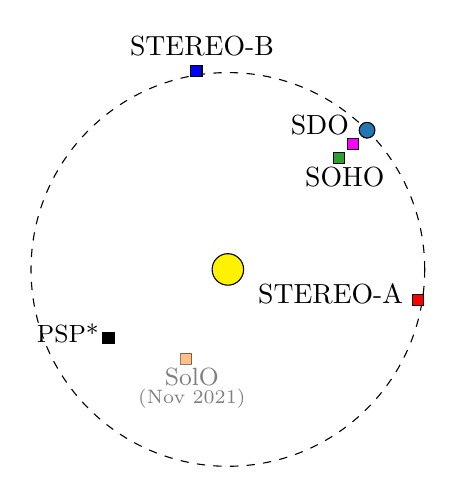
\begin{tikzpicture}
                \def\earthorbitradius{2.5}
                \def\sunradius{0.2}
                
                % sun
                \draw[fill=yellow] (0, 0) circle (\sunradius);
                
                % Earth
                \draw[dashed] (0, 0) circle (\earthorbitradius);
                \draw[fill=blue] (45:\earthorbitradius) circle (0.1);
                
                \draw[fill=Blue] ({45+54}:1.02*\earthorbitradius) +(-2pt,-2pt) rectangle +(2pt,2pt) node[above] {STEREO-B};
                \draw[fill=Red] ({45-54}:0.98*\earthorbitradius) +(-2pt,-2pt) rectangle +(2pt,2pt) node[left, xshift=-4pt] {STEREO-A};
                
                \draw[fill=Magenta] (45:0.9*\earthorbitradius) +(-2pt,-2pt) rectangle +(2pt,2pt) node[above left,yshift=-2pt] {SDO};
                \draw[fill=green] (45:0.8*\earthorbitradius) +(-2pt,-2pt) rectangle +(2pt,2pt) node[below,yshift=-2pt] {SOHO};
                
                \draw[fill=orange,opacity=0.5] (245:0.5*\earthorbitradius) +(-2pt,-2pt) rectangle +(2pt,2pt) node[below, yshift=-2pt, align=center] {\small SolO\\[-2mm]\scriptsize (Nov 2021)};
                \draw[fill=black] (210:0.7*\earthorbitradius) +(-2pt,-2pt) rectangle +(2pt,2pt) node[left, xshift=-2pt] {\small PSP*};
               
            \end{tikzpicture}
        \end{column}
        \begin{column}{0.45\textwidth}
            \textbf{In situ}\\[0.2cm]
            \centering
            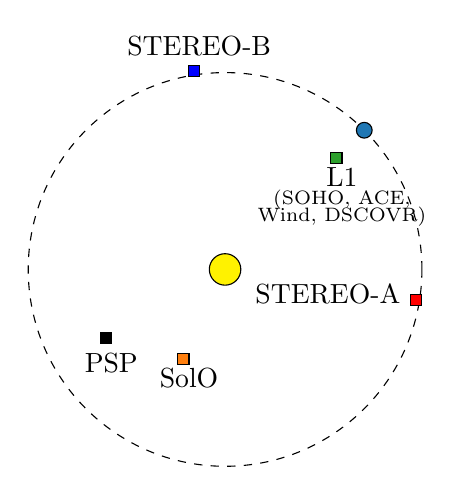
\begin{tikzpicture}
                \def\earthorbitradius{2.5}
                \def\sunradius{0.2}
                
                % sun
                \draw[fill=yellow] (0, 0) circle (\sunradius);
                
                % Earth
                \draw[dashed] (0, 0) circle (\earthorbitradius);
                \draw[fill=blue] (45:\earthorbitradius) circle (0.1);
                
                % satellites
                \draw[fill=Blue] ({45+54}:1.02*\earthorbitradius) +(-2pt,-2pt) rectangle +(2pt,2pt) node[above] {STEREO-B};
                \draw[fill=Red] ({45-54}:0.98*\earthorbitradius) +(-2pt,-2pt) rectangle +(2pt,2pt) node[left, xshift=-4pt] {STEREO-A};
                
                \draw[fill=green] (45:0.8*\earthorbitradius) +(-2pt,-2pt) rectangle +(2pt,2pt) node[below, yshift=-2pt, align=center] {L1\\[-2mm]\scriptsize (SOHO, ACE,\\[-2mm]\scriptsize Wind, DSCOVR)};                
                \draw[fill=orange] (245:0.5*\earthorbitradius) +(-2pt,-2pt) rectangle +(2pt,2pt) node[below, yshift=-2pt] {SolO};
                \draw[fill=black] (210:0.7*\earthorbitradius) +(-2pt,-2pt) rectangle +(2pt,2pt) node[below, yshift=-4pt] {PSP};
                
            \end{tikzpicture}
        \end{column}
    \end{columns}
    \begin{flushright}
        \footnotesize not to scale
    \end{flushright}
\end{frame}

\begin{frame}{Forbush decreases}
    \begin{columns}
        \begin{column}{0.55\textwidth}
            \begin{itemize}
                \item Short-term decrases of GCR intensity
                \item Discovered 1937 by Scott E. Forbush
                \item Turbulent or closed magnetic structures (ICMEs/SIRs) = barrier for GCRs
            \end{itemize}
            \uncover<2->{$\Rightarrow$ Another way to observe ICMEs in situ. Particle detectors are available at Earth, but also on many spacecraft (e.g. planetary missions)}
        \end{column}
        \begin{column}{0.35\textwidth}
            \centering
            \includegraphics[width=\textwidth]{../images/richardson_cane_2011_icme_enhanced.png}
            \footnotesize Richardson and Cane (2011)
        \end{column}
    \end{columns}
\end{frame}

\begin{frame}{FDs as additional in situ observations}
	\begin{columns}[t]
		\begin{column}{0.45\textwidth}
			\textbf{Remote sensing}\\[0.2cm]
            \centering
            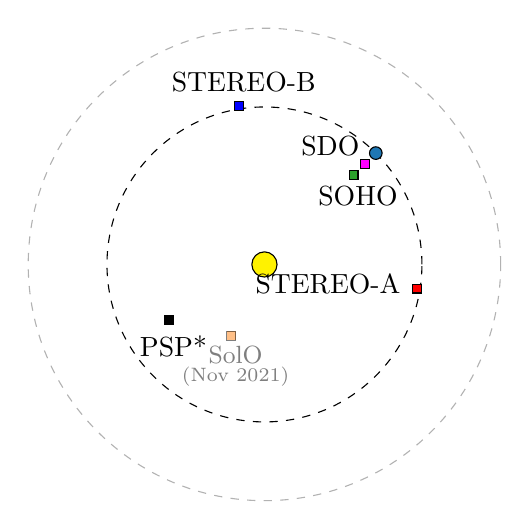
\begin{tikzpicture}[scale=0.8]
                \def\earthorbitradius{2.5}
                \def\sunradius{0.2}
                
                % sun
                \draw[fill=yellow] (0, 0) circle (\sunradius);
                
                % Earth
                \draw[dashed] (0, 0) circle (\earthorbitradius);
                \draw[fill=blue] (45:\earthorbitradius) circle (0.1);
                
                \draw[fill=Blue] ({45+54}:1.02*\earthorbitradius) +(-2pt,-2pt) rectangle +(2pt,2pt) node[above] {STEREO-B};
                \draw[fill=Red] ({45-54}:0.98*\earthorbitradius) +(-2pt,-2pt) rectangle +(2pt,2pt) node[left, xshift=-4pt] {STEREO-A};
                
                \draw[fill=Magenta] (45:0.9*\earthorbitradius) +(-2pt,-2pt) rectangle +(2pt,2pt) node[above left,yshift=-2pt] {SDO};
                \draw[fill=green] (45:0.8*\earthorbitradius) +(-2pt,-2pt) rectangle +(2pt,2pt) node[below,yshift=-2pt] {SOHO};
                
                \draw[fill=orange,opacity=0.5] (245:0.5*\earthorbitradius) +(-2pt,-2pt) rectangle +(2pt,2pt) node[below, yshift=-2pt, align=center] {\small SolO\\[-2mm]\scriptsize (Nov 2021)};
                \draw[fill=black] (210:0.7*\earthorbitradius) +(-2pt,-2pt) rectangle +(2pt,2pt) node[below, yshift=-4pt] {PSP*};
                
                \draw[dashed, opacity=0.3] (0, 0) circle (\earthorbitradius*1.5);
                
            \end{tikzpicture}
		\end{column}
		\begin{column}{0.45\textwidth}
			\textbf{In situ + FDs}\\[0.2cm]
			\centering
			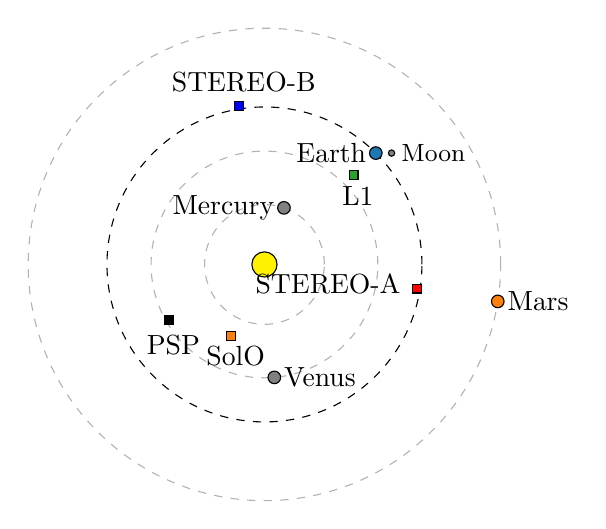
\begin{tikzpicture}[scale=0.8]
			\def\earthorbitradius{2.5}
			\def\sunradius{0.2}
			
			% sun
			\draw[fill=yellow] (0, 0) circle (\sunradius);
			
			% Earth
			\draw[dashed] (0, 0) circle (\earthorbitradius);
			\draw[fill=blue] (45:\earthorbitradius) circle (0.1) node[left] {Earth};
            
            % Moon
            \draw[fill=gray] (45:\earthorbitradius) ++ (0:\earthorbitradius*0.1) circle (0.05) node[right] {\small Moon};
			
			% Mars
			\draw[dashed, opacity=0.3] (0, 0) circle (\earthorbitradius*1.5);
			\draw[fill=orange] ({45-54}:\earthorbitradius*1.5) circle (0.1) node[right] {Mars};
			
			% Venus
			\draw[dashed, opacity=0.3] (0, 0) circle (\earthorbitradius*0.72);
			\draw[fill=gray] ({245+30}:\earthorbitradius*0.72) circle (0.1) node[right] {Venus};
			
			% Mercury
			\draw[dashed, opacity=0.3] (0, 0) circle (\earthorbitradius*0.38);
			\draw[fill=gray] ({45+26}:\earthorbitradius*0.38) circle (0.1) node[left] {Mercury};
			
			% satellites
			\draw[fill=Blue] ({45+54}:1.02*\earthorbitradius) +(-2pt,-2pt) rectangle +(2pt,2pt) node[above] {STEREO-B};
			\draw[fill=Red] ({45-54}:0.98*\earthorbitradius) +(-2pt,-2pt) rectangle +(2pt,2pt) node[left, xshift=-4pt] {STEREO-A};
			
			\draw[fill=green] (45:0.8*\earthorbitradius) +(-2pt,-2pt) rectangle +(2pt,2pt) node[below, yshift=-2pt, align=center] {L1};                
			\draw[fill=orange] (245:0.5*\earthorbitradius) +(-2pt,-2pt) rectangle +(2pt,2pt) node[below, yshift=-2pt] {SolO};
			\draw[fill=black] (210:0.7*\earthorbitradius) +(-2pt,-2pt) rectangle +(2pt,2pt) node[below, yshift=-4pt] {PSP};
			
			\end{tikzpicture}
			+ many others
		\end{column}
	\end{columns}
\end{frame}

\begin{frame}{Multipoint observations}
    \vskip0.2cm
    \begin{center}
        \includegraphics[width=0.8\linewidth]{images/witasse2017.png}\\
        \footnotesize Witasse et al. (2017)
    \end{center}
    \uncover<2->{
        \begin{quote}
            ``More information on ICME properties can probably be obtained [from] these data sets. For example, we suspect that the evolution of the radial extension of the ICME could be inferred from the Forbush decrease data.''
        \end{quote}
    }
\end{frame}

\section{Instrumentation}

\begin{frame}{Radiation Assessment Detector}
    \begin{columns}
        \begin{column}{0.50\textwidth}
            \begin{itemize}
                \item Onboard Mars Science Laboratory (\emph{Curiosity} rover)
                \item \textbf{Cruise phase:} 12/2011--07/2012,
                \textbf{surface phase} since 08/2012
                \item Data products: \textcolor{green}{charged} and \textcolor{gray}{neutral} \textbf{particle spectra} + \textbf{dosimetry} (TID, LET)
                \item \textbf{TID in E}: best statistics to observe FDs
            \end{itemize}
            %% Creator: Matplotlib, PGF backend
%%
%% To include the figure in your LaTeX document, write
%%   \input{<filename>.pgf}
%%
%% Make sure the required packages are loaded in your preamble
%%   \usepackage{pgf}
%%
%% and, on pdftex
%%   \usepackage[utf8]{inputenc}\DeclareUnicodeCharacter{2212}{-}
%%
%% or, on luatex and xetex
%%   \usepackage{unicode-math}
%%
%% Figures using additional raster images can only be included by \input if
%% they are in the same directory as the main LaTeX file. For loading figures
%% from other directories you can use the `import` package
%%   \usepackage{import}
%%
%% and then include the figures with
%%   \import{<path to file>}{<filename>.pgf}
%%
%% Matplotlib used the following preamble
%%   \usepackage{siunitx}
%%   \usepackage{fontspec}
%%
\begingroup%
\makeatletter%
\begin{pgfpicture}%
\pgfpathrectangle{\pgfpointorigin}{\pgfqpoint{3.100000in}{1.400000in}}%
\pgfusepath{use as bounding box, clip}%
\begin{pgfscope}%
\pgfsetbuttcap%
\pgfsetmiterjoin%
\definecolor{currentfill}{rgb}{1.000000,1.000000,1.000000}%
\pgfsetfillcolor{currentfill}%
\pgfsetlinewidth{0.000000pt}%
\definecolor{currentstroke}{rgb}{1.000000,1.000000,1.000000}%
\pgfsetstrokecolor{currentstroke}%
\pgfsetdash{}{0pt}%
\pgfpathmoveto{\pgfqpoint{0.000000in}{0.000000in}}%
\pgfpathlineto{\pgfqpoint{3.100000in}{0.000000in}}%
\pgfpathlineto{\pgfqpoint{3.100000in}{1.400000in}}%
\pgfpathlineto{\pgfqpoint{0.000000in}{1.400000in}}%
\pgfpathclose%
\pgfusepath{fill}%
\end{pgfscope}%
\begin{pgfscope}%
\pgfsetbuttcap%
\pgfsetmiterjoin%
\definecolor{currentfill}{rgb}{1.000000,1.000000,1.000000}%
\pgfsetfillcolor{currentfill}%
\pgfsetlinewidth{0.000000pt}%
\definecolor{currentstroke}{rgb}{0.000000,0.000000,0.000000}%
\pgfsetstrokecolor{currentstroke}%
\pgfsetstrokeopacity{0.000000}%
\pgfsetdash{}{0pt}%
\pgfpathmoveto{\pgfqpoint{0.554900in}{0.379400in}}%
\pgfpathlineto{\pgfqpoint{1.956100in}{0.379400in}}%
\pgfpathlineto{\pgfqpoint{1.956100in}{1.261400in}}%
\pgfpathlineto{\pgfqpoint{0.554900in}{1.261400in}}%
\pgfpathclose%
\pgfusepath{fill}%
\end{pgfscope}%
\begin{pgfscope}%
\pgfsetbuttcap%
\pgfsetroundjoin%
\definecolor{currentfill}{rgb}{0.000000,0.000000,0.000000}%
\pgfsetfillcolor{currentfill}%
\pgfsetlinewidth{0.803000pt}%
\definecolor{currentstroke}{rgb}{0.000000,0.000000,0.000000}%
\pgfsetstrokecolor{currentstroke}%
\pgfsetdash{}{0pt}%
\pgfsys@defobject{currentmarker}{\pgfqpoint{0.000000in}{-0.048611in}}{\pgfqpoint{0.000000in}{0.000000in}}{%
\pgfpathmoveto{\pgfqpoint{0.000000in}{0.000000in}}%
\pgfpathlineto{\pgfqpoint{0.000000in}{-0.048611in}}%
\pgfusepath{stroke,fill}%
}%
\begin{pgfscope}%
\pgfsys@transformshift{0.628433in}{0.379400in}%
\pgfsys@useobject{currentmarker}{}%
\end{pgfscope}%
\end{pgfscope}%
\begin{pgfscope}%
\definecolor{textcolor}{rgb}{0.000000,0.000000,0.000000}%
\pgfsetstrokecolor{textcolor}%
\pgfsetfillcolor{textcolor}%
\pgftext[x=0.609572in, y=0.075678in, left, base,rotate=90.000000]{\color{textcolor}\sffamily\fontsize{7.000000}{8.400000}\selectfont 2012}%
\end{pgfscope}%
\begin{pgfscope}%
\pgfsetbuttcap%
\pgfsetroundjoin%
\definecolor{currentfill}{rgb}{0.000000,0.000000,0.000000}%
\pgfsetfillcolor{currentfill}%
\pgfsetlinewidth{0.803000pt}%
\definecolor{currentstroke}{rgb}{0.000000,0.000000,0.000000}%
\pgfsetstrokecolor{currentstroke}%
\pgfsetdash{}{0pt}%
\pgfsys@defobject{currentmarker}{\pgfqpoint{0.000000in}{-0.048611in}}{\pgfqpoint{0.000000in}{0.000000in}}{%
\pgfpathmoveto{\pgfqpoint{0.000000in}{0.000000in}}%
\pgfpathlineto{\pgfqpoint{0.000000in}{-0.048611in}}%
\pgfusepath{stroke,fill}%
}%
\begin{pgfscope}%
\pgfsys@transformshift{0.778565in}{0.379400in}%
\pgfsys@useobject{currentmarker}{}%
\end{pgfscope}%
\end{pgfscope}%
\begin{pgfscope}%
\definecolor{textcolor}{rgb}{0.000000,0.000000,0.000000}%
\pgfsetstrokecolor{textcolor}%
\pgfsetfillcolor{textcolor}%
\pgftext[x=0.759704in, y=0.075678in, left, base,rotate=90.000000]{\color{textcolor}\sffamily\fontsize{7.000000}{8.400000}\selectfont 2013}%
\end{pgfscope}%
\begin{pgfscope}%
\pgfsetbuttcap%
\pgfsetroundjoin%
\definecolor{currentfill}{rgb}{0.000000,0.000000,0.000000}%
\pgfsetfillcolor{currentfill}%
\pgfsetlinewidth{0.803000pt}%
\definecolor{currentstroke}{rgb}{0.000000,0.000000,0.000000}%
\pgfsetstrokecolor{currentstroke}%
\pgfsetdash{}{0pt}%
\pgfsys@defobject{currentmarker}{\pgfqpoint{0.000000in}{-0.048611in}}{\pgfqpoint{0.000000in}{0.000000in}}{%
\pgfpathmoveto{\pgfqpoint{0.000000in}{0.000000in}}%
\pgfpathlineto{\pgfqpoint{0.000000in}{-0.048611in}}%
\pgfusepath{stroke,fill}%
}%
\begin{pgfscope}%
\pgfsys@transformshift{0.928286in}{0.379400in}%
\pgfsys@useobject{currentmarker}{}%
\end{pgfscope}%
\end{pgfscope}%
\begin{pgfscope}%
\definecolor{textcolor}{rgb}{0.000000,0.000000,0.000000}%
\pgfsetstrokecolor{textcolor}%
\pgfsetfillcolor{textcolor}%
\pgftext[x=0.909425in, y=0.075678in, left, base,rotate=90.000000]{\color{textcolor}\sffamily\fontsize{7.000000}{8.400000}\selectfont 2014}%
\end{pgfscope}%
\begin{pgfscope}%
\pgfsetbuttcap%
\pgfsetroundjoin%
\definecolor{currentfill}{rgb}{0.000000,0.000000,0.000000}%
\pgfsetfillcolor{currentfill}%
\pgfsetlinewidth{0.803000pt}%
\definecolor{currentstroke}{rgb}{0.000000,0.000000,0.000000}%
\pgfsetstrokecolor{currentstroke}%
\pgfsetdash{}{0pt}%
\pgfsys@defobject{currentmarker}{\pgfqpoint{0.000000in}{-0.048611in}}{\pgfqpoint{0.000000in}{0.000000in}}{%
\pgfpathmoveto{\pgfqpoint{0.000000in}{0.000000in}}%
\pgfpathlineto{\pgfqpoint{0.000000in}{-0.048611in}}%
\pgfusepath{stroke,fill}%
}%
\begin{pgfscope}%
\pgfsys@transformshift{1.078007in}{0.379400in}%
\pgfsys@useobject{currentmarker}{}%
\end{pgfscope}%
\end{pgfscope}%
\begin{pgfscope}%
\definecolor{textcolor}{rgb}{0.000000,0.000000,0.000000}%
\pgfsetstrokecolor{textcolor}%
\pgfsetfillcolor{textcolor}%
\pgftext[x=1.059146in, y=0.075678in, left, base,rotate=90.000000]{\color{textcolor}\sffamily\fontsize{7.000000}{8.400000}\selectfont 2015}%
\end{pgfscope}%
\begin{pgfscope}%
\pgfsetbuttcap%
\pgfsetroundjoin%
\definecolor{currentfill}{rgb}{0.000000,0.000000,0.000000}%
\pgfsetfillcolor{currentfill}%
\pgfsetlinewidth{0.803000pt}%
\definecolor{currentstroke}{rgb}{0.000000,0.000000,0.000000}%
\pgfsetstrokecolor{currentstroke}%
\pgfsetdash{}{0pt}%
\pgfsys@defobject{currentmarker}{\pgfqpoint{0.000000in}{-0.048611in}}{\pgfqpoint{0.000000in}{0.000000in}}{%
\pgfpathmoveto{\pgfqpoint{0.000000in}{0.000000in}}%
\pgfpathlineto{\pgfqpoint{0.000000in}{-0.048611in}}%
\pgfusepath{stroke,fill}%
}%
\begin{pgfscope}%
\pgfsys@transformshift{1.227728in}{0.379400in}%
\pgfsys@useobject{currentmarker}{}%
\end{pgfscope}%
\end{pgfscope}%
\begin{pgfscope}%
\definecolor{textcolor}{rgb}{0.000000,0.000000,0.000000}%
\pgfsetstrokecolor{textcolor}%
\pgfsetfillcolor{textcolor}%
\pgftext[x=1.208867in, y=0.075678in, left, base,rotate=90.000000]{\color{textcolor}\sffamily\fontsize{7.000000}{8.400000}\selectfont 2016}%
\end{pgfscope}%
\begin{pgfscope}%
\pgfsetbuttcap%
\pgfsetroundjoin%
\definecolor{currentfill}{rgb}{0.000000,0.000000,0.000000}%
\pgfsetfillcolor{currentfill}%
\pgfsetlinewidth{0.803000pt}%
\definecolor{currentstroke}{rgb}{0.000000,0.000000,0.000000}%
\pgfsetstrokecolor{currentstroke}%
\pgfsetdash{}{0pt}%
\pgfsys@defobject{currentmarker}{\pgfqpoint{0.000000in}{-0.048611in}}{\pgfqpoint{0.000000in}{0.000000in}}{%
\pgfpathmoveto{\pgfqpoint{0.000000in}{0.000000in}}%
\pgfpathlineto{\pgfqpoint{0.000000in}{-0.048611in}}%
\pgfusepath{stroke,fill}%
}%
\begin{pgfscope}%
\pgfsys@transformshift{1.377859in}{0.379400in}%
\pgfsys@useobject{currentmarker}{}%
\end{pgfscope}%
\end{pgfscope}%
\begin{pgfscope}%
\definecolor{textcolor}{rgb}{0.000000,0.000000,0.000000}%
\pgfsetstrokecolor{textcolor}%
\pgfsetfillcolor{textcolor}%
\pgftext[x=1.358998in, y=0.075678in, left, base,rotate=90.000000]{\color{textcolor}\sffamily\fontsize{7.000000}{8.400000}\selectfont 2017}%
\end{pgfscope}%
\begin{pgfscope}%
\pgfsetbuttcap%
\pgfsetroundjoin%
\definecolor{currentfill}{rgb}{0.000000,0.000000,0.000000}%
\pgfsetfillcolor{currentfill}%
\pgfsetlinewidth{0.803000pt}%
\definecolor{currentstroke}{rgb}{0.000000,0.000000,0.000000}%
\pgfsetstrokecolor{currentstroke}%
\pgfsetdash{}{0pt}%
\pgfsys@defobject{currentmarker}{\pgfqpoint{0.000000in}{-0.048611in}}{\pgfqpoint{0.000000in}{0.000000in}}{%
\pgfpathmoveto{\pgfqpoint{0.000000in}{0.000000in}}%
\pgfpathlineto{\pgfqpoint{0.000000in}{-0.048611in}}%
\pgfusepath{stroke,fill}%
}%
\begin{pgfscope}%
\pgfsys@transformshift{1.527580in}{0.379400in}%
\pgfsys@useobject{currentmarker}{}%
\end{pgfscope}%
\end{pgfscope}%
\begin{pgfscope}%
\definecolor{textcolor}{rgb}{0.000000,0.000000,0.000000}%
\pgfsetstrokecolor{textcolor}%
\pgfsetfillcolor{textcolor}%
\pgftext[x=1.508719in, y=0.075678in, left, base,rotate=90.000000]{\color{textcolor}\sffamily\fontsize{7.000000}{8.400000}\selectfont 2018}%
\end{pgfscope}%
\begin{pgfscope}%
\pgfsetbuttcap%
\pgfsetroundjoin%
\definecolor{currentfill}{rgb}{0.000000,0.000000,0.000000}%
\pgfsetfillcolor{currentfill}%
\pgfsetlinewidth{0.803000pt}%
\definecolor{currentstroke}{rgb}{0.000000,0.000000,0.000000}%
\pgfsetstrokecolor{currentstroke}%
\pgfsetdash{}{0pt}%
\pgfsys@defobject{currentmarker}{\pgfqpoint{0.000000in}{-0.048611in}}{\pgfqpoint{0.000000in}{0.000000in}}{%
\pgfpathmoveto{\pgfqpoint{0.000000in}{0.000000in}}%
\pgfpathlineto{\pgfqpoint{0.000000in}{-0.048611in}}%
\pgfusepath{stroke,fill}%
}%
\begin{pgfscope}%
\pgfsys@transformshift{1.677301in}{0.379400in}%
\pgfsys@useobject{currentmarker}{}%
\end{pgfscope}%
\end{pgfscope}%
\begin{pgfscope}%
\definecolor{textcolor}{rgb}{0.000000,0.000000,0.000000}%
\pgfsetstrokecolor{textcolor}%
\pgfsetfillcolor{textcolor}%
\pgftext[x=1.658440in, y=0.075678in, left, base,rotate=90.000000]{\color{textcolor}\sffamily\fontsize{7.000000}{8.400000}\selectfont 2019}%
\end{pgfscope}%
\begin{pgfscope}%
\pgfsetbuttcap%
\pgfsetroundjoin%
\definecolor{currentfill}{rgb}{0.000000,0.000000,0.000000}%
\pgfsetfillcolor{currentfill}%
\pgfsetlinewidth{0.803000pt}%
\definecolor{currentstroke}{rgb}{0.000000,0.000000,0.000000}%
\pgfsetstrokecolor{currentstroke}%
\pgfsetdash{}{0pt}%
\pgfsys@defobject{currentmarker}{\pgfqpoint{0.000000in}{-0.048611in}}{\pgfqpoint{0.000000in}{0.000000in}}{%
\pgfpathmoveto{\pgfqpoint{0.000000in}{0.000000in}}%
\pgfpathlineto{\pgfqpoint{0.000000in}{-0.048611in}}%
\pgfusepath{stroke,fill}%
}%
\begin{pgfscope}%
\pgfsys@transformshift{1.827022in}{0.379400in}%
\pgfsys@useobject{currentmarker}{}%
\end{pgfscope}%
\end{pgfscope}%
\begin{pgfscope}%
\definecolor{textcolor}{rgb}{0.000000,0.000000,0.000000}%
\pgfsetstrokecolor{textcolor}%
\pgfsetfillcolor{textcolor}%
\pgftext[x=1.808161in, y=0.075678in, left, base,rotate=90.000000]{\color{textcolor}\sffamily\fontsize{7.000000}{8.400000}\selectfont 2020}%
\end{pgfscope}%
\begin{pgfscope}%
\pgfsetbuttcap%
\pgfsetroundjoin%
\definecolor{currentfill}{rgb}{0.000000,0.000000,0.000000}%
\pgfsetfillcolor{currentfill}%
\pgfsetlinewidth{0.803000pt}%
\definecolor{currentstroke}{rgb}{0.000000,0.000000,0.000000}%
\pgfsetstrokecolor{currentstroke}%
\pgfsetdash{}{0pt}%
\pgfsys@defobject{currentmarker}{\pgfqpoint{-0.048611in}{0.000000in}}{\pgfqpoint{-0.000000in}{0.000000in}}{%
\pgfpathmoveto{\pgfqpoint{-0.000000in}{0.000000in}}%
\pgfpathlineto{\pgfqpoint{-0.048611in}{0.000000in}}%
\pgfusepath{stroke,fill}%
}%
\begin{pgfscope}%
\pgfsys@transformshift{0.554900in}{0.434525in}%
\pgfsys@useobject{currentmarker}{}%
\end{pgfscope}%
\end{pgfscope}%
\begin{pgfscope}%
\definecolor{textcolor}{rgb}{0.000000,0.000000,0.000000}%
\pgfsetstrokecolor{textcolor}%
\pgfsetfillcolor{textcolor}%
\pgftext[x=0.291589in, y=0.400789in, left, base]{\color{textcolor}\sffamily\fontsize{7.000000}{8.400000}\selectfont \(\displaystyle {200}\)}%
\end{pgfscope}%
\begin{pgfscope}%
\pgfsetbuttcap%
\pgfsetroundjoin%
\definecolor{currentfill}{rgb}{0.000000,0.000000,0.000000}%
\pgfsetfillcolor{currentfill}%
\pgfsetlinewidth{0.803000pt}%
\definecolor{currentstroke}{rgb}{0.000000,0.000000,0.000000}%
\pgfsetstrokecolor{currentstroke}%
\pgfsetdash{}{0pt}%
\pgfsys@defobject{currentmarker}{\pgfqpoint{-0.048611in}{0.000000in}}{\pgfqpoint{-0.000000in}{0.000000in}}{%
\pgfpathmoveto{\pgfqpoint{-0.000000in}{0.000000in}}%
\pgfpathlineto{\pgfqpoint{-0.048611in}{0.000000in}}%
\pgfusepath{stroke,fill}%
}%
\begin{pgfscope}%
\pgfsys@transformshift{0.554900in}{0.710150in}%
\pgfsys@useobject{currentmarker}{}%
\end{pgfscope}%
\end{pgfscope}%
\begin{pgfscope}%
\definecolor{textcolor}{rgb}{0.000000,0.000000,0.000000}%
\pgfsetstrokecolor{textcolor}%
\pgfsetfillcolor{textcolor}%
\pgftext[x=0.291589in, y=0.676414in, left, base]{\color{textcolor}\sffamily\fontsize{7.000000}{8.400000}\selectfont \(\displaystyle {300}\)}%
\end{pgfscope}%
\begin{pgfscope}%
\pgfsetbuttcap%
\pgfsetroundjoin%
\definecolor{currentfill}{rgb}{0.000000,0.000000,0.000000}%
\pgfsetfillcolor{currentfill}%
\pgfsetlinewidth{0.803000pt}%
\definecolor{currentstroke}{rgb}{0.000000,0.000000,0.000000}%
\pgfsetstrokecolor{currentstroke}%
\pgfsetdash{}{0pt}%
\pgfsys@defobject{currentmarker}{\pgfqpoint{-0.048611in}{0.000000in}}{\pgfqpoint{-0.000000in}{0.000000in}}{%
\pgfpathmoveto{\pgfqpoint{-0.000000in}{0.000000in}}%
\pgfpathlineto{\pgfqpoint{-0.048611in}{0.000000in}}%
\pgfusepath{stroke,fill}%
}%
\begin{pgfscope}%
\pgfsys@transformshift{0.554900in}{0.985775in}%
\pgfsys@useobject{currentmarker}{}%
\end{pgfscope}%
\end{pgfscope}%
\begin{pgfscope}%
\definecolor{textcolor}{rgb}{0.000000,0.000000,0.000000}%
\pgfsetstrokecolor{textcolor}%
\pgfsetfillcolor{textcolor}%
\pgftext[x=0.291589in, y=0.952039in, left, base]{\color{textcolor}\sffamily\fontsize{7.000000}{8.400000}\selectfont \(\displaystyle {400}\)}%
\end{pgfscope}%
\begin{pgfscope}%
\pgfsetbuttcap%
\pgfsetroundjoin%
\definecolor{currentfill}{rgb}{0.000000,0.000000,0.000000}%
\pgfsetfillcolor{currentfill}%
\pgfsetlinewidth{0.803000pt}%
\definecolor{currentstroke}{rgb}{0.000000,0.000000,0.000000}%
\pgfsetstrokecolor{currentstroke}%
\pgfsetdash{}{0pt}%
\pgfsys@defobject{currentmarker}{\pgfqpoint{-0.048611in}{0.000000in}}{\pgfqpoint{-0.000000in}{0.000000in}}{%
\pgfpathmoveto{\pgfqpoint{-0.000000in}{0.000000in}}%
\pgfpathlineto{\pgfqpoint{-0.048611in}{0.000000in}}%
\pgfusepath{stroke,fill}%
}%
\begin{pgfscope}%
\pgfsys@transformshift{0.554900in}{1.261400in}%
\pgfsys@useobject{currentmarker}{}%
\end{pgfscope}%
\end{pgfscope}%
\begin{pgfscope}%
\definecolor{textcolor}{rgb}{0.000000,0.000000,0.000000}%
\pgfsetstrokecolor{textcolor}%
\pgfsetfillcolor{textcolor}%
\pgftext[x=0.291589in, y=1.227664in, left, base]{\color{textcolor}\sffamily\fontsize{7.000000}{8.400000}\selectfont \(\displaystyle {500}\)}%
\end{pgfscope}%
\begin{pgfscope}%
\definecolor{textcolor}{rgb}{0.000000,0.000000,0.000000}%
\pgfsetstrokecolor{textcolor}%
\pgfsetfillcolor{textcolor}%
\pgftext[x=0.236033in,y=0.820400in,,bottom,rotate=90.000000]{\color{textcolor}\sffamily\fontsize{7.000000}{8.400000}\selectfont dose rate / \si{\micro\gray\per day}}%
\end{pgfscope}%
\begin{pgfscope}%
\pgfpathrectangle{\pgfqpoint{0.554900in}{0.379400in}}{\pgfqpoint{1.401200in}{0.882000in}}%
\pgfusepath{clip}%
\pgfsetrectcap%
\pgfsetroundjoin%
\pgfsetlinewidth{0.301125pt}%
\definecolor{currentstroke}{rgb}{0.121569,0.466667,0.705882}%
\pgfsetstrokecolor{currentstroke}%
\pgfsetdash{}{0pt}%
\pgfpathmoveto{\pgfqpoint{0.618591in}{0.995115in}}%
\pgfpathlineto{\pgfqpoint{0.619527in}{1.171303in}}%
\pgfpathlineto{\pgfqpoint{0.618625in}{0.972017in}}%
\pgfpathlineto{\pgfqpoint{0.619704in}{1.110454in}}%
\pgfpathlineto{\pgfqpoint{0.620099in}{0.996676in}}%
\pgfpathlineto{\pgfqpoint{0.620640in}{1.179226in}}%
\pgfpathlineto{\pgfqpoint{0.620807in}{1.073914in}}%
\pgfpathlineto{\pgfqpoint{0.621749in}{1.194028in}}%
\pgfpathlineto{\pgfqpoint{0.621124in}{1.026465in}}%
\pgfpathlineto{\pgfqpoint{0.621920in}{1.132893in}}%
\pgfpathlineto{\pgfqpoint{0.622661in}{1.034631in}}%
\pgfpathlineto{\pgfqpoint{0.622909in}{1.210508in}}%
\pgfpathlineto{\pgfqpoint{0.623034in}{1.076967in}}%
\pgfpathlineto{\pgfqpoint{0.623265in}{1.209437in}}%
\pgfpathlineto{\pgfqpoint{0.624081in}{1.016937in}}%
\pgfpathlineto{\pgfqpoint{0.624093in}{1.052988in}}%
\pgfpathlineto{\pgfqpoint{0.624371in}{1.004691in}}%
\pgfpathlineto{\pgfqpoint{0.624383in}{1.103322in}}%
\pgfpathlineto{\pgfqpoint{0.624440in}{1.073835in}}%
\pgfpathlineto{\pgfqpoint{0.625483in}{1.145740in}}%
\pgfpathlineto{\pgfqpoint{0.624449in}{0.993276in}}%
\pgfpathlineto{\pgfqpoint{0.625551in}{1.109749in}}%
\pgfpathlineto{\pgfqpoint{0.625650in}{0.987404in}}%
\pgfpathlineto{\pgfqpoint{0.625681in}{1.171344in}}%
\pgfpathlineto{\pgfqpoint{0.626554in}{1.067108in}}%
\pgfpathlineto{\pgfqpoint{0.626794in}{1.068762in}}%
\pgfpathlineto{\pgfqpoint{0.626954in}{1.186674in}}%
\pgfpathlineto{\pgfqpoint{0.627776in}{0.981342in}}%
\pgfpathlineto{\pgfqpoint{0.627897in}{1.019745in}}%
\pgfpathlineto{\pgfqpoint{0.627990in}{0.957708in}}%
\pgfpathlineto{\pgfqpoint{0.628957in}{1.148867in}}%
\pgfpathlineto{\pgfqpoint{0.628999in}{1.053810in}}%
\pgfpathlineto{\pgfqpoint{0.629152in}{1.167641in}}%
\pgfpathlineto{\pgfqpoint{0.629034in}{0.969942in}}%
\pgfpathlineto{\pgfqpoint{0.630102in}{1.034426in}}%
\pgfpathlineto{\pgfqpoint{0.630141in}{0.966167in}}%
\pgfpathlineto{\pgfqpoint{0.630532in}{1.175277in}}%
\pgfpathlineto{\pgfqpoint{0.631066in}{1.062563in}}%
\pgfpathlineto{\pgfqpoint{0.631549in}{1.211361in}}%
\pgfpathlineto{\pgfqpoint{0.631594in}{1.018655in}}%
\pgfpathlineto{\pgfqpoint{0.631888in}{1.088840in}}%
\pgfpathlineto{\pgfqpoint{0.632302in}{1.094676in}}%
\pgfpathlineto{\pgfqpoint{0.632305in}{1.060822in}}%
\pgfpathlineto{\pgfqpoint{0.632850in}{1.163084in}}%
\pgfpathlineto{\pgfqpoint{0.633002in}{1.004635in}}%
\pgfpathlineto{\pgfqpoint{0.633416in}{1.094635in}}%
\pgfpathlineto{\pgfqpoint{0.634167in}{0.994457in}}%
\pgfpathlineto{\pgfqpoint{0.634373in}{1.225254in}}%
\pgfpathlineto{\pgfqpoint{0.634527in}{1.028141in}}%
\pgfpathlineto{\pgfqpoint{0.634864in}{1.214784in}}%
\pgfpathlineto{\pgfqpoint{0.635269in}{1.000649in}}%
\pgfpathlineto{\pgfqpoint{0.635640in}{1.111782in}}%
\pgfpathlineto{\pgfqpoint{0.635962in}{1.011868in}}%
\pgfpathlineto{\pgfqpoint{0.636006in}{1.180218in}}%
\pgfpathlineto{\pgfqpoint{0.636750in}{1.150317in}}%
\pgfpathlineto{\pgfqpoint{0.637458in}{0.988862in}}%
\pgfpathlineto{\pgfqpoint{0.637645in}{1.271400in}}%
\pgfpathmoveto{\pgfqpoint{0.637645in}{1.271400in}}%
\pgfpathlineto{\pgfqpoint{0.637682in}{1.192163in}}%
\pgfpathlineto{\pgfqpoint{0.637689in}{1.271400in}}%
\pgfpathmoveto{\pgfqpoint{0.637696in}{1.271400in}}%
\pgfpathlineto{\pgfqpoint{0.637699in}{1.247905in}}%
\pgfpathlineto{\pgfqpoint{0.637705in}{1.271400in}}%
\pgfpathmoveto{\pgfqpoint{0.637709in}{1.271400in}}%
\pgfpathlineto{\pgfqpoint{0.637711in}{1.206466in}}%
\pgfpathlineto{\pgfqpoint{0.637713in}{1.271400in}}%
\pgfpathmoveto{\pgfqpoint{0.637717in}{1.271400in}}%
\pgfpathlineto{\pgfqpoint{0.637718in}{1.251145in}}%
\pgfpathlineto{\pgfqpoint{0.637720in}{1.271400in}}%
\pgfpathmoveto{\pgfqpoint{0.637721in}{1.271400in}}%
\pgfpathlineto{\pgfqpoint{0.637723in}{1.219141in}}%
\pgfpathlineto{\pgfqpoint{0.637728in}{1.271400in}}%
\pgfpathmoveto{\pgfqpoint{0.637741in}{1.271400in}}%
\pgfpathlineto{\pgfqpoint{0.637743in}{1.246792in}}%
\pgfpathlineto{\pgfqpoint{0.637746in}{1.271400in}}%
\pgfpathmoveto{\pgfqpoint{0.637807in}{1.271400in}}%
\pgfpathlineto{\pgfqpoint{0.637807in}{1.270112in}}%
\pgfpathlineto{\pgfqpoint{0.637807in}{1.271400in}}%
\pgfpathmoveto{\pgfqpoint{0.637833in}{1.271400in}}%
\pgfpathlineto{\pgfqpoint{0.637834in}{1.250350in}}%
\pgfpathlineto{\pgfqpoint{0.637835in}{1.271400in}}%
\pgfpathmoveto{\pgfqpoint{0.637845in}{1.271400in}}%
\pgfpathlineto{\pgfqpoint{0.637851in}{1.228835in}}%
\pgfpathlineto{\pgfqpoint{0.637854in}{1.271400in}}%
\pgfpathmoveto{\pgfqpoint{0.637861in}{1.271400in}}%
\pgfpathlineto{\pgfqpoint{0.637861in}{1.269291in}}%
\pgfpathlineto{\pgfqpoint{0.637861in}{1.271400in}}%
\pgfpathmoveto{\pgfqpoint{0.637864in}{1.271400in}}%
\pgfpathlineto{\pgfqpoint{0.637868in}{1.195246in}}%
\pgfpathlineto{\pgfqpoint{0.637870in}{1.271400in}}%
\pgfpathmoveto{\pgfqpoint{0.637876in}{1.271400in}}%
\pgfpathlineto{\pgfqpoint{0.637888in}{1.189911in}}%
\pgfpathlineto{\pgfqpoint{0.637901in}{1.271400in}}%
\pgfpathmoveto{\pgfqpoint{0.637903in}{1.271400in}}%
\pgfpathlineto{\pgfqpoint{0.638543in}{0.881886in}}%
\pgfpathlineto{\pgfqpoint{0.639021in}{0.971189in}}%
\pgfpathlineto{\pgfqpoint{0.639204in}{0.921673in}}%
\pgfpathlineto{\pgfqpoint{0.639422in}{1.271400in}}%
\pgfpathmoveto{\pgfqpoint{0.640148in}{1.271400in}}%
\pgfpathlineto{\pgfqpoint{0.640153in}{1.254106in}}%
\pgfpathlineto{\pgfqpoint{0.640161in}{1.271400in}}%
\pgfpathmoveto{\pgfqpoint{0.640163in}{1.271400in}}%
\pgfpathlineto{\pgfqpoint{0.640190in}{1.216821in}}%
\pgfpathlineto{\pgfqpoint{0.640198in}{1.271400in}}%
\pgfpathmoveto{\pgfqpoint{0.640201in}{1.271400in}}%
\pgfpathlineto{\pgfqpoint{0.641306in}{1.040909in}}%
\pgfpathlineto{\pgfqpoint{0.641356in}{1.082881in}}%
\pgfpathlineto{\pgfqpoint{0.642537in}{1.183993in}}%
\pgfpathlineto{\pgfqpoint{0.641587in}{0.975711in}}%
\pgfpathlineto{\pgfqpoint{0.642546in}{1.148697in}}%
\pgfpathlineto{\pgfqpoint{0.648175in}{1.096740in}}%
\pgfpathlineto{\pgfqpoint{0.648184in}{1.098565in}}%
\pgfpathlineto{\pgfqpoint{0.648545in}{1.195055in}}%
\pgfpathlineto{\pgfqpoint{0.648323in}{1.086397in}}%
\pgfpathlineto{\pgfqpoint{0.649298in}{1.139161in}}%
\pgfpathlineto{\pgfqpoint{0.649400in}{1.084320in}}%
\pgfpathlineto{\pgfqpoint{0.649996in}{1.204629in}}%
\pgfpathlineto{\pgfqpoint{0.650273in}{1.168579in}}%
\pgfpathlineto{\pgfqpoint{0.650789in}{1.227990in}}%
\pgfpathlineto{\pgfqpoint{0.650628in}{1.119004in}}%
\pgfpathlineto{\pgfqpoint{0.651384in}{1.214716in}}%
\pgfpathlineto{\pgfqpoint{0.652464in}{1.009844in}}%
\pgfpathlineto{\pgfqpoint{0.651683in}{1.226257in}}%
\pgfpathlineto{\pgfqpoint{0.652519in}{1.016037in}}%
\pgfpathlineto{\pgfqpoint{0.652556in}{1.015203in}}%
\pgfpathlineto{\pgfqpoint{0.653651in}{1.149708in}}%
\pgfpathlineto{\pgfqpoint{0.653947in}{1.072244in}}%
\pgfpathlineto{\pgfqpoint{0.654490in}{1.182343in}}%
\pgfpathlineto{\pgfqpoint{0.654758in}{1.109963in}}%
\pgfpathlineto{\pgfqpoint{0.655357in}{1.078429in}}%
\pgfpathlineto{\pgfqpoint{0.655567in}{1.271400in}}%
\pgfpathmoveto{\pgfqpoint{0.657036in}{1.271400in}}%
\pgfpathlineto{\pgfqpoint{0.658132in}{0.848250in}}%
\pgfpathlineto{\pgfqpoint{0.658193in}{0.877185in}}%
\pgfpathlineto{\pgfqpoint{0.658202in}{0.838227in}}%
\pgfpathlineto{\pgfqpoint{0.658273in}{1.271400in}}%
\pgfpathmoveto{\pgfqpoint{0.658394in}{1.271400in}}%
\pgfpathlineto{\pgfqpoint{0.658396in}{1.252321in}}%
\pgfpathlineto{\pgfqpoint{0.658407in}{1.271400in}}%
\pgfpathmoveto{\pgfqpoint{0.658422in}{1.271400in}}%
\pgfpathlineto{\pgfqpoint{0.659423in}{0.903237in}}%
\pgfpathlineto{\pgfqpoint{0.659700in}{0.950028in}}%
\pgfpathlineto{\pgfqpoint{0.659796in}{0.938208in}}%
\pgfpathlineto{\pgfqpoint{0.660400in}{1.032838in}}%
\pgfpathlineto{\pgfqpoint{0.660548in}{0.996709in}}%
\pgfpathlineto{\pgfqpoint{0.661612in}{1.064288in}}%
\pgfpathlineto{\pgfqpoint{0.660792in}{0.955777in}}%
\pgfpathlineto{\pgfqpoint{0.661677in}{1.047777in}}%
\pgfpathlineto{\pgfqpoint{0.661797in}{0.984139in}}%
\pgfpathlineto{\pgfqpoint{0.662161in}{1.113891in}}%
\pgfpathlineto{\pgfqpoint{0.662751in}{1.088513in}}%
\pgfpathlineto{\pgfqpoint{0.663726in}{1.159289in}}%
\pgfpathlineto{\pgfqpoint{0.662889in}{1.043602in}}%
\pgfpathlineto{\pgfqpoint{0.663854in}{1.092003in}}%
\pgfpathlineto{\pgfqpoint{0.664650in}{1.055664in}}%
\pgfpathlineto{\pgfqpoint{0.664530in}{1.149588in}}%
\pgfpathlineto{\pgfqpoint{0.664931in}{1.097273in}}%
\pgfpathlineto{\pgfqpoint{0.664968in}{1.150160in}}%
\pgfpathlineto{\pgfqpoint{0.665156in}{1.033434in}}%
\pgfpathlineto{\pgfqpoint{0.666032in}{1.076761in}}%
\pgfpathlineto{\pgfqpoint{0.666646in}{1.031461in}}%
\pgfpathlineto{\pgfqpoint{0.667085in}{1.133419in}}%
\pgfpathlineto{\pgfqpoint{0.667141in}{1.062214in}}%
\pgfpathlineto{\pgfqpoint{0.667665in}{1.144778in}}%
\pgfpathlineto{\pgfqpoint{0.668232in}{1.018378in}}%
\pgfpathlineto{\pgfqpoint{0.668279in}{0.997716in}}%
\pgfpathlineto{\pgfqpoint{0.668735in}{1.113862in}}%
\pgfpathlineto{\pgfqpoint{0.668979in}{1.065652in}}%
\pgfpathlineto{\pgfqpoint{0.670053in}{1.129877in}}%
\pgfpathlineto{\pgfqpoint{0.668997in}{1.040779in}}%
\pgfpathlineto{\pgfqpoint{0.670090in}{1.083386in}}%
\pgfpathlineto{\pgfqpoint{0.671048in}{1.161758in}}%
\pgfpathlineto{\pgfqpoint{0.670182in}{1.051016in}}%
\pgfpathlineto{\pgfqpoint{0.671205in}{1.133280in}}%
\pgfpathlineto{\pgfqpoint{0.671514in}{1.091010in}}%
\pgfpathlineto{\pgfqpoint{0.671850in}{1.189386in}}%
\pgfpathlineto{\pgfqpoint{0.672307in}{1.143943in}}%
\pgfpathlineto{\pgfqpoint{0.673070in}{1.208490in}}%
\pgfpathlineto{\pgfqpoint{0.672589in}{1.100067in}}%
\pgfpathlineto{\pgfqpoint{0.673420in}{1.148392in}}%
\pgfpathlineto{\pgfqpoint{0.674465in}{1.089102in}}%
\pgfpathlineto{\pgfqpoint{0.674012in}{1.226930in}}%
\pgfpathlineto{\pgfqpoint{0.674492in}{1.139304in}}%
\pgfpathlineto{\pgfqpoint{0.674642in}{1.187085in}}%
\pgfpathlineto{\pgfqpoint{0.675204in}{1.067821in}}%
\pgfpathlineto{\pgfqpoint{0.675586in}{1.131024in}}%
\pgfpathlineto{\pgfqpoint{0.676078in}{1.031139in}}%
\pgfpathlineto{\pgfqpoint{0.676682in}{1.134674in}}%
\pgfpathlineto{\pgfqpoint{0.676701in}{1.088625in}}%
\pgfpathlineto{\pgfqpoint{0.676825in}{1.051993in}}%
\pgfpathlineto{\pgfqpoint{0.677553in}{1.169443in}}%
\pgfpathlineto{\pgfqpoint{0.677729in}{1.120166in}}%
\pgfpathlineto{\pgfqpoint{0.678329in}{1.201085in}}%
\pgfpathlineto{\pgfqpoint{0.678080in}{1.094121in}}%
\pgfpathlineto{\pgfqpoint{0.678842in}{1.144153in}}%
\pgfpathlineto{\pgfqpoint{0.678953in}{1.259434in}}%
\pgfpathlineto{\pgfqpoint{0.679820in}{1.132952in}}%
\pgfpathlineto{\pgfqpoint{0.679952in}{1.201482in}}%
\pgfpathlineto{\pgfqpoint{0.679971in}{1.142933in}}%
\pgfpathlineto{\pgfqpoint{0.680975in}{1.271400in}}%
\pgfpathmoveto{\pgfqpoint{0.680976in}{1.271400in}}%
\pgfpathlineto{\pgfqpoint{0.681031in}{1.142808in}}%
\pgfpathlineto{\pgfqpoint{0.682092in}{1.213038in}}%
\pgfpathlineto{\pgfqpoint{0.682201in}{1.166770in}}%
\pgfpathlineto{\pgfqpoint{0.682210in}{1.271400in}}%
\pgfpathmoveto{\pgfqpoint{0.682211in}{1.271400in}}%
\pgfpathlineto{\pgfqpoint{0.682613in}{1.131991in}}%
\pgfpathlineto{\pgfqpoint{0.683337in}{1.175089in}}%
\pgfpathlineto{\pgfqpoint{0.683965in}{1.257935in}}%
\pgfpathlineto{\pgfqpoint{0.683808in}{1.144809in}}%
\pgfpathlineto{\pgfqpoint{0.684455in}{1.200820in}}%
\pgfpathlineto{\pgfqpoint{0.684539in}{1.111450in}}%
\pgfpathlineto{\pgfqpoint{0.684666in}{1.271400in}}%
\pgfpathmoveto{\pgfqpoint{0.685281in}{1.271400in}}%
\pgfpathlineto{\pgfqpoint{0.685285in}{1.254674in}}%
\pgfpathlineto{\pgfqpoint{0.685291in}{1.271400in}}%
\pgfpathmoveto{\pgfqpoint{0.685309in}{1.271400in}}%
\pgfpathlineto{\pgfqpoint{0.685313in}{1.253023in}}%
\pgfpathlineto{\pgfqpoint{0.685325in}{1.271400in}}%
\pgfpathmoveto{\pgfqpoint{0.685334in}{1.271400in}}%
\pgfpathlineto{\pgfqpoint{0.685340in}{1.218209in}}%
\pgfpathlineto{\pgfqpoint{0.685347in}{1.271400in}}%
\pgfpathmoveto{\pgfqpoint{0.685363in}{1.271400in}}%
\pgfpathlineto{\pgfqpoint{0.686235in}{1.152166in}}%
\pgfpathlineto{\pgfqpoint{0.686488in}{1.213702in}}%
\pgfpathlineto{\pgfqpoint{0.686737in}{1.239430in}}%
\pgfpathlineto{\pgfqpoint{0.687185in}{1.140475in}}%
\pgfpathlineto{\pgfqpoint{0.687240in}{1.187555in}}%
\pgfpathlineto{\pgfqpoint{0.687792in}{1.131135in}}%
\pgfpathlineto{\pgfqpoint{0.687802in}{1.202626in}}%
\pgfpathlineto{\pgfqpoint{0.687885in}{1.198106in}}%
\pgfpathlineto{\pgfqpoint{0.688156in}{1.253987in}}%
\pgfpathlineto{\pgfqpoint{0.688968in}{1.142780in}}%
\pgfpathlineto{\pgfqpoint{0.688986in}{1.212512in}}%
\pgfpathlineto{\pgfqpoint{0.690055in}{1.122233in}}%
\pgfpathlineto{\pgfqpoint{0.689023in}{1.230376in}}%
\pgfpathlineto{\pgfqpoint{0.690120in}{1.153306in}}%
\pgfpathlineto{\pgfqpoint{0.691115in}{1.221390in}}%
\pgfpathlineto{\pgfqpoint{0.690166in}{1.122288in}}%
\pgfpathlineto{\pgfqpoint{0.691235in}{1.170660in}}%
\pgfpathlineto{\pgfqpoint{0.692106in}{1.047931in}}%
\pgfpathlineto{\pgfqpoint{0.691558in}{1.199031in}}%
\pgfpathlineto{\pgfqpoint{0.692355in}{1.070228in}}%
\pgfpathlineto{\pgfqpoint{0.692621in}{1.140106in}}%
\pgfpathlineto{\pgfqpoint{0.692520in}{1.037146in}}%
\pgfpathlineto{\pgfqpoint{0.692769in}{1.066999in}}%
\pgfpathlineto{\pgfqpoint{0.694007in}{1.097355in}}%
\pgfpathlineto{\pgfqpoint{0.694208in}{1.160458in}}%
\pgfpathlineto{\pgfqpoint{0.694494in}{1.065534in}}%
\pgfpathlineto{\pgfqpoint{0.694670in}{1.116300in}}%
\pgfpathlineto{\pgfqpoint{0.695799in}{1.213258in}}%
\pgfpathlineto{\pgfqpoint{0.695550in}{1.114176in}}%
\pgfpathlineto{\pgfqpoint{0.695867in}{1.143746in}}%
\pgfpathlineto{\pgfqpoint{0.696826in}{1.117295in}}%
\pgfpathlineto{\pgfqpoint{0.696789in}{1.213781in}}%
\pgfpathlineto{\pgfqpoint{0.696955in}{1.174751in}}%
\pgfpathlineto{\pgfqpoint{0.697011in}{1.134165in}}%
\pgfpathlineto{\pgfqpoint{0.697421in}{1.226888in}}%
\pgfpathlineto{\pgfqpoint{0.697720in}{1.180316in}}%
\pgfpathlineto{\pgfqpoint{0.697766in}{1.229460in}}%
\pgfpathlineto{\pgfqpoint{0.698532in}{1.068737in}}%
\pgfpathlineto{\pgfqpoint{0.698821in}{1.136137in}}%
\pgfpathlineto{\pgfqpoint{0.698932in}{1.070625in}}%
\pgfpathlineto{\pgfqpoint{0.699518in}{1.196408in}}%
\pgfpathlineto{\pgfqpoint{0.699919in}{1.148841in}}%
\pgfpathlineto{\pgfqpoint{0.700647in}{1.190166in}}%
\pgfpathlineto{\pgfqpoint{0.700826in}{1.095702in}}%
\pgfpathlineto{\pgfqpoint{0.701020in}{1.129732in}}%
\pgfpathlineto{\pgfqpoint{0.701066in}{1.196516in}}%
\pgfpathlineto{\pgfqpoint{0.701649in}{1.100317in}}%
\pgfpathlineto{\pgfqpoint{0.702140in}{1.181093in}}%
\pgfpathlineto{\pgfqpoint{0.702251in}{1.103316in}}%
\pgfpathlineto{\pgfqpoint{0.703145in}{1.202461in}}%
\pgfpathlineto{\pgfqpoint{0.703250in}{1.171414in}}%
\pgfpathlineto{\pgfqpoint{0.703565in}{1.094265in}}%
\pgfpathlineto{\pgfqpoint{0.703670in}{1.214654in}}%
\pgfpathlineto{\pgfqpoint{0.704348in}{1.108185in}}%
\pgfpathlineto{\pgfqpoint{0.705131in}{1.210623in}}%
\pgfpathlineto{\pgfqpoint{0.704993in}{1.072546in}}%
\pgfpathlineto{\pgfqpoint{0.705459in}{1.138082in}}%
\pgfpathlineto{\pgfqpoint{0.705970in}{1.070664in}}%
\pgfpathlineto{\pgfqpoint{0.706445in}{1.181952in}}%
\pgfpathlineto{\pgfqpoint{0.706569in}{1.132477in}}%
\pgfpathlineto{\pgfqpoint{0.707248in}{1.164958in}}%
\pgfpathlineto{\pgfqpoint{0.706970in}{1.055609in}}%
\pgfpathlineto{\pgfqpoint{0.707667in}{1.101267in}}%
\pgfpathlineto{\pgfqpoint{0.707694in}{1.059501in}}%
\pgfpathlineto{\pgfqpoint{0.707920in}{1.192003in}}%
\pgfpathlineto{\pgfqpoint{0.708422in}{1.129032in}}%
\pgfusepath{stroke}%
\end{pgfscope}%
\begin{pgfscope}%
\pgfpathrectangle{\pgfqpoint{0.554900in}{0.379400in}}{\pgfqpoint{1.401200in}{0.882000in}}%
\pgfusepath{clip}%
\pgfsetrectcap%
\pgfsetroundjoin%
\pgfsetlinewidth{0.301125pt}%
\definecolor{currentstroke}{rgb}{1.000000,0.498039,0.054902}%
\pgfsetstrokecolor{currentstroke}%
\pgfsetdash{}{0pt}%
\pgfpathmoveto{\pgfqpoint{0.718310in}{0.445820in}}%
\pgfpathlineto{\pgfqpoint{0.719207in}{0.418557in}}%
\pgfpathlineto{\pgfqpoint{0.718348in}{0.471978in}}%
\pgfpathlineto{\pgfqpoint{0.719216in}{0.445138in}}%
\pgfpathlineto{\pgfqpoint{0.721689in}{0.448862in}}%
\pgfpathlineto{\pgfqpoint{0.722137in}{0.459953in}}%
\pgfpathlineto{\pgfqpoint{0.722538in}{0.369400in}}%
\pgfpathmoveto{\pgfqpoint{0.722574in}{0.369400in}}%
\pgfpathlineto{\pgfqpoint{0.722595in}{0.465523in}}%
\pgfpathlineto{\pgfqpoint{0.722946in}{0.369400in}}%
\pgfpathmoveto{\pgfqpoint{0.722981in}{0.369400in}}%
\pgfpathlineto{\pgfqpoint{0.723881in}{0.469813in}}%
\pgfpathlineto{\pgfqpoint{0.724089in}{0.451284in}}%
\pgfpathlineto{\pgfqpoint{0.724717in}{0.480467in}}%
\pgfpathlineto{\pgfqpoint{0.724520in}{0.440198in}}%
\pgfpathlineto{\pgfqpoint{0.725213in}{0.469946in}}%
\pgfpathlineto{\pgfqpoint{0.726185in}{0.433151in}}%
\pgfpathlineto{\pgfqpoint{0.725241in}{0.472745in}}%
\pgfpathlineto{\pgfqpoint{0.726326in}{0.452653in}}%
\pgfpathlineto{\pgfqpoint{0.727269in}{0.461880in}}%
\pgfpathlineto{\pgfqpoint{0.726662in}{0.420702in}}%
\pgfpathlineto{\pgfqpoint{0.727354in}{0.446183in}}%
\pgfpathlineto{\pgfqpoint{0.727969in}{0.428680in}}%
\pgfpathlineto{\pgfqpoint{0.728170in}{0.468876in}}%
\pgfpathlineto{\pgfqpoint{0.728436in}{0.458158in}}%
\pgfpathlineto{\pgfqpoint{0.729396in}{0.487977in}}%
\pgfpathlineto{\pgfqpoint{0.728756in}{0.439690in}}%
\pgfpathlineto{\pgfqpoint{0.729556in}{0.466605in}}%
\pgfpathlineto{\pgfqpoint{0.729585in}{0.456000in}}%
\pgfpathlineto{\pgfqpoint{0.729707in}{0.485761in}}%
\pgfpathlineto{\pgfqpoint{0.729751in}{0.472311in}}%
\pgfpathlineto{\pgfqpoint{0.732227in}{0.465211in}}%
\pgfpathlineto{\pgfqpoint{0.732243in}{0.465893in}}%
\pgfpathlineto{\pgfqpoint{0.732533in}{0.443544in}}%
\pgfpathlineto{\pgfqpoint{0.733139in}{0.482460in}}%
\pgfpathlineto{\pgfqpoint{0.733358in}{0.458979in}}%
\pgfpathlineto{\pgfqpoint{0.733555in}{0.480255in}}%
\pgfpathlineto{\pgfqpoint{0.734179in}{0.435913in}}%
\pgfpathlineto{\pgfqpoint{0.734437in}{0.458925in}}%
\pgfpathlineto{\pgfqpoint{0.734693in}{0.438470in}}%
\pgfpathlineto{\pgfqpoint{0.735231in}{0.483598in}}%
\pgfpathlineto{\pgfqpoint{0.735533in}{0.462198in}}%
\pgfpathlineto{\pgfqpoint{0.736593in}{0.488427in}}%
\pgfpathlineto{\pgfqpoint{0.735920in}{0.447796in}}%
\pgfpathlineto{\pgfqpoint{0.736659in}{0.469818in}}%
\pgfpathlineto{\pgfqpoint{0.737138in}{0.453346in}}%
\pgfpathlineto{\pgfqpoint{0.737383in}{0.497237in}}%
\pgfpathlineto{\pgfqpoint{0.737721in}{0.480582in}}%
\pgfpathlineto{\pgfqpoint{0.737796in}{0.491072in}}%
\pgfpathlineto{\pgfqpoint{0.738720in}{0.442124in}}%
\pgfpathlineto{\pgfqpoint{0.738777in}{0.443247in}}%
\pgfpathlineto{\pgfqpoint{0.739520in}{0.400837in}}%
\pgfpathlineto{\pgfqpoint{0.739068in}{0.470153in}}%
\pgfpathlineto{\pgfqpoint{0.739900in}{0.422696in}}%
\pgfpathlineto{\pgfqpoint{0.740769in}{0.456464in}}%
\pgfpathlineto{\pgfqpoint{0.740145in}{0.408375in}}%
\pgfpathlineto{\pgfqpoint{0.741061in}{0.451940in}}%
\pgfpathlineto{\pgfqpoint{0.742157in}{0.414046in}}%
\pgfpathlineto{\pgfqpoint{0.741526in}{0.458829in}}%
\pgfpathlineto{\pgfqpoint{0.742204in}{0.425065in}}%
\pgfpathlineto{\pgfqpoint{0.743302in}{0.458435in}}%
\pgfpathlineto{\pgfqpoint{0.742232in}{0.419992in}}%
\pgfpathlineto{\pgfqpoint{0.743340in}{0.448656in}}%
\pgfpathlineto{\pgfqpoint{0.743886in}{0.412317in}}%
\pgfpathlineto{\pgfqpoint{0.744414in}{0.455235in}}%
\pgfpathlineto{\pgfqpoint{0.744423in}{0.443326in}}%
\pgfpathlineto{\pgfqpoint{0.745284in}{0.434160in}}%
\pgfpathlineto{\pgfqpoint{0.746122in}{0.458598in}}%
\pgfpathlineto{\pgfqpoint{0.746376in}{0.419989in}}%
\pgfpathlineto{\pgfqpoint{0.746386in}{0.427281in}}%
\pgfpathlineto{\pgfqpoint{0.747398in}{0.458985in}}%
\pgfpathlineto{\pgfqpoint{0.746814in}{0.419033in}}%
\pgfpathlineto{\pgfqpoint{0.747527in}{0.451728in}}%
\pgfpathlineto{\pgfqpoint{0.748523in}{0.420335in}}%
\pgfpathlineto{\pgfqpoint{0.748326in}{0.470873in}}%
\pgfpathlineto{\pgfqpoint{0.748674in}{0.444514in}}%
\pgfpathlineto{\pgfqpoint{0.749089in}{0.458012in}}%
\pgfpathlineto{\pgfqpoint{0.749424in}{0.424082in}}%
\pgfpathlineto{\pgfqpoint{0.749773in}{0.436466in}}%
\pgfpathlineto{\pgfqpoint{0.749782in}{0.431048in}}%
\pgfpathlineto{\pgfqpoint{0.750484in}{0.467912in}}%
\pgfpathlineto{\pgfqpoint{0.750832in}{0.459121in}}%
\pgfpathlineto{\pgfqpoint{0.751624in}{0.481621in}}%
\pgfpathlineto{\pgfqpoint{0.751021in}{0.434783in}}%
\pgfpathlineto{\pgfqpoint{0.751897in}{0.449429in}}%
\pgfpathlineto{\pgfqpoint{0.752281in}{0.429916in}}%
\pgfpathlineto{\pgfqpoint{0.752121in}{0.464688in}}%
\pgfpathlineto{\pgfqpoint{0.753003in}{0.439907in}}%
\pgfpathlineto{\pgfqpoint{0.753795in}{0.464208in}}%
\pgfpathlineto{\pgfqpoint{0.753116in}{0.425636in}}%
\pgfpathlineto{\pgfqpoint{0.754112in}{0.443139in}}%
\pgfpathlineto{\pgfqpoint{0.755007in}{0.472829in}}%
\pgfpathlineto{\pgfqpoint{0.754451in}{0.431370in}}%
\pgfpathlineto{\pgfqpoint{0.755195in}{0.446186in}}%
\pgfpathlineto{\pgfqpoint{0.755631in}{0.433886in}}%
\pgfpathlineto{\pgfqpoint{0.756254in}{0.476397in}}%
\pgfpathlineto{\pgfqpoint{0.756264in}{0.469429in}}%
\pgfpathlineto{\pgfqpoint{0.757196in}{0.485240in}}%
\pgfpathlineto{\pgfqpoint{0.756565in}{0.446968in}}%
\pgfpathlineto{\pgfqpoint{0.757366in}{0.466480in}}%
\pgfpathlineto{\pgfqpoint{0.758040in}{0.490096in}}%
\pgfpathlineto{\pgfqpoint{0.757451in}{0.456583in}}%
\pgfpathlineto{\pgfqpoint{0.758483in}{0.472753in}}%
\pgfpathlineto{\pgfqpoint{0.758705in}{0.417583in}}%
\pgfpathlineto{\pgfqpoint{0.759619in}{0.446548in}}%
\pgfpathlineto{\pgfqpoint{0.759675in}{0.465537in}}%
\pgfpathlineto{\pgfqpoint{0.760408in}{0.419669in}}%
\pgfpathlineto{\pgfqpoint{0.760709in}{0.435519in}}%
\pgfpathlineto{\pgfqpoint{0.761600in}{0.418161in}}%
\pgfpathlineto{\pgfqpoint{0.760945in}{0.477157in}}%
\pgfpathlineto{\pgfqpoint{0.761822in}{0.432291in}}%
\pgfpathlineto{\pgfqpoint{0.762697in}{0.454050in}}%
\pgfpathlineto{\pgfqpoint{0.761991in}{0.402736in}}%
\pgfpathlineto{\pgfqpoint{0.762933in}{0.436637in}}%
\pgfpathlineto{\pgfqpoint{0.763444in}{0.464546in}}%
\pgfpathlineto{\pgfqpoint{0.763294in}{0.431837in}}%
\pgfpathlineto{\pgfqpoint{0.764066in}{0.448565in}}%
\pgfpathlineto{\pgfqpoint{0.764104in}{0.426618in}}%
\pgfpathlineto{\pgfqpoint{0.765116in}{0.487493in}}%
\pgfpathlineto{\pgfqpoint{0.765163in}{0.463872in}}%
\pgfpathlineto{\pgfqpoint{0.766066in}{0.482424in}}%
\pgfpathlineto{\pgfqpoint{0.765446in}{0.442844in}}%
\pgfpathlineto{\pgfqpoint{0.766241in}{0.453862in}}%
\pgfpathlineto{\pgfqpoint{0.766661in}{0.439815in}}%
\pgfpathlineto{\pgfqpoint{0.766426in}{0.486684in}}%
\pgfpathlineto{\pgfqpoint{0.767344in}{0.459968in}}%
\pgfpathlineto{\pgfqpoint{0.767746in}{0.484770in}}%
\pgfpathlineto{\pgfqpoint{0.767504in}{0.446706in}}%
\pgfpathlineto{\pgfqpoint{0.768471in}{0.476553in}}%
\pgfpathlineto{\pgfqpoint{0.769613in}{0.442098in}}%
\pgfpathlineto{\pgfqpoint{0.768555in}{0.485228in}}%
\pgfpathlineto{\pgfqpoint{0.769641in}{0.455538in}}%
\pgfpathlineto{\pgfqpoint{0.770254in}{0.482262in}}%
\pgfpathlineto{\pgfqpoint{0.769670in}{0.444299in}}%
\pgfpathlineto{\pgfqpoint{0.770743in}{0.457635in}}%
\pgfpathlineto{\pgfqpoint{0.771764in}{0.437685in}}%
\pgfpathlineto{\pgfqpoint{0.771086in}{0.479007in}}%
\pgfpathlineto{\pgfqpoint{0.771839in}{0.452895in}}%
\pgfpathlineto{\pgfqpoint{0.771924in}{0.486335in}}%
\pgfpathlineto{\pgfqpoint{0.772927in}{0.429153in}}%
\pgfpathlineto{\pgfqpoint{0.772936in}{0.442175in}}%
\pgfpathlineto{\pgfqpoint{0.773436in}{0.431057in}}%
\pgfpathlineto{\pgfqpoint{0.773618in}{0.472236in}}%
\pgfpathlineto{\pgfqpoint{0.773973in}{0.465839in}}%
\pgfpathlineto{\pgfqpoint{0.774001in}{0.482556in}}%
\pgfpathlineto{\pgfqpoint{0.774186in}{0.444641in}}%
\pgfpathlineto{\pgfqpoint{0.775065in}{0.460295in}}%
\pgfpathlineto{\pgfqpoint{0.775140in}{0.447976in}}%
\pgfpathlineto{\pgfqpoint{0.775263in}{0.491755in}}%
\pgfpathlineto{\pgfqpoint{0.776143in}{0.475795in}}%
\pgfpathlineto{\pgfqpoint{0.776153in}{0.489206in}}%
\pgfpathlineto{\pgfqpoint{0.777091in}{0.440857in}}%
\pgfpathlineto{\pgfqpoint{0.777232in}{0.452066in}}%
\pgfpathlineto{\pgfqpoint{0.777242in}{0.443418in}}%
\pgfpathlineto{\pgfqpoint{0.778256in}{0.479824in}}%
\pgfpathlineto{\pgfqpoint{0.778313in}{0.476294in}}%
\pgfpathlineto{\pgfqpoint{0.778680in}{0.493173in}}%
\pgfpathlineto{\pgfqpoint{0.778876in}{0.447632in}}%
\pgfpathlineto{\pgfqpoint{0.779378in}{0.455723in}}%
\pgfpathlineto{\pgfqpoint{0.779387in}{0.448117in}}%
\pgfpathlineto{\pgfqpoint{0.780350in}{0.489585in}}%
\pgfpathlineto{\pgfqpoint{0.780473in}{0.465544in}}%
\pgfpathlineto{\pgfqpoint{0.780482in}{0.465639in}}%
\pgfpathlineto{\pgfqpoint{0.780605in}{0.456872in}}%
\pgfpathlineto{\pgfqpoint{0.780642in}{0.459058in}}%
\pgfpathlineto{\pgfqpoint{0.781038in}{0.450447in}}%
\pgfpathlineto{\pgfqpoint{0.781634in}{0.495774in}}%
\pgfpathlineto{\pgfqpoint{0.781690in}{0.472153in}}%
\pgfpathlineto{\pgfqpoint{0.782472in}{0.501713in}}%
\pgfpathlineto{\pgfqpoint{0.781851in}{0.460327in}}%
\pgfpathlineto{\pgfqpoint{0.782811in}{0.488784in}}%
\pgfpathlineto{\pgfqpoint{0.783509in}{0.455361in}}%
\pgfpathlineto{\pgfqpoint{0.783273in}{0.502587in}}%
\pgfpathlineto{\pgfqpoint{0.783933in}{0.473757in}}%
\pgfpathlineto{\pgfqpoint{0.784309in}{0.450537in}}%
\pgfpathlineto{\pgfqpoint{0.784102in}{0.490193in}}%
\pgfpathlineto{\pgfqpoint{0.785049in}{0.468337in}}%
\pgfpathlineto{\pgfqpoint{0.785846in}{0.491529in}}%
\pgfpathlineto{\pgfqpoint{0.785215in}{0.449854in}}%
\pgfpathlineto{\pgfqpoint{0.786185in}{0.487432in}}%
\pgfpathlineto{\pgfqpoint{0.786452in}{0.458864in}}%
\pgfpathlineto{\pgfqpoint{0.787149in}{0.501637in}}%
\pgfpathlineto{\pgfqpoint{0.787309in}{0.474981in}}%
\pgfpathlineto{\pgfqpoint{0.787516in}{0.503807in}}%
\pgfpathlineto{\pgfqpoint{0.788025in}{0.461353in}}%
\pgfpathlineto{\pgfqpoint{0.788406in}{0.491062in}}%
\pgfpathlineto{\pgfqpoint{0.789065in}{0.455715in}}%
\pgfpathlineto{\pgfqpoint{0.788773in}{0.493679in}}%
\pgfpathlineto{\pgfqpoint{0.789520in}{0.470409in}}%
\pgfpathlineto{\pgfqpoint{0.789614in}{0.498440in}}%
\pgfpathlineto{\pgfqpoint{0.789840in}{0.454655in}}%
\pgfpathlineto{\pgfqpoint{0.790579in}{0.482487in}}%
\pgfpathlineto{\pgfqpoint{0.790701in}{0.450423in}}%
\pgfpathlineto{\pgfqpoint{0.791677in}{0.495776in}}%
\pgfpathlineto{\pgfqpoint{0.792421in}{0.461931in}}%
\pgfpathlineto{\pgfqpoint{0.792177in}{0.500227in}}%
\pgfpathlineto{\pgfqpoint{0.792864in}{0.472266in}}%
\pgfpathlineto{\pgfqpoint{0.793367in}{0.500047in}}%
\pgfpathlineto{\pgfqpoint{0.793263in}{0.460202in}}%
\pgfpathlineto{\pgfqpoint{0.793985in}{0.478619in}}%
\pgfpathlineto{\pgfqpoint{0.794088in}{0.466261in}}%
\pgfpathlineto{\pgfqpoint{0.794238in}{0.498365in}}%
\pgfpathlineto{\pgfqpoint{0.794266in}{0.488118in}}%
\pgfpathlineto{\pgfqpoint{0.794275in}{0.502917in}}%
\pgfpathlineto{\pgfqpoint{0.795342in}{0.458504in}}%
\pgfpathlineto{\pgfqpoint{0.795360in}{0.472541in}}%
\pgfpathlineto{\pgfqpoint{0.796390in}{0.497973in}}%
\pgfpathlineto{\pgfqpoint{0.795772in}{0.459592in}}%
\pgfpathlineto{\pgfqpoint{0.796483in}{0.481617in}}%
\pgfpathlineto{\pgfqpoint{0.796568in}{0.458824in}}%
\pgfpathlineto{\pgfqpoint{0.796826in}{0.498142in}}%
\pgfpathlineto{\pgfqpoint{0.797579in}{0.490793in}}%
\pgfpathlineto{\pgfqpoint{0.798418in}{0.510946in}}%
\pgfpathlineto{\pgfqpoint{0.798625in}{0.465992in}}%
\pgfpathlineto{\pgfqpoint{0.798644in}{0.473269in}}%
\pgfpathlineto{\pgfqpoint{0.799558in}{0.456021in}}%
\pgfpathlineto{\pgfqpoint{0.798804in}{0.488872in}}%
\pgfpathlineto{\pgfqpoint{0.799719in}{0.486577in}}%
\pgfpathlineto{\pgfqpoint{0.800605in}{0.504849in}}%
\pgfpathlineto{\pgfqpoint{0.800351in}{0.465223in}}%
\pgfpathlineto{\pgfqpoint{0.800794in}{0.475441in}}%
\pgfpathlineto{\pgfqpoint{0.800822in}{0.458061in}}%
\pgfpathlineto{\pgfqpoint{0.801471in}{0.497764in}}%
\pgfpathlineto{\pgfqpoint{0.801848in}{0.484694in}}%
\pgfpathlineto{\pgfqpoint{0.802281in}{0.501571in}}%
\pgfpathlineto{\pgfqpoint{0.802130in}{0.460265in}}%
\pgfpathlineto{\pgfqpoint{0.802536in}{0.475065in}}%
\pgfpathlineto{\pgfqpoint{0.805552in}{0.484074in}}%
\pgfpathlineto{\pgfqpoint{0.805675in}{0.506169in}}%
\pgfpathlineto{\pgfqpoint{0.806278in}{0.372634in}}%
\pgfpathlineto{\pgfqpoint{0.806604in}{0.417988in}}%
\pgfpathlineto{\pgfqpoint{0.806680in}{0.408938in}}%
\pgfpathlineto{\pgfqpoint{0.807787in}{0.454528in}}%
\pgfpathlineto{\pgfqpoint{0.807929in}{0.423347in}}%
\pgfpathlineto{\pgfqpoint{0.808576in}{0.460273in}}%
\pgfpathlineto{\pgfqpoint{0.811467in}{0.463719in}}%
\pgfpathlineto{\pgfqpoint{0.811976in}{0.492124in}}%
\pgfpathlineto{\pgfqpoint{0.812134in}{0.455371in}}%
\pgfpathlineto{\pgfqpoint{0.812567in}{0.465700in}}%
\pgfpathlineto{\pgfqpoint{0.812602in}{0.451193in}}%
\pgfpathlineto{\pgfqpoint{0.813181in}{0.484816in}}%
\pgfpathlineto{\pgfqpoint{0.813665in}{0.457865in}}%
\pgfpathlineto{\pgfqpoint{0.814534in}{0.471860in}}%
\pgfpathlineto{\pgfqpoint{0.813822in}{0.450055in}}%
\pgfpathlineto{\pgfqpoint{0.814762in}{0.456990in}}%
\pgfpathlineto{\pgfqpoint{0.814938in}{0.468886in}}%
\pgfpathlineto{\pgfqpoint{0.815209in}{0.447486in}}%
\pgfpathlineto{\pgfqpoint{0.815490in}{0.451010in}}%
\pgfpathlineto{\pgfqpoint{0.815595in}{0.441214in}}%
\pgfpathlineto{\pgfqpoint{0.816117in}{0.468622in}}%
\pgfpathlineto{\pgfqpoint{0.816521in}{0.455020in}}%
\pgfpathlineto{\pgfqpoint{0.817439in}{0.475208in}}%
\pgfpathlineto{\pgfqpoint{0.816802in}{0.434416in}}%
\pgfpathlineto{\pgfqpoint{0.817615in}{0.451116in}}%
\pgfpathlineto{\pgfqpoint{0.817667in}{0.441863in}}%
\pgfpathlineto{\pgfqpoint{0.817808in}{0.460552in}}%
\pgfpathlineto{\pgfqpoint{0.818734in}{0.482287in}}%
\pgfpathlineto{\pgfqpoint{0.818576in}{0.449883in}}%
\pgfpathlineto{\pgfqpoint{0.818909in}{0.463988in}}%
\pgfpathlineto{\pgfqpoint{0.819371in}{0.446697in}}%
\pgfpathlineto{\pgfqpoint{0.819733in}{0.485943in}}%
\pgfpathlineto{\pgfqpoint{0.819838in}{0.600962in}}%
\pgfpathlineto{\pgfqpoint{0.820609in}{0.448833in}}%
\pgfpathlineto{\pgfqpoint{0.820832in}{0.470605in}}%
\pgfpathlineto{\pgfqpoint{0.821691in}{0.480711in}}%
\pgfpathlineto{\pgfqpoint{0.821060in}{0.448525in}}%
\pgfpathlineto{\pgfqpoint{0.821830in}{0.472251in}}%
\pgfpathlineto{\pgfqpoint{0.821900in}{0.455933in}}%
\pgfpathlineto{\pgfqpoint{0.822076in}{0.486956in}}%
\pgfpathlineto{\pgfqpoint{0.822918in}{0.485416in}}%
\pgfpathlineto{\pgfqpoint{0.824051in}{0.450116in}}%
\pgfpathlineto{\pgfqpoint{0.824068in}{0.462669in}}%
\pgfpathlineto{\pgfqpoint{0.824209in}{0.475686in}}%
\pgfpathlineto{\pgfqpoint{0.824384in}{0.445575in}}%
\pgfpathlineto{\pgfqpoint{0.825109in}{0.463762in}}%
\pgfpathlineto{\pgfqpoint{0.825670in}{0.441088in}}%
\pgfpathlineto{\pgfqpoint{0.825425in}{0.468929in}}%
\pgfpathlineto{\pgfqpoint{0.826232in}{0.457237in}}%
\pgfpathlineto{\pgfqpoint{0.826355in}{0.467792in}}%
\pgfpathlineto{\pgfqpoint{0.826908in}{0.414597in}}%
\pgfpathlineto{\pgfqpoint{0.826978in}{0.416775in}}%
\pgfpathlineto{\pgfqpoint{0.827793in}{0.403380in}}%
\pgfpathlineto{\pgfqpoint{0.827153in}{0.430906in}}%
\pgfpathlineto{\pgfqpoint{0.828074in}{0.415283in}}%
\pgfpathlineto{\pgfqpoint{0.828302in}{0.422997in}}%
\pgfpathlineto{\pgfqpoint{0.828162in}{0.403741in}}%
\pgfpathlineto{\pgfqpoint{0.828329in}{0.404673in}}%
\pgfpathlineto{\pgfqpoint{0.830526in}{0.461871in}}%
\pgfpathlineto{\pgfqpoint{0.830714in}{0.433585in}}%
\pgfpathlineto{\pgfqpoint{0.830827in}{0.423280in}}%
\pgfpathlineto{\pgfqpoint{0.831709in}{0.461126in}}%
\pgfpathlineto{\pgfqpoint{0.831793in}{0.460389in}}%
\pgfpathlineto{\pgfqpoint{0.832001in}{0.439778in}}%
\pgfpathlineto{\pgfqpoint{0.832641in}{0.485901in}}%
\pgfpathlineto{\pgfqpoint{0.832896in}{0.462147in}}%
\pgfpathlineto{\pgfqpoint{0.833018in}{0.485545in}}%
\pgfpathlineto{\pgfqpoint{0.833630in}{0.438397in}}%
\pgfpathlineto{\pgfqpoint{0.833979in}{0.447640in}}%
\pgfpathlineto{\pgfqpoint{0.834527in}{0.432774in}}%
\pgfpathlineto{\pgfqpoint{0.834725in}{0.471972in}}%
\pgfpathlineto{\pgfqpoint{0.835065in}{0.455750in}}%
\pgfpathlineto{\pgfqpoint{0.835121in}{0.473082in}}%
\pgfpathlineto{\pgfqpoint{0.835328in}{0.435902in}}%
\pgfpathlineto{\pgfqpoint{0.835686in}{0.446592in}}%
\pgfpathlineto{\pgfqpoint{0.836685in}{0.423801in}}%
\pgfpathlineto{\pgfqpoint{0.836748in}{0.465403in}}%
\pgfpathlineto{\pgfqpoint{0.836767in}{0.459341in}}%
\pgfpathlineto{\pgfqpoint{0.836842in}{0.471047in}}%
\pgfpathlineto{\pgfqpoint{0.837822in}{0.438612in}}%
\pgfpathlineto{\pgfqpoint{0.837832in}{0.445717in}}%
\pgfpathlineto{\pgfqpoint{0.837963in}{0.422164in}}%
\pgfpathlineto{\pgfqpoint{0.838556in}{0.456900in}}%
\pgfpathlineto{\pgfqpoint{0.838943in}{0.434066in}}%
\pgfpathlineto{\pgfqpoint{0.839084in}{0.450732in}}%
\pgfpathlineto{\pgfqpoint{0.839593in}{0.414292in}}%
\pgfpathlineto{\pgfqpoint{0.840035in}{0.420104in}}%
\pgfpathlineto{\pgfqpoint{0.840892in}{0.406739in}}%
\pgfpathlineto{\pgfqpoint{0.840214in}{0.443408in}}%
\pgfpathlineto{\pgfqpoint{0.841043in}{0.431279in}}%
\pgfpathlineto{\pgfqpoint{0.841900in}{0.452117in}}%
\pgfpathlineto{\pgfqpoint{0.841259in}{0.405472in}}%
\pgfpathlineto{\pgfqpoint{0.842145in}{0.429303in}}%
\pgfpathlineto{\pgfqpoint{0.842927in}{0.413355in}}%
\pgfpathlineto{\pgfqpoint{0.842305in}{0.446097in}}%
\pgfpathlineto{\pgfqpoint{0.843068in}{0.430601in}}%
\pgfpathlineto{\pgfqpoint{0.844019in}{0.453955in}}%
\pgfpathlineto{\pgfqpoint{0.843322in}{0.419493in}}%
\pgfpathlineto{\pgfqpoint{0.844189in}{0.437173in}}%
\pgfpathlineto{\pgfqpoint{0.844198in}{0.426284in}}%
\pgfpathlineto{\pgfqpoint{0.844566in}{0.467407in}}%
\pgfpathlineto{\pgfqpoint{0.845277in}{0.455216in}}%
\pgfpathlineto{\pgfqpoint{0.845654in}{0.470275in}}%
\pgfpathlineto{\pgfqpoint{0.846247in}{0.424915in}}%
\pgfpathlineto{\pgfqpoint{0.846360in}{0.427375in}}%
\pgfpathlineto{\pgfqpoint{0.846369in}{0.422626in}}%
\pgfpathlineto{\pgfqpoint{0.847340in}{0.455079in}}%
\pgfpathlineto{\pgfqpoint{0.847415in}{0.445660in}}%
\pgfpathlineto{\pgfqpoint{0.848216in}{0.463208in}}%
\pgfpathlineto{\pgfqpoint{0.847943in}{0.428393in}}%
\pgfpathlineto{\pgfqpoint{0.848536in}{0.452770in}}%
\pgfpathlineto{\pgfqpoint{0.848635in}{0.483082in}}%
\pgfpathlineto{\pgfqpoint{0.848912in}{0.438180in}}%
\pgfpathlineto{\pgfqpoint{0.849248in}{0.447084in}}%
\pgfpathlineto{\pgfqpoint{0.850128in}{0.412664in}}%
\pgfpathlineto{\pgfqpoint{0.849822in}{0.468739in}}%
\pgfpathlineto{\pgfqpoint{0.850357in}{0.434246in}}%
\pgfpathlineto{\pgfqpoint{0.851152in}{0.469638in}}%
\pgfpathlineto{\pgfqpoint{0.850459in}{0.416684in}}%
\pgfpathlineto{\pgfqpoint{0.851468in}{0.450258in}}%
\pgfpathlineto{\pgfqpoint{0.851643in}{0.476507in}}%
\pgfpathlineto{\pgfqpoint{0.852593in}{0.419508in}}%
\pgfpathlineto{\pgfqpoint{0.853693in}{0.467580in}}%
\pgfpathlineto{\pgfqpoint{0.853512in}{0.413505in}}%
\pgfpathlineto{\pgfqpoint{0.853713in}{0.464187in}}%
\pgfpathlineto{\pgfqpoint{0.854700in}{0.424462in}}%
\pgfpathlineto{\pgfqpoint{0.854501in}{0.475378in}}%
\pgfpathlineto{\pgfqpoint{0.854826in}{0.434426in}}%
\pgfpathlineto{\pgfqpoint{0.855434in}{0.471828in}}%
\pgfpathlineto{\pgfqpoint{0.855658in}{0.422967in}}%
\pgfpathlineto{\pgfqpoint{0.855935in}{0.446881in}}%
\pgfpathlineto{\pgfqpoint{0.855940in}{0.425131in}}%
\pgfpathlineto{\pgfqpoint{0.856606in}{0.478508in}}%
\pgfpathlineto{\pgfqpoint{0.857042in}{0.456443in}}%
\pgfpathlineto{\pgfqpoint{0.857067in}{0.483914in}}%
\pgfpathlineto{\pgfqpoint{0.857290in}{0.428981in}}%
\pgfpathlineto{\pgfqpoint{0.858146in}{0.448142in}}%
\pgfpathlineto{\pgfqpoint{0.858890in}{0.435471in}}%
\pgfpathlineto{\pgfqpoint{0.858778in}{0.489213in}}%
\pgfpathlineto{\pgfqpoint{0.859235in}{0.459888in}}%
\pgfpathlineto{\pgfqpoint{0.859594in}{0.493797in}}%
\pgfpathlineto{\pgfqpoint{0.859828in}{0.434698in}}%
\pgfpathlineto{\pgfqpoint{0.860348in}{0.462005in}}%
\pgfpathlineto{\pgfqpoint{0.861456in}{0.428302in}}%
\pgfpathlineto{\pgfqpoint{0.860435in}{0.485429in}}%
\pgfpathlineto{\pgfqpoint{0.861461in}{0.436136in}}%
\pgfpathlineto{\pgfqpoint{0.862069in}{0.525575in}}%
\pgfpathlineto{\pgfqpoint{0.861938in}{0.426227in}}%
\pgfpathlineto{\pgfqpoint{0.862581in}{0.467446in}}%
\pgfpathlineto{\pgfqpoint{0.862722in}{0.437848in}}%
\pgfpathlineto{\pgfqpoint{0.862999in}{0.489043in}}%
\pgfpathlineto{\pgfqpoint{0.863695in}{0.452627in}}%
\pgfpathlineto{\pgfqpoint{0.863739in}{0.465816in}}%
\pgfpathlineto{\pgfqpoint{0.864001in}{0.408711in}}%
\pgfpathlineto{\pgfqpoint{0.864794in}{0.428668in}}%
\pgfpathlineto{\pgfqpoint{0.864862in}{0.413246in}}%
\pgfpathlineto{\pgfqpoint{0.865467in}{0.472942in}}%
\pgfpathlineto{\pgfqpoint{0.865696in}{0.449986in}}%
\pgfpathlineto{\pgfqpoint{0.865983in}{0.482021in}}%
\pgfpathlineto{\pgfqpoint{0.865739in}{0.430071in}}%
\pgfpathlineto{\pgfqpoint{0.866817in}{0.475832in}}%
\pgfpathlineto{\pgfqpoint{0.867857in}{0.441571in}}%
\pgfpathlineto{\pgfqpoint{0.867911in}{0.490572in}}%
\pgfpathlineto{\pgfqpoint{0.867930in}{0.457805in}}%
\pgfpathlineto{\pgfqpoint{0.868037in}{0.479669in}}%
\pgfpathlineto{\pgfqpoint{0.868689in}{0.430346in}}%
\pgfpathlineto{\pgfqpoint{0.869033in}{0.453765in}}%
\pgfpathlineto{\pgfqpoint{0.869125in}{0.431075in}}%
\pgfpathlineto{\pgfqpoint{0.869660in}{0.493915in}}%
\pgfpathlineto{\pgfqpoint{0.870121in}{0.469184in}}%
\pgfpathlineto{\pgfqpoint{0.870620in}{0.484160in}}%
\pgfpathlineto{\pgfqpoint{0.870763in}{0.426267in}}%
\pgfpathlineto{\pgfqpoint{0.871222in}{0.450106in}}%
\pgfpathlineto{\pgfqpoint{0.871605in}{0.418111in}}%
\pgfpathlineto{\pgfqpoint{0.872198in}{0.475093in}}%
\pgfpathlineto{\pgfqpoint{0.872339in}{0.442800in}}%
\pgfpathlineto{\pgfqpoint{0.872647in}{0.475086in}}%
\pgfpathlineto{\pgfqpoint{0.872763in}{0.428345in}}%
\pgfpathlineto{\pgfqpoint{0.873463in}{0.465259in}}%
\pgfpathlineto{\pgfqpoint{0.873513in}{0.480516in}}%
\pgfpathlineto{\pgfqpoint{0.873671in}{0.438564in}}%
\pgfpathlineto{\pgfqpoint{0.874441in}{0.447905in}}%
\pgfpathlineto{\pgfqpoint{0.875453in}{0.418533in}}%
\pgfpathlineto{\pgfqpoint{0.875178in}{0.470281in}}%
\pgfpathlineto{\pgfqpoint{0.875547in}{0.449569in}}%
\pgfpathlineto{\pgfqpoint{0.876430in}{0.472555in}}%
\pgfpathlineto{\pgfqpoint{0.875874in}{0.410412in}}%
\pgfpathlineto{\pgfqpoint{0.876515in}{0.444090in}}%
\pgfpathlineto{\pgfqpoint{0.876635in}{0.415746in}}%
\pgfpathlineto{\pgfqpoint{0.877298in}{0.468075in}}%
\pgfpathlineto{\pgfqpoint{0.877616in}{0.447760in}}%
\pgfpathlineto{\pgfqpoint{0.878388in}{0.484690in}}%
\pgfpathlineto{\pgfqpoint{0.878326in}{0.439955in}}%
\pgfpathlineto{\pgfqpoint{0.878722in}{0.445014in}}%
\pgfpathlineto{\pgfqpoint{0.878833in}{0.476470in}}%
\pgfpathlineto{\pgfqpoint{0.879214in}{0.432234in}}%
\pgfpathlineto{\pgfqpoint{0.879696in}{0.448099in}}%
\pgfpathlineto{\pgfqpoint{0.880356in}{0.420753in}}%
\pgfpathlineto{\pgfqpoint{0.879856in}{0.484592in}}%
\pgfpathlineto{\pgfqpoint{0.880807in}{0.431104in}}%
\pgfpathlineto{\pgfqpoint{0.881541in}{0.471152in}}%
\pgfpathlineto{\pgfqpoint{0.881744in}{0.423277in}}%
\pgfpathlineto{\pgfqpoint{0.881925in}{0.453741in}}%
\pgfpathlineto{\pgfqpoint{0.882208in}{0.427705in}}%
\pgfpathlineto{\pgfqpoint{0.882782in}{0.468224in}}%
\pgfpathlineto{\pgfqpoint{0.883045in}{0.444439in}}%
\pgfpathlineto{\pgfqpoint{0.884056in}{0.478674in}}%
\pgfpathlineto{\pgfqpoint{0.883467in}{0.426745in}}%
\pgfpathlineto{\pgfqpoint{0.884158in}{0.449109in}}%
\pgfpathlineto{\pgfqpoint{0.884501in}{0.476640in}}%
\pgfpathlineto{\pgfqpoint{0.884252in}{0.429469in}}%
\pgfpathlineto{\pgfqpoint{0.885266in}{0.461169in}}%
\pgfpathlineto{\pgfqpoint{0.885816in}{0.485331in}}%
\pgfpathlineto{\pgfqpoint{0.886383in}{0.424344in}}%
\pgfpathlineto{\pgfqpoint{0.887429in}{0.481167in}}%
\pgfpathlineto{\pgfqpoint{0.887496in}{0.450282in}}%
\pgfpathlineto{\pgfqpoint{0.887858in}{0.483045in}}%
\pgfpathlineto{\pgfqpoint{0.888534in}{0.437260in}}%
\pgfpathlineto{\pgfqpoint{0.888607in}{0.451164in}}%
\pgfpathlineto{\pgfqpoint{0.889482in}{0.501226in}}%
\pgfpathlineto{\pgfqpoint{0.888934in}{0.436872in}}%
\pgfpathlineto{\pgfqpoint{0.889734in}{0.471358in}}%
\pgfpathlineto{\pgfqpoint{0.890540in}{0.444863in}}%
\pgfpathlineto{\pgfqpoint{0.890322in}{0.485749in}}%
\pgfpathlineto{\pgfqpoint{0.890842in}{0.464124in}}%
\pgfpathlineto{\pgfqpoint{0.891201in}{0.490239in}}%
\pgfpathlineto{\pgfqpoint{0.890975in}{0.442064in}}%
\pgfpathlineto{\pgfqpoint{0.891948in}{0.463650in}}%
\pgfpathlineto{\pgfqpoint{0.892320in}{0.452914in}}%
\pgfpathlineto{\pgfqpoint{0.892042in}{0.498699in}}%
\pgfpathlineto{\pgfqpoint{0.893018in}{0.472908in}}%
\pgfpathlineto{\pgfqpoint{0.893712in}{0.494976in}}%
\pgfpathlineto{\pgfqpoint{0.893106in}{0.451191in}}%
\pgfpathlineto{\pgfqpoint{0.894126in}{0.484731in}}%
\pgfpathlineto{\pgfqpoint{0.894751in}{0.435168in}}%
\pgfpathlineto{\pgfqpoint{0.894835in}{0.974026in}}%
\pgfpathlineto{\pgfqpoint{0.895229in}{0.478393in}}%
\pgfpathlineto{\pgfqpoint{0.895404in}{0.502707in}}%
\pgfpathlineto{\pgfqpoint{0.895986in}{0.451370in}}%
\pgfpathlineto{\pgfqpoint{0.896341in}{0.487908in}}%
\pgfpathlineto{\pgfqpoint{0.897420in}{0.453805in}}%
\pgfpathlineto{\pgfqpoint{0.896436in}{0.503934in}}%
\pgfpathlineto{\pgfqpoint{0.897454in}{0.463068in}}%
\pgfpathlineto{\pgfqpoint{0.897575in}{0.504645in}}%
\pgfpathlineto{\pgfqpoint{0.897731in}{0.453376in}}%
\pgfpathlineto{\pgfqpoint{0.898569in}{0.472539in}}%
\pgfpathlineto{\pgfqpoint{0.899105in}{0.450206in}}%
\pgfpathlineto{\pgfqpoint{0.898816in}{0.507884in}}%
\pgfpathlineto{\pgfqpoint{0.899676in}{0.468914in}}%
\pgfpathlineto{\pgfqpoint{0.900463in}{0.498393in}}%
\pgfpathlineto{\pgfqpoint{0.900312in}{0.448647in}}%
\pgfpathlineto{\pgfqpoint{0.900775in}{0.450718in}}%
\pgfpathlineto{\pgfqpoint{0.901428in}{0.501260in}}%
\pgfpathlineto{\pgfqpoint{0.901035in}{0.442215in}}%
\pgfpathlineto{\pgfqpoint{0.901906in}{0.464855in}}%
\pgfpathlineto{\pgfqpoint{0.902435in}{0.444760in}}%
\pgfpathlineto{\pgfqpoint{0.902244in}{0.491207in}}%
\pgfpathlineto{\pgfqpoint{0.902996in}{0.472697in}}%
\pgfpathlineto{\pgfqpoint{0.904108in}{0.445911in}}%
\pgfpathlineto{\pgfqpoint{0.903438in}{0.494392in}}%
\pgfpathlineto{\pgfqpoint{0.904134in}{0.449658in}}%
\pgfpathlineto{\pgfqpoint{0.904188in}{0.471419in}}%
\pgfpathlineto{\pgfqpoint{0.904915in}{0.402203in}}%
\pgfpathlineto{\pgfqpoint{0.904999in}{0.416829in}}%
\pgfpathlineto{\pgfqpoint{0.908809in}{0.451882in}}%
\pgfpathlineto{\pgfqpoint{0.908817in}{0.451748in}}%
\pgfpathlineto{\pgfqpoint{0.908901in}{0.488043in}}%
\pgfpathlineto{\pgfqpoint{0.909531in}{0.421246in}}%
\pgfpathlineto{\pgfqpoint{0.909918in}{0.452786in}}%
\pgfpathlineto{\pgfqpoint{0.910356in}{0.433563in}}%
\pgfpathlineto{\pgfqpoint{0.910011in}{0.469850in}}%
\pgfpathlineto{\pgfqpoint{0.910493in}{0.461835in}}%
\pgfpathlineto{\pgfqpoint{0.912601in}{0.443009in}}%
\pgfpathlineto{\pgfqpoint{0.912606in}{0.449870in}}%
\pgfpathlineto{\pgfqpoint{0.913103in}{0.477505in}}%
\pgfpathlineto{\pgfqpoint{0.912939in}{0.429463in}}%
\pgfpathlineto{\pgfqpoint{0.913695in}{0.433787in}}%
\pgfpathlineto{\pgfqpoint{0.913700in}{0.433769in}}%
\pgfpathlineto{\pgfqpoint{0.914699in}{0.469407in}}%
\pgfpathlineto{\pgfqpoint{0.914141in}{0.423499in}}%
\pgfpathlineto{\pgfqpoint{0.914823in}{0.457981in}}%
\pgfpathlineto{\pgfqpoint{0.915396in}{0.421218in}}%
\pgfpathlineto{\pgfqpoint{0.915237in}{0.469074in}}%
\pgfpathlineto{\pgfqpoint{0.915937in}{0.443056in}}%
\pgfpathlineto{\pgfqpoint{0.916954in}{0.493212in}}%
\pgfpathlineto{\pgfqpoint{0.916614in}{0.440500in}}%
\pgfpathlineto{\pgfqpoint{0.917066in}{0.457178in}}%
\pgfpathlineto{\pgfqpoint{0.918019in}{0.423067in}}%
\pgfpathlineto{\pgfqpoint{0.917341in}{0.485409in}}%
\pgfpathlineto{\pgfqpoint{0.918141in}{0.449065in}}%
\pgfpathlineto{\pgfqpoint{0.918671in}{0.474618in}}%
\pgfpathlineto{\pgfqpoint{0.918808in}{0.425775in}}%
\pgfpathlineto{\pgfqpoint{0.919243in}{0.444883in}}%
\pgfpathlineto{\pgfqpoint{0.919309in}{0.434693in}}%
\pgfpathlineto{\pgfqpoint{0.919382in}{0.461847in}}%
\pgfpathlineto{\pgfqpoint{0.919386in}{0.459665in}}%
\pgfpathlineto{\pgfqpoint{0.922293in}{0.430232in}}%
\pgfpathlineto{\pgfqpoint{0.923239in}{0.462653in}}%
\pgfpathlineto{\pgfqpoint{0.922515in}{0.415314in}}%
\pgfpathlineto{\pgfqpoint{0.923406in}{0.438295in}}%
\pgfpathlineto{\pgfqpoint{0.924065in}{0.468206in}}%
\pgfpathlineto{\pgfqpoint{0.924229in}{0.424381in}}%
\pgfpathlineto{\pgfqpoint{0.924518in}{0.444113in}}%
\pgfpathlineto{\pgfqpoint{0.924689in}{0.423362in}}%
\pgfpathlineto{\pgfqpoint{0.925347in}{0.484009in}}%
\pgfpathlineto{\pgfqpoint{0.925627in}{0.432163in}}%
\pgfpathlineto{\pgfqpoint{0.925749in}{0.470986in}}%
\pgfpathlineto{\pgfqpoint{0.925886in}{0.415399in}}%
\pgfpathlineto{\pgfqpoint{0.926740in}{0.435662in}}%
\pgfpathlineto{\pgfqpoint{0.927030in}{0.481388in}}%
\pgfpathlineto{\pgfqpoint{0.926829in}{0.414299in}}%
\pgfpathlineto{\pgfqpoint{0.927879in}{0.451167in}}%
\pgfpathlineto{\pgfqpoint{0.928055in}{0.419926in}}%
\pgfpathlineto{\pgfqpoint{0.928290in}{0.483579in}}%
\pgfpathlineto{\pgfqpoint{0.928993in}{0.448591in}}%
\pgfpathlineto{\pgfqpoint{0.929075in}{0.480850in}}%
\pgfpathlineto{\pgfqpoint{0.929855in}{0.427025in}}%
\pgfpathlineto{\pgfqpoint{0.930102in}{0.453466in}}%
\pgfpathlineto{\pgfqpoint{0.931029in}{0.430831in}}%
\pgfpathlineto{\pgfqpoint{0.930557in}{0.589898in}}%
\pgfpathlineto{\pgfqpoint{0.931210in}{0.454299in}}%
\pgfpathlineto{\pgfqpoint{0.931986in}{0.473162in}}%
\pgfpathlineto{\pgfqpoint{0.931372in}{0.426630in}}%
\pgfpathlineto{\pgfqpoint{0.932317in}{0.455490in}}%
\pgfpathlineto{\pgfqpoint{0.932771in}{0.398196in}}%
\pgfpathlineto{\pgfqpoint{0.932327in}{0.461937in}}%
\pgfpathlineto{\pgfqpoint{0.933466in}{0.416797in}}%
\pgfpathlineto{\pgfqpoint{0.934440in}{0.403062in}}%
\pgfpathlineto{\pgfqpoint{0.934135in}{0.451136in}}%
\pgfpathlineto{\pgfqpoint{0.934530in}{0.418060in}}%
\pgfpathlineto{\pgfqpoint{0.935408in}{0.471753in}}%
\pgfpathlineto{\pgfqpoint{0.934870in}{0.407129in}}%
\pgfpathlineto{\pgfqpoint{0.935653in}{0.448703in}}%
\pgfpathlineto{\pgfqpoint{0.936131in}{0.426868in}}%
\pgfpathlineto{\pgfqpoint{0.935927in}{0.471412in}}%
\pgfpathlineto{\pgfqpoint{0.936752in}{0.457766in}}%
\pgfpathlineto{\pgfqpoint{0.937529in}{0.476688in}}%
\pgfpathlineto{\pgfqpoint{0.937398in}{0.431886in}}%
\pgfpathlineto{\pgfqpoint{0.937858in}{0.466305in}}%
\pgfpathlineto{\pgfqpoint{0.938200in}{0.433368in}}%
\pgfpathlineto{\pgfqpoint{0.938360in}{0.487562in}}%
\pgfpathlineto{\pgfqpoint{0.938971in}{0.455038in}}%
\pgfpathlineto{\pgfqpoint{0.939912in}{0.432084in}}%
\pgfpathlineto{\pgfqpoint{0.939224in}{0.486403in}}%
\pgfpathlineto{\pgfqpoint{0.940078in}{0.453678in}}%
\pgfpathlineto{\pgfqpoint{0.940887in}{0.473571in}}%
\pgfpathlineto{\pgfqpoint{0.940722in}{0.423283in}}%
\pgfpathlineto{\pgfqpoint{0.941044in}{0.439953in}}%
\pgfpathlineto{\pgfqpoint{0.942004in}{0.418068in}}%
\pgfpathlineto{\pgfqpoint{0.941820in}{0.464099in}}%
\pgfpathlineto{\pgfqpoint{0.942145in}{0.441338in}}%
\pgfpathlineto{\pgfqpoint{0.942405in}{0.419858in}}%
\pgfpathlineto{\pgfqpoint{0.942329in}{0.462264in}}%
\pgfpathlineto{\pgfqpoint{0.943273in}{0.422323in}}%
\pgfpathlineto{\pgfqpoint{0.943484in}{0.451266in}}%
\pgfpathlineto{\pgfqpoint{0.944097in}{0.406282in}}%
\pgfpathlineto{\pgfqpoint{0.944381in}{0.411838in}}%
\pgfpathlineto{\pgfqpoint{0.944723in}{0.462335in}}%
\pgfpathlineto{\pgfqpoint{0.944424in}{0.401797in}}%
\pgfpathlineto{\pgfqpoint{0.945496in}{0.439008in}}%
\pgfpathlineto{\pgfqpoint{0.945868in}{0.422457in}}%
\pgfpathlineto{\pgfqpoint{0.946420in}{0.476180in}}%
\pgfpathlineto{\pgfqpoint{0.946595in}{0.459050in}}%
\pgfpathlineto{\pgfqpoint{0.947452in}{0.421735in}}%
\pgfpathlineto{\pgfqpoint{0.947669in}{0.478222in}}%
\pgfpathlineto{\pgfqpoint{0.947698in}{0.446779in}}%
\pgfpathlineto{\pgfqpoint{0.947703in}{0.465710in}}%
\pgfpathlineto{\pgfqpoint{0.948301in}{0.402134in}}%
\pgfpathlineto{\pgfqpoint{0.948804in}{0.432005in}}%
\pgfpathlineto{\pgfqpoint{0.949069in}{0.409553in}}%
\pgfpathlineto{\pgfqpoint{0.949351in}{0.455912in}}%
\pgfpathlineto{\pgfqpoint{0.949913in}{0.430150in}}%
\pgfpathlineto{\pgfqpoint{0.950771in}{0.402591in}}%
\pgfpathlineto{\pgfqpoint{0.950199in}{0.455643in}}%
\pgfpathlineto{\pgfqpoint{0.950965in}{0.431296in}}%
\pgfpathlineto{\pgfqpoint{0.951469in}{0.481817in}}%
\pgfpathlineto{\pgfqpoint{0.951004in}{0.413746in}}%
\pgfpathlineto{\pgfqpoint{0.952049in}{0.423581in}}%
\pgfpathlineto{\pgfqpoint{0.953000in}{0.399729in}}%
\pgfpathlineto{\pgfqpoint{0.952348in}{0.446841in}}%
\pgfpathlineto{\pgfqpoint{0.953157in}{0.420627in}}%
\pgfpathlineto{\pgfqpoint{0.953567in}{0.440551in}}%
\pgfpathlineto{\pgfqpoint{0.953315in}{0.394587in}}%
\pgfpathlineto{\pgfqpoint{0.954253in}{0.429599in}}%
\pgfpathlineto{\pgfqpoint{0.954669in}{0.401599in}}%
\pgfpathlineto{\pgfqpoint{0.955185in}{0.449374in}}%
\pgfpathlineto{\pgfqpoint{0.955366in}{0.418991in}}%
\pgfpathlineto{\pgfqpoint{0.956087in}{0.453295in}}%
\pgfpathlineto{\pgfqpoint{0.955890in}{0.404583in}}%
\pgfpathlineto{\pgfqpoint{0.956487in}{0.437027in}}%
\pgfpathlineto{\pgfqpoint{0.956693in}{0.413914in}}%
\pgfpathlineto{\pgfqpoint{0.957339in}{0.465625in}}%
\pgfpathlineto{\pgfqpoint{0.957552in}{0.430644in}}%
\pgfpathlineto{\pgfqpoint{0.958612in}{0.467331in}}%
\pgfpathlineto{\pgfqpoint{0.958015in}{0.422439in}}%
\pgfpathlineto{\pgfqpoint{0.958666in}{0.447382in}}%
\pgfpathlineto{\pgfqpoint{0.959746in}{0.407951in}}%
\pgfpathlineto{\pgfqpoint{0.959000in}{0.469607in}}%
\pgfpathlineto{\pgfqpoint{0.959780in}{0.431554in}}%
\pgfpathlineto{\pgfqpoint{0.960306in}{0.470067in}}%
\pgfpathlineto{\pgfqpoint{0.960090in}{0.413700in}}%
\pgfpathlineto{\pgfqpoint{0.960901in}{0.443864in}}%
\pgfpathlineto{\pgfqpoint{0.961796in}{0.419942in}}%
\pgfpathlineto{\pgfqpoint{0.961192in}{0.474668in}}%
\pgfpathlineto{\pgfqpoint{0.961995in}{0.456416in}}%
\pgfpathlineto{\pgfqpoint{0.962089in}{0.468702in}}%
\pgfpathlineto{\pgfqpoint{0.962079in}{0.442554in}}%
\pgfpathlineto{\pgfqpoint{0.962109in}{0.447410in}}%
\pgfpathlineto{\pgfqpoint{0.962639in}{0.422322in}}%
\pgfpathlineto{\pgfqpoint{0.962385in}{0.473463in}}%
\pgfpathlineto{\pgfqpoint{0.963219in}{0.441609in}}%
\pgfpathlineto{\pgfqpoint{0.963605in}{0.472476in}}%
\pgfpathlineto{\pgfqpoint{0.964293in}{0.419243in}}%
\pgfpathlineto{\pgfqpoint{0.964323in}{0.433904in}}%
\pgfpathlineto{\pgfqpoint{0.964761in}{0.409000in}}%
\pgfpathlineto{\pgfqpoint{0.964531in}{0.457385in}}%
\pgfpathlineto{\pgfqpoint{0.965288in}{0.436473in}}%
\pgfpathlineto{\pgfqpoint{0.966195in}{0.473770in}}%
\pgfpathlineto{\pgfqpoint{0.965513in}{0.422086in}}%
\pgfpathlineto{\pgfqpoint{0.966396in}{0.443269in}}%
\pgfpathlineto{\pgfqpoint{0.967400in}{0.484353in}}%
\pgfpathlineto{\pgfqpoint{0.966513in}{0.428631in}}%
\pgfpathlineto{\pgfqpoint{0.967548in}{0.464324in}}%
\pgfpathlineto{\pgfqpoint{0.968411in}{0.414359in}}%
\pgfpathlineto{\pgfqpoint{0.967854in}{0.477145in}}%
\pgfpathlineto{\pgfqpoint{0.968663in}{0.430855in}}%
\pgfpathlineto{\pgfqpoint{0.969513in}{0.460192in}}%
\pgfpathlineto{\pgfqpoint{0.969767in}{0.415814in}}%
\pgfpathlineto{\pgfqpoint{0.969774in}{0.435533in}}%
\pgfpathlineto{\pgfqpoint{0.970615in}{0.404432in}}%
\pgfpathlineto{\pgfqpoint{0.970362in}{0.459091in}}%
\pgfpathlineto{\pgfqpoint{0.970885in}{0.416121in}}%
\pgfpathlineto{\pgfqpoint{0.971684in}{0.467537in}}%
\pgfpathlineto{\pgfqpoint{0.971036in}{0.411818in}}%
\pgfpathlineto{\pgfqpoint{0.971996in}{0.443930in}}%
\pgfpathlineto{\pgfqpoint{0.972681in}{0.421722in}}%
\pgfpathlineto{\pgfqpoint{0.972962in}{0.475181in}}%
\pgfpathlineto{\pgfqpoint{0.973104in}{0.439874in}}%
\pgfpathlineto{\pgfqpoint{0.973264in}{0.468642in}}%
\pgfpathlineto{\pgfqpoint{0.973895in}{0.381526in}}%
\pgfpathlineto{\pgfqpoint{0.974181in}{0.408032in}}%
\pgfpathlineto{\pgfqpoint{0.974811in}{0.387226in}}%
\pgfpathlineto{\pgfqpoint{0.975201in}{0.436715in}}%
\pgfpathlineto{\pgfqpoint{0.975284in}{0.404220in}}%
\pgfpathlineto{\pgfqpoint{0.975993in}{0.434988in}}%
\pgfpathlineto{\pgfqpoint{0.975304in}{0.392266in}}%
\pgfpathlineto{\pgfqpoint{0.976407in}{0.432220in}}%
\pgfpathlineto{\pgfqpoint{0.976541in}{0.397983in}}%
\pgfpathlineto{\pgfqpoint{0.977460in}{0.447828in}}%
\pgfpathlineto{\pgfqpoint{0.977513in}{0.422355in}}%
\pgfpathlineto{\pgfqpoint{0.978423in}{0.463299in}}%
\pgfpathlineto{\pgfqpoint{0.977773in}{0.407728in}}%
\pgfpathlineto{\pgfqpoint{0.978626in}{0.430885in}}%
\pgfpathlineto{\pgfqpoint{0.978867in}{0.481053in}}%
\pgfpathlineto{\pgfqpoint{0.979467in}{0.421312in}}%
\pgfpathlineto{\pgfqpoint{0.979739in}{0.442947in}}%
\pgfpathlineto{\pgfqpoint{0.979962in}{0.412804in}}%
\pgfpathlineto{\pgfqpoint{0.979982in}{0.452884in}}%
\pgfpathlineto{\pgfqpoint{0.980870in}{0.430685in}}%
\pgfpathlineto{\pgfqpoint{0.981490in}{0.460077in}}%
\pgfpathlineto{\pgfqpoint{0.981091in}{0.413144in}}%
\pgfpathlineto{\pgfqpoint{0.981973in}{0.425965in}}%
\pgfpathlineto{\pgfqpoint{0.983021in}{0.475523in}}%
\pgfpathlineto{\pgfqpoint{0.981998in}{0.415880in}}%
\pgfpathlineto{\pgfqpoint{0.983130in}{0.462960in}}%
\pgfpathlineto{\pgfqpoint{0.983300in}{0.432288in}}%
\pgfpathlineto{\pgfqpoint{0.983454in}{0.490988in}}%
\pgfpathlineto{\pgfqpoint{0.984239in}{0.448450in}}%
\pgfpathlineto{\pgfqpoint{0.984398in}{0.490524in}}%
\pgfpathlineto{\pgfqpoint{0.984988in}{0.434269in}}%
\pgfpathlineto{\pgfqpoint{0.985349in}{0.455275in}}%
\pgfpathlineto{\pgfqpoint{0.985543in}{0.492017in}}%
\pgfpathlineto{\pgfqpoint{0.985827in}{0.438396in}}%
\pgfpathlineto{\pgfqpoint{0.986463in}{0.476258in}}%
\pgfpathlineto{\pgfqpoint{0.987037in}{0.419298in}}%
\pgfpathlineto{\pgfqpoint{0.986851in}{0.478491in}}%
\pgfpathlineto{\pgfqpoint{0.987583in}{0.435303in}}%
\pgfpathlineto{\pgfqpoint{0.988579in}{0.472941in}}%
\pgfpathlineto{\pgfqpoint{0.987916in}{0.420265in}}%
\pgfpathlineto{\pgfqpoint{0.988691in}{0.439888in}}%
\pgfpathlineto{\pgfqpoint{0.988696in}{0.423978in}}%
\pgfpathlineto{\pgfqpoint{0.988986in}{0.470122in}}%
\pgfpathlineto{\pgfqpoint{0.989798in}{0.444180in}}%
\pgfpathlineto{\pgfqpoint{0.990238in}{0.482968in}}%
\pgfpathlineto{\pgfqpoint{0.990862in}{0.430787in}}%
\pgfpathlineto{\pgfqpoint{0.990910in}{0.457175in}}%
\pgfpathlineto{\pgfqpoint{0.991320in}{0.435626in}}%
\pgfpathlineto{\pgfqpoint{0.991086in}{0.484974in}}%
\pgfpathlineto{\pgfqpoint{0.992018in}{0.459555in}}%
\pgfpathlineto{\pgfqpoint{0.992719in}{0.492536in}}%
\pgfpathlineto{\pgfqpoint{0.992155in}{0.441295in}}%
\pgfpathlineto{\pgfqpoint{0.993037in}{0.457816in}}%
\pgfpathlineto{\pgfqpoint{0.993042in}{0.444033in}}%
\pgfpathlineto{\pgfqpoint{0.993195in}{0.494306in}}%
\pgfpathlineto{\pgfqpoint{0.994145in}{0.460587in}}%
\pgfpathlineto{\pgfqpoint{0.994460in}{0.492407in}}%
\pgfpathlineto{\pgfqpoint{0.994231in}{0.429053in}}%
\pgfpathlineto{\pgfqpoint{0.995081in}{0.455080in}}%
\pgfpathlineto{\pgfqpoint{0.995086in}{0.437506in}}%
\pgfpathlineto{\pgfqpoint{0.995714in}{0.494602in}}%
\pgfpathlineto{\pgfqpoint{0.996184in}{0.483207in}}%
\pgfpathlineto{\pgfqpoint{0.997172in}{0.403470in}}%
\pgfpathlineto{\pgfqpoint{0.996548in}{0.492231in}}%
\pgfpathlineto{\pgfqpoint{0.997575in}{0.418328in}}%
\pgfpathlineto{\pgfqpoint{0.998632in}{0.453401in}}%
\pgfpathlineto{\pgfqpoint{0.998326in}{0.398623in}}%
\pgfpathlineto{\pgfqpoint{0.998685in}{0.434116in}}%
\pgfpathlineto{\pgfqpoint{0.998890in}{0.400637in}}%
\pgfpathlineto{\pgfqpoint{0.999102in}{0.458090in}}%
\pgfpathlineto{\pgfqpoint{0.999799in}{0.420904in}}%
\pgfpathlineto{\pgfqpoint{0.999828in}{0.410301in}}%
\pgfpathlineto{\pgfqpoint{1.000453in}{0.462045in}}%
\pgfpathlineto{\pgfqpoint{1.000907in}{0.425721in}}%
\pgfpathlineto{\pgfqpoint{1.000955in}{0.458296in}}%
\pgfpathlineto{\pgfqpoint{1.001028in}{0.410425in}}%
\pgfpathlineto{\pgfqpoint{1.002017in}{0.434810in}}%
\pgfpathlineto{\pgfqpoint{1.002345in}{0.410599in}}%
\pgfpathlineto{\pgfqpoint{1.002531in}{0.466727in}}%
\pgfpathlineto{\pgfqpoint{1.003004in}{0.450194in}}%
\pgfpathlineto{\pgfqpoint{1.003688in}{0.467721in}}%
\pgfpathlineto{\pgfqpoint{1.003525in}{0.419430in}}%
\pgfpathlineto{\pgfqpoint{1.004101in}{0.443103in}}%
\pgfpathlineto{\pgfqpoint{1.004135in}{0.478562in}}%
\pgfpathlineto{\pgfqpoint{1.005136in}{0.423533in}}%
\pgfpathlineto{\pgfqpoint{1.005170in}{0.438732in}}%
\pgfpathlineto{\pgfqpoint{1.006130in}{0.411853in}}%
\pgfpathlineto{\pgfqpoint{1.005779in}{0.477882in}}%
\pgfpathlineto{\pgfqpoint{1.006279in}{0.433904in}}%
\pgfpathlineto{\pgfqpoint{1.007118in}{0.464030in}}%
\pgfpathlineto{\pgfqpoint{1.006492in}{0.414432in}}%
\pgfpathlineto{\pgfqpoint{1.007409in}{0.450261in}}%
\pgfpathlineto{\pgfqpoint{1.007663in}{0.471640in}}%
\pgfpathlineto{\pgfqpoint{1.008526in}{0.419683in}}%
\pgfpathlineto{\pgfqpoint{1.009609in}{0.461623in}}%
\pgfpathlineto{\pgfqpoint{1.009419in}{0.413354in}}%
\pgfpathlineto{\pgfqpoint{1.009645in}{0.453079in}}%
\pgfpathlineto{\pgfqpoint{1.009795in}{0.420707in}}%
\pgfpathlineto{\pgfqpoint{1.009979in}{0.469333in}}%
\pgfpathlineto{\pgfqpoint{1.010751in}{0.454618in}}%
\pgfpathlineto{\pgfqpoint{1.011305in}{0.501583in}}%
\pgfpathlineto{\pgfqpoint{1.010765in}{0.435370in}}%
\pgfpathlineto{\pgfqpoint{1.011878in}{0.470816in}}%
\pgfpathlineto{\pgfqpoint{1.012857in}{0.432716in}}%
\pgfpathlineto{\pgfqpoint{1.012092in}{0.491705in}}%
\pgfpathlineto{\pgfqpoint{1.012986in}{0.464610in}}%
\pgfpathlineto{\pgfqpoint{1.013928in}{0.437425in}}%
\pgfpathlineto{\pgfqpoint{1.013045in}{0.491277in}}%
\pgfpathlineto{\pgfqpoint{1.014107in}{0.455122in}}%
\pgfpathlineto{\pgfqpoint{1.015176in}{0.494292in}}%
\pgfpathlineto{\pgfqpoint{1.014497in}{0.440796in}}%
\pgfpathlineto{\pgfqpoint{1.015215in}{0.472560in}}%
\pgfpathlineto{\pgfqpoint{1.015829in}{0.417190in}}%
\pgfpathlineto{\pgfqpoint{1.015449in}{0.498814in}}%
\pgfpathlineto{\pgfqpoint{1.016336in}{0.441143in}}%
\pgfpathlineto{\pgfqpoint{1.016845in}{0.484091in}}%
\pgfpathlineto{\pgfqpoint{1.017418in}{0.417055in}}%
\pgfpathlineto{\pgfqpoint{1.017443in}{0.444791in}}%
\pgfpathlineto{\pgfqpoint{1.017777in}{0.421318in}}%
\pgfpathlineto{\pgfqpoint{1.018109in}{0.470761in}}%
\pgfpathlineto{\pgfqpoint{1.018547in}{0.452028in}}%
\pgfpathlineto{\pgfqpoint{1.018728in}{0.414193in}}%
\pgfpathlineto{\pgfqpoint{1.019489in}{0.479588in}}%
\pgfpathlineto{\pgfqpoint{1.019650in}{0.452541in}}%
\pgfpathlineto{\pgfqpoint{1.019914in}{0.438093in}}%
\pgfpathlineto{\pgfqpoint{1.020773in}{0.493172in}}%
\pgfpathlineto{\pgfqpoint{1.021618in}{0.449470in}}%
\pgfpathlineto{\pgfqpoint{1.021373in}{0.502168in}}%
\pgfpathlineto{\pgfqpoint{1.021887in}{0.470655in}}%
\pgfpathlineto{\pgfqpoint{1.022651in}{0.500833in}}%
\pgfpathlineto{\pgfqpoint{1.022847in}{0.451852in}}%
\pgfpathlineto{\pgfqpoint{1.022998in}{0.475557in}}%
\pgfpathlineto{\pgfqpoint{1.023257in}{0.442780in}}%
\pgfpathlineto{\pgfqpoint{1.023939in}{0.489970in}}%
\pgfpathlineto{\pgfqpoint{1.024116in}{0.456209in}}%
\pgfpathlineto{\pgfqpoint{1.024126in}{0.450118in}}%
\pgfpathlineto{\pgfqpoint{1.024754in}{0.507208in}}%
\pgfpathlineto{\pgfqpoint{1.025131in}{0.482078in}}%
\pgfpathlineto{\pgfqpoint{1.025160in}{0.524642in}}%
\pgfpathlineto{\pgfqpoint{1.025841in}{0.460983in}}%
\pgfpathlineto{\pgfqpoint{1.026239in}{0.476758in}}%
\pgfpathlineto{\pgfqpoint{1.026938in}{0.516128in}}%
\pgfpathlineto{\pgfqpoint{1.027102in}{0.458470in}}%
\pgfpathlineto{\pgfqpoint{1.027341in}{0.502123in}}%
\pgfpathlineto{\pgfqpoint{1.028015in}{0.460981in}}%
\pgfpathlineto{\pgfqpoint{1.028413in}{0.705454in}}%
\pgfpathlineto{\pgfqpoint{1.028418in}{0.696471in}}%
\pgfpathlineto{\pgfqpoint{1.028529in}{0.824904in}}%
\pgfpathlineto{\pgfqpoint{1.029490in}{0.528435in}}%
\pgfpathlineto{\pgfqpoint{1.029494in}{0.533648in}}%
\pgfpathlineto{\pgfqpoint{1.030494in}{0.407115in}}%
\pgfpathlineto{\pgfqpoint{1.029538in}{0.539440in}}%
\pgfpathlineto{\pgfqpoint{1.030650in}{0.422550in}}%
\pgfpathlineto{\pgfqpoint{1.031562in}{0.485126in}}%
\pgfpathlineto{\pgfqpoint{1.030701in}{0.412867in}}%
\pgfpathlineto{\pgfqpoint{1.031763in}{0.447226in}}%
\pgfpathlineto{\pgfqpoint{1.031802in}{0.423324in}}%
\pgfpathlineto{\pgfqpoint{1.032027in}{0.527977in}}%
\pgfpathlineto{\pgfqpoint{1.032877in}{0.437998in}}%
\pgfpathlineto{\pgfqpoint{1.033593in}{0.484357in}}%
\pgfpathlineto{\pgfqpoint{1.033019in}{0.427431in}}%
\pgfpathlineto{\pgfqpoint{1.034003in}{0.474302in}}%
\pgfpathlineto{\pgfqpoint{1.034022in}{0.458342in}}%
\pgfpathlineto{\pgfqpoint{1.034976in}{0.523029in}}%
\pgfpathlineto{\pgfqpoint{1.035097in}{0.501589in}}%
\pgfpathlineto{\pgfqpoint{1.036116in}{0.520960in}}%
\pgfpathlineto{\pgfqpoint{1.035721in}{0.466598in}}%
\pgfpathlineto{\pgfqpoint{1.036210in}{0.504819in}}%
\pgfpathlineto{\pgfqpoint{1.037247in}{0.450690in}}%
\pgfpathlineto{\pgfqpoint{1.036230in}{0.515695in}}%
\pgfpathlineto{\pgfqpoint{1.037334in}{0.467101in}}%
\pgfpathlineto{\pgfqpoint{1.037484in}{0.496975in}}%
\pgfpathlineto{\pgfqpoint{1.037611in}{0.441864in}}%
\pgfpathlineto{\pgfqpoint{1.038440in}{0.463537in}}%
\pgfpathlineto{\pgfqpoint{1.038933in}{0.437392in}}%
\pgfpathlineto{\pgfqpoint{1.039154in}{0.501524in}}%
\pgfpathlineto{\pgfqpoint{1.039543in}{0.464695in}}%
\pgfpathlineto{\pgfqpoint{1.039582in}{0.494647in}}%
\pgfpathlineto{\pgfqpoint{1.040226in}{0.400648in}}%
\pgfpathlineto{\pgfqpoint{1.040626in}{0.429222in}}%
\pgfpathlineto{\pgfqpoint{1.040670in}{0.409386in}}%
\pgfpathlineto{\pgfqpoint{1.041592in}{0.456752in}}%
\pgfpathlineto{\pgfqpoint{1.041730in}{0.438829in}}%
\pgfpathlineto{\pgfqpoint{1.042507in}{0.463676in}}%
\pgfpathlineto{\pgfqpoint{1.042315in}{0.413449in}}%
\pgfpathlineto{\pgfqpoint{1.042841in}{0.449417in}}%
\pgfpathlineto{\pgfqpoint{1.043695in}{0.487777in}}%
\pgfpathlineto{\pgfqpoint{1.043101in}{0.434393in}}%
\pgfpathlineto{\pgfqpoint{1.043959in}{0.465215in}}%
\pgfpathlineto{\pgfqpoint{1.043974in}{0.442374in}}%
\pgfpathlineto{\pgfqpoint{1.045008in}{0.513541in}}%
\pgfpathlineto{\pgfqpoint{1.045048in}{0.506452in}}%
\pgfpathlineto{\pgfqpoint{1.045175in}{0.475007in}}%
\pgfpathlineto{\pgfqpoint{1.045878in}{0.544499in}}%
\pgfpathlineto{\pgfqpoint{1.046165in}{0.497437in}}%
\pgfpathlineto{\pgfqpoint{1.046739in}{0.544279in}}%
\pgfpathlineto{\pgfqpoint{1.046981in}{0.470589in}}%
\pgfpathlineto{\pgfqpoint{1.047260in}{0.491996in}}%
\pgfpathlineto{\pgfqpoint{1.047743in}{0.382505in}}%
\pgfpathlineto{\pgfqpoint{1.048397in}{0.415197in}}%
\pgfpathlineto{\pgfqpoint{1.049172in}{0.441177in}}%
\pgfpathlineto{\pgfqpoint{1.048679in}{0.384809in}}%
\pgfpathlineto{\pgfqpoint{1.049500in}{0.411859in}}%
\pgfpathlineto{\pgfqpoint{1.049832in}{0.401850in}}%
\pgfpathlineto{\pgfqpoint{1.050491in}{0.457614in}}%
\pgfpathlineto{\pgfqpoint{1.050588in}{0.429782in}}%
\pgfpathlineto{\pgfqpoint{1.051332in}{0.457445in}}%
\pgfpathlineto{\pgfqpoint{1.051159in}{0.411627in}}%
\pgfpathlineto{\pgfqpoint{1.051704in}{0.450886in}}%
\pgfpathlineto{\pgfqpoint{1.052646in}{0.470533in}}%
\pgfpathlineto{\pgfqpoint{1.052023in}{0.418055in}}%
\pgfpathlineto{\pgfqpoint{1.052803in}{0.448375in}}%
\pgfpathlineto{\pgfqpoint{1.053306in}{0.433690in}}%
\pgfpathlineto{\pgfqpoint{1.053859in}{0.487708in}}%
\pgfpathlineto{\pgfqpoint{1.053864in}{0.476503in}}%
\pgfpathlineto{\pgfqpoint{1.054318in}{0.499962in}}%
\pgfpathlineto{\pgfqpoint{1.054950in}{0.429576in}}%
\pgfpathlineto{\pgfqpoint{1.054955in}{0.438191in}}%
\pgfpathlineto{\pgfqpoint{1.054960in}{0.426949in}}%
\pgfpathlineto{\pgfqpoint{1.055916in}{0.490505in}}%
\pgfpathlineto{\pgfqpoint{1.056050in}{0.456664in}}%
\pgfpathlineto{\pgfqpoint{1.056875in}{0.479294in}}%
\pgfpathlineto{\pgfqpoint{1.056633in}{0.427123in}}%
\pgfpathlineto{\pgfqpoint{1.057166in}{0.475425in}}%
\pgfpathlineto{\pgfqpoint{1.057484in}{0.454807in}}%
\pgfpathlineto{\pgfqpoint{1.058099in}{0.518218in}}%
\pgfpathlineto{\pgfqpoint{1.058172in}{0.501682in}}%
\pgfpathlineto{\pgfqpoint{1.058563in}{0.539898in}}%
\pgfpathlineto{\pgfqpoint{1.059176in}{0.476903in}}%
\pgfpathlineto{\pgfqpoint{1.059278in}{0.497761in}}%
\pgfpathlineto{\pgfqpoint{1.059337in}{0.508428in}}%
\pgfpathlineto{\pgfqpoint{1.060405in}{0.452537in}}%
\pgfpathlineto{\pgfqpoint{1.060466in}{0.451172in}}%
\pgfpathlineto{\pgfqpoint{1.061520in}{0.492472in}}%
\pgfpathlineto{\pgfqpoint{1.062589in}{0.442621in}}%
\pgfpathlineto{\pgfqpoint{1.061940in}{0.507084in}}%
\pgfpathlineto{\pgfqpoint{1.062647in}{0.463824in}}%
\pgfpathlineto{\pgfqpoint{1.062799in}{0.505558in}}%
\pgfpathlineto{\pgfqpoint{1.063443in}{0.429985in}}%
\pgfpathlineto{\pgfqpoint{1.063750in}{0.443403in}}%
\pgfpathlineto{\pgfqpoint{1.064706in}{0.411081in}}%
\pgfpathlineto{\pgfqpoint{1.064027in}{0.462190in}}%
\pgfpathlineto{\pgfqpoint{1.064864in}{0.431014in}}%
\pgfpathlineto{\pgfqpoint{1.064952in}{0.453629in}}%
\pgfpathlineto{\pgfqpoint{1.065555in}{0.409898in}}%
\pgfpathlineto{\pgfqpoint{1.065966in}{0.428495in}}%
\pgfpathlineto{\pgfqpoint{1.066675in}{0.417708in}}%
\pgfpathlineto{\pgfqpoint{1.066912in}{0.458922in}}%
\pgfpathlineto{\pgfqpoint{1.067075in}{0.429918in}}%
\pgfpathlineto{\pgfqpoint{1.068166in}{0.475036in}}%
\pgfpathlineto{\pgfqpoint{1.067170in}{0.418171in}}%
\pgfpathlineto{\pgfqpoint{1.068198in}{0.469864in}}%
\pgfpathlineto{\pgfqpoint{1.068431in}{0.450022in}}%
\pgfpathlineto{\pgfqpoint{1.068571in}{0.508250in}}%
\pgfpathlineto{\pgfqpoint{1.069304in}{0.478490in}}%
\pgfpathlineto{\pgfqpoint{1.070207in}{0.457399in}}%
\pgfpathlineto{\pgfqpoint{1.069501in}{0.511008in}}%
\pgfpathlineto{\pgfqpoint{1.070403in}{0.468584in}}%
\pgfpathlineto{\pgfqpoint{1.070408in}{0.487880in}}%
\pgfpathlineto{\pgfqpoint{1.071420in}{0.435504in}}%
\pgfpathlineto{\pgfqpoint{1.071513in}{0.465951in}}%
\pgfpathlineto{\pgfqpoint{1.071591in}{0.487940in}}%
\pgfpathlineto{\pgfqpoint{1.071876in}{0.434357in}}%
\pgfpathlineto{\pgfqpoint{1.072560in}{0.458069in}}%
\pgfpathlineto{\pgfqpoint{1.073555in}{0.405659in}}%
\pgfpathlineto{\pgfqpoint{1.072902in}{0.467819in}}%
\pgfpathlineto{\pgfqpoint{1.073679in}{0.427311in}}%
\pgfpathlineto{\pgfqpoint{1.074329in}{0.392391in}}%
\pgfpathlineto{\pgfqpoint{1.074121in}{0.444989in}}%
\pgfpathlineto{\pgfqpoint{1.074800in}{0.412653in}}%
\pgfpathlineto{\pgfqpoint{1.074907in}{0.441240in}}%
\pgfpathlineto{\pgfqpoint{1.074848in}{0.391851in}}%
\pgfpathlineto{\pgfqpoint{1.075908in}{0.415320in}}%
\pgfpathlineto{\pgfqpoint{1.076004in}{0.401955in}}%
\pgfpathlineto{\pgfqpoint{1.076156in}{0.454000in}}%
\pgfpathlineto{\pgfqpoint{1.077000in}{0.430613in}}%
\pgfpathlineto{\pgfqpoint{1.077425in}{0.469374in}}%
\pgfpathlineto{\pgfqpoint{1.077328in}{0.413195in}}%
\pgfpathlineto{\pgfqpoint{1.078111in}{0.436467in}}%
\pgfpathlineto{\pgfqpoint{1.078577in}{0.413070in}}%
\pgfpathlineto{\pgfqpoint{1.079171in}{0.479519in}}%
\pgfpathlineto{\pgfqpoint{1.079185in}{0.462440in}}%
\pgfpathlineto{\pgfqpoint{1.080076in}{0.495633in}}%
\pgfpathlineto{\pgfqpoint{1.079394in}{0.441561in}}%
\pgfpathlineto{\pgfqpoint{1.080285in}{0.459802in}}%
\pgfpathlineto{\pgfqpoint{1.080725in}{0.449757in}}%
\pgfpathlineto{\pgfqpoint{1.081238in}{0.502817in}}%
\pgfpathlineto{\pgfqpoint{1.081394in}{0.462335in}}%
\pgfpathlineto{\pgfqpoint{1.082481in}{0.513115in}}%
\pgfpathlineto{\pgfqpoint{1.082389in}{0.446044in}}%
\pgfpathlineto{\pgfqpoint{1.082507in}{0.486411in}}%
\pgfpathlineto{\pgfqpoint{1.083620in}{0.418611in}}%
\pgfpathlineto{\pgfqpoint{1.083000in}{0.494090in}}%
\pgfpathlineto{\pgfqpoint{1.083663in}{0.431291in}}%
\pgfpathlineto{\pgfqpoint{1.084663in}{0.469409in}}%
\pgfpathlineto{\pgfqpoint{1.084023in}{0.420265in}}%
\pgfpathlineto{\pgfqpoint{1.084782in}{0.441518in}}%
\pgfpathlineto{\pgfqpoint{1.085381in}{0.404829in}}%
\pgfpathlineto{\pgfqpoint{1.085000in}{0.461561in}}%
\pgfpathlineto{\pgfqpoint{1.085893in}{0.423024in}}%
\pgfpathlineto{\pgfqpoint{1.085970in}{0.445336in}}%
\pgfpathlineto{\pgfqpoint{1.086155in}{0.401212in}}%
\pgfpathlineto{\pgfqpoint{1.086233in}{0.413651in}}%
\pgfpathlineto{\pgfqpoint{1.088794in}{0.423723in}}%
\pgfpathlineto{\pgfqpoint{1.089251in}{0.459829in}}%
\pgfpathlineto{\pgfqpoint{1.089872in}{0.404346in}}%
\pgfpathlineto{\pgfqpoint{1.089901in}{0.421530in}}%
\pgfpathlineto{\pgfqpoint{1.090022in}{0.408804in}}%
\pgfpathlineto{\pgfqpoint{1.090577in}{0.496172in}}%
\pgfpathlineto{\pgfqpoint{1.090825in}{0.440422in}}%
\pgfpathlineto{\pgfqpoint{1.090974in}{0.509346in}}%
\pgfpathlineto{\pgfqpoint{1.091937in}{0.477997in}}%
\pgfpathlineto{\pgfqpoint{1.092046in}{0.455000in}}%
\pgfpathlineto{\pgfqpoint{1.092767in}{0.508586in}}%
\pgfpathlineto{\pgfqpoint{1.093029in}{0.496795in}}%
\pgfpathlineto{\pgfqpoint{1.093093in}{0.504492in}}%
\pgfpathlineto{\pgfqpoint{1.093616in}{0.451796in}}%
\pgfpathlineto{\pgfqpoint{1.093776in}{0.459140in}}%
\pgfpathlineto{\pgfqpoint{1.094566in}{0.437880in}}%
\pgfpathlineto{\pgfqpoint{1.093968in}{0.497221in}}%
\pgfpathlineto{\pgfqpoint{1.094890in}{0.449048in}}%
\pgfpathlineto{\pgfqpoint{1.095638in}{0.485418in}}%
\pgfpathlineto{\pgfqpoint{1.095808in}{0.426920in}}%
\pgfpathlineto{\pgfqpoint{1.096000in}{0.455401in}}%
\pgfpathlineto{\pgfqpoint{1.096086in}{0.473063in}}%
\pgfpathlineto{\pgfqpoint{1.096290in}{0.418000in}}%
\pgfpathlineto{\pgfqpoint{1.096535in}{0.446769in}}%
\pgfpathlineto{\pgfqpoint{1.097564in}{0.412160in}}%
\pgfpathlineto{\pgfqpoint{1.097241in}{0.456402in}}%
\pgfpathlineto{\pgfqpoint{1.097646in}{0.441080in}}%
\pgfpathlineto{\pgfqpoint{1.097872in}{0.410993in}}%
\pgfpathlineto{\pgfqpoint{1.098567in}{0.463285in}}%
\pgfpathlineto{\pgfqpoint{1.098755in}{0.436182in}}%
\pgfpathlineto{\pgfqpoint{1.098983in}{0.482716in}}%
\pgfpathlineto{\pgfqpoint{1.099512in}{0.421784in}}%
\pgfpathlineto{\pgfqpoint{1.099878in}{0.459255in}}%
\pgfpathlineto{\pgfqpoint{1.100467in}{0.422105in}}%
\pgfpathlineto{\pgfqpoint{1.100303in}{0.467949in}}%
\pgfpathlineto{\pgfqpoint{1.100995in}{0.437593in}}%
\pgfpathlineto{\pgfqpoint{1.101800in}{0.419601in}}%
\pgfpathlineto{\pgfqpoint{1.101572in}{0.475068in}}%
\pgfpathlineto{\pgfqpoint{1.102099in}{0.438255in}}%
\pgfpathlineto{\pgfqpoint{1.102875in}{0.466720in}}%
\pgfpathlineto{\pgfqpoint{1.103070in}{0.414399in}}%
\pgfpathlineto{\pgfqpoint{1.103232in}{0.459677in}}%
\pgfpathlineto{\pgfqpoint{1.103270in}{0.460282in}}%
\pgfpathlineto{\pgfqpoint{1.103898in}{0.369400in}}%
\pgfpathmoveto{\pgfqpoint{1.103906in}{0.369400in}}%
\pgfpathlineto{\pgfqpoint{1.103909in}{0.371446in}}%
\pgfpathlineto{\pgfqpoint{1.103912in}{0.369400in}}%
\pgfpathmoveto{\pgfqpoint{1.103915in}{0.369400in}}%
\pgfpathlineto{\pgfqpoint{1.103977in}{0.392411in}}%
\pgfpathlineto{\pgfqpoint{1.103995in}{0.369400in}}%
\pgfpathmoveto{\pgfqpoint{1.103997in}{0.369400in}}%
\pgfpathlineto{\pgfqpoint{1.104510in}{0.410526in}}%
\pgfpathlineto{\pgfqpoint{1.104638in}{0.369400in}}%
\pgfpathmoveto{\pgfqpoint{1.104645in}{0.369400in}}%
\pgfpathlineto{\pgfqpoint{1.104652in}{0.386922in}}%
\pgfpathlineto{\pgfqpoint{1.104655in}{0.369400in}}%
\pgfpathmoveto{\pgfqpoint{1.104660in}{0.369400in}}%
\pgfpathlineto{\pgfqpoint{1.104661in}{0.372469in}}%
\pgfpathlineto{\pgfqpoint{1.104667in}{0.369400in}}%
\pgfpathmoveto{\pgfqpoint{1.104673in}{0.369400in}}%
\pgfpathlineto{\pgfqpoint{1.104690in}{0.378161in}}%
\pgfpathlineto{\pgfqpoint{1.104694in}{0.369400in}}%
\pgfpathmoveto{\pgfqpoint{1.104703in}{0.369400in}}%
\pgfpathlineto{\pgfqpoint{1.104710in}{0.377798in}}%
\pgfpathlineto{\pgfqpoint{1.104716in}{0.369400in}}%
\pgfpathmoveto{\pgfqpoint{1.104732in}{0.369400in}}%
\pgfpathlineto{\pgfqpoint{1.104734in}{0.374129in}}%
\pgfpathlineto{\pgfqpoint{1.104741in}{0.369400in}}%
\pgfpathmoveto{\pgfqpoint{1.104746in}{0.369400in}}%
\pgfpathlineto{\pgfqpoint{1.104749in}{0.374744in}}%
\pgfpathlineto{\pgfqpoint{1.104753in}{0.369400in}}%
\pgfpathmoveto{\pgfqpoint{1.104755in}{0.369400in}}%
\pgfpathlineto{\pgfqpoint{1.104758in}{0.372925in}}%
\pgfpathlineto{\pgfqpoint{1.104760in}{0.369400in}}%
\pgfpathmoveto{\pgfqpoint{1.104766in}{0.369400in}}%
\pgfpathlineto{\pgfqpoint{1.104802in}{0.396259in}}%
\pgfpathlineto{\pgfqpoint{1.104811in}{0.369400in}}%
\pgfpathmoveto{\pgfqpoint{1.104813in}{0.369400in}}%
\pgfpathlineto{\pgfqpoint{1.104878in}{0.388516in}}%
\pgfpathlineto{\pgfqpoint{1.104959in}{0.369400in}}%
\pgfpathmoveto{\pgfqpoint{1.104964in}{0.369400in}}%
\pgfpathlineto{\pgfqpoint{1.104964in}{0.369543in}}%
\pgfpathlineto{\pgfqpoint{1.104964in}{0.369400in}}%
\pgfpathmoveto{\pgfqpoint{1.104971in}{0.369400in}}%
\pgfpathlineto{\pgfqpoint{1.104988in}{0.387595in}}%
\pgfpathlineto{\pgfqpoint{1.104992in}{0.369400in}}%
\pgfpathmoveto{\pgfqpoint{1.104995in}{0.369400in}}%
\pgfpathlineto{\pgfqpoint{1.104998in}{0.374067in}}%
\pgfpathlineto{\pgfqpoint{1.105001in}{0.369400in}}%
\pgfpathmoveto{\pgfqpoint{1.105004in}{0.369400in}}%
\pgfpathlineto{\pgfqpoint{1.105008in}{0.379857in}}%
\pgfpathlineto{\pgfqpoint{1.105015in}{0.369400in}}%
\pgfpathmoveto{\pgfqpoint{1.105020in}{0.369400in}}%
\pgfpathlineto{\pgfqpoint{1.105022in}{0.371203in}}%
\pgfpathlineto{\pgfqpoint{1.105025in}{0.369400in}}%
\pgfpathmoveto{\pgfqpoint{1.105028in}{0.369400in}}%
\pgfpathlineto{\pgfqpoint{1.105032in}{0.385832in}}%
\pgfpathlineto{\pgfqpoint{1.105045in}{0.369400in}}%
\pgfpathmoveto{\pgfqpoint{1.105050in}{0.369400in}}%
\pgfpathlineto{\pgfqpoint{1.105062in}{0.379950in}}%
\pgfpathlineto{\pgfqpoint{1.105066in}{0.369400in}}%
\pgfpathmoveto{\pgfqpoint{1.105069in}{0.369400in}}%
\pgfpathlineto{\pgfqpoint{1.105072in}{0.379901in}}%
\pgfpathlineto{\pgfqpoint{1.105076in}{0.369400in}}%
\pgfpathmoveto{\pgfqpoint{1.105078in}{0.369400in}}%
\pgfpathlineto{\pgfqpoint{1.105082in}{0.377355in}}%
\pgfpathlineto{\pgfqpoint{1.105084in}{0.369400in}}%
\pgfpathmoveto{\pgfqpoint{1.105101in}{0.369400in}}%
\pgfpathlineto{\pgfqpoint{1.105101in}{0.370039in}}%
\pgfpathlineto{\pgfqpoint{1.105102in}{0.369400in}}%
\pgfpathmoveto{\pgfqpoint{1.105110in}{0.369400in}}%
\pgfpathlineto{\pgfqpoint{1.105111in}{0.372070in}}%
\pgfpathlineto{\pgfqpoint{1.105114in}{0.369400in}}%
\pgfpathmoveto{\pgfqpoint{1.105119in}{0.369400in}}%
\pgfpathlineto{\pgfqpoint{1.105124in}{0.371689in}}%
\pgfpathlineto{\pgfqpoint{1.105127in}{0.369400in}}%
\pgfpathmoveto{\pgfqpoint{1.105131in}{0.369400in}}%
\pgfpathlineto{\pgfqpoint{1.105134in}{0.371574in}}%
\pgfpathlineto{\pgfqpoint{1.105138in}{0.369400in}}%
\pgfpathmoveto{\pgfqpoint{1.105139in}{0.369400in}}%
\pgfpathlineto{\pgfqpoint{1.105163in}{0.381276in}}%
\pgfpathlineto{\pgfqpoint{1.105169in}{0.369400in}}%
\pgfpathmoveto{\pgfqpoint{1.105175in}{0.369400in}}%
\pgfpathlineto{\pgfqpoint{1.105178in}{0.375182in}}%
\pgfpathlineto{\pgfqpoint{1.105180in}{0.369400in}}%
\pgfpathmoveto{\pgfqpoint{1.105185in}{0.369400in}}%
\pgfpathlineto{\pgfqpoint{1.105192in}{0.381324in}}%
\pgfpathlineto{\pgfqpoint{1.105200in}{0.369400in}}%
\pgfpathmoveto{\pgfqpoint{1.105204in}{0.369400in}}%
\pgfpathlineto{\pgfqpoint{1.105265in}{0.403568in}}%
\pgfpathlineto{\pgfqpoint{1.105359in}{0.369400in}}%
\pgfpathmoveto{\pgfqpoint{1.105371in}{0.369400in}}%
\pgfpathlineto{\pgfqpoint{1.105379in}{0.383341in}}%
\pgfpathlineto{\pgfqpoint{1.105383in}{0.369400in}}%
\pgfpathmoveto{\pgfqpoint{1.105386in}{0.369400in}}%
\pgfpathlineto{\pgfqpoint{1.105389in}{0.372972in}}%
\pgfpathlineto{\pgfqpoint{1.105391in}{0.369400in}}%
\pgfpathmoveto{\pgfqpoint{1.105663in}{0.369400in}}%
\pgfpathlineto{\pgfqpoint{1.105680in}{0.379661in}}%
\pgfpathlineto{\pgfqpoint{1.105692in}{0.369400in}}%
\pgfpathmoveto{\pgfqpoint{1.105698in}{0.369400in}}%
\pgfpathlineto{\pgfqpoint{1.105712in}{0.385103in}}%
\pgfpathlineto{\pgfqpoint{1.105721in}{0.369400in}}%
\pgfpathmoveto{\pgfqpoint{1.105722in}{0.369400in}}%
\pgfpathlineto{\pgfqpoint{1.105726in}{0.379330in}}%
\pgfpathlineto{\pgfqpoint{1.105730in}{0.369400in}}%
\pgfpathmoveto{\pgfqpoint{1.105732in}{0.369400in}}%
\pgfpathlineto{\pgfqpoint{1.105736in}{0.378296in}}%
\pgfpathlineto{\pgfqpoint{1.105750in}{0.369400in}}%
\pgfpathmoveto{\pgfqpoint{1.105801in}{0.369400in}}%
\pgfpathlineto{\pgfqpoint{1.105804in}{0.380539in}}%
\pgfpathlineto{\pgfqpoint{1.105808in}{0.369400in}}%
\pgfpathmoveto{\pgfqpoint{1.105871in}{0.369400in}}%
\pgfpathlineto{\pgfqpoint{1.105872in}{0.369763in}}%
\pgfpathlineto{\pgfqpoint{1.105872in}{0.369400in}}%
\pgfpathmoveto{\pgfqpoint{1.106059in}{0.369400in}}%
\pgfpathlineto{\pgfqpoint{1.106061in}{0.372340in}}%
\pgfpathlineto{\pgfqpoint{1.106064in}{0.369400in}}%
\pgfpathmoveto{\pgfqpoint{1.106082in}{0.369400in}}%
\pgfpathlineto{\pgfqpoint{1.106085in}{0.371270in}}%
\pgfpathlineto{\pgfqpoint{1.106086in}{0.369400in}}%
\pgfpathmoveto{\pgfqpoint{1.106118in}{0.369400in}}%
\pgfpathlineto{\pgfqpoint{1.106119in}{0.373442in}}%
\pgfpathlineto{\pgfqpoint{1.106125in}{0.369400in}}%
\pgfpathmoveto{\pgfqpoint{1.106129in}{0.369400in}}%
\pgfpathlineto{\pgfqpoint{1.106132in}{0.372355in}}%
\pgfpathlineto{\pgfqpoint{1.106135in}{0.369400in}}%
\pgfpathmoveto{\pgfqpoint{1.106139in}{0.369400in}}%
\pgfpathlineto{\pgfqpoint{1.106142in}{0.370745in}}%
\pgfpathlineto{\pgfqpoint{1.106144in}{0.369400in}}%
\pgfpathmoveto{\pgfqpoint{1.106154in}{0.369400in}}%
\pgfpathlineto{\pgfqpoint{1.106176in}{0.382516in}}%
\pgfpathlineto{\pgfqpoint{1.106184in}{0.369400in}}%
\pgfpathmoveto{\pgfqpoint{1.106200in}{0.369400in}}%
\pgfpathlineto{\pgfqpoint{1.106200in}{0.370515in}}%
\pgfpathlineto{\pgfqpoint{1.106202in}{0.369400in}}%
\pgfpathmoveto{\pgfqpoint{1.106211in}{0.369400in}}%
\pgfpathlineto{\pgfqpoint{1.106215in}{0.381051in}}%
\pgfpathlineto{\pgfqpoint{1.106217in}{0.369400in}}%
\pgfpathmoveto{\pgfqpoint{1.106222in}{0.369400in}}%
\pgfpathlineto{\pgfqpoint{1.106224in}{0.377480in}}%
\pgfpathlineto{\pgfqpoint{1.106228in}{0.369400in}}%
\pgfpathmoveto{\pgfqpoint{1.106234in}{0.369400in}}%
\pgfpathlineto{\pgfqpoint{1.106239in}{0.385269in}}%
\pgfpathlineto{\pgfqpoint{1.106282in}{0.369400in}}%
\pgfpathmoveto{\pgfqpoint{1.106284in}{0.369400in}}%
\pgfpathlineto{\pgfqpoint{1.106287in}{0.374217in}}%
\pgfpathlineto{\pgfqpoint{1.106294in}{0.369400in}}%
\pgfpathmoveto{\pgfqpoint{1.106318in}{0.369400in}}%
\pgfpathlineto{\pgfqpoint{1.106321in}{0.373336in}}%
\pgfpathlineto{\pgfqpoint{1.106323in}{0.369400in}}%
\pgfpathmoveto{\pgfqpoint{1.106334in}{0.369400in}}%
\pgfpathlineto{\pgfqpoint{1.106341in}{0.379419in}}%
\pgfpathlineto{\pgfqpoint{1.106356in}{0.369400in}}%
\pgfpathmoveto{\pgfqpoint{1.106372in}{0.369400in}}%
\pgfpathlineto{\pgfqpoint{1.106379in}{0.375509in}}%
\pgfpathlineto{\pgfqpoint{1.106381in}{0.369400in}}%
\pgfpathmoveto{\pgfqpoint{1.106395in}{0.369400in}}%
\pgfpathlineto{\pgfqpoint{1.106399in}{0.380892in}}%
\pgfpathlineto{\pgfqpoint{1.106407in}{0.369400in}}%
\pgfpathmoveto{\pgfqpoint{1.106416in}{0.369400in}}%
\pgfpathlineto{\pgfqpoint{1.106418in}{0.371297in}}%
\pgfpathlineto{\pgfqpoint{1.106422in}{0.369400in}}%
\pgfpathmoveto{\pgfqpoint{1.106423in}{0.369400in}}%
\pgfpathlineto{\pgfqpoint{1.106433in}{0.376215in}}%
\pgfpathlineto{\pgfqpoint{1.106436in}{0.369400in}}%
\pgfpathmoveto{\pgfqpoint{1.106444in}{0.369400in}}%
\pgfpathlineto{\pgfqpoint{1.106500in}{0.402306in}}%
\pgfpathlineto{\pgfqpoint{1.106661in}{0.369400in}}%
\pgfpathmoveto{\pgfqpoint{1.106665in}{0.369400in}}%
\pgfpathlineto{\pgfqpoint{1.106706in}{0.396442in}}%
\pgfpathlineto{\pgfqpoint{1.106731in}{0.369400in}}%
\pgfpathmoveto{\pgfqpoint{1.106737in}{0.369400in}}%
\pgfpathlineto{\pgfqpoint{1.106740in}{0.376116in}}%
\pgfpathlineto{\pgfqpoint{1.106744in}{0.369400in}}%
\pgfpathmoveto{\pgfqpoint{1.106746in}{0.369400in}}%
\pgfpathlineto{\pgfqpoint{1.106756in}{0.387148in}}%
\pgfpathlineto{\pgfqpoint{1.106775in}{0.369400in}}%
\pgfpathmoveto{\pgfqpoint{1.106776in}{0.369400in}}%
\pgfpathlineto{\pgfqpoint{1.106780in}{0.379919in}}%
\pgfpathlineto{\pgfqpoint{1.106784in}{0.369400in}}%
\pgfpathmoveto{\pgfqpoint{1.106788in}{0.369400in}}%
\pgfpathlineto{\pgfqpoint{1.106795in}{0.385715in}}%
\pgfpathlineto{\pgfqpoint{1.106799in}{0.369400in}}%
\pgfpathmoveto{\pgfqpoint{1.106802in}{0.369400in}}%
\pgfpathlineto{\pgfqpoint{1.106823in}{0.380231in}}%
\pgfpathlineto{\pgfqpoint{1.106826in}{0.369400in}}%
\pgfpathmoveto{\pgfqpoint{1.106835in}{0.369400in}}%
\pgfpathlineto{\pgfqpoint{1.107021in}{0.407440in}}%
\pgfpathlineto{\pgfqpoint{1.107231in}{0.369400in}}%
\pgfpathmoveto{\pgfqpoint{1.107234in}{0.369400in}}%
\pgfpathlineto{\pgfqpoint{1.107879in}{0.429782in}}%
\pgfpathlineto{\pgfqpoint{1.108351in}{0.406937in}}%
\pgfpathlineto{\pgfqpoint{1.109468in}{0.446969in}}%
\pgfpathlineto{\pgfqpoint{1.108455in}{0.388460in}}%
\pgfpathlineto{\pgfqpoint{1.109508in}{0.446158in}}%
\pgfpathlineto{\pgfqpoint{1.110611in}{0.400732in}}%
\pgfpathlineto{\pgfqpoint{1.110360in}{0.459174in}}%
\pgfpathlineto{\pgfqpoint{1.110625in}{0.404435in}}%
\pgfpathlineto{\pgfqpoint{1.111671in}{0.452187in}}%
\pgfpathlineto{\pgfqpoint{1.110980in}{0.393746in}}%
\pgfpathlineto{\pgfqpoint{1.111758in}{0.427355in}}%
\pgfpathlineto{\pgfqpoint{1.112333in}{0.405530in}}%
\pgfpathlineto{\pgfqpoint{1.112520in}{0.463129in}}%
\pgfpathlineto{\pgfqpoint{1.112853in}{0.436458in}}%
\pgfpathlineto{\pgfqpoint{1.113374in}{0.457255in}}%
\pgfpathlineto{\pgfqpoint{1.113954in}{0.399201in}}%
\pgfpathlineto{\pgfqpoint{1.114959in}{0.437844in}}%
\pgfpathlineto{\pgfqpoint{1.114467in}{0.385005in}}%
\pgfpathlineto{\pgfqpoint{1.115078in}{0.418651in}}%
\pgfpathlineto{\pgfqpoint{1.116083in}{0.376886in}}%
\pgfpathlineto{\pgfqpoint{1.115483in}{0.443261in}}%
\pgfpathlineto{\pgfqpoint{1.116199in}{0.392860in}}%
\pgfpathlineto{\pgfqpoint{1.116253in}{0.426167in}}%
\pgfpathlineto{\pgfqpoint{1.117283in}{0.377340in}}%
\pgfpathlineto{\pgfqpoint{1.117304in}{0.399341in}}%
\pgfpathlineto{\pgfqpoint{1.117395in}{0.384283in}}%
\pgfpathlineto{\pgfqpoint{1.118337in}{0.437576in}}%
\pgfpathlineto{\pgfqpoint{1.118407in}{0.418364in}}%
\pgfpathlineto{\pgfqpoint{1.119045in}{0.389548in}}%
\pgfpathlineto{\pgfqpoint{1.119373in}{0.437272in}}%
\pgfpathlineto{\pgfqpoint{1.119504in}{0.416181in}}%
\pgfpathlineto{\pgfqpoint{1.120500in}{0.461455in}}%
\pgfpathlineto{\pgfqpoint{1.119894in}{0.406425in}}%
\pgfpathlineto{\pgfqpoint{1.120617in}{0.423489in}}%
\pgfpathlineto{\pgfqpoint{1.120974in}{0.457609in}}%
\pgfpathlineto{\pgfqpoint{1.121486in}{0.404367in}}%
\pgfpathlineto{\pgfqpoint{1.121735in}{0.455580in}}%
\pgfpathlineto{\pgfqpoint{1.121979in}{0.421994in}}%
\pgfpathlineto{\pgfqpoint{1.122188in}{0.461828in}}%
\pgfpathlineto{\pgfqpoint{1.122848in}{0.430171in}}%
\pgfpathlineto{\pgfqpoint{1.123297in}{0.411947in}}%
\pgfpathlineto{\pgfqpoint{1.123869in}{0.483794in}}%
\pgfpathlineto{\pgfqpoint{1.123927in}{0.448051in}}%
\pgfpathlineto{\pgfqpoint{1.124285in}{0.467114in}}%
\pgfpathlineto{\pgfqpoint{1.124580in}{0.392288in}}%
\pgfpathlineto{\pgfqpoint{1.124986in}{0.425425in}}%
\pgfpathlineto{\pgfqpoint{1.126095in}{0.393457in}}%
\pgfpathlineto{\pgfqpoint{1.125947in}{0.445902in}}%
\pgfpathlineto{\pgfqpoint{1.126100in}{0.413253in}}%
\pgfpathlineto{\pgfqpoint{1.126177in}{0.389379in}}%
\pgfpathlineto{\pgfqpoint{1.126380in}{0.439874in}}%
\pgfpathlineto{\pgfqpoint{1.127181in}{0.421719in}}%
\pgfpathlineto{\pgfqpoint{1.127602in}{0.439478in}}%
\pgfpathlineto{\pgfqpoint{1.128068in}{0.389716in}}%
\pgfpathlineto{\pgfqpoint{1.128214in}{0.416510in}}%
\pgfpathlineto{\pgfqpoint{1.129145in}{0.379002in}}%
\pgfpathlineto{\pgfqpoint{1.128493in}{0.434758in}}%
\pgfpathlineto{\pgfqpoint{1.129324in}{0.415488in}}%
\pgfpathlineto{\pgfqpoint{1.129349in}{0.427703in}}%
\pgfpathlineto{\pgfqpoint{1.129755in}{0.375498in}}%
\pgfpathlineto{\pgfqpoint{1.130371in}{0.391769in}}%
\pgfpathlineto{\pgfqpoint{1.130381in}{0.383258in}}%
\pgfpathlineto{\pgfqpoint{1.131079in}{0.438939in}}%
\pgfpathlineto{\pgfqpoint{1.131439in}{0.413624in}}%
\pgfpathlineto{\pgfqpoint{1.132318in}{0.444804in}}%
\pgfpathlineto{\pgfqpoint{1.131688in}{0.388302in}}%
\pgfpathlineto{\pgfqpoint{1.132547in}{0.413569in}}%
\pgfpathlineto{\pgfqpoint{1.132864in}{0.406146in}}%
\pgfpathlineto{\pgfqpoint{1.133548in}{0.458966in}}%
\pgfpathlineto{\pgfqpoint{1.133631in}{0.430399in}}%
\pgfpathlineto{\pgfqpoint{1.134369in}{0.480891in}}%
\pgfpathlineto{\pgfqpoint{1.133680in}{0.418417in}}%
\pgfpathlineto{\pgfqpoint{1.134743in}{0.467252in}}%
\pgfpathlineto{\pgfqpoint{1.135510in}{0.432025in}}%
\pgfpathlineto{\pgfqpoint{1.135667in}{0.493507in}}%
\pgfpathlineto{\pgfqpoint{1.135856in}{0.449106in}}%
\pgfpathlineto{\pgfqpoint{1.136491in}{0.487413in}}%
\pgfpathlineto{\pgfqpoint{1.136311in}{0.439766in}}%
\pgfpathlineto{\pgfqpoint{1.136968in}{0.466116in}}%
\pgfpathlineto{\pgfqpoint{1.137981in}{0.430818in}}%
\pgfpathlineto{\pgfqpoint{1.137758in}{0.481833in}}%
\pgfpathlineto{\pgfqpoint{1.138097in}{0.442780in}}%
\pgfpathlineto{\pgfqpoint{1.139089in}{0.485648in}}%
\pgfpathlineto{\pgfqpoint{1.138771in}{0.428016in}}%
\pgfpathlineto{\pgfqpoint{1.139204in}{0.447179in}}%
\pgfpathlineto{\pgfqpoint{1.139267in}{0.434869in}}%
\pgfpathlineto{\pgfqpoint{1.139887in}{0.500108in}}%
\pgfpathlineto{\pgfqpoint{1.140273in}{0.477618in}}%
\pgfpathlineto{\pgfqpoint{1.140982in}{0.441069in}}%
\pgfpathlineto{\pgfqpoint{1.140297in}{0.499634in}}%
\pgfpathlineto{\pgfqpoint{1.141416in}{0.460727in}}%
\pgfpathlineto{\pgfqpoint{1.141499in}{0.491193in}}%
\pgfpathlineto{\pgfqpoint{1.141724in}{0.439382in}}%
\pgfpathlineto{\pgfqpoint{1.142519in}{0.459210in}}%
\pgfpathlineto{\pgfqpoint{1.142524in}{0.452104in}}%
\pgfpathlineto{\pgfqpoint{1.143307in}{0.496629in}}%
\pgfpathlineto{\pgfqpoint{1.143608in}{0.481795in}}%
\pgfpathlineto{\pgfqpoint{1.144523in}{0.512404in}}%
\pgfpathlineto{\pgfqpoint{1.143805in}{0.461060in}}%
\pgfpathlineto{\pgfqpoint{1.144717in}{0.482302in}}%
\pgfpathlineto{\pgfqpoint{1.145615in}{0.450461in}}%
\pgfpathlineto{\pgfqpoint{1.144909in}{0.502674in}}%
\pgfpathlineto{\pgfqpoint{1.145837in}{0.467683in}}%
\pgfpathlineto{\pgfqpoint{1.146207in}{0.504138in}}%
\pgfpathlineto{\pgfqpoint{1.146050in}{0.450375in}}%
\pgfpathlineto{\pgfqpoint{1.146947in}{0.481700in}}%
\pgfpathlineto{\pgfqpoint{1.147266in}{0.453107in}}%
\pgfpathlineto{\pgfqpoint{1.147859in}{0.500915in}}%
\pgfpathlineto{\pgfqpoint{1.148059in}{0.474453in}}%
\pgfpathlineto{\pgfqpoint{1.148737in}{0.512633in}}%
\pgfpathlineto{\pgfqpoint{1.149041in}{0.437294in}}%
\pgfpathlineto{\pgfqpoint{1.149157in}{0.476222in}}%
\pgfpathlineto{\pgfqpoint{1.149426in}{0.427203in}}%
\pgfpathlineto{\pgfqpoint{1.149484in}{0.479738in}}%
\pgfpathlineto{\pgfqpoint{1.150271in}{0.450472in}}%
\pgfpathlineto{\pgfqpoint{1.150623in}{0.431278in}}%
\pgfpathlineto{\pgfqpoint{1.150414in}{0.478454in}}%
\pgfpathlineto{\pgfqpoint{1.151379in}{0.440686in}}%
\pgfpathlineto{\pgfqpoint{1.152069in}{0.479332in}}%
\pgfpathlineto{\pgfqpoint{1.152312in}{0.417569in}}%
\pgfpathlineto{\pgfqpoint{1.152485in}{0.443327in}}%
\pgfpathlineto{\pgfqpoint{1.153189in}{0.407046in}}%
\pgfpathlineto{\pgfqpoint{1.153421in}{0.466329in}}%
\pgfpathlineto{\pgfqpoint{1.153595in}{0.427958in}}%
\pgfpathlineto{\pgfqpoint{1.154198in}{0.487530in}}%
\pgfpathlineto{\pgfqpoint{1.154020in}{0.419693in}}%
\pgfpathlineto{\pgfqpoint{1.154713in}{0.457796in}}%
\pgfpathlineto{\pgfqpoint{1.155723in}{0.430529in}}%
\pgfpathlineto{\pgfqpoint{1.155109in}{0.479991in}}%
\pgfpathlineto{\pgfqpoint{1.155825in}{0.453893in}}%
\pgfpathlineto{\pgfqpoint{1.156719in}{0.485823in}}%
\pgfpathlineto{\pgfqpoint{1.156060in}{0.433309in}}%
\pgfpathlineto{\pgfqpoint{1.156932in}{0.448154in}}%
\pgfpathlineto{\pgfqpoint{1.157348in}{0.433928in}}%
\pgfpathlineto{\pgfqpoint{1.157153in}{0.479931in}}%
\pgfpathlineto{\pgfqpoint{1.158007in}{0.460167in}}%
\pgfpathlineto{\pgfqpoint{1.158843in}{0.482430in}}%
\pgfpathlineto{\pgfqpoint{1.158650in}{0.439541in}}%
\pgfpathlineto{\pgfqpoint{1.159111in}{0.452448in}}%
\pgfpathlineto{\pgfqpoint{1.160116in}{0.505183in}}%
\pgfpathlineto{\pgfqpoint{1.159526in}{0.438392in}}%
\pgfpathlineto{\pgfqpoint{1.160360in}{0.467991in}}%
\pgfpathlineto{\pgfqpoint{1.160790in}{0.458771in}}%
\pgfpathlineto{\pgfqpoint{1.161343in}{0.513033in}}%
\pgfpathlineto{\pgfqpoint{1.161411in}{0.482159in}}%
\pgfpathlineto{\pgfqpoint{1.161826in}{0.518229in}}%
\pgfpathlineto{\pgfqpoint{1.162464in}{0.467397in}}%
\pgfpathlineto{\pgfqpoint{1.162518in}{0.485044in}}%
\pgfpathlineto{\pgfqpoint{1.163275in}{0.470052in}}%
\pgfpathlineto{\pgfqpoint{1.162981in}{0.528994in}}%
\pgfpathlineto{\pgfqpoint{1.163617in}{0.491614in}}%
\pgfpathlineto{\pgfqpoint{1.163803in}{0.515593in}}%
\pgfpathlineto{\pgfqpoint{1.164121in}{0.466065in}}%
\pgfpathlineto{\pgfqpoint{1.164733in}{0.507096in}}%
\pgfpathlineto{\pgfqpoint{1.164964in}{0.461898in}}%
\pgfpathlineto{\pgfqpoint{1.165148in}{0.562945in}}%
\pgfpathlineto{\pgfqpoint{1.165852in}{0.475210in}}%
\pgfpathlineto{\pgfqpoint{1.166379in}{0.515229in}}%
\pgfpathlineto{\pgfqpoint{1.166696in}{0.459303in}}%
\pgfpathlineto{\pgfqpoint{1.166961in}{0.477234in}}%
\pgfpathlineto{\pgfqpoint{1.167891in}{0.453732in}}%
\pgfpathlineto{\pgfqpoint{1.167706in}{0.515006in}}%
\pgfpathlineto{\pgfqpoint{1.168053in}{0.481514in}}%
\pgfpathlineto{\pgfqpoint{1.168902in}{0.508354in}}%
\pgfpathlineto{\pgfqpoint{1.168385in}{0.459305in}}%
\pgfpathlineto{\pgfqpoint{1.169154in}{0.477664in}}%
\pgfpathlineto{\pgfqpoint{1.169669in}{0.452223in}}%
\pgfpathlineto{\pgfqpoint{1.170187in}{0.518460in}}%
\pgfpathlineto{\pgfqpoint{1.170261in}{0.490138in}}%
\pgfpathlineto{\pgfqpoint{1.171135in}{0.525166in}}%
\pgfpathlineto{\pgfqpoint{1.170865in}{0.476411in}}%
\pgfpathlineto{\pgfqpoint{1.171358in}{0.491379in}}%
\pgfpathlineto{\pgfqpoint{1.172139in}{0.467671in}}%
\pgfpathlineto{\pgfqpoint{1.171920in}{0.525743in}}%
\pgfpathlineto{\pgfqpoint{1.172457in}{0.501625in}}%
\pgfpathlineto{\pgfqpoint{1.173248in}{0.531208in}}%
\pgfpathlineto{\pgfqpoint{1.172506in}{0.476784in}}%
\pgfpathlineto{\pgfqpoint{1.173565in}{0.514034in}}%
\pgfpathlineto{\pgfqpoint{1.174687in}{0.459480in}}%
\pgfpathlineto{\pgfqpoint{1.173575in}{0.530473in}}%
\pgfpathlineto{\pgfqpoint{1.174701in}{0.475023in}}%
\pgfpathlineto{\pgfqpoint{1.175233in}{0.509719in}}%
\pgfpathlineto{\pgfqpoint{1.175461in}{0.449315in}}%
\pgfpathlineto{\pgfqpoint{1.175820in}{0.486538in}}%
\pgfpathlineto{\pgfqpoint{1.176815in}{0.450202in}}%
\pgfpathlineto{\pgfqpoint{1.175995in}{0.508579in}}%
\pgfpathlineto{\pgfqpoint{1.176928in}{0.484895in}}%
\pgfpathlineto{\pgfqpoint{1.176976in}{0.506113in}}%
\pgfpathlineto{\pgfqpoint{1.177522in}{0.441836in}}%
\pgfpathlineto{\pgfqpoint{1.178027in}{0.464396in}}%
\pgfpathlineto{\pgfqpoint{1.178099in}{0.446333in}}%
\pgfpathlineto{\pgfqpoint{1.179021in}{0.514368in}}%
\pgfpathlineto{\pgfqpoint{1.179116in}{0.489851in}}%
\pgfpathlineto{\pgfqpoint{1.179476in}{0.530452in}}%
\pgfpathlineto{\pgfqpoint{1.179245in}{0.463688in}}%
\pgfpathlineto{\pgfqpoint{1.180227in}{0.493517in}}%
\pgfpathlineto{\pgfqpoint{1.180577in}{0.469323in}}%
\pgfpathlineto{\pgfqpoint{1.181219in}{0.525550in}}%
\pgfpathlineto{\pgfqpoint{1.181331in}{0.489842in}}%
\pgfpathlineto{\pgfqpoint{1.182026in}{0.517410in}}%
\pgfpathlineto{\pgfqpoint{1.182141in}{0.465493in}}%
\pgfpathlineto{\pgfqpoint{1.182439in}{0.488526in}}%
\pgfpathlineto{\pgfqpoint{1.183551in}{0.512784in}}%
\pgfpathlineto{\pgfqpoint{1.182576in}{0.469886in}}%
\pgfpathlineto{\pgfqpoint{1.183561in}{0.502690in}}%
\pgfpathlineto{\pgfqpoint{1.183899in}{0.475398in}}%
\pgfpathlineto{\pgfqpoint{1.184054in}{0.524621in}}%
\pgfpathlineto{\pgfqpoint{1.184670in}{0.492625in}}%
\pgfpathlineto{\pgfqpoint{1.184950in}{0.524455in}}%
\pgfpathlineto{\pgfqpoint{1.185573in}{0.464881in}}%
\pgfpathlineto{\pgfqpoint{1.185772in}{0.488256in}}%
\pgfpathlineto{\pgfqpoint{1.185964in}{0.470507in}}%
\pgfpathlineto{\pgfqpoint{1.185812in}{0.513317in}}%
\pgfpathlineto{\pgfqpoint{1.186201in}{0.502052in}}%
\pgfpathlineto{\pgfqpoint{1.186206in}{0.517112in}}%
\pgfpathlineto{\pgfqpoint{1.186830in}{0.464348in}}%
\pgfpathlineto{\pgfqpoint{1.187306in}{0.493667in}}%
\pgfpathlineto{\pgfqpoint{1.188080in}{0.460243in}}%
\pgfpathlineto{\pgfqpoint{1.187938in}{0.513438in}}%
\pgfpathlineto{\pgfqpoint{1.188420in}{0.485407in}}%
\pgfpathlineto{\pgfqpoint{1.188983in}{0.462106in}}%
\pgfpathlineto{\pgfqpoint{1.189327in}{0.507591in}}%
\pgfpathlineto{\pgfqpoint{1.189521in}{0.488804in}}%
\pgfpathlineto{\pgfqpoint{1.190025in}{0.530895in}}%
\pgfpathlineto{\pgfqpoint{1.189822in}{0.466372in}}%
\pgfpathlineto{\pgfqpoint{1.190633in}{0.504799in}}%
\pgfpathlineto{\pgfqpoint{1.191064in}{0.484785in}}%
\pgfpathlineto{\pgfqpoint{1.191295in}{0.538314in}}%
\pgfpathlineto{\pgfqpoint{1.191723in}{0.526840in}}%
\pgfpathlineto{\pgfqpoint{1.193120in}{0.457753in}}%
\pgfpathlineto{\pgfqpoint{1.193178in}{0.473254in}}%
\pgfpathlineto{\pgfqpoint{1.193389in}{0.507183in}}%
\pgfpathlineto{\pgfqpoint{1.193256in}{0.454795in}}%
\pgfpathlineto{\pgfqpoint{1.194292in}{0.480220in}}%
\pgfpathlineto{\pgfqpoint{1.195064in}{0.512030in}}%
\pgfpathlineto{\pgfqpoint{1.195209in}{0.455805in}}%
\pgfpathlineto{\pgfqpoint{1.195321in}{0.482187in}}%
\pgfpathlineto{\pgfqpoint{1.195679in}{0.455026in}}%
\pgfpathlineto{\pgfqpoint{1.196273in}{0.505705in}}%
\pgfpathlineto{\pgfqpoint{1.196430in}{0.486520in}}%
\pgfpathlineto{\pgfqpoint{1.197141in}{0.527866in}}%
\pgfpathlineto{\pgfqpoint{1.196449in}{0.468105in}}%
\pgfpathlineto{\pgfqpoint{1.197546in}{0.517627in}}%
\pgfpathlineto{\pgfqpoint{1.197850in}{0.465149in}}%
\pgfpathlineto{\pgfqpoint{1.198452in}{0.527865in}}%
\pgfpathlineto{\pgfqpoint{1.198670in}{0.475693in}}%
\pgfpathlineto{\pgfqpoint{1.198896in}{0.522697in}}%
\pgfpathlineto{\pgfqpoint{1.199452in}{0.470076in}}%
\pgfpathlineto{\pgfqpoint{1.199788in}{0.504604in}}%
\pgfpathlineto{\pgfqpoint{1.200770in}{0.464892in}}%
\pgfpathlineto{\pgfqpoint{1.200090in}{0.515851in}}%
\pgfpathlineto{\pgfqpoint{1.200900in}{0.496403in}}%
\pgfpathlineto{\pgfqpoint{1.201205in}{0.467707in}}%
\pgfpathlineto{\pgfqpoint{1.201579in}{0.561697in}}%
\pgfpathlineto{\pgfqpoint{1.202006in}{0.506893in}}%
\pgfpathlineto{\pgfqpoint{1.202011in}{0.524066in}}%
\pgfpathlineto{\pgfqpoint{1.202820in}{0.474803in}}%
\pgfpathlineto{\pgfqpoint{1.203116in}{0.509141in}}%
\pgfpathlineto{\pgfqpoint{1.204075in}{0.471607in}}%
\pgfpathlineto{\pgfqpoint{1.203815in}{0.537296in}}%
\pgfpathlineto{\pgfqpoint{1.204245in}{0.486667in}}%
\pgfpathlineto{\pgfqpoint{1.204718in}{0.525828in}}%
\pgfpathlineto{\pgfqpoint{1.204996in}{0.479000in}}%
\pgfpathlineto{\pgfqpoint{1.205358in}{0.507619in}}%
\pgfpathlineto{\pgfqpoint{1.205929in}{0.466928in}}%
\pgfpathlineto{\pgfqpoint{1.206411in}{0.522458in}}%
\pgfpathlineto{\pgfqpoint{1.206465in}{0.510081in}}%
\pgfpathlineto{\pgfqpoint{1.206753in}{0.489336in}}%
\pgfpathlineto{\pgfqpoint{1.206811in}{0.554389in}}%
\pgfpathlineto{\pgfqpoint{1.207528in}{0.512679in}}%
\pgfpathlineto{\pgfqpoint{1.207755in}{0.563456in}}%
\pgfpathlineto{\pgfqpoint{1.207588in}{0.504679in}}%
\pgfpathlineto{\pgfqpoint{1.208639in}{0.529935in}}%
\pgfpathlineto{\pgfqpoint{1.209127in}{0.505453in}}%
\pgfpathlineto{\pgfqpoint{1.209397in}{0.564241in}}%
\pgfpathlineto{\pgfqpoint{1.209746in}{0.522366in}}%
\pgfpathlineto{\pgfqpoint{1.210219in}{0.562191in}}%
\pgfpathlineto{\pgfqpoint{1.210782in}{0.497127in}}%
\pgfpathlineto{\pgfqpoint{1.210854in}{0.518239in}}%
\pgfpathlineto{\pgfqpoint{1.211676in}{0.476267in}}%
\pgfpathlineto{\pgfqpoint{1.211929in}{0.531220in}}%
\pgfpathlineto{\pgfqpoint{1.211958in}{0.516673in}}%
\pgfpathlineto{\pgfqpoint{1.212328in}{0.538336in}}%
\pgfpathlineto{\pgfqpoint{1.212490in}{0.479240in}}%
\pgfpathlineto{\pgfqpoint{1.213056in}{0.507162in}}%
\pgfpathlineto{\pgfqpoint{1.213409in}{0.481536in}}%
\pgfpathlineto{\pgfqpoint{1.214041in}{0.554526in}}%
\pgfpathlineto{\pgfqpoint{1.214165in}{0.506736in}}%
\pgfpathlineto{\pgfqpoint{1.214658in}{0.494693in}}%
\pgfpathlineto{\pgfqpoint{1.214879in}{0.554586in}}%
\pgfpathlineto{\pgfqpoint{1.215199in}{0.530466in}}%
\pgfpathlineto{\pgfqpoint{1.215272in}{0.558332in}}%
\pgfpathlineto{\pgfqpoint{1.215551in}{0.504183in}}%
\pgfpathlineto{\pgfqpoint{1.216296in}{0.524718in}}%
\pgfpathlineto{\pgfqpoint{1.216301in}{0.503703in}}%
\pgfpathlineto{\pgfqpoint{1.216630in}{0.561359in}}%
\pgfpathlineto{\pgfqpoint{1.217389in}{0.536793in}}%
\pgfpathlineto{\pgfqpoint{1.217814in}{0.563017in}}%
\pgfpathlineto{\pgfqpoint{1.218028in}{0.516074in}}%
\pgfpathlineto{\pgfqpoint{1.218488in}{0.537961in}}%
\pgfpathlineto{\pgfqpoint{1.218492in}{0.528068in}}%
\pgfpathlineto{\pgfqpoint{1.219149in}{0.594338in}}%
\pgfpathlineto{\pgfqpoint{1.219584in}{0.556966in}}%
\pgfpathlineto{\pgfqpoint{1.219895in}{0.586082in}}%
\pgfpathlineto{\pgfqpoint{1.220123in}{0.542334in}}%
\pgfpathlineto{\pgfqpoint{1.220696in}{0.566016in}}%
\pgfpathlineto{\pgfqpoint{1.220794in}{0.585228in}}%
\pgfpathlineto{\pgfqpoint{1.221487in}{0.497647in}}%
\pgfpathlineto{\pgfqpoint{1.221627in}{0.521993in}}%
\pgfpathlineto{\pgfqpoint{1.222640in}{0.488683in}}%
\pgfpathlineto{\pgfqpoint{1.222414in}{0.545097in}}%
\pgfpathlineto{\pgfqpoint{1.222747in}{0.494931in}}%
\pgfpathlineto{\pgfqpoint{1.222903in}{0.537176in}}%
\pgfpathlineto{\pgfqpoint{1.223141in}{0.480363in}}%
\pgfpathlineto{\pgfqpoint{1.223865in}{0.509602in}}%
\pgfpathlineto{\pgfqpoint{1.223974in}{0.481757in}}%
\pgfpathlineto{\pgfqpoint{1.224919in}{0.539378in}}%
\pgfpathlineto{\pgfqpoint{1.224978in}{0.503673in}}%
\pgfpathlineto{\pgfqpoint{1.225520in}{0.481510in}}%
\pgfpathlineto{\pgfqpoint{1.225454in}{0.532936in}}%
\pgfpathlineto{\pgfqpoint{1.226075in}{0.499035in}}%
\pgfpathlineto{\pgfqpoint{1.227131in}{0.543699in}}%
\pgfpathlineto{\pgfqpoint{1.226144in}{0.487107in}}%
\pgfpathlineto{\pgfqpoint{1.227195in}{0.531973in}}%
\pgfpathlineto{\pgfqpoint{1.227325in}{0.499817in}}%
\pgfpathlineto{\pgfqpoint{1.227659in}{0.552554in}}%
\pgfpathlineto{\pgfqpoint{1.228307in}{0.521815in}}%
\pgfpathlineto{\pgfqpoint{1.228351in}{0.550132in}}%
\pgfpathlineto{\pgfqpoint{1.228613in}{0.496061in}}%
\pgfpathlineto{\pgfqpoint{1.229211in}{0.523028in}}%
\pgfpathlineto{\pgfqpoint{1.229962in}{0.464938in}}%
\pgfpathlineto{\pgfqpoint{1.229543in}{0.533632in}}%
\pgfpathlineto{\pgfqpoint{1.230328in}{0.496442in}}%
\pgfpathlineto{\pgfqpoint{1.231291in}{0.565134in}}%
\pgfpathlineto{\pgfqpoint{1.230372in}{0.491673in}}%
\pgfpathlineto{\pgfqpoint{1.231539in}{0.536644in}}%
\pgfpathlineto{\pgfqpoint{1.232423in}{0.516754in}}%
\pgfpathlineto{\pgfqpoint{1.231736in}{0.570621in}}%
\pgfpathlineto{\pgfqpoint{1.232649in}{0.536891in}}%
\pgfpathlineto{\pgfqpoint{1.233527in}{0.579934in}}%
\pgfpathlineto{\pgfqpoint{1.232727in}{0.501688in}}%
\pgfpathlineto{\pgfqpoint{1.233731in}{0.540577in}}%
\pgfpathlineto{\pgfqpoint{1.234450in}{0.517669in}}%
\pgfpathlineto{\pgfqpoint{1.234728in}{0.571371in}}%
\pgfpathlineto{\pgfqpoint{1.234840in}{0.531994in}}%
\pgfpathlineto{\pgfqpoint{1.235607in}{0.571926in}}%
\pgfpathlineto{\pgfqpoint{1.235425in}{0.521279in}}%
\pgfpathlineto{\pgfqpoint{1.235954in}{0.538883in}}%
\pgfpathlineto{\pgfqpoint{1.236792in}{0.569406in}}%
\pgfpathlineto{\pgfqpoint{1.236105in}{0.513715in}}%
\pgfpathlineto{\pgfqpoint{1.237050in}{0.531800in}}%
\pgfpathlineto{\pgfqpoint{1.237055in}{0.516743in}}%
\pgfpathlineto{\pgfqpoint{1.237619in}{0.578945in}}%
\pgfpathlineto{\pgfqpoint{1.238156in}{0.534388in}}%
\pgfpathlineto{\pgfqpoint{1.238873in}{0.576619in}}%
\pgfpathlineto{\pgfqpoint{1.238268in}{0.515339in}}%
\pgfpathlineto{\pgfqpoint{1.239253in}{0.548486in}}%
\pgfpathlineto{\pgfqpoint{1.239542in}{0.524571in}}%
\pgfpathlineto{\pgfqpoint{1.239737in}{0.582799in}}%
\pgfpathlineto{\pgfqpoint{1.240362in}{0.538180in}}%
\pgfpathlineto{\pgfqpoint{1.240593in}{0.588265in}}%
\pgfpathlineto{\pgfqpoint{1.240806in}{0.512165in}}%
\pgfpathlineto{\pgfqpoint{1.241490in}{0.560498in}}%
\pgfpathlineto{\pgfqpoint{1.241981in}{0.519266in}}%
\pgfpathlineto{\pgfqpoint{1.241713in}{0.590448in}}%
\pgfpathlineto{\pgfqpoint{1.242597in}{0.550874in}}%
\pgfpathlineto{\pgfqpoint{1.243175in}{0.596675in}}%
\pgfpathlineto{\pgfqpoint{1.242834in}{0.530997in}}%
\pgfpathlineto{\pgfqpoint{1.243699in}{0.538507in}}%
\pgfpathlineto{\pgfqpoint{1.243779in}{0.524053in}}%
\pgfpathlineto{\pgfqpoint{1.244320in}{0.597686in}}%
\pgfpathlineto{\pgfqpoint{1.244735in}{0.572596in}}%
\pgfpathlineto{\pgfqpoint{1.244831in}{0.605088in}}%
\pgfpathlineto{\pgfqpoint{1.245777in}{0.547693in}}%
\pgfpathlineto{\pgfqpoint{1.245830in}{0.568141in}}%
\pgfpathlineto{\pgfqpoint{1.246704in}{0.543643in}}%
\pgfpathlineto{\pgfqpoint{1.246005in}{0.600137in}}%
\pgfpathlineto{\pgfqpoint{1.246930in}{0.577398in}}%
\pgfpathlineto{\pgfqpoint{1.246958in}{0.602046in}}%
\pgfpathlineto{\pgfqpoint{1.247856in}{0.539867in}}%
\pgfpathlineto{\pgfqpoint{1.248012in}{0.558770in}}%
\pgfpathlineto{\pgfqpoint{1.248856in}{0.543026in}}%
\pgfpathlineto{\pgfqpoint{1.248538in}{0.598775in}}%
\pgfpathlineto{\pgfqpoint{1.249101in}{0.570860in}}%
\pgfpathlineto{\pgfqpoint{1.249425in}{0.605809in}}%
\pgfpathlineto{\pgfqpoint{1.249649in}{0.538030in}}%
\pgfpathlineto{\pgfqpoint{1.250204in}{0.559445in}}%
\pgfpathlineto{\pgfqpoint{1.250736in}{0.604230in}}%
\pgfpathlineto{\pgfqpoint{1.250536in}{0.547012in}}%
\pgfpathlineto{\pgfqpoint{1.251323in}{0.578938in}}%
\pgfpathlineto{\pgfqpoint{1.251768in}{0.552920in}}%
\pgfpathlineto{\pgfqpoint{1.251960in}{0.613100in}}%
\pgfpathlineto{\pgfqpoint{1.252427in}{0.603292in}}%
\pgfpathlineto{\pgfqpoint{1.253499in}{0.540697in}}%
\pgfpathlineto{\pgfqpoint{1.252461in}{0.607990in}}%
\pgfpathlineto{\pgfqpoint{1.253558in}{0.549412in}}%
\pgfpathlineto{\pgfqpoint{1.253616in}{0.583419in}}%
\pgfpathlineto{\pgfqpoint{1.254322in}{0.527222in}}%
\pgfpathlineto{\pgfqpoint{1.254667in}{0.546985in}}%
\pgfpathlineto{\pgfqpoint{1.255782in}{0.607875in}}%
\pgfpathlineto{\pgfqpoint{1.254774in}{0.531682in}}%
\pgfpathlineto{\pgfqpoint{1.255805in}{0.586075in}}%
\pgfpathlineto{\pgfqpoint{1.256832in}{0.523129in}}%
\pgfpathlineto{\pgfqpoint{1.256173in}{0.594860in}}%
\pgfpathlineto{\pgfqpoint{1.256936in}{0.545671in}}%
\pgfpathlineto{\pgfqpoint{1.257847in}{0.587724in}}%
\pgfpathlineto{\pgfqpoint{1.257206in}{0.534362in}}%
\pgfpathlineto{\pgfqpoint{1.258046in}{0.560082in}}%
\pgfpathlineto{\pgfqpoint{1.258837in}{0.530192in}}%
\pgfpathlineto{\pgfqpoint{1.258297in}{0.595280in}}%
\pgfpathlineto{\pgfqpoint{1.259150in}{0.561426in}}%
\pgfpathlineto{\pgfqpoint{1.259949in}{0.581030in}}%
\pgfpathlineto{\pgfqpoint{1.260131in}{0.526846in}}%
\pgfpathlineto{\pgfqpoint{1.260228in}{0.550275in}}%
\pgfpathlineto{\pgfqpoint{1.261054in}{0.525831in}}%
\pgfpathlineto{\pgfqpoint{1.260334in}{0.583250in}}%
\pgfpathlineto{\pgfqpoint{1.261342in}{0.542744in}}%
\pgfpathlineto{\pgfqpoint{1.262089in}{0.580340in}}%
\pgfpathlineto{\pgfqpoint{1.261955in}{0.534715in}}%
\pgfpathlineto{\pgfqpoint{1.262449in}{0.565244in}}%
\pgfpathlineto{\pgfqpoint{1.262968in}{0.595814in}}%
\pgfpathlineto{\pgfqpoint{1.263455in}{0.535398in}}%
\pgfpathlineto{\pgfqpoint{1.263470in}{0.541921in}}%
\pgfpathlineto{\pgfqpoint{1.263915in}{0.514743in}}%
\pgfpathlineto{\pgfqpoint{1.264558in}{0.567560in}}%
\pgfpathlineto{\pgfqpoint{1.264577in}{0.549123in}}%
\pgfpathlineto{\pgfqpoint{1.264842in}{0.525739in}}%
\pgfpathlineto{\pgfqpoint{1.265450in}{0.592063in}}%
\pgfpathlineto{\pgfqpoint{1.265673in}{0.557705in}}%
\pgfpathlineto{\pgfqpoint{1.266725in}{0.596739in}}%
\pgfpathlineto{\pgfqpoint{1.266110in}{0.542254in}}%
\pgfpathlineto{\pgfqpoint{1.266781in}{0.580116in}}%
\pgfpathlineto{\pgfqpoint{1.267390in}{0.545191in}}%
\pgfpathlineto{\pgfqpoint{1.267163in}{0.601208in}}%
\pgfpathlineto{\pgfqpoint{1.267888in}{0.577807in}}%
\pgfpathlineto{\pgfqpoint{1.268857in}{0.604617in}}%
\pgfpathlineto{\pgfqpoint{1.268191in}{0.554056in}}%
\pgfpathlineto{\pgfqpoint{1.268982in}{0.582296in}}%
\pgfpathlineto{\pgfqpoint{1.269412in}{0.554275in}}%
\pgfpathlineto{\pgfqpoint{1.270021in}{0.609106in}}%
\pgfpathlineto{\pgfqpoint{1.270089in}{0.582612in}}%
\pgfpathlineto{\pgfqpoint{1.270094in}{0.603320in}}%
\pgfpathlineto{\pgfqpoint{1.271127in}{0.524028in}}%
\pgfpathlineto{\pgfqpoint{1.271188in}{0.544915in}}%
\pgfpathlineto{\pgfqpoint{1.271571in}{0.514321in}}%
\pgfpathlineto{\pgfqpoint{1.271315in}{0.578317in}}%
\pgfpathlineto{\pgfqpoint{1.272297in}{0.538382in}}%
\pgfpathlineto{\pgfqpoint{1.273366in}{0.597915in}}%
\pgfpathlineto{\pgfqpoint{1.272417in}{0.529106in}}%
\pgfpathlineto{\pgfqpoint{1.273424in}{0.585295in}}%
\pgfpathlineto{\pgfqpoint{1.274441in}{0.542751in}}%
\pgfpathlineto{\pgfqpoint{1.273864in}{0.617161in}}%
\pgfpathlineto{\pgfqpoint{1.274547in}{0.559040in}}%
\pgfpathlineto{\pgfqpoint{1.274679in}{0.592378in}}%
\pgfpathlineto{\pgfqpoint{1.274987in}{0.527542in}}%
\pgfpathlineto{\pgfqpoint{1.275636in}{0.555576in}}%
\pgfpathlineto{\pgfqpoint{1.275709in}{0.530843in}}%
\pgfpathlineto{\pgfqpoint{1.275978in}{0.589933in}}%
\pgfpathlineto{\pgfqpoint{1.276735in}{0.553623in}}%
\pgfpathlineto{\pgfqpoint{1.277281in}{0.610147in}}%
\pgfpathlineto{\pgfqpoint{1.277072in}{0.542655in}}%
\pgfpathlineto{\pgfqpoint{1.277849in}{0.569935in}}%
\pgfpathlineto{\pgfqpoint{1.278518in}{0.605512in}}%
\pgfpathlineto{\pgfqpoint{1.278756in}{0.545181in}}%
\pgfpathlineto{\pgfqpoint{1.278958in}{0.578115in}}%
\pgfpathlineto{\pgfqpoint{1.279094in}{0.539491in}}%
\pgfpathlineto{\pgfqpoint{1.278977in}{0.593514in}}%
\pgfpathlineto{\pgfqpoint{1.280080in}{0.565844in}}%
\pgfpathlineto{\pgfqpoint{1.280968in}{0.601376in}}%
\pgfpathlineto{\pgfqpoint{1.281154in}{0.549535in}}%
\pgfpathlineto{\pgfqpoint{1.281179in}{0.550654in}}%
\pgfpathlineto{\pgfqpoint{1.281320in}{0.535131in}}%
\pgfpathlineto{\pgfqpoint{1.281902in}{0.591296in}}%
\pgfpathlineto{\pgfqpoint{1.282262in}{0.578294in}}%
\pgfpathlineto{\pgfqpoint{1.283163in}{0.609475in}}%
\pgfpathlineto{\pgfqpoint{1.282468in}{0.541602in}}%
\pgfpathlineto{\pgfqpoint{1.283367in}{0.574049in}}%
\pgfpathlineto{\pgfqpoint{1.284230in}{0.555012in}}%
\pgfpathlineto{\pgfqpoint{1.283569in}{0.605794in}}%
\pgfpathlineto{\pgfqpoint{1.284312in}{0.597684in}}%
\pgfpathlineto{\pgfqpoint{1.284461in}{0.609703in}}%
\pgfpathlineto{\pgfqpoint{1.285075in}{0.551287in}}%
\pgfpathlineto{\pgfqpoint{1.285331in}{0.574365in}}%
\pgfpathlineto{\pgfqpoint{1.286393in}{0.518723in}}%
\pgfpathlineto{\pgfqpoint{1.285669in}{0.587479in}}%
\pgfpathlineto{\pgfqpoint{1.286446in}{0.546868in}}%
\pgfpathlineto{\pgfqpoint{1.286451in}{0.529586in}}%
\pgfpathlineto{\pgfqpoint{1.287487in}{0.601715in}}%
\pgfpathlineto{\pgfqpoint{1.287557in}{0.543540in}}%
\pgfpathlineto{\pgfqpoint{1.288273in}{0.602793in}}%
\pgfpathlineto{\pgfqpoint{1.287596in}{0.537330in}}%
\pgfpathlineto{\pgfqpoint{1.288674in}{0.593924in}}%
\pgfpathlineto{\pgfqpoint{1.289309in}{0.554454in}}%
\pgfpathlineto{\pgfqpoint{1.289063in}{0.609694in}}%
\pgfpathlineto{\pgfqpoint{1.289796in}{0.570486in}}%
\pgfpathlineto{\pgfqpoint{1.290708in}{0.608878in}}%
\pgfpathlineto{\pgfqpoint{1.290456in}{0.555141in}}%
\pgfpathlineto{\pgfqpoint{1.290910in}{0.583815in}}%
\pgfpathlineto{\pgfqpoint{1.292046in}{0.635037in}}%
\pgfpathlineto{\pgfqpoint{1.290992in}{0.566269in}}%
\pgfpathlineto{\pgfqpoint{1.292078in}{0.620283in}}%
\pgfpathlineto{\pgfqpoint{1.292701in}{0.568901in}}%
\pgfpathlineto{\pgfqpoint{1.292423in}{0.637033in}}%
\pgfpathlineto{\pgfqpoint{1.293194in}{0.601469in}}%
\pgfpathlineto{\pgfqpoint{1.293461in}{0.570406in}}%
\pgfpathlineto{\pgfqpoint{1.293262in}{0.620352in}}%
\pgfpathlineto{\pgfqpoint{1.293614in}{0.617501in}}%
\pgfpathlineto{\pgfqpoint{1.294098in}{0.641483in}}%
\pgfpathlineto{\pgfqpoint{1.293834in}{0.576101in}}%
\pgfpathlineto{\pgfqpoint{1.294717in}{0.599116in}}%
\pgfpathlineto{\pgfqpoint{1.295614in}{0.554476in}}%
\pgfpathlineto{\pgfqpoint{1.295303in}{0.639886in}}%
\pgfpathlineto{\pgfqpoint{1.295806in}{0.594247in}}%
\pgfpathlineto{\pgfqpoint{1.295856in}{0.613269in}}%
\pgfpathlineto{\pgfqpoint{1.296784in}{0.528140in}}%
\pgfpathlineto{\pgfqpoint{1.296885in}{0.547603in}}%
\pgfpathlineto{\pgfqpoint{1.297759in}{0.526264in}}%
\pgfpathlineto{\pgfqpoint{1.297082in}{0.591864in}}%
\pgfpathlineto{\pgfqpoint{1.297970in}{0.544080in}}%
\pgfpathlineto{\pgfqpoint{1.298737in}{0.604163in}}%
\pgfpathlineto{\pgfqpoint{1.298173in}{0.537883in}}%
\pgfpathlineto{\pgfqpoint{1.299088in}{0.593344in}}%
\pgfpathlineto{\pgfqpoint{1.300254in}{0.543461in}}%
\pgfpathlineto{\pgfqpoint{1.299168in}{0.608990in}}%
\pgfpathlineto{\pgfqpoint{1.300303in}{0.553346in}}%
\pgfpathlineto{\pgfqpoint{1.300415in}{0.609931in}}%
\pgfpathlineto{\pgfqpoint{1.300660in}{0.547213in}}%
\pgfpathlineto{\pgfqpoint{1.301413in}{0.557225in}}%
\pgfpathlineto{\pgfqpoint{1.301418in}{0.557197in}}%
\pgfpathlineto{\pgfqpoint{1.301423in}{0.560742in}}%
\pgfpathlineto{\pgfqpoint{1.302500in}{0.617307in}}%
\pgfpathlineto{\pgfqpoint{1.301506in}{0.548792in}}%
\pgfpathlineto{\pgfqpoint{1.302546in}{0.595680in}}%
\pgfpathlineto{\pgfqpoint{1.303200in}{0.567015in}}%
\pgfpathlineto{\pgfqpoint{1.302993in}{0.625311in}}%
\pgfpathlineto{\pgfqpoint{1.303658in}{0.585334in}}%
\pgfpathlineto{\pgfqpoint{1.303950in}{0.568181in}}%
\pgfpathlineto{\pgfqpoint{1.304178in}{0.631595in}}%
\pgfpathlineto{\pgfqpoint{1.304631in}{0.624518in}}%
\pgfpathlineto{\pgfqpoint{1.305025in}{0.660451in}}%
\pgfpathlineto{\pgfqpoint{1.305609in}{0.585407in}}%
\pgfpathlineto{\pgfqpoint{1.305633in}{0.593930in}}%
\pgfpathlineto{\pgfqpoint{1.305843in}{0.608251in}}%
\pgfpathlineto{\pgfqpoint{1.305853in}{0.587026in}}%
\pgfpathlineto{\pgfqpoint{1.305858in}{0.617078in}}%
\pgfpathlineto{\pgfqpoint{1.306546in}{0.546725in}}%
\pgfpathlineto{\pgfqpoint{1.306959in}{0.559181in}}%
\pgfpathlineto{\pgfqpoint{1.307120in}{0.594669in}}%
\pgfpathlineto{\pgfqpoint{1.307838in}{0.527489in}}%
\pgfpathlineto{\pgfqpoint{1.308068in}{0.563631in}}%
\pgfpathlineto{\pgfqpoint{1.308205in}{0.534646in}}%
\pgfpathlineto{\pgfqpoint{1.308461in}{0.586302in}}%
\pgfpathlineto{\pgfqpoint{1.309185in}{0.554344in}}%
\pgfpathlineto{\pgfqpoint{1.310145in}{0.602983in}}%
\pgfpathlineto{\pgfqpoint{1.309199in}{0.543276in}}%
\pgfpathlineto{\pgfqpoint{1.310299in}{0.567817in}}%
\pgfpathlineto{\pgfqpoint{1.311120in}{0.541609in}}%
\pgfpathlineto{\pgfqpoint{1.310580in}{0.595611in}}%
\pgfpathlineto{\pgfqpoint{1.311385in}{0.582656in}}%
\pgfpathlineto{\pgfqpoint{1.311753in}{0.604194in}}%
\pgfpathlineto{\pgfqpoint{1.312076in}{0.549532in}}%
\pgfpathlineto{\pgfqpoint{1.312473in}{0.582256in}}%
\pgfpathlineto{\pgfqpoint{1.312478in}{0.562012in}}%
\pgfpathlineto{\pgfqpoint{1.313543in}{0.619697in}}%
\pgfpathlineto{\pgfqpoint{1.313577in}{0.582160in}}%
\pgfpathlineto{\pgfqpoint{1.314371in}{0.624716in}}%
\pgfpathlineto{\pgfqpoint{1.314107in}{0.561539in}}%
\pgfpathlineto{\pgfqpoint{1.314692in}{0.604784in}}%
\pgfpathlineto{\pgfqpoint{1.315586in}{0.641117in}}%
\pgfpathlineto{\pgfqpoint{1.314998in}{0.570384in}}%
\pgfpathlineto{\pgfqpoint{1.315709in}{0.610198in}}%
\pgfpathlineto{\pgfqpoint{1.316715in}{0.566637in}}%
\pgfpathlineto{\pgfqpoint{1.316474in}{0.632204in}}%
\pgfpathlineto{\pgfqpoint{1.316826in}{0.582426in}}%
\pgfpathlineto{\pgfqpoint{1.317305in}{0.600540in}}%
\pgfpathlineto{\pgfqpoint{1.317559in}{0.544843in}}%
\pgfpathlineto{\pgfqpoint{1.317872in}{0.556657in}}%
\pgfpathlineto{\pgfqpoint{1.318389in}{0.536885in}}%
\pgfpathlineto{\pgfqpoint{1.318120in}{0.593614in}}%
\pgfpathlineto{\pgfqpoint{1.318970in}{0.572982in}}%
\pgfpathlineto{\pgfqpoint{1.318975in}{0.586610in}}%
\pgfpathlineto{\pgfqpoint{1.320040in}{0.535379in}}%
\pgfpathlineto{\pgfqpoint{1.320079in}{0.574113in}}%
\pgfpathlineto{\pgfqpoint{1.320472in}{0.538318in}}%
\pgfpathlineto{\pgfqpoint{1.320225in}{0.591855in}}%
\pgfpathlineto{\pgfqpoint{1.321188in}{0.557292in}}%
\pgfpathlineto{\pgfqpoint{1.321902in}{0.609392in}}%
\pgfpathlineto{\pgfqpoint{1.321308in}{0.531576in}}%
\pgfpathlineto{\pgfqpoint{1.322323in}{0.592060in}}%
\pgfpathlineto{\pgfqpoint{1.322623in}{0.551155in}}%
\pgfpathlineto{\pgfqpoint{1.322804in}{0.606693in}}%
\pgfpathlineto{\pgfqpoint{1.323452in}{0.552333in}}%
\pgfpathlineto{\pgfqpoint{1.323644in}{0.617590in}}%
\pgfpathlineto{\pgfqpoint{1.324573in}{0.586452in}}%
\pgfpathlineto{\pgfqpoint{1.324656in}{0.558669in}}%
\pgfpathlineto{\pgfqpoint{1.325378in}{0.622138in}}%
\pgfpathlineto{\pgfqpoint{1.325675in}{0.606976in}}%
\pgfpathlineto{\pgfqpoint{1.325972in}{0.580698in}}%
\pgfpathlineto{\pgfqpoint{1.326148in}{0.638562in}}%
\pgfpathlineto{\pgfqpoint{1.326505in}{0.613859in}}%
\pgfpathlineto{\pgfqpoint{1.326519in}{0.627423in}}%
\pgfpathlineto{\pgfqpoint{1.327550in}{0.561367in}}%
\pgfpathlineto{\pgfqpoint{1.327589in}{0.574664in}}%
\pgfpathlineto{\pgfqpoint{1.328546in}{0.519392in}}%
\pgfpathlineto{\pgfqpoint{1.327857in}{0.599274in}}%
\pgfpathlineto{\pgfqpoint{1.328700in}{0.559125in}}%
\pgfpathlineto{\pgfqpoint{1.329086in}{0.574953in}}%
\pgfpathlineto{\pgfqpoint{1.328941in}{0.515327in}}%
\pgfpathlineto{\pgfqpoint{1.329757in}{0.537617in}}%
\pgfpathlineto{\pgfqpoint{1.329791in}{0.525843in}}%
\pgfpathlineto{\pgfqpoint{1.330362in}{0.596040in}}%
\pgfpathlineto{\pgfqpoint{1.330842in}{0.569016in}}%
\pgfpathlineto{\pgfqpoint{1.331100in}{0.579087in}}%
\pgfpathlineto{\pgfqpoint{1.331350in}{0.506885in}}%
\pgfpathlineto{\pgfqpoint{1.331906in}{0.539989in}}%
\pgfpathlineto{\pgfqpoint{1.332726in}{0.512384in}}%
\pgfpathlineto{\pgfqpoint{1.332880in}{0.564996in}}%
\pgfpathlineto{\pgfqpoint{1.333019in}{0.527329in}}%
\pgfpathlineto{\pgfqpoint{1.334127in}{0.571427in}}%
\pgfpathlineto{\pgfqpoint{1.333074in}{0.504248in}}%
\pgfpathlineto{\pgfqpoint{1.334154in}{0.557177in}}%
\pgfpathlineto{\pgfqpoint{1.334850in}{0.513277in}}%
\pgfpathlineto{\pgfqpoint{1.335047in}{0.576109in}}%
\pgfpathlineto{\pgfqpoint{1.335299in}{0.537204in}}%
\pgfpathlineto{\pgfqpoint{1.336305in}{0.575636in}}%
\pgfpathlineto{\pgfqpoint{1.335729in}{0.523314in}}%
\pgfpathlineto{\pgfqpoint{1.336414in}{0.552310in}}%
\pgfpathlineto{\pgfqpoint{1.336424in}{0.534133in}}%
\pgfpathlineto{\pgfqpoint{1.336632in}{0.650474in}}%
\pgfpathlineto{\pgfqpoint{1.337498in}{0.617735in}}%
\pgfpathlineto{\pgfqpoint{1.338607in}{0.559547in}}%
\pgfpathlineto{\pgfqpoint{1.337508in}{0.633935in}}%
\pgfpathlineto{\pgfqpoint{1.338669in}{0.573548in}}%
\pgfpathlineto{\pgfqpoint{1.339660in}{0.619953in}}%
\pgfpathlineto{\pgfqpoint{1.338923in}{0.557431in}}%
\pgfpathlineto{\pgfqpoint{1.339783in}{0.606988in}}%
\pgfpathlineto{\pgfqpoint{1.340245in}{0.563986in}}%
\pgfpathlineto{\pgfqpoint{1.340883in}{0.617365in}}%
\pgfpathlineto{\pgfqpoint{1.340890in}{0.610216in}}%
\pgfpathlineto{\pgfqpoint{1.341696in}{0.644158in}}%
\pgfpathlineto{\pgfqpoint{1.341169in}{0.566926in}}%
\pgfpathlineto{\pgfqpoint{1.342002in}{0.613092in}}%
\pgfpathlineto{\pgfqpoint{1.342414in}{0.589563in}}%
\pgfpathlineto{\pgfqpoint{1.342946in}{0.653326in}}%
\pgfpathlineto{\pgfqpoint{1.343109in}{0.609751in}}%
\pgfpathlineto{\pgfqpoint{1.343371in}{0.655437in}}%
\pgfpathlineto{\pgfqpoint{1.344068in}{0.579113in}}%
\pgfpathlineto{\pgfqpoint{1.344221in}{0.616296in}}%
\pgfpathlineto{\pgfqpoint{1.345141in}{0.648537in}}%
\pgfpathlineto{\pgfqpoint{1.344484in}{0.568745in}}%
\pgfpathlineto{\pgfqpoint{1.345218in}{0.603387in}}%
\pgfpathlineto{\pgfqpoint{1.346126in}{0.581000in}}%
\pgfpathlineto{\pgfqpoint{1.345567in}{0.646940in}}%
\pgfpathlineto{\pgfqpoint{1.346316in}{0.589221in}}%
\pgfpathlineto{\pgfqpoint{1.347217in}{0.647091in}}%
\pgfpathlineto{\pgfqpoint{1.347430in}{0.618261in}}%
\pgfpathlineto{\pgfqpoint{1.348187in}{0.589998in}}%
\pgfpathlineto{\pgfqpoint{1.347659in}{0.656713in}}%
\pgfpathlineto{\pgfqpoint{1.348529in}{0.624830in}}%
\pgfpathlineto{\pgfqpoint{1.348940in}{0.640534in}}%
\pgfpathlineto{\pgfqpoint{1.349516in}{0.572400in}}%
\pgfpathlineto{\pgfqpoint{1.349628in}{0.606939in}}%
\pgfpathlineto{\pgfqpoint{1.349973in}{0.573704in}}%
\pgfpathlineto{\pgfqpoint{1.350580in}{0.634399in}}%
\pgfpathlineto{\pgfqpoint{1.350741in}{0.595684in}}%
\pgfpathlineto{\pgfqpoint{1.350847in}{0.582376in}}%
\pgfpathlineto{\pgfqpoint{1.351470in}{0.637573in}}%
\pgfpathlineto{\pgfqpoint{1.351819in}{0.626230in}}%
\pgfpathlineto{\pgfqpoint{1.351863in}{0.640732in}}%
\pgfpathlineto{\pgfqpoint{1.352002in}{0.586876in}}%
\pgfpathlineto{\pgfqpoint{1.352085in}{0.590297in}}%
\pgfpathlineto{\pgfqpoint{1.352090in}{0.585295in}}%
\pgfpathlineto{\pgfqpoint{1.352708in}{0.645152in}}%
\pgfpathlineto{\pgfqpoint{1.353145in}{0.630031in}}%
\pgfpathlineto{\pgfqpoint{1.353890in}{0.664361in}}%
\pgfpathlineto{\pgfqpoint{1.353334in}{0.601241in}}%
\pgfpathlineto{\pgfqpoint{1.354257in}{0.639393in}}%
\pgfpathlineto{\pgfqpoint{1.354579in}{0.609568in}}%
\pgfpathlineto{\pgfqpoint{1.355273in}{0.671194in}}%
\pgfpathlineto{\pgfqpoint{1.355366in}{0.634872in}}%
\pgfpathlineto{\pgfqpoint{1.355655in}{0.672661in}}%
\pgfpathlineto{\pgfqpoint{1.356356in}{0.596458in}}%
\pgfpathlineto{\pgfqpoint{1.356472in}{0.626174in}}%
\pgfpathlineto{\pgfqpoint{1.357114in}{0.595291in}}%
\pgfpathlineto{\pgfqpoint{1.357413in}{0.650438in}}%
\pgfpathlineto{\pgfqpoint{1.357587in}{0.621320in}}%
\pgfpathlineto{\pgfqpoint{1.358186in}{0.667086in}}%
\pgfpathlineto{\pgfqpoint{1.357646in}{0.607612in}}%
\pgfpathlineto{\pgfqpoint{1.358697in}{0.642819in}}%
\pgfpathlineto{\pgfqpoint{1.358906in}{0.615737in}}%
\pgfpathlineto{\pgfqpoint{1.359475in}{0.676784in}}%
\pgfpathlineto{\pgfqpoint{1.359800in}{0.656831in}}%
\pgfpathlineto{\pgfqpoint{1.360845in}{0.580830in}}%
\pgfpathlineto{\pgfqpoint{1.359829in}{0.670090in}}%
\pgfpathlineto{\pgfqpoint{1.360986in}{0.588586in}}%
\pgfpathlineto{\pgfqpoint{1.362020in}{0.635941in}}%
\pgfpathlineto{\pgfqpoint{1.361372in}{0.580679in}}%
\pgfpathlineto{\pgfqpoint{1.362100in}{0.604562in}}%
\pgfpathlineto{\pgfqpoint{1.362261in}{0.594842in}}%
\pgfpathlineto{\pgfqpoint{1.362394in}{0.641358in}}%
\pgfpathlineto{\pgfqpoint{1.362749in}{0.617817in}}%
\pgfpathlineto{\pgfqpoint{1.363197in}{0.651397in}}%
\pgfpathlineto{\pgfqpoint{1.363395in}{0.595098in}}%
\pgfpathlineto{\pgfqpoint{1.363861in}{0.627630in}}%
\pgfpathlineto{\pgfqpoint{1.364280in}{0.606121in}}%
\pgfpathlineto{\pgfqpoint{1.364458in}{0.668673in}}%
\pgfpathlineto{\pgfqpoint{1.364961in}{0.646176in}}%
\pgfpathlineto{\pgfqpoint{1.365856in}{0.666361in}}%
\pgfpathlineto{\pgfqpoint{1.365515in}{0.606258in}}%
\pgfpathlineto{\pgfqpoint{1.366013in}{0.633410in}}%
\pgfpathlineto{\pgfqpoint{1.366873in}{0.603033in}}%
\pgfpathlineto{\pgfqpoint{1.366247in}{0.673682in}}%
\pgfpathlineto{\pgfqpoint{1.367121in}{0.622386in}}%
\pgfpathlineto{\pgfqpoint{1.367822in}{0.656858in}}%
\pgfpathlineto{\pgfqpoint{1.367995in}{0.598950in}}%
\pgfpathlineto{\pgfqpoint{1.368234in}{0.641513in}}%
\pgfpathlineto{\pgfqpoint{1.369044in}{0.610599in}}%
\pgfpathlineto{\pgfqpoint{1.369146in}{0.668539in}}%
\pgfpathlineto{\pgfqpoint{1.369350in}{0.630529in}}%
\pgfpathlineto{\pgfqpoint{1.370440in}{0.683413in}}%
\pgfpathlineto{\pgfqpoint{1.369426in}{0.619390in}}%
\pgfpathlineto{\pgfqpoint{1.370471in}{0.660258in}}%
\pgfpathlineto{\pgfqpoint{1.371535in}{0.592529in}}%
\pgfpathlineto{\pgfqpoint{1.370768in}{0.675801in}}%
\pgfpathlineto{\pgfqpoint{1.371623in}{0.628866in}}%
\pgfpathlineto{\pgfqpoint{1.372078in}{0.647494in}}%
\pgfpathlineto{\pgfqpoint{1.371835in}{0.597269in}}%
\pgfpathlineto{\pgfqpoint{1.372724in}{0.618182in}}%
\pgfpathlineto{\pgfqpoint{1.373550in}{0.598277in}}%
\pgfpathlineto{\pgfqpoint{1.373317in}{0.651375in}}%
\pgfpathlineto{\pgfqpoint{1.373791in}{0.622181in}}%
\pgfpathlineto{\pgfqpoint{1.373796in}{0.654626in}}%
\pgfpathlineto{\pgfqpoint{1.374836in}{0.595877in}}%
\pgfpathlineto{\pgfqpoint{1.374899in}{0.625665in}}%
\pgfpathlineto{\pgfqpoint{1.374904in}{0.608077in}}%
\pgfpathlineto{\pgfqpoint{1.375446in}{0.670850in}}%
\pgfpathlineto{\pgfqpoint{1.376006in}{0.618214in}}%
\pgfpathlineto{\pgfqpoint{1.376634in}{0.711621in}}%
\pgfpathlineto{\pgfqpoint{1.376085in}{0.599916in}}%
\pgfpathlineto{\pgfqpoint{1.377150in}{0.666605in}}%
\pgfpathlineto{\pgfqpoint{1.377794in}{0.616532in}}%
\pgfpathlineto{\pgfqpoint{1.377605in}{0.685582in}}%
\pgfpathlineto{\pgfqpoint{1.378265in}{0.619020in}}%
\pgfpathlineto{\pgfqpoint{1.378787in}{0.671613in}}%
\pgfpathlineto{\pgfqpoint{1.378734in}{0.610786in}}%
\pgfpathlineto{\pgfqpoint{1.379399in}{0.639760in}}%
\pgfpathlineto{\pgfqpoint{1.379564in}{0.611782in}}%
\pgfpathlineto{\pgfqpoint{1.379722in}{0.674646in}}%
\pgfpathlineto{\pgfqpoint{1.380497in}{0.657813in}}%
\pgfpathlineto{\pgfqpoint{1.380545in}{0.679623in}}%
\pgfpathlineto{\pgfqpoint{1.381235in}{0.604973in}}%
\pgfpathlineto{\pgfqpoint{1.381566in}{0.614621in}}%
\pgfpathlineto{\pgfqpoint{1.381635in}{0.602730in}}%
\pgfpathlineto{\pgfqpoint{1.382252in}{0.657712in}}%
\pgfpathlineto{\pgfqpoint{1.382597in}{0.640224in}}%
\pgfpathlineto{\pgfqpoint{1.383526in}{0.657711in}}%
\pgfpathlineto{\pgfqpoint{1.383194in}{0.602419in}}%
\pgfpathlineto{\pgfqpoint{1.383690in}{0.627861in}}%
\pgfpathlineto{\pgfqpoint{1.383740in}{0.602299in}}%
\pgfpathlineto{\pgfqpoint{1.384726in}{0.667262in}}%
\pgfpathlineto{\pgfqpoint{1.384791in}{0.647634in}}%
\pgfpathlineto{\pgfqpoint{1.385180in}{0.674789in}}%
\pgfpathlineto{\pgfqpoint{1.385364in}{0.617570in}}%
\pgfpathlineto{\pgfqpoint{1.385903in}{0.653421in}}%
\pgfpathlineto{\pgfqpoint{1.386638in}{0.600757in}}%
\pgfpathlineto{\pgfqpoint{1.386037in}{0.673181in}}%
\pgfpathlineto{\pgfqpoint{1.387039in}{0.625739in}}%
\pgfpathlineto{\pgfqpoint{1.388121in}{0.696021in}}%
\pgfpathlineto{\pgfqpoint{1.387049in}{0.612780in}}%
\pgfpathlineto{\pgfqpoint{1.388200in}{0.660726in}}%
\pgfpathlineto{\pgfqpoint{1.388733in}{0.602522in}}%
\pgfpathlineto{\pgfqpoint{1.388576in}{0.676982in}}%
\pgfpathlineto{\pgfqpoint{1.389324in}{0.634925in}}%
\pgfpathlineto{\pgfqpoint{1.389834in}{0.667755in}}%
\pgfpathlineto{\pgfqpoint{1.390062in}{0.605244in}}%
\pgfpathlineto{\pgfqpoint{1.390429in}{0.628785in}}%
\pgfpathlineto{\pgfqpoint{1.390480in}{0.610437in}}%
\pgfpathlineto{\pgfqpoint{1.391407in}{0.670852in}}%
\pgfpathlineto{\pgfqpoint{1.391509in}{0.652379in}}%
\pgfpathlineto{\pgfqpoint{1.391541in}{0.666797in}}%
\pgfpathlineto{\pgfqpoint{1.392133in}{0.602370in}}%
\pgfpathlineto{\pgfqpoint{1.392610in}{0.634116in}}%
\pgfpathlineto{\pgfqpoint{1.393063in}{0.605588in}}%
\pgfpathlineto{\pgfqpoint{1.393174in}{0.662333in}}%
\pgfpathlineto{\pgfqpoint{1.393724in}{0.625584in}}%
\pgfpathlineto{\pgfqpoint{1.394916in}{0.686601in}}%
\pgfpathlineto{\pgfqpoint{1.394569in}{0.615573in}}%
\pgfpathlineto{\pgfqpoint{1.394921in}{0.654413in}}%
\pgfpathlineto{\pgfqpoint{1.395482in}{0.608417in}}%
\pgfpathlineto{\pgfqpoint{1.395315in}{0.685457in}}%
\pgfpathlineto{\pgfqpoint{1.396038in}{0.637222in}}%
\pgfpathlineto{\pgfqpoint{1.396591in}{0.696872in}}%
\pgfpathlineto{\pgfqpoint{1.396391in}{0.616742in}}%
\pgfpathlineto{\pgfqpoint{1.397154in}{0.657335in}}%
\pgfpathlineto{\pgfqpoint{1.398031in}{0.615445in}}%
\pgfpathlineto{\pgfqpoint{1.398219in}{0.691949in}}%
\pgfpathlineto{\pgfqpoint{1.398261in}{0.662857in}}%
\pgfpathlineto{\pgfqpoint{1.398678in}{0.689402in}}%
\pgfpathlineto{\pgfqpoint{1.398402in}{0.625685in}}%
\pgfpathlineto{\pgfqpoint{1.399317in}{0.632244in}}%
\pgfpathlineto{\pgfqpoint{1.399325in}{0.632187in}}%
\pgfpathlineto{\pgfqpoint{1.399490in}{0.688842in}}%
\pgfpathlineto{\pgfqpoint{1.400233in}{0.624456in}}%
\pgfpathlineto{\pgfqpoint{1.400439in}{0.645525in}}%
\pgfpathlineto{\pgfqpoint{1.400648in}{0.609863in}}%
\pgfpathlineto{\pgfqpoint{1.400785in}{0.663477in}}%
\pgfpathlineto{\pgfqpoint{1.401523in}{0.626257in}}%
\pgfpathlineto{\pgfqpoint{1.402437in}{0.689414in}}%
\pgfpathlineto{\pgfqpoint{1.401842in}{0.613545in}}%
\pgfpathlineto{\pgfqpoint{1.402636in}{0.642078in}}%
\pgfpathlineto{\pgfqpoint{1.403550in}{0.598275in}}%
\pgfpathlineto{\pgfqpoint{1.403681in}{0.672827in}}%
\pgfpathlineto{\pgfqpoint{1.403715in}{0.655451in}}%
\pgfpathlineto{\pgfqpoint{1.404571in}{0.687056in}}%
\pgfpathlineto{\pgfqpoint{1.403922in}{0.617790in}}%
\pgfpathlineto{\pgfqpoint{1.404816in}{0.629305in}}%
\pgfpathlineto{\pgfqpoint{1.405368in}{0.694930in}}%
\pgfpathlineto{\pgfqpoint{1.405944in}{0.654130in}}%
\pgfpathlineto{\pgfqpoint{1.406031in}{0.658577in}}%
\pgfpathlineto{\pgfqpoint{1.406006in}{0.637100in}}%
\pgfpathlineto{\pgfqpoint{1.406075in}{0.645654in}}%
\pgfpathlineto{\pgfqpoint{1.406823in}{0.627692in}}%
\pgfpathlineto{\pgfqpoint{1.407110in}{0.695446in}}%
\pgfpathlineto{\pgfqpoint{1.407180in}{0.659003in}}%
\pgfpathlineto{\pgfqpoint{1.407902in}{0.701440in}}%
\pgfpathlineto{\pgfqpoint{1.408195in}{0.631057in}}%
\pgfpathlineto{\pgfqpoint{1.408297in}{0.670918in}}%
\pgfpathlineto{\pgfqpoint{1.409222in}{0.701022in}}%
\pgfpathlineto{\pgfqpoint{1.409013in}{0.631765in}}%
\pgfpathlineto{\pgfqpoint{1.409281in}{0.664390in}}%
\pgfpathlineto{\pgfqpoint{1.409399in}{0.641007in}}%
\pgfpathlineto{\pgfqpoint{1.410076in}{0.702302in}}%
\pgfpathlineto{\pgfqpoint{1.410378in}{0.669660in}}%
\pgfpathlineto{\pgfqpoint{1.410921in}{0.692927in}}%
\pgfpathlineto{\pgfqpoint{1.410645in}{0.623170in}}%
\pgfpathlineto{\pgfqpoint{1.411468in}{0.641836in}}%
\pgfpathlineto{\pgfqpoint{1.412308in}{0.613422in}}%
\pgfpathlineto{\pgfqpoint{1.411735in}{0.689816in}}%
\pgfpathlineto{\pgfqpoint{1.412571in}{0.646300in}}%
\pgfpathlineto{\pgfqpoint{1.413456in}{0.671425in}}%
\pgfpathlineto{\pgfqpoint{1.412789in}{0.606605in}}%
\pgfpathlineto{\pgfqpoint{1.413679in}{0.648441in}}%
\pgfpathlineto{\pgfqpoint{1.413993in}{0.620436in}}%
\pgfpathlineto{\pgfqpoint{1.414692in}{0.691547in}}%
\pgfpathlineto{\pgfqpoint{1.414785in}{0.650484in}}%
\pgfpathlineto{\pgfqpoint{1.415514in}{0.686034in}}%
\pgfpathlineto{\pgfqpoint{1.415370in}{0.629191in}}%
\pgfpathlineto{\pgfqpoint{1.415915in}{0.674827in}}%
\pgfpathlineto{\pgfqpoint{1.416549in}{0.635493in}}%
\pgfpathlineto{\pgfqpoint{1.416392in}{0.694869in}}%
\pgfpathlineto{\pgfqpoint{1.417040in}{0.642147in}}%
\pgfpathlineto{\pgfqpoint{1.418054in}{0.707233in}}%
\pgfpathlineto{\pgfqpoint{1.417366in}{0.636957in}}%
\pgfpathlineto{\pgfqpoint{1.418151in}{0.675202in}}%
\pgfpathlineto{\pgfqpoint{1.418781in}{0.636215in}}%
\pgfpathlineto{\pgfqpoint{1.418499in}{0.693392in}}%
\pgfpathlineto{\pgfqpoint{1.419257in}{0.682632in}}%
\pgfpathlineto{\pgfqpoint{1.419500in}{0.640067in}}%
\pgfpathlineto{\pgfqpoint{1.420117in}{0.717024in}}%
\pgfpathlineto{\pgfqpoint{1.420373in}{0.667292in}}%
\pgfpathlineto{\pgfqpoint{1.420560in}{0.681583in}}%
\pgfpathlineto{\pgfqpoint{1.421231in}{0.596049in}}%
\pgfpathlineto{\pgfqpoint{1.421452in}{0.640827in}}%
\pgfpathlineto{\pgfqpoint{1.422520in}{0.601910in}}%
\pgfpathlineto{\pgfqpoint{1.422257in}{0.669273in}}%
\pgfpathlineto{\pgfqpoint{1.422564in}{0.620574in}}%
\pgfpathlineto{\pgfqpoint{1.423501in}{0.671275in}}%
\pgfpathlineto{\pgfqpoint{1.422858in}{0.603281in}}%
\pgfpathlineto{\pgfqpoint{1.423669in}{0.634180in}}%
\pgfpathlineto{\pgfqpoint{1.424130in}{0.609438in}}%
\pgfpathlineto{\pgfqpoint{1.423946in}{0.665148in}}%
\pgfpathlineto{\pgfqpoint{1.424757in}{0.653253in}}%
\pgfpathlineto{\pgfqpoint{1.425630in}{0.679788in}}%
\pgfpathlineto{\pgfqpoint{1.424943in}{0.623505in}}%
\pgfpathlineto{\pgfqpoint{1.425730in}{0.650903in}}%
\pgfpathlineto{\pgfqpoint{1.425868in}{0.617730in}}%
\pgfpathlineto{\pgfqpoint{1.426466in}{0.690091in}}%
\pgfpathlineto{\pgfqpoint{1.426833in}{0.677831in}}%
\pgfpathlineto{\pgfqpoint{1.427533in}{0.638754in}}%
\pgfpathlineto{\pgfqpoint{1.427325in}{0.702768in}}%
\pgfpathlineto{\pgfqpoint{1.427949in}{0.656892in}}%
\pgfpathlineto{\pgfqpoint{1.428567in}{0.709841in}}%
\pgfpathlineto{\pgfqpoint{1.428860in}{0.638578in}}%
\pgfpathlineto{\pgfqpoint{1.429076in}{0.694131in}}%
\pgfpathlineto{\pgfqpoint{1.430106in}{0.641227in}}%
\pgfpathlineto{\pgfqpoint{1.429400in}{0.707479in}}%
\pgfpathlineto{\pgfqpoint{1.430198in}{0.667436in}}%
\pgfpathlineto{\pgfqpoint{1.430290in}{0.698431in}}%
\pgfpathlineto{\pgfqpoint{1.430474in}{0.639895in}}%
\pgfpathlineto{\pgfqpoint{1.431305in}{0.664747in}}%
\pgfpathlineto{\pgfqpoint{1.431497in}{0.705119in}}%
\pgfpathlineto{\pgfqpoint{1.432207in}{0.633633in}}%
\pgfpathlineto{\pgfqpoint{1.432418in}{0.671928in}}%
\pgfpathlineto{\pgfqpoint{1.433495in}{0.638265in}}%
\pgfpathlineto{\pgfqpoint{1.432800in}{0.697561in}}%
\pgfpathlineto{\pgfqpoint{1.433534in}{0.664513in}}%
\pgfpathlineto{\pgfqpoint{1.433617in}{0.700932in}}%
\pgfpathlineto{\pgfqpoint{1.433806in}{0.645952in}}%
\pgfpathlineto{\pgfqpoint{1.434639in}{0.665359in}}%
\pgfpathlineto{\pgfqpoint{1.435581in}{0.616567in}}%
\pgfpathlineto{\pgfqpoint{1.434905in}{0.691452in}}%
\pgfpathlineto{\pgfqpoint{1.435736in}{0.653026in}}%
\pgfpathlineto{\pgfqpoint{1.436641in}{0.678753in}}%
\pgfpathlineto{\pgfqpoint{1.436435in}{0.619927in}}%
\pgfpathlineto{\pgfqpoint{1.436841in}{0.633732in}}%
\pgfpathlineto{\pgfqpoint{1.436846in}{0.632168in}}%
\pgfpathlineto{\pgfqpoint{1.437440in}{0.689093in}}%
\pgfpathlineto{\pgfqpoint{1.437768in}{0.682548in}}%
\pgfpathlineto{\pgfqpoint{1.437807in}{0.701301in}}%
\pgfpathlineto{\pgfqpoint{1.437936in}{0.639368in}}%
\pgfpathlineto{\pgfqpoint{1.438869in}{0.667828in}}%
\pgfpathlineto{\pgfqpoint{1.439397in}{0.640466in}}%
\pgfpathlineto{\pgfqpoint{1.439124in}{0.700518in}}%
\pgfpathlineto{\pgfqpoint{1.439951in}{0.697614in}}%
\pgfpathlineto{\pgfqpoint{1.440829in}{0.710368in}}%
\pgfpathlineto{\pgfqpoint{1.440609in}{0.646401in}}%
\pgfpathlineto{\pgfqpoint{1.441032in}{0.682261in}}%
\pgfpathlineto{\pgfqpoint{1.441887in}{0.647536in}}%
\pgfpathlineto{\pgfqpoint{1.441640in}{0.714773in}}%
\pgfpathlineto{\pgfqpoint{1.442141in}{0.663616in}}%
\pgfpathlineto{\pgfqpoint{1.442933in}{0.688411in}}%
\pgfpathlineto{\pgfqpoint{1.443034in}{0.632440in}}%
\pgfpathlineto{\pgfqpoint{1.443248in}{0.671592in}}%
\pgfpathlineto{\pgfqpoint{1.443552in}{0.654083in}}%
\pgfpathlineto{\pgfqpoint{1.443358in}{0.709773in}}%
\pgfpathlineto{\pgfqpoint{1.444354in}{0.665625in}}%
\pgfpathlineto{\pgfqpoint{1.445021in}{0.718962in}}%
\pgfpathlineto{\pgfqpoint{1.444465in}{0.655671in}}%
\pgfpathlineto{\pgfqpoint{1.445463in}{0.700169in}}%
\pgfpathlineto{\pgfqpoint{1.446556in}{0.628685in}}%
\pgfpathlineto{\pgfqpoint{1.445912in}{0.712752in}}%
\pgfpathlineto{\pgfqpoint{1.446581in}{0.633293in}}%
\pgfpathlineto{\pgfqpoint{1.447068in}{0.696557in}}%
\pgfpathlineto{\pgfqpoint{1.447694in}{0.649551in}}%
\pgfpathlineto{\pgfqpoint{1.447830in}{0.627804in}}%
\pgfpathlineto{\pgfqpoint{1.448372in}{0.695694in}}%
\pgfpathlineto{\pgfqpoint{1.448762in}{0.675587in}}%
\pgfpathlineto{\pgfqpoint{1.448834in}{0.689859in}}%
\pgfpathlineto{\pgfqpoint{1.449505in}{0.639920in}}%
\pgfpathlineto{\pgfqpoint{1.449862in}{0.667308in}}%
\pgfpathlineto{\pgfqpoint{1.450306in}{0.653976in}}%
\pgfpathlineto{\pgfqpoint{1.450037in}{0.701899in}}%
\pgfpathlineto{\pgfqpoint{1.450967in}{0.676822in}}%
\pgfpathlineto{\pgfqpoint{1.451956in}{0.647563in}}%
\pgfpathlineto{\pgfqpoint{1.451322in}{0.701276in}}%
\pgfpathlineto{\pgfqpoint{1.452084in}{0.658887in}}%
\pgfpathlineto{\pgfqpoint{1.453004in}{0.717565in}}%
\pgfpathlineto{\pgfqpoint{1.452456in}{0.650372in}}%
\pgfpathlineto{\pgfqpoint{1.453189in}{0.666285in}}%
\pgfpathlineto{\pgfqpoint{1.453855in}{0.712552in}}%
\pgfpathlineto{\pgfqpoint{1.454084in}{0.650135in}}%
\pgfpathlineto{\pgfqpoint{1.454307in}{0.678664in}}%
\pgfpathlineto{\pgfqpoint{1.455367in}{0.648404in}}%
\pgfpathlineto{\pgfqpoint{1.454613in}{0.701444in}}%
\pgfpathlineto{\pgfqpoint{1.455411in}{0.659124in}}%
\pgfpathlineto{\pgfqpoint{1.456451in}{0.715057in}}%
\pgfpathlineto{\pgfqpoint{1.455830in}{0.654437in}}%
\pgfpathlineto{\pgfqpoint{1.456525in}{0.674814in}}%
\pgfpathlineto{\pgfqpoint{1.456794in}{0.706291in}}%
\pgfpathlineto{\pgfqpoint{1.457491in}{0.622441in}}%
\pgfpathlineto{\pgfqpoint{1.457629in}{0.671911in}}%
\pgfpathlineto{\pgfqpoint{1.458327in}{0.621240in}}%
\pgfpathlineto{\pgfqpoint{1.458746in}{0.632698in}}%
\pgfpathlineto{\pgfqpoint{1.459787in}{0.681071in}}%
\pgfpathlineto{\pgfqpoint{1.459475in}{0.625428in}}%
\pgfpathlineto{\pgfqpoint{1.459860in}{0.646573in}}%
\pgfpathlineto{\pgfqpoint{1.459933in}{0.629046in}}%
\pgfpathlineto{\pgfqpoint{1.460223in}{0.682070in}}%
\pgfpathlineto{\pgfqpoint{1.460949in}{0.657596in}}%
\pgfpathlineto{\pgfqpoint{1.461013in}{0.681002in}}%
\pgfpathlineto{\pgfqpoint{1.462004in}{0.611060in}}%
\pgfpathlineto{\pgfqpoint{1.462029in}{0.621515in}}%
\pgfpathlineto{\pgfqpoint{1.463021in}{0.531260in}}%
\pgfpathlineto{\pgfqpoint{1.462244in}{0.745010in}}%
\pgfpathlineto{\pgfqpoint{1.463217in}{0.539937in}}%
\pgfpathlineto{\pgfqpoint{1.464358in}{0.630044in}}%
\pgfpathlineto{\pgfqpoint{1.463378in}{0.521022in}}%
\pgfpathlineto{\pgfqpoint{1.464388in}{0.604874in}}%
\pgfpathlineto{\pgfqpoint{1.465160in}{0.631117in}}%
\pgfpathlineto{\pgfqpoint{1.464676in}{0.580659in}}%
\pgfpathlineto{\pgfqpoint{1.465478in}{0.608681in}}%
\pgfpathlineto{\pgfqpoint{1.465487in}{0.587062in}}%
\pgfpathlineto{\pgfqpoint{1.466492in}{0.654043in}}%
\pgfpathlineto{\pgfqpoint{1.466576in}{0.629894in}}%
\pgfpathlineto{\pgfqpoint{1.467333in}{0.669320in}}%
\pgfpathlineto{\pgfqpoint{1.467165in}{0.605669in}}%
\pgfpathlineto{\pgfqpoint{1.467650in}{0.619074in}}%
\pgfpathlineto{\pgfqpoint{1.467776in}{0.649740in}}%
\pgfpathlineto{\pgfqpoint{1.468769in}{0.578361in}}%
\pgfpathlineto{\pgfqpoint{1.469428in}{0.624822in}}%
\pgfpathlineto{\pgfqpoint{1.469280in}{0.569547in}}%
\pgfpathlineto{\pgfqpoint{1.469883in}{0.616770in}}%
\pgfpathlineto{\pgfqpoint{1.470874in}{0.584295in}}%
\pgfpathlineto{\pgfqpoint{1.470678in}{0.641261in}}%
\pgfpathlineto{\pgfqpoint{1.470995in}{0.609279in}}%
\pgfpathlineto{\pgfqpoint{1.471988in}{0.649579in}}%
\pgfpathlineto{\pgfqpoint{1.471416in}{0.583909in}}%
\pgfpathlineto{\pgfqpoint{1.472111in}{0.623719in}}%
\pgfpathlineto{\pgfqpoint{1.472211in}{0.607160in}}%
\pgfpathlineto{\pgfqpoint{1.472763in}{0.667418in}}%
\pgfpathlineto{\pgfqpoint{1.473212in}{0.643588in}}%
\pgfpathlineto{\pgfqpoint{1.474161in}{0.670685in}}%
\pgfpathlineto{\pgfqpoint{1.473435in}{0.611079in}}%
\pgfpathlineto{\pgfqpoint{1.474215in}{0.642586in}}%
\pgfpathlineto{\pgfqpoint{1.475188in}{0.621591in}}%
\pgfpathlineto{\pgfqpoint{1.474868in}{0.679827in}}%
\pgfpathlineto{\pgfqpoint{1.475314in}{0.656239in}}%
\pgfpathlineto{\pgfqpoint{1.475805in}{0.680815in}}%
\pgfpathlineto{\pgfqpoint{1.476305in}{0.621767in}}%
\pgfpathlineto{\pgfqpoint{1.476395in}{0.630156in}}%
\pgfpathlineto{\pgfqpoint{1.476792in}{0.607766in}}%
\pgfpathlineto{\pgfqpoint{1.477427in}{0.665430in}}%
\pgfpathlineto{\pgfqpoint{1.477499in}{0.645909in}}%
\pgfpathlineto{\pgfqpoint{1.477900in}{0.655190in}}%
\pgfpathlineto{\pgfqpoint{1.477702in}{0.609804in}}%
\pgfpathlineto{\pgfqpoint{1.477985in}{0.629619in}}%
\pgfpathlineto{\pgfqpoint{1.478911in}{0.578696in}}%
\pgfpathlineto{\pgfqpoint{1.478248in}{0.638032in}}%
\pgfpathlineto{\pgfqpoint{1.479098in}{0.613350in}}%
\pgfpathlineto{\pgfqpoint{1.479724in}{0.574308in}}%
\pgfpathlineto{\pgfqpoint{1.479164in}{0.635617in}}%
\pgfpathlineto{\pgfqpoint{1.480218in}{0.583144in}}%
\pgfpathlineto{\pgfqpoint{1.480821in}{0.648121in}}%
\pgfpathlineto{\pgfqpoint{1.481350in}{0.635263in}}%
\pgfpathlineto{\pgfqpoint{1.481404in}{0.605903in}}%
\pgfpathlineto{\pgfqpoint{1.481685in}{1.271400in}}%
\pgfpathmoveto{\pgfqpoint{1.481885in}{1.271400in}}%
\pgfpathlineto{\pgfqpoint{1.481889in}{1.251540in}}%
\pgfpathlineto{\pgfqpoint{1.481890in}{1.271400in}}%
\pgfpathmoveto{\pgfqpoint{1.481892in}{1.271400in}}%
\pgfpathlineto{\pgfqpoint{1.482747in}{0.483313in}}%
\pgfpathlineto{\pgfqpoint{1.483084in}{0.493977in}}%
\pgfpathlineto{\pgfqpoint{1.483266in}{0.483330in}}%
\pgfpathlineto{\pgfqpoint{1.484138in}{0.575826in}}%
\pgfpathlineto{\pgfqpoint{1.484153in}{0.541162in}}%
\pgfpathlineto{\pgfqpoint{1.484901in}{0.587399in}}%
\pgfpathlineto{\pgfqpoint{1.484335in}{0.528743in}}%
\pgfpathlineto{\pgfqpoint{1.485268in}{0.560711in}}%
\pgfpathlineto{\pgfqpoint{1.485476in}{0.606046in}}%
\pgfpathlineto{\pgfqpoint{1.486009in}{0.536384in}}%
\pgfpathlineto{\pgfqpoint{1.486376in}{0.560500in}}%
\pgfpathlineto{\pgfqpoint{1.486474in}{0.546890in}}%
\pgfpathlineto{\pgfqpoint{1.487150in}{0.603201in}}%
\pgfpathlineto{\pgfqpoint{1.487440in}{0.563064in}}%
\pgfpathlineto{\pgfqpoint{1.488367in}{0.624723in}}%
\pgfpathlineto{\pgfqpoint{1.488554in}{0.593655in}}%
\pgfpathlineto{\pgfqpoint{1.489160in}{0.575996in}}%
\pgfpathlineto{\pgfqpoint{1.489270in}{0.636851in}}%
\pgfpathlineto{\pgfqpoint{1.489634in}{0.602216in}}%
\pgfpathlineto{\pgfqpoint{1.489685in}{0.967393in}}%
\pgfpathlineto{\pgfqpoint{1.489955in}{0.572991in}}%
\pgfpathlineto{\pgfqpoint{1.490742in}{0.595711in}}%
\pgfpathlineto{\pgfqpoint{1.491856in}{0.638961in}}%
\pgfpathlineto{\pgfqpoint{1.490767in}{0.578193in}}%
\pgfpathlineto{\pgfqpoint{1.491880in}{0.615829in}}%
\pgfpathlineto{\pgfqpoint{1.492524in}{0.584447in}}%
\pgfpathlineto{\pgfqpoint{1.492196in}{0.634748in}}%
\pgfpathlineto{\pgfqpoint{1.492988in}{0.615067in}}%
\pgfpathlineto{\pgfqpoint{1.493915in}{0.654370in}}%
\pgfpathlineto{\pgfqpoint{1.493349in}{0.594126in}}%
\pgfpathlineto{\pgfqpoint{1.494089in}{0.617320in}}%
\pgfpathlineto{\pgfqpoint{1.494566in}{0.593537in}}%
\pgfpathlineto{\pgfqpoint{1.494340in}{0.645320in}}%
\pgfpathlineto{\pgfqpoint{1.495202in}{0.605400in}}%
\pgfpathlineto{\pgfqpoint{1.495527in}{0.638720in}}%
\pgfpathlineto{\pgfqpoint{1.495738in}{0.582394in}}%
\pgfpathlineto{\pgfqpoint{1.496319in}{0.623219in}}%
\pgfpathlineto{\pgfqpoint{1.496520in}{0.596127in}}%
\pgfpathlineto{\pgfqpoint{1.497355in}{0.651871in}}%
\pgfpathlineto{\pgfqpoint{1.497418in}{0.631923in}}%
\pgfpathlineto{\pgfqpoint{1.498540in}{0.652193in}}%
\pgfpathlineto{\pgfqpoint{1.497877in}{0.597688in}}%
\pgfpathlineto{\pgfqpoint{1.498545in}{0.647580in}}%
\pgfpathlineto{\pgfqpoint{1.499084in}{0.612313in}}%
\pgfpathlineto{\pgfqpoint{1.498941in}{0.665785in}}%
\pgfpathlineto{\pgfqpoint{1.499654in}{0.631219in}}%
\pgfpathlineto{\pgfqpoint{1.500272in}{0.660577in}}%
\pgfpathlineto{\pgfqpoint{1.500428in}{0.601884in}}%
\pgfpathlineto{\pgfqpoint{1.500755in}{0.628692in}}%
\pgfpathlineto{\pgfqpoint{1.500895in}{0.608328in}}%
\pgfpathlineto{\pgfqpoint{1.501099in}{0.667779in}}%
\pgfpathlineto{\pgfqpoint{1.501857in}{0.656064in}}%
\pgfpathlineto{\pgfqpoint{1.502764in}{0.677358in}}%
\pgfpathlineto{\pgfqpoint{1.501994in}{0.627222in}}%
\pgfpathlineto{\pgfqpoint{1.502948in}{0.651906in}}%
\pgfpathlineto{\pgfqpoint{1.503757in}{0.619633in}}%
\pgfpathlineto{\pgfqpoint{1.503131in}{0.678973in}}%
\pgfpathlineto{\pgfqpoint{1.504051in}{0.639315in}}%
\pgfpathlineto{\pgfqpoint{1.504449in}{0.665851in}}%
\pgfpathlineto{\pgfqpoint{1.504294in}{0.620756in}}%
\pgfpathlineto{\pgfqpoint{1.505163in}{0.649684in}}%
\pgfpathlineto{\pgfqpoint{1.505515in}{0.624013in}}%
\pgfpathlineto{\pgfqpoint{1.506116in}{0.691997in}}%
\pgfpathlineto{\pgfqpoint{1.506273in}{0.644694in}}%
\pgfpathlineto{\pgfqpoint{1.506862in}{0.691718in}}%
\pgfpathlineto{\pgfqpoint{1.506354in}{0.638030in}}%
\pgfpathlineto{\pgfqpoint{1.507399in}{0.669308in}}%
\pgfpathlineto{\pgfqpoint{1.508518in}{0.617581in}}%
\pgfpathlineto{\pgfqpoint{1.508196in}{0.693190in}}%
\pgfpathlineto{\pgfqpoint{1.508557in}{0.643184in}}%
\pgfpathlineto{\pgfqpoint{1.508630in}{0.683448in}}%
\pgfpathlineto{\pgfqpoint{1.509312in}{0.620766in}}%
\pgfpathlineto{\pgfqpoint{1.509667in}{0.649823in}}%
\pgfpathlineto{\pgfqpoint{1.509905in}{0.687275in}}%
\pgfpathlineto{\pgfqpoint{1.510444in}{0.623144in}}%
\pgfpathlineto{\pgfqpoint{1.510785in}{0.669116in}}%
\pgfpathlineto{\pgfqpoint{1.511781in}{0.624965in}}%
\pgfpathlineto{\pgfqpoint{1.511561in}{0.686008in}}%
\pgfpathlineto{\pgfqpoint{1.511895in}{0.660329in}}%
\pgfpathlineto{\pgfqpoint{1.512829in}{0.697631in}}%
\pgfpathlineto{\pgfqpoint{1.512238in}{0.631507in}}%
\pgfpathlineto{\pgfqpoint{1.513004in}{0.662483in}}%
\pgfpathlineto{\pgfqpoint{1.513903in}{0.639308in}}%
\pgfpathlineto{\pgfqpoint{1.513690in}{0.701965in}}%
\pgfpathlineto{\pgfqpoint{1.514076in}{0.678618in}}%
\pgfpathlineto{\pgfqpoint{1.514564in}{0.709996in}}%
\pgfpathlineto{\pgfqpoint{1.515049in}{0.657420in}}%
\pgfpathlineto{\pgfqpoint{1.515184in}{0.678306in}}%
\pgfpathlineto{\pgfqpoint{1.515938in}{0.655498in}}%
\pgfpathlineto{\pgfqpoint{1.515357in}{0.712891in}}%
\pgfpathlineto{\pgfqpoint{1.516284in}{0.674851in}}%
\pgfpathlineto{\pgfqpoint{1.517080in}{0.721694in}}%
\pgfpathlineto{\pgfqpoint{1.517254in}{0.650017in}}%
\pgfpathlineto{\pgfqpoint{1.517397in}{0.690096in}}%
\pgfpathlineto{\pgfqpoint{1.517599in}{0.664050in}}%
\pgfpathlineto{\pgfqpoint{1.517491in}{0.728169in}}%
\pgfpathlineto{\pgfqpoint{1.518506in}{0.679140in}}%
\pgfpathlineto{\pgfqpoint{1.518701in}{0.727989in}}%
\pgfpathlineto{\pgfqpoint{1.519346in}{0.641626in}}%
\pgfpathlineto{\pgfqpoint{1.519609in}{0.662522in}}%
\pgfpathlineto{\pgfqpoint{1.520468in}{0.701952in}}%
\pgfpathlineto{\pgfqpoint{1.519862in}{0.625507in}}%
\pgfpathlineto{\pgfqpoint{1.520681in}{0.657299in}}%
\pgfpathlineto{\pgfqpoint{1.520689in}{0.649405in}}%
\pgfpathlineto{\pgfqpoint{1.520874in}{0.700901in}}%
\pgfpathlineto{\pgfqpoint{1.521764in}{0.676673in}}%
\pgfpathlineto{\pgfqpoint{1.522573in}{0.721165in}}%
\pgfpathlineto{\pgfqpoint{1.522329in}{0.643812in}}%
\pgfpathlineto{\pgfqpoint{1.522881in}{0.686879in}}%
\pgfpathlineto{\pgfqpoint{1.523952in}{0.654355in}}%
\pgfpathlineto{\pgfqpoint{1.523770in}{0.706562in}}%
\pgfpathlineto{\pgfqpoint{1.524018in}{0.668669in}}%
\pgfpathlineto{\pgfqpoint{1.525039in}{0.712521in}}%
\pgfpathlineto{\pgfqpoint{1.524338in}{0.652573in}}%
\pgfpathlineto{\pgfqpoint{1.525139in}{0.682927in}}%
\pgfpathlineto{\pgfqpoint{1.525763in}{0.652996in}}%
\pgfpathlineto{\pgfqpoint{1.525154in}{0.710390in}}%
\pgfpathlineto{\pgfqpoint{1.526251in}{0.680478in}}%
\pgfpathlineto{\pgfqpoint{1.526544in}{0.647981in}}%
\pgfpathlineto{\pgfqpoint{1.526275in}{0.711600in}}%
\pgfpathlineto{\pgfqpoint{1.527137in}{0.694842in}}%
\pgfpathlineto{\pgfqpoint{1.527579in}{0.719477in}}%
\pgfpathlineto{\pgfqpoint{1.528186in}{0.653474in}}%
\pgfpathlineto{\pgfqpoint{1.528223in}{0.679507in}}%
\pgfpathlineto{\pgfqpoint{1.529093in}{0.632996in}}%
\pgfpathlineto{\pgfqpoint{1.528439in}{0.699916in}}%
\pgfpathlineto{\pgfqpoint{1.529332in}{0.684720in}}%
\pgfpathlineto{\pgfqpoint{1.530337in}{0.635762in}}%
\pgfpathlineto{\pgfqpoint{1.529664in}{0.690969in}}%
\pgfpathlineto{\pgfqpoint{1.530461in}{0.655418in}}%
\pgfpathlineto{\pgfqpoint{1.531020in}{0.709800in}}%
\pgfpathlineto{\pgfqpoint{1.531536in}{0.646330in}}%
\pgfpathlineto{\pgfqpoint{1.531570in}{0.661203in}}%
\pgfpathlineto{\pgfqpoint{1.532056in}{0.629712in}}%
\pgfpathlineto{\pgfqpoint{1.532638in}{0.696325in}}%
\pgfpathlineto{\pgfqpoint{1.532664in}{0.678029in}}%
\pgfpathlineto{\pgfqpoint{1.533553in}{0.711792in}}%
\pgfpathlineto{\pgfqpoint{1.533196in}{0.644693in}}%
\pgfpathlineto{\pgfqpoint{1.533771in}{0.675576in}}%
\pgfpathlineto{\pgfqpoint{1.534539in}{0.656267in}}%
\pgfpathlineto{\pgfqpoint{1.534408in}{0.729406in}}%
\pgfpathlineto{\pgfqpoint{1.534872in}{0.668533in}}%
\pgfpathlineto{\pgfqpoint{1.535979in}{0.714758in}}%
\pgfpathlineto{\pgfqpoint{1.535427in}{0.653220in}}%
\pgfpathlineto{\pgfqpoint{1.535989in}{0.709284in}}%
\pgfpathlineto{\pgfqpoint{1.536256in}{0.663393in}}%
\pgfpathlineto{\pgfqpoint{1.536873in}{0.734934in}}%
\pgfpathlineto{\pgfqpoint{1.537101in}{0.698492in}}%
\pgfpathlineto{\pgfqpoint{1.538059in}{0.745681in}}%
\pgfpathlineto{\pgfqpoint{1.537811in}{0.681174in}}%
\pgfpathlineto{\pgfqpoint{1.538217in}{0.712854in}}%
\pgfpathlineto{\pgfqpoint{1.538933in}{0.744681in}}%
\pgfpathlineto{\pgfqpoint{1.538319in}{0.687214in}}%
\pgfpathlineto{\pgfqpoint{1.539319in}{0.711666in}}%
\pgfpathlineto{\pgfqpoint{1.539636in}{0.675741in}}%
\pgfpathlineto{\pgfqpoint{1.539427in}{0.745007in}}%
\pgfpathlineto{\pgfqpoint{1.540433in}{0.684480in}}%
\pgfpathlineto{\pgfqpoint{1.541107in}{0.740101in}}%
\pgfpathlineto{\pgfqpoint{1.540474in}{0.676076in}}%
\pgfpathlineto{\pgfqpoint{1.541547in}{0.706904in}}%
\pgfpathlineto{\pgfqpoint{1.542562in}{0.664095in}}%
\pgfpathlineto{\pgfqpoint{1.542302in}{0.723816in}}%
\pgfpathlineto{\pgfqpoint{1.542664in}{0.687667in}}%
\pgfpathlineto{\pgfqpoint{1.543167in}{0.715965in}}%
\pgfpathlineto{\pgfqpoint{1.543005in}{0.663137in}}%
\pgfpathlineto{\pgfqpoint{1.543764in}{0.697729in}}%
\pgfpathlineto{\pgfqpoint{1.543890in}{0.669715in}}%
\pgfpathlineto{\pgfqpoint{1.544483in}{0.723518in}}%
\pgfpathlineto{\pgfqpoint{1.544874in}{0.700973in}}%
\pgfpathlineto{\pgfqpoint{1.544891in}{0.717490in}}%
\pgfpathlineto{\pgfqpoint{1.545570in}{0.661126in}}%
\pgfpathlineto{\pgfqpoint{1.545955in}{0.688524in}}%
\pgfpathlineto{\pgfqpoint{1.546415in}{0.658452in}}%
\pgfpathlineto{\pgfqpoint{1.546981in}{0.729728in}}%
\pgfpathlineto{\pgfqpoint{1.547061in}{0.690438in}}%
\pgfpathlineto{\pgfqpoint{1.547430in}{0.719854in}}%
\pgfpathlineto{\pgfqpoint{1.548079in}{0.660137in}}%
\pgfpathlineto{\pgfqpoint{1.548169in}{0.709793in}}%
\pgfpathlineto{\pgfqpoint{1.548910in}{0.674374in}}%
\pgfpathlineto{\pgfqpoint{1.548702in}{0.739759in}}%
\pgfpathlineto{\pgfqpoint{1.549272in}{0.703615in}}%
\pgfpathlineto{\pgfqpoint{1.549606in}{0.747167in}}%
\pgfpathlineto{\pgfqpoint{1.550225in}{0.673611in}}%
\pgfpathlineto{\pgfqpoint{1.550376in}{0.709083in}}%
\pgfpathlineto{\pgfqpoint{1.550544in}{0.668172in}}%
\pgfpathlineto{\pgfqpoint{1.551137in}{0.732041in}}%
\pgfpathlineto{\pgfqpoint{1.551489in}{0.696776in}}%
\pgfpathlineto{\pgfqpoint{1.552065in}{0.741869in}}%
\pgfpathlineto{\pgfqpoint{1.552271in}{0.679525in}}%
\pgfpathlineto{\pgfqpoint{1.552583in}{0.688671in}}%
\pgfpathlineto{\pgfqpoint{1.553530in}{0.659567in}}%
\pgfpathlineto{\pgfqpoint{1.552911in}{0.725291in}}%
\pgfpathlineto{\pgfqpoint{1.553681in}{0.699849in}}%
\pgfpathlineto{\pgfqpoint{1.554560in}{0.725722in}}%
\pgfpathlineto{\pgfqpoint{1.554379in}{0.656186in}}%
\pgfpathlineto{\pgfqpoint{1.554789in}{0.694985in}}%
\pgfpathlineto{\pgfqpoint{1.555259in}{0.665429in}}%
\pgfpathlineto{\pgfqpoint{1.555441in}{0.734941in}}%
\pgfpathlineto{\pgfqpoint{1.555895in}{0.688804in}}%
\pgfpathlineto{\pgfqpoint{1.556719in}{0.733968in}}%
\pgfpathlineto{\pgfqpoint{1.556866in}{0.667184in}}%
\pgfpathlineto{\pgfqpoint{1.557002in}{0.689682in}}%
\pgfpathlineto{\pgfqpoint{1.557526in}{0.724245in}}%
\pgfpathlineto{\pgfqpoint{1.557348in}{0.658103in}}%
\pgfpathlineto{\pgfqpoint{1.557681in}{0.680452in}}%
\pgfpathlineto{\pgfqpoint{1.558234in}{0.663846in}}%
\pgfpathlineto{\pgfqpoint{1.558754in}{0.737335in}}%
\pgfpathlineto{\pgfqpoint{1.558774in}{0.723012in}}%
\pgfpathlineto{\pgfqpoint{1.559653in}{0.745579in}}%
\pgfpathlineto{\pgfqpoint{1.559811in}{0.674707in}}%
\pgfpathlineto{\pgfqpoint{1.559821in}{0.662316in}}%
\pgfpathlineto{\pgfqpoint{1.560066in}{0.720960in}}%
\pgfpathlineto{\pgfqpoint{1.560900in}{0.705914in}}%
\pgfpathlineto{\pgfqpoint{1.561738in}{0.726863in}}%
\pgfpathlineto{\pgfqpoint{1.561161in}{0.658484in}}%
\pgfpathlineto{\pgfqpoint{1.562007in}{0.691511in}}%
\pgfpathlineto{\pgfqpoint{1.562017in}{0.680690in}}%
\pgfpathlineto{\pgfqpoint{1.562549in}{0.753740in}}%
\pgfpathlineto{\pgfqpoint{1.563093in}{0.715183in}}%
\pgfpathlineto{\pgfqpoint{1.563434in}{0.753792in}}%
\pgfpathlineto{\pgfqpoint{1.564131in}{0.663895in}}%
\pgfpathlineto{\pgfqpoint{1.564175in}{0.685758in}}%
\pgfpathlineto{\pgfqpoint{1.564234in}{0.725729in}}%
\pgfpathlineto{\pgfqpoint{1.565300in}{0.651237in}}%
\pgfpathlineto{\pgfqpoint{1.566353in}{0.724011in}}%
\pgfpathlineto{\pgfqpoint{1.565380in}{0.650701in}}%
\pgfpathlineto{\pgfqpoint{1.566418in}{0.697414in}}%
\pgfpathlineto{\pgfqpoint{1.566637in}{0.662365in}}%
\pgfpathlineto{\pgfqpoint{1.567237in}{0.726247in}}%
\pgfpathlineto{\pgfqpoint{1.567535in}{0.690658in}}%
\pgfpathlineto{\pgfqpoint{1.567843in}{0.675920in}}%
\pgfpathlineto{\pgfqpoint{1.567637in}{0.734193in}}%
\pgfpathlineto{\pgfqpoint{1.568443in}{0.714557in}}%
\pgfpathlineto{\pgfqpoint{1.569305in}{0.735262in}}%
\pgfpathlineto{\pgfqpoint{1.568741in}{0.669623in}}%
\pgfpathlineto{\pgfqpoint{1.569543in}{0.697828in}}%
\pgfpathlineto{\pgfqpoint{1.569591in}{0.672477in}}%
\pgfpathlineto{\pgfqpoint{1.569740in}{0.747839in}}%
\pgfpathlineto{\pgfqpoint{1.570616in}{0.725973in}}%
\pgfpathlineto{\pgfqpoint{1.570621in}{0.742621in}}%
\pgfpathlineto{\pgfqpoint{1.571657in}{0.667494in}}%
\pgfpathlineto{\pgfqpoint{1.571715in}{0.688755in}}%
\pgfpathlineto{\pgfqpoint{1.572708in}{0.751154in}}%
\pgfpathlineto{\pgfqpoint{1.572114in}{0.674466in}}%
\pgfpathlineto{\pgfqpoint{1.572834in}{0.716433in}}%
\pgfpathlineto{\pgfqpoint{1.572955in}{0.686068in}}%
\pgfpathlineto{\pgfqpoint{1.573524in}{0.873870in}}%
\pgfpathlineto{\pgfqpoint{1.573902in}{0.731788in}}%
\pgfpathlineto{\pgfqpoint{1.573959in}{0.764648in}}%
\pgfpathlineto{\pgfqpoint{1.574587in}{0.663965in}}%
\pgfpathlineto{\pgfqpoint{1.574973in}{0.680378in}}%
\pgfpathlineto{\pgfqpoint{1.575378in}{0.630309in}}%
\pgfpathlineto{\pgfqpoint{1.575158in}{0.707653in}}%
\pgfpathlineto{\pgfqpoint{1.576031in}{0.669189in}}%
\pgfpathlineto{\pgfqpoint{1.576520in}{0.721863in}}%
\pgfpathlineto{\pgfqpoint{1.576779in}{0.651402in}}%
\pgfpathlineto{\pgfqpoint{1.577140in}{0.676250in}}%
\pgfpathlineto{\pgfqpoint{1.577154in}{0.654249in}}%
\pgfpathlineto{\pgfqpoint{1.578146in}{0.721759in}}%
\pgfpathlineto{\pgfqpoint{1.578212in}{0.719725in}}%
\pgfpathlineto{\pgfqpoint{1.578913in}{0.675550in}}%
\pgfpathlineto{\pgfqpoint{1.578575in}{0.736463in}}%
\pgfpathlineto{\pgfqpoint{1.579041in}{0.718886in}}%
\pgfpathlineto{\pgfqpoint{1.579811in}{0.742016in}}%
\pgfpathlineto{\pgfqpoint{1.579993in}{0.655016in}}%
\pgfpathlineto{\pgfqpoint{1.580133in}{0.674514in}}%
\pgfpathlineto{\pgfqpoint{1.580921in}{0.639530in}}%
\pgfpathlineto{\pgfqpoint{1.580292in}{0.724645in}}%
\pgfpathlineto{\pgfqpoint{1.581252in}{0.658870in}}%
\pgfpathlineto{\pgfqpoint{1.581505in}{0.699790in}}%
\pgfpathlineto{\pgfqpoint{1.581321in}{0.638873in}}%
\pgfpathlineto{\pgfqpoint{1.582370in}{0.684210in}}%
\pgfpathlineto{\pgfqpoint{1.582649in}{0.638751in}}%
\pgfpathlineto{\pgfqpoint{1.583244in}{0.718080in}}%
\pgfpathlineto{\pgfqpoint{1.583483in}{0.682896in}}%
\pgfpathlineto{\pgfqpoint{1.584110in}{0.732760in}}%
\pgfpathlineto{\pgfqpoint{1.583527in}{0.670457in}}%
\pgfpathlineto{\pgfqpoint{1.584613in}{0.703471in}}%
\pgfpathlineto{\pgfqpoint{1.585617in}{0.653509in}}%
\pgfpathlineto{\pgfqpoint{1.584957in}{0.726019in}}%
\pgfpathlineto{\pgfqpoint{1.585719in}{0.687986in}}%
\pgfpathlineto{\pgfqpoint{1.586229in}{0.716452in}}%
\pgfpathlineto{\pgfqpoint{1.585997in}{0.656277in}}%
\pgfpathlineto{\pgfqpoint{1.586823in}{0.686818in}}%
\pgfpathlineto{\pgfqpoint{1.587190in}{0.639815in}}%
\pgfpathlineto{\pgfqpoint{1.587451in}{0.697228in}}%
\pgfpathlineto{\pgfqpoint{1.587943in}{0.660890in}}%
\pgfpathlineto{\pgfqpoint{1.588715in}{0.704960in}}%
\pgfpathlineto{\pgfqpoint{1.588536in}{0.642155in}}%
\pgfpathlineto{\pgfqpoint{1.589059in}{0.680055in}}%
\pgfpathlineto{\pgfqpoint{1.589354in}{0.649977in}}%
\pgfpathlineto{\pgfqpoint{1.589943in}{0.717223in}}%
\pgfpathlineto{\pgfqpoint{1.590174in}{0.670248in}}%
\pgfpathlineto{\pgfqpoint{1.590897in}{0.725181in}}%
\pgfpathlineto{\pgfqpoint{1.591106in}{0.659903in}}%
\pgfpathlineto{\pgfqpoint{1.591288in}{0.698357in}}%
\pgfpathlineto{\pgfqpoint{1.591810in}{0.641773in}}%
\pgfpathlineto{\pgfqpoint{1.591708in}{0.723309in}}%
\pgfpathlineto{\pgfqpoint{1.592414in}{0.684967in}}%
\pgfpathlineto{\pgfqpoint{1.592966in}{0.732520in}}%
\pgfpathlineto{\pgfqpoint{1.592721in}{0.662238in}}%
\pgfpathlineto{\pgfqpoint{1.593524in}{0.685722in}}%
\pgfpathlineto{\pgfqpoint{1.593611in}{0.672387in}}%
\pgfpathlineto{\pgfqpoint{1.594582in}{0.746813in}}%
\pgfpathlineto{\pgfqpoint{1.594597in}{0.731339in}}%
\pgfpathlineto{\pgfqpoint{1.595427in}{0.749888in}}%
\pgfpathlineto{\pgfqpoint{1.595325in}{0.688770in}}%
\pgfpathlineto{\pgfqpoint{1.595609in}{0.698661in}}%
\pgfpathlineto{\pgfqpoint{1.596453in}{0.682771in}}%
\pgfpathlineto{\pgfqpoint{1.595861in}{0.746460in}}%
\pgfpathlineto{\pgfqpoint{1.596711in}{0.704721in}}%
\pgfpathlineto{\pgfqpoint{1.597186in}{0.737180in}}%
\pgfpathlineto{\pgfqpoint{1.597360in}{0.675437in}}%
\pgfpathlineto{\pgfqpoint{1.597810in}{0.685180in}}%
\pgfpathlineto{\pgfqpoint{1.598245in}{0.654581in}}%
\pgfpathlineto{\pgfqpoint{1.598398in}{0.717609in}}%
\pgfpathlineto{\pgfqpoint{1.598920in}{0.678486in}}%
\pgfpathlineto{\pgfqpoint{1.599236in}{0.718087in}}%
\pgfpathlineto{\pgfqpoint{1.599914in}{0.644978in}}%
\pgfpathlineto{\pgfqpoint{1.600008in}{0.673219in}}%
\pgfpathlineto{\pgfqpoint{1.600243in}{0.649266in}}%
\pgfpathlineto{\pgfqpoint{1.600916in}{0.725633in}}%
\pgfpathlineto{\pgfqpoint{1.601122in}{0.662331in}}%
\pgfpathlineto{\pgfqpoint{1.602185in}{0.735764in}}%
\pgfpathlineto{\pgfqpoint{1.601223in}{0.648525in}}%
\pgfpathlineto{\pgfqpoint{1.602240in}{0.701695in}}%
\pgfpathlineto{\pgfqpoint{1.603015in}{0.732054in}}%
\pgfpathlineto{\pgfqpoint{1.602434in}{0.679771in}}%
\pgfpathlineto{\pgfqpoint{1.603318in}{0.702503in}}%
\pgfpathlineto{\pgfqpoint{1.603773in}{0.687469in}}%
\pgfpathlineto{\pgfqpoint{1.604334in}{0.746585in}}%
\pgfpathlineto{\pgfqpoint{1.604428in}{0.704924in}}%
\pgfpathlineto{\pgfqpoint{1.604708in}{0.761769in}}%
\pgfpathlineto{\pgfqpoint{1.604873in}{0.695971in}}%
\pgfpathlineto{\pgfqpoint{1.605428in}{0.722592in}}%
\pgfpathlineto{\pgfqpoint{1.606292in}{0.690144in}}%
\pgfpathlineto{\pgfqpoint{1.605979in}{0.750490in}}%
\pgfpathlineto{\pgfqpoint{1.606537in}{0.703588in}}%
\pgfpathlineto{\pgfqpoint{1.606868in}{0.740325in}}%
\pgfpathlineto{\pgfqpoint{1.607547in}{0.683297in}}%
\pgfpathlineto{\pgfqpoint{1.607649in}{0.726204in}}%
\pgfpathlineto{\pgfqpoint{1.607802in}{0.679108in}}%
\pgfpathlineto{\pgfqpoint{1.608503in}{0.744133in}}%
\pgfpathlineto{\pgfqpoint{1.608766in}{0.711772in}}%
\pgfpathlineto{\pgfqpoint{1.608943in}{0.747158in}}%
\pgfpathlineto{\pgfqpoint{1.609734in}{0.679965in}}%
\pgfpathlineto{\pgfqpoint{1.609862in}{0.693588in}}%
\pgfpathlineto{\pgfqpoint{1.610946in}{0.664337in}}%
\pgfpathlineto{\pgfqpoint{1.610159in}{0.727142in}}%
\pgfpathlineto{\pgfqpoint{1.610970in}{0.687388in}}%
\pgfpathlineto{\pgfqpoint{1.611913in}{0.745677in}}%
\pgfpathlineto{\pgfqpoint{1.611290in}{0.667181in}}%
\pgfpathlineto{\pgfqpoint{1.612081in}{0.692710in}}%
\pgfpathlineto{\pgfqpoint{1.612568in}{0.662041in}}%
\pgfpathlineto{\pgfqpoint{1.612802in}{0.742708in}}%
\pgfpathlineto{\pgfqpoint{1.613186in}{0.714031in}}%
\pgfpathlineto{\pgfqpoint{1.614016in}{0.751478in}}%
\pgfpathlineto{\pgfqpoint{1.613780in}{0.682750in}}%
\pgfpathlineto{\pgfqpoint{1.614301in}{0.724068in}}%
\pgfpathlineto{\pgfqpoint{1.615033in}{0.682909in}}%
\pgfpathlineto{\pgfqpoint{1.614457in}{0.763954in}}%
\pgfpathlineto{\pgfqpoint{1.615424in}{0.699216in}}%
\pgfpathlineto{\pgfqpoint{1.616536in}{0.742346in}}%
\pgfpathlineto{\pgfqpoint{1.616363in}{0.671779in}}%
\pgfpathlineto{\pgfqpoint{1.616545in}{0.738068in}}%
\pgfpathlineto{\pgfqpoint{1.616550in}{0.738343in}}%
\pgfpathlineto{\pgfqpoint{1.616662in}{0.685209in}}%
\pgfpathlineto{\pgfqpoint{1.616729in}{0.707231in}}%
\pgfpathlineto{\pgfqpoint{1.617269in}{0.672122in}}%
\pgfpathlineto{\pgfqpoint{1.617828in}{0.745294in}}%
\pgfpathlineto{\pgfqpoint{1.617838in}{0.712481in}}%
\pgfpathlineto{\pgfqpoint{1.618750in}{0.741626in}}%
\pgfpathlineto{\pgfqpoint{1.618056in}{0.670957in}}%
\pgfpathlineto{\pgfqpoint{1.618920in}{0.692715in}}%
\pgfpathlineto{\pgfqpoint{1.619691in}{0.666256in}}%
\pgfpathlineto{\pgfqpoint{1.619063in}{0.739588in}}%
\pgfpathlineto{\pgfqpoint{1.620024in}{0.684531in}}%
\pgfpathlineto{\pgfqpoint{1.620267in}{0.992913in}}%
\pgfpathlineto{\pgfqpoint{1.620449in}{0.669137in}}%
\pgfpathlineto{\pgfqpoint{1.621141in}{0.717716in}}%
\pgfpathlineto{\pgfqpoint{1.621191in}{0.727207in}}%
\pgfpathlineto{\pgfqpoint{1.622254in}{0.664002in}}%
\pgfpathlineto{\pgfqpoint{1.622432in}{0.748325in}}%
\pgfpathlineto{\pgfqpoint{1.623383in}{0.690337in}}%
\pgfpathlineto{\pgfqpoint{1.623513in}{0.659799in}}%
\pgfpathlineto{\pgfqpoint{1.624105in}{0.727648in}}%
\pgfpathlineto{\pgfqpoint{1.624491in}{0.701168in}}%
\pgfpathlineto{\pgfqpoint{1.625170in}{0.672845in}}%
\pgfpathlineto{\pgfqpoint{1.624549in}{0.736105in}}%
\pgfpathlineto{\pgfqpoint{1.625362in}{0.704122in}}%
\pgfpathlineto{\pgfqpoint{1.625367in}{0.730054in}}%
\pgfpathlineto{\pgfqpoint{1.626052in}{0.657443in}}%
\pgfpathlineto{\pgfqpoint{1.626467in}{0.677819in}}%
\pgfpathlineto{\pgfqpoint{1.626679in}{0.754637in}}%
\pgfpathlineto{\pgfqpoint{1.626482in}{0.671139in}}%
\pgfpathlineto{\pgfqpoint{1.627593in}{0.711811in}}%
\pgfpathlineto{\pgfqpoint{1.628207in}{0.692450in}}%
\pgfpathlineto{\pgfqpoint{1.628362in}{0.754815in}}%
\pgfpathlineto{\pgfqpoint{1.628679in}{0.707672in}}%
\pgfpathlineto{\pgfqpoint{1.628769in}{0.757332in}}%
\pgfpathlineto{\pgfqpoint{1.628911in}{0.686428in}}%
\pgfpathlineto{\pgfqpoint{1.629789in}{0.708270in}}%
\pgfpathlineto{\pgfqpoint{1.630256in}{0.676369in}}%
\pgfpathlineto{\pgfqpoint{1.630873in}{0.744934in}}%
\pgfpathlineto{\pgfqpoint{1.630883in}{0.730602in}}%
\pgfpathlineto{\pgfqpoint{1.631318in}{0.753016in}}%
\pgfpathlineto{\pgfqpoint{1.631870in}{0.680402in}}%
\pgfpathlineto{\pgfqpoint{1.631986in}{0.714143in}}%
\pgfpathlineto{\pgfqpoint{1.632860in}{0.678077in}}%
\pgfpathlineto{\pgfqpoint{1.632589in}{0.886042in}}%
\pgfpathlineto{\pgfqpoint{1.633100in}{0.692541in}}%
\pgfpathlineto{\pgfqpoint{1.633379in}{0.856045in}}%
\pgfpathlineto{\pgfqpoint{1.633651in}{0.688831in}}%
\pgfpathlineto{\pgfqpoint{1.634223in}{0.745436in}}%
\pgfpathlineto{\pgfqpoint{1.634461in}{0.685714in}}%
\pgfpathlineto{\pgfqpoint{1.634257in}{0.752662in}}%
\pgfpathlineto{\pgfqpoint{1.634596in}{0.723389in}}%
\pgfpathlineto{\pgfqpoint{1.646808in}{0.711760in}}%
\pgfpathlineto{\pgfqpoint{1.646822in}{0.867485in}}%
\pgfpathlineto{\pgfqpoint{1.647101in}{0.678538in}}%
\pgfpathlineto{\pgfqpoint{1.647908in}{0.700615in}}%
\pgfpathlineto{\pgfqpoint{1.648425in}{0.683993in}}%
\pgfpathlineto{\pgfqpoint{1.648557in}{0.750671in}}%
\pgfpathlineto{\pgfqpoint{1.648996in}{0.733426in}}%
\pgfpathlineto{\pgfqpoint{1.649758in}{0.864825in}}%
\pgfpathlineto{\pgfqpoint{1.649290in}{0.686457in}}%
\pgfpathlineto{\pgfqpoint{1.650099in}{0.720824in}}%
\pgfpathlineto{\pgfqpoint{1.650540in}{0.692196in}}%
\pgfpathlineto{\pgfqpoint{1.651130in}{0.766610in}}%
\pgfpathlineto{\pgfqpoint{1.651210in}{0.712162in}}%
\pgfpathlineto{\pgfqpoint{1.651372in}{0.696985in}}%
\pgfpathlineto{\pgfqpoint{1.652336in}{0.761813in}}%
\pgfpathlineto{\pgfqpoint{1.653432in}{0.700318in}}%
\pgfpathlineto{\pgfqpoint{1.652789in}{0.937479in}}%
\pgfpathlineto{\pgfqpoint{1.653452in}{0.708035in}}%
\pgfpathlineto{\pgfqpoint{1.654437in}{0.874997in}}%
\pgfpathlineto{\pgfqpoint{1.653792in}{0.680618in}}%
\pgfpathlineto{\pgfqpoint{1.654559in}{0.700393in}}%
\pgfpathlineto{\pgfqpoint{1.655348in}{0.740245in}}%
\pgfpathlineto{\pgfqpoint{1.654711in}{0.671950in}}%
\pgfpathlineto{\pgfqpoint{1.655641in}{0.696533in}}%
\pgfpathlineto{\pgfqpoint{1.656437in}{0.668124in}}%
\pgfpathlineto{\pgfqpoint{1.655753in}{0.731996in}}%
\pgfpathlineto{\pgfqpoint{1.656756in}{0.673362in}}%
\pgfpathlineto{\pgfqpoint{1.657355in}{0.838993in}}%
\pgfpathlineto{\pgfqpoint{1.656819in}{0.655121in}}%
\pgfpathlineto{\pgfqpoint{1.657904in}{0.710756in}}%
\pgfpathlineto{\pgfqpoint{1.658712in}{0.744636in}}%
\pgfpathlineto{\pgfqpoint{1.658508in}{0.678301in}}%
\pgfpathlineto{\pgfqpoint{1.658995in}{0.707838in}}%
\pgfpathlineto{\pgfqpoint{1.659371in}{0.687565in}}%
\pgfpathlineto{\pgfqpoint{1.659976in}{0.755583in}}%
\pgfpathlineto{\pgfqpoint{1.660107in}{0.700460in}}%
\pgfpathlineto{\pgfqpoint{1.661167in}{0.871756in}}%
\pgfpathlineto{\pgfqpoint{1.660677in}{0.693705in}}%
\pgfpathlineto{\pgfqpoint{1.661245in}{0.744878in}}%
\pgfpathlineto{\pgfqpoint{1.661495in}{0.700463in}}%
\pgfpathlineto{\pgfqpoint{1.662014in}{0.761909in}}%
\pgfpathlineto{\pgfqpoint{1.662366in}{0.717643in}}%
\pgfpathlineto{\pgfqpoint{1.663318in}{0.769437in}}%
\pgfpathlineto{\pgfqpoint{1.662750in}{0.701091in}}%
\pgfpathlineto{\pgfqpoint{1.663475in}{0.727001in}}%
\pgfpathlineto{\pgfqpoint{1.663547in}{0.699851in}}%
\pgfpathlineto{\pgfqpoint{1.664200in}{0.779707in}}%
\pgfpathlineto{\pgfqpoint{1.664568in}{0.743468in}}%
\pgfpathlineto{\pgfqpoint{1.665512in}{0.760602in}}%
\pgfpathlineto{\pgfqpoint{1.665343in}{0.701656in}}%
\pgfpathlineto{\pgfqpoint{1.665624in}{0.708369in}}%
\pgfpathlineto{\pgfqpoint{1.666544in}{0.680943in}}%
\pgfpathlineto{\pgfqpoint{1.666290in}{0.752378in}}%
\pgfpathlineto{\pgfqpoint{1.666727in}{0.725320in}}%
\pgfpathlineto{\pgfqpoint{1.667165in}{0.871830in}}%
\pgfpathlineto{\pgfqpoint{1.667374in}{0.675392in}}%
\pgfpathlineto{\pgfqpoint{1.667821in}{0.685263in}}%
\pgfpathlineto{\pgfqpoint{1.668819in}{0.865192in}}%
\pgfpathlineto{\pgfqpoint{1.667841in}{0.681311in}}%
\pgfpathlineto{\pgfqpoint{1.668984in}{0.711445in}}%
\pgfpathlineto{\pgfqpoint{1.669406in}{0.679524in}}%
\pgfpathlineto{\pgfqpoint{1.669628in}{0.765199in}}%
\pgfpathlineto{\pgfqpoint{1.670086in}{0.731087in}}%
\pgfpathlineto{\pgfqpoint{1.670915in}{0.764195in}}%
\pgfpathlineto{\pgfqpoint{1.670198in}{0.689892in}}%
\pgfpathlineto{\pgfqpoint{1.671180in}{0.709836in}}%
\pgfpathlineto{\pgfqpoint{1.671951in}{0.698837in}}%
\pgfpathlineto{\pgfqpoint{1.671341in}{0.753436in}}%
\pgfpathlineto{\pgfqpoint{1.672116in}{0.738678in}}%
\pgfpathlineto{\pgfqpoint{1.672120in}{1.142355in}}%
\pgfpathlineto{\pgfqpoint{1.672442in}{0.693665in}}%
\pgfpathlineto{\pgfqpoint{1.673222in}{0.739079in}}%
\pgfpathlineto{\pgfqpoint{1.673232in}{0.708445in}}%
\pgfpathlineto{\pgfqpoint{1.673882in}{0.769916in}}%
\pgfpathlineto{\pgfqpoint{1.674321in}{0.749793in}}%
\pgfpathlineto{\pgfqpoint{1.674720in}{0.774079in}}%
\pgfpathlineto{\pgfqpoint{1.674462in}{0.707688in}}%
\pgfpathlineto{\pgfqpoint{1.675427in}{0.745796in}}%
\pgfpathlineto{\pgfqpoint{1.675504in}{0.784504in}}%
\pgfpathlineto{\pgfqpoint{1.676244in}{0.703210in}}%
\pgfpathlineto{\pgfqpoint{1.676297in}{0.716029in}}%
\pgfpathlineto{\pgfqpoint{1.676302in}{0.695259in}}%
\pgfpathlineto{\pgfqpoint{1.677243in}{0.768733in}}%
\pgfpathlineto{\pgfqpoint{1.677404in}{0.727944in}}%
\pgfpathlineto{\pgfqpoint{1.678339in}{0.706516in}}%
\pgfpathlineto{\pgfqpoint{1.678103in}{0.771020in}}%
\pgfpathlineto{\pgfqpoint{1.678492in}{0.737900in}}%
\pgfpathlineto{\pgfqpoint{1.678501in}{0.764618in}}%
\pgfpathlineto{\pgfqpoint{1.679194in}{0.682403in}}%
\pgfpathlineto{\pgfqpoint{1.679589in}{0.702074in}}%
\pgfpathlineto{\pgfqpoint{1.679642in}{0.680954in}}%
\pgfpathlineto{\pgfqpoint{1.680189in}{0.757460in}}%
\pgfpathlineto{\pgfqpoint{1.680663in}{0.732661in}}%
\pgfpathlineto{\pgfqpoint{1.681472in}{0.761921in}}%
\pgfpathlineto{\pgfqpoint{1.681645in}{0.696654in}}%
\pgfpathlineto{\pgfqpoint{1.681767in}{0.746394in}}%
\pgfpathlineto{\pgfqpoint{1.682100in}{0.696998in}}%
\pgfpathlineto{\pgfqpoint{1.682336in}{0.769844in}}%
\pgfpathlineto{\pgfqpoint{1.682882in}{0.726852in}}%
\pgfpathlineto{\pgfqpoint{1.682999in}{0.822082in}}%
\pgfpathlineto{\pgfqpoint{1.683356in}{0.709505in}}%
\pgfpathlineto{\pgfqpoint{1.684068in}{0.747501in}}%
\pgfpathlineto{\pgfqpoint{1.684190in}{0.710248in}}%
\pgfpathlineto{\pgfqpoint{1.684402in}{0.853003in}}%
\pgfpathlineto{\pgfqpoint{1.685173in}{0.752835in}}%
\pgfpathlineto{\pgfqpoint{1.686056in}{0.842769in}}%
\pgfpathlineto{\pgfqpoint{1.685921in}{0.703780in}}%
\pgfpathlineto{\pgfqpoint{1.686212in}{0.728449in}}%
\pgfpathlineto{\pgfqpoint{1.687220in}{0.696241in}}%
\pgfpathlineto{\pgfqpoint{1.686522in}{0.884023in}}%
\pgfpathlineto{\pgfqpoint{1.687317in}{0.731668in}}%
\pgfpathlineto{\pgfqpoint{1.687348in}{0.939903in}}%
\pgfpathlineto{\pgfqpoint{1.687520in}{0.697076in}}%
\pgfpathlineto{\pgfqpoint{1.688423in}{0.724643in}}%
\pgfpathlineto{\pgfqpoint{1.689001in}{0.907473in}}%
\pgfpathlineto{\pgfqpoint{1.689226in}{0.701337in}}%
\pgfpathlineto{\pgfqpoint{1.689542in}{0.737782in}}%
\pgfpathlineto{\pgfqpoint{1.690537in}{0.692236in}}%
\pgfpathlineto{\pgfqpoint{1.689866in}{0.888763in}}%
\pgfpathlineto{\pgfqpoint{1.690658in}{0.708548in}}%
\pgfpathlineto{\pgfqpoint{1.691153in}{0.838601in}}%
\pgfpathlineto{\pgfqpoint{1.691365in}{0.679940in}}%
\pgfpathlineto{\pgfqpoint{1.691761in}{0.692993in}}%
\pgfpathlineto{\pgfqpoint{1.691858in}{0.668668in}}%
\pgfpathlineto{\pgfqpoint{1.691989in}{0.892731in}}%
\pgfpathlineto{\pgfqpoint{1.692765in}{0.727991in}}%
\pgfpathlineto{\pgfqpoint{1.692835in}{0.882195in}}%
\pgfpathlineto{\pgfqpoint{1.693086in}{0.696991in}}%
\pgfpathlineto{\pgfqpoint{1.693872in}{0.728061in}}%
\pgfpathlineto{\pgfqpoint{1.693945in}{0.699753in}}%
\pgfpathlineto{\pgfqpoint{1.694061in}{0.888576in}}%
\pgfpathlineto{\pgfqpoint{1.694693in}{0.730742in}}%
\pgfpathlineto{\pgfqpoint{1.705241in}{0.713249in}}%
\pgfpathlineto{\pgfqpoint{1.706127in}{0.695648in}}%
\pgfpathlineto{\pgfqpoint{1.705538in}{0.762310in}}%
\pgfpathlineto{\pgfqpoint{1.706294in}{0.759483in}}%
\pgfpathlineto{\pgfqpoint{1.706391in}{0.775491in}}%
\pgfpathlineto{\pgfqpoint{1.706927in}{0.704645in}}%
\pgfpathlineto{\pgfqpoint{1.707380in}{0.734862in}}%
\pgfpathlineto{\pgfqpoint{1.707493in}{0.711574in}}%
\pgfpathlineto{\pgfqpoint{1.708418in}{0.790665in}}%
\pgfpathlineto{\pgfqpoint{1.708423in}{0.908203in}}%
\pgfpathlineto{\pgfqpoint{1.709475in}{0.710123in}}%
\pgfpathlineto{\pgfqpoint{1.709525in}{0.730051in}}%
\pgfpathlineto{\pgfqpoint{1.710102in}{0.868486in}}%
\pgfpathlineto{\pgfqpoint{1.710311in}{0.708490in}}%
\pgfpathlineto{\pgfqpoint{1.710638in}{0.732998in}}%
\pgfpathlineto{\pgfqpoint{1.710727in}{0.698841in}}%
\pgfpathlineto{\pgfqpoint{1.711338in}{0.848299in}}%
\pgfpathlineto{\pgfqpoint{1.711716in}{0.742353in}}%
\pgfpathlineto{\pgfqpoint{1.712202in}{0.843633in}}%
\pgfpathlineto{\pgfqpoint{1.712513in}{0.698561in}}%
\pgfpathlineto{\pgfqpoint{1.712807in}{0.732375in}}%
\pgfpathlineto{\pgfqpoint{1.712875in}{0.696075in}}%
\pgfpathlineto{\pgfqpoint{1.713063in}{0.865976in}}%
\pgfpathlineto{\pgfqpoint{1.713902in}{0.755126in}}%
\pgfpathlineto{\pgfqpoint{1.714742in}{0.884777in}}%
\pgfpathlineto{\pgfqpoint{1.714130in}{0.701471in}}%
\pgfpathlineto{\pgfqpoint{1.714987in}{0.743002in}}%
\pgfpathlineto{\pgfqpoint{1.715876in}{0.701966in}}%
\pgfpathlineto{\pgfqpoint{1.715149in}{0.779832in}}%
\pgfpathlineto{\pgfqpoint{1.716097in}{0.730657in}}%
\pgfpathlineto{\pgfqpoint{1.716166in}{0.700839in}}%
\pgfpathlineto{\pgfqpoint{1.716450in}{0.753904in}}%
\pgfpathlineto{\pgfqpoint{1.717195in}{0.732501in}}%
\pgfpathlineto{\pgfqpoint{1.717210in}{0.838160in}}%
\pgfpathlineto{\pgfqpoint{1.717898in}{0.704706in}}%
\pgfpathlineto{\pgfqpoint{1.718292in}{0.709260in}}%
\pgfpathlineto{\pgfqpoint{1.719242in}{0.690257in}}%
\pgfpathlineto{\pgfqpoint{1.719009in}{0.756941in}}%
\pgfpathlineto{\pgfqpoint{1.719342in}{0.739014in}}%
\pgfpathlineto{\pgfqpoint{1.719351in}{0.833650in}}%
\pgfpathlineto{\pgfqpoint{1.719672in}{0.693081in}}%
\pgfpathlineto{\pgfqpoint{1.720452in}{0.735221in}}%
\pgfpathlineto{\pgfqpoint{1.720630in}{0.762472in}}%
\pgfpathlineto{\pgfqpoint{1.720472in}{0.703008in}}%
\pgfpathlineto{\pgfqpoint{1.720863in}{0.709387in}}%
\pgfpathlineto{\pgfqpoint{1.720868in}{0.698491in}}%
\pgfpathlineto{\pgfqpoint{1.721467in}{0.867470in}}%
\pgfpathlineto{\pgfqpoint{1.721951in}{0.746919in}}%
\pgfpathlineto{\pgfqpoint{1.722779in}{0.776911in}}%
\pgfpathlineto{\pgfqpoint{1.722188in}{0.697716in}}%
\pgfpathlineto{\pgfqpoint{1.723026in}{0.733561in}}%
\pgfpathlineto{\pgfqpoint{1.723311in}{0.718208in}}%
\pgfpathlineto{\pgfqpoint{1.723724in}{0.851418in}}%
\pgfpathlineto{\pgfqpoint{1.724138in}{0.721520in}}%
\pgfpathlineto{\pgfqpoint{1.724860in}{0.762135in}}%
\pgfpathlineto{\pgfqpoint{1.725107in}{0.700206in}}%
\pgfpathlineto{\pgfqpoint{1.725253in}{0.742924in}}%
\pgfpathlineto{\pgfqpoint{1.725537in}{0.701864in}}%
\pgfpathlineto{\pgfqpoint{1.726145in}{0.754953in}}%
\pgfpathlineto{\pgfqpoint{1.726363in}{0.724598in}}%
\pgfpathlineto{\pgfqpoint{1.726553in}{0.860233in}}%
\pgfpathlineto{\pgfqpoint{1.726798in}{0.695089in}}%
\pgfpathlineto{\pgfqpoint{1.727473in}{0.739139in}}%
\pgfpathlineto{\pgfqpoint{1.728439in}{0.691385in}}%
\pgfpathlineto{\pgfqpoint{1.727814in}{0.755423in}}%
\pgfpathlineto{\pgfqpoint{1.728602in}{0.726107in}}%
\pgfpathlineto{\pgfqpoint{1.729069in}{0.875239in}}%
\pgfpathlineto{\pgfqpoint{1.729302in}{0.694920in}}%
\pgfpathlineto{\pgfqpoint{1.729705in}{0.731218in}}%
\pgfpathlineto{\pgfqpoint{1.730625in}{0.663541in}}%
\pgfpathlineto{\pgfqpoint{1.729909in}{0.755612in}}%
\pgfpathlineto{\pgfqpoint{1.730823in}{0.704833in}}%
\pgfpathlineto{\pgfqpoint{1.731208in}{0.833874in}}%
\pgfpathlineto{\pgfqpoint{1.731320in}{0.676652in}}%
\pgfpathlineto{\pgfqpoint{1.731931in}{0.717856in}}%
\pgfpathlineto{\pgfqpoint{1.732265in}{0.689621in}}%
\pgfpathlineto{\pgfqpoint{1.732425in}{0.862428in}}%
\pgfpathlineto{\pgfqpoint{1.733040in}{0.698335in}}%
\pgfpathlineto{\pgfqpoint{1.734119in}{0.859081in}}%
\pgfpathlineto{\pgfqpoint{1.733588in}{0.685080in}}%
\pgfpathlineto{\pgfqpoint{1.734158in}{0.747194in}}%
\pgfpathlineto{\pgfqpoint{1.735215in}{0.682785in}}%
\pgfpathlineto{\pgfqpoint{1.734950in}{0.867941in}}%
\pgfpathlineto{\pgfqpoint{1.735284in}{0.688454in}}%
\pgfpathlineto{\pgfqpoint{1.735366in}{0.813702in}}%
\pgfpathlineto{\pgfqpoint{1.736070in}{0.679514in}}%
\pgfpathlineto{\pgfqpoint{1.736390in}{0.696980in}}%
\pgfpathlineto{\pgfqpoint{1.736490in}{0.680993in}}%
\pgfpathlineto{\pgfqpoint{1.737088in}{0.751023in}}%
\pgfpathlineto{\pgfqpoint{1.737486in}{0.741177in}}%
\pgfpathlineto{\pgfqpoint{1.737896in}{0.829822in}}%
\pgfpathlineto{\pgfqpoint{1.737670in}{0.698809in}}%
\pgfpathlineto{\pgfqpoint{1.738585in}{0.720356in}}%
\pgfpathlineto{\pgfqpoint{1.738767in}{0.822071in}}%
\pgfpathlineto{\pgfqpoint{1.738599in}{0.698417in}}%
\pgfpathlineto{\pgfqpoint{1.739740in}{0.755033in}}%
\pgfpathlineto{\pgfqpoint{1.740689in}{0.708020in}}%
\pgfpathlineto{\pgfqpoint{1.740845in}{0.767244in}}%
\pgfpathlineto{\pgfqpoint{1.740850in}{0.752652in}}%
\pgfpathlineto{\pgfqpoint{1.741579in}{0.696489in}}%
\pgfpathlineto{\pgfqpoint{1.741028in}{0.862915in}}%
\pgfpathlineto{\pgfqpoint{1.741724in}{0.769693in}}%
\pgfpathlineto{\pgfqpoint{1.741728in}{0.884098in}}%
\pgfpathlineto{\pgfqpoint{1.742038in}{0.692471in}}%
\pgfpathlineto{\pgfqpoint{1.742828in}{0.713582in}}%
\pgfpathlineto{\pgfqpoint{1.743263in}{0.699159in}}%
\pgfpathlineto{\pgfqpoint{1.742945in}{0.816102in}}%
\pgfpathlineto{\pgfqpoint{1.743935in}{0.709919in}}%
\pgfpathlineto{\pgfqpoint{1.744635in}{0.808844in}}%
\pgfpathlineto{\pgfqpoint{1.744436in}{0.692121in}}%
\pgfpathlineto{\pgfqpoint{1.745059in}{0.740770in}}%
\pgfpathlineto{\pgfqpoint{1.746189in}{0.709698in}}%
\pgfpathlineto{\pgfqpoint{1.745894in}{0.859949in}}%
\pgfpathlineto{\pgfqpoint{1.746199in}{0.715292in}}%
\pgfpathlineto{\pgfqpoint{1.746822in}{0.753515in}}%
\pgfpathlineto{\pgfqpoint{1.747025in}{0.691442in}}%
\pgfpathlineto{\pgfqpoint{1.747311in}{0.721604in}}%
\pgfpathlineto{\pgfqpoint{1.747429in}{0.696011in}}%
\pgfpathlineto{\pgfqpoint{1.747675in}{0.755210in}}%
\pgfpathlineto{\pgfqpoint{1.748401in}{0.734864in}}%
\pgfpathlineto{\pgfqpoint{1.748853in}{0.859242in}}%
\pgfpathlineto{\pgfqpoint{1.748758in}{0.702092in}}%
\pgfpathlineto{\pgfqpoint{1.749500in}{0.723061in}}%
\pgfpathlineto{\pgfqpoint{1.750442in}{0.701846in}}%
\pgfpathlineto{\pgfqpoint{1.749716in}{0.860490in}}%
\pgfpathlineto{\pgfqpoint{1.750590in}{0.741220in}}%
\pgfpathlineto{\pgfqpoint{1.751412in}{0.772983in}}%
\pgfpathlineto{\pgfqpoint{1.750780in}{0.709611in}}%
\pgfpathlineto{\pgfqpoint{1.751695in}{0.735553in}}%
\pgfpathlineto{\pgfqpoint{1.752575in}{0.692332in}}%
\pgfpathlineto{\pgfqpoint{1.752241in}{0.827703in}}%
\pgfpathlineto{\pgfqpoint{1.752874in}{0.698569in}}%
\pgfpathlineto{\pgfqpoint{1.753948in}{0.858251in}}%
\pgfpathlineto{\pgfqpoint{1.752889in}{0.690519in}}%
\pgfpathlineto{\pgfqpoint{1.753996in}{0.746377in}}%
\pgfpathlineto{\pgfqpoint{1.754621in}{0.698622in}}%
\pgfpathlineto{\pgfqpoint{1.754379in}{0.839724in}}%
\pgfpathlineto{\pgfqpoint{1.755111in}{0.725503in}}%
\pgfpathlineto{\pgfqpoint{1.756027in}{0.833150in}}%
\pgfpathlineto{\pgfqpoint{1.755905in}{0.706019in}}%
\pgfpathlineto{\pgfqpoint{1.756218in}{0.725175in}}%
\pgfpathlineto{\pgfqpoint{1.756615in}{0.707665in}}%
\pgfpathlineto{\pgfqpoint{1.756860in}{0.773054in}}%
\pgfpathlineto{\pgfqpoint{1.757089in}{0.723503in}}%
\pgfpathlineto{\pgfqpoint{1.757300in}{0.898526in}}%
\pgfpathlineto{\pgfqpoint{1.757575in}{0.703457in}}%
\pgfpathlineto{\pgfqpoint{1.758198in}{0.722007in}}%
\pgfpathlineto{\pgfqpoint{1.758886in}{0.689320in}}%
\pgfpathlineto{\pgfqpoint{1.758583in}{0.749421in}}%
\pgfpathlineto{\pgfqpoint{1.758985in}{0.736690in}}%
\pgfpathlineto{\pgfqpoint{1.758994in}{0.912859in}}%
\pgfpathlineto{\pgfqpoint{1.759282in}{0.694210in}}%
\pgfpathlineto{\pgfqpoint{1.760092in}{0.699618in}}%
\pgfpathlineto{\pgfqpoint{1.761077in}{0.878762in}}%
\pgfpathlineto{\pgfqpoint{1.760479in}{0.673828in}}%
\pgfpathlineto{\pgfqpoint{1.761195in}{0.714534in}}%
\pgfpathlineto{\pgfqpoint{1.761268in}{0.678844in}}%
\pgfpathlineto{\pgfqpoint{1.761925in}{0.924760in}}%
\pgfpathlineto{\pgfqpoint{1.762298in}{0.745373in}}%
\pgfpathlineto{\pgfqpoint{1.762319in}{0.908623in}}%
\pgfpathlineto{\pgfqpoint{1.763025in}{0.696795in}}%
\pgfpathlineto{\pgfqpoint{1.763378in}{0.705313in}}%
\pgfpathlineto{\pgfqpoint{1.763383in}{0.699470in}}%
\pgfpathlineto{\pgfqpoint{1.764033in}{0.890807in}}%
\pgfpathlineto{\pgfqpoint{1.764441in}{0.738099in}}%
\pgfpathlineto{\pgfqpoint{1.764450in}{0.911103in}}%
\pgfpathlineto{\pgfqpoint{1.764716in}{0.698150in}}%
\pgfpathlineto{\pgfqpoint{1.765550in}{0.719695in}}%
\pgfpathlineto{\pgfqpoint{1.765569in}{0.697075in}}%
\pgfpathlineto{\pgfqpoint{1.765727in}{0.893667in}}%
\pgfpathlineto{\pgfqpoint{1.766652in}{0.724492in}}%
\pgfpathlineto{\pgfqpoint{1.766725in}{0.701448in}}%
\pgfpathlineto{\pgfqpoint{1.766955in}{0.744114in}}%
\pgfpathlineto{\pgfqpoint{1.766974in}{0.733652in}}%
\pgfpathlineto{\pgfqpoint{1.767057in}{0.765334in}}%
\pgfpathlineto{\pgfqpoint{1.767664in}{0.705282in}}%
\pgfpathlineto{\pgfqpoint{1.768080in}{0.719693in}}%
\pgfpathlineto{\pgfqpoint{1.768505in}{0.705407in}}%
\pgfpathlineto{\pgfqpoint{1.768266in}{1.206195in}}%
\pgfpathlineto{\pgfqpoint{1.769172in}{0.728728in}}%
\pgfpathlineto{\pgfqpoint{1.769893in}{0.772757in}}%
\pgfpathlineto{\pgfqpoint{1.769705in}{0.718023in}}%
\pgfpathlineto{\pgfqpoint{1.770279in}{0.736940in}}%
\pgfpathlineto{\pgfqpoint{1.771030in}{0.701275in}}%
\pgfpathlineto{\pgfqpoint{1.770376in}{0.773034in}}%
\pgfpathlineto{\pgfqpoint{1.771406in}{0.707874in}}%
\pgfpathlineto{\pgfqpoint{1.771909in}{0.826654in}}%
\pgfpathlineto{\pgfqpoint{1.771426in}{0.699200in}}%
\pgfpathlineto{\pgfqpoint{1.772584in}{0.734771in}}%
\pgfpathlineto{\pgfqpoint{1.773134in}{0.689764in}}%
\pgfpathlineto{\pgfqpoint{1.772906in}{0.746289in}}%
\pgfpathlineto{\pgfqpoint{1.773505in}{0.693779in}}%
\pgfpathlineto{\pgfqpoint{1.783590in}{0.720460in}}%
\pgfpathlineto{\pgfqpoint{1.784233in}{0.848319in}}%
\pgfpathlineto{\pgfqpoint{1.784498in}{0.701701in}}%
\pgfpathlineto{\pgfqpoint{1.784700in}{0.756675in}}%
\pgfpathlineto{\pgfqpoint{1.784882in}{0.702970in}}%
\pgfpathlineto{\pgfqpoint{1.785174in}{0.760711in}}%
\pgfpathlineto{\pgfqpoint{1.785819in}{0.711981in}}%
\pgfpathlineto{\pgfqpoint{1.786331in}{0.849457in}}%
\pgfpathlineto{\pgfqpoint{1.786664in}{0.697522in}}%
\pgfpathlineto{\pgfqpoint{1.786935in}{0.737072in}}%
\pgfpathlineto{\pgfqpoint{1.787418in}{0.696620in}}%
\pgfpathlineto{\pgfqpoint{1.787596in}{0.876303in}}%
\pgfpathlineto{\pgfqpoint{1.788045in}{0.734027in}}%
\pgfpathlineto{\pgfqpoint{1.788507in}{0.758734in}}%
\pgfpathlineto{\pgfqpoint{1.788691in}{0.709174in}}%
\pgfpathlineto{\pgfqpoint{1.789146in}{0.729457in}}%
\pgfpathlineto{\pgfqpoint{1.789928in}{0.706988in}}%
\pgfpathlineto{\pgfqpoint{1.789750in}{0.942015in}}%
\pgfpathlineto{\pgfqpoint{1.790260in}{0.722496in}}%
\pgfpathlineto{\pgfqpoint{1.791032in}{0.754938in}}%
\pgfpathlineto{\pgfqpoint{1.791181in}{0.699105in}}%
\pgfpathlineto{\pgfqpoint{1.791375in}{0.747671in}}%
\pgfpathlineto{\pgfqpoint{1.791588in}{0.709044in}}%
\pgfpathlineto{\pgfqpoint{1.791839in}{0.883995in}}%
\pgfpathlineto{\pgfqpoint{1.792486in}{0.723008in}}%
\pgfpathlineto{\pgfqpoint{1.793517in}{0.781799in}}%
\pgfpathlineto{\pgfqpoint{1.792944in}{0.712233in}}%
\pgfpathlineto{\pgfqpoint{1.793616in}{0.750035in}}%
\pgfpathlineto{\pgfqpoint{1.794500in}{0.706151in}}%
\pgfpathlineto{\pgfqpoint{1.793963in}{0.781966in}}%
\pgfpathlineto{\pgfqpoint{1.794695in}{0.723761in}}%
\pgfpathlineto{\pgfqpoint{1.795226in}{0.889429in}}%
\pgfpathlineto{\pgfqpoint{1.795413in}{0.695828in}}%
\pgfpathlineto{\pgfqpoint{1.795802in}{0.718229in}}%
\pgfpathlineto{\pgfqpoint{1.796062in}{0.876728in}}%
\pgfpathlineto{\pgfqpoint{1.796826in}{0.699889in}}%
\pgfpathlineto{\pgfqpoint{1.796920in}{0.751225in}}%
\pgfpathlineto{\pgfqpoint{1.797536in}{0.703993in}}%
\pgfpathlineto{\pgfqpoint{1.797313in}{0.928415in}}%
\pgfpathlineto{\pgfqpoint{1.798029in}{0.740422in}}%
\pgfpathlineto{\pgfqpoint{1.798380in}{0.703346in}}%
\pgfpathlineto{\pgfqpoint{1.798310in}{0.785315in}}%
\pgfpathlineto{\pgfqpoint{1.799002in}{0.759560in}}%
\pgfpathlineto{\pgfqpoint{1.799007in}{0.846883in}}%
\pgfpathlineto{\pgfqpoint{1.800098in}{0.713616in}}%
\pgfpathlineto{\pgfqpoint{1.800108in}{0.715881in}}%
\pgfpathlineto{\pgfqpoint{1.800306in}{0.819864in}}%
\pgfpathlineto{\pgfqpoint{1.800438in}{0.702698in}}%
\pgfpathlineto{\pgfqpoint{1.801223in}{0.735998in}}%
\pgfpathlineto{\pgfqpoint{1.801326in}{0.705850in}}%
\pgfpathlineto{\pgfqpoint{1.801999in}{0.803462in}}%
\pgfpathlineto{\pgfqpoint{1.802331in}{0.730909in}}%
\pgfpathlineto{\pgfqpoint{1.803228in}{0.804881in}}%
\pgfpathlineto{\pgfqpoint{1.803077in}{0.708835in}}%
\pgfpathlineto{\pgfqpoint{1.803393in}{0.731998in}}%
\pgfpathlineto{\pgfqpoint{1.804352in}{0.706846in}}%
\pgfpathlineto{\pgfqpoint{1.804067in}{0.813625in}}%
\pgfpathlineto{\pgfqpoint{1.804498in}{0.753183in}}%
\pgfpathlineto{\pgfqpoint{1.804917in}{0.792860in}}%
\pgfpathlineto{\pgfqpoint{1.805213in}{0.690848in}}%
\pgfpathlineto{\pgfqpoint{1.805588in}{0.723349in}}%
\pgfpathlineto{\pgfqpoint{1.806457in}{0.694135in}}%
\pgfpathlineto{\pgfqpoint{1.806168in}{0.812802in}}%
\pgfpathlineto{\pgfqpoint{1.806684in}{0.713181in}}%
\pgfpathlineto{\pgfqpoint{1.806976in}{0.743541in}}%
\pgfpathlineto{\pgfqpoint{1.807787in}{0.683037in}}%
\pgfpathlineto{\pgfqpoint{1.807792in}{0.711142in}}%
\pgfpathlineto{\pgfqpoint{1.808098in}{0.695648in}}%
\pgfpathlineto{\pgfqpoint{1.807865in}{0.815407in}}%
\pgfpathlineto{\pgfqpoint{1.808890in}{0.726914in}}%
\pgfpathlineto{\pgfqpoint{1.809548in}{0.840454in}}%
\pgfpathlineto{\pgfqpoint{1.809795in}{0.696467in}}%
\pgfpathlineto{\pgfqpoint{1.810012in}{0.748716in}}%
\pgfpathlineto{\pgfqpoint{1.810137in}{0.710344in}}%
\pgfpathlineto{\pgfqpoint{1.810804in}{0.831963in}}%
\pgfpathlineto{\pgfqpoint{1.811122in}{0.750127in}}%
\pgfpathlineto{\pgfqpoint{1.811890in}{0.696312in}}%
\pgfpathlineto{\pgfqpoint{1.811682in}{0.846614in}}%
\pgfpathlineto{\pgfqpoint{1.812262in}{0.713146in}}%
\pgfpathlineto{\pgfqpoint{1.812476in}{0.830067in}}%
\pgfpathlineto{\pgfqpoint{1.812345in}{0.698590in}}%
\pgfpathlineto{\pgfqpoint{1.813391in}{0.755580in}}%
\pgfpathlineto{\pgfqpoint{1.813599in}{0.716279in}}%
\pgfpathlineto{\pgfqpoint{1.814184in}{0.837901in}}%
\pgfpathlineto{\pgfqpoint{1.814513in}{0.717486in}}%
\pgfpathlineto{\pgfqpoint{1.814631in}{0.852003in}}%
\pgfpathlineto{\pgfqpoint{1.814783in}{0.703969in}}%
\pgfpathlineto{\pgfqpoint{1.815644in}{0.726437in}}%
\pgfpathlineto{\pgfqpoint{1.816579in}{0.709619in}}%
\pgfpathlineto{\pgfqpoint{1.816318in}{0.805020in}}%
\pgfpathlineto{\pgfqpoint{1.816738in}{0.741860in}}%
\pgfpathlineto{\pgfqpoint{1.817551in}{0.794747in}}%
\pgfpathlineto{\pgfqpoint{1.817297in}{0.706256in}}%
\pgfpathlineto{\pgfqpoint{1.817843in}{0.735821in}}%
\pgfpathlineto{\pgfqpoint{1.818189in}{0.723972in}}%
\pgfpathlineto{\pgfqpoint{1.818417in}{0.790891in}}%
\pgfpathlineto{\pgfqpoint{1.818809in}{0.775112in}}%
\pgfpathlineto{\pgfqpoint{1.819266in}{0.817101in}}%
\pgfpathlineto{\pgfqpoint{1.818994in}{0.715283in}}%
\pgfpathlineto{\pgfqpoint{1.819905in}{0.733412in}}%
\pgfpathlineto{\pgfqpoint{1.820537in}{0.821800in}}%
\pgfpathlineto{\pgfqpoint{1.820320in}{0.720842in}}%
\pgfpathlineto{\pgfqpoint{1.821025in}{0.749187in}}%
\pgfpathlineto{\pgfqpoint{1.821617in}{0.715176in}}%
\pgfpathlineto{\pgfqpoint{1.821344in}{0.836592in}}%
\pgfpathlineto{\pgfqpoint{1.822136in}{0.732450in}}%
\pgfpathlineto{\pgfqpoint{1.822180in}{0.807454in}}%
\pgfpathlineto{\pgfqpoint{1.822369in}{0.701964in}}%
\pgfpathlineto{\pgfqpoint{1.823238in}{0.729069in}}%
\pgfpathlineto{\pgfqpoint{1.823337in}{0.706957in}}%
\pgfpathlineto{\pgfqpoint{1.824285in}{0.771725in}}%
\pgfpathlineto{\pgfqpoint{1.824300in}{0.759044in}}%
\pgfpathlineto{\pgfqpoint{1.824732in}{0.830986in}}%
\pgfpathlineto{\pgfqpoint{1.824977in}{0.715511in}}%
\pgfpathlineto{\pgfqpoint{1.825401in}{0.753349in}}%
\pgfpathlineto{\pgfqpoint{1.825410in}{0.728841in}}%
\pgfpathlineto{\pgfqpoint{1.825574in}{0.796909in}}%
\pgfpathlineto{\pgfqpoint{1.826508in}{0.746309in}}%
\pgfpathlineto{\pgfqpoint{1.826843in}{0.849791in}}%
\pgfpathlineto{\pgfqpoint{1.827113in}{0.714857in}}%
\pgfpathlineto{\pgfqpoint{1.827618in}{0.764340in}}%
\pgfpathlineto{\pgfqpoint{1.827845in}{0.710304in}}%
\pgfpathlineto{\pgfqpoint{1.827633in}{0.781906in}}%
\pgfpathlineto{\pgfqpoint{1.828774in}{0.720120in}}%
\pgfpathlineto{\pgfqpoint{1.828900in}{0.835447in}}%
\pgfpathlineto{\pgfqpoint{1.829538in}{0.708242in}}%
\pgfpathlineto{\pgfqpoint{1.829886in}{0.734701in}}%
\pgfpathlineto{\pgfqpoint{1.830586in}{0.850920in}}%
\pgfpathlineto{\pgfqpoint{1.830503in}{0.706424in}}%
\pgfpathlineto{\pgfqpoint{1.830792in}{0.730293in}}%
\pgfpathlineto{\pgfqpoint{1.831193in}{0.701798in}}%
\pgfpathlineto{\pgfqpoint{1.830971in}{0.855907in}}%
\pgfpathlineto{\pgfqpoint{1.831866in}{0.769431in}}%
\pgfpathlineto{\pgfqpoint{1.832724in}{0.904722in}}%
\pgfpathlineto{\pgfqpoint{1.832899in}{0.723536in}}%
\pgfpathlineto{\pgfqpoint{1.832975in}{0.745982in}}%
\pgfpathlineto{\pgfqpoint{1.833402in}{0.710542in}}%
\pgfpathlineto{\pgfqpoint{1.833548in}{0.853283in}}%
\pgfpathlineto{\pgfqpoint{1.834062in}{0.754777in}}%
\pgfpathlineto{\pgfqpoint{1.834453in}{0.770209in}}%
\pgfpathlineto{\pgfqpoint{1.834176in}{0.713057in}}%
\pgfpathlineto{\pgfqpoint{1.835163in}{0.728961in}}%
\pgfpathlineto{\pgfqpoint{1.835226in}{0.789318in}}%
\pgfpathlineto{\pgfqpoint{1.835549in}{0.721512in}}%
\pgfpathlineto{\pgfqpoint{1.836282in}{0.748525in}}%
\pgfpathlineto{\pgfqpoint{1.836868in}{0.724082in}}%
\pgfpathlineto{\pgfqpoint{1.836506in}{0.895352in}}%
\pgfpathlineto{\pgfqpoint{1.837350in}{0.766768in}}%
\pgfpathlineto{\pgfqpoint{1.837360in}{0.903809in}}%
\pgfpathlineto{\pgfqpoint{1.838441in}{0.682432in}}%
\pgfpathlineto{\pgfqpoint{1.838455in}{0.693664in}}%
\pgfpathlineto{\pgfqpoint{1.838910in}{0.675269in}}%
\pgfpathlineto{\pgfqpoint{1.839454in}{0.765070in}}%
\pgfpathlineto{\pgfqpoint{1.839517in}{0.739397in}}%
\pgfpathlineto{\pgfqpoint{1.839918in}{0.808771in}}%
\pgfpathlineto{\pgfqpoint{1.840174in}{0.688394in}}%
\pgfpathlineto{\pgfqpoint{1.840570in}{0.703408in}}%
\pgfpathlineto{\pgfqpoint{1.840913in}{0.685471in}}%
\pgfpathlineto{\pgfqpoint{1.840727in}{0.806011in}}%
\pgfpathlineto{\pgfqpoint{1.841680in}{0.700972in}}%
\pgfpathlineto{\pgfqpoint{1.842452in}{0.765775in}}%
\pgfpathlineto{\pgfqpoint{1.842272in}{0.676364in}}%
\pgfpathlineto{\pgfqpoint{1.842794in}{0.726607in}}%
\pgfpathlineto{\pgfqpoint{1.843753in}{0.747123in}}%
\pgfpathlineto{\pgfqpoint{1.843917in}{0.677931in}}%
\pgfpathlineto{\pgfqpoint{1.844968in}{0.754215in}}%
\pgfpathlineto{\pgfqpoint{1.845033in}{0.725824in}}%
\pgfpathlineto{\pgfqpoint{1.845255in}{0.672593in}}%
\pgfpathlineto{\pgfqpoint{1.845799in}{0.746228in}}%
\pgfpathlineto{\pgfqpoint{1.846156in}{0.708818in}}%
\pgfpathlineto{\pgfqpoint{1.846947in}{0.755508in}}%
\pgfpathlineto{\pgfqpoint{1.846437in}{0.674094in}}%
\pgfpathlineto{\pgfqpoint{1.847256in}{0.710158in}}%
\pgfpathlineto{\pgfqpoint{1.847305in}{0.686073in}}%
\pgfpathlineto{\pgfqpoint{1.847942in}{0.758232in}}%
\pgfpathlineto{\pgfqpoint{1.848359in}{0.727318in}}%
\pgfpathlineto{\pgfqpoint{1.849174in}{0.773939in}}%
\pgfpathlineto{\pgfqpoint{1.848981in}{0.691086in}}%
\pgfpathlineto{\pgfqpoint{1.849384in}{0.705816in}}%
\pgfpathlineto{\pgfqpoint{1.850274in}{0.688101in}}%
\pgfpathlineto{\pgfqpoint{1.850039in}{0.762510in}}%
\pgfpathlineto{\pgfqpoint{1.850481in}{0.751822in}}%
\pgfpathlineto{\pgfqpoint{1.850842in}{0.756448in}}%
\pgfpathlineto{\pgfqpoint{1.851504in}{0.681524in}}%
\pgfpathlineto{\pgfqpoint{1.851533in}{0.719746in}}%
\pgfpathlineto{\pgfqpoint{1.851988in}{0.679676in}}%
\pgfpathlineto{\pgfqpoint{1.852128in}{0.779467in}}%
\pgfpathlineto{\pgfqpoint{1.852636in}{0.746994in}}%
\pgfpathlineto{\pgfqpoint{1.852849in}{0.706049in}}%
\pgfpathlineto{\pgfqpoint{1.853408in}{0.815577in}}%
\pgfpathlineto{\pgfqpoint{1.853747in}{0.745899in}}%
\pgfpathlineto{\pgfqpoint{1.853805in}{0.826757in}}%
\pgfpathlineto{\pgfqpoint{1.854060in}{0.728991in}}%
\pgfpathlineto{\pgfqpoint{1.854862in}{0.750110in}}%
\pgfpathlineto{\pgfqpoint{1.854944in}{0.734720in}}%
\pgfpathlineto{\pgfqpoint{1.855056in}{0.817311in}}%
\pgfpathlineto{\pgfqpoint{1.855967in}{0.756519in}}%
\pgfpathlineto{\pgfqpoint{1.856769in}{0.798912in}}%
\pgfpathlineto{\pgfqpoint{1.856150in}{0.725924in}}%
\pgfpathlineto{\pgfqpoint{1.857079in}{0.762357in}}%
\pgfpathlineto{\pgfqpoint{1.858159in}{0.740880in}}%
\pgfpathlineto{\pgfqpoint{1.857204in}{0.806520in}}%
\pgfpathlineto{\pgfqpoint{1.858199in}{0.753584in}}%
\pgfpathlineto{\pgfqpoint{1.859328in}{0.804788in}}%
\pgfpathlineto{\pgfqpoint{1.859070in}{0.736829in}}%
\pgfpathlineto{\pgfqpoint{1.859357in}{0.772632in}}%
\pgfpathlineto{\pgfqpoint{1.859971in}{0.738718in}}%
\pgfpathlineto{\pgfqpoint{1.860120in}{0.818297in}}%
\pgfpathlineto{\pgfqpoint{1.860467in}{0.769816in}}%
\pgfpathlineto{\pgfqpoint{1.860931in}{0.850489in}}%
\pgfpathlineto{\pgfqpoint{1.860742in}{0.750844in}}%
\pgfpathlineto{\pgfqpoint{1.861582in}{0.777800in}}%
\pgfpathlineto{\pgfqpoint{1.862076in}{0.749343in}}%
\pgfpathlineto{\pgfqpoint{1.862668in}{0.816755in}}%
\pgfpathlineto{\pgfqpoint{1.862682in}{0.784709in}}%
\pgfpathlineto{\pgfqpoint{1.863508in}{0.839906in}}%
\pgfpathlineto{\pgfqpoint{1.863316in}{0.745506in}}%
\pgfpathlineto{\pgfqpoint{1.863786in}{0.765501in}}%
\pgfpathlineto{\pgfqpoint{1.864201in}{0.747013in}}%
\pgfpathlineto{\pgfqpoint{1.863895in}{0.806776in}}%
\pgfpathlineto{\pgfqpoint{1.864308in}{0.791873in}}%
\pgfpathlineto{\pgfqpoint{1.865189in}{0.816004in}}%
\pgfpathlineto{\pgfqpoint{1.864617in}{0.746744in}}%
\pgfpathlineto{\pgfqpoint{1.865390in}{0.758849in}}%
\pgfpathlineto{\pgfqpoint{1.866276in}{0.748148in}}%
\pgfpathlineto{\pgfqpoint{1.866003in}{0.814764in}}%
\pgfpathlineto{\pgfqpoint{1.866440in}{0.787925in}}%
\pgfpathlineto{\pgfqpoint{1.866449in}{0.853026in}}%
\pgfpathlineto{\pgfqpoint{1.867545in}{0.741939in}}%
\pgfpathlineto{\pgfqpoint{1.868158in}{0.828901in}}%
\pgfpathlineto{\pgfqpoint{1.867564in}{0.732701in}}%
\pgfpathlineto{\pgfqpoint{1.868657in}{0.764720in}}%
\pgfpathlineto{\pgfqpoint{1.869614in}{0.731451in}}%
\pgfpathlineto{\pgfqpoint{1.869446in}{0.835338in}}%
\pgfpathlineto{\pgfqpoint{1.869767in}{0.745266in}}%
\pgfpathlineto{\pgfqpoint{1.869849in}{0.831755in}}%
\pgfpathlineto{\pgfqpoint{1.870515in}{0.677106in}}%
\pgfpathlineto{\pgfqpoint{1.870867in}{0.716327in}}%
\pgfpathlineto{\pgfqpoint{1.870916in}{0.681863in}}%
\pgfpathlineto{\pgfqpoint{1.871084in}{0.799854in}}%
\pgfpathlineto{\pgfqpoint{1.871970in}{0.722794in}}%
\pgfpathlineto{\pgfqpoint{1.872346in}{0.746336in}}%
\pgfpathlineto{\pgfqpoint{1.872619in}{0.673791in}}%
\pgfpathlineto{\pgfqpoint{1.872997in}{0.701265in}}%
\pgfpathlineto{\pgfqpoint{1.873069in}{0.679690in}}%
\pgfpathlineto{\pgfqpoint{1.873665in}{0.807234in}}%
\pgfpathlineto{\pgfqpoint{1.874071in}{0.765829in}}%
\pgfpathlineto{\pgfqpoint{1.874887in}{0.804171in}}%
\pgfpathlineto{\pgfqpoint{1.874769in}{0.711051in}}%
\pgfpathlineto{\pgfqpoint{1.875120in}{0.730403in}}%
\pgfpathlineto{\pgfqpoint{1.875910in}{0.720569in}}%
\pgfpathlineto{\pgfqpoint{1.875730in}{0.816036in}}%
\pgfpathlineto{\pgfqpoint{1.876185in}{0.774588in}}%
\pgfpathlineto{\pgfqpoint{1.876192in}{0.798086in}}%
\pgfpathlineto{\pgfqpoint{1.877259in}{0.723885in}}%
\pgfpathlineto{\pgfqpoint{1.877288in}{0.744896in}}%
\pgfpathlineto{\pgfqpoint{1.878037in}{0.726299in}}%
\pgfpathlineto{\pgfqpoint{1.877413in}{0.821862in}}%
\pgfpathlineto{\pgfqpoint{1.878236in}{0.770891in}}%
\pgfpathlineto{\pgfqpoint{1.878695in}{0.800058in}}%
\pgfpathlineto{\pgfqpoint{1.878528in}{0.726746in}}%
\pgfpathlineto{\pgfqpoint{1.879339in}{0.751944in}}%
\pgfpathlineto{\pgfqpoint{1.880181in}{0.704249in}}%
\pgfpathlineto{\pgfqpoint{1.880356in}{0.807596in}}%
\pgfpathlineto{\pgfqpoint{1.880441in}{0.746164in}}%
\pgfpathlineto{\pgfqpoint{1.881231in}{0.789317in}}%
\pgfpathlineto{\pgfqpoint{1.881483in}{0.705102in}}%
\pgfpathlineto{\pgfqpoint{1.881546in}{0.756630in}}%
\pgfpathlineto{\pgfqpoint{1.881859in}{0.716170in}}%
\pgfpathlineto{\pgfqpoint{1.882518in}{0.805790in}}%
\pgfpathlineto{\pgfqpoint{1.882656in}{0.745402in}}%
\pgfpathlineto{\pgfqpoint{1.883327in}{0.838442in}}%
\pgfpathlineto{\pgfqpoint{1.883618in}{0.722889in}}%
\pgfpathlineto{\pgfqpoint{1.883790in}{0.778033in}}%
\pgfpathlineto{\pgfqpoint{1.884438in}{0.720968in}}%
\pgfpathlineto{\pgfqpoint{1.884163in}{0.797833in}}%
\pgfpathlineto{\pgfqpoint{1.884917in}{0.755610in}}%
\pgfpathlineto{\pgfqpoint{1.885421in}{0.792680in}}%
\pgfpathlineto{\pgfqpoint{1.885692in}{0.717820in}}%
\pgfpathlineto{\pgfqpoint{1.886002in}{0.740076in}}%
\pgfpathlineto{\pgfqpoint{1.886118in}{0.710372in}}%
\pgfpathlineto{\pgfqpoint{1.886267in}{0.815458in}}%
\pgfpathlineto{\pgfqpoint{1.887107in}{0.761260in}}%
\pgfpathlineto{\pgfqpoint{1.887564in}{0.795580in}}%
\pgfpathlineto{\pgfqpoint{1.887354in}{0.713948in}}%
\pgfpathlineto{\pgfqpoint{1.888188in}{0.731623in}}%
\pgfpathlineto{\pgfqpoint{1.889049in}{0.716973in}}%
\pgfpathlineto{\pgfqpoint{1.888775in}{0.789181in}}%
\pgfpathlineto{\pgfqpoint{1.889182in}{0.775907in}}%
\pgfpathlineto{\pgfqpoint{1.890069in}{0.807070in}}%
\pgfpathlineto{\pgfqpoint{1.890185in}{0.709456in}}%
\pgfpathlineto{\pgfqpoint{1.890272in}{0.715828in}}%
\pgfpathlineto{\pgfqpoint{1.890350in}{0.709983in}}%
\pgfpathlineto{\pgfqpoint{1.890394in}{0.738502in}}%
\pgfpathlineto{\pgfqpoint{1.890409in}{0.735959in}}%
\pgfpathlineto{\pgfqpoint{1.891316in}{0.810065in}}%
\pgfpathlineto{\pgfqpoint{1.890748in}{0.707277in}}%
\pgfpathlineto{\pgfqpoint{1.891524in}{0.747148in}}%
\pgfpathlineto{\pgfqpoint{1.891952in}{0.717384in}}%
\pgfpathlineto{\pgfqpoint{1.892179in}{0.840053in}}%
\pgfpathlineto{\pgfqpoint{1.892409in}{0.746225in}}%
\pgfusepath{stroke}%
\end{pgfscope}%
\begin{pgfscope}%
\pgfsetrectcap%
\pgfsetmiterjoin%
\pgfsetlinewidth{0.803000pt}%
\definecolor{currentstroke}{rgb}{0.000000,0.000000,0.000000}%
\pgfsetstrokecolor{currentstroke}%
\pgfsetdash{}{0pt}%
\pgfpathmoveto{\pgfqpoint{0.554900in}{0.379400in}}%
\pgfpathlineto{\pgfqpoint{0.554900in}{1.261400in}}%
\pgfusepath{stroke}%
\end{pgfscope}%
\begin{pgfscope}%
\pgfsetrectcap%
\pgfsetmiterjoin%
\pgfsetlinewidth{0.803000pt}%
\definecolor{currentstroke}{rgb}{0.000000,0.000000,0.000000}%
\pgfsetstrokecolor{currentstroke}%
\pgfsetdash{}{0pt}%
\pgfpathmoveto{\pgfqpoint{1.956100in}{0.379400in}}%
\pgfpathlineto{\pgfqpoint{1.956100in}{1.261400in}}%
\pgfusepath{stroke}%
\end{pgfscope}%
\begin{pgfscope}%
\pgfsetrectcap%
\pgfsetmiterjoin%
\pgfsetlinewidth{0.803000pt}%
\definecolor{currentstroke}{rgb}{0.000000,0.000000,0.000000}%
\pgfsetstrokecolor{currentstroke}%
\pgfsetdash{}{0pt}%
\pgfpathmoveto{\pgfqpoint{0.554900in}{0.379400in}}%
\pgfpathlineto{\pgfqpoint{1.956100in}{0.379400in}}%
\pgfusepath{stroke}%
\end{pgfscope}%
\begin{pgfscope}%
\pgfsetrectcap%
\pgfsetmiterjoin%
\pgfsetlinewidth{0.803000pt}%
\definecolor{currentstroke}{rgb}{0.000000,0.000000,0.000000}%
\pgfsetstrokecolor{currentstroke}%
\pgfsetdash{}{0pt}%
\pgfpathmoveto{\pgfqpoint{0.554900in}{1.261400in}}%
\pgfpathlineto{\pgfqpoint{1.956100in}{1.261400in}}%
\pgfusepath{stroke}%
\end{pgfscope}%
\begin{pgfscope}%
\pgfpathrectangle{\pgfqpoint{0.554900in}{0.379400in}}{\pgfqpoint{1.401200in}{0.882000in}}%
\pgfusepath{clip}%
\pgfsetbuttcap%
\pgfsetmiterjoin%
\pgfsetlinewidth{1.003750pt}%
\definecolor{currentstroke}{rgb}{0.500000,0.500000,0.500000}%
\pgfsetstrokecolor{currentstroke}%
\pgfsetstrokeopacity{0.500000}%
\pgfsetdash{}{0pt}%
\pgfpathmoveto{\pgfqpoint{1.455796in}{0.544775in}}%
\pgfpathlineto{\pgfqpoint{1.470153in}{0.544775in}}%
\pgfpathlineto{\pgfqpoint{1.470153in}{0.696369in}}%
\pgfpathlineto{\pgfqpoint{1.455796in}{0.696369in}}%
\pgfpathclose%
\pgfusepath{stroke}%
\end{pgfscope}%
\begin{pgfscope}%
\pgfsetroundcap%
\pgfsetroundjoin%
\pgfsetlinewidth{1.003750pt}%
\definecolor{currentstroke}{rgb}{0.500000,0.500000,0.500000}%
\pgfsetstrokecolor{currentstroke}%
\pgfsetstrokeopacity{0.500000}%
\pgfsetdash{}{0pt}%
\pgfpathmoveto{\pgfqpoint{2.096220in}{1.085000in}}%
\pgfpathquadraticcurveto{\pgfqpoint{1.776008in}{0.890684in}}{\pgfqpoint{1.455796in}{0.696369in}}%
\pgfusepath{stroke}%
\end{pgfscope}%
\begin{pgfscope}%
\pgfsetroundcap%
\pgfsetroundjoin%
\pgfsetlinewidth{1.003750pt}%
\definecolor{currentstroke}{rgb}{0.500000,0.500000,0.500000}%
\pgfsetstrokecolor{currentstroke}%
\pgfsetstrokeopacity{0.500000}%
\pgfsetdash{}{0pt}%
\pgfpathmoveto{\pgfqpoint{2.796820in}{0.555800in}}%
\pgfpathquadraticcurveto{\pgfqpoint{2.133486in}{0.550288in}}{\pgfqpoint{1.470153in}{0.544775in}}%
\pgfusepath{stroke}%
\end{pgfscope}%
\begin{pgfscope}%
\pgfsetbuttcap%
\pgfsetmiterjoin%
\definecolor{currentfill}{rgb}{1.000000,1.000000,1.000000}%
\pgfsetfillcolor{currentfill}%
\pgfsetlinewidth{0.000000pt}%
\definecolor{currentstroke}{rgb}{0.000000,0.000000,0.000000}%
\pgfsetstrokecolor{currentstroke}%
\pgfsetstrokeopacity{0.000000}%
\pgfsetdash{}{0pt}%
\pgfpathmoveto{\pgfqpoint{2.096220in}{0.555800in}}%
\pgfpathlineto{\pgfqpoint{2.796820in}{0.555800in}}%
\pgfpathlineto{\pgfqpoint{2.796820in}{1.085000in}}%
\pgfpathlineto{\pgfqpoint{2.096220in}{1.085000in}}%
\pgfpathclose%
\pgfusepath{fill}%
\end{pgfscope}%
\begin{pgfscope}%
\pgfsetbuttcap%
\pgfsetroundjoin%
\definecolor{currentfill}{rgb}{0.000000,0.000000,0.000000}%
\pgfsetfillcolor{currentfill}%
\pgfsetlinewidth{0.803000pt}%
\definecolor{currentstroke}{rgb}{0.000000,0.000000,0.000000}%
\pgfsetstrokecolor{currentstroke}%
\pgfsetdash{}{0pt}%
\pgfsys@defobject{currentmarker}{\pgfqpoint{0.000000in}{-0.048611in}}{\pgfqpoint{0.000000in}{0.000000in}}{%
\pgfpathmoveto{\pgfqpoint{0.000000in}{0.000000in}}%
\pgfpathlineto{\pgfqpoint{0.000000in}{-0.048611in}}%
\pgfusepath{stroke,fill}%
}%
\begin{pgfscope}%
\pgfsys@transformshift{2.196306in}{0.555800in}%
\pgfsys@useobject{currentmarker}{}%
\end{pgfscope}%
\end{pgfscope}%
\begin{pgfscope}%
\definecolor{textcolor}{rgb}{0.000000,0.000000,0.000000}%
\pgfsetstrokecolor{textcolor}%
\pgfsetfillcolor{textcolor}%
\pgftext[x=2.097458in, y=0.348520in, left, base,rotate=30.000000]{\color{textcolor}\sffamily\fontsize{7.000000}{8.400000}\selectfont 15}%
\end{pgfscope}%
\begin{pgfscope}%
\pgfsetbuttcap%
\pgfsetroundjoin%
\definecolor{currentfill}{rgb}{0.000000,0.000000,0.000000}%
\pgfsetfillcolor{currentfill}%
\pgfsetlinewidth{0.803000pt}%
\definecolor{currentstroke}{rgb}{0.000000,0.000000,0.000000}%
\pgfsetstrokecolor{currentstroke}%
\pgfsetdash{}{0pt}%
\pgfsys@defobject{currentmarker}{\pgfqpoint{0.000000in}{-0.048611in}}{\pgfqpoint{0.000000in}{0.000000in}}{%
\pgfpathmoveto{\pgfqpoint{0.000000in}{0.000000in}}%
\pgfpathlineto{\pgfqpoint{0.000000in}{-0.048611in}}%
\pgfusepath{stroke,fill}%
}%
\begin{pgfscope}%
\pgfsys@transformshift{2.336426in}{0.555800in}%
\pgfsys@useobject{currentmarker}{}%
\end{pgfscope}%
\end{pgfscope}%
\begin{pgfscope}%
\definecolor{textcolor}{rgb}{0.000000,0.000000,0.000000}%
\pgfsetstrokecolor{textcolor}%
\pgfsetfillcolor{textcolor}%
\pgftext[x=2.237578in, y=0.348520in, left, base,rotate=30.000000]{\color{textcolor}\sffamily\fontsize{7.000000}{8.400000}\selectfont 22}%
\end{pgfscope}%
\begin{pgfscope}%
\pgfsetbuttcap%
\pgfsetroundjoin%
\definecolor{currentfill}{rgb}{0.000000,0.000000,0.000000}%
\pgfsetfillcolor{currentfill}%
\pgfsetlinewidth{0.803000pt}%
\definecolor{currentstroke}{rgb}{0.000000,0.000000,0.000000}%
\pgfsetstrokecolor{currentstroke}%
\pgfsetdash{}{0pt}%
\pgfsys@defobject{currentmarker}{\pgfqpoint{0.000000in}{-0.048611in}}{\pgfqpoint{0.000000in}{0.000000in}}{%
\pgfpathmoveto{\pgfqpoint{0.000000in}{0.000000in}}%
\pgfpathlineto{\pgfqpoint{0.000000in}{-0.048611in}}%
\pgfusepath{stroke,fill}%
}%
\begin{pgfscope}%
\pgfsys@transformshift{2.536597in}{0.555800in}%
\pgfsys@useobject{currentmarker}{}%
\end{pgfscope}%
\end{pgfscope}%
\begin{pgfscope}%
\definecolor{textcolor}{rgb}{0.000000,0.000000,0.000000}%
\pgfsetstrokecolor{textcolor}%
\pgfsetfillcolor{textcolor}%
\pgftext[x=2.378614in, y=0.314687in, left, base,rotate=30.000000]{\color{textcolor}\sffamily\fontsize{7.000000}{8.400000}\selectfont Aug}%
\end{pgfscope}%
\begin{pgfscope}%
\pgfsetbuttcap%
\pgfsetroundjoin%
\definecolor{currentfill}{rgb}{0.000000,0.000000,0.000000}%
\pgfsetfillcolor{currentfill}%
\pgfsetlinewidth{0.803000pt}%
\definecolor{currentstroke}{rgb}{0.000000,0.000000,0.000000}%
\pgfsetstrokecolor{currentstroke}%
\pgfsetdash{}{0pt}%
\pgfsys@defobject{currentmarker}{\pgfqpoint{0.000000in}{-0.048611in}}{\pgfqpoint{0.000000in}{0.000000in}}{%
\pgfpathmoveto{\pgfqpoint{0.000000in}{0.000000in}}%
\pgfpathlineto{\pgfqpoint{0.000000in}{-0.048611in}}%
\pgfusepath{stroke,fill}%
}%
\begin{pgfscope}%
\pgfsys@transformshift{2.676717in}{0.555800in}%
\pgfsys@useobject{currentmarker}{}%
\end{pgfscope}%
\end{pgfscope}%
\begin{pgfscope}%
\definecolor{textcolor}{rgb}{0.000000,0.000000,0.000000}%
\pgfsetstrokecolor{textcolor}%
\pgfsetfillcolor{textcolor}%
\pgftext[x=2.577870in, y=0.348520in, left, base,rotate=30.000000]{\color{textcolor}\sffamily\fontsize{7.000000}{8.400000}\selectfont 08}%
\end{pgfscope}%
\begin{pgfscope}%
\definecolor{textcolor}{rgb}{0.000000,0.000000,0.000000}%
\pgfsetstrokecolor{textcolor}%
\pgfsetfillcolor{textcolor}%
\pgftext[x=2.796820in,y=0.255760in,right,top]{\color{textcolor}\sffamily\fontsize{7.000000}{8.400000}\selectfont 2017-Aug}%
\end{pgfscope}%
\begin{pgfscope}%
\pgfsetbuttcap%
\pgfsetroundjoin%
\definecolor{currentfill}{rgb}{0.000000,0.000000,0.000000}%
\pgfsetfillcolor{currentfill}%
\pgfsetlinewidth{0.803000pt}%
\definecolor{currentstroke}{rgb}{0.000000,0.000000,0.000000}%
\pgfsetstrokecolor{currentstroke}%
\pgfsetdash{}{0pt}%
\pgfsys@defobject{currentmarker}{\pgfqpoint{0.000000in}{0.000000in}}{\pgfqpoint{0.048611in}{0.000000in}}{%
\pgfpathmoveto{\pgfqpoint{0.000000in}{0.000000in}}%
\pgfpathlineto{\pgfqpoint{0.048611in}{0.000000in}}%
\pgfusepath{stroke,fill}%
}%
\begin{pgfscope}%
\pgfsys@transformshift{2.796820in}{0.652018in}%
\pgfsys@useobject{currentmarker}{}%
\end{pgfscope}%
\end{pgfscope}%
\begin{pgfscope}%
\definecolor{textcolor}{rgb}{0.000000,0.000000,0.000000}%
\pgfsetstrokecolor{textcolor}%
\pgfsetfillcolor{textcolor}%
\pgftext[x=2.894042in, y=0.618282in, left, base]{\color{textcolor}\sffamily\fontsize{7.000000}{8.400000}\selectfont \(\displaystyle {250}\)}%
\end{pgfscope}%
\begin{pgfscope}%
\pgfsetbuttcap%
\pgfsetroundjoin%
\definecolor{currentfill}{rgb}{0.000000,0.000000,0.000000}%
\pgfsetfillcolor{currentfill}%
\pgfsetlinewidth{0.803000pt}%
\definecolor{currentstroke}{rgb}{0.000000,0.000000,0.000000}%
\pgfsetstrokecolor{currentstroke}%
\pgfsetdash{}{0pt}%
\pgfsys@defobject{currentmarker}{\pgfqpoint{0.000000in}{0.000000in}}{\pgfqpoint{0.048611in}{0.000000in}}{%
\pgfpathmoveto{\pgfqpoint{0.000000in}{0.000000in}}%
\pgfpathlineto{\pgfqpoint{0.048611in}{0.000000in}}%
\pgfusepath{stroke,fill}%
}%
\begin{pgfscope}%
\pgfsys@transformshift{2.796820in}{0.892564in}%
\pgfsys@useobject{currentmarker}{}%
\end{pgfscope}%
\end{pgfscope}%
\begin{pgfscope}%
\definecolor{textcolor}{rgb}{0.000000,0.000000,0.000000}%
\pgfsetstrokecolor{textcolor}%
\pgfsetfillcolor{textcolor}%
\pgftext[x=2.894042in, y=0.858828in, left, base]{\color{textcolor}\sffamily\fontsize{7.000000}{8.400000}\selectfont \(\displaystyle {275}\)}%
\end{pgfscope}%
\begin{pgfscope}%
\pgfpathrectangle{\pgfqpoint{2.096220in}{0.555800in}}{\pgfqpoint{0.700600in}{0.529200in}}%
\pgfusepath{clip}%
\pgfsetrectcap%
\pgfsetroundjoin%
\pgfsetlinewidth{0.602250pt}%
\definecolor{currentstroke}{rgb}{1.000000,0.498039,0.054902}%
\pgfsetstrokecolor{currentstroke}%
\pgfsetdash{}{0pt}%
\pgfpathmoveto{\pgfqpoint{2.096485in}{1.075049in}}%
\pgfpathlineto{\pgfqpoint{2.097342in}{1.079031in}}%
\pgfpathlineto{\pgfqpoint{2.098199in}{1.065887in}}%
\pgfpathlineto{\pgfqpoint{2.101488in}{1.095000in}}%
\pgfpathmoveto{\pgfqpoint{2.108415in}{1.095000in}}%
\pgfpathlineto{\pgfqpoint{2.108483in}{1.091988in}}%
\pgfpathlineto{\pgfqpoint{2.108628in}{1.095000in}}%
\pgfpathmoveto{\pgfqpoint{2.110103in}{1.095000in}}%
\pgfpathlineto{\pgfqpoint{2.110197in}{1.093196in}}%
\pgfpathlineto{\pgfqpoint{2.110255in}{1.095000in}}%
\pgfpathmoveto{\pgfqpoint{2.120473in}{1.095000in}}%
\pgfpathlineto{\pgfqpoint{2.120480in}{1.094707in}}%
\pgfpathlineto{\pgfqpoint{2.120491in}{1.095000in}}%
\pgfpathmoveto{\pgfqpoint{2.132274in}{1.095000in}}%
\pgfpathlineto{\pgfqpoint{2.132478in}{1.085729in}}%
\pgfpathlineto{\pgfqpoint{2.133002in}{1.095000in}}%
\pgfpathmoveto{\pgfqpoint{2.133468in}{1.095000in}}%
\pgfpathlineto{\pgfqpoint{2.134192in}{1.062855in}}%
\pgfpathlineto{\pgfqpoint{2.135049in}{1.093763in}}%
\pgfpathlineto{\pgfqpoint{2.135906in}{1.065213in}}%
\pgfpathlineto{\pgfqpoint{2.136763in}{1.075102in}}%
\pgfpathlineto{\pgfqpoint{2.137620in}{1.071372in}}%
\pgfpathlineto{\pgfqpoint{2.139334in}{1.081630in}}%
\pgfpathlineto{\pgfqpoint{2.139843in}{1.095000in}}%
\pgfpathmoveto{\pgfqpoint{2.140421in}{1.095000in}}%
\pgfpathlineto{\pgfqpoint{2.141048in}{1.070136in}}%
\pgfpathlineto{\pgfqpoint{2.141905in}{1.094606in}}%
\pgfpathlineto{\pgfqpoint{2.143619in}{1.063886in}}%
\pgfpathlineto{\pgfqpoint{2.144476in}{1.074173in}}%
\pgfpathlineto{\pgfqpoint{2.145333in}{1.063991in}}%
\pgfpathlineto{\pgfqpoint{2.146190in}{1.081932in}}%
\pgfpathlineto{\pgfqpoint{2.147047in}{1.071484in}}%
\pgfpathlineto{\pgfqpoint{2.147904in}{1.080445in}}%
\pgfpathlineto{\pgfqpoint{2.152189in}{1.033477in}}%
\pgfpathlineto{\pgfqpoint{2.153046in}{1.074238in}}%
\pgfpathlineto{\pgfqpoint{2.153903in}{1.026034in}}%
\pgfpathlineto{\pgfqpoint{2.154759in}{1.053397in}}%
\pgfpathlineto{\pgfqpoint{2.156473in}{1.017020in}}%
\pgfpathlineto{\pgfqpoint{2.157330in}{1.017165in}}%
\pgfpathlineto{\pgfqpoint{2.158187in}{1.025710in}}%
\pgfpathlineto{\pgfqpoint{2.160758in}{0.988369in}}%
\pgfpathlineto{\pgfqpoint{2.161615in}{1.016076in}}%
\pgfpathlineto{\pgfqpoint{2.162472in}{0.990223in}}%
\pgfpathlineto{\pgfqpoint{2.163329in}{1.019699in}}%
\pgfpathlineto{\pgfqpoint{2.165043in}{0.993561in}}%
\pgfpathlineto{\pgfqpoint{2.165900in}{0.989179in}}%
\pgfpathlineto{\pgfqpoint{2.166757in}{0.995909in}}%
\pgfpathlineto{\pgfqpoint{2.168471in}{0.976877in}}%
\pgfpathlineto{\pgfqpoint{2.169328in}{0.980411in}}%
\pgfpathlineto{\pgfqpoint{2.170185in}{0.969581in}}%
\pgfpathlineto{\pgfqpoint{2.172756in}{1.020299in}}%
\pgfpathlineto{\pgfqpoint{2.173613in}{0.990506in}}%
\pgfpathlineto{\pgfqpoint{2.174470in}{1.005883in}}%
\pgfpathlineto{\pgfqpoint{2.176184in}{0.965356in}}%
\pgfpathlineto{\pgfqpoint{2.177041in}{0.980606in}}%
\pgfpathlineto{\pgfqpoint{2.177898in}{0.956661in}}%
\pgfpathlineto{\pgfqpoint{2.178755in}{0.968919in}}%
\pgfpathlineto{\pgfqpoint{2.179612in}{0.945468in}}%
\pgfpathlineto{\pgfqpoint{2.180469in}{0.983689in}}%
\pgfpathlineto{\pgfqpoint{2.181326in}{0.956477in}}%
\pgfpathlineto{\pgfqpoint{2.182183in}{0.978234in}}%
\pgfpathlineto{\pgfqpoint{2.183039in}{0.970878in}}%
\pgfpathlineto{\pgfqpoint{2.183896in}{0.985897in}}%
\pgfpathlineto{\pgfqpoint{2.184753in}{0.975814in}}%
\pgfpathlineto{\pgfqpoint{2.185610in}{0.997758in}}%
\pgfpathlineto{\pgfqpoint{2.187324in}{0.965234in}}%
\pgfpathlineto{\pgfqpoint{2.189895in}{0.929006in}}%
\pgfpathlineto{\pgfqpoint{2.190752in}{0.954029in}}%
\pgfpathlineto{\pgfqpoint{2.191609in}{0.934880in}}%
\pgfpathlineto{\pgfqpoint{2.192466in}{0.946564in}}%
\pgfpathlineto{\pgfqpoint{2.193323in}{0.945909in}}%
\pgfpathlineto{\pgfqpoint{2.195037in}{0.943791in}}%
\pgfpathlineto{\pgfqpoint{2.197608in}{0.979154in}}%
\pgfpathlineto{\pgfqpoint{2.198465in}{0.968150in}}%
\pgfpathlineto{\pgfqpoint{2.200179in}{0.979231in}}%
\pgfpathlineto{\pgfqpoint{2.201036in}{0.944660in}}%
\pgfpathlineto{\pgfqpoint{2.201893in}{0.951770in}}%
\pgfpathlineto{\pgfqpoint{2.202750in}{0.947989in}}%
\pgfpathlineto{\pgfqpoint{2.203607in}{0.959828in}}%
\pgfpathlineto{\pgfqpoint{2.204464in}{0.944628in}}%
\pgfpathlineto{\pgfqpoint{2.205321in}{0.960421in}}%
\pgfpathlineto{\pgfqpoint{2.206178in}{0.945499in}}%
\pgfpathlineto{\pgfqpoint{2.207892in}{0.963500in}}%
\pgfpathlineto{\pgfqpoint{2.208749in}{0.948793in}}%
\pgfpathlineto{\pgfqpoint{2.209606in}{0.980734in}}%
\pgfpathlineto{\pgfqpoint{2.210463in}{0.969908in}}%
\pgfpathlineto{\pgfqpoint{2.211320in}{0.981966in}}%
\pgfpathlineto{\pgfqpoint{2.212177in}{0.959328in}}%
\pgfpathlineto{\pgfqpoint{2.213034in}{0.981733in}}%
\pgfpathlineto{\pgfqpoint{2.213891in}{0.962435in}}%
\pgfpathlineto{\pgfqpoint{2.214748in}{0.967981in}}%
\pgfpathlineto{\pgfqpoint{2.215605in}{0.973706in}}%
\pgfpathlineto{\pgfqpoint{2.216462in}{0.956094in}}%
\pgfpathlineto{\pgfqpoint{2.217319in}{0.963894in}}%
\pgfpathlineto{\pgfqpoint{2.219033in}{0.956867in}}%
\pgfpathlineto{\pgfqpoint{2.219890in}{0.941417in}}%
\pgfpathlineto{\pgfqpoint{2.222461in}{1.002305in}}%
\pgfpathlineto{\pgfqpoint{2.223318in}{0.963282in}}%
\pgfpathlineto{\pgfqpoint{2.224174in}{0.979668in}}%
\pgfpathlineto{\pgfqpoint{2.225031in}{0.957008in}}%
\pgfpathlineto{\pgfqpoint{2.225888in}{0.960739in}}%
\pgfpathlineto{\pgfqpoint{2.226745in}{0.952126in}}%
\pgfpathlineto{\pgfqpoint{2.227602in}{0.993823in}}%
\pgfpathlineto{\pgfqpoint{2.228459in}{0.961430in}}%
\pgfpathlineto{\pgfqpoint{2.229316in}{0.998638in}}%
\pgfpathlineto{\pgfqpoint{2.230173in}{0.970471in}}%
\pgfpathlineto{\pgfqpoint{2.231030in}{0.986027in}}%
\pgfpathlineto{\pgfqpoint{2.231887in}{0.968282in}}%
\pgfpathlineto{\pgfqpoint{2.232744in}{0.968671in}}%
\pgfpathlineto{\pgfqpoint{2.234458in}{0.962376in}}%
\pgfpathlineto{\pgfqpoint{2.236172in}{0.997383in}}%
\pgfpathlineto{\pgfqpoint{2.237029in}{0.966751in}}%
\pgfpathlineto{\pgfqpoint{2.237886in}{1.010767in}}%
\pgfpathlineto{\pgfqpoint{2.238743in}{0.954049in}}%
\pgfpathlineto{\pgfqpoint{2.239600in}{1.000850in}}%
\pgfpathlineto{\pgfqpoint{2.241314in}{0.969141in}}%
\pgfpathlineto{\pgfqpoint{2.242171in}{0.999021in}}%
\pgfpathlineto{\pgfqpoint{2.243028in}{0.962304in}}%
\pgfpathlineto{\pgfqpoint{2.244742in}{1.003101in}}%
\pgfpathlineto{\pgfqpoint{2.245599in}{0.995575in}}%
\pgfpathlineto{\pgfqpoint{2.246456in}{1.002773in}}%
\pgfpathlineto{\pgfqpoint{2.248170in}{0.976416in}}%
\pgfpathlineto{\pgfqpoint{2.249027in}{0.999731in}}%
\pgfpathlineto{\pgfqpoint{2.250741in}{0.965437in}}%
\pgfpathlineto{\pgfqpoint{2.251598in}{0.966193in}}%
\pgfpathlineto{\pgfqpoint{2.253312in}{0.988857in}}%
\pgfpathlineto{\pgfqpoint{2.254169in}{0.960124in}}%
\pgfpathlineto{\pgfqpoint{2.255026in}{0.997776in}}%
\pgfpathlineto{\pgfqpoint{2.255883in}{0.956200in}}%
\pgfpathlineto{\pgfqpoint{2.257597in}{0.988535in}}%
\pgfpathlineto{\pgfqpoint{2.258454in}{0.986420in}}%
\pgfpathlineto{\pgfqpoint{2.259311in}{0.987182in}}%
\pgfpathlineto{\pgfqpoint{2.260168in}{1.003684in}}%
\pgfpathlineto{\pgfqpoint{2.261025in}{0.987380in}}%
\pgfpathlineto{\pgfqpoint{2.261882in}{1.004581in}}%
\pgfpathlineto{\pgfqpoint{2.262739in}{0.973524in}}%
\pgfpathlineto{\pgfqpoint{2.263596in}{0.990218in}}%
\pgfpathlineto{\pgfqpoint{2.264453in}{0.957946in}}%
\pgfpathlineto{\pgfqpoint{2.265309in}{0.963339in}}%
\pgfpathlineto{\pgfqpoint{2.267880in}{0.999507in}}%
\pgfpathlineto{\pgfqpoint{2.268737in}{0.999379in}}%
\pgfpathlineto{\pgfqpoint{2.269594in}{0.967792in}}%
\pgfpathlineto{\pgfqpoint{2.271308in}{1.000561in}}%
\pgfpathlineto{\pgfqpoint{2.272165in}{0.973208in}}%
\pgfpathlineto{\pgfqpoint{2.273022in}{0.978021in}}%
\pgfpathlineto{\pgfqpoint{2.273879in}{0.956616in}}%
\pgfpathlineto{\pgfqpoint{2.274736in}{1.000770in}}%
\pgfpathlineto{\pgfqpoint{2.275593in}{0.953220in}}%
\pgfpathlineto{\pgfqpoint{2.276450in}{0.985386in}}%
\pgfpathlineto{\pgfqpoint{2.277307in}{0.977667in}}%
\pgfpathlineto{\pgfqpoint{2.278164in}{0.983254in}}%
\pgfpathlineto{\pgfqpoint{2.279021in}{0.979914in}}%
\pgfpathlineto{\pgfqpoint{2.279878in}{0.997756in}}%
\pgfpathlineto{\pgfqpoint{2.280735in}{0.970926in}}%
\pgfpathlineto{\pgfqpoint{2.281592in}{1.004133in}}%
\pgfpathlineto{\pgfqpoint{2.282449in}{0.987911in}}%
\pgfpathlineto{\pgfqpoint{2.283306in}{1.000668in}}%
\pgfpathlineto{\pgfqpoint{2.284163in}{0.973789in}}%
\pgfpathlineto{\pgfqpoint{2.285020in}{1.015376in}}%
\pgfpathlineto{\pgfqpoint{2.285877in}{0.992470in}}%
\pgfpathlineto{\pgfqpoint{2.286734in}{1.008965in}}%
\pgfpathlineto{\pgfqpoint{2.287591in}{0.982149in}}%
\pgfpathlineto{\pgfqpoint{2.288448in}{0.991589in}}%
\pgfpathlineto{\pgfqpoint{2.289305in}{0.961973in}}%
\pgfpathlineto{\pgfqpoint{2.291019in}{1.016728in}}%
\pgfpathlineto{\pgfqpoint{2.291876in}{0.987054in}}%
\pgfpathlineto{\pgfqpoint{2.292733in}{1.006846in}}%
\pgfpathlineto{\pgfqpoint{2.293589in}{0.986406in}}%
\pgfpathlineto{\pgfqpoint{2.294446in}{0.996637in}}%
\pgfpathlineto{\pgfqpoint{2.295303in}{0.981528in}}%
\pgfpathlineto{\pgfqpoint{2.297874in}{0.992228in}}%
\pgfpathlineto{\pgfqpoint{2.298731in}{0.985792in}}%
\pgfpathlineto{\pgfqpoint{2.299588in}{0.987404in}}%
\pgfpathlineto{\pgfqpoint{2.301302in}{1.014331in}}%
\pgfpathlineto{\pgfqpoint{2.302159in}{0.993166in}}%
\pgfpathlineto{\pgfqpoint{2.304730in}{1.024411in}}%
\pgfpathlineto{\pgfqpoint{2.306444in}{0.989664in}}%
\pgfpathlineto{\pgfqpoint{2.307301in}{0.997492in}}%
\pgfpathlineto{\pgfqpoint{2.308158in}{0.964293in}}%
\pgfpathlineto{\pgfqpoint{2.309015in}{0.996759in}}%
\pgfpathlineto{\pgfqpoint{2.310729in}{0.960786in}}%
\pgfpathlineto{\pgfqpoint{2.311586in}{0.989182in}}%
\pgfpathlineto{\pgfqpoint{2.312443in}{0.967029in}}%
\pgfpathlineto{\pgfqpoint{2.313300in}{1.006990in}}%
\pgfpathlineto{\pgfqpoint{2.314157in}{0.960905in}}%
\pgfpathlineto{\pgfqpoint{2.315014in}{1.008918in}}%
\pgfpathlineto{\pgfqpoint{2.315871in}{0.965713in}}%
\pgfpathlineto{\pgfqpoint{2.317585in}{1.003039in}}%
\pgfpathlineto{\pgfqpoint{2.318442in}{0.992844in}}%
\pgfpathlineto{\pgfqpoint{2.320156in}{1.011300in}}%
\pgfpathlineto{\pgfqpoint{2.321013in}{0.984630in}}%
\pgfpathlineto{\pgfqpoint{2.321870in}{0.994456in}}%
\pgfpathlineto{\pgfqpoint{2.322727in}{0.981071in}}%
\pgfpathlineto{\pgfqpoint{2.323584in}{0.999426in}}%
\pgfpathlineto{\pgfqpoint{2.325298in}{0.975846in}}%
\pgfpathlineto{\pgfqpoint{2.326155in}{1.019224in}}%
\pgfpathlineto{\pgfqpoint{2.327012in}{0.993208in}}%
\pgfpathlineto{\pgfqpoint{2.327869in}{1.008834in}}%
\pgfpathlineto{\pgfqpoint{2.328726in}{1.008569in}}%
\pgfpathlineto{\pgfqpoint{2.329583in}{0.992443in}}%
\pgfpathlineto{\pgfqpoint{2.330440in}{1.024413in}}%
\pgfpathlineto{\pgfqpoint{2.331297in}{1.001259in}}%
\pgfpathlineto{\pgfqpoint{2.332154in}{1.011844in}}%
\pgfpathlineto{\pgfqpoint{2.333011in}{1.005135in}}%
\pgfpathlineto{\pgfqpoint{2.333868in}{1.019331in}}%
\pgfpathlineto{\pgfqpoint{2.334724in}{1.010294in}}%
\pgfpathlineto{\pgfqpoint{2.335581in}{1.022692in}}%
\pgfpathlineto{\pgfqpoint{2.336438in}{1.008974in}}%
\pgfpathlineto{\pgfqpoint{2.337295in}{1.045687in}}%
\pgfpathlineto{\pgfqpoint{2.338152in}{1.004085in}}%
\pgfpathlineto{\pgfqpoint{2.339009in}{1.027137in}}%
\pgfpathlineto{\pgfqpoint{2.340723in}{1.009189in}}%
\pgfpathlineto{\pgfqpoint{2.341580in}{1.018142in}}%
\pgfpathlineto{\pgfqpoint{2.343294in}{1.001179in}}%
\pgfpathlineto{\pgfqpoint{2.344151in}{1.004136in}}%
\pgfpathlineto{\pgfqpoint{2.345008in}{0.967897in}}%
\pgfpathlineto{\pgfqpoint{2.345865in}{1.006100in}}%
\pgfpathlineto{\pgfqpoint{2.346722in}{0.954471in}}%
\pgfpathlineto{\pgfqpoint{2.347579in}{0.994739in}}%
\pgfpathlineto{\pgfqpoint{2.348436in}{0.985933in}}%
\pgfpathlineto{\pgfqpoint{2.349293in}{0.985789in}}%
\pgfpathlineto{\pgfqpoint{2.351864in}{1.015283in}}%
\pgfpathlineto{\pgfqpoint{2.353578in}{0.977604in}}%
\pgfpathlineto{\pgfqpoint{2.354435in}{0.994408in}}%
\pgfpathlineto{\pgfqpoint{2.355292in}{0.989325in}}%
\pgfpathlineto{\pgfqpoint{2.356149in}{1.001637in}}%
\pgfpathlineto{\pgfqpoint{2.357006in}{0.974445in}}%
\pgfpathlineto{\pgfqpoint{2.357863in}{0.985411in}}%
\pgfpathlineto{\pgfqpoint{2.359577in}{0.968878in}}%
\pgfpathlineto{\pgfqpoint{2.360434in}{0.985772in}}%
\pgfpathlineto{\pgfqpoint{2.361291in}{0.971415in}}%
\pgfpathlineto{\pgfqpoint{2.363005in}{0.989952in}}%
\pgfpathlineto{\pgfqpoint{2.363862in}{0.984793in}}%
\pgfpathlineto{\pgfqpoint{2.364719in}{0.983586in}}%
\pgfpathlineto{\pgfqpoint{2.365576in}{0.970341in}}%
\pgfpathlineto{\pgfqpoint{2.366433in}{0.982185in}}%
\pgfpathlineto{\pgfqpoint{2.367290in}{0.959665in}}%
\pgfpathlineto{\pgfqpoint{2.368147in}{0.990389in}}%
\pgfpathlineto{\pgfqpoint{2.369861in}{0.964565in}}%
\pgfpathlineto{\pgfqpoint{2.370718in}{0.980276in}}%
\pgfpathlineto{\pgfqpoint{2.371575in}{0.950883in}}%
\pgfpathlineto{\pgfqpoint{2.372432in}{0.988465in}}%
\pgfpathlineto{\pgfqpoint{2.373289in}{0.965810in}}%
\pgfpathlineto{\pgfqpoint{2.374145in}{0.993425in}}%
\pgfpathlineto{\pgfqpoint{2.375859in}{0.966716in}}%
\pgfpathlineto{\pgfqpoint{2.377573in}{0.984311in}}%
\pgfpathlineto{\pgfqpoint{2.379287in}{0.951943in}}%
\pgfpathlineto{\pgfqpoint{2.380144in}{0.966893in}}%
\pgfpathlineto{\pgfqpoint{2.381001in}{0.943345in}}%
\pgfpathlineto{\pgfqpoint{2.381858in}{0.964114in}}%
\pgfpathlineto{\pgfqpoint{2.382715in}{0.940322in}}%
\pgfpathlineto{\pgfqpoint{2.383572in}{0.943800in}}%
\pgfpathlineto{\pgfqpoint{2.384429in}{0.937280in}}%
\pgfpathlineto{\pgfqpoint{2.385286in}{0.949610in}}%
\pgfpathlineto{\pgfqpoint{2.386143in}{0.933969in}}%
\pgfpathlineto{\pgfqpoint{2.388714in}{0.961241in}}%
\pgfpathlineto{\pgfqpoint{2.389571in}{0.952624in}}%
\pgfpathlineto{\pgfqpoint{2.390428in}{0.921653in}}%
\pgfpathlineto{\pgfqpoint{2.391285in}{0.953004in}}%
\pgfpathlineto{\pgfqpoint{2.392142in}{0.946874in}}%
\pgfpathlineto{\pgfqpoint{2.392999in}{0.926912in}}%
\pgfpathlineto{\pgfqpoint{2.393856in}{0.964851in}}%
\pgfpathlineto{\pgfqpoint{2.395570in}{0.938915in}}%
\pgfpathlineto{\pgfqpoint{2.396427in}{0.936592in}}%
\pgfpathlineto{\pgfqpoint{2.398141in}{0.904691in}}%
\pgfpathlineto{\pgfqpoint{2.398998in}{0.897697in}}%
\pgfpathlineto{\pgfqpoint{2.399855in}{0.908574in}}%
\pgfpathlineto{\pgfqpoint{2.404139in}{0.852069in}}%
\pgfpathlineto{\pgfqpoint{2.404996in}{0.851032in}}%
\pgfpathlineto{\pgfqpoint{2.405853in}{0.838567in}}%
\pgfpathlineto{\pgfqpoint{2.406710in}{0.863620in}}%
\pgfpathlineto{\pgfqpoint{2.408424in}{0.835541in}}%
\pgfpathlineto{\pgfqpoint{2.409281in}{0.861029in}}%
\pgfpathlineto{\pgfqpoint{2.410138in}{0.815662in}}%
\pgfpathlineto{\pgfqpoint{2.410995in}{0.968833in}}%
\pgfpathlineto{\pgfqpoint{2.411852in}{0.768651in}}%
\pgfpathlineto{\pgfqpoint{2.412709in}{0.826815in}}%
\pgfpathlineto{\pgfqpoint{2.414423in}{0.727624in}}%
\pgfpathlineto{\pgfqpoint{2.415280in}{0.693564in}}%
\pgfpathlineto{\pgfqpoint{2.416137in}{0.711523in}}%
\pgfpathlineto{\pgfqpoint{2.416994in}{0.704263in}}%
\pgfpathlineto{\pgfqpoint{2.417851in}{0.709995in}}%
\pgfpathlineto{\pgfqpoint{2.418708in}{0.703161in}}%
\pgfpathlineto{\pgfqpoint{2.422993in}{0.636842in}}%
\pgfpathlineto{\pgfqpoint{2.423850in}{0.631176in}}%
\pgfpathlineto{\pgfqpoint{2.424707in}{0.645427in}}%
\pgfpathlineto{\pgfqpoint{2.425564in}{0.628240in}}%
\pgfpathlineto{\pgfqpoint{2.426421in}{0.640687in}}%
\pgfpathlineto{\pgfqpoint{2.427278in}{0.633269in}}%
\pgfpathlineto{\pgfqpoint{2.428135in}{0.660367in}}%
\pgfpathlineto{\pgfqpoint{2.429849in}{0.629514in}}%
\pgfpathlineto{\pgfqpoint{2.430706in}{0.633874in}}%
\pgfpathlineto{\pgfqpoint{2.431563in}{0.589012in}}%
\pgfpathlineto{\pgfqpoint{2.432420in}{0.646184in}}%
\pgfpathlineto{\pgfqpoint{2.433277in}{0.611562in}}%
\pgfpathlineto{\pgfqpoint{2.434134in}{0.647761in}}%
\pgfpathlineto{\pgfqpoint{2.434991in}{0.637487in}}%
\pgfpathlineto{\pgfqpoint{2.435848in}{0.642587in}}%
\pgfpathlineto{\pgfqpoint{2.436705in}{0.660007in}}%
\pgfpathlineto{\pgfqpoint{2.437562in}{0.626184in}}%
\pgfpathlineto{\pgfqpoint{2.438419in}{0.652674in}}%
\pgfpathlineto{\pgfqpoint{2.439276in}{0.623626in}}%
\pgfpathlineto{\pgfqpoint{2.440133in}{0.675728in}}%
\pgfpathlineto{\pgfqpoint{2.440990in}{0.628823in}}%
\pgfpathlineto{\pgfqpoint{2.441847in}{0.648550in}}%
\pgfpathlineto{\pgfqpoint{2.442704in}{0.646198in}}%
\pgfpathlineto{\pgfqpoint{2.444418in}{0.665811in}}%
\pgfpathlineto{\pgfqpoint{2.447845in}{0.617657in}}%
\pgfpathlineto{\pgfqpoint{2.448702in}{0.589402in}}%
\pgfpathlineto{\pgfqpoint{2.449559in}{0.618175in}}%
\pgfpathlineto{\pgfqpoint{2.450416in}{0.589882in}}%
\pgfpathlineto{\pgfqpoint{2.451273in}{0.596645in}}%
\pgfpathlineto{\pgfqpoint{2.452130in}{0.586576in}}%
\pgfpathlineto{\pgfqpoint{2.453844in}{0.636916in}}%
\pgfpathlineto{\pgfqpoint{2.454701in}{0.627498in}}%
\pgfpathlineto{\pgfqpoint{2.455558in}{0.603297in}}%
\pgfpathlineto{\pgfqpoint{2.456415in}{0.625371in}}%
\pgfpathlineto{\pgfqpoint{2.457272in}{0.563310in}}%
\pgfpathlineto{\pgfqpoint{2.458129in}{0.588708in}}%
\pgfpathlineto{\pgfqpoint{2.458986in}{0.582813in}}%
\pgfpathlineto{\pgfqpoint{2.459843in}{0.585047in}}%
\pgfpathlineto{\pgfqpoint{2.460700in}{0.577645in}}%
\pgfpathlineto{\pgfqpoint{2.462414in}{0.615397in}}%
\pgfpathlineto{\pgfqpoint{2.463271in}{0.614684in}}%
\pgfpathlineto{\pgfqpoint{2.464128in}{0.603924in}}%
\pgfpathlineto{\pgfqpoint{2.464985in}{0.605927in}}%
\pgfpathlineto{\pgfqpoint{2.465842in}{0.607195in}}%
\pgfpathlineto{\pgfqpoint{2.467556in}{0.628851in}}%
\pgfpathlineto{\pgfqpoint{2.468413in}{0.629018in}}%
\pgfpathlineto{\pgfqpoint{2.469270in}{0.624207in}}%
\pgfpathlineto{\pgfqpoint{2.470127in}{0.636778in}}%
\pgfpathlineto{\pgfqpoint{2.470984in}{0.627973in}}%
\pgfpathlineto{\pgfqpoint{2.471841in}{0.655696in}}%
\pgfpathlineto{\pgfqpoint{2.472698in}{0.638132in}}%
\pgfpathlineto{\pgfqpoint{2.473555in}{0.645005in}}%
\pgfpathlineto{\pgfqpoint{2.474412in}{0.636700in}}%
\pgfpathlineto{\pgfqpoint{2.476126in}{0.654900in}}%
\pgfpathlineto{\pgfqpoint{2.476983in}{0.641604in}}%
\pgfpathlineto{\pgfqpoint{2.477840in}{0.648870in}}%
\pgfpathlineto{\pgfqpoint{2.478697in}{0.678337in}}%
\pgfpathlineto{\pgfqpoint{2.479554in}{0.636100in}}%
\pgfpathlineto{\pgfqpoint{2.480411in}{0.689876in}}%
\pgfpathlineto{\pgfqpoint{2.481268in}{0.653595in}}%
\pgfpathlineto{\pgfqpoint{2.482125in}{0.679835in}}%
\pgfpathlineto{\pgfqpoint{2.482981in}{0.678595in}}%
\pgfpathlineto{\pgfqpoint{2.483838in}{0.659324in}}%
\pgfpathlineto{\pgfqpoint{2.484695in}{0.700025in}}%
\pgfpathlineto{\pgfqpoint{2.485552in}{0.669235in}}%
\pgfpathlineto{\pgfqpoint{2.486409in}{0.694461in}}%
\pgfpathlineto{\pgfqpoint{2.487266in}{0.680799in}}%
\pgfpathlineto{\pgfqpoint{2.488123in}{0.703842in}}%
\pgfpathlineto{\pgfqpoint{2.488980in}{0.693686in}}%
\pgfpathlineto{\pgfqpoint{2.489837in}{0.724140in}}%
\pgfpathlineto{\pgfqpoint{2.490694in}{0.696553in}}%
\pgfpathlineto{\pgfqpoint{2.491551in}{0.698266in}}%
\pgfpathlineto{\pgfqpoint{2.492408in}{0.708544in}}%
\pgfpathlineto{\pgfqpoint{2.493265in}{0.700895in}}%
\pgfpathlineto{\pgfqpoint{2.494122in}{0.736968in}}%
\pgfpathlineto{\pgfqpoint{2.494979in}{0.722224in}}%
\pgfpathlineto{\pgfqpoint{2.495836in}{0.724031in}}%
\pgfpathlineto{\pgfqpoint{2.498407in}{0.764188in}}%
\pgfpathlineto{\pgfqpoint{2.500121in}{0.734715in}}%
\pgfpathlineto{\pgfqpoint{2.500978in}{0.741797in}}%
\pgfpathlineto{\pgfqpoint{2.501835in}{0.737183in}}%
\pgfpathlineto{\pgfqpoint{2.502692in}{0.778295in}}%
\pgfpathlineto{\pgfqpoint{2.503549in}{0.753526in}}%
\pgfpathlineto{\pgfqpoint{2.504406in}{0.812831in}}%
\pgfpathlineto{\pgfqpoint{2.505263in}{0.775359in}}%
\pgfpathlineto{\pgfqpoint{2.506120in}{0.802005in}}%
\pgfpathlineto{\pgfqpoint{2.506977in}{0.781725in}}%
\pgfpathlineto{\pgfqpoint{2.507834in}{0.803828in}}%
\pgfpathlineto{\pgfqpoint{2.508691in}{0.761608in}}%
\pgfpathlineto{\pgfqpoint{2.509548in}{0.812735in}}%
\pgfpathlineto{\pgfqpoint{2.510405in}{0.802763in}}%
\pgfpathlineto{\pgfqpoint{2.511262in}{0.794998in}}%
\pgfpathlineto{\pgfqpoint{2.512119in}{0.820008in}}%
\pgfpathlineto{\pgfqpoint{2.512976in}{0.782639in}}%
\pgfpathlineto{\pgfqpoint{2.513833in}{0.806494in}}%
\pgfpathlineto{\pgfqpoint{2.514689in}{0.777925in}}%
\pgfpathlineto{\pgfqpoint{2.515546in}{0.789946in}}%
\pgfpathlineto{\pgfqpoint{2.516403in}{0.823526in}}%
\pgfpathlineto{\pgfqpoint{2.517260in}{0.800168in}}%
\pgfpathlineto{\pgfqpoint{2.518117in}{0.836394in}}%
\pgfpathlineto{\pgfqpoint{2.518974in}{0.809445in}}%
\pgfpathlineto{\pgfqpoint{2.520688in}{0.852339in}}%
\pgfpathlineto{\pgfqpoint{2.521545in}{0.804575in}}%
\pgfpathlineto{\pgfqpoint{2.522402in}{0.857714in}}%
\pgfpathlineto{\pgfqpoint{2.523259in}{0.800177in}}%
\pgfpathlineto{\pgfqpoint{2.524116in}{0.825143in}}%
\pgfpathlineto{\pgfqpoint{2.525830in}{0.801746in}}%
\pgfpathlineto{\pgfqpoint{2.526687in}{0.805229in}}%
\pgfpathlineto{\pgfqpoint{2.527544in}{0.823857in}}%
\pgfpathlineto{\pgfqpoint{2.528401in}{0.790357in}}%
\pgfpathlineto{\pgfqpoint{2.529258in}{0.840164in}}%
\pgfpathlineto{\pgfqpoint{2.530115in}{0.803903in}}%
\pgfpathlineto{\pgfqpoint{2.531829in}{0.828144in}}%
\pgfpathlineto{\pgfqpoint{2.532686in}{0.808905in}}%
\pgfpathlineto{\pgfqpoint{2.533543in}{0.823693in}}%
\pgfpathlineto{\pgfqpoint{2.534400in}{0.807297in}}%
\pgfpathlineto{\pgfqpoint{2.535257in}{0.828472in}}%
\pgfpathlineto{\pgfqpoint{2.536114in}{0.796814in}}%
\pgfpathlineto{\pgfqpoint{2.536971in}{0.829100in}}%
\pgfpathlineto{\pgfqpoint{2.537828in}{0.788722in}}%
\pgfpathlineto{\pgfqpoint{2.538685in}{0.829233in}}%
\pgfpathlineto{\pgfqpoint{2.539542in}{0.796915in}}%
\pgfpathlineto{\pgfqpoint{2.540399in}{0.832423in}}%
\pgfpathlineto{\pgfqpoint{2.541256in}{0.799394in}}%
\pgfpathlineto{\pgfqpoint{2.542113in}{0.824892in}}%
\pgfpathlineto{\pgfqpoint{2.542970in}{0.809496in}}%
\pgfpathlineto{\pgfqpoint{2.543827in}{0.813931in}}%
\pgfpathlineto{\pgfqpoint{2.544684in}{0.812767in}}%
\pgfpathlineto{\pgfqpoint{2.545541in}{0.806070in}}%
\pgfpathlineto{\pgfqpoint{2.546398in}{0.809838in}}%
\pgfpathlineto{\pgfqpoint{2.547255in}{0.837336in}}%
\pgfpathlineto{\pgfqpoint{2.548112in}{0.806886in}}%
\pgfpathlineto{\pgfqpoint{2.548969in}{0.861253in}}%
\pgfpathlineto{\pgfqpoint{2.549826in}{0.796459in}}%
\pgfpathlineto{\pgfqpoint{2.550683in}{0.829132in}}%
\pgfpathlineto{\pgfqpoint{2.551540in}{0.790261in}}%
\pgfpathlineto{\pgfqpoint{2.552397in}{0.846562in}}%
\pgfpathlineto{\pgfqpoint{2.553254in}{0.838757in}}%
\pgfpathlineto{\pgfqpoint{2.554111in}{0.870521in}}%
\pgfpathlineto{\pgfqpoint{2.555824in}{0.851556in}}%
\pgfpathlineto{\pgfqpoint{2.556681in}{0.868391in}}%
\pgfpathlineto{\pgfqpoint{2.557538in}{0.832988in}}%
\pgfpathlineto{\pgfqpoint{2.558395in}{0.842522in}}%
\pgfpathlineto{\pgfqpoint{2.559252in}{0.840521in}}%
\pgfpathlineto{\pgfqpoint{2.560966in}{0.850335in}}%
\pgfpathlineto{\pgfqpoint{2.561823in}{0.847776in}}%
\pgfpathlineto{\pgfqpoint{2.562680in}{0.857592in}}%
\pgfpathlineto{\pgfqpoint{2.563537in}{0.819638in}}%
\pgfpathlineto{\pgfqpoint{2.565251in}{0.847303in}}%
\pgfpathlineto{\pgfqpoint{2.566108in}{0.847680in}}%
\pgfpathlineto{\pgfqpoint{2.566965in}{0.868897in}}%
\pgfpathlineto{\pgfqpoint{2.567822in}{0.842484in}}%
\pgfpathlineto{\pgfqpoint{2.568679in}{0.875060in}}%
\pgfpathlineto{\pgfqpoint{2.569536in}{0.841852in}}%
\pgfpathlineto{\pgfqpoint{2.570393in}{0.872510in}}%
\pgfpathlineto{\pgfqpoint{2.571250in}{0.847559in}}%
\pgfpathlineto{\pgfqpoint{2.572107in}{0.881585in}}%
\pgfpathlineto{\pgfqpoint{2.572964in}{0.826293in}}%
\pgfpathlineto{\pgfqpoint{2.573821in}{0.862484in}}%
\pgfpathlineto{\pgfqpoint{2.574678in}{0.833602in}}%
\pgfpathlineto{\pgfqpoint{2.575535in}{0.859668in}}%
\pgfpathlineto{\pgfqpoint{2.576392in}{0.853760in}}%
\pgfpathlineto{\pgfqpoint{2.577249in}{0.862745in}}%
\pgfpathlineto{\pgfqpoint{2.578106in}{0.888737in}}%
\pgfpathlineto{\pgfqpoint{2.580677in}{0.863312in}}%
\pgfpathlineto{\pgfqpoint{2.583248in}{0.894646in}}%
\pgfpathlineto{\pgfqpoint{2.584105in}{0.896605in}}%
\pgfpathlineto{\pgfqpoint{2.584962in}{0.914577in}}%
\pgfpathlineto{\pgfqpoint{2.585819in}{0.886621in}}%
\pgfpathlineto{\pgfqpoint{2.586676in}{0.903139in}}%
\pgfpathlineto{\pgfqpoint{2.587533in}{0.865804in}}%
\pgfpathlineto{\pgfqpoint{2.588390in}{0.890360in}}%
\pgfpathlineto{\pgfqpoint{2.590104in}{0.861263in}}%
\pgfpathlineto{\pgfqpoint{2.590961in}{0.890824in}}%
\pgfpathlineto{\pgfqpoint{2.591817in}{0.880705in}}%
\pgfpathlineto{\pgfqpoint{2.592674in}{0.883397in}}%
\pgfpathlineto{\pgfqpoint{2.593531in}{0.885684in}}%
\pgfpathlineto{\pgfqpoint{2.595245in}{0.912783in}}%
\pgfpathlineto{\pgfqpoint{2.596102in}{0.909105in}}%
\pgfpathlineto{\pgfqpoint{2.596959in}{0.913217in}}%
\pgfpathlineto{\pgfqpoint{2.598673in}{0.871442in}}%
\pgfpathlineto{\pgfqpoint{2.600387in}{0.904911in}}%
\pgfpathlineto{\pgfqpoint{2.601244in}{0.898913in}}%
\pgfpathlineto{\pgfqpoint{2.602101in}{0.909792in}}%
\pgfpathlineto{\pgfqpoint{2.602958in}{0.887154in}}%
\pgfpathlineto{\pgfqpoint{2.603815in}{0.906518in}}%
\pgfpathlineto{\pgfqpoint{2.604672in}{0.901713in}}%
\pgfpathlineto{\pgfqpoint{2.605529in}{0.887012in}}%
\pgfpathlineto{\pgfqpoint{2.608100in}{0.924346in}}%
\pgfpathlineto{\pgfqpoint{2.609814in}{0.900916in}}%
\pgfpathlineto{\pgfqpoint{2.610671in}{0.897171in}}%
\pgfpathlineto{\pgfqpoint{2.611528in}{0.906463in}}%
\pgfpathlineto{\pgfqpoint{2.612385in}{0.889786in}}%
\pgfpathlineto{\pgfqpoint{2.613242in}{0.920225in}}%
\pgfpathlineto{\pgfqpoint{2.614099in}{0.899186in}}%
\pgfpathlineto{\pgfqpoint{2.614956in}{0.907336in}}%
\pgfpathlineto{\pgfqpoint{2.615813in}{0.892862in}}%
\pgfpathlineto{\pgfqpoint{2.617527in}{0.904428in}}%
\pgfpathlineto{\pgfqpoint{2.618384in}{0.932390in}}%
\pgfpathlineto{\pgfqpoint{2.619241in}{0.917483in}}%
\pgfpathlineto{\pgfqpoint{2.620098in}{0.926080in}}%
\pgfpathlineto{\pgfqpoint{2.620955in}{0.906212in}}%
\pgfpathlineto{\pgfqpoint{2.621812in}{0.914112in}}%
\pgfpathlineto{\pgfqpoint{2.623526in}{0.905422in}}%
\pgfpathlineto{\pgfqpoint{2.624383in}{0.910447in}}%
\pgfpathlineto{\pgfqpoint{2.625239in}{0.906829in}}%
\pgfpathlineto{\pgfqpoint{2.626096in}{0.919605in}}%
\pgfpathlineto{\pgfqpoint{2.626953in}{0.908549in}}%
\pgfpathlineto{\pgfqpoint{2.627810in}{0.929305in}}%
\pgfpathlineto{\pgfqpoint{2.628667in}{0.900217in}}%
\pgfpathlineto{\pgfqpoint{2.629524in}{0.933555in}}%
\pgfpathlineto{\pgfqpoint{2.630381in}{0.902944in}}%
\pgfpathlineto{\pgfqpoint{2.631238in}{0.952612in}}%
\pgfpathlineto{\pgfqpoint{2.632095in}{0.910195in}}%
\pgfpathlineto{\pgfqpoint{2.632952in}{0.939098in}}%
\pgfpathlineto{\pgfqpoint{2.633809in}{0.917640in}}%
\pgfpathlineto{\pgfqpoint{2.634666in}{0.938214in}}%
\pgfpathlineto{\pgfqpoint{2.635523in}{0.933634in}}%
\pgfpathlineto{\pgfqpoint{2.636380in}{0.922535in}}%
\pgfpathlineto{\pgfqpoint{2.637237in}{0.935999in}}%
\pgfpathlineto{\pgfqpoint{2.638951in}{0.913994in}}%
\pgfpathlineto{\pgfqpoint{2.639808in}{0.912418in}}%
\pgfpathlineto{\pgfqpoint{2.640665in}{0.944517in}}%
\pgfpathlineto{\pgfqpoint{2.641522in}{0.922525in}}%
\pgfpathlineto{\pgfqpoint{2.642379in}{0.924003in}}%
\pgfpathlineto{\pgfqpoint{2.644093in}{0.927677in}}%
\pgfpathlineto{\pgfqpoint{2.644950in}{0.941852in}}%
\pgfpathlineto{\pgfqpoint{2.645807in}{0.914170in}}%
\pgfpathlineto{\pgfqpoint{2.646664in}{0.922102in}}%
\pgfpathlineto{\pgfqpoint{2.647521in}{0.908839in}}%
\pgfpathlineto{\pgfqpoint{2.648378in}{0.931025in}}%
\pgfpathlineto{\pgfqpoint{2.649235in}{0.902341in}}%
\pgfpathlineto{\pgfqpoint{2.650092in}{0.913688in}}%
\pgfpathlineto{\pgfqpoint{2.651806in}{0.904871in}}%
\pgfpathlineto{\pgfqpoint{2.653520in}{0.932528in}}%
\pgfpathlineto{\pgfqpoint{2.655234in}{0.924587in}}%
\pgfpathlineto{\pgfqpoint{2.656091in}{0.924027in}}%
\pgfpathlineto{\pgfqpoint{2.656948in}{0.942859in}}%
\pgfpathlineto{\pgfqpoint{2.657805in}{0.934396in}}%
\pgfpathlineto{\pgfqpoint{2.658662in}{0.952377in}}%
\pgfpathlineto{\pgfqpoint{2.659519in}{0.949913in}}%
\pgfpathlineto{\pgfqpoint{2.662090in}{0.913260in}}%
\pgfpathlineto{\pgfqpoint{2.662947in}{0.932051in}}%
\pgfpathlineto{\pgfqpoint{2.663804in}{0.897787in}}%
\pgfpathlineto{\pgfqpoint{2.664661in}{0.926573in}}%
\pgfpathlineto{\pgfqpoint{2.665518in}{0.904941in}}%
\pgfpathlineto{\pgfqpoint{2.666374in}{0.946081in}}%
\pgfpathlineto{\pgfqpoint{2.668945in}{0.888082in}}%
\pgfpathlineto{\pgfqpoint{2.669802in}{0.936371in}}%
\pgfpathlineto{\pgfqpoint{2.670659in}{0.911808in}}%
\pgfpathlineto{\pgfqpoint{2.671516in}{0.915260in}}%
\pgfpathlineto{\pgfqpoint{2.672373in}{0.915295in}}%
\pgfpathlineto{\pgfqpoint{2.673230in}{0.899480in}}%
\pgfpathlineto{\pgfqpoint{2.674087in}{0.907460in}}%
\pgfpathlineto{\pgfqpoint{2.674944in}{0.880087in}}%
\pgfpathlineto{\pgfqpoint{2.675801in}{0.894984in}}%
\pgfpathlineto{\pgfqpoint{2.676658in}{0.887565in}}%
\pgfpathlineto{\pgfqpoint{2.677515in}{0.857414in}}%
\pgfpathlineto{\pgfqpoint{2.678372in}{0.902444in}}%
\pgfpathlineto{\pgfqpoint{2.679229in}{0.861918in}}%
\pgfpathlineto{\pgfqpoint{2.680943in}{0.903899in}}%
\pgfpathlineto{\pgfqpoint{2.681800in}{0.893959in}}%
\pgfpathlineto{\pgfqpoint{2.682657in}{0.909813in}}%
\pgfpathlineto{\pgfqpoint{2.684371in}{0.890790in}}%
\pgfpathlineto{\pgfqpoint{2.686942in}{0.842833in}}%
\pgfpathlineto{\pgfqpoint{2.687799in}{0.838070in}}%
\pgfpathlineto{\pgfqpoint{2.689513in}{0.868823in}}%
\pgfpathlineto{\pgfqpoint{2.691227in}{0.841349in}}%
\pgfpathlineto{\pgfqpoint{2.692084in}{0.861456in}}%
\pgfpathlineto{\pgfqpoint{2.692941in}{0.831448in}}%
\pgfpathlineto{\pgfqpoint{2.693798in}{0.838110in}}%
\pgfpathlineto{\pgfqpoint{2.694655in}{0.831290in}}%
\pgfpathlineto{\pgfqpoint{2.696369in}{0.850928in}}%
\pgfpathlineto{\pgfqpoint{2.697226in}{0.834799in}}%
\pgfpathlineto{\pgfqpoint{2.698083in}{0.867284in}}%
\pgfpathlineto{\pgfqpoint{2.698940in}{0.851696in}}%
\pgfpathlineto{\pgfqpoint{2.700653in}{0.870387in}}%
\pgfpathlineto{\pgfqpoint{2.701510in}{0.842750in}}%
\pgfpathlineto{\pgfqpoint{2.702367in}{0.855485in}}%
\pgfpathlineto{\pgfqpoint{2.703224in}{0.843612in}}%
\pgfpathlineto{\pgfqpoint{2.704081in}{0.856162in}}%
\pgfpathlineto{\pgfqpoint{2.704938in}{0.840444in}}%
\pgfpathlineto{\pgfqpoint{2.705795in}{0.856271in}}%
\pgfpathlineto{\pgfqpoint{2.706652in}{0.854670in}}%
\pgfpathlineto{\pgfqpoint{2.707509in}{0.825310in}}%
\pgfpathlineto{\pgfqpoint{2.709223in}{0.847898in}}%
\pgfpathlineto{\pgfqpoint{2.710080in}{0.816631in}}%
\pgfpathlineto{\pgfqpoint{2.711794in}{0.846324in}}%
\pgfpathlineto{\pgfqpoint{2.712651in}{0.833475in}}%
\pgfpathlineto{\pgfqpoint{2.713508in}{0.846468in}}%
\pgfpathlineto{\pgfqpoint{2.714365in}{0.839931in}}%
\pgfpathlineto{\pgfqpoint{2.716079in}{0.858252in}}%
\pgfpathlineto{\pgfqpoint{2.716936in}{0.844807in}}%
\pgfpathlineto{\pgfqpoint{2.717793in}{0.866320in}}%
\pgfpathlineto{\pgfqpoint{2.720364in}{0.810627in}}%
\pgfpathlineto{\pgfqpoint{2.721221in}{0.823436in}}%
\pgfpathlineto{\pgfqpoint{2.722078in}{0.819796in}}%
\pgfpathlineto{\pgfqpoint{2.722935in}{0.821615in}}%
\pgfpathlineto{\pgfqpoint{2.723792in}{0.800788in}}%
\pgfpathlineto{\pgfqpoint{2.724649in}{0.808483in}}%
\pgfpathlineto{\pgfqpoint{2.725506in}{0.803326in}}%
\pgfpathlineto{\pgfqpoint{2.726363in}{0.825778in}}%
\pgfpathlineto{\pgfqpoint{2.727220in}{0.774955in}}%
\pgfpathlineto{\pgfqpoint{2.728077in}{0.835505in}}%
\pgfpathlineto{\pgfqpoint{2.728934in}{0.783117in}}%
\pgfpathlineto{\pgfqpoint{2.729791in}{0.820692in}}%
\pgfpathlineto{\pgfqpoint{2.730648in}{0.803802in}}%
\pgfpathlineto{\pgfqpoint{2.731505in}{0.822565in}}%
\pgfpathlineto{\pgfqpoint{2.733219in}{0.806865in}}%
\pgfpathlineto{\pgfqpoint{2.734076in}{0.829265in}}%
\pgfpathlineto{\pgfqpoint{2.734933in}{0.822259in}}%
\pgfpathlineto{\pgfqpoint{2.735789in}{0.804043in}}%
\pgfpathlineto{\pgfqpoint{2.736646in}{0.807524in}}%
\pgfpathlineto{\pgfqpoint{2.737503in}{0.802558in}}%
\pgfpathlineto{\pgfqpoint{2.738360in}{0.823446in}}%
\pgfpathlineto{\pgfqpoint{2.740074in}{0.806127in}}%
\pgfpathlineto{\pgfqpoint{2.740931in}{0.816554in}}%
\pgfpathlineto{\pgfqpoint{2.741788in}{0.790207in}}%
\pgfpathlineto{\pgfqpoint{2.742645in}{0.797318in}}%
\pgfpathlineto{\pgfqpoint{2.744359in}{0.809393in}}%
\pgfpathlineto{\pgfqpoint{2.745216in}{0.810921in}}%
\pgfpathlineto{\pgfqpoint{2.746073in}{0.796764in}}%
\pgfpathlineto{\pgfqpoint{2.746930in}{0.817424in}}%
\pgfpathlineto{\pgfqpoint{2.747787in}{0.812358in}}%
\pgfpathlineto{\pgfqpoint{2.748644in}{0.824986in}}%
\pgfpathlineto{\pgfqpoint{2.750358in}{0.786308in}}%
\pgfpathlineto{\pgfqpoint{2.752929in}{0.791998in}}%
\pgfpathlineto{\pgfqpoint{2.753786in}{0.807597in}}%
\pgfpathlineto{\pgfqpoint{2.754643in}{0.791858in}}%
\pgfpathlineto{\pgfqpoint{2.756357in}{0.830437in}}%
\pgfpathlineto{\pgfqpoint{2.757214in}{0.806011in}}%
\pgfpathlineto{\pgfqpoint{2.758071in}{0.811655in}}%
\pgfpathlineto{\pgfqpoint{2.758928in}{0.793620in}}%
\pgfpathlineto{\pgfqpoint{2.761499in}{0.824954in}}%
\pgfpathlineto{\pgfqpoint{2.762356in}{0.800078in}}%
\pgfpathlineto{\pgfqpoint{2.763213in}{0.816186in}}%
\pgfpathlineto{\pgfqpoint{2.764070in}{0.791611in}}%
\pgfpathlineto{\pgfqpoint{2.765784in}{0.806584in}}%
\pgfpathlineto{\pgfqpoint{2.766641in}{0.798398in}}%
\pgfpathlineto{\pgfqpoint{2.767498in}{0.807096in}}%
\pgfpathlineto{\pgfqpoint{2.768355in}{0.796453in}}%
\pgfpathlineto{\pgfqpoint{2.769212in}{0.808576in}}%
\pgfpathlineto{\pgfqpoint{2.770069in}{0.788291in}}%
\pgfpathlineto{\pgfqpoint{2.770926in}{0.823140in}}%
\pgfpathlineto{\pgfqpoint{2.771783in}{0.788698in}}%
\pgfpathlineto{\pgfqpoint{2.772640in}{0.805313in}}%
\pgfpathlineto{\pgfqpoint{2.774354in}{0.793189in}}%
\pgfpathlineto{\pgfqpoint{2.775211in}{0.802415in}}%
\pgfpathlineto{\pgfqpoint{2.776068in}{0.771639in}}%
\pgfpathlineto{\pgfqpoint{2.778638in}{0.825228in}}%
\pgfpathlineto{\pgfqpoint{2.779495in}{0.810331in}}%
\pgfpathlineto{\pgfqpoint{2.780352in}{0.838921in}}%
\pgfpathlineto{\pgfqpoint{2.781209in}{0.814872in}}%
\pgfpathlineto{\pgfqpoint{2.782066in}{0.830115in}}%
\pgfpathlineto{\pgfqpoint{2.783780in}{0.815920in}}%
\pgfpathlineto{\pgfqpoint{2.784637in}{0.825515in}}%
\pgfpathlineto{\pgfqpoint{2.785494in}{0.822965in}}%
\pgfpathlineto{\pgfqpoint{2.786351in}{0.814332in}}%
\pgfpathlineto{\pgfqpoint{2.787208in}{0.823369in}}%
\pgfpathlineto{\pgfqpoint{2.788065in}{0.816319in}}%
\pgfpathlineto{\pgfqpoint{2.788922in}{0.828133in}}%
\pgfpathlineto{\pgfqpoint{2.789779in}{0.822525in}}%
\pgfpathlineto{\pgfqpoint{2.790636in}{0.853983in}}%
\pgfpathlineto{\pgfqpoint{2.791493in}{0.837922in}}%
\pgfpathlineto{\pgfqpoint{2.792350in}{0.841341in}}%
\pgfpathlineto{\pgfqpoint{2.793207in}{0.850193in}}%
\pgfpathlineto{\pgfqpoint{2.794064in}{0.825772in}}%
\pgfpathlineto{\pgfqpoint{2.794921in}{0.852604in}}%
\pgfpathlineto{\pgfqpoint{2.795778in}{0.801805in}}%
\pgfpathlineto{\pgfqpoint{2.796635in}{0.861879in}}%
\pgfpathlineto{\pgfqpoint{2.796635in}{0.861879in}}%
\pgfusepath{stroke}%
\end{pgfscope}%
\begin{pgfscope}%
\pgfsetrectcap%
\pgfsetmiterjoin%
\pgfsetlinewidth{0.803000pt}%
\definecolor{currentstroke}{rgb}{0.000000,0.000000,0.000000}%
\pgfsetstrokecolor{currentstroke}%
\pgfsetdash{}{0pt}%
\pgfpathmoveto{\pgfqpoint{2.096220in}{0.555800in}}%
\pgfpathlineto{\pgfqpoint{2.096220in}{1.085000in}}%
\pgfusepath{stroke}%
\end{pgfscope}%
\begin{pgfscope}%
\pgfsetrectcap%
\pgfsetmiterjoin%
\pgfsetlinewidth{0.803000pt}%
\definecolor{currentstroke}{rgb}{0.000000,0.000000,0.000000}%
\pgfsetstrokecolor{currentstroke}%
\pgfsetdash{}{0pt}%
\pgfpathmoveto{\pgfqpoint{2.796820in}{0.555800in}}%
\pgfpathlineto{\pgfqpoint{2.796820in}{1.085000in}}%
\pgfusepath{stroke}%
\end{pgfscope}%
\begin{pgfscope}%
\pgfsetrectcap%
\pgfsetmiterjoin%
\pgfsetlinewidth{0.803000pt}%
\definecolor{currentstroke}{rgb}{0.000000,0.000000,0.000000}%
\pgfsetstrokecolor{currentstroke}%
\pgfsetdash{}{0pt}%
\pgfpathmoveto{\pgfqpoint{2.096220in}{0.555800in}}%
\pgfpathlineto{\pgfqpoint{2.796820in}{0.555800in}}%
\pgfusepath{stroke}%
\end{pgfscope}%
\begin{pgfscope}%
\pgfsetrectcap%
\pgfsetmiterjoin%
\pgfsetlinewidth{0.803000pt}%
\definecolor{currentstroke}{rgb}{0.000000,0.000000,0.000000}%
\pgfsetstrokecolor{currentstroke}%
\pgfsetdash{}{0pt}%
\pgfpathmoveto{\pgfqpoint{2.096220in}{1.085000in}}%
\pgfpathlineto{\pgfqpoint{2.796820in}{1.085000in}}%
\pgfusepath{stroke}%
\end{pgfscope}%
\begin{pgfscope}%
\pgfsetbuttcap%
\pgfsetmiterjoin%
\definecolor{currentfill}{rgb}{1.000000,1.000000,1.000000}%
\pgfsetfillcolor{currentfill}%
\pgfsetfillopacity{0.800000}%
\pgfsetlinewidth{1.003750pt}%
\definecolor{currentstroke}{rgb}{0.800000,0.800000,0.800000}%
\pgfsetstrokecolor{currentstroke}%
\pgfsetstrokeopacity{0.800000}%
\pgfsetdash{}{0pt}%
\pgfpathmoveto{\pgfqpoint{0.949347in}{0.912567in}}%
\pgfpathlineto{\pgfqpoint{1.561653in}{0.912567in}}%
\pgfpathquadraticcurveto{\pgfqpoint{1.581097in}{0.912567in}}{\pgfqpoint{1.581097in}{0.932011in}}%
\pgfpathlineto{\pgfqpoint{1.581097in}{1.193344in}}%
\pgfpathquadraticcurveto{\pgfqpoint{1.581097in}{1.212789in}}{\pgfqpoint{1.561653in}{1.212789in}}%
\pgfpathlineto{\pgfqpoint{0.949347in}{1.212789in}}%
\pgfpathquadraticcurveto{\pgfqpoint{0.929903in}{1.212789in}}{\pgfqpoint{0.929903in}{1.193344in}}%
\pgfpathlineto{\pgfqpoint{0.929903in}{0.932011in}}%
\pgfpathquadraticcurveto{\pgfqpoint{0.929903in}{0.912567in}}{\pgfqpoint{0.949347in}{0.912567in}}%
\pgfpathclose%
\pgfusepath{stroke,fill}%
\end{pgfscope}%
\begin{pgfscope}%
\pgfsetrectcap%
\pgfsetroundjoin%
\pgfsetlinewidth{0.301125pt}%
\definecolor{currentstroke}{rgb}{0.121569,0.466667,0.705882}%
\pgfsetstrokecolor{currentstroke}%
\pgfsetdash{}{0pt}%
\pgfpathmoveto{\pgfqpoint{0.968792in}{1.139872in}}%
\pgfpathlineto{\pgfqpoint{1.163236in}{1.139872in}}%
\pgfusepath{stroke}%
\end{pgfscope}%
\begin{pgfscope}%
\definecolor{textcolor}{rgb}{0.000000,0.000000,0.000000}%
\pgfsetstrokecolor{textcolor}%
\pgfsetfillcolor{textcolor}%
\pgftext[x=1.241014in,y=1.105844in,left,base]{\color{textcolor}\sffamily\fontsize{7.000000}{8.400000}\selectfont cruise}%
\end{pgfscope}%
\begin{pgfscope}%
\pgfsetrectcap%
\pgfsetroundjoin%
\pgfsetlinewidth{0.301125pt}%
\definecolor{currentstroke}{rgb}{1.000000,0.498039,0.054902}%
\pgfsetstrokecolor{currentstroke}%
\pgfsetdash{}{0pt}%
\pgfpathmoveto{\pgfqpoint{0.968792in}{1.004345in}}%
\pgfpathlineto{\pgfqpoint{1.163236in}{1.004345in}}%
\pgfusepath{stroke}%
\end{pgfscope}%
\begin{pgfscope}%
\definecolor{textcolor}{rgb}{0.000000,0.000000,0.000000}%
\pgfsetstrokecolor{textcolor}%
\pgfsetfillcolor{textcolor}%
\pgftext[x=1.241014in,y=0.970317in,left,base]{\color{textcolor}\sffamily\fontsize{7.000000}{8.400000}\selectfont surface}%
\end{pgfscope}%
\end{pgfpicture}%
\makeatother%
\endgroup%

            
        \end{column}
        \begin{column}{0.40\textwidth}
            %\documentclass{standalone}
%\usepackage{tikz}
%\usepackage{amsmath}

%\usetikzlibrary{calc}
%\usetikzlibrary{decorations.pathmorphing}

%\definecolor{light-gray}{gray}{0.9}

%\begin{document}
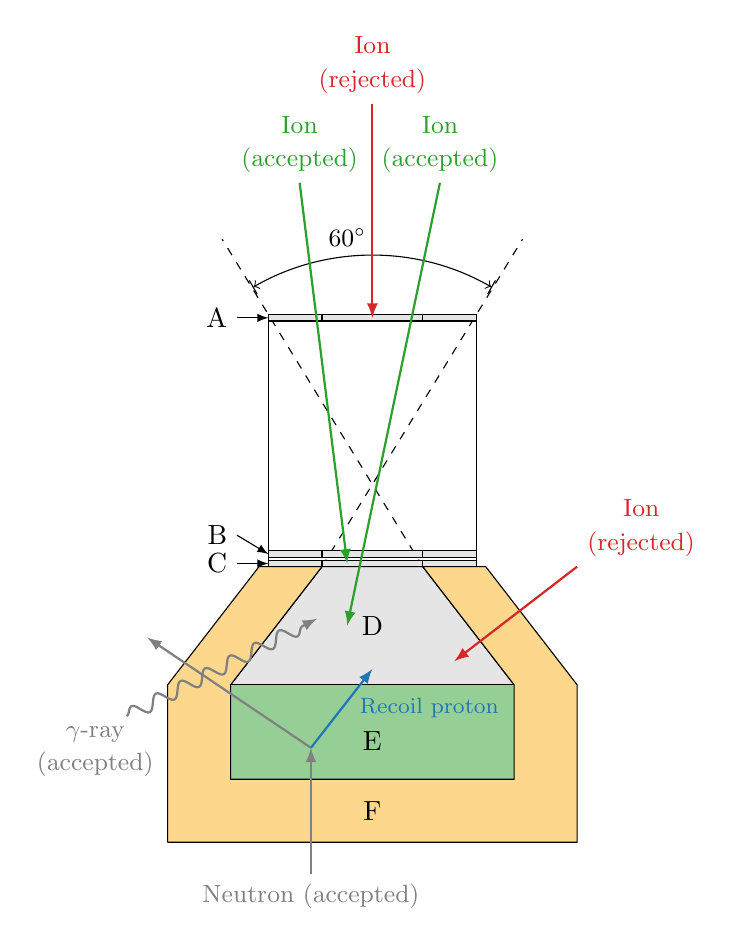
\begin{tikzpicture}[scale=0.8]
    \tikzset{%
        add/.style args={#1 and #2}{
            to path={%
                ($(\tikztostart)!-#1!(\tikztotarget)$)--($(\tikztotarget)!-#2!(\tikztostart)$)%
                \tikztonodes},add/.default={.2 and .2}}
    }  
    
    \def\bottomwidth{3.25}
    \def\midwidth{1.8}
    \def\topwidth{1.65}
    \def\bottomheight{2.5}
    \def\midheight{4.375}
    \def\Fthickness{1}
    \def\Sithickness{0.1}
    \def\BCdistance{0.15}
    \def\topheight{8.375}
    
    % FOV
    \draw[add=0 and 0.3, dashed] (\midwidth - \Fthickness, \midheight) to (-\topwidth, \topheight);
    \draw[add=0 and 0.3, dashed] (-\midwidth + \Fthickness, \midheight) to (\topwidth, \topheight);
    
    \draw[|<->|] (-\topwidth, \topheight) ++ (90+30:0.5) arc (90+30:90-30:{\topheight-\midheight-0.2}) node[pos=0.4, above] {\small\SI{60}{\degree}};

    % A
    \draw[fill=light-gray] (-\topwidth, \topheight - \Sithickness) rectangle (\topwidth, \topheight);
    \draw (-\midwidth + \Fthickness, \topheight - \Sithickness) --  (-\midwidth + \Fthickness, \topheight);
    \draw (-\midwidth + \Fthickness, \topheight - \Sithickness) --  (-\midwidth + \Fthickness, \topheight);
    \draw (\midwidth - \Fthickness, \topheight - \Sithickness) --  (\midwidth - \Fthickness, \topheight);
    \draw (\midwidth - \Fthickness, \topheight - \Sithickness) --  (\midwidth - \Fthickness, \topheight);
    \draw[latex-] (-\topwidth, \topheight - \Sithickness / 2) -- (-\topwidth - 0.5, \topheight - \Sithickness / 2) node[left] {A};
    
    % B
    \draw[fill=light-gray] (-\topwidth, \midheight + \BCdistance) rectangle (\topwidth, \midheight + \BCdistance + \Sithickness);
    \draw (-\midwidth + \Fthickness, \midheight + \BCdistance) --  (-\midwidth + \Fthickness, \midheight + \BCdistance + \Sithickness);
    \draw (-\midwidth + \Fthickness, \midheight + \BCdistance) --  (-\midwidth + \Fthickness, \midheight + \BCdistance + \Sithickness);
    \draw (\midwidth - \Fthickness, \midheight + \BCdistance) --  (\midwidth - \Fthickness, \midheight + \BCdistance + \Sithickness);
    \draw (\midwidth - \Fthickness, \midheight + \BCdistance) --  (\midwidth - \Fthickness, \midheight + \BCdistance + \Sithickness);
    \draw[latex-] (-\topwidth, \midheight + \BCdistance + \Sithickness / 2) -- (-\topwidth - 0.5, \midheight + \BCdistance + \Sithickness / 2 + 0.3) node[left] {B};
    
    % C
    \draw[fill=light-gray] (-\topwidth, \midheight) rectangle (\topwidth, \midheight + \Sithickness);
    \draw (-\midwidth + \Fthickness, \midheight) --  (-\midwidth + \Fthickness, \midheight + \Sithickness);
    \draw (-\midwidth + \Fthickness, \midheight) --  (-\midwidth + \Fthickness, \midheight + \Sithickness);
    \draw (\midwidth - \Fthickness, \midheight) --  (\midwidth - \Fthickness, \midheight + \Sithickness);
    \draw (\midwidth - \Fthickness, \midheight) --  (\midwidth - \Fthickness, \midheight + \Sithickness);
    \draw[latex-] (-\topwidth, \midheight + \Sithickness / 2) -- (-\topwidth - 0.5, \midheight + \Sithickness / 2) node[left] {C};
    
    % border of ABC
    \draw (-\topwidth, \midheight) -- (-\topwidth, \topheight);
    \draw (\topwidth, \midheight) -- (\topwidth, \topheight);
    
    % D
    \draw[fill=light-gray] (\bottomwidth - \Fthickness, \bottomheight) --  (-\bottomwidth + \Fthickness, \bottomheight) -- (-\midwidth + \Fthickness, \midheight) -- (\midwidth - \Fthickness, \midheight) -- (\bottomwidth - \Fthickness, \bottomheight);   
    \node at (0, {\bottomheight + (\midheight - \bottomheight) / 2}) {D};   
    
    % E
    \draw[fill=green!50] (\bottomwidth - \Fthickness, \bottomheight) -- (\bottomwidth - \Fthickness, \Fthickness) --
    (-\bottomwidth + \Fthickness, \Fthickness) --  (-\bottomwidth + \Fthickness, \bottomheight) -- (\bottomwidth - \Fthickness, \bottomheight);  
    \node at (0, {\Fthickness + (\bottomheight - \Fthickness) * 0.4}) {E};   
    
    % F
    \draw[fill=Dandelion!50] (-\bottomwidth, 0) -- (\bottomwidth, 0) -- (\bottomwidth, \bottomheight) -- (\midwidth, \midheight) --
    (\midwidth - \Fthickness, \midheight) -- (\bottomwidth - \Fthickness, \bottomheight) -- (\bottomwidth - \Fthickness, \Fthickness) --
    (-\bottomwidth + \Fthickness, \Fthickness) --  (-\bottomwidth + \Fthickness, \bottomheight) -- (-\midwidth + \Fthickness, \midheight) --
    (-\midwidth, \midheight) -- (-\bottomwidth, \bottomheight) -- (-\bottomwidth, 0);     
    \node at (0, \Fthickness / 2) {F};
    
    % trajectories of ions
    \draw[thick, green, -latex] (-\topwidth*0.7, \topheight*1.25) node[above, align=center] {\small Ion\\ \small (accepted)}
     -- ({-(\midwidth - \Fthickness) * 0.5}, \midheight + \Sithickness / 2);
    \draw[thick, green, -latex] (\topwidth*0.65, \topheight*1.25) node[above, align=center] {\small Ion\\ \small (accepted)}
     -- ({-(\midwidth - \Fthickness) * 0.5}, {\bottomheight +  (\midheight - \bottomheight) / 2});
    \draw[thick, red, -latex] (0, \topheight*1.4) node[above, align=center] {\small Ion\\ \small (rejected)}
     -- (0, \topheight - \Sithickness / 2);
    \draw[thick, red, -latex] (\bottomwidth, \midheight) node[above right, align=center] {\small Ion\\ \small (rejected)}
    -- (\bottomwidth * 0.4, {\bottomheight + (\midheight - \bottomheight) * 0.2});
    
    % trajectory of neutron
    \draw[thick, gray, -latex] (-\bottomwidth*0.3, -0.5) node[below] {\small Neutron (accepted)}
    -- (-\bottomwidth*0.3, {\Fthickness + \bottomheight * 0.2});
    \draw[thick, gray, -latex]  (-\bottomwidth*0.3, {\Fthickness + \bottomheight * 0.2}) -- (-\bottomwidth * 1.1, \bottomheight * 1.3);
    \draw[thick, blue, -latex]  (-\bottomwidth*0.3, {\Fthickness + \bottomheight * 0.2}) -- (0, \bottomheight * 1.1) node[midway, right, xshift=1mm] {\footnotesize Recoil proton};
    
    % trajectory of gamma
    \draw[thick, gray, decorate, decoration=snake] (-\bottomwidth*1.2, \bottomheight * 0.8) node[below, align=center, xshift=-4mm] {\small $\gamma$-ray\\ \small (accepted)} -- (-\bottomwidth * 0.3, \bottomheight * 1.4);
    \draw[thick, gray, -latex] (-\bottomwidth * 0.3, \bottomheight * 1.4) -- ++ (\bottomwidth * 0.03, \bottomheight * 0.02);
    
\end{tikzpicture}
%\end{document}
        \end{column}
    \end{columns}
\end{frame}

\begin{frame}{High Energy Telescope}
    \begin{columns}
    	\begin{column}{0.7\textwidth}
    		\centering
		    %\documentclass{standalone}
%\usepackage[dvipsnames]{xcolor}
%\usepackage{tikz}
%\usepackage{amsmath}
%\usepackage{siunitx}

%\usetikzlibrary{calc}
%\usetikzlibrary{decorations.pathmorphing}

%\definecolor{light-gray}{gray}{0.9}

%\begin{document}
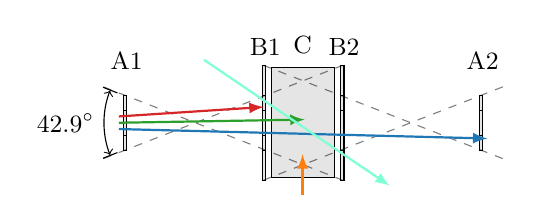
\begin{tikzpicture}[scale=0.4]
    \tikzset{%
        add/.style args={#1 and #2}{
            to path={%
                ($(\tikztostart)!-#1!(\tikztotarget)$)--($(\tikztotarget)!-#2!(\tikztostart)$)%
                \tikztonodes},add/.default={.2 and .2}}
    }   
    
    \def\Sithickness{0.05}
    
    % A1
    \draw[fill=light-gray] (-\Sithickness, -0.87) rectangle (\Sithickness, 0.87) node[above,yshift=2mm]{\small A1};
    \draw (-\Sithickness, -0.4) -- (\Sithickness, -0.4);
    \draw (-\Sithickness, 0.4) -- (\Sithickness, 0.4);
    
    % B1
    \draw[fill=light-gray] (4.4-\Sithickness, -1.82) rectangle (4.4+\Sithickness, 1.82) node[above]{\small B1};
    \draw (4.4-\Sithickness, -0.4) -- (4.4+\Sithickness, -0.4);
    \draw (4.4-\Sithickness, 0.4) -- (4.4+\Sithickness, 0.4);
    \draw (4.4-\Sithickness, -0.87) -- (4.4+\Sithickness, -0.87);
    \draw (4.4-\Sithickness, 0.87) -- (4.4+\Sithickness, 0.87);
    
    % C
    \draw[fill=light-gray] (4.635, -1.75) rectangle ++(2, 3.5);
    \node[above, yshift=0.5mm] at (5.635, 1.75) {\small C};
    
    % B2
    \draw[fill=light-gray] (6.9-\Sithickness, -1.82) rectangle (6.9+\Sithickness, 1.82) node[above]{\small B2};
    \draw (6.9-\Sithickness, -0.4) -- (6.9+\Sithickness, -0.4);
    \draw (6.9-\Sithickness, 0.4) -- (6.9+\Sithickness, 0.4);
    \draw (6.9-\Sithickness, -0.87) -- (6.9+\Sithickness, -0.87);
    \draw (6.9-\Sithickness, 0.87) -- (6.9+\Sithickness, 0.87);
    
    % A2
    \draw[fill=light-gray] (11.3-\Sithickness, -0.87) rectangle (11.3+\Sithickness, 0.87) node[above,yshift=2mm]{\small A2};
    \draw (11.3-\Sithickness, -0.4) -- (11.3+\Sithickness, -0.4);
    \draw (11.3-\Sithickness, 0.4) -- (11.3+\Sithickness, 0.4);
    
    % FOV
    \draw[add=0.1 and 0, dashed, opacity=0.5] (0, -0.87) to (6.9, 1.82);
    \draw[add=0.1 and 0, dashed, opacity=0.5] (0, 0.87) to (6.9, -1.82);
    \draw[add=0.1 and 0, dashed, opacity=0.5] (11.3, -0.87) to (4.4, 1.82);
    \draw[add=0.1 and 0, dashed, opacity=0.5] (11.3, 0.87) to (4.4, -1.82);
    
    \draw[|<->|] (0, 0.87) ++ (180-21.45:0.5) arc (180-21.45:180+21.45:2.4+0.48) node[midway, left] {\small\SI{42.9}{\degree}};
    

    \draw[thick, red, -latex] (-0.2, 0.2) -- (4.4, 0.5);
    \draw[thick, green, -latex] (-0.2, 0) -- (5.7, 0.1);
    \draw[thick, blue, -latex] (-0.2, -0.2) -- (11.5, -0.5);
    \uncover<2->{
        \draw[thick, Aquamarine, -latex] (2.5, 2) -- (8.4, -2);
        \draw[thick, orange, -latex] (5.635, -2.3) -- (5.635, -1);
    }
\end{tikzpicture}
%\end{document}
		\end{column}
		\begin{column}{0.25\textwidth}
			\footnotesize \textcolor{red}{stopping in B}\\ \textcolor{green}{stopping in C} \\ \textcolor{blue}{penetrating}\\ \textcolor{Aquamarine}{GCR channel} \\ \textcolor{orange}{C single counter}
		\end{column}
	\end{columns}
    \begin{columns}
        \begin{column}{0.45\textwidth}
            \begin{itemize}
                \item Part of Solar Orbiter's EPD suite 
                \item Operating since February 2020
                \item Nominal data products: Charged particle spectra above \SI{7}{\mega\electronvolt\per nuc} (ions) and \SI{600}{\kilo\electronvolt} (electrons)
                \item Additional data products with higher statistics suitable for FDs
            \end{itemize}
        \end{column}
        \begin{column}{0.45\textwidth}
            %% Creator: Matplotlib, PGF backend
%%
%% To include the figure in your LaTeX document, write
%%   \input{<filename>.pgf}
%%
%% Make sure the required packages are loaded in your preamble
%%   \usepackage{pgf}
%%
%% and, on pdftex
%%   \usepackage[utf8]{inputenc}\DeclareUnicodeCharacter{2212}{-}
%%
%% or, on luatex and xetex
%%   \usepackage{unicode-math}
%%
%% Figures using additional raster images can only be included by \input if
%% they are in the same directory as the main LaTeX file. For loading figures
%% from other directories you can use the `import` package
%%   \usepackage{import}
%%
%% and then include the figures with
%%   \import{<path to file>}{<filename>.pgf}
%%
%% Matplotlib used the following preamble
%%   \usepackage{siunitx}
%%   \usepackage{fontspec}
%%
\begingroup%
\makeatletter%
\begin{pgfpicture}%
\pgfpathrectangle{\pgfpointorigin}{\pgfqpoint{2.800000in}{1.600000in}}%
\pgfusepath{use as bounding box, clip}%
\begin{pgfscope}%
\pgfsetbuttcap%
\pgfsetmiterjoin%
\definecolor{currentfill}{rgb}{1.000000,1.000000,1.000000}%
\pgfsetfillcolor{currentfill}%
\pgfsetlinewidth{0.000000pt}%
\definecolor{currentstroke}{rgb}{1.000000,1.000000,1.000000}%
\pgfsetstrokecolor{currentstroke}%
\pgfsetdash{}{0pt}%
\pgfpathmoveto{\pgfqpoint{0.000000in}{0.000000in}}%
\pgfpathlineto{\pgfqpoint{2.800000in}{0.000000in}}%
\pgfpathlineto{\pgfqpoint{2.800000in}{1.600000in}}%
\pgfpathlineto{\pgfqpoint{0.000000in}{1.600000in}}%
\pgfpathclose%
\pgfusepath{fill}%
\end{pgfscope}%
\begin{pgfscope}%
\pgfsetbuttcap%
\pgfsetmiterjoin%
\definecolor{currentfill}{rgb}{1.000000,1.000000,1.000000}%
\pgfsetfillcolor{currentfill}%
\pgfsetlinewidth{0.000000pt}%
\definecolor{currentstroke}{rgb}{0.000000,0.000000,0.000000}%
\pgfsetstrokecolor{currentstroke}%
\pgfsetstrokeopacity{0.000000}%
\pgfsetdash{}{0pt}%
\pgfpathmoveto{\pgfqpoint{0.535342in}{0.387868in}}%
\pgfpathlineto{\pgfqpoint{2.692011in}{0.387868in}}%
\pgfpathlineto{\pgfqpoint{2.692011in}{1.461368in}}%
\pgfpathlineto{\pgfqpoint{0.535342in}{1.461368in}}%
\pgfpathclose%
\pgfusepath{fill}%
\end{pgfscope}%
\begin{pgfscope}%
\pgfsetbuttcap%
\pgfsetroundjoin%
\definecolor{currentfill}{rgb}{0.000000,0.000000,0.000000}%
\pgfsetfillcolor{currentfill}%
\pgfsetlinewidth{0.803000pt}%
\definecolor{currentstroke}{rgb}{0.000000,0.000000,0.000000}%
\pgfsetstrokecolor{currentstroke}%
\pgfsetdash{}{0pt}%
\pgfsys@defobject{currentmarker}{\pgfqpoint{0.000000in}{-0.048611in}}{\pgfqpoint{0.000000in}{0.000000in}}{%
\pgfpathmoveto{\pgfqpoint{0.000000in}{0.000000in}}%
\pgfpathlineto{\pgfqpoint{0.000000in}{-0.048611in}}%
\pgfusepath{stroke,fill}%
}%
\begin{pgfscope}%
\pgfsys@transformshift{0.535342in}{0.387868in}%
\pgfsys@useobject{currentmarker}{}%
\end{pgfscope}%
\end{pgfscope}%
\begin{pgfscope}%
\pgfsetbuttcap%
\pgfsetroundjoin%
\definecolor{currentfill}{rgb}{0.000000,0.000000,0.000000}%
\pgfsetfillcolor{currentfill}%
\pgfsetlinewidth{0.803000pt}%
\definecolor{currentstroke}{rgb}{0.000000,0.000000,0.000000}%
\pgfsetstrokecolor{currentstroke}%
\pgfsetdash{}{0pt}%
\pgfsys@defobject{currentmarker}{\pgfqpoint{0.000000in}{-0.048611in}}{\pgfqpoint{0.000000in}{0.000000in}}{%
\pgfpathmoveto{\pgfqpoint{0.000000in}{0.000000in}}%
\pgfpathlineto{\pgfqpoint{0.000000in}{-0.048611in}}%
\pgfusepath{stroke,fill}%
}%
\begin{pgfscope}%
\pgfsys@transformshift{0.543990in}{0.387868in}%
\pgfsys@useobject{currentmarker}{}%
\end{pgfscope}%
\end{pgfscope}%
\begin{pgfscope}%
\definecolor{textcolor}{rgb}{0.000000,0.000000,0.000000}%
\pgfsetstrokecolor{textcolor}%
\pgfsetfillcolor{textcolor}%
\pgftext[x=0.543990in,y=0.290646in,,top]{\color{textcolor}\sffamily\fontsize{7.000000}{8.400000}\selectfont Mar}%
\end{pgfscope}%
\begin{pgfscope}%
\pgfsetbuttcap%
\pgfsetroundjoin%
\definecolor{currentfill}{rgb}{0.000000,0.000000,0.000000}%
\pgfsetfillcolor{currentfill}%
\pgfsetlinewidth{0.803000pt}%
\definecolor{currentstroke}{rgb}{0.000000,0.000000,0.000000}%
\pgfsetstrokecolor{currentstroke}%
\pgfsetdash{}{0pt}%
\pgfsys@defobject{currentmarker}{\pgfqpoint{0.000000in}{-0.048611in}}{\pgfqpoint{0.000000in}{0.000000in}}{%
\pgfpathmoveto{\pgfqpoint{0.000000in}{0.000000in}}%
\pgfpathlineto{\pgfqpoint{0.000000in}{-0.048611in}}%
\pgfusepath{stroke,fill}%
}%
\begin{pgfscope}%
\pgfsys@transformshift{0.751539in}{0.387868in}%
\pgfsys@useobject{currentmarker}{}%
\end{pgfscope}%
\end{pgfscope}%
\begin{pgfscope}%
\definecolor{textcolor}{rgb}{0.000000,0.000000,0.000000}%
\pgfsetstrokecolor{textcolor}%
\pgfsetfillcolor{textcolor}%
\pgftext[x=0.751539in,y=0.290646in,,top]{\color{textcolor}\sffamily\fontsize{7.000000}{8.400000}\selectfont Apr}%
\end{pgfscope}%
\begin{pgfscope}%
\pgfsetbuttcap%
\pgfsetroundjoin%
\definecolor{currentfill}{rgb}{0.000000,0.000000,0.000000}%
\pgfsetfillcolor{currentfill}%
\pgfsetlinewidth{0.803000pt}%
\definecolor{currentstroke}{rgb}{0.000000,0.000000,0.000000}%
\pgfsetstrokecolor{currentstroke}%
\pgfsetdash{}{0pt}%
\pgfsys@defobject{currentmarker}{\pgfqpoint{0.000000in}{-0.048611in}}{\pgfqpoint{0.000000in}{0.000000in}}{%
\pgfpathmoveto{\pgfqpoint{0.000000in}{0.000000in}}%
\pgfpathlineto{\pgfqpoint{0.000000in}{-0.048611in}}%
\pgfusepath{stroke,fill}%
}%
\begin{pgfscope}%
\pgfsys@transformshift{0.952393in}{0.387868in}%
\pgfsys@useobject{currentmarker}{}%
\end{pgfscope}%
\end{pgfscope}%
\begin{pgfscope}%
\definecolor{textcolor}{rgb}{0.000000,0.000000,0.000000}%
\pgfsetstrokecolor{textcolor}%
\pgfsetfillcolor{textcolor}%
\pgftext[x=0.952393in,y=0.290646in,,top]{\color{textcolor}\sffamily\fontsize{7.000000}{8.400000}\selectfont May}%
\end{pgfscope}%
\begin{pgfscope}%
\pgfsetbuttcap%
\pgfsetroundjoin%
\definecolor{currentfill}{rgb}{0.000000,0.000000,0.000000}%
\pgfsetfillcolor{currentfill}%
\pgfsetlinewidth{0.803000pt}%
\definecolor{currentstroke}{rgb}{0.000000,0.000000,0.000000}%
\pgfsetstrokecolor{currentstroke}%
\pgfsetdash{}{0pt}%
\pgfsys@defobject{currentmarker}{\pgfqpoint{0.000000in}{-0.048611in}}{\pgfqpoint{0.000000in}{0.000000in}}{%
\pgfpathmoveto{\pgfqpoint{0.000000in}{0.000000in}}%
\pgfpathlineto{\pgfqpoint{0.000000in}{-0.048611in}}%
\pgfusepath{stroke,fill}%
}%
\begin{pgfscope}%
\pgfsys@transformshift{1.159942in}{0.387868in}%
\pgfsys@useobject{currentmarker}{}%
\end{pgfscope}%
\end{pgfscope}%
\begin{pgfscope}%
\definecolor{textcolor}{rgb}{0.000000,0.000000,0.000000}%
\pgfsetstrokecolor{textcolor}%
\pgfsetfillcolor{textcolor}%
\pgftext[x=1.159942in,y=0.290646in,,top]{\color{textcolor}\sffamily\fontsize{7.000000}{8.400000}\selectfont Jun}%
\end{pgfscope}%
\begin{pgfscope}%
\pgfsetbuttcap%
\pgfsetroundjoin%
\definecolor{currentfill}{rgb}{0.000000,0.000000,0.000000}%
\pgfsetfillcolor{currentfill}%
\pgfsetlinewidth{0.803000pt}%
\definecolor{currentstroke}{rgb}{0.000000,0.000000,0.000000}%
\pgfsetstrokecolor{currentstroke}%
\pgfsetdash{}{0pt}%
\pgfsys@defobject{currentmarker}{\pgfqpoint{0.000000in}{-0.048611in}}{\pgfqpoint{0.000000in}{0.000000in}}{%
\pgfpathmoveto{\pgfqpoint{0.000000in}{0.000000in}}%
\pgfpathlineto{\pgfqpoint{0.000000in}{-0.048611in}}%
\pgfusepath{stroke,fill}%
}%
\begin{pgfscope}%
\pgfsys@transformshift{1.360796in}{0.387868in}%
\pgfsys@useobject{currentmarker}{}%
\end{pgfscope}%
\end{pgfscope}%
\begin{pgfscope}%
\definecolor{textcolor}{rgb}{0.000000,0.000000,0.000000}%
\pgfsetstrokecolor{textcolor}%
\pgfsetfillcolor{textcolor}%
\pgftext[x=1.360796in,y=0.290646in,,top]{\color{textcolor}\sffamily\fontsize{7.000000}{8.400000}\selectfont Jul}%
\end{pgfscope}%
\begin{pgfscope}%
\pgfsetbuttcap%
\pgfsetroundjoin%
\definecolor{currentfill}{rgb}{0.000000,0.000000,0.000000}%
\pgfsetfillcolor{currentfill}%
\pgfsetlinewidth{0.803000pt}%
\definecolor{currentstroke}{rgb}{0.000000,0.000000,0.000000}%
\pgfsetstrokecolor{currentstroke}%
\pgfsetdash{}{0pt}%
\pgfsys@defobject{currentmarker}{\pgfqpoint{0.000000in}{-0.048611in}}{\pgfqpoint{0.000000in}{0.000000in}}{%
\pgfpathmoveto{\pgfqpoint{0.000000in}{0.000000in}}%
\pgfpathlineto{\pgfqpoint{0.000000in}{-0.048611in}}%
\pgfusepath{stroke,fill}%
}%
\begin{pgfscope}%
\pgfsys@transformshift{1.568345in}{0.387868in}%
\pgfsys@useobject{currentmarker}{}%
\end{pgfscope}%
\end{pgfscope}%
\begin{pgfscope}%
\definecolor{textcolor}{rgb}{0.000000,0.000000,0.000000}%
\pgfsetstrokecolor{textcolor}%
\pgfsetfillcolor{textcolor}%
\pgftext[x=1.568345in,y=0.290646in,,top]{\color{textcolor}\sffamily\fontsize{7.000000}{8.400000}\selectfont Aug}%
\end{pgfscope}%
\begin{pgfscope}%
\pgfsetbuttcap%
\pgfsetroundjoin%
\definecolor{currentfill}{rgb}{0.000000,0.000000,0.000000}%
\pgfsetfillcolor{currentfill}%
\pgfsetlinewidth{0.803000pt}%
\definecolor{currentstroke}{rgb}{0.000000,0.000000,0.000000}%
\pgfsetstrokecolor{currentstroke}%
\pgfsetdash{}{0pt}%
\pgfsys@defobject{currentmarker}{\pgfqpoint{0.000000in}{-0.048611in}}{\pgfqpoint{0.000000in}{0.000000in}}{%
\pgfpathmoveto{\pgfqpoint{0.000000in}{0.000000in}}%
\pgfpathlineto{\pgfqpoint{0.000000in}{-0.048611in}}%
\pgfusepath{stroke,fill}%
}%
\begin{pgfscope}%
\pgfsys@transformshift{1.775894in}{0.387868in}%
\pgfsys@useobject{currentmarker}{}%
\end{pgfscope}%
\end{pgfscope}%
\begin{pgfscope}%
\definecolor{textcolor}{rgb}{0.000000,0.000000,0.000000}%
\pgfsetstrokecolor{textcolor}%
\pgfsetfillcolor{textcolor}%
\pgftext[x=1.775894in,y=0.290646in,,top]{\color{textcolor}\sffamily\fontsize{7.000000}{8.400000}\selectfont Sep}%
\end{pgfscope}%
\begin{pgfscope}%
\pgfsetbuttcap%
\pgfsetroundjoin%
\definecolor{currentfill}{rgb}{0.000000,0.000000,0.000000}%
\pgfsetfillcolor{currentfill}%
\pgfsetlinewidth{0.803000pt}%
\definecolor{currentstroke}{rgb}{0.000000,0.000000,0.000000}%
\pgfsetstrokecolor{currentstroke}%
\pgfsetdash{}{0pt}%
\pgfsys@defobject{currentmarker}{\pgfqpoint{0.000000in}{-0.048611in}}{\pgfqpoint{0.000000in}{0.000000in}}{%
\pgfpathmoveto{\pgfqpoint{0.000000in}{0.000000in}}%
\pgfpathlineto{\pgfqpoint{0.000000in}{-0.048611in}}%
\pgfusepath{stroke,fill}%
}%
\begin{pgfscope}%
\pgfsys@transformshift{1.976748in}{0.387868in}%
\pgfsys@useobject{currentmarker}{}%
\end{pgfscope}%
\end{pgfscope}%
\begin{pgfscope}%
\definecolor{textcolor}{rgb}{0.000000,0.000000,0.000000}%
\pgfsetstrokecolor{textcolor}%
\pgfsetfillcolor{textcolor}%
\pgftext[x=1.976748in,y=0.290646in,,top]{\color{textcolor}\sffamily\fontsize{7.000000}{8.400000}\selectfont Oct}%
\end{pgfscope}%
\begin{pgfscope}%
\pgfsetbuttcap%
\pgfsetroundjoin%
\definecolor{currentfill}{rgb}{0.000000,0.000000,0.000000}%
\pgfsetfillcolor{currentfill}%
\pgfsetlinewidth{0.803000pt}%
\definecolor{currentstroke}{rgb}{0.000000,0.000000,0.000000}%
\pgfsetstrokecolor{currentstroke}%
\pgfsetdash{}{0pt}%
\pgfsys@defobject{currentmarker}{\pgfqpoint{0.000000in}{-0.048611in}}{\pgfqpoint{0.000000in}{0.000000in}}{%
\pgfpathmoveto{\pgfqpoint{0.000000in}{0.000000in}}%
\pgfpathlineto{\pgfqpoint{0.000000in}{-0.048611in}}%
\pgfusepath{stroke,fill}%
}%
\begin{pgfscope}%
\pgfsys@transformshift{2.184297in}{0.387868in}%
\pgfsys@useobject{currentmarker}{}%
\end{pgfscope}%
\end{pgfscope}%
\begin{pgfscope}%
\definecolor{textcolor}{rgb}{0.000000,0.000000,0.000000}%
\pgfsetstrokecolor{textcolor}%
\pgfsetfillcolor{textcolor}%
\pgftext[x=2.184297in,y=0.290646in,,top]{\color{textcolor}\sffamily\fontsize{7.000000}{8.400000}\selectfont Nov}%
\end{pgfscope}%
\begin{pgfscope}%
\pgfsetbuttcap%
\pgfsetroundjoin%
\definecolor{currentfill}{rgb}{0.000000,0.000000,0.000000}%
\pgfsetfillcolor{currentfill}%
\pgfsetlinewidth{0.803000pt}%
\definecolor{currentstroke}{rgb}{0.000000,0.000000,0.000000}%
\pgfsetstrokecolor{currentstroke}%
\pgfsetdash{}{0pt}%
\pgfsys@defobject{currentmarker}{\pgfqpoint{0.000000in}{-0.048611in}}{\pgfqpoint{0.000000in}{0.000000in}}{%
\pgfpathmoveto{\pgfqpoint{0.000000in}{0.000000in}}%
\pgfpathlineto{\pgfqpoint{0.000000in}{-0.048611in}}%
\pgfusepath{stroke,fill}%
}%
\begin{pgfscope}%
\pgfsys@transformshift{2.385151in}{0.387868in}%
\pgfsys@useobject{currentmarker}{}%
\end{pgfscope}%
\end{pgfscope}%
\begin{pgfscope}%
\definecolor{textcolor}{rgb}{0.000000,0.000000,0.000000}%
\pgfsetstrokecolor{textcolor}%
\pgfsetfillcolor{textcolor}%
\pgftext[x=2.385151in,y=0.290646in,,top]{\color{textcolor}\sffamily\fontsize{7.000000}{8.400000}\selectfont Dec}%
\end{pgfscope}%
\begin{pgfscope}%
\pgfsetbuttcap%
\pgfsetroundjoin%
\definecolor{currentfill}{rgb}{0.000000,0.000000,0.000000}%
\pgfsetfillcolor{currentfill}%
\pgfsetlinewidth{0.803000pt}%
\definecolor{currentstroke}{rgb}{0.000000,0.000000,0.000000}%
\pgfsetstrokecolor{currentstroke}%
\pgfsetdash{}{0pt}%
\pgfsys@defobject{currentmarker}{\pgfqpoint{0.000000in}{-0.048611in}}{\pgfqpoint{0.000000in}{0.000000in}}{%
\pgfpathmoveto{\pgfqpoint{0.000000in}{0.000000in}}%
\pgfpathlineto{\pgfqpoint{0.000000in}{-0.048611in}}%
\pgfusepath{stroke,fill}%
}%
\begin{pgfscope}%
\pgfsys@transformshift{2.592700in}{0.387868in}%
\pgfsys@useobject{currentmarker}{}%
\end{pgfscope}%
\end{pgfscope}%
\begin{pgfscope}%
\definecolor{textcolor}{rgb}{0.000000,0.000000,0.000000}%
\pgfsetstrokecolor{textcolor}%
\pgfsetfillcolor{textcolor}%
\pgftext[x=2.516818in, y=0.223174in, left, base]{\color{textcolor}\sffamily\fontsize{7.000000}{8.400000}\selectfont Jan}%
\end{pgfscope}%
\begin{pgfscope}%
\definecolor{textcolor}{rgb}{0.000000,0.000000,0.000000}%
\pgfsetstrokecolor{textcolor}%
\pgfsetfillcolor{textcolor}%
\pgftext[x=2.489450in, y=0.123346in, left, base]{\color{textcolor}\sffamily\fontsize{7.000000}{8.400000}\selectfont 2021}%
\end{pgfscope}%
\begin{pgfscope}%
\pgfsetbuttcap%
\pgfsetroundjoin%
\definecolor{currentfill}{rgb}{0.000000,0.000000,0.000000}%
\pgfsetfillcolor{currentfill}%
\pgfsetlinewidth{0.803000pt}%
\definecolor{currentstroke}{rgb}{0.000000,0.000000,0.000000}%
\pgfsetstrokecolor{currentstroke}%
\pgfsetdash{}{0pt}%
\pgfsys@defobject{currentmarker}{\pgfqpoint{0.000000in}{-0.048611in}}{\pgfqpoint{0.000000in}{0.000000in}}{%
\pgfpathmoveto{\pgfqpoint{0.000000in}{0.000000in}}%
\pgfpathlineto{\pgfqpoint{0.000000in}{-0.048611in}}%
\pgfusepath{stroke,fill}%
}%
\begin{pgfscope}%
\pgfsys@transformshift{2.692011in}{0.387868in}%
\pgfsys@useobject{currentmarker}{}%
\end{pgfscope}%
\end{pgfscope}%
\begin{pgfscope}%
\pgfsetbuttcap%
\pgfsetroundjoin%
\definecolor{currentfill}{rgb}{0.000000,0.000000,0.000000}%
\pgfsetfillcolor{currentfill}%
\pgfsetlinewidth{0.602250pt}%
\definecolor{currentstroke}{rgb}{0.000000,0.000000,0.000000}%
\pgfsetstrokecolor{currentstroke}%
\pgfsetdash{}{0pt}%
\pgfsys@defobject{currentmarker}{\pgfqpoint{0.000000in}{-0.027778in}}{\pgfqpoint{0.000000in}{0.000000in}}{%
\pgfpathmoveto{\pgfqpoint{0.000000in}{0.000000in}}%
\pgfpathlineto{\pgfqpoint{0.000000in}{-0.027778in}}%
\pgfusepath{stroke,fill}%
}%
\begin{pgfscope}%
\pgfsys@transformshift{0.550685in}{0.387868in}%
\pgfsys@useobject{currentmarker}{}%
\end{pgfscope}%
\end{pgfscope}%
\begin{pgfscope}%
\pgfsetbuttcap%
\pgfsetroundjoin%
\definecolor{currentfill}{rgb}{0.000000,0.000000,0.000000}%
\pgfsetfillcolor{currentfill}%
\pgfsetlinewidth{0.602250pt}%
\definecolor{currentstroke}{rgb}{0.000000,0.000000,0.000000}%
\pgfsetstrokecolor{currentstroke}%
\pgfsetdash{}{0pt}%
\pgfsys@defobject{currentmarker}{\pgfqpoint{0.000000in}{-0.027778in}}{\pgfqpoint{0.000000in}{0.000000in}}{%
\pgfpathmoveto{\pgfqpoint{0.000000in}{0.000000in}}%
\pgfpathlineto{\pgfqpoint{0.000000in}{-0.027778in}}%
\pgfusepath{stroke,fill}%
}%
\begin{pgfscope}%
\pgfsys@transformshift{0.597551in}{0.387868in}%
\pgfsys@useobject{currentmarker}{}%
\end{pgfscope}%
\end{pgfscope}%
\begin{pgfscope}%
\pgfsetbuttcap%
\pgfsetroundjoin%
\definecolor{currentfill}{rgb}{0.000000,0.000000,0.000000}%
\pgfsetfillcolor{currentfill}%
\pgfsetlinewidth{0.602250pt}%
\definecolor{currentstroke}{rgb}{0.000000,0.000000,0.000000}%
\pgfsetstrokecolor{currentstroke}%
\pgfsetdash{}{0pt}%
\pgfsys@defobject{currentmarker}{\pgfqpoint{0.000000in}{-0.027778in}}{\pgfqpoint{0.000000in}{0.000000in}}{%
\pgfpathmoveto{\pgfqpoint{0.000000in}{0.000000in}}%
\pgfpathlineto{\pgfqpoint{0.000000in}{-0.027778in}}%
\pgfusepath{stroke,fill}%
}%
\begin{pgfscope}%
\pgfsys@transformshift{0.644416in}{0.387868in}%
\pgfsys@useobject{currentmarker}{}%
\end{pgfscope}%
\end{pgfscope}%
\begin{pgfscope}%
\pgfsetbuttcap%
\pgfsetroundjoin%
\definecolor{currentfill}{rgb}{0.000000,0.000000,0.000000}%
\pgfsetfillcolor{currentfill}%
\pgfsetlinewidth{0.602250pt}%
\definecolor{currentstroke}{rgb}{0.000000,0.000000,0.000000}%
\pgfsetstrokecolor{currentstroke}%
\pgfsetdash{}{0pt}%
\pgfsys@defobject{currentmarker}{\pgfqpoint{0.000000in}{-0.027778in}}{\pgfqpoint{0.000000in}{0.000000in}}{%
\pgfpathmoveto{\pgfqpoint{0.000000in}{0.000000in}}%
\pgfpathlineto{\pgfqpoint{0.000000in}{-0.027778in}}%
\pgfusepath{stroke,fill}%
}%
\begin{pgfscope}%
\pgfsys@transformshift{0.691282in}{0.387868in}%
\pgfsys@useobject{currentmarker}{}%
\end{pgfscope}%
\end{pgfscope}%
\begin{pgfscope}%
\pgfsetbuttcap%
\pgfsetroundjoin%
\definecolor{currentfill}{rgb}{0.000000,0.000000,0.000000}%
\pgfsetfillcolor{currentfill}%
\pgfsetlinewidth{0.602250pt}%
\definecolor{currentstroke}{rgb}{0.000000,0.000000,0.000000}%
\pgfsetstrokecolor{currentstroke}%
\pgfsetdash{}{0pt}%
\pgfsys@defobject{currentmarker}{\pgfqpoint{0.000000in}{-0.027778in}}{\pgfqpoint{0.000000in}{0.000000in}}{%
\pgfpathmoveto{\pgfqpoint{0.000000in}{0.000000in}}%
\pgfpathlineto{\pgfqpoint{0.000000in}{-0.027778in}}%
\pgfusepath{stroke,fill}%
}%
\begin{pgfscope}%
\pgfsys@transformshift{0.738148in}{0.387868in}%
\pgfsys@useobject{currentmarker}{}%
\end{pgfscope}%
\end{pgfscope}%
\begin{pgfscope}%
\pgfsetbuttcap%
\pgfsetroundjoin%
\definecolor{currentfill}{rgb}{0.000000,0.000000,0.000000}%
\pgfsetfillcolor{currentfill}%
\pgfsetlinewidth{0.602250pt}%
\definecolor{currentstroke}{rgb}{0.000000,0.000000,0.000000}%
\pgfsetstrokecolor{currentstroke}%
\pgfsetdash{}{0pt}%
\pgfsys@defobject{currentmarker}{\pgfqpoint{0.000000in}{-0.027778in}}{\pgfqpoint{0.000000in}{0.000000in}}{%
\pgfpathmoveto{\pgfqpoint{0.000000in}{0.000000in}}%
\pgfpathlineto{\pgfqpoint{0.000000in}{-0.027778in}}%
\pgfusepath{stroke,fill}%
}%
\begin{pgfscope}%
\pgfsys@transformshift{0.785014in}{0.387868in}%
\pgfsys@useobject{currentmarker}{}%
\end{pgfscope}%
\end{pgfscope}%
\begin{pgfscope}%
\pgfsetbuttcap%
\pgfsetroundjoin%
\definecolor{currentfill}{rgb}{0.000000,0.000000,0.000000}%
\pgfsetfillcolor{currentfill}%
\pgfsetlinewidth{0.602250pt}%
\definecolor{currentstroke}{rgb}{0.000000,0.000000,0.000000}%
\pgfsetstrokecolor{currentstroke}%
\pgfsetdash{}{0pt}%
\pgfsys@defobject{currentmarker}{\pgfqpoint{0.000000in}{-0.027778in}}{\pgfqpoint{0.000000in}{0.000000in}}{%
\pgfpathmoveto{\pgfqpoint{0.000000in}{0.000000in}}%
\pgfpathlineto{\pgfqpoint{0.000000in}{-0.027778in}}%
\pgfusepath{stroke,fill}%
}%
\begin{pgfscope}%
\pgfsys@transformshift{0.831880in}{0.387868in}%
\pgfsys@useobject{currentmarker}{}%
\end{pgfscope}%
\end{pgfscope}%
\begin{pgfscope}%
\pgfsetbuttcap%
\pgfsetroundjoin%
\definecolor{currentfill}{rgb}{0.000000,0.000000,0.000000}%
\pgfsetfillcolor{currentfill}%
\pgfsetlinewidth{0.602250pt}%
\definecolor{currentstroke}{rgb}{0.000000,0.000000,0.000000}%
\pgfsetstrokecolor{currentstroke}%
\pgfsetdash{}{0pt}%
\pgfsys@defobject{currentmarker}{\pgfqpoint{0.000000in}{-0.027778in}}{\pgfqpoint{0.000000in}{0.000000in}}{%
\pgfpathmoveto{\pgfqpoint{0.000000in}{0.000000in}}%
\pgfpathlineto{\pgfqpoint{0.000000in}{-0.027778in}}%
\pgfusepath{stroke,fill}%
}%
\begin{pgfscope}%
\pgfsys@transformshift{0.878746in}{0.387868in}%
\pgfsys@useobject{currentmarker}{}%
\end{pgfscope}%
\end{pgfscope}%
\begin{pgfscope}%
\pgfsetbuttcap%
\pgfsetroundjoin%
\definecolor{currentfill}{rgb}{0.000000,0.000000,0.000000}%
\pgfsetfillcolor{currentfill}%
\pgfsetlinewidth{0.602250pt}%
\definecolor{currentstroke}{rgb}{0.000000,0.000000,0.000000}%
\pgfsetstrokecolor{currentstroke}%
\pgfsetdash{}{0pt}%
\pgfsys@defobject{currentmarker}{\pgfqpoint{0.000000in}{-0.027778in}}{\pgfqpoint{0.000000in}{0.000000in}}{%
\pgfpathmoveto{\pgfqpoint{0.000000in}{0.000000in}}%
\pgfpathlineto{\pgfqpoint{0.000000in}{-0.027778in}}%
\pgfusepath{stroke,fill}%
}%
\begin{pgfscope}%
\pgfsys@transformshift{0.925612in}{0.387868in}%
\pgfsys@useobject{currentmarker}{}%
\end{pgfscope}%
\end{pgfscope}%
\begin{pgfscope}%
\pgfsetbuttcap%
\pgfsetroundjoin%
\definecolor{currentfill}{rgb}{0.000000,0.000000,0.000000}%
\pgfsetfillcolor{currentfill}%
\pgfsetlinewidth{0.602250pt}%
\definecolor{currentstroke}{rgb}{0.000000,0.000000,0.000000}%
\pgfsetstrokecolor{currentstroke}%
\pgfsetdash{}{0pt}%
\pgfsys@defobject{currentmarker}{\pgfqpoint{0.000000in}{-0.027778in}}{\pgfqpoint{0.000000in}{0.000000in}}{%
\pgfpathmoveto{\pgfqpoint{0.000000in}{0.000000in}}%
\pgfpathlineto{\pgfqpoint{0.000000in}{-0.027778in}}%
\pgfusepath{stroke,fill}%
}%
\begin{pgfscope}%
\pgfsys@transformshift{0.972478in}{0.387868in}%
\pgfsys@useobject{currentmarker}{}%
\end{pgfscope}%
\end{pgfscope}%
\begin{pgfscope}%
\pgfsetbuttcap%
\pgfsetroundjoin%
\definecolor{currentfill}{rgb}{0.000000,0.000000,0.000000}%
\pgfsetfillcolor{currentfill}%
\pgfsetlinewidth{0.602250pt}%
\definecolor{currentstroke}{rgb}{0.000000,0.000000,0.000000}%
\pgfsetstrokecolor{currentstroke}%
\pgfsetdash{}{0pt}%
\pgfsys@defobject{currentmarker}{\pgfqpoint{0.000000in}{-0.027778in}}{\pgfqpoint{0.000000in}{0.000000in}}{%
\pgfpathmoveto{\pgfqpoint{0.000000in}{0.000000in}}%
\pgfpathlineto{\pgfqpoint{0.000000in}{-0.027778in}}%
\pgfusepath{stroke,fill}%
}%
\begin{pgfscope}%
\pgfsys@transformshift{1.019344in}{0.387868in}%
\pgfsys@useobject{currentmarker}{}%
\end{pgfscope}%
\end{pgfscope}%
\begin{pgfscope}%
\pgfsetbuttcap%
\pgfsetroundjoin%
\definecolor{currentfill}{rgb}{0.000000,0.000000,0.000000}%
\pgfsetfillcolor{currentfill}%
\pgfsetlinewidth{0.602250pt}%
\definecolor{currentstroke}{rgb}{0.000000,0.000000,0.000000}%
\pgfsetstrokecolor{currentstroke}%
\pgfsetdash{}{0pt}%
\pgfsys@defobject{currentmarker}{\pgfqpoint{0.000000in}{-0.027778in}}{\pgfqpoint{0.000000in}{0.000000in}}{%
\pgfpathmoveto{\pgfqpoint{0.000000in}{0.000000in}}%
\pgfpathlineto{\pgfqpoint{0.000000in}{-0.027778in}}%
\pgfusepath{stroke,fill}%
}%
\begin{pgfscope}%
\pgfsys@transformshift{1.066210in}{0.387868in}%
\pgfsys@useobject{currentmarker}{}%
\end{pgfscope}%
\end{pgfscope}%
\begin{pgfscope}%
\pgfsetbuttcap%
\pgfsetroundjoin%
\definecolor{currentfill}{rgb}{0.000000,0.000000,0.000000}%
\pgfsetfillcolor{currentfill}%
\pgfsetlinewidth{0.602250pt}%
\definecolor{currentstroke}{rgb}{0.000000,0.000000,0.000000}%
\pgfsetstrokecolor{currentstroke}%
\pgfsetdash{}{0pt}%
\pgfsys@defobject{currentmarker}{\pgfqpoint{0.000000in}{-0.027778in}}{\pgfqpoint{0.000000in}{0.000000in}}{%
\pgfpathmoveto{\pgfqpoint{0.000000in}{0.000000in}}%
\pgfpathlineto{\pgfqpoint{0.000000in}{-0.027778in}}%
\pgfusepath{stroke,fill}%
}%
\begin{pgfscope}%
\pgfsys@transformshift{1.113076in}{0.387868in}%
\pgfsys@useobject{currentmarker}{}%
\end{pgfscope}%
\end{pgfscope}%
\begin{pgfscope}%
\pgfsetbuttcap%
\pgfsetroundjoin%
\definecolor{currentfill}{rgb}{0.000000,0.000000,0.000000}%
\pgfsetfillcolor{currentfill}%
\pgfsetlinewidth{0.602250pt}%
\definecolor{currentstroke}{rgb}{0.000000,0.000000,0.000000}%
\pgfsetstrokecolor{currentstroke}%
\pgfsetdash{}{0pt}%
\pgfsys@defobject{currentmarker}{\pgfqpoint{0.000000in}{-0.027778in}}{\pgfqpoint{0.000000in}{0.000000in}}{%
\pgfpathmoveto{\pgfqpoint{0.000000in}{0.000000in}}%
\pgfpathlineto{\pgfqpoint{0.000000in}{-0.027778in}}%
\pgfusepath{stroke,fill}%
}%
\begin{pgfscope}%
\pgfsys@transformshift{1.206808in}{0.387868in}%
\pgfsys@useobject{currentmarker}{}%
\end{pgfscope}%
\end{pgfscope}%
\begin{pgfscope}%
\pgfsetbuttcap%
\pgfsetroundjoin%
\definecolor{currentfill}{rgb}{0.000000,0.000000,0.000000}%
\pgfsetfillcolor{currentfill}%
\pgfsetlinewidth{0.602250pt}%
\definecolor{currentstroke}{rgb}{0.000000,0.000000,0.000000}%
\pgfsetstrokecolor{currentstroke}%
\pgfsetdash{}{0pt}%
\pgfsys@defobject{currentmarker}{\pgfqpoint{0.000000in}{-0.027778in}}{\pgfqpoint{0.000000in}{0.000000in}}{%
\pgfpathmoveto{\pgfqpoint{0.000000in}{0.000000in}}%
\pgfpathlineto{\pgfqpoint{0.000000in}{-0.027778in}}%
\pgfusepath{stroke,fill}%
}%
\begin{pgfscope}%
\pgfsys@transformshift{1.253674in}{0.387868in}%
\pgfsys@useobject{currentmarker}{}%
\end{pgfscope}%
\end{pgfscope}%
\begin{pgfscope}%
\pgfsetbuttcap%
\pgfsetroundjoin%
\definecolor{currentfill}{rgb}{0.000000,0.000000,0.000000}%
\pgfsetfillcolor{currentfill}%
\pgfsetlinewidth{0.602250pt}%
\definecolor{currentstroke}{rgb}{0.000000,0.000000,0.000000}%
\pgfsetstrokecolor{currentstroke}%
\pgfsetdash{}{0pt}%
\pgfsys@defobject{currentmarker}{\pgfqpoint{0.000000in}{-0.027778in}}{\pgfqpoint{0.000000in}{0.000000in}}{%
\pgfpathmoveto{\pgfqpoint{0.000000in}{0.000000in}}%
\pgfpathlineto{\pgfqpoint{0.000000in}{-0.027778in}}%
\pgfusepath{stroke,fill}%
}%
\begin{pgfscope}%
\pgfsys@transformshift{1.300539in}{0.387868in}%
\pgfsys@useobject{currentmarker}{}%
\end{pgfscope}%
\end{pgfscope}%
\begin{pgfscope}%
\pgfsetbuttcap%
\pgfsetroundjoin%
\definecolor{currentfill}{rgb}{0.000000,0.000000,0.000000}%
\pgfsetfillcolor{currentfill}%
\pgfsetlinewidth{0.602250pt}%
\definecolor{currentstroke}{rgb}{0.000000,0.000000,0.000000}%
\pgfsetstrokecolor{currentstroke}%
\pgfsetdash{}{0pt}%
\pgfsys@defobject{currentmarker}{\pgfqpoint{0.000000in}{-0.027778in}}{\pgfqpoint{0.000000in}{0.000000in}}{%
\pgfpathmoveto{\pgfqpoint{0.000000in}{0.000000in}}%
\pgfpathlineto{\pgfqpoint{0.000000in}{-0.027778in}}%
\pgfusepath{stroke,fill}%
}%
\begin{pgfscope}%
\pgfsys@transformshift{1.347405in}{0.387868in}%
\pgfsys@useobject{currentmarker}{}%
\end{pgfscope}%
\end{pgfscope}%
\begin{pgfscope}%
\pgfsetbuttcap%
\pgfsetroundjoin%
\definecolor{currentfill}{rgb}{0.000000,0.000000,0.000000}%
\pgfsetfillcolor{currentfill}%
\pgfsetlinewidth{0.602250pt}%
\definecolor{currentstroke}{rgb}{0.000000,0.000000,0.000000}%
\pgfsetstrokecolor{currentstroke}%
\pgfsetdash{}{0pt}%
\pgfsys@defobject{currentmarker}{\pgfqpoint{0.000000in}{-0.027778in}}{\pgfqpoint{0.000000in}{0.000000in}}{%
\pgfpathmoveto{\pgfqpoint{0.000000in}{0.000000in}}%
\pgfpathlineto{\pgfqpoint{0.000000in}{-0.027778in}}%
\pgfusepath{stroke,fill}%
}%
\begin{pgfscope}%
\pgfsys@transformshift{1.394271in}{0.387868in}%
\pgfsys@useobject{currentmarker}{}%
\end{pgfscope}%
\end{pgfscope}%
\begin{pgfscope}%
\pgfsetbuttcap%
\pgfsetroundjoin%
\definecolor{currentfill}{rgb}{0.000000,0.000000,0.000000}%
\pgfsetfillcolor{currentfill}%
\pgfsetlinewidth{0.602250pt}%
\definecolor{currentstroke}{rgb}{0.000000,0.000000,0.000000}%
\pgfsetstrokecolor{currentstroke}%
\pgfsetdash{}{0pt}%
\pgfsys@defobject{currentmarker}{\pgfqpoint{0.000000in}{-0.027778in}}{\pgfqpoint{0.000000in}{0.000000in}}{%
\pgfpathmoveto{\pgfqpoint{0.000000in}{0.000000in}}%
\pgfpathlineto{\pgfqpoint{0.000000in}{-0.027778in}}%
\pgfusepath{stroke,fill}%
}%
\begin{pgfscope}%
\pgfsys@transformshift{1.441137in}{0.387868in}%
\pgfsys@useobject{currentmarker}{}%
\end{pgfscope}%
\end{pgfscope}%
\begin{pgfscope}%
\pgfsetbuttcap%
\pgfsetroundjoin%
\definecolor{currentfill}{rgb}{0.000000,0.000000,0.000000}%
\pgfsetfillcolor{currentfill}%
\pgfsetlinewidth{0.602250pt}%
\definecolor{currentstroke}{rgb}{0.000000,0.000000,0.000000}%
\pgfsetstrokecolor{currentstroke}%
\pgfsetdash{}{0pt}%
\pgfsys@defobject{currentmarker}{\pgfqpoint{0.000000in}{-0.027778in}}{\pgfqpoint{0.000000in}{0.000000in}}{%
\pgfpathmoveto{\pgfqpoint{0.000000in}{0.000000in}}%
\pgfpathlineto{\pgfqpoint{0.000000in}{-0.027778in}}%
\pgfusepath{stroke,fill}%
}%
\begin{pgfscope}%
\pgfsys@transformshift{1.488003in}{0.387868in}%
\pgfsys@useobject{currentmarker}{}%
\end{pgfscope}%
\end{pgfscope}%
\begin{pgfscope}%
\pgfsetbuttcap%
\pgfsetroundjoin%
\definecolor{currentfill}{rgb}{0.000000,0.000000,0.000000}%
\pgfsetfillcolor{currentfill}%
\pgfsetlinewidth{0.602250pt}%
\definecolor{currentstroke}{rgb}{0.000000,0.000000,0.000000}%
\pgfsetstrokecolor{currentstroke}%
\pgfsetdash{}{0pt}%
\pgfsys@defobject{currentmarker}{\pgfqpoint{0.000000in}{-0.027778in}}{\pgfqpoint{0.000000in}{0.000000in}}{%
\pgfpathmoveto{\pgfqpoint{0.000000in}{0.000000in}}%
\pgfpathlineto{\pgfqpoint{0.000000in}{-0.027778in}}%
\pgfusepath{stroke,fill}%
}%
\begin{pgfscope}%
\pgfsys@transformshift{1.534869in}{0.387868in}%
\pgfsys@useobject{currentmarker}{}%
\end{pgfscope}%
\end{pgfscope}%
\begin{pgfscope}%
\pgfsetbuttcap%
\pgfsetroundjoin%
\definecolor{currentfill}{rgb}{0.000000,0.000000,0.000000}%
\pgfsetfillcolor{currentfill}%
\pgfsetlinewidth{0.602250pt}%
\definecolor{currentstroke}{rgb}{0.000000,0.000000,0.000000}%
\pgfsetstrokecolor{currentstroke}%
\pgfsetdash{}{0pt}%
\pgfsys@defobject{currentmarker}{\pgfqpoint{0.000000in}{-0.027778in}}{\pgfqpoint{0.000000in}{0.000000in}}{%
\pgfpathmoveto{\pgfqpoint{0.000000in}{0.000000in}}%
\pgfpathlineto{\pgfqpoint{0.000000in}{-0.027778in}}%
\pgfusepath{stroke,fill}%
}%
\begin{pgfscope}%
\pgfsys@transformshift{1.581735in}{0.387868in}%
\pgfsys@useobject{currentmarker}{}%
\end{pgfscope}%
\end{pgfscope}%
\begin{pgfscope}%
\pgfsetbuttcap%
\pgfsetroundjoin%
\definecolor{currentfill}{rgb}{0.000000,0.000000,0.000000}%
\pgfsetfillcolor{currentfill}%
\pgfsetlinewidth{0.602250pt}%
\definecolor{currentstroke}{rgb}{0.000000,0.000000,0.000000}%
\pgfsetstrokecolor{currentstroke}%
\pgfsetdash{}{0pt}%
\pgfsys@defobject{currentmarker}{\pgfqpoint{0.000000in}{-0.027778in}}{\pgfqpoint{0.000000in}{0.000000in}}{%
\pgfpathmoveto{\pgfqpoint{0.000000in}{0.000000in}}%
\pgfpathlineto{\pgfqpoint{0.000000in}{-0.027778in}}%
\pgfusepath{stroke,fill}%
}%
\begin{pgfscope}%
\pgfsys@transformshift{1.628601in}{0.387868in}%
\pgfsys@useobject{currentmarker}{}%
\end{pgfscope}%
\end{pgfscope}%
\begin{pgfscope}%
\pgfsetbuttcap%
\pgfsetroundjoin%
\definecolor{currentfill}{rgb}{0.000000,0.000000,0.000000}%
\pgfsetfillcolor{currentfill}%
\pgfsetlinewidth{0.602250pt}%
\definecolor{currentstroke}{rgb}{0.000000,0.000000,0.000000}%
\pgfsetstrokecolor{currentstroke}%
\pgfsetdash{}{0pt}%
\pgfsys@defobject{currentmarker}{\pgfqpoint{0.000000in}{-0.027778in}}{\pgfqpoint{0.000000in}{0.000000in}}{%
\pgfpathmoveto{\pgfqpoint{0.000000in}{0.000000in}}%
\pgfpathlineto{\pgfqpoint{0.000000in}{-0.027778in}}%
\pgfusepath{stroke,fill}%
}%
\begin{pgfscope}%
\pgfsys@transformshift{1.675467in}{0.387868in}%
\pgfsys@useobject{currentmarker}{}%
\end{pgfscope}%
\end{pgfscope}%
\begin{pgfscope}%
\pgfsetbuttcap%
\pgfsetroundjoin%
\definecolor{currentfill}{rgb}{0.000000,0.000000,0.000000}%
\pgfsetfillcolor{currentfill}%
\pgfsetlinewidth{0.602250pt}%
\definecolor{currentstroke}{rgb}{0.000000,0.000000,0.000000}%
\pgfsetstrokecolor{currentstroke}%
\pgfsetdash{}{0pt}%
\pgfsys@defobject{currentmarker}{\pgfqpoint{0.000000in}{-0.027778in}}{\pgfqpoint{0.000000in}{0.000000in}}{%
\pgfpathmoveto{\pgfqpoint{0.000000in}{0.000000in}}%
\pgfpathlineto{\pgfqpoint{0.000000in}{-0.027778in}}%
\pgfusepath{stroke,fill}%
}%
\begin{pgfscope}%
\pgfsys@transformshift{1.722333in}{0.387868in}%
\pgfsys@useobject{currentmarker}{}%
\end{pgfscope}%
\end{pgfscope}%
\begin{pgfscope}%
\pgfsetbuttcap%
\pgfsetroundjoin%
\definecolor{currentfill}{rgb}{0.000000,0.000000,0.000000}%
\pgfsetfillcolor{currentfill}%
\pgfsetlinewidth{0.602250pt}%
\definecolor{currentstroke}{rgb}{0.000000,0.000000,0.000000}%
\pgfsetstrokecolor{currentstroke}%
\pgfsetdash{}{0pt}%
\pgfsys@defobject{currentmarker}{\pgfqpoint{0.000000in}{-0.027778in}}{\pgfqpoint{0.000000in}{0.000000in}}{%
\pgfpathmoveto{\pgfqpoint{0.000000in}{0.000000in}}%
\pgfpathlineto{\pgfqpoint{0.000000in}{-0.027778in}}%
\pgfusepath{stroke,fill}%
}%
\begin{pgfscope}%
\pgfsys@transformshift{1.769199in}{0.387868in}%
\pgfsys@useobject{currentmarker}{}%
\end{pgfscope}%
\end{pgfscope}%
\begin{pgfscope}%
\pgfsetbuttcap%
\pgfsetroundjoin%
\definecolor{currentfill}{rgb}{0.000000,0.000000,0.000000}%
\pgfsetfillcolor{currentfill}%
\pgfsetlinewidth{0.602250pt}%
\definecolor{currentstroke}{rgb}{0.000000,0.000000,0.000000}%
\pgfsetstrokecolor{currentstroke}%
\pgfsetdash{}{0pt}%
\pgfsys@defobject{currentmarker}{\pgfqpoint{0.000000in}{-0.027778in}}{\pgfqpoint{0.000000in}{0.000000in}}{%
\pgfpathmoveto{\pgfqpoint{0.000000in}{0.000000in}}%
\pgfpathlineto{\pgfqpoint{0.000000in}{-0.027778in}}%
\pgfusepath{stroke,fill}%
}%
\begin{pgfscope}%
\pgfsys@transformshift{1.816065in}{0.387868in}%
\pgfsys@useobject{currentmarker}{}%
\end{pgfscope}%
\end{pgfscope}%
\begin{pgfscope}%
\pgfsetbuttcap%
\pgfsetroundjoin%
\definecolor{currentfill}{rgb}{0.000000,0.000000,0.000000}%
\pgfsetfillcolor{currentfill}%
\pgfsetlinewidth{0.602250pt}%
\definecolor{currentstroke}{rgb}{0.000000,0.000000,0.000000}%
\pgfsetstrokecolor{currentstroke}%
\pgfsetdash{}{0pt}%
\pgfsys@defobject{currentmarker}{\pgfqpoint{0.000000in}{-0.027778in}}{\pgfqpoint{0.000000in}{0.000000in}}{%
\pgfpathmoveto{\pgfqpoint{0.000000in}{0.000000in}}%
\pgfpathlineto{\pgfqpoint{0.000000in}{-0.027778in}}%
\pgfusepath{stroke,fill}%
}%
\begin{pgfscope}%
\pgfsys@transformshift{1.862931in}{0.387868in}%
\pgfsys@useobject{currentmarker}{}%
\end{pgfscope}%
\end{pgfscope}%
\begin{pgfscope}%
\pgfsetbuttcap%
\pgfsetroundjoin%
\definecolor{currentfill}{rgb}{0.000000,0.000000,0.000000}%
\pgfsetfillcolor{currentfill}%
\pgfsetlinewidth{0.602250pt}%
\definecolor{currentstroke}{rgb}{0.000000,0.000000,0.000000}%
\pgfsetstrokecolor{currentstroke}%
\pgfsetdash{}{0pt}%
\pgfsys@defobject{currentmarker}{\pgfqpoint{0.000000in}{-0.027778in}}{\pgfqpoint{0.000000in}{0.000000in}}{%
\pgfpathmoveto{\pgfqpoint{0.000000in}{0.000000in}}%
\pgfpathlineto{\pgfqpoint{0.000000in}{-0.027778in}}%
\pgfusepath{stroke,fill}%
}%
\begin{pgfscope}%
\pgfsys@transformshift{1.909796in}{0.387868in}%
\pgfsys@useobject{currentmarker}{}%
\end{pgfscope}%
\end{pgfscope}%
\begin{pgfscope}%
\pgfsetbuttcap%
\pgfsetroundjoin%
\definecolor{currentfill}{rgb}{0.000000,0.000000,0.000000}%
\pgfsetfillcolor{currentfill}%
\pgfsetlinewidth{0.602250pt}%
\definecolor{currentstroke}{rgb}{0.000000,0.000000,0.000000}%
\pgfsetstrokecolor{currentstroke}%
\pgfsetdash{}{0pt}%
\pgfsys@defobject{currentmarker}{\pgfqpoint{0.000000in}{-0.027778in}}{\pgfqpoint{0.000000in}{0.000000in}}{%
\pgfpathmoveto{\pgfqpoint{0.000000in}{0.000000in}}%
\pgfpathlineto{\pgfqpoint{0.000000in}{-0.027778in}}%
\pgfusepath{stroke,fill}%
}%
\begin{pgfscope}%
\pgfsys@transformshift{1.956662in}{0.387868in}%
\pgfsys@useobject{currentmarker}{}%
\end{pgfscope}%
\end{pgfscope}%
\begin{pgfscope}%
\pgfsetbuttcap%
\pgfsetroundjoin%
\definecolor{currentfill}{rgb}{0.000000,0.000000,0.000000}%
\pgfsetfillcolor{currentfill}%
\pgfsetlinewidth{0.602250pt}%
\definecolor{currentstroke}{rgb}{0.000000,0.000000,0.000000}%
\pgfsetstrokecolor{currentstroke}%
\pgfsetdash{}{0pt}%
\pgfsys@defobject{currentmarker}{\pgfqpoint{0.000000in}{-0.027778in}}{\pgfqpoint{0.000000in}{0.000000in}}{%
\pgfpathmoveto{\pgfqpoint{0.000000in}{0.000000in}}%
\pgfpathlineto{\pgfqpoint{0.000000in}{-0.027778in}}%
\pgfusepath{stroke,fill}%
}%
\begin{pgfscope}%
\pgfsys@transformshift{2.003528in}{0.387868in}%
\pgfsys@useobject{currentmarker}{}%
\end{pgfscope}%
\end{pgfscope}%
\begin{pgfscope}%
\pgfsetbuttcap%
\pgfsetroundjoin%
\definecolor{currentfill}{rgb}{0.000000,0.000000,0.000000}%
\pgfsetfillcolor{currentfill}%
\pgfsetlinewidth{0.602250pt}%
\definecolor{currentstroke}{rgb}{0.000000,0.000000,0.000000}%
\pgfsetstrokecolor{currentstroke}%
\pgfsetdash{}{0pt}%
\pgfsys@defobject{currentmarker}{\pgfqpoint{0.000000in}{-0.027778in}}{\pgfqpoint{0.000000in}{0.000000in}}{%
\pgfpathmoveto{\pgfqpoint{0.000000in}{0.000000in}}%
\pgfpathlineto{\pgfqpoint{0.000000in}{-0.027778in}}%
\pgfusepath{stroke,fill}%
}%
\begin{pgfscope}%
\pgfsys@transformshift{2.050394in}{0.387868in}%
\pgfsys@useobject{currentmarker}{}%
\end{pgfscope}%
\end{pgfscope}%
\begin{pgfscope}%
\pgfsetbuttcap%
\pgfsetroundjoin%
\definecolor{currentfill}{rgb}{0.000000,0.000000,0.000000}%
\pgfsetfillcolor{currentfill}%
\pgfsetlinewidth{0.602250pt}%
\definecolor{currentstroke}{rgb}{0.000000,0.000000,0.000000}%
\pgfsetstrokecolor{currentstroke}%
\pgfsetdash{}{0pt}%
\pgfsys@defobject{currentmarker}{\pgfqpoint{0.000000in}{-0.027778in}}{\pgfqpoint{0.000000in}{0.000000in}}{%
\pgfpathmoveto{\pgfqpoint{0.000000in}{0.000000in}}%
\pgfpathlineto{\pgfqpoint{0.000000in}{-0.027778in}}%
\pgfusepath{stroke,fill}%
}%
\begin{pgfscope}%
\pgfsys@transformshift{2.097260in}{0.387868in}%
\pgfsys@useobject{currentmarker}{}%
\end{pgfscope}%
\end{pgfscope}%
\begin{pgfscope}%
\pgfsetbuttcap%
\pgfsetroundjoin%
\definecolor{currentfill}{rgb}{0.000000,0.000000,0.000000}%
\pgfsetfillcolor{currentfill}%
\pgfsetlinewidth{0.602250pt}%
\definecolor{currentstroke}{rgb}{0.000000,0.000000,0.000000}%
\pgfsetstrokecolor{currentstroke}%
\pgfsetdash{}{0pt}%
\pgfsys@defobject{currentmarker}{\pgfqpoint{0.000000in}{-0.027778in}}{\pgfqpoint{0.000000in}{0.000000in}}{%
\pgfpathmoveto{\pgfqpoint{0.000000in}{0.000000in}}%
\pgfpathlineto{\pgfqpoint{0.000000in}{-0.027778in}}%
\pgfusepath{stroke,fill}%
}%
\begin{pgfscope}%
\pgfsys@transformshift{2.144126in}{0.387868in}%
\pgfsys@useobject{currentmarker}{}%
\end{pgfscope}%
\end{pgfscope}%
\begin{pgfscope}%
\pgfsetbuttcap%
\pgfsetroundjoin%
\definecolor{currentfill}{rgb}{0.000000,0.000000,0.000000}%
\pgfsetfillcolor{currentfill}%
\pgfsetlinewidth{0.602250pt}%
\definecolor{currentstroke}{rgb}{0.000000,0.000000,0.000000}%
\pgfsetstrokecolor{currentstroke}%
\pgfsetdash{}{0pt}%
\pgfsys@defobject{currentmarker}{\pgfqpoint{0.000000in}{-0.027778in}}{\pgfqpoint{0.000000in}{0.000000in}}{%
\pgfpathmoveto{\pgfqpoint{0.000000in}{0.000000in}}%
\pgfpathlineto{\pgfqpoint{0.000000in}{-0.027778in}}%
\pgfusepath{stroke,fill}%
}%
\begin{pgfscope}%
\pgfsys@transformshift{2.190992in}{0.387868in}%
\pgfsys@useobject{currentmarker}{}%
\end{pgfscope}%
\end{pgfscope}%
\begin{pgfscope}%
\pgfsetbuttcap%
\pgfsetroundjoin%
\definecolor{currentfill}{rgb}{0.000000,0.000000,0.000000}%
\pgfsetfillcolor{currentfill}%
\pgfsetlinewidth{0.602250pt}%
\definecolor{currentstroke}{rgb}{0.000000,0.000000,0.000000}%
\pgfsetstrokecolor{currentstroke}%
\pgfsetdash{}{0pt}%
\pgfsys@defobject{currentmarker}{\pgfqpoint{0.000000in}{-0.027778in}}{\pgfqpoint{0.000000in}{0.000000in}}{%
\pgfpathmoveto{\pgfqpoint{0.000000in}{0.000000in}}%
\pgfpathlineto{\pgfqpoint{0.000000in}{-0.027778in}}%
\pgfusepath{stroke,fill}%
}%
\begin{pgfscope}%
\pgfsys@transformshift{2.237858in}{0.387868in}%
\pgfsys@useobject{currentmarker}{}%
\end{pgfscope}%
\end{pgfscope}%
\begin{pgfscope}%
\pgfsetbuttcap%
\pgfsetroundjoin%
\definecolor{currentfill}{rgb}{0.000000,0.000000,0.000000}%
\pgfsetfillcolor{currentfill}%
\pgfsetlinewidth{0.602250pt}%
\definecolor{currentstroke}{rgb}{0.000000,0.000000,0.000000}%
\pgfsetstrokecolor{currentstroke}%
\pgfsetdash{}{0pt}%
\pgfsys@defobject{currentmarker}{\pgfqpoint{0.000000in}{-0.027778in}}{\pgfqpoint{0.000000in}{0.000000in}}{%
\pgfpathmoveto{\pgfqpoint{0.000000in}{0.000000in}}%
\pgfpathlineto{\pgfqpoint{0.000000in}{-0.027778in}}%
\pgfusepath{stroke,fill}%
}%
\begin{pgfscope}%
\pgfsys@transformshift{2.284724in}{0.387868in}%
\pgfsys@useobject{currentmarker}{}%
\end{pgfscope}%
\end{pgfscope}%
\begin{pgfscope}%
\pgfsetbuttcap%
\pgfsetroundjoin%
\definecolor{currentfill}{rgb}{0.000000,0.000000,0.000000}%
\pgfsetfillcolor{currentfill}%
\pgfsetlinewidth{0.602250pt}%
\definecolor{currentstroke}{rgb}{0.000000,0.000000,0.000000}%
\pgfsetstrokecolor{currentstroke}%
\pgfsetdash{}{0pt}%
\pgfsys@defobject{currentmarker}{\pgfqpoint{0.000000in}{-0.027778in}}{\pgfqpoint{0.000000in}{0.000000in}}{%
\pgfpathmoveto{\pgfqpoint{0.000000in}{0.000000in}}%
\pgfpathlineto{\pgfqpoint{0.000000in}{-0.027778in}}%
\pgfusepath{stroke,fill}%
}%
\begin{pgfscope}%
\pgfsys@transformshift{2.331590in}{0.387868in}%
\pgfsys@useobject{currentmarker}{}%
\end{pgfscope}%
\end{pgfscope}%
\begin{pgfscope}%
\pgfsetbuttcap%
\pgfsetroundjoin%
\definecolor{currentfill}{rgb}{0.000000,0.000000,0.000000}%
\pgfsetfillcolor{currentfill}%
\pgfsetlinewidth{0.602250pt}%
\definecolor{currentstroke}{rgb}{0.000000,0.000000,0.000000}%
\pgfsetstrokecolor{currentstroke}%
\pgfsetdash{}{0pt}%
\pgfsys@defobject{currentmarker}{\pgfqpoint{0.000000in}{-0.027778in}}{\pgfqpoint{0.000000in}{0.000000in}}{%
\pgfpathmoveto{\pgfqpoint{0.000000in}{0.000000in}}%
\pgfpathlineto{\pgfqpoint{0.000000in}{-0.027778in}}%
\pgfusepath{stroke,fill}%
}%
\begin{pgfscope}%
\pgfsys@transformshift{2.378456in}{0.387868in}%
\pgfsys@useobject{currentmarker}{}%
\end{pgfscope}%
\end{pgfscope}%
\begin{pgfscope}%
\pgfsetbuttcap%
\pgfsetroundjoin%
\definecolor{currentfill}{rgb}{0.000000,0.000000,0.000000}%
\pgfsetfillcolor{currentfill}%
\pgfsetlinewidth{0.602250pt}%
\definecolor{currentstroke}{rgb}{0.000000,0.000000,0.000000}%
\pgfsetstrokecolor{currentstroke}%
\pgfsetdash{}{0pt}%
\pgfsys@defobject{currentmarker}{\pgfqpoint{0.000000in}{-0.027778in}}{\pgfqpoint{0.000000in}{0.000000in}}{%
\pgfpathmoveto{\pgfqpoint{0.000000in}{0.000000in}}%
\pgfpathlineto{\pgfqpoint{0.000000in}{-0.027778in}}%
\pgfusepath{stroke,fill}%
}%
\begin{pgfscope}%
\pgfsys@transformshift{2.425322in}{0.387868in}%
\pgfsys@useobject{currentmarker}{}%
\end{pgfscope}%
\end{pgfscope}%
\begin{pgfscope}%
\pgfsetbuttcap%
\pgfsetroundjoin%
\definecolor{currentfill}{rgb}{0.000000,0.000000,0.000000}%
\pgfsetfillcolor{currentfill}%
\pgfsetlinewidth{0.602250pt}%
\definecolor{currentstroke}{rgb}{0.000000,0.000000,0.000000}%
\pgfsetstrokecolor{currentstroke}%
\pgfsetdash{}{0pt}%
\pgfsys@defobject{currentmarker}{\pgfqpoint{0.000000in}{-0.027778in}}{\pgfqpoint{0.000000in}{0.000000in}}{%
\pgfpathmoveto{\pgfqpoint{0.000000in}{0.000000in}}%
\pgfpathlineto{\pgfqpoint{0.000000in}{-0.027778in}}%
\pgfusepath{stroke,fill}%
}%
\begin{pgfscope}%
\pgfsys@transformshift{2.472188in}{0.387868in}%
\pgfsys@useobject{currentmarker}{}%
\end{pgfscope}%
\end{pgfscope}%
\begin{pgfscope}%
\pgfsetbuttcap%
\pgfsetroundjoin%
\definecolor{currentfill}{rgb}{0.000000,0.000000,0.000000}%
\pgfsetfillcolor{currentfill}%
\pgfsetlinewidth{0.602250pt}%
\definecolor{currentstroke}{rgb}{0.000000,0.000000,0.000000}%
\pgfsetstrokecolor{currentstroke}%
\pgfsetdash{}{0pt}%
\pgfsys@defobject{currentmarker}{\pgfqpoint{0.000000in}{-0.027778in}}{\pgfqpoint{0.000000in}{0.000000in}}{%
\pgfpathmoveto{\pgfqpoint{0.000000in}{0.000000in}}%
\pgfpathlineto{\pgfqpoint{0.000000in}{-0.027778in}}%
\pgfusepath{stroke,fill}%
}%
\begin{pgfscope}%
\pgfsys@transformshift{2.519053in}{0.387868in}%
\pgfsys@useobject{currentmarker}{}%
\end{pgfscope}%
\end{pgfscope}%
\begin{pgfscope}%
\pgfsetbuttcap%
\pgfsetroundjoin%
\definecolor{currentfill}{rgb}{0.000000,0.000000,0.000000}%
\pgfsetfillcolor{currentfill}%
\pgfsetlinewidth{0.602250pt}%
\definecolor{currentstroke}{rgb}{0.000000,0.000000,0.000000}%
\pgfsetstrokecolor{currentstroke}%
\pgfsetdash{}{0pt}%
\pgfsys@defobject{currentmarker}{\pgfqpoint{0.000000in}{-0.027778in}}{\pgfqpoint{0.000000in}{0.000000in}}{%
\pgfpathmoveto{\pgfqpoint{0.000000in}{0.000000in}}%
\pgfpathlineto{\pgfqpoint{0.000000in}{-0.027778in}}%
\pgfusepath{stroke,fill}%
}%
\begin{pgfscope}%
\pgfsys@transformshift{2.565919in}{0.387868in}%
\pgfsys@useobject{currentmarker}{}%
\end{pgfscope}%
\end{pgfscope}%
\begin{pgfscope}%
\pgfsetbuttcap%
\pgfsetroundjoin%
\definecolor{currentfill}{rgb}{0.000000,0.000000,0.000000}%
\pgfsetfillcolor{currentfill}%
\pgfsetlinewidth{0.602250pt}%
\definecolor{currentstroke}{rgb}{0.000000,0.000000,0.000000}%
\pgfsetstrokecolor{currentstroke}%
\pgfsetdash{}{0pt}%
\pgfsys@defobject{currentmarker}{\pgfqpoint{0.000000in}{-0.027778in}}{\pgfqpoint{0.000000in}{0.000000in}}{%
\pgfpathmoveto{\pgfqpoint{0.000000in}{0.000000in}}%
\pgfpathlineto{\pgfqpoint{0.000000in}{-0.027778in}}%
\pgfusepath{stroke,fill}%
}%
\begin{pgfscope}%
\pgfsys@transformshift{2.612785in}{0.387868in}%
\pgfsys@useobject{currentmarker}{}%
\end{pgfscope}%
\end{pgfscope}%
\begin{pgfscope}%
\pgfsetbuttcap%
\pgfsetroundjoin%
\definecolor{currentfill}{rgb}{0.000000,0.000000,0.000000}%
\pgfsetfillcolor{currentfill}%
\pgfsetlinewidth{0.602250pt}%
\definecolor{currentstroke}{rgb}{0.000000,0.000000,0.000000}%
\pgfsetstrokecolor{currentstroke}%
\pgfsetdash{}{0pt}%
\pgfsys@defobject{currentmarker}{\pgfqpoint{0.000000in}{-0.027778in}}{\pgfqpoint{0.000000in}{0.000000in}}{%
\pgfpathmoveto{\pgfqpoint{0.000000in}{0.000000in}}%
\pgfpathlineto{\pgfqpoint{0.000000in}{-0.027778in}}%
\pgfusepath{stroke,fill}%
}%
\begin{pgfscope}%
\pgfsys@transformshift{2.659651in}{0.387868in}%
\pgfsys@useobject{currentmarker}{}%
\end{pgfscope}%
\end{pgfscope}%
\begin{pgfscope}%
\pgfsetbuttcap%
\pgfsetroundjoin%
\definecolor{currentfill}{rgb}{0.000000,0.000000,0.000000}%
\pgfsetfillcolor{currentfill}%
\pgfsetlinewidth{0.803000pt}%
\definecolor{currentstroke}{rgb}{0.000000,0.000000,0.000000}%
\pgfsetstrokecolor{currentstroke}%
\pgfsetdash{}{0pt}%
\pgfsys@defobject{currentmarker}{\pgfqpoint{-0.048611in}{0.000000in}}{\pgfqpoint{-0.000000in}{0.000000in}}{%
\pgfpathmoveto{\pgfqpoint{-0.000000in}{0.000000in}}%
\pgfpathlineto{\pgfqpoint{-0.048611in}{0.000000in}}%
\pgfusepath{stroke,fill}%
}%
\begin{pgfscope}%
\pgfsys@transformshift{0.535342in}{0.387868in}%
\pgfsys@useobject{currentmarker}{}%
\end{pgfscope}%
\end{pgfscope}%
\begin{pgfscope}%
\definecolor{textcolor}{rgb}{0.000000,0.000000,0.000000}%
\pgfsetstrokecolor{textcolor}%
\pgfsetfillcolor{textcolor}%
\pgftext[x=0.272031in, y=0.354132in, left, base]{\color{textcolor}\sffamily\fontsize{7.000000}{8.400000}\selectfont \(\displaystyle {250}\)}%
\end{pgfscope}%
\begin{pgfscope}%
\pgfsetbuttcap%
\pgfsetroundjoin%
\definecolor{currentfill}{rgb}{0.000000,0.000000,0.000000}%
\pgfsetfillcolor{currentfill}%
\pgfsetlinewidth{0.803000pt}%
\definecolor{currentstroke}{rgb}{0.000000,0.000000,0.000000}%
\pgfsetstrokecolor{currentstroke}%
\pgfsetdash{}{0pt}%
\pgfsys@defobject{currentmarker}{\pgfqpoint{-0.048611in}{0.000000in}}{\pgfqpoint{-0.000000in}{0.000000in}}{%
\pgfpathmoveto{\pgfqpoint{-0.000000in}{0.000000in}}%
\pgfpathlineto{\pgfqpoint{-0.048611in}{0.000000in}}%
\pgfusepath{stroke,fill}%
}%
\begin{pgfscope}%
\pgfsys@transformshift{0.535342in}{0.656243in}%
\pgfsys@useobject{currentmarker}{}%
\end{pgfscope}%
\end{pgfscope}%
\begin{pgfscope}%
\definecolor{textcolor}{rgb}{0.000000,0.000000,0.000000}%
\pgfsetstrokecolor{textcolor}%
\pgfsetfillcolor{textcolor}%
\pgftext[x=0.272031in, y=0.622507in, left, base]{\color{textcolor}\sffamily\fontsize{7.000000}{8.400000}\selectfont \(\displaystyle {260}\)}%
\end{pgfscope}%
\begin{pgfscope}%
\pgfsetbuttcap%
\pgfsetroundjoin%
\definecolor{currentfill}{rgb}{0.000000,0.000000,0.000000}%
\pgfsetfillcolor{currentfill}%
\pgfsetlinewidth{0.803000pt}%
\definecolor{currentstroke}{rgb}{0.000000,0.000000,0.000000}%
\pgfsetstrokecolor{currentstroke}%
\pgfsetdash{}{0pt}%
\pgfsys@defobject{currentmarker}{\pgfqpoint{-0.048611in}{0.000000in}}{\pgfqpoint{-0.000000in}{0.000000in}}{%
\pgfpathmoveto{\pgfqpoint{-0.000000in}{0.000000in}}%
\pgfpathlineto{\pgfqpoint{-0.048611in}{0.000000in}}%
\pgfusepath{stroke,fill}%
}%
\begin{pgfscope}%
\pgfsys@transformshift{0.535342in}{0.924618in}%
\pgfsys@useobject{currentmarker}{}%
\end{pgfscope}%
\end{pgfscope}%
\begin{pgfscope}%
\definecolor{textcolor}{rgb}{0.000000,0.000000,0.000000}%
\pgfsetstrokecolor{textcolor}%
\pgfsetfillcolor{textcolor}%
\pgftext[x=0.272031in, y=0.890882in, left, base]{\color{textcolor}\sffamily\fontsize{7.000000}{8.400000}\selectfont \(\displaystyle {270}\)}%
\end{pgfscope}%
\begin{pgfscope}%
\pgfsetbuttcap%
\pgfsetroundjoin%
\definecolor{currentfill}{rgb}{0.000000,0.000000,0.000000}%
\pgfsetfillcolor{currentfill}%
\pgfsetlinewidth{0.803000pt}%
\definecolor{currentstroke}{rgb}{0.000000,0.000000,0.000000}%
\pgfsetstrokecolor{currentstroke}%
\pgfsetdash{}{0pt}%
\pgfsys@defobject{currentmarker}{\pgfqpoint{-0.048611in}{0.000000in}}{\pgfqpoint{-0.000000in}{0.000000in}}{%
\pgfpathmoveto{\pgfqpoint{-0.000000in}{0.000000in}}%
\pgfpathlineto{\pgfqpoint{-0.048611in}{0.000000in}}%
\pgfusepath{stroke,fill}%
}%
\begin{pgfscope}%
\pgfsys@transformshift{0.535342in}{1.192993in}%
\pgfsys@useobject{currentmarker}{}%
\end{pgfscope}%
\end{pgfscope}%
\begin{pgfscope}%
\definecolor{textcolor}{rgb}{0.000000,0.000000,0.000000}%
\pgfsetstrokecolor{textcolor}%
\pgfsetfillcolor{textcolor}%
\pgftext[x=0.272031in, y=1.159257in, left, base]{\color{textcolor}\sffamily\fontsize{7.000000}{8.400000}\selectfont \(\displaystyle {280}\)}%
\end{pgfscope}%
\begin{pgfscope}%
\pgfsetbuttcap%
\pgfsetroundjoin%
\definecolor{currentfill}{rgb}{0.000000,0.000000,0.000000}%
\pgfsetfillcolor{currentfill}%
\pgfsetlinewidth{0.803000pt}%
\definecolor{currentstroke}{rgb}{0.000000,0.000000,0.000000}%
\pgfsetstrokecolor{currentstroke}%
\pgfsetdash{}{0pt}%
\pgfsys@defobject{currentmarker}{\pgfqpoint{-0.048611in}{0.000000in}}{\pgfqpoint{-0.000000in}{0.000000in}}{%
\pgfpathmoveto{\pgfqpoint{-0.000000in}{0.000000in}}%
\pgfpathlineto{\pgfqpoint{-0.048611in}{0.000000in}}%
\pgfusepath{stroke,fill}%
}%
\begin{pgfscope}%
\pgfsys@transformshift{0.535342in}{1.461368in}%
\pgfsys@useobject{currentmarker}{}%
\end{pgfscope}%
\end{pgfscope}%
\begin{pgfscope}%
\definecolor{textcolor}{rgb}{0.000000,0.000000,0.000000}%
\pgfsetstrokecolor{textcolor}%
\pgfsetfillcolor{textcolor}%
\pgftext[x=0.272031in, y=1.427632in, left, base]{\color{textcolor}\sffamily\fontsize{7.000000}{8.400000}\selectfont \(\displaystyle {290}\)}%
\end{pgfscope}%
\begin{pgfscope}%
\definecolor{textcolor}{rgb}{0.000000,0.000000,0.000000}%
\pgfsetstrokecolor{textcolor}%
\pgfsetfillcolor{textcolor}%
\pgftext[x=0.216475in,y=0.924618in,,bottom,rotate=90.000000]{\color{textcolor}\sffamily\fontsize{7.000000}{8.400000}\selectfont count rate / \si[per-mode=reciprocal]{\per\second}}%
\end{pgfscope}%
\begin{pgfscope}%
\pgfpathrectangle{\pgfqpoint{0.535342in}{0.387868in}}{\pgfqpoint{2.156669in}{1.073501in}}%
\pgfusepath{clip}%
\pgfsetrectcap%
\pgfsetroundjoin%
\pgfsetlinewidth{0.602250pt}%
\definecolor{currentstroke}{rgb}{0.121569,0.466667,0.705882}%
\pgfsetstrokecolor{currentstroke}%
\pgfsetdash{}{0pt}%
\pgfpathmoveto{\pgfqpoint{0.535621in}{0.904498in}}%
\pgfpathlineto{\pgfqpoint{0.537294in}{0.810656in}}%
\pgfpathlineto{\pgfqpoint{0.537852in}{0.822979in}}%
\pgfpathlineto{\pgfqpoint{0.538131in}{0.838865in}}%
\pgfpathlineto{\pgfqpoint{0.538410in}{0.814525in}}%
\pgfpathlineto{\pgfqpoint{0.538689in}{0.834288in}}%
\pgfpathlineto{\pgfqpoint{0.538968in}{0.799451in}}%
\pgfpathlineto{\pgfqpoint{0.539805in}{0.814778in}}%
\pgfpathlineto{\pgfqpoint{0.540363in}{0.812430in}}%
\pgfpathlineto{\pgfqpoint{0.542316in}{0.741452in}}%
\pgfpathlineto{\pgfqpoint{0.542595in}{0.755982in}}%
\pgfpathlineto{\pgfqpoint{0.542874in}{0.756914in}}%
\pgfpathlineto{\pgfqpoint{0.543153in}{0.735324in}}%
\pgfpathlineto{\pgfqpoint{0.543432in}{0.757070in}}%
\pgfpathlineto{\pgfqpoint{0.543711in}{0.756183in}}%
\pgfpathlineto{\pgfqpoint{0.544268in}{0.785667in}}%
\pgfpathlineto{\pgfqpoint{0.544547in}{0.751397in}}%
\pgfpathlineto{\pgfqpoint{0.544826in}{0.736644in}}%
\pgfpathlineto{\pgfqpoint{0.545105in}{0.772457in}}%
\pgfpathlineto{\pgfqpoint{0.545384in}{0.771629in}}%
\pgfpathlineto{\pgfqpoint{0.546221in}{0.783117in}}%
\pgfpathlineto{\pgfqpoint{0.546500in}{0.760991in}}%
\pgfpathlineto{\pgfqpoint{0.547058in}{0.768513in}}%
\pgfpathlineto{\pgfqpoint{0.548174in}{0.841362in}}%
\pgfpathlineto{\pgfqpoint{0.548453in}{0.819065in}}%
\pgfpathlineto{\pgfqpoint{0.548732in}{0.790311in}}%
\pgfpathlineto{\pgfqpoint{0.549569in}{0.805102in}}%
\pgfpathlineto{\pgfqpoint{0.549848in}{0.823560in}}%
\pgfpathlineto{\pgfqpoint{0.550127in}{0.816418in}}%
\pgfpathlineto{\pgfqpoint{0.550685in}{0.776714in}}%
\pgfpathlineto{\pgfqpoint{0.551243in}{0.815375in}}%
\pgfpathlineto{\pgfqpoint{0.552358in}{0.753969in}}%
\pgfpathlineto{\pgfqpoint{0.552916in}{0.784385in}}%
\pgfpathlineto{\pgfqpoint{0.553195in}{0.784817in}}%
\pgfpathlineto{\pgfqpoint{0.553474in}{0.797326in}}%
\pgfpathlineto{\pgfqpoint{0.554032in}{0.793711in}}%
\pgfpathlineto{\pgfqpoint{0.554311in}{0.735898in}}%
\pgfpathlineto{\pgfqpoint{0.555148in}{0.747781in}}%
\pgfpathlineto{\pgfqpoint{0.555427in}{0.748855in}}%
\pgfpathlineto{\pgfqpoint{0.555706in}{0.745783in}}%
\pgfpathlineto{\pgfqpoint{0.557101in}{0.712945in}}%
\pgfpathlineto{\pgfqpoint{0.559054in}{0.794248in}}%
\pgfpathlineto{\pgfqpoint{0.559611in}{0.775357in}}%
\pgfpathlineto{\pgfqpoint{0.560169in}{0.770422in}}%
\pgfpathlineto{\pgfqpoint{0.560727in}{0.788858in}}%
\pgfpathlineto{\pgfqpoint{0.562122in}{0.683602in}}%
\pgfpathlineto{\pgfqpoint{0.562680in}{0.712274in}}%
\pgfpathlineto{\pgfqpoint{0.564075in}{0.761140in}}%
\pgfpathlineto{\pgfqpoint{0.564354in}{0.750331in}}%
\pgfpathlineto{\pgfqpoint{0.565470in}{0.768044in}}%
\pgfpathlineto{\pgfqpoint{0.565749in}{0.756772in}}%
\pgfpathlineto{\pgfqpoint{0.566028in}{0.737710in}}%
\pgfpathlineto{\pgfqpoint{0.566307in}{0.743428in}}%
\pgfpathlineto{\pgfqpoint{0.567144in}{0.921189in}}%
\pgfpathlineto{\pgfqpoint{0.567701in}{0.912705in}}%
\pgfpathlineto{\pgfqpoint{0.567980in}{0.915821in}}%
\pgfpathlineto{\pgfqpoint{0.570491in}{0.841429in}}%
\pgfpathlineto{\pgfqpoint{0.571049in}{0.825938in}}%
\pgfpathlineto{\pgfqpoint{0.571328in}{0.841869in}}%
\pgfpathlineto{\pgfqpoint{0.571607in}{0.830091in}}%
\pgfpathlineto{\pgfqpoint{0.572165in}{0.823605in}}%
\pgfpathlineto{\pgfqpoint{0.573281in}{0.879017in}}%
\pgfpathlineto{\pgfqpoint{0.574118in}{0.855340in}}%
\pgfpathlineto{\pgfqpoint{0.574397in}{0.870727in}}%
\pgfpathlineto{\pgfqpoint{0.574676in}{0.876646in}}%
\pgfpathlineto{\pgfqpoint{0.574954in}{0.875998in}}%
\pgfpathlineto{\pgfqpoint{0.575233in}{0.864592in}}%
\pgfpathlineto{\pgfqpoint{0.575512in}{0.879047in}}%
\pgfpathlineto{\pgfqpoint{0.576070in}{0.869847in}}%
\pgfpathlineto{\pgfqpoint{0.577465in}{0.925607in}}%
\pgfpathlineto{\pgfqpoint{0.576907in}{0.868789in}}%
\pgfpathlineto{\pgfqpoint{0.577744in}{0.918494in}}%
\pgfpathlineto{\pgfqpoint{0.578023in}{0.922359in}}%
\pgfpathlineto{\pgfqpoint{0.579418in}{0.982975in}}%
\pgfpathlineto{\pgfqpoint{0.579976in}{0.944366in}}%
\pgfpathlineto{\pgfqpoint{0.580813in}{0.900718in}}%
\pgfpathlineto{\pgfqpoint{0.581929in}{0.914569in}}%
\pgfpathlineto{\pgfqpoint{0.582208in}{0.916358in}}%
\pgfpathlineto{\pgfqpoint{0.582487in}{0.913920in}}%
\pgfpathlineto{\pgfqpoint{0.583044in}{0.892167in}}%
\pgfpathlineto{\pgfqpoint{0.583602in}{0.906436in}}%
\pgfpathlineto{\pgfqpoint{0.586392in}{0.955399in}}%
\pgfpathlineto{\pgfqpoint{0.586671in}{0.927824in}}%
\pgfpathlineto{\pgfqpoint{0.587508in}{0.942107in}}%
\pgfpathlineto{\pgfqpoint{0.587787in}{0.936106in}}%
\pgfpathlineto{\pgfqpoint{0.588066in}{0.937239in}}%
\pgfpathlineto{\pgfqpoint{0.588345in}{0.948407in}}%
\pgfpathlineto{\pgfqpoint{0.588903in}{0.935495in}}%
\pgfpathlineto{\pgfqpoint{0.589740in}{0.938298in}}%
\pgfpathlineto{\pgfqpoint{0.590855in}{0.902611in}}%
\pgfpathlineto{\pgfqpoint{0.592250in}{0.979121in}}%
\pgfpathlineto{\pgfqpoint{0.593645in}{0.999823in}}%
\pgfpathlineto{\pgfqpoint{0.593924in}{0.995417in}}%
\pgfpathlineto{\pgfqpoint{0.594203in}{0.976459in}}%
\pgfpathlineto{\pgfqpoint{0.594482in}{1.007129in}}%
\pgfpathlineto{\pgfqpoint{0.594761in}{0.986792in}}%
\pgfpathlineto{\pgfqpoint{0.595319in}{0.984183in}}%
\pgfpathlineto{\pgfqpoint{0.596156in}{1.013622in}}%
\pgfpathlineto{\pgfqpoint{0.598387in}{0.933333in}}%
\pgfpathlineto{\pgfqpoint{0.598666in}{0.938708in}}%
\pgfpathlineto{\pgfqpoint{0.598945in}{0.943852in}}%
\pgfpathlineto{\pgfqpoint{0.599224in}{0.915717in}}%
\pgfpathlineto{\pgfqpoint{0.599782in}{0.969221in}}%
\pgfpathlineto{\pgfqpoint{0.600061in}{0.947512in}}%
\pgfpathlineto{\pgfqpoint{0.600340in}{0.976422in}}%
\pgfpathlineto{\pgfqpoint{0.601735in}{1.018013in}}%
\pgfpathlineto{\pgfqpoint{0.602293in}{0.998824in}}%
\pgfpathlineto{\pgfqpoint{0.602572in}{0.998891in}}%
\pgfpathlineto{\pgfqpoint{0.602851in}{1.026571in}}%
\pgfpathlineto{\pgfqpoint{0.603409in}{1.015426in}}%
\pgfpathlineto{\pgfqpoint{0.604246in}{0.984339in}}%
\pgfpathlineto{\pgfqpoint{0.604525in}{0.987686in}}%
\pgfpathlineto{\pgfqpoint{0.605083in}{1.006883in}}%
\pgfpathlineto{\pgfqpoint{0.605362in}{0.993516in}}%
\pgfpathlineto{\pgfqpoint{0.605641in}{0.983527in}}%
\pgfpathlineto{\pgfqpoint{0.605919in}{1.001321in}}%
\pgfpathlineto{\pgfqpoint{0.606198in}{0.987291in}}%
\pgfpathlineto{\pgfqpoint{0.606477in}{1.008441in}}%
\pgfpathlineto{\pgfqpoint{0.607314in}{1.005854in}}%
\pgfpathlineto{\pgfqpoint{0.607593in}{0.980835in}}%
\pgfpathlineto{\pgfqpoint{0.608430in}{0.991399in}}%
\pgfpathlineto{\pgfqpoint{0.609546in}{1.014934in}}%
\pgfpathlineto{\pgfqpoint{0.610104in}{1.021367in}}%
\pgfpathlineto{\pgfqpoint{0.610662in}{0.999428in}}%
\pgfpathlineto{\pgfqpoint{0.612057in}{1.024446in}}%
\pgfpathlineto{\pgfqpoint{0.612336in}{1.028077in}}%
\pgfpathlineto{\pgfqpoint{0.612615in}{1.011520in}}%
\pgfpathlineto{\pgfqpoint{0.613452in}{1.020793in}}%
\pgfpathlineto{\pgfqpoint{0.613730in}{1.023984in}}%
\pgfpathlineto{\pgfqpoint{0.614009in}{1.018810in}}%
\pgfpathlineto{\pgfqpoint{0.614567in}{1.026347in}}%
\pgfpathlineto{\pgfqpoint{0.615404in}{0.988559in}}%
\pgfpathlineto{\pgfqpoint{0.615683in}{1.026385in}}%
\pgfpathlineto{\pgfqpoint{0.616241in}{0.988253in}}%
\pgfpathlineto{\pgfqpoint{0.616520in}{1.014733in}}%
\pgfpathlineto{\pgfqpoint{0.616799in}{0.999227in}}%
\pgfpathlineto{\pgfqpoint{0.617357in}{1.023485in}}%
\pgfpathlineto{\pgfqpoint{0.617636in}{1.014733in}}%
\pgfpathlineto{\pgfqpoint{0.617915in}{1.049189in}}%
\pgfpathlineto{\pgfqpoint{0.618752in}{1.020697in}}%
\pgfpathlineto{\pgfqpoint{0.619031in}{1.036963in}}%
\pgfpathlineto{\pgfqpoint{0.619589in}{1.006510in}}%
\pgfpathlineto{\pgfqpoint{0.619868in}{1.008210in}}%
\pgfpathlineto{\pgfqpoint{0.620147in}{1.020913in}}%
\pgfpathlineto{\pgfqpoint{0.620426in}{0.993620in}}%
\pgfpathlineto{\pgfqpoint{0.620705in}{0.989990in}}%
\pgfpathlineto{\pgfqpoint{0.622378in}{1.025378in}}%
\pgfpathlineto{\pgfqpoint{0.622936in}{1.008247in}}%
\pgfpathlineto{\pgfqpoint{0.623215in}{1.025706in}}%
\pgfpathlineto{\pgfqpoint{0.623773in}{1.045819in}}%
\pgfpathlineto{\pgfqpoint{0.624052in}{1.056279in}}%
\pgfpathlineto{\pgfqpoint{0.624331in}{1.052827in}}%
\pgfpathlineto{\pgfqpoint{0.624610in}{1.032863in}}%
\pgfpathlineto{\pgfqpoint{0.625447in}{1.033459in}}%
\pgfpathlineto{\pgfqpoint{0.625726in}{1.061974in}}%
\pgfpathlineto{\pgfqpoint{0.626005in}{1.031797in}}%
\pgfpathlineto{\pgfqpoint{0.626284in}{1.044828in}}%
\pgfpathlineto{\pgfqpoint{0.626563in}{1.033549in}}%
\pgfpathlineto{\pgfqpoint{0.626842in}{1.062496in}}%
\pgfpathlineto{\pgfqpoint{0.627121in}{1.061132in}}%
\pgfpathlineto{\pgfqpoint{0.627400in}{1.044522in}}%
\pgfpathlineto{\pgfqpoint{0.627679in}{1.069943in}}%
\pgfpathlineto{\pgfqpoint{0.628237in}{1.069869in}}%
\pgfpathlineto{\pgfqpoint{0.629073in}{1.101172in}}%
\pgfpathlineto{\pgfqpoint{0.629910in}{1.084495in}}%
\pgfpathlineto{\pgfqpoint{0.629631in}{1.104847in}}%
\pgfpathlineto{\pgfqpoint{0.630189in}{1.091637in}}%
\pgfpathlineto{\pgfqpoint{0.630747in}{1.105250in}}%
\pgfpathlineto{\pgfqpoint{0.631026in}{1.105175in}}%
\pgfpathlineto{\pgfqpoint{0.631305in}{1.086374in}}%
\pgfpathlineto{\pgfqpoint{0.631863in}{1.122441in}}%
\pgfpathlineto{\pgfqpoint{0.632142in}{1.104087in}}%
\pgfpathlineto{\pgfqpoint{0.632700in}{1.102514in}}%
\pgfpathlineto{\pgfqpoint{0.634932in}{1.143158in}}%
\pgfpathlineto{\pgfqpoint{0.636048in}{1.159208in}}%
\pgfpathlineto{\pgfqpoint{0.637721in}{1.130522in}}%
\pgfpathlineto{\pgfqpoint{0.638000in}{1.175966in}}%
\pgfpathlineto{\pgfqpoint{0.638837in}{1.147996in}}%
\pgfpathlineto{\pgfqpoint{0.639674in}{1.182885in}}%
\pgfpathlineto{\pgfqpoint{0.640232in}{1.161757in}}%
\pgfpathlineto{\pgfqpoint{0.640511in}{1.160609in}}%
\pgfpathlineto{\pgfqpoint{0.640790in}{1.169220in}}%
\pgfpathlineto{\pgfqpoint{0.641069in}{1.127532in}}%
\pgfpathlineto{\pgfqpoint{0.641627in}{1.160796in}}%
\pgfpathlineto{\pgfqpoint{0.641906in}{1.173193in}}%
\pgfpathlineto{\pgfqpoint{0.642464in}{1.165284in}}%
\pgfpathlineto{\pgfqpoint{0.643301in}{1.090787in}}%
\pgfpathlineto{\pgfqpoint{0.643580in}{1.102104in}}%
\pgfpathlineto{\pgfqpoint{0.644974in}{1.157784in}}%
\pgfpathlineto{\pgfqpoint{0.646090in}{1.113778in}}%
\pgfpathlineto{\pgfqpoint{0.646369in}{1.146542in}}%
\pgfpathlineto{\pgfqpoint{0.646648in}{1.146140in}}%
\pgfpathlineto{\pgfqpoint{0.646927in}{1.126205in}}%
\pgfpathlineto{\pgfqpoint{0.647764in}{1.133839in}}%
\pgfpathlineto{\pgfqpoint{0.648322in}{1.120793in}}%
\pgfpathlineto{\pgfqpoint{0.648601in}{1.128233in}}%
\pgfpathlineto{\pgfqpoint{0.649159in}{1.095901in}}%
\pgfpathlineto{\pgfqpoint{0.649717in}{1.108522in}}%
\pgfpathlineto{\pgfqpoint{0.649996in}{1.109096in}}%
\pgfpathlineto{\pgfqpoint{0.650275in}{1.105816in}}%
\pgfpathlineto{\pgfqpoint{0.650554in}{1.107911in}}%
\pgfpathlineto{\pgfqpoint{0.650833in}{1.127950in}}%
\pgfpathlineto{\pgfqpoint{0.651391in}{1.107844in}}%
\pgfpathlineto{\pgfqpoint{0.651670in}{1.088491in}}%
\pgfpathlineto{\pgfqpoint{0.651949in}{1.126772in}}%
\pgfpathlineto{\pgfqpoint{0.652506in}{1.094790in}}%
\pgfpathlineto{\pgfqpoint{0.652785in}{1.134957in}}%
\pgfpathlineto{\pgfqpoint{0.653622in}{1.123454in}}%
\pgfpathlineto{\pgfqpoint{0.653901in}{1.135405in}}%
\pgfpathlineto{\pgfqpoint{0.654180in}{1.114665in}}%
\pgfpathlineto{\pgfqpoint{0.654459in}{1.117886in}}%
\pgfpathlineto{\pgfqpoint{0.654738in}{1.113935in}}%
\pgfpathlineto{\pgfqpoint{0.655854in}{1.141152in}}%
\pgfpathlineto{\pgfqpoint{0.657249in}{1.098809in}}%
\pgfpathlineto{\pgfqpoint{0.657528in}{1.106703in}}%
\pgfpathlineto{\pgfqpoint{0.657807in}{1.102871in}}%
\pgfpathlineto{\pgfqpoint{0.658365in}{1.065113in}}%
\pgfpathlineto{\pgfqpoint{0.658923in}{1.084592in}}%
\pgfpathlineto{\pgfqpoint{0.659202in}{1.087514in}}%
\pgfpathlineto{\pgfqpoint{0.660875in}{1.044917in}}%
\pgfpathlineto{\pgfqpoint{0.661154in}{1.072075in}}%
\pgfpathlineto{\pgfqpoint{0.661991in}{1.047623in}}%
\pgfpathlineto{\pgfqpoint{0.662828in}{1.029150in}}%
\pgfpathlineto{\pgfqpoint{0.663107in}{1.045372in}}%
\pgfpathlineto{\pgfqpoint{0.663386in}{1.037485in}}%
\pgfpathlineto{\pgfqpoint{0.663665in}{1.056152in}}%
\pgfpathlineto{\pgfqpoint{0.664223in}{1.062973in}}%
\pgfpathlineto{\pgfqpoint{0.664502in}{1.044291in}}%
\pgfpathlineto{\pgfqpoint{0.664781in}{1.070480in}}%
\pgfpathlineto{\pgfqpoint{0.665339in}{1.058247in}}%
\pgfpathlineto{\pgfqpoint{0.665618in}{1.058291in}}%
\pgfpathlineto{\pgfqpoint{0.665897in}{1.048801in}}%
\pgfpathlineto{\pgfqpoint{0.666176in}{1.060766in}}%
\pgfpathlineto{\pgfqpoint{0.666455in}{1.075177in}}%
\pgfpathlineto{\pgfqpoint{0.667013in}{1.057188in}}%
\pgfpathlineto{\pgfqpoint{0.667292in}{1.058828in}}%
\pgfpathlineto{\pgfqpoint{0.668407in}{1.018318in}}%
\pgfpathlineto{\pgfqpoint{0.668686in}{1.040198in}}%
\pgfpathlineto{\pgfqpoint{0.669523in}{1.030254in}}%
\pgfpathlineto{\pgfqpoint{0.669802in}{1.029687in}}%
\pgfpathlineto{\pgfqpoint{0.670081in}{1.042621in}}%
\pgfpathlineto{\pgfqpoint{0.670360in}{1.027958in}}%
\pgfpathlineto{\pgfqpoint{0.670918in}{1.041443in}}%
\pgfpathlineto{\pgfqpoint{0.671755in}{1.015992in}}%
\pgfpathlineto{\pgfqpoint{0.672034in}{1.018900in}}%
\pgfpathlineto{\pgfqpoint{0.673150in}{1.037850in}}%
\pgfpathlineto{\pgfqpoint{0.673429in}{1.037231in}}%
\pgfpathlineto{\pgfqpoint{0.674824in}{0.978659in}}%
\pgfpathlineto{\pgfqpoint{0.675103in}{0.997445in}}%
\pgfpathlineto{\pgfqpoint{0.675381in}{0.999741in}}%
\pgfpathlineto{\pgfqpoint{0.675660in}{1.014524in}}%
\pgfpathlineto{\pgfqpoint{0.675939in}{0.959254in}}%
\pgfpathlineto{\pgfqpoint{0.676776in}{0.994470in}}%
\pgfpathlineto{\pgfqpoint{0.678450in}{1.039073in}}%
\pgfpathlineto{\pgfqpoint{0.679008in}{1.010677in}}%
\pgfpathlineto{\pgfqpoint{0.680124in}{1.018796in}}%
\pgfpathlineto{\pgfqpoint{0.680682in}{1.032729in}}%
\pgfpathlineto{\pgfqpoint{0.680961in}{1.029788in}}%
\pgfpathmoveto{\pgfqpoint{0.755165in}{1.006131in}}%
\pgfpathlineto{\pgfqpoint{0.755444in}{1.119682in}}%
\pgfpathlineto{\pgfqpoint{0.756281in}{1.075609in}}%
\pgfpathlineto{\pgfqpoint{0.756560in}{1.081170in}}%
\pgfpathlineto{\pgfqpoint{0.757955in}{1.025117in}}%
\pgfpathlineto{\pgfqpoint{0.758234in}{1.054154in}}%
\pgfpathlineto{\pgfqpoint{0.759071in}{1.046051in}}%
\pgfpathlineto{\pgfqpoint{0.759908in}{1.030254in}}%
\pgfpathlineto{\pgfqpoint{0.760465in}{1.034883in}}%
\pgfpathlineto{\pgfqpoint{0.760744in}{1.043822in}}%
\pgfpathlineto{\pgfqpoint{0.761023in}{1.035770in}}%
\pgfpathlineto{\pgfqpoint{0.763255in}{0.966969in}}%
\pgfpathlineto{\pgfqpoint{0.763534in}{0.983527in}}%
\pgfpathlineto{\pgfqpoint{0.764092in}{0.963890in}}%
\pgfpathlineto{\pgfqpoint{0.764650in}{0.946782in}}%
\pgfpathlineto{\pgfqpoint{0.764929in}{0.956354in}}%
\pgfpathlineto{\pgfqpoint{0.765208in}{0.973142in}}%
\pgfpathlineto{\pgfqpoint{0.766045in}{0.967886in}}%
\pgfpathlineto{\pgfqpoint{0.766324in}{0.952522in}}%
\pgfpathlineto{\pgfqpoint{0.766882in}{0.975132in}}%
\pgfpathlineto{\pgfqpoint{0.767719in}{0.995917in}}%
\pgfpathlineto{\pgfqpoint{0.767997in}{0.970428in}}%
\pgfpathlineto{\pgfqpoint{0.768834in}{0.978413in}}%
\pgfpathlineto{\pgfqpoint{0.769392in}{0.974119in}}%
\pgfpathlineto{\pgfqpoint{0.769671in}{1.002290in}}%
\pgfpathlineto{\pgfqpoint{0.770229in}{0.959373in}}%
\pgfpathlineto{\pgfqpoint{0.770787in}{0.973589in}}%
\pgfpathlineto{\pgfqpoint{0.771345in}{0.999368in}}%
\pgfpathlineto{\pgfqpoint{0.771624in}{0.992510in}}%
\pgfpathlineto{\pgfqpoint{0.771903in}{0.969042in}}%
\pgfpathlineto{\pgfqpoint{0.772740in}{0.980082in}}%
\pgfpathlineto{\pgfqpoint{0.773019in}{0.972613in}}%
\pgfpathlineto{\pgfqpoint{0.773856in}{1.012340in}}%
\pgfpathlineto{\pgfqpoint{0.774693in}{0.933408in}}%
\pgfpathlineto{\pgfqpoint{0.775251in}{0.939386in}}%
\pgfpathlineto{\pgfqpoint{0.776366in}{0.976251in}}%
\pgfpathlineto{\pgfqpoint{0.777761in}{1.001403in}}%
\pgfpathlineto{\pgfqpoint{0.778877in}{0.970220in}}%
\pgfpathlineto{\pgfqpoint{0.779993in}{1.012019in}}%
\pgfpathlineto{\pgfqpoint{0.780272in}{1.006264in}}%
\pgfpathlineto{\pgfqpoint{0.780551in}{1.008351in}}%
\pgfpathlineto{\pgfqpoint{0.780830in}{1.020018in}}%
\pgfpathlineto{\pgfqpoint{0.781109in}{1.006734in}}%
\pgfpathlineto{\pgfqpoint{0.781388in}{1.015493in}}%
\pgfpathlineto{\pgfqpoint{0.781946in}{0.977906in}}%
\pgfpathlineto{\pgfqpoint{0.782783in}{0.978427in}}%
\pgfpathlineto{\pgfqpoint{0.784177in}{0.997743in}}%
\pgfpathlineto{\pgfqpoint{0.784735in}{0.977399in}}%
\pgfpathlineto{\pgfqpoint{0.785293in}{0.995089in}}%
\pgfpathlineto{\pgfqpoint{0.785572in}{1.000792in}}%
\pgfpathlineto{\pgfqpoint{0.785851in}{0.983415in}}%
\pgfpathlineto{\pgfqpoint{0.786409in}{1.016060in}}%
\pgfpathlineto{\pgfqpoint{0.786688in}{1.015978in}}%
\pgfpathlineto{\pgfqpoint{0.788083in}{0.994254in}}%
\pgfpathlineto{\pgfqpoint{0.787246in}{1.016790in}}%
\pgfpathlineto{\pgfqpoint{0.788362in}{0.998347in}}%
\pgfpathlineto{\pgfqpoint{0.790036in}{1.056711in}}%
\pgfpathlineto{\pgfqpoint{0.790315in}{1.032937in}}%
\pgfpathlineto{\pgfqpoint{0.792546in}{0.965016in}}%
\pgfpathlineto{\pgfqpoint{0.793383in}{1.009715in}}%
\pgfpathlineto{\pgfqpoint{0.794778in}{0.937687in}}%
\pgfpathlineto{\pgfqpoint{0.795057in}{0.945611in}}%
\pgfpathlineto{\pgfqpoint{0.795336in}{0.940460in}}%
\pgfpathlineto{\pgfqpoint{0.795894in}{0.945589in}}%
\pgfpathlineto{\pgfqpoint{0.796731in}{0.921234in}}%
\pgfpathlineto{\pgfqpoint{0.797289in}{0.951277in}}%
\pgfpathlineto{\pgfqpoint{0.797568in}{0.946066in}}%
\pgfpathlineto{\pgfqpoint{0.797847in}{0.919743in}}%
\pgfpathlineto{\pgfqpoint{0.798405in}{0.950830in}}%
\pgfpathlineto{\pgfqpoint{0.798683in}{0.938201in}}%
\pgfpathlineto{\pgfqpoint{0.799241in}{0.952604in}}%
\pgfpathlineto{\pgfqpoint{0.799520in}{0.949219in}}%
\pgfpathlineto{\pgfqpoint{0.800078in}{0.915382in}}%
\pgfpathlineto{\pgfqpoint{0.800636in}{0.947624in}}%
\pgfpathlineto{\pgfqpoint{0.801194in}{0.933907in}}%
\pgfpathlineto{\pgfqpoint{0.801473in}{0.942346in}}%
\pgfpathlineto{\pgfqpoint{0.801752in}{0.919407in}}%
\pgfpathlineto{\pgfqpoint{0.802310in}{0.955012in}}%
\pgfpathlineto{\pgfqpoint{0.802589in}{0.965859in}}%
\pgfpathlineto{\pgfqpoint{0.802868in}{0.935130in}}%
\pgfpathlineto{\pgfqpoint{0.803147in}{0.953387in}}%
\pgfpathlineto{\pgfqpoint{0.803426in}{0.941444in}}%
\pgfpathlineto{\pgfqpoint{0.803705in}{0.968580in}}%
\pgfpathlineto{\pgfqpoint{0.803984in}{0.964286in}}%
\pgfpathlineto{\pgfqpoint{0.804263in}{0.957576in}}%
\pgfpathlineto{\pgfqpoint{0.805379in}{1.013599in}}%
\pgfpathlineto{\pgfqpoint{0.805937in}{1.011460in}}%
\pgfpathlineto{\pgfqpoint{0.806773in}{1.001254in}}%
\pgfpathlineto{\pgfqpoint{0.806494in}{1.019496in}}%
\pgfpathlineto{\pgfqpoint{0.807052in}{1.006629in}}%
\pgfpathlineto{\pgfqpoint{0.808168in}{1.048436in}}%
\pgfpathlineto{\pgfqpoint{0.807610in}{1.004616in}}%
\pgfpathlineto{\pgfqpoint{0.808447in}{1.027764in}}%
\pgfpathlineto{\pgfqpoint{0.808726in}{1.014867in}}%
\pgfpathlineto{\pgfqpoint{0.809005in}{1.043643in}}%
\pgfpathlineto{\pgfqpoint{0.809563in}{1.071330in}}%
\pgfpathlineto{\pgfqpoint{0.809842in}{1.053558in}}%
\pgfpathlineto{\pgfqpoint{0.810121in}{1.042152in}}%
\pgfpathlineto{\pgfqpoint{0.810958in}{1.048690in}}%
\pgfpathlineto{\pgfqpoint{0.811237in}{1.050784in}}%
\pgfpathlineto{\pgfqpoint{0.811795in}{1.078919in}}%
\pgfpathlineto{\pgfqpoint{0.812353in}{1.059663in}}%
\pgfpathlineto{\pgfqpoint{0.812632in}{1.055459in}}%
\pgfpathlineto{\pgfqpoint{0.813748in}{1.087678in}}%
\pgfpathlineto{\pgfqpoint{0.814027in}{1.086687in}}%
\pgfpathlineto{\pgfqpoint{0.814305in}{1.085114in}}%
\pgfpathlineto{\pgfqpoint{0.815421in}{1.029613in}}%
\pgfpathlineto{\pgfqpoint{0.815700in}{1.055131in}}%
\pgfpathlineto{\pgfqpoint{0.815979in}{1.061586in}}%
\pgfpathlineto{\pgfqpoint{0.816537in}{1.036777in}}%
\pgfpathlineto{\pgfqpoint{0.816816in}{1.076004in}}%
\pgfpathlineto{\pgfqpoint{0.817095in}{1.039520in}}%
\pgfpathlineto{\pgfqpoint{0.817653in}{1.033549in}}%
\pgfpathlineto{\pgfqpoint{0.817932in}{1.047072in}}%
\pgfpathlineto{\pgfqpoint{0.818211in}{1.012936in}}%
\pgfpathlineto{\pgfqpoint{0.819048in}{1.035137in}}%
\pgfpathlineto{\pgfqpoint{0.819606in}{0.995603in}}%
\pgfpathlineto{\pgfqpoint{0.820443in}{1.019146in}}%
\pgfpathlineto{\pgfqpoint{0.821001in}{0.995931in}}%
\pgfpathlineto{\pgfqpoint{0.821837in}{1.002872in}}%
\pgfpathlineto{\pgfqpoint{0.822116in}{1.004534in}}%
\pgfpathlineto{\pgfqpoint{0.822395in}{0.992413in}}%
\pgfpathlineto{\pgfqpoint{0.822953in}{1.012690in}}%
\pgfpathlineto{\pgfqpoint{0.823232in}{1.005988in}}%
\pgfpathlineto{\pgfqpoint{0.823511in}{1.025714in}}%
\pgfpathlineto{\pgfqpoint{0.823790in}{1.051642in}}%
\pgfpathlineto{\pgfqpoint{0.824348in}{1.023350in}}%
\pgfpathlineto{\pgfqpoint{0.824627in}{1.027697in}}%
\pgfpathlineto{\pgfqpoint{0.824906in}{1.043315in}}%
\pgfpathlineto{\pgfqpoint{0.825464in}{1.035405in}}%
\pgfpathlineto{\pgfqpoint{0.825743in}{1.024871in}}%
\pgfpathlineto{\pgfqpoint{0.826022in}{1.047541in}}%
\pgfpathlineto{\pgfqpoint{0.826580in}{1.052417in}}%
\pgfpathlineto{\pgfqpoint{0.827138in}{1.053490in}}%
\pgfpathlineto{\pgfqpoint{0.828254in}{1.022351in}}%
\pgfpathlineto{\pgfqpoint{0.829927in}{1.067014in}}%
\pgfpathlineto{\pgfqpoint{0.830206in}{1.063130in}}%
\pgfpathlineto{\pgfqpoint{0.830485in}{1.037254in}}%
\pgfpathlineto{\pgfqpoint{0.831043in}{1.067304in}}%
\pgfpathlineto{\pgfqpoint{0.831322in}{1.067416in}}%
\pgfpathlineto{\pgfqpoint{0.831880in}{1.083131in}}%
\pgfpathlineto{\pgfqpoint{0.832159in}{1.054027in}}%
\pgfpathlineto{\pgfqpoint{0.832717in}{1.104422in}}%
\pgfpathlineto{\pgfqpoint{0.832996in}{1.082289in}}%
\pgfpathlineto{\pgfqpoint{0.835228in}{1.156032in}}%
\pgfpathlineto{\pgfqpoint{0.835507in}{1.158164in}}%
\pgfpathlineto{\pgfqpoint{0.836065in}{1.201619in}}%
\pgfpathlineto{\pgfqpoint{0.836344in}{1.151201in}}%
\pgfpathlineto{\pgfqpoint{0.838017in}{1.094179in}}%
\pgfpathlineto{\pgfqpoint{0.839691in}{1.147653in}}%
\pgfpathlineto{\pgfqpoint{0.840528in}{1.108507in}}%
\pgfpathlineto{\pgfqpoint{0.840807in}{1.156308in}}%
\pgfpathlineto{\pgfqpoint{0.841644in}{1.125117in}}%
\pgfpathlineto{\pgfqpoint{0.841923in}{1.112868in}}%
\pgfpathlineto{\pgfqpoint{0.842202in}{1.126571in}}%
\pgfpathlineto{\pgfqpoint{0.842481in}{1.124312in}}%
\pgfpathlineto{\pgfqpoint{0.843039in}{1.147757in}}%
\pgfpathlineto{\pgfqpoint{0.843318in}{1.136717in}}%
\pgfpathlineto{\pgfqpoint{0.843597in}{1.123939in}}%
\pgfpathlineto{\pgfqpoint{0.843876in}{1.141652in}}%
\pgfpathlineto{\pgfqpoint{0.844434in}{1.131207in}}%
\pgfpathlineto{\pgfqpoint{0.844713in}{1.132281in}}%
\pgfpathlineto{\pgfqpoint{0.844991in}{1.129605in}}%
\pgfpathlineto{\pgfqpoint{0.845549in}{1.118169in}}%
\pgfpathlineto{\pgfqpoint{0.846107in}{1.148026in}}%
\pgfpathlineto{\pgfqpoint{0.847223in}{1.123343in}}%
\pgfpathlineto{\pgfqpoint{0.848339in}{1.152499in}}%
\pgfpathlineto{\pgfqpoint{0.848618in}{1.140109in}}%
\pgfpathlineto{\pgfqpoint{0.848897in}{1.146997in}}%
\pgfpathlineto{\pgfqpoint{0.850013in}{1.194417in}}%
\pgfpathlineto{\pgfqpoint{0.850292in}{1.183131in}}%
\pgfpathlineto{\pgfqpoint{0.850571in}{1.189281in}}%
\pgfpathlineto{\pgfqpoint{0.850850in}{1.175773in}}%
\pgfpathlineto{\pgfqpoint{0.851129in}{1.162205in}}%
\pgfpathlineto{\pgfqpoint{0.851687in}{1.186918in}}%
\pgfpathlineto{\pgfqpoint{0.851966in}{1.185464in}}%
\pgfpathlineto{\pgfqpoint{0.854197in}{1.128882in}}%
\pgfpathlineto{\pgfqpoint{0.854476in}{1.142464in}}%
\pgfpathlineto{\pgfqpoint{0.854755in}{1.160319in}}%
\pgfpathlineto{\pgfqpoint{0.855592in}{1.159096in}}%
\pgfpathlineto{\pgfqpoint{0.856987in}{1.116909in}}%
\pgfpathlineto{\pgfqpoint{0.857266in}{1.137268in}}%
\pgfpathlineto{\pgfqpoint{0.858103in}{1.121061in}}%
\pgfpathlineto{\pgfqpoint{0.858940in}{1.105033in}}%
\pgfpathlineto{\pgfqpoint{0.859219in}{1.118899in}}%
\pgfpathlineto{\pgfqpoint{0.859498in}{1.114225in}}%
\pgfpathlineto{\pgfqpoint{0.861171in}{1.005384in}}%
\pgfpathlineto{\pgfqpoint{0.861729in}{1.024416in}}%
\pgfpathlineto{\pgfqpoint{0.862008in}{0.970898in}}%
\pgfpathlineto{\pgfqpoint{0.862845in}{0.989610in}}%
\pgfpathlineto{\pgfqpoint{0.863403in}{0.976385in}}%
\pgfpathlineto{\pgfqpoint{0.863682in}{0.964010in}}%
\pgfpathlineto{\pgfqpoint{0.863961in}{0.993546in}}%
\pgfpathlineto{\pgfqpoint{0.864240in}{0.982498in}}%
\pgfpathlineto{\pgfqpoint{0.867588in}{1.079463in}}%
\pgfpathlineto{\pgfqpoint{0.868424in}{1.073343in}}%
\pgfpathlineto{\pgfqpoint{0.868982in}{1.018900in}}%
\pgfpathlineto{\pgfqpoint{0.869540in}{1.024812in}}%
\pgfpathlineto{\pgfqpoint{0.870098in}{1.052775in}}%
\pgfpathlineto{\pgfqpoint{0.870656in}{1.031342in}}%
\pgfpathlineto{\pgfqpoint{0.870935in}{1.038432in}}%
\pgfpathlineto{\pgfqpoint{0.871214in}{1.032565in}}%
\pgfpathlineto{\pgfqpoint{0.871493in}{1.007546in}}%
\pgfpathlineto{\pgfqpoint{0.872051in}{1.040392in}}%
\pgfpathlineto{\pgfqpoint{0.873446in}{1.079381in}}%
\pgfpathlineto{\pgfqpoint{0.874004in}{1.050210in}}%
\pgfpathlineto{\pgfqpoint{0.874283in}{1.064278in}}%
\pgfpathlineto{\pgfqpoint{0.875678in}{0.881134in}}%
\pgfpathlineto{\pgfqpoint{0.875956in}{0.880217in}}%
\pgfpathlineto{\pgfqpoint{0.876235in}{0.837545in}}%
\pgfpathlineto{\pgfqpoint{0.877072in}{0.856585in}}%
\pgfpathlineto{\pgfqpoint{0.879025in}{0.969638in}}%
\pgfpathlineto{\pgfqpoint{0.879304in}{0.961222in}}%
\pgfpathlineto{\pgfqpoint{0.879862in}{0.965523in}}%
\pgfpathlineto{\pgfqpoint{0.881257in}{0.886241in}}%
\pgfpathlineto{\pgfqpoint{0.881536in}{0.891258in}}%
\pgfpathlineto{\pgfqpoint{0.881815in}{0.879844in}}%
\pgfpathlineto{\pgfqpoint{0.882931in}{0.833609in}}%
\pgfpathlineto{\pgfqpoint{0.884604in}{0.899003in}}%
\pgfpathlineto{\pgfqpoint{0.884883in}{0.892145in}}%
\pgfpathlineto{\pgfqpoint{0.885162in}{0.857338in}}%
\pgfpathlineto{\pgfqpoint{0.885999in}{0.885987in}}%
\pgfpathlineto{\pgfqpoint{0.886557in}{0.893136in}}%
\pgfpathlineto{\pgfqpoint{0.886836in}{0.887903in}}%
\pgfpathlineto{\pgfqpoint{0.887115in}{0.911371in}}%
\pgfpathlineto{\pgfqpoint{0.887952in}{0.906018in}}%
\pgfpathlineto{\pgfqpoint{0.888510in}{0.901247in}}%
\pgfpathlineto{\pgfqpoint{0.888789in}{0.914189in}}%
\pgfpathlineto{\pgfqpoint{0.889068in}{0.940758in}}%
\pgfpathlineto{\pgfqpoint{0.889905in}{0.940057in}}%
\pgfpathlineto{\pgfqpoint{0.890184in}{0.937314in}}%
\pgfpathlineto{\pgfqpoint{0.890463in}{0.940519in}}%
\pgfpathlineto{\pgfqpoint{0.890742in}{0.952343in}}%
\pgfpathlineto{\pgfqpoint{0.891021in}{0.935614in}}%
\pgfpathlineto{\pgfqpoint{0.891299in}{0.938693in}}%
\pgfpathlineto{\pgfqpoint{0.891578in}{0.938007in}}%
\pgfpathlineto{\pgfqpoint{0.891857in}{0.943047in}}%
\pgfpathlineto{\pgfqpoint{0.892136in}{0.941243in}}%
\pgfpathlineto{\pgfqpoint{0.892415in}{0.926579in}}%
\pgfpathlineto{\pgfqpoint{0.892973in}{0.934265in}}%
\pgfpathlineto{\pgfqpoint{0.893531in}{0.954527in}}%
\pgfpathlineto{\pgfqpoint{0.894089in}{0.941302in}}%
\pgfpathlineto{\pgfqpoint{0.895763in}{0.989282in}}%
\pgfpathlineto{\pgfqpoint{0.896321in}{0.979382in}}%
\pgfpathlineto{\pgfqpoint{0.896600in}{0.967327in}}%
\pgfpathlineto{\pgfqpoint{0.897995in}{1.024260in}}%
\pgfpathlineto{\pgfqpoint{0.898274in}{1.011967in}}%
\pgfpathlineto{\pgfqpoint{0.898553in}{1.033892in}}%
\pgfpathlineto{\pgfqpoint{0.898832in}{1.031514in}}%
\pgfpathlineto{\pgfqpoint{0.899947in}{1.058329in}}%
\pgfpathlineto{\pgfqpoint{0.901900in}{0.997810in}}%
\pgfpathlineto{\pgfqpoint{0.903574in}{1.035457in}}%
\pgfpathlineto{\pgfqpoint{0.902737in}{0.994933in}}%
\pgfpathlineto{\pgfqpoint{0.903853in}{1.025497in}}%
\pgfpathlineto{\pgfqpoint{0.905248in}{1.005056in}}%
\pgfpathlineto{\pgfqpoint{0.907200in}{1.097109in}}%
\pgfpathlineto{\pgfqpoint{0.908595in}{1.044388in}}%
\pgfpathlineto{\pgfqpoint{0.909153in}{1.064263in}}%
\pgfpathlineto{\pgfqpoint{0.909432in}{1.019414in}}%
\pgfpathlineto{\pgfqpoint{0.910269in}{1.033511in}}%
\pgfpathlineto{\pgfqpoint{0.910548in}{1.035375in}}%
\pgfpathlineto{\pgfqpoint{0.910827in}{1.029061in}}%
\pgfpathlineto{\pgfqpoint{0.912501in}{1.074252in}}%
\pgfpathlineto{\pgfqpoint{0.913338in}{1.087365in}}%
\pgfpathlineto{\pgfqpoint{0.913617in}{1.121158in}}%
\pgfpathlineto{\pgfqpoint{0.913896in}{1.082222in}}%
\pgfpathlineto{\pgfqpoint{0.914175in}{1.086471in}}%
\pgfpathlineto{\pgfqpoint{0.914453in}{1.086501in}}%
\pgfpathlineto{\pgfqpoint{0.914732in}{1.073976in}}%
\pgfpathlineto{\pgfqpoint{0.915011in}{1.089714in}}%
\pgfpathlineto{\pgfqpoint{0.915569in}{1.078002in}}%
\pgfpathlineto{\pgfqpoint{0.916685in}{1.092591in}}%
\pgfpathlineto{\pgfqpoint{0.917801in}{1.060140in}}%
\pgfpathlineto{\pgfqpoint{0.918917in}{1.092323in}}%
\pgfpathlineto{\pgfqpoint{0.920312in}{1.062817in}}%
\pgfpathlineto{\pgfqpoint{0.920870in}{1.102819in}}%
\pgfpathlineto{\pgfqpoint{0.921707in}{1.094172in}}%
\pgfpathlineto{\pgfqpoint{0.922264in}{1.116462in}}%
\pgfpathlineto{\pgfqpoint{0.922822in}{1.113159in}}%
\pgfpathlineto{\pgfqpoint{0.923101in}{1.084711in}}%
\pgfpathlineto{\pgfqpoint{0.923659in}{1.133653in}}%
\pgfpathlineto{\pgfqpoint{0.923938in}{1.131386in}}%
\pgfpathlineto{\pgfqpoint{0.924217in}{1.146274in}}%
\pgfpathlineto{\pgfqpoint{0.924496in}{1.112183in}}%
\pgfpathlineto{\pgfqpoint{0.924775in}{1.086389in}}%
\pgfpathlineto{\pgfqpoint{0.925054in}{1.136157in}}%
\pgfpathlineto{\pgfqpoint{0.925333in}{1.138245in}}%
\pgfpathlineto{\pgfqpoint{0.925891in}{1.163800in}}%
\pgfpathlineto{\pgfqpoint{0.926449in}{1.155384in}}%
\pgfpathlineto{\pgfqpoint{0.926728in}{1.149956in}}%
\pgfpathlineto{\pgfqpoint{0.927007in}{1.180656in}}%
\pgfpathlineto{\pgfqpoint{0.927565in}{1.155302in}}%
\pgfpathlineto{\pgfqpoint{0.928402in}{1.116000in}}%
\pgfpathlineto{\pgfqpoint{0.928681in}{1.127376in}}%
\pgfpathlineto{\pgfqpoint{0.930354in}{1.172880in}}%
\pgfpathlineto{\pgfqpoint{0.930912in}{1.159737in}}%
\pgfpathlineto{\pgfqpoint{0.931470in}{1.171918in}}%
\pgfpathlineto{\pgfqpoint{0.931749in}{1.171240in}}%
\pgfpathlineto{\pgfqpoint{0.933702in}{1.135017in}}%
\pgfpathlineto{\pgfqpoint{0.933981in}{1.150426in}}%
\pgfpathlineto{\pgfqpoint{0.934539in}{1.166215in}}%
\pgfpathlineto{\pgfqpoint{0.934818in}{1.180536in}}%
\pgfpathlineto{\pgfqpoint{0.935097in}{1.162406in}}%
\pgfpathlineto{\pgfqpoint{0.937886in}{1.057292in}}%
\pgfpathlineto{\pgfqpoint{0.939281in}{1.094628in}}%
\pgfpathmoveto{\pgfqpoint{0.940118in}{1.129299in}}%
\pgfpathlineto{\pgfqpoint{0.940676in}{1.161146in}}%
\pgfpathlineto{\pgfqpoint{0.941513in}{1.155361in}}%
\pgfpathlineto{\pgfqpoint{0.943187in}{1.074491in}}%
\pgfpathlineto{\pgfqpoint{0.943745in}{1.113793in}}%
\pgfpathlineto{\pgfqpoint{0.944582in}{1.111467in}}%
\pgfpathlineto{\pgfqpoint{0.945976in}{1.062205in}}%
\pgfpathlineto{\pgfqpoint{0.946255in}{1.070734in}}%
\pgfpathlineto{\pgfqpoint{0.946534in}{1.042167in}}%
\pgfpathlineto{\pgfqpoint{0.947371in}{1.048548in}}%
\pgfpathlineto{\pgfqpoint{0.947650in}{1.058746in}}%
\pgfpathlineto{\pgfqpoint{0.947929in}{1.033638in}}%
\pgfpathlineto{\pgfqpoint{0.948208in}{1.050814in}}%
\pgfpathlineto{\pgfqpoint{0.948766in}{1.039542in}}%
\pgfpathlineto{\pgfqpoint{0.949603in}{1.010558in}}%
\pgfpathlineto{\pgfqpoint{0.949882in}{1.029225in}}%
\pgfpathlineto{\pgfqpoint{0.954903in}{0.873627in}}%
\pgfpathlineto{\pgfqpoint{0.955740in}{0.892592in}}%
\pgfpathlineto{\pgfqpoint{0.956577in}{0.964218in}}%
\pgfpathlineto{\pgfqpoint{0.956856in}{0.930224in}}%
\pgfpathlineto{\pgfqpoint{0.957972in}{0.904758in}}%
\pgfpathlineto{\pgfqpoint{0.958251in}{0.912154in}}%
\pgfpathlineto{\pgfqpoint{0.958809in}{0.877623in}}%
\pgfpathlineto{\pgfqpoint{0.959367in}{0.889491in}}%
\pgfpathlineto{\pgfqpoint{0.959646in}{0.916149in}}%
\pgfpathlineto{\pgfqpoint{0.960204in}{0.896170in}}%
\pgfpathlineto{\pgfqpoint{0.960483in}{0.878577in}}%
\pgfpathlineto{\pgfqpoint{0.960761in}{0.918475in}}%
\pgfpathlineto{\pgfqpoint{0.961319in}{0.889968in}}%
\pgfpathlineto{\pgfqpoint{0.962435in}{0.934220in}}%
\pgfpathlineto{\pgfqpoint{0.962714in}{0.924141in}}%
\pgfpathlineto{\pgfqpoint{0.964667in}{0.891101in}}%
\pgfpathlineto{\pgfqpoint{0.964946in}{0.908337in}}%
\pgfpathlineto{\pgfqpoint{0.965504in}{0.874283in}}%
\pgfpathlineto{\pgfqpoint{0.966062in}{0.883348in}}%
\pgfpathlineto{\pgfqpoint{0.967736in}{0.845954in}}%
\pgfpathlineto{\pgfqpoint{0.970246in}{0.883885in}}%
\pgfpathlineto{\pgfqpoint{0.968572in}{0.842078in}}%
\pgfpathlineto{\pgfqpoint{0.970525in}{0.883587in}}%
\pgfpathlineto{\pgfqpoint{0.971083in}{0.863548in}}%
\pgfpathlineto{\pgfqpoint{0.972478in}{0.904997in}}%
\pgfpathlineto{\pgfqpoint{0.972757in}{0.911736in}}%
\pgfpathlineto{\pgfqpoint{0.973036in}{0.897781in}}%
\pgfpathlineto{\pgfqpoint{0.973315in}{0.910961in}}%
\pgfpathlineto{\pgfqpoint{0.974152in}{0.888835in}}%
\pgfpathlineto{\pgfqpoint{0.974431in}{0.901001in}}%
\pgfpathlineto{\pgfqpoint{0.974710in}{0.896648in}}%
\pgfpathlineto{\pgfqpoint{0.974989in}{0.924081in}}%
\pgfpathlineto{\pgfqpoint{0.975826in}{0.921994in}}%
\pgfpathlineto{\pgfqpoint{0.976383in}{0.899630in}}%
\pgfpathlineto{\pgfqpoint{0.976662in}{0.922292in}}%
\pgfpathlineto{\pgfqpoint{0.976941in}{0.910066in}}%
\pgfpathlineto{\pgfqpoint{0.979452in}{0.960819in}}%
\pgfpathlineto{\pgfqpoint{0.979731in}{0.949845in}}%
\pgfpathlineto{\pgfqpoint{0.980010in}{0.953006in}}%
\pgfpathlineto{\pgfqpoint{0.980568in}{0.986523in}}%
\pgfpathlineto{\pgfqpoint{0.980847in}{0.946029in}}%
\pgfpathlineto{\pgfqpoint{0.981126in}{0.956943in}}%
\pgfpathlineto{\pgfqpoint{0.981405in}{0.956465in}}%
\pgfpathlineto{\pgfqpoint{0.981684in}{0.952589in}}%
\pgfpathlineto{\pgfqpoint{0.981963in}{0.924380in}}%
\pgfpathlineto{\pgfqpoint{0.982800in}{0.933325in}}%
\pgfpathlineto{\pgfqpoint{0.983079in}{0.971017in}}%
\pgfpathlineto{\pgfqpoint{0.983637in}{0.949965in}}%
\pgfpathlineto{\pgfqpoint{0.983915in}{0.924439in}}%
\pgfpathlineto{\pgfqpoint{0.984473in}{0.927898in}}%
\pgfpathlineto{\pgfqpoint{0.984752in}{0.966902in}}%
\pgfpathlineto{\pgfqpoint{0.985589in}{0.958255in}}%
\pgfpathlineto{\pgfqpoint{0.986426in}{0.960402in}}%
\pgfpathlineto{\pgfqpoint{0.986705in}{0.925095in}}%
\pgfpathlineto{\pgfqpoint{0.986984in}{0.926288in}}%
\pgfpathlineto{\pgfqpoint{0.987263in}{0.953901in}}%
\pgfpathlineto{\pgfqpoint{0.987821in}{0.904341in}}%
\pgfpathlineto{\pgfqpoint{0.989495in}{0.952231in}}%
\pgfpathlineto{\pgfqpoint{0.989774in}{0.953782in}}%
\pgfpathlineto{\pgfqpoint{0.990053in}{1.003998in}}%
\pgfpathlineto{\pgfqpoint{0.990611in}{0.953424in}}%
\pgfpathlineto{\pgfqpoint{0.990890in}{0.932908in}}%
\pgfpathlineto{\pgfqpoint{0.991447in}{0.972031in}}%
\pgfpathlineto{\pgfqpoint{0.991726in}{0.940303in}}%
\pgfpathlineto{\pgfqpoint{0.992284in}{0.980798in}}%
\pgfpathlineto{\pgfqpoint{0.992563in}{0.952350in}}%
\pgfpathlineto{\pgfqpoint{0.993400in}{0.922769in}}%
\pgfpathlineto{\pgfqpoint{0.993679in}{0.942391in}}%
\pgfpathlineto{\pgfqpoint{0.993958in}{0.945909in}}%
\pgfpathlineto{\pgfqpoint{0.994237in}{0.921875in}}%
\pgfpathlineto{\pgfqpoint{0.994516in}{0.947579in}}%
\pgfpathlineto{\pgfqpoint{0.994795in}{0.926288in}}%
\pgfpathlineto{\pgfqpoint{0.995074in}{0.956823in}}%
\pgfpathlineto{\pgfqpoint{0.995632in}{0.921696in}}%
\pgfpathlineto{\pgfqpoint{0.995911in}{0.929389in}}%
\pgfpathlineto{\pgfqpoint{0.996469in}{0.919131in}}%
\pgfpathlineto{\pgfqpoint{0.996748in}{0.945790in}}%
\pgfpathlineto{\pgfqpoint{0.997027in}{0.922650in}}%
\pgfpathlineto{\pgfqpoint{0.997306in}{0.953185in}}%
\pgfpathlineto{\pgfqpoint{0.997585in}{0.973820in}}%
\pgfpathlineto{\pgfqpoint{0.997864in}{0.946685in}}%
\pgfpathlineto{\pgfqpoint{0.998056in}{1.471368in}}%
\pgfpathmoveto{\pgfqpoint{0.998233in}{1.471368in}}%
\pgfpathlineto{\pgfqpoint{0.999258in}{0.955094in}}%
\pgfpathlineto{\pgfqpoint{1.000653in}{0.975431in}}%
\pgfpathlineto{\pgfqpoint{1.000932in}{0.957837in}}%
\pgfpathlineto{\pgfqpoint{1.001211in}{0.991831in}}%
\pgfpathlineto{\pgfqpoint{1.001490in}{0.993442in}}%
\pgfpathlineto{\pgfqpoint{1.003164in}{0.931178in}}%
\pgfpathlineto{\pgfqpoint{1.004838in}{0.984615in}}%
\pgfpathlineto{\pgfqpoint{1.005117in}{0.956048in}}%
\pgfpathlineto{\pgfqpoint{1.005954in}{0.980679in}}%
\pgfpathlineto{\pgfqpoint{1.007627in}{0.910245in}}%
\pgfpathlineto{\pgfqpoint{1.008464in}{0.939826in}}%
\pgfpathlineto{\pgfqpoint{1.008743in}{0.905892in}}%
\pgfpathlineto{\pgfqpoint{1.009580in}{0.909649in}}%
\pgfpathlineto{\pgfqpoint{1.009859in}{0.921815in}}%
\pgfpathlineto{\pgfqpoint{1.010696in}{0.921577in}}%
\pgfpathlineto{\pgfqpoint{1.010975in}{0.921278in}}%
\pgfpathlineto{\pgfqpoint{1.011254in}{0.924618in}}%
\pgfpathlineto{\pgfqpoint{1.012091in}{0.958553in}}%
\pgfpathlineto{\pgfqpoint{1.012649in}{0.942868in}}%
\pgfpathlineto{\pgfqpoint{1.012928in}{0.954378in}}%
\pgfpathlineto{\pgfqpoint{1.013207in}{0.940661in}}%
\pgfpathlineto{\pgfqpoint{1.013486in}{0.942748in}}%
\pgfpathlineto{\pgfqpoint{1.014880in}{0.919131in}}%
\pgfpathlineto{\pgfqpoint{1.015159in}{0.942689in}}%
\pgfpathlineto{\pgfqpoint{1.015996in}{0.925930in}}%
\pgfpathlineto{\pgfqpoint{1.016554in}{0.920503in}}%
\pgfpathlineto{\pgfqpoint{1.016833in}{0.937560in}}%
\pgfpathlineto{\pgfqpoint{1.017949in}{0.881022in}}%
\pgfpathlineto{\pgfqpoint{1.018786in}{0.897542in}}%
\pgfpathlineto{\pgfqpoint{1.019344in}{0.887582in}}%
\pgfpathlineto{\pgfqpoint{1.021018in}{0.932610in}}%
\pgfpathlineto{\pgfqpoint{1.021297in}{0.920622in}}%
\pgfpathlineto{\pgfqpoint{1.021576in}{0.924797in}}%
\pgfpathlineto{\pgfqpoint{1.022134in}{0.956883in}}%
\pgfpathlineto{\pgfqpoint{1.022691in}{0.931894in}}%
\pgfpathlineto{\pgfqpoint{1.022970in}{0.938812in}}%
\pgfpathlineto{\pgfqpoint{1.023249in}{0.919787in}}%
\pgfpathlineto{\pgfqpoint{1.023528in}{0.911259in}}%
\pgfpathlineto{\pgfqpoint{1.023807in}{0.931238in}}%
\pgfpathlineto{\pgfqpoint{1.024086in}{0.925095in}}%
\pgfpathlineto{\pgfqpoint{1.024365in}{0.926228in}}%
\pgfpathlineto{\pgfqpoint{1.024923in}{0.921338in}}%
\pgfpathlineto{\pgfqpoint{1.025760in}{0.945253in}}%
\pgfpathlineto{\pgfqpoint{1.026039in}{0.931715in}}%
\pgfpathmoveto{\pgfqpoint{1.026789in}{1.471368in}}%
\pgfpathlineto{\pgfqpoint{1.027434in}{0.963249in}}%
\pgfpathlineto{\pgfqpoint{1.027713in}{0.968930in}}%
\pgfpathlineto{\pgfqpoint{1.027992in}{0.996125in}}%
\pgfpathlineto{\pgfqpoint{1.028550in}{0.969258in}}%
\pgfpathlineto{\pgfqpoint{1.028829in}{0.961102in}}%
\pgfpathlineto{\pgfqpoint{1.029108in}{0.971107in}}%
\pgfpathlineto{\pgfqpoint{1.029387in}{0.998451in}}%
\pgfpathlineto{\pgfqpoint{1.030223in}{0.985778in}}%
\pgfpathlineto{\pgfqpoint{1.031618in}{0.956011in}}%
\pgfpathlineto{\pgfqpoint{1.031897in}{0.972806in}}%
\pgfpathlineto{\pgfqpoint{1.032176in}{0.971860in}}%
\pgfpathlineto{\pgfqpoint{1.032734in}{0.987992in}}%
\pgfpathlineto{\pgfqpoint{1.033013in}{0.976064in}}%
\pgfpathlineto{\pgfqpoint{1.033292in}{0.952991in}}%
\pgfpathlineto{\pgfqpoint{1.034129in}{0.964293in}}%
\pgfpathlineto{\pgfqpoint{1.034687in}{0.980470in}}%
\pgfpathlineto{\pgfqpoint{1.034966in}{0.963794in}}%
\pgfpathlineto{\pgfqpoint{1.035245in}{0.968363in}}%
\pgfpathlineto{\pgfqpoint{1.035803in}{0.945469in}}%
\pgfpathlineto{\pgfqpoint{1.036919in}{0.957017in}}%
\pgfpathlineto{\pgfqpoint{1.038034in}{0.977548in}}%
\pgfpathlineto{\pgfqpoint{1.038313in}{0.972486in}}%
\pgfpathlineto{\pgfqpoint{1.038592in}{0.994992in}}%
\pgfpathlineto{\pgfqpoint{1.038871in}{0.957956in}}%
\pgfpathlineto{\pgfqpoint{1.039150in}{0.978800in}}%
\pgfpathlineto{\pgfqpoint{1.041103in}{0.926519in}}%
\pgfpathlineto{\pgfqpoint{1.041940in}{0.935562in}}%
\pgfpathlineto{\pgfqpoint{1.042777in}{0.907472in}}%
\pgfpathlineto{\pgfqpoint{1.043335in}{0.913630in}}%
\pgfpathlineto{\pgfqpoint{1.043614in}{0.911035in}}%
\pgfpathlineto{\pgfqpoint{1.044730in}{0.951985in}}%
\pgfpathlineto{\pgfqpoint{1.045009in}{0.936814in}}%
\pgfpathlineto{\pgfqpoint{1.045845in}{0.949413in}}%
\pgfpathlineto{\pgfqpoint{1.046124in}{0.917022in}}%
\pgfpathlineto{\pgfqpoint{1.046961in}{0.967402in}}%
\pgfpathlineto{\pgfqpoint{1.047519in}{0.961960in}}%
\pgfpathlineto{\pgfqpoint{1.049193in}{0.920570in}}%
\pgfpathlineto{\pgfqpoint{1.049751in}{0.933847in}}%
\pgfpathlineto{\pgfqpoint{1.050030in}{0.942584in}}%
\pgfpathlineto{\pgfqpoint{1.050309in}{0.930321in}}%
\pgfpathlineto{\pgfqpoint{1.050867in}{0.907561in}}%
\pgfpathlineto{\pgfqpoint{1.051146in}{0.921614in}}%
\pgfpathlineto{\pgfqpoint{1.052541in}{0.950919in}}%
\pgfpathlineto{\pgfqpoint{1.052820in}{0.935883in}}%
\pgfpathlineto{\pgfqpoint{1.053099in}{0.962638in}}%
\pgfpathlineto{\pgfqpoint{1.053656in}{0.981700in}}%
\pgfpathlineto{\pgfqpoint{1.053935in}{0.969303in}}%
\pgfpathlineto{\pgfqpoint{1.054772in}{0.900860in}}%
\pgfpathlineto{\pgfqpoint{1.055051in}{0.937694in}}%
\pgfpathlineto{\pgfqpoint{1.055330in}{0.933229in}}%
\pgfpathlineto{\pgfqpoint{1.056446in}{0.895746in}}%
\pgfpathlineto{\pgfqpoint{1.057004in}{0.929442in}}%
\pgfpathlineto{\pgfqpoint{1.057841in}{0.921815in}}%
\pgfpathlineto{\pgfqpoint{1.058399in}{0.936061in}}%
\pgfpathlineto{\pgfqpoint{1.058678in}{0.924290in}}%
\pgfpathlineto{\pgfqpoint{1.058957in}{0.914718in}}%
\pgfpathlineto{\pgfqpoint{1.059236in}{0.929538in}}%
\pgfpathlineto{\pgfqpoint{1.059515in}{0.946647in}}%
\pgfpathlineto{\pgfqpoint{1.060352in}{0.942465in}}%
\pgfpathlineto{\pgfqpoint{1.061188in}{0.922971in}}%
\pgfpathlineto{\pgfqpoint{1.061467in}{0.931044in}}%
\pgfpathlineto{\pgfqpoint{1.062862in}{0.986822in}}%
\pgfpathlineto{\pgfqpoint{1.063141in}{0.968855in}}%
\pgfpathlineto{\pgfqpoint{1.063699in}{0.972672in}}%
\pgfpathlineto{\pgfqpoint{1.063978in}{0.938909in}}%
\pgfpathlineto{\pgfqpoint{1.064815in}{0.948899in}}%
\pgfpathlineto{\pgfqpoint{1.065931in}{1.038680in}}%
\pgfpathlineto{\pgfqpoint{1.067047in}{0.937373in}}%
\pgfpathlineto{\pgfqpoint{1.067326in}{0.958948in}}%
\pgfpathlineto{\pgfqpoint{1.068163in}{0.956048in}}%
\pgfpathlineto{\pgfqpoint{1.068720in}{0.995052in}}%
\pgfpathlineto{\pgfqpoint{1.070115in}{0.967760in}}%
\pgfpathlineto{\pgfqpoint{1.071510in}{0.994165in}}%
\pgfpathlineto{\pgfqpoint{1.071789in}{0.996401in}}%
\pgfpathlineto{\pgfqpoint{1.073742in}{0.947475in}}%
\pgfpathlineto{\pgfqpoint{1.075416in}{1.014941in}}%
\pgfpathlineto{\pgfqpoint{1.075695in}{1.001142in}}%
\pgfpathlineto{\pgfqpoint{1.078205in}{0.920525in}}%
\pgfpathlineto{\pgfqpoint{1.078484in}{0.955198in}}%
\pgfpathlineto{\pgfqpoint{1.079321in}{0.935368in}}%
\pgfpathlineto{\pgfqpoint{1.079600in}{0.913928in}}%
\pgfpathlineto{\pgfqpoint{1.080158in}{0.921465in}}%
\pgfpathlineto{\pgfqpoint{1.080437in}{0.943501in}}%
\pgfpathlineto{\pgfqpoint{1.080995in}{0.919251in}}%
\pgfpathlineto{\pgfqpoint{1.081274in}{0.918244in}}%
\pgfpathlineto{\pgfqpoint{1.081553in}{0.920876in}}%
\pgfpathlineto{\pgfqpoint{1.082111in}{0.940579in}}%
\pgfpathlineto{\pgfqpoint{1.082669in}{0.909828in}}%
\pgfpathlineto{\pgfqpoint{1.083227in}{0.937180in}}%
\pgfpathlineto{\pgfqpoint{1.083785in}{0.930590in}}%
\pgfpathlineto{\pgfqpoint{1.084063in}{0.935092in}}%
\pgfpathlineto{\pgfqpoint{1.085458in}{0.977130in}}%
\pgfpathlineto{\pgfqpoint{1.086574in}{0.965650in}}%
\pgfpathlineto{\pgfqpoint{1.087132in}{0.981663in}}%
\pgfpathlineto{\pgfqpoint{1.087411in}{0.962675in}}%
\pgfpathlineto{\pgfqpoint{1.088248in}{0.947124in}}%
\pgfpathlineto{\pgfqpoint{1.088806in}{1.010506in}}%
\pgfpathlineto{\pgfqpoint{1.089643in}{0.990691in}}%
\pgfpathlineto{\pgfqpoint{1.090201in}{1.009494in}}%
\pgfpathmoveto{\pgfqpoint{1.142367in}{0.764337in}}%
\pgfpathlineto{\pgfqpoint{1.142646in}{0.974931in}}%
\pgfpathlineto{\pgfqpoint{1.143483in}{0.904721in}}%
\pgfpathlineto{\pgfqpoint{1.143762in}{0.885025in}}%
\pgfpathlineto{\pgfqpoint{1.144041in}{0.906630in}}%
\pgfpathlineto{\pgfqpoint{1.144320in}{0.894478in}}%
\pgfpathlineto{\pgfqpoint{1.144599in}{0.913749in}}%
\pgfpathlineto{\pgfqpoint{1.144878in}{0.877503in}}%
\pgfpathlineto{\pgfqpoint{1.145436in}{0.896074in}}%
\pgfpathlineto{\pgfqpoint{1.145714in}{0.891079in}}%
\pgfpathlineto{\pgfqpoint{1.145993in}{0.900368in}}%
\pgfpathlineto{\pgfqpoint{1.146551in}{0.892525in}}%
\pgfpathlineto{\pgfqpoint{1.147946in}{0.952723in}}%
\pgfpathlineto{\pgfqpoint{1.148225in}{0.942413in}}%
\pgfpathlineto{\pgfqpoint{1.148504in}{0.926489in}}%
\pgfpathlineto{\pgfqpoint{1.149062in}{0.936539in}}%
\pgfpathlineto{\pgfqpoint{1.149341in}{0.942890in}}%
\pgfpathlineto{\pgfqpoint{1.149899in}{0.935301in}}%
\pgfpathlineto{\pgfqpoint{1.150178in}{0.928636in}}%
\pgfpathlineto{\pgfqpoint{1.151015in}{0.960655in}}%
\pgfpathlineto{\pgfqpoint{1.151294in}{0.960290in}}%
\pgfpathlineto{\pgfqpoint{1.151573in}{0.951724in}}%
\pgfpathlineto{\pgfqpoint{1.151852in}{0.967782in}}%
\pgfpathlineto{\pgfqpoint{1.152131in}{0.960230in}}%
\pgfpathlineto{\pgfqpoint{1.152410in}{0.961788in}}%
\pgfpathlineto{\pgfqpoint{1.154362in}{1.005205in}}%
\pgfpathlineto{\pgfqpoint{1.154641in}{0.985927in}}%
\pgfpathlineto{\pgfqpoint{1.155199in}{1.003647in}}%
\pgfpathlineto{\pgfqpoint{1.155478in}{1.016738in}}%
\pgfpathlineto{\pgfqpoint{1.155757in}{0.983489in}}%
\pgfpathlineto{\pgfqpoint{1.157989in}{1.039229in}}%
\pgfpathlineto{\pgfqpoint{1.158268in}{0.998205in}}%
\pgfpathlineto{\pgfqpoint{1.159105in}{1.006756in}}%
\pgfpathlineto{\pgfqpoint{1.159942in}{1.053386in}}%
\pgfpathlineto{\pgfqpoint{1.160221in}{1.043106in}}%
\pgfpathlineto{\pgfqpoint{1.161615in}{1.021442in}}%
\pgfpathlineto{\pgfqpoint{1.161894in}{1.034428in}}%
\pgfpathlineto{\pgfqpoint{1.163010in}{0.969459in}}%
\pgfpathlineto{\pgfqpoint{1.163289in}{0.975751in}}%
\pgfpathlineto{\pgfqpoint{1.163568in}{0.987411in}}%
\pgfpathlineto{\pgfqpoint{1.164405in}{0.985107in}}%
\pgfpathlineto{\pgfqpoint{1.164684in}{0.984555in}}%
\pgfpathlineto{\pgfqpoint{1.164963in}{1.006204in}}%
\pgfpathlineto{\pgfqpoint{1.165521in}{0.979382in}}%
\pgfpathlineto{\pgfqpoint{1.165800in}{0.987202in}}%
\pgfpathlineto{\pgfqpoint{1.166079in}{0.987485in}}%
\pgfpathlineto{\pgfqpoint{1.167195in}{0.958650in}}%
\pgfpathlineto{\pgfqpoint{1.167474in}{0.986292in}}%
\pgfpathlineto{\pgfqpoint{1.168032in}{0.959440in}}%
\pgfpathlineto{\pgfqpoint{1.168311in}{0.949522in}}%
\pgfpathmoveto{\pgfqpoint{1.173053in}{0.968032in}}%
\pgfpathlineto{\pgfqpoint{1.173332in}{1.050889in}}%
\pgfpathlineto{\pgfqpoint{1.174169in}{0.992465in}}%
\pgfpathlineto{\pgfqpoint{1.175006in}{0.930407in}}%
\pgfpathmoveto{\pgfqpoint{1.177237in}{0.946529in}}%
\pgfpathlineto{\pgfqpoint{1.177516in}{0.997482in}}%
\pgfpathlineto{\pgfqpoint{1.178074in}{0.952589in}}%
\pgfpathlineto{\pgfqpoint{1.179748in}{0.879285in}}%
\pgfpathlineto{\pgfqpoint{1.180027in}{0.888417in}}%
\pgfpathlineto{\pgfqpoint{1.180306in}{0.870503in}}%
\pgfpathlineto{\pgfqpoint{1.180585in}{0.871875in}}%
\pgfpathlineto{\pgfqpoint{1.180864in}{0.865971in}}%
\pgfpathlineto{\pgfqpoint{1.181143in}{0.880053in}}%
\pgfpathlineto{\pgfqpoint{1.181422in}{0.892011in}}%
\pgfpathlineto{\pgfqpoint{1.181701in}{0.856302in}}%
\pgfpathlineto{\pgfqpoint{1.182538in}{0.890393in}}%
\pgfpathlineto{\pgfqpoint{1.183654in}{0.844098in}}%
\pgfpathlineto{\pgfqpoint{1.183933in}{0.860670in}}%
\pgfpathlineto{\pgfqpoint{1.184490in}{0.850994in}}%
\pgfpathlineto{\pgfqpoint{1.184769in}{0.872091in}}%
\pgfpathlineto{\pgfqpoint{1.185606in}{0.870749in}}%
\pgfpathlineto{\pgfqpoint{1.186443in}{0.856742in}}%
\pgfpathlineto{\pgfqpoint{1.186164in}{0.872613in}}%
\pgfpathlineto{\pgfqpoint{1.186722in}{0.869594in}}%
\pgfpathlineto{\pgfqpoint{1.187559in}{0.850360in}}%
\pgfpathlineto{\pgfqpoint{1.188117in}{0.912974in}}%
\pgfpathlineto{\pgfqpoint{1.188396in}{0.887620in}}%
\pgfpathlineto{\pgfqpoint{1.189233in}{0.906823in}}%
\pgfpathlineto{\pgfqpoint{1.191186in}{0.857256in}}%
\pgfpathlineto{\pgfqpoint{1.191744in}{0.853648in}}%
\pgfpathlineto{\pgfqpoint{1.192859in}{0.880821in}}%
\pgfpathlineto{\pgfqpoint{1.193417in}{0.846804in}}%
\pgfpathlineto{\pgfqpoint{1.193975in}{0.856339in}}%
\pgfpathlineto{\pgfqpoint{1.194533in}{0.890855in}}%
\pgfpathlineto{\pgfqpoint{1.195091in}{0.877138in}}%
\pgfpathlineto{\pgfqpoint{1.195649in}{0.844464in}}%
\pgfpathlineto{\pgfqpoint{1.196486in}{0.853857in}}%
\pgfpathlineto{\pgfqpoint{1.196765in}{0.851210in}}%
\pgfpathlineto{\pgfqpoint{1.197602in}{0.897438in}}%
\pgfpathlineto{\pgfqpoint{1.197881in}{0.892339in}}%
\pgfpathlineto{\pgfqpoint{1.199276in}{0.833244in}}%
\pgfpathlineto{\pgfqpoint{1.199555in}{0.843793in}}%
\pgfpathlineto{\pgfqpoint{1.199833in}{0.841988in}}%
\pgfpathlineto{\pgfqpoint{1.200112in}{0.851270in}}%
\pgfpathlineto{\pgfqpoint{1.200670in}{0.849794in}}%
\pgfpathlineto{\pgfqpoint{1.202065in}{0.770429in}}%
\pgfpathlineto{\pgfqpoint{1.202344in}{0.777660in}}%
\pgfpathlineto{\pgfqpoint{1.203739in}{0.861222in}}%
\pgfpathlineto{\pgfqpoint{1.202902in}{0.777094in}}%
\pgfpathlineto{\pgfqpoint{1.204576in}{0.853842in}}%
\pgfpathlineto{\pgfqpoint{1.204855in}{0.857241in}}%
\pgfpathlineto{\pgfqpoint{1.206250in}{0.817395in}}%
\pgfpathlineto{\pgfqpoint{1.206808in}{0.855832in}}%
\pgfpathlineto{\pgfqpoint{1.207644in}{0.844993in}}%
\pgfpathlineto{\pgfqpoint{1.208481in}{0.832610in}}%
\pgfpathlineto{\pgfqpoint{1.208760in}{0.842727in}}%
\pgfpathlineto{\pgfqpoint{1.209318in}{0.856868in}}%
\pgfpathlineto{\pgfqpoint{1.209597in}{0.852351in}}%
\pgfpathlineto{\pgfqpoint{1.210155in}{0.819706in}}%
\pgfpathlineto{\pgfqpoint{1.210434in}{0.866157in}}%
\pgfpathlineto{\pgfqpoint{1.211550in}{0.925781in}}%
\pgfpathlineto{\pgfqpoint{1.211829in}{0.917476in}}%
\pgfpathlineto{\pgfqpoint{1.212666in}{0.967387in}}%
\pgfpathlineto{\pgfqpoint{1.213782in}{0.958247in}}%
\pgfpathlineto{\pgfqpoint{1.214061in}{0.960416in}}%
\pgfpathlineto{\pgfqpoint{1.214340in}{0.931156in}}%
\pgfpathlineto{\pgfqpoint{1.214898in}{0.947758in}}%
\pgfpathlineto{\pgfqpoint{1.215176in}{0.967402in}}%
\pgfpathlineto{\pgfqpoint{1.215734in}{0.943173in}}%
\pgfpathlineto{\pgfqpoint{1.216013in}{0.958269in}}%
\pgfpathlineto{\pgfqpoint{1.216571in}{0.953655in}}%
\pgfpathlineto{\pgfqpoint{1.217408in}{0.941839in}}%
\pgfpathlineto{\pgfqpoint{1.217966in}{0.985301in}}%
\pgfpathlineto{\pgfqpoint{1.218803in}{0.979173in}}%
\pgfpathlineto{\pgfqpoint{1.219082in}{0.975997in}}%
\pgfpathlineto{\pgfqpoint{1.219640in}{0.972911in}}%
\pgfpathlineto{\pgfqpoint{1.220198in}{0.995894in}}%
\pgfpathlineto{\pgfqpoint{1.220477in}{0.979404in}}%
\pgfpathlineto{\pgfqpoint{1.221035in}{1.009052in}}%
\pgfpathlineto{\pgfqpoint{1.221314in}{1.005123in}}%
\pgfpathlineto{\pgfqpoint{1.221593in}{1.010960in}}%
\pgfpathlineto{\pgfqpoint{1.221872in}{1.022665in}}%
\pgfpathlineto{\pgfqpoint{1.222151in}{0.998257in}}%
\pgfpathlineto{\pgfqpoint{1.222430in}{0.989468in}}%
\pgfpathlineto{\pgfqpoint{1.223545in}{1.055555in}}%
\pgfpathlineto{\pgfqpoint{1.223824in}{1.044992in}}%
\pgfpathlineto{\pgfqpoint{1.224103in}{1.034421in}}%
\pgfpathlineto{\pgfqpoint{1.224382in}{1.049815in}}%
\pgfpathlineto{\pgfqpoint{1.225219in}{1.108552in}}%
\pgfpathlineto{\pgfqpoint{1.226056in}{1.101515in}}%
\pgfpathlineto{\pgfqpoint{1.226893in}{1.071375in}}%
\pgfpathlineto{\pgfqpoint{1.227172in}{1.094045in}}%
\pgfpathlineto{\pgfqpoint{1.227451in}{1.090124in}}%
\pgfpathlineto{\pgfqpoint{1.228846in}{1.049867in}}%
\pgfpathlineto{\pgfqpoint{1.230241in}{1.093777in}}%
\pgfpathlineto{\pgfqpoint{1.230520in}{1.151768in}}%
\pgfpathlineto{\pgfqpoint{1.231356in}{1.144283in}}%
\pgfpathlineto{\pgfqpoint{1.231635in}{1.137022in}}%
\pgfpathlineto{\pgfqpoint{1.231914in}{1.146468in}}%
\pgfpathlineto{\pgfqpoint{1.232472in}{1.141726in}}%
\pgfpathlineto{\pgfqpoint{1.232751in}{1.143538in}}%
\pgfpathlineto{\pgfqpoint{1.233030in}{1.137678in}}%
\pgfpathlineto{\pgfqpoint{1.234425in}{1.162704in}}%
\pgfpathlineto{\pgfqpoint{1.234704in}{1.149338in}}%
\pgfpathlineto{\pgfqpoint{1.234983in}{1.180656in}}%
\pgfpathlineto{\pgfqpoint{1.235262in}{1.166387in}}%
\pgfpathlineto{\pgfqpoint{1.235820in}{1.173096in}}%
\pgfpathlineto{\pgfqpoint{1.236099in}{1.169019in}}%
\pgfpathlineto{\pgfqpoint{1.236378in}{1.165231in}}%
\pgfpathlineto{\pgfqpoint{1.236657in}{1.177599in}}%
\pgfpathlineto{\pgfqpoint{1.237215in}{1.166760in}}%
\pgfpathlineto{\pgfqpoint{1.237494in}{1.147481in}}%
\pgfpathlineto{\pgfqpoint{1.237773in}{1.190809in}}%
\pgfpathlineto{\pgfqpoint{1.238052in}{1.178494in}}%
\pgfpathlineto{\pgfqpoint{1.238330in}{1.170524in}}%
\pgfpathlineto{\pgfqpoint{1.238888in}{1.180417in}}%
\pgfpathlineto{\pgfqpoint{1.239446in}{1.203013in}}%
\pgfpathlineto{\pgfqpoint{1.240283in}{1.200933in}}%
\pgfpathlineto{\pgfqpoint{1.241399in}{1.168057in}}%
\pgfpathlineto{\pgfqpoint{1.241678in}{1.173424in}}%
\pgfpathlineto{\pgfqpoint{1.243631in}{1.255115in}}%
\pgfpathlineto{\pgfqpoint{1.243910in}{1.255085in}}%
\pgfpathlineto{\pgfqpoint{1.245863in}{1.176533in}}%
\pgfpathlineto{\pgfqpoint{1.246420in}{1.181021in}}%
\pgfpathlineto{\pgfqpoint{1.248931in}{1.280297in}}%
\pgfpathlineto{\pgfqpoint{1.249210in}{1.278836in}}%
\pgfpathlineto{\pgfqpoint{1.249489in}{1.284345in}}%
\pgfpathlineto{\pgfqpoint{1.249768in}{1.270867in}}%
\pgfpathlineto{\pgfqpoint{1.250047in}{1.274438in}}%
\pgfpathlineto{\pgfqpoint{1.250326in}{1.276764in}}%
\pgfpathlineto{\pgfqpoint{1.250605in}{1.258030in}}%
\pgfpathlineto{\pgfqpoint{1.250884in}{1.301305in}}%
\pgfpathlineto{\pgfqpoint{1.251163in}{1.310288in}}%
\pgfpathlineto{\pgfqpoint{1.252000in}{1.165522in}}%
\pgfpathlineto{\pgfqpoint{1.252279in}{1.265708in}}%
\pgfpathlineto{\pgfqpoint{1.253116in}{1.315969in}}%
\pgfpathlineto{\pgfqpoint{1.253952in}{1.295915in}}%
\pgfpathlineto{\pgfqpoint{1.255626in}{1.237037in}}%
\pgfpathlineto{\pgfqpoint{1.255905in}{1.240831in}}%
\pgfpathlineto{\pgfqpoint{1.257300in}{1.201149in}}%
\pgfpathlineto{\pgfqpoint{1.257579in}{1.207784in}}%
\pgfpathlineto{\pgfqpoint{1.257858in}{1.237216in}}%
\pgfpathlineto{\pgfqpoint{1.258416in}{1.196102in}}%
\pgfpathlineto{\pgfqpoint{1.261206in}{1.071941in}}%
\pgfpathlineto{\pgfqpoint{1.263158in}{1.175952in}}%
\pgfpathlineto{\pgfqpoint{1.264274in}{1.138260in}}%
\pgfpathlineto{\pgfqpoint{1.264832in}{1.142293in}}%
\pgfpathlineto{\pgfqpoint{1.265390in}{1.165381in}}%
\pgfpathlineto{\pgfqpoint{1.265669in}{1.148547in}}%
\pgfpathlineto{\pgfqpoint{1.267064in}{1.103423in}}%
\pgfpathlineto{\pgfqpoint{1.268738in}{1.177249in}}%
\pgfpathlineto{\pgfqpoint{1.269853in}{1.123111in}}%
\pgfpathlineto{\pgfqpoint{1.270132in}{1.140779in}}%
\pgfpathlineto{\pgfqpoint{1.270969in}{1.108381in}}%
\pgfpathlineto{\pgfqpoint{1.271248in}{1.111922in}}%
\pgfpathlineto{\pgfqpoint{1.272364in}{1.146855in}}%
\pgfpathlineto{\pgfqpoint{1.273759in}{1.284448in}}%
\pgfpathlineto{\pgfqpoint{1.274038in}{1.221613in}}%
\pgfpathlineto{\pgfqpoint{1.274875in}{1.136836in}}%
\pgfpathlineto{\pgfqpoint{1.276827in}{0.946975in}}%
\pgfpathlineto{\pgfqpoint{1.277106in}{0.975818in}}%
\pgfpathlineto{\pgfqpoint{1.277664in}{0.954408in}}%
\pgfpathlineto{\pgfqpoint{1.277943in}{0.938626in}}%
\pgfpathlineto{\pgfqpoint{1.278222in}{0.964375in}}%
\pgfpathlineto{\pgfqpoint{1.278501in}{0.961125in}}%
\pgfpathlineto{\pgfqpoint{1.278780in}{0.960156in}}%
\pgfpathlineto{\pgfqpoint{1.279338in}{0.949361in}}%
\pgfpathlineto{\pgfqpoint{1.279617in}{0.950464in}}%
\pgfpathlineto{\pgfqpoint{1.279896in}{0.963905in}}%
\pgfpathlineto{\pgfqpoint{1.280175in}{0.938484in}}%
\pgfpathlineto{\pgfqpoint{1.280733in}{0.944172in}}%
\pgfpathlineto{\pgfqpoint{1.282407in}{0.867275in}}%
\pgfpathlineto{\pgfqpoint{1.282686in}{0.912176in}}%
\pgfpathlineto{\pgfqpoint{1.283244in}{0.867201in}}%
\pgfpathlineto{\pgfqpoint{1.283523in}{0.874246in}}%
\pgfpathlineto{\pgfqpoint{1.284360in}{0.875781in}}%
\pgfpathlineto{\pgfqpoint{1.284638in}{0.866836in}}%
\pgfpathlineto{\pgfqpoint{1.285196in}{0.874261in}}%
\pgfpathlineto{\pgfqpoint{1.285475in}{0.861416in}}%
\pgfpathlineto{\pgfqpoint{1.286033in}{0.885339in}}%
\pgfpathlineto{\pgfqpoint{1.286312in}{0.899667in}}%
\pgfpathlineto{\pgfqpoint{1.286870in}{0.882960in}}%
\pgfpathlineto{\pgfqpoint{1.287149in}{0.883892in}}%
\pgfpathlineto{\pgfqpoint{1.288544in}{0.909634in}}%
\pgfpathlineto{\pgfqpoint{1.289381in}{0.886569in}}%
\pgfpathlineto{\pgfqpoint{1.289660in}{0.897065in}}%
\pgfpathlineto{\pgfqpoint{1.290218in}{0.905944in}}%
\pgfpathlineto{\pgfqpoint{1.290776in}{0.903961in}}%
\pgfpathlineto{\pgfqpoint{1.291055in}{0.902716in}}%
\pgfpathlineto{\pgfqpoint{1.291334in}{0.905362in}}%
\pgfpathlineto{\pgfqpoint{1.291892in}{0.873552in}}%
\pgfpathlineto{\pgfqpoint{1.292449in}{0.874015in}}%
\pgfpathlineto{\pgfqpoint{1.293565in}{0.890050in}}%
\pgfpathlineto{\pgfqpoint{1.294123in}{0.862944in}}%
\pgfpathlineto{\pgfqpoint{1.294402in}{0.887433in}}%
\pgfpathlineto{\pgfqpoint{1.294681in}{0.900621in}}%
\pgfpathlineto{\pgfqpoint{1.295518in}{0.894381in}}%
\pgfpathlineto{\pgfqpoint{1.296634in}{0.840162in}}%
\pgfpathlineto{\pgfqpoint{1.296913in}{0.863906in}}%
\pgfpathlineto{\pgfqpoint{1.297750in}{0.860834in}}%
\pgfpathlineto{\pgfqpoint{1.298308in}{0.890743in}}%
\pgfpathlineto{\pgfqpoint{1.299145in}{0.861356in}}%
\pgfpathlineto{\pgfqpoint{1.299424in}{0.868334in}}%
\pgfpathlineto{\pgfqpoint{1.299703in}{0.868289in}}%
\pgfpathlineto{\pgfqpoint{1.301934in}{0.910126in}}%
\pgfpathlineto{\pgfqpoint{1.302213in}{0.925632in}}%
\pgfpathlineto{\pgfqpoint{1.302771in}{0.904155in}}%
\pgfpathlineto{\pgfqpoint{1.303329in}{0.896819in}}%
\pgfpathlineto{\pgfqpoint{1.303608in}{0.897035in}}%
\pgfpathlineto{\pgfqpoint{1.304724in}{0.992034in}}%
\pgfpathlineto{\pgfqpoint{1.305282in}{0.960625in}}%
\pgfpathlineto{\pgfqpoint{1.305561in}{0.969444in}}%
\pgfpathlineto{\pgfqpoint{1.305840in}{0.946342in}}%
\pgfpathlineto{\pgfqpoint{1.306119in}{0.965672in}}%
\pgfpathlineto{\pgfqpoint{1.306956in}{0.925565in}}%
\pgfpathlineto{\pgfqpoint{1.307235in}{0.941667in}}%
\pgfpathlineto{\pgfqpoint{1.307514in}{0.955653in}}%
\pgfpathlineto{\pgfqpoint{1.308071in}{0.939520in}}%
\pgfpathlineto{\pgfqpoint{1.308629in}{0.949204in}}%
\pgfpathlineto{\pgfqpoint{1.308908in}{0.942502in}}%
\pgfpathlineto{\pgfqpoint{1.310303in}{0.898452in}}%
\pgfpathlineto{\pgfqpoint{1.310582in}{0.903901in}}%
\pgfpathlineto{\pgfqpoint{1.311698in}{0.975774in}}%
\pgfpathlineto{\pgfqpoint{1.312256in}{0.950815in}}%
\pgfpathlineto{\pgfqpoint{1.312535in}{0.943017in}}%
\pgfpathlineto{\pgfqpoint{1.312814in}{0.946856in}}%
\pgfpathlineto{\pgfqpoint{1.314209in}{0.980478in}}%
\pgfpathlineto{\pgfqpoint{1.314488in}{0.961967in}}%
\pgfpathlineto{\pgfqpoint{1.314767in}{0.990176in}}%
\pgfpathlineto{\pgfqpoint{1.315046in}{1.001582in}}%
\pgfpathlineto{\pgfqpoint{1.315325in}{0.978025in}}%
\pgfpathlineto{\pgfqpoint{1.315882in}{0.968438in}}%
\pgfpathlineto{\pgfqpoint{1.316440in}{0.993971in}}%
\pgfpathlineto{\pgfqpoint{1.316998in}{0.983884in}}%
\pgfpathlineto{\pgfqpoint{1.318393in}{1.005504in}}%
\pgfpathlineto{\pgfqpoint{1.319230in}{0.983400in}}%
\pgfpathlineto{\pgfqpoint{1.319509in}{0.989192in}}%
\pgfpathlineto{\pgfqpoint{1.319788in}{0.990437in}}%
\pgfpathlineto{\pgfqpoint{1.320625in}{0.973246in}}%
\pgfpathlineto{\pgfqpoint{1.320904in}{0.974964in}}%
\pgfpathlineto{\pgfqpoint{1.321183in}{1.034645in}}%
\pgfpathlineto{\pgfqpoint{1.321741in}{0.970950in}}%
\pgfpathlineto{\pgfqpoint{1.322020in}{0.978465in}}%
\pgfpathlineto{\pgfqpoint{1.322299in}{0.962392in}}%
\pgfpathlineto{\pgfqpoint{1.323135in}{0.977063in}}%
\pgfpathlineto{\pgfqpoint{1.323414in}{0.976102in}}%
\pgfpathlineto{\pgfqpoint{1.324251in}{0.964278in}}%
\pgfpathlineto{\pgfqpoint{1.324530in}{0.994448in}}%
\pgfpathlineto{\pgfqpoint{1.325367in}{0.970838in}}%
\pgfpathlineto{\pgfqpoint{1.325088in}{0.995700in}}%
\pgfpathlineto{\pgfqpoint{1.325646in}{0.992800in}}%
\pgfpathlineto{\pgfqpoint{1.325925in}{0.996289in}}%
\pgfpathlineto{\pgfqpoint{1.326204in}{0.995671in}}%
\pgfpathlineto{\pgfqpoint{1.327320in}{0.969579in}}%
\pgfpathlineto{\pgfqpoint{1.327599in}{0.972277in}}%
\pgfpathlineto{\pgfqpoint{1.328157in}{0.955511in}}%
\pgfpathlineto{\pgfqpoint{1.328715in}{0.994396in}}%
\pgfpathlineto{\pgfqpoint{1.330389in}{0.921748in}}%
\pgfpathlineto{\pgfqpoint{1.330668in}{0.922665in}}%
\pgfpathlineto{\pgfqpoint{1.330946in}{0.951866in}}%
\pgfpathlineto{\pgfqpoint{1.331225in}{0.906958in}}%
\pgfpathlineto{\pgfqpoint{1.331504in}{0.932177in}}%
\pgfpathlineto{\pgfqpoint{1.331783in}{0.923045in}}%
\pgfpathlineto{\pgfqpoint{1.332341in}{0.975803in}}%
\pgfpathlineto{\pgfqpoint{1.332899in}{0.943956in}}%
\pgfpathlineto{\pgfqpoint{1.333736in}{0.908970in}}%
\pgfpathlineto{\pgfqpoint{1.334015in}{0.921450in}}%
\pgfpathlineto{\pgfqpoint{1.334294in}{0.932953in}}%
\pgfpathlineto{\pgfqpoint{1.334573in}{0.914629in}}%
\pgfpathlineto{\pgfqpoint{1.335131in}{0.930798in}}%
\pgfpathlineto{\pgfqpoint{1.336526in}{0.895567in}}%
\pgfpathlineto{\pgfqpoint{1.336805in}{0.894814in}}%
\pgfpathlineto{\pgfqpoint{1.337642in}{0.936114in}}%
\pgfpathlineto{\pgfqpoint{1.337921in}{0.907479in}}%
\pgfpathlineto{\pgfqpoint{1.338479in}{0.914308in}}%
\pgfpathlineto{\pgfqpoint{1.339315in}{0.895216in}}%
\pgfpathlineto{\pgfqpoint{1.340710in}{0.923217in}}%
\pgfpathlineto{\pgfqpoint{1.340989in}{0.915844in}}%
\pgfpathlineto{\pgfqpoint{1.341268in}{0.905795in}}%
\pgfpathlineto{\pgfqpoint{1.341547in}{0.932684in}}%
\pgfpathlineto{\pgfqpoint{1.341826in}{0.912206in}}%
\pgfpathlineto{\pgfqpoint{1.342105in}{0.950680in}}%
\pgfpathlineto{\pgfqpoint{1.342942in}{0.927958in}}%
\pgfpathlineto{\pgfqpoint{1.344058in}{0.914293in}}%
\pgfpathlineto{\pgfqpoint{1.344337in}{0.915657in}}%
\pgfpathlineto{\pgfqpoint{1.344616in}{0.943896in}}%
\pgfpathlineto{\pgfqpoint{1.344895in}{0.912571in}}%
\pgfpathlineto{\pgfqpoint{1.345174in}{0.919243in}}%
\pgfpathlineto{\pgfqpoint{1.345732in}{0.927801in}}%
\pgfpathlineto{\pgfqpoint{1.346289in}{0.910521in}}%
\pgfpathlineto{\pgfqpoint{1.347963in}{0.968714in}}%
\pgfpathlineto{\pgfqpoint{1.348242in}{0.941764in}}%
\pgfpathlineto{\pgfqpoint{1.349079in}{0.956786in}}%
\pgfpathlineto{\pgfqpoint{1.349358in}{0.964435in}}%
\pgfpathlineto{\pgfqpoint{1.349637in}{0.962668in}}%
\pgfpathlineto{\pgfqpoint{1.350195in}{0.934980in}}%
\pgfpathlineto{\pgfqpoint{1.350753in}{0.948123in}}%
\pgfpathlineto{\pgfqpoint{1.351032in}{0.949391in}}%
\pgfpathlineto{\pgfqpoint{1.351311in}{0.957121in}}%
\pgfpathlineto{\pgfqpoint{1.351590in}{0.942562in}}%
\pgfpathlineto{\pgfqpoint{1.351869in}{0.956070in}}%
\pgfpathlineto{\pgfqpoint{1.353264in}{0.930321in}}%
\pgfpathlineto{\pgfqpoint{1.354100in}{0.949592in}}%
\pgfpathlineto{\pgfqpoint{1.354379in}{0.924134in}}%
\pgfpathlineto{\pgfqpoint{1.354937in}{0.967924in}}%
\pgfpathlineto{\pgfqpoint{1.357727in}{1.056353in}}%
\pgfpathlineto{\pgfqpoint{1.355774in}{0.964189in}}%
\pgfpathlineto{\pgfqpoint{1.358285in}{1.049547in}}%
\pgfpathlineto{\pgfqpoint{1.358564in}{1.024476in}}%
\pgfpathlineto{\pgfqpoint{1.358843in}{1.050494in}}%
\pgfpathlineto{\pgfqpoint{1.359401in}{1.037545in}}%
\pgfpathlineto{\pgfqpoint{1.360238in}{1.008061in}}%
\pgfpathlineto{\pgfqpoint{1.360517in}{1.038886in}}%
\pgfpathlineto{\pgfqpoint{1.360796in}{1.002179in}}%
\pgfpathlineto{\pgfqpoint{1.361075in}{1.010670in}}%
\pgfpathlineto{\pgfqpoint{1.361354in}{0.985726in}}%
\pgfpathlineto{\pgfqpoint{1.361633in}{1.039475in}}%
\pgfpathlineto{\pgfqpoint{1.361911in}{1.018095in}}%
\pgfpathlineto{\pgfqpoint{1.362190in}{1.018490in}}%
\pgfpathlineto{\pgfqpoint{1.362469in}{1.021509in}}%
\pgfpathlineto{\pgfqpoint{1.363027in}{0.983303in}}%
\pgfpathlineto{\pgfqpoint{1.363306in}{1.031551in}}%
\pgfpathlineto{\pgfqpoint{1.363585in}{1.019623in}}%
\pgfpathlineto{\pgfqpoint{1.364422in}{1.041540in}}%
\pgfpathlineto{\pgfqpoint{1.364701in}{1.013875in}}%
\pgfpathlineto{\pgfqpoint{1.365259in}{1.048309in}}%
\pgfpathlineto{\pgfqpoint{1.365538in}{1.053483in}}%
\pgfpathlineto{\pgfqpoint{1.366096in}{1.023343in}}%
\pgfpathlineto{\pgfqpoint{1.366654in}{1.041585in}}%
\pgfpathlineto{\pgfqpoint{1.367212in}{1.028897in}}%
\pgfpathlineto{\pgfqpoint{1.367491in}{1.029739in}}%
\pgfpathlineto{\pgfqpoint{1.368607in}{1.066812in}}%
\pgfpathlineto{\pgfqpoint{1.369165in}{1.048339in}}%
\pgfpathlineto{\pgfqpoint{1.370001in}{1.053938in}}%
\pgfpathlineto{\pgfqpoint{1.370280in}{1.051015in}}%
\pgfpathlineto{\pgfqpoint{1.370559in}{1.056853in}}%
\pgfpathlineto{\pgfqpoint{1.371117in}{1.050397in}}%
\pgfpathlineto{\pgfqpoint{1.372512in}{1.080880in}}%
\pgfpathlineto{\pgfqpoint{1.372791in}{1.046789in}}%
\pgfpathlineto{\pgfqpoint{1.373628in}{1.050330in}}%
\pgfpathlineto{\pgfqpoint{1.374465in}{1.048145in}}%
\pgfpathlineto{\pgfqpoint{1.374744in}{1.083071in}}%
\pgfpathlineto{\pgfqpoint{1.376139in}{1.014420in}}%
\pgfpathlineto{\pgfqpoint{1.376697in}{1.043076in}}%
\pgfpathlineto{\pgfqpoint{1.377254in}{1.038297in}}%
\pgfpathlineto{\pgfqpoint{1.377812in}{1.046192in}}%
\pgfpathlineto{\pgfqpoint{1.378928in}{0.998518in}}%
\pgfpathlineto{\pgfqpoint{1.379207in}{1.017215in}}%
\pgfpathlineto{\pgfqpoint{1.379486in}{0.993322in}}%
\pgfpathlineto{\pgfqpoint{1.379765in}{1.000389in}}%
\pgfpathlineto{\pgfqpoint{1.380044in}{0.997139in}}%
\pgfpathlineto{\pgfqpoint{1.380323in}{1.000926in}}%
\pgfpathlineto{\pgfqpoint{1.381718in}{1.036903in}}%
\pgfpathlineto{\pgfqpoint{1.381997in}{1.027473in}}%
\pgfpathlineto{\pgfqpoint{1.382276in}{1.052663in}}%
\pgfpathlineto{\pgfqpoint{1.383113in}{1.059805in}}%
\pgfpathlineto{\pgfqpoint{1.383671in}{1.030201in}}%
\pgfpathlineto{\pgfqpoint{1.384508in}{1.039647in}}%
\pgfpathlineto{\pgfqpoint{1.384787in}{1.072023in}}%
\pgfpathlineto{\pgfqpoint{1.385623in}{1.056472in}}%
\pgfpathlineto{\pgfqpoint{1.385902in}{1.070965in}}%
\pgfpathlineto{\pgfqpoint{1.386460in}{1.052141in}}%
\pgfpathlineto{\pgfqpoint{1.386739in}{1.057993in}}%
\pgfpathlineto{\pgfqpoint{1.387576in}{1.039043in}}%
\pgfpathlineto{\pgfqpoint{1.387855in}{1.045551in}}%
\pgfpathlineto{\pgfqpoint{1.388134in}{1.048116in}}%
\pgfpathlineto{\pgfqpoint{1.388692in}{1.032900in}}%
\pgfpathlineto{\pgfqpoint{1.389529in}{1.035330in}}%
\pgfpathlineto{\pgfqpoint{1.389808in}{1.034190in}}%
\pgfpathlineto{\pgfqpoint{1.390645in}{1.042271in}}%
\pgfpathlineto{\pgfqpoint{1.390924in}{1.020026in}}%
\pgfpathlineto{\pgfqpoint{1.391761in}{1.029128in}}%
\pgfpathlineto{\pgfqpoint{1.392876in}{1.011844in}}%
\pgfpathlineto{\pgfqpoint{1.393434in}{1.071701in}}%
\pgfpathlineto{\pgfqpoint{1.393713in}{0.955772in}}%
\pgfpathlineto{\pgfqpoint{1.394550in}{0.989520in}}%
\pgfpathlineto{\pgfqpoint{1.394829in}{0.988544in}}%
\pgfpathlineto{\pgfqpoint{1.395387in}{0.977831in}}%
\pgfpathlineto{\pgfqpoint{1.395666in}{0.993225in}}%
\pgfpathlineto{\pgfqpoint{1.396224in}{1.000203in}}%
\pgfpathlineto{\pgfqpoint{1.396503in}{0.988857in}}%
\pgfpathlineto{\pgfqpoint{1.396782in}{0.992860in}}%
\pgfpathlineto{\pgfqpoint{1.398177in}{0.952156in}}%
\pgfpathlineto{\pgfqpoint{1.399572in}{0.983102in}}%
\pgfpathlineto{\pgfqpoint{1.400130in}{0.976772in}}%
\pgfpathlineto{\pgfqpoint{1.400408in}{0.980604in}}%
\pgfpathlineto{\pgfqpoint{1.400966in}{0.962295in}}%
\pgfpathlineto{\pgfqpoint{1.401245in}{0.967760in}}%
\pgfpathlineto{\pgfqpoint{1.401524in}{0.985442in}}%
\pgfpathlineto{\pgfqpoint{1.402361in}{0.982498in}}%
\pgfpathlineto{\pgfqpoint{1.402640in}{0.982118in}}%
\pgfpathlineto{\pgfqpoint{1.402919in}{0.976057in}}%
\pgfpathlineto{\pgfqpoint{1.403198in}{0.995164in}}%
\pgfpathlineto{\pgfqpoint{1.403756in}{0.966522in}}%
\pgfpathlineto{\pgfqpoint{1.404035in}{0.967581in}}%
\pgfpathlineto{\pgfqpoint{1.404593in}{0.995007in}}%
\pgfpathlineto{\pgfqpoint{1.405151in}{0.990512in}}%
\pgfpathlineto{\pgfqpoint{1.406267in}{0.978413in}}%
\pgfpathlineto{\pgfqpoint{1.406546in}{0.987232in}}%
\pgfpathlineto{\pgfqpoint{1.407104in}{0.986509in}}%
\pgfpathlineto{\pgfqpoint{1.408498in}{0.964755in}}%
\pgfpathlineto{\pgfqpoint{1.409056in}{0.959365in}}%
\pgfpathlineto{\pgfqpoint{1.409614in}{0.991026in}}%
\pgfpathlineto{\pgfqpoint{1.409893in}{0.960402in}}%
\pgfpathlineto{\pgfqpoint{1.410451in}{0.960648in}}%
\pgfpathlineto{\pgfqpoint{1.411009in}{0.995835in}}%
\pgfpathlineto{\pgfqpoint{1.411288in}{0.954363in}}%
\pgfpathlineto{\pgfqpoint{1.411567in}{0.970905in}}%
\pgfpathlineto{\pgfqpoint{1.411846in}{0.965165in}}%
\pgfpathlineto{\pgfqpoint{1.412125in}{0.971867in}}%
\pgfpathlineto{\pgfqpoint{1.412404in}{0.928308in}}%
\pgfpathlineto{\pgfqpoint{1.412962in}{0.997102in}}%
\pgfpathlineto{\pgfqpoint{1.413799in}{0.978808in}}%
\pgfpathlineto{\pgfqpoint{1.414078in}{0.986702in}}%
\pgfpathlineto{\pgfqpoint{1.414357in}{0.995208in}}%
\pgfpathlineto{\pgfqpoint{1.414636in}{0.961967in}}%
\pgfpathlineto{\pgfqpoint{1.415473in}{0.963145in}}%
\pgfpathlineto{\pgfqpoint{1.415751in}{0.963391in}}%
\pgfpathlineto{\pgfqpoint{1.417704in}{1.014099in}}%
\pgfpathlineto{\pgfqpoint{1.417983in}{0.990378in}}%
\pgfpathlineto{\pgfqpoint{1.418262in}{0.984436in}}%
\pgfpathlineto{\pgfqpoint{1.418541in}{0.990288in}}%
\pgfpathlineto{\pgfqpoint{1.419657in}{1.018699in}}%
\pgfpathlineto{\pgfqpoint{1.420215in}{0.995685in}}%
\pgfpathlineto{\pgfqpoint{1.420773in}{1.011221in}}%
\pgfpathlineto{\pgfqpoint{1.421052in}{1.002492in}}%
\pgfpathlineto{\pgfqpoint{1.421331in}{1.023783in}}%
\pgfpathlineto{\pgfqpoint{1.421889in}{1.004333in}}%
\pgfpathlineto{\pgfqpoint{1.422726in}{1.035942in}}%
\pgfpathlineto{\pgfqpoint{1.423284in}{1.028271in}}%
\pgfpathlineto{\pgfqpoint{1.423562in}{1.040251in}}%
\pgfpathlineto{\pgfqpoint{1.423841in}{1.016432in}}%
\pgfpathlineto{\pgfqpoint{1.424399in}{1.036143in}}%
\pgfpathlineto{\pgfqpoint{1.426352in}{0.879211in}}%
\pgfpathlineto{\pgfqpoint{1.426631in}{0.881671in}}%
\pgfpathlineto{\pgfqpoint{1.427189in}{0.863235in}}%
\pgfpathlineto{\pgfqpoint{1.427468in}{0.902761in}}%
\pgfpathlineto{\pgfqpoint{1.428026in}{0.827660in}}%
\pgfpathlineto{\pgfqpoint{1.428305in}{0.808054in}}%
\pgfpathlineto{\pgfqpoint{1.428584in}{0.831865in}}%
\pgfpathlineto{\pgfqpoint{1.429142in}{0.812758in}}%
\pgfpathlineto{\pgfqpoint{1.429700in}{0.815173in}}%
\pgfpathlineto{\pgfqpoint{1.429979in}{0.812273in}}%
\pgfpathlineto{\pgfqpoint{1.430258in}{0.813317in}}%
\pgfpathlineto{\pgfqpoint{1.431931in}{0.755445in}}%
\pgfpathlineto{\pgfqpoint{1.433047in}{0.767813in}}%
\pgfpathlineto{\pgfqpoint{1.433605in}{0.750458in}}%
\pgfpathlineto{\pgfqpoint{1.433884in}{0.754804in}}%
\pgfpathlineto{\pgfqpoint{1.434442in}{0.748452in}}%
\pgfpathlineto{\pgfqpoint{1.435279in}{0.796305in}}%
\pgfpathlineto{\pgfqpoint{1.436674in}{0.758144in}}%
\pgfpathlineto{\pgfqpoint{1.436953in}{0.760402in}}%
\pgfpathlineto{\pgfqpoint{1.438348in}{0.813421in}}%
\pgfpathlineto{\pgfqpoint{1.438627in}{0.780695in}}%
\pgfpathlineto{\pgfqpoint{1.438905in}{0.818998in}}%
\pgfpathlineto{\pgfqpoint{1.439463in}{0.808673in}}%
\pgfpathlineto{\pgfqpoint{1.440300in}{0.804461in}}%
\pgfpathlineto{\pgfqpoint{1.440579in}{0.835294in}}%
\pgfpathlineto{\pgfqpoint{1.441137in}{0.803909in}}%
\pgfpathlineto{\pgfqpoint{1.441695in}{0.813138in}}%
\pgfpathlineto{\pgfqpoint{1.442811in}{0.844598in}}%
\pgfpathlineto{\pgfqpoint{1.443369in}{0.793211in}}%
\pgfpathmoveto{\pgfqpoint{1.446995in}{0.618512in}}%
\pgfpathlineto{\pgfqpoint{1.447553in}{0.917126in}}%
\pgfpathlineto{\pgfqpoint{1.448669in}{0.890154in}}%
\pgfpathlineto{\pgfqpoint{1.449227in}{0.888991in}}%
\pgfpathlineto{\pgfqpoint{1.449506in}{0.915016in}}%
\pgfpathlineto{\pgfqpoint{1.451459in}{0.826393in}}%
\pgfpathlineto{\pgfqpoint{1.453412in}{0.891019in}}%
\pgfpathlineto{\pgfqpoint{1.454527in}{0.827556in}}%
\pgfpathlineto{\pgfqpoint{1.454806in}{0.850636in}}%
\pgfpathlineto{\pgfqpoint{1.457317in}{0.908948in}}%
\pgfpathlineto{\pgfqpoint{1.457596in}{0.903312in}}%
\pgfpathlineto{\pgfqpoint{1.458154in}{0.879464in}}%
\pgfpathlineto{\pgfqpoint{1.458433in}{0.881596in}}%
\pgfpathlineto{\pgfqpoint{1.459828in}{0.927444in}}%
\pgfpathlineto{\pgfqpoint{1.460107in}{0.902824in}}%
\pgfpathlineto{\pgfqpoint{1.460386in}{0.958910in}}%
\pgfpathlineto{\pgfqpoint{1.460665in}{0.983679in}}%
\pgfpathlineto{\pgfqpoint{1.460944in}{0.924327in}}%
\pgfpathlineto{\pgfqpoint{1.461223in}{0.918632in}}%
\pgfpathlineto{\pgfqpoint{1.461502in}{0.931343in}}%
\pgfpathlineto{\pgfqpoint{1.461781in}{0.921360in}}%
\pgfpathlineto{\pgfqpoint{1.463175in}{0.971017in}}%
\pgfpathlineto{\pgfqpoint{1.463454in}{0.955466in}}%
\pgfpathlineto{\pgfqpoint{1.464012in}{0.957174in}}%
\pgfpathlineto{\pgfqpoint{1.464291in}{0.985480in}}%
\pgfpathlineto{\pgfqpoint{1.465128in}{0.967909in}}%
\pgfpathlineto{\pgfqpoint{1.465407in}{0.968714in}}%
\pgfpathlineto{\pgfqpoint{1.466523in}{1.043672in}}%
\pgfpathlineto{\pgfqpoint{1.466802in}{1.029441in}}%
\pgfpathlineto{\pgfqpoint{1.468197in}{1.043889in}}%
\pgfpathlineto{\pgfqpoint{1.467639in}{1.027764in}}%
\pgfpathlineto{\pgfqpoint{1.468476in}{1.043426in}}%
\pgfpathlineto{\pgfqpoint{1.469034in}{1.075870in}}%
\pgfpathlineto{\pgfqpoint{1.469592in}{1.050591in}}%
\pgfpathlineto{\pgfqpoint{1.470149in}{1.095961in}}%
\pgfpathlineto{\pgfqpoint{1.470986in}{1.085218in}}%
\pgfpathlineto{\pgfqpoint{1.471544in}{1.070085in}}%
\pgfpathlineto{\pgfqpoint{1.471823in}{1.073194in}}%
\pgfpathlineto{\pgfqpoint{1.472939in}{1.124662in}}%
\pgfpathlineto{\pgfqpoint{1.473497in}{1.115291in}}%
\pgfpathlineto{\pgfqpoint{1.473776in}{1.107076in}}%
\pgfpathlineto{\pgfqpoint{1.475171in}{1.148465in}}%
\pgfpathlineto{\pgfqpoint{1.475450in}{1.144798in}}%
\pgfpathlineto{\pgfqpoint{1.476008in}{1.142077in}}%
\pgfpathlineto{\pgfqpoint{1.476845in}{1.186463in}}%
\pgfpathlineto{\pgfqpoint{1.477124in}{1.159655in}}%
\pgfpathlineto{\pgfqpoint{1.477681in}{1.193388in}}%
\pgfpathlineto{\pgfqpoint{1.477960in}{1.184502in}}%
\pgfpathlineto{\pgfqpoint{1.479913in}{1.143172in}}%
\pgfpathlineto{\pgfqpoint{1.480471in}{1.168601in}}%
\pgfpathlineto{\pgfqpoint{1.480750in}{1.160565in}}%
\pgfpathlineto{\pgfqpoint{1.482145in}{1.135964in}}%
\pgfpathlineto{\pgfqpoint{1.482424in}{1.137544in}}%
\pgfpathlineto{\pgfqpoint{1.483540in}{1.158597in}}%
\pgfpathlineto{\pgfqpoint{1.484656in}{1.131603in}}%
\pgfpathlineto{\pgfqpoint{1.484935in}{1.164575in}}%
\pgfpathlineto{\pgfqpoint{1.485771in}{1.149203in}}%
\pgfpathlineto{\pgfqpoint{1.486050in}{1.150434in}}%
\pgfpathlineto{\pgfqpoint{1.486329in}{1.159081in}}%
\pgfpathlineto{\pgfqpoint{1.486608in}{1.141085in}}%
\pgfpathlineto{\pgfqpoint{1.486887in}{1.137552in}}%
\pgfpathlineto{\pgfqpoint{1.487166in}{1.154459in}}%
\pgfpathlineto{\pgfqpoint{1.487445in}{1.121568in}}%
\pgfpathlineto{\pgfqpoint{1.488003in}{1.142658in}}%
\pgfpathlineto{\pgfqpoint{1.488282in}{1.115038in}}%
\pgfpathlineto{\pgfqpoint{1.488561in}{1.160408in}}%
\pgfpathlineto{\pgfqpoint{1.488840in}{1.127912in}}%
\pgfpathlineto{\pgfqpoint{1.489119in}{1.150814in}}%
\pgfpathlineto{\pgfqpoint{1.489956in}{1.147809in}}%
\pgfpathlineto{\pgfqpoint{1.491072in}{1.101955in}}%
\pgfpathlineto{\pgfqpoint{1.491351in}{1.122530in}}%
\pgfpathlineto{\pgfqpoint{1.492467in}{1.153237in}}%
\pgfpathlineto{\pgfqpoint{1.492746in}{1.125743in}}%
\pgfpathlineto{\pgfqpoint{1.493303in}{1.157695in}}%
\pgfpathlineto{\pgfqpoint{1.493582in}{1.149874in}}%
\pgfpathlineto{\pgfqpoint{1.495256in}{1.097087in}}%
\pgfpathlineto{\pgfqpoint{1.495535in}{1.098473in}}%
\pgfpathlineto{\pgfqpoint{1.496372in}{1.101202in}}%
\pgfpathlineto{\pgfqpoint{1.496651in}{1.092755in}}%
\pgfpathlineto{\pgfqpoint{1.497767in}{1.118251in}}%
\pgfpathlineto{\pgfqpoint{1.497488in}{1.092233in}}%
\pgfpathlineto{\pgfqpoint{1.498046in}{1.114046in}}%
\pgfpathlineto{\pgfqpoint{1.498325in}{1.114568in}}%
\pgfpathlineto{\pgfqpoint{1.501114in}{1.005541in}}%
\pgfpathlineto{\pgfqpoint{1.501672in}{1.005615in}}%
\pgfpathlineto{\pgfqpoint{1.501951in}{1.017498in}}%
\pgfpathlineto{\pgfqpoint{1.502230in}{0.999719in}}%
\pgfpathlineto{\pgfqpoint{1.503625in}{0.968445in}}%
\pgfpathlineto{\pgfqpoint{1.504462in}{0.985114in}}%
\pgfpathlineto{\pgfqpoint{1.504741in}{0.973097in}}%
\pgfpathlineto{\pgfqpoint{1.505578in}{0.982289in}}%
\pgfpathlineto{\pgfqpoint{1.505857in}{0.942830in}}%
\pgfpathlineto{\pgfqpoint{1.506973in}{0.994933in}}%
\pgfpathlineto{\pgfqpoint{1.507252in}{0.990840in}}%
\pgfpathlineto{\pgfqpoint{1.507810in}{0.994388in}}%
\pgfpathlineto{\pgfqpoint{1.508367in}{0.981268in}}%
\pgfpathlineto{\pgfqpoint{1.508646in}{0.984704in}}%
\pgfpathlineto{\pgfqpoint{1.508925in}{0.983139in}}%
\pgfpathlineto{\pgfqpoint{1.509483in}{0.989468in}}%
\pgfpathlineto{\pgfqpoint{1.510320in}{0.973925in}}%
\pgfpathlineto{\pgfqpoint{1.511157in}{0.999644in}}%
\pgfpathlineto{\pgfqpoint{1.511436in}{0.984376in}}%
\pgfpathlineto{\pgfqpoint{1.511715in}{0.986777in}}%
\pgfpathlineto{\pgfqpoint{1.512552in}{0.946737in}}%
\pgfpathlineto{\pgfqpoint{1.513110in}{0.954863in}}%
\pgfpathlineto{\pgfqpoint{1.513389in}{0.952663in}}%
\pgfpathlineto{\pgfqpoint{1.515063in}{0.991369in}}%
\pgfpathlineto{\pgfqpoint{1.515342in}{0.982893in}}%
\pgfpathlineto{\pgfqpoint{1.515621in}{0.978875in}}%
\pgfpathlineto{\pgfqpoint{1.515900in}{0.980425in}}%
\pgfpathlineto{\pgfqpoint{1.516178in}{0.995037in}}%
\pgfpathlineto{\pgfqpoint{1.516457in}{0.963592in}}%
\pgfpathlineto{\pgfqpoint{1.516736in}{0.980008in}}%
\pgfpathlineto{\pgfqpoint{1.517015in}{0.958948in}}%
\pgfpathlineto{\pgfqpoint{1.517294in}{0.981745in}}%
\pgfpathlineto{\pgfqpoint{1.517852in}{0.965404in}}%
\pgfpathlineto{\pgfqpoint{1.518131in}{0.963369in}}%
\pgfpathlineto{\pgfqpoint{1.518689in}{1.012101in}}%
\pgfpathlineto{\pgfqpoint{1.519526in}{0.980656in}}%
\pgfpathlineto{\pgfqpoint{1.520642in}{0.950740in}}%
\pgfpathlineto{\pgfqpoint{1.520921in}{0.953357in}}%
\pgfpathlineto{\pgfqpoint{1.522316in}{0.997318in}}%
\pgfpathlineto{\pgfqpoint{1.522595in}{0.948750in}}%
\pgfpathlineto{\pgfqpoint{1.523432in}{0.960991in}}%
\pgfpathlineto{\pgfqpoint{1.523989in}{0.962385in}}%
\pgfpathlineto{\pgfqpoint{1.524268in}{0.988424in}}%
\pgfpathlineto{\pgfqpoint{1.525105in}{0.988231in}}%
\pgfpathlineto{\pgfqpoint{1.526779in}{0.941794in}}%
\pgfpathlineto{\pgfqpoint{1.527895in}{0.979993in}}%
\pgfpathlineto{\pgfqpoint{1.528174in}{0.971673in}}%
\pgfpathlineto{\pgfqpoint{1.529290in}{0.922792in}}%
\pgfpathlineto{\pgfqpoint{1.529569in}{0.938700in}}%
\pgfpathlineto{\pgfqpoint{1.530127in}{0.935174in}}%
\pgfpathlineto{\pgfqpoint{1.531243in}{0.970495in}}%
\pgfpathlineto{\pgfqpoint{1.531521in}{0.946081in}}%
\pgfpathlineto{\pgfqpoint{1.532079in}{0.946103in}}%
\pgfpathlineto{\pgfqpoint{1.532358in}{0.976556in}}%
\pgfpathlineto{\pgfqpoint{1.533195in}{0.965091in}}%
\pgfpathlineto{\pgfqpoint{1.533474in}{0.942957in}}%
\pgfpathlineto{\pgfqpoint{1.534311in}{0.944754in}}%
\pgfpathlineto{\pgfqpoint{1.535706in}{0.989513in}}%
\pgfpathlineto{\pgfqpoint{1.536543in}{0.963637in}}%
\pgfpathlineto{\pgfqpoint{1.536822in}{0.988096in}}%
\pgfpathlineto{\pgfqpoint{1.537938in}{1.000621in}}%
\pgfpathlineto{\pgfqpoint{1.537659in}{0.984123in}}%
\pgfpathlineto{\pgfqpoint{1.538217in}{0.995671in}}%
\pgfpathlineto{\pgfqpoint{1.538496in}{0.983385in}}%
\pgfpathlineto{\pgfqpoint{1.538775in}{0.992651in}}%
\pgfpathlineto{\pgfqpoint{1.539054in}{1.016477in}}%
\pgfpathlineto{\pgfqpoint{1.539332in}{0.978398in}}%
\pgfpathlineto{\pgfqpoint{1.539890in}{0.995029in}}%
\pgfpathlineto{\pgfqpoint{1.540169in}{0.988954in}}%
\pgfpathlineto{\pgfqpoint{1.540448in}{0.995439in}}%
\pgfpathlineto{\pgfqpoint{1.540727in}{1.011557in}}%
\pgfpathlineto{\pgfqpoint{1.541285in}{1.005876in}}%
\pgfpathlineto{\pgfqpoint{1.541564in}{0.985517in}}%
\pgfpathlineto{\pgfqpoint{1.542122in}{1.007472in}}%
\pgfpathlineto{\pgfqpoint{1.542401in}{0.987843in}}%
\pgfpathlineto{\pgfqpoint{1.543238in}{1.000352in}}%
\pgfpathlineto{\pgfqpoint{1.543517in}{0.977033in}}%
\pgfpathlineto{\pgfqpoint{1.543796in}{1.003096in}}%
\pgfpathlineto{\pgfqpoint{1.544075in}{0.992018in}}%
\pgfpathlineto{\pgfqpoint{1.544912in}{1.027085in}}%
\pgfpathlineto{\pgfqpoint{1.545191in}{1.018706in}}%
\pgfpathlineto{\pgfqpoint{1.545470in}{0.998966in}}%
\pgfpathlineto{\pgfqpoint{1.546307in}{1.000516in}}%
\pgfpathlineto{\pgfqpoint{1.546864in}{1.032125in}}%
\pgfpathlineto{\pgfqpoint{1.547422in}{1.004467in}}%
\pgfpathlineto{\pgfqpoint{1.547980in}{1.017260in}}%
\pgfpathlineto{\pgfqpoint{1.549654in}{1.053692in}}%
\pgfpathlineto{\pgfqpoint{1.549933in}{1.057374in}}%
\pgfpathlineto{\pgfqpoint{1.550212in}{1.049577in}}%
\pgfpathlineto{\pgfqpoint{1.551049in}{1.050523in}}%
\pgfpathlineto{\pgfqpoint{1.551886in}{1.027413in}}%
\pgfpathlineto{\pgfqpoint{1.552165in}{1.024663in}}%
\pgfpathlineto{\pgfqpoint{1.552444in}{1.043717in}}%
\pgfpathlineto{\pgfqpoint{1.552723in}{1.008545in}}%
\pgfpathlineto{\pgfqpoint{1.553002in}{1.012205in}}%
\pgfpathlineto{\pgfqpoint{1.553281in}{1.014211in}}%
\pgfpathlineto{\pgfqpoint{1.553839in}{1.056748in}}%
\pgfpathlineto{\pgfqpoint{1.554397in}{1.024595in}}%
\pgfpathlineto{\pgfqpoint{1.554954in}{1.044194in}}%
\pgfpathlineto{\pgfqpoint{1.556070in}{0.978569in}}%
\pgfpathlineto{\pgfqpoint{1.558023in}{1.040087in}}%
\pgfpathlineto{\pgfqpoint{1.558302in}{1.046229in}}%
\pgfpathlineto{\pgfqpoint{1.558581in}{1.037813in}}%
\pgfpathlineto{\pgfqpoint{1.558860in}{1.001694in}}%
\pgfpathlineto{\pgfqpoint{1.559697in}{1.016425in}}%
\pgfpathlineto{\pgfqpoint{1.560255in}{1.022627in}}%
\pgfpathlineto{\pgfqpoint{1.560534in}{0.998593in}}%
\pgfpathlineto{\pgfqpoint{1.561929in}{1.035636in}}%
\pgfpathlineto{\pgfqpoint{1.563044in}{1.025937in}}%
\pgfpathlineto{\pgfqpoint{1.563881in}{1.059589in}}%
\pgfpathlineto{\pgfqpoint{1.564439in}{1.058381in}}%
\pgfpathlineto{\pgfqpoint{1.564997in}{1.042517in}}%
\pgfpathlineto{\pgfqpoint{1.566392in}{1.077145in}}%
\pgfpathlineto{\pgfqpoint{1.566671in}{1.039960in}}%
\pgfpathlineto{\pgfqpoint{1.567229in}{1.074230in}}%
\pgfpathlineto{\pgfqpoint{1.567508in}{1.079143in}}%
\pgfpathlineto{\pgfqpoint{1.568066in}{1.060394in}}%
\pgfpathlineto{\pgfqpoint{1.568624in}{1.064486in}}%
\pgfpathlineto{\pgfqpoint{1.570297in}{1.113785in}}%
\pgfpathlineto{\pgfqpoint{1.571413in}{1.088111in}}%
\pgfpathlineto{\pgfqpoint{1.572529in}{1.130790in}}%
\pgfpathlineto{\pgfqpoint{1.572808in}{1.116275in}}%
\pgfpathlineto{\pgfqpoint{1.573087in}{1.128061in}}%
\pgfpathlineto{\pgfqpoint{1.573366in}{1.108150in}}%
\pgfpathlineto{\pgfqpoint{1.573645in}{1.102387in}}%
\pgfpathlineto{\pgfqpoint{1.574482in}{1.150255in}}%
\pgfpathlineto{\pgfqpoint{1.574761in}{1.111273in}}%
\pgfpathlineto{\pgfqpoint{1.575040in}{1.108798in}}%
\pgfpathlineto{\pgfqpoint{1.575877in}{1.072649in}}%
\pgfpathlineto{\pgfqpoint{1.576435in}{1.088088in}}%
\pgfpathlineto{\pgfqpoint{1.576714in}{1.086881in}}%
\pgfpathlineto{\pgfqpoint{1.576993in}{1.098853in}}%
\pgfpathlineto{\pgfqpoint{1.577272in}{1.080999in}}%
\pgfpathlineto{\pgfqpoint{1.577551in}{1.083787in}}%
\pgfpathlineto{\pgfqpoint{1.578387in}{1.086657in}}%
\pgfpathlineto{\pgfqpoint{1.580898in}{1.152625in}}%
\pgfpathlineto{\pgfqpoint{1.582014in}{1.102059in}}%
\pgfpathlineto{\pgfqpoint{1.582293in}{1.121993in}}%
\pgfpathlineto{\pgfqpoint{1.582572in}{1.140869in}}%
\pgfpathlineto{\pgfqpoint{1.583409in}{1.129366in}}%
\pgfpathlineto{\pgfqpoint{1.583688in}{1.107978in}}%
\pgfpathlineto{\pgfqpoint{1.583967in}{1.139318in}}%
\pgfpathlineto{\pgfqpoint{1.584246in}{1.157098in}}%
\pgfpathlineto{\pgfqpoint{1.584525in}{1.130171in}}%
\pgfpathlineto{\pgfqpoint{1.584804in}{1.130775in}}%
\pgfpathlineto{\pgfqpoint{1.585361in}{1.117259in}}%
\pgfpathlineto{\pgfqpoint{1.587035in}{1.223118in}}%
\pgfpathlineto{\pgfqpoint{1.588151in}{1.185949in}}%
\pgfpathlineto{\pgfqpoint{1.589546in}{1.256546in}}%
\pgfpathlineto{\pgfqpoint{1.590383in}{1.232124in}}%
\pgfpathlineto{\pgfqpoint{1.590941in}{1.260833in}}%
\pgfpathlineto{\pgfqpoint{1.591499in}{1.235479in}}%
\pgfpathlineto{\pgfqpoint{1.591778in}{1.232899in}}%
\pgfpathlineto{\pgfqpoint{1.593172in}{1.277740in}}%
\pgfpathlineto{\pgfqpoint{1.593451in}{1.272365in}}%
\pgfpathlineto{\pgfqpoint{1.594567in}{1.242591in}}%
\pgfpathlineto{\pgfqpoint{1.595125in}{1.242620in}}%
\pgfpathlineto{\pgfqpoint{1.595404in}{1.277703in}}%
\pgfpathlineto{\pgfqpoint{1.595683in}{1.235807in}}%
\pgfpathlineto{\pgfqpoint{1.597357in}{1.123633in}}%
\pgfpathlineto{\pgfqpoint{1.597636in}{1.124692in}}%
\pgfpathlineto{\pgfqpoint{1.598194in}{1.109782in}}%
\pgfpathlineto{\pgfqpoint{1.599031in}{1.056607in}}%
\pgfpathlineto{\pgfqpoint{1.599310in}{1.060409in}}%
\pgfpathlineto{\pgfqpoint{1.599868in}{1.097735in}}%
\pgfpathlineto{\pgfqpoint{1.600426in}{1.071636in}}%
\pgfpathlineto{\pgfqpoint{1.600705in}{1.075512in}}%
\pgfpathlineto{\pgfqpoint{1.600983in}{1.053088in}}%
\pgfpathlineto{\pgfqpoint{1.601820in}{1.060371in}}%
\pgfpathlineto{\pgfqpoint{1.602099in}{1.081349in}}%
\pgfpathlineto{\pgfqpoint{1.602378in}{1.066671in}}%
\pgfpathlineto{\pgfqpoint{1.603773in}{0.996826in}}%
\pgfpathlineto{\pgfqpoint{1.604052in}{0.998891in}}%
\pgfpathlineto{\pgfqpoint{1.604610in}{1.018266in}}%
\pgfpathlineto{\pgfqpoint{1.604889in}{1.002328in}}%
\pgfpathlineto{\pgfqpoint{1.605447in}{0.993509in}}%
\pgfpathlineto{\pgfqpoint{1.605726in}{0.994470in}}%
\pgfpathlineto{\pgfqpoint{1.606005in}{1.002835in}}%
\pgfpathlineto{\pgfqpoint{1.606284in}{0.994903in}}%
\pgfpathlineto{\pgfqpoint{1.606842in}{1.010327in}}%
\pgfpathlineto{\pgfqpoint{1.607400in}{0.972948in}}%
\pgfpathlineto{\pgfqpoint{1.608794in}{1.012504in}}%
\pgfpathlineto{\pgfqpoint{1.609073in}{1.021636in}}%
\pgfpathlineto{\pgfqpoint{1.609352in}{1.018341in}}%
\pgfpathlineto{\pgfqpoint{1.609631in}{0.994388in}}%
\pgfpathlineto{\pgfqpoint{1.610189in}{1.021263in}}%
\pgfpathlineto{\pgfqpoint{1.610468in}{0.997900in}}%
\pgfpathlineto{\pgfqpoint{1.611863in}{1.022441in}}%
\pgfpathlineto{\pgfqpoint{1.612700in}{0.991772in}}%
\pgfpathlineto{\pgfqpoint{1.612979in}{0.996192in}}%
\pgfpathlineto{\pgfqpoint{1.613537in}{1.015351in}}%
\pgfpathlineto{\pgfqpoint{1.614095in}{1.009894in}}%
\pgfpathlineto{\pgfqpoint{1.614374in}{0.990385in}}%
\pgfpathlineto{\pgfqpoint{1.615211in}{1.005295in}}%
\pgfpathlineto{\pgfqpoint{1.615769in}{0.982908in}}%
\pgfpathlineto{\pgfqpoint{1.616326in}{0.997467in}}%
\pgfpathlineto{\pgfqpoint{1.617163in}{1.029411in}}%
\pgfpathlineto{\pgfqpoint{1.616884in}{0.996535in}}%
\pgfpathlineto{\pgfqpoint{1.617721in}{1.025572in}}%
\pgfpathlineto{\pgfqpoint{1.618837in}{0.989289in}}%
\pgfpathlineto{\pgfqpoint{1.619395in}{1.028569in}}%
\pgfpathlineto{\pgfqpoint{1.619953in}{1.007576in}}%
\pgfpathlineto{\pgfqpoint{1.621069in}{1.036635in}}%
\pgfpathlineto{\pgfqpoint{1.621348in}{1.012347in}}%
\pgfpathlineto{\pgfqpoint{1.622185in}{1.018982in}}%
\pgfpathlineto{\pgfqpoint{1.623301in}{1.067565in}}%
\pgfpathlineto{\pgfqpoint{1.623022in}{1.011959in}}%
\pgfpathlineto{\pgfqpoint{1.623859in}{1.052029in}}%
\pgfpathlineto{\pgfqpoint{1.624137in}{1.019802in}}%
\pgfpathlineto{\pgfqpoint{1.624695in}{1.048481in}}%
\pgfpathlineto{\pgfqpoint{1.624974in}{1.052790in}}%
\pgfpathlineto{\pgfqpoint{1.625253in}{1.045134in}}%
\pgfpathlineto{\pgfqpoint{1.626090in}{1.022642in}}%
\pgfpathlineto{\pgfqpoint{1.625811in}{1.053118in}}%
\pgfpathlineto{\pgfqpoint{1.626648in}{1.035398in}}%
\pgfpathlineto{\pgfqpoint{1.628601in}{1.096125in}}%
\pgfpathlineto{\pgfqpoint{1.629159in}{1.081133in}}%
\pgfpathlineto{\pgfqpoint{1.630275in}{1.040228in}}%
\pgfpathlineto{\pgfqpoint{1.630554in}{1.046404in}}%
\pgfpathmoveto{\pgfqpoint{1.634180in}{0.878052in}}%
\pgfpathlineto{\pgfqpoint{1.634738in}{1.190317in}}%
\pgfpathlineto{\pgfqpoint{1.635854in}{1.149874in}}%
\pgfpathlineto{\pgfqpoint{1.637249in}{1.064568in}}%
\pgfpathlineto{\pgfqpoint{1.637528in}{1.109521in}}%
\pgfpathlineto{\pgfqpoint{1.637807in}{1.122873in}}%
\pgfpathlineto{\pgfqpoint{1.639202in}{1.050687in}}%
\pgfpathlineto{\pgfqpoint{1.639480in}{1.076571in}}%
\pgfpathlineto{\pgfqpoint{1.640038in}{1.040497in}}%
\pgfpathlineto{\pgfqpoint{1.640317in}{1.049196in}}%
\pgfpathlineto{\pgfqpoint{1.640596in}{1.016671in}}%
\pgfpathlineto{\pgfqpoint{1.641433in}{1.045350in}}%
\pgfpathlineto{\pgfqpoint{1.641712in}{1.034481in}}%
\pgfpathlineto{\pgfqpoint{1.642549in}{1.040661in}}%
\pgfpathlineto{\pgfqpoint{1.643386in}{1.089445in}}%
\pgfpathlineto{\pgfqpoint{1.643665in}{1.055816in}}%
\pgfpathlineto{\pgfqpoint{1.644781in}{1.109663in}}%
\pgfpathlineto{\pgfqpoint{1.645060in}{1.087984in}}%
\pgfpathlineto{\pgfqpoint{1.645339in}{1.084749in}}%
\pgfpathlineto{\pgfqpoint{1.645618in}{1.101112in}}%
\pgfpathlineto{\pgfqpoint{1.645897in}{1.089490in}}%
\pgfpathlineto{\pgfqpoint{1.647291in}{1.040280in}}%
\pgfpathlineto{\pgfqpoint{1.647570in}{1.040377in}}%
\pgfpathlineto{\pgfqpoint{1.648965in}{1.063487in}}%
\pgfpathlineto{\pgfqpoint{1.649244in}{1.080544in}}%
\pgfpathlineto{\pgfqpoint{1.649523in}{1.059730in}}%
\pgfpathlineto{\pgfqpoint{1.649802in}{1.070338in}}%
\pgfpathlineto{\pgfqpoint{1.651476in}{1.041913in}}%
\pgfpathlineto{\pgfqpoint{1.651755in}{1.047117in}}%
\pgfpathlineto{\pgfqpoint{1.652034in}{1.045812in}}%
\pgfpathlineto{\pgfqpoint{1.652592in}{1.024521in}}%
\pgfpathlineto{\pgfqpoint{1.652871in}{1.059454in}}%
\pgfpathlineto{\pgfqpoint{1.653708in}{1.043687in}}%
\pgfpathlineto{\pgfqpoint{1.653987in}{1.030775in}}%
\pgfpathlineto{\pgfqpoint{1.654266in}{1.044809in}}%
\pgfpathmoveto{\pgfqpoint{1.691926in}{0.991398in}}%
\pgfpathlineto{\pgfqpoint{1.692205in}{1.131357in}}%
\pgfpathlineto{\pgfqpoint{1.693042in}{1.063704in}}%
\pgfpathlineto{\pgfqpoint{1.693321in}{1.066208in}}%
\pgfpathlineto{\pgfqpoint{1.693878in}{1.054653in}}%
\pgfpathlineto{\pgfqpoint{1.694436in}{1.056815in}}%
\pgfpathlineto{\pgfqpoint{1.694715in}{1.062928in}}%
\pgfpathlineto{\pgfqpoint{1.694994in}{1.059909in}}%
\pgfpathlineto{\pgfqpoint{1.696668in}{0.950494in}}%
\pgfpathlineto{\pgfqpoint{1.697784in}{1.046461in}}%
\pgfpathlineto{\pgfqpoint{1.698342in}{1.023604in}}%
\pgfpathlineto{\pgfqpoint{1.698621in}{1.036605in}}%
\pgfpathlineto{\pgfqpoint{1.699179in}{1.019519in}}%
\pgfpathlineto{\pgfqpoint{1.699458in}{1.024133in}}%
\pgfpathlineto{\pgfqpoint{1.699737in}{1.034369in}}%
\pgfpathlineto{\pgfqpoint{1.700016in}{1.015851in}}%
\pgfpathlineto{\pgfqpoint{1.700295in}{1.009805in}}%
\pgfpathlineto{\pgfqpoint{1.700574in}{1.021256in}}%
\pgfpathlineto{\pgfqpoint{1.701410in}{1.020801in}}%
\pgfpathlineto{\pgfqpoint{1.702526in}{1.069787in}}%
\pgfpathlineto{\pgfqpoint{1.702805in}{1.050576in}}%
\pgfpathlineto{\pgfqpoint{1.703084in}{1.080470in}}%
\pgfpathlineto{\pgfqpoint{1.704479in}{1.141361in}}%
\pgfpathlineto{\pgfqpoint{1.704758in}{1.110766in}}%
\pgfpathlineto{\pgfqpoint{1.705316in}{1.170532in}}%
\pgfpathlineto{\pgfqpoint{1.705874in}{1.176168in}}%
\pgfpathlineto{\pgfqpoint{1.706153in}{1.162846in}}%
\pgfpathlineto{\pgfqpoint{1.706432in}{1.186940in}}%
\pgfpathlineto{\pgfqpoint{1.707269in}{1.206912in}}%
\pgfpathlineto{\pgfqpoint{1.707548in}{1.201037in}}%
\pgfpathlineto{\pgfqpoint{1.708385in}{1.153833in}}%
\pgfpathlineto{\pgfqpoint{1.708664in}{1.160900in}}%
\pgfpathlineto{\pgfqpoint{1.710058in}{1.070778in}}%
\pgfpathlineto{\pgfqpoint{1.710337in}{1.102342in}}%
\pgfpathlineto{\pgfqpoint{1.710895in}{1.056122in}}%
\pgfpathlineto{\pgfqpoint{1.711174in}{1.025714in}}%
\pgfpathlineto{\pgfqpoint{1.711453in}{1.060073in}}%
\pgfpathlineto{\pgfqpoint{1.712011in}{1.026392in}}%
\pgfpathlineto{\pgfqpoint{1.712569in}{1.042181in}}%
\pgfpathlineto{\pgfqpoint{1.712848in}{1.028263in}}%
\pgfpathlineto{\pgfqpoint{1.715080in}{0.979486in}}%
\pgfpathlineto{\pgfqpoint{1.716196in}{0.986307in}}%
\pgfpathlineto{\pgfqpoint{1.717311in}{1.023977in}}%
\pgfpathlineto{\pgfqpoint{1.717869in}{0.958158in}}%
\pgfpathlineto{\pgfqpoint{1.718706in}{0.979643in}}%
\pgfpathlineto{\pgfqpoint{1.719264in}{0.964420in}}%
\pgfpathlineto{\pgfqpoint{1.720380in}{1.003140in}}%
\pgfpathlineto{\pgfqpoint{1.721217in}{0.981857in}}%
\pgfpathlineto{\pgfqpoint{1.722612in}{1.008038in}}%
\pgfpathlineto{\pgfqpoint{1.722891in}{1.018542in}}%
\pgfpathlineto{\pgfqpoint{1.723170in}{1.003215in}}%
\pgfpathlineto{\pgfqpoint{1.723728in}{1.012720in}}%
\pgfpathlineto{\pgfqpoint{1.724285in}{0.983407in}}%
\pgfpathlineto{\pgfqpoint{1.725680in}{1.019392in}}%
\pgfpathlineto{\pgfqpoint{1.727075in}{0.975319in}}%
\pgfpathlineto{\pgfqpoint{1.727354in}{0.999428in}}%
\pgfpathlineto{\pgfqpoint{1.727633in}{0.962377in}}%
\pgfpathlineto{\pgfqpoint{1.728191in}{0.992398in}}%
\pgfpathlineto{\pgfqpoint{1.729586in}{0.963570in}}%
\pgfpathlineto{\pgfqpoint{1.729865in}{0.966216in}}%
\pgfpathlineto{\pgfqpoint{1.730144in}{0.957330in}}%
\pgfpathlineto{\pgfqpoint{1.730423in}{0.972583in}}%
\pgfpathlineto{\pgfqpoint{1.730981in}{0.958105in}}%
\pgfpathlineto{\pgfqpoint{1.732375in}{1.000293in}}%
\pgfpathlineto{\pgfqpoint{1.732654in}{0.992689in}}%
\pgfpathlineto{\pgfqpoint{1.733491in}{0.996259in}}%
\pgfpathlineto{\pgfqpoint{1.734607in}{1.021062in}}%
\pgfpathlineto{\pgfqpoint{1.734886in}{1.016313in}}%
\pgfpathlineto{\pgfqpoint{1.735444in}{0.991183in}}%
\pgfpathlineto{\pgfqpoint{1.736002in}{0.992390in}}%
\pgfpathlineto{\pgfqpoint{1.737118in}{1.032714in}}%
\pgfpathlineto{\pgfqpoint{1.737397in}{1.026474in}}%
\pgfpathlineto{\pgfqpoint{1.737676in}{1.007047in}}%
\pgfpathlineto{\pgfqpoint{1.737955in}{1.042286in}}%
\pgfpathlineto{\pgfqpoint{1.738234in}{1.032028in}}%
\pgfpathlineto{\pgfqpoint{1.738513in}{1.036389in}}%
\pgfpathlineto{\pgfqpoint{1.738792in}{1.031543in}}%
\pgfpathlineto{\pgfqpoint{1.739350in}{1.003931in}}%
\pgfpathlineto{\pgfqpoint{1.739628in}{1.032647in}}%
\pgfpathlineto{\pgfqpoint{1.739907in}{1.018482in}}%
\pgfpathlineto{\pgfqpoint{1.740744in}{1.049949in}}%
\pgfpathlineto{\pgfqpoint{1.741302in}{1.048458in}}%
\pgfpathlineto{\pgfqpoint{1.741581in}{1.004855in}}%
\pgfpathlineto{\pgfqpoint{1.742418in}{1.040981in}}%
\pgfpathlineto{\pgfqpoint{1.744092in}{0.986382in}}%
\pgfpathlineto{\pgfqpoint{1.744371in}{0.986419in}}%
\pgfpathlineto{\pgfqpoint{1.744650in}{0.985502in}}%
\pgfpathlineto{\pgfqpoint{1.744929in}{0.995007in}}%
\pgfpathlineto{\pgfqpoint{1.745208in}{0.980612in}}%
\pgfpathlineto{\pgfqpoint{1.745766in}{0.931648in}}%
\pgfpathlineto{\pgfqpoint{1.746324in}{0.953260in}}%
\pgfpathlineto{\pgfqpoint{1.746603in}{0.960573in}}%
\pgfpathlineto{\pgfqpoint{1.747439in}{0.959306in}}%
\pgfpathlineto{\pgfqpoint{1.747718in}{0.958724in}}%
\pgfpathlineto{\pgfqpoint{1.747997in}{0.945164in}}%
\pgfpathlineto{\pgfqpoint{1.748276in}{0.961572in}}%
\pgfpathlineto{\pgfqpoint{1.748555in}{0.959678in}}%
\pgfpathlineto{\pgfqpoint{1.750229in}{0.992353in}}%
\pgfpathlineto{\pgfqpoint{1.749113in}{0.953782in}}%
\pgfpathlineto{\pgfqpoint{1.750508in}{0.991377in}}%
\pgfpathlineto{\pgfqpoint{1.751903in}{0.949003in}}%
\pgfpathlineto{\pgfqpoint{1.752461in}{0.963890in}}%
\pgfpathlineto{\pgfqpoint{1.752740in}{0.942391in}}%
\pgfpathlineto{\pgfqpoint{1.753019in}{0.957949in}}%
\pgfpathlineto{\pgfqpoint{1.753298in}{0.959239in}}%
\pgfpathlineto{\pgfqpoint{1.754135in}{0.977100in}}%
\pgfpathlineto{\pgfqpoint{1.754693in}{0.976340in}}%
\pgfpathlineto{\pgfqpoint{1.755529in}{0.984518in}}%
\pgfpathlineto{\pgfqpoint{1.755250in}{0.975021in}}%
\pgfpathlineto{\pgfqpoint{1.755808in}{0.983713in}}%
\pgfpathlineto{\pgfqpoint{1.756087in}{0.968177in}}%
\pgfpathlineto{\pgfqpoint{1.756924in}{0.972188in}}%
\pgfpathlineto{\pgfqpoint{1.757203in}{0.968408in}}%
\pgfpathlineto{\pgfqpoint{1.759435in}{1.038588in}}%
\pgfpathlineto{\pgfqpoint{1.760272in}{0.987470in}}%
\pgfpathlineto{\pgfqpoint{1.760830in}{0.992211in}}%
\pgfpathlineto{\pgfqpoint{1.761388in}{1.064964in}}%
\pgfpathlineto{\pgfqpoint{1.762504in}{1.029076in}}%
\pgfpathlineto{\pgfqpoint{1.763340in}{1.016596in}}%
\pgfpathlineto{\pgfqpoint{1.763898in}{1.034287in}}%
\pgfpathlineto{\pgfqpoint{1.764177in}{1.015508in}}%
\pgfpathlineto{\pgfqpoint{1.765293in}{0.984585in}}%
\pgfpathlineto{\pgfqpoint{1.765572in}{1.002946in}}%
\pgfpathlineto{\pgfqpoint{1.765851in}{1.002805in}}%
\pgfpathlineto{\pgfqpoint{1.766409in}{1.031014in}}%
\pgfpathlineto{\pgfqpoint{1.766688in}{1.019019in}}%
\pgfpathlineto{\pgfqpoint{1.767246in}{0.990683in}}%
\pgfpathlineto{\pgfqpoint{1.767525in}{1.049005in}}%
\pgfpathlineto{\pgfqpoint{1.767804in}{0.983556in}}%
\pgfpathlineto{\pgfqpoint{1.768362in}{0.995902in}}%
\pgfpathlineto{\pgfqpoint{1.770036in}{1.047810in}}%
\pgfpathlineto{\pgfqpoint{1.770593in}{1.033839in}}%
\pgfpathlineto{\pgfqpoint{1.771151in}{1.044932in}}%
\pgfpathlineto{\pgfqpoint{1.771430in}{1.046401in}}%
\pgfpathlineto{\pgfqpoint{1.771709in}{1.020585in}}%
\pgfpathlineto{\pgfqpoint{1.772546in}{1.036948in}}%
\pgfpathlineto{\pgfqpoint{1.772825in}{1.042398in}}%
\pgfpathlineto{\pgfqpoint{1.773662in}{1.011751in}}%
\pgfpathlineto{\pgfqpoint{1.773941in}{1.032967in}}%
\pgfpathlineto{\pgfqpoint{1.774499in}{1.066969in}}%
\pgfpathlineto{\pgfqpoint{1.774778in}{1.029419in}}%
\pgfpathlineto{\pgfqpoint{1.775057in}{1.032714in}}%
\pgfpathlineto{\pgfqpoint{1.775894in}{0.999979in}}%
\pgfpathlineto{\pgfqpoint{1.776173in}{1.008031in}}%
\pgfpathlineto{\pgfqpoint{1.777010in}{1.051105in}}%
\pgfpathlineto{\pgfqpoint{1.777568in}{1.038297in}}%
\pgfpathlineto{\pgfqpoint{1.777847in}{1.031543in}}%
\pgfpathlineto{\pgfqpoint{1.778126in}{1.038432in}}%
\pgfpathlineto{\pgfqpoint{1.778962in}{1.080201in}}%
\pgfpathlineto{\pgfqpoint{1.779241in}{1.057546in}}%
\pgfpathlineto{\pgfqpoint{1.779520in}{1.040728in}}%
\pgfpathlineto{\pgfqpoint{1.780357in}{1.046244in}}%
\pgfpathlineto{\pgfqpoint{1.780915in}{1.043441in}}%
\pgfpathlineto{\pgfqpoint{1.782589in}{1.096475in}}%
\pgfpathlineto{\pgfqpoint{1.783147in}{1.119362in}}%
\pgfpathlineto{\pgfqpoint{1.783426in}{1.080499in}}%
\pgfpathlineto{\pgfqpoint{1.783984in}{1.118981in}}%
\pgfpathlineto{\pgfqpoint{1.784542in}{1.085360in}}%
\pgfpathlineto{\pgfqpoint{1.785379in}{1.093150in}}%
\pgfpathlineto{\pgfqpoint{1.786215in}{1.124625in}}%
\pgfpathlineto{\pgfqpoint{1.786494in}{1.108418in}}%
\pgfpathlineto{\pgfqpoint{1.786773in}{1.110938in}}%
\pgfpathlineto{\pgfqpoint{1.787052in}{1.087746in}}%
\pgfpathlineto{\pgfqpoint{1.787610in}{1.123566in}}%
\pgfpathlineto{\pgfqpoint{1.789005in}{1.150896in}}%
\pgfpathlineto{\pgfqpoint{1.789284in}{1.145454in}}%
\pgfpathlineto{\pgfqpoint{1.789563in}{1.141540in}}%
\pgfpathlineto{\pgfqpoint{1.790958in}{1.169749in}}%
\pgfpathlineto{\pgfqpoint{1.791516in}{1.119794in}}%
\pgfpathlineto{\pgfqpoint{1.792074in}{1.134383in}}%
\pgfpathlineto{\pgfqpoint{1.792353in}{1.160870in}}%
\pgfpathlineto{\pgfqpoint{1.793190in}{1.159089in}}%
\pgfpathlineto{\pgfqpoint{1.794584in}{1.111236in}}%
\pgfpathlineto{\pgfqpoint{1.795421in}{1.183399in}}%
\pgfpathlineto{\pgfqpoint{1.795700in}{1.144954in}}%
\pgfpathlineto{\pgfqpoint{1.796258in}{1.126735in}}%
\pgfpathlineto{\pgfqpoint{1.796537in}{1.148383in}}%
\pgfpathlineto{\pgfqpoint{1.796816in}{1.140429in}}%
\pgfpathlineto{\pgfqpoint{1.797095in}{1.160401in}}%
\pgfpathlineto{\pgfqpoint{1.797932in}{1.156017in}}%
\pgfpathlineto{\pgfqpoint{1.798211in}{1.151470in}}%
\pgfpathlineto{\pgfqpoint{1.798490in}{1.160386in}}%
\pgfpathlineto{\pgfqpoint{1.799885in}{1.114673in}}%
\pgfpathlineto{\pgfqpoint{1.800164in}{1.096826in}}%
\pgfpathlineto{\pgfqpoint{1.800722in}{1.127033in}}%
\pgfpathlineto{\pgfqpoint{1.801001in}{1.146721in}}%
\pgfpathlineto{\pgfqpoint{1.801558in}{1.119280in}}%
\pgfpathlineto{\pgfqpoint{1.801837in}{1.142479in}}%
\pgfpathlineto{\pgfqpoint{1.802674in}{1.150829in}}%
\pgfpathlineto{\pgfqpoint{1.803232in}{1.108925in}}%
\pgfpathlineto{\pgfqpoint{1.804348in}{1.145245in}}%
\pgfpathlineto{\pgfqpoint{1.805464in}{1.107523in}}%
\pgfpathlineto{\pgfqpoint{1.805743in}{1.118892in}}%
\pgfpathlineto{\pgfqpoint{1.807696in}{1.052551in}}%
\pgfpathlineto{\pgfqpoint{1.807975in}{1.072239in}}%
\pgfpathlineto{\pgfqpoint{1.808533in}{1.054378in}}%
\pgfpathlineto{\pgfqpoint{1.808812in}{1.050270in}}%
\pgfpathlineto{\pgfqpoint{1.809648in}{1.087477in}}%
\pgfpathlineto{\pgfqpoint{1.809927in}{1.067245in}}%
\pgfpathlineto{\pgfqpoint{1.810206in}{1.070264in}}%
\pgfpathlineto{\pgfqpoint{1.810485in}{1.062108in}}%
\pgfpathlineto{\pgfqpoint{1.811322in}{1.050285in}}%
\pgfpathlineto{\pgfqpoint{1.812438in}{1.103870in}}%
\pgfpathlineto{\pgfqpoint{1.812717in}{1.086292in}}%
\pgfpathlineto{\pgfqpoint{1.814670in}{1.000822in}}%
\pgfpathlineto{\pgfqpoint{1.815786in}{1.023046in}}%
\pgfpathmoveto{\pgfqpoint{1.863209in}{0.932725in}}%
\pgfpathlineto{\pgfqpoint{1.863488in}{0.982013in}}%
\pgfpathlineto{\pgfqpoint{1.864325in}{0.950330in}}%
\pgfpathlineto{\pgfqpoint{1.865162in}{0.956078in}}%
\pgfpathlineto{\pgfqpoint{1.865720in}{0.902522in}}%
\pgfpathlineto{\pgfqpoint{1.866278in}{0.929896in}}%
\pgfpathlineto{\pgfqpoint{1.866557in}{0.904356in}}%
\pgfpathlineto{\pgfqpoint{1.866836in}{0.901128in}}%
\pgfpathlineto{\pgfqpoint{1.867115in}{0.921696in}}%
\pgfpathlineto{\pgfqpoint{1.867394in}{0.892868in}}%
\pgfpathlineto{\pgfqpoint{1.867673in}{0.874805in}}%
\pgfpathlineto{\pgfqpoint{1.867952in}{0.911855in}}%
\pgfpathlineto{\pgfqpoint{1.868231in}{0.896826in}}%
\pgfpathlineto{\pgfqpoint{1.870463in}{1.017826in}}%
\pgfpathlineto{\pgfqpoint{1.871299in}{0.992957in}}%
\pgfpathlineto{\pgfqpoint{1.871578in}{0.997885in}}%
\pgfpathlineto{\pgfqpoint{1.872973in}{1.049226in}}%
\pgfpathlineto{\pgfqpoint{1.874647in}{1.100359in}}%
\pgfpathlineto{\pgfqpoint{1.874926in}{1.098883in}}%
\pgfpathlineto{\pgfqpoint{1.875763in}{1.047534in}}%
\pgfpathlineto{\pgfqpoint{1.876042in}{1.060177in}}%
\pgfpathlineto{\pgfqpoint{1.876600in}{1.100068in}}%
\pgfpathlineto{\pgfqpoint{1.877437in}{1.075333in}}%
\pgfpathlineto{\pgfqpoint{1.877716in}{1.079493in}}%
\pgfpathlineto{\pgfqpoint{1.878552in}{1.115679in}}%
\pgfpathlineto{\pgfqpoint{1.878831in}{1.105533in}}%
\pgfpathlineto{\pgfqpoint{1.879110in}{1.105995in}}%
\pgfpathlineto{\pgfqpoint{1.879668in}{1.105287in}}%
\pgfpathlineto{\pgfqpoint{1.880226in}{1.131856in}}%
\pgfpathlineto{\pgfqpoint{1.880505in}{1.121374in}}%
\pgfpathlineto{\pgfqpoint{1.880784in}{1.145059in}}%
\pgfpathlineto{\pgfqpoint{1.881621in}{1.192554in}}%
\pgfpathlineto{\pgfqpoint{1.882458in}{1.183205in}}%
\pgfpathlineto{\pgfqpoint{1.883016in}{1.163912in}}%
\pgfpathlineto{\pgfqpoint{1.883295in}{1.202722in}}%
\pgfpathlineto{\pgfqpoint{1.883853in}{1.167319in}}%
\pgfpathlineto{\pgfqpoint{1.884132in}{1.151895in}}%
\pgfpathlineto{\pgfqpoint{1.884690in}{1.169809in}}%
\pgfpathlineto{\pgfqpoint{1.886363in}{1.213435in}}%
\pgfpathlineto{\pgfqpoint{1.886642in}{1.200657in}}%
\pgfpathlineto{\pgfqpoint{1.887200in}{1.222969in}}%
\pgfpathlineto{\pgfqpoint{1.889153in}{1.002633in}}%
\pgfpathlineto{\pgfqpoint{1.889432in}{1.021509in}}%
\pgfpathlineto{\pgfqpoint{1.889990in}{1.003245in}}%
\pgfpathlineto{\pgfqpoint{1.890548in}{1.008687in}}%
\pgfpathlineto{\pgfqpoint{1.891385in}{0.987336in}}%
\pgfpathlineto{\pgfqpoint{1.892222in}{0.960625in}}%
\pgfpathlineto{\pgfqpoint{1.892780in}{0.965463in}}%
\pgfpathlineto{\pgfqpoint{1.893338in}{0.985338in}}%
\pgfpathlineto{\pgfqpoint{1.894174in}{0.975237in}}%
\pgfpathlineto{\pgfqpoint{1.895290in}{0.954147in}}%
\pgfpathlineto{\pgfqpoint{1.895569in}{0.983310in}}%
\pgfpathlineto{\pgfqpoint{1.895848in}{0.953431in}}%
\pgfpathlineto{\pgfqpoint{1.896406in}{0.972590in}}%
\pgfpathlineto{\pgfqpoint{1.896964in}{0.973328in}}%
\pgfpathlineto{\pgfqpoint{1.897243in}{0.940736in}}%
\pgfpathlineto{\pgfqpoint{1.898080in}{1.002089in}}%
\pgfpathlineto{\pgfqpoint{1.898359in}{0.974924in}}%
\pgfpathlineto{\pgfqpoint{1.898638in}{0.967029in}}%
\pgfpathlineto{\pgfqpoint{1.898917in}{0.990176in}}%
\pgfpathlineto{\pgfqpoint{1.899475in}{1.004475in}}%
\pgfpathlineto{\pgfqpoint{1.900591in}{0.975185in}}%
\pgfpathlineto{\pgfqpoint{1.900870in}{0.988916in}}%
\pgfpathlineto{\pgfqpoint{1.901706in}{0.978905in}}%
\pgfpathlineto{\pgfqpoint{1.902543in}{0.976608in}}%
\pgfpathlineto{\pgfqpoint{1.903659in}{1.007747in}}%
\pgfpathlineto{\pgfqpoint{1.903938in}{0.993136in}}%
\pgfpathlineto{\pgfqpoint{1.904217in}{1.016969in}}%
\pgfpathlineto{\pgfqpoint{1.904775in}{1.032371in}}%
\pgfpathlineto{\pgfqpoint{1.905054in}{1.011907in}}%
\pgfpathlineto{\pgfqpoint{1.905333in}{1.006204in}}%
\pgfpathlineto{\pgfqpoint{1.905612in}{1.021927in}}%
\pgfpathlineto{\pgfqpoint{1.906170in}{1.023582in}}%
\pgfpathlineto{\pgfqpoint{1.907286in}{1.003096in}}%
\pgfpathlineto{\pgfqpoint{1.907565in}{1.023731in}}%
\pgfpathlineto{\pgfqpoint{1.908123in}{1.004773in}}%
\pgfpathlineto{\pgfqpoint{1.908402in}{0.990922in}}%
\pgfpathlineto{\pgfqpoint{1.908681in}{1.041779in}}%
\pgfpathlineto{\pgfqpoint{1.909517in}{1.021196in}}%
\pgfpathlineto{\pgfqpoint{1.909796in}{1.007613in}}%
\pgfpathlineto{\pgfqpoint{1.910354in}{1.016417in}}%
\pgfpathlineto{\pgfqpoint{1.910633in}{1.021211in}}%
\pgfpathlineto{\pgfqpoint{1.910912in}{1.019815in}}%
\pgfpathmoveto{\pgfqpoint{1.914539in}{0.804808in}}%
\pgfpathlineto{\pgfqpoint{1.915097in}{1.117587in}}%
\pgfpathlineto{\pgfqpoint{1.915934in}{1.062108in}}%
\pgfpathlineto{\pgfqpoint{1.916213in}{1.020406in}}%
\pgfpathlineto{\pgfqpoint{1.917049in}{1.032915in}}%
\pgfpathlineto{\pgfqpoint{1.917607in}{1.062794in}}%
\pgfpathlineto{\pgfqpoint{1.918444in}{1.049249in}}%
\pgfpathlineto{\pgfqpoint{1.920676in}{0.936561in}}%
\pgfpathlineto{\pgfqpoint{1.921234in}{0.962496in}}%
\pgfpathlineto{\pgfqpoint{1.921792in}{0.960670in}}%
\pgfpathlineto{\pgfqpoint{1.922350in}{0.946029in}}%
\pgfpathlineto{\pgfqpoint{1.922629in}{0.964494in}}%
\pgfpathlineto{\pgfqpoint{1.922908in}{0.985539in}}%
\pgfpathlineto{\pgfqpoint{1.923187in}{0.965083in}}%
\pgfpathlineto{\pgfqpoint{1.923466in}{0.942234in}}%
\pgfpathlineto{\pgfqpoint{1.923745in}{0.971629in}}%
\pgfpathlineto{\pgfqpoint{1.924303in}{0.951120in}}%
\pgfpathlineto{\pgfqpoint{1.925139in}{0.982140in}}%
\pgfpathlineto{\pgfqpoint{1.925976in}{0.979292in}}%
\pgfpathlineto{\pgfqpoint{1.927092in}{0.946267in}}%
\pgfpathlineto{\pgfqpoint{1.928766in}{0.991213in}}%
\pgfpathlineto{\pgfqpoint{1.929324in}{0.955862in}}%
\pgfpathlineto{\pgfqpoint{1.929882in}{0.978040in}}%
\pgfpathlineto{\pgfqpoint{1.930719in}{0.998160in}}%
\pgfpathlineto{\pgfqpoint{1.931277in}{0.992055in}}%
\pgfpathlineto{\pgfqpoint{1.931556in}{0.995104in}}%
\pgfpathlineto{\pgfqpoint{1.933229in}{0.944284in}}%
\pgfpathlineto{\pgfqpoint{1.933787in}{0.975341in}}%
\pgfpathlineto{\pgfqpoint{1.934624in}{0.966291in}}%
\pgfpathlineto{\pgfqpoint{1.934903in}{0.960320in}}%
\pgfpathlineto{\pgfqpoint{1.935182in}{0.968259in}}%
\pgfpathlineto{\pgfqpoint{1.935461in}{0.972941in}}%
\pgfpathlineto{\pgfqpoint{1.935740in}{0.947095in}}%
\pgfpathlineto{\pgfqpoint{1.936298in}{0.987172in}}%
\pgfpathlineto{\pgfqpoint{1.936577in}{1.059009in}}%
\pgfpathlineto{\pgfqpoint{1.937414in}{1.000941in}}%
\pgfpathlineto{\pgfqpoint{1.937693in}{0.975281in}}%
\pgfpathlineto{\pgfqpoint{1.938530in}{0.997959in}}%
\pgfpathlineto{\pgfqpoint{1.938809in}{1.009022in}}%
\pgfpathlineto{\pgfqpoint{1.939646in}{1.007315in}}%
\pgfpathlineto{\pgfqpoint{1.939925in}{1.005489in}}%
\pgfpathlineto{\pgfqpoint{1.940482in}{1.023626in}}%
\pgfpathlineto{\pgfqpoint{1.940761in}{1.002305in}}%
\pgfpathlineto{\pgfqpoint{1.941040in}{1.021092in}}%
\pgfpathlineto{\pgfqpoint{1.942156in}{1.003863in}}%
\pgfpathlineto{\pgfqpoint{1.942714in}{1.022598in}}%
\pgfpathlineto{\pgfqpoint{1.943272in}{1.014859in}}%
\pgfpathlineto{\pgfqpoint{1.943830in}{1.016179in}}%
\pgfpathlineto{\pgfqpoint{1.944388in}{0.998190in}}%
\pgfpathlineto{\pgfqpoint{1.944667in}{1.038916in}}%
\pgfpathlineto{\pgfqpoint{1.944946in}{0.990221in}}%
\pgfpathlineto{\pgfqpoint{1.945225in}{0.999234in}}%
\pgfpathlineto{\pgfqpoint{1.946341in}{0.957487in}}%
\pgfpathlineto{\pgfqpoint{1.946620in}{0.958303in}}%
\pgfpathlineto{\pgfqpoint{1.947178in}{0.928107in}}%
\pgfpathlineto{\pgfqpoint{1.948014in}{0.934108in}}%
\pgfpathlineto{\pgfqpoint{1.949409in}{0.979486in}}%
\pgfpathlineto{\pgfqpoint{1.949688in}{0.979747in}}%
\pgfpathlineto{\pgfqpoint{1.951083in}{0.937351in}}%
\pgfpathlineto{\pgfqpoint{1.952478in}{0.984406in}}%
\pgfpathlineto{\pgfqpoint{1.953315in}{0.943382in}}%
\pgfpathlineto{\pgfqpoint{1.953594in}{0.969482in}}%
\pgfpathlineto{\pgfqpoint{1.953873in}{0.969042in}}%
\pgfpathlineto{\pgfqpoint{1.954431in}{0.970622in}}%
\pgfpathlineto{\pgfqpoint{1.954710in}{0.956943in}}%
\pgfpathlineto{\pgfqpoint{1.955825in}{0.986434in}}%
\pgfpathlineto{\pgfqpoint{1.956383in}{0.954714in}}%
\pgfpathlineto{\pgfqpoint{1.956941in}{0.964300in}}%
\pgfpathlineto{\pgfqpoint{1.958336in}{1.005526in}}%
\pgfpathlineto{\pgfqpoint{1.958894in}{0.984667in}}%
\pgfpathlineto{\pgfqpoint{1.959731in}{0.988961in}}%
\pgfpathlineto{\pgfqpoint{1.961126in}{1.014472in}}%
\pgfpathlineto{\pgfqpoint{1.961405in}{1.008806in}}%
\pgfpathlineto{\pgfqpoint{1.961684in}{1.022366in}}%
\pgfpathlineto{\pgfqpoint{1.962242in}{1.041361in}}%
\pgfpathlineto{\pgfqpoint{1.962521in}{1.032520in}}%
\pgfpathlineto{\pgfqpoint{1.962800in}{1.007703in}}%
\pgfpathlineto{\pgfqpoint{1.963357in}{1.043836in}}%
\pgfpathlineto{\pgfqpoint{1.963636in}{1.030269in}}%
\pgfpathlineto{\pgfqpoint{1.963915in}{1.031953in}}%
\pgfpathlineto{\pgfqpoint{1.964752in}{1.054176in}}%
\pgfpathlineto{\pgfqpoint{1.965310in}{1.050732in}}%
\pgfpathlineto{\pgfqpoint{1.966705in}{1.034667in}}%
\pgfpathlineto{\pgfqpoint{1.968100in}{1.068214in}}%
\pgfpathlineto{\pgfqpoint{1.968937in}{1.070249in}}%
\pgfpathlineto{\pgfqpoint{1.969216in}{1.045618in}}%
\pgfpathlineto{\pgfqpoint{1.970053in}{1.094142in}}%
\pgfpathlineto{\pgfqpoint{1.970611in}{1.063212in}}%
\pgfpathlineto{\pgfqpoint{1.970890in}{1.041719in}}%
\pgfpathlineto{\pgfqpoint{1.971447in}{1.064412in}}%
\pgfpathlineto{\pgfqpoint{1.972005in}{1.106219in}}%
\pgfpathlineto{\pgfqpoint{1.972563in}{1.092278in}}%
\pgfpathlineto{\pgfqpoint{1.973679in}{1.060349in}}%
\pgfpathlineto{\pgfqpoint{1.974516in}{1.117625in}}%
\pgfpathlineto{\pgfqpoint{1.975074in}{1.109394in}}%
\pgfpathlineto{\pgfqpoint{1.977306in}{0.973619in}}%
\pgfpathlineto{\pgfqpoint{1.977864in}{0.982446in}}%
\pgfpathlineto{\pgfqpoint{1.978701in}{0.972665in}}%
\pgfpathlineto{\pgfqpoint{1.979258in}{0.958329in}}%
\pgfpathlineto{\pgfqpoint{1.980095in}{0.993270in}}%
\pgfpathlineto{\pgfqpoint{1.980374in}{0.990064in}}%
\pgfpathlineto{\pgfqpoint{1.981490in}{1.020331in}}%
\pgfpathlineto{\pgfqpoint{1.982048in}{0.998831in}}%
\pgfpathlineto{\pgfqpoint{1.982606in}{1.015582in}}%
\pgfpathlineto{\pgfqpoint{1.983164in}{1.031186in}}%
\pgfpathlineto{\pgfqpoint{1.983443in}{1.012019in}}%
\pgfpathlineto{\pgfqpoint{1.983722in}{1.021293in}}%
\pgfpathlineto{\pgfqpoint{1.984280in}{1.024469in}}%
\pgfpathlineto{\pgfqpoint{1.984559in}{1.004512in}}%
\pgfpathlineto{\pgfqpoint{1.985117in}{1.056935in}}%
\pgfpathlineto{\pgfqpoint{1.985954in}{1.042676in}}%
\pgfpathmoveto{\pgfqpoint{1.986511in}{1.042351in}}%
\pgfpathlineto{\pgfqpoint{1.987627in}{1.013599in}}%
\pgfpathlineto{\pgfqpoint{1.987906in}{1.020115in}}%
\pgfpathlineto{\pgfqpoint{1.988185in}{1.027018in}}%
\pgfpathlineto{\pgfqpoint{1.988464in}{1.016947in}}%
\pgfpathlineto{\pgfqpoint{1.988743in}{1.011363in}}%
\pgfpathlineto{\pgfqpoint{1.989022in}{1.049830in}}%
\pgfpathlineto{\pgfqpoint{1.989859in}{1.021002in}}%
\pgfpathlineto{\pgfqpoint{1.990138in}{1.018564in}}%
\pgfpathlineto{\pgfqpoint{1.990417in}{1.033705in}}%
\pgfpathlineto{\pgfqpoint{1.990696in}{1.019124in}}%
\pgfpathlineto{\pgfqpoint{1.991812in}{0.994247in}}%
\pgfpathlineto{\pgfqpoint{1.992649in}{1.031767in}}%
\pgfpathlineto{\pgfqpoint{1.993207in}{1.025818in}}%
\pgfpathlineto{\pgfqpoint{1.993486in}{1.026653in}}%
\pgfpathlineto{\pgfqpoint{1.993765in}{1.034555in}}%
\pgfpathlineto{\pgfqpoint{1.994322in}{1.002797in}}%
\pgfpathlineto{\pgfqpoint{1.994880in}{1.022724in}}%
\pgfpathlineto{\pgfqpoint{1.995717in}{1.008463in}}%
\pgfpathlineto{\pgfqpoint{1.996275in}{1.017670in}}%
\pgfpathlineto{\pgfqpoint{1.996554in}{1.031118in}}%
\pgfpathlineto{\pgfqpoint{1.997112in}{1.022023in}}%
\pgfpathlineto{\pgfqpoint{1.998507in}{0.990266in}}%
\pgfpathlineto{\pgfqpoint{1.997670in}{1.041742in}}%
\pgfpathlineto{\pgfqpoint{1.998786in}{0.995611in}}%
\pgfpathlineto{\pgfqpoint{1.999065in}{0.997326in}}%
\pgfpathlineto{\pgfqpoint{1.999902in}{0.956115in}}%
\pgfpathlineto{\pgfqpoint{2.000460in}{0.957420in}}%
\pgfpathlineto{\pgfqpoint{2.002133in}{1.048742in}}%
\pgfpathlineto{\pgfqpoint{2.002970in}{1.025930in}}%
\pgfpathlineto{\pgfqpoint{2.004086in}{1.099442in}}%
\pgfpathlineto{\pgfqpoint{2.004644in}{1.094753in}}%
\pgfpathlineto{\pgfqpoint{2.005202in}{1.073738in}}%
\pgfpathlineto{\pgfqpoint{2.005760in}{1.078725in}}%
\pgfpathlineto{\pgfqpoint{2.006039in}{1.112585in}}%
\pgfpathlineto{\pgfqpoint{2.006318in}{1.074528in}}%
\pgfpathlineto{\pgfqpoint{2.006597in}{1.100575in}}%
\pgfpathlineto{\pgfqpoint{2.009108in}{0.955489in}}%
\pgfpathlineto{\pgfqpoint{2.009387in}{0.989749in}}%
\pgfpathmoveto{\pgfqpoint{2.013013in}{0.678243in}}%
\pgfpathlineto{\pgfqpoint{2.013571in}{1.039401in}}%
\pgfpathlineto{\pgfqpoint{2.014408in}{0.998951in}}%
\pgfpathlineto{\pgfqpoint{2.016361in}{0.950449in}}%
\pgfpathlineto{\pgfqpoint{2.017198in}{0.964353in}}%
\pgfpathlineto{\pgfqpoint{2.017476in}{0.985196in}}%
\pgfpathlineto{\pgfqpoint{2.018034in}{0.955183in}}%
\pgfpathlineto{\pgfqpoint{2.021382in}{0.989640in}}%
\pgfpathlineto{\pgfqpoint{2.018592in}{0.951232in}}%
\pgfpathlineto{\pgfqpoint{2.021661in}{0.989006in}}%
\pgfpathlineto{\pgfqpoint{2.021940in}{0.983922in}}%
\pgfpathlineto{\pgfqpoint{2.023614in}{1.043613in}}%
\pgfpathlineto{\pgfqpoint{2.024451in}{1.009313in}}%
\pgfpathlineto{\pgfqpoint{2.024730in}{1.031022in}}%
\pgfpathlineto{\pgfqpoint{2.025287in}{1.016104in}}%
\pgfpathlineto{\pgfqpoint{2.026682in}{1.090802in}}%
\pgfpathlineto{\pgfqpoint{2.028077in}{1.019675in}}%
\pgfpathlineto{\pgfqpoint{2.028635in}{1.053058in}}%
\pgfpathlineto{\pgfqpoint{2.030030in}{1.110938in}}%
\pgfpathlineto{\pgfqpoint{2.032262in}{1.013406in}}%
\pgfpathlineto{\pgfqpoint{2.033656in}{1.060438in}}%
\pgfpathlineto{\pgfqpoint{2.033935in}{1.048928in}}%
\pgfpathlineto{\pgfqpoint{2.035051in}{0.980783in}}%
\pgfpathlineto{\pgfqpoint{2.034493in}{1.055898in}}%
\pgfpathlineto{\pgfqpoint{2.035609in}{0.997944in}}%
\pgfpathlineto{\pgfqpoint{2.036446in}{1.054251in}}%
\pgfpathlineto{\pgfqpoint{2.037004in}{1.027003in}}%
\pgfpathlineto{\pgfqpoint{2.038678in}{0.971517in}}%
\pgfpathlineto{\pgfqpoint{2.038957in}{0.994657in}}%
\pgfpathlineto{\pgfqpoint{2.039236in}{0.941891in}}%
\pgfpathlineto{\pgfqpoint{2.040073in}{0.871674in}}%
\pgfpathlineto{\pgfqpoint{2.040630in}{0.883818in}}%
\pgfpathlineto{\pgfqpoint{2.040909in}{0.917655in}}%
\pgfpathlineto{\pgfqpoint{2.041467in}{0.909075in}}%
\pgfpathlineto{\pgfqpoint{2.042025in}{0.853409in}}%
\pgfpathlineto{\pgfqpoint{2.042583in}{0.890177in}}%
\pgfpathlineto{\pgfqpoint{2.042862in}{0.892510in}}%
\pgfpathlineto{\pgfqpoint{2.043978in}{0.906525in}}%
\pgfpathlineto{\pgfqpoint{2.044257in}{0.884131in}}%
\pgfpathlineto{\pgfqpoint{2.045094in}{0.904863in}}%
\pgfpathlineto{\pgfqpoint{2.045931in}{0.903625in}}%
\pgfpathlineto{\pgfqpoint{2.046489in}{0.935577in}}%
\pgfpathlineto{\pgfqpoint{2.047884in}{0.902313in}}%
\pgfpathlineto{\pgfqpoint{2.049557in}{0.959350in}}%
\pgfpathlineto{\pgfqpoint{2.049836in}{0.932006in}}%
\pgfpathlineto{\pgfqpoint{2.050115in}{0.925148in}}%
\pgfpathlineto{\pgfqpoint{2.050394in}{0.942823in}}%
\pgfpathlineto{\pgfqpoint{2.050673in}{0.940818in}}%
\pgfpathlineto{\pgfqpoint{2.050952in}{0.925230in}}%
\pgfpathlineto{\pgfqpoint{2.051510in}{0.934004in}}%
\pgfpathlineto{\pgfqpoint{2.052626in}{0.984048in}}%
\pgfpathlineto{\pgfqpoint{2.052905in}{0.976474in}}%
\pgfpathlineto{\pgfqpoint{2.054579in}{0.933079in}}%
\pgfpathlineto{\pgfqpoint{2.056252in}{1.020286in}}%
\pgfpathlineto{\pgfqpoint{2.056531in}{1.017528in}}%
\pgfpathlineto{\pgfqpoint{2.057368in}{1.038707in}}%
\pgfpathlineto{\pgfqpoint{2.057647in}{1.025706in}}%
\pgfpathlineto{\pgfqpoint{2.057926in}{0.993173in}}%
\pgfpathlineto{\pgfqpoint{2.058205in}{1.044209in}}%
\pgfpathlineto{\pgfqpoint{2.058763in}{1.008254in}}%
\pgfpathlineto{\pgfqpoint{2.059042in}{0.996565in}}%
\pgfpathlineto{\pgfqpoint{2.059600in}{0.996856in}}%
\pgfpathlineto{\pgfqpoint{2.061553in}{1.058657in}}%
\pgfpathlineto{\pgfqpoint{2.062948in}{1.028017in}}%
\pgfpathlineto{\pgfqpoint{2.064900in}{1.073492in}}%
\pgfpathlineto{\pgfqpoint{2.065179in}{1.070875in}}%
\pgfpathlineto{\pgfqpoint{2.065737in}{1.042927in}}%
\pgfpathlineto{\pgfqpoint{2.066295in}{1.063055in}}%
\pgfpathlineto{\pgfqpoint{2.067132in}{1.057099in}}%
\pgfpathlineto{\pgfqpoint{2.067690in}{1.092755in}}%
\pgfpathlineto{\pgfqpoint{2.068248in}{1.019496in}}%
\pgfpathlineto{\pgfqpoint{2.068806in}{1.052208in}}%
\pgfpathlineto{\pgfqpoint{2.069643in}{1.067826in}}%
\pgfpathlineto{\pgfqpoint{2.070201in}{1.073887in}}%
\pgfpathlineto{\pgfqpoint{2.071038in}{1.037395in}}%
\pgfpathlineto{\pgfqpoint{2.071316in}{1.035629in}}%
\pgfpathlineto{\pgfqpoint{2.071595in}{1.052797in}}%
\pgfpathlineto{\pgfqpoint{2.071874in}{1.026064in}}%
\pgfpathlineto{\pgfqpoint{2.072432in}{1.044276in}}%
\pgfpathlineto{\pgfqpoint{2.073269in}{1.028107in}}%
\pgfpathlineto{\pgfqpoint{2.073548in}{1.042524in}}%
\pgfpathlineto{\pgfqpoint{2.073827in}{1.035822in}}%
\pgfpathlineto{\pgfqpoint{2.074664in}{1.067893in}}%
\pgfpathlineto{\pgfqpoint{2.074943in}{1.062474in}}%
\pgfpathlineto{\pgfqpoint{2.076059in}{1.040750in}}%
\pgfpathlineto{\pgfqpoint{2.077175in}{1.095886in}}%
\pgfpathlineto{\pgfqpoint{2.077733in}{1.077406in}}%
\pgfpathlineto{\pgfqpoint{2.078012in}{1.069228in}}%
\pgfpathlineto{\pgfqpoint{2.078291in}{1.093836in}}%
\pgfpathlineto{\pgfqpoint{2.078570in}{1.064434in}}%
\pgfpathlineto{\pgfqpoint{2.078849in}{1.067565in}}%
\pgfpathlineto{\pgfqpoint{2.079127in}{1.067863in}}%
\pgfpathlineto{\pgfqpoint{2.080243in}{1.098331in}}%
\pgfpathlineto{\pgfqpoint{2.080522in}{1.075475in}}%
\pgfpathlineto{\pgfqpoint{2.081080in}{1.099174in}}%
\pgfpathlineto{\pgfqpoint{2.081359in}{1.086419in}}%
\pgfpathlineto{\pgfqpoint{2.081917in}{1.092278in}}%
\pgfpathlineto{\pgfqpoint{2.082475in}{1.071419in}}%
\pgfpathlineto{\pgfqpoint{2.083033in}{1.085912in}}%
\pgfpathlineto{\pgfqpoint{2.083312in}{1.069996in}}%
\pgfpathlineto{\pgfqpoint{2.084149in}{1.026042in}}%
\pgfpathlineto{\pgfqpoint{2.084428in}{1.034652in}}%
\pgfpathlineto{\pgfqpoint{2.084986in}{1.057546in}}%
\pgfpathlineto{\pgfqpoint{2.085265in}{1.038871in}}%
\pgfpathlineto{\pgfqpoint{2.085823in}{1.002425in}}%
\pgfpathlineto{\pgfqpoint{2.086381in}{1.037284in}}%
\pgfpathlineto{\pgfqpoint{2.086660in}{1.039900in}}%
\pgfpathlineto{\pgfqpoint{2.086938in}{1.037030in}}%
\pgfpathlineto{\pgfqpoint{2.087775in}{1.009708in}}%
\pgfpathlineto{\pgfqpoint{2.087496in}{1.038215in}}%
\pgfpathlineto{\pgfqpoint{2.088054in}{1.022113in}}%
\pgfpathlineto{\pgfqpoint{2.088891in}{1.039744in}}%
\pgfpathlineto{\pgfqpoint{2.088612in}{1.020175in}}%
\pgfpathlineto{\pgfqpoint{2.089170in}{1.034898in}}%
\pgfpathlineto{\pgfqpoint{2.089728in}{1.012161in}}%
\pgfpathlineto{\pgfqpoint{2.090007in}{1.035972in}}%
\pgfpathlineto{\pgfqpoint{2.090286in}{1.022359in}}%
\pgfpathlineto{\pgfqpoint{2.090565in}{1.059753in}}%
\pgfpathlineto{\pgfqpoint{2.090844in}{1.011803in}}%
\pgfpathlineto{\pgfqpoint{2.091402in}{1.039788in}}%
\pgfpathlineto{\pgfqpoint{2.092518in}{1.007404in}}%
\pgfpathlineto{\pgfqpoint{2.093634in}{1.047124in}}%
\pgfpathlineto{\pgfqpoint{2.093913in}{1.023611in}}%
\pgfpathlineto{\pgfqpoint{2.094470in}{1.052424in}}%
\pgfpathlineto{\pgfqpoint{2.094749in}{1.034391in}}%
\pgfpathlineto{\pgfqpoint{2.095028in}{1.065150in}}%
\pgfpathlineto{\pgfqpoint{2.095865in}{1.059164in}}%
\pgfpathlineto{\pgfqpoint{2.096423in}{1.062108in}}%
\pgfpathlineto{\pgfqpoint{2.097260in}{1.045178in}}%
\pgfpathlineto{\pgfqpoint{2.097539in}{1.064136in}}%
\pgfpathlineto{\pgfqpoint{2.097818in}{1.043836in}}%
\pgfpathlineto{\pgfqpoint{2.098376in}{1.047914in}}%
\pgfpathlineto{\pgfqpoint{2.098655in}{1.044545in}}%
\pgfpathlineto{\pgfqpoint{2.098934in}{1.011676in}}%
\pgfpathlineto{\pgfqpoint{2.099771in}{1.022337in}}%
\pgfpathlineto{\pgfqpoint{2.101166in}{1.065545in}}%
\pgfpathlineto{\pgfqpoint{2.101445in}{1.057181in}}%
\pgfpathlineto{\pgfqpoint{2.102560in}{1.033862in}}%
\pgfpathlineto{\pgfqpoint{2.102839in}{1.036568in}}%
\pgfpathlineto{\pgfqpoint{2.103118in}{1.037172in}}%
\pgfpathlineto{\pgfqpoint{2.103397in}{1.040951in}}%
\pgfpathlineto{\pgfqpoint{2.103676in}{1.009641in}}%
\pgfpathlineto{\pgfqpoint{2.104234in}{1.012794in}}%
\pgfpathlineto{\pgfqpoint{2.104513in}{1.066037in}}%
\pgfpathlineto{\pgfqpoint{2.105350in}{1.045178in}}%
\pgfpathlineto{\pgfqpoint{2.105629in}{1.043769in}}%
\pgfpathlineto{\pgfqpoint{2.106745in}{0.989587in}}%
\pgfpathlineto{\pgfqpoint{2.106187in}{1.045588in}}%
\pgfpathlineto{\pgfqpoint{2.107024in}{0.997437in}}%
\pgfpathlineto{\pgfqpoint{2.107303in}{0.993740in}}%
\pgfpathlineto{\pgfqpoint{2.107582in}{0.973462in}}%
\pgfpathlineto{\pgfqpoint{2.107861in}{0.996021in}}%
\pgfpathlineto{\pgfqpoint{2.108140in}{0.981842in}}%
\pgfpathlineto{\pgfqpoint{2.108419in}{0.994813in}}%
\pgfpathlineto{\pgfqpoint{2.108977in}{0.978174in}}%
\pgfpathlineto{\pgfqpoint{2.109256in}{0.969921in}}%
\pgfpathlineto{\pgfqpoint{2.109535in}{1.002686in}}%
\pgfpathlineto{\pgfqpoint{2.110371in}{0.989237in}}%
\pgfpathlineto{\pgfqpoint{2.110929in}{0.987791in}}%
\pgfpathlineto{\pgfqpoint{2.111487in}{0.999085in}}%
\pgfpathlineto{\pgfqpoint{2.112324in}{0.974886in}}%
\pgfpathlineto{\pgfqpoint{2.112045in}{1.002514in}}%
\pgfpathlineto{\pgfqpoint{2.112603in}{0.994515in}}%
\pgfpathlineto{\pgfqpoint{2.112882in}{1.006726in}}%
\pgfpathlineto{\pgfqpoint{2.113440in}{0.983750in}}%
\pgfpathlineto{\pgfqpoint{2.114835in}{1.018512in}}%
\pgfpathlineto{\pgfqpoint{2.115114in}{0.998667in}}%
\pgfpathlineto{\pgfqpoint{2.115672in}{1.031238in}}%
\pgfpathlineto{\pgfqpoint{2.117067in}{1.004989in}}%
\pgfpathlineto{\pgfqpoint{2.117903in}{1.054430in}}%
\pgfpathlineto{\pgfqpoint{2.118182in}{1.024819in}}%
\pgfpathlineto{\pgfqpoint{2.119019in}{0.959604in}}%
\pgfpathlineto{\pgfqpoint{2.119298in}{0.964889in}}%
\pgfpathlineto{\pgfqpoint{2.119577in}{0.991444in}}%
\pgfpathlineto{\pgfqpoint{2.120414in}{0.990243in}}%
\pgfpathlineto{\pgfqpoint{2.120693in}{0.988611in}}%
\pgfpathlineto{\pgfqpoint{2.122646in}{1.053356in}}%
\pgfpathlineto{\pgfqpoint{2.123204in}{0.970637in}}%
\pgfpathlineto{\pgfqpoint{2.123762in}{0.979628in}}%
\pgfpathlineto{\pgfqpoint{2.124041in}{1.027734in}}%
\pgfpathlineto{\pgfqpoint{2.124878in}{1.017118in}}%
\pgfpathlineto{\pgfqpoint{2.125157in}{1.019668in}}%
\pgfpathlineto{\pgfqpoint{2.125993in}{1.006353in}}%
\pgfpathlineto{\pgfqpoint{2.127109in}{1.102230in}}%
\pgfpathlineto{\pgfqpoint{2.127388in}{1.093508in}}%
\pgfpathlineto{\pgfqpoint{2.128504in}{1.122992in}}%
\pgfpathlineto{\pgfqpoint{2.128783in}{1.117774in}}%
\pgfpathlineto{\pgfqpoint{2.129620in}{1.149591in}}%
\pgfpathlineto{\pgfqpoint{2.129899in}{1.147049in}}%
\pgfpathlineto{\pgfqpoint{2.130736in}{1.073552in}}%
\pgfpathlineto{\pgfqpoint{2.131852in}{1.088036in}}%
\pgfpathlineto{\pgfqpoint{2.132410in}{1.083944in}}%
\pgfpathlineto{\pgfqpoint{2.132689in}{1.055772in}}%
\pgfpathlineto{\pgfqpoint{2.132968in}{1.094835in}}%
\pgfpathlineto{\pgfqpoint{2.133525in}{1.068862in}}%
\pgfpathlineto{\pgfqpoint{2.134641in}{1.091406in}}%
\pgfpathlineto{\pgfqpoint{2.135199in}{1.095610in}}%
\pgfpathlineto{\pgfqpoint{2.135757in}{1.072933in}}%
\pgfpathlineto{\pgfqpoint{2.136036in}{1.113733in}}%
\pgfpathlineto{\pgfqpoint{2.136873in}{1.098838in}}%
\pgfpathlineto{\pgfqpoint{2.137152in}{1.098846in}}%
\pgfpathlineto{\pgfqpoint{2.137989in}{1.081729in}}%
\pgfpathlineto{\pgfqpoint{2.137710in}{1.100583in}}%
\pgfpathlineto{\pgfqpoint{2.138268in}{1.096393in}}%
\pgfpathlineto{\pgfqpoint{2.139663in}{1.116760in}}%
\pgfpathlineto{\pgfqpoint{2.138826in}{1.088111in}}%
\pgfpathlineto{\pgfqpoint{2.139942in}{1.105235in}}%
\pgfpathlineto{\pgfqpoint{2.140221in}{1.103557in}}%
\pgfpathlineto{\pgfqpoint{2.141615in}{1.132154in}}%
\pgfpathlineto{\pgfqpoint{2.141894in}{1.108112in}}%
\pgfpathlineto{\pgfqpoint{2.142173in}{1.139080in}}%
\pgfpathlineto{\pgfqpoint{2.142452in}{1.125668in}}%
\pgfpathlineto{\pgfqpoint{2.143010in}{1.143292in}}%
\pgfpathlineto{\pgfqpoint{2.143289in}{1.116432in}}%
\pgfpathlineto{\pgfqpoint{2.143847in}{1.149196in}}%
\pgfpathlineto{\pgfqpoint{2.144126in}{1.147742in}}%
\pgfpathlineto{\pgfqpoint{2.144684in}{1.132303in}}%
\pgfpathlineto{\pgfqpoint{2.144963in}{1.150217in}}%
\pgfpathlineto{\pgfqpoint{2.146079in}{1.173245in}}%
\pgfpathlineto{\pgfqpoint{2.146358in}{1.163293in}}%
\pgfpathlineto{\pgfqpoint{2.146637in}{1.170621in}}%
\pgfpathlineto{\pgfqpoint{2.148032in}{1.208634in}}%
\pgfpathlineto{\pgfqpoint{2.148868in}{1.154869in}}%
\pgfpathlineto{\pgfqpoint{2.149147in}{1.161832in}}%
\pgfpathlineto{\pgfqpoint{2.149426in}{1.195193in}}%
\pgfpathlineto{\pgfqpoint{2.150263in}{1.183958in}}%
\pgfpathlineto{\pgfqpoint{2.150821in}{1.180193in}}%
\pgfpathlineto{\pgfqpoint{2.151100in}{1.154012in}}%
\pgfpathlineto{\pgfqpoint{2.151379in}{1.187842in}}%
\pgfpathlineto{\pgfqpoint{2.151937in}{1.166245in}}%
\pgfpathlineto{\pgfqpoint{2.153332in}{1.206211in}}%
\pgfpathlineto{\pgfqpoint{2.153611in}{1.168333in}}%
\pgfpathlineto{\pgfqpoint{2.154448in}{1.188133in}}%
\pgfpathlineto{\pgfqpoint{2.155006in}{1.214635in}}%
\pgfpathlineto{\pgfqpoint{2.155285in}{1.205764in}}%
\pgfpathlineto{\pgfqpoint{2.155843in}{1.173670in}}%
\pgfpathlineto{\pgfqpoint{2.156679in}{1.178874in}}%
\pgfpathlineto{\pgfqpoint{2.156958in}{1.163830in}}%
\pgfpathlineto{\pgfqpoint{2.157237in}{1.189631in}}%
\pgfpathlineto{\pgfqpoint{2.157516in}{1.187782in}}%
\pgfpathlineto{\pgfqpoint{2.158353in}{1.228844in}}%
\pgfpathlineto{\pgfqpoint{2.158911in}{1.205346in}}%
\pgfpathlineto{\pgfqpoint{2.159190in}{1.207515in}}%
\pgfpathlineto{\pgfqpoint{2.160027in}{1.293718in}}%
\pgfpathlineto{\pgfqpoint{2.161701in}{1.073134in}}%
\pgfpathlineto{\pgfqpoint{2.162817in}{1.042569in}}%
\pgfpathlineto{\pgfqpoint{2.163096in}{1.065642in}}%
\pgfpathlineto{\pgfqpoint{2.163375in}{1.027987in}}%
\pgfpathlineto{\pgfqpoint{2.163932in}{1.045521in}}%
\pgfpathlineto{\pgfqpoint{2.164769in}{1.004505in}}%
\pgfpathlineto{\pgfqpoint{2.165606in}{1.016872in}}%
\pgfpathlineto{\pgfqpoint{2.166722in}{1.045387in}}%
\pgfpathlineto{\pgfqpoint{2.167280in}{1.035502in}}%
\pgfpathlineto{\pgfqpoint{2.167559in}{1.005108in}}%
\pgfpathlineto{\pgfqpoint{2.168396in}{1.014710in}}%
\pgfpathlineto{\pgfqpoint{2.168675in}{1.005451in}}%
\pgfpathlineto{\pgfqpoint{2.168954in}{1.039528in}}%
\pgfpathlineto{\pgfqpoint{2.169791in}{1.020033in}}%
\pgfpathlineto{\pgfqpoint{2.170907in}{1.047258in}}%
\pgfpathlineto{\pgfqpoint{2.171465in}{1.012027in}}%
\pgfpathlineto{\pgfqpoint{2.172022in}{1.037239in}}%
\pgfpathlineto{\pgfqpoint{2.173417in}{0.997266in}}%
\pgfpathlineto{\pgfqpoint{2.175091in}{1.030090in}}%
\pgfpathlineto{\pgfqpoint{2.175370in}{1.028830in}}%
\pgfpathlineto{\pgfqpoint{2.176207in}{0.999622in}}%
\pgfpathlineto{\pgfqpoint{2.176765in}{1.011743in}}%
\pgfpathlineto{\pgfqpoint{2.178439in}{1.039073in}}%
\pgfpathlineto{\pgfqpoint{2.178997in}{1.036650in}}%
\pgfpathlineto{\pgfqpoint{2.179275in}{1.012623in}}%
\pgfpathlineto{\pgfqpoint{2.179554in}{1.052104in}}%
\pgfpathlineto{\pgfqpoint{2.180112in}{1.035800in}}%
\pgfpathlineto{\pgfqpoint{2.180670in}{1.064777in}}%
\pgfpathlineto{\pgfqpoint{2.181507in}{1.059999in}}%
\pgfpathlineto{\pgfqpoint{2.181786in}{1.036464in}}%
\pgfpathlineto{\pgfqpoint{2.182623in}{1.057941in}}%
\pgfpathlineto{\pgfqpoint{2.183181in}{1.027018in}}%
\pgfpathlineto{\pgfqpoint{2.183739in}{1.043300in}}%
\pgfpathlineto{\pgfqpoint{2.184576in}{1.084928in}}%
\pgfpathlineto{\pgfqpoint{2.184855in}{1.074304in}}%
\pgfpathlineto{\pgfqpoint{2.185134in}{1.065560in}}%
\pgfpathlineto{\pgfqpoint{2.185413in}{1.081051in}}%
\pgfpathlineto{\pgfqpoint{2.185692in}{1.066276in}}%
\pgfpathlineto{\pgfqpoint{2.185971in}{1.087395in}}%
\pgfpathlineto{\pgfqpoint{2.186529in}{1.062451in}}%
\pgfpathlineto{\pgfqpoint{2.186808in}{1.071964in}}%
\pgfpathlineto{\pgfqpoint{2.187365in}{1.077674in}}%
\pgfpathlineto{\pgfqpoint{2.187644in}{1.096714in}}%
\pgfpathlineto{\pgfqpoint{2.187923in}{1.065075in}}%
\pgfpathlineto{\pgfqpoint{2.188481in}{1.082326in}}%
\pgfpathlineto{\pgfqpoint{2.189597in}{1.111691in}}%
\pgfpathlineto{\pgfqpoint{2.189039in}{1.081208in}}%
\pgfpathlineto{\pgfqpoint{2.189876in}{1.103110in}}%
\pgfpathlineto{\pgfqpoint{2.190713in}{1.085420in}}%
\pgfpathlineto{\pgfqpoint{2.190992in}{1.099718in}}%
\pgfpathlineto{\pgfqpoint{2.191271in}{1.102871in}}%
\pgfpathlineto{\pgfqpoint{2.191550in}{1.080999in}}%
\pgfpathlineto{\pgfqpoint{2.192108in}{1.095148in}}%
\pgfpathmoveto{\pgfqpoint{2.196292in}{0.764455in}}%
\pgfpathlineto{\pgfqpoint{2.196850in}{1.185442in}}%
\pgfpathlineto{\pgfqpoint{2.197687in}{1.126496in}}%
\pgfpathlineto{\pgfqpoint{2.197966in}{1.126585in}}%
\pgfpathlineto{\pgfqpoint{2.199082in}{1.093695in}}%
\pgfpathlineto{\pgfqpoint{2.198803in}{1.127204in}}%
\pgfpathlineto{\pgfqpoint{2.199361in}{1.099837in}}%
\pgfpathlineto{\pgfqpoint{2.201314in}{0.966336in}}%
\pgfpathlineto{\pgfqpoint{2.201872in}{0.990713in}}%
\pgfpathlineto{\pgfqpoint{2.202708in}{1.019787in}}%
\pgfpathlineto{\pgfqpoint{2.203824in}{0.946058in}}%
\pgfpathlineto{\pgfqpoint{2.204103in}{0.964002in}}%
\pgfpathlineto{\pgfqpoint{2.204382in}{0.968594in}}%
\pgfpathlineto{\pgfqpoint{2.205777in}{0.911915in}}%
\pgfpathlineto{\pgfqpoint{2.206056in}{0.922948in}}%
\pgfpathlineto{\pgfqpoint{2.206335in}{0.900435in}}%
\pgfpathlineto{\pgfqpoint{2.207730in}{0.866918in}}%
\pgfpathlineto{\pgfqpoint{2.208009in}{0.859992in}}%
\pgfpathlineto{\pgfqpoint{2.208288in}{0.876967in}}%
\pgfpathlineto{\pgfqpoint{2.208567in}{0.883303in}}%
\pgfpathlineto{\pgfqpoint{2.208846in}{0.847632in}}%
\pgfpathlineto{\pgfqpoint{2.209404in}{0.895268in}}%
\pgfpathlineto{\pgfqpoint{2.209683in}{0.884772in}}%
\pgfpathmoveto{\pgfqpoint{2.212193in}{0.564502in}}%
\pgfpathlineto{\pgfqpoint{2.212751in}{0.964442in}}%
\pgfpathlineto{\pgfqpoint{2.213588in}{0.919728in}}%
\pgfpathlineto{\pgfqpoint{2.213867in}{0.915136in}}%
\pgfpathlineto{\pgfqpoint{2.214704in}{0.908695in}}%
\pgfpathlineto{\pgfqpoint{2.215262in}{0.940624in}}%
\pgfpathlineto{\pgfqpoint{2.216099in}{0.941600in}}%
\pgfpathlineto{\pgfqpoint{2.216378in}{0.924402in}}%
\pgfpathlineto{\pgfqpoint{2.218330in}{0.972628in}}%
\pgfpathlineto{\pgfqpoint{2.219167in}{0.935256in}}%
\pgfpathlineto{\pgfqpoint{2.219725in}{0.951277in}}%
\pgfpathlineto{\pgfqpoint{2.220004in}{0.940706in}}%
\pgfpathlineto{\pgfqpoint{2.220283in}{0.952119in}}%
\pgfpathlineto{\pgfqpoint{2.220562in}{0.947445in}}%
\pgfpathlineto{\pgfqpoint{2.221957in}{1.063185in}}%
\pgfpathlineto{\pgfqpoint{2.222794in}{1.025997in}}%
\pgfpathlineto{\pgfqpoint{2.223073in}{1.014375in}}%
\pgfpathlineto{\pgfqpoint{2.223910in}{1.022881in}}%
\pgfpathlineto{\pgfqpoint{2.224189in}{1.024320in}}%
\pgfpathlineto{\pgfqpoint{2.225305in}{1.056987in}}%
\pgfpathlineto{\pgfqpoint{2.225862in}{1.042107in}}%
\pgfpathlineto{\pgfqpoint{2.227536in}{0.965501in}}%
\pgfpathlineto{\pgfqpoint{2.228931in}{1.023723in}}%
\pgfpathlineto{\pgfqpoint{2.229210in}{1.005518in}}%
\pgfpathlineto{\pgfqpoint{2.229768in}{1.029985in}}%
\pgfpathlineto{\pgfqpoint{2.230047in}{1.023872in}}%
\pgfpathlineto{\pgfqpoint{2.230326in}{1.024126in}}%
\pgfpathlineto{\pgfqpoint{2.230605in}{1.049144in}}%
\pgfpathlineto{\pgfqpoint{2.231163in}{1.029240in}}%
\pgfpathlineto{\pgfqpoint{2.231442in}{1.020868in}}%
\pgfpathlineto{\pgfqpoint{2.231721in}{1.021174in}}%
\pgfpathlineto{\pgfqpoint{2.233116in}{1.109208in}}%
\pgfpathlineto{\pgfqpoint{2.233394in}{1.091398in}}%
\pgfpathlineto{\pgfqpoint{2.234789in}{1.055384in}}%
\pgfpathlineto{\pgfqpoint{2.235068in}{1.059782in}}%
\pgfpathlineto{\pgfqpoint{2.235347in}{1.077585in}}%
\pgfpathlineto{\pgfqpoint{2.235626in}{1.056107in}}%
\pgfpathlineto{\pgfqpoint{2.235905in}{1.028263in}}%
\pgfpathlineto{\pgfqpoint{2.236184in}{1.064911in}}%
\pgfpathlineto{\pgfqpoint{2.236463in}{1.044433in}}%
\pgfpathlineto{\pgfqpoint{2.237021in}{1.096841in}}%
\pgfpathlineto{\pgfqpoint{2.237858in}{1.080507in}}%
\pgfpathlineto{\pgfqpoint{2.238137in}{1.060863in}}%
\pgfpathlineto{\pgfqpoint{2.238416in}{1.097966in}}%
\pgfpathlineto{\pgfqpoint{2.238974in}{1.072664in}}%
\pgfpathlineto{\pgfqpoint{2.239811in}{1.093322in}}%
\pgfpathlineto{\pgfqpoint{2.240090in}{1.078002in}}%
\pgfpathlineto{\pgfqpoint{2.240369in}{1.068549in}}%
\pgfpathlineto{\pgfqpoint{2.240927in}{1.110043in}}%
\pgfpathlineto{\pgfqpoint{2.241763in}{1.102678in}}%
\pgfpathlineto{\pgfqpoint{2.242042in}{1.122634in}}%
\pgfpathlineto{\pgfqpoint{2.242321in}{1.097765in}}%
\pgfpathlineto{\pgfqpoint{2.242879in}{1.108164in}}%
\pgfpathlineto{\pgfqpoint{2.243158in}{1.115843in}}%
\pgfpathlineto{\pgfqpoint{2.243716in}{1.102707in}}%
\pgfpathlineto{\pgfqpoint{2.243995in}{1.103662in}}%
\pgfpathlineto{\pgfqpoint{2.244832in}{1.086240in}}%
\pgfpathlineto{\pgfqpoint{2.245390in}{1.086702in}}%
\pgfpathlineto{\pgfqpoint{2.245948in}{1.116551in}}%
\pgfpathlineto{\pgfqpoint{2.246785in}{1.115589in}}%
\pgfpathlineto{\pgfqpoint{2.247064in}{1.168273in}}%
\pgfpathlineto{\pgfqpoint{2.247622in}{1.117274in}}%
\pgfpathlineto{\pgfqpoint{2.248180in}{1.073589in}}%
\pgfpathlineto{\pgfqpoint{2.248737in}{1.105086in}}%
\pgfpathlineto{\pgfqpoint{2.249016in}{1.094164in}}%
\pgfpathlineto{\pgfqpoint{2.249574in}{1.110848in}}%
\pgfpathlineto{\pgfqpoint{2.249853in}{1.099166in}}%
\pgfpathlineto{\pgfqpoint{2.250969in}{1.144373in}}%
\pgfpathlineto{\pgfqpoint{2.251248in}{1.137522in}}%
\pgfpathlineto{\pgfqpoint{2.251806in}{1.147504in}}%
\pgfpathlineto{\pgfqpoint{2.252643in}{1.129135in}}%
\pgfpathlineto{\pgfqpoint{2.252364in}{1.152953in}}%
\pgfpathlineto{\pgfqpoint{2.252922in}{1.138148in}}%
\pgfpathlineto{\pgfqpoint{2.253759in}{1.135434in}}%
\pgfpathlineto{\pgfqpoint{2.254317in}{1.169518in}}%
\pgfpathlineto{\pgfqpoint{2.255154in}{1.134920in}}%
\pgfpathlineto{\pgfqpoint{2.255712in}{1.134122in}}%
\pgfpathlineto{\pgfqpoint{2.256548in}{1.173424in}}%
\pgfpathlineto{\pgfqpoint{2.256827in}{1.177025in}}%
\pgfpathlineto{\pgfqpoint{2.257385in}{1.170912in}}%
\pgfpathlineto{\pgfqpoint{2.257664in}{1.164508in}}%
\pgfpathlineto{\pgfqpoint{2.257943in}{1.179343in}}%
\pgfpathlineto{\pgfqpoint{2.258501in}{1.191025in}}%
\pgfpathlineto{\pgfqpoint{2.258780in}{1.173260in}}%
\pgfpathlineto{\pgfqpoint{2.259059in}{1.179627in}}%
\pgfpathlineto{\pgfqpoint{2.259338in}{1.173141in}}%
\pgfpathlineto{\pgfqpoint{2.259617in}{1.190436in}}%
\pgfpathlineto{\pgfqpoint{2.259896in}{1.191167in}}%
\pgfpathlineto{\pgfqpoint{2.262128in}{1.242568in}}%
\pgfpathlineto{\pgfqpoint{2.262686in}{1.228978in}}%
\pgfpathlineto{\pgfqpoint{2.263244in}{1.230700in}}%
\pgfpathlineto{\pgfqpoint{2.263523in}{1.211079in}}%
\pgfpathlineto{\pgfqpoint{2.263802in}{1.233250in}}%
\pgfpathlineto{\pgfqpoint{2.264359in}{1.213971in}}%
\pgfpathlineto{\pgfqpoint{2.266033in}{1.156040in}}%
\pgfpathlineto{\pgfqpoint{2.266312in}{1.178240in}}%
\pgfpathlineto{\pgfqpoint{2.266591in}{1.192740in}}%
\pgfpathlineto{\pgfqpoint{2.267149in}{1.169033in}}%
\pgfpathlineto{\pgfqpoint{2.267707in}{1.127681in}}%
\pgfpathlineto{\pgfqpoint{2.268265in}{1.156517in}}%
\pgfpathlineto{\pgfqpoint{2.268823in}{1.187350in}}%
\pgfpathlineto{\pgfqpoint{2.269660in}{1.183198in}}%
\pgfpathlineto{\pgfqpoint{2.271055in}{1.132534in}}%
\pgfpathlineto{\pgfqpoint{2.271334in}{1.152916in}}%
\pgfpathlineto{\pgfqpoint{2.271891in}{1.117237in}}%
\pgfpathlineto{\pgfqpoint{2.272170in}{1.134391in}}%
\pgfpathlineto{\pgfqpoint{2.272449in}{1.132669in}}%
\pgfpathlineto{\pgfqpoint{2.273286in}{1.104705in}}%
\pgfpathlineto{\pgfqpoint{2.273565in}{1.123529in}}%
\pgfpathlineto{\pgfqpoint{2.273844in}{1.139333in}}%
\pgfpathlineto{\pgfqpoint{2.274123in}{1.122701in}}%
\pgfpathlineto{\pgfqpoint{2.275518in}{1.072314in}}%
\pgfpathlineto{\pgfqpoint{2.276634in}{0.996394in}}%
\pgfpathlineto{\pgfqpoint{2.277750in}{1.024648in}}%
\pgfpathlineto{\pgfqpoint{2.278029in}{1.025773in}}%
\pgfpathlineto{\pgfqpoint{2.278308in}{0.997504in}}%
\pgfpathlineto{\pgfqpoint{2.278866in}{1.030112in}}%
\pgfpathlineto{\pgfqpoint{2.279702in}{1.043918in}}%
\pgfpathlineto{\pgfqpoint{2.279981in}{1.021353in}}%
\pgfpathlineto{\pgfqpoint{2.280539in}{1.057777in}}%
\pgfpathlineto{\pgfqpoint{2.281097in}{1.048690in}}%
\pgfpathlineto{\pgfqpoint{2.281376in}{1.084644in}}%
\pgfpathlineto{\pgfqpoint{2.281655in}{1.043307in}}%
\pgfpathlineto{\pgfqpoint{2.281934in}{1.061639in}}%
\pgfpathlineto{\pgfqpoint{2.282213in}{1.040049in}}%
\pgfpathlineto{\pgfqpoint{2.282771in}{1.069429in}}%
\pgfpathlineto{\pgfqpoint{2.283050in}{1.081491in}}%
\pgfpathlineto{\pgfqpoint{2.283329in}{1.056651in}}%
\pgfpathlineto{\pgfqpoint{2.283608in}{1.020130in}}%
\pgfpathlineto{\pgfqpoint{2.284166in}{1.060066in}}%
\pgfpathlineto{\pgfqpoint{2.285282in}{1.098048in}}%
\pgfpathlineto{\pgfqpoint{2.285840in}{1.089997in}}%
\pgfpathlineto{\pgfqpoint{2.286119in}{1.070271in}}%
\pgfpathlineto{\pgfqpoint{2.286398in}{1.102119in}}%
\pgfpathlineto{\pgfqpoint{2.286677in}{1.095268in}}%
\pgfpathlineto{\pgfqpoint{2.286956in}{1.100501in}}%
\pgfpathlineto{\pgfqpoint{2.287792in}{1.098906in}}%
\pgfpathlineto{\pgfqpoint{2.288071in}{1.094969in}}%
\pgfpathlineto{\pgfqpoint{2.288629in}{1.118713in}}%
\pgfpathlineto{\pgfqpoint{2.289187in}{1.062459in}}%
\pgfpathlineto{\pgfqpoint{2.290024in}{1.069496in}}%
\pgfpathlineto{\pgfqpoint{2.290861in}{1.105749in}}%
\pgfpathlineto{\pgfqpoint{2.291140in}{1.086091in}}%
\pgfpathlineto{\pgfqpoint{2.291419in}{1.073432in}}%
\pgfpathlineto{\pgfqpoint{2.291698in}{1.102454in}}%
\pgfpathlineto{\pgfqpoint{2.291977in}{1.094187in}}%
\pgfpathlineto{\pgfqpoint{2.292535in}{1.081677in}}%
\pgfpathlineto{\pgfqpoint{2.293651in}{1.105652in}}%
\pgfpathlineto{\pgfqpoint{2.293093in}{1.078956in}}%
\pgfpathlineto{\pgfqpoint{2.293930in}{1.103826in}}%
\pgfpathlineto{\pgfqpoint{2.296161in}{1.052223in}}%
\pgfpathlineto{\pgfqpoint{2.296719in}{1.086978in}}%
\pgfpathlineto{\pgfqpoint{2.297277in}{1.056510in}}%
\pgfpathlineto{\pgfqpoint{2.297835in}{1.050620in}}%
\pgfpathlineto{\pgfqpoint{2.299230in}{1.079396in}}%
\pgfpathlineto{\pgfqpoint{2.300067in}{1.057188in}}%
\pgfpathlineto{\pgfqpoint{2.300625in}{1.062682in}}%
\pgfpathlineto{\pgfqpoint{2.300904in}{1.062123in}}%
\pgfpathlineto{\pgfqpoint{2.303693in}{1.128240in}}%
\pgfpathlineto{\pgfqpoint{2.303972in}{1.128129in}}%
\pgfpathlineto{\pgfqpoint{2.304530in}{1.135002in}}%
\pgfpathlineto{\pgfqpoint{2.305088in}{1.105347in}}%
\pgfpathlineto{\pgfqpoint{2.305367in}{1.124274in}}%
\pgfpathlineto{\pgfqpoint{2.305646in}{1.088849in}}%
\pgfpathlineto{\pgfqpoint{2.305925in}{1.103326in}}%
\pgfpathlineto{\pgfqpoint{2.306204in}{1.101776in}}%
\pgfpathlineto{\pgfqpoint{2.307320in}{1.034406in}}%
\pgfpathlineto{\pgfqpoint{2.307599in}{1.070141in}}%
\pgfpathmoveto{\pgfqpoint{2.308994in}{0.988461in}}%
\pgfpathlineto{\pgfqpoint{2.309273in}{1.142218in}}%
\pgfpathlineto{\pgfqpoint{2.310110in}{1.118437in}}%
\pgfpathlineto{\pgfqpoint{2.310388in}{1.071315in}}%
\pgfpathlineto{\pgfqpoint{2.311225in}{1.080365in}}%
\pgfpathlineto{\pgfqpoint{2.311504in}{1.084249in}}%
\pgfpathlineto{\pgfqpoint{2.311783in}{1.075930in}}%
\pgfpathlineto{\pgfqpoint{2.312062in}{1.077227in}}%
\pgfpathlineto{\pgfqpoint{2.312341in}{1.077368in}}%
\pgfpathlineto{\pgfqpoint{2.313178in}{1.054773in}}%
\pgfpathlineto{\pgfqpoint{2.314294in}{1.097377in}}%
\pgfpathlineto{\pgfqpoint{2.314573in}{1.068877in}}%
\pgfpathlineto{\pgfqpoint{2.315410in}{1.090407in}}%
\pgfpathlineto{\pgfqpoint{2.315689in}{1.086605in}}%
\pgfpathlineto{\pgfqpoint{2.317363in}{1.126593in}}%
\pgfpathlineto{\pgfqpoint{2.317642in}{1.132065in}}%
\pgfpathlineto{\pgfqpoint{2.317921in}{1.088715in}}%
\pgfpathlineto{\pgfqpoint{2.318757in}{1.097258in}}%
\pgfpathlineto{\pgfqpoint{2.319036in}{1.126205in}}%
\pgfpathlineto{\pgfqpoint{2.319873in}{1.106562in}}%
\pgfpathlineto{\pgfqpoint{2.320152in}{1.091369in}}%
\pgfpathlineto{\pgfqpoint{2.320431in}{1.110170in}}%
\pgfpathlineto{\pgfqpoint{2.320989in}{1.097959in}}%
\pgfpathlineto{\pgfqpoint{2.321268in}{1.126697in}}%
\pgfpathlineto{\pgfqpoint{2.322105in}{1.114292in}}%
\pgfpathlineto{\pgfqpoint{2.324058in}{1.208790in}}%
\pgfpathlineto{\pgfqpoint{2.324616in}{1.204355in}}%
\pgfpathlineto{\pgfqpoint{2.325453in}{1.169771in}}%
\pgfpathlineto{\pgfqpoint{2.325732in}{1.178076in}}%
\pgfpathlineto{\pgfqpoint{2.326010in}{1.180469in}}%
\pgfpathlineto{\pgfqpoint{2.326289in}{1.215172in}}%
\pgfpathlineto{\pgfqpoint{2.327126in}{1.190928in}}%
\pgfpathlineto{\pgfqpoint{2.327684in}{1.178591in}}%
\pgfpathlineto{\pgfqpoint{2.328242in}{1.189027in}}%
\pgfpathlineto{\pgfqpoint{2.328800in}{1.229105in}}%
\pgfpathlineto{\pgfqpoint{2.329637in}{1.222597in}}%
\pgfpathlineto{\pgfqpoint{2.330474in}{1.160110in}}%
\pgfpathlineto{\pgfqpoint{2.331032in}{1.173536in}}%
\pgfpathlineto{\pgfqpoint{2.332706in}{1.224520in}}%
\pgfpathlineto{\pgfqpoint{2.333542in}{1.185628in}}%
\pgfpathlineto{\pgfqpoint{2.334100in}{1.195349in}}%
\pgfpathlineto{\pgfqpoint{2.337169in}{1.354503in}}%
\pgfpathlineto{\pgfqpoint{2.338285in}{1.346228in}}%
\pgfpathlineto{\pgfqpoint{2.338564in}{1.331423in}}%
\pgfpathlineto{\pgfqpoint{2.339122in}{1.395967in}}%
\pgfpathlineto{\pgfqpoint{2.339680in}{1.380192in}}%
\pgfpathlineto{\pgfqpoint{2.340238in}{1.374929in}}%
\pgfpathlineto{\pgfqpoint{2.340517in}{1.385336in}}%
\pgfpathlineto{\pgfqpoint{2.341075in}{1.330454in}}%
\pgfpathlineto{\pgfqpoint{2.341632in}{1.355137in}}%
\pgfpathlineto{\pgfqpoint{2.341911in}{1.356881in}}%
\pgfpathlineto{\pgfqpoint{2.342748in}{1.405271in}}%
\pgfpathlineto{\pgfqpoint{2.343306in}{1.392105in}}%
\pgfpathlineto{\pgfqpoint{2.344422in}{1.317176in}}%
\pgfpathlineto{\pgfqpoint{2.344701in}{1.337767in}}%
\pgfpathlineto{\pgfqpoint{2.345259in}{1.339228in}}%
\pgfpathlineto{\pgfqpoint{2.346096in}{1.300634in}}%
\pgfpathlineto{\pgfqpoint{2.346654in}{1.311175in}}%
\pgfpathlineto{\pgfqpoint{2.346933in}{1.351491in}}%
\pgfpathlineto{\pgfqpoint{2.347770in}{1.333040in}}%
\pgfpathlineto{\pgfqpoint{2.348049in}{1.332824in}}%
\pgfpathlineto{\pgfqpoint{2.348328in}{1.342709in}}%
\pgfpathlineto{\pgfqpoint{2.348607in}{1.317437in}}%
\pgfpathlineto{\pgfqpoint{2.348886in}{1.324698in}}%
\pgfpathlineto{\pgfqpoint{2.350001in}{1.294879in}}%
\pgfpathlineto{\pgfqpoint{2.350838in}{1.349590in}}%
\pgfpathlineto{\pgfqpoint{2.351396in}{1.338915in}}%
\pgfpathlineto{\pgfqpoint{2.351675in}{1.332548in}}%
\pgfpathlineto{\pgfqpoint{2.351954in}{1.347846in}}%
\pgfpathlineto{\pgfqpoint{2.352512in}{1.332705in}}%
\pgfpathlineto{\pgfqpoint{2.353070in}{1.360743in}}%
\pgfpathlineto{\pgfqpoint{2.353349in}{1.335202in}}%
\pgfpathlineto{\pgfqpoint{2.355023in}{1.252014in}}%
\pgfpathlineto{\pgfqpoint{2.356975in}{1.041190in}}%
\pgfpathlineto{\pgfqpoint{2.357812in}{1.043762in}}%
\pgfpathlineto{\pgfqpoint{2.358649in}{0.988059in}}%
\pgfpathlineto{\pgfqpoint{2.359207in}{1.004400in}}%
\pgfpathlineto{\pgfqpoint{2.360044in}{0.951508in}}%
\pgfpathlineto{\pgfqpoint{2.360323in}{0.973194in}}%
\pgfpathlineto{\pgfqpoint{2.360602in}{0.974201in}}%
\pgfpathlineto{\pgfqpoint{2.361997in}{1.009850in}}%
\pgfpathlineto{\pgfqpoint{2.363113in}{0.959537in}}%
\pgfpathlineto{\pgfqpoint{2.363950in}{0.965314in}}%
\pgfpathlineto{\pgfqpoint{2.364229in}{1.001955in}}%
\pgfpathlineto{\pgfqpoint{2.365065in}{0.969288in}}%
\pgfpathlineto{\pgfqpoint{2.365344in}{0.983303in}}%
\pgfpathlineto{\pgfqpoint{2.365902in}{0.982483in}}%
\pgfpathlineto{\pgfqpoint{2.366181in}{0.964397in}}%
\pgfpathlineto{\pgfqpoint{2.367018in}{0.978942in}}%
\pgfpathlineto{\pgfqpoint{2.367855in}{0.995909in}}%
\pgfpathlineto{\pgfqpoint{2.368134in}{1.013018in}}%
\pgfpathlineto{\pgfqpoint{2.368692in}{0.985554in}}%
\pgfpathlineto{\pgfqpoint{2.368971in}{0.982878in}}%
\pgfpathlineto{\pgfqpoint{2.369250in}{0.989662in}}%
\pgfpathlineto{\pgfqpoint{2.370087in}{0.989498in}}%
\pgfpathlineto{\pgfqpoint{2.370645in}{1.013249in}}%
\pgfpathlineto{\pgfqpoint{2.371761in}{1.001195in}}%
\pgfpathlineto{\pgfqpoint{2.372876in}{1.026526in}}%
\pgfpathlineto{\pgfqpoint{2.373155in}{0.988380in}}%
\pgfpathlineto{\pgfqpoint{2.373713in}{1.034115in}}%
\pgfpathlineto{\pgfqpoint{2.373992in}{1.009544in}}%
\pgfpathlineto{\pgfqpoint{2.374271in}{1.015113in}}%
\pgfpathlineto{\pgfqpoint{2.374550in}{1.011937in}}%
\pgfpathlineto{\pgfqpoint{2.374829in}{0.986792in}}%
\pgfpathlineto{\pgfqpoint{2.375108in}{1.009835in}}%
\pgfpathlineto{\pgfqpoint{2.375387in}{1.047258in}}%
\pgfpathlineto{\pgfqpoint{2.375482in}{1.471368in}}%
\pgfpathmoveto{\pgfqpoint{2.385971in}{1.471368in}}%
\pgfpathlineto{\pgfqpoint{2.387104in}{1.188125in}}%
\pgfpathlineto{\pgfqpoint{2.388777in}{1.036933in}}%
\pgfpathlineto{\pgfqpoint{2.389056in}{1.035800in}}%
\pgfpathlineto{\pgfqpoint{2.389893in}{0.973574in}}%
\pgfpathlineto{\pgfqpoint{2.390451in}{0.990318in}}%
\pgfpathlineto{\pgfqpoint{2.390730in}{1.010312in}}%
\pgfpathlineto{\pgfqpoint{2.391009in}{0.998928in}}%
\pgfpathlineto{\pgfqpoint{2.392683in}{0.934720in}}%
\pgfpathlineto{\pgfqpoint{2.393241in}{0.921196in}}%
\pgfpathlineto{\pgfqpoint{2.393520in}{0.945313in}}%
\pgfpathlineto{\pgfqpoint{2.393799in}{0.911080in}}%
\pgfpathlineto{\pgfqpoint{2.394636in}{0.924641in}}%
\pgfpathlineto{\pgfqpoint{2.394915in}{0.927473in}}%
\pgfpathlineto{\pgfqpoint{2.395194in}{0.917581in}}%
\pgfpathlineto{\pgfqpoint{2.395751in}{0.934600in}}%
\pgfpathlineto{\pgfqpoint{2.396030in}{0.936717in}}%
\pgfpathlineto{\pgfqpoint{2.396309in}{0.932028in}}%
\pgfpathlineto{\pgfqpoint{2.396588in}{0.933601in}}%
\pgfpathlineto{\pgfqpoint{2.396867in}{0.933221in}}%
\pgfpathlineto{\pgfqpoint{2.397146in}{0.910365in}}%
\pgfpathlineto{\pgfqpoint{2.397425in}{0.953237in}}%
\pgfpathlineto{\pgfqpoint{2.397983in}{0.929039in}}%
\pgfpathlineto{\pgfqpoint{2.399099in}{0.971069in}}%
\pgfpathlineto{\pgfqpoint{2.399378in}{0.970272in}}%
\pgfpathlineto{\pgfqpoint{2.399657in}{0.940736in}}%
\pgfpathlineto{\pgfqpoint{2.400215in}{0.956331in}}%
\pgfpathlineto{\pgfqpoint{2.400494in}{0.981991in}}%
\pgfpathlineto{\pgfqpoint{2.400773in}{0.950009in}}%
\pgfpathlineto{\pgfqpoint{2.401331in}{0.971681in}}%
\pgfpathlineto{\pgfqpoint{2.401610in}{0.981484in}}%
\pgfpathlineto{\pgfqpoint{2.403004in}{0.931700in}}%
\pgfpathlineto{\pgfqpoint{2.403283in}{0.953223in}}%
\pgfpathlineto{\pgfqpoint{2.403841in}{0.945373in}}%
\pgfpathlineto{\pgfqpoint{2.404120in}{0.895969in}}%
\pgfpathlineto{\pgfqpoint{2.404957in}{0.925386in}}%
\pgfpathlineto{\pgfqpoint{2.405236in}{0.939528in}}%
\pgfpathlineto{\pgfqpoint{2.405794in}{0.927973in}}%
\pgfpathlineto{\pgfqpoint{2.406631in}{0.903558in}}%
\pgfpathlineto{\pgfqpoint{2.406910in}{0.912094in}}%
\pgfpathlineto{\pgfqpoint{2.407468in}{0.899667in}}%
\pgfpathlineto{\pgfqpoint{2.408026in}{0.925386in}}%
\pgfpathlineto{\pgfqpoint{2.408584in}{0.893830in}}%
\pgfpathlineto{\pgfqpoint{2.408863in}{0.938827in}}%
\pgfpathlineto{\pgfqpoint{2.409142in}{0.921502in}}%
\pgfpathlineto{\pgfqpoint{2.409700in}{0.932610in}}%
\pgfpathlineto{\pgfqpoint{2.409979in}{0.918915in}}%
\pgfpathlineto{\pgfqpoint{2.410258in}{0.932386in}}%
\pgfpathlineto{\pgfqpoint{2.411094in}{0.915821in}}%
\pgfpathlineto{\pgfqpoint{2.411373in}{0.919981in}}%
\pgfpathlineto{\pgfqpoint{2.411931in}{0.934287in}}%
\pgfpathlineto{\pgfqpoint{2.412489in}{0.933691in}}%
\pgfpathlineto{\pgfqpoint{2.413047in}{0.908531in}}%
\pgfpathlineto{\pgfqpoint{2.413326in}{0.929673in}}%
\pgfpathlineto{\pgfqpoint{2.413605in}{0.957606in}}%
\pgfpathlineto{\pgfqpoint{2.414163in}{0.943524in}}%
\pgfpathlineto{\pgfqpoint{2.414442in}{0.929442in}}%
\pgfpathlineto{\pgfqpoint{2.415000in}{0.930552in}}%
\pgfpathlineto{\pgfqpoint{2.416116in}{0.966701in}}%
\pgfpathlineto{\pgfqpoint{2.416395in}{0.949011in}}%
\pgfpathlineto{\pgfqpoint{2.416674in}{1.002976in}}%
\pgfpathlineto{\pgfqpoint{2.417511in}{0.982647in}}%
\pgfpathlineto{\pgfqpoint{2.418069in}{1.020264in}}%
\pgfpathlineto{\pgfqpoint{2.418348in}{0.979001in}}%
\pgfpathlineto{\pgfqpoint{2.418626in}{0.976318in}}%
\pgfpathlineto{\pgfqpoint{2.418905in}{0.954527in}}%
\pgfpathlineto{\pgfqpoint{2.419184in}{0.993151in}}%
\pgfpathlineto{\pgfqpoint{2.419742in}{0.966962in}}%
\pgfpathlineto{\pgfqpoint{2.421137in}{0.943695in}}%
\pgfpathlineto{\pgfqpoint{2.420579in}{0.967372in}}%
\pgfpathlineto{\pgfqpoint{2.421416in}{0.946342in}}%
\pgfpathlineto{\pgfqpoint{2.422811in}{0.979270in}}%
\pgfpathlineto{\pgfqpoint{2.423927in}{0.929136in}}%
\pgfpathlineto{\pgfqpoint{2.424485in}{0.930053in}}%
\pgfpathlineto{\pgfqpoint{2.424764in}{0.960103in}}%
\pgfpathlineto{\pgfqpoint{2.425322in}{0.925490in}}%
\pgfpathlineto{\pgfqpoint{2.425601in}{0.959283in}}%
\pgfpathlineto{\pgfqpoint{2.425880in}{0.957360in}}%
\pgfpathlineto{\pgfqpoint{2.426158in}{0.970443in}}%
\pgfpathlineto{\pgfqpoint{2.426716in}{0.957509in}}%
\pgfpathlineto{\pgfqpoint{2.427274in}{0.937217in}}%
\pgfpathlineto{\pgfqpoint{2.427553in}{0.961319in}}%
\pgfpathlineto{\pgfqpoint{2.427832in}{0.943852in}}%
\pgfpathlineto{\pgfqpoint{2.428111in}{0.943248in}}%
\pgfpathlineto{\pgfqpoint{2.429506in}{0.972665in}}%
\pgfpathlineto{\pgfqpoint{2.429785in}{0.965404in}}%
\pgfpathlineto{\pgfqpoint{2.430064in}{0.962481in}}%
\pgfpathlineto{\pgfqpoint{2.430622in}{0.993926in}}%
\pgfpathlineto{\pgfqpoint{2.431180in}{0.983810in}}%
\pgfpathlineto{\pgfqpoint{2.431459in}{0.987522in}}%
\pgfpathlineto{\pgfqpoint{2.431738in}{0.985301in}}%
\pgfpathlineto{\pgfqpoint{2.432017in}{0.978763in}}%
\pgfpathlineto{\pgfqpoint{2.433691in}{1.072053in}}%
\pgfpathlineto{\pgfqpoint{2.433969in}{1.070726in}}%
\pgfpathlineto{\pgfqpoint{2.434248in}{1.089468in}}%
\pgfpathlineto{\pgfqpoint{2.434527in}{1.055488in}}%
\pgfpathlineto{\pgfqpoint{2.435085in}{1.072120in}}%
\pgfpathlineto{\pgfqpoint{2.435922in}{1.011810in}}%
\pgfpathlineto{\pgfqpoint{2.436759in}{1.016104in}}%
\pgfpathlineto{\pgfqpoint{2.438154in}{1.063912in}}%
\pgfpathlineto{\pgfqpoint{2.439549in}{1.032483in}}%
\pgfpathlineto{\pgfqpoint{2.440386in}{1.065567in}}%
\pgfpathlineto{\pgfqpoint{2.440665in}{1.036031in}}%
\pgfpathlineto{\pgfqpoint{2.440944in}{1.049905in}}%
\pgfpathlineto{\pgfqpoint{2.441223in}{1.030790in}}%
\pgfpathlineto{\pgfqpoint{2.441780in}{1.045708in}}%
\pgfpathlineto{\pgfqpoint{2.442059in}{1.023373in}}%
\pgfpathlineto{\pgfqpoint{2.442338in}{1.030239in}}%
\pgfpathlineto{\pgfqpoint{2.443733in}{1.106905in}}%
\pgfpathlineto{\pgfqpoint{2.444012in}{1.089758in}}%
\pgfpathlineto{\pgfqpoint{2.444570in}{1.123000in}}%
\pgfpathlineto{\pgfqpoint{2.445407in}{1.170241in}}%
\pgfpathlineto{\pgfqpoint{2.445965in}{1.144224in}}%
\pgfpathlineto{\pgfqpoint{2.446523in}{1.134786in}}%
\pgfpathlineto{\pgfqpoint{2.446802in}{1.191338in}}%
\pgfpathlineto{\pgfqpoint{2.447639in}{1.180872in}}%
\pgfpathlineto{\pgfqpoint{2.447918in}{1.180902in}}%
\pgfpathlineto{\pgfqpoint{2.448197in}{1.150791in}}%
\pgfpathlineto{\pgfqpoint{2.448755in}{1.184733in}}%
\pgfpathlineto{\pgfqpoint{2.449034in}{1.185710in}}%
\pgfpathlineto{\pgfqpoint{2.449312in}{1.154944in}}%
\pgfpathlineto{\pgfqpoint{2.449870in}{1.180559in}}%
\pgfpathlineto{\pgfqpoint{2.452164in}{1.471368in}}%
\pgfpathmoveto{\pgfqpoint{2.452916in}{1.471368in}}%
\pgfpathlineto{\pgfqpoint{2.454892in}{1.198115in}}%
\pgfpathlineto{\pgfqpoint{2.458239in}{1.050054in}}%
\pgfpathlineto{\pgfqpoint{2.458518in}{1.056502in}}%
\pgfpathlineto{\pgfqpoint{2.458797in}{1.069265in}}%
\pgfpathlineto{\pgfqpoint{2.459076in}{1.046215in}}%
\pgfpathlineto{\pgfqpoint{2.459355in}{1.061273in}}%
\pgfpathlineto{\pgfqpoint{2.460471in}{1.029426in}}%
\pgfpathlineto{\pgfqpoint{2.461308in}{1.043904in}}%
\pgfpathlineto{\pgfqpoint{2.461029in}{1.020100in}}%
\pgfpathlineto{\pgfqpoint{2.461587in}{1.035330in}}%
\pgfpathlineto{\pgfqpoint{2.461866in}{1.036091in}}%
\pgfpathlineto{\pgfqpoint{2.462424in}{1.056890in}}%
\pgfpathlineto{\pgfqpoint{2.462982in}{1.042278in}}%
\pgfpathlineto{\pgfqpoint{2.463819in}{1.045670in}}%
\pgfpathlineto{\pgfqpoint{2.464098in}{1.019288in}}%
\pgfpathlineto{\pgfqpoint{2.464655in}{1.103759in}}%
\pgfpathlineto{\pgfqpoint{2.465213in}{1.071800in}}%
\pgfpathlineto{\pgfqpoint{2.465771in}{1.053312in}}%
\pgfpathlineto{\pgfqpoint{2.466608in}{0.945790in}}%
\pgfpathlineto{\pgfqpoint{2.468003in}{0.833788in}}%
\pgfpathlineto{\pgfqpoint{2.469677in}{0.931618in}}%
\pgfpathlineto{\pgfqpoint{2.470235in}{0.918311in}}%
\pgfpathlineto{\pgfqpoint{2.470514in}{0.944575in}}%
\pgfpathlineto{\pgfqpoint{2.471072in}{0.907532in}}%
\pgfpathlineto{\pgfqpoint{2.471351in}{0.904289in}}%
\pgfpathlineto{\pgfqpoint{2.471909in}{0.931365in}}%
\pgfpathlineto{\pgfqpoint{2.472188in}{0.893256in}}%
\pgfpathlineto{\pgfqpoint{2.472466in}{0.896223in}}%
\pgfpathlineto{\pgfqpoint{2.473024in}{0.891131in}}%
\pgfpathlineto{\pgfqpoint{2.474140in}{0.997631in}}%
\pgfpathlineto{\pgfqpoint{2.474419in}{0.966373in}}%
\pgfpathlineto{\pgfqpoint{2.475256in}{0.908486in}}%
\pgfpathlineto{\pgfqpoint{2.475535in}{0.860529in}}%
\pgfpathlineto{\pgfqpoint{2.476372in}{0.900107in}}%
\pgfpathlineto{\pgfqpoint{2.476651in}{0.899533in}}%
\pgfpathlineto{\pgfqpoint{2.476930in}{0.905892in}}%
\pgfpathlineto{\pgfqpoint{2.477209in}{0.901381in}}%
\pgfpathlineto{\pgfqpoint{2.477488in}{0.964958in}}%
\pgfpathlineto{\pgfqpoint{2.478046in}{0.918520in}}%
\pgfpathlineto{\pgfqpoint{2.479162in}{0.853819in}}%
\pgfpathlineto{\pgfqpoint{2.479441in}{0.877593in}}%
\pgfpathlineto{\pgfqpoint{2.480277in}{0.893039in}}%
\pgfpathlineto{\pgfqpoint{2.480556in}{0.885585in}}%
\pgfpathlineto{\pgfqpoint{2.482509in}{0.842302in}}%
\pgfpathlineto{\pgfqpoint{2.482788in}{0.864815in}}%
\pgfpathlineto{\pgfqpoint{2.483067in}{0.830888in}}%
\pgfpathlineto{\pgfqpoint{2.483346in}{0.834474in}}%
\pgfpathlineto{\pgfqpoint{2.483625in}{0.833512in}}%
\pgfpathlineto{\pgfqpoint{2.483904in}{0.880381in}}%
\pgfpathlineto{\pgfqpoint{2.484741in}{0.876900in}}%
\pgfpathlineto{\pgfqpoint{2.485020in}{0.880918in}}%
\pgfpathlineto{\pgfqpoint{2.485299in}{0.878696in}}%
\pgfpathlineto{\pgfqpoint{2.485857in}{0.851501in}}%
\pgfpathlineto{\pgfqpoint{2.486973in}{0.852582in}}%
\pgfpathlineto{\pgfqpoint{2.487252in}{0.856898in}}%
\pgfpathlineto{\pgfqpoint{2.488088in}{0.798676in}}%
\pgfpathlineto{\pgfqpoint{2.488925in}{0.818908in}}%
\pgfpathlineto{\pgfqpoint{2.490320in}{0.859135in}}%
\pgfpathlineto{\pgfqpoint{2.491157in}{0.816575in}}%
\pgfpathlineto{\pgfqpoint{2.491715in}{0.831119in}}%
\pgfpathlineto{\pgfqpoint{2.491994in}{0.828391in}}%
\pgfpathlineto{\pgfqpoint{2.493110in}{0.869519in}}%
\pgfpathlineto{\pgfqpoint{2.493668in}{0.861699in}}%
\pgfpathlineto{\pgfqpoint{2.495063in}{0.831805in}}%
\pgfpathlineto{\pgfqpoint{2.495899in}{0.887433in}}%
\pgfpathlineto{\pgfqpoint{2.496457in}{0.868088in}}%
\pgfpathlineto{\pgfqpoint{2.498689in}{0.769579in}}%
\pgfpathlineto{\pgfqpoint{2.499526in}{0.784728in}}%
\pgfpathlineto{\pgfqpoint{2.499805in}{0.788403in}}%
\pgfpathlineto{\pgfqpoint{2.500084in}{0.778727in}}%
\pgfpathlineto{\pgfqpoint{2.500363in}{0.748907in}}%
\pgfpathlineto{\pgfqpoint{2.501200in}{0.770720in}}%
\pgfpathlineto{\pgfqpoint{2.503431in}{0.724157in}}%
\pgfpathlineto{\pgfqpoint{2.503710in}{0.722256in}}%
\pgfpathlineto{\pgfqpoint{2.505384in}{0.644643in}}%
\pgfpathlineto{\pgfqpoint{2.505663in}{0.690029in}}%
\pgfpathlineto{\pgfqpoint{2.506500in}{0.674075in}}%
\pgfpathlineto{\pgfqpoint{2.506779in}{0.673635in}}%
\pgfpathlineto{\pgfqpoint{2.507058in}{0.688470in}}%
\pgfpathlineto{\pgfqpoint{2.507337in}{0.667015in}}%
\pgfpathlineto{\pgfqpoint{2.507895in}{0.675201in}}%
\pgfpathlineto{\pgfqpoint{2.508174in}{0.683133in}}%
\pgfpathlineto{\pgfqpoint{2.509290in}{0.648990in}}%
\pgfpathlineto{\pgfqpoint{2.510685in}{0.719826in}}%
\pgfpathlineto{\pgfqpoint{2.510963in}{0.707115in}}%
\pgfpathlineto{\pgfqpoint{2.511242in}{0.700741in}}%
\pgfpathlineto{\pgfqpoint{2.513474in}{0.511403in}}%
\pgfpathlineto{\pgfqpoint{2.514590in}{0.552419in}}%
\pgfpathlineto{\pgfqpoint{2.516543in}{0.384662in}}%
\pgfpathlineto{\pgfqpoint{2.516822in}{0.398044in}}%
\pgfpathlineto{\pgfqpoint{2.517101in}{0.408309in}}%
\pgfpathlineto{\pgfqpoint{2.517380in}{0.389829in}}%
\pgfpathlineto{\pgfqpoint{2.517548in}{0.377868in}}%
\pgfpathmoveto{\pgfqpoint{2.517830in}{0.377868in}}%
\pgfpathlineto{\pgfqpoint{2.517938in}{0.382772in}}%
\pgfpathlineto{\pgfqpoint{2.517982in}{0.377868in}}%
\pgfpathmoveto{\pgfqpoint{2.520047in}{0.377868in}}%
\pgfpathlineto{\pgfqpoint{2.521285in}{0.461313in}}%
\pgfpathlineto{\pgfqpoint{2.521564in}{0.461447in}}%
\pgfpathlineto{\pgfqpoint{2.521843in}{0.449184in}}%
\pgfpathlineto{\pgfqpoint{2.522401in}{0.458533in}}%
\pgfpathlineto{\pgfqpoint{2.523796in}{0.509576in}}%
\pgfpathlineto{\pgfqpoint{2.525470in}{0.544882in}}%
\pgfpathlineto{\pgfqpoint{2.525749in}{0.528034in}}%
\pgfpathlineto{\pgfqpoint{2.526585in}{0.528936in}}%
\pgfpathlineto{\pgfqpoint{2.527422in}{0.558905in}}%
\pgfpathlineto{\pgfqpoint{2.527701in}{0.531046in}}%
\pgfpathlineto{\pgfqpoint{2.528259in}{0.536928in}}%
\pgfpathlineto{\pgfqpoint{2.528538in}{0.528907in}}%
\pgfpathlineto{\pgfqpoint{2.529375in}{0.507683in}}%
\pgfpathlineto{\pgfqpoint{2.529654in}{0.522779in}}%
\pgfpathlineto{\pgfqpoint{2.530212in}{0.519767in}}%
\pgfpathlineto{\pgfqpoint{2.530491in}{0.531538in}}%
\pgfpathlineto{\pgfqpoint{2.531049in}{0.510187in}}%
\pgfpathlineto{\pgfqpoint{2.531328in}{0.524702in}}%
\pgfpathlineto{\pgfqpoint{2.532723in}{0.557086in}}%
\pgfpathlineto{\pgfqpoint{2.533002in}{0.529764in}}%
\pgfpathlineto{\pgfqpoint{2.533560in}{0.538069in}}%
\pgfpathlineto{\pgfqpoint{2.534396in}{0.605200in}}%
\pgfpathlineto{\pgfqpoint{2.534954in}{0.597104in}}%
\pgfpathlineto{\pgfqpoint{2.535233in}{0.561522in}}%
\pgfpathlineto{\pgfqpoint{2.536070in}{0.569565in}}%
\pgfpathlineto{\pgfqpoint{2.536349in}{0.572495in}}%
\pgfpathlineto{\pgfqpoint{2.536628in}{0.547074in}}%
\pgfpathlineto{\pgfqpoint{2.537186in}{0.581635in}}%
\pgfpathlineto{\pgfqpoint{2.537465in}{0.564429in}}%
\pgfpathlineto{\pgfqpoint{2.538023in}{0.625701in}}%
\pgfpathlineto{\pgfqpoint{2.539418in}{0.681329in}}%
\pgfpathlineto{\pgfqpoint{2.540255in}{0.599690in}}%
\pgfpathlineto{\pgfqpoint{2.541092in}{0.610880in}}%
\pgfpathlineto{\pgfqpoint{2.541650in}{0.621034in}}%
\pgfpathlineto{\pgfqpoint{2.541928in}{0.620318in}}%
\pgfpathlineto{\pgfqpoint{2.542207in}{0.610217in}}%
\pgfpathlineto{\pgfqpoint{2.542486in}{0.621220in}}%
\pgfpathlineto{\pgfqpoint{2.542765in}{0.616665in}}%
\pgfpathlineto{\pgfqpoint{2.543881in}{0.656720in}}%
\pgfpathlineto{\pgfqpoint{2.544439in}{0.639574in}}%
\pgfpathlineto{\pgfqpoint{2.545555in}{0.598923in}}%
\pgfpathlineto{\pgfqpoint{2.546671in}{0.609963in}}%
\pgfpathlineto{\pgfqpoint{2.548066in}{0.658904in}}%
\pgfpathlineto{\pgfqpoint{2.548624in}{0.648512in}}%
\pgfpathlineto{\pgfqpoint{2.548903in}{0.656974in}}%
\pgfpathlineto{\pgfqpoint{2.549182in}{0.646693in}}%
\pgfpathlineto{\pgfqpoint{2.549461in}{0.611395in}}%
\pgfpathlineto{\pgfqpoint{2.550297in}{0.622577in}}%
\pgfpathlineto{\pgfqpoint{2.551134in}{0.640073in}}%
\pgfpathlineto{\pgfqpoint{2.552529in}{0.590998in}}%
\pgfpathlineto{\pgfqpoint{2.553087in}{0.626752in}}%
\pgfpathlineto{\pgfqpoint{2.553924in}{0.614809in}}%
\pgfpathlineto{\pgfqpoint{2.554203in}{0.612148in}}%
\pgfpathlineto{\pgfqpoint{2.554482in}{0.597432in}}%
\pgfpathlineto{\pgfqpoint{2.554761in}{0.612230in}}%
\pgfpathlineto{\pgfqpoint{2.555319in}{0.599922in}}%
\pgfpathlineto{\pgfqpoint{2.556993in}{0.644464in}}%
\pgfpathlineto{\pgfqpoint{2.557271in}{0.637092in}}%
\pgfpathlineto{\pgfqpoint{2.557550in}{0.600227in}}%
\pgfpathlineto{\pgfqpoint{2.558387in}{0.628340in}}%
\pgfpathlineto{\pgfqpoint{2.559503in}{0.569700in}}%
\pgfpathlineto{\pgfqpoint{2.559782in}{0.594539in}}%
\pgfpathlineto{\pgfqpoint{2.560061in}{0.612826in}}%
\pgfpathlineto{\pgfqpoint{2.560340in}{0.586913in}}%
\pgfpathlineto{\pgfqpoint{2.560619in}{0.594711in}}%
\pgfpathlineto{\pgfqpoint{2.560898in}{0.584326in}}%
\pgfpathlineto{\pgfqpoint{2.561177in}{0.603045in}}%
\pgfpathlineto{\pgfqpoint{2.561456in}{0.623882in}}%
\pgfpathlineto{\pgfqpoint{2.562014in}{0.592936in}}%
\pgfpathlineto{\pgfqpoint{2.562572in}{0.421281in}}%
\pgfpathlineto{\pgfqpoint{2.563130in}{0.573509in}}%
\pgfpathlineto{\pgfqpoint{2.563688in}{0.569774in}}%
\pgfpathlineto{\pgfqpoint{2.564246in}{0.610321in}}%
\pgfpathlineto{\pgfqpoint{2.564525in}{0.577520in}}%
\pgfpathlineto{\pgfqpoint{2.565082in}{0.581411in}}%
\pgfpathlineto{\pgfqpoint{2.565361in}{0.610001in}}%
\pgfpathlineto{\pgfqpoint{2.565919in}{0.578056in}}%
\pgfpathlineto{\pgfqpoint{2.566198in}{0.599333in}}%
\pgfpathlineto{\pgfqpoint{2.567314in}{0.646313in}}%
\pgfpathlineto{\pgfqpoint{2.567872in}{0.621571in}}%
\pgfpathlineto{\pgfqpoint{2.568430in}{0.585519in}}%
\pgfpathlineto{\pgfqpoint{2.568709in}{0.600809in}}%
\pgfpathlineto{\pgfqpoint{2.570104in}{0.634415in}}%
\pgfpathlineto{\pgfqpoint{2.570383in}{0.662751in}}%
\pgfpathlineto{\pgfqpoint{2.570941in}{0.616546in}}%
\pgfpathlineto{\pgfqpoint{2.572615in}{0.659941in}}%
\pgfpathlineto{\pgfqpoint{2.574009in}{0.601271in}}%
\pgfpathlineto{\pgfqpoint{2.574288in}{0.629883in}}%
\pgfpathlineto{\pgfqpoint{2.574846in}{0.638635in}}%
\pgfpathlineto{\pgfqpoint{2.575683in}{0.615115in}}%
\pgfpathlineto{\pgfqpoint{2.577357in}{0.659396in}}%
\pgfpathlineto{\pgfqpoint{2.577915in}{0.646828in}}%
\pgfpathlineto{\pgfqpoint{2.578194in}{0.722298in}}%
\pgfpathlineto{\pgfqpoint{2.578752in}{0.617008in}}%
\pgfpathlineto{\pgfqpoint{2.579031in}{0.605229in}}%
\pgfpathlineto{\pgfqpoint{2.579310in}{0.636219in}}%
\pgfpathlineto{\pgfqpoint{2.579589in}{0.631068in}}%
\pgfpathlineto{\pgfqpoint{2.579868in}{0.643905in}}%
\pgfpathlineto{\pgfqpoint{2.580147in}{0.635548in}}%
\pgfpathlineto{\pgfqpoint{2.580425in}{0.638538in}}%
\pgfpathlineto{\pgfqpoint{2.580704in}{0.623934in}}%
\pgfpathlineto{\pgfqpoint{2.580983in}{0.642191in}}%
\pgfpathlineto{\pgfqpoint{2.581262in}{0.638269in}}%
\pgfpathlineto{\pgfqpoint{2.581820in}{0.666233in}}%
\pgfpathlineto{\pgfqpoint{2.582378in}{0.664108in}}%
\pgfpathlineto{\pgfqpoint{2.582657in}{0.643786in}}%
\pgfpathlineto{\pgfqpoint{2.583215in}{0.682283in}}%
\pgfpathlineto{\pgfqpoint{2.583494in}{0.671697in}}%
\pgfpathlineto{\pgfqpoint{2.583773in}{0.675588in}}%
\pgfpathlineto{\pgfqpoint{2.584331in}{0.706109in}}%
\pgfpathlineto{\pgfqpoint{2.584889in}{0.699056in}}%
\pgfpathlineto{\pgfqpoint{2.585168in}{0.686107in}}%
\pgfpathlineto{\pgfqpoint{2.585447in}{0.708770in}}%
\pgfpathlineto{\pgfqpoint{2.585726in}{0.699422in}}%
\pgfpathlineto{\pgfqpoint{2.586005in}{0.700197in}}%
\pgfpathlineto{\pgfqpoint{2.586284in}{0.684035in}}%
\pgfpathlineto{\pgfqpoint{2.586842in}{0.706631in}}%
\pgfpathlineto{\pgfqpoint{2.587121in}{0.714943in}}%
\pgfpathlineto{\pgfqpoint{2.587400in}{0.694800in}}%
\pgfpathlineto{\pgfqpoint{2.587679in}{0.705028in}}%
\pgfpathlineto{\pgfqpoint{2.587958in}{0.703194in}}%
\pgfpathlineto{\pgfqpoint{2.588515in}{0.701904in}}%
\pgfpathlineto{\pgfqpoint{2.588794in}{0.712781in}}%
\pgfpathlineto{\pgfqpoint{2.589631in}{0.695582in}}%
\pgfpathlineto{\pgfqpoint{2.590189in}{0.698825in}}%
\pgfpathlineto{\pgfqpoint{2.591584in}{0.741564in}}%
\pgfpathlineto{\pgfqpoint{2.593258in}{0.714592in}}%
\pgfpathlineto{\pgfqpoint{2.593537in}{0.721578in}}%
\pgfpathlineto{\pgfqpoint{2.593816in}{0.726982in}}%
\pgfpathlineto{\pgfqpoint{2.594932in}{0.767634in}}%
\pgfpathlineto{\pgfqpoint{2.595211in}{0.699854in}}%
\pgfpathlineto{\pgfqpoint{2.596047in}{0.712460in}}%
\pgfpathlineto{\pgfqpoint{2.598558in}{0.812952in}}%
\pgfpathlineto{\pgfqpoint{2.599395in}{0.760156in}}%
\pgfpathlineto{\pgfqpoint{2.599674in}{0.789134in}}%
\pgfpathlineto{\pgfqpoint{2.599953in}{0.791422in}}%
\pgfpathlineto{\pgfqpoint{2.600511in}{0.784228in}}%
\pgfpathlineto{\pgfqpoint{2.601348in}{0.815688in}}%
\pgfpathlineto{\pgfqpoint{2.601906in}{0.784571in}}%
\pgfpathlineto{\pgfqpoint{2.602185in}{0.819214in}}%
\pgfpathlineto{\pgfqpoint{2.602464in}{0.828040in}}%
\pgfpathlineto{\pgfqpoint{2.602743in}{0.813720in}}%
\pgfpathlineto{\pgfqpoint{2.603022in}{0.822718in}}%
\pgfpathlineto{\pgfqpoint{2.604695in}{0.717433in}}%
\pgfpathlineto{\pgfqpoint{2.605253in}{0.737553in}}%
\pgfpathlineto{\pgfqpoint{2.605811in}{0.734042in}}%
\pgfpathlineto{\pgfqpoint{2.607764in}{0.794568in}}%
\pgfpathlineto{\pgfqpoint{2.608601in}{0.776460in}}%
\pgfpathlineto{\pgfqpoint{2.609996in}{0.853626in}}%
\pgfpathlineto{\pgfqpoint{2.610275in}{0.851620in}}%
\pgfpathlineto{\pgfqpoint{2.610833in}{0.842003in}}%
\pgfpathlineto{\pgfqpoint{2.611112in}{0.858650in}}%
\pgfpathlineto{\pgfqpoint{2.611669in}{0.879822in}}%
\pgfpathlineto{\pgfqpoint{2.612227in}{0.866023in}}%
\pgfpathlineto{\pgfqpoint{2.612506in}{0.857636in}}%
\pgfpathlineto{\pgfqpoint{2.613622in}{0.795112in}}%
\pgfpathlineto{\pgfqpoint{2.614180in}{0.811573in}}%
\pgfpathlineto{\pgfqpoint{2.614459in}{0.804446in}}%
\pgfpathlineto{\pgfqpoint{2.614738in}{0.792525in}}%
\pgfpathlineto{\pgfqpoint{2.615296in}{0.814622in}}%
\pgfpathlineto{\pgfqpoint{2.615575in}{0.804804in}}%
\pgfpathlineto{\pgfqpoint{2.616133in}{0.814264in}}%
\pgfpathlineto{\pgfqpoint{2.617249in}{0.845403in}}%
\pgfpathlineto{\pgfqpoint{2.618086in}{0.825327in}}%
\pgfpathlineto{\pgfqpoint{2.618365in}{0.864738in}}%
\pgfpathlineto{\pgfqpoint{2.619201in}{0.838537in}}%
\pgfpathlineto{\pgfqpoint{2.619480in}{0.839558in}}%
\pgfpathlineto{\pgfqpoint{2.620038in}{0.832066in}}%
\pgfpathlineto{\pgfqpoint{2.620317in}{0.859045in}}%
\pgfpathlineto{\pgfqpoint{2.620875in}{0.827981in}}%
\pgfpathlineto{\pgfqpoint{2.621154in}{0.797804in}}%
\pgfpathlineto{\pgfqpoint{2.621712in}{0.852492in}}%
\pgfpathlineto{\pgfqpoint{2.622549in}{0.813735in}}%
\pgfpathlineto{\pgfqpoint{2.622828in}{0.825707in}}%
\pgfpathlineto{\pgfqpoint{2.624781in}{0.932444in}}%
\pgfpathlineto{\pgfqpoint{2.625618in}{0.934287in}}%
\pgfpathlineto{\pgfqpoint{2.626176in}{0.895388in}}%
\pgfpathlineto{\pgfqpoint{2.626733in}{0.873478in}}%
\pgfpathlineto{\pgfqpoint{2.627291in}{0.911431in}}%
\pgfpathlineto{\pgfqpoint{2.627849in}{0.920622in}}%
\pgfpathlineto{\pgfqpoint{2.628407in}{0.881842in}}%
\pgfpathlineto{\pgfqpoint{2.630081in}{0.946379in}}%
\pgfpathlineto{\pgfqpoint{2.631197in}{0.919966in}}%
\pgfpathlineto{\pgfqpoint{2.631476in}{0.942659in}}%
\pgfpathlineto{\pgfqpoint{2.631755in}{0.894739in}}%
\pgfpathlineto{\pgfqpoint{2.632034in}{0.904326in}}%
\pgfpathlineto{\pgfqpoint{2.632592in}{0.906794in}}%
\pgfpathlineto{\pgfqpoint{2.633708in}{0.862855in}}%
\pgfpathlineto{\pgfqpoint{2.633987in}{0.870720in}}%
\pgfpathlineto{\pgfqpoint{2.635102in}{0.847677in}}%
\pgfpathlineto{\pgfqpoint{2.635660in}{0.871390in}}%
\pgfpathlineto{\pgfqpoint{2.636218in}{0.861364in}}%
\pgfpathlineto{\pgfqpoint{2.636497in}{0.849160in}}%
\pgfpathlineto{\pgfqpoint{2.637055in}{0.870272in}}%
\pgfpathlineto{\pgfqpoint{2.637334in}{0.864875in}}%
\pgfpathlineto{\pgfqpoint{2.638729in}{0.820287in}}%
\pgfpathlineto{\pgfqpoint{2.639287in}{0.827630in}}%
\pgfpathlineto{\pgfqpoint{2.639566in}{0.806839in}}%
\pgfpathlineto{\pgfqpoint{2.640124in}{0.837829in}}%
\pgfpathlineto{\pgfqpoint{2.640403in}{0.856279in}}%
\pgfpathlineto{\pgfqpoint{2.640961in}{0.840214in}}%
\pgfpathlineto{\pgfqpoint{2.641519in}{0.840960in}}%
\pgfpathlineto{\pgfqpoint{2.642355in}{0.808255in}}%
\pgfpathlineto{\pgfqpoint{2.643750in}{0.848772in}}%
\pgfpathlineto{\pgfqpoint{2.644587in}{0.825603in}}%
\pgfpathlineto{\pgfqpoint{2.644308in}{0.851523in}}%
\pgfpathlineto{\pgfqpoint{2.644866in}{0.836405in}}%
\pgfpathlineto{\pgfqpoint{2.645703in}{0.853476in}}%
\pgfpathlineto{\pgfqpoint{2.646819in}{0.815740in}}%
\pgfpathlineto{\pgfqpoint{2.647098in}{0.831999in}}%
\pgfpathlineto{\pgfqpoint{2.647656in}{0.819162in}}%
\pgfpathlineto{\pgfqpoint{2.647935in}{0.797461in}}%
\pgfpathlineto{\pgfqpoint{2.648493in}{0.822777in}}%
\pgfpathlineto{\pgfqpoint{2.648772in}{0.820817in}}%
\pgfpathlineto{\pgfqpoint{2.650445in}{0.878480in}}%
\pgfpathlineto{\pgfqpoint{2.650724in}{0.869109in}}%
\pgfpathlineto{\pgfqpoint{2.651003in}{0.861863in}}%
\pgfpathlineto{\pgfqpoint{2.651282in}{0.872740in}}%
\pgfpathlineto{\pgfqpoint{2.652677in}{0.919489in}}%
\pgfpathlineto{\pgfqpoint{2.652956in}{0.911445in}}%
\pgfpathlineto{\pgfqpoint{2.653235in}{0.907412in}}%
\pgfpathlineto{\pgfqpoint{2.653514in}{0.883393in}}%
\pgfpathlineto{\pgfqpoint{2.654072in}{0.928375in}}%
\pgfpathlineto{\pgfqpoint{2.655467in}{0.879218in}}%
\pgfpathlineto{\pgfqpoint{2.656583in}{0.989401in}}%
\pgfpathlineto{\pgfqpoint{2.656862in}{0.910215in}}%
\pgfpathlineto{\pgfqpoint{2.657141in}{0.912526in}}%
\pgfpathlineto{\pgfqpoint{2.657420in}{0.901881in}}%
\pgfpathlineto{\pgfqpoint{2.657698in}{0.915650in}}%
\pgfpathlineto{\pgfqpoint{2.657977in}{0.913443in}}%
\pgfpathlineto{\pgfqpoint{2.658535in}{0.912064in}}%
\pgfpathlineto{\pgfqpoint{2.659372in}{0.937232in}}%
\pgfpathlineto{\pgfqpoint{2.659651in}{0.910745in}}%
\pgfpathlineto{\pgfqpoint{2.659930in}{0.944359in}}%
\pgfpathlineto{\pgfqpoint{2.660209in}{0.930314in}}%
\pgfpathlineto{\pgfqpoint{2.660488in}{0.975028in}}%
\pgfpathlineto{\pgfqpoint{2.661325in}{0.952969in}}%
\pgfpathlineto{\pgfqpoint{2.661883in}{0.948861in}}%
\pgfpathlineto{\pgfqpoint{2.662441in}{0.971345in}}%
\pgfpathlineto{\pgfqpoint{2.663557in}{0.969929in}}%
\pgfpathlineto{\pgfqpoint{2.664673in}{0.952216in}}%
\pgfpathlineto{\pgfqpoint{2.665509in}{0.964733in}}%
\pgfpathlineto{\pgfqpoint{2.665230in}{0.948757in}}%
\pgfpathlineto{\pgfqpoint{2.665788in}{0.958173in}}%
\pgfpathlineto{\pgfqpoint{2.666625in}{0.914703in}}%
\pgfpathlineto{\pgfqpoint{2.666904in}{0.963525in}}%
\pgfpathlineto{\pgfqpoint{2.667741in}{0.937023in}}%
\pgfpathlineto{\pgfqpoint{2.668020in}{0.903953in}}%
\pgfpathlineto{\pgfqpoint{2.668857in}{0.924998in}}%
\pgfpathlineto{\pgfqpoint{2.669415in}{0.909075in}}%
\pgfpathlineto{\pgfqpoint{2.671089in}{0.817529in}}%
\pgfpathlineto{\pgfqpoint{2.671926in}{0.847356in}}%
\pgfpathlineto{\pgfqpoint{2.672205in}{0.821927in}}%
\pgfpathlineto{\pgfqpoint{2.672484in}{0.822718in}}%
\pgfpathlineto{\pgfqpoint{2.674715in}{0.748340in}}%
\pgfpathlineto{\pgfqpoint{2.674994in}{0.778577in}}%
\pgfpathlineto{\pgfqpoint{2.675552in}{0.750391in}}%
\pgfpathlineto{\pgfqpoint{2.676110in}{0.738910in}}%
\pgfpathlineto{\pgfqpoint{2.676668in}{0.770921in}}%
\pgfpathlineto{\pgfqpoint{2.676947in}{0.713929in}}%
\pgfpathlineto{\pgfqpoint{2.677784in}{0.731977in}}%
\pgfpathlineto{\pgfqpoint{2.678621in}{0.754975in}}%
\pgfpathlineto{\pgfqpoint{2.678900in}{0.747304in}}%
\pgfpathlineto{\pgfqpoint{2.679179in}{0.727601in}}%
\pgfpathlineto{\pgfqpoint{2.679737in}{0.752008in}}%
\pgfpathlineto{\pgfqpoint{2.680574in}{0.730866in}}%
\pgfpathlineto{\pgfqpoint{2.680852in}{0.752441in}}%
\pgfpathlineto{\pgfqpoint{2.681410in}{0.723091in}}%
\pgfpathlineto{\pgfqpoint{2.681968in}{0.708718in}}%
\pgfpathlineto{\pgfqpoint{2.682247in}{0.729301in}}%
\pgfpathlineto{\pgfqpoint{2.682526in}{0.736055in}}%
\pgfpathlineto{\pgfqpoint{2.682805in}{0.728145in}}%
\pgfpathlineto{\pgfqpoint{2.683363in}{0.731179in}}%
\pgfpathlineto{\pgfqpoint{2.683642in}{0.713862in}}%
\pgfpathlineto{\pgfqpoint{2.685316in}{0.750890in}}%
\pgfpathlineto{\pgfqpoint{2.685874in}{0.741676in}}%
\pgfpathlineto{\pgfqpoint{2.687269in}{0.674142in}}%
\pgfpathlineto{\pgfqpoint{2.687548in}{0.692064in}}%
\pgfpathlineto{\pgfqpoint{2.687827in}{0.711312in}}%
\pgfpathlineto{\pgfqpoint{2.688384in}{0.687114in}}%
\pgfpathlineto{\pgfqpoint{2.688663in}{0.693510in}}%
\pgfpathlineto{\pgfqpoint{2.688942in}{0.686167in}}%
\pgfpathlineto{\pgfqpoint{2.689221in}{0.706407in}}%
\pgfpathlineto{\pgfqpoint{2.689779in}{0.686674in}}%
\pgfpathlineto{\pgfqpoint{2.690058in}{0.688165in}}%
\pgfpathlineto{\pgfqpoint{2.690337in}{0.706787in}}%
\pgfpathlineto{\pgfqpoint{2.690895in}{0.690908in}}%
\pgfpathlineto{\pgfqpoint{2.691453in}{0.691736in}}%
\pgfpathlineto{\pgfqpoint{2.691732in}{0.675372in}}%
\pgfpathlineto{\pgfqpoint{2.692011in}{0.694056in}}%
\pgfpathlineto{\pgfqpoint{2.692011in}{0.694056in}}%
\pgfusepath{stroke}%
\end{pgfscope}%
\begin{pgfscope}%
\pgfsetrectcap%
\pgfsetmiterjoin%
\pgfsetlinewidth{0.803000pt}%
\definecolor{currentstroke}{rgb}{0.000000,0.000000,0.000000}%
\pgfsetstrokecolor{currentstroke}%
\pgfsetdash{}{0pt}%
\pgfpathmoveto{\pgfqpoint{0.535342in}{0.387868in}}%
\pgfpathlineto{\pgfqpoint{0.535342in}{1.461368in}}%
\pgfusepath{stroke}%
\end{pgfscope}%
\begin{pgfscope}%
\pgfsetrectcap%
\pgfsetmiterjoin%
\pgfsetlinewidth{0.803000pt}%
\definecolor{currentstroke}{rgb}{0.000000,0.000000,0.000000}%
\pgfsetstrokecolor{currentstroke}%
\pgfsetdash{}{0pt}%
\pgfpathmoveto{\pgfqpoint{2.692011in}{0.387868in}}%
\pgfpathlineto{\pgfqpoint{2.692011in}{1.461368in}}%
\pgfusepath{stroke}%
\end{pgfscope}%
\begin{pgfscope}%
\pgfsetrectcap%
\pgfsetmiterjoin%
\pgfsetlinewidth{0.803000pt}%
\definecolor{currentstroke}{rgb}{0.000000,0.000000,0.000000}%
\pgfsetstrokecolor{currentstroke}%
\pgfsetdash{}{0pt}%
\pgfpathmoveto{\pgfqpoint{0.535342in}{0.387868in}}%
\pgfpathlineto{\pgfqpoint{2.692011in}{0.387868in}}%
\pgfusepath{stroke}%
\end{pgfscope}%
\begin{pgfscope}%
\pgfsetrectcap%
\pgfsetmiterjoin%
\pgfsetlinewidth{0.803000pt}%
\definecolor{currentstroke}{rgb}{0.000000,0.000000,0.000000}%
\pgfsetstrokecolor{currentstroke}%
\pgfsetdash{}{0pt}%
\pgfpathmoveto{\pgfqpoint{0.535342in}{1.461368in}}%
\pgfpathlineto{\pgfqpoint{2.692011in}{1.461368in}}%
\pgfusepath{stroke}%
\end{pgfscope}%
\end{pgfpicture}%
\makeatother%
\endgroup%

        \end{column}
    \end{columns}
\end{frame}

\begin{frame}{STEREO SECCHI}
    %% Creator: Matplotlib, PGF backend
%%
%% To include the figure in your LaTeX document, write
%%   \input{<filename>.pgf}
%%
%% Make sure the required packages are loaded in your preamble
%%   \usepackage{pgf}
%%
%% and, on pdftex
%%   \usepackage[utf8]{inputenc}\DeclareUnicodeCharacter{2212}{-}
%%
%% or, on luatex and xetex
%%   \usepackage{unicode-math}
%%
%% Figures using additional raster images can only be included by \input if
%% they are in the same directory as the main LaTeX file. For loading figures
%% from other directories you can use the `import` package
%%   \usepackage{import}
%%
%% and then include the figures with
%%   \import{<path to file>}{<filename>.pgf}
%%
%% Matplotlib used the following preamble
%%   \usepackage{fontspec}
%%
\begingroup%
\makeatletter%
\begin{pgfpicture}%
\pgfpathrectangle{\pgfpointorigin}{\pgfqpoint{5.200000in}{3.500000in}}%
\pgfusepath{use as bounding box, clip}%
\begin{pgfscope}%
\pgfsetbuttcap%
\pgfsetmiterjoin%
\definecolor{currentfill}{rgb}{1.000000,1.000000,1.000000}%
\pgfsetfillcolor{currentfill}%
\pgfsetlinewidth{0.000000pt}%
\definecolor{currentstroke}{rgb}{1.000000,1.000000,1.000000}%
\pgfsetstrokecolor{currentstroke}%
\pgfsetdash{}{0pt}%
\pgfpathmoveto{\pgfqpoint{0.000000in}{0.000000in}}%
\pgfpathlineto{\pgfqpoint{5.200000in}{0.000000in}}%
\pgfpathlineto{\pgfqpoint{5.200000in}{3.500000in}}%
\pgfpathlineto{\pgfqpoint{0.000000in}{3.500000in}}%
\pgfpathclose%
\pgfusepath{fill}%
\end{pgfscope}%
\begin{pgfscope}%
\pgfsetbuttcap%
\pgfsetmiterjoin%
\definecolor{currentfill}{rgb}{1.000000,1.000000,1.000000}%
\pgfsetfillcolor{currentfill}%
\pgfsetlinewidth{0.000000pt}%
\definecolor{currentstroke}{rgb}{0.000000,0.000000,0.000000}%
\pgfsetstrokecolor{currentstroke}%
\pgfsetstrokeopacity{0.000000}%
\pgfsetdash{}{0pt}%
\pgfpathmoveto{\pgfqpoint{0.582966in}{0.478438in}}%
\pgfpathlineto{\pgfqpoint{5.065000in}{0.478438in}}%
\pgfpathlineto{\pgfqpoint{5.065000in}{3.355531in}}%
\pgfpathlineto{\pgfqpoint{0.582966in}{3.355531in}}%
\pgfpathclose%
\pgfusepath{fill}%
\end{pgfscope}%
\begin{pgfscope}%
\pgfpathrectangle{\pgfqpoint{0.582966in}{0.478438in}}{\pgfqpoint{4.482034in}{2.877093in}}%
\pgfusepath{clip}%
\pgfsys@transformshift{1.710883in}{0.478438in}%
\pgftext[left,bottom]{\includegraphics[interpolate=true,width=3.356667in,height=2.880000in]{plots/secchi_fov-img0.png}}%
\end{pgfscope}%
\begin{pgfscope}%
\pgfpathrectangle{\pgfqpoint{0.582966in}{0.478438in}}{\pgfqpoint{4.482034in}{2.877093in}}%
\pgfusepath{clip}%
\pgfsetbuttcap%
\pgfsetmiterjoin%
\pgfsetlinewidth{1.003750pt}%
\definecolor{currentstroke}{rgb}{0.000000,0.000000,0.000000}%
\pgfsetstrokecolor{currentstroke}%
\pgfsetdash{}{0pt}%
\pgfpathmoveto{\pgfqpoint{1.710883in}{0.478438in}}%
\pgfpathlineto{\pgfqpoint{5.065000in}{0.478438in}}%
\pgfpathlineto{\pgfqpoint{5.065000in}{3.355531in}}%
\pgfpathlineto{\pgfqpoint{1.710883in}{3.355531in}}%
\pgfpathclose%
\pgfusepath{stroke}%
\end{pgfscope}%
\begin{pgfscope}%
\definecolor{textcolor}{rgb}{0.000000,0.000000,0.000000}%
\pgfsetstrokecolor{textcolor}%
\pgfsetfillcolor{textcolor}%
\pgftext[x=1.809694in,y=0.577249in,left,base]{\color{textcolor}\rmfamily\fontsize{12.000000}{14.400000}\bfseries\selectfont HI2}%
\end{pgfscope}%
\begin{pgfscope}%
\pgfsetbuttcap%
\pgfsetroundjoin%
\definecolor{currentfill}{rgb}{0.000000,0.000000,0.000000}%
\pgfsetfillcolor{currentfill}%
\pgfsetlinewidth{0.803000pt}%
\definecolor{currentstroke}{rgb}{0.000000,0.000000,0.000000}%
\pgfsetstrokecolor{currentstroke}%
\pgfsetdash{}{0pt}%
\pgfsys@defobject{currentmarker}{\pgfqpoint{0.000000in}{-0.048611in}}{\pgfqpoint{0.000000in}{0.000000in}}{%
\pgfpathmoveto{\pgfqpoint{0.000000in}{0.000000in}}%
\pgfpathlineto{\pgfqpoint{0.000000in}{-0.048611in}}%
\pgfusepath{stroke,fill}%
}%
\begin{pgfscope}%
\pgfsys@transformshift{0.790447in}{0.478438in}%
\pgfsys@useobject{currentmarker}{}%
\end{pgfscope}%
\end{pgfscope}%
\begin{pgfscope}%
\definecolor{textcolor}{rgb}{0.000000,0.000000,0.000000}%
\pgfsetstrokecolor{textcolor}%
\pgfsetfillcolor{textcolor}%
\pgftext[x=0.790447in,y=0.381216in,,top]{\color{textcolor}\rmfamily\fontsize{9.000000}{10.800000}\selectfont 0}%
\end{pgfscope}%
\begin{pgfscope}%
\pgfsetbuttcap%
\pgfsetroundjoin%
\definecolor{currentfill}{rgb}{0.000000,0.000000,0.000000}%
\pgfsetfillcolor{currentfill}%
\pgfsetlinewidth{0.803000pt}%
\definecolor{currentstroke}{rgb}{0.000000,0.000000,0.000000}%
\pgfsetstrokecolor{currentstroke}%
\pgfsetdash{}{0pt}%
\pgfsys@defobject{currentmarker}{\pgfqpoint{0.000000in}{-0.048611in}}{\pgfqpoint{0.000000in}{0.000000in}}{%
\pgfpathmoveto{\pgfqpoint{0.000000in}{0.000000in}}%
\pgfpathlineto{\pgfqpoint{0.000000in}{-0.048611in}}%
\pgfusepath{stroke,fill}%
}%
\begin{pgfscope}%
\pgfsys@transformshift{1.284501in}{0.478438in}%
\pgfsys@useobject{currentmarker}{}%
\end{pgfscope}%
\end{pgfscope}%
\begin{pgfscope}%
\definecolor{textcolor}{rgb}{0.000000,0.000000,0.000000}%
\pgfsetstrokecolor{textcolor}%
\pgfsetfillcolor{textcolor}%
\pgftext[x=1.284501in,y=0.381216in,,top]{\color{textcolor}\rmfamily\fontsize{9.000000}{10.800000}\selectfont 10}%
\end{pgfscope}%
\begin{pgfscope}%
\pgfsetbuttcap%
\pgfsetroundjoin%
\definecolor{currentfill}{rgb}{0.000000,0.000000,0.000000}%
\pgfsetfillcolor{currentfill}%
\pgfsetlinewidth{0.803000pt}%
\definecolor{currentstroke}{rgb}{0.000000,0.000000,0.000000}%
\pgfsetstrokecolor{currentstroke}%
\pgfsetdash{}{0pt}%
\pgfsys@defobject{currentmarker}{\pgfqpoint{0.000000in}{-0.048611in}}{\pgfqpoint{0.000000in}{0.000000in}}{%
\pgfpathmoveto{\pgfqpoint{0.000000in}{0.000000in}}%
\pgfpathlineto{\pgfqpoint{0.000000in}{-0.048611in}}%
\pgfusepath{stroke,fill}%
}%
\begin{pgfscope}%
\pgfsys@transformshift{1.778554in}{0.478438in}%
\pgfsys@useobject{currentmarker}{}%
\end{pgfscope}%
\end{pgfscope}%
\begin{pgfscope}%
\definecolor{textcolor}{rgb}{0.000000,0.000000,0.000000}%
\pgfsetstrokecolor{textcolor}%
\pgfsetfillcolor{textcolor}%
\pgftext[x=1.778554in,y=0.381216in,,top]{\color{textcolor}\rmfamily\fontsize{9.000000}{10.800000}\selectfont 20}%
\end{pgfscope}%
\begin{pgfscope}%
\pgfsetbuttcap%
\pgfsetroundjoin%
\definecolor{currentfill}{rgb}{0.000000,0.000000,0.000000}%
\pgfsetfillcolor{currentfill}%
\pgfsetlinewidth{0.803000pt}%
\definecolor{currentstroke}{rgb}{0.000000,0.000000,0.000000}%
\pgfsetstrokecolor{currentstroke}%
\pgfsetdash{}{0pt}%
\pgfsys@defobject{currentmarker}{\pgfqpoint{0.000000in}{-0.048611in}}{\pgfqpoint{0.000000in}{0.000000in}}{%
\pgfpathmoveto{\pgfqpoint{0.000000in}{0.000000in}}%
\pgfpathlineto{\pgfqpoint{0.000000in}{-0.048611in}}%
\pgfusepath{stroke,fill}%
}%
\begin{pgfscope}%
\pgfsys@transformshift{2.272608in}{0.478438in}%
\pgfsys@useobject{currentmarker}{}%
\end{pgfscope}%
\end{pgfscope}%
\begin{pgfscope}%
\definecolor{textcolor}{rgb}{0.000000,0.000000,0.000000}%
\pgfsetstrokecolor{textcolor}%
\pgfsetfillcolor{textcolor}%
\pgftext[x=2.272608in,y=0.381216in,,top]{\color{textcolor}\rmfamily\fontsize{9.000000}{10.800000}\selectfont 30}%
\end{pgfscope}%
\begin{pgfscope}%
\pgfsetbuttcap%
\pgfsetroundjoin%
\definecolor{currentfill}{rgb}{0.000000,0.000000,0.000000}%
\pgfsetfillcolor{currentfill}%
\pgfsetlinewidth{0.803000pt}%
\definecolor{currentstroke}{rgb}{0.000000,0.000000,0.000000}%
\pgfsetstrokecolor{currentstroke}%
\pgfsetdash{}{0pt}%
\pgfsys@defobject{currentmarker}{\pgfqpoint{0.000000in}{-0.048611in}}{\pgfqpoint{0.000000in}{0.000000in}}{%
\pgfpathmoveto{\pgfqpoint{0.000000in}{0.000000in}}%
\pgfpathlineto{\pgfqpoint{0.000000in}{-0.048611in}}%
\pgfusepath{stroke,fill}%
}%
\begin{pgfscope}%
\pgfsys@transformshift{2.766662in}{0.478438in}%
\pgfsys@useobject{currentmarker}{}%
\end{pgfscope}%
\end{pgfscope}%
\begin{pgfscope}%
\definecolor{textcolor}{rgb}{0.000000,0.000000,0.000000}%
\pgfsetstrokecolor{textcolor}%
\pgfsetfillcolor{textcolor}%
\pgftext[x=2.766662in,y=0.381216in,,top]{\color{textcolor}\rmfamily\fontsize{9.000000}{10.800000}\selectfont 40}%
\end{pgfscope}%
\begin{pgfscope}%
\pgfsetbuttcap%
\pgfsetroundjoin%
\definecolor{currentfill}{rgb}{0.000000,0.000000,0.000000}%
\pgfsetfillcolor{currentfill}%
\pgfsetlinewidth{0.803000pt}%
\definecolor{currentstroke}{rgb}{0.000000,0.000000,0.000000}%
\pgfsetstrokecolor{currentstroke}%
\pgfsetdash{}{0pt}%
\pgfsys@defobject{currentmarker}{\pgfqpoint{0.000000in}{-0.048611in}}{\pgfqpoint{0.000000in}{0.000000in}}{%
\pgfpathmoveto{\pgfqpoint{0.000000in}{0.000000in}}%
\pgfpathlineto{\pgfqpoint{0.000000in}{-0.048611in}}%
\pgfusepath{stroke,fill}%
}%
\begin{pgfscope}%
\pgfsys@transformshift{3.260715in}{0.478438in}%
\pgfsys@useobject{currentmarker}{}%
\end{pgfscope}%
\end{pgfscope}%
\begin{pgfscope}%
\definecolor{textcolor}{rgb}{0.000000,0.000000,0.000000}%
\pgfsetstrokecolor{textcolor}%
\pgfsetfillcolor{textcolor}%
\pgftext[x=3.260715in,y=0.381216in,,top]{\color{textcolor}\rmfamily\fontsize{9.000000}{10.800000}\selectfont 50}%
\end{pgfscope}%
\begin{pgfscope}%
\pgfsetbuttcap%
\pgfsetroundjoin%
\definecolor{currentfill}{rgb}{0.000000,0.000000,0.000000}%
\pgfsetfillcolor{currentfill}%
\pgfsetlinewidth{0.803000pt}%
\definecolor{currentstroke}{rgb}{0.000000,0.000000,0.000000}%
\pgfsetstrokecolor{currentstroke}%
\pgfsetdash{}{0pt}%
\pgfsys@defobject{currentmarker}{\pgfqpoint{0.000000in}{-0.048611in}}{\pgfqpoint{0.000000in}{0.000000in}}{%
\pgfpathmoveto{\pgfqpoint{0.000000in}{0.000000in}}%
\pgfpathlineto{\pgfqpoint{0.000000in}{-0.048611in}}%
\pgfusepath{stroke,fill}%
}%
\begin{pgfscope}%
\pgfsys@transformshift{3.754769in}{0.478438in}%
\pgfsys@useobject{currentmarker}{}%
\end{pgfscope}%
\end{pgfscope}%
\begin{pgfscope}%
\definecolor{textcolor}{rgb}{0.000000,0.000000,0.000000}%
\pgfsetstrokecolor{textcolor}%
\pgfsetfillcolor{textcolor}%
\pgftext[x=3.754769in,y=0.381216in,,top]{\color{textcolor}\rmfamily\fontsize{9.000000}{10.800000}\selectfont 60}%
\end{pgfscope}%
\begin{pgfscope}%
\pgfsetbuttcap%
\pgfsetroundjoin%
\definecolor{currentfill}{rgb}{0.000000,0.000000,0.000000}%
\pgfsetfillcolor{currentfill}%
\pgfsetlinewidth{0.803000pt}%
\definecolor{currentstroke}{rgb}{0.000000,0.000000,0.000000}%
\pgfsetstrokecolor{currentstroke}%
\pgfsetdash{}{0pt}%
\pgfsys@defobject{currentmarker}{\pgfqpoint{0.000000in}{-0.048611in}}{\pgfqpoint{0.000000in}{0.000000in}}{%
\pgfpathmoveto{\pgfqpoint{0.000000in}{0.000000in}}%
\pgfpathlineto{\pgfqpoint{0.000000in}{-0.048611in}}%
\pgfusepath{stroke,fill}%
}%
\begin{pgfscope}%
\pgfsys@transformshift{4.248823in}{0.478438in}%
\pgfsys@useobject{currentmarker}{}%
\end{pgfscope}%
\end{pgfscope}%
\begin{pgfscope}%
\definecolor{textcolor}{rgb}{0.000000,0.000000,0.000000}%
\pgfsetstrokecolor{textcolor}%
\pgfsetfillcolor{textcolor}%
\pgftext[x=4.248823in,y=0.381216in,,top]{\color{textcolor}\rmfamily\fontsize{9.000000}{10.800000}\selectfont 70}%
\end{pgfscope}%
\begin{pgfscope}%
\pgfsetbuttcap%
\pgfsetroundjoin%
\definecolor{currentfill}{rgb}{0.000000,0.000000,0.000000}%
\pgfsetfillcolor{currentfill}%
\pgfsetlinewidth{0.803000pt}%
\definecolor{currentstroke}{rgb}{0.000000,0.000000,0.000000}%
\pgfsetstrokecolor{currentstroke}%
\pgfsetdash{}{0pt}%
\pgfsys@defobject{currentmarker}{\pgfqpoint{0.000000in}{-0.048611in}}{\pgfqpoint{0.000000in}{0.000000in}}{%
\pgfpathmoveto{\pgfqpoint{0.000000in}{0.000000in}}%
\pgfpathlineto{\pgfqpoint{0.000000in}{-0.048611in}}%
\pgfusepath{stroke,fill}%
}%
\begin{pgfscope}%
\pgfsys@transformshift{4.742876in}{0.478438in}%
\pgfsys@useobject{currentmarker}{}%
\end{pgfscope}%
\end{pgfscope}%
\begin{pgfscope}%
\definecolor{textcolor}{rgb}{0.000000,0.000000,0.000000}%
\pgfsetstrokecolor{textcolor}%
\pgfsetfillcolor{textcolor}%
\pgftext[x=4.742876in,y=0.381216in,,top]{\color{textcolor}\rmfamily\fontsize{9.000000}{10.800000}\selectfont 80}%
\end{pgfscope}%
\begin{pgfscope}%
\definecolor{textcolor}{rgb}{0.000000,0.000000,0.000000}%
\pgfsetstrokecolor{textcolor}%
\pgfsetfillcolor{textcolor}%
\pgftext[x=2.823983in,y=0.214660in,,top]{\color{textcolor}\rmfamily\fontsize{9.000000}{10.800000}\selectfont Helioprojective Longitude [°]}%
\end{pgfscope}%
\begin{pgfscope}%
\pgfsetbuttcap%
\pgfsetroundjoin%
\definecolor{currentfill}{rgb}{0.000000,0.000000,0.000000}%
\pgfsetfillcolor{currentfill}%
\pgfsetlinewidth{0.803000pt}%
\definecolor{currentstroke}{rgb}{0.000000,0.000000,0.000000}%
\pgfsetstrokecolor{currentstroke}%
\pgfsetdash{}{0pt}%
\pgfsys@defobject{currentmarker}{\pgfqpoint{-0.048611in}{0.000000in}}{\pgfqpoint{-0.000000in}{0.000000in}}{%
\pgfpathmoveto{\pgfqpoint{-0.000000in}{0.000000in}}%
\pgfpathlineto{\pgfqpoint{-0.048611in}{0.000000in}}%
\pgfusepath{stroke,fill}%
}%
\begin{pgfscope}%
\pgfsys@transformshift{0.582966in}{0.570008in}%
\pgfsys@useobject{currentmarker}{}%
\end{pgfscope}%
\end{pgfscope}%
\begin{pgfscope}%
\definecolor{textcolor}{rgb}{0.000000,0.000000,0.000000}%
\pgfsetstrokecolor{textcolor}%
\pgfsetfillcolor{textcolor}%
\pgftext[x=0.314369in, y=0.526633in, left, base]{\color{textcolor}\rmfamily\fontsize{9.000000}{10.800000}\selectfont -30}%
\end{pgfscope}%
\begin{pgfscope}%
\pgfsetbuttcap%
\pgfsetroundjoin%
\definecolor{currentfill}{rgb}{0.000000,0.000000,0.000000}%
\pgfsetfillcolor{currentfill}%
\pgfsetlinewidth{0.803000pt}%
\definecolor{currentstroke}{rgb}{0.000000,0.000000,0.000000}%
\pgfsetstrokecolor{currentstroke}%
\pgfsetdash{}{0pt}%
\pgfsys@defobject{currentmarker}{\pgfqpoint{-0.048611in}{0.000000in}}{\pgfqpoint{-0.000000in}{0.000000in}}{%
\pgfpathmoveto{\pgfqpoint{-0.000000in}{0.000000in}}%
\pgfpathlineto{\pgfqpoint{-0.048611in}{0.000000in}}%
\pgfusepath{stroke,fill}%
}%
\begin{pgfscope}%
\pgfsys@transformshift{0.582966in}{0.817035in}%
\pgfsys@useobject{currentmarker}{}%
\end{pgfscope}%
\end{pgfscope}%
\begin{pgfscope}%
\definecolor{textcolor}{rgb}{0.000000,0.000000,0.000000}%
\pgfsetstrokecolor{textcolor}%
\pgfsetfillcolor{textcolor}%
\pgftext[x=0.314369in, y=0.773660in, left, base]{\color{textcolor}\rmfamily\fontsize{9.000000}{10.800000}\selectfont -25}%
\end{pgfscope}%
\begin{pgfscope}%
\pgfsetbuttcap%
\pgfsetroundjoin%
\definecolor{currentfill}{rgb}{0.000000,0.000000,0.000000}%
\pgfsetfillcolor{currentfill}%
\pgfsetlinewidth{0.803000pt}%
\definecolor{currentstroke}{rgb}{0.000000,0.000000,0.000000}%
\pgfsetstrokecolor{currentstroke}%
\pgfsetdash{}{0pt}%
\pgfsys@defobject{currentmarker}{\pgfqpoint{-0.048611in}{0.000000in}}{\pgfqpoint{-0.000000in}{0.000000in}}{%
\pgfpathmoveto{\pgfqpoint{-0.000000in}{0.000000in}}%
\pgfpathlineto{\pgfqpoint{-0.048611in}{0.000000in}}%
\pgfusepath{stroke,fill}%
}%
\begin{pgfscope}%
\pgfsys@transformshift{0.582966in}{1.064061in}%
\pgfsys@useobject{currentmarker}{}%
\end{pgfscope}%
\end{pgfscope}%
\begin{pgfscope}%
\definecolor{textcolor}{rgb}{0.000000,0.000000,0.000000}%
\pgfsetstrokecolor{textcolor}%
\pgfsetfillcolor{textcolor}%
\pgftext[x=0.314369in, y=1.020686in, left, base]{\color{textcolor}\rmfamily\fontsize{9.000000}{10.800000}\selectfont -20}%
\end{pgfscope}%
\begin{pgfscope}%
\pgfsetbuttcap%
\pgfsetroundjoin%
\definecolor{currentfill}{rgb}{0.000000,0.000000,0.000000}%
\pgfsetfillcolor{currentfill}%
\pgfsetlinewidth{0.803000pt}%
\definecolor{currentstroke}{rgb}{0.000000,0.000000,0.000000}%
\pgfsetstrokecolor{currentstroke}%
\pgfsetdash{}{0pt}%
\pgfsys@defobject{currentmarker}{\pgfqpoint{-0.048611in}{0.000000in}}{\pgfqpoint{-0.000000in}{0.000000in}}{%
\pgfpathmoveto{\pgfqpoint{-0.000000in}{0.000000in}}%
\pgfpathlineto{\pgfqpoint{-0.048611in}{0.000000in}}%
\pgfusepath{stroke,fill}%
}%
\begin{pgfscope}%
\pgfsys@transformshift{0.582966in}{1.311088in}%
\pgfsys@useobject{currentmarker}{}%
\end{pgfscope}%
\end{pgfscope}%
\begin{pgfscope}%
\definecolor{textcolor}{rgb}{0.000000,0.000000,0.000000}%
\pgfsetstrokecolor{textcolor}%
\pgfsetfillcolor{textcolor}%
\pgftext[x=0.314369in, y=1.267713in, left, base]{\color{textcolor}\rmfamily\fontsize{9.000000}{10.800000}\selectfont -15}%
\end{pgfscope}%
\begin{pgfscope}%
\pgfsetbuttcap%
\pgfsetroundjoin%
\definecolor{currentfill}{rgb}{0.000000,0.000000,0.000000}%
\pgfsetfillcolor{currentfill}%
\pgfsetlinewidth{0.803000pt}%
\definecolor{currentstroke}{rgb}{0.000000,0.000000,0.000000}%
\pgfsetstrokecolor{currentstroke}%
\pgfsetdash{}{0pt}%
\pgfsys@defobject{currentmarker}{\pgfqpoint{-0.048611in}{0.000000in}}{\pgfqpoint{-0.000000in}{0.000000in}}{%
\pgfpathmoveto{\pgfqpoint{-0.000000in}{0.000000in}}%
\pgfpathlineto{\pgfqpoint{-0.048611in}{0.000000in}}%
\pgfusepath{stroke,fill}%
}%
\begin{pgfscope}%
\pgfsys@transformshift{0.582966in}{1.558115in}%
\pgfsys@useobject{currentmarker}{}%
\end{pgfscope}%
\end{pgfscope}%
\begin{pgfscope}%
\definecolor{textcolor}{rgb}{0.000000,0.000000,0.000000}%
\pgfsetstrokecolor{textcolor}%
\pgfsetfillcolor{textcolor}%
\pgftext[x=0.314369in, y=1.514740in, left, base]{\color{textcolor}\rmfamily\fontsize{9.000000}{10.800000}\selectfont -10}%
\end{pgfscope}%
\begin{pgfscope}%
\pgfsetbuttcap%
\pgfsetroundjoin%
\definecolor{currentfill}{rgb}{0.000000,0.000000,0.000000}%
\pgfsetfillcolor{currentfill}%
\pgfsetlinewidth{0.803000pt}%
\definecolor{currentstroke}{rgb}{0.000000,0.000000,0.000000}%
\pgfsetstrokecolor{currentstroke}%
\pgfsetdash{}{0pt}%
\pgfsys@defobject{currentmarker}{\pgfqpoint{-0.048611in}{0.000000in}}{\pgfqpoint{-0.000000in}{0.000000in}}{%
\pgfpathmoveto{\pgfqpoint{-0.000000in}{0.000000in}}%
\pgfpathlineto{\pgfqpoint{-0.048611in}{0.000000in}}%
\pgfusepath{stroke,fill}%
}%
\begin{pgfscope}%
\pgfsys@transformshift{0.582966in}{1.805142in}%
\pgfsys@useobject{currentmarker}{}%
\end{pgfscope}%
\end{pgfscope}%
\begin{pgfscope}%
\definecolor{textcolor}{rgb}{0.000000,0.000000,0.000000}%
\pgfsetstrokecolor{textcolor}%
\pgfsetfillcolor{textcolor}%
\pgftext[x=0.378619in, y=1.761767in, left, base]{\color{textcolor}\rmfamily\fontsize{9.000000}{10.800000}\selectfont -5}%
\end{pgfscope}%
\begin{pgfscope}%
\pgfsetbuttcap%
\pgfsetroundjoin%
\definecolor{currentfill}{rgb}{0.000000,0.000000,0.000000}%
\pgfsetfillcolor{currentfill}%
\pgfsetlinewidth{0.803000pt}%
\definecolor{currentstroke}{rgb}{0.000000,0.000000,0.000000}%
\pgfsetstrokecolor{currentstroke}%
\pgfsetdash{}{0pt}%
\pgfsys@defobject{currentmarker}{\pgfqpoint{-0.048611in}{0.000000in}}{\pgfqpoint{-0.000000in}{0.000000in}}{%
\pgfpathmoveto{\pgfqpoint{-0.000000in}{0.000000in}}%
\pgfpathlineto{\pgfqpoint{-0.048611in}{0.000000in}}%
\pgfusepath{stroke,fill}%
}%
\begin{pgfscope}%
\pgfsys@transformshift{0.582966in}{2.052169in}%
\pgfsys@useobject{currentmarker}{}%
\end{pgfscope}%
\end{pgfscope}%
\begin{pgfscope}%
\definecolor{textcolor}{rgb}{0.000000,0.000000,0.000000}%
\pgfsetstrokecolor{textcolor}%
\pgfsetfillcolor{textcolor}%
\pgftext[x=0.421494in, y=2.008794in, left, base]{\color{textcolor}\rmfamily\fontsize{9.000000}{10.800000}\selectfont 0}%
\end{pgfscope}%
\begin{pgfscope}%
\pgfsetbuttcap%
\pgfsetroundjoin%
\definecolor{currentfill}{rgb}{0.000000,0.000000,0.000000}%
\pgfsetfillcolor{currentfill}%
\pgfsetlinewidth{0.803000pt}%
\definecolor{currentstroke}{rgb}{0.000000,0.000000,0.000000}%
\pgfsetstrokecolor{currentstroke}%
\pgfsetdash{}{0pt}%
\pgfsys@defobject{currentmarker}{\pgfqpoint{-0.048611in}{0.000000in}}{\pgfqpoint{-0.000000in}{0.000000in}}{%
\pgfpathmoveto{\pgfqpoint{-0.000000in}{0.000000in}}%
\pgfpathlineto{\pgfqpoint{-0.048611in}{0.000000in}}%
\pgfusepath{stroke,fill}%
}%
\begin{pgfscope}%
\pgfsys@transformshift{0.582966in}{2.299196in}%
\pgfsys@useobject{currentmarker}{}%
\end{pgfscope}%
\end{pgfscope}%
\begin{pgfscope}%
\definecolor{textcolor}{rgb}{0.000000,0.000000,0.000000}%
\pgfsetstrokecolor{textcolor}%
\pgfsetfillcolor{textcolor}%
\pgftext[x=0.421494in, y=2.255821in, left, base]{\color{textcolor}\rmfamily\fontsize{9.000000}{10.800000}\selectfont 5}%
\end{pgfscope}%
\begin{pgfscope}%
\pgfsetbuttcap%
\pgfsetroundjoin%
\definecolor{currentfill}{rgb}{0.000000,0.000000,0.000000}%
\pgfsetfillcolor{currentfill}%
\pgfsetlinewidth{0.803000pt}%
\definecolor{currentstroke}{rgb}{0.000000,0.000000,0.000000}%
\pgfsetstrokecolor{currentstroke}%
\pgfsetdash{}{0pt}%
\pgfsys@defobject{currentmarker}{\pgfqpoint{-0.048611in}{0.000000in}}{\pgfqpoint{-0.000000in}{0.000000in}}{%
\pgfpathmoveto{\pgfqpoint{-0.000000in}{0.000000in}}%
\pgfpathlineto{\pgfqpoint{-0.048611in}{0.000000in}}%
\pgfusepath{stroke,fill}%
}%
\begin{pgfscope}%
\pgfsys@transformshift{0.582966in}{2.546222in}%
\pgfsys@useobject{currentmarker}{}%
\end{pgfscope}%
\end{pgfscope}%
\begin{pgfscope}%
\definecolor{textcolor}{rgb}{0.000000,0.000000,0.000000}%
\pgfsetstrokecolor{textcolor}%
\pgfsetfillcolor{textcolor}%
\pgftext[x=0.357244in, y=2.502847in, left, base]{\color{textcolor}\rmfamily\fontsize{9.000000}{10.800000}\selectfont 10}%
\end{pgfscope}%
\begin{pgfscope}%
\pgfsetbuttcap%
\pgfsetroundjoin%
\definecolor{currentfill}{rgb}{0.000000,0.000000,0.000000}%
\pgfsetfillcolor{currentfill}%
\pgfsetlinewidth{0.803000pt}%
\definecolor{currentstroke}{rgb}{0.000000,0.000000,0.000000}%
\pgfsetstrokecolor{currentstroke}%
\pgfsetdash{}{0pt}%
\pgfsys@defobject{currentmarker}{\pgfqpoint{-0.048611in}{0.000000in}}{\pgfqpoint{-0.000000in}{0.000000in}}{%
\pgfpathmoveto{\pgfqpoint{-0.000000in}{0.000000in}}%
\pgfpathlineto{\pgfqpoint{-0.048611in}{0.000000in}}%
\pgfusepath{stroke,fill}%
}%
\begin{pgfscope}%
\pgfsys@transformshift{0.582966in}{2.793249in}%
\pgfsys@useobject{currentmarker}{}%
\end{pgfscope}%
\end{pgfscope}%
\begin{pgfscope}%
\definecolor{textcolor}{rgb}{0.000000,0.000000,0.000000}%
\pgfsetstrokecolor{textcolor}%
\pgfsetfillcolor{textcolor}%
\pgftext[x=0.357244in, y=2.749874in, left, base]{\color{textcolor}\rmfamily\fontsize{9.000000}{10.800000}\selectfont 15}%
\end{pgfscope}%
\begin{pgfscope}%
\pgfsetbuttcap%
\pgfsetroundjoin%
\definecolor{currentfill}{rgb}{0.000000,0.000000,0.000000}%
\pgfsetfillcolor{currentfill}%
\pgfsetlinewidth{0.803000pt}%
\definecolor{currentstroke}{rgb}{0.000000,0.000000,0.000000}%
\pgfsetstrokecolor{currentstroke}%
\pgfsetdash{}{0pt}%
\pgfsys@defobject{currentmarker}{\pgfqpoint{-0.048611in}{0.000000in}}{\pgfqpoint{-0.000000in}{0.000000in}}{%
\pgfpathmoveto{\pgfqpoint{-0.000000in}{0.000000in}}%
\pgfpathlineto{\pgfqpoint{-0.048611in}{0.000000in}}%
\pgfusepath{stroke,fill}%
}%
\begin{pgfscope}%
\pgfsys@transformshift{0.582966in}{3.040276in}%
\pgfsys@useobject{currentmarker}{}%
\end{pgfscope}%
\end{pgfscope}%
\begin{pgfscope}%
\definecolor{textcolor}{rgb}{0.000000,0.000000,0.000000}%
\pgfsetstrokecolor{textcolor}%
\pgfsetfillcolor{textcolor}%
\pgftext[x=0.357244in, y=2.996901in, left, base]{\color{textcolor}\rmfamily\fontsize{9.000000}{10.800000}\selectfont 20}%
\end{pgfscope}%
\begin{pgfscope}%
\pgfsetbuttcap%
\pgfsetroundjoin%
\definecolor{currentfill}{rgb}{0.000000,0.000000,0.000000}%
\pgfsetfillcolor{currentfill}%
\pgfsetlinewidth{0.803000pt}%
\definecolor{currentstroke}{rgb}{0.000000,0.000000,0.000000}%
\pgfsetstrokecolor{currentstroke}%
\pgfsetdash{}{0pt}%
\pgfsys@defobject{currentmarker}{\pgfqpoint{-0.048611in}{0.000000in}}{\pgfqpoint{-0.000000in}{0.000000in}}{%
\pgfpathmoveto{\pgfqpoint{-0.000000in}{0.000000in}}%
\pgfpathlineto{\pgfqpoint{-0.048611in}{0.000000in}}%
\pgfusepath{stroke,fill}%
}%
\begin{pgfscope}%
\pgfsys@transformshift{0.582966in}{3.287303in}%
\pgfsys@useobject{currentmarker}{}%
\end{pgfscope}%
\end{pgfscope}%
\begin{pgfscope}%
\definecolor{textcolor}{rgb}{0.000000,0.000000,0.000000}%
\pgfsetstrokecolor{textcolor}%
\pgfsetfillcolor{textcolor}%
\pgftext[x=0.357244in, y=3.243928in, left, base]{\color{textcolor}\rmfamily\fontsize{9.000000}{10.800000}\selectfont 25}%
\end{pgfscope}%
\begin{pgfscope}%
\definecolor{textcolor}{rgb}{0.000000,0.000000,0.000000}%
\pgfsetstrokecolor{textcolor}%
\pgfsetfillcolor{textcolor}%
\pgftext[x=0.258813in,y=1.916985in,,bottom,rotate=90.000000]{\color{textcolor}\rmfamily\fontsize{9.000000}{10.800000}\selectfont Helioprojective Latitude [°]}%
\end{pgfscope}%
\begin{pgfscope}%
\pgfsetrectcap%
\pgfsetmiterjoin%
\pgfsetlinewidth{0.803000pt}%
\definecolor{currentstroke}{rgb}{0.000000,0.000000,0.000000}%
\pgfsetstrokecolor{currentstroke}%
\pgfsetdash{}{0pt}%
\pgfpathmoveto{\pgfqpoint{0.582966in}{0.478438in}}%
\pgfpathlineto{\pgfqpoint{0.582966in}{3.355531in}}%
\pgfusepath{stroke}%
\end{pgfscope}%
\begin{pgfscope}%
\pgfsetrectcap%
\pgfsetmiterjoin%
\pgfsetlinewidth{0.803000pt}%
\definecolor{currentstroke}{rgb}{0.000000,0.000000,0.000000}%
\pgfsetstrokecolor{currentstroke}%
\pgfsetdash{}{0pt}%
\pgfpathmoveto{\pgfqpoint{5.065000in}{0.478438in}}%
\pgfpathlineto{\pgfqpoint{5.065000in}{3.355531in}}%
\pgfusepath{stroke}%
\end{pgfscope}%
\begin{pgfscope}%
\pgfsetrectcap%
\pgfsetmiterjoin%
\pgfsetlinewidth{0.803000pt}%
\definecolor{currentstroke}{rgb}{0.000000,0.000000,0.000000}%
\pgfsetstrokecolor{currentstroke}%
\pgfsetdash{}{0pt}%
\pgfpathmoveto{\pgfqpoint{0.582966in}{0.478438in}}%
\pgfpathlineto{\pgfqpoint{5.065000in}{0.478438in}}%
\pgfusepath{stroke}%
\end{pgfscope}%
\begin{pgfscope}%
\pgfsetrectcap%
\pgfsetmiterjoin%
\pgfsetlinewidth{0.803000pt}%
\definecolor{currentstroke}{rgb}{0.000000,0.000000,0.000000}%
\pgfsetstrokecolor{currentstroke}%
\pgfsetdash{}{0pt}%
\pgfpathmoveto{\pgfqpoint{0.582966in}{3.355531in}}%
\pgfpathlineto{\pgfqpoint{5.065000in}{3.355531in}}%
\pgfusepath{stroke}%
\end{pgfscope}%
\begin{pgfscope}%
\pgfpathrectangle{\pgfqpoint{0.582966in}{0.478438in}}{\pgfqpoint{4.482034in}{2.877093in}}%
\pgfusepath{clip}%
\pgfsys@transformshift{0.944714in}{1.480627in}%
\pgftext[left,bottom]{\includegraphics[interpolate=true,width=1.066667in,height=1.046667in]{plots/secchi_fov-img1.png}}%
\end{pgfscope}%
\begin{pgfscope}%
\pgfpathrectangle{\pgfqpoint{0.582966in}{0.478438in}}{\pgfqpoint{4.482034in}{2.877093in}}%
\pgfusepath{clip}%
\pgfsetbuttcap%
\pgfsetmiterjoin%
\pgfsetlinewidth{1.003750pt}%
\definecolor{currentstroke}{rgb}{0.000000,0.000000,0.000000}%
\pgfsetstrokecolor{currentstroke}%
\pgfsetdash{}{0pt}%
\pgfpathmoveto{\pgfqpoint{0.944714in}{1.480627in}}%
\pgfpathlineto{\pgfqpoint{2.009720in}{1.480627in}}%
\pgfpathlineto{\pgfqpoint{2.009720in}{2.527109in}}%
\pgfpathlineto{\pgfqpoint{0.944714in}{2.527109in}}%
\pgfpathclose%
\pgfusepath{stroke}%
\end{pgfscope}%
\begin{pgfscope}%
\definecolor{textcolor}{rgb}{0.000000,0.000000,0.000000}%
\pgfsetstrokecolor{textcolor}%
\pgfsetfillcolor{textcolor}%
\pgftext[x=1.043525in,y=1.579438in,left,base]{\color{textcolor}\rmfamily\fontsize{12.000000}{14.400000}\bfseries\selectfont HI1}%
\end{pgfscope}%
\begin{pgfscope}%
\pgfpathrectangle{\pgfqpoint{0.582966in}{0.478438in}}{\pgfqpoint{4.482034in}{2.877093in}}%
\pgfusepath{clip}%
\pgfsetbuttcap%
\pgfsetmiterjoin%
\pgfsetlinewidth{1.003750pt}%
\definecolor{currentstroke}{rgb}{0.000000,0.000000,0.000000}%
\pgfsetstrokecolor{currentstroke}%
\pgfsetdash{}{0pt}%
\pgfpathmoveto{\pgfqpoint{1.901498in}{1.915773in}}%
\pgfpathcurveto{\pgfqpoint{1.914601in}{1.915773in}}{\pgfqpoint{1.927168in}{1.920979in}}{\pgfqpoint{1.936433in}{1.930244in}}%
\pgfpathcurveto{\pgfqpoint{1.945698in}{1.939509in}}{\pgfqpoint{1.950904in}{1.952076in}}{\pgfqpoint{1.950904in}{1.965179in}}%
\pgfpathcurveto{\pgfqpoint{1.950904in}{1.978281in}}{\pgfqpoint{1.945698in}{1.990849in}}{\pgfqpoint{1.936433in}{2.000114in}}%
\pgfpathcurveto{\pgfqpoint{1.927168in}{2.009378in}}{\pgfqpoint{1.914601in}{2.014584in}}{\pgfqpoint{1.901498in}{2.014584in}}%
\pgfpathcurveto{\pgfqpoint{1.888396in}{2.014584in}}{\pgfqpoint{1.875828in}{2.009378in}}{\pgfqpoint{1.866563in}{2.000114in}}%
\pgfpathcurveto{\pgfqpoint{1.857299in}{1.990849in}}{\pgfqpoint{1.852093in}{1.978281in}}{\pgfqpoint{1.852093in}{1.965179in}}%
\pgfpathcurveto{\pgfqpoint{1.852093in}{1.952076in}}{\pgfqpoint{1.857299in}{1.939509in}}{\pgfqpoint{1.866563in}{1.930244in}}%
\pgfpathcurveto{\pgfqpoint{1.875828in}{1.920979in}}{\pgfqpoint{1.888396in}{1.915773in}}{\pgfqpoint{1.901498in}{1.915773in}}%
\pgfpathclose%
\pgfusepath{stroke}%
\end{pgfscope}%
\begin{pgfscope}%
\pgfpathrectangle{\pgfqpoint{0.582966in}{0.478438in}}{\pgfqpoint{4.482034in}{2.877093in}}%
\pgfusepath{clip}%
\pgfsetbuttcap%
\pgfsetmiterjoin%
\pgfsetlinewidth{1.003750pt}%
\definecolor{currentstroke}{rgb}{0.000000,0.000000,0.000000}%
\pgfsetstrokecolor{currentstroke}%
\pgfsetdash{}{0pt}%
\pgfpathmoveto{\pgfqpoint{1.498857in}{1.942865in}}%
\pgfpathcurveto{\pgfqpoint{1.511960in}{1.942865in}}{\pgfqpoint{1.524527in}{1.948071in}}{\pgfqpoint{1.533792in}{1.957336in}}%
\pgfpathcurveto{\pgfqpoint{1.543057in}{1.966601in}}{\pgfqpoint{1.548263in}{1.979168in}}{\pgfqpoint{1.548263in}{1.992271in}}%
\pgfpathcurveto{\pgfqpoint{1.548263in}{2.005373in}}{\pgfqpoint{1.543057in}{2.017941in}}{\pgfqpoint{1.533792in}{2.027206in}}%
\pgfpathcurveto{\pgfqpoint{1.524527in}{2.036470in}}{\pgfqpoint{1.511960in}{2.041676in}}{\pgfqpoint{1.498857in}{2.041676in}}%
\pgfpathcurveto{\pgfqpoint{1.485755in}{2.041676in}}{\pgfqpoint{1.473187in}{2.036470in}}{\pgfqpoint{1.463922in}{2.027206in}}%
\pgfpathcurveto{\pgfqpoint{1.454658in}{2.017941in}}{\pgfqpoint{1.449452in}{2.005373in}}{\pgfqpoint{1.449452in}{1.992271in}}%
\pgfpathcurveto{\pgfqpoint{1.449452in}{1.979168in}}{\pgfqpoint{1.454658in}{1.966601in}}{\pgfqpoint{1.463922in}{1.957336in}}%
\pgfpathcurveto{\pgfqpoint{1.473187in}{1.948071in}}{\pgfqpoint{1.485755in}{1.942865in}}{\pgfqpoint{1.498857in}{1.942865in}}%
\pgfpathclose%
\pgfusepath{stroke}%
\end{pgfscope}%
\begin{pgfscope}%
\pgfpathrectangle{\pgfqpoint{0.582966in}{0.478438in}}{\pgfqpoint{4.482034in}{2.877093in}}%
\pgfusepath{clip}%
\pgfsetbuttcap%
\pgfsetmiterjoin%
\pgfsetlinewidth{1.003750pt}%
\definecolor{currentstroke}{rgb}{0.000000,0.000000,0.000000}%
\pgfsetstrokecolor{currentstroke}%
\pgfsetdash{}{0pt}%
\pgfpathmoveto{\pgfqpoint{3.163965in}{2.033916in}}%
\pgfpathcurveto{\pgfqpoint{3.177068in}{2.033916in}}{\pgfqpoint{3.189635in}{2.039122in}}{\pgfqpoint{3.198900in}{2.048386in}}%
\pgfpathcurveto{\pgfqpoint{3.208165in}{2.057651in}}{\pgfqpoint{3.213371in}{2.070219in}}{\pgfqpoint{3.213371in}{2.083321in}}%
\pgfpathcurveto{\pgfqpoint{3.213371in}{2.096424in}}{\pgfqpoint{3.208165in}{2.108991in}}{\pgfqpoint{3.198900in}{2.118256in}}%
\pgfpathcurveto{\pgfqpoint{3.189635in}{2.127521in}}{\pgfqpoint{3.177068in}{2.132727in}}{\pgfqpoint{3.163965in}{2.132727in}}%
\pgfpathcurveto{\pgfqpoint{3.150863in}{2.132727in}}{\pgfqpoint{3.138295in}{2.127521in}}{\pgfqpoint{3.129030in}{2.118256in}}%
\pgfpathcurveto{\pgfqpoint{3.119766in}{2.108991in}}{\pgfqpoint{3.114560in}{2.096424in}}{\pgfqpoint{3.114560in}{2.083321in}}%
\pgfpathcurveto{\pgfqpoint{3.114560in}{2.070219in}}{\pgfqpoint{3.119766in}{2.057651in}}{\pgfqpoint{3.129030in}{2.048386in}}%
\pgfpathcurveto{\pgfqpoint{3.138295in}{2.039122in}}{\pgfqpoint{3.150863in}{2.033916in}}{\pgfqpoint{3.163965in}{2.033916in}}%
\pgfpathclose%
\pgfusepath{stroke}%
\end{pgfscope}%
\begin{pgfscope}%
\pgfpathrectangle{\pgfqpoint{0.582966in}{0.478438in}}{\pgfqpoint{4.482034in}{2.877093in}}%
\pgfusepath{clip}%
\pgfsetbuttcap%
\pgfsetmiterjoin%
\pgfsetlinewidth{1.003750pt}%
\definecolor{currentstroke}{rgb}{0.000000,0.000000,0.000000}%
\pgfsetstrokecolor{currentstroke}%
\pgfsetdash{}{0pt}%
\pgfpathmoveto{\pgfqpoint{3.416141in}{1.913435in}}%
\pgfpathcurveto{\pgfqpoint{3.429243in}{1.913435in}}{\pgfqpoint{3.441811in}{1.918640in}}{\pgfqpoint{3.451075in}{1.927905in}}%
\pgfpathcurveto{\pgfqpoint{3.460340in}{1.937170in}}{\pgfqpoint{3.465546in}{1.949738in}}{\pgfqpoint{3.465546in}{1.962840in}}%
\pgfpathcurveto{\pgfqpoint{3.465546in}{1.975943in}}{\pgfqpoint{3.460340in}{1.988510in}}{\pgfqpoint{3.451075in}{1.997775in}}%
\pgfpathcurveto{\pgfqpoint{3.441811in}{2.007040in}}{\pgfqpoint{3.429243in}{2.012245in}}{\pgfqpoint{3.416141in}{2.012245in}}%
\pgfpathcurveto{\pgfqpoint{3.403038in}{2.012245in}}{\pgfqpoint{3.390470in}{2.007040in}}{\pgfqpoint{3.381206in}{1.997775in}}%
\pgfpathcurveto{\pgfqpoint{3.371941in}{1.988510in}}{\pgfqpoint{3.366735in}{1.975943in}}{\pgfqpoint{3.366735in}{1.962840in}}%
\pgfpathcurveto{\pgfqpoint{3.366735in}{1.949738in}}{\pgfqpoint{3.371941in}{1.937170in}}{\pgfqpoint{3.381206in}{1.927905in}}%
\pgfpathcurveto{\pgfqpoint{3.390470in}{1.918640in}}{\pgfqpoint{3.403038in}{1.913435in}}{\pgfqpoint{3.416141in}{1.913435in}}%
\pgfpathclose%
\pgfusepath{stroke}%
\end{pgfscope}%
\begin{pgfscope}%
\pgfsetbuttcap%
\pgfsetmiterjoin%
\definecolor{currentfill}{rgb}{1.000000,1.000000,1.000000}%
\pgfsetfillcolor{currentfill}%
\pgfsetlinewidth{1.003750pt}%
\definecolor{currentstroke}{rgb}{0.000000,0.000000,0.000000}%
\pgfsetstrokecolor{currentstroke}%
\pgfsetdash{}{0pt}%
\pgfpathmoveto{\pgfqpoint{1.689276in}{1.715221in}}%
\pgfpathlineto{\pgfqpoint{2.113721in}{1.715221in}}%
\pgfpathlineto{\pgfqpoint{2.113721in}{1.869443in}}%
\pgfpathlineto{\pgfqpoint{1.689276in}{1.869443in}}%
\pgfpathclose%
\pgfusepath{stroke,fill}%
\end{pgfscope}%
\begin{pgfscope}%
\definecolor{textcolor}{rgb}{0.000000,0.000000,0.000000}%
\pgfsetstrokecolor{textcolor}%
\pgfsetfillcolor{textcolor}%
\pgftext[x=1.901498in,y=1.841665in,,top]{\color{textcolor}\rmfamily\fontsize{8.000000}{9.600000}\selectfont Jupiter}%
\end{pgfscope}%
\begin{pgfscope}%
\pgfsetbuttcap%
\pgfsetmiterjoin%
\definecolor{currentfill}{rgb}{1.000000,1.000000,1.000000}%
\pgfsetfillcolor{currentfill}%
\pgfsetlinewidth{1.003750pt}%
\definecolor{currentstroke}{rgb}{0.000000,0.000000,0.000000}%
\pgfsetstrokecolor{currentstroke}%
\pgfsetdash{}{0pt}%
\pgfpathmoveto{\pgfqpoint{1.297302in}{2.088006in}}%
\pgfpathlineto{\pgfqpoint{1.700413in}{2.088006in}}%
\pgfpathlineto{\pgfqpoint{1.700413in}{2.242228in}}%
\pgfpathlineto{\pgfqpoint{1.297302in}{2.242228in}}%
\pgfpathclose%
\pgfusepath{stroke,fill}%
\end{pgfscope}%
\begin{pgfscope}%
\definecolor{textcolor}{rgb}{0.000000,0.000000,0.000000}%
\pgfsetstrokecolor{textcolor}%
\pgfsetfillcolor{textcolor}%
\pgftext[x=1.498857in,y=2.115784in,,bottom]{\color{textcolor}\rmfamily\fontsize{8.000000}{9.600000}\selectfont Saturn}%
\end{pgfscope}%
\begin{pgfscope}%
\pgfsetbuttcap%
\pgfsetmiterjoin%
\definecolor{currentfill}{rgb}{1.000000,1.000000,1.000000}%
\pgfsetfillcolor{currentfill}%
\pgfsetlinewidth{1.003750pt}%
\definecolor{currentstroke}{rgb}{0.000000,0.000000,0.000000}%
\pgfsetstrokecolor{currentstroke}%
\pgfsetdash{}{0pt}%
\pgfpathmoveto{\pgfqpoint{2.983521in}{2.179057in}}%
\pgfpathlineto{\pgfqpoint{3.344410in}{2.179057in}}%
\pgfpathlineto{\pgfqpoint{3.344410in}{2.333279in}}%
\pgfpathlineto{\pgfqpoint{2.983521in}{2.333279in}}%
\pgfpathclose%
\pgfusepath{stroke,fill}%
\end{pgfscope}%
\begin{pgfscope}%
\definecolor{textcolor}{rgb}{0.000000,0.000000,0.000000}%
\pgfsetstrokecolor{textcolor}%
\pgfsetfillcolor{textcolor}%
\pgftext[x=3.163965in,y=2.206835in,,bottom]{\color{textcolor}\rmfamily\fontsize{8.000000}{9.600000}\selectfont Venus}%
\end{pgfscope}%
\begin{pgfscope}%
\pgfsetbuttcap%
\pgfsetmiterjoin%
\definecolor{currentfill}{rgb}{1.000000,1.000000,1.000000}%
\pgfsetfillcolor{currentfill}%
\pgfsetlinewidth{1.003750pt}%
\definecolor{currentstroke}{rgb}{0.000000,0.000000,0.000000}%
\pgfsetstrokecolor{currentstroke}%
\pgfsetdash{}{0pt}%
\pgfpathmoveto{\pgfqpoint{3.239974in}{1.712882in}}%
\pgfpathlineto{\pgfqpoint{3.592307in}{1.712882in}}%
\pgfpathlineto{\pgfqpoint{3.592307in}{1.867104in}}%
\pgfpathlineto{\pgfqpoint{3.239974in}{1.867104in}}%
\pgfpathclose%
\pgfusepath{stroke,fill}%
\end{pgfscope}%
\begin{pgfscope}%
\definecolor{textcolor}{rgb}{0.000000,0.000000,0.000000}%
\pgfsetstrokecolor{textcolor}%
\pgfsetfillcolor{textcolor}%
\pgftext[x=3.416141in,y=1.839327in,,top]{\color{textcolor}\rmfamily\fontsize{8.000000}{9.600000}\selectfont Earth}%
\end{pgfscope}%
\begin{pgfscope}%
\pgfpathrectangle{\pgfqpoint{0.582966in}{0.478438in}}{\pgfqpoint{4.482034in}{2.877093in}}%
\pgfusepath{clip}%
\pgfsys@transformshift{0.583333in}{1.846667in}%
\pgftext[left,bottom]{\includegraphics[interpolate=true,width=0.413333in,height=0.413333in]{plots/secchi_fov-img2.png}}%
\end{pgfscope}%
\end{pgfpicture}%
\makeatother%
\endgroup%

    \begin{columns}
        \begin{column}{0.45\textwidth}
            \begin{itemize}
                \item test
            \end{itemize}
        \end{column}
        \begin{column}{0.45\textwidth}
            \begin{tabular}{ll}
                \toprule
                Telescope & Field of view                   \\
                \midrule
                EUVI      & \SIrange{0}{1.7}{\solarradius}  \\
                COR1      & \SIrange{1.4}{4}{\solarradius}  \\
                COR2      & \SIrange{2.5}{15}{\solarradius} \\
                HI1       & \SIrange{4}{24}{\degree}        \\
                HI2       & \SIrange{18.7}{88.7}{\degree}       \\
                \bottomrule
            \end{tabular}
        \end{column}
    \end{columns}
\end{frame}

\section{Statistical study of Forbush decreases at MSL/RAD}

\begin{frame}
    Inhalt...
\end{frame}

\section{Case study of the first CME observed at Solar Orbiter}

\begin{frame}
    Inhalt...
\end{frame}

\section{Conclusions and Outlook}

\begin{frame}
    Inhalt...
\end{frame}


\end{document}